%%Chương 1
% \setlistsEX{column-sep=-25pt,after-skip=-10pt,after-item-skip=0ex}
\section{Mệnh đề}
\subsection{Tóm tắt lý thuyết}
\begin{tomtat}
\subsubsection{Mệnh đề}
\begin{boxdn}{}
	\textit{Mệnh đề toán học} (gọi tắt là \textit{mệnh đề}) là một khẳng định về một sự kiện toán học \textbf{hoặc đúng hoặc sai}, \textbf{không thể vừa đúng vừa sai}.	
	\begin{itemize}
		\item Mệnh đề thường được kí hiệu bằng các chữ cái in hoa. Ví dụ: Q: \lq\lq  6 chia hết cho 3\rq\rq.
	\end{itemize}
\end{boxdn}

\begin{note}
	\begin{itemize}
		\item Các câu hỏi, câu cảm thán, câu mệnh lệnh không phải là mệnh đề.
		\item Một câu chưa xác định được đúng hay sai nhưng chắc chắn nó chỉ đúng hoặc sai (không thể vừa đúng vừa sai) cũng là một mệnh đề. Ví dụ: \lq\lq  $2^{2023^2+2023+1}+1$ là số nguyên tố\rq\rq\ là một mệnh đề.
		\item Trong thực tế, có những mệnh đề mà tính đúng sai của nó luôn gắn với một thời gian và địa điểm cụ thể: đúng ở thời gian hoặc địa điểm này nhưng sai ở thời gian hoặc địa điểm khác. Nhưng ở bất kì thời gian, địa điểm nào cũng luôn có giá trị chân lí hoặc đúng hoặc sai. Ví dụ: Số 1 là số tự nhiên nhỏ nhất. (Trong một số chương trình, tập số tự nhiên không bao gồm số 0. Tìm hiểu thêm ở topic: \lq\lq  Natural Number\rq\rq\ trên Wikipedia) 
	\end{itemize}
\end{note}
\subsubsection{Mệnh đề chứa biến}
\begin{boxdn}{}
	Những khẳng định mà tính đúng, sai của chúng phụ thuộc vào giá trị của biến gọi là \textit{mệnh đề chứa biến}.
\end{boxdn}
Ví dụ: Cho $P(x): x>x^2$ với $x$ là số thực. Ta chưa khẳng định được tính đúng sai của câu này, do đó nó chưa phải là mệnh đề.\\
Tuy nhiên, khi thay $x$ bởi những giá trị cụ thể thì ta được một mệnh đề, chẳng hạn, $P(2)$ là mệnh đề sai, $P\left(\dfrac{1}{2}\right)$ là mệnh đề đúng.

\subsubsection{Mệnh đề phủ định}

\begin{boxdn}{}
	Cho mệnh đề $P$. Mệnh đề \lq\lq  Không phải $P$\rq\rq\ được gọi là mệnh đề phủ định của $P$ và kí hiệu là $\overline{P}$.
	\begin{itemize}
		\item Mệnh đề $P$ và mệnh đề phủ định $\overline{P}$ là hai khẳng định trái ngược nhau. Nếu $P$ đúng thì $\overline{P}$ sai, nếu $P$ sai thì $\overline{P}$ đúng.
		\item Mệnh đề phủ định của $P$ có thể diễn đạt theo nhiều cách khác nhau. Chẳng hạn, xét mệnh đề $P$: \lq\lq  $2$ là số chẵn\rq\rq. Khi đó, mệnh đề phủ định của $P$ có thể phát biểu là $\overline{P}$: \lq\lq  $2$ không phải là số chẵn\rq\rq\ hoặc \lq\lq  $2$ là số lẻ\rq\rq.
	\end{itemize} 
\end{boxdn}

\subsubsection{Mệnh đề kéo theo và mệnh đề đảo}

\begin{boxdn}{}
	Cho hai mệnh đề $P$ và $Q$. Mệnh đề \lq\lq  Nếu $P$ thì $Q$\rq\rq\ được gọi là mệnh đề kéo theo.
	\begin{itemize}
		\item Kí hiệu là $P\Rightarrow Q.$
		\item Mệnh đề kéo theo chỉ sai khi $P$ đúng $Q$ sai.
		\item $P\Rightarrow Q$ còn được phát biểu là \lq\lq  $P$ kéo theo $Q$\rq\rq, \lq\lq  $P$ suy ra $Q$\rq\rq\ hay \lq\lq  Vì $P$ nên $Q$\rq\rq.
	\end{itemize}
\end{boxdn}

\begin{note}
	Trong toán học, định lí là một mệnh đề đúng, thường có dạng $P\Rightarrow Q$.
	Khi đó ta nói 
	\begin{itemize}
		\item $P$ là giả thiết, $Q$ là kết luận của định lí.
		\item $P$ là $\underline{\textit{điều kiện đủ}}$ để có $Q$, còn $Q$ là $\underline{\textit{điều kiện cần}}$ để có $P$.
	\end{itemize}
\end{note}

% \begin{note}
% 	Trong logic toán học, khi xét giá trị chân lí của mệnh đề $P\Rightarrow Q$ người ta không quan tâm đến mối quan hệ về nội dung của hai mệnh đề $P$, $Q$. Không phân biệt trường hợp $P$ có phải là nguyên nhân để có $Q$ hay không mà chỉ quan tâm đến tính đúng, sai của chúng.
	
% 	Ví dụ: \lq\lq  Nếu mặt trời quay quanh trái đất thì Việt Nam nằm ở châu Âu\rq\rq\ là một mệnh đề đúng. Vì ở đây hai mệnh đề $P$: \lq\lq  Mặt trời quay xung quanh trái đất\rq\rq\ và $Q$: \lq\lq  Việt Nam nằm ở châu Âu\rq\rq\ đều là mệnh đề sai.
% 	(Tìm hiểu thêm ở topic \lq\lq  Mệnh đề toán học\rq\rq trên Wikipedia)
% \end{note}

\begin{boxdn}{}
	Cho mệnh đề kéo theo $P\Rightarrow Q$. Mệnh đề $Q\Rightarrow P$ được gọi là mệnh đề đảo của mệnh đề $P\Rightarrow Q$.
\end{boxdn}

\begin{note}
	Mệnh đề đảo của một mệnh đề đúng không nhất thiết là một mệnh đề đúng.
\end{note}

\subsubsection{Mệnh đề tương đương}

\begin{boxdn}{}
	Cho hai mệnh đề $P$ và $Q$. Mệnh đề có dạng \lq\lq  $P$ nếu và chỉ nếu $Q$\rq\rq\ được gọi là mệnh đề tương đương.
	\begin{itemize}
		\item Kí hiệu là $P \Leftrightarrow Q$.
		\item Mệnh đề $P \Leftrightarrow Q$ đúng khi cả hai mệnh đề $P\Rightarrow Q$ và $Q \Rightarrow P$ cùng đúng hoặc cùng sai. \\
		(Hay $P \Leftrightarrow Q$ đúng khi cả hai mệnh đề $P$ và $Q$ cùng đúng hoặc cùng sai).
		\item $P\Leftrightarrow Q$ còn được phát biểu là \lq\lq  $P$ khi và chỉ khi $Q$\rq\rq, \lq\lq  $P$ tương đương với $Q$\rq\rq, hay \lq\lq  $P$ là điều kiện cần và đủ để có $Q$\rq\rq.
	\end{itemize}
\end{boxdn}

% \begin{note}
% 	Trong logic học, hai mệnh đề $P$, $Q$ tương đương với nhau hoàn toàn không có nghĩa là nội dung của chúng như nhau, mà nó chỉ nói lên rằng chúng có cùng giá trị chân lí (cùng đúng hoặc cùng sai).\\
% 	Ví dụ: \lq\lq  Hình vuông có một góc tù khi và chỉ khi 100 là số nguyên tố\rq\rq\ là một mệnh đề đúng.
% \end{note}

\subsubsection{Mệnh đề có chứa kí hiệu $\forall$ và $\exists$}

\begin{itemize}
	\item Kí hiệu $\forall$ (với mọi): \lq\lq $ \forall x \in X, P(x)$\rq\rq\ hoặc \lq\lq $ \forall x \in X : P(x)$\rq\rq.
	\item Kí hiệu $\exists$ (tồn tại): \lq\lq $ \exists x \in X, P(x)$\rq\rq\ hoặc \lq\lq $ \exists x \in X : P(x)$\rq\rq.
\end{itemize}

\begin{note}\hfil
	\begin{itemize}
		\item Phủ định của mệnh đề \lq\lq $ \forall x \in X, P(x)$\rq\rq\ là mệnh đề \lq\lq $ \exists x\in X, \overline{P(x)}$\rq\rq.
		\item Phủ định của mệnh đề \lq\lq $ \exists x\in X, P(x)$\rq\rq\ là mệnh đề  \lq\lq $ \forall x\in X, \overline{P(x)}$\rq\rq.
	\end{itemize}
\end{note}

\end{tomtat}


\subsection{Các dạng toán}

\begin{dang}{Xác định mệnh đề và xét tính đúng - sai của mệnh đề}
\end{dang}

\subsubsection{Ví dụ minh hoạ}

\begin{vd}%[Thành Đức Trung]%[0D1Y1-1]
	Phát biểu nào sau đây là một mệnh đề toán học?
	\begin{enumerate}
		\item Hà Nội là Thủ đô của Việt Nam.
		\item Số $\pi$ là một số hữu tỉ.
		\item $x=1$ có phải là nghiệm của phương trình $x^2-1=0$ không?
		\item Phương trình $3x^2-5x+2=0$ có nghiệm nguyên.
		\item $5<7-3$.
		\item Đây là cách xử lí khôn ngoan!
	\end{enumerate}
	\loigiai
	{
		\begin{enumerate}
			\item Phát biểu \lq\lq  Hà Nội là Thủ đô của Việt Nam\rq\rq\ là mệnh đề nhưng không phải là mệnh đề toán học.
			\item Phát biểu \lq\lq  Số $\pi$ là một số hữu tỉ\rq\rq\ là một mệnh đề toán học.
			\item Phát biểu \lq\lq  $x=1$ có phải là nghiệm của phương trình $x^2-1=0$ không?\rq\rq\ là một câu hỏi nên không phải là một mệnh đề toán học.
			\item Phát biểu \lq\lq  Phương trình $3x^2-5x+2=0$ có nghiệm nguyên\rq\rq\ là một mệnh đề toán học.
			\item Phát biểu \lq\lq  $5<7-3$\rq\rq\ là một mệnh đề toán học.
			\item Phát biểu \lq\lq  Đây là cách xử lí khôn ngoan!\rq\rq\ là một câu cảm thán nên không phải là một mệnh đề toán học.
		\end{enumerate}
	}
\end{vd}

\begin{vd}%[Thành Đức Trung]%[0D1Y1-2]
	Trong các mệnh đề toán học sau đây, mệnh đề nào là một khẳng định đúng? Mệnh đề nào là một khẳng định sai?
	\begin{enumerate}
		\item $P\colon$\lq\lq  Tổng hai góc đối của một tứ giác nội tiếp bằng $180^{\circ}$\rq\rq.
		\item $Q\colon$\lq\lq  $7$ là số chính phương\rq\rq.
		\item $R\colon$\lq\lq  $1$ là số nguyên tố\rq\rq.
	\end{enumerate}
	\loigiai
	{
		Mệnh đề $P$ là mệnh đề đúng. \\
		Mệnh đề $Q$ và $R$ là mệnh đề sai. \\
	}
\end{vd}

% \begin{vd}%[Thành Đức Trung]%[0D1Y1-2]
% 	Thay dấu \lq\lq ?\rq\rq\ bằng dấu \lq\lq  x\rq\rq\ vào ô thích hợp trong bảng sau
% 	\begin{center}
% 		\begin{tabular}{|>{\centering\arraybackslash}m{5.5cm}|>{\centering\arraybackslash}m{2cm}|>{\centering\arraybackslash}m{2cm}|>{\centering\arraybackslash}m{2cm}|}
% 			\hline
% 			Câu & Không phải MĐ & MĐ đúng & MĐ sai \\
% 			\hline
% 		\end{tabular}
% 		\begin{tabular}{|>{\raggedright\arraybackslash}m{5.5cm}|>{\centering\arraybackslash}m{2cm}|>{\centering\arraybackslash}m{2cm}|>{\centering\arraybackslash}m{2cm}|}
% 			$13$ là số nguyên tố. & ? & ? & ? \\
% 			\hline
% 			Tổng độ dài hai cạnh bất kì của một tam giác nhỏ hơn độ dài cạnh còn lại. & ? & ? & ? \\
% 			\hline
% 			Bạn đã làm bài tập chưa? & ? & ? & ? \\
% 			\hline
% 			Thời tiết hôm nay thật đẹp! & ? & ? & ? \\
% 			\hline
% 			$9>2$. & ? & ? & ? \\
% 			\hline
% 			$27$ chia hết cho $5$. & ? & ? & ? \\
% 			\hline
% 			$2+3=6$. & ? & ? & ? \\
% 			\hline
% 			$36$ là số chính phương. & ? & ? & ? \\
% 			\hline
% 			Chó có khôn hơn lợn không? & ? & ? & ? \\
% 			\hline
% 		\end{tabular}
% 	\end{center}
% 	\loigiai
% 	{
% 		\begin{center}
% 			\begin{tabular}{|>{\centering\arraybackslash}m{5.5cm}|>{\centering\arraybackslash}m{2cm}|>{\centering\arraybackslash}m{2cm}|>{\centering\arraybackslash}m{2cm}|}
% 				\hline
% 				Câu & Không phải mệnh đề & Mệnh đề đúng & Mệnh đề sai \\
% 				\hline
% 			\end{tabular}
% 			\begin{tabular}{|>{\raggedright\arraybackslash}m{5.5cm}|>{\centering\arraybackslash}m{2cm}|>{\centering\arraybackslash}m{2cm}|>{\centering\arraybackslash}m{2cm}|}
% 				$13$ là số nguyên tố. &  & x &  \\
% 				\hline
% 				Tổng độ dài hai cạnh bất kì của một tam giác nhỏ hơn độ dài cạnh còn lại. &  &  & x \\
% 				\hline
% 				Bạn đã làm bài tập chưa? & x &  &  \\
% 				\hline
% 				Thời tiết hôm nay thật đẹp! & x &  &  \\
% 				\hline
% 				$9>2$. &  & x &  \\
% 				\hline
% 				$27$ chia hết cho $5$. &  &  & x \\
% 				\hline
% 				$2+3=6$. &  &  & x \\
% 				\hline
% 				$36$ là số chính phương. &  & x &  \\
% 				\hline
% 				Chó có khôn hơn lợn không? & x &  &  \\
% 				\hline
% 			\end{tabular}
% 		\end{center}
% 	}
% \end{vd}

\subsubsection{Bài tập tự luận}
\begin{bt}%[Thành Đức Trung]%[0D1Y1-1]
	Trong các phát biểu sau, phát biểu nào là mệnh đề toán học?
	\begin{enumerate}
		\item Tích hai số thực trái dấu là một số thực âm.
		\item Mọi số tự nhiên đều là số dương.
		\item Có sự sống ngoài Trái Đất.
		\item Ngày $1$ tháng $5$ là ngày Quốc tế Lao động.
	\end{enumerate}
	\loigiai
	{
		\begin{itemize}
			\item Phát biểu \lq\lq  Tích hai số thực trái dấu là một số thực âm\rq\rq\ là mệnh đề toán học.
			\item Phát biểu \lq\lq  Mọi số tự nhiên đều là số dương\rq\rq\ là mệnh đề toán học.
			\item Phát biểu \lq\lq  Có sự sống ngoài Trái Đất\rq\rq\ là mệnh đề nhưng không là mệnh đề toán học.
			\item Phát biểu \lq\lq  Ngày $1$ tháng $5$ là ngày Quốc tế Lao động\rq\rq\ là mệnh đề nhưng không là mệnh đề toán học.
		\end{itemize}
	}
\end{bt}
\begin{bt}%[Thành Đức Trung]%[0D1Y1-2]
	Xét tính đúng sai của mỗi mệnh đề sau
	\begin{listEX}[2]
		\item $\pi<\dfrac{10}{3}$.
		\item Phương trình $3x+7=0$ có nghiệm.
		\item Tồn tại số cộng với chính nó bằng $0$.
		\item $2022$ là hợp số.
	\end{listEX}
	\loigiai
	{
		\begin{enumerate}
			\item Mệnh đề \lq\lq  $\pi<\dfrac{10}{3}$\rq\rq\ là mệnh đề đúng.
			\item Mệnh đề \lq\lq  Phương trình $3x+7=0$ có nghiệm\rq\rq\ là mệnh đề đúng vì $3x+7=0 \Leftrightarrow x=-\dfrac{7}{3}$.
			\item Mệnh đề \lq\lq  Tồn tại số cộng với chính nó bằng $0$\rq\rq\ là mệnh đề đúng vì $0+0=0$.
			\item Mệnh đề \lq\lq  $2022$ là hợp số\rq\rq\ là mệnh đề đúng vì $2022$ có ít nhất $3$ ước là $1$; $2$ và $2022$.
		\end{enumerate}
	}
\end{bt}

\begin{bt}%[Thành Đức Trung]%[0D1Y1-2]
	Xét tính đúng sai của mỗi mệnh đề sau
	\begin{listEX}[2]
		\item $1993$ chia hết cho $3$.
		\item $\sqrt{12}$ là một số hữu tỉ.
		\item $9$ là một số chính phương.
		\item $|-1997|\leqslant0$.
	\end{listEX}
	\loigiai
	{
		\begin{enumerate}
			\item Mệnh đề \lq\lq  $1993$ chia hết cho $3$\rq\rq\ là mệnh đề sai vì $1993$ chia $3$ dư $1$.
			\item Mệnh đề \lq\lq  $\sqrt{12}$ là một số hữu tỉ\rq\rq\ là mệnh đề sai vì $\sqrt{12}$ là một số vô tỉ.
			\item Mệnh đề \lq\lq  $9$ là một số chính phương\rq\rq\ là mệnh đề đúng vì $\sqrt{9}=3$.
			\item Mệnh đề \lq\lq  $|-1997|\leqslant0$\rq\rq\ là mệnh đề sai vì $|-1997|=1997>0$.
		\end{enumerate}
	}
\end{bt}

\begin{bt}%[Thành Đức Trung]%[0D1Y1-2]
	Xét tính đúng sai của mỗi mệnh đề sau
	\begin{listEX}[3]
		\item $\sqrt{3}+\sqrt{2}=\dfrac{1}{\sqrt{3}-\sqrt{2}}$.
		\item $\left(\sqrt{2}-\sqrt{18}\right)^2\geqslant8$.
		\item $\left(\sqrt{3}+\sqrt{12}\right)^2$ là một số hữu tỉ.
		\item! $x=2$ là một nghiệm của phương trình $\dfrac{x^2-4}{x-2}=0$.
	\end{listEX}
	\loigiai
	{
		\begin{enumerate}
			\item Mệnh đề \lq\lq  $\sqrt{3}+\sqrt{2}=\dfrac{1}{\sqrt{3}-\sqrt{2}}$\rq\rq\ là mệnh đề đúng.
			\item Mệnh đề \lq\lq  $\left(\sqrt{2}-\sqrt{18}\right)^2\geqslant8$\rq\rq\ là mệnh đề đúng vì $\left(\sqrt{2}-\sqrt{18}\right)^2=8$.
			\item Mệnh đề \lq\lq  $\left(\sqrt{3}+\sqrt{12}\right)^2$ là một số hữu tỉ\rq\rq\ là mệnh đề đúng vì $\left(\sqrt{3}+\sqrt{12}\right)^2=27$.
			\item Mệnh đề \lq\lq  $x=2$ là một nghiệm của phương trình $\dfrac{x^2-4}{x-2}=0$\rq\rq\ là mệnh đề sai vì $x=2$ vi phạm điều kiện xác định của phương trình.
		\end{enumerate}
	}
\end{bt}

\begin{bt}%[Thành Đức Trung]%[0D1Y1-2]
	Thay dấu \lq\lq ?\rq\rq\ bằng dấu \lq\lq  x\rq\rq\ vào ô thích hợp trong bảng sau
	\begin{center}
		\begin{tabular}{|>{\centering\arraybackslash}m{5.5cm}|>{\centering\arraybackslash}m{2cm}|>{\centering\arraybackslash}m{2cm}|>{\centering\arraybackslash}m{2cm}|}
			\hline
			Câu & Không phải mệnh đề & Mệnh đề đúng & Mệnh đề sai \\
			\hline
		\end{tabular}
		\begin{tabular}{|>{\raggedright\arraybackslash}m{5.5cm}|>{\centering\arraybackslash}m{2cm}|>{\centering\arraybackslash}m{2cm}|>{\centering\arraybackslash}m{2cm}|}
			Hãy đi nhanh lên! & ? & ? & ? \\
			\hline
			$5+7+4=15$. & ? & ? & ? \\
			\hline
			Phương trình $x^2-3x+2=0$ có nghiệm. & ? & ? & ? \\
			\hline
			$2^{10}-1$ chia hết cho $11$. & ? & ? & ? \\
			\hline
			Có vô số số nguyên tố. & ? & ? & ? \\
			\hline
			Bây giờ là mấy giờ? & ? & ? & ? \\
			\hline
			$\sqrt{5}$ là số vô tỉ. & ? & ? & ? \\
			\hline
		\end{tabular}
	\end{center}
	\loigiai
	{
		\begin{center}
			\begin{tabular}{|>{\centering\arraybackslash}m{5.5cm}|>{\centering\arraybackslash}m{2cm}|>{\centering\arraybackslash}m{2cm}|>{\centering\arraybackslash}m{2cm}|}
				\hline
				Câu & Không phải mệnh đề & Mệnh đề đúng & Mệnh đề sai \\
				\hline
			\end{tabular}
			\begin{tabular}{|>{\raggedright\arraybackslash}m{5.5cm}|>{\centering\arraybackslash}m{2cm}|>{\centering\arraybackslash}m{2cm}|>{\centering\arraybackslash}m{2cm}|}
				Hãy đi nhanh lên! & x &  &  \\
				\hline
				$5+7+4=15$. &  &  & x \\
				\hline
				Phương trình $x^2-3x+2=0$ có nghiệm. &  & x &  \\
				\hline
				$2^{10}-1$ chia hết cho $11$. &  & x &  \\
				\hline
				Có vô số số nguyên tố. &  & x &  \\
				\hline
				Bây giờ là mấy giờ? & x &  &  \\
				\hline
				$\sqrt{5}$ là số vô tỉ. &  & x &  \\
				\hline
			\end{tabular}
		\end{center}
	}
\end{bt}

\begin{dang}{Mệnh đề phủ định, mệnh đề đảo, mệnh đề kéo theo, tương đương}
\end{dang}

\subsubsection{Ví dụ minh hoạ}

\begin{vd}
	Phát biểu mệnh đề phủ định của các mệnh đề sau và cho biết tính đúng sai của mệnh đề phủ định đó.
	\begin{enumerate}
		\item $P\colon$\lq\lq  $\sqrt{5}$ là số hữu tỉ\rq\rq.
		\item $Q\colon $\lq\lq  Tổng ba góc trong một tam giác bằng $180^\circ$\rq\rq.
		\item $R\colon$\lq\lq  $25$ là một số chính phương\rq\rq.
		\item $T\colon $\lq\lq  Hình vuông không phải là hình bình hành\rq\rq.
	\end{enumerate}
	\loigiai{
		\begin{enumerate}
			\item Mệnh đề phủ định của mệnh đề $P$ là $\overline{P}\colon$\lq\lq  $\sqrt{5}$ không phải là số hữu tỉ\rq\rq.\\
			Đây là một mệnh đề đúng vì $\sqrt{5}$ không thể biểu diễn dưới dạng $\dfrac{a}{b}$ với $a$, $b\in \mathbb{Z}$.
			\item Mệnh đề phủ định của mệnh đề $Q$ là $\overline{Q}\colon $\lq\lq  Tổng ba góc trong tam giác không bằng $180^\circ$.\\
			Đây là một mệnh đề sai.
			\item Mệnh đề phủ định của mệnh đề $R$ là $\overrightarrow{R}\colon $\lq\lq  $25$ không phải là một số chính phương\rq\rq.\\
			Đây là một mệnh đề sai.
			\item Mệnh đề phủ định của mệnh đề $T$ là $\overline{T}\colon$\lq\lq  Hình vuông là hình bình hành\rq\rq.\\
			Đây là một mệnh đề đúng.
		\end{enumerate}
	}
\end{vd}

\begin{vd}
	Cho tam giác $ABC$. Xét hai mệnh đề $P\colon $\lq\lq  tam giác $ABC$ vuông\rq\rq\text{} và $Q\colon $\lq\lq  $AB^2+AC^2=BC^2$\rq\rq. Phát biểu và cho biết mệnh đề sau đúng hay sai.
	\begin{enumEX}{2}
		\item $P\Rightarrow Q$.
		\item $Q\Rightarrow P$.
	\end{enumEX}
	\loigiai{
		\begin{enumerate}
			\item Mệnh đề $P\Rightarrow Q$ là \lq\lq  Nếu tam giác $ABC$ vuông thì $AB^2+AC^2=BC^2$.\\
			Mệnh đề $P\Rightarrow Q$ sai vì chưa chắc tam giác $ABC$ đã vuông tại $A$.
			\item Mệnh đề $Q\Rightarrow P$ là \lq\lq  Nếu tam giác $ABC$ có $AB^2+AC^2=BC^2$ thì tam giác vuông\rq\rq.\\
			Mệnh đề $Q\Rightarrow P$ đúng (theo định lí Py-ta-go).
		\end{enumerate}
	}
\end{vd}

\begin{vd}
	Cho $\triangle ABC$ có hai đường trung tuyến $BM$, $CN$. Lập mệnh đề $P\Rightarrow Q$ và mệnh đề đảo của nó, rồi xét tính đúng sai của chúng khi
	\begin{enumerate}
		\item $P\colon$\lq\lq  Góc $A$ tù\rq\rq\text{} và $Q\colon $\lq\lq  Cạnh $BC$ lớn nhất\rq\rq.
		\item $P\colon$\lq\lq  $BM=CN$\rq\rq\text{} và $Q\colon $\lq\lq  tam giác $ABC$ cân\rq\rq.
	\end{enumerate}
	\loigiai{
		\begin{enumerate}
			\item $P\colon$\lq\lq  Góc $A$ tù\rq\rq\text{} và $Q\colon $\lq\lq  Cạnh $BC$ lớn nhất\rq\rq.
			\begin{itemize}
				\item Mệnh đề $P\Rightarrow Q$ là \lq\lq  Nếu góc $A$ tù thì cạnh $BC$ lớn nhất\rq\rq. Đây là mệnh đề đúng.
				\item Mệnh đề $Q\Rightarrow P$ là \lq\lq  Nếu cạnh $BC$ lớn nhất thì $A$ là góc tù\rq\rq. Đây là mệnh đề sai ($A$ vẫn có thể là góc nhọn hoặc góc vuông).
			\end{itemize}
			\item $P\colon$\lq\lq  $BM=CN$\rq\rq\text{} và $Q\colon $\lq\lq  tam giác $ABC$ cân\rq\rq.
			\begin{itemize}
				\item Mệnh đề $P\Rightarrow
				Q$ là \lq\lq  Nếu $BM=CN$ thì tam giác $ABC$ cân\rq\rq. Đây là một mệnh đề đúng.
				\item Mệnh đề $Q\Rightarrow P$ là \lq\lq  Nếu tam giác $ABC$ cân thì $BM=CN$\rq\rq. Đây là một mệnh đề sai vì chưa chắc tam giác $ABC$ đã cân tại $A$.
			\end{itemize}
		\end{enumerate}
	}
\end{vd}

\begin{vd}
	Cho định lí \lq\lq  Nếu $MA\perp MB$ thì $M$ thuộc đường tròn đường kính $AB$\rq\rq. Hãy xác định giả thiết của định lí, kết luận của định lí và dùng thuật ngữ \lq\lq  điều kiện cần\rq\rq, \lq\lq  điều kiện đủ\rq\rq\text{} để phát biểu lại định lí.
	\loigiai{
		Giả thiết của định lí là $MA\perp MB$.\\
		Kết luật của định lí là $M$ thuộc đường  tròn đường kính $AB$.
		\begin{itemize}
			\item Điều kiện cần để $MA\perp MB$ là $M$  thuộc đường tròn đường kính $AB$.
			\item Điều kiện đủ để $M$ thuộc đường tròn đường kính $AB$ là $MA\perp MB$.
		\end{itemize}
	}
\end{vd}

\begin{vd}
	Phát biểu mệnh đề $P\Leftrightarrow Q$ và cho biết tính đúng sai của nó.
	\begin{enumerate}
		\item $P\colon $\lq\lq  Tứ giác $ABCD$ là hình vuông\rq\rq \text{ và }$Q\colon$ \lq\lq  Tứ giác $ABCD$ là hình thoi có $AC=BD$\rq\rq.
		\item $P\colon $\lq\lq  Điểm $M$ nằm trên phân giác của góc $xOy$\rq\rq \text{} và $Q\colon $\lq\lq  Điểm $M$ cách đều hai cạnh $Ox$, $Oy$\rq\rq.
		\item $P\colon$\lq\lq  Tam giác $ABC$ đều\rq\rq \text{} và $Q\colon$\lq\lq  Tam giác $ABC$ có ba đường cao bằng nhau\rq\rq.
	\end{enumerate}
	\loigiai{
		\begin{enumerate}
			\item Mệnh đề tương đương $P\Leftrightarrow Q$ là \lq\lq  Tứ giác $ABCD$ là hình vuông khi và chỉ khi tứ giác $ABCD$ là hình thoi có $AC=BD$\rq\rq.\\
			Mệnh đề $P\Leftrightarrow Q$ đúng vì mệnh đề $P\Rightarrow Q$ và mệnh đề $Q\Rightarrow P$ là hai mệnh đề đúng.
			\item Mệnh đề tương đương $P\Leftrightarrow Q$ là \lq\lq  Điểm $M$ nằm trên phân giác của góc $xOy$ khi và chỉ khi điểm $M$ cách đều hai cạnh $Ox$, $Oy$\rq\rq.\\
			Mệnh đề $P\Leftrightarrow Q$ đúng vì mệnh đề $P\Rightarrow Q$ và $Q\Rightarrow P$ là hai mệnh đề đúng.
			\item Mệnh đề tương đương $P\Leftrightarrow Q$ là \lq\lq  Tam giác $ABC$ đều khi và chỉ khi ba đường cao bằng nhau\rq\rq.\\
			Mệnh đề $P\Leftrightarrow Q$ đúng vì hai mệnh đề $P\Rightarrow Q$ và $Q\Rightarrow P$ là hai mệnh đề đúng. 
		\end{enumerate}
	}
\end{vd}

\subsubsection{Bài tập tự luận}

\begin{bt}
	Phát biểu mệnh đề phủ định của các mệnh đề sau
	\begin{enumerate}
		\item $A\colon$\lq\lq  $2022$ chia hết cho $7$\rq\rq.
		\item $B\colon$\lq\lq  Tích của ba số tự nhiên liên tiếp chia hết cho $6$\rq\rq.
		\item $C\colon $\lq\lq  Phương trình $x^2+x+1=0$ vô nghiệm\rq\rq.
	\end{enumerate}
	\loigiai{
		\begin{enumerate}
			\item Mệnh đề phủ định của mệnh đề $A$ là $\overline{A}\colon$\lq\lq  $2022$ không chia hết cho $7$\rq\rq.
			\item Mệnh đề phủ định của mệnh đề $B$ là $\overline{B}\colon$\lq\lq  Tích của ba số tự nhiên liên tiếp không chia hết cho $6$\rq\rq.
			\item Mệnh đề phủ định của mệnh đề $C$ là $\overline{C}\colon$\lq\lq  Phương trình $x^2-x+1=0$ có nghiệm\rq\rq.
		\end{enumerate}
	}
\end{bt}

\begin{bt}
	Hãy lập mệnh đề phủ định của các mệnh đề sau đây và cho biết các mệnh đề phủ định đó đúng hay sai?
	\begin{enumerate}
		\item $A\colon$\lq\lq  $735$ là số nguyên tố\rq\rq.
		\item $B\colon$\lq\lq  Phương trình $x^2+9x-2011=0$ vô nghiệm\rq\rq.
		\item $C\colon$\lq\lq  Đường tròn có một tâm đối xứng\rq\rq.
		\item $D\colon$\lq\lq  Hai đường thẳng song song không có điểm chung\rq\rq.
	\end{enumerate}
	\loigiai{
		\begin{enumerate}
			\item Phủ định của mệnh đề $A$ là $\overline{A}\colon$\lq\lq  Số $735$ không phải là số nguyên tố\rq\rq. Đây là mệnh đề đúng vì $735\,\vdots\,5$.
			\item Phủ định của mệnh đề $B$ là $\overline{B}\colon$\lq\lq  Phương trình $x^2+9x-2022=0$ có nghiệm\rq\rq. Đây là mệnh đề đúng vì $a=1$ và $c=-2022$ trái dấu.
			\item Phủ định của mệnh đề $C$ là $\overline{C}\colon$\lq\lq  Không phải đường tròn có một tâm đối xứng\rq\rq. Đây là một mệnh đề sai.
			\item Phủ định của mệnh đề $D$ là $\overline{D}\colon$\lq\lq  Hai đường thẳng song song có điểm chung\rq\rq. Đây là mệnh đề sai.
		\end{enumerate}
	}
\end{bt}

\begin{bt}
	Phát biểu mệnh đề đảo của mệnh đề sau và xét tính đúng sai của mệnh đề đảo.
	\begin{enumerate}
		\item Nếu một số chia hết cho $6$ thì số đó chia hết cho $3$.
		\item Nếu một số là số tự nhiên lẻ thì nó là số nguyên tố.
		\item Nếu $\dfrac{AB}{MN}=\dfrac{AC}{MP}$ thì $\triangle ABC\backsim \triangle MNP$.
	\end{enumerate}
	\loigiai{
		\begin{enumerate}
			\item Nếu một số chia hết cho $3$ thì số đó chia hết cho $6$. Đây là mệnh đề sai.
			\item Nếu một số là số nguyên tố thì nó là số lẻ. Đây là mệnh đề sai vì $2$ là số nguyên tố chẵn.
			\item Nếu $\triangle ABC\backsim \triangle MNP$ thì $\dfrac{AB}{MN}=\dfrac{AC}{MP}$. Đây là mệnh đề đúng.
		\end{enumerate}
	}
\end{bt}

\begin{bt}
	Phát biểu mệnh đề đảo của mệnh đề sau và cho biết tính đúng sai của mệnh đề đảo.
	\begin{enumerate}
		\item Nếu hai tam giác bằng nhau thì chúng có diện tích bằng nhau.
		\item Nếu tứ giác $ABCD$ là hình bình hành thì nó có hai cạnh đối song song và bằng nhau.
	\end{enumerate}
	\loigiai{
		\begin{enumerate}
			\item Nếu hai tam giác có diện tích bằng nhau thì nó bằng nhau.\\
			Đây là một mệnh đề sai.
			\item Nếu tứ giác $ABCD$ có hai cạnh đối song song và bằng nhau thì nó là hình bình hành.\\
			Đây là mệnh đề đúng. 
		\end{enumerate}
	}
\end{bt}

\begin{bt}
	Hãy xác định giả thiết, kết luận đồng thời dùng thuật ngữ \lq\lq  điều kiện đủ\rq\rq,\text{} để phát biểu các định lí sau
	\begin{enumerate}
		\item Nếu $a$ và $b$ là hai số hữu tỉ thì tổng $a+b$ cũng là số hữu tỉ.
		\item Nếu một số tự nhiên $n$ có tổng các chữ số chia hết cho $9$ thì nó chia hết cho $9$.
	\end{enumerate}
	\loigiai{
		\begin{enumerate}
			\item Giả thiết của định lí là \lq\lq  $a$ và $b$ là hai số hữu tỉ\rq\rq.\\
			Kết luận của định lí là \lq\lq  tổng $a+b$ là số hữu tỉ\rq\rq.\\
			Phát biểu định lí dưới dạng điều kiện đủ \lq\lq  Điều kiện đủ để tổng $a+b$ là số hữu tỉ là cả hai số $a$ và $b$ đều là số hữu tỉ\rq\rq.
			\item Giả thiết của định lí là \lq\lq  Một số tự nhiên $n$ có tổng các chữ số chia hết cho $9$\rq\rq.\\
			Kết luận của định lí là \lq\lq  $n$ chia hết cho $9$\rq\rq.\\
			Phát biểu định lí dưới dạng điều kiện đủ \lq\lq  Điều kiện đủ để $n$ chia hết cho $9$ là tổng các chữ số của $n$ chia hết cho $9$\rq\rq.
		\end{enumerate}
	}
\end{bt}

\begin{bt}
	Cho định lí \lq\lq  Cho số tự nhiên $n$, nếu $n^5$ chia hết cho $5$ thì $n$ chia hết cho $5$\rq\rq. Định lí này được viết dưới dạng $P\Rightarrow Q$.
	\begin{enumerate}
		\item Hãy xác định các mệnh đề $P$ và $Q$.
		\item Phát biểu định lí trên bằng cách dùng thuật ngữ \lq\lq  điều kiện cần\rq\rq.
		\item Phát biểu định lí trên bằng cách dùng thuật ngữ \lq\lq  điều kiện đủ\rq\rq.
		Hãy phát biểu định lí đảo (nếu có) của định lí trên rồi dùng các thuật ngữ \lq\lq  điều kiện cần và điều kiện đủ\rq\rq\text{} phát biểu gộp cả hai định lí thuận và đảo.
	\end{enumerate}
	\loigiai{
		\begin{enumerate}
			\item $P\colon $\lq\lq  $n$ là số tự nhiên và $n^5$ chia hết cho $5$\rq\rq, $Q\colon $\lq\lq  $n$ chia hết cho $5$\rq\rq.
			\item Với $n$ là số tự nhiên, $n$ chia hết cho $5$ là điều kiện cần để $n^5$ chia hết cho $5$.
			\item Với $n$ là số tự nhiên, $n^5$ chia hết cho $5$ là điều kiện đủ để $n$ chia hết cho $5$.
			\item 
			\begin{itemize}
				\item Định lí đảo \lq\lq  Cho số tự nhiên $n$, nếu $n$ chia hết cho $5$ thì $n^5$ chia hết cho $5$\rq\rq.\\
				\item Phát biểu gộp cả hai định lí \lq\lq  Điều kiện cần và đủ để $n$ chia hết cho $5$ là $n^5$ chia hết cho $5$\rq\rq.
			\end{itemize} 
		\end{enumerate}
	}
\end{bt}

\begin{bt}
	Cho tam giác ABC với trung tuyến $AM$. Xét hai mệnh đề\\
	$P\colon $\lq\lq  Tam giác $ABC$ vuông tại $A$\rq\rq.
	$Q\colon $\lq\lq  Trung tuyến $AM$ bằng một nửa cạnh $BC$\rq\rq
	\begin{enumerate}
		\item Hãy phát biểu mệnh đề $P\Rightarrow Q$. Mệnh đề này đúng hay sai?
		\item Hãy phát biểu mệnh đề $Q\Rightarrow P$. Mệnh đề này đúng hay sai?
		\item Phát biểu mệnh đề $P\Leftrightarrow Q$ và cho biết mệnh đề đó đúng hay sai?
	\end{enumerate}
	\loigiai{
		\begin{enumerate}
			\item Mệnh đề $P\Rightarrow Q$ là \lq\lq  Nếu tam giác $ABC$ vuông tại $A$ thì trung tuyến $AM$ bằng một nửa cạnh $BC$\rq\rq.\\
			Đây là mệnh đề đúng.
			\item Mệnh đề $Q\Rightarrow P$ là \lq\lq  Nếu trung tuyến $AM$ bằng một nửa cạnh $BC$ thì tam giác $ABC$ vuông tại $A$\rq\rq.\\
			Đây là mệnh đề đúng.
			\item Mệnh đề $P\Leftrightarrow Q$ là \lq\lq  Tam giác $ABC$ vuông tại $A$ khi và chỉ khi trung tuyến $AM$ bằng một nửa cạnh $BC$\rq\rq.\\
			Mệnh đề tương đương $P\Leftrightarrow Q$ đúng vì $P\Rightarrow Q$ và $Q\Rightarrow P$ là hai mệnh đề đúng.
		\end{enumerate}
	}
\end{bt}

\begin{bt}
	Phát biểu mệnh đề $P\Rightarrow Q$ và phát biểu mệnh đề đảo, xét tính đúng sai của nó.
	\begin{enumerate}
		\item $P\colon $\lq\lq  Tứ giác $ABCD$ là hình chữ nhật\rq\rq \text{} và $Q\colon $\lq\lq  Tứ giác $ABCD$ có $AC$ và $BD$ cắt nhau tại trung điểm của mỗi đường\rq\rq.
		\item $P\colon$\lq\lq  Hình thang $ABCD$ nội tiếp một đường tròn \rq\rq \text{} và $Q\colon$\lq\lq  Hình thang $ABCD$ cân\rq\rq.
	\end{enumerate}
	\loigiai{
		\begin{enumerate}
			\item Mệnh đề đảo của mệnh đề $P\Rightarrow Q$ là $Q\Rightarrow P\colon $\lq\lq  Nếu tứ giác $ABCD$ có $AC$ và $BD$ cắt nhau tại trung điểm của mỗi đường thì nó là hình chữ nhật\rq\rq.\\
			Đây là một mệnh đề sai vì tứ giác có hai đường chéo cắt nhau tại trung điểm của mỗi đường thì nó chỉ là hình bình hành, chưa đủ điều kiện để là hình chữ nhật.
			\item Mệnh đề đảo của mệnh đề $P\Rightarrow Q$ là $Q\Rightarrow P\colon $\lq\lq  Nếu $ABCD$ là hình thang cân thì $ABCD$ nội tiếp một đường tròn\rq\rq.\\
			Đây là một mệnh đề đúng vì hình thang cân có tổng hai góc đối bằng $180^\circ$.
		\end{enumerate}
	}
\end{bt}

\begin{bt}
	Hãy phát biểu mệnh đề $P\Leftrightarrow Q$ và cho biết mệnh đề đó đúng hay sai nếu biết
	\begin{enumerate}
		\item $P\colon $\lq\lq  $a$ và $b$ cùng chia hết cho $c$\rq\rq\text{} và $Q\colon $\lq\lq  $a+b$ chia hết cho $c$\rq\rq.
		\item $P\colon $\lq\lq  $a$ chia hết cho $3$\rq\rq\text{} và $Q\colon $\lq\lq  $a$ chia hết cho $9$\rq\rq.
		\item $P\colon $\lq\lq  $ABCD$ là hình chữ nhật\rq\rq\text{} và $Q\colon $\lq\lq  Tứ giác $ABCD$ có ba góc vuông\rq\rq.
	\end{enumerate}
	\loigiai{
		\begin{enumerate}
			\item Mệnh đề $P\Leftrightarrow Q\colon $\lq\lq  $a$ và $b$ cùng chia hết cho $c$ nếu và chỉ nếu $a+b$ chia hết cho $c$\rq\rq.\\
			Đây là mệnh đề sai vì mệnh đề $P\Rightarrow Q$ đúng nhưng mệnh đề $Q\Rightarrow P$ là sai.
			\item Mệnh đề $P\Leftrightarrow Q\colon $\lq\lq  $a$ chia hết cho $3$ nếu và chỉ nếu $a$ chia hết cho $9$\rq\rq.\\
			Đây là mệnh đề sai vì mệnh đề $P\Rightarrow Q$ là mệnh đề đúng còn mệnh đề $Q\Rightarrow P$ là mệnh đề sai.
			\item Mệnh đề $P\Leftrightarrow Q\colon $\lq\lq  $ABCD$ là hình chữ nhật khi và chỉ khi nó có ba góc vuông\rq\rq.\\
			Đây là một mệnh đề đúng vì mệnh đề $P\Rightarrow Q$ và $Q\Rightarrow P$ là hai mệnh đề đúng.
		\end{enumerate}
	}
\end{bt}

\begin{dang}{Mệnh đề chứa biến- mệnh đề chứa kí hiệu $\forall$ và $\exists$}
	% Kí hiệu $\forall$ đọc là \lq \lq với mọi\rq \rq.\\
	% Kí hiệu $\exists$ đọc là \lq \lq có một\rq \rq \,(tồn tại một) hay \lq \lq có ít nhất một\rq \rq\,(tồn tại ít nhất một).\\
	% Mối quan hệ giữa $\exists$ và $\forall$.\\
	% Cho mệnh đề \lq \lq $P(x),\, x \in X$\rq \rq.\\
	% Phủ định của mệnh đề \lq \lq $ \forall x \in X,\;P(x)$\rq \rq \;là mệnh đề \lq \lq $\exists x \in X,\;\overline{P(x)}$\rq \rq.\\
	% Phủ định của mệnh đề \lq \lq $ \exists x \in X,\;P(x)$\rq \rq \;là mệnh đề \lq \lq $ \forall x \in X,\;\overline{P(x)}$\rq \rq.
\end{dang}

\subsubsection{Ví dụ minh hoạ}

\begin{vd}%[Nguyễn Cường- BG Toán 10]%[0D1Y1-1]
	Xét câu \lq \lq $n$ là số chẵn\rq \rq. (với $n$ là số nguyên) \\
	Ta chưa khẳng định được tính đúng sai của câu này. Tuy nhiên, với mỗi giá trị của $n$ thuộc tập số nguyên, câu này cho ta một mệnh đề.
	Chẳng hạn,
	\begin{itemize}
		\item Với $n=1$ ta được mệnh đề \lq \lq $1$ là số chẵn\rq \rq\, (đây là mệnh đề sai).
		\item Với $n=2$ ta được mệnh đề \lq \lq $2$ là số chẵn\rq \rq\, (đây là mệnh đề đúng).
	\end{itemize}
	Ta nói rằng câu \lq \lq $n$ là số chẵn\rq \rq\, là một mệnh đề chứa biến.	
\end{vd}
%%==========Ví dụ 2
\begin{vd}%[Nguyễn Cường- BG Toán 10]%[0D1Y1-2]
	Xét câu \lq\lq $x>1$\rq\rq. Hãy tìm hai giá trị thực của $x$, ta nhận được một mệnh đề đúng và một mệnh đề sai.
	\loigiai{\begin{enumerate}
			\item Cho $x=2$ ta được mệnh đề đúng.
			\item Cho $x=0$ ta được mệnh đề sai.
		\end{enumerate}
	}
\end{vd}
%%==========Ví dụ 3
\begin{vd}%[Nguyễn Cường- BG Toán 10]%[0D1Y1-1]
	Trong các câu sau, câu nào là mệnh đề chứa biến?
	\begin{enumerate}
		\item $18$ chia hết cho $9$;
		\item $3n$ chia hết cho $9$.
	\end{enumerate}
	\loigiai{
		\begin{enumerate}
			\item Câu \lq\lq $18$ chia hết cho $9$\rq\rq\,là mệnh đề nhưng không phải là mệnh đề chứa biến.
			\item Câu \lq\lq $3n$ chia hết cho $9$\rq\rq\,là mệnh đề chứa biến, kí hiệu là $P(n)\colon$\lq\lq $3n$ chia hết cho $9$\rq\rq.
		\end{enumerate}
	}
\end{vd}
%%==========Ví dụ 4
\begin{vd}%[Nguyễn Cường- BG Toán 10]%[0D1Y1-5]
	Cho mệnh đề $P\colon$\lq\lq  $\forall x \in \mathbb{N}: x-2>0$\rq\rq. Tìm mệnh đề phủ định của mệnh đề $P$. Xét tính đúng sai của mệnh đề $\overline{P}$.
	\loigiai{
		Ta có $\overline{P}\colon$\lq\lq  $\exists x \in \mathbb{N}: x-2\leq 0$\rq\rq.\\
		Đây là mệnh đề đúng, vì với $x=0$ thì $x-2=-2<0$.
	}
\end{vd}
%%==========Ví dụ 5
\begin{vd}%[Nguyễn Cường- BG Toán 10]%[0D1Y1-5]
	Viết mệnh đề phủ định của mệnh đề sau và xác định tính đúng sai của nó.\break
	$P\colon$ \lq\lq $\exists x\in\mathbb{R}, x^2+1=0$\rq\rq.
	\loigiai{
		Mệnh đề $P$ có thể phát biểu là \lq\lq  Tồn tại một số thực mà bình phương của nó cộng với $1$ bằng $0$\rq\rq.\\
		Phủ định của mệnh đề $P$ là \lq\lq  Không tồn tại một số thực mà bình phương của nó cộng với $1$ bằng $0$\rq\rq.\\
		Tức là \lq\lq  Mọi số thực mà bình phương của nó cộng với $1$ khác $0$\rq\rq.\\
		Ta có thể viết mệnh đề phủ định của $P$ là $\overline{P}\colon$\lq\lq $\forall x\in\mathbb{R}, x^2+1\ne 0$\rq\rq. Mệnh đề phủ định này đúng.
	}
\end{vd}

\subsubsection{Bài tập tự luận}

%%==========Bài 1
% \begin{bt}%[Nguyễn Cường- BG Toán 10]%[0D1Y1-2]
% 	Cho câu \lq\lq $x>5$\rq\rq. Hãy tìm hai giá trị thực của $x$ để từ câu đã cho, ta nhận được một mệnh đề đúng và một mệnh đề sai.
% 	\loigiai{
% 		\begin{enumerate}
% 			\item Cho $x=7$ ta được mệnh đề đúng.
% 			\item Cho $x=5$ ta được mệnh đề sai.
% 		\end{enumerate}
% 	}
% \end{bt}
%%==========Bài 2
\begin{bt}%[Nguyễn Cường- BG Toán 10]%[0D1Y1-5]
	Sử dụng kí hiệu \lq\lq $\forall$\rq\rq \,để viết mỗi mệnh đề sau và xét xem mệnh đề đó là đúng hay sai, giải thích vì sao.
	\begin{enumerate}
		\item $P\colon$\lq\lq  Với mọi số thực $x, x^2+1>0$\rq\rq.
		\item $Q\colon$\lq\lq  Với mọi số tự nhiên $n, n^2+n$ chia hết cho $6$\rq\rq.
	\end{enumerate}
	\loigiai{
		\begin{enumerate}
			\item $P\colon$\lq\lq  Với mọi số thực $x, x^2+1>0$\rq\rq.\\
			Mệnh đề được viết là $P \colon \lq\lq \forall x \in \mathbb{R}, x^2+1>0$\rq\rq.\\
			Xét một số thực $x$ tùy ý, ta phải chứng tỏ rằng $x^2+1>0$.\\
			Thật vậy, ta có $x^2+1 \geq 1>0$.\\
			Vậy mệnh đề $P$ là mệnh đề đúng.
			\item $Q\colon$\lq\lq  Với mọi số tự nhiên $n, n^2+n$ chia hết cho $6$\rq\rq.\\
			Mệnh đề được viết là $Q\colon\lq\lq  \forall n \in \mathbb{N},\left(n^2+n\right) \,\vdots\, 6$\rq\rq.\\
			Để chứng minh mệnh đề $Q$ là sai, ta cần chỉ ra một giá trị cụ thể của $n$ để nhận được mệnh đề sai.\\
			Thật vậy, chọn $n=1$, ta thấy $n^2+n=2$ không chia hết cho $6$.\\
			Vậy mệnh đề $Q$ là mệnh đề sai.
		\end{enumerate}
	}
\end{bt}
%%==========Bài 3
\begin{bt}%[Nguyễn Cường- BG Toán 10]%[0D1Y1-5]
	Sử dụng kí hiệu \lq\lq $\exists$\rq\rq\, để viết mỗi mệnh đề sau và xét xem mệnh đề đó là đúng hay sai, giải thích vì sao.
	\begin{enumerate}
		\item $M\colon$\lq\lq  Tồn tại số thực $x$ sao cho $x^3=-8$\rq\rq.
		\item $N\colon$\lq\lq  Tồn tại số nguyên $x$ sao cho $2x+1=0$\rq\rq.
	\end{enumerate}
	\loigiai{
		\begin{enumerate}
			\item $M\colon$\lq\lq  Tồn tại số thực $x$ sao cho $x^3=-8$\rq\rq.\\
			Mệnh đề được viết là $M\colon\lq\lq \exists x \in \mathbb{R}, x^3=-8$\rq\rq.
			Để chứng tỏ mệnh đề $M$ là đúng, ta cần chỉ ra một giá trị cụ thể của $x$ để nhận được mệnh đề đúng.\\
			Thật vậy, chọn $x=-2$, ta thấy $(-2)^3=-8$.\\
			Vậy mệnh đề $M$ là mệnh đề đúng.\\
			Mệnh đề $N\colon\lq\lq \exists x \in \mathbb{Z}, 2x+1=0$\rq\rq.
			\item $N\colon$\lq\lq  Tồn tại số nguyên $x$ sao cho $2x+1=0$\rq\rq.\\
			Để chứng minh mệnh đề $N$ là sai, ta phải chứng tỏ rằng với số nguyên $x$ tùy ý thì $2x+1 \neq 0$.\\
			Thật vậy, xét một số nguyên $x$ tùy ý, ta có $2x+1 \neq 0$.\\
			Vì thế mệnh đề $N$ là mệnh đề sai.
		\end{enumerate}
	}
\end{bt}
%%==========Bài 4
\begin{bt}%[Nguyễn Cường- BG Toán 10]%[0D1B1-5]
	Bạn An nói \lq\lq  Mọi số thực đều có bình phương là một số không âm\rq\rq.
	Bạn Bình phủ định lại câu nói của bạn An \lq\lq  Có một số thực mà bình phương của nó là một số âm\rq\rq.
	\begin{enumerate}
		\item Sử dụng kí hiệu \lq\lq $\forall$\rq\rq\,để viết mệnh đề của bạn An.
		\item Sử dụng kí hiệu \lq\lq $\exists$\rq\rq\,để viết mệnh đề của bạn Bình.
	\end{enumerate}
	\loigiai{
		\begin{enumerate}
			\item \lq\lq $\forall x\in\mathbb{R}, x^2\ge 0$\rq\rq.
			\item \lq\lq $\exists x\in\mathbb{R}, x^2< 0$\rq\rq.
		\end{enumerate}	
	}
\end{bt}
%%==========Bài 5
\begin{bt}%[Nguyễn Cường- BG Toán 10]%[0D1B1-5]
	Lập mệnh đề phủ định của mỗi mệnh đề sau
	\begin{enumerate}
		\item $\forall x \in \mathbb{R},|x| \geq x$.
		\item $\exists x \in \mathbb{R}, x^2+1=0$.
	\end{enumerate}
	\loigiai{
		\begin{enumerate}
			\item Phủ định của mệnh đề \lq\lq $\forall x \in \mathbb{R},|x| \geq x$\rq\rq\,là mệnh đề \lq\lq $\exists x \in \mathbb{R},|x|<x$\rq\rq.
			\item Phủ định của mệnh đề \lq\lq $\exists x \in \mathbb{R}, x^2+1=0$\rq\rq\,là mệnh đề \lq\lq $\forall x \in \mathbb{R}, x^2+1 \neq 0$\rq\rq.
		\end{enumerate}
	}
\end{bt}
%%==========Bài 6
% \begin{bt}%[Nguyễn Cường- BG Toán 10]%[0D1B1-5]
% 	Phát biểu mệnh đề phủ định của mỗi mệnh đề sau
% 	\begin{enumerate}
% 		\item Tồn tại số nguyên chia hết cho $3$.
% 		\item Mọi số thập phân đều viết được dưới dạng phân số.
% 	\end{enumerate}
% 	\loigiai{
% 		\begin{enumerate}
% 			\item Mọi số nguyên đều không chia hết cho $3$.
% 			\item Tồn tại số thập phân không viết được dưới dạng phân số.
% 		\end{enumerate}	
% 	}
% \end{bt}
%%==========Bài 7
% \begin{bt}%[Nguyễn Cường- BG Toán 10]%[0D1B1-5]
% 	Phát biểu các mệnh đề sau
% 	\begin{enumerate}
% 		\item $\forall x \in \mathbb{R}, x^2 \geq 0$.
% 		\item $\exists x \in \mathbb{R}, \dfrac{1}{x}>x$.
% 	\end{enumerate}
% 	\loigiai{
% 		\begin{enumerate}
% 			\item Mọi số thực đều không âm.
% 			\item Tồn tại số thực sao cho nghịch đảo của số đó lớn hơn chính số đó.
% 		\end{enumerate}	
% 	}
% \end{bt}
%%==========Bài 8
\begin{bt}%[Nguyễn Cường- BG Toán 10]%[0D1B1-5]
	Lập mệnh đề phủ định của mỗi mệnh đề sau và xét tính đúng sai của mỗi mệnh đề phủ định đó
	\begin{enumerate}
		\item $\forall x \in \mathbb{R}, x^2 \neq 2x-2$.
		\item $\forall x \in \mathbb{R}, x^2 \leq 2x-1$.
		\item $\exists x \in \mathbb{R}, x+\dfrac{1}{x} \geq 2$.
		\item $\exists x \in \mathbb{R}, x^2-x+1<0$.
	\end{enumerate}
	\loigiai{
		\begin{enumerate}
			\item $\exists x \in \mathbb{R}, x^2=2x-2$.\\
			Mệnh đề này sai vì phương trình $x^2-2x+2=0$ vô nghiệm trên tập số thực.
			\item $\exists x \in \mathbb{R}, x^2 > 2x-1$.\\
			Mệnh đề này đúng vì với $x=2$ thì $2^2>2\cdot 2-1$.
			\item $\forall x \in \mathbb{R}, x+\dfrac{1}{x}<2$.\\
			Mệnh đề này sai vì với $x=1$ thì $1+\dfrac{1}{1}=2$.
			\item $\forall x \in \mathbb{R}, x^2-x+1\ge 0$.\\
			Mệnh đề này đúng vì $x^2-x+1=\left(x-\dfrac{1}{2}\right)^2+\dfrac{3}{4}> 0$ với mọi $x\in\mathbb{R}$.
		\end{enumerate}	
	}
\end{bt}
%%==========Bài 9
\begin{bt}%[Nguyễn Cường- BG Toán 10]%[0D1B1-5]
	Trong tiết học môn Toán, Nam phát biểu: \lq\lq  Mọi số thực đều có bình phương khác $1$\rq\rq. Mai phát biểu: \lq\lq  Có một số thực mà bình phương của nó bằng $1$\rq\rq.
	\begin{enumerate}
		\item Hãy cho biết bạn nào phát biểu đúng.
		\item Dùng kí hiệu $\forall$, $\exists$ để viết lại các phát biểu của Nam và Mai dưới dạng mệnh đề.
	\end{enumerate}
	\loigiai{
		\begin{enumerate}
			\item Bạn Mai phát biểu là đúng vì có số $1$ bình phương lên bằng $1$.
			\item Nam phát biểu \lq\lq $\forall x\in \mathbb{R}, x^2\ne 1$\rq\rq.\\
			Mai phát biểu \lq\lq $\exists x\in \mathbb{R}, x^2=1$\rq\rq.\\
		\end{enumerate}	
	}
\end{bt}
%%==========Bài 10
\begin{bt}%[Nguyễn Cường- BG Toán 10]%[0D1B1-5]
	Phát biểu bằng lời mệnh đề sau và cho biết mệnh đề đó đúng hay sai.
	$$
	\forall x \in \mathbb{R}, x^2+1 \leq 0
	$$
	\loigiai{
		Mọi số thực bình phương lên và cộng cho một luôn không dương.\\
		Đây là một mệnh đề sai vì $0^2+1=1>0$.	
	}
\end{bt}

\subsection{BÀI TẬP TRẮC NGHIỆM ÔN TẬP CUỐI BÀI}

% \Opensolutionfile{ansbook}[ans/ansbook-0D1-1-TN]
\Opensolutionfile{ans}[ans/ans-0D1-1-TN]

\begin{ex}%[Lương Như Quỳnh]%[0D1Y1-1]
	Phát biểu nào dưới đây là mệnh đề?
	\choice
	{\True $2+3=9$}
	{Phong cảnh đẹp quá!}
	{$5-x=7$}
	{Bây giờ là mấy giờ?}
	\loigiai{
		\lq\lq $2+3=9$\rq\rq\ là mệnh đề sai.\\
		\lq\lq  Phong cảnh đẹp quá!\rq\rq\ không là mệnh đề vì đây là câu cảm thán.\\
		\lq\lq $5-x=7$\rq\rq\ là mệnh đề chứa biến.\\
		\lq\lq  Bây giờ là mấy giờ?\rq\rq\ không là mệnh đề vì đây là câu nghi vấn.
	}
\end{ex}
\begin{ex}%[Lương Như Quỳnh]%[0D1B1-1]
	Các câu sau đây, câu nào {\bf không} là mệnh đề?
	\choice
	{Phương trình $ x^2-x+1=0$ vô nghiệm}
	{\True $x+y>1$}
	{$12$ không là số nguyên tố}
	{Hai phương trình $ x^2-4x+3=0$ và $ 2x^2-\sqrt{x+3}=0$ có nghiệm chung}
	\loigiai{
		\lq\lq  Phương trình $ x^2-x+1=0$ vô nghiệm\rq\rq\ là mệnh đề sai.\\
		\lq\lq  $12$ không là số nguyên tố\rq\rq\ là mệnh đề đúng.\\
		\lq\lq  Hai phương trình $ x^2-4x+3=0$ và $ 2x^2-\sqrt{x+3}=0$ có nghiệm chung\rq\rq\ là mệnh đề đúng.\\
		\lq\lq  $x+y>1$\rq\rq\ là mệnh đề chứa biến.}
\end{ex}
\begin{ex}%[Lương Như Quỳnh]%[0D1B1-4]
	Trong các câu sau, câu nào là mệnh đề \textbf{đúng}?
	\choice
	{Nếu $a\ge b$ thì $a^2\ge b^2$}
	{\True Nếu $a$ chia hết cho $9$ thì $a$ chia hết cho $3$}
	{Nếu bạn tự tin thì bạn thành công}
	{Nếu một tam giác có một góc bằng $60^\circ $ thì tam giác đó đều}
	\loigiai
	{
		\begin{itemize}
			\item Mệnh đề \lq\lq  Nếu $a\ge b$ thì $a^2\ge b^2$\rq\rq\ là một mệnh đề sai vì $b\le a < 0$ thì $a^2\le b^2$ .
			\item Mệnh đề \lq\lq  Nếu $a$ chia hết cho $9$ thì $a$ chia hết cho $3$\rq\rq\ là mệnh đề đúng.\\
			Vì $a$ $\vdots$ $9\Rightarrow \heva{&a=9n, n\in \mathbb{Z}\\&9\hspace{0.15cm}\vdots\hspace{0.15cm} 3}\Rightarrow a$ $\vdots$  $3$.
			\item \lq\lq  Nếu bạn tự tin thì bạn thành công\rq\rq\ chưa là mệnh đề vì chưa khẳng định được tính đúng, sai.
			\item Mệnh đề \lq\lq  Nếu một tam giác có một góc bằng $60^\circ $ thì tam giác đó đều\rq\rq\ là mệnh đề sai vì chưa đủ điều kiện để khẳng định một tam giác là đều.
		\end{itemize}
	}
\end{ex}
\begin{ex}%[Lương Như Quỳnh]%[0D1Y1-2]
	Mệnh đề nào sau đây là \textbf{sai}?
	\choice
	{Phương trình $ x^2+bx+c=0$ có nghiệm $\Leftrightarrow b^2-4c\geqslant 0$}
	{\True $\heva{
			&a>b\\
			&b>c} \Leftrightarrow a>c$}
	{$\Delta ABC$ vuông tại $A\Leftrightarrow \widehat{B}+\widehat{C}=90^\circ$}
	{ $ n^2$ chẵn $\Leftrightarrow n$ chẵn}
	\loigiai{
		Xét mệnh đề $\heva{
			&a>b\\
			&b>c\\
		} \Leftrightarrow a>c$, ta có
		\begin{itemize}
			\item $\heva{
				&a>b\\
				&b>c\\
			} \Rightarrow a>c$ đúng.
			\item $ a>c\Rightarrow \heva{
				&a>b\\
				&b>c.\\
			} $ sai. Chẳng hạn $ a=5$; $c=3$; $b=1$ thì $5>3\Rightarrow \heva{
				&5>1\\
				&1>3} $ vô lý.
		\end{itemize} 
	}
\end{ex}
\begin{ex}%[Lương Như Quỳnh]%[0D1Y1-5]
	Trong các mệnh đề sau, mệnh đề nào \textbf{sai}?
	\choice
	{$\exists x\in \mathbb{R},\,x^2-3x+2=0$}
	{$\forall x\in \mathbb{R},\,x^2+1>0$}
	{\True $\exists x\in \mathbb{R},\,x^2<0$}
	{$\forall x\in \mathbb{R},\,|x+1|\ge 0$}
	\loigiai{
		Mệnh đề \lq\lq $\exists x\in \mathbb{R},x^2<0$\rq\rq\, sai, vì $ x^2\ge 0,\,\forall x\in \mathbb{R}$.
	}
\end{ex}

\begin{ex}%[Lương Như Quỳnh]%[0D1B1-4]
	Trong các mệnh đề sau, mệnh đề nào có mệnh đề đảo \textbf{đúng}?
	\choice
	{Nếu số nguyên $n$ có chữ số tận cùng là $5$ thì số nguyên $n$ chia hết cho $5$}
	{\True Nếu tứ giác $ABCD$ có hai đường chéo cắt nhau tại trung điểm mỗi đường thì tứ giác $ABCD$ là hình bình hành}
	{Nếu tứ giác $ABCD$ là hình chữ nhật thì tứ giác $ABCD$ có hai đường chéo bằng nhau}
	{Nếu tứ giác $ABCD$ là hình thoi thì tứ giác $ABCD$ có hai đường chéo vuông góc với nhau}
	\loigiai
	{
		\begin{itemize}
			\item Mệnh đề đảo của mệnh đề \lq\lq  Nếu số nguyên $n$ có chữ số tận cùng là $5$ thì số nguyên $n$ chia hết cho $5$\rq\rq\, là \lq\lq  Nếu số nguyên $n$ chia hết cho $5$ thì số nguyên $n$ có chữ số tận cùng là $5$ \rq\rq. Mệnh đề này sai vì số nguyên $n$ cũng có thể có chữ số tận cùng là $0$.
			\item Mệnh đề đảo của mệnh đề \lq\lq  Nếu tứ giác $ABCD$ có hai đường chéo cắt nhau tại trung điểm mỗi đường thì tứ giác $ABCD$ là hình bình hành\rq\rq\, là \lq\lq  Nếu tứ giác $ABCD$ là hình bình hành thì tứ giác $ABCD$ có hai đường chéo cắt nhau tại trung điểm mỗi đường\rq\rq. Mệnh đề này đúng.
			\item Mệnh đề đảo của mệnh đề \lq\lq  Nếu tứ giác $ABCD$ là hình chữ nhật thì tứ giác $ABCD$ có hai đường chéo bằng nhau\rq\rq\, là \lq\lq  Nếu tứ giác $ABCD$ có hai đường chéo bằng nhau thì tứ giác $ABCD$ là hình chữ nhất\rq\rq. Mệnh đề này sai vì hình thang cân cũng có hai đường chéo bằng nhau, nhưng không là hình chữ nhật.
			\item Mệnh đề đảo của mệnh đề \lq\lq  Nếu tứ giác $ABCD$ là hình thoi thì tứ giác $ABCD$ có hai đường chéo vuông góc\rq\rq\, là \lq\lq  Nếu tứ giác $ABCD$ có hai đường chéo vuông góc thì tứ giác $ABCD$ là hình thoi\rq\rq. Mệnh đề này sai.
		\end{itemize}
	}
\end{ex}
\begin{ex}%[Lương Như Quỳnh]%[0D1B1-3]
	Trong các mệnh đề sau, mệnh đề nào có mệnh đề đảo là \textbf{sai}?
	\choice
	{Nếu tam giác $ABC$ cân thì tam giác có hai cạnh bằng nhau}
	{Nếu $ a$ chia hết cho $6$ thì $ a$ chia hết cho $2$ và $3$}
	{\True Nếu $ABCD$ là hình bình hành thì $AB$ song song với $CD$}
	{Nếu tứ giác có hai đường chéo vuông góc thì tứ giác đó là hình thoi}
	\loigiai{
		Mệnh đề đảo của mệnh đề \lq\lq  Nếu $ABCD$ là hình bình hành thì $AB$ song song với $CD$\rq\rq\, là \lq\lq  Nếu tứ giác $ABCD$ có $AB$ song song với $CD$ thì $ABCD$ là hình bình hành \rq\rq. Mệnh đề này sai vì tứ giác $ABCD$ có thể là hình thang có hai đáy là $AB$ và $CD$. }
\end{ex}
\begin{ex}%[Lương Như Quỳnh]%[0D1B1-5]
	Cho mệnh đề $P(x)\colon$ \lq\lq $\forall x\in \mathbb{R},\ x^2+x+1>0$\rq\rq. Mệnh đề phủ định của mệnh đề $P(x)$ là
	\choice
	{\lq\lq $\forall x\in \mathbb{R},\ x^2+x+1<0$\rq\rq}
	{\lq\lq $\forall x\in \mathbb{R},\ x^2+x+1\leqslant 0$\rq\rq}
	{\True \lq\lq $\exists x\in \mathbb{R},\ x^2+x+1\leqslant 0$\rq\rq}
	{\lq\lq $x\in \mathbb{R},\ x^2+x+1>0$\rq\rq}
	\loigiai{
		Phủ định của mệnh đề $P(x)$ là $\overline{P(x)}\colon$ \lq\lq $\exists x\in \mathbb{R},\ x^2+x+1\leqslant 0$\rq\rq.}
\end{ex}
\begin{ex}%[Lương Như Quỳnh]%[0D1Y1-3]
	Cho mệnh đề $P\colon$ \lq\lq $\exists x\in \mathbb{R},\, x<\dfrac{1}{x}$\rq\rq. Xác định mệnh đề phủ định của mệnh đề $P$.
	\choice
	{$\overline{P}\colon$ \lq\lq  $\exists x\in \mathbb{R},\, x\ge \dfrac{1}{x}$\rq\rq}
	{$\overline{P}\colon$ \lq\lq  $\forall x\in \mathbb{R},\, x> \dfrac{1}{x}$\rq\rq}
	{\True 	$\overline{P}\colon$ \lq\lq  $\forall x\in \mathbb{R},\, x\ge \dfrac{1}{x}$\rq\rq}
	{$\overline{P}\colon$ \lq\lq  $\exists x\in \mathbb{R},\, x> \dfrac{1}{x}$\rq\rq}
	\loigiai{
		Phủ định của mệnh đề $P\colon$ \lq\lq $\exists x\in \mathbb{R},\, x<\dfrac{1}{x}$\rq\rq\, là mệnh đề $\overline{P}\colon$ \lq\lq  $\forall x\in \mathbb{R},\, x\ge \dfrac{1}{x}$\rq\rq.}
\end{ex}
\begin{ex}%[Lương Như Quỳnh]%[0D1B1-2]
	Cách phát biểu nào sau đây \textbf{không} thể dùng để phát biểu mệnh đề $A \Rightarrow B$?
	\choice
	{Nếu $A$ thì $B$}
	{$A$ kéo theo $B$}
	{$A$ là điều kiện đủ để có $B$}
	{\True $A$ là điều kiện cần để có $B$}
	\loigiai{
		$A$ là điều kiện cần để có $B$ dùng để phát biểu mệnh đề $B \Rightarrow A$.
	}
\end{ex}
\begin{ex}%[Lương Như Quỳnh]%[0D1B1-5]
	Trong các mệnh đề sau đây, mệnh đề nào đúng?
	\choice
	{\True Với mọi số thực $x$, nếu $x <-2$ thì $x^2> 4$}
	{Với mọi số thực $x$, nếu $x^2< 4$ thì $x <-2$}
	{Với mọi số thực $x$, nếu $x <-2$ thì $x^2< 4$}
	{Với mọi số thực $x$, nếu $x^2> 4$ thì $x >-2$}
	\loigiai{
		Mệnh đề \lq\lq  Với mọi số thực $x$, nếu $x^2< 4$ thì $x <-2$\rq\rq\ sai. Chẳng hạn $x=1\Rightarrow{x^2}=1 < 4$ nhưng $1 >-2$.\\
		Mệnh đề \lq\lq  Với mọi số thực $x$, nếu $x <-2$ thì $x^2< 4$\rq\rq\  sai. Chẳng hạn $x=-3 <-2$ nhưng $x^2=9 > 4$.\\
		Mệnh đề \lq\lq  Với mọi số thực $x$, nếu $x^2> 4$ thì $x >-2$\rq\rq\ sai. Chẳng hạn $x=-3\Rightarrow{x^2}=9 > 4$ nhưng $-3 <-2$.}
\end{ex}
\begin{ex}%[Lương Như Quỳnh]%[0D1B1-2]
	Biết $A$ là mệnh đề sai và $B$ là mệnh đề đúng. Mệnh đề nào sau đây đúng?
	\choice
	{$B\Rightarrow A$}
	{$B\Leftrightarrow A$}
	{$\overline{A}\Leftrightarrow \overline{B}$}
	{\True $B\Rightarrow \overline{A}$}
	\loigiai{
		Ta có $\overline{A}$ và $B$ đúng nên $B\Rightarrow \overline{A}$ là mệnh đề đúng.
	}
\end{ex}
\begin{ex}%[Lương Như Quỳnh]%[0D1B1-4]
	Cho $P\Leftrightarrow Q$ là mệnh đề đúng. Khẳng định nào sau đây là \textbf{sai}?
	\choice
	{$\overline{P}\Leftrightarrow Q$ sai}
	{$\overline{P}\Leftrightarrow\overline{Q}$ đúng}
	{$\overline{Q}\Leftrightarrow P$ sai}
	{\True $\overline{P}\Leftrightarrow \overline{Q}$ sai}
	\loigiai
	{
		Ta có $P\Leftrightarrow Q$ đúng nên $P\Rightarrow Q$ đúng và $Q\Rightarrow P$ đúng.\\
		Do đó $\overline P\Rightarrow\overline Q $ đúng và $\overline Q\Rightarrow\overline P $ đúng.\\
		Vậy $\overline P\Leftrightarrow\overline Q $ đúng.
	}
\end{ex}
\begin{ex}%[Lương Như Quỳnh]%[0D1B1-2]
	Cho $A$, $B$, $C$ là ba mệnh đề đúng. Mệnh đề nào sau đây là đúng?
	\choice
	{$A\Rightarrow (B\Rightarrow \overline{C})$}
	{$C\Rightarrow \overline{A}$}
	{$B\Rightarrow (\overline{A\Rightarrow C})$}
	{\True $C\Rightarrow (A\Rightarrow B)$}
	\loigiai{
		Ta có $A$, $B$, $C$ là ba mệnh đề đúng nên 
		\begin{itemize}
			\item $ B\Rightarrow \overline{C} $ sai và $A\Rightarrow (B\Rightarrow \overline{C})$ sai.
			\item $ \overline{A} $ sai và $C\Rightarrow \overline{A}$ sai.
			\item $ \overline{A}\Rightarrow C $ đúng và $B\Rightarrow (\overline{A\Rightarrow C})$ sai.
			\item $ A\Rightarrow B $ đúng và $C\Rightarrow (A\Rightarrow B)$ đúng.
	\end{itemize}}
\end{ex}
\begin{ex}%[Lương Như Quỳnh]%[0D1B1-2]
	Trong các mệnh đề nào sau đây mệnh đề nào \textbf{sai}?
	\choice
	{Hai tam giác bằng nhau khi và chỉ khi chúng đồng dạng và có một góc bằng nhau}
	{Một tứ giác là hình chữ nhật khi và chỉ khi chúng có $3$ góc vuông}
	{\True Một tam giác là vuông khi và chỉ khi nó có một góc bằng tổng hai góc còn lại}
	{Một tam giác là đều khi và chỉ khi chúng có hai đường trung tuyến bằng nhau và có một góc bằng $60^{\circ}$}
	\loigiai{
		Mệnh đề \lq\lq  Một tam giác là vuông khi và chỉ khi nó có một góc bằng tổng hai góc còn lại\rq\rq sai. Chẳng hạn tam giác có $A=60^\circ$, $B=70^\circ$, $C=50^\circ$ nhưng tam giác $ABC$ không là tam giác vuông.}
\end{ex}
\begin{ex}%[Lương Như Quỳnh]%[0D1B1-2]
	Trong các mệnh đề sau, mệnh đề nào là mệnh đề đúng?
	\choice
	{Tổng của hai số tự nhiên là một số chẵn khi và chỉ khi cả hai số đều là số chẵn}
	{Tích của hai số tự nhiên là một số chẵn khi và chỉ khi cả hai số đều là số chẵn}
	{Tổng của hai số tự nhiên là một số lẻ khi và chỉ khi cả hai số đều là số lẻ}
	{\True Tích của hai số tự nhiên là một số lẻ khi và chỉ khi cả hai số đều là số lẻ}
	\loigiai{
		Mệnh đề \lq\lq  Tổng của hai số tự nhiên là một số chẵn khi và chỉ khi cả hai số đều là số chẵn\rq\rq\, sai. Ví dụ: $3+5=8$ là số chẵn nhưng $3$ và $5$ là hai số lẻ.\\
		Mệnh đề \lq\lq  Tích của hai số tự nhiên là một số chẵn khi và chỉ khi cả hai số đều là số chẵn\rq\rq\, sai. Ví dụ: $2\cdot 3=6$ là số chẵn nhưng $3$ là số lẻ.\\
		Mệnh đề \lq\lq  Tổng của hai số tự nhiên là một số lẻ khi và chỉ khi cả hai số đều là số lẻ\rq\rq\, sai. Ví dụ: $1+3=4$ là số chẵn nhưng $1$, $3$ là hai số lẻ.}
\end{ex}
\begin{ex}%[Lương Như Quỳnh]%[0D1Y1-2]
	Cho mệnh đề chứa biến $P(x)\colon$ \lq\lq $x>x^3$\rq\rq. Trong các khẳng định sau, khẳng định nào đúng?
	\choice
	{\True $P(1)$ là mệnh đề sai}
	{$P(1)$ là mệnh đề đúng}
	{$P(1)$ là mệnh đề vừa đúng vừa sai}
	{$P(1)$ không phải là mệnh đề}
	\loigiai{
		Mệnh đề $P(1)\colon\lq\lq  1>1^3$\rq\rq\, sai.}
\end{ex}
\begin{ex}%[Lương Như Quỳnh]%[0D1Y1-2]
	Xét mệnh đề chứa biến $P(x)\colon\lq\lq  x\in\mathbb{R},\ x^2-2x\geqslant 0$\rq\rq. Tìm một giá trị của biến để được mệnh đề đúng.
	\choice
	{$ x=\dfrac{1}{4}$}
	{\True $ x=3$}
	{$ x=1$}
	{$ x=0{,}5$}
	\loigiai{
		\begin{itemize}
			\item Với $x=\dfrac14$ ta có $P\left(\dfrac14\right)\colon\lq\lq \left(\dfrac14\right)^2-2\cdot\dfrac14\geqslant0$\rq\rq\ là mệnh đề sai.
			\item Với $x=3$ ta có $P\left(3\right)\colon\lq\lq 3^2-2\cdot3\geqslant0$\rq\rq\ là mệnh đề đúng.
			\item Với $x=1$ ta có $P\left(1\right)\colon\lq\lq 1^2-2\cdot1\geqslant0$\rq\rq\ là mệnh đề sai.
			\item Với $x=0{,}5$ ta có $P\left(0{,}5\right)\colon\lq\lq 0{,}5^2-2\cdot0{,}5\geqslant0$\rq\rq\ là mệnh đề sai.
		\end{itemize}
	}
\end{ex}

\begin{ex}%[Lương Như Quỳnh]%[0D1B1-5]
	Mệnh đề nào dưới đây {\bf sai}?
	\choice
	{$x\left(1-2x\right)\le\dfrac{1}{8},\, \forall x$}
	{\True $x^2+2+\dfrac{1}{x^2+2}>\dfrac{5}{2},\, \forall x$}
	{$\dfrac{x^2-x+1}{x^2+x+1}\ge\dfrac{1}{3},\, \forall x$}
	{$\dfrac{x}{x^2+1}\le\dfrac{1}{2},\, \forall x$}
	\loigiai{
		Ta có
		\begin{itemize}
			\item $x\left(1-2x\right)\le\dfrac{1}{8}\Leftrightarrow 2\left(x-\dfrac{1}{4}\right)^2\ge 0$ (đúng).
			\item $\dfrac{x^2-x+1}{x^2+x+1}\ge \dfrac{1}{3}\Leftrightarrow \dfrac{3(x^2-x+1)-(x^2+x+1)}{x^2+x+1}\ge 0\Leftrightarrow \dfrac{2(x-1)^2}{x^2+x+1}\ge 0$ (đúng).
			\item $\dfrac{x}{x^2+1}\le \dfrac{1}{2}\Leftrightarrow (x-1)^2\ge 0$ (đúng).
			\item Với $x=0$ dễ thấy $0^2+2+\dfrac{1}{0^2+2}>\dfrac{5}{2}$ sai.
		\end{itemize}
	}
\end{ex}

\begin{ex}%[Lương Như Quỳnh]%[0D1K1-5]
	Mệnh đề nào sau đây {\bf sai}?
	\choice
	{$\forall x \in \mathbb{R},\,3x^2-4x+4>0$}
	{\True $\exists x \in \mathbb{R},\,(x-1)^2+(x+1)^2=0$}
	{$\exists x \in \mathbb{Q},\,x<\dfrac{1}{x}$}
	{$\exists n \in \mathbb{N},\,(1+2+3+ \cdots +n)\ \vdots\ 11$}
	\loigiai{
		\begin{itemize}
			\item Mệnh đề \lq\lq  $\forall x \in \mathbb{R},\,3x^2-4x+4>0$\rq\rq\, đúng vì $3x^2-4x+4=2x^2+(x-2)^2>0,\ \forall x\in\mathbb{R}$.
			\item Mệnh đề \lq\lq  $\exists x \in \mathbb{Q},\,x<\dfrac{1}{x}$\rq\rq\, đúng vì với $x=\dfrac{1}{2}$ thì $x<\dfrac{1}{x}$.
			\item Mệnh đề \lq\lq  $\exists n \in \mathbb{N},\,(1+2+3+ \cdots +n)\ \vdots\ 11$\rq\rq\, đúng vì với $n=10$ thì $1+2+\cdots +10=5\cdot 11\ \vdots\ 11$.
			\item Mệnh đề \lq\lq  $\exists x \in \mathbb{R},\,(x-1)^2+(x+1)^2=0$\rq\rq\, sai vì $(x-1)^2+(x+1)^2>0,\ \forall x\in\mathbb{R}$.
		\end{itemize}
	}
\end{ex}

\Closesolutionfile{ans}
% \Closesolutionfile{ansbook}
% \indapan{10}{ans/ans-0D1-1-TN}
% %\Opensolutionfile{ansbook}[ans/ansbook-BG10-2022-2]
%\Opensolutionfile{ans}[ans/ans-BG10-2022-2]
\setcounter{section}{1}
\section{Tập hợp và các phép toán trên tập hợp}
\subsection{LÝ THUYẾT}
\subsubsection{Tập hợp}
\begin{tcolorbox}
	Có thể mô tả một tập hợp bằng một trong hai cách sau:\\
	\textbf{Cách 1}. Liệt kê các phần tử của tập hợp;\\
	\textbf{Cách 2}. Chỉ ra tính chất đặc trưng cho các phần tử của tập hợp.
\end{tcolorbox}
$a \in S$: phần tử $a$ thuộc tập hợp $S$.
$a \notin S$: phần tử $a$ không thuộc tập hợp $S$.
\begin{note}
	\textbf{Chú ý:}\\
	$\bullet$ Số phần tử của tập hợp $S$ được kí hiệu là $n(S)$.\\
	$\bullet$ Tập hợp không chứa phần tử nào được gọi là tập rỗng, kí hiệu là $\varnothing$.
\end{note}
\subsubsection{Tập hợp con}
\begin{tcolorbox}
	$T \subset S \Leftrightarrow \forall x, (x \in T \Rightarrow x \in S).$ 
\end{tcolorbox} \noindent
\begin{note}
	$\bullet$ Quy ước tập rỗng là tập con của mọi tập hợp.
\end{note}

\begin{tcolorbox}
	\immini {$\bullet$ Người ta thường minh hoạ một tập hợp bằng một hình phẳng được bao quanh bởi một đường kín, gọi là biểu đồ Ven (H.1.2).}
	{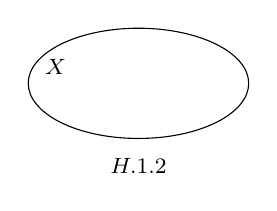
\begin{tikzpicture}[>=stealth,line join=round,line cap=round,font=\footnotesize,scale=.7]
			\draw (1,1) circle (2 and 1);
			\coordinate[label=center:$X$] (X)at(-.5,1.3);
			\coordinate[label=center:$ H.1.2$] (X)at(1,-.5);
	\end{tikzpicture}}
	\immini {$\bullet$ Minh hoạ $T$ là một tập con của $S$ như Hình $1.3$.}
	{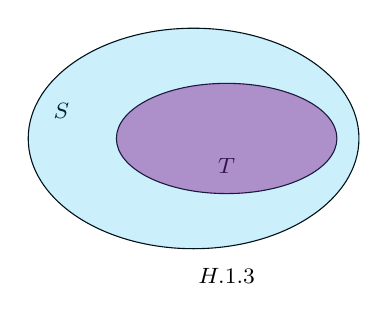
\begin{tikzpicture}[>=stealth,line join=round,line cap=round,font=\footnotesize,scale=.7]
			\coordinate[label=center:$$] (I)at(.4,1);
			\coordinate[label=center:$$] (M)at(1,1);
			\draw (.4,1) circle (3 and 2);
			\coordinate[label=center:$S$] (X)at(-2,1.5);
			\draw (1,1) circle (2 and 1);
			\coordinate[label=center:$T$] (X)at(1,.5);
			\coordinate[label=center:$ H.1.3$] (X)at(1,-1.5);
			\fill[cyan,opacity=.2] (I) ellipse (3 cm and 2 cm)--cycle;
			\fill[violet,opacity=.4] (M) ellipse (2 cm and 1 cm)--cycle;
	\end{tikzpicture}}
\end{tcolorbox}
\subsubsection{Hai tập hợp bằng nhau}
\begin{tcolorbox}
	$S=T \Leftrightarrow \heva{& S \subset T \\ & T \subset S} \Leftrightarrow \forall x,\ (x\in S \Leftrightarrow x \in T)$
\end{tcolorbox}

\subsubsection{Mối quan hệ giữa các tập hợp số}
$\bullet$ Tập hợp các số tự nhiên $\mathbb{N}=\{0 ; 1 ; 2 ; 3 ; \ldots\}$.\\
$\bullet$ Tập hợp các số nguyên $\mathbb{Z}$ gồm các số tự nhiên và các số nguyên âm:
$\mathbb{Z}=\{\ldots ;-2 ;-1 ; 0 ; 1 ; 2 ; \ldots\}$.
$\bullet$ Tập hợp các số hữu tỉ $\mathbb{Q}$ gồm các số viết được dưới dạng phân số $\dfrac{a}{b}$, với $a, b \in \mathbb{Z}, b \neq 0$. Số hữu tỉ còn được biểu diễn dưới dạng số thập phân hữu hạn hoặc vô hạn tuần hoàn.\\
$\bullet$ Tập hợp các số thực $\mathbb{R}$ gồm các số hữu tỉ và các số vô tỉ. Số vô tỉ là các số thập phân vô hạn không tuần hoàn.
\begin{tcolorbox}
	\immini { Mối quan hệ giữa các tập hợp số:  $\mathbb{N} \subset \mathbb{Z} \subset \mathbb{Q} \subset \mathbb{R}$.}
	{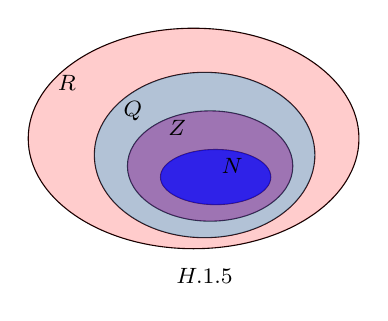
\begin{tikzpicture}[>=stealth,line join=round,line cap=round,font=\footnotesize,scale=.7]
			\path (1.3,1)coordinate[label=center:$$](M) (1.5,.7)coordinate[label=center:$$](N) (1.6,.5)coordinate[label=center:$$](P) (1.7,.3)coordinate[label=center:$$](Q)
			(1.5,-1.5)coordinate[label=center:$H.1.5$](H);
			\draw (1.3,1) circle (3 and 2);
			\draw (1.5,.7) circle (2 and 1.5);
			\draw (1.6,.5) circle (1.5 and 1);
			\draw (1.7,.3) circle (1 and .5);
			\fill[red,opacity=.2] (M) ellipse (3 cm and 2 cm)--cycle;
			\fill[cyan,opacity=.3] (N) ellipse (2 cm and 1.5 cm)--cycle;
			\fill[violet,opacity=.4] (P) ellipse (1.5 cm and 1 cm)--cycle;
			\fill[blue,opacity=.7] (Q) ellipse (1 cm and .5 cm)--cycle;
			\coordinate[label=center:$\mathbb{R}$] (X)at(-1,2);
			\coordinate[label=center:$\mathbb{Q}$] (Q)at(0.2,1.5);
			\coordinate[label=center:$\mathbb{Z}$] (Z)at(1,1.2);
			\coordinate[label=center:$\mathbb{N}$] (N)at(2,.5);
	\end{tikzpicture}}
\end{tcolorbox}
\subsubsection{Các tập con thường dùng của $\mathbb{R}$}
\begin{tcolorbox}
	Một số tập con thường dùng của tập số thực $\mathbb{R}$.\\
	$\bullet$ Khoảng\\
	\immini {$(a ; b)=\{x \in \mathbb{R} \mid a<x<b\}$} {\begin{tikzpicture}[>=stealth,line join=round,line cap=round,font=\footnotesize,scale=1]
			\draw[->] (0,0)--(6,0);
			\path[pattern=north east lines,pattern color=blue] (0,-3pt)rectangle(2,3pt);
			\path[pattern=north east lines,pattern color=blue] (6,-3pt)rectangle(4,3pt);
			\path 
			(2,-0.1)coordinate[label=below:$a$](a) 
			(4,-0.1)coordinate[label=below:$b$](b)
			(2,0)coordinate[label=center:$($](()
			(4,0)coordinate[label=center:$)$](s);
	\end{tikzpicture}}
	\immini {$(a ;+\infty)=\{x \in \mathbb{R} \mid x>a\}$}
	{\begin{tikzpicture}[>=stealth,line join=round,line cap=round,font=\footnotesize,scale=1]
			\draw[->] (0,0)--(6,0);
			\path[pattern=north east lines,pattern color=blue] (0,-3pt)rectangle(2,3pt);
			%\path[pattern=north east lines,pattern color=blue] (6,-3pt)rectangle(4,3pt);
			\path 
			(2,-0.1)coordinate[label=below:$a$](a) 
			%(4,0)coordinate[label=below:$a$](b)
			(2,0)coordinate[label=center:$($](()
			%(4,0)coordinate[label=center:$)$](s)
			;
	\end{tikzpicture}}
	\immini {$(-\infty ; b)=\left\{x \in \mathbb{R} \mid x<b\right\}$}
	{\begin{tikzpicture}[>=stealth,line join=round,line cap=round,font=\footnotesize,scale=1]
			\draw[->] (0,0)--(6,0);
			%\path[pattern=north east lines,pattern color=blue] (0,-3pt)rectangle(2,3pt);
			\path[pattern=north east lines,pattern color=blue] (6,-3pt)rectangle(4,3pt);
			\path 
			%(2,0)coordinate[label=below:$a$](a) 
			(4,-0.1)coordinate[label=below:$b$](b)
			%(2,0)coordinate[label=center:$($](()
			(4,0)coordinate[label=center:$)$](s)
			;
	\end{tikzpicture}}
	\immini {$(-\infty ;+\infty)$}
	{\begin{tikzpicture}[>=stealth,line join=round,line cap=round,font=\footnotesize,scale=1]
			\draw[->] (0,0)--(6,0);
			%\path[pattern=north east lines,pattern color=blue] (0,-3pt)rectangle(2,3pt);
			%\path[pattern=north east lines,pattern color=blue] (6,-3pt)rectangle(4,3pt);
			\path 
			(3,-0.1)coordinate[label=below:$O$](a) 
			%(4,0)coordinate[label=below:$a$](b)
			(3,0)coordinate[label=center:$|$](()
			%(4,0)coordinate[label=center:$)$](s)
			;
	\end{tikzpicture}}
	$\bullet$ Đoạn\\
	\immini {$[a ; b]=\{x \in \mathbb{R} \mid a \leq x \leq b\}$}
	{\begin{tikzpicture}[>=stealth,line join=round,line cap=round,font=\footnotesize,scale=1]
			\draw[->] (0,0)--(6,0);
			\path[pattern=north east lines,pattern color=blue] (0,-3pt)rectangle(2,3pt);
			\path[pattern=north east lines,pattern color=blue] (6,-3pt)rectangle(4,3pt);
			\path 
			(2,-0.1)coordinate[label=below:$a$](a) 
			(4,-0.1)coordinate[label=below:$b$](b)
			(2,0)coordinate[label=center:$[$]()
			(4,0)coordinate[label=center:$\mathrm{]}$](s);
	\end{tikzpicture}}
	$\bullet$ Nửa khoảng\\
	\immini {$[a ; b)=\{x \in \mathbb{R} \mid a \leq x<b\}$}
	{\begin{tikzpicture}[>=stealth,line join=round,line cap=round,font=\footnotesize,scale=1]
			\draw[->] (0,0)--(6,0);
			\path[pattern=north east lines,pattern color=blue] (0,-3pt)rectangle(2,3pt);
			\path[pattern=north east lines,pattern color=blue] (6,-3pt)rectangle(4,3pt);
			\path 
			(2,-0.1)coordinate[label=below:$a$](a) 
			(4,-0.1)coordinate[label=below:$b$](b)
			(2,0)coordinate[label=center:$[$]()
			(4,0)coordinate[label=center:$\mathrm{)}$](s);
	\end{tikzpicture}}
	\immini {$(a ; b]=\{x \in \mathbb{R} \mid a<x \leq b\}$}
	{\begin{tikzpicture}[>=stealth,line join=round,line cap=round,font=\footnotesize,scale=1]
			\draw[->] (0,0)--(6,0);
			\path[pattern=north east lines,pattern color=blue] (0,-3pt)rectangle(2,3pt);
			\path[pattern=north east lines,pattern color=blue] (6,-3pt)rectangle(4,3pt);
			\path 
			(2,-0.1)coordinate[label=below:$a$](a) 
			(4,-0.1)coordinate[label=below:$b$](b)
			(2,0)coordinate[label=center:$($]()
			(4,0)coordinate[label=center:$\mathrm{]}$](s);
	\end{tikzpicture}}
	\immini {$[a ;+\infty)=\{x \in \mathbb{R} \mid x \geq a\}$}
	{\begin{tikzpicture}[>=stealth,line join=round,line cap=round,font=\footnotesize,scale=1]
			\draw[->] (0,0)--(6,0);
			\path[pattern=north east lines,pattern color=blue] (0,-3pt)rectangle(2,3pt);
			%\path[pattern=north east lines,pattern color=blue] (6,-3pt)rectangle(4,3pt);
			\path 
			(2,-0.1)coordinate[label=below:$a$](a) 
			%(4,0)coordinate[label=below:$a$](b)
			(2,0)coordinate[label=center:$[$](()
			%(4,0)coordinate[label=center:$)$](s)
			;
	\end{tikzpicture}}
	\immini {$(-\infty ; b]=\{x \in \mathbb{R} \mid x \leq b\}$}
	{\begin{tikzpicture}[>=stealth,line join=round,line cap=round,font=\footnotesize,scale=1]
			\draw[->] (0,0)--(6,0);
			%\path[pattern=north east lines,pattern color=blue] (0,-3pt)rectangle(2,3pt);
			\path[pattern=north east lines,pattern color=blue] (6,-3pt)rectangle(4,3pt);
			\path 
			%(2,0)coordinate[label=below:$a$](a) 
			(4,-0.1)coordinate[label=below:$b$](b)
			%(2,0)coordinate[label=center:$($](()
			(4,0)coordinate[label=center:$\mathrm{]}$](s)
			;
	\end{tikzpicture}}
\end{tcolorbox}

\subsubsection{Giao của hai tập hợp}
\begin{tcolorbox}
	\immini{Tập hợp gồm các phần tử thuộc cả hai tập hợp $S$ và $T$ gọi là giao của hai tập hợp $S$ và $T$, kí hiệu là $S \cap T$.\\
		$S \cap T=\{x \mid x \in S$ và $x \in T\}$.}
	{\begin{tikzpicture}[>=stealth,line join=round,line cap=round,font=\footnotesize,scale=1]
			\begin{scope}
				\clip (0.5,0) ellipse (1.5 and 1 );
				\fill[pattern = north east lines]	(2.5,0) ellipse (2 and 1.5 );
			\end{scope}
			\draw (0.5,0) ellipse (1.5 and 1 );
			\draw (2.5,0) ellipse (2 and 1.5 );
			\coordinate[label=center:$S\cap T$] (M)at(1.1,.3);
	\end{tikzpicture}}
\end{tcolorbox}
\subsubsection{Hợp của hai tập hợp}
\begin{tcolorbox}
	\immini {Tập hợp gồm các phần tử thuộc tập hợp $S$ hoặc thuộc tập hợp $T$ gọi là hợp của hai tập hợp $S$ và $T$. Kí hiệu là $S \cup T$.
		\[S \cup T=\{x \mid x \in S \text { hoặc } x \in T\}.\]}
	{\begin{tikzpicture}[>=stealth,line join=round,line cap=round,font=\footnotesize,scale=.7]
			\coordinate[label=center:$$] (I)at(0,1);
			\coordinate[label=center:$$] (M)at(1,1);
			\draw[fill,pattern = north east lines] (0,1) circle (1.5 and 1);
			\draw[fill,pattern = north east lines] (1,1) circle (1.5 and 1);
			\coordinate[label=center:$S\cup T$] (X)at(.6,-.5);
			\coordinate[label=center:$S$] (X)at(-1,1);
			\coordinate[label=center:$T$] (X)at(2,1);
	\end{tikzpicture}}
\end{tcolorbox}
\subsubsection{Hiệu của hai tập hợp}
\begin{tcolorbox}
	\immini {$\bullet$ Hiệu của hai tập hợp $S$ và $T$ là tập hợp gồm các phần tử thuộc S nhưng không thuộc $T$, kí hiệu là $S \backslash T$.
		\[S \backslash T=\{x \mid x \in S \text{ và } x \notin T\}\].}
	{\begin{tikzpicture}[>=stealth,line join=round,line cap=round,font=\footnotesize,scale=.8]
			\draw (0.5,0) ellipse (1.5 and 1 );
			\draw (2.5,0) ellipse (1.5 and 1 );
			\fill[pattern = north east lines] (0.5,0) ellipse (1.5 and 1 );
			\fill[fill=white] (2.5,0) ellipse (1.5 and 1 );
			\path 
			(0,.5)coordinate[label=center:$S$](S) (2,.5)coordinate[label=center:$T$](T)
			(1.7,1.5)coordinate[label=center:$S\backslash T$](T) ;
			
	\end{tikzpicture}}
	\immini {$\bullet$ Nếu $T \subset S$ thì $S \backslash T$ được gọi là phần bù của $T$ trong $S$, kí hiệu là $C_{s} T$.}
	{	\begin{tikzpicture}[>=stealth,line join=round,line cap=round,font=\footnotesize,scale=.8]
			\draw (0.5,0) ellipse (1.5 and 1 );
			\draw (.8,0) ellipse (1 and .5 );
			\fill[pattern = north east lines] (0.5,0) ellipse (1.5 and 1 );
			\fill[fill=white] (.8,0) ellipse (1 and .5 );
			\path 
			(-.3,.5)coordinate[label=center:$S$](S) (1,0)coordinate[label=center:$T$](T)
			(1,1.3)coordinate[label=center:$C_S T$](T) ;
			
	\end{tikzpicture}}
\end{tcolorbox}
\subsection{CÁC DẠNG BÀI TẬP}
\begin{dang}{Xác định tập hợp}
	Được mô tả theo 2 cách:
	\begin{enumEX}{1}
		\item  Liệt kê tất cả các phần tử của tập hợp.
		\item  Nêu tính chất đặc trưng.
	\end{enumEX}
\end{dang}
\subsubsection{Ví dụ minh hoạ}
\begin{vd}%[BG10-2022]%[Đỗ Văn Dự]%[0D1Y2-1]
	Cho $D=\{n \in \mathbb{N} \mid n$ là số nguyên tố, $5<n<20\}$.
	\begin{enumEX}{1}
		\item Dùng kí hiệu $\in, \notin$ để viết câu trả lời cho câu hỏi sau: Trong các số $5$; $12$; $17$; $18$, số nào thuộc tập $D$, số nào không thuộc tập $D$?
		\item Viết tập hợp $D$ bằng cách liệt kê các phần tử. Tập hợp $D$ có bao nhiêu phần tử?
	\end{enumEX}
	\loigiai{
		\begin{enumEX}{1}
			\item $5 \notin D$; $12 \notin D$; $17 \in D$; $18 \notin D$.
			\item $D=\{7 ; 11 ; 13 ; 17 ; 19\}$. Tập hợp $D$ có $5$ phần tử.
		\end{enumEX}	
	}
\end{vd}

\begin{vd}%[BG10-2022]%[Đỗ Văn Dự]%[0D1B2-1] 
	Viết mỗi tập hợp sau bằng cách liệt kê các phần tử.
	\begin{enumEX}{2}
		\item $A=\left\{\left. x\in \mathbb{R}\right|\left(2x-x^2\right)\left(3x-2\right)=0\right\}$.
		\item $B=\left\{\left. x\in \mathbb{Z}\right|2x^3-3x^2-5x=0\right\}$.
		\item $C=\left\{\left. x\in \mathbb{Z}\right|2x^2-75x-77=0\right\}$.
		\item $D=\left\{\left. x\in \mathbb{R}\right|(x^2-x-2)(x^2-9)=0\right\}$.
	\end{enumEX}
	\loigiai{
		\begin{enumEX}{1}
			\item Ta giải phương trình\\
			 $\left(2x-x^2\right)\left(2x^2-3x-2\right)=0\Leftrightarrow \hoac{
				& 2x-x^2=0 \\ 
				& 2x^2-3x-2=0}\Leftrightarrow \hoac{
				& x=0\vee x=2 \\ 
				& x=-\dfrac{1}{2}\vee x=2}$.\\
			Do $x\in \mathbb{R}$ nên $A=\left\{-\dfrac{1}{2};0;2\right\}$.
			\item Ta giải phương trình $2x^3-3x^2-5x=0\Leftrightarrow x\left(2x^2-3x-5\right)=0\Leftrightarrow \hoac{&x=0\\&x=-1\\&x=\dfrac{5}{3}}$.\\
			Do $x\in \mathbb{Z}$ nên $B=\left\{0;-1\right\}$.
			\item Ta giải phương trình $2x^2-75x-77=0\Leftrightarrow \hoac{&x=-1\\&x=\dfrac{77}{2}}$.\\
			Do $x\in \mathbb{Z}$ nên $C=\left\{-1\right\}$.
	\end{enumEX}}
\end{vd}

\begin{vd}%[BG10-2022]%[Đỗ Văn Dự]%[0D1B2-1] 
	Viết mỗi tập hợp sau bằng cách liệt kê các phần tử.
	\begin{enumEX}{1}
		\item $A=\left\{\left. n\in {\mathbb{N}}^{*}\right|3<n^2<30\right\}$.
		\item $B=\left\{\left. n\in \mathbb{Z}\right|\left| n\right|<3\right\}$.
		\item $C=\left\{\left. x\right|x=3k\right.$ với $k\in \mathbb{Z}$ và $\left.-4<x<12\right\}$.
		\item $D=\left\{\left. n^2+3\right|n \in \mathbb{N} \text{ và } n<5\right\}$.
	\end{enumEX}
	\loigiai{
		\begin{enumEX}{1}
			\item Với $3<n^2<30$ và $n\in {\mathbb{N}}^{*}$ nên chọn $n=2;3;4;5$.\\
			Vậy $A=\left\{2;3;4;5\right\}$.
			\item  Vì $x<\left| 3\right|\Leftrightarrow-3<x<3$.\\
			Do $x\in \mathbb{Z}$ nên $B=\left\{-2;-1;0;1;2\right\}$.
			\item Ta có $-4<x<12\Leftrightarrow-4<3k<12\Leftrightarrow-\dfrac{4}{3}<k<4$.\\
			Do $k\in \mathbb{Z}$ nên ta chọn $k=\left\{-10;1;2;3\right\}$ suy ra $x=3k=\left\{-3;0;3;6;9\right\}$.\\
			Vậy $C=\left\{-3;0;3;6;9\right\}$.
			\item Vì $n \in \mathbb{N} \text{ và } n<5$ nên chọn  $n=0,1,2;3;4$.\\
			Vậy $A=\left\{3;4;12;19\right\}$.
		\end{enumEX}
	}
\end{vd}

\begin{vd}%[BG10-2022]%[Đỗ Văn Dự]%[0D1K2-1]
	Viết mỗi tập hợp sau bằng cách nêu tính chất đặc trưng.
	\begin{enumEX}{2}
		\item $A=\left\{\dfrac{2}{3};\dfrac{3}{8};\dfrac{4}{15};\dfrac{5}{24};\dfrac{6}{35}\right\}$.
		\item $B=\left\{0;3;8;15;24;35\right\}$.
		\item $C=\left\{-4;1;6;11;16\right\}$.
		\item $D=\left\{1;-2;7\right\}$.
	\end{enumEX}
	\loigiai{
		\begin{enumEX}{2}
			\item $A=\left\{\left. \dfrac{n}{n^2-1}\right|n\in \mathbb{N},2\le n\le 6\right\}$.
			\item $B=\left\{\left. n^2-1\right|n\in \mathbb{N},1\le n\le 6\right\}$.
			\item $C=\left\{\left. n\in \mathbb{N}\right|\right.\left. 5n-4\right\}$.
			\item $D=\left\{\left. x\in \mathbb{R}\right|\left(x-1\right)\left(x+2\right)\left(x-7\right)=0\right\}$.
		\end{enumEX}
	}
\end{vd}
\subsubsection{Bài tập tự luận}
\begin{bt}%[Huỳnh Quy]%[0D1B2-1]
	Liệt kê các phần tử của các tập hợp sau:
	\begin{enumerate}
		\item $A=\left\lbrace n\in \mathbb{N} \mid n<5\right\rbrace$.
		\item $B$ là tập hợp các số tự nhiên lớn hơn $0$ và nhỏ hơn $5$.
		\item $C=\left\lbrace x\in \mathbb{R}\mid (x-1)(x+2)=0\right\rbrace$.
	\end{enumerate}
	\loigiai{
		\begin{enumerate}
			\item $A=\left\lbrace 0;1;2;3;4\right\rbrace$.
			\item $B=\left\lbrace 1;2;3;4\right\rbrace$.
			\item Ta có $(x-1)(x+2)=0 \Leftrightarrow \hoac{&x=1\\&x=-2.}$\\
			Mà $x\in \mathbb{R}$ nên
			$C=\left\lbrace -2;1\right\rbrace$.
		\end{enumerate}
	}
\end{bt}
\begin{bt}%[Huỳnh Quy]%[0D1B2-1]
	Viết các tập hợp sau bằng phương pháp liệt kê:
	\begin{enumerate}
		\item $A=\left\lbrace  x\in \mathbb{Q}\mid (x^2-2x+1)(x^2-5)\right\rbrace=0$.
		\item $B=\left\lbrace x \in \mathbb{N}\mid 5<x^2<40\right\rbrace$.
		\item $C=\left\lbrace x\in \mathbb{Z}\mid x^2<9\right\rbrace$.
		\item $D=\left\lbrace x\in \mathbb{R}\mid \left|2x+1\right|=5\right\rbrace$.
	\end{enumerate}
	\loigiai{
		\begin{enumerate}
			\item Ta có $x\in A\Leftrightarrow\hoac{&x^2-2x+1=0\\&x^2-5=0}\Leftrightarrow\hoac{&x=1\in\mathbb{Q}\\&x=\pm\sqrt{5}\not\in \mathbb{Q}.}$\\
			Vậy $A=\left\lbrace 1\right\rbrace$.
			\item $B=\left\lbrace 3;4;5;6\right\rbrace$.
			\item $C=\left\lbrace -2;-1;0;1;2\right\rbrace$.
			\item Ta có $\left|2x+1\right|=5\Leftrightarrow \hoac{& 2x+1=5 \\ & 2x+1 =-5} \Leftrightarrow \hoac{&x=2\\&x=-3.}$\\
			Vậy $D=\left\lbrace 2;-3\right\rbrace$.
		\end{enumerate}
	}
\end{bt}
\begin{bt}%[Huỳnh Quy]%[0D1B2-1]
	Viết các tập hợp sau bằng cách chỉ ra tính chất đặc trưng cho các phần tử của tập hợp đó.
	\begin{enumerate}
		\item $A=\left\lbrace 0;4;8;12;16;\ldots ;52\right\rbrace$.
		\item $B=\left\lbrace 3;6;9;12;15;\ldots ;51\right\rbrace$.
		\item $C=\left\lbrace 2;5;8;11;14;\ldots ;62\right\rbrace$.
	\end{enumerate}
	\loigiai{
		\begin{enumerate}
			\item $A=\left\lbrace x\in \mathbb{N}\mid 0\le x\le 52 \text{ và } x\;\vdots \;4\right\rbrace$.
			\item $B=\left\lbrace x\in \mathbb{N}\mid 3\le x\le 51 \text{ và } x\;\vdots \;3\right\rbrace$.
			\item $C=\left\lbrace  x\in \mathbb{N}\mid 2\le x\le 62 \text{ và } (x-2)\;\vdots \;3\right\rbrace$.
		\end{enumerate}
	}
\end{bt}
\begin{bt}%[Huỳnh Quy]%[0D1K2-1]
	Viết các tập hợp sau bằng cách chỉ ra tính chất đặc trưng cho các phần tử của tập hợp đó.
	\begin{enumerate}
		\item $A=\left\lbrace 2;3;5;7;11;13;17\right\rbrace$.
		\item $B=\left\lbrace -2;4;-8;16;-32;64\right\rbrace$.
	\end{enumerate}
	\loigiai{
		\begin{enumerate}
			\item $A=\left\lbrace x\in \mathbb{N}\mid x\le 17 \text{ và }x \text{ là số nguyên tố} \right\rbrace$.
			\item $B=\left\lbrace x=(-2)^n\mid n\in \mathbb{N}, 1\le n\le 6 \right\rbrace$.
		\end{enumerate}
	}
\end{bt}

\begin{bt}%[Huỳnh Quy]%[0D1B2-1]
	Tìm một tính chất đặc trưng xác định các phần tử của mỗi tập hợp sau
	\begin{align*}
		A&=\{1; 2; 3; 4; 5; 6; 7; 8; 9\} \\
		B&=\{0; 7; 14; 21; 28\}
	\end{align*}
	\loigiai{
		\begin{align*}
			A&=\{x\in \mathbb{N^*} \mid x\leq 9\} \\
			B&=\{x\in \mathbb{N} \mid x \;\vdots \;7 \text{ và } x\leq 28\}
		\end{align*}
	}
\end{bt}

\begin{dang}{Tập hợp con, xác định tập hợp con}
	Cho tập hợp $A$ gồm $n$ phần tử.
	\begin{enumEX}{1}
		\item  Khi liệt kê tất cả các tập con của $A$, ta liệt kê đầy đủ theo thứ tự:\\		
		\centerline{ $\varnothing$; tập $1$ phần tử; tập $2$ phần tử; tập $3$ phần tử;...; $A$.}
		\item  Số tập con của $A$ là $2^n$.
		\item  Số tập con gồm $k$ phần tử của $A$ là $\mathrm{C}_n^k$.
	\end{enumEX}
\end{dang}
\subsubsection{Ví dụ minh hoạ}
\begin{vd}%[BG10-2022]%[Đỗ Văn Dự]%[0D1Y2-2]
	Cho tập hợp $S=\{2 ; 3 ; 5\}$. Những tập hợp nào sau đây là tập con của $S$?
	$$S_{1}=\{3\};S_{2}=\{0 ; 2\}; S_{3}=\{3 ; 5\}$$.
	\loigiai{
		Các tập hợp $S_{1}=\{3\}$, $S_{3}=\{3 ; 5\}$ là những tập con của $S$.\\
		Tập $S_{2}=\{0 ; 2\}$ không là tập con của $S$.
	}
\end{vd}

\begin{vd}%[BG10-2022]%[Đỗ Văn Dự]%[0D1B2-2]
	Cho tập hợp $A=\left\{2;3;4\right\}$ và $B=\left\{2;3;4;5;6\right\}$.
	\begin{enumEX}{1}
		\item Xác định tất cả tập con có hai phần tử của $A$.
		\item Xác định tất cả tập con có ít hơn hai phần tử của $A$.
		\item Tập $A$ có tất cả bao nhiêu tập con.
		\item Xác định tất cả các tập $X$ thỏa $A \subset X \subset B$.
	\end{enumEX}
		\loigiai{
	\begin{enumEX}{1}		
		\item 	Các tập hợp $S_1=\{2;3\}$, $S_2=\{2;4\}$, $S_3=\{3;4\}$  là những tập con của $A$.\\
			Tập $S_{2}=\{0 ; 2\}$ không là tập con của $S$.
		\item 	Các tập hợp $\varnothing$, $\{2\}$, $\{3\}$, $\{4\}$  là những tập con ít hơn $2$ phần tử của $A$.\\
		\item 	Tập $A$ có tất cả $8$ tập con.
		\item 	 Tất cả các tập $X$ thỏa $A \subset X \subset B$ là $\{2;3;4\}$, $\{2;3;4,5\}$, $\{2;3;4,5,6\}$.	
	\end{enumEX}
		}	
\end{vd}
\subsubsection{Bài tập tự luận}
\begin{bt}%[Huỳnh Quy]%[0D1B2-2]
	Tìm tất cả các tập con của tập $A=\{a,1,2\}$.
	\loigiai{Tập $A$ có $2^3=8$ tập con.
		\begin{itemize}
			\item 0 phần tử: $ \varnothing $.
			\item 1 phần tử: $\{a\}$, $\{1\}$, $\{2\}$.
			\item 2 phần tử: $\{a, 1\}$, $\{a,2\}$, $\{1,2\}$.
			\item 3 phần tử: $\{a,1,2\}$.
	\end{itemize}}
\end{bt}
\begin{bt}%[Huỳnh Quy]%[0D1B2-2]
	Tìm tất cả các tập con có 2 phần tử của tập $A=\{1,2,3,4,5,6\}$.
	\loigiai{$\{1,2\}$,$\{1,3\}$, $\{1,4\}$, $\{1,5\}$, $\{1,6\}$, $\{2,3\}$, $\{2,4\}$, $\{2,5\}$, $\{2,6\}$, $\{3,4\}$, $\{3,5\}$, $\{3,6\}$, $\{4,5\}$, $\{4,6\}$, $\{5,6\}$.}
\end{bt}
\begin{bt}%[Huỳnh Quy]%[0D1B2-2]
	Xác định tập hợp $X$ biết $\{1,2\} \subset X \subset \{1,2,5\}$.
	\loigiai{Ta có
		\begin{itemize}
			\item  Vì $\{1,2\} \subset X$ nên tập hợp $X$ có chứa các phần tử $1,2$.
			\item  Vì $X \subset \{1,2,5\}$ nên các phần tử của tập hợp $X$ có thể là $1,2,5$.
		\end{itemize}
		Khi đó tập hợp $X$ có thể là $\{1,2\}, \{1,2,5\}$.}
\end{bt}
\begin{bt}%[Huỳnh Quy]%[0D1B2-2]
	Xác định tập hợp $X$ biết $\{a,1\} \subset X \subset \{a,b,1,2\}$.
	\loigiai{Ta có
		\begin{itemize}
			\item  Vì $\{a,1\} \subset X$ nên tập hợp $X$ có chứa 2 phần tử là $a,1$.
			\item  Vì $X \subset \{a,b,1,2\}$ nên các phần tử của tập hợp $X$ có thể là $a,b,1,2$.
		\end{itemize}
		Suy ra, tập hợp $X$ có 2 phần tử, 3 phần tử hoặc 4 phần tử.\\
		Khi đó, tập hợp $X$ có thể là $\{a,1\}, \{a,1,2\}, \{a,b,1\}, \{a,b,2\}, \{a,b,1,2\}$.\\
		\underline{\textbf{Cách khác:}} $X=\{a;1\} \cup X'$ với $X' \subset \{b;2\}$. \\
		Vì có $4$ tập hợp $X'$ nên có $4$ tập hợp $X$ thỏa yêu cầu bài toán.}
\end{bt}
\begin{bt}%[Huỳnh Quy]%[0D1K2-2]
	Cho tập hợp $A=\{1;2;3;4;5;6\}$. Tìm tất cả các tập con có $3$ phần tử của tập hợp $A$ sao cho tổng các phần tử này là một số lẻ.
	\loigiai{
		Để tổng của ba số nguyên là một số lẻ thì trong ba số chỉ có một số lẻ hoặc cả ba số đều lẻ. Nói cách khác tập con này của $A$ phải có một số lẻ hoặc ba số lẻ.\\
		Chỉ có một tập con gồm ba số lẻ của $A$ là $\{1;3;5\}$. Các tập con gồm ba số của $A$ trong đó có một số lẻ là: \\
		$\{1;2;4\}$; $\{1;2;6\}$; $\{1;4;6\}$;$\{3;2;4\}$; $\{3;2;6\}$; $\{3;4;6\}$; $\{5;2;4\}$; $\{5;2;6\}$; $\{5;4;6\}$.\\
		\textit{\underline{Nhận xét:} Tổng các số nguyên là một số lẻ khi số số lẻ là số lẻ.}
	}
\end{bt}
\begin{bt}%[Huỳnh Quy]%[0D1K2-2]
	Cho $A=\{n\in\mathbb{N}\mid n \text{ là ước của }2\}$; $B=\{x\in\mathbb{R}\mid (x^2-1)(x-2)(x-4)=0 \}$. Tìm tất cả các tập hợp $X$ sao cho $A\subset X\subset B$.
	\loigiai{ 
		Liệt kê các phần tử của tập hợp $A$ và $B$ ta được : \\
		$A=\{1;2\}$; $B=\{-1;1;2;4\}$.\\
		Muốn tìm tập $X$ thỏa điều kiện $A\subset X\subset B$ đầu tiên ta lấy $X=A$, sau đó ghép thêm các phần tử thuộc $B$ mà không thuộc $A$. Với cách thực hiện như trên, ta có các tập hợp $X$ thỏa mãn yêu cầu bài toán là: $X=A=\{1;2 \}$, rồi ghép thêm vào một phần tử ta được: $\{-1;1;2 \}$;$\{4;1;2 \}$\\
		Ghép thêm vào $A$ hai trong bốn phần tử còn lại của $B$ ta được : $X=B=\{-1;1;2;4\}$
	}
\end{bt}
\begin{dang}{Các phép toán trên tập hợp}
\end{dang}
\subsubsection{Ví dụ minh hoạ}
\begin{vd}%[BG10-2022]%[Đỗ Văn Dự]%[0D1B2-2]
	Cho hai tập hợp:
	$C=\{n \in \mathbb{N} \mid n$ là bội chung của 2 và $3 ; n<30\}$;
	$D=\{n \in \mathbb{N} \mid n$ là bội của $6 ; n<30\}$.
	Chứng minh rằng $C=D$.
	\loigiai{
		Ta có: $C=\{0 ; 6 ; 12 ; 18 ; 24\}$.\\
		$D=\{0 ; 6 ; 12 ; 18 ; 24\}$.\\
		Vậy $C=D$.
	}
\end{vd}

\begin{vd}%[BG10-2022]%[Đỗ Văn Dự]%[0D1Y4-1]
	Viết các tập hợp sau dưới dạng các khoảng, đoạn, nửa khoảng trong $\mathbb{R}$ rồi biểu diễn trên trục số: $C=\{x \in \mathbb{R} \mid 2 \leq x \leq 7\}$; $D=\{x \in \mathbb{R} \mid x<2\}$.
	\loigiai{
		\immini{$C=[2;7]$}{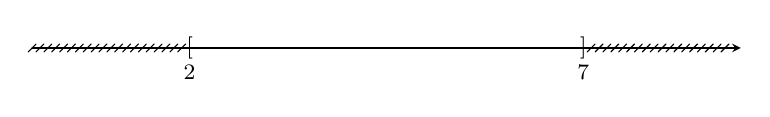
\begin{tikzpicture}[scale=1,>=stealth, font=\footnotesize, line join=round, line cap=round]
				\draw [-stealth] (0,0)--(9,0);
				\path (2,0) node{$[$} (2,-0.1)node[below]{$2$}
				(7,0) node{$]$} (7,-0.1)node[below]{$7$};
				\foreach \x in{0,0.1,...,2} \draw (\x,0)--++(45:.07) (\x,0)--++(-135:.07);
				\foreach \x in{7.1,7.2,...,8.8} \draw (\x,0)--++(45:.07) (\x,0)--++(-135:.07);
		\end{tikzpicture}}
		\immini{$C=(-\infty;2)$}{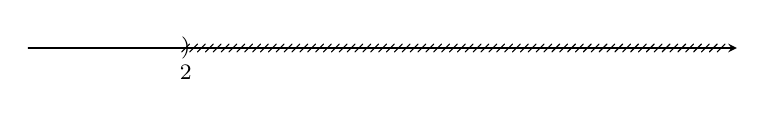
\begin{tikzpicture}[scale=1,>=stealth, font=\footnotesize, line join=round, line cap=round]
				\draw [-stealth] (0,0)--(9,0);
				\path (2,0) node{$)$} (2,-0.1)node[below]{$2$};
				\foreach \x in{2,2.1,...,8.9} \draw (\x,0)--++(45:.07) (\x,0)--++(-135:.07);
		\end{tikzpicture}}	
		
	}
\end{vd}

\begin{vd}%[BG10-2022]%[Đỗ Văn Dự]%[0D1B4-1]
	\begin{enumerate}
		\item Cho hai tập hợp $C=\{4 ; 7 ; 27\}$ và $D=\{2 ; 4 ; 9 ; 27 ; 36\}$. Hãy xác định tập hợp $C \cap D$.
		\item Cho hai tập hợp $E=[1 ;+\infty)$ và $F=(-\infty ; 3]$. Hãy xác định tập hợp $E \cap F$.
	\end{enumerate}
	\loigiai{
		\begin{enumEX}{1}
			\item Giao của hai tập hợp $C$ và $D$ là $C \cap D=\{4 ; 27\}$.
			\item Giao của hai tập hợp $E$ và $F$ là $E \cap F=[1 ; 3]$.\\
			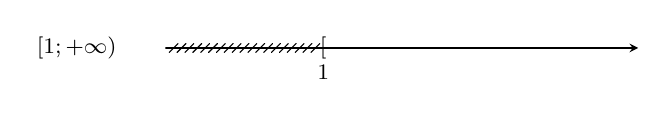
\begin{tikzpicture}[scale=1,>=stealth, font=\footnotesize, line join=round, line cap=round]
				\draw [-stealth] (-1,0)--(5,0);
				\path (1,0) node{$[$} (1,-0.1)node[below]{$1$} (-1.5,0)node[left]{$[1 ;+\infty)$};
				\foreach \x in{-0.9,-0.8,...,0.9} \draw (\x,0)--++(45:.08) (\x,0)--++(-135:.08);
			\end{tikzpicture}\\
			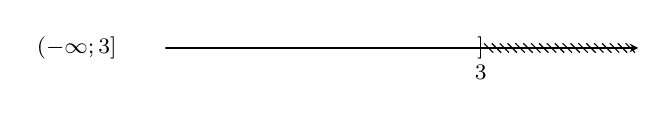
\begin{tikzpicture}[scale=1,>=stealth, font=\footnotesize, line join=round, line cap=round]
				\draw [-stealth] (-1,0)--(5,0);
				\path (3,0) node{$]$} (3,-0.1)node[below]{$3$} (-1.5,0)node[left]{$(-\infty ; 3]$};
				\foreach \x in{3.1,3.2,...,4.9} \draw (\x,0)--++(-45:.08) (\x,0)--++(135:.08);
			\end{tikzpicture}\\
			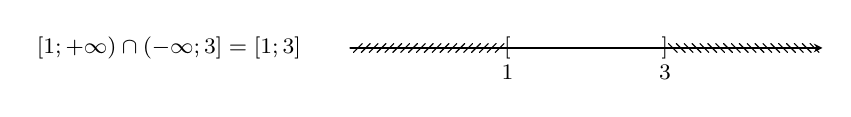
\begin{tikzpicture}[scale=1,>=stealth, font=\footnotesize, line join=round, line cap=round]
				\draw [-stealth] (-1,0)--(5,0);
				\path (3,0) node{$]$} (3,-0.1)node[below]{$3$} 
				(1,0) node{$[$} (1,-0.1)node[below]{$1$} (-1.5,0)node[left]{$[1 ;+\infty)\cap(-\infty ; 3]=[1;3]$}
				;
				\foreach \x in{3.1,3.2,...,4.9} \draw (\x,0)--++(-45:.08) (\x,0)--++(135:.08);
				\foreach \x in{-0.9,-0.8,...,0.9} \draw (\x,0)--++(45:.08) (\x,0)--++(-135:.08);
			\end{tikzpicture}
		\end{enumEX}
	}
\end{vd}
\begin{vd}%[BG10-2022]%[Đỗ Văn Dự]%[0D1B3-1]
	Cho hai tập hợp: $C=\{2 ; 3 ; 4 ; 7\}$; $D=\{-1 ; 2 ; 3 ; 4 ; 6\}$. Hãy xác định tập hợp $C \cup D$.
	\loigiai{
		Hợp của hai tập hợp $C$ và $D$ là $C \cup D=\{-1 ; 2 ; 3 ; 4 ; 6 ; 7\}$.
	}
\end{vd}

\begin{vd}%[BG10-2022]%[Đỗ Văn Dự]%[0D1B3-2]
	Cho các tập hợp: $D=\{-2 ; 3 ; 5 ; 6\}$; $E=\{x \mid x$ là số nguyên tố nhỏ hơn 10$\}$; $X=\{x \mid x$ là số nguyên dương nhỏ hơn 10$\}$.
	\begin{enumEX}{1}
		\item Tìm $D \backslash E$ và $E \backslash D$.
		\item $E$ có là tập con của $X$ không? Hãy tìm phần bù của $E$ trong $X$ (nếu có).
	\end{enumEX}
	\loigiai{
		\begin{enumEX}{1}
			\item Ta có: $E=\{2 ; 3 ; 5 ; 7\}$.\\
			Do đó, $D \backslash E=\{-2 ; 6\}$; $E \backslash D=\{2 ; 7\}$.
			\item Ta có: $X=\{1 ; 2 ; 3 ; 4 ; 5 ; 6 ; 7 ; 8 ; 9\}$. Vậy $E$ là tập con của $X$.\\
			Phần bù của $E$ trong $X$ là $X \backslash E=C_{X} E=\{1 ; 4 ; 6 ; 8 ; 9\}$.
		\end{enumEX}	
	}
\end{vd}

\begin{vd}%[BG10-2022]%[Đỗ Văn Dự]%[0D1B3-1]
	Cho hai tập hợp $A=\left\{0;1;2;3;4\right\}$ và $B=\left\{2;3;4;5;6\right\}$.
	\begin{enumEX}{1}
		\item Tìm các tập hợp $A\cup B, A\cap B, A\backslash B, B\backslash A$.
		\item  Tìm các tập $\left(A\backslash B\right)\cup \left(B\backslash A\right), \left(A\backslash B\right)\cap \left(B\backslash A\right)$.
	\end{enumEX}
	\loigiai{
	\begin{enumEX}{1}
			\item Ta có $A\backslash B=\left\{0;1\right\}$, $B\backslash A=\left\{5;6\right\}$, $A\cup B=\left\{0;1;2;3;4;5;6\right\}$, $A\cap B=\left\{2;3;4\right\}$.
			\item Ta có $\left(A\backslash B\right)\cup \left(B\backslash A\right)=\left\{0;1;5;6\right\}$, $\left(A\backslash B\right)\cap \left(B\backslash A\right)=\varnothing $.
	\end{enumEX}
	}
\end{vd}
\subsubsection{Bài tập tự luận}
\begin{bt}%[Huỳnh Quy]%[0D1B3-2]
	Cho hai tập hợp $A=\{ 1;2;3;4;5\}$ và $B=\{ 0;2;4\}$. Xác định $A\cap B$, $A\cup B$.
	\loigiai{
		Ta có $A\cap B=\{2;4\}$ và $A\cup B=\{0;1;2;3;4;5\}$.
	}
\end{bt}
\begin{bt}%[Huỳnh Quy]%[0D1B3-1]
	Cho hai tập hợp $A=\{1;2;3;5;7\}$ và  $B=\{n\in \mathbb{N} |\, n \text{ là ước số của } 12\}$. Tìm $A\cap B$  và $A\cup B$.
	\loigiai{
		Ta có: $B=\{1;2;3;4;6;12\}$.
		Vậy: $A\cap B=\{ 1;2;3\}$ và $A\cup B=\{ 1;2;3;4;5;6;7;12\}$.
	}
\end{bt}
\begin{bt}%[Huỳnh Quy]%[0D1B3-2]
	Cho hai tập hợp $A$ và $B$. Tìm $A\cap B, A\cup B$ biết
	\begin{enumerate}
		\item $A=\{x\mid x\ \text{là ước nguyên dương của 12} \}$ và 	$B=\{x\mid x\ \text{là ước nguyên dương của 18} \}$.
		\item $A=\{x\mid x\ \text{là ước nguyên dương của 27}\}$ và $B=\{x\mid x\ \text{là ước nguyên dương của 15} \}$.
	\end{enumerate}
	\loigiai{
		\begin{enumerate}
			\item $A=\{1;2;4;6;12\}$, $B=\{1;2;3;6;9;18\}$ $\Rightarrow \begin{cases} A\cap B=\{1;2;6\}\\
				A\cup B=\{1;2;3;4;6;9;12;18\} \end{cases}$
			\item $A=\{1;3;9;27\}$, $B=\{1;3;5;15\}$$\Rightarrow \begin{cases} A\cap B=\{1;3\}\\A\cup B=\{1;3;5;9;15;27\}\end{cases}$
		\end{enumerate}
	}
\end{bt}
\begin{bt}%[Huỳnh Quy]%[0D1B3-1]
	Cho $A$ là tập hợp học sinh lớp $12$ của trường Buôn Ma Thuột và $B$ là tập hợp học sinh của trường Buôn Ma Thuột dự kiến sẽ lựa chọn thi khối $A$ vào các trường đại học. Hãy mô tả các học sinh thuộc tập hợp sau
	\begin{enumEX}{2}
		\item $A\cap B$.
		\item $A\cup B$.
	\end{enumEX}
	\loigiai{
		\begin{enumerate}
			\item $A\cap B$ là tập hợp các học sinh lớp 12 thi khối $A$ của trường Buôn Ma Thuột.
			\item $A\cup B$ là tập hợp các học sinh hoặc lớp 12 hoặc học sinh chọn thi khối A của trường Buôn Ma Thuột. 
		\end{enumerate}
	}
\end{bt}
\begin{bt}%[Huỳnh Quy]%[0D1K3-1]
	Cho tập hợp $B=\{ x\in \mathbb{Z}|\, -4< x \le 4 \}$ và $C=\{ x\in \mathbb{Z}|\, x\le a\}$.
	Tìm số nguyên $a$ để tập hợp $B\cap C=\varnothing $.
	\loigiai{
		Ta có $B=\{-3;-2;-1;0;1;2;3;4\}$, $C=\{\ldots,a-1,a\}$.\\
		Để $B\cap C=\varnothing $ thì  $a\le -4$.
	}
\end{bt}
\begin{bt}%[Huỳnh Quy]%[0D1B3-1]
	Xác định tập hợp $A\cap B$ biết 
	$$A=\{x\in\mathbb{N}|\, x \text { là bội của }3 \}, \,\, B=\{x\in\mathbb{N}|\, x\text { là bội của }7\}.$$
	\loigiai{
		Ta có $A\cap B=\{x\in\mathbb{N}|\, x\text { là bội của }3 \text{ và bội của }7 \}= \{x\in\mathbb{N}|\, x\text {  là bội của  }21\} $.
	}
\end{bt}
\begin{bt}%[Huỳnh Quy]%[0D1B3-2]
	Cho $A$ là tập hợp các số tự nhiên chẵn không lớn hơn $10$, 
	$B=\left\{n\in \mathbb{N}|n\le 6\right\}$ và 
	$C=\left\{n\in \mathbb{N}|4\le n\le 10\right\}$. 
	Hãy tìm $A\cap (B\cup C)$.
	\loigiai{
		Ta có $A=\{0;2;4;6;8;10\}$; $B=\{0;1;2;3;4;5;6\}$ và $C=\{4;5;6;7;8;9;10\}$\\
		$B\cup C=\{0; 1; 2; 3; 4; 5; 6; 7; 8; 9; 10\}$ nên $A\cap (B\cup C)=\{0;2; 4; 6; 8; 10\}$.\\
		\underline{\textbf{Cách khác:}} Vì $B \cup C = \{n \in \mathbb{N} | n \ge 10\}$ nên $A \subset (B \cup C)$.\\
		Do đó $A \cap (B \cup C) = A = \{0;2;4;6;8;10\}$.
	}
\end{bt}
\begin{bt}%[Huỳnh Quy]%[0D1B3-1]
	Cho các tập hợp $A=\{x\in\mathbb{N}\mid x<8\}$ và $B=\{x\in\mathbb{Z}\mid  -3\leq x\leq 5\}$. Tìm $A\cap B$; $A\cup B$.
	\loigiai{
		Ta có $A=\{0;1;2;3;4;5;6;7\}$; $B=\{-3;-2;-1;0;1;2;3;4;5\}$.\\
		Vậy $A\cap B=\{0;1;2;3;4;5\}$ và $A\cup B=\{-3;-2;-1;0;1;2;3;4;5;6;7\}$.
	}
\end{bt}
\begin{bt}%[Huỳnh Quy]%[0D1K3-1]
	Cho các tập hợp $A=\{x \in \mathbb{Z}\big| |x-1|<4\}$, $B=\{x \in \mathbb{Z}\big| |x-1|>2\}$. Tìm $A \cap B$.
	\loigiai{
		Ta có $|x-1|<4 \Leftrightarrow -4<x-1<4 \Leftrightarrow -3<x<5$, $A=\{-2;-1;0;1;2;3;4\}$. \\
		Lại có $|x-1|>2 \Leftrightarrow x<-1\vee x>3$, $B=\{\ldots;-3;-2;4;5;6;\ldots\}$ nên $A \cap B=\{-2;4\}$.
	}
\end{bt}
\begin{bt}%[Huỳnh Quy]%[0D1G3-1]
	Cho các tập hợp $A=\{x\in\mathbb{Z}\,|\, 2m-1<x<2m+3\}$, $B=\{x\in\mathbb{Z}\,\big|\, |x|<2\}$. Tìm $m$ để $A\cap B=\varnothing$.
	\loigiai{
		Ta có $B=\{x\in\mathbb{Z}\,|\, -2<x<2\}=\{-1;0;1\}$ và $A=\{2m,\ldots,2m+2\}$.\\
		$A\cap B=\varnothing \Leftrightarrow \hoac{& 2m+2 \le -2 \\ & 2m \ge 2} \Leftrightarrow \hoac{& m \le -2 \\ & m \ge 1.}$
	}
\end{bt}
\begin{bt}%[Huỳnh Quy]%[0D1B4-1]
	Cho $A=\left[-2;4\right],B=\left(2;+\infty\right),C=(-\infty;3)$. Xác định các tập hợp sau đây và biểu diễn chúng trên trục số.
	\begin{enumerate}
		\item $A\cap B, B\cap C$.
		\item $\mathbb{R}\cap A,\mathbb{R}\cap B$.
	\end{enumerate}
	\loigiai{
		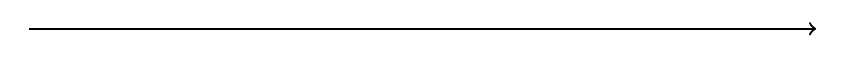
\begin{tikzpicture}[scale=1]
			\draw[->,thick](-4,0) --(6,0);
		\end{tikzpicture}\\
		%
		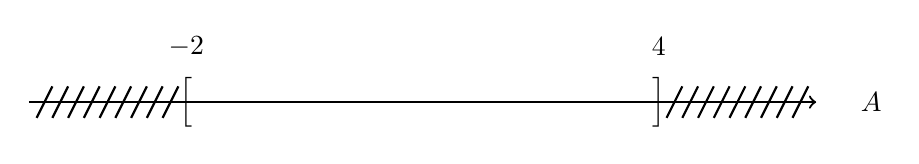
\begin{tikzpicture}[scale=1]
			\draw[->,thick](-4,0) --(6,0) node at (-2,0.7){$-2$} node at (4,0.7){$4$} node at (-2,0) {$\Big [$} node at (4,0) {$\Big ]$}node at (6.7,0){$A$};
			\foreach \b in {-3.8,-3.6,...,-2.2} {\draw[ thick](\b-0.1,-0.2)--(\b+0.1,0.2);}
			\foreach \b in {4.2,4.4,...,5.8} {\draw[ thick](\b-0.1,-0.2)--(\b+0.1,0.2);}
		\end{tikzpicture}\\
		%
		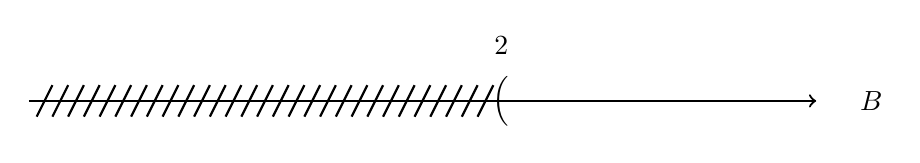
\begin{tikzpicture}[scale=1]
			\draw[->,thick](-4,0) --(6,0) node at (2,0.7){$2$} node at (2,0) {$\Big ($}node at (6.7,0){$B$};
			\foreach \b in {-3.8,-3.6,...,1.8} {\draw[ thick](\b-0.1,-0.2)--(\b+0.1,0.2);}
		\end{tikzpicture}\\
		%
		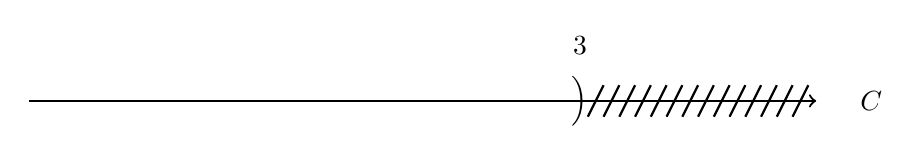
\begin{tikzpicture}[scale=1]
			\draw[->,thick](-4,0) --(6,0) node at (3,0.7){$3$} node at (3,0) {$\Big )$}node at (6.7,0){$C$};
			\foreach \b in {3.2,3.4,...,5.8} {\draw[ thick](\b-0.1,-0.2)--(\b+0.1,0.2);}
		\end{tikzpicture}\\
		%
		\begin{enumerate}
			\item $A\cap B=\left(2;4\right], B\cap C=\left(2;3\right)$.
			\item $\mathbb{R}\cap A=\left[-2;4 \right],\mathbb{R}\cap B=\left(2;+\infty \right)$.
		\end{enumerate}
	}
\end{bt}
\begin{bt}%[Huỳnh Quy]%[0D1B4-2]
	Cho hai tập hợp $A=\lbrace x\in \mathbb{R}\vert  x \leq 2 \rbrace$, $B=\lbrace x\in \mathbb{R}\vert -2< x \rbrace$. Tìm $A\setminus B, B\setminus A$.
	\loigiai{
		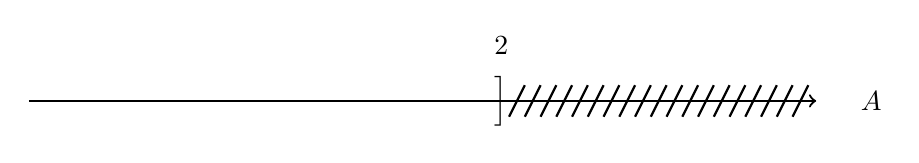
\begin{tikzpicture}[scale=1]
			\draw[->,thick](-4,0) --(6,0) node at (2,0.7){$2$} node at (2,0) {$\Big ]$}node at (6.7,0){$A$};
			\foreach \b in {2.2,2.4,...,5.8} {\draw[ thick](\b-0.1,-0.2)--(\b+0.1,0.2);}
		\end{tikzpicture}\\
		%
		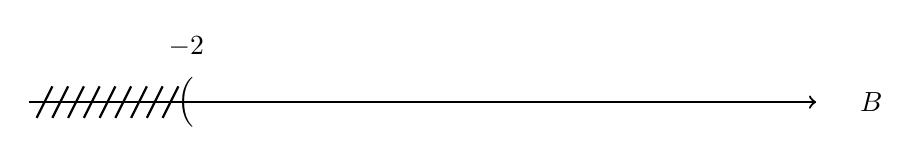
\begin{tikzpicture}[scale=1]
			\draw[->,thick](-4,0) --(6,0) node at (-2,0.7){$-2$} node at (-2,0) {$\Big ($} node at (6.7,0){$B$};
			\foreach \b in {-3.8,-3.6,...,-2.2} {\draw[ thick](\b-0.1,-0.2)--(\b+0.1,0.2);}
		\end{tikzpicture}\\
		$\Rightarrow A\setminus B=\left(-\infty;-2 \right], B\setminus A=\left(2;+\infty \right)$.}
\end{bt}
\begin{bt}%[Huỳnh Quy]%[0D1B4-2] 
	Cho $A=\left[-2;4\right],B=\left(2;+\infty\right),C=(-\infty;3)$. Xác định các tập hợp sau đây và biểu diễn chúng trên trục số.
	\begin{enumerate}
		\item $A\setminus B, B\setminus A$.
		\item $\mathbb{R}\setminus A,\mathbb{R}\setminus B, \mathbb{R}\setminus  C$.
	\end{enumerate}
	\loigiai{
		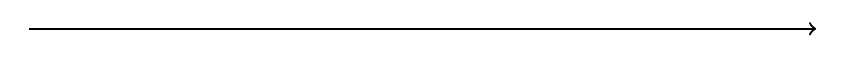
\begin{tikzpicture}[scale=1]
			\draw[->,thick](-4,0) --(6,0);
		\end{tikzpicture}\\
		%
		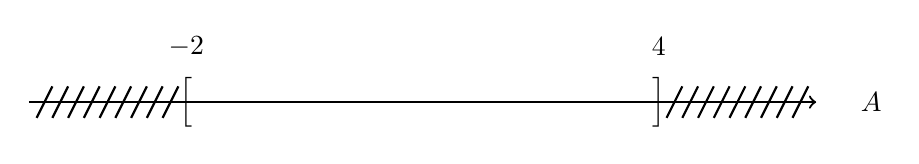
\begin{tikzpicture}[scale=1]
			\draw[->,thick](-4,0) --(6,0) node at (-2,0.7){$-2$} node at (4,0.7){$4$} node at (-2,0) {$\Big [$} node at (4,0) {$\Big ]$}node at (6.7,0){$A$};
			\foreach \b in {-3.8,-3.6,...,-2.2} {\draw[ thick](\b-0.1,-0.2)--(\b+0.1,0.2);}
			\foreach \b in {4.2,4.4,...,5.8} {\draw[ thick](\b-0.1,-0.2)--(\b+0.1,0.2);}
		\end{tikzpicture}\\
		%
		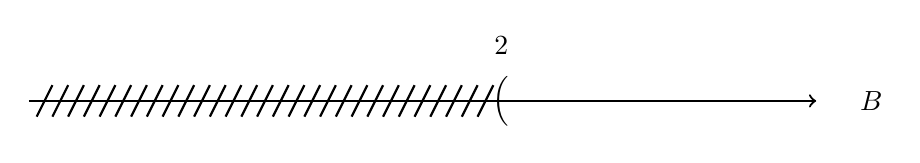
\begin{tikzpicture}[scale=1]
			\draw[->,thick](-4,0) --(6,0) node at (2,0.7){$2$} node at (2,0) {$\Big ($}node at (6.7,0){$B$};
			\foreach \b in {-3.8,-3.6,...,1.8} {\draw[ thick](\b-0.1,-0.2)--(\b+0.1,0.2);}
		\end{tikzpicture}\\
		%
		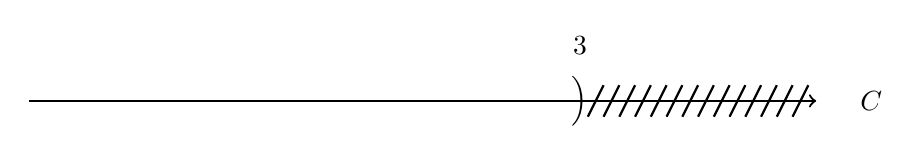
\begin{tikzpicture}[scale=1]
			\draw[->,thick](-4,0) --(6,0) node at (3,0.7){$3$} node at (3,0) {$\Big )$}node at (6.7,0){$C$};
			\foreach \b in {3.2,3.4,...,5.8} {\draw[ thick](\b-0.1,-0.2)--(\b+0.1,0.2);}
		\end{tikzpicture}
		%
		\begin{enumerate}
			\item $A\setminus B=\left[-2;2\right], B\setminus A=\left(4;+\infty\right)$.
			\item $\mathbb{R}\setminus A=\left(\infty;-2\right)\cup\left(4;+\infty \right),\mathbb{R}\setminus B=\left(-\infty;2\right], \mathbb{R}\setminus  C=\left[3;+\infty \right)$.
		\end{enumerate}
	}
\end{bt}
\begin{dang}{Ứng dụng thực tế các phép toán tập hợp}
\end{dang}
\subsubsection{Ví dụ minh hoạ}
\begin{vd}%[BG10-2022]%[Đỗ Văn Dự]%[0D1Y3-3]
	Cho $A$ là tập hợp các học sinh giỏi Toán của trường THPT X và $B$ là tập hợp học sinh giỏi Văn của trường này. Hãy mô tả các học sinh thuộc tập hợp sau\begin{enumEX}{3} 
			\item $A\cup B$.
			\item $A\cap B$.
			\item $A\setminus B$.
			\item $B\setminus A$.
			\item $\left(A\cup B\right)\setminus \left(A\cap B\right)$.
	\end{enumEX}
	\loigiai{
		\immini{
			\begin{enumerate}
				\item $A\cup B$ là tập hợp các học sinh giỏi Toán hoặc giỏi Văn của trường.
				\item $A\cap B$ là tập hợp các học sinh giỏi cả hai môn Toán và Văn của trường.
				\item $A\setminus B$ là tập hợp các học sinh chỉ giỏi Toán, không giỏi Văn.
				\item $B\setminus A$ là tập hợp các học sinh chỉ giỏi Văn, không giỏi Toán.		
				\item $\left(A\cup B\right)\setminus \left(A\cap B\right)$ là tập hợp các học sinh chỉ giỏi Toán hoặc giỏi Văn của trường.	
			\end{enumerate}
		}
		{\begin{tikzpicture}[scale=1, line join=round, line cap=round]	
				\coordinate (A) at (-1.2,0);
				\coordinate (B) at (0.8,0);
				\begin{scope}
					\clip[rotate=20] (A) ellipse (2cm and 1cm); %cat theo elip A
					\fill[rotate=30,pattern=north west lines] (B) ellipse (2cm and 1cm); %to elip B nhung bi cat mat theo phan giao voi elip A
				\end{scope}
				\draw[rotate=20] (A) ellipse (2cm and 1cm) node[fill=white,above]{$A\setminus B$}; %ve lai elip A
				\draw[rotate=30] (B) ellipse (2cm and 1cm) node[fill=white,above,right]{$B\setminus A$}; %ve lai elip B
				\path (-0.2,0.2) node[below]{$A\cap B$};
		\end{tikzpicture}}
	}
\end{vd}
\begin{vd}%[BG10-2022]%[Đỗ Văn Dự]%[0D1B3-3]
	Trong kì thi học sinh giỏi cấp trường, lớp 10C1 có $45$ học sinh trong đó có  $17$ bạn đạt học sinh giỏi Văn, $25$ bạn đạt học sinh giỏi Toán và $13$ bạn học sinh không đạt học sinh giỏi. Tìm số học sinh giỏi cả Văn và Toán của lớp 10C1.
	\loigiai{
		\immini{
			\begin{itemize}			
				\item Gọi $A$, $B$ theo thứ tự là tập hợp các học sinh giỏi Văn và giỏi Toán của lớp. 
				Theo đề ta có $n(A)=17$, $n(B)=25$, $n(A \cup B)= 45-13=32$.
				\item Số học sinh giỏi cả Văn và Toán là $$n(A \cap B )=n(A) + n(B) - n(A \cup B)=25+17-32=10.$$
			\end{itemize}
		}
		{	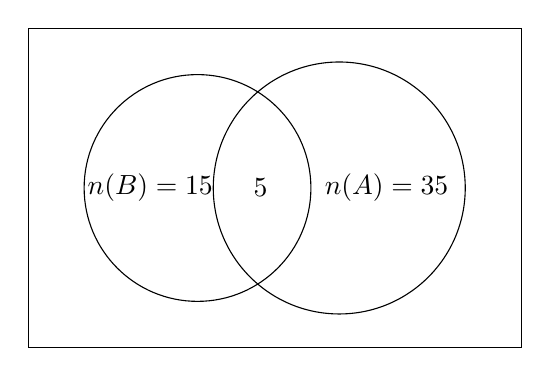
\begin{tikzpicture}[scale=.8]
				\def\radius{2cm}	
				\coordinate (ceni);
				\coordinate[xshift=.9*\radius] (cenii);
				
				\draw (ceni) circle (.9*\radius);
				\draw (cenii) circle (\radius);
				\draw  ([xshift=-25pt,yshift=15pt]current bounding box.north west) 
				rectangle ([xshift=25pt,yshift=-15]current bounding box.south east);
				
				\node[xshift=-.3*\radius] at (ceni) {$n(B)=15$};
				\node[xshift=.3*\radius] at (cenii) {$n(A)=35$};
				\node[xshift=.4*\radius] at (ceni) {$5$};
	\end{tikzpicture}}}
\end{vd}
\begin{vd}%[BG10-2022]%[Đỗ Văn Dự]%[0D1B3-3]
	Một lớp học có $ 50 $ học sinh trong đó có $ 30 $ em biết chơi bóng chuyền, $25$ em biết chơi bóng đá, $ 10 $ em biết chơi cả bóng đá và bóng chuyền. Hỏi có bao nhiêu em không biết chơi môn nào trong hai môn ở trên?
	\loigiai{
		Gọi tập $A$ là tập hợp các học sinh biết chơi bóng chuyền.
		\\Tập $B$ là tập hợp các học sinh biết chơi bóng đá.
		\\Khi đó số học sinh biết chơi ít nhất một trong hai môn bóng chuyền hoặc bóng đá là 
		$$n(A \cup B)=n(A)+n(B)-n(A \cap B)=30+25-10=45.$$
		Vậy số học sinh không biết chơi môn nào là $50-45=5$. 		
	}	
\end{vd}
\begin{vd}%[BG10-2022]%[Đỗ Văn Dự]%[0D1B3-3]
	Trong số $45$ cán bộ được triệu tập để chuẩn bị công tác cho một cuộc hội nghị quốc tế có $25$ cán bộ phiên dịch tiếng Anh, $15$ cán bộ phiên dịch tiếng Pháp, trong đó có $10$ cán bộ vừa phiên dịch được tiếng Anh, vừa phiên dịch được tiếng Pháp. Hỏi
	\begin{enumerate}
		\item Nhóm có bao nhiêu cán bộ được cấp thẻ đỏ, biết rằng muốn được cấp thẻ đỏ cán bộ đó phải phiên dịch được tiếng Anh hoặc phiên dịch được tiếng Pháp.
		\item Nhóm có bao nhiêu cán bộ không phiên dịch được tiếng Anh và không phiên dịch được tiếng Pháp.
	\end{enumerate}
	\loigiai{
		Gọi $A$, $B$ theo thứ tự là tập hợp các cán bộ phiên dịch tiếng Anh và tập hợp các các bộ phiên dịch tiếng Pháp. 
		Theo đề ta có $n(A)=25$, $n(B)=15$, $n(A \cap B)= 10$.
		\begin{enumerate}				
			\item Tập hợp các cán bộ được cấp thẻ đỏ là $A\cup B$.\\
			Vậy số cán bộ được cấp thẻ đỏ là $n(A \cup B)=n(A)+n(B)-n(A \cap B)=25+15-10=30$.
			\item Tập hợp các cán bộ của nhóm không phiên dịch được tiếng Anh và tiếng Pháp chính là số cán bộ không được cấp thẻ đỏ.\\
			Vậy số cán bộ đó là $45-30=15$.
	\end{enumerate}}
\end{vd}
\begin{vd}%[BG10-2022]%[Đỗ Văn Dự]%[0D1B3-3]
	Lớp $10A$ có $15$ bạn thích môn Văn, $20$ bạn thích môn Toán. Trong số các bạn thích văn hoặc toán có $8$ bạn thích cả $2$ môn. Trong lớp vẫn còn $10$ bạn không thích môn nào trong $2$ môn Văn và Toán. Hỏi lớp $10A$ có bao nhiêu học sinh?
	\loigiai{Ta sử dụng sơ đồ Ven.		
		\begin{center}
			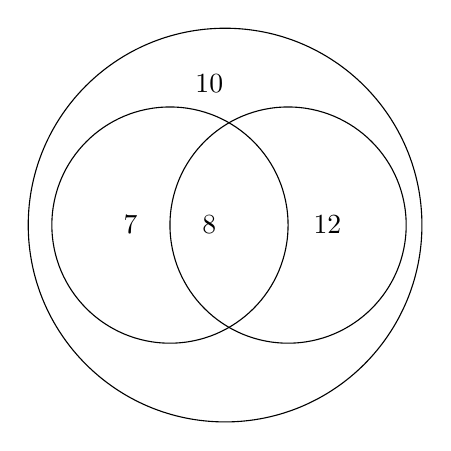
\begin{tikzpicture}
				\draw[] (0.7,0) circle ( 2.5cm);
				\draw[] (0,0) circle ( 1.5cm);
				\draw (1.5,0) circle ( 1.5 cm);
				\draw (-0.5,0) node {$7$};
				\draw (2,0) node {$12$};
				\draw (0.5,0) node {$8$};
				\draw (0.5,1.8) node {$10$};
			\end{tikzpicture}
		\end{center}
		\begin{itemize}
			\item Hình tròn lớn ngoài cùng thể hiện số học sinh cả lớp.\\
			Như vậy, ta có:\\
			\item	Số bạn chỉ thích Văn là $ 15-8=7$(bạn).\\
			\item	Số bạn chỉ thích Toán là $20-8=12$(bạn).\\
			\item	Số học sinh cả lớp là tổng các phần không giao nhau: $7+8+12+10=37$.
		\end{itemize}
	}
\end{vd}

\begin{vd}%[BG10-2022]%[Đỗ Văn Dự]%[0D1B3-3]
	Một lớp có $40$ học sinh, mỗi học sinh đều đăng ký chơi ít nhất $1$ trong $2$ môn thể thao là bóng đá hoặc cầu lông. Có $30$ học sinh có đăng ký môn bóng đá, $25$ học sinh có đăng ký môn cầu lông. Hỏi có bao nhiêu em đăng ký cả $2$ môn.
	\loigiai{
		Gọi $A$ là tập hợp các học sinh đăng kí chơi bóng đá, $B$ là tập học sinh đăng kí chơi cầu lông thì $A\cap B$ là tập hợp các học sinh đăng kí chơi cả hai môn.\\	
		Vậy số học sinh đăng kí chơi cả hai môn là 
		$n(A \cap B)=n(A)+n(B)-n(A \cup B)=30+25-40=15$. }
\end{vd}

\begin{vd}%[BG10-2022]%[Đỗ Văn Dự]%[0D1B3-3]
	Ở xứ sở của thần Thoại ngoài các vị thần thì còn có các sinh vật gồm $27$ con người, $311$ con yêu quái một mắt, $205$ con yêu quái tóc rắn và yêu quái vừa một mắt vừa tóc rắn. Tìm số yêu quái vừa một mắt vừa tóc rắn biết có tổng số sinh vật là 500 con.
	\loigiai{
		\begin{itemize}
			\item Số sinh vật không phải con người là $500-27=473$ (con).
			\item Gọi $A$, $B$ lần lượt là tập hợp yêu quái một mắt và yêu quái tóc rắn. Khi đó $n(A)=311$,  $n(B)=205$, $n(A \cup B)=473$.
			\item Vậy số yêu quái vừa một mắt vừa tóc rắn là $|A \cap B| =311+205-473=43$.
		\end{itemize}
	}
\end{vd}

\begin{vd}%[BG10-2022]%[Đỗ Văn Dự]%[0D1B3-3]
	Mỗi học sinh của lớp $10A$ đều chơi bóng đá hoặc bóng chuyền. Biết rằng có $25$ bạn chơi bóng đá, $20$ bạn chơi bóng chuyền và $10$ bạn chơi cả $2$ môn thể thao. Hỏi lớp $10A$ có bao nhiêu học sinh.
	\loigiai{
		Gọi $A$ là tập hợp các học sinh chơi bóng đá, $B$ là tập các học sinh chơi bóng chuyền. Do đó $A\cap B$ là tập các học sinh chơi cả hai môn.\\
		Theo đề $n(A)=25$, $n(B)=20$, $|A \cap B| =10$.\\
		Vậy số học sinh cả lớp là $|A \cup B| =n(A)+n(B)-n(A \cap B)=25+20-10=35$.}
\end{vd}

\begin{vd}%[BG10-2022]%[Đỗ Văn Dự]%[0D1B3-3]
	Lớp 10A có $45$ học sinh, có $15$ học sinh giỏi và $20$ học sinh xếp hạnh kiểm tốt, trong đó có $10$ bạn vừa học giỏi vừa xếp hạnh kiểm tốt. Các học sinh được học sinh giỏi hoặc hạnh kiểm tốt đều được khen thưởng. Số học sinh được khen thưởng của lớp 10A là là bao nhiêu?
	\loigiai{
		Gọi $A$ là tập hợp các học sinh giỏi, 
		$B$ là tập hợp các học sinh xếp hạnh kiểm tốt.\\
		Khi đó số học sinh được khen thưởng là $n(A \cup B)$.\\
		Vậy số học sinh được khen thưởng là 
		$n(A \cup B)=n(A)+n(B)-n(A \cap B)=15+20-10=25.$		
	}
\end{vd}

\begin{vd}%BT6%[Nguyễn Thành Tuấn]%[0D1K3-3]
	Kết quả thi học kì một của một trường THPT có $48$ thí sinh giỏi môn Toán, $37$ thí sinh giỏi môn Vật Lí,$42$ thí sinh giỏi môn Văn. Biết rằng có $75$ thí sinh giỏi môn Toán hoặc môn Vật lí, $76$ thí sinh giỏi  môn Toán hoặc môn Văn, $66$ thí sinh giỏi môn Vật lí hoặc môn Văn và có $4$ thí sinh giỏi cả ba môn. Hỏi 
	\begin{enumerate}
		\item có bao nhiêu học sinh chỉ giỏi 1 môn.
		\item có bao nhiêu học sinh chỉ giỏi 2 môn.
		\item có bao nhiêu học sinh giỏi ít nhất 1 môn.
	\end{enumerate}
	\loigiai{		
		Gọi $A$, $B$, $C$ theo thứ tự là tập hợp các học sinh giỏi Toán, giỏi Lí và giỏi Văn. Theo đề ta có
		\begin{itemize}
			\item Số học sinh giỏi Toán và Lí là $$n(A \cap B)=n(A)+n(B)-n(A \cup B)=48+37-75=10.$$	
			\item Số học sinh giỏi Toán và Văn là $$n(A \cap C)=n(A)+n(C)-n(A\cup C)=48+42 - 76 = 14 .$$	
			\item Số học sinh giỏi Lí và Văn là $$n(B \cap C)=n(B)+n(C)-n(B\cup C)= 42+37-66=13 .$$	
			\item Số học sinh chỉ giỏi môn Toán $48-10-14+4=28 $.	
			\item Số học sinh chỉ giỏi môn Lí $37-10-13+4=18 $.	
			\item Số học sinh chỉ giỏi môn Văn $42-13-14+4=19 $.
		\end{itemize}
		\begin{center}
			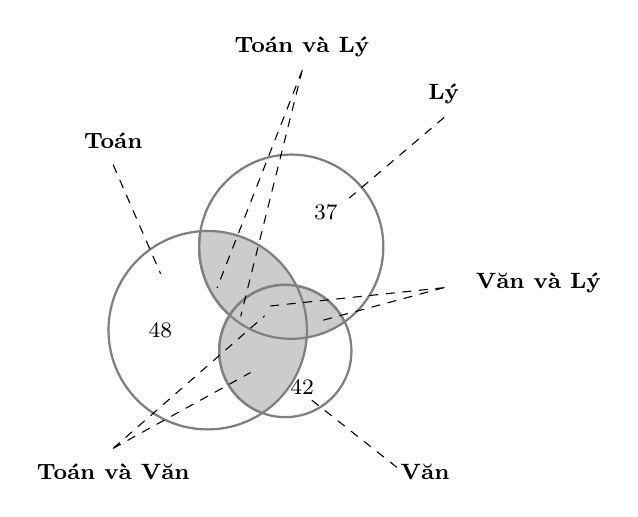
\begin{tikzpicture}[scale=0.6,>=stealth, font=\footnotesize, line join=round, line cap=round]	
				\def\firstcircle{(0,0) circle (2.1cm)}
				\def\secondcircle{(45:2.5cm) circle (1.95cm)}
				\def\thirdcircle{(-15:1.7cm) circle (1.4cm)}
				\colorlet{circle edge}{black!50}
				\colorlet{circle area}{black!20}
				\tikzset{filled/.style={fill=circle area, draw=circle edge, thick},
					outline/.style={draw=circle edge, thick}}
				\draw \firstcircle;
				\draw \secondcircle;
				\draw \thirdcircle;
				\begin{scope}
					\clip \firstcircle;
					\fill[filled] \secondcircle;
				\end{scope}
				\begin{scope}
					\clip \firstcircle;
					\fill[filled] \thirdcircle;
				\end{scope}
				\begin{scope}
					\clip \secondcircle;
					\fill[filled] \thirdcircle;
				\end{scope}  
				\node at (-1,0){48};  
				%\node at (0.5,1){3}; 
				%	\node at (1.2,0.3){1};  
				%	\node at (2.3,0.3){1};      
				%	\node at (1,-0.5){2};   
				\node at (2,-1.2){42};     
				\node at (2.5,2.5){37}; 
				\draw[outline] \firstcircle
				\secondcircle  \thirdcircle;    
				\node at (-2,4) {\textbf{Toán}};
				\node at (2,6) {\textbf{Toán và Lý}};
				\node at (5,5) {\textbf{Lý}};
				\node at (7,1) {\textbf{Văn và Lý}};   
				\node at (4.6,-3) {\textbf{Văn}};
				\node at (-2,-3) {\textbf{Toán và Văn}};
				\draw[dashed] (-2,3.5) -- (-1,1.2) 
				(2,5.5) -- (0.7,0.3) 
				(2,5.5) -- (0.2,0.9)
				(5,4.5) -- (3,2.8)
				(5,0.9) -- (1.2,0.5)
				(5,0.9) -- (2.4,0.2)
				(4,-2.9) -- (2.1,-1.4)
				(-2,-2.5) -- (1.2,0.3)
				(-2,-2.5) -- (0.9,-0.9)	;
		\end{tikzpicture}	
		\end{center}
		
		\begin{enumerate}	
			\item Số học sinh chỉ giỏi đúng 1 môn là $28+18+19=65$. 
			\item Số học sinh chỉ giỏi đúng 2 môn là $10+14+13-4\cdot2=25 $. 
			\item Số học sinh giỏi ít nhất một môn là $65+25+4=94$.
		\end{enumerate}
	}
\end{vd}
\begin{vd}%[BG10-2022]%[Đỗ Văn Dự]%[0D1K3-3]
	Một nhóm học sinh giỏi các bộ môn: Anh, Toán, Văn. Có $18$ em giỏi Văn, $10$ em giỏi Anh, $12$ em giỏi Toán, $3$ em giỏi Văn và Toán, $4$ em giỏi Toán và Anh, $5$ em giỏi Văn và Anh, $2$ em giỏi cả ba môn. Hỏi nhóm đó có bao nhiêu em?
	\loigiai{
		Gọi $A$ là tập hợp những học sinh giỏi Anh,
		$T$ là tập hợp những học sinh giỏi toán,
		$V$ là tập hợp những học sinh giỏi Văn.
		Ta có\\
		$\bullet$ $n\left( V \right)=18,\; n\left( A \right)=10$,\; $n\left( T \right)=12$,\; 
		$n(V\cap T)=3,\;n(T\cap A)=4,\;n(V\cap A)=5$,\; $n(A\cap B\cap C)=2$.\\
		$\bullet$  $\begin{aligned}[t] n(V\cup A\cup T)&=n\left( V \right)+n\left( A \right)+n\left( T \right)-\left[ n(V\cap A)+n(A\cap T)+n(T\cap V) \right]+n\left( V\cap A\cap T \right)\\ &=
		18+10+12-\left[ 3+4+5 \right]+2=30 \end{aligned}$.\\
		Vậy nhóm đó có 30 em.}
\end{vd}

\begin{vd}%[BG10-2022]%[Đỗ Văn Dự]%[0D1K3-3]
	Trong số $42$ học sinh của lớp 10A có $13$ bạn được xếp loại học lực giỏi, $22$ bạn được xếp loại hạnh kiểm tốt, trong đó $7$ bạn vừa học lực giỏi, vừa có hạnh kiểm tốt. Hỏi lớp 10A có bao nhiêu bạn được khen thưởng? Biết rằng muốn được khen thưởng thì bạn đó phải có học lực giỏi hoặc có hạnh kiểm tốt.
	\loigiai{
		Gọi tập hợp các học sinh học lực giỏi là $G$, tập hợp các bạn học sinh hạnh kiểm tốt là $T$. Khi đó tập hợp các bạn học sinh vừa có học lực giỏi là, vừa có hạnh kiểm tốt là $G\cap T$, tập hợp các bạn học sinh đạt học lực giỏi hoặc hạnh kiểm tốt là $G\cup T$. Ta có \\
		$n(G)=13$, $n(T)=22$, $n(G\cap T)=7$.\\
		$n(G\cup T)=n(G)+n(T)-n(G\cap T)=13+22-7=28.$}
\end{vd}

\begin{vd}%[BG10-2022]%[Đỗ Văn Dự]%[0D1K3-3]
	Một nhóm học sinh giỏi các bộ môn: Anh, Toán, Văn. Có $ 18 $ em giỏi Văn, $ 10 $ em giỏi Anh, $ 12 $ em giỏi Toán, $ 3 $ em giỏi Văn và Toán, $ 4 $ em giỏi Toán và Anh, $ 5 $ em giỏi Văn và Anh, $ 2 $ em giỏi cả ba môn. Hỏi nhóm đó có bao nhiêu em?
	\loigiai{
		\begin{center}
			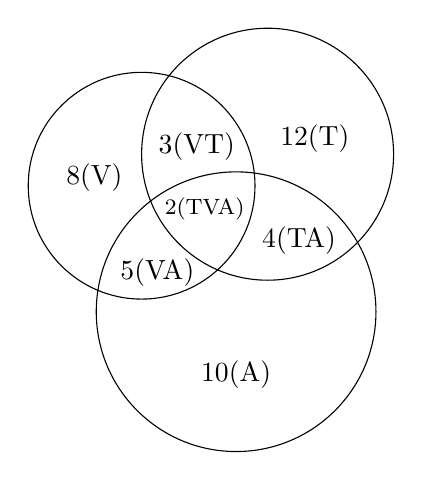
\begin{tikzpicture}[scale=.8]
				\def\radius{2cm}	
				\coordinate (ceni);
				\coordinate[xshift=.8*\radius, yshift=.2*\radius] (cenii);
				\coordinate[xshift=.6*\radius,yshift=-.8*\radius] (ceniii);
				\draw (ceni) circle (.9*\radius);
				\draw (cenii) circle (\radius);
				\draw (ceniii) circle (1.11*\radius);
				
				\node[xshift=-.3*\radius, yshift=.05*\radius] at (ceni) {$8$(V)};
				\node[xshift=.35*\radius, yshift=.25*\radius] at (ceni) {$3$(VT)};
				\node[xshift=.1*\radius, yshift=-.55*\radius] at (ceni) {$5$(VA)};
				\node[xshift=.4*\radius, yshift=-.15*\radius] at (ceni) {{\footnotesize $2$(TVA)}};
				\node[xshift=.2*\radius, yshift=-.55*\radius] at (cenii) {$4$(TA)};
				\node[xshift=1.1*\radius,yshift=.3*\radius] at (ceni) {$12$(T)};
				\node[yshift=-.4*\radius] at (ceniii) {$10$(A)};
			\end{tikzpicture}
		\end{center}
		Ký hiệu $ A $ là tập hợp những học sinh giỏi Anh,\\
		$ T $ là tập hợp những học sinh giỏi Toán,\\
		$ V $ là tập hợp những học sinh giỏi Văn.\\
		$\bullet$ $n(V)=18,\; n(A)=10,\; n(T)=12$,\\
		$\bullet$ $n(T \cap V)=3,\; n(T \cap A)=4,\; n(V \cap A)=5, n(A \cap B \cap C)=2$.\\
		Số học sinh của nhóm là
		\begin{eqnarray*}
			n(V \cup A \cup T)&=&n(V)+n(A)+n(T)-n(V \cap A)-n(T \cap A)-n(T \cap V)+n(A \cap B \cap C)\\
			&=&18+10+12-(3+4+5)+2=30.
		\end{eqnarray*}
		Vậy nhóm đó có $ 30 $ em.
	}
\end{vd}

\begin{vd}%[BG10-2022]%[Đỗ Văn Dự]%[0D1K3-3]
	Có $44$ học sinh giỏi, mỗi em giỏi ít nhất một môn. Có $22$ em giỏi Văn, $25$ em giỏi Toán, $20$ em giỏi Anh. Có $8$ em giỏi đúng hai môn Văn, Toán; Có $7$ em giỏi đúng hai môn Toán, Anh; Có $6$ em giỏi đúng hai môn Anh, Văn. Hỏi có bao nhiêu em giỏi cả ba môn Văn, Toán, Anh?
	\loigiai{
		Ta có \\
		$n\left( V \right)=22,\;n\left( T \right)=25$,\; $n\left( A \right)=20$\\
		$n((V\cap T)\setminus A)=8,\;n((T\cap A)\setminus V)=7,\;n((V\cap A)\setminus T)=6,\; n(V\cup T\cup A)=44$.\\
		$n(V\cup A\cup T)=n\left( V \right)+n\left( A \right)+n\left( T \right)-n(V\cap A)-n(A\cap T)-n(T\cap V)+n\left( V\cap A\cap T \right)$\\
		$  \Leftrightarrow  44=22+20+25-6-7-8+4n\left( V\cap A\cap T \right)$.\\
		$\Rightarrow n\left( V\cap A\cap T \right)=1$.
	}
\end{vd}
\begin{vd}%[BG10-2022]%[Đỗ Văn Dự]%[0D1B3-3]
	Để thành lập đội tuyển học sinh giỏi khối $ 10 $, nhà trường tổ chức thi chọn các môn Toán, Văn, Anh trên tổng số $ 111 $ học sinh. Kết quả có: $ 70 $ học sinh giỏi Toán, $ 65 $ học sinh giỏi Văn, $ 62 $ học sinh giỏi Anh. Trong đó có $ 49 $ học sinh giỏi cả hai môn Văn và Toán, $ 32 $ học sinh giỏi cả hai môn Toán và Anh, $ 34 $ học sinh giỏi cả hai môn Văn và Anh. Xác định số học sinh giỏi cả ba môn Văn, Toán, Anh. Biết rằng có $ 6 $ học sinh không đạt yêu cầu cả ba môn.
	\loigiai{
		\immini
		{Có $ 111-6=105 $ học sinh thi đạt ít nhất $ 1 $ môn.\\
			Gọi $ A $ là số học sinh giỏi môn Toán và Tiếng Anh nhưng không giỏi Văn.\\
			Gọi $ B $ là số học sinh giỏi môn Toán và Văn nhưng không giỏi Tiếng Anh.\\
			Gọi $ C $ là số học sinh giỏi môn Văn và Tiếng Anh nhưng không giỏi Toán.\\
			Gọi $ D $ là số học sinh giỏi cả ba môn. Ta có hệ:\\
			$\begin{cases}
				B+D=49\\
				A+D=32\\
				C+D=34\\
				70+65+62-(A+B+C+2D)=105
			\end{cases}\\
			\Rightarrow 92=32-D+49-D+34-D+2D\\
			\Rightarrow D=23$.\\
			Vậy có $ 23 $ học sinh giỏi cả ba môn.
		}
		{
			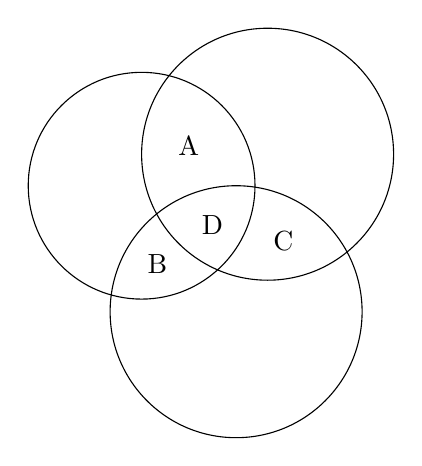
\begin{tikzpicture}[scale=.8]
				\def\radius{2cm}	
				\coordinate (ceni);
				\coordinate[xshift=.8*\radius, yshift=.2*\radius] (cenii);
				\coordinate[xshift=.6*\radius,yshift=-.8*\radius] (ceniii);
				\draw (ceni) circle (.9*\radius);
				\draw (cenii) circle (\radius);
				\draw (ceniii) circle (\radius);
				
				\node[xshift=.3*\radius, yshift=.25*\radius] at (ceni) {A};
				\node[xshift=.1*\radius, yshift=-.5*\radius] at (ceni) {B};
				\node[xshift=.45*\radius, yshift=-.25*\radius] at (ceni) {D};
				\node[xshift=.1*\radius, yshift=-.55*\radius] at (cenii) {C};
		\end{tikzpicture}}
	}
\end{vd}
\subsubsection{Bài tập tự luận}
\begin{bt}%[Huỳnh Quy]%[0D1B3-3]
	Mỗi học sinh của lớp $10A$ đều chơi bóng đá hoặc bóng chuyền. Biết rằng có $25$ bạn chơi bóng đá, $20$ bạn chơi bóng chuyền và $10$ bạn chơi cả $2$ môn thể thao. Hỏi lớp $10A$ có bao nhiêu học sinh.
	\loigiai{
		Ngoài sơ đồ Ven ta có thể dùng công thức số phần tử. Gọi $A$ là tập hợp các học sinh chơi bóng đá, $B$ là tập các học sinh chơi bóng chuyền. Do đó $A\cap B$ là tập các học sinh chơi cả hai môn. Ta có
		$$n(A)=25, n(B)=20, n(A \cap B) =10.$$
		Số học sinh cả lớp là số phần tử của tập $A \cup B$ nên $n(A \cup B) = 25+20-10=35$ (học sinh).
	}
\end{bt}
\begin{bt}%[Huỳnh Quy]%[0D1B3-3]
	Lớp $10{{B}_{1}}$ có $7$ học sinh giỏi Toán, $5$ học sinh giỏi Lý, $6$ học sinh giỏi Hóa, $3$ học sinh giỏi cả Toán và Lý, $4$ học sinh giỏi cả Toán và Hóa, $2$ học sinh giỏi cả Lý và Hóa, $1$ học sinh giỏi cả $3$ môn Toán, Lý, Hóa. Tính số học sinh giỏi ít nhất một môn (Toán, Lý, Hóa) của lớp $10{{B}_{1}}$.
	\loigiai{
		Ta dùng biểu đồ Ven để giải:
		\begin{center}
			\begin{tikzpicture}
				\def\firstcircle{(0,0) circle (1.5cm)}
				\def\secondcircle{(45:2.5cm) circle (2cm)}
				\def\thirdcircle{(-15:1.7cm) circle (1.4cm)}
				\colorlet{circle edge}{black!50}
				\colorlet{circle area}{black!20}
				\tikzset{filled/.style={fill=circle area, draw=circle edge, thick},
					outline/.style={draw=circle edge, thick}}
				\draw \firstcircle;
				\draw \secondcircle;
				\draw \thirdcircle;
				\begin{scope}
					\clip \firstcircle;
					\fill[filled] \secondcircle;
				\end{scope}
				\begin{scope}
					\clip \firstcircle;
					\fill[filled] \thirdcircle;
				\end{scope}
				\begin{scope}
					\clip \secondcircle;
					\fill[filled] \thirdcircle;
				\end{scope}  
				\node at (-1,0){1};  
				\node at (0.5,1){2}; 
				\node at (1,0.3){1};  
				\node at (2,0.3){1};      
				\node at (1,-0.5){3};   
				\node at (2,-1){1};     
				\node at (3,2.5){1}; 
				\draw[outline] \firstcircle
				\secondcircle  \thirdcircle;    
				\node at (-2,4) {\textbf{Toán}};
				\node at (2,6) {\textbf{Giỏi Toán + Lý}};
				\node at (5,5) {\textbf{Lý}};
				\node at (7,1) {\textbf{Giỏi Hóa + Lý}};   
				\node at (5,-3) {\textbf{Hóa}};
				\node at (-2,-3) {\textbf{Giỏi Toán + Hóa}};
				\draw[->] (-2,3.5) -- (-1,1.2) 
				(2,5.5) -- (0.7,0.3) 
				(2,5.5) -- (0.2,0.9)
				(5,4.5) -- (3.6,2.5)
				(5,0.9) -- (1.2,0.5)
				(5,0.9) -- (2.4,0.2)
				(4,-2.9) -- (2,-1.8)
				(-2,-2.5) -- (1.2,0)
				(-2,-2.5) -- (0.9,-0.9)
				;
			\end{tikzpicture}
		\end{center}
		Nhìn vào biểu đồ, số học sinh giỏi ít nhất $1$ trong $3$ môn là: $1+2+1+3+1+1+1=10$}
\end{bt}
\begin{bt}%[Huỳnh Quy]%[0D1B3-3]
	Lớp $10{{\text{A}}_{1}}$ có $7$ học sinh giỏi Toán, $5$ học sinh giỏi Lý, $6$ học sinh giỏi Hóa, $3$ học sinh giỏi cả Toán và Lý, $4$ học sinh giỏi cả Toán và Hóa, $2$ học sinh giỏi cả Lý và Hóa, $1$ học sinh giỏi cả $3$ môn Toán, Lý, Hóa. Tính số học sinh giỏi đúng hai môn học của lớp $10{{\text{A}}_{1}}$.
	\loigiai{
		\begin{center}
			\begin{tikzpicture}
				\def\firstcircle{(0,0) circle (1.5cm)}
				\def\secondcircle{(45:2.5cm) circle (2cm)}
				\def\thirdcircle{(-15:1.7cm) circle (1.4cm)}
				\colorlet{circle edge}{black!50}
				\colorlet{circle area}{black!20}
				\tikzset{filled/.style={fill=circle area, draw=circle edge, thick},
					outline/.style={draw=circle edge, thick}}
				\draw \firstcircle;
				\draw \secondcircle;
				\draw \thirdcircle;
				\begin{scope}
					\clip \firstcircle;
					\fill[filled] \secondcircle;
				\end{scope}
				\begin{scope}
					\clip \firstcircle;
					\fill[filled] \thirdcircle;
				\end{scope}
				\begin{scope}
					\clip \secondcircle;
					\fill[filled] \thirdcircle;
				\end{scope}  
				\node at (-1,0){1};  
				\node at (0.5,1){2}; 
				\node at (1,0.3){1};  
				\node at (2,0.3){1};      
				\node at (1,-0.5){3};   
				\node at (2,-1){1};     
				\node at (3,2.5){1}; 
				\draw[outline] \firstcircle
				\secondcircle  \thirdcircle;    
				\node at (-2,4) {\textbf{Toán}};
				\node at (2,6) {\textbf{Giỏi Toán + Lý}};
				\node at (5,5) {\textbf{Lý}};
				\node at (7,1) {\textbf{Giỏi Hóa + Lý}};   
				\node at (5,-3) {\textbf{Hóa}};
				\node at (-2,-3) {\textbf{Giỏi Toán + Hóa}};
				\draw[->] (-2,3.5) -- (-1,1.2) 
				(2,5.5) -- (0.7,0.3) 
				(2,5.5) -- (0.2,0.9)
				(5,4.5) -- (3.6,2.5)
				(5,0.9) -- (1.2,0.5)
				(5,0.9) -- (2.4,0.2)
				(4,-2.9) -- (2,-1.8)
				(-2,-2.5) -- (1.2,0)
				(-2,-2.5) -- (0.9,-0.9)
				;
			\end{tikzpicture}
		\end{center}
		Dựa vào biểu đồ ven trên, ta có số học sinh giỏi đúng hai môn học là $2+1+3=6$}
\end{bt}

\subsection{Bài tập trắc nghiệm}
\Opensolutionfile{ans}[ans/ans-0D1-2-TN]
\begin{ex}%[Bài giảng Toán 10 - 2022]%[Nhật Thiện]%[0D1Y3-1]
	Cho hai tập hợp $X=\{1;3;5;8\}$, $Y=\{3;5;7;9\}$. Tập hợp $X\cup Y$ bằng tập hợp nào sau đây?
	\choice
	{$\{1;3;5\}$}
	{$\{3;5\}$}
	{$\{1;7;9\}$}
	{\True $\{1;3;5;7;8;9\}$}
	\loigiai{
		Ta có $X\cup Y=\{1;3;5;7;8;9\}$.
	}
\end{ex}
\begin{ex}%[Bài giảng Toán 10 - 2022]%[Nhật Thiện]%[0D1Y3-2]
	Cho hai tập hợp $A=\{1;2;3;4;5\}$ và $B=\{0;2;4;6;8\}$. Tìm $A\setminus B$.
	\choice
	{$A\setminus B=\{2;4\}$}
	{\True $A\setminus B=\{1;3;5\}$}
	{$A\setminus B=\{0;1;3;5\}$}
	{$A\setminus B=\{0;6;8\}$}
	\loigiai{
		Ta có $A\setminus B=\{1;3;5\}$.
	}
\end{ex}
\begin{ex}%[Bài giảng Toán 10 - 2022]%[Nhật Thiện]%[0D1B3-1]
	Cho hai tập hợp $ A=\left\lbrace x\in \mathbb{R}\,\mid\,(2x-x^2)(x-1)=0 \right\rbrace$, $ B=\left\lbrace n \in \mathbb{N}\,\mid\,0<n^2<10 \right\rbrace$. Chọn mệnh đề đúng?
	\choice
	{\True $A \cap B =\left\lbrace 1;2 \right\rbrace $}
	{$A \cap B =\left\lbrace 2 \right\rbrace $}
	{ $A \cap B =\left\lbrace 0;1;2;3 \right\rbrace $}
	{$A \cap B =\left\lbrace 0;3 \right\rbrace $}
	\loigiai{
		Ta có
		\begin{itemize}
			\item $ (2x-x^2)(x-1)=0\Leftrightarrow \hoac{& x=0 \\ &x=1\\&x=2 }\Rightarrow A=\left\lbrace 0;1;2 \right\rbrace  $.
			\item  $ B= \left\lbrace 1;2;3 \right\rbrace$.
		\end{itemize}
		Suy ra $ A\cap B= \left\lbrace 1;2 \right\rbrace$.}
\end{ex}
\begin{ex}%[Bài giảng Toán 10 - 2022]%[Nhật Thiện]%[0D1B3-1]
	Cho các tập hợp $A=\left\{ x\in \mathbb{N} \ | \ (4-x^2)(x^2-5x+4)=0 \right\}; B = \left\{ x\in \mathbb{Z} \ | \ x \text{ là ước của } 4 \right\}$. Tập hợp $A \cap B$ là
	\choice
	{$\{-2,1,2,4\}$}
	{\True $\{1,2,4\}$}
	{$\{2,4\}$}
	{$\{-4,-2,-1,1,2,4\}$}
	\loigiai{
		Ta có $(4-x^2)(x^2-5x+4)=0 \Leftrightarrow \hoac{&4-x^2=0\\&x^2-5x+4=0} \Leftrightarrow \hoac{&x=2\\&x=-2\\&x=1\\&x=4.}$\\
		Vì $x\in \mathbb{N}$ nên $x \in \{1,2,4\}$.\\
		Do đó $A=\{1,2,4\} \quad (1)$.\\
		Ta có các ước của $4$ là $\pm 1, \pm 2, \pm 4$.\\
		Do đó $B=\{-4,-2,-1,1,2,4\} \quad (2)$.\\
		Từ $(1), (2)$ ta có $A \cap B = \{1,2,4\}$.
	}
\end{ex}
\begin{ex}%[Bài giảng Toán 10 - 2022]%[Nhật Thiện]%[0D1Y4-2]
	Cho hai tập hợp $A = \left(-5;7\right)$ và $B = \left(1;+\infty\right)$. Tìm $A\setminus B$.
	\choice
	{\True $A\setminus B = \left(-5;1\right]$}
	{$A\setminus B = \left(-5;1\right)$}
	{$A\setminus B = \left[7;+\infty\right)$}
	{$A\setminus B = \left(7;+\infty\right)$}
	\loigiai{
		Ta có $A\setminus B = \left(-5;1\right]$.
	}
\end{ex}
\begin{ex}%[Bài giảng Toán 10 - 2022]%[Nhật Thiện]%[0D1Y4-2]
	Cho hai tập hợp $A=\left[ -2;4\right)$ và $B=\left(0;+\infty\right)$. Tìm khẳng định đúng.
	\choice
	{$A\cup B=\left(4;+\infty\right)$}
	{\True $A\cap B=\left(0;4\right)$}
	{$B\setminus A=\left[ -2;+\infty\right)$}
	{$A\setminus B=\left[ -2;0\right)$}
	\loigiai{
		$A\cup B=[-2;+\infty) \rightarrow $ loại.\\
		$A\cap B = (0;4) \rightarrow$ chọn.\\
		$B\setminus A = [4;+\infty) \rightarrow$ loại.\\
		$A\setminus B = [-2;0] \rightarrow$ loại.
	}
\end{ex}
\begin{ex}%[Bài giảng Toán 10 - 2022]%[Nhật Thiện]%[0D1B3-2]
	Cho $A$ là tập hợp các hình thoi, $B$ là tập hợp các hình chữ nhật và $C$ là tập hợp các hình vuông. Khi đó
	\choice
	{\True $A\cap B=C $}
	{$A\setminus B=C$}
	{$B\setminus A=C$}
	{$A\cup B=C$}
	\loigiai{
		Ta có hình thoi có hai cạnh kề vuông góc khi và chỉ khi nó là hình vuông.\\
		Hình chữ nhật có hai cạnh kề bằng nhau khi và chỉ khi nó là hình vuông.
	}
\end{ex}
\begin{ex}%[Bài giảng Toán 10 - 2022]%[Nhật Thiện]%[0D1B3-2]
	Cho hai tập hợp $M=\{1;2;3;5\}$ và $N=\{2;6;-1\}$. Xét các khẳng định
	\begin{enumEX}[(I)]{3}
		\item $M\cap N=\{2\}$
		\item $N\setminus M=\{1;3;5\}$
		\item $M\cup N=\{1;2;3;5;6;-1\}.$
	\end{enumEX}
	Có bao nhiêu khẳng định đúng trong ba khẳng định nêu trên?
	\choice
	{$0$}
	{$3$}
	{$1$}
	{\True $2$}
	\loigiai{
		Ta có $M\cap N=\{2\}$; $N\setminus M=\{6;-1\}$ và $M\cup N=\{1;2;3;5;6;-1\}$.\\
		Vậy có $2$ khẳng định đúng là (I) và (III).
	}
\end{ex}
\begin{ex}%[Bài giảng Toán 10 - 2022]%[Nhật Thiện]%[0D1B3-2]
	Cho hai tập hợp $A=\{2;4;6;8\}$ và $B$ là tập hợp các số tự nhiên nhỏ hơn $10$. Phần bù của $A$ trong $B$ là
	\choice
	{\True $\{0;1;3;5;7;9\}$}
	{$[0;10) \setminus \{2;4;6;8\}$}
	{$\varnothing$}
	{$\{1;3;5;7;9\}$}
	\loigiai{
		Vì $B$ là tập hợp các số tự nhiên nhỏ hơn $10$ nên $B=\{0;1;2;3;4;5;6;7;8;9\}$.\\
		Khi đó $\mathrm{C}_B A=\{0;1;3;5;7;9\}$.
	}
\end{ex}
\begin{ex}%[Bài giảng Toán 10 - 2022]%[Nhật Thiện]%[0D1B4-2]
	Cho hai tập hợp $C_{\mathbb{R}}A = (0;+\infty)$ và $C_{\mathbb{R}}B =(-\infty;-5)\cup  (-2;+\infty)$. Xác định tập $A \cup B$.
	\choice
	{$A \cap B = (-2;0)$}
	{$A \cap B = (-5;-2)$}
	{$A \cap B = (-5;0]$}
	{\True $A \cap B = [-5;-2]$}
	\loigiai{
		Ta có $C_{\mathbb{R}}A \cup C_{\mathbb{R}}B = C_{\mathbb{R}} (A \cap B) = (-\infty;-5)\cup  (-2;+\infty)$, suy ra $A \cap B = [-5;-2]$.
	}
\end{ex}

\begin{ex}%[Bài giảng Toán 10 - 2022]%[Nhật Thiện]%[0D1B4-1]
	Hình vẽ nào dưới đây biểu diễn cho tập hợp $[-2;1]\cap (0;1)$?
	\choice
	{\begin{tikzpicture}[scale=.5,line join=round]
			\draw[->](-3,0)->(5,0); %Ve truc so
			\IntervalLR{-3}{-1}
			\IntervalGRF{}{}{(}{0}
			\IntervalLR{3}{5}
			\IntervalGRF{]}{1}{}{}
			\def\skipInterval{0.5cm}%khoang cach dat nhan
	\end{tikzpicture}}
	{\begin{tikzpicture}[scale=.5,line join=round]
			\draw[->](-3,0)->(5,0); %Ve truc so
			\IntervalLR{-3}{-1}
			\IntervalGRF{}{}{[}{-2}
			\IntervalLR{3}{5}
			\IntervalGRF{)}{1}{}{}
			\def\skipInterval{0.5cm}%khoang cach dat nhan
	\end{tikzpicture}}
	{\True \begin{tikzpicture}[scale=.5,line join=round]
			\draw[->](-3,0)->(5,0); %Ve truc so
			\IntervalLR{-3}{-1}
			\IntervalGRF{}{}{(}{0}
			\IntervalLR{3}{5}
			\IntervalGRF{)}{1}{}{}
			\def\skipInterval{0.5cm}%khoang cach dat nhan
	\end{tikzpicture}}
	{\begin{tikzpicture}[scale=.5,line join=round]
			\draw[->](-3,0)->(5,0); %Ve truc so
			\IntervalLR{-3}{-1}
			\IntervalGRF{}{}{[}{0}
			\IntervalLR{3}{5}
			\IntervalGRF{]}{1}{}{}
			\def\skipInterval{0.5cm}%khoang cach dat nhan
	\end{tikzpicture}}
	\loigiai{
		Ta có $[-2;1]\cap (0;1)=(0;1)$.}
\end{ex}
\begin{ex}%[Bài giảng Toán 10 - 2022]%[Nhật Thiện]%[0D1K3-2]
	Cho hai tập $A=\left\{x\in \mathbb{Z}\left| \dfrac{x+5}{x+1}\in \mathbb{Z}\right. \right\}$ và $B=\{x\in \mathbb{N}\mid x^2-4x+3=0\}$. Có bao nhiêu tập hợp $X$ thỏa mãn $B\subset X \subset A$?
	\choice
	{$64$}
	{\True $16$}
	{$8$}
	{$32$}
	\loigiai{
		Ta có $\dfrac{x+5}{x+1}=1+\dfrac{4}{x+1}$.\\
		Vì $x\in\mathbb{Z}$ và $\dfrac{x+5}{x+1}\in \mathbb{Z}$ nên $\dfrac{4}{x+1}\in \mathbb{Z}\Leftrightarrow x+1\in \{1;2;4;-1;-2;-4\} \Leftrightarrow x\in\{0;1;3;-2;-3;-5\}$.\\
		Do đó $A=\{-5;-3;-2;0;1;3\}$.\\
		Vì $x^2-4x+3=0\Leftrightarrow \hoac{&x=1\\&x=3}$ nên $B=\{1;3\}$.\\
		Ta có $B\subset X \subset A\Leftrightarrow \{1;3\}\subset X \subset \{-5;-3;-2;0;1;3\}$.\\
		Suy ra số tập $X$ đúng bằng số tập con của tập $\{-5;-3;-2;0\}$.\\
		Vậy số tập $X$ là $2^4=16$.
	}
\end{ex}
\begin{ex}%[Bài giảng Toán 10 - 2022]%[Nhật Thiện]%[0D1G3-2]
	Cho tập hợp $X=\{3;-4;5\}$ có hai tập con $A$ và $B$ (số phần tử của tập $B$ ít hơn số phần tử của tập $A$). Có bao nhiêu cặp $(A;B)$ mà $\{3;-4\}\cup (A\setminus B)=X$?
	\choice
	{$12$}
	{$10$}
	{\True $11$}
	{$15$}
	\loigiai{
		Từ giả thiết $\{3;-4\}\cup (A\setminus B)=X\Rightarrow 5\in (A\setminus B)\Rightarrow \heva{&5\in A\\&5\notin B.}$\\
		Vì số phần tử của tập $B$ ít hơn số phần tử của tập $A$ nên tập $B$ có không quá $2$ phần tử.\\
		Các khả năng có thể xảy ra và thỏa mãn là
		\begin{itemize}
			\item TH1: $A=\{3;-4;5\}$ và $B$ bằng một trong các tập sau $\varnothing$, $\{3\}$, $\{-4\}$, $\{3;-4\}$.
			\item TH2: $A=\{-4;5\}$ và $B$ bằng một trong các tập sau $\varnothing$, $\{3\}$, $\{-4\}$.
			\item TH3: $A=\{3;5\}$ và $B$ bằng một trong các tập sau $\varnothing$, $\{3\}$, $\{-4\}$.
			\item TH4: $A={5}$ và $B=\varnothing$.
		\end{itemize}
		Vậy tất cả có $11$ kết quả thỏa mãn.
	}
\end{ex}
\begin{ex}%[Bài giảng Toán 10 - 2022]%[Nhật Thiện]%[0D1K4-2]
	Tìm điều kiện của tham số $m$ để $A\cap B$ là một khoảng, biết $A ( m ; m + 2 )$, $B ( 4 ; 7 )$.
	\choice
	{$4 \leq m<7$}
	{\True $2<m<7$}
	{$2 \leq m<7$}
	{$2< m < 4$}
	\loigiai{
		Để $A \cap B = \varnothing$ thì $\hoac {&m+2 \leq 4 \\ & m \geq 7 } \Leftrightarrow \hoac{&m \leq 2\\&m\geq 7.}$ \\
		Do đó, để $A\cap B$ là một khoảng thì $2<m<7$.}
\end{ex}
\begin{ex}%[Bài giảng Toán 10 - 2022]%[Nhật Thiện]%[0D1K4-2]
	Cho hai tập hợp $A=(m-1;5)$ và $B=(3;+\infty)$. Tìm tất cả các giá trị thực của tham số $m$ để $A\setminus B=\varnothing$.
	\choice
	{$4\leq m\leq 6$}
	{$m=4$}
	{\True $m\geq 4$}
	{$4\leq m<6$}
	\loigiai
	{Ta có $A\setminus B=\varnothing\Leftrightarrow 3\leq m-1\Leftrightarrow m\geq 4$.
	}
\end{ex}
\begin{ex}%[Bài giảng Toán 10 - 2022]%[Nhật Thiện]%[0D1G4-1]
	Cho hai tập hợp $A=[-5;8)$ và $B=[-m;m+2]$. Tìm tất cả các giá trị của $m$ để $A \cap B \ne \varnothing$.
	\choice
	{$m\in(-8;6)$}
	{$m\in[-7;+\infty)$}
	{$m\in(-8;+\infty)$}
	{\True $m\in(-1;+\infty)$}
	\loigiai{
		$A \cap B \ne \varnothing \Leftrightarrow \heva{&-m < m + 2\\&-m < 8\\&m+2 \ge -5}\Leftrightarrow m > -1$.
	}
\end{ex}
\begin{ex}%[Nguyễn Vương Hiển]%[0D1Y2-1]
	Tập hợp $A=\left\{x\in \mathbb{R}\big| x^2-6x+8=0\right\}$ có bao nhiêu phần tử?
	\choice
	{$0$}
	{$1$}
	{\True $2$}
	{vô số}
	\loigiai{
		$x^2-6x+8=0\Leftrightarrow \hoac{&x=2\\&x=4.}$\\
		Vậy tập hợp $A$ có $2$ phần tử.
	}
\end{ex}
\begin{ex}%[Nguyễn Vương Hiển]%[0D1B2-1]
	Tập hợp $A=\left\{x\in \mathbb{Z}^{+}\big|x^2-x=0\right\}$ có bao nhiêu phần tử?
	\choice
	{\True $1$}
	{$2$}
	{$0$}
	{$3$}
	\loigiai{
	$x^2-x=0\Leftrightarrow \hoac{&x=0\\&x=1.}$\\
	Vì $x\in\mathbb{Z}^{+}$ nên $A=\{1\}$.
	Vậy tập hợp $A$ có $1$ phần tử.
	}
\end{ex}
\begin{ex}%[Nguyễn Vương Hiển]%[0D1Y2-1]
	Hãy viết tập hợp $A=\left\{x\in \mathbb{R}\big| x^2-6x+8=0\right\}$ dưới dạng liệt kê các phần tử.
	\choice
	{\True $A=\left\{2;4\right\}$}
	{$A=\left\{6;8\right\}$}
	{$A=\left\{-2;2\right\}$}
	{$A=\left(2; 4\right)$}
	\loigiai{
		Ta có $x^2-6x+8=0\Leftrightarrow \hoac{&x=2\\&x=4}$ nên $A=\left\{2; 4\right\}$.	
	}
\end{ex}
\begin{ex}%[Nguyễn Vương Hiển]%[0D1Y2-1]
	Trong các mệnh đề sau, mệnh đề nào đúng?
	\choice{\True ``$x\in [-4;1)\Leftrightarrow -4 \le x <1$''}
	{``$x\in [-4;1)\Leftrightarrow -4 < x \le 1 $''}
	{``$x\in [-4;1)\Leftrightarrow -4 \le x \le 1$''}
	{``$x\in [-4;1)\Leftrightarrow -4 < x <1$''}
	\loigiai{ Ta có ``$x\in [-4;1)\Leftrightarrow -4 \le x <1$''.
	}
\end{ex}
\begin{ex}%[Nguyễn Vương Hiển]%[0D1Y2-1]
	Số tập con của tập hợp $X=\{x\in\mathbb{Z}\ |\ 2x^2-5x+2=0\}$ là?
	\choice
	{$1$}
	{$3$}
	{\True $2$}
	{$4$}
	\loigiai{
		Ta có $2x^2-5x+2=0\Leftrightarrow \hoac{&x=2\\ &x=\dfrac{1}{2}}$, mà $x\in\mathbb{Z}$ nên $x=2$.\\ Vậy $X=\{2\}$ nên có $2$ tập con.
	}
\end{ex}
\begin{ex}%[Nguyễn Vương Hiển]%[0D1Y2-1]
	Tập hợp $A=\{1;2;3;4;5;6\}$ được viết dưới dạng chỉ ra tính chất đặc trưng cho các phần tử của nó là
	\choice
	{$A=\left\{n\in \mathbb{N}\big| 1<n\le 6\right\}$}
	{$A=\left\{n\in \mathbb{N}\big| n\le 6\right\}$}
	{\True $A=\left\{n\in \mathbb{N}\big| 0<n\le 6\right\}$}
	{$A=\left\{n\in \mathbb{N}\big| 0<n<6\right\}$}
	\loigiai{
		Ta có $A=\{1;2;3;4;5;6\}=\left\{n\in \mathbb{N}\big| 0<n\le6\right\}$.
	}
\end{ex}
\begin{ex}%[Nguyễn Vương Hiển]%[0D1Y3-1]
	Cho hai tập hợp $X=\left\{ 7, 2, 8, 4, 9, 12 \right\}$ và $Y=\left\{ 1, 3, 7, 4 \right\}$. Tìm tập hợp $X\cap Y$.
	\choice
	{$\left\{ 1, 2, 3, 4, 8, 9, 7, 12 \right\}$}
	{$\left\{ 2, 8, 9, 12 \right\}$}
	{\True $\left\{ 4, 7 \right\}$}
	{$\left\{ 1, 3 \right\}$}
	\loigiai{
		Ta có	$X\cap Y=\{4,7\}$.
	}
\end{ex}
\begin{ex}%[Nguyễn Vương Hiển]%[0D1Y3-1]
	Cho hai tập hợp $X=\left\{ 2, 4, 6, 9 \right\}$ và $Y=\left\{ 1, 2, 3, 4 \right\}$. Tìm tập hợp $X \cup Y$.
	\choice
	{$\left\{1, 3 \right\}$	}
	{$\left\{6, 9 \right\}$}
	{\True $\left\{1, 2, 3, 4, 6, 9 \right\}$}
	{$\left\{2, 4 \right\}$}
	\loigiai{
		Ta có $X \cup Y=\left\{1, 2, 3, 4, 6, 9 \right\}$.
	}
\end{ex}
\begin{ex}%[Nguyễn Vương Hiển]%[0D1Y3-2]
	Cho hai tập hợp $X=\left\{0, 1, 2, 3, 4\right\}$ và $Y=\left\{ 2, 3, 4, 5, 6 \right\}$. Tìm tập hợp $X\setminus Y$.
	\choice
	{$\left\{ 0 \right\}$}
	{\True $\left\{ 0, 1 \right\}$}
	{$\left\{ 1, 2 \right\}$}
	{$\left\{ 1, 5 \right\}$}
	\loigiai{
		Ta có $X\setminus Y=\left\{ 0, 1 \right\}$.
	}
\end{ex}
\begin{ex}%[Nguyễn Vương Hiển]%[0D1Y3-2]
	Cho hai tập hợp $A = \left\{0, 2, 4, 6, 8\right\}$ và $B = \left\{0, 2, 4\right\}$. Tìm tập hợp $C_{A}B$.
	\choice
	{$\left\{0, 2, 4, 6\right\}$}
	{$\left\{0, 2, 4, 8\right\}$}
	{$\left\{2, 4\right\}$}
	{\True $\left\{6, 8\right\}$}
	\loigiai{
		Ta có $B\subset A$ và $A\setminus B=\{6,8\}\Rightarrow C_{A}B=\{6, 8\}$.
	}
\end{ex}
\begin{ex}%[Nguyễn Vương Hiển]%[0D1B4-1]
	Cho $A=(-\infty;-2], B=[3;+\infty)$ và $C=(0;4)$. Khi đó tập $(A\cup B)\cap C$ là
	\choice
	{$(-\infty;-2)\cup[3;+\infty)$}
	{$(-\infty;-2]\cup (3;+\infty)$}
	{\True $[3;4)$}
	{$[3;4]$}
	\loigiai{
		$(A\cup B)=(-\infty;-2]\cup [3;+\infty)$.\\
		Vậy $(A\cup B)\cap C =[3;4)$.
	}
\end{ex}
\begin{ex}%[Nguyễn Vương Hiển]%[0D1B4-1]
	Cho hai tập hợp $A=(-3;4]$ và $B=(-\sqrt 2;+\infty)$. Tập hợp $A\cap B$ là
	\choice
	{\True $(-\sqrt 2;4]$}
	{$(-3;+\infty)$}
	{$(-3;-\sqrt 2]$}
	{$(4;+\infty)$}
	\loigiai{
		Ta có $A\cap B=(-\sqrt 2;4]$.
	}
\end{ex}
\begin{ex}%[Nguyễn Vương Hiển]%[0D1K4-1]
	Cho hai tập hợp $A=\left\{ x\in \mathbb{R}\big|x+2\geq 0 \right\}$ và $B=\left\{ x\in \mathbb{R}\big|5-x\geq 0 \right\}$. Tìm tập hợp $A\cap B$. 
	\choice
	{\True $\left[ -2;5 \right]$}
	{$\left[ -2;6 \right]$}
	{$\left[ -5;2 \right]$}
	{$\left( -2;+\infty  \right)$}
	\loigiai{
		Ta có $\heva{& A=\left\{ x\in \mathbb{R}\big|x+2\geq 0 \right\}=[-2;+\infty)\\&B=\left\{ x\in \mathbb{R}\big|5-x\geq 0 \right\}=(-\infty;5].}$\\
		Khi đó $A\cap B=[-2;+\infty)\cap (-\infty;5]=[-2;5]$.
	}
\end{ex}
\begin{ex}%[Nguyễn Vương Hiển]%[0D1K4-1]
	Cho các tập hợp $M = [1; 4]$, $N = (2; 6)$ và $P = (1; 2)$. Tìm tập hợp $(M \cap N) \cap P$.
	\choice
	{$[0; 4]$}
	{$[5; + \infty  )$}
	{$(- \infty  ; 1)$}
	{\True $\varnothing $}
	\loigiai{
		Ta có $M\cap N=(2;4]\Rightarrow M\cap N\cap P=(2;4]\cap (1;2)=\varnothing$.
	}
\end{ex}
\begin{ex}%[Nguyễn Vương Hiển]%[0D1G3-3]
	Lớp $10A$ có $10$ học sinh giỏi Văn, $15$ học sinh giỏi Sử, $5$ học sinh giỏi cả $2$ môn Văn, Sử và $2$ học sinh không giỏi môn nào. Hỏi lớp $10A$ có bao nhiêu học sinh?
	\choice
	{$20$ }
	{\True $22$}
	{$25$}
	{$28$}
	\loigiai{
		Số học sinh giỏi một môn Văn: $10-5=5$(học sinh).\\
		Số học sinh giỏi một môn Sử: $15-5=10$(học sinh).\\
		Số học sinh lớp $10A$: $2+5+10+5=22$(học sinh).
	}
\end{ex}
\begin{ex}%[Nguyễn Vương Hiển]%[0D1G3-3]
	Để phục vụ cho công việc tiêm vắc-xin phòng chống Covid-19, Sở y tế đã huy động $30$ cán bộ đo huyết áp, $25$ cán bộ tiêm vắc-xin. Trong đó có $12$ cán bộ làm được cả $2$ công việc đo huyết áp và tiêm vắc-xin. Hỏi Sở y tế đã huy động tất cả bao nhiêu cán bộ cho công việc tiêm vắc-xin phòng chống Covid-19?
	\choice{$42$}
	{$31$}
	{$55$}
	{\True $43$}
	\loigiai{
		Số cán bộ được huy động là: $30+25-12=43$ cán bộ.
	}
\end{ex}

\Closesolutionfile{ans}
% % \indapan{10}{ans/ans-0D1-2-TN}
% \Closesolutionfile{ansbook}
% \section*{Đề kiểm tra Chương 1}
\subsection*{Đề số 1}
\setcounter{ex}{0}\setcounter{bt}{0}
\Opensolutionfile{ans}[ans/ans-KT-101]
\noindent\textbf{I. PHẦN TRẮC NGHIỆM}
%[Phan Quốc Trí, Bai Giảng T10(2022)]%
\begin{ex}%[Phan Quốc Trí, Bai Giảng T10(2022)]%[0D1Y1-1]
	Trong các câu sau, câu nào không phải là mệnh đề?
	\choice
	{Hình bình hành có bốn cạnh bằng nhau}
	{\True Chúc bạn may mắn}
	{Số $8$ là số chính phương}
	{Cà Mau là tên một tỉnh của nước Việt Nam}
	\loigiai{
		Mệnh đề là một câu khẳng định \textbf{đúng} hoặc một câu khẳng định \textbf{sai}.
	}
\end{ex}
\begin{ex}%[Phan Quốc Trí, Bai Giảng T10(2022)]%[0D1Y1-1]
	Trong các câu sau, câu nào là mệnh đề?
	\choice
	{$x^2+x=2$}
	{Hôm nay trời đẹp quá!}
	{$2n+1$ chia hết cho 3}
	{\True Số 15 là một số nguyên tố}
	\loigiai{
\begin{itemize}
	\item $x^2+x=2$  là một khẳng định, nhưng không là mệnh đề. 
	\item  Hôm nay trời đẹp quá! không phải là mệnh đề.
	\item Câu $2n+1$ chia hết cho 3 là một khẳng định, nhưng không là mệnh đề. 
	\item  Số 15 là một số nguyên tố là một mệnh đề sai.
\end{itemize}
	}
\end{ex}
\begin{ex}%[Phan Quốc Trí, Bai Giảng T10(2022)]%[0D1Y1-2]
	Trong các mệnh đề sau, mệnh đề nào là mệnh đề \textbf{sai}?
	\choice
	{\True $\sqrt{3}$ là số nguyên}
	{$6$ chia hết cho $2$}
	{$5$ chia hết cho $5$}
	{$30$ là một số chẵn}
	\loigiai{
		Trong các mệnh đề đã cho, mệnh đề sai là \lq\lq$\sqrt{3}$ là số nguyên\rq\rq.
	}
\end{ex}
\begin{ex}%[Phan Quốc Trí, Bai Giảng T10(2022)]%[0D1Y1-2]
	Cho mệnh đề chứa biến $P(x): 3x+5\le x^2$ với $x$ là số thực. Mệnh đề nào sau đây là đúng?
	\choice
	{$P(3)$}
	{$P(4)$}
	{$P(1)$}
	{\True $P(5)$}
	\loigiai{
		$P(3)= 3.3+5\leqslant 3^2 \Leftrightarrow 14\leqslant 9$ là mệnh đề sai.\\
		$P(4) =3.4+5\leqslant 4^2 \Leftrightarrow 17\leqslant 16$ là mệnh đề sai.\\
		$P(1)=3.1+5\leqslant 1^2 \Leftrightarrow 8\leqslant 1$ là mệnh đề sai.\\
		$P(5) =3.5+5\leqslant 5^2 \Leftrightarrow 20\leqslant 25$ là mệnh đề đúng.}
\end{ex}
\begin{ex}%[Phan Quốc Trí, Bai Giảng T10(2022)]%[0D1Y1-3]
	Cho mệnh đề $P\colon$ \lq\lq  $9$ là số chia hết cho $3$\rq\rq. Mệnh đề phủ định của mệnh đề $P$ là
	\choice
	{$\overline{P}\colon$\lq\lq  $9$ là ước của $3$\rq\rq}
	{$\overline{P}\colon$\lq\lq  $9$ là bội của $3$\rq\rq}
	{\True $\overline{P}\colon$ \lq\lq  $9$ là số không chia hết cho $3$\rq\rq}
	{$\overline{P}\colon$\lq\lq  $9$ là số lớn hơn $3$\rq\rq}
	\loigiai{Mệnh đề $P\colon$\lq\lq  $9$ là số chia hết cho $3$\rq\rq      có mệnh đề phủ định là $\overline{P}\colon$ \lq\lq  $9$ là số không chia hết cho $3$\rq\rq.}
\end{ex}
\begin{ex}%[Phan Quốc Trí, Bai Giảng T10(2022)]%[0D1Y1-3]
	Cho mệnh đề \lq\lq$\forall x\in \mathbb{R},\, x^2+1>0$\rq \rq. Mệnh đề phủ định của mệnh đề đã cho là
	\choice
	{\lq\lq$\forall x\in \mathbb{R},\, x^2+1\leq 0$\rq \rq}
	{\lq\lq$\forall x\in \mathbb{R},\, x^2+1<0$\rq \rq}
	{\True \lq\lq$\exists x\in \mathbb{R},\, x^2+1\leq 0$\rq \rq}
	{\lq\lq$\exists x\in \mathbb{R},\, x^2+1>0$\rq \rq}
	\loigiai{
		Mệnh đề phủ định của mệnh đề \lq\lq$\forall x\in \mathbb{R},\, x^2+1>0$\rq \rq\, là \lq\lq$\exists x\in \mathbb{R},\, x^2+1\leq 0$\rq \rq.}
\end{ex}
\begin{ex}%[Phan Quốc Trí, Bai Giảng T10(2022)]%[0D1Y1-4]
	Cho mệnh đề $P\colon$ ``Tam giác $ABC$ cân tại $A$'', mệnh đề $Q\colon$ ``$AB=AC$''. Phát biểu mệnh đề ``$P$ kéo theo $Q$'' là
	\choice
	{Nếu $AB=AC$ thì tam giác $ABC$ cân tại $A$}
	{\True Nếu tam giác $ABC$ cân tại $A$ thì $AB=AC$}
	{Tam giác $ABC$ cân tại $B$ là điều kiện cần và đủ để $AB=AC$}
	{Tam giác $ABC$ cân tại $A$ khi và chỉ khi $AB=AC$}
	\loigiai{
		Mệnh đề ``$P$ kéo theo $Q$'' là ``Nếu tam giác $ABC$ cân tại $A$ thì $AB=AC$''.
	}
\end{ex}
\begin{ex}%[Phan Quốc Trí, Bai Giảng T10(2022)]%[0D1Y1-4]
	Cho mệnh đề $P$: \lq\lq Nếu tam giác có hai đường trung tuyến bằng nhau thì đó là tam giác cân\rq\rq. Mệnh đề nào sau đây là mệnh đề đảo của $P$?
	\choice
	{Tam giác có hai đường trung tuyến bằng nhau thì nó là tam giác cân}
	{\True Nếu tam giác $ABC$ cân thì tam giác đó có hai đường trung tuyến bằng nhau }
	{Tam giác là tam giác cân khi và chỉ khi nó có hai đường trung tuyến bằng nhau}
	{Tam giác là tam giác cân nếu nó có hai đường trung tuyến bằng nhau}
	\loigiai{
Mệnh đề đảo là \lq \lq Nếu tam giác $ABC$ cân thì tam giác đó có hai đường trung tuyến bằng nhau.\rq \rq		
	}
\end{ex}
\begin{ex}%[Phan Quốc Trí, Bai Giảng T10(2022)]%[0D1Y1-5]
	Mệnh đề "Bình phương mọi số thực đều không âm" mô tả mệnh đề nào dưới đây?
	\choice
	{"$\forall n\in\mathbb{N}: n^2\geq 0$"}
	{"$\exists x\in\mathbb{R}:x^2\geq 0$"}
	{\True "$\forall x\in\mathbb{R}: x^2\geq 0$"}
	{"$\forall x\in\mathbb{R}:x^2>0$"}
	\loigiai{
	Mệnh đề trên được viết lại dạng: \lq \lq $\forall x\in\mathbb{R}: x^2\geq 0$\rq \rq	
	}
\end{ex}
\begin{ex}%[Phan Quốc Trí, Bai Giảng T10(2022)]%[0D1B1-5]
	Mệnh đề nào sau đây là đúng?
	\choice
	{$\forall n\in\mathbb{N}\colon n^2>n$}
	{$\forall x\in\mathbb{R}\colon x^2<2$}
	{$\forall x\in\mathbb{Z}\colon 2x>1$}
	{\True $\exists x\in\mathbb{R}\colon x^2>x$}
	\loigiai
	{
		\begin{itemize}
			\item Mệnh đề ``$\forall n\in\mathbb{N}\colon n^2>n$'' sai vì với $n=1$ thì $n^2=1=n$.
			\item Mệnh đề ``$\forall x\in\mathbb{R}\colon x^2<2$'' sai vì với $x=2$ thì $x^2=4>2$.
			\item Mệnh đề ``$\forall x\in\mathbb{Z}\colon 2x>1$'' sai vì với $x=0$ thì $2x=0<1$.
			\item Mệnh đề ``$\exists x\in\mathbb{R}\colon x^2>x$'' đúng vì với $x=2$ thì $x^2=4$ nên $x^2>x$.
		\end{itemize}
	}
\end{ex}
\begin{ex}%[Phan Quốc Trí, Bai Giảng T10(2022)]%[0D1Y2-1]
	Hãy liệt kê các phần tử của tập hợp $X = \left\{ x \in \mathbb{Z} | 2x^2-5x+3=0 \right\}$.
	\choice
	{$X = \left\{1;\dfrac{3}{2} \right\}$}
	{\True $X = \{ 1 \}$}
	{$X = \left\{ \dfrac{3}{2} \right\}$}
	{$X = \varnothing$}
	\loigiai{
		Ta có $2x^2-5x+3=0\Leftrightarrow \hoac{&x=1\in \mathbb{Z}\\&x=\dfrac{3}{2}\notin \mathbb{Z}}$.\\
		Vậy $X = \{ 1 \}$.		
	}
\end{ex}
\begin{ex}%[Phan Quốc Trí, Bai Giảng T10(2022)]%[0D1B2-1]
	Viết tập hợp $A=\lbrace x \in \mathbb{Z}|x^2<17 \rbrace $ theo cách liệt kê các phần tử, ta được tập hợp nào sau đây?
	\choice{\True $ \lbrace -4;-3;-2;-1;0;1;2;3;4 \rbrace $}
	{$ \lbrace 1;2;3;4 \rbrace $}
	{$\lbrace 0;1;2;3;4  \rbrace $}
	{$ \lbrace -4; -3;-2;-1 \rbrace $}
	\loigiai{Ta có $x^2<17\Leftrightarrow \left|x\right|<\sqrt{17}\Leftrightarrow -\sqrt{17}<x<\sqrt{17}$.\\
		Vì $x\in \mathbb{Z}$ nên $A=\lbrace -4;-3;-2;-1;0;1;2;3;4 \rbrace $.
	}
\end{ex}

\begin{ex}%[Phan Quốc Trí, Bai Giảng T10(2022)]%[0D1Y2-1]
	Cho tập hợp $A=\left\{ x \in \mathbb{N}| x^2+2x-3=0 \right\}$. Mệnh đề nào sau đây là đúng?
	\choice
	{\True $-3 \notin A$}
	{$A=\left\{1;-3\right\}$}
	{$1 \notin A$}
	{$A=\left\{1;3\right\}$}
	\loigiai{
		Ta có $x^2+2x-3=0 \Leftrightarrow \hoac{&x=1\\&x=-3}$. Do $x \in \mathbb{N}$ nên $A=\left\{1\right\}$. Do đó $-3 \notin A$.
	}
\end{ex}
\begin{ex}%[Phan Quốc Trí, Bai Giảng T10(2022)]%[0D1Y2-2]
	Cho tập $A=\{a;b;5\}$. Số tập con của tập $A$ là
	\choice
	{$5$}
	{\True $8$}
	{$7$}
	{$4$}
	\loigiai{Tập con của $A$ là $\varnothing, \{a\}, \{b\},\{5\}, \{a;b\}, \{a;5\}, \{b;5\}, \{a;b;5\} $. Vậy số tập con của $A$ là $8$.
	}
\end{ex}
\begin{ex}%[Phan Quốc Trí, Bai Giảng T10(2022)]%[0D1Y2-2]
	Có bao nhiêu tập $ X $ thỏa mãn $ \{a;b\} \subset X \subset \{1;2;a;b\}$?
	\choice
	{$3$}
	{$2$}
	{\True $4$}
	{$5$}
	\loigiai{
		Các tập $ X $ thỏa mãn là $ \{a;b\} $, $ \{1;a;b\} $, $ \{2;a;b\} $, $ \{1;2;a;b\} $.
	}
\end{ex}
\begin{ex}%[Phan Quốc Trí, Bai Giảng T10(2022)]%[0D1B4-1]
	Cho tập hợp $A=\{x\in\mathbb{R}|-3<x\le 3\}$. Mệnh đề nào dưới đây đúng?
	\choice
	{$A=\{-2;-1;0;1;2;3\}$}
	{\True $A=(-3;3]$}
	{$A=[-3;3]$}
	{$A=[-3;3)$}
	\loigiai{
		Từ giả thiết, có $A=(-3;3]$.
	}
\end{ex}
\begin{ex}%[Phan Quốc Trí, Bai Giảng T10(2022)]%[0D1B2-2]
	Cho tập hợp $A = \left\{x \in \mathbb{N}\big| x^2 + 8x + 15 = 0\right\}$. Khẳng định nào sau đây đúng?
	\choice
	{$A = \left\{-3;-5\right\}$}
	{\True $A =\varnothing$}
	{$A = \left\{\varnothing\right\}$}
	{$A = \left\{0\right\}$}
	\loigiai{
		Phương trình $x^2+8x+15=0$ có hai nghiệm $x_1=-3$, $x_2=-5$. Tuy nhiên $x_1, x_2\notin \mathbb{N}$. Vậy $A=\varnothing$.
	}
\end{ex}
\begin{ex}%[Phan Quốc Trí, Bai Giảng T10(2022)]%[0D1B2-2]
	Gọi $A$ là tập hợp tất cả các hình bình hành và $B$ là tập hợp tất cả các hình chữ nhật. Trong các kết luận sau, kết luận nào đúng?
	\choice
	{$A \subset B$}
	{\True $B \subset A$}
	{$A=B$}
	{$A \cap B=\varnothing$}
	\loigiai{
		Ta có hình chữ nhật là hình bình hành có một góc vuông nên $B \subset A$.
	}
\end{ex}

\begin{ex}%[Phan Quốc Trí, Bai Giảng T10(2022)]%[0D1Y2-2]
	Khẳng định nào sau đây là đúng?
	\choice
	{$ \mathbb{R}\subset\mathbb{Q} $}
	{$ \mathbb{Z}\subset\mathbb{N} $}
	{$ \mathbb{Q}\subset\mathbb{Z} $}
	{\True $ \mathbb{N}\subset\mathbb{R} $}
	\loigiai{
		Ta có $ \mathbb{N}\subset\mathbb{Z}\subset\mathbb{Q}\subset\mathbb{R} $.
	}
\end{ex}
\begin{ex}%[Phan Quốc Trí, Bai Giảng T10(2022)]%[0D1Y3-1]
	Cho hai tập hợp $X=\left\{1;3;5;8\right\}$ và $Y=\left\{3;5;7;9\right\}$. Tập hợp $X\cup Y$ bằng
	\choice
	{$\left\{1;7;9\right\}$}
	{$\left\{3;5\right\}$}
	{$\left\{1;3;5\right\}$}
	{\True $\left\{1;3;5;7;8;9\right\}$}
	\loigiai{
		Ta có $X\cup Y=\left\{1;3;5;7;8;9\right\}$.
	}
\end{ex}
\begin{ex}%[Phan Quốc Trí, Bai Giảng T10(2022)]%[0D1Y3-1]
	Cho $A=\{2;3;6;7\}, B=\{3;6;8\}$. Tập hợp $A\cap B$ bằng
	\choice
	{$\{3;6;8\}$}
	{$\{2;3;6;7;8\}$}
	{\True $\{3;6\}$}
	{$\{2;7\}$}
	\loigiai{
		Ta có $A\cap B=\{3;6\}.$
	}
\end{ex}
\begin{ex}%[Phan Quốc Trí, Bai Giảng T10(2022)]%[0D1Y3-2]
	Cho hai tập hợp $A=\{2;4;6;9\}$, $B=\{1;2;3;4\}$. Tập $A \setminus B$ bằng tập hợp nào sau đây?
	\choice
	{$\{2;4\}$}
	{$\{1;3\}$}
	{\True $\{6;9\}$}
	{$\{6;9;1;3\}$}
	\loigiai{
		Ta có: $A \setminus B=\{6;9\}$.}
\end{ex}

\begin{ex}%[Phan Quốc Trí, Bai Giảng T10(2022)]%[0D1Y3-2] 
	Cho tập $ X=\left\lbrace 0;1;2;3;4;5 \right\rbrace$ và tập $ A=\left\lbrace 0;2;4 \right\rbrace  $. Tìm phần bù của $ A $ trong $ X $.	
	\choice
	{$ \varnothing $}
	{$ \left\lbrace 2;4 \right\rbrace $ }
	{$ \left\lbrace 0;1;3 \right\rbrace  $}
	{\True $ \left\lbrace 1;3;5 \right\rbrace  $}
	\loigiai
	{
		Ta có phần bù của $ A $ trong $ X $ bằng tập $ X\setminus A=\left\lbrace 1;3;5 \right\rbrace  $.	
	}
\end{ex}
\begin{ex}%[Phan Quốc Trí, Bai Giảng T10(2022)]%[0D1B3-1]
	Cho hai tập hợp $A=(-3;3)$ và $B=(0;+\infty)$. Tìm  $A \cup B$.
	\choice
	{\True $ A \cup B = (-3;+\infty) $}
	{$ A \cup B = [-3;+\infty) $}
	{$ A \cup B = [-3;0) $}
	{$ A \cup B = (0;3) $}
	\loigiai{
		\immini{Tập hợp $A=(-3;3)$ có biểu diễn là}{ 
			\begin{tikzpicture}[scale=1, font=\footnotesize, line join = round, line cap = round, >=stealth]
				\draw[thick,->] (-2,0)node[below=6pt]{$-\infty$} -- (0,0) node[scale=1.5]{\bf ( } node[below=6pt]{$-3$} -- (3,0) node[scale=1.5]{\bf )} node[below=6pt]{$3$} -- (5,0)node[below=6pt]{$+\infty$};
				\foreach \i in {1,...,10} 
				\draw ($(0,0)-(.2*\i,0)$) node[scale=.6]{/};
				\draw ($(0,0)$) node[scale=.6]{/};
				\foreach \i in {1,...,9} 
				\draw ($(3,0)+(.2*\i,0)$) node[scale=.6]{/};
				\draw ($(3,0)$) node[scale=.6]{/};
		\end{tikzpicture}}
		\immini{Tập hợp $B=(0;+\infty)$ có biểu diễn là}{
			\begin{tikzpicture}[scale=1, font=\footnotesize, line join = round, line cap = round, >=stealth]
				\draw[thick,->] (-2,0)node[below=6pt]{$-\infty$}--(1,0) node[scale=1.5]{\bf (} node[below=6pt]{$0$}-- (5,0)node[below=6pt]{$+\infty$};
				\foreach \i in {1,...,15} 
				\draw ($(1,0)-(.2*\i,0)$) node[scale=.6,rotate=60]{/};
				\draw ($(1,0)$) node[scale=.6,rotate=60]{/};
				%	\foreach \i in {1,...,5} 
				%	\draw ($(4,0)+(.2*\i,0)$) node[scale=.6,rotate=60]{/};
		\end{tikzpicture}}
		\noindent Do đó $A \cup B=(-3;+\infty)$.
	}
\end{ex}
\begin{ex}%[Phan Quốc Trí, Bai Giảng T10(2022)]%[0D1B3-1]
	Cho tập hợp $X=(-\infty;2] \cap (-6;+\infty)$. Khẳng định nào sau đây là đúng?
	\choice
	{\True $X=(-6;2]$}
	{$(-6;+\infty)$}
	{$X=(-\infty;+\infty)$}
	{$X=(-\infty;2]$}
	\loigiai{
		Ta có: $X=(-\infty;2] \cap (-6;+\infty)=(-6;2]$.}
\end{ex}

\begin{ex}%[Phan Quốc Trí, Bai Giảng T10(2022)]%[0D1B3-2]
	Cho tập hợp $ A=[-2;3] $ và $ B=(1;5] $. Khi đó $ A\setminus B $ là
	\choice
	{$(-2;1]$}
	{$(-2;-1)$}
	{$[-2;1) $}
	{\True $[-2;1]$}
	\loigiai{
		Ta có $ A\setminus B =[-2;3]\setminus(1;5]= [-2;1]$. 
	}
\end{ex}

 \begin{ex}%[Phan Quốc Trí, Bai Giảng T10(2022)]%[0D1B3-2]
 	Cho tập hợp $A=\left\{x \in \mathbb{R} |  0 \le x+2 <5 \right\}$. Tập hợp $C_{\mathbb{R}}A$ bằng
 	\choice
 	{$(-\infty;-2)$}
 	{$(-\infty;-2] \cup (3;+\infty)$}
 	{\True $(-\infty;-2) \cup [3;+\infty)$}
 	{$[3;+\infty)$}
 	\loigiai{
 		Ta có: $C_{\mathbb{R}}A=(-\infty;-2) \cup [3;+\infty)$.}
 \end{ex}
\begin{ex}%[Phan Quốc Trí, Bai Giảng T10(2022)]%[0D1B3-3]
	Một lớp học có $25$ học sinh giỏi môn Toán, $23$ học sinh giỏi môn Lý, $14$ học sinh giỏi cả môn Toán và Lý và có $6$ học sinh không giỏi môn nào cả. Hỏi lớp đó có bao nhiêu học sinh?
	\choice
	{$26$}
	{$54$}
	{$68$}
	{\True $40$}
	\loigiai
	{
		Vì có $25$ học sinh giỏi môn Toán và $14$ học sinh giỏi cả môn Toán và Lý nên có $25-14=11$ học sinh chỉ giỏi môn Toán mà không giỏi môn Lý. \\
		Vì có $23$ học sinh giỏi môn Lý và $14$ học sinh giỏi cả môn Toán và Lý nên có $23-14=9$ học sinh chỉ giỏi môn Lý mà không giỏi môn Toán. \\
		Vậy lớp đó có $11+9+14+6=40$ học sinh.
	}
\end{ex}
\begin{ex}%[Phan Quốc Trí, Bai Giảng T10(2022)]%[0D1B3-3]
	Mỗi học sinh của lớp $10A$ đều chơi bóng đá hoặc bóng chuyền. Biết rằng có $25$ bạn chơi bóng đá, $20$ bạn chơi bóng chuyền và $10$ bạn chơi cả $2$ môn thể thao. Hỏi lớp $10A$ có bao nhiêu học sinh.
	\choice
	{$30$}
	{$55$}
	{$45$}
	{\True $35$}
	\loigiai{
		Ngoài sơ đồ Ven ta có thể dùng công thức số phần tử. Gọi $A$ là tập hợp các học sinh chơi bóng đá, $B$ là tập các học sinh chơi bóng chuyền. Do đó $A\cap B$ là tập các học sinh chơi cả hai môn. Ta có
		$$|A|=25, |B|=20, |A \cap B| =10.$$
		Số học sinh cả lớp là số phần tử của tập $A \cup B$. Theo công thức ta có $|A \cup B| = 25+20-10=35$ (học sinh).
	}
\end{ex}
\begin{ex}%[Phan Quốc Trí, Bai Giảng T10(2022)]%[0D1B3-1] 
	Cho các tập hợp $M=[-3;6]$ và $N=(-\infty; -2)\cup (3;+\infty)$. Khi đó $M\cap N$ là
	\choice
	{$(-\infty;-2)\cup (3;6)$}
	{$(-\infty;-2)\cup [3;+\infty)$}
	{\True $[-3;-2)\cup (3;6]$}
	{$(-3;-2)\cup (3;6)$}
	\loigiai{
		Biểu diễn trục số:  
		\begin{center}
			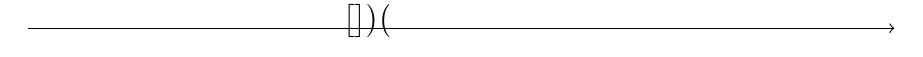
\begin{tikzpicture}
				\draw[->](-4,0)->(7,0);
				\IntervalLR{-4}{-3}
				\IntervalGR{}{}{\big[}{-3}
				\IntervalLR{6}{6.9}
				\IntervalGR{\big]}{6}{}{}
				\IntervalLR{-2}{3}
				\def\skipInterval{0.5cm}
				\IntervalGLF{\big)}{-2}{\big(}{3}
			\end{tikzpicture}
		\end{center}
		Từ hình vẽ, ta có
		Khi đó: $M\cap N= [-3;-2)\cup (3;6]$.}
\end{ex}

\begin{ex}%[Phan Quốc Trí, Bai Giảng T10(2022)]%%[Trần Ngọc Minh]%[301-320-Huỳnh Thanh Tiến]%[0D1B4-1]
	Tập hợp $(1;2)\cap\mathbb{N}$ là tập hợp nào sau đây?
	\choice
	{$\{1;2\}$}
	{$\{1\}$}
	{\True $\varnothing$}
	{$\{2\}$}
	\loigiai{
		Ta có $\mathbb{N}=\{0,1,2,\ldots\}$.
		Do đó 	$(1;2)\cap\mathbb{N}=\varnothing$.
	}
\end{ex}	
\begin{ex}%[Phan Quốc Trí, Bai Giảng T10(2022)]%[0D1B4-1]
	Cho $A=(-5;1]$, $B=[3;+\infty)$, $C=(-\infty;-2)$. Khẳng định nào sau đây đúng?
	\choice
	{$A\cap C=[-5;-2]$}
	{$A\cup B=(-5;+\infty)$}
	{$B\cup C=(-\infty;+\infty)$}
	{$\True B\cap C= \varnothing$}
	\loigiai{
		\begin{center}
			\begin{tikzpicture}
				\draw[->](-1,0)->(5,0);
				\IntervalLR{-1}{3}
				\def\skipInterval{0.5cm}
				\IntervalGRF{}{}{\big[}{3}
				\IntervalLR{4}{4.8}
				\def\skipInterval{0.5cm}
			\end{tikzpicture}\\
			\begin{tikzpicture}
				\draw[->](-1,0)->(5,0);
				\IntervalLR{-1}{1/2}
				\def\skipInterval{0.5cm}
				\IntervalLR{2}{4.9}
				\def\skipInterval{0.5cm}
				\IntervalGRF{\big)}{-2}{}{}
			\end{tikzpicture}
		\end{center}
		Từ biểu diễn tập nghiệm của $B$ và $C$ ta thấy $B\cap C= \varnothing$.
	}
\end{ex}
\begin{ex}%[Phan Quốc Trí, Bai Giảng T10(2022)]%%[0-HK2-2021, Trường THPT Trần Phú, Hải Phòng, năm học 2017 - 2018]%[Trần Quang Thạnh]%[0D1Y4-2]
	Cho tập hợp $A=[-2;3]$ và $B=(-2;5]$. Khi đó $A\setminus B$ là
	\choice
	{$[-2;5] $}
	{$(-2;-1) $}
	{$(3;5) $}
	{\True $\left\{-2\right\} $}
	\loigiai{
		Ta có $A\setminus B=\left\{-2\right\}$.
	}
\end{ex}
\begin{ex}%[Phan Quốc Trí, Bai Giảng T10(2022)]%[0D1B4-2]
	Cho các tập $A=\left\{x\in\mathbb{R}\mid x\ge -1\right\}$; $B=\left\{x\in\mathbb{R}\mid x<3\right\}$. Tập hợp $\mathbb{R}\setminus\left(A\cap B\right)$ là
	\choice
	{$[-1;3)$}
	{$(-\infty;-1]\cup(3;+\infty)$}
	{\True $(-\infty;-1)\cup[3;+\infty)$}
	{$(-1;3]$}
	\loigiai{
		Ta có $A\cap B=[-1;3)$, suy ra $\mathbb{R}\setminus\left(A\cap B\right)=(-\infty;-1)\cup[3;+\infty)$.
	}
\end{ex}
\begin{ex}%[Phan Quốc Trí, Bai Giảng T10(2022)]%[0D1K2-2]
	Tìm tất cả các giá trị của $m$ để đoạn $[m;m+3]$ là tập con của nửa khoảng $(-2;9]$.
	\choice
	{$-2\le m\le 6$}
	{$-2\le m<6$}
	{\True $-2<m\le 6$}
	{$-2<m<6$}
	\loigiai{
		Đoạn $[m;m+3]$ là tập con của nửa khoảng $(-2;9]$ khi và chỉ khi $\heva{& -2<m \\& m+3\le 9}\Leftrightarrow \heva{& -2<m \\& m\le 6}\Leftrightarrow -2<m\le 6.$
	}
\end{ex}



\noindent\textbf{II. PHẦN TỰ LUẬN}
\begin{bt}%[Phan Quốc Trí, Bai Giảng T10(2022)]%[0D1B4-1] 
	Cho $A=\left \{x \in \mathbb{R} \Big|  x \geq 3\right \}$ và $B=(-2 ; 7]$.  Tìm các tập hợp $A \cap B$, $A \cup B$.
	\loigiai{
		Ta có $A=\left \{x \in \mathbb{R} \Big|  x \geq 3\right \} = [3;+\infty )$. \\
		$A \cap B =[3;+\infty ) \cap (-2 ; 7] =    [3;7 ]$. \\
		$A \cup B = [3;+\infty ) \cup (-2 ; 7] = (-2;+\infty)$. 
	}
\end{bt}
\begin{bt}%[Phan Quốc Trí, Bai Giảng T10(2022)]%[0D1B3-2]
	Cho hai tập hợp $A=\left\{ 0;2 \right\}$ và $B=\left\{ 0;1;2;3;4 \right\}$. Tìm tất cả các tập hợp $X$ thỏa mãn $A\cup X=B$.
	\loigiai { 
		Vì $A\cup X=B$ nên $X$ chắc chắn có chứa các phần tử $1;3;4$\\
		Các tập $X$ có thể là $\left\{ 1;3;4 \right\},\,\left\{ 1;3;4;0 \right\},\,\left\{ 1;3;4;2 \right\},\,\left\{ 1;3;4;0;2 \right\}$}
\end{bt}
\begin{bt}%[Phan Quốc Trí, Bai Giảng T10(2022)]%[0D1K4-1]
	Cho hai tập hợp $A=(2m-1;m+3)$, $B=(-4;5)$. Tìm $m$ để
 $A\cap B=\varnothing $.
	\loigiai{
		Điều kiện: $2m-1<m+3 \Leftrightarrow m<4$.\\
	 Ta có  $A\cap B=\varnothing $ khi và chỉ khi $\left[
			\begin{aligned}
				&m+3\leqslant -4\\
				&2m-1\geqslant 5
			\end{aligned}\right. \Leftrightarrow \left[
			\begin{aligned}
				&m\leqslant -7\\
				&m\geqslant 3.
			\end{aligned}\right. $\\
			Đối chiếu điều kiện, ta được $m\leqslant -7$ hoặc $3\leqslant m<4$ thỏa yêu cầu bài toán.
	}
\end{bt}
\begin{bt}%[Phan Quốc Trí, Bai Giảng T10(2022)]%[0D1B3-3]
Lớp 10A có $45$ học sinh, trong đó có $18$ học sinh tham gia cuộc thi vẽ đồ họa trên máy tính, $24$ học sinh tham gia cuộc thi tin học văn phòng cấp trường và $9$ học sinh không tham gia cả hai cuộc thi này. Hỏi lớp 10A có bao nhiêu học sinh tham gia đồng thời cả hai cuộc thi?	
	\loigiai{
\immini{
Gọi $A$ là tập hợp các học sinh tham gia cuộc thi vẽ đồ họa trên máy tính. Suy ra $n(A)= 18$.\\
$B$ là tập hợp các học sinh tham gia  cuộc thi tin học văn phòng cấp trường. Suy ra $n(B)= 24$.\\
Ta có $A \cap B$ là tập hợp các học sinh tham gia đồng thời cả hai cuộc thi.\\
 $A \cup B$ là tập hợp các học sinh tham gia cuộc thi vẽ đồ họa trên máy tính hoặc tham gia  cuộc thi tin học văn phòng cấp trường. 
}{
	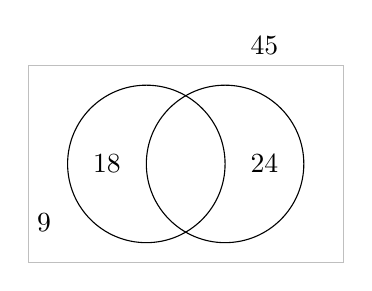
\begin{tikzpicture}
		\draw[] (0,0) circle ( 1.0cm);
		\draw (1.0,0) circle ( 1.0 cm);
		\draw (-0.5,0) node {$18$};
		\draw (1.5,0) node {$24$};
		\draw (-1.3,-0.75) node {$9$};
		\draw (1.5,1.5) node {$45$};
		\node[rectangle,
		draw = lightgray,
		minimum width = 4cm, 
		minimum height = 2.5cm] (r) at (0.5,0) {};
	\end{tikzpicture}
}
$$n \left(A \cup B \right)= 45-9=36.$$	
$$n \left( A \cap B \right) = n(A)+ n(B)-n(A \cup B)=18+24-36= 6.$$
Vậy có $6$  học sinh tham gia đồng thời cả hai cuộc thi.
	}
\end{bt}
\Closesolutionfile{ans}

\newpage
\begin{indapan}{10}
{ans/ans-KT-101}
\end{indapan}

\section*{Đề kiểm tra Chương 1}
\subsection*{Đề số 2}
\setcounter{ex}{0}\setcounter{bt}{0}
\Opensolutionfile{ans}[ans/ans-KT-102]
\noindent\textbf{I. PHẦN TRẮC NGHIỆM}
%[Thi thử, Sở GD và ĐT - Điện Biên, 2018]%[Dương BùiĐức, 12EX10]%[2D2Y3-2]
\begin{ex}%[Phan Quốc Trí, Bai Giảng T10(2022)]%[0D1Y1-1]
	Trong các câu sau, câu nào không phải là mệnh đề?
	\choice
	{Hình bình hành có bốn cạnh bằng nhau}
	{\True Chúc bạn may mắn}
	{Số $8$ là số chính phương}
	{Cà Mau là tên một tỉnh của nước Việt Nam}
	\loigiai{
		Mệnh đề là một câu khẳng định \textbf{đúng} hoặc một câu khẳng định \textbf{sai}.
	}
\end{ex}
\begin{ex}%[Phan Quốc Trí, Bai Giảng T10(2022)]%[0D1Y1-1]
	Trong các câu sau, câu nào là mệnh đề?
	\choice
	{$x^2+x=2$}
	{Hôm nay trời đẹp quá!}
	{$2n+1$ chia hết cho 3}
	{\True Số 15 là một số nguyên tố}
	\loigiai{
		\begin{itemize}
			\item $x^2+x=2$  là một khẳng định, nhưng không là mệnh đề. 
			\item  Hôm nay trời đẹp quá! không phải là mệnh đề.
			\item Câu $2n+1$ chia hết cho 3 là một khẳng định, nhưng không là mệnh đề. 
			\item  Số 15 là một số nguyên tố là một mệnh đề sai.
		\end{itemize}
	}
\end{ex}
\begin{ex}%[Phan Quốc Trí, Bai Giảng T10(2022)]%[0D1Y1-2]
	Trong các mệnh đề sau, mệnh đề nào là mệnh đề \textbf{sai}?
	\choice
	{\True $\sqrt{3}$ là số nguyên}
	{$6$ chia hết cho $2$}
	{$5$ chia hết cho $5$}
	{$30$ là một số chẵn}
	\loigiai{
		Trong các mệnh đề đã cho, mệnh đề sai là \lq\lq$\sqrt{3}$ là số nguyên\rq\rq.
	}
\end{ex}
\begin{ex}%[Phan Quốc Trí, Bai Giảng T10(2022)]%[0D1Y1-2]
	Cho mệnh đề chứa biến $P(x): 3x+5\le x^2$ với $x$ là số thực. Mệnh đề nào sau đây là đúng?
	\choice
	{$P(3)$}
	{$P(4)$}
	{$P(1)$}
	{\True $P(5)$}
	\loigiai{
		$P(3)= 3.3+5\leqslant 3^2 \Leftrightarrow 14\leqslant 9$ là mệnh đề sai.\\
		$P(4) =3.4+5\leqslant 4^2 \Leftrightarrow 17\leqslant 16$ là mệnh đề sai.\\
		$P(1)=3.1+5\leqslant 1^2 \Leftrightarrow 8\leqslant 1$ là mệnh đề sai.\\
		$P(5) =3.5+5\leqslant 5^2 \Leftrightarrow 20\leqslant 25$ là mệnh đề đúng.}
\end{ex}
\begin{ex}%[Phan Quốc Trí, Bai Giảng T10(2022)]%[0D1Y1-3]
	Cho mệnh đề $P\colon$ \lq\lq  $9$ là số chia hết cho $3$\rq\rq. Mệnh đề phủ định của mệnh đề $P$ là
	\choice
	{$\overline{P}\colon$\lq\lq  $9$ là ước của $3$\rq\rq}
	{$\overline{P}\colon$\lq\lq  $9$ là bội của $3$\rq\rq}
	{\True $\overline{P}\colon$ \lq\lq  $9$ là số không chia hết cho $3$\rq\rq}
	{$\overline{P}\colon$\lq\lq  $9$ là số lớn hơn $3$\rq\rq}
	\loigiai{Mệnh đề $P\colon$\lq\lq  $9$ là số chia hết cho $3$\rq\rq      có mệnh đề phủ định là $\overline{P}\colon$ \lq\lq  $9$ là số không chia hết cho $3$\rq\rq.}
\end{ex}
\begin{ex}%[Phan Quốc Trí, Bai Giảng T10(2022)]%[0D1Y1-3]
	Cho mệnh đề \lq\lq$\forall x\in \mathbb{R},\, x^2+1>0$\rq \rq. Mệnh đề phủ định của mệnh đề đã cho là
	\choice
	{\lq\lq$\forall x\in \mathbb{R},\, x^2+1\leq 0$\rq \rq}
	{\lq\lq$\forall x\in \mathbb{R},\, x^2+1<0$\rq \rq}
	{\True \lq\lq$\exists x\in \mathbb{R},\, x^2+1\leq 0$\rq \rq}
	{\lq\lq$\exists x\in \mathbb{R},\, x^2+1>0$\rq \rq}
	\loigiai{
		Mệnh đề phủ định của mệnh đề \lq\lq$\forall x\in \mathbb{R},\, x^2+1>0$\rq \rq\, là \lq\lq$\exists x\in \mathbb{R},\, x^2+1\leq 0$\rq \rq.}
\end{ex}
\begin{ex}%[Phan Quốc Trí, Bai Giảng T10(2022)]%[0D1Y1-4]
	Cho mệnh đề $P\colon$ ``Tam giác $ABC$ cân tại $A$'', mệnh đề $Q\colon$ ``$AB=AC$''. Phát biểu mệnh đề ``$P$ kéo theo $Q$'' là
	\choice
	{Nếu $AB=AC$ thì tam giác $ABC$ cân tại $A$}
	{\True Nếu tam giác $ABC$ cân tại $A$ thì $AB=AC$}
	{Tam giác $ABC$ cân tại $B$ là điều kiện cần và đủ để $AB=AC$}
	{Tam giác $ABC$ cân tại $A$ khi và chỉ khi $AB=AC$}
	\loigiai{
		Mệnh đề ``$P$ kéo theo $Q$'' là ``Nếu tam giác $ABC$ cân tại $A$ thì $AB=AC$''.
	}
\end{ex}
\begin{ex}%[Phan Quốc Trí, Bai Giảng T10(2022)]%[0D1Y1-4]
	Cho mệnh đề $P$: \lq\lq Nếu tam giác có hai đường trung tuyến bằng nhau thì đó là tam giác cân\rq\rq. Mệnh đề nào sau đây là mệnh đề đảo của $P$?
	\choice
	{Tam giác có hai đường trung tuyến bằng nhau thì nó là tam giác cân}
	{\True Nếu tam giác $ABC$ cân thì tam giác đó có hai đường trung tuyến bằng nhau }
	{Tam giác là tam giác cân khi và chỉ khi nó có hai đường trung tuyến bằng nhau}
	{Tam giác là tam giác cân nếu nó có hai đường trung tuyến bằng nhau}
	\loigiai{
		Mệnh đề đảo là \lq \lq Nếu tam giác $ABC$ cân thì tam giác đó có hai đường trung tuyến bằng nhau.\rq \rq		
	}
\end{ex}
\begin{ex}%[Phan Quốc Trí, Bai Giảng T10(2022)]%[0D1Y1-5]
	Mệnh đề "Bình phương mọi số thực đều không âm" mô tả mệnh đề nào dưới đây?
	\choice
	{"$\forall n\in\mathbb{N}: n^2\geq 0$"}
	{"$\exists x\in\mathbb{R}:x^2\geq 0$"}
	{\True "$\forall x\in\mathbb{R}: x^2\geq 0$"}
	{"$\forall x\in\mathbb{R}:x^2>0$"}
	\loigiai{
		Mệnh đề trên được viết lại dạng: \lq \lq $\forall x\in\mathbb{R}: x^2\geq 0$\rq \rq	
	}
\end{ex}
\begin{ex}%[Phan Quốc Trí, Bai Giảng T10(2022)]%[0D1B1-5]
	Mệnh đề nào sau đây là đúng?
	\choice
	{$\forall n\in\mathbb{N}\colon n^2>n$}
	{$\forall x\in\mathbb{R}\colon x^2<2$}
	{$\forall x\in\mathbb{Z}\colon 2x>1$}
	{\True $\exists x\in\mathbb{R}\colon x^2>x$}
	\loigiai
	{
		\begin{itemize}
			\item Mệnh đề ``$\forall n\in\mathbb{N}\colon n^2>n$'' sai vì với $n=1$ thì $n^2=1=n$.
			\item Mệnh đề ``$\forall x\in\mathbb{R}\colon x^2<2$'' sai vì với $x=2$ thì $x^2=4>2$.
			\item Mệnh đề ``$\forall x\in\mathbb{Z}\colon 2x>1$'' sai vì với $x=0$ thì $2x=0<1$.
			\item Mệnh đề ``$\exists x\in\mathbb{R}\colon x^2>x$'' đúng vì với $x=2$ thì $x^2=4$ nên $x^2>x$.
		\end{itemize}
	}
\end{ex}
\begin{ex}%[Phan Quốc Trí, Bai Giảng T10(2022)]%[0D1Y2-1]
	Hãy liệt kê các phần tử của tập hợp $X = \left\{ x \in \mathbb{Z} | 2x^2-5x+3=0 \right\}$.
	\choice
	{$X = \left\{1;\dfrac{3}{2} \right\}$}
	{\True $X = \{ 1 \}$}
	{$X = \left\{ \dfrac{3}{2} \right\}$}
	{$X = \varnothing$}
	\loigiai{
		Ta có $2x^2-5x+3=0\Leftrightarrow \hoac{&x=1\in \mathbb{Z}\\&x=\dfrac{3}{2}\notin \mathbb{Z}}$.\\
		Vậy $X = \{ 1 \}$.		
	}
\end{ex}
\begin{ex}%[Phan Quốc Trí, Bai Giảng T10(2022)]%[0D1B2-1]
	Viết tập hợp $A=\lbrace x \in \mathbb{Z}|x^2<17 \rbrace $ theo cách liệt kê các phần tử, ta được tập hợp nào sau đây?
	\choice{\True $ \lbrace -4;-3;-2;-1;0;1;2;3;4 \rbrace $}
	{$ \lbrace 1;2;3;4 \rbrace $}
	{$\lbrace 0;1;2;3;4  \rbrace $}
	{$ \lbrace -4; -3;-2;-1 \rbrace $}
	\loigiai{Ta có $x^2<17\Leftrightarrow \left|x\right|<\sqrt{17}\Leftrightarrow -\sqrt{17}<x<\sqrt{17}$.\\
		Vì $x\in \mathbb{Z}$ nên $A=\lbrace -4;-3;-2;-1;0;1;2;3;4 \rbrace $.
	}
\end{ex}

\begin{ex}%[Phan Quốc Trí, Bai Giảng T10(2022)]%[0D1Y2-1]
	Cho tập hợp $A=\left\{ x \in \mathbb{N}| x^2+2x-3=0 \right\}$. Mệnh đề nào sau đây là đúng?
	\choice
	{\True $-3 \notin A$}
	{$A=\left\{1;-3\right\}$}
	{$1 \notin A$}
	{$A=\left\{1;3\right\}$}
	\loigiai{
		Ta có $x^2+2x-3=0 \Leftrightarrow \hoac{&x=1\\&x=-3}$. Do $x \in \mathbb{N}$ nên $A=\left\{1\right\}$. Do đó $-3 \notin A$.
	}
\end{ex}
\begin{ex}%[Phan Quốc Trí, Bai Giảng T10(2022)]%[0D1Y2-2]
	Cho tập $A=\{a;b;5\}$. Số tập con của tập $A$ là
	\choice
	{$5$}
	{\True $8$}
	{$7$}
	{$4$}
	\loigiai{Tập con của $A$ là $\varnothing, \{a\}, \{b\},\{5\}, \{a;b\}, \{a;5\}, \{b;5\}, \{a;b;5\} $. Vậy số tập con của $A$ là $8$.
	}
\end{ex}
\begin{ex}%[Phan Quốc Trí, Bai Giảng T10(2022)]%[0D1Y2-2]
	Có bao nhiêu tập $ X $ thỏa mãn $ \{a;b\} \subset X \subset \{1;2;a;b\}$?
	\choice
	{$3$}
	{$2$}
	{\True $4$}
	{$5$}
	\loigiai{
		Các tập $ X $ thỏa mãn là $ \{a;b\} $, $ \{1;a;b\} $, $ \{2;a;b\} $, $ \{1;2;a;b\} $.
	}
\end{ex}
\begin{ex}%[Phan Quốc Trí, Bai Giảng T10(2022)]%[0D1B4-1]
	Cho tập hợp $A=\{x\in\mathbb{R}|-3<x\le 3\}$. Mệnh đề nào dưới đây đúng?
	\choice
	{$A=\{-2;-1;0;1;2;3\}$}
	{\True $A=(-3;3]$}
	{$A=[-3;3]$}
	{$A=[-3;3)$}
	\loigiai{
		Từ giả thiết, có $A=(-3;3]$.
	}
\end{ex}
\begin{ex}%[Phan Quốc Trí, Bai Giảng T10(2022)]%[0D1B2-2]
	Cho tập hợp $A = \left\{x \in \mathbb{N}\big| x^2 + 8x + 15 = 0\right\}$. Khẳng định nào sau đây đúng?
	\choice
	{$A = \left\{-3;-5\right\}$}
	{\True $A =\varnothing$}
	{$A = \left\{\varnothing\right\}$}
	{$A = \left\{0\right\}$}
	\loigiai{
		Phương trình $x^2+8x+15=0$ có hai nghiệm $x_1=-3$, $x_2=-5$. Tuy nhiên $x_1, x_2\notin \mathbb{N}$. Vậy $A=\varnothing$.
	}
\end{ex}
\begin{ex}%[Phan Quốc Trí, Bai Giảng T10(2022)]%[0D1B2-2]
	Gọi $A$ là tập hợp tất cả các hình bình hành và $B$ là tập hợp tất cả các hình chữ nhật. Trong các kết luận sau, kết luận nào đúng?
	\choice
	{$A \subset B$}
	{\True $B \subset A$}
	{$A=B$}
	{$A \cap B=\varnothing$}
	\loigiai{
		Ta có hình chữ nhật là hình bình hành có một góc vuông nên $B \subset A$.
	}
\end{ex}

\begin{ex}%[Phan Quốc Trí, Bai Giảng T10(2022)]%[0D1Y2-2]
	Khẳng định nào sau đây là đúng?
	\choice
	{$ \mathbb{R}\subset\mathbb{Q} $}
	{$ \mathbb{Z}\subset\mathbb{N} $}
	{$ \mathbb{Q}\subset\mathbb{Z} $}
	{\True $ \mathbb{N}\subset\mathbb{R} $}
	\loigiai{
		Ta có $ \mathbb{N}\subset\mathbb{Z}\subset\mathbb{Q}\subset\mathbb{R} $.
	}
\end{ex}
\begin{ex}%[Phan Quốc Trí, Bai Giảng T10(2022)]%[0D1Y3-1]
	Cho hai tập hợp $X=\left\{1;3;5;8\right\}$ và $Y=\left\{3;5;7;9\right\}$. Tập hợp $X\cup Y$ bằng
	\choice
	{$\left\{1;7;9\right\}$}
	{$\left\{3;5\right\}$}
	{$\left\{1;3;5\right\}$}
	{\True $\left\{1;3;5;7;8;9\right\}$}
	\loigiai{
		Ta có $X\cup Y=\left\{1;3;5;7;8;9\right\}$.
	}
\end{ex}
\begin{ex}%[Phan Quốc Trí, Bai Giảng T10(2022)]%[0D1Y3-1]
	Cho $A=\{2;3;6;7\}, B=\{3;6;8\}$. Tập hợp $A\cap B$ bằng
	\choice
	{$\{3;6;8\}$}
	{$\{2;3;6;7;8\}$}
	{\True $\{3;6\}$}
	{$\{2;7\}$}
	\loigiai{
		Ta có $A\cap B=\{3;6\}.$
	}
\end{ex}
\begin{ex}%[Phan Quốc Trí, Bai Giảng T10(2022)]%[0D1Y3-2]
	Cho hai tập hợp $A=\{2;4;6;9\}$, $B=\{1;2;3;4\}$. Tập $A \setminus B$ bằng tập hợp nào sau đây?
	\choice
	{$\{2;4\}$}
	{$\{1;3\}$}
	{\True $\{6;9\}$}
	{$\{6;9;1;3\}$}
	\loigiai{
		Ta có: $A \setminus B=\{6;9\}$.}
\end{ex}

\begin{ex}%[Phan Quốc Trí, Bai Giảng T10(2022)]%[0D1Y3-2] 
	Cho tập $ X=\left\lbrace 0;1;2;3;4;5 \right\rbrace$ và tập $ A=\left\lbrace 0;2;4 \right\rbrace  $. Tìm phần bù của $ A $ trong $ X $.	
	\choice
	{$ \varnothing $}
	{$ \left\lbrace 2;4 \right\rbrace $ }
	{$ \left\lbrace 0;1;3 \right\rbrace  $}
	{\True $ \left\lbrace 1;3;5 \right\rbrace  $}
	\loigiai
	{
		Ta có phần bù của $ A $ trong $ X $ bằng tập $ X\setminus A=\left\lbrace 1;3;5 \right\rbrace  $.	
	}
\end{ex}
\begin{ex}%[Phan Quốc Trí, Bai Giảng T10(2022)]%[0D1B3-1]
	Cho hai tập hợp $A=(-3;3)$ và $B=(0;+\infty)$. Tìm  $A \cup B$.
	\choice
	{\True $ A \cup B = (-3;+\infty) $}
	{$ A \cup B = [-3;+\infty) $}
	{$ A \cup B = [-3;0) $}
	{$ A \cup B = (0;3) $}
	\loigiai{
		\immini{Tập hợp $A=(-3;3)$ có biểu diễn là}{ 
			\begin{tikzpicture}[scale=1, font=\footnotesize, line join = round, line cap = round, >=stealth]
				\draw[thick,->] (-2,0)node[below=6pt]{$-\infty$} -- (0,0) node[scale=1.5]{\bf ( } node[below=6pt]{$-3$} -- (3,0) node[scale=1.5]{\bf )} node[below=6pt]{$3$} -- (5,0)node[below=6pt]{$+\infty$};
				\foreach \i in {1,...,10} 
				\draw ($(0,0)-(.2*\i,0)$) node[scale=.6]{/};
				\draw ($(0,0)$) node[scale=.6]{/};
				\foreach \i in {1,...,9} 
				\draw ($(3,0)+(.2*\i,0)$) node[scale=.6]{/};
				\draw ($(3,0)$) node[scale=.6]{/};
		\end{tikzpicture}}
		\immini{Tập hợp $B=(0;+\infty)$ có biểu diễn là}{
			\begin{tikzpicture}[scale=1, font=\footnotesize, line join = round, line cap = round, >=stealth]
				\draw[thick,->] (-2,0)node[below=6pt]{$-\infty$}--(1,0) node[scale=1.5]{\bf (} node[below=6pt]{$0$}-- (5,0)node[below=6pt]{$+\infty$};
				\foreach \i in {1,...,15} 
				\draw ($(1,0)-(.2*\i,0)$) node[scale=.6,rotate=60]{/};
				\draw ($(1,0)$) node[scale=.6,rotate=60]{/};
				%	\foreach \i in {1,...,5} 
				%	\draw ($(4,0)+(.2*\i,0)$) node[scale=.6,rotate=60]{/};
		\end{tikzpicture}}
		\noindent Do đó $A \cup B=(-3;+\infty)$.
	}
\end{ex}
\begin{ex}%[Phan Quốc Trí, Bai Giảng T10(2022)]%[0D1B3-1]
	Cho tập hợp $X=(-\infty;2] \cap (-6;+\infty)$. Khẳng định nào sau đây là đúng?
	\choice
	{\True $X=(-6;2]$}
	{$(-6;+\infty)$}
	{$X=(-\infty;+\infty)$}
	{$X=(-\infty;2]$}
	\loigiai{
		Ta có: $X=(-\infty;2] \cap (-6;+\infty)=(-6;2]$.}
\end{ex}

\begin{ex}%[Phan Quốc Trí, Bai Giảng T10(2022)]%[0D1B3-2]
	Cho tập hợp $ A=[-2;3] $ và $ B=(1;5] $. Khi đó $ A\setminus B $ là
	\choice
	{$(-2;1]$}
	{$(-2;-1)$}
	{$[-2;1) $}
	{\True $[-2;1]$}
	\loigiai{
		Ta có $ A\setminus B =[-2;3]\setminus(1;5]= [-2;1]$. 
	}
\end{ex}

\begin{ex}%[Phan Quốc Trí, Bai Giảng T10(2022)]%[0D1B3-2]
	Cho tập hợp $A=\left\{x \in \mathbb{R} |  0 \le x+2 <5 \right\}$. Tập hợp $C_{\mathbb{R}}A$ bằng
	\choice
	{$(-\infty;-2)$}
	{$(-\infty;-2] \cup (3;+\infty)$}
	{\True $(-\infty;-2) \cup [3;+\infty)$}
	{$[3;+\infty)$}
	\loigiai{
		Ta có: $C_{\mathbb{R}}A=(-\infty;-2) \cup [3;+\infty)$.}
\end{ex}
\begin{ex}%[Phan Quốc Trí, Bai Giảng T10(2022)]%[0D1B3-3]
	Một lớp học có $25$ học sinh giỏi môn Toán, $23$ học sinh giỏi môn Lý, $14$ học sinh giỏi cả môn Toán và Lý và có $6$ học sinh không giỏi môn nào cả. Hỏi lớp đó có bao nhiêu học sinh?
	\choice
	{$26$}
	{$54$}
	{$68$}
	{\True $40$}
	\loigiai
	{
		Vì có $25$ học sinh giỏi môn Toán và $14$ học sinh giỏi cả môn Toán và Lý nên có $25-14=11$ học sinh chỉ giỏi môn Toán mà không giỏi môn Lý. \\
		Vì có $23$ học sinh giỏi môn Lý và $14$ học sinh giỏi cả môn Toán và Lý nên có $23-14=9$ học sinh chỉ giỏi môn Lý mà không giỏi môn Toán. \\
		Vậy lớp đó có $11+9+14+6=40$ học sinh.
	}
\end{ex}
\begin{ex}%[Phan Quốc Trí, Bai Giảng T10(2022)]%[0D1B3-3]
	Mỗi học sinh của lớp $10A$ đều chơi bóng đá hoặc bóng chuyền. Biết rằng có $25$ bạn chơi bóng đá, $20$ bạn chơi bóng chuyền và $10$ bạn chơi cả $2$ môn thể thao. Hỏi lớp $10A$ có bao nhiêu học sinh.
	\choice
	{$30$}
	{$55$}
	{$45$}
	{\True $35$}
	\loigiai{
		Ngoài sơ đồ Ven ta có thể dùng công thức số phần tử. Gọi $A$ là tập hợp các học sinh chơi bóng đá, $B$ là tập các học sinh chơi bóng chuyền. Do đó $A\cap B$ là tập các học sinh chơi cả hai môn. Ta có
		$$|A|=25, |B|=20, |A \cap B| =10.$$
		Số học sinh cả lớp là số phần tử của tập $A \cup B$. Theo công thức ta có $|A \cup B| = 25+20-10=35$ (học sinh).
	}
\end{ex}
\begin{ex}%[Phan Quốc Trí, Bai Giảng T10(2022)]%[0D1B3-1] 
	Cho các tập hợp $M=[-3;6]$ và $N=(-\infty; -2)\cup (3;+\infty)$. Khi đó $M\cap N$ là
	\choice
	{$(-\infty;-2)\cup (3;6)$}
	{$(-\infty;-2)\cup [3;+\infty)$}
	{\True $[-3;-2)\cup (3;6]$}
	{$(-3;-2)\cup (3;6)$}
	\loigiai{
		Biểu diễn trục số:  
		\begin{center}
			\begin{tikzpicture}
				\draw[->](-4,0)->(7,0);
				\IntervalLR{-4}{-3}
				\IntervalGR{}{}{\big[}{-3}
				\IntervalLR{6}{6.9}
				\IntervalGR{\big]}{6}{}{}
				\IntervalLR{-2}{3}
				\def\skipInterval{0.5cm}
				\IntervalGLF{\big)}{-2}{\big(}{3}
			\end{tikzpicture}
		\end{center}
		Từ hình vẽ, ta có
		Khi đó: $M\cap N= [-3;-2)\cup (3;6]$.}
\end{ex}


\begin{ex}%[Phan Quốc Trí, Bai Giảng T10(2022)]%%[Trần Ngọc Minh]%[301-320-Huỳnh Thanh Tiến]%[0D1B4-1]
	Tập hợp $(1;2)\cap\mathbb{N}$ là tập hợp nào sau đây?
	\choice
	{$\{1;2\}$}
	{$\{1\}$}
	{\True $\varnothing$}
	{$\{2\}$}
	\loigiai{
		Ta có $\mathbb{N}=\{0,1,2,\ldots\}$.
		Do đó 	$(1;2)\cap\mathbb{N}=\varnothing$.
	}
\end{ex}	
\begin{ex}%[Phan Quốc Trí, Bai Giảng T10(2022)]%[0D1B4-1]
	Cho $A=(-5;1]$, $B=[3;+\infty)$, $C=(-\infty;-2)$. Khẳng định nào sau đây đúng?
	\choice
	{$A\cap C=[-5;-2]$}
	{$A\cup B=(-5;+\infty)$}
	{$B\cup C=(-\infty;+\infty)$}
	{$\True B\cap C= \varnothing$}
	\loigiai{
		\begin{center}
			\begin{tikzpicture}
				\draw[->](-1,0)->(5,0);
				\IntervalLR{-1}{3}
				\def\skipInterval{0.5cm}
				\IntervalGRF{}{}{\big[}{3}
				\IntervalLR{4}{4.8}
				\def\skipInterval{0.5cm}
			\end{tikzpicture}\\
			\begin{tikzpicture}
				\draw[->](-1,0)->(5,0);
				\IntervalLR{-1}{1/2}
				\def\skipInterval{0.5cm}
				\IntervalLR{2}{4.9}
				\def\skipInterval{0.5cm}
				\IntervalGRF{\big)}{-2}{}{}
			\end{tikzpicture}
		\end{center}
		Từ biểu diễn tập nghiệm của $B$ và $C$ ta thấy $B\cap C= \varnothing$.
	}
\end{ex}
\begin{ex}%[Phan Quốc Trí, Bai Giảng T10(2022)]%%[0-HK2-2021, Trường THPT Trần Phú, Hải Phòng, năm học 2017 - 2018]%[Trần Quang Thạnh]%[0D1Y4-2]
	Cho tập hợp $A=[-2;3]$ và $B=(-2;5]$. Khi đó $A\setminus B$ là
	\choice
	{$[-2;5] $}
	{$(-2;-1) $}
	{$(3;5) $}
	{\True $\left\{-2\right\} $}
	\loigiai{
		Ta có $A\setminus B=\left\{-2\right\}$.
	}
\end{ex}
\begin{ex}%[Phan Quốc Trí, Bai Giảng T10(2022)]%[0D1B4-2]
	Cho các tập $A=\left\{x\in\mathbb{R}\mid x\ge -1\right\}$; $B=\left\{x\in\mathbb{R}\mid x<3\right\}$. Tập hợp $\mathbb{R}\setminus\left(A\cap B\right)$ là
	\choice
	{$[-1;3)$}
	{$(-\infty;-1]\cup(3;+\infty)$}
	{\True $(-\infty;-1)\cup[3;+\infty)$}
	{$(-1;3]$}
	\loigiai{
		Ta có $A\cap B=[-1;3)$, suy ra $\mathbb{R}\setminus\left(A\cap B\right)=(-\infty;-1)\cup[3;+\infty)$.
	}
\end{ex}
\begin{ex}%[Phan Quốc Trí, Bai Giảng T10(2022)]%[0D1B2-2]
	Tìm tất cả các giá trị của $m$ để đoạn $[m;m+3]$ là tập con của nửa khoảng $(-2;9]$.
	\choice
	{$-2\le m\le 6$}
	{$-2\le m<6$}
	{\True $-2<m\le 6$}
	{$-2<m<6$}
	\loigiai{
		Đoạn $[m;m+3]$ là tập con của nửa khoảng $(-2;9]$ khi và chỉ khi $\heva{& -2<m \\& m+3\le 9}\Leftrightarrow \heva{& -2<m \\& m\le 6}\Leftrightarrow -2<m\le 6.$
	}
\end{ex}



\noindent\textbf{II. PHẦN TỰ LUẬN}
\begin{bt}%[Phan Quốc Trí, Bai Giảng T10(2022)]%[0D1B4-1] 
	Cho $A=\left \{x \in \mathbb{R} \Big|  x \geq 3\right \} ; B=(-2 ; 7]$.  Tìm các tập hợp $A \cap B, A \cup B$.
	\loigiai{
		Ta có $A=\left \{x \in \mathbb{R} \Big|  x \geq 3\right \} = [3;+\infty )$. \\
		$A \cap B =[3;+\infty ) \cap (-2 ; 7] =    [3;7 ]$. \\
		$A \cup B = [3;+\infty ) \cup (-2 ; 7] = (-2;+\infty)$. 
	}
\end{bt}
\begin{bt}%[Phan Quốc Trí, Bai Giảng T10(2022)]%[0D1B3-2]
	Cho hai tập hợp $A=\left\{ 0;2 \right\}$ và $B=\left\{ 0;1;2;3;4 \right\}$. Tìm tất cả các tập hợp $X$ thỏa mãn $A\cup X=B$.
	\loigiai { 
		Vì $A\cup X=B$ nên $X$ chắc chắn có chứa các phần tử $1;3;4$\\
		Các tập $X$ có thể là $\left\{ 1;3;4 \right\},\,\left\{ 1;3;4;0 \right\},\,\left\{ 1;3;4;2 \right\},\,\left\{ 1;3;4;0;2 \right\}$}
\end{bt}
\begin{bt}%[Phan Quốc Trí, Bai Giảng T10(2022)]%[0D1B4-1]
	Cho hai tập hợp $A=(2m-1;m+3)$, $B=(-4;5)$. Tìm $m$ để
	$A\cap B=\varnothing $.
	\loigiai{
		Điều kiện: $2m-1<m+3 \Leftrightarrow m<4$.
		Để $A\cap B=\varnothing $ khi và chỉ khi $\left[
		\begin{aligned}
			&m+3\leqslant -4\\
			&2m-1\geqslant 5
		\end{aligned}\right. \Leftrightarrow \left[
		\begin{aligned}
			&m\leqslant -7\\
			&m\geqslant 3
		\end{aligned}\right. $.\\
		Đối chiếu điều kiện, ta được $m\leqslant -7$ hoặc $3\leqslant m<4$ thỏa yêu cầu bài toán.
	}
\end{bt}
\begin{bt}%[Phan Quốc Trí, Bai Giảng T10(2022)]%[0D1B3-3]
	Lớp 10A có $45$ học sinh, trong đó có $18$ học sinh tham gia cuộc thi vẽ đồ họa trên máy tính, $24$ học sinh tham gia cuộc thi tin học văn phòng cấp trường và $9$ học sinh không tham gia cả hai cuộc thi này. Hỏi lớp 10A có bao nhiêu học sinh tham gia đồng thời cả hai cuộc thi?	
	\loigiai{
		\immini{
			Gọi $A$ là tập hợp các học sinh tham gia cuộc thi vẽ đồ họa trên máy tính. Suy ra $n(A)= 18$.\\
			$B$ là tập hợp các học sinh tham gia  cuộc thi tin học văn phòng cấp trường. Suy ra $n(B)= 24$.\\
			Ta có $A \cap B$ là tập hợp các học sinh tham gia đồng thời cả hai cuộc thi.\\
			$A \cup B$ là tập hợp các học sinh tham gia cuộc thi vẽ đồ họa trên máy tính hoặc tham gia  cuộc thi tin học văn phòng cấp trường. 
		}{
			\begin{tikzpicture}
				\draw[] (0,0) circle ( 1.0cm);
				\draw (1.0,0) circle ( 1.0 cm);
				\draw (-0.5,0) node {$18$};
				\draw (1.5,0) node {$24$};
				\draw (-1.3,-0.75) node {$9$};
				\draw (1.5,1.5) node {$45$};
				\node[rectangle,
				draw = lightgray,
				minimum width = 4cm, 
				minimum height = 2.5cm] (r) at (0.5,0) {};
			\end{tikzpicture}
		}
		$$n \left(A \cup B \right)= 45-9=36.$$	
		$$n \left( A \cap B \right) = n(A)+ n(B)-n(A \cup B)=18+24-36= 6.$$
		Vậy có $6$  học sinh tham gia đồng thời cả hai cuộc thi.
	}
\end{bt}

\Closesolutionfile{ans}

\newpage
\begin{indapan}{10}
	{ans/ans-KT-102}
\end{indapan}




\section*{Đề kiểm tra Chương 1}
\subsection*{Đề số 3}
\setcounter{ex}{0}\setcounter{bt}{0}
\Opensolutionfile{ans}[ans/ans-KT-103]
\noindent\textbf{I. PHẦN TRẮC NGHIỆM}
%[Thi thử, Sở GD và ĐT - Điện Biên, 2018]%[Dương BùiĐức, 12EX10]%[2D2Y3-2]
\begin{ex}%[Phan Quốc Trí, Bai Giảng T10(2022)]%[0D1Y1-1]
	Câu nào trong các câu sau \textbf{không phải} là mệnh đề?
	\choice
	{\True $\pi$ có phải là một số vô tỷ không?}
	{$2+2=5$}
	{$\sqrt{2}$ là một số hữu tỷ}
	{$\dfrac{4}{2}=2$}
	\loigiai{
		\lq\lq $\pi$ có phải là một số vô tỷ không?\rq\rq\, là câu hỏi, nên không phải là mệnh đề.
	}
\end{ex}
\begin{ex}%[Phan Quốc Trí, Bai Giảng T10(2022)]%[0D1Y1-1]
	Phát biểu nào sau đây là một mệnh đề?
	\choice
	{Mùa thu Hà Nội đep quá!}
	{\True Hà Nội là thủ đô của Việt Nam}
	{Bạn có đi học không?}
	{Đề thi môn Toán khó quá!}
	\loigiai{
		Hà Nội là thủ đô của Việt Nam là một khẳng định đúng.
	}
\end{ex}
\begin{ex}%[Phan Quốc Trí, Bai Giảng T10(2022)]%[0D1Y1-2]
	Trong các mệnh đề sau, mệnh đề nào \textbf{sai}?
	\choice
	{$-2 \in \mathbb{Q}$}
	{$\sqrt{2} \in \mathbb{R}$}
	{\True $\dfrac{1}{2} \in \mathbb{Z}$}
	{$2 \in \mathbb{N}$}
	\loigiai{
		Mệnh đề sai là  $\dfrac{1}{2} \in \mathbb{Z}$.
	}
\end{ex}
\begin{ex}%[Phan Quốc Trí, Bai Giảng T10(2022)]%[0D1Y1-2]
	Cho mệnh đề chứa biến $P(n) \colon$ "$n^2-1$ chia hết cho $4$" với $n$ là số nguyên. Khẳng định nào sau đây đúng?
	\choice
	{$P(5)$ đúng và $P(2)$ đúng}
	{\True $P(5)$ đúng và $P(2)$ sai}
	{$P(5)$ sai và $P(2)$ sai}
	{$P(5)$ sai và $P(2)$ đúng}
	\loigiai{
		Ta có:\\
		$P(5) \colon$ "$5^2-1$ chia hết cho $4$" tức là "$24$ chia hết cho $4$", nên $P(5)$ đúng.\\
		$P(2) \colon$ "$2^2-1$ chia hết cho $4$" tức là "$3$ chia hết cho $4$", nên $P(2)$ sai.\\
		Vậy $P(5)$ đúng và $P(2)$ đúng.}
\end{ex}
\begin{ex}%[Phan Quốc Trí, Bai Giảng T10(2022)]%[0D1Y1-3]
	Phủ định của mệnh đề: ``$\pi$ là số vô tỷ'' là
	\choice
	{$\pi$ là số nguyên}
	{$\pi$ là số dương}
	{$\pi$ là số thực}
	{\True $\pi$ không phải là số vô tỷ}	
	\loigiai{Mệnh đề phủ định là ``$\pi$ không phải là số vô tỷ''.}
\end{ex}
\begin{ex}%[Phan Quốc Trí, Bai Giảng T10(2022)]%[0D1Y1-3]
	Mệnh đề phủ định của mệnh đề \lq \lq $\exists x\in \mathbb{N}\colon x^2-4=0$\rq \rq \ là
	\choice
	{\lq \lq $\forall x\in \mathbb{N}\colon x^2-4=0$\rq \rq }
	{\lq \lq $\forall x\in \mathbb{N}\colon x^2-4>0$\rq \rq }
	{\lq \lq $\exists x\in \mathbb{N}\colon x^2-4\ne 0$\rq \rq }
	{\True \lq \lq $\forall x\in \mathbb{N}\colon x^2-4\ne 0$\rq \rq}
	\loigiai{
		Ta có mệnh đề phủ định của mệnh đề \lq\lq $\exists x \in X, P(x)$\rq\rq\ là \lq\lq $\forall x \in X, \overline{P(x)}$\rq\rq.\\
		Nên mệnh đề phủ định của mệnh đề \lq \lq $\exists x\in \mathbb{N}\colon x^2-4=0$\rq \rq \ là \lq \lq $\forall x\in \mathbb{N}\colon x^2-4\ne 0$\rq \rq.
	}
\end{ex}
\begin{ex}%[Phan Quốc Trí, Bai Giảng T10(2022)]%[0D1Y1-4]
	Cho mệnh đề $P\colon$ ``$b^2\ge 4ac$'', mệnh đề $Q\colon$ ``Phương trình $ax^2 +bx+c=0$ vô nghiệm'' (với $a,b,c$ là số thực và $a\ne 0$). Phát biểu mệnh đề ``$P$ kéo theo $Q$'' là
	\choice
	{Nếu Phương trình $ax^2 +bx+c=0$ vô nghiệm thì $b^2\ge 4ac$ (với $a,b,c$ là số thực và $a\ne 0$)}
	{\True Nếu $b^2\ge 4ac$ thì phương trình $ax^2 +bx+c=0$ vô nghiệm (với $a,b,c$ là số thực và $a\ne 0$) }
	{$b^2\ge 4ac$ là điều kiện cần và đủ để phương trình $ax^2 +bx+c=0$ vô nghiệm (với $a,b,c$ là số thực và $a\ne 0$)}
	{$b^2\ge 4ac$ khi và chỉ khi phương trình $ax^2 +bx+c=0$ vô nghiệm (với $a,b,c$ là số thực và $a\ne 0$)}
	\loigiai{
		Mệnh đề ``$P$ kéo theo $Q$'' là ``Nếu $b^2\ge 4ac$ thì phương trình $ax^2 +bx+c=0$ vô nghiệm (với $a,b,c$ là số thực và $a\ne 0$)''.
	}
\end{ex}
\begin{ex}%[Phan Quốc Trí, Bai Giảng T10(2022)]%[0D1Y1-4]
	Cho mệnh đề $P$: \lq\lq Nếu tam giác $ABC$ có hai góc bằng $60^{\circ}$ thì đó là tam giác$ABC$ đều\rq\rq. Mệnh đề nào sau đây là mệnh đề đảo của $P$?
	\choice
	{Tam giác $ABC$ có hai góc bằng $60^{\circ}$ thì đó là tam giác$ABC$ đều}
	{\True Nếu tam giác $ABC$ đều thì tam giác đó có hai góc bằng $60^{\circ}$}
	{Tam giác $ABC$ đều khi và chỉ khi tam giác đó có hai góc bằng $60^{\circ}$}
	{Tam giác$ABC$ đều nếu nó có hai góc bằng $60^{\circ}$}
	\loigiai{
		Mệnh đề đảo là \lq \lq Nếu tam giác $ABC$ đều thì tam giác đó có hai góc bằng $60^{\circ}$.\rq \rq		
	}
\end{ex}
\begin{ex}%[Phan Quốc Trí, Bai Giảng T10(2022)]%[0D1Y1-5]
	Mệnh đề "Có ít nhất một số tự nhiên khác 0" mô tả mệnh đề nào dưới đây?
	\choice{"$\forall n\in\mathbb{N}: n\neq 0$"}
	{"$\exists x\in\mathbb{N}:x=0$"}
	{"$\exists x\in\mathbb{Z}: x\neq 0$"}
	{\True "$\exists x\in\mathbb{N}:x\neq 0$"}
	\loigiai{
		Mệnh đề được viết lại là: "$\exists x\in\mathbb{N}:x\neq 0$".}
\end{ex}
\begin{ex}%[Phan Quốc Trí, Bai Giảng T10(2022)]%[0D1Y1-5]
	Mệnh đề nào sau đây đúng?
	\choice{$\forall n\in\mathbb{N}: n > 0$}
	{\True $\exists m\in\mathbb{Z}:2m=m$}
	{$\forall x\in\mathbb{R}:x^2> 0$}
	{$\exists k\in\mathbb{Q}:k^2=2$}
	\loigiai{
		Mệnh đề $\forall n\in\mathbb{N}: n > 0$ là mệnh đề sai, ví dụ $n=0$.\\
		Mệnh đề $\exists m\in\mathbb{Z}:2m=m$ là mệnh đề đúng, vì tồn tại $m=0$ thỏa mãn.\\
		Mệnh đề $\forall x\in\mathbb{R}:x^2> 0$ là mệnh đề sai, ví dụ $x=0$.\\
		Mệnh đề $\exists k\in\mathbb{Q}:k^2=2$ là mệnh đề sai.}
\end{ex}
\begin{ex}%[Phan Quốc Trí, Bai Giảng T10(2022)]%[0D1Y2-1]
	Hãy liệt kê các phần tử của tập $X=\left\{ x \in \mathbb{Q}| (x^2-x-6)(x^2-5)=0 \right\}$.
	\choice
	{$X=\left\{ \sqrt{5};3 \right\}$}
	{\True $X=\left\{ -2;3 \right\}$}
	{$X=\left\{ -\sqrt{5};-2;\sqrt{5}; 3 \right\}$}
	{$X=\left\{ -\sqrt{5};\sqrt{5}  \right\}$}
	\loigiai{
		Ta có 
		\begin{itemize}
			\item $x^2-x-6 = 0 \Leftrightarrow \hoac{&x=3 \in \mathbb{Q} \\&x=-2 \in \mathbb{Q}. }$
			\item $x^2-5 =0 \Leftrightarrow \hoac{&x= \sqrt{5} \notin \mathbb{Q} \\& x= - \sqrt{5} \notin \mathbb{Q}.}$
		\end{itemize}
		Do đó $X=\left\{ -2;3 \right\}$.
	}
\end{ex}
\begin{ex}%[Phan Quốc Trí, Bai Giảng T10(2022)]%[0D1Y2-1]
	Hãy liệt kê các phần tử của tập hợp $X=\left\{x \in \mathbb{N} \ |  \ x \leq 3\right\}$
	\choice
	{$X=\left[0;3\right]$}
	{\True $X=\left\{0;1;2;3\right\}$}
	{$X=\left\{1;2;3\right\}$}
	{$X=\left\{0  \longrightarrow 3\right\}$}
	\loigiai{ 
		Liệt kê các phần tử của tập hợp $X=\left\{x \in \mathbb{N} \ | \ x \leq 3\right\}=\left\{0;1;2;3\right\}$.
	}
\end{ex}

\begin{ex}%[Phan Quốc Trí, Bai Giảng T10(2022)]%[0D1Y2-1]
	Cho tập hợp $A=\{x\in \mathbb{R}|x^2-2x+5=0\}$. Mệnh đề nào sau đây đúng?
	\choice
	{\True $A=\varnothing$}
	{$A=0$}
	{$A=\{-1\}$}
	{$A=\{0\}$}
	\loigiai{
		Vì phương trình $x^2-2x+5=0$ vô ngiệm nên $A=\varnothing$.	
	}	
\end{ex}
\begin{ex}%[Phan Quốc Trí, Bai Giảng T10(2022)]%[0D1Y2-2]
	Cho tập hợp $A=\{a;b;c;d\}$. Số tập hợp con của $A$ có hai phần tử là
	\choice
	{\True $6$}
	{$7$}
	{$8$}
	{$5$}
	\loigiai{
		Sô tập con có hai phần tử của tập $A$ là $6$ đó là các tập $\{a;b\}$, $\{a;c\}$, $\{a;d\}$, $\{b;c\}$, $\{b;d\}$, $\{c;d\}$.}
\end{ex}
\begin{ex}%[Phan Quốc Trí, Bai Giảng T10(2022)]%[0D1Y2-2]
	Có bao nhiêu tập $A$ để $\{m; n\} \subset A \subset \{m; n; x; y\}$? 
	\choice
	{$2$}
	{$3$}
	{$1$}
	{\True $4$}
	\loigiai{
		Các tập $A$ thỏa mãn là $\{m; n\}$, $\{m; n; x\}$, $\{m; n; y\}$ và $\{m; n; x; y\}$. 
	}
\end{ex}
\begin{ex}%[Phan Quốc Trí, Bai Giảng T10(2022)]%[0D1B4-1]
	Cho tập hợp $X = \left\{x \in \mathbb{R}\big|- 2\le x \le 5\right\}$. Khẳng định nào sau đây đúng?
	\choice{$X = \left(-2;5\right)$}
	{$X = \left\{-2;5\right\}$}
	{$X = \left[-2;5\right)$}
	{\True $X = \left[-2;5\right]$}
	\loigiai{
		$\left\{x \in \mathbb{R}\big|- 2\le x \le 5\right\}= \left[-2;5\right]$.
	}
\end{ex}
\begin{ex}%[Phan Quốc Trí, Bai Giảng T10(2022)]%[0D1B2-2]
	Cho tập hợp $A = \left\{x \in \mathbb{N}\big| x^2 + 3x  = 0\right\}$. Khẳng định nào sau đây đúng?
	\choice
	{$A = \left\{-3;0\right\}$}
	{$A =\varnothing$}
	{$A = \left\{\varnothing\right\}$}
	{\True $ A = \left\{0\right\}$}
	\loigiai{
		Phương trình $x^2+3x=0$ có hai nghiệm $x_1=-3$, $x_2=0$. Tuy nhiên chỉ $x_1=0 \in \mathbb{N}$. Vậy $A=\left\{0\right\} $.
	}
\end{ex}
\begin{ex}%[Phan Quốc Trí, Bai Giảng T10(2022)]%[0D1B2-2]
	Gọi $A$ là tập hợp tất cả các tam giác cân và $B$ là tập hợp tất cả các tam giác đều. Trong các kết luận sau, kết luận nào đúng?
	\choice
	{$A \subset B$}
	{\True $B \subset A$}
	{$A=B$}
	{$A \cap B=\varnothing$}
	\loigiai{
		Ta có tam giác đều là một tam giác cân và có một góc $60^{\circ}$ nên $B \subset A$.
	}
\end{ex}

\begin{ex}%[Phan Quốc Trí, Bai Giảng T10(2022)]%[0D1B2-2]
	Cho $\mathbb{N}$, $\mathbb{Z}$, $\mathbb{Q}$, $\mathbb{R}$ là các tập hợp số. Mệnh đề nào sau đây \textbf{sai}?
	\choice
	{$\mathbb{Q} \subset \mathbb{R}$}
	{$\mathbb{N} \subset \mathbb{Z} \subset \mathbb{Q} \subset \mathbb{R}$}
	{$\mathbb{N} \subset \mathbb{Z} \subset \mathbb{Q}$}
	{\True $\mathbb{R} \subset \mathbb{Z}$}
	\loigiai{
		Theo mối quan hệ giữa các tập hợp số, ta có $\mathbb{N} \subset \mathbb{Z} \subset \mathbb{Q} \subset \mathbb{R}$.
	}
\end{ex}
\begin{ex}%[Phan Quốc Trí, Bai Giảng T10(2022)]%[0D1Y3-1]
	Cho tập hợp $M=\{1;2;3\}$ và $N=\{1;a;b\}$. Tìm $M\cup N$.
	\choice
	{\True $M\cup N=\{1;2;3;a;b\}$}
	{$M\cup N=\{2;3;a;b\}$}
	{$M\cup N=\{1\}$}
	{$M\cup N=\{2;3\}$}
	\loigiai{
		$M\cup N=\{1;2;3;a;b\}$.
	}
\end{ex}
\begin{ex}%[Phan Quốc Trí, Bai Giảng T10(2022)]%[0D1Y3-1]
	Cho hai tập hợp $A=\{a;c;d;e\}$ và $B=\{c;d;f;1;2\}$. Khi đó $A\cap B$ là	
	\choice
	{$\{1;2;f\}$}
	{$\{c;d;a;e;f;1;2\}$}
	{\True $\{c;d;\}$}
	{$\{a;e\}$}
	\loigiai{
		Ta có $A\cap B=\{c;d\}$.	
	}
\end{ex}
\begin{ex}%[Phan Quốc Trí, Bai Giảng T10(2022)]%[0D1Y3-2]
	Cho hai tập hợp $A= \left\{0, 1, 2,3,4,5,7\right\}$  và $B= \left\{2,3,4,5,6\right\}$. Tập hợp $A \setminus B$ bằng 
	\choice
	{$ \left\{0,1,2,7\right\}$}
	{$\left\{0,7\right\}$}
	{\True  $\left\{0,1,7\right\}$}
	{$\left\{0,1,6,7\right\}$}
	\loigiai{
		Ta có \[A \setminus B=\left\{0, 1, 7\right\}.\]
	}
\end{ex}

\begin{ex}%[Phan Quốc Trí, Bai Giảng T10(2022)]%[0D1Y3-2]
	Cho hai tập hợp $M=\{0;2;4;6;8;10\}$ và $N=\{0;1;2;3;4;5;6;7;8;9;10\}$. Hãy tìm phần bù của $M$ trong tập hợp $N$.
	\choice
	{$C_NM=N $}
	{$C_NM=M $}
	{\True $C_NM=\{1;3;5;7;9\} $}
	{$C_NM=\{0;2;6;8\} $}
	\loigiai{
		Vì $C_NM$ là tập hợp tất cả các phần tử của $N$ nhưng không là phần tử của $M$, do đó $C_NM= \{1;3;5;7;9\} $.
	}
\end{ex}
\begin{ex}%[Phan Quốc Trí, Bai Giảng T10(2022)]%[0D1B4-1]
	Cho $A=(-\infty;5]$ và $B=(0;+\infty)$. Tập hợp $A\cap B$ là
	\choice
	{\True $(0;5]$}
	{$[0;5)$}
	{$(0;5)$}
	{$(-\infty;+\infty)$}
	\loigiai
	{
		\begin{center}
			\begin{tikzpicture}[scale=1, font=\footnotesize, >=stealth]
				\draw[->] (0,0)--(9,0);
				\draw (3,0) node{$\Big($} + (90:.5) node{$0$} (6,0) node{$\Big]$} + (90:.5) node{$5$};
				\fill[pattern=north east lines] (0,-3pt) rectangle (3,3pt) (6,-3pt) rectangle (9,3pt);
				\begin{scope}[on background layer]\path[white]node{MDD-138};\end{scope}
			\end{tikzpicture}
		\end{center}
		Ta có $A\cap B = (-\infty;5]\cap (0;+\infty) = (0;5]$.
	}
\end{ex}
\begin{ex}%[Phan Quốc Trí, Bai Giảng T10(2022)]%[0D1B4-1]
	Cho tập hợp $A=[-2;5)$ và $B=[0;+\infty)$. Tìm $A\cup B$.
	\choice
	{$A\cup B=[0;5)$}
	{$A\cup B=[-2;0)$}
	{\True $A\cup B=[-2;+\infty)$}
	{$A\cup B[5;+\infty)$}
	\loigiai{
		Ta có 	$A\cup B=[-2;+\infty)$.
	}
\end{ex}

\begin{ex}%[Phan Quốc Trí, Bai Giảng T10(2022)]%[0D1B4-2]
	Tập hợp $\left( -2;3 \right)\setminus \left[1;6 \right]$ bằng tập hợp nào sau đây?
	\choice
	{$\left(-2;1\right]$}
	{$\left(-3;-2\right)$}
	{$\left(-2;6\right)$}
	{\True $\left(-2;1\right)$}
	\loigiai{Ta có $\left(-2;3\right)\setminus \left[1;6\right]=\left(-2;1\right)$.
	}
\end{ex}

\begin{ex}%[Phan Quốc Trí, Bai Giảng T10(2022)]%[0D1B4-2]
	Cho tập hợp $A=\left[ -2;\,\sqrt{5} \right)$. Tập hợp $C_{\mathbb{R}}A$ bằng
	\choice
	{$\left( -\infty ;\,-2 \right]\cup \left[ \sqrt{5};\,+\infty \right)$}
	{\True $\left( -\infty ;\,-2 \right)\cup \left[ \sqrt{5};\,+\infty \right)$}
	{$\left( -\infty ;\,-2 \right]\cup \left( \sqrt{5};\,+\infty \right)$}
	{$\left( -\infty ;\,-2 \right)\cup \left( \sqrt{5};\,+\infty \right)$}
	\loigiai{
		Ta có $C_{\mathbb{R}}A=\Bbb{R}\setminus A=\left( -\infty ;\,-2 \right)\cup \left[ \sqrt{5};\,+\infty \right).$
	}
\end{ex}
\begin{ex}%[Phan Quốc Trí, Bai Giảng T10(2022)]%[0D1B3-3]
	Một lớp có $40$ học sinh, trong đó có $24$ học sinh giỏi Toán, $18$ học sinh giỏi Văn và $10$ học
	sinh không giỏi môn nào trong hai môn Toán và Văn. Hỏi lớp đó có bao nhiêu học sinh giỏi cả hai môn
	Toán và Văn?
	\choice
	{\True $12$ học sinh}
	{$8$ học sinh}
	{$10$ học sinh}
	{$14$ học sinh}
	\loigiai{
		Số học sinh giỏi ít nhất một trong hai môn Toán và Văn là $40-10=30$.\\
		Do có $24$ học sinh giỏi Toán, $18$ học sinh giỏi Văn nên số học sinh giỏi cả hai môn là
		\[24+18-30=12.\]
	}	
\end{ex}
\begin{ex}%[Phan Quốc Trí, Bai Giảng T10(2022)]%[0D1B3-3]
	Mỗi học sinh lớp 10A phải học ít nhất một trong hai môn ngoại ngữ tiếng Anh hoặc tiếng Nhật. Biết lớp 10A có $51$ bạn học sinh trong đó có $31$ bạn học tiếng Anh và $27$ bạn học tiếng Nhật. Hỏi lớp 10A có bao nhiêu bạn học cả tiếng Anh và tiếng Nhật?
	\choice
	{\True $7$}
	{$9$}
	{$5$}
	{$12$}
	\loigiai{
		Số học sinh học cả tiếng Anh và tiếng Nhật của lớp 10A là $31+27-51=7$ bạn.
	}
\end{ex}
\begin{ex}%[Phan Quốc Trí, Bai Giảng T10(2022)]%[0D1B4-1]
	Cho hai tập hợp $A=(-4;5) \cup (7;9)$ và $B=(2;8)$. Tìm $A\cap B$ ta được
	\choice
	{$A \cap B=(7;8)$}
	{$A \cap B=(2;5)$}
	{\True $A \cap B=(2;5) \cup (7;8)$}
	{$A \cap B=[2;5] \cup [7;8]$}
	\loigiai{
		Ta có $A\cap B = \left[(-4;5) \cup (7;9)\right] \cap (2;8)=\left[(-4;5) \cap (2;8)\right] \cup \left[(7;9) \cap (2;8)\right]=(2;5)\cup (7;8)$.	
	}
\end{ex}

\begin{ex}%[Phan Quốc Trí, Bai Giảng T10(2022)]%[0D1B4-1]
	Cho hai tập $A=(-2; 4] \cap \mathbb{Z}$, $B=[-5; 7] \cap \mathbb{N}^{*}$. Số phần tử của tập hợp $A \cup B$ là
	\choice
	{\True $9$}
	{$13$}
	{$10$}
	{$8$}
	\loigiai{
		$A=(-2; 4] \cap \mathbb{Z}=\{-1;0;1;2;3;4\}$, $B=[-5; 7] \cap \mathbb{N}^{*}=\{1;2;3;4;5;6;7\}$.\\
		Ta có $A \cup B=\{-1;0;1;2;3;4;5;6;7\}$. Vậy tập hợp $A \cup B$ có $9$ phần tử.
	}
\end{ex}
\begin{ex}%[Phan Quốc Trí, Bai Giảng T10(2022)]%[0D1B4-1]
	Cho các tập hợp $A=\left[-2;2\right]$, $B=\left(1;5\right]$ và $ C=\left[0;3\right)$. Khi đó tập $\left(A \setminus B\right)\cap C$ là
	\choice
	{\True $\left[0;1\right]$}
	{$\left\{0;1\right\}$}
	{$\left[0;1\right)$}
	{$\left(0;1\right]$}
	\loigiai{
		Ta có $ A\setminus B=\left[-2;1\right]$$\Rightarrow\left(A\setminus B\right)\cap C=\left[0;1\right]$.
	}
\end{ex}
\begin{ex}%[Phan Quốc Trí, Bai Giảng T10(2022)]%[0D1Y4-2]
	Cho tập hợp $A=(-2;1]$ và $B=[-2;8)$. Khi đó $A\setminus B$ bằng
	\choice
	{$\left\{ 2 \right\}$}
	{$(1;8) $}
	{$\left\{ 8 \right\}$}
	{\True $\varnothing$}
	\loigiai{
		Ta có $A\setminus B=\varnothing$.
	}
\end{ex}
\begin{ex}%[Phan Quốc Trí, Bai Giảng T10(2022)]%[0D1B4-2]
	Cho $A=\left\{x\in \mathbb{R}|x+1\ge 0\right\}$, $B=\left\{x\in \mathbb{R}|4-x\ge 0\right\}$. Khi đó $A\backslash B$ là 
	\choice
	{$\left[-1; 4\right]$}
	{$\left[4;+\infty\right)$}
	{\True $\left(4;+\infty\right)$}
	{$\left(-\infty;-1\right)$}
	\loigiai{
		$A=\left\{x\in \mathbb{R}|x+1\ge 0\right\}=\left[-1;+\infty\right)$; $B=\left\{x\in \mathbb{R}|4-x\ge 0\right\}=\left(-\infty; 4\right]$.\\
		Nên $A\backslash B=\left(4;+\infty\right)$.
	}
\end{ex}
\begin{ex}%[Phan Quốc Trí, Bai Giảng T10(2022)]%[0D1K4-2]
	Cho tập hợp $A=[m;m+1]$, $B=[1;3]$. Tập hợp tất cả các giá trị của $m$ để $A\subset B$ là
	\choice
	{$m\leq 1$ hoặc $m\geq 2$}
	{\True $1\leq m\leq 2$}
	{$1<m<2$}
	{$0\leq m\leq 2$}
	\loigiai{Để $A\subset B$ thì $\heva{&m\geq 1\\&m+1\leq 3}\Leftrightarrow 1\leq m\leq 2$.}
\end{ex}
\noindent\textbf{II. PHẦN TỰ LUẬN}
\begin{bt}%[Phan Quốc Trí, Bai Giảng T10(2022)]%[0D1B4-1] 
	Cho $A=\left \{x \in \mathbb{R} \Big|  -1<x \le 7 \right \} ; B=(-\infty ; 2]$.  Tìm các tập hợp $A \cap B, A \cup B$.
	\loigiai{
		Ta có $A = (-1;7]$, $A \cap B = (-1;2]$ và 
		$A \cup B = (-\infty ; 7] $. 
	}
\end{bt}
\begin{bt}%[Phan Quốc Trí, Bai Giảng T10(2022)]%[0D1B3-2]
	Cho hai tập hợp $A=\left\{ a;b \right\}$ và $B=\left\{ a;b;c;2;3;4 \right\}$. Tìm tất cả các tập hợp $X$ thỏa mãn $A\cup X=B$.
	\loigiai { 
		Vì $A\cup X=B$ nên $X$ chắc chắn có chứa các phần tử $c;2;3;4$\\
		Các tập $X$ có thể là $\left\{ c;2;3;4 \right\},\,\left\{ c;2;3;4;a \right\},\,\left\{ c;2;3;4;b \right\},\,\left\{ c;2;3;4; a;b \right\}$.
	}
\end{bt}
\begin{bt}%[Phan Quốc Trí, Bai Giảng T10(2022)]%[0D1K4-1]
	Cho hai tập khác rỗng $A=(m-1;4]$; $B=(-2;2m+2)$, $m\in\mathbb{R}$. Tìm tất cả các giá trị của $m$ để $A\cap B\neq\varnothing$.
	\loigiai{
		Điều kiện: $\heva{&m-1<4\\&2m+2>-2} \Leftrightarrow -2<m<5$.\\
		Ta có	$A\cap B \ne \varnothing \Leftrightarrow 2m+2> m-1\Leftrightarrow m>-3$.\\
		Kết hợp với điều kiện ta có  $A\cap B \ne \varnothing\Leftrightarrow -3 < m < 5$.
	}
\end{bt}

\begin{bt}%[Phan Quốc Trí, Bai Giảng T10(2022)]%[0D1B3-3]
	Trong số $40$ học sinh của lớp 10A có $12$ bạn được xếp loại học lực giỏi, $19$ bạn được xếp loại hạnh kiểm tốt, trong đó có $8$ bạn vừa có học lực giỏi, vừa có hạnh kiểm tốt. Để được khen thưởng thì bạn đó phải có học lực giỏi hoặc có hạnh kiểm tốt. Hỏi có bao nhiêu bạn \textbf{không} được khen thưởng?
	\loigiai{
		Gọi $A$ là tập hợp các học sinh được xếp loại học lực giỏi, $B$ là tập hợp các học sinh được xếp loại hạnh kiểm tốt.\\
		Ta có 
		\begin{itemize}
			\item $A\cup B$ là tập hợp các học sinh được xếp loại học lực giỏi hoặc hạnh kiểm tốt.
			\item $A\cap B$ là tập hợp các học sinh được xếp loại học lực giỏi và hạnh kiểm tốt.
			\item Theo đề  $$n(A)=12, n(B)=19, n(A\cap B)=8.$$
			\item Do đó $$n(A\cup B=n(A)+n(B)-n(A \cap B))=23.$$
		\end{itemize}
		Vậy lớp 10A có $23$ học sinh được khen thưởng và $17$ học sinh \textbf{không} được khen thưởng.}
\end{bt}

\Closesolutionfile{ans}

\newpage
\begin{indapan}{10}
	{ans/ans-KT-103}
\end{indapan}
% \begin{name}
	{\tenchude}
	{ĐỀ ÔN TẬP CHƯƠNG I}
	{LỚP TOÁN THẦY PHÁT}
	{\thoigian}
\end{name}
\TN
\setcounter{ex}{0}
\Opensolutionfile{ans}[ans/ans-TN-C1-OT-De1]

\begin{ex}%[0D1N1-1]
	Câu nào sau đây là một mệnh đề?
	\choice
	{\True Số 2 là số nguyên tố}
	{$x+y>2$}
	{Bạn nào học giỏi Toán nhất lớp 10A?}
	{Hôm nay trời đẹp quá!}
	\loigiai{
		Câu \lq\lq  Số 2 là số nguyên tố\rq\rq\ là một mệnh đề.
	}
\end{ex}

\begin{ex}%[0D1H1-2]
	Cho mệnh đề chứa biến $P(x)\colon$ \lq\lq  $x^{2}-3x>0$\rq\rq\ với $x$ là số thực. Mệnh đề nào sau đây đúng?
	\choice
	{$P(3)$}
	{\True $P(4)$}
	{$P(1)$}
	{$P(2)$}
	\loigiai
	{
		Ta có $P(4)=4^2-3\cdot4=4>0$ nên $P(4)$ là mệnh đề đúng.
	}
\end{ex}

\begin{ex}%[0D1N1-3]
	Mệnh đề nào sau đây là phủ định của mệnh đề mệnh đề: \lq\lq  $\pi$ là một số hữu tỉ\rq\rq?
	\choice{\lq\lq  $\pi$ không phải là một số thực\rq\rq}
	{\True\lq\lq  $\pi$ không phải là một số hữu tỉ\rq\rq}
	{\lq\lq  $\pi$ không phải là một số vô tỉ\rq\rq}
	{\lq\lq  $\pi$ là một số nguyên\rq\rq}
	\loigiai{
		Mệnh đề phủ định: \lq\lq  $\pi$ không phải là một số hữu tỉ\rq\rq.
	}
\end{ex}
\begin{ex}%[0D1H1-4]
	Mệnh đề kéo theo $P \Rightarrow Q$ sai khi
	\choice
	{\True $P$ đúng và $Q$ sai}
	{$P$ sai và $Q$ sai}
	{$P$ sai và $Q$ đúng}
	{$P$ đúng và $Q$ đúng}
	\loigiai{
		Mệnh đề kéo theo $P \Rightarrow Q$ sai khi $P$ đúng và $Q$ sai.
	}
\end{ex}

\begin{ex}%[0D1H1-2]
	Trong các mệnh đề sau, mệnh đề nào \textbf{sai}?
	\choice
	{\True \lq\lq  $\forall x \in \mathbb{N}: x<2 x $ \rq\rq}
	{\lq\lq  $\forall x \in \mathbb{R}: x^2 \geq 0 $\rq\rq}
	{\lq\lq  $\exists x \in \mathbb{R}: x^2-3 x+2=0$ \rq\rq}
	{\lq\lq  $\exists x \in \mathbb{N}: x^2=x$\rq\rq}
	\loigiai{
		Mệnh đề \lq\lq  $\forall x \in \mathbb{N}: x<2 x $ \rq\rq\ là mệnh đề sai. Ví dụ $x=0$ thì $x=2x$.
	}
\end{ex}

\begin{ex}%[0D1B2-1]
	Hãy liệt kê các phần tử của tập hợp $X=\left\{x \in \mathbb{Z} | 2 x^{2}-5 x+2=0\right\}$.
	\choice
	{$X=\{0\}$}
	{$X=\left\{\dfrac{1}{2}\right\}$}
	{\True $X=\{2\}$}
	{$X=\left\{2 ; \dfrac{1}{2}\right\}$}
	\loigiai{
		Giải phương trình:	$2 x^{2}-5 x+2=0$ ta được hai nghiệm $x_1 =2 ; x_2 = \dfrac{1}{2} $.\\
		Do $x \in \mathbb{Z}$ nên $X=\{2\}$.
	}
\end{ex}

\begin{ex}%[0D1N3-1]
	Cho hai tập hợp $A=\{0 ; 2 ; 3 ; 6 ; 7 ; 8\}$ và $B=\{-1 ; 2 ; 5\}$. Hợp của hai tập hợp $A$ và $B$ là
	\choice
	{$A \cup B=\{-4 ;-3\}$}
	{\True $A \cup B=\{-1 ; 0 ; 2 ; 3 ; 5 ; 6 ; 7 ; 8\}$}
	{$A \cup B=\{0 ; 2 ; 5\}$}
	{$A \cup B=\{-1 ; 0 ; 2 ; 3 ; 5\}$}
	\loigiai
	{
		Ta có $A \cup B=\{-1 ; 0 ; 2 ; 3 ; 5 ; 6 ; 7 ; 8\}$.
	}
\end{ex}

\begin{ex}%[0D1N3-1]
	Cho tập hợp $A=\{0;1;2;3;4\}$ và $B=\{-2;-1;0;1\}$. Giao của hai tập hợp $A$ và $B$ là
	\choice
	{\True $A\cap B=\{0;1\}$}
	{$A\cap B=\{0;1;2;3;4\}$}
	{$A\cap B=\{-2;-1;0;1\}$}
	{$A\cap B=\{-2;-1;0;1;2;3;4\}$}
	\loigiai
	{
		Ta có $A\cap B=\{0;1\}$.
	}
\end{ex}

\begin{ex}%[0D1H3-2]
	\immini
	{Cho $A$, $B$, $C$ là ba tập hợp bất kì khác rỗng, được biểu diễn bằng biểu đồ Ven như hình bên. Phần gạch sọc trong hình vẽ biểu diễn tập hợp nào sau đây?
		\choice
		{$(A \cup B) \setminus C$}
		{\True $(A \cap B) \setminus C$}
		{$(A \cap B) \cap C$}
		{$(A \cap B) \cup C$}}
	{
		\begin{tikzpicture}[line cap=round,line join=round,font=\footnotesize,>=stealth,scale=1]
			\coordinate (A) at (180:1);
			\coordinate (B) at (0:1);
			\coordinate (C) at (-90:1);
			\begin{scope}
				\clip (B)  ellipse (1.5cm and 0.75cm);
				\fill[pattern=north west lines] (A)  ellipse (1.5cm and 0.75cm);
				\fill[white] (C) circle[radius=1];
			\end{scope}
			\foreach \coord in {A,B}
				{
					\draw (\coord)  ellipse (1.5cm and 0.75cm);
					\node at (\coord) {$\coord$};
				}
			\draw (C) circle[radius=1];
			\node at (C) {$C$};
		\end{tikzpicture}}
	\loigiai
	{
		Giả sử phần tử $x$ thuộc phần gạch sọc suy ra $\heva{&x\in A\cap B\\&x\notin C}\Rightarrow x\in(A \cap B) \setminus C$.
	}
\end{ex}
\begin{ex}%[0D1H3-3]
	Cho hai tập hợp $A=[-2 ; 4]$, $B=(0 ;+\infty)$. Hãy xác định tập $A \cup B$.
	\choice
	{$[-2 ; 4]$}
	{$[-2 ; 0)$}
	{$(-2 ;+\infty)$}
	{\True $[-2 ;+\infty)$}
	\loigiai
	{
	Ta có  $A \cup B=[-2 ;+\infty)$.
	}
\end{ex}
\begin{ex}%[0D1H3-4]
	Cho hai tập hợp  $A=\left( -1;+\infty  \right),B=\left( -\infty ;3 \right]$. Tìm $A\setminus B$.
		\choice
		{\True  $A\setminus B=\left( 3;+\infty  \right)$}
		{$A\setminus B=\left( -1;3 \right)$}
		{$A\setminus B=\left[ 3;+\infty  \right)$}
	{$A\setminus B=\left( -\infty ;1 \right]$}
	\loigiai
	{$A\setminus B=\left( 3;+\infty  \right)$.
	}
\end{ex}

\begin{ex}%[0D1H3-4]
	Cho tập hợp $A=(-\infty;-1) \cup[2; 3)$. Tìm $C_\mathbb{R} A$.
	\choice{$C_\mathbb{R} A=(-1; 2) \cup(3;+\infty)$}
	{$C_\mathbb{R} A=[-1; 3)$}
	{$C_\mathbb{R} A=[-1;+\infty)$}
	{\True$C_\mathbb{R} A=[-1; 2) \cup[3;+\infty)$}
	\loigiai{
	Ta có $C_\mathbb{R} A=[-1; 2) \cup[3;+\infty)$.
	}
\end{ex}

\Closesolutionfile{ans}

% \indapan{12}{ans/ans-TN-C1-OT-De1}

\TNTF
\setcounter{ex}{0}
\Opensolutionfile{ans}[ans/ans-TF-C1-OT-De1]

\begin{ex}%[0D1N1-4]
	Cho hai mệnh đề $P$: \lq\lq  Tứ giác $ABCD$ là hình vuông\rq\rq\ và mệnh đề $Q$: \lq\lq  Tứ giác $ABCD$ là hình chữ nhật có hai đường chéo vuông góc với nhau\rq\rq. Các câu sau là đúng hay sai?
	\choiceTF
	{\True Mệnh đề đảo của mệnh đề $P \Rightarrow Q$ là mệnh đề \lq\lq  Nếu $ABCD$ là hình chữ nhật có hai đường chéo vuông góc với nhau thì tứ giác $ABCD$ là hình vuông\rq\rq}
	{\True Mệnh đề $P \Rightarrow Q$ là mệnh đề đúng}
	{Mệnh đề $Q \Rightarrow P$ là mệnh đề sai}
	{\True $P$ là điều kiện cần và đủ để có $Q$}
	\loigiai{
		Mệnh đề $P \Rightarrow Q$: \lq\lq  Nếu $ABCD$ là hình vuông thì tứ giác $ABCD$ là hình chữ nhật có hai đường chéo vuông góc với nhau \rq\rq là mệnh đề đúng.\\
		Mệnh đề đảo của mệnh đề \lq\lq  $P \Rightarrow Q$ là mệnh đề \lq\lq  Nếu $ABCD$ là hình chữ nhật có hai đường chéo vuông góc với nhau thì tứ giác $ABCD$ là hình vuông\rq\rq cũng là mệnh đề đúng.\\
		Vậy $P$ và $Q$ là hai mệnh đề tương đương nên $P$ là điều kiện cần và đủ để có $Q$.
	}
\end{ex}

\begin{ex}%[0D1N2-2]
	Các câu sau là đúng hay sai?
	\choiceTF
	{\True Với hai tập $A=\left\{-\sqrt{3};\sqrt{3}\right\}$ và $B=\left\{x\in\mathbb{R}\Big|x^2-3=0\right\}$, ta có $A=B$}
	{\True Với $C$ là tập hợp các tam giác đều và $D$ là tập hợp các tam giác cân, ta có $C\subset D$}
	{Với hai tập $E=\left\{x\in\mathbb{N}\Big|x \text{ là ước của } 12\right\}$ và $F=\left\{x\in\mathbb{R}\Big|x \text{ là bội của } 24\right\}$, ta có $F\subset E$}
	{Tất cả các tập con của tập $\{g;h\}$ là $\{g\}$, $\{h\}$, $\{g;h\}$}
	\loigiai
	{
		\begin{itemchoice}
			\itemch Ta có $x^2-3=0 \Leftrightarrow \hoac{ & x=-\sqrt{3} \\ & x=\sqrt{3}} \Rightarrow B=\left\{-\sqrt{3};\sqrt{3}\right\}$. \\
			Vậy $A=B$.
			\itemch Vì tam giác đều là tam giác cân nên $C\subset D$.
			\itemch Với $x=24$, ta có $x\in F$ nhưng $x\notin E$ nên $F\not\subset E$.
			\itemch Tất cả các tập con của tập $\{g;h\}$ là $\varnothing$, $\{g\}$, $\{h\}$, $\{g;h\}$.
		\end{itemchoice}
	}
\end{ex}
\begin{ex}%[0D1N3-2]
	Cho các tập hợp $A=\{0;1;2;3;4;5;6\}$,  $B=\{-3;-1;1;2;3\}$ và  $C=\{x\in \mathbb{N}|x\text{ là ước của }6\}$.
	\choiceTF
	{$B\setminus C=\{-3;-1;1\}$}
	{$C\setminus B=\{2;3\}$}
	{\True $C_A B=\{0;4;5;6\}$}
	{\True $B\setminus A=\{-3;-1\}$}
	\loigiai{Ta có $A=\{0;1;2;3;4;5;6\}$,  $B=\{-3;-1;1;2;3\}$, $C=\{1;2;3;6\}$.
		\begin{itemchoice}
			\itemch $B\setminus C=\{-3;-1\}$.
			\itemch $C\setminus B=\{6\}$.
			\itemch $C_A B=\{0;4;5;6\}$.
			\itemch $B\setminus A=\{-3;-1\}$.
		\end{itemchoice}
	}
\end{ex}

\begin{ex}%[0D1N3-4]
	Cho hai tập hợp $A=(-1;+\infty)$,  $B=(-\infty;-1]$.
	\choiceTF
	{\True $A\setminus B=(-1;+\infty)$}
	{\True $B\setminus A=(-\infty;-1]$}
	{ $C_\mathbb{R}A=(-\infty;-1)$}
	{\True $C_\mathbb{R}B=(-1;+\infty)$}
	\loigiai{
		\begin{itemchoice}
			\itemch $A\setminus B=(-1;+\infty)$.
			\itemch   $B\setminus A=(-\infty;-1]$.
			\itemch $C_\mathbb{R}A=(-\infty;-1]$.
			\itemch $C_\mathbb{R}B=(-1;+\infty)$.
		\end{itemchoice}
	}
\end{ex}

\Closesolutionfile{ans}

% \indapan{4}{ans/ans-TF-C1-OT-De1}
\TNSA
\setcounter{ex}{0}
\Opensolutionfile{ans}[ans/ans-SA-C1-OT-De1]

\begin{ex}%[0D1H2-2]
	Cho tập hợp $A=\{0;1;2\}$. Số tập con của tập hợp $A$ bằng $m$. Làm tròn $\sqrt{m}$ đến hàng phần trăm.
	\shortans{2,83}
	\loigiai{
		Ta có tập con của tập hợp $\{0;1;2\}$ là $\{1;2\}$, $\{0\}$, $\{1\}$, $\{0;1\}$, $\{0;2\}$, $\{2\}$, $\varnothing$. \\
		Vậy có $8$ tập con của $A$. Suy ra $\sqrt{m} \approx 2,83$
	}
\end{ex}
\begin{ex}%[0D1H3-3]
	Biết rằng  $[-2;7]\cap(3;10)=(a;b]$. Tính $a^b$.
	\shortans{2187}
	\loigiai{
		Ta có $[-2;7]\cap(3;10)=(3;7]$. Vậy $a^b=3^7=2187$.
	}
\end{ex}

\begin{ex}%[0D1V3-5]
	Lớp 10A có $45$ học sinh, trong đó có $15$ bạn biết bơi lội, $20$ bạn biết chơi bóng rổ, $10$ bạn vừa biết bơi lội vừa biết chơi bóng rổ. Hỏi có bao nhiêu học sinh của lớp 10A biết ít nhất một môn thể thao là bơi lội hoặc chơi bóng rổ?
	\shortans{25}
	\loigiai
	{
		Gọi $A$ là tập hợp học sinh biết bơi lội, $B$ là tập hợp học sinh biết chơi bóng rổ.\\
		Số học sinh biết ít nhất một môn thể thao là bơi lội hoặc chơi bóng rổ là
		\[n(A\cup B)=n(A)+n(B)-n(A\cap B)=15+20-10=25\text{ (học sinh)}. \]
	}
\end{ex}

\begin{ex}
	Bạn Meo thống kê số ngày có mưa, có sương mù ở bản mình trong tháng $3$ vào một thời điểm nhất định và được kết quả như sau: $14$ ngày có mưa, $15$ ngày có sương mù, trong đó $10$ ngày có cả mưa và sương mù. Số ngày không có mưa và không có sương mù trong tháng $3$ là $\overline{ab}$. Tính $b^{10a}$.
	\shortans{1024}
	\loigiai{
	Gọi $A$, $B$ lần lượt là tập hợp các ngày có mưa, có sương mù. Khi đó, ${A \cap B}$ là tập hợp các ngày có cả mưa và sương mù, ${A \cup B}$ là tập hợp các ngày hoặc có mưa hoặc có sương mù.\\
	Ta có: $n(A)=14$, $n(B)=15$, $n(A \cap B)=10$.\\
	Số ngày hoặc có mưa hoặc có sương mù là:
	$${n(A \cup B)=n(A)+n(B)-n(A \cap B)=14+15-10=19}.$$
	Tháng 3 có $31$ ngày nên số ngày không có mưa và không có sương mù trong tháng 3 đó là: $31-19=12$ (ngày).\\
	Vậy $b^{10a}=2^{10}=1024$.
		}
\end{ex}

\begin{ex}%[0D1V3-3]
	Cho hai tập hợp $A=(1;5)$, $B=(m;m+1)$. Biết rằng $m\in (a;b)$ khi và chỉ khi $A\cap B \ne \varnothing $. Tính $b^{a+b}$.
	\shortans{3125}
	\loigiai{
		Điều kiện tồn tại tập hợp $B$ là $m<m+1$, luôn đúng $\forall m \in \mathbb{R}$.\\
		Xét ngược yêu cầu bài toán, ta có
		$$A\cap B=\varnothing \Leftrightarrow \hoac{& m+1\le 1 \\& m\ge 5} \Leftrightarrow \hoac{& m\le 0\\& m\ge 5 .}$$
		Vậy $A\cap B$ là một khoảng khi $0<m<5$. Nên $b^{a+b}=5^5=3125$.
	}
\end{ex}

\begin{ex}%[GK1, SoBacNinh, 2023-2024]%[0D1C3-3]
	Cho hai tập hợp khác rỗng $A=\left[-2m+3;6\right]$ và $B=\left[2;3m+1\right)$, với $m\in\mathbb{R}$. Tất cả các giá trị của $m$ để $A\cap B=\varnothing$ là tập $\left(\dfrac{a}{b};\dfrac{c}{d}\right] $. Số $\overline{abcd}$ bằng
	\shortans{1325}
	\loigiai{
		Ta có $A\cap B\Leftrightarrow\heva{&-2m+3< 6\\&2<3m+1\\&3m+1\leq -2m+3}\Leftrightarrow\dfrac{1}{3}<m\leq \dfrac{2}{5}$.
	}
\end{ex}
\Closesolutionfile{ans}

% \indapan{6}{ans/ans-SA-C1-OT-De1}
% \begin{name}
	{\tenchude}
	{ĐỀ ÔN TẬP CHƯƠNG I}
	{LỚP TOÁN THẦY PHÁT}
	{\thoigian}
\end{name}
\TN
\setcounter{ex}{0}
\Opensolutionfile{ans}[ans021]


%%%% Câu 1
\begin{ex}
	Phát biểu nào sau đây là một mệnh đề toán học?
	\choice
	{Hình vuông đẹp hơn hình tròn}
	{$3$ có phải là số dương không?}
	{$x-2y<3$}
	{\True Số $2024$ là số tự nhiên lẻ}
	\loigiai{
		Phát biểu \lq\lq  Số $2024$ là số tự nhiên lẻ \rq\rq\ là mệnh đề toán học}
\end{ex}

%%%% Câu 2
\begin{ex}
	Câu nào sau đây không là mệnh đề?
	\choice
	{Tam giác đều là tam giác có ba cạnh bằng nhau}
	{$3<1$}
	{$4-5=1$}
	{\True Bạn học giỏi quá!}
	\loigiai{
		Vì “Bạn học giỏi quá!” là câu cảm thán không có khẳng định đúng hoặc sai}
\end{ex}

%%%% Câu 3
\begin{ex}
	Mệnh đề phủ định của mệnh đề “$2024$ là số tự nhiên chẵn” là
	\choice
	{$2024$ là số chẵn}
	{$2024$ là số nguyên tố}
	{\True $2024$ không là số tự nhiên chẵn}
	{$2024$ là số chính phương}
	\loigiai{
		Mệnh đề phủ định của mệnh đề “$2018$ là số tự nhiên chẵn” là “$2018$ không là số tự nhiên chẵn”. }
\end{ex}

%%%% Câu 4
\begin{ex}
	Tìm mệnh đề phủ định của mệnh đề: $\forall x\in \mathbb{R}, \ x^2+x+5>0$.
	\choice
	{$\exists x\in \mathbb{R}, \ x^2+x+5<0$}
	{$\forall x\in \mathbb{R}, \ x^2+x+5<0$}
	{$\forall x\in \mathbb{R}, \ x^2+x+5\leqslant 0$}
	{\True $\exists x\in \mathbb{R}, \ x^2+x+5\leqslant 0$}
	\loigiai{
		$\forall x\in \mathbb{R}, \ x^2+x+5>0$. Suy ra mệnh đề phủ định là $\exists x\in \mathbb{R}, \ x^2+x+5\leqslant 0$}
\end{ex}

%%%% Câu 5
\begin{ex}
	Cho mệnh đề: “ Có một học sinh trong lớp 10A không thích học môn Toán”. Mệnh đề phủ định của mệnh đề này là:
	\choice
	{\True “ Mọi học sinh trong lớp 10A đều thích học môn Toán”}
	{“ Mọi học sinh trong lớp 10A đều không thích học môn Toán”}
	{“ Mọi học sinh trong lớp 10A đều thích học môn Văn”}
	{“ Có một học sinh trong lớp 10A thích học môn Toán”}
	\loigiai{
		Phủ định của mệnh đề: “Có một học sinh trong lớp 10A không thích học môn Toán” là mệnh đề “Mọi học sinh trong lớp 10A đều thích học môn Toán”}
\end{ex}

%%%% Câu 6
\begin{ex}
	Cho $A=\{x\in \mathbb{N}^*\ \mid\ x<10, \ x\vdots 3\}$. Chọn khẳng định đúng.
	\choice
	{$A$ có $4$ phần tử}
	{\True $A$ có $3$ phần tử}
	{$A$ có $5$ phần tử}
	{$A$ có $2$ phần tử}
	\loigiai{
		Ta có $A=\left\{x\in \mathbb{N}^*|x<10, \ x\vdots 3\right\}=\{3;6;9\}$. Suy ra $A$ có $3$ phần tử}
\end{ex}

%%%% Câu 7
\begin{ex}
	Hãy liệt kê các phần tử của tập hợp $X=\left\{x\in \mathbb{R}\ \mid \ 2x^2-5x+3=0\right\}$.
	\choice
	{$X=\{1\}$}
	{$X=\left\{\dfrac{3}{2}\right\}$}
	{$X=\{0\}$}
	{\True $X=\left\{1;\dfrac{3}{2}\right\}$}
	\loigiai{
		Các phần tử của tập hợp $X=\left\{x\in \mathbb{R}\;|\;2x^2-5x+3=0\right\}$ là các nghiệm của phương trình $$2x^2-5x+3=0 \Leftrightarrow \left[\begin{aligned}
			&x=1\\
			&x=\dfrac{3}{2}.\\
		\end{aligned}\right. $$}
\end{ex}

%%%% Câu 8
\begin{ex}
	Cho tập hợp $A=\{a, b, c, d\}$. Tập $A$ có mấy tập con?
	\choice
	{$15$}
	{$12$}
	{\True $16$}
	{$10$}
	\loigiai{
		Số tập hợp con của tập hợp có $4$ phần tử là $2^4=16$ tập hợp con}
\end{ex}

%%%% Câu 9
\begin{ex}
	Cho hai tập hợp $X=\{1;2;4;7;9\}$ và $X=\{-1;0;7;10\}$. Tập hợp $X\cup Y$ có bao nhiêu phần tử?
	\choice
	{$9$}
	{$7$}
	{\True $8$}
	{$10$}
	\loigiai{
		Ta có $X\cup Y=\{-1;0;1;2;4;7;9;10\}$. Do đó $X\cup Y$ có $8$ phần tử}
\end{ex}

%%%% Câu 10
\begin{ex}
	Cho hai tập hợp $A=[-2;3]$ và $B=(1;+\infty)$. Tìm $A\cap B$.
	\choice
	{$A\cap B=[-2;+\infty)$}
	{\True $A\cap B=(1;3]$}
	{$A\cap B=[1;3]$}
	{$A\cap B=(1;3)$}
	\loigiai{
		Biểu diễn hai tập hợp $A$ và $B$ ta được:
		\begin{center}
			\begin{tikzpicture}
				\draw[->](-3,0)->(6,0);
				%	\IntervalL{}{-3}{[}{-2}
				\IntervalLR{-3}{-2}
				\IntervalGR{}{}{\big[}{-2}
				\IntervalLR{3}{5.9}
				\IntervalGR{\big]}{3}{}{}
				\IntervalLR{-3}{1}
				\IntervalGL{}{}{\big(}{1}
			\end{tikzpicture}
		\end{center}
		Vậy $A\cap B=(1;3]$.
	}
\end{ex}

%%%% Câu 11
\begin{ex}
	Cho $A$, $B$ là hai tập hợp bất kì. Phần tô màu trong hình vẽ bên dưới là tập hợp nào sau đây?\\
	\begin{center}
		% Definition of circles
		\def\firstcircle{(0,0) circle (1.5cm)}
		\def\secondcircle{(0:2cm) circle (1.5cm)}

		\colorlet{circle edge}{blue!50}
		\colorlet{circle area}{blue!20}

		\tikzset{filled/.style={fill=circle area, draw=circle edge, thick},
			outline/.style={draw=circle edge, thick}}

		\setlength{\parskip}{5mm}
		% Set A and B
		\begin{tikzpicture}
			\begin{scope}
				\clip \firstcircle;
				\fill[green!40] \secondcircle;
			\end{scope}
			\draw[outline] \firstcircle node {$A$};
			\draw[outline] \secondcircle node {$B$};
		\end{tikzpicture}
	\end{center}
	\choice
	{$A\cup B$}
	{$B\setminus A$}
	{$A\setminus B$}
	{\True $A\cap B$}
	\loigiai{
		Theo biểu đồ Ven thì phần gạch sọc trong hình vẽ là tập hợp $A\cap B$}
\end{ex}

%%%% Câu 12
\begin{ex}
	Cho các tập hợp $M=[-3;6]$ và $N=(-\infty; -2)\cup (3;+\infty)$. Khi đó $M\cap N$ là
	\choice
	{$(-\infty;-2)\cup (3;6)$}
	{$(-\infty;-2)\cup [3;+\infty)$}
	{\True $[-3;-2)\cup (3;6]$}
	{$(-3;-2)\cup (3;6)$}
	\loigiai{
		Biểu diễn trục số:
		\begin{center}
			\begin{tikzpicture}
				\draw[->](-4,0)->(7,0);
				\IntervalLR{-4}{-3}
				\IntervalGR{}{}{\big[}{-3}
				\IntervalLR{6}{6.9}
				\IntervalGR{\big]}{6}{}{}
				\IntervalLR{-2}{3}
				\def\skipInterval{0.5cm}
				\IntervalGLF{\big)}{-2}{\big(}{3}
			\end{tikzpicture}
		\end{center}
		Từ hình vẽ, ta có
		Khi đó: $M\cap N= [-3;-2)\cup (3;6]$}
\end{ex}
\Closesolutionfile{ans}
\TNTF
\setcounter{ex}{0}
\Opensolutionfile{ans}[ans022]

%%%% Câu 13
\begin{ex}
	Xét tính đúng sai của các mệnh đề sau
	\choiceTF
	{\True Chu vi của đường tròn có đường kính bằng $10 cm$ là $10\pi$}
	{Hình bình hành có hai cạnh kề bằng nhau là hình vuông}
	{Tam giác có một góc bằng 60 độ là tam giác đều}
	{Diện tích hình vuông có cạnh bằng $3$ là $6$}
	\loigiai
	{
	a)	Ta có đường tròn có đường kính bằng $10 cm$ thì bán kính $r=5 cm$ , do đó có chu vi là $2r\pi=10\pi$ nên mệnh đề đúng.\\
	b)	Hình bình hành có hai cạnh kề bằng nhau là hình thoi, nên mệnh đề sai. \\
	c)	Tam giác cân có một góc bằng $60$ độ là tam giác đều nên mệnh đề sai.\\
	d) Hình vuông có cạnh bằng $3$ thì có diện tích là $9$ nên mệnh đề sai
	}
\end{ex}

%%%% Câu 14
\begin{ex}
	Cho tam giác $ABC$. Xét tính đúng sai của các mệnh đề sau
	\choiceTF
	{\True Tổng của hai cạnh một tam giác lớn hơn cạnh thứ ba}
	{\True Nếu tam giác $ABC$ cân tại $A$ thì $AB=AC$}
	{Nếu một tam giác có một góc bằng 60 độ thì nó là tam giác đều}
	{\True Nếu tam giác $ABC$ vuông tại $C$ thì $AC^2+BC^2=AB^2$}

	\loigiai
	{
	a) Đúng vì tính chất bất đẳng thức về độ dài 3 cạnh của một tam giác.\\
	b)  Đúng vì tính chất của tam giác cân\\
	c) Sai vì tam giác đều có ba góc đều bằng $60^0$.\\
	d) Đúng vì thỏa mãn định lý Pitago
     	}
\end{ex}

%%%% Câu 15
 \begin{ex}
 	Cho hai tập hợp $A=\{a; b\}$ và  $B=\{a;b;c;d\}$. Xét tính đúng sai của các mệnh đề sau
	\choiceTF
 	{\True Tâp hợp $B$ có đúng $4$ phần tử}
 	{Tập hợp $A$ có đúng $4$ tập con khác rỗng}
 	{Số phần tử của tập hợp $A\cap B$ là $4$}
 	{\True Số tập tập $X$ thỏa mãn $A\subset X\subset B$ là $4$}
 	\loigiai
 	{
 	a) Đúng. Tâp hợp $B$ có đúng $4$ phần tử.\\
 	b) Sai. Tập hợp $A$ có đúng $3$ tập con khác rỗng đó là $\{a\}$, $\{b\}$ và $\{a,b\}$.\\
 	c) Sai. Số phần tử của tập hợp $A\cap B=\{a;b\}$ là $2$.\\
 	d) Đúng. Các tập $X$ thỏa mãn $A\subset X\subset B$ là $\{a ; b\}$, $\{a ; b ; c\}$, $\{a ; b ; d\}$, $\{a ; b ; c ; d\}$.
    }
 \end{ex}

 %%%% câu 16
 \begin{ex}
 	Cho hai tập hợp $A=[-2;3]$ và $B=(1;+\infty)$. Xét tính đúng sai các mệnh đề sau.
	\choiceTF
 	{\True Phần tử $1$ thuộc tập hợp $A$}
 	{Phần tử $1$ thuộc tập hợp $B$}
 	{\True Tập hợp $A \cap B = (1; 3]$}
 	{\True Tập hợp $A \cup B = [-2; +\infty)$}
 	\loigiai
 	{
 	a) Đúng. Phần tử $1$ thuộc tập hợp $A$.\\
 	b) Sai. Phần tử $1$ không thuộc tập hợp $B$.\\
 	c) Đúng. Tập hợp $A \cap B = (1; 3]$.\\
 	d) Đúng. Tập hợp $A \cup B = [-2; +\infty)$
 	}
 \end{ex}
\Closesolutionfile{ans}
\TNSA
\setcounter{ex}{0}
\Opensolutionfile{ans}[ans023]

%%%% câu 17
\begin{ex}
	Cho hai tập hợp $X=\{-1;2;4;7;9\}$ và $Y=\{-1;0;7;9;10\}$. Liệt kê các phần tử của tập hợp $X\cap Y$ (thứ tự tăng dần).
	\shortans{-179}
	\loigiai
	{
	Ta có $X\cap Y=\{-1;7;9\}$.
		}
\end{ex}

%%%% Câu 18
\begin{ex}
	Cho tập $A=\{0;2;4;6;8\}$; $B=\{3;4;5;6;7\}$. Số tập hợp con của tập $A\setminus B$ là $m$. Tính $m^4$.
	\shortans{4096}
	\loigiai
	{
	Ta có $A\setminus B=\{0;2;8\}$ nên tập hợp $A\setminus B$ có $2^3=8$ tập hợp con.
	}
\end{ex}

%%%% Câu 19
\begin{ex}
	Cho $A=(-\infty;3m)$, $B=[-5;+\infty)$. Tập tất cả số $m$ để $A \cap B \ne \varnothing$ là $(a;+\infty)$. Số $a$ làm tròn đến hàng phần chục bằng
	\shortans{-1,7}
	\loigiai
	{
	$A \cap B \ne \varnothing \Leftrightarrow 3m> -5 \Leftrightarrow m> -\dfrac53 \approx -1,7$.
	}
\end{ex}

%%%% Câu 20
\begin{ex}
	Cho hai tập hợp $A=\left\{x\in \mathbb{R}\mid -5<x\leqslant 3\right\}$, $B=(-2; 7)$. Số nguyên lớn nhất và số nguyên nhỏ nhất của tập hợp $A\cap B$ lần lượt bằng $m$, $n$. Làm tròn số $\dfrac{n}{m}$ đến hàng phần chục bằng
	\shortans{-0,3}
	\loigiai
	{
	Ta có $A=\left\{x\in \mathbb{R}\mid -5<x\leqslant 3\right\}=(-5; 3]$ $ \Rightarrow (-5; 3]\cap (-2; 7)=(-2; 3]$.\\
	Số nguyên lớn nhất thuộc tập $A\cap B$ là $3$.\\
	Số nguyên nhỏ nhất thuộc tập $A\cap B$ là $-1$.\\
	Vậy $\dfrac{n}{m} = -\dfrac13 \approx -0,3$.
	}
\end{ex}

%%%% Câu 21
\begin{ex}%[Tex hóa BTN1]%[Trần Nhân Kiệt - pb Dương Phước Sang]%[0D1B4-2]
	Cho hai tập hợp $X$, $Y$ thỏa mãn $X\setminus Y=(-7;15)$ và $X\cap Y=(15;2024)$. Tập $X \cap \mathbb{N}$ có bao nhiêu phần tử?
	\shortans{2023}
	\loigiai
	{
	Ta có $X = (X \setminus Y) \cup (X \cap Y) = (-7;15) \cup (15;2024)$.\\
	Suy ra $X \cap \mathbb{N} = \{0;1;\ldots;14;16;17;\ldots;2023 \}$ nên có $2023$ phần tử.
	}
\end{ex}

%%%% Câu 22
\begin{ex}
	Lớp $10A$ có $7$ học sinh giỏi Toán, $5$ học sinh giỏi Lý, $6$ học sinh giỏi Hoá, $3$ học sinh giỏi cả Toán và Lý, $4$ học sinh giỏi cả Toán và Hoá, $2$ học sinh giỏi cả Lý và Hoá, $1$ học sinh giỏi cả ba môn Toán, Lý, Hoá. Số học sinh giỏi ít nhất một môn (Toán hoặc Lý hoặc Hoá) của lớp $10A$ là $i$. Tính $\sqrt{i}$ (làm tròn đến hàng phần trăm).
	\shortans{3,16}
	\loigiai{
		Vẽ biểu đồ Ven biểu diễn cho mỗi liên hệ giữa các tập hợp học sinh giỏi Toán, Lý, Hoá.
		\immini{Và gọi $a,b,c,x,y,z,m$ là số phần tử của mỗi tập hợp thành phần (như trên hình vẽ).\\
			Theo giả thiết $\left\{\begin{aligned}
				&x+m=3\\
				&y+m=2\\
				&z+m=4\\
				&m=1\\
			\end{aligned}\right. \Leftrightarrow \left\{\begin{aligned}
				&x=2\\
				&y=1\\
				&z=3\\
				&m=1.\\
			\end{aligned}\right. $}
		{\def\firstcircle{(0,0) ellipse (3cm and 2cm)}
			\def\secondcircle{(2.5,1) ellipse (3cm and 2cm)}
			\def\thirdcircle{(3.3,-1.2) ellipse (3cm and 2cm)}
			\colorlet{circle edge}{black}
			\colorlet{circle area}{blue!20}
			\tikzset{filled/.style={fill=circle area, draw=circle edge, thick},
				outline/.style={draw=circle edge, thick}}
			\setlength{\parskip}{5mm}
			\begin{tikzpicture}[scale=0.5]
				\begin{scope}
					\clip \firstcircle;
					\clip \secondcircle;
					\fill[filled] \thirdcircle;
				\end{scope}
				\draw[outline] \firstcircle;
				\draw[outline] \secondcircle;
				\draw[outline] \thirdcircle;
				\node[anchor=south west] at (current bounding box.north) {Toán};
				\node[below right] at (current bounding box.east) {Hoá};
				\node[left] at (current bounding box.west) {Lý};
				\node at (3,1.8){$a$};
				\node at (-1.6,0){$b$};
				\node at (4,-1.6){$c$};
				\node at (0.8,1){$x$};
				\node at (0.9,-1.3){$y$};
				\node at (3.7,0.1){$z$};
				\node at (2,-0.2){$m$};
		\end{tikzpicture}}
		\noindent
		Cũng theo giả thiết $\left\{\begin{aligned}
			&a+x+z+m=7\\
			&b+x+y+m=5\\
			&c+y+z+m=6\\
		\end{aligned}\right. \Rightarrow \left\{\begin{aligned}
			&a=1\\
			&b=1\\
			&c=1.\\
		\end{aligned}\right. $\\
		Vậy số học sinh giỏi ít nhất một trong ba môn Toán, Lý, Hoá là $a+b+c+x+y+z+m=10$. Suy ra $\sqrt{i}\approx 3,16$}
\end{ex}
\Closesolutionfile{ans}



%%Chương 2
% \section{Bất phương trình bậc nhất hai ẩn}
\setcounter{dang}{0}
\subsection{Tóm tắt lý thuyết}
\subsubsection{Bất phương trình bậc nhất hai ẩn}
Bất phương trình bậc nhất hai ẩn $x$, $y$ có dạng tổng quát là 
\begin{center}
\fbox{$ax+by\le c \text{ (hoặc } ax+by<c; ax+by\ge c; ax+by>c),$}
\end{center}
trong đó $a$, $b$, $c$ là những số thực, $a$ và $b$ không đồng thời bằng $0$, $x$ và $y$ là các ẩn số.

\subsubsection{Biểu diễn tập nghiệm của bất phương trình bậc nhất hai ẩn}
Cũng như bất phương trình bậc nhất một ẩn, các bất phương trình bậc nhất hai ẩn có vô số nghiệm và để mô tả tập nghiệm của chúng, ta sử dụng phương pháp biểu diễn hình học.\\ 
Trong mặt phẳng tọa độ $Oxy$, tập hợp các điểm có tọa độ là nghiệm của bất phương trình được gọi là \textbf{miền nghiệm} của nó.\\
Quy tắc thực hành biểu diễn miền nghiệm của bất phương trình $ax+by \le c$ như sau (tương tự cho bất phương trình $ax+by\ge c$)
\begin{itemize}
	\item{\bf Bước 1:} Trên mặt phẳng tọa độ $Oxy$, vẽ đường thẳng $\Delta \colon ax+by=c$.
	\item{\bf Bước 2:} Lấy một điểm $M_0\left(x_0;y_0\right)$ không thuộc $\Delta$ (ta thường lấy gốc tọa độ $O$).
	\item{\bf Bước 3:} Tính $ax_0+by_0$ và so sánh $ax_0+by_0$ với $c$.
	\item{\bf Bước 4:} Kết luận,
	\begin{itemize}
		\item Nếu $ax_0+by_0<c$ thì nửa mặt phẳng bờ $\Delta$ chứa $M_0$ là miền nghiệm của $ax_0+by_0\leq c$.
		\item Nếu $ax_0+by_0>c$ thì nửa mặt phẳng bờ $\Delta$ không chứa $M_0$ là miền nghiệm của $ax_0+by_0\le c$.
	\end{itemize}
\end{itemize}

\begin{note}
	Miền nghiệm của bất phương trình $ax_0+by_0\leq c$ bỏ đi đường thẳng $ax+by=c$ là miền nghiệm của bất phương trình $ax_0+by_0<c$.
\end{note}
\subsection{Các dạng toán}
\begin{dang}{Bất phương trình bậc nhất hai ẩn và bài toán liên quan}
\end{dang}
\viduminhhoa
\begin{vd}%[Dự án Tex hóa đề thi lớp 10-11-Nhóm Word-T-Begin]%[Lê Vũ Hải-Phản biện: Trần Quốc Tráng]%[0D4Y4-1]%
	Cho bất phương trình: $2x-y<0$ . Trong các cặp số $(-1;2)$, $\left(2;0\right)$, $(0;1)$, $\left(3;-2\right)$, $(-1;-2)$, cặp nào là nghiệm của bất phương trình, cặp nào không phải là nghiệm của bất phương trình?
	\loigiai{
		Bằng cách thử trực tiếp, các cặp $(-1;2)$, $(0;1)$ là nghiệm, các cặp còn lại không phải là nghiệm của bất phương trình.
	}
\end{vd}
\begin{vd}%[Dự án Chuyển tex 10-11, Cao Thành Thái]%[0D4B4-1]
	Biểu diễn hình học tập nghiệm của bất phương trình $2x+y\le 3$.
	\loigiai
	{
		\immini{
			Vẽ đường thẳng $\Delta\colon 2x+y=3$.\\
			Lấy gốc tọa độ $O(0;0)$, ta thấy $O\notin \Delta $ và có $2 \cdot 0+0<3$ nên nửa mặt phẳng bờ $\Delta$ chứa gốc tọa độ $O$ là miền nghiệm của bất phương trình đã cho (miền không bị tô đậm trong hình vẽ).
		}
		{
			\begin{tikzpicture}[line join=round, line cap=round, >=stealth,font=\footnotesize, scale=0.8]
				\draw[->](-2,0)--(3,0) node[below right] {$x$};
				\draw[->](0,-1)--(0,4) node[right] {$y$};
				\clip (-2,-1) rectangle (3,4);
				\node (0,0) [below left]{$ O $};
				\foreach \x in {-1,...,2}
				\draw[shift={(\x,0)},color=black] (0pt,2pt) -- (0pt,-2pt);
				\foreach \y in {1,...,3}
				\draw[shift={(0,\y)},color=black] (2pt,0pt) -- (-2pt,0pt);
				\draw[samples=100,smooth,domain=-2:3] plot(\x,{-2*(\x)+3});
				\draw [pattern=north west lines] (-1,5)--(3,5)--(3,-1) -- (2,-1)--cycle;
				\draw[fill=black] (0,3) circle(1pt) node[left]{$3$};
				\draw[fill=black] (1.5,0)circle(1pt) node[below left]{\tiny $\dfrac{3}{2}$};
			\end{tikzpicture}
		}
	}
\end{vd}
\begin{vd}%[Mai Hà Lan]%[0D4B4-1]
	\begin{enumerate}
		\item Biểu diễn hình học tập nghiệm của bất phương trình $-2x + 3y > 0$.
		\item Cho hai điểm $A(2;1)$ và $B(3; 3)$, hỏi hai điểm này cùng phía hay khác phía đối với bờ $(d)$.
	\end{enumerate}
	\loigiai{
		\immini{
			\begin{enumerate}
				\item Vẽ đường thẳng $d: -2x + 3y = 0$.\\
				Thay tọa độ điểm $M(1;0)$ vào vế trái phương trình đường thẳng $(d)$, ta được: $-2 < 0$.\\
				Vậy miền nghiệm của bất phương trình là nửa mặt phẳng không chứa điểm $M$. (Trên hình là nửa mặt phẳng không bị gạch bỏ).
				\item Thế tọa độ điểm $A$ vào vế trái của phương trình đường thẳng $(d)$ ta được $-2 \cdot 2 + 3 \cdot 1 = -1 < 0$.\hfill $(1)$\\
				Thế tọa độ điểm $B$ vào vế trái của phương trình đường thẳng $(d)$ ta được $-2 \cdot 3 + 3 \cdot 3 = 3 > 0$. \hfill $(2)$ \\
				Từ $(1)$ và $(2)$ suy ra hai điểm nằm ở hai phía đối với bời $(d)$.
			\end{enumerate}
		}{
			\begin{tikzpicture}
				%---------------------- Vẽ hệ trục tọa độ
				\draw[->] (-2.25,0)--(4.25,0) node[below right] {$x$};
				\draw[->] (0,-0.755)--(0,2.25) node[right] {$y$};
				\node (0,0) [below right]{$ O $};
				%----------------------- Vẽ đoạn chắn trên trục
				\foreach \x in {-2,-1,1,2,3,4}
				\draw[shift={(\x,0)},color=black] (0pt,2pt) -- (0pt,-2pt);
				%\node at (3.8,0.5) {$4$};
				\foreach \y in {1,2}
				\draw[shift={(0,\y)},color=black] (2pt,0pt) -- (-2pt,0pt);
				%\node at (-0.5,-1.8) {$-2$};
				
				%--------------------- Vẽ hàm
				\draw [thick, domain=-1:3, samples=100] plot (\x, {(2/3) * \x});
				\node at (2,1.75) {$(d)$};
				
				%---------------------- Điểm M
				\fill (1,0) circle (2pt) node[below right]{$M(1;0)$};
				
				%----------------------Vẽ miền nghiệm
				\tkzDefPoints{-1/-.66/A, 4/-.66/B, 4/2/C, 3/2/D}
				\tkzDrawPolygon[ pattern=north east lines,opacity=.3](A,B,C,D)
			\end{tikzpicture}
	}}
\end{vd}
\begin{vd}%[Mai Hà Lan]%[0D4G4-1]
	\begin{enumerate}
		\item Biểu diễn hình học tập nghiệm của bất phương trình $x + y -3 < 0$.
		\item Tìm điều kiện của $m$ và $n$ để mọi điểm thuộc đường thẳng $(d')$: $ (m^2-2)x - y + m + n= 0 $ đều là nghiệm của bất phương trình trên.
	\end{enumerate}
	\loigiai{
		\immini{
			\begin{itemize}
				\item[a)] Vẽ đường thẳng $d: x + y = 3 $.\\
				Thay tọa độ điểm $O(0;0)$ vào vế trái phương trình đường thẳng $(d)$, ta được: $0< 3$.\\
				Vậy miền nghiệm của bất phương trình là nửa mặt phẳng chứa điểm $O$. (Trên hình là nửa mặt phẳng không bị gạch bỏ).
				\item[b)] Để mọi điểm thuộc đường thẳng  $(d')$ đều là nghiệm của bất phương trình thì điều kiện cần là $(d')$ phải song song với $(d)$. Ta có $d:  y = -x + 3$ và $d': y = (m^2-2)x +  m + n$. Để $(d)$ song song $(d')$ thì $\heva{& m^2 - 2 = -1 \\& m + n \ne 3} \Leftrightarrow \hoac{&\heva{&m=1\\&n\ne 2}\\&\heva{&m=-1\\&n\ne 4}}$\\
				Với $\heva{&m=1\\&n\ne 2}$ thì ta được $d': y = - x + n + 1$. Để thỏa yêu cầu bài toán thì điều kiện đủ là đường thẳng $(d')$ là đồ thị của đường thẳng $(d)$ khi $(d)$ tịnh tiến xuống dưới theo trục $Oy$. Tức $n + 1 < 3 \Leftrightarrow n < 2$.
			\end{itemize}
		}{
			\begin{tikzpicture}[scale=.8]
				%---------------------- Vẽ hệ trục tọa độ
				\draw[->] (-2.25,0)--(4.25,0) node[below right] {$x$};
				\draw[->] (0,-1.25)--(0,4.25) node[right] {$y$};
				\node (0,0) [below left]{$ O $};
				%----------------------- Vẽ đoạn chắn trên trục
				\foreach \x in {-2,-1,1,2,3,4}
				\draw[shift={(\x,0)},color=black] (0pt,2pt) -- (0pt,-2pt);
				\node at (2.75,-0.4) {$3$};
				\foreach \y in {-1,1,2,3,4}
				\draw[shift={(0,\y)},color=black] (2pt,0pt) -- (-2pt,0pt);
				\node at (-0.35,2.75) {$3$};
				
				%--------------------- Vẽ hàm
				\draw [thick, domain=-1:4, samples=100] plot (\x, {3-\x});
				\node at (1.2,1.2) {$(d)$};
				
				%----------------------Vẽ miền nghiệm
				\tkzDefPoints{-1/4/A, 4/4/B, 4/-1/C}
				\tkzDrawPolygon[pattern=north east lines,opacity=.3](A,B,C)
			\end{tikzpicture}
	}}
\end{vd}
\baitaptl
\begin{bt}%[Dự án Chuyển tex 10-11, Cao Thành Thái]%[0D4B4-1]%
	Biểu diễn hình học tập nghiệm của bất phương trình $2x+y\le 3$.
	\loigiai
	{
		\immini{
			Vẽ đường thẳng $\Delta\colon 2x+y=3$.\\
			Lấy gốc tọa độ $O(0;0)$, ta thấy $O\notin \Delta $ và có $2 \cdot 0+0<3$ nên nửa mặt phẳng bờ $\Delta$ chứa gốc tọa độ $O$ là miền nghiệm của bất phương trình đã cho (miền không bị tô đậm trong hình vẽ).
		}
		{
			\begin{tikzpicture}[line join=round, line cap=round, >=stealth,font=\footnotesize, scale=0.8]
				\draw[->](-2,0)--(3,0) node[below right] {$x$};
				\draw[->](0,-1)--(0,4) node[right] {$y$};
				\clip (-2,-1) rectangle (3,4);
				\node (0,0) [below left]{$ O $};
				\foreach \x in {-1,...,2}
				\draw[shift={(\x,0)},color=black] (0pt,2pt) -- (0pt,-2pt);
				\foreach \y in {1,...,3}
				\draw[shift={(0,\y)},color=black] (2pt,0pt) -- (-2pt,0pt);
				\draw[samples=100,smooth,domain=-2:3] plot(\x,{-2*(\x)+3});
				\draw [pattern=north west lines] (-1,5)--(3,5)--(3,-1) -- (2,-1)--cycle;
				\draw[fill=black] (0,3) circle(1pt) node[left]{$3$};
				\draw[fill=black] (1.5,0)circle(1pt) node[below left]{\tiny $\dfrac{3}{2}$};
			\end{tikzpicture}
		}
	}
\end{bt}
\begin{bt}%[0D4B4-1]%
	Biểu diễn hình học tập nghiệm của bất phương trình bậc nhất hai ẩn $2x - 4y < 8$.
	\loigiai{
		\immini{
			Vẽ đường thẳng $d: 2x - 4y =8$.\\
			Thay tọa độ điểm $O(0;0)$ vào vế trái phương trình đường thẳng $(d)$, ta được: $0 < 8$.\\
			Vậy miền nghiệm của bất phương trình là nửa mặt phẳng chứa điểm $O$. (Trên hình là nửa mặt phẳng không bị gạch bỏ).
		}{
			\begin{tikzpicture}[scale=.7]
				%----------------- Vẽ hệ trục tọa độ
				\draw[->] (-2.25,0)--(8.25,0) node[below right] {$x$};
				\draw[->] (0,-3.25)--(0,1.25) node[right] {$y$};
				\node (0,0) [below left] {$ O $};
				%----------------- Vẽ đoạn chắn trên trục
				\foreach \x in {-2,-1,1,2,3,4,5,6,7,8}
				\draw[shift={(\x,0)},color=black] (0pt,2pt) -- (0pt,-2pt);
				\node at (3.8,0.5) {$4$};
				\foreach \y in {-3,-2,-1,1}
				\draw[shift={(0,\y)},color=black] (2pt,0pt) -- (-2pt,0pt);
				\node at (-0.5,-1.8) {$-2$};
				
				%------------- Vẽ hàm
				\draw [thick, domain=-2:6, samples=100] plot (\x, {(1/2)*\x - 2});
				\node at (4.5,.75) {$(d)$};
				
				%---------------- Vẽ miền nghiệm
				\tkzDefPoints{6/1/A, -2/-3/B, 8/-3/C, 8/1/D}
				\tkzDrawPolygon[ pattern=north east lines,opacity=.3](A,B,C,D)
			\end{tikzpicture}
	}}
\end{bt}
\begin{bt}%[Mai Hà Lan]%[0D4B4]
	Biểu diễn hình học tập nghiệm của bất phương trình bậc nhất hai ẩn $3x - y \le 0$.
	\loigiai{
		\immini{
			Vẽ đường thẳng $d: 3x - y = 0 $.\\
			Thay tọa độ điểm $M(0;2)$ vào vế trái phương trình đường thẳng $(d)$, ta được: $-2 < 0$.\\
			Vậy miền nghiệm của bất phương trình là nửa mặt phẳng không chứa điểm $M$, kể cả bờ $(d)$. (Trên hình là nửa mặt phẳng không bị gạch bỏ).
		}{
			\begin{tikzpicture}
				%---------------------- Vẽ hệ trục tọa độ
				\draw[->] (-2.25,0)--(2.25,0) node[below right] {$x$};
				\draw[->] (0,-1.25)--(0,3.25) node[right] {$y$};
				\node (0,0) [above right]{$ O $};
				%----------------------- Vẽ đoạn chắn trên trục
				\foreach \x in {-2,-1,1}
				\draw[shift={(\x,0)},color=black] (0pt,2pt) -- (0pt,-2pt);
				%\node at (3.8,0.5) {$4$};
				\foreach \y in {-1,1,2,3}
				\draw[shift={(0,\y)},color=black] (2pt,0pt) -- (-2pt,0pt);
				%\node at (-0.5,-1.8) {$-2$};
				
				%--------------------- Vẽ hàm
				\draw [thick, domain=-.33:1, samples=100] plot (\x, {3*\x});
				\node at (.5,2.5) {$(d)$};
				
				%---------------------- Điểm M
				\fill (0,2) circle (2pt) node[left]{$M(0;2)$};
				
				%----------------------Vẽ miền nghiệm
				\tkzDefPoints{-.33/-.99/A, 2/-1/B, 2/3/C, 1/3/D}
				\tkzDrawPolygon[ pattern=north east lines,opacity=.3](A,B,C,D)
			\end{tikzpicture}
	}}
\end{bt}
\begin{bt}%[Mai Hà Lan]%[0D4K4]
	a) Biểu diễn hình học tập nghiệm của bất phương trình bậc nhất hai ẩn $\dfrac{x}{3} + \dfrac{y}{6} < 1$.\\
	b) Tìm điểm $A$ thuộc miền nghiệm của bất phương trình trên. Biết rằng điểm $A$ là giao điểm của parabol $(P)$ có dạng $y = x^2 - 5x +4$ và trục hoành. 
	\loigiai{
		\immini{
			\begin{itemize}
				\item[a)] $\dfrac{x}{3} + \dfrac{y}{6} < 1 \Leftrightarrow 2x + y  <6$\\
				Vẽ đường thẳng $d: 2x + y = 6$.\\
				Thay tọa độ điểm $O(0;0)$ vào vế trái phương trình đường thẳng $(d)$, ta được: $0 < 6$.\\
				Vậy miền nghiệm của bất phương trình là nửa mặt phẳng chứa điểm $O$. (Trên hình là nửa mặt phẳng không bị gạch bỏ).
				\item[b)] Điểm $A$ nằm trên parabol $(P)$ có dạng $y = x^2 - 5x +4$ và trục hoành nên hoành độ của $A$ là nghiệm của phương trình $x^2 - 5x + 4 = 0 \Leftrightarrow \hoac{& x = 1\\ & x = 4.}$ \\
				Suy ra ta được hai điểm $(1;0)$ và $(4;0)$. Lần lượt thế tọa độ từng điểm vào vế trái của phương trình đường thẳng $(d)$, do $A$ thuộc miền nghiệm của bất phương trình đã cho nên ta được $A$ có tọa độ là $(1;0)$.
			\end{itemize}
		}{
			\begin{tikzpicture}[scale=.6]
				%---------------------- Vẽ hệ trục tọa độ
				\draw[->] (-2.25,0)--(6.25,0) node[below right] {$x$};
				\draw[->] (0,-3.25)--(0,8.25) node[right] {$y$};
				\node (0,0) [below left]{$ O $};
				%----------------------- Vẽ đoạn chắn trên trục
				\foreach \x in {-2,-1,1,2,3,4,5,6}
				\draw[shift={(\x,0)},color=black] (0pt,2pt) -- (0pt,-2pt);
				\node at (2.75,-0.4) {$3$};
				\node at (.75,-0.4) {$1$};
				\node at (4.25,-0.4) {$4$};
				\foreach \y in {-3,-2,-1,1,2,3,4,5,6,7,8}
				\draw[shift={(0,\y)},color=black] (2pt,0pt) -- (-2pt,0pt);
				\node at (0.5,6.25) {$6$};
				
				%--------------------- Vẽ hàm
				\draw [thick, domain=-1:4.5, samples=100] plot (\x, {-2*\x + 6});
				\node at (3.5,-2.75) {$(d)$};
				
				%---------------------- Vẽ (P)
				\draw [thick, domain=-.7:5.7, samples=100] plot (\x, {(\x)^2 - 5*\x + 4});
				\node at (1,-2) {$(P)$};
				
				%----------------------Vẽ miền nghiệm
				\tkzDefPoints{-1/8/A, 6/8/B, 6/-3/C, 4.5/-3/D}
				\tkzDrawPolygon[pattern=north east lines,opacity=.3](A,B,C,D)
			\end{tikzpicture}
	}}
\end{bt}
\begin{bt}%[Lê Xuân Dũng]%[0D4B4]%[0D4K4]
	Cho bất phương trình $2x+y-1 \le 0$.
	
	a) Biểu diễn miền nghiệm của bất phương trình đã cho trong mặt phẳng tọa độ $Oxy.$
	
	b) Tìm tất cả giá trị  tham số $m$ để điểm $M(m,1)$ nằm trong miền nghiệm của bất phương trình đã và biểu diễn tập
	hợp $M$ tìm được trong cùng hệ trục tọa độ $Oxy$ ở câu a).
	\loigiai{
		\immini{a) Đường thẳng $(d){:} \, 2x+y-1=0$ có đồ thị như hình vẽ bên.
			Ta có $2.0+0-1 <0.$ Do đó, miền nghiệm là đường thẳng $(d)$ và miền không gạch chéo như hình vẽ bên (Miền chứa gốc tọa độ).
			
			b) Để $M$ là một nghiệm thì $2m+1-1 \le 0\Leftrightarrow m\le 0.$ 
			Vì $M$ nằm trên đường thẳng $(\Delta): y = 1.$ Do đó, tập hợp tất cả điểm $M$
			là nghiệm của bất phương trình trình đã cho là tia $At$ như hình vẽ.
		}{\begin{tikzpicture}[scale=0.7,thick,>=stealth']
				\draw[->] (-1.3,0) -- (3.3,0)node[above]{$x$};
				\foreach \x in {}
				\draw[shift={(\x,0)},color=black] (0pt,2pt) -- (0pt,-2pt) node[below] {\footnotesize $\x$};
				\draw[->,color=black] (0,-2) -- (0,3.3)node[right]{$y$};
				\foreach \y in {}
				\draw[shift={(0,\y)},color=black] (2pt,0pt) -- (-2pt,0pt) node[left] {\footnotesize $\y$};
				\node[below left] at (0,0) {$O$};
				\node[below left] at (0,1) {$A$};
				\node[below] at (1,-1.3) {$d$};
				\node[above right] at (0,1) {$1$};
				\node[below] at (0.5,0) {$\frac{1}{2}$};
				\clip(-1.3,-2) rectangle (3,3);
				\node[below] at (-1.2,1) {$t$};
				%	\fill[pattern=north east lines] (-1,2.66667) -- (-1,4) -- (4,4) -- (4,-0.6667) -- (3,0) -- cycle;
				%\draw[line width=1.2pt,smooth,samples=100,domain=-1:4] plot(\x,{2-0.666667*(\x)});
				\fill[pattern=north east lines,pattern color=blue!30] (-1,3)--(0,1)--(0.5,0)--(1.5,-2)--(3,-2)--(3,0)--(3,3)-- cycle;
				\draw[line width=1.2pt,smooth,samples=100,domain=-3:3] plot(\x,{1-2*(\x)});
				\draw[line width=1.2pt][-] (0,1)--(-1.3,1);
		\end{tikzpicture}}
	}
\end{bt}

\begin{bt}%[Lê Xuân Dũng]%[0D4B4]%[0D4K4]
	Cho bất phương trình $x-2y+4m > 0.$
	
	a) Tùy theo giá trị tham số $m,$ hãy biểu diễn tập nghiệm của bất phương trình đã cho
	trong hệ trục tọa độ $Oxy.$
	
	b) Gọi $A,B$ lần lượt  là giao của đường thẳng $x-2y+4m=0$ với trục hoành và trục tung. 
	Tìm tất cả các giá trị của tham số $m$ để tập nghiệm của bất phương trình đã cho chứa điểm $C(2;1)$ 
	sao cho diện tích tam giác $ABC$ bằng $4.$
	\loigiai{
		\immini{a) Xét đường thẳng  $(d_m){:} \, x-2y+4m=0$ có đồ thị như hình vẽ bên.
			Ta có $0-2.0+4m = 4m.$ Do đó, với mọi $m \ne 0$ miền nghiệm luôn chứa gốc tọa độ.
			Nếu $m=0$ thì miền nghiệm chứa điểm $(1;0).$ Vậy với mọi $m$ miền nghiệm
			là miền không gạch chéo như hình vẽ bên.
			
			b) Để $C$ là một nghiệm của bất phương trình đã cho thì $2-2+4m > 0\Leftrightarrow m> 0.$ 
			Khi đó, $OC \parallel (d_m),$ suy ra $S_{\Delta ABC}=S_{\Delta ABO} = 4m^2.$
			Theo giả thiết, ta có $4m^2 = 4 \Leftrightarrow m=1.$
		}{\begin{tikzpicture}[scale=0.6,thick,>=stealth']
				\draw[->] (-5.0,0) -- (4.3,0)node[above]{$x$};
				\foreach \x in {1,2}
				\draw[shift={(\x,0)},color=black] (0pt,2pt) -- (0pt,-2pt) node[below] {\footnotesize $\x$};
				\draw[->,color=black] (0,-1) -- (0,3.3)node[right]{$y$};
				\foreach \y in {}
				\draw[shift={(0,\y)},color=black] (2pt,0pt) -- (-2pt,0pt) node[left] {\footnotesize $\y$};
				\node[below right] at (0,0) {$O$};
				\node[below ] at (-4,0) {$A$};
				\node[above left] at (-4,0) {$-4m$};
				\node[right=0.3] at (0,2) {$B$};
				\node[above left] at (0,2) {$2m$};
				\node[above] at (2,1) {$C$}; 
				\node at (-0.3,1) {$1$}; 
				\draw[fill]  (2,1) circle (1.5pt) (-4,0) circle (1.5pt) (0,2) circle (1.5pt) (2,1) circle (1.5pt);
				\draw  (-4,0)--(2,1)--(0,2);
				\draw[dashed] (2,1)--(2,0) (2,1)--(0,1);
				\clip(-5.0,-2) rectangle (4.3,3.0);	
				\fill[pattern=north east lines,pattern color=blue!30] (-5,3)--(-5,0)--(-5,-0.5)--(-4,0)--(0,2)--(2,3)-- cycle;
				\draw[line width=1.2pt,smooth,samples=100,domain=-5.0:4.3] plot(\x,{2+0.5*(\x)});
				\draw[line width=1.2pt,smooth,samples=100,domain=-2.0:4.3] plot(\x,{0.5*(\x)});
		\end{tikzpicture}}
	}
\end{bt}
\begin{dang}{Bài toán thực tế liên quan}
	
\end{dang}
\viduminhhoa
\begin{vd}%[Nguyện Ngô]%[0D4B4]
	Hà mang $95000$ đồng ra chợ mua hoa cúc và hoa hồng. Một bông hoa cúc có giá $4000$ đồng, một bông hoa hồng có giá $7000$ đồng. Viết bất phương trình bậc nhất hai ẩn cho số tiền mà Hà phải chi để mua $x$ bông hoa cúc và $y$ bông hoa hồng.  
	\loigiai{
		Ta có $x, y\in\mathbb{N}^*$.\\
		Giá của $x$ bông hoa cúc là $4000x$ đồng, giá của $y$ bông hoa hồng là $7000y$ đồng.\\
		Vì số tiền Hà mang đi là $95000$ đồng nên ta có bất phương trình 
		\[4000x+7000y\le 95000\Leftrightarrow 4x+7y\le 95.\] 
	}
\end{vd}

\begin{vd}%[Nguyện Ngô]%[0D4K4]
	Mỗi ngày Nga đều dành không quá $30$ phút để đọc cả $2$ cuốn sách A, B. Nga đọc được $3$ trang sách A trong $2$ phút, đọc được $2$ trang sách B trong $1$ phút. Gọi $x$, $y$ lần lượt là số phút đọc sách A và số phút đọc sách B. Tìm điều kiện của $x$ và $y$ để Nga đọc được ít nhất $35$ trang sách trong một ngày.
	\loigiai{
		Gọi $x$, $y$ lần lượt là số phút đọc sách A và số phút đọc sách B trong một ngày, $x, y>0$. Tổng số phút đọc sách không quá $30$ phút nên $x+y\le 30$.\\
		Số trang sách A đọc được sau $x$ phút là $\dfrac{3x}{2}$.
		Số trang sách B đọc được sau $y$ phút là $2y$.\\
		Nga đọc được ít nhất $35$ trang sách trong một ngày khi và chỉ khi $\dfrac{3x}{2}+2y\ge 35$.\\
		Vậy $x,y$ cần thỏa mãn các điều kiện $\heva{&x,y>0\\&x+y\le30\\&\dfrac{3x}{2}+2y\ge35.}$
	}
\end{vd}

\begin{vd}%[Nguyện Ngô]%[0D4K4]
	Một cửa hàng bán hai loại trà sữa, trong đó $4$ cốc loại $1$ có giá $100000$ đồng, $1$ cốc loại $2$ có giá $30000$ đồng. Muốn có lãi theo dự tính thì mỗi ngày cửa hàng phải bán được ít nhất $5$ triệu đồng tiền hàng. Hỏi số cốc trà sữa bán được trong một ngày trong những trường hợp nào thì cửa hàng có lãi như dự tính?
	\loigiai{
		Gọi $x$, $y$ lần lượt là số cốc trà sữa loại $1$, loại $2$ bán được ($x, y\in\mathbb{N}$).\\
		Tổng số tiền bán trà sữa là $25x+30y$ nghìn đồng.\\
		Cửa hàng có lãi như dự tính trong trường hợp số tiền bán trà sữa thu được trong một ngày không nhỏ hơn $5$ triệu đồng, tức là 
		\[25x+30y\ge 5000.\quad\quad (1)\]
		\immini{
			Miền nghiệm của bất phương trình (1) được xác định như sau\\
			+/ Vẽ đường thẳng $d\colon 25x+30y=5000$.\\
			+/ Chọn gốc tọa độ $O(0;0)$ và tính $25\cdot0+30\cdot0<500$.\\
			Do đó miền nghiệm của bất phương trình (1) là nửa mặt phẳng bờ $d$, không chứa gốc tọa độ $O$, lấy cả đường thẳng $d$.\\
			Gọi $A$, $B$ lần lượt là giao điểm của $d$ và $Ox$, $Oy$. Khi đó, nếu bán được $x$ cốc trà sữa loại $1$ và $y$ cốc trà sữa loại $2$ mà điểm $(x;y)$ nằm ở góc phần tư thứ nhất đồng thời nằm ngoài miền tam giác $OAB$ (có thể nằm trên cạnh $AB$) (phần gạch chéo) thì cửa hàng sẽ có lãi như dự tính.
		}
		{
			\begin{tikzpicture}[scale=.7,>=stealth]
				\draw[->] (0,0) -- (5.3,0)node[below]{$x$};
				\draw[->,color=black] (0,0) -- (0,5.3)node[left]{$y$};
				\node[below left] at (0,0){$O$};
				\node[left] at (0,3){$\dfrac{5000}{3}$};
				\node[above right] at (0,3){B};
				\node[below] at (4,0){$200$};
				\node[above] at (4,0){A};
				\clip(0,0) rectangle (5.3,5.3);
				\fill[pattern=north east lines](4,0)-- (5.3,0) -- (5.3,5.3) -- (0,5.3)--(0,3)-- cycle;
				\draw[line width=1.2pt,smooth,samples=100,domain=0:4] plot(\x,{-0.75 *(\x) +3});
			\end{tikzpicture}
		}
	}
\end{vd}
\baitaptl
\begin{bt}%[Nguyện Ngô]%[0D4B4]
	Giá sách của Hoa có thể chứa được khối lượng sách tối đa là $4$ kg. Hoa xếp cả hai loại sách (loại $1$ và loại $2$) vào giá. Sách loại $1$ có khối lượng $100$ gam mỗi cuốn và sách loại $2$ có khối lượng $200$ gam mỗi cuốn. Viết bất phương trình bậc nhất hai ẩn cho khối lượng của $x$ cuốn loại $1$ và $y$ cuốn loại $2$ có thể được xếp lên giá sách.
	\loigiai{
		Ta có $4$ kg $=4000$ gam.\\
		Khối lượng của $x$ cuốn sách loại $1$ là $100x$ gam.
		Khối lượng của $y$ cuốn sách loại $2$ là $200y$ gam.\\
		Hoa xếp cả hai loại sách nên $x, y\in\mathbb{N}^*$.
		Vì giá sách của Hoa có thể chứa được khối lượng sách tối đa là $4$ kg nên số cuốn sách ($x$ cuốn loại $1$ và $y$ cuốn loại $2$) có thể được xếp lên giá sách thỏa mãn bất phương trình 
		$100x+200y\le 4000\Leftrightarrow x+2y\le 40$.
	}
\end{bt}

\begin{bt}%[Nguyện Ngô]%[0D4B4]
	Công ty viễn thông Mobifone tính phí $1$ nghìn đồng mỗi phút gọi nội mạng, $2$ nghìn đồng mỗi phút gọi ngoại mạng. Mỗi tháng Minh gọi điện thoại hết từ $200$ đến $300$ nghìn đồng. Viết bất phương trình bậc nhất hai ẩn mô tả cho số tiền điện thoại trả cho ($x$) phút gọi nội mạng và ($y$) phút gọi ngoại mạng trong một tháng.
	\loigiai{
		Số tiền điện thoại trả cho $x$ phút gọi nội mạng là $x$ nghìn đồng.\\
		Số tiền điện thoại trả cho $y$ phút gọi nội mạng là $2y$ nghìn đồng.\\
		Mỗi tháng Minh gọi điện thoại hết từ $200$ đến $300$ nghìn đồng nên ta có 
		\[200\le x+2y\le 300.\]
	}
\end{bt}

\begin{bt}%[Nguyện Ngô]%[0D4K4]
	Bạn An giải $10$ bài Toán trong $20$ phút thì đúng được $80\%$ số bài Toán, giải $12$ bài Lý trong $15$ phút thì đúng được $\dfrac{3}{4}$ số bài Lý. Viết bất phương trình bậc nhất hai ẩn cho thời gian giải $x$ bài Toán đúng và $y$ bài Lý đúng, biết thời gian giải ít hơn $150$ phút.   
	\loigiai{
		Sau $20$ phút An làm đúng được $10\cdot 80\%=8$ bài Toán.\\
		Suy ra thời gian An giải đúng $x$ bài Toán là $\dfrac{20x}{8}=\dfrac{5x}{2}$ phút.\\
		Sau $15$ phút An làm đúng được $12\cdot \dfrac{3}{4}=9$ bài Lý.\\
		Suy ra thời gian An giải đúng $y$ bài Lý là $\dfrac{15y}{9}=\dfrac{5y}{3}$ phút.\\
		Vì thời gian giải ít hơn $150$ phút nên ta có 
		\[\dfrac{5x}{2}+\dfrac{5x}{3}<150\Leftrightarrow 3x+2y<180.\] 
	}
\end{bt}

\begin{bt}%[Nguyện Ngô]%[0D4K4]
	Một gian hàng trưng bày bàn và ghế rộng $100$ m$^2$. Diện tích để kê một chiếc ghế là $1$ m$^2$, một chiếc bàn là $2$ m$^2$ và diện tích mặt sàn dành cho lưu thông tối thiểu là $24$ m$^2$. Gọi $x$ là số chiếc ghế, $y$ là số chiếc bàn được kê, hãy viết bất phương trình bậc nhất hai ẩn $x$, $y$ cho phần mặt sàn để kê bàn và ghế và chỉ ra hai nghiệm của bất phương trình.
	\loigiai{
		Diện tích kê $x$ chiếc ghế là $x$ m$^2$, ($x\in\mathbb{N^*}$).\\
		Diện tích kê $y$ chiếc ghế là $2y$ m$^2$, ($y\in\mathbb{N^*}$).\\
		Diện tích mặt sàn tối đa có thể kê bàn, ghế là $100-24=76$ m$^2$.\\
		Do đó ta có bất phương trình $x+2y\le 76$.\\
		Cho $x=26$, ta có $26+2y\le 76\Leftrightarrow y\le 25$.\\ 
		Lần lượt chọn $y=23$, $y=24$ ta được hai nghiệm của bất phương trình là $(26;23)$ và $(26;24)$.
	}
\end{bt}

\begin{bt}%[Nguyện Ngô]%[0D4K4]
	Một rạp chiếu phim $2$D phục vụ khán giả một bộ phim mới với $2$ loại vé khác nhau. Vé loại $1$ (từ thứ $2$ đến thứ $5$) giá $80000$ đồng/vé, vé loại $2$ (từ thứ $6$ đến chủ nhật và ngày lễ) giá $100000$ đồng/vé. Để không phải bù lỗ thì số tiền vé thu được ở rạp chiếu phim này phải đạt tối thiểu $150$ triệu đồng. Hỏi số lượng vé bán được trong những trường hợp nào thì rạp chiếu phim phải bù lỗ?
	\loigiai{
		Gọi $x$, $y$ lần lượt là số vé loại $1$, loại $2$ bán được ($x, y\in\mathbb{N}$).\\
		Tổng số tiền bán vé là $80x+100y$ nghìn đồng.\\
		Rạp chiếu phim phải bù lỗ trong trường hợp số tiền bán vé nhỏ hơn $150$ triệu đồng, tức là 
		\[80x+100y<150000\Leftrightarrow 4x+5y<7500.\quad\quad (1)\]
		\immini{
			Miền nghiệm của bất phương trình (1) được xác định như sau\\
			+/ Vẽ đường thẳng $d\colon 4x+5y=7500$.\\
			+/ Chọn gốc tọa độ $O(0;0)$ và tính $4\cdot0+5\cdot0<7500$.\\
			Do đó miền nghiệm của bất phương trình (1) là nửa mặt phẳng bờ $d$, chứa gốc tọa độ $O$, không kể đường thẳng $d$.\\
			Gọi $A$, $B$ lần lượt là giao điểm của $d$ và $Ox$, $Oy$. Khi đó, nếu bán được $x$ vé loại $1$ và $y$ vé loại $2$ mà điểm $(x;y)$ nằm trong miền tam giác $OAB$ không kể cạnh $AB$ thì rạp chiếu phim sẽ phải bù lỗ.
		}
		{
			\begin{tikzpicture}[scale=.7,>=stealth]
				\draw[->] (0,0) -- (5.3,0)node[below]{$x$};
				\draw[->,color=black] (0,0) -- (0,5.3)node[left]{$y$};
				\node[below left] at (0,0){$O$};
				\node[left] at (0,3){$1500$};
				\node[above right] at (0,3){B};
				\node[below] at (4,0){$1875$};
				\node[above] at (4,0){A};
				\clip(0,0) rectangle (5.3,5.3);
				\fill[pattern=north east lines](4,0)-- (5.3,0) -- (5.3,5.3) -- (0,5.3)--(0,3)-- cycle;
				\draw[line width=1.2pt,smooth,samples=100,domain=0:4] plot(\x,{-0.75 *(\x) +3});
			\end{tikzpicture}
		}	
	}
\end{bt}


\begin{bt}%[Nguyện Ngô]%[0D4K4]
	Một bác nông dân cần trồng lúa và khoai trên diện tích đất $6$ ha, với lượng phân bón dự trữ là $100$ kg và sử dụng tối đa $120$ ngày công. Để trồng $1$ ha lúa cần sử dụng $20$ kg phân bón, $10$ ngày công với lợi nhuận là $30$ triệu đồng; để trồng $1$ ha khoai cần sử dụng $10$ kg phân bón, $30$ ngày công với lợi nhuận là $60$ triệu đồng. Biết bác nông dân đã trồng $x$ (ha) lúa và $y$ (ha) khoai. Tìm giá trị của $x$ để bác nông dân đạt được lợi nhuận cao nhất.
	\loigiai{
		Theo bài toán, ta có:\\
		$ \heva{& x+y=6\\&20x+10y\leq 100\\&10x+30y\leq 120\\&
			T=30x+60y \longrightarrow Max}$ 
		$\Leftrightarrow \heva{& y=6-x\\&x\leq 4\\ &x\geq 3\\& T=24x+360 \longrightarrow Max}$
		$\Leftrightarrow \heva{&y=6-x\\&3\leq x\leq 4\\& T=24x+360 \longrightarrow Max.}$\\
		Vì $T=24x+360$ là hàm số bậc nhất và có hệ số $a=24>0$ nên $T$ đạt GTLN tại $x=4$.\\
		Vậy $x=4$ là giá trị cần tìm.
	}
\end{bt}
\subsection{Câu hỏi trắc nghiệm}
% \Opensolutionfile{ansbook}[ans/ansbook-BPTbacnhathaian]
\Opensolutionfile{ans}[ans/ans-BPTbacnhathaian]
\begin{ex}%[0D4Y4-1]%
	Trong các bất phương trình sau đây, đâu là bất phương trình bậc nhất hai ẩn
	\choice
	{$2x^2-3x \geq 1$}
	{\True $2x+y\leq 1$}
	{$3x+1\leq 0$}
	{$3x+y=1$}
	\loigiai{
		Theo định nghĩa $2x+y\leq 1$ là bất phương trình bậc nhất hai ẩn.
	}
\end{ex}
\begin{ex}%[Dự án Tex Khối 10-11 W-T-Begin lần 4]%[Biên soạn: Tuan Nguyen, Phản biện: Phan Văn Thành]%[0D4B4-1]%Câu 1
	Cho bất phương trình $2x+3y-6 \leq 0\quad (1)$. Chọn khẳng định đúng trong các khẳng định sau.
	\choice
	{Bất phương trình $(1)$ chỉ có một nghiệm duy nhất}
	{Bất phương trình $(1)$ vô nghiệm}
	{\True Bất phương trình $(1)$ luôn có vô số nghiệm}
	{Bất phương trình $(1)$ có tập nghiệm là $\mathbb{R}$}
	\loigiai{
		Trên mặt phẳng tọa độ, đường thẳng $(d) \colon 2x+3y-6=0$ chia mặt phẳng thành hai nửa mặt phẳng.\\
		Chọn điểm $O(0;0)$ không thuộc đường thẳng đó. Ta thấy $(x;y)=(0;0)$ là nghiệm của bất phương trình đã cho.\\ Vậy miền nghiệm của bất phương trình là nửa mặt phẳng bờ $(d)$ chứa điểm $O(0;0)$ kể cả $(d)$.\\
		Vậy bất phương trình $(1)$ luôn có vô số nghiệm.}
\end{ex}
\begin{ex}%[Dự án Tex Khối 10-11 W-T-Begin lần 4]%[Biên soạn: Tuan Nguyen, Phản biện: Phan Văn Thành]%[0D4B4-1]%Câu 5
	Trong các cặp số sau đây, cặp nào \textbf{không} là nghiệm của bất phương trình $x-4y+1 \geq 0$?
	\choice
	{$(-1;0)$}
	{$(-2;-1)$}
	{\True $(-1;3)$}
	{$(0;0)$}
	\loigiai{
		Ta có $(-1)-4\cdot 3+1\ge 0$ là mệnh đề sai nên cặp số $(-1;3)$ không là nghiệm của của bất phương trình trên.
	}
\end{ex}
\begin{ex}%[Dự án Tex hóa đề thi lớp 10-11-Nhóm Word-T-Begin]%[Nguyễn Trung Kiên. Phản biện: Trần Nhân Kiêt]%[0D4Y4-1]%
	Miền nghiệm của bất phương trình $4(x-1)+5(y-3)>2x-9$ là nửa mặt phẳng chứa điểm nào?
	\choice
	{$(0;0)$}
	{$(1;1)$}
	{$(-1;1)$}
	{\True $(2;5)$}
	\loigiai{
		Ta có $4(x-1)+5(y-3)>2x-9\Leftrightarrow 4x-4+5y-15>2x-9\Leftrightarrow 2x+5y-10>0$.\\
		Dễ thấy tại điểm $(2;5)$ ta có $2\cdot 2+5\cdot 5-10>0$ (đúng).}
\end{ex}
\begin{ex}%[0D4B4-1]%
	Điểm nào sau đây thuộc miền nghiệm của bất phương trình $x+y-2>0$?
	\choice
	{\True $(2;1)$}
	{$(0;0)$ }
	{$(1;0)$ }
	{$(0;1)$ }
	\loigiai{
		\immini{
			Tập hợp các điểm biểu diễn nghiệm của bất phương trình $x+y-2>0$  là nửa mặt phẳng bờ là đường thẳng $y=x+2$  và không chứa gốc tọa độ.
			Từ đó ta có điểm $(2;1)$  thuộc miền nghiệm của bất phương trình.
		}
		{\begin{tikzpicture}[>=stealth, scale=0.7]
				\draw[->,line width = 1pt] (-2.5,0)--(0,0) node[below right]{$O$}--(4,0) node[below]{$x$};
				\draw[->,line width = 1pt] (0,-2.5) --(0,3.5) node[right]{$y$};
				\foreach \x in {-2,-1,1,2,3}{
					\draw (\x,0) node[below]{$\x$} circle (1pt);
					\draw (0,\x) node[left]{$\x$} circle (1pt);
				}
				\draw [pattern = horizontal lines, thick, domain=-1:4.0, samples=100] plot (\x, {-(\x)+2}) node[right]{$d$};
				\draw[pattern = horizontal lines,opacity=.3, line width = 1.2pt,draw=none] plot[domain=-1:4.0] (\x, {-(\x)+2})--(-2,-2)--(-2,3)--cycle;
				\clip (-2.5,-2.5) rectangle (4.0,3.5);
				\draw (2,1) node[right]{$M(2;1)$} circle(2pt);
				\draw[dashed] (2,0)--(2,1)--(0,1);
			\end{tikzpicture}
		}
	}
\end{ex}
\begin{ex}%[0D4Y4-1]%
	Điểm $A(-1;3)$ thuộc miền của bất phương trình
	\choice
	{$x+3y<0$}
	{$3x-y>0$}
	{\True  $-3x+2y-4>0$}
	{$2x-y+4>0$}
	\loigiai{
		Thay tọa độ $A(-1;3)$ vào các bất phương trình:
		\begin{itemize}
			\item[•] Với bất phương trình $x+3y<0$, ta có $(-1)+3\cdot 3<0$ sai.
			\item[•] Với bất phương trình $3x-y>0$, ta có $3\cdot (-1)-3>0$ sai.
			\item[•] Với bất phương trình $-3x+2y-4>0$, ta có $-3\cdot (-1)+2\cdot 3-4>0$ đúng.
			\item[•] Với bất phương trình $2x-y+4>0$, ta có $2\cdot (-1)-3+4>0$ sai.
		\end{itemize}
		Vậy $A(-1;3)$ thuộc miền nghiệm bất phương trình $-3x+2y-4>0$.
	}
\end{ex}
\begin{ex}%[Nguyễn Trung Hiếu]%[781-810 Phạm Quốc Toàn]%[0D4K4-1]%
	Tìm tất cả các số thực $a$ sao cho miền nghiệm của bất phương trình $x\le a$ chứa điểm $M(-1;0)$.
	\choice
	{$a>-1$}
	{\True $a \ge -1$}
	{$a>0$}
	{$a\ge 0$}
	\loigiai{Để $M(-1;0)$ thuộc miền nghiệm của bất phương trình $x\le a$ thì $a \geq -1$.
	}
\end{ex}
\begin{ex}%[0-GHK2-2021, THPT Nguyễn Trường Tộ, 2020-2021]%[Vô Văn Tự]%[0D4B4-1]%
	Cho đường thẳng $d\colon 7x-9y+2=0$ chia mặt phẳng toạ độ làm hai nửa  mặt phẳng, trong đó miền nghiệm của bất phương trình $7x-9y+2>0$ là nửa mặt phẳng
	\choice
	{có bờ là đường thẳng $d$ và không chứa điểm $O(0;0)$}
	{\True không có bờ $d$ và chứa điểm $O(0;0)$}
	{có bờ là đường thẳng $d$ và chứa điểm $O(0;0)$}
	{không chứa bờ $d$ và không chứa điểm $O(0;0)$}
	\loigiai{
		Ta có toạ độ điểm $O(0;0)$ thoả mãn bất phương trình $7x-9y+2>0$ nên miền nghiệm của bất phương trình $7x-9y+2>0$ là nửa mặt phẳng không có bờ $d$ và chứa điểm $O(0;0)$.
	}
\end{ex}
\begin{ex}%[Word: Nguyễn Văn Mến, LaTeX: Nguyễn Tài Tuệ, PB: Nguyễn Tấn Linh]%[0D4B4-1]%
	\immini{ Phần gạch chéo trong hình vẽ dưới đây (không bao gồm đường thẳng d) là miền nghiệm cuả bất phương trình bậc nhất hai ẩn nào sau đây?
		\choice
		{$2x-y<0$}
		{$x-2y<2$}
		{\True $2y-x<-2$}
		{$2x-y>1$}}{\begin{tikzpicture}[line join=round, line cap=round,>=stealth]
			\tikzset{label style/.style={font=\footnotesize}}
			\begin{scope}
				\clip (-2.5,-3) rectangle (3,2);
				\fill[pattern=north east lines] (-4.5,-3.25)--(7,-3.25)--(7,2.5)--cycle;
				\draw (6,2)--(-4,-3) node [pos=0.45, above, sloped] {};
			\end{scope}
			\draw[->] (-2.5,0)--(3,0) node[below]{$x$};
			\draw[->] (0,-3)--(0,2) node[left]{$y$};
			\draw (0,0) node[below left]{$O$};
			\foreach \x in {2}
			\draw[thin] (\x,1pt)--(\x,-1pt) node [below] {$\x$};
			\foreach \y in {-1}
			\draw[thin] (1pt,\y)--(-1pt,\y) node [left] {$\y$};
	\end{tikzpicture}}
	\loigiai{
		%Fb tác giả: Nguyễn Văn Mến\\
		Đường thẳng d đi qua hai điểm $A(0;-1)$ và $B(2;0)$ nên có phương trình là $y=\dfrac{1}{2}x-1$.\\
		Lại có điểm $O(0;0)$ không thuộc vào miền nghiệm nên $y<\dfrac{1}{2}x-1$ (vì $0<\dfrac{1}{2} \cdot 0-1$ \textbf{không đúng}).\\
		Hay $2y<x-2 \Leftrightarrow 2y-x<-2$.}
\end{ex}
\begin{ex}%[0D4K4-1]%
	\immini{ Bất phương trình nào sau đây có miền nghiệm (phần không gạch sọc) như hình vẽ bên?
		\choice
		{\True $2x-y+1<0$}
		{$x-y+1<0$ }
		{$2x-3y+1<0$ }
		{$2x-y-1<0$ }
	}
	{
		\begin{tikzpicture}[>=stealth, scale=0.7]
			\draw[->,line width = 1pt] (-3,0)--(0,0) node[below right]{$O$}--(4,0) node[below]{$x$};
			\draw[->,line width = 1pt] (0,-2) --(0,3.5) node[right]{$y$};
			\foreach \x in {-2,-1,1,2,3}{
				\draw (\x,0) node[below]{$\x$} circle (1pt);
				\draw (0,\x) node[left]{$\x$} circle (1pt);
			}
			\draw [pattern = north west lines, thick, domain=-1.5:1, samples=100] plot (\x, {2*(\x)+1}) node[right]{$d$};
			\draw[pattern = north east lines,opacity=.3, line width = 1.2pt,draw=none] plot[domain=-1.5:1] (\x, {2*(\x)+1})--(3,3)--(3,-2)--cycle;
		\end{tikzpicture}
	}
	\loigiai{Tập hợp các điểm biểu diễn nghiệm của bất phương trình $2x-y+1<0$ là nửa mặt phẳng bờ là đường thẳng $y=2x+1$ và không chứa gốc tọa độ.
		Từ đó ta có điểm $(2;1)$ thuộc miền nghiệm của bất phương trình.
	}
\end{ex}
\begin{ex}%[0D4B4-1]%
	Miền nghiệm của bất phương trình $x+y \leq 2$ là phần không bị gạch sọc của hình vẽ nào trong các hình sau?
	\choice
	{
		\begin{tikzpicture}[scale=1, font=\footnotesize, line join=round, line cap=round, >=stealth]
			\def\xmin{-1}\def\xmax{3.0}\def\ymin{-1}\def\ymax{3.0}
			\draw[->] (\xmin-0.2,0)--(\xmax+0.2,0) node[below] {\footnotesize $x$};
			\draw[->] (0,\ymin-0.2)--(0,\ymax+0.2) node[right] {$y$};
			\draw (0,0) node [below left] {$O$};
			\foreach \x in {-1,1,2,3}\draw (\x,0.1)--(\x,-0.1) node [below] {\footnotesize $\x$};
			\foreach \y in {-1,1,2,3}\draw (0.1,\y)--(-0.1,\y) node [left] {\footnotesize $\y$};
			\clip (\xmin,\ymin) rectangle (\xmax,\ymax);
			\draw[pattern = north west lines,smooth,samples=200,domain=\xmin:\xmax] plot (\x,{-1*(\x)+2});
			\draw[pattern = north east lines,opacity=.3, line width = 1.2pt,draw=none] plot[domain=\xmin:\xmax] (\x, {-1*(\x)+2})--(-1,-1)--(-1,3)--cycle;
		\end{tikzpicture}
	}
	{
		\begin{tikzpicture}[scale=1, font=\footnotesize, line join=round, line cap=round, >=stealth]
			\def\xmin{-3.0}\def\xmax{1}\def\ymin{-1}\def\ymax{3.0}
			\draw[->] (\xmin-0.2,0)--(\xmax+0.2,0) node[below] {\footnotesize $x$};
			\draw[->] (0,\ymin-0.2)--(0,\ymax+0.2) node[right] {$y$};
			\draw (0,0) node [below left] {$O$};
			\foreach \x in {-3,-2,-1,1}\draw (\x,0.1)--(\x,-0.1) node [below] {\footnotesize $\x$};
			\foreach \y in {-1,1,2,3}\draw (0.1,\y)--(-0.1,\y) node [left] {\footnotesize $\y$};
			\clip (\xmin,\ymin) rectangle (\xmax,\ymax);
			\draw[pattern = north west lines,smooth,samples=200,domain=\xmin:\xmax] plot (\x,{1*(\x)+2});
			\draw[pattern = north east lines,opacity=.3, line width = 1.2pt,draw=none] plot[domain=\xmin:\xmax] (\x, {1*(\x)+2})--(1,3)--(1,-1)--cycle;
		\end{tikzpicture}
	}
	{\True
		\begin{tikzpicture}[scale=1, font=\footnotesize, line join=round, line cap=round, >=stealth]
			\def\xmin{-1}\def\xmax{3.0}\def\ymin{-1}\def\ymax{3.0}
			\draw[->] (\xmin-0.2,0)--(\xmax+0.2,0) node[below] {\footnotesize $x$};
			\draw[->] (0,\ymin-0.2)--(0,\ymax+0.2) node[right] {$y$};
			\draw (0,0) node [below left] {$O$};
			\foreach \x in {-1,1,2,3}\draw (\x,0.1)--(\x,-0.1) node [below] {\footnotesize $\x$};
			\foreach \y in {-1,1,2,3}\draw (0.1,\y)--(-0.1,\y) node [left] {\footnotesize $\y$};
			\clip (\xmin,\ymin) rectangle (\xmax,\ymax);
			\draw[pattern = north west lines,smooth,samples=200,domain=\xmin:\xmax] plot (\x,{-1*(\x)+2});
			\draw[pattern = north east lines,opacity=.3, line width = 1.2pt,draw=none] plot[domain=\xmin:\xmax] (\x, {-1*(\x)+2})--(3,3)--(-1,3)--cycle;
		\end{tikzpicture}
	}
	{
		\begin{tikzpicture}[scale=1, font=\footnotesize, line join=round, line cap=round, >=stealth]
			\def\xmin{-3.0}\def\xmax{1}\def\ymin{-1}\def\ymax{3.0}
			\draw[->] (\xmin-0.2,0)--(\xmax+0.2,0) node[below] {\footnotesize $x$};
			\draw[->] (0,\ymin-0.2)--(0,\ymax+0.2) node[right] {$y$};
			\draw (0,0) node [below left] {$O$};
			\foreach \x in {-3,-2,-1,1}\draw (\x,0.1)--(\x,-0.1) node [below] {\footnotesize $\x$};
			\foreach \y in {-1,1,2,3}\draw (0.1,\y)--(-0.1,\y) node [left] {\footnotesize $\y$};
			\clip (\xmin,\ymin) rectangle (\xmax,\ymax);
			\draw[pattern = north west lines,smooth,samples=200,domain=\xmin:\xmax] plot (\x,{1*(\x)+2});
			\draw[pattern = north east lines,opacity=.3, line width = 1.2pt,draw=none] plot[domain=\xmin:\xmax] (\x, {1*(\x)+2})--(-3,3)--(-3,-1)--cycle;
		\end{tikzpicture}
	}
	\loigiai{
		\immini{
			Biểu diễn miền nghiệm trên mặt phẳng $Oxy$:\\
			- Vẽ đường thẳng $d: x+y=2$.\\
			- Lấy điểm $O(0;0)$ thay tọa độ vào ta có $0+0 \leq 2$ đúng.\\
			Vậy miền nghiệm bất phương trình là nửa mặt phẳng chứa điểm $O(0;0)$ và có bờ là đường thẳng $d$, kể cả đường thẳng $d$.
		}{
			\begin{tikzpicture}[scale=1, font=\footnotesize, line join=round, line cap=round, >=stealth]
				\def\xmin{-1}\def\xmax{3.0}\def\ymin{-1}\def\ymax{3.0}
				\draw[->] (\xmin-0.2,0)--(\xmax+0.2,0) node[below] {\footnotesize $x$};
				\draw[->] (0,\ymin-0.2)--(0,\ymax+0.2) node[right] {$y$};
				\draw (0,0) node [below left] {$O$};
				\foreach \x in {-1,1,2,3}\draw (\x,0.1)--(\x,-0.1) node [below] {\footnotesize $\x$};
				\foreach \y in {-1,1,2,3}\draw (0.1,\y)--(-0.1,\y) node [left] {\footnotesize $\y$};
				\clip (\xmin,\ymin) rectangle (\xmax,\ymax);
				\draw[pattern = north west lines,smooth,samples=200,domain=\xmin:\xmax] plot (\x,{-1*(\x)+2});
				\draw[pattern = north east lines,opacity=.3, line width = 1.2pt,draw=none] plot[domain=\xmin:\xmax] (\x, {-1*(\x)+2})--(3,3)--(-1,3)--cycle;
			\end{tikzpicture}
		}
	}
\end{ex}
\begin{ex}%[0D4K4-1]%Câu 24%[Dự án Tex hóa đề thi lớp 10-11-Nhóm Word-T-Begin-Lần 4]%[Lê Quốc Dũng\& Phản biện: Thanh Phong]%
	Cho bất phương trình $2x+3y-2<0$. Miền nghiệm của bất phương trình là
	\choice
	{\True nửa mặt phẳng chứa điểm $O$ có bờ là đường thẳng $2x+3y-2=0$ (không kể bờ)}
	{nửa mặt phẳng chứa điểm $O$ có bờ là đường thẳng $2x+3y-2=0$ (kể cả bờ)}
	{nửa mặt phẳng không chứa điểm $O$ có bờ là đường thẳng $2x+3y-2=0$ (không kể bờ)}
	{nửa mặt phẳng không chứa điểm $O$ có bờ là đường thẳng $2x+3y-2=0$ (kể cả bờ)}
	\loigiai{
		\immini{Vẽ đường thẳng $2x+3y-2=0$.\\
			Xét điểm $O(0;0)$ không thuộc đường thẳng $2x+3y-2=0$.\\
			Ta có $P=2 \cdot 0+3 \cdot 0-2<0$.\\
			Vậy nửa mặt phẳng chứa điểm $O$ có bờ là đường thẳng $2x+3y-2=0$ (không kể bờ) là miền nghiệm của bất phương trình.}{
			\begin{tikzpicture}[scale=0.8, font=\footnotesize, line join=round, line cap=round, >=stealth]
				\clip(-2,-1) rectangle (3,2);
				\draw[line width=0.8pt,dash pattern=on 3pt off 3pt,fill=black,pattern=north east lines,pattern color=black](-4.08,3.38)--(-4.08,-7.81)--(4.74,-7.81)--(4.74,-2.49)--(-4.08,3.38);
				\draw [->,line width=0.4pt] (-2,0) -- (3,0);
				\draw [->,line width=0.4pt] (0,-1) -- (0,2);
				\begin{scriptsize}
					\draw (-0.3,1.8) node {$y$};
					\draw (2.95,-0.2) node {$x$};
					\draw (-0.3,-0.3) node {$O$};
					\draw [fill=black] (1,0) circle (1pt);
					\draw (1,0.25 ) node {$1$};
					\draw (0,1) node[right] {$2x+3y-2<0$};
				\end{scriptsize}
	\end{tikzpicture}}}
\end{ex}
\begin{ex} %[Trần Ngọc Lam]%[1181-1200 Trần Chiến; PB: Nguyễn Tài Tuệ]%[0D4K4-1]%
	Miền nghiệm của bất phương trình $x-2y+5<0$ là
	\choice
	{ \True Nửa mặt phẳng không chứa gốc tọa độ, bờ là đường thẳng $y=\dfrac{1}{2}x+\dfrac{5}{2}$ (không bao gồm đường thẳng)}
	{ Nửa mặt phẳng chứa gốc tọa độ, bờ là đường thẳng $y=\dfrac{1}{2}x+\dfrac{5}{2}$ (không bao gồm đường thẳng)}
	{ Nửa mặt phẳng không chứa gốc tọa độ, bờ là đường thẳng $y=\dfrac{1}{2}x+\dfrac{5}{2}$ (bao gồm đường thẳng)}
	{ Nửa mặt phẳng chứa gốc tọa độ, bờ là đường thẳng $y=\dfrac{1}{2}x+\dfrac{5}{2}$ (không bao gồm đường thẳng)}
	\loigiai{
		\immini{
			Thay tọa độ điểm $ O(0;0) $ vào phương trình đường thẳng ta thấy không thỏa mãn.\\
			Do đó miền nghiệm là nửa mặt phẳng không chứa gốc tọa độ bờ là đường thẳng $ y=\dfrac{1}{2}x+\dfrac{5}{2} $( không bao gồm đường thẳng, như hình vẽ).}{
			\begin{tikzpicture}[thick,>=stealth,scale=0.7]
				\draw[->] (-4,0) -- (3,0) node[below]{\small $x$};
				\draw[->] (0,-2) -- (0,3) node[right]{\small $y$};
				\foreach \x in {1}
				\draw[shift={(\x,0)}] (0pt,2pt) -- (0pt,-2pt) node[right] {\footnotesize $\x$};
				\draw (0pt,-10pt) node[right] {\footnotesize $O$};
				\fill[black] (0,0) circle(2pt);
				\clip(-4,-2) rectangle (3,3);
				\draw[very thick, blue, smooth, domain=-4:3]
				plot(\x,{(\x+5)/2});
				\fill[pattern=north west lines] (-4,0.5)--(-4,3)--(1,3)--cycle;
			\end{tikzpicture}
		}
		
	}
\end{ex}
\begin{ex}%[Đỗ Vũ Minh Thắng]%[751-780 Lê Quốc Bảo]%[0D4K4-1]%
	Cặp điểm nào sau đây thuộc miền nghiệm của bất phương trình $3(x+\sqrt{2}y-\sqrt{3})>8(\sqrt{3}x+2y-\sqrt{2})$?
	\choice{$A(2;-2)$ và $B(2;2)$}
	{\True $C(-\sqrt{3};-\sqrt{2})$ và $D(\sqrt{2};-1-\sqrt{5})$}
	{$E(\sqrt{2};\sqrt{2})$ và $F(\sqrt{5}; 1)$}
	{$G(-\sqrt{2};2+\sqrt{3})$ và $H(1;4)$}
	\loigiai{Ta có $3(x+\sqrt{2}y-\sqrt{3})>8(\sqrt{3}x+2y-\sqrt{2}) \Leftrightarrow \left(3-8\sqrt{3}\right) x + \left(3\sqrt{2}-16\right) y -3\sqrt{3}+8\sqrt{2} >0$.\\
		Thay điểm $C(-\sqrt{3};-\sqrt{2})$ vào bất phương trình trên, ta có
		$$\left(3-8\sqrt{3}\right) \cdot (-\sqrt{3}) + \left(3\sqrt{2}-16\right) \cdot (-\sqrt{2}) -3\sqrt{3}+8\sqrt{2} = 18 - 6\sqrt{3} + 24\sqrt{2} >0 \text{ (đúng).}$$
		Thay điểm $D(\sqrt{2};-1-\sqrt{5})$ vào bất phương trình trên, ta có
		$$\left(3-8\sqrt{3}\right) \cdot (\sqrt{2}) + \left(3\sqrt{2}-16\right) \cdot (-1-\sqrt{5}) -3\sqrt{3}+8\sqrt{2}>0 \text{ (đúng).}$$
		Nên cặp điểm $C$, $D$ thuộc miền nghiệm của bất phương trình trên.
	}
\end{ex}
\begin{ex}%[0D4K4-1]%
	Giao miền nghiệm của ba bất phương trình $y\geq 0; 3x-2y\geq -6; 3x+4y\leq 12$ tạo thành một tam giác có diện tích bằng
	\choice
	{$18$}
	{\True $9$}
	{$6$}
	{$12$}
	\loigiai{
		\immini{
			Vẽ các đường thẳng $d_1: y=0; d_2: 3x-2y=6; d_3: 3x+4y=12$.\\
			- Lấy điểm $O(0;0)$ thế vào vế trái $d_2$ ta được $3\cdot 0-2\cdot 0 \geq -6$ đúng. Vậy miền nghiệm bất phương trình $3x-2y\geq -6$ chứa $O$ có bờ là $d_2$.\\
			- Lấy điểm $O(0;0)$ thế vào vế trái $d_3$ ta được $3\cdot 0+4\cdot 0 \leq 12$ đúng. Vậy miền nghiệm bất phương trình $3x+4y\leq 12$ chứa $O$ có bờ là $d_3$.\\
			Gọi $A, B, C$ là ba đỉnh của tam giác. Ta có $A(-2;0);B(0;3),C(4;0)$.\\
			Ta có $BO=3;AC=6$. Diện tích tam giác $ABC$ là
			\[S=\dfrac{1}{2}BO\cdot AC = \dfrac{1}{2}\cdot 3\cdot 6 = 9. \]
		}{
			\begin{tikzpicture}[scale=1, font=\footnotesize, line join=round, line cap=round, >=stealth]
				\def\xmin{-3.0}\def\xmax{5.0}\def\ymin{-1.0}\def\ymax{4.0}
				\draw[->] (\xmin-0.2,0)--(\xmax+0.2,0) node[below] {\footnotesize $x$};
				\draw[->] (0,\ymin-0.2)--(0,\ymax+0.2) node[right] {$y$};
				\draw (0,0) node [below left] {$O$};
				\foreach \x in {-3,-2,-1,1,2,3,4,5}\draw (\x,0.1)--(\x,-0.1) node [below] {\footnotesize $\x$};
				\foreach \y in {-1,1,2,3,4}\draw (0.1,\y)--(-0.1,\y) node [left] {\footnotesize $\y$};
				\clip (\xmin,\ymin) rectangle (\xmax,\ymax);
				\draw[pattern = north west lines,smooth,samples=200,domain=\xmin:\xmax] plot (\x,{1.5*(\x)+3});
				\draw[pattern = north east lines,opacity=.3, line width = 1.2pt,draw=none] plot[domain=\xmin:\xmax] (\x, {1.5*(\x)+3})--(-3,4)--(-3,-1)--cycle;
				\draw[pattern = north west lines,smooth,samples=200,domain=\xmin:\xmax] plot (\x,{-0.75*(\x)+3});
				\draw[pattern = north east lines,opacity=.3, line width = 1.2pt,draw=none] plot[domain=\xmin:\xmax] (\x, {-0.75*(\x)+3})--(5,-1)--(5,4)--cycle;
				\draw[pattern = north west lines,smooth,samples=200,domain=\xmin:\xmax] plot (\x,{0*(\x)});
				\draw[pattern = north east lines,opacity=.3, line width = 1.2pt,draw=none] plot[domain=\xmin:\xmax] (\x, {0*(\x)})--(5,-1)--(-3,-1)--cycle;
			\end{tikzpicture}
		}
	}
\end{ex}
\begin{ex}%[0D4K4-1]%
	Giao miền nghiệm của ba bất phương trình $x+4y\geq 8; -x+2y\leq 4; x+y\leq 5$ tạo thành một tam giác có chu vi bằng
	\choice
	{\True $\sqrt{17}+\sqrt{5}+2\sqrt{2}$}
	{$\sqrt{17}+\sqrt{5}+\sqrt{2}$}
	{$\sqrt{17}+2\sqrt{5}+\sqrt{2}$}
	{$\sqrt{17}+2\sqrt{5}+2\sqrt{2}$}
	\loigiai{
		\immini{
			Vẽ các đường thẳng $d_1: x+4y=8; d_2: -x+2y=4; d_3: x+y=5$.\\
			- Lấy điểm $O(0;0)$ thế vào vế trái $d_1$ ta được $3\cdot 0+4\cdot 0 \geq 8$ sai. Vậy miền nghiệm bất phương trình $x+4y\geq 8$ không chứa $O$ có bờ là $d_1$.\\
			- Lấy điểm $O(0;0)$ thế vào vế trái $d_2$ ta được $-0+2\cdot 0 \leq 4$ đúng. Vậy miền nghiệm bất phương trình $3-x+2y\leq 4$ chứa $O$ có bờ là $d_2$.\\
			- Lấy điểm $O(0;0)$ thế vào vế trái $d_3$ ta được $ 0+ 0 \leq 5$ đúng. Vậy miền nghiệm bất phương trình $x+y\leq 5$ chứa $O$ có bờ là $d_3$.\\
			Gọi $A, B, C$ là ba đỉnh của tam giác. Ta có $A(0;2);B(4;1),C(2;3)$.\\
			Ta có:\\
			$AB=\sqrt{(4-0)^2+(1-2)^2}=\sqrt{17}$. \\
			$AC=\sqrt{(2-0)^2+(3-2)^2}=\sqrt{5}$.\\
			$BC=\sqrt{(2-4)^2+(3-1)^2}=2\sqrt{2}$.\\
			Chu vi tam giác $ABC$ là
			\[2P = \sqrt{17}+\sqrt{5}+2\sqrt{2} . \]
		}{
			\begin{tikzpicture}[scale=1, font=\footnotesize, line join=round, line cap=round, >=stealth]
				\def\xmin{-1}\def\xmax{6.0}\def\ymin{-1}\def\ymax{6.0}
				\draw[->] (\xmin-0.2,0)--(\xmax+0.2,0) node[below] {\footnotesize $x$};
				\draw[->] (0,\ymin-0.2)--(0,\ymax+0.2) node[right] {$y$};
				\draw (0,0) node [below left] {$O$};
				\foreach \x in {-1,1,2,3,4,5,6}\draw (\x,0.1)--(\x,-0.1) node [below] {\footnotesize $\x$};
				\foreach \y in {-1,1,2,3,4,5,6}\draw (0.1,\y)--(-0.1,\y) node [left] {\footnotesize $\y$};
				\clip (\xmin,\ymin) rectangle (\xmax,\ymax);
				\draw[pattern = north west lines,smooth,samples=200,domain=\xmin:\xmax] plot (\x,{-1*(\x)+5});
				\draw[pattern = north east lines,opacity=.3, line width = 1.2pt,draw=none] plot[domain=\xmin:\xmax] (\x, {-1*(\x)+5})--(6,6)--(-1,6)--cycle;
				\draw[pattern = north west lines,smooth,samples=200,domain=\xmin:\xmax] plot (\x,{0.5*(\x)+2});
				\draw[pattern = north east lines,opacity=.3, line width = 1.2pt,draw=none] plot[domain=\xmin:\xmax] (\x, {0.5*(\x)+2})--(6,6)--(-1,6)--cycle;
				\draw[pattern = north west lines,smooth,samples=200,domain=\xmin:\xmax] plot (\x,{-0.25*(\x)+2});
				\draw[pattern = north east lines,opacity=.3, line width = 1.2pt,draw=none] plot[domain=\xmin:\xmax] (\x, {-0.25*(\x)+2})--(6,-1)--(-1,-1)--cycle;
				\tkzDefPoint(0,2){A}
				\tkzDefPoint(4,1){B}
				\tkzDefPoint(2,3){C}
				\tkzDrawPoints[color=blue](A,B,C)
				\tkzLabelPoints[right](A)
				\tkzLabelPoints[right](B)
				\tkzLabelPoints[above](C)
				\draw[dashed](2,0)--(2,3)--(0,3);
				\draw[dashed](4,0)--(4,1)--(0,1);
			\end{tikzpicture}
		}
	}
\end{ex}
\begin{ex}%[Đỗ Vũ Minh Thắng]%[751-780 Lê Quốc Bảo]%[0D4K4-1]%
	Tìm tất cả các giá trị thực của tham số $m$ để bất phương trình $3x+my-7 \geq 0$ có miền nghiệm chứa điểm $A(\sqrt{2};1)$.
	\choice{$m\in [3\sqrt{2}-7; +\infty )$}
	{$m\in (-\infty ;3\sqrt{2}-7)$}
	{$m\in (-\infty ;7-3\sqrt{3})$}
	{\True $m\in [7-3\sqrt{2}; +\infty )$}
	\loigiai{Vì điểm $A(\sqrt{2};1)$ thuộc miền nghiệm của bất phương trình đã cho, nên
		$$3 \cdot \sqrt{2} + m \cdot 1 - 7 \geq 0 \Leftrightarrow m \geq 7- 3 \cdot \sqrt{2}.$$
	}
\end{ex}
\begin{ex}%[Đỗ Vũ Minh Thắng]%[781-810 Phạm Quốc Toàn]%[0D4K4-1]%
	%781
	Cho bất phương trình $mx+\sqrt{2}y-1<0$ với $m$ là tham số thực. Điểm nào dưới đây luôn luôn \textbf{không} thuộc miền nghiệm của bất phương trình đã cho?
	\choice
	{$E(m;m^2)$}
	{$F(2m^2;m)$}
	{\True $G(0;1+m^2)$}
	{$H(0;-1-m^2)$}
	\loigiai{Điểm $E (m; m^2)$ không thỏa mãn vì $m^2+\sqrt{2} m^2 -1<0 \Leftrightarrow - \dfrac{1}{\sqrt{1 + \sqrt{2}}} < m <  \dfrac{1}{\sqrt{1 + \sqrt{2}}}$. \\
		Điểm $F(2m^2;m)$ không thỏa mãn vì $2 m^3 + \sqrt{2} m-1<0$ (bất phương trình này luôn có nghiệm). \\
		Điểm $H(0;-1-m^2)$ không thỏa mãn vì $m.0 +\sqrt{2} (-1 - m^2) -1<0 \Leftrightarrow \sqrt{2} m^2 > -1 - \sqrt{2}$ (thỏa mãn với mọi $m$). \\
		Với điểm $G(0;1+m^2)$, ta có $mx+\sqrt{2}y-1=m.0 +\sqrt{2} (1 +m^2) - 1 = \sqrt{2} m^2 + (\sqrt{2} - 1) > 0$ với mọi $m \in \mathbb{R}$. Vậy điểm $G$ không thuộc miền nghiệm của bất phương trình đã cho.
	}
\end{ex}
\begin{ex}%[Nguyễn Phúc Đức]%[781-810 Phạm Quốc Toàn]%[0D4K4-1]%
	%782
	Với giá trị nào của $m$ thì điểm $A(1-m;m)$ {\bf không thuộc} miền nghiệm của bất phương trình $2x-3(y-x)>4$.
	\choice
	{$0\leq m \leq 1$}
	{$m<\dfrac{1}{8}$}
	{$\dfrac{1}{8}\leq m\leq 1$}
	{\True $m \geq \dfrac{1}{8}$}
	\loigiai{ $A(1-m;m)$ không thuộc miền nghiệm của bất phương trình $2x-3(y-x)>4$ khi tọa độ của nó không thỏa mãn bất phương trình, tức là $2(1-m)-3(m+m-1) \leq 4$ hay $m \geq \dfrac{1}{8}$.}
\end{ex}
\begin{ex}%[Bài thi mẫu khảo sát, ĐHQG TP Hồ Chí Minh, 2019]%[Ngụy Như Thái, 12EX4]%[0D4K4-3]%
	Một bác nông dân cần trồng lúa và khoai trên diện tích đất $6$ ha, với lượng phân bón dự trữ là $100$ kg và sử dụng tối đa $120$ ngày công. Để trồng $1$ ha lúa cần sử dụng $20$ kg phân bón, $10$ ngày công với lợi nhuận là $30$ triệu đồng; để trồng $1$ ha khoai cần sử dụng $10$ kg phân bón, $30$ ngày công với lợi nhuận là $60$ triệu đồng. Để đạt lợi nhuận cao nhất, bác nông dân đã trồng $x$ (ha) lúa và $y$ (ha) khoai. Giá trị của $x$ là
	\choice
	{$2$}
	{$3$}
	{\True  $4$}
	{$5$}
	\loigiai{
		Theo bài toán, ta có:\\
		$ \heva{& x+y=6\\&20x+10y\leq 100\\&10x+30y\leq 120\\&
			T=30x+60y \longrightarrow Max}$
		$\Leftrightarrow \heva{& y=6-x\\&x\leq 4\\ &x\geq 3\\& T=24x+360 \longrightarrow Max}$
		$\Leftrightarrow \heva{&y=6-x\\&3\leq x\leq 4\\& T=24x+360 \longrightarrow Max.}$\\
		Vì $T=24x+360$ là hàm số bậc nhất và có hệ số $a=24>0$ nên nó đạt GTLN tại $x=4$.\\
		Vậy $x=4$ là giá trị cần tìm.
	}
\end{ex}

\begin{ex}%[BG Toán 10-2022]%[Trần Nhân Kiệt]%[0D4T4-3]
	Một người thợ mộc tốn $6$ giờ để làm một cái bàn và $4$ giờ để làm một cái ghế. Gọi $x$, $y$ lần lượt là số bàn và số ghế mà người thợ mộc sản xuất trong một tuần. Viết bất phương trình biểu thị mối liên hệ giữa $x$ và $y$ biết trong một tuần người thợ mộc có thể làm tối đa $50$ giờ.
	\choice
	{\True $3x+2y\le 25$}
	{$3x+2y> 25$}
	{$3x+2y\ge 25$}
	{$3x+2y< 25$}
	\loigiai{
		Trong một tuần, số giờ làm ra $x$ cái bàn là $6x$ và số giờ làm ra $y$ cái ghế là $4y$.\\
		Vì trong một tuần người thợ mộc làm tối đa $50$ giờ nên 
		$$6x+4y\le 50\Leftrightarrow 3x+2y\le 25.$$
	}
\end{ex}
\begin{ex}%[BG Toán 10-2022]%[Trần Nhân Kiệt]%[0D4T4-3]
	Một gian hàng trưng bày bàn và ghế rộng $60$ m$^2$. Diện tích để kê một chiếc ghế là $0{,}6$ m$^2$, một chiếc bàn là $1{,}3$ m$^2$. Gọi $x$ là số chiếc ghế, $y$ là số chiếc bàn được kê. Viết bất phương trình bậc nhất hai ẩn $x$, $y$ cho phần mặt sàn để kê bàn và ghế, biết diện tích mặt sàn dành cho lưu thông tối thiểu là $10$ m$^2$.
	\choice
	{$0{,}6x+1{,}3y\ge 50$}
	{\True $0{,}6x+1{,}3y\le 50$}
	{$1{,}3x+0{,}6y\le 50$}
	{$1{,}3x+0{,}6y\ge 50$}
	\loigiai{
		Diện tích để kê $x$ chiếc ghế và $y$ chiếc bàn là $0{,}6x+1{,}3y$.\\
		Vì diện tích mặt sàn dành cho lưu thông tối thiểu là $10$ m$^2$ nên diện tích để kê $x$ chiếc ghế và $y$ chiếc bàn tối đa là $50$ m$^2$.\\
		Do đó $0{,}6x+1{,}3y\le 50$.
	}
\end{ex}
\begin{ex}%[BG Toán 10-2022]%[Trần Nhân Kiệt]%[0D4T4-3]
	Bạn Nam đang sưu tầm các đồng tiền vàng và bạc để vào một các túi, trọng lượng tối đa mà túi chứa được là $20$ gam. Mỗi đồng xu vàng nặng khoảng $14$ gam, mỗi đồng xu bạc nặng khoảng $7$ gam. Bất phương trình nào sau đây mô tả số đồng tiền vàng ($x$) và số đồng tiền bạc ($y$) có thể được chứa trong túi?
	\choice
	{$7x+14y\le 20$}
	{$7x+14y>20$}
	{\True $14x+7y\le 20$}
	{$14x+7y>20$}
	\loigiai{
		Khối lượng của $x$ đồng tiền vàng là $14x$ gam.\\
		Khối lượng của $y$ đồng tiền bạc là $7y$ gam.\\	
		Số đồng tiền vàng và bạc có thể chứa trong túi khi $14x+7y\le 20$.
	}
\end{ex}
\begin{ex}%[BG Toán 10-2022]%[Trần Nhân Kiệt]%[0D4T4-3]
	Trong $1$ lạng ($100$ g) thịt bò chứa khoảng $26$ g protein và $1$ lạng cá rô phi chứa khoảng $20$ g protein. Trung bình trong một ngày, một người đàn ông cần tối thiểu $52$ g protein. Gọi $x$, $y$ lần lượt là số lạng thịt bò và số lạng cá rô phi mà một người đàn ông nên ăn trong một ngày. Viết bất phương trình bậc nhất hai ẩn $x$, $y$ để biểu diễn lượng protein cần thiết cho một người đàn ông trong một ngày.
	\choice
	{$26x+20y\le 52$}
	{$26x+20y< 52$}
	{\True $13x+10y\ge 26$}
	{$13x+10y> 26$}
	\loigiai{
		Trong $x$ lạng thịt bò chứa $26x$ g protein.\\
		Trong $y$ lạng cá rô phi chứa $20y$ g protein.\\
		Do đó lượng protein cần thiết trong một ngày của một người đàn ông là 
		$$26x+20y\ge 52\Leftrightarrow 13x+10y\ge 26.$$
	}
\end{ex}
\begin{ex}%[BG Toán 10-2022]%[Trần Nhân Kiệt]%[0D4T4-3]
	Công ty viễn thông Viettel có gói cước Hi School tính phí là $1190$ đồng mỗi phút gọi nội mạng và $1390$ đồng mỗi phút gọi ngoại mạng. Một bạn học sinh đăng kí gói cước trên và sử dụng $x$ phút gọi nội mạng, $y$ phút gọi ngoại mạng trong một tháng. Viết bất phương trình bậc nhất hai ẩn $x$, $y$ để mô tả số tiền bạn đó phải trả trong một tháng ít hơn $100$ nghìn đồng.
	\choice
	{$119x+139y\ge 10000$}
	{$139x+119y< 10000$}
	{$119x+139y\le 10000$}
	{\True $119x+139y< 10000$}
	\loigiai{
		Trong một tháng, số tiền gọi nội mạng là $1190 x$ đồng và số tiền gọi ngoại mạng là $1390y$ đồng.\\
		Tổng số tiền trong một tháng bạn học sinh phải trả là $1190x+1390y$.\\
		Để số tiền trong một tháng phải trả ít hơn $100$ nghìn đồng thì 
		$$1190x+1390y< 100000\Leftrightarrow 119y+139y< 10000.$$
		
	}
\end{ex}
\begin{ex}%[BG Toán 10-2022]%[Trần Nhân Kiệt]%[0D4T4-3]
	Nhân ngày Quốc tế Thiếu nhi $1-6$, một rạp chiếu phim phục vụ các khán giả một bộ phim hoạt hình. Vé được bán ra có hai loại: loại $1$ dành cho trẻ từ $6-13$ tuổi, giá vé là $50000$ đồng/vé và loại $2$ dành cho người trên $13$ tuổi, giá vé là $80000$ đồng/vé. Gọi $x$ là số vé loại $1$ và $y$ là số vé loại $2$ bán được. Viết bất phương trình bậc nhất hai ẩn $x$, $y$ để biểu diễn điều kiện sao cho số tiền bán vé thu được tối thiểu $10$ triệu đồng.
	\choice
	{$5x+8y\ge 100$}
	{$5x+8y> 1000$}
	{$8x+5y\ge 1000$}
	{\True $5x+8y\ge 1000$}
	\loigiai{
		Số tiền thu được từ $x$ vé loại $1$ là $50000x$ và số tiền thu được từ $y$ vé loại $2$ là $80000y$.\\
		Tổng số tiền bán vé thu được là $50000x+80000y$.\\
		Để số tiền bán vé thu được tối thiểu $10$ triệu đồng thì 
		$$50000x+80000y\ge 10000000\Leftrightarrow 5x+8y\ge 1000.$$
	}
\end{ex}

\begin{ex}%[BG Toán 10-2022]%[Trần Nhân Kiệt]%[0D4T4-3]
	Ngoài giờ học, bạn Nam làm thêm việc phụ bán cơm được $15$ nghìn đồng/một giờ và phụ bán tạp hóa được $10$ nghìn đồng/một giờ. Gọi $x$, $y$ lần lượt là số giờ phụ bán cơm và phụ bán tạp hóa trong mỗi tuần. Viết bất phương trình bậc nhất hai ẩn $x$ và $y$ sao cho Nam kiếm thêm tiền mỗi tuần được ít nhất là $900$ nghìn đồng.
	\choice
	{$3x+2y\le 180$}
	{$3x+2y> 180$}
	{\True $3x+2y\ge 180$}
	{$3x+2y< 180$}
	\loigiai{
		Số tiền từ việc phụ bán cơm là $15x$ nghìn đồng và số tiền từ việc phụ bán tạp hóa là $10y$ nghìn đồng.\\
		Số tiền Nam kiếm được mỗi tuần là $15x+10y$.\\
		Để số tiền Nam kiếm được mỗi tuần ít nhất là $900$ nghìn đồng thì 
		$$15x+10y\ge 900\Leftrightarrow 3x+2y\ge 180.$$
	}
\end{ex}


\begin{ex}%[BG Toán 10-2022]%[Trần Nhân Kiệt]%[0D4T4-3]
	Anh A muốn thuê một chiếc ô tô (có người lái) trong một tuần. Giá thuê xe như sau: từ thứ hai đến thứ sáu phí cố định là $900$ nghìn đồng/ngày và phí tính theo quãng đường di chuyển là $10$ nghìn đồng/km còn thứ bảy và chủ nhật thì phí cố định là $1200$ nghìn đồng/ngày và phí tính theo quãng đường di chuyển là $15$ nghìn đồng/km. Gọi $x$, $y$ lần lượt là số km mà anh A đi trong các ngày từ thứ hai đến thứ sáu và trong hai ngày cuối tuần. Viết bất phương trình biểu thị mối liên hệ giữa $x$ và $y$ sao cho tổng số tiền anh A phải trả không quá $20$ triệu đồng.
	\choice
	{$10x+15y\le 20000$}
	{$2x+3y\ge 2720$}
	{$10x+15y\ge 20000$}
	{\True $2x+3y\le 2720$}
	\loigiai{
		Số tiền thuê xe của anh A từ thứ hai đến thứ sáu là $900\cdot 5+10x$ nghìn đồng và hai ngày thứ bảy, chủ nhật là $1200\cdot 2+15y$ nghìn đồng.\\
		Để số tiền anh A phải trả không quá $20$ triệu đồng thì 
		$$(900\cdot 5+10x)+(1200\cdot 2+15y)\le 20000\Leftrightarrow 2x+3y\le 2720.$$
	}
\end{ex}

\begin{ex}%[BG Toán 10-2022]%[Trần Nhân Kiệt]%[0D4T4-3]
	Một cửa hàng làm kệ sách và bàn làm việc. Mỗi kệ sách cần $4$ giờ hoàn thiện. Mỗi bàn làm việc cần $3$ giờ hoàn thiện. Mỗi tháng cửa hàng có tối đa $240$ giờ làm việc. Hãy biểu diễn đồ thị mô tả số giờ làm việc trong mỗi tháng của cửa hàng theo số kệ sách hoàn thiện ($x$) và số bàn hoàn thiện ($y$).
	\choice
	{\centering \begin{tikzpicture}[scale=.7,font=\footnotesize, line join=round, line cap=round, >=stealth]
			\draw[->] (0,0) -- (5.3,0)node[below]{$x$};
			\draw[->,color=black] (0,0) -- (0,5.3)node[left]{$y$};
			\node[above left] at (0,0){$O$};
			\node[below] at (4,0){$80$};
			\node[left] at (0,3){$60$};
			\clip(0,0) rectangle (5.3,5.3);
			\fill[pattern=north east lines](4,0)-- (5.3,0) -- (5.3,5.3) -- (0,5.3)--(0,3)-- cycle;
			\draw[line width=1.2pt,smooth,samples=100,domain=0:4] plot(\x,{-0.75 *(\x) +3});
	\end{tikzpicture}}
	{\centering \begin{tikzpicture}[scale=.7,font=\footnotesize, line join=round, line cap=round, >=stealth]
			\draw[->] (0,0) -- (5.3,0)node[below]{$x$};
			\draw[->,color=black] (0,0) -- (0,5.3)node[left]{$y$};
			\node[above left] at (0,0){$O$};
			\node[below] at (4,0){$80$};
			\node[left] at (0,3){$60$};
			\clip(0,0) rectangle (5.3,5.3);
			\fill[pattern=north east lines](0,0)-- (4,0) -- (0,3) -- cycle;
			\draw[line width=1.2pt,smooth,samples=100,domain=0:4] plot(\x,{-0.75 *(\x) +3});
	\end{tikzpicture}}
	{\True \centering \begin{tikzpicture}[scale=.7,font=\footnotesize, line join=round, line cap=round, >=stealth]
			\draw[->] (0,0) -- (5.3,0)node[below]{$x$};
			\draw[->,color=black] (0,0) -- (0,5.3)node[left]{$y$};
			\node[above left] at (0,0){$O$};
			\node[below] at (3,0){$60$};
			\node[left] at (0,4){$80$};
			\clip(0,0) rectangle (5.3,5.3);
			\fill[pattern=north east lines](3,0)-- (5.3,0) -- (5.3,5.3) -- (0,5.3)--(0,4)-- cycle;
			\draw[line width=1.2pt,smooth,samples=100,domain=0:3] plot(\x,{-1.3333 *(\x) +4});
	\end{tikzpicture}}
	{\centering \begin{tikzpicture}[scale=.7,font=\footnotesize, line join=round, line cap=round, >=stealth]
			\draw[->] (0,0) -- (5.3,0)node[below]{$x$};
			\draw[->,color=black] (0,0) -- (0,5.3)node[left]{$y$};
			\node[above left] at (0,0){$O$};
			\node[below] at (3,0){$60$};
			\node[left] at (0,4){$80$};
			\clip(0,0) rectangle (5.3,5.3);
			\fill[pattern=north east lines](0,0)-- (4,0) -- (0,3)-- cycle;
			\draw[line width=1.2pt,smooth,samples=100,domain=0:3] plot(\x,{-1.3333 *(\x) +4});
	\end{tikzpicture}}
	\loigiai{
		\immini{Ta có bất phương trình $4x+3y \le 240$ mô tả số giờ làm việc trong mỗi tháng của cửa hàng. Biểu diễn nghiệm của bất phương trình như sau
		}
		{
			\centering \begin{tikzpicture}[scale=.7,font=\footnotesize, line join=round, line cap=round, >=stealth]
				\draw[->] (0,0) -- (5.3,0)node[below]{$x$};
				\draw[->,color=black] (0,0) -- (0,5.3)node[left]{$y$};
				\node[above left] at (0,0){$O$};
				\node[below] at (3,0){$60$};
				\node[left] at (0,4){$80$};
				\clip(0,0) rectangle (5.3,5.3);
				\fill[pattern=north east lines](3,0)-- (5.3,0) -- (5.3,5.3) -- (0,5.3)--(0,4)-- cycle;
				\draw[line width=1.2pt,smooth,samples=100,domain=0:3] plot(\x,{-1.3333 *(\x) +4});
			\end{tikzpicture}
		}
	}
\end{ex}


\begin{ex}%[BG Toán 10-2022]%[Trần Nhân Kiệt]%[0D4T4-3]
	Một gia đình cần $x$ kg thịt bò và $y$ kg thịt lợn trong một ngày, giá tiền $1$ kg thịt bò là $200$ nghìn đồng, $1$ kg thịt lợn là $60$ nghìn đồng. Biểu diễn đồ thị mô tả chi phí gia đình đó mua thịt bò và thịt lợn mỗi ngày để số tiền bỏ ra trong một ngày không quá $300$ nghìn đồng.
	\choice
	{\True \begin{tikzpicture}[scale=.7,font=\footnotesize, line join=round, line cap=round, >=stealth]
			\tikzset{label style/.style={font=\footnotesize}}
			\begin{scope}
				\clip (0,0) rectangle (4,6);
				\fill[pattern=north east lines] (-1,8.33)--(5,8.33)--(5,-11.67)--cycle;
				\draw (-0.3,6)--(1.5,0) node [pos=0.45, above, sloped] {};
			\end{scope}
			\draw[->] (0,0)--(4,0) node[below]{$x$};
			\draw[->] (0,0)--(0,6) node[left]{$y$};
			\draw (0,0) node[below left]{$O$};
			\draw (1.5,0) node[below]{$1{,}5$};
			\foreach \y in {5}
			\draw[thin] (1pt,\y)--(-1pt,\y) node [left] {$\y$};
	\end{tikzpicture}}
	{\begin{tikzpicture}[scale=.7,font=\footnotesize, line join=round, line cap=round, >=stealth]
			\tikzset{label style/.style={font=\footnotesize}}
			\begin{scope}
				\clip (0,0) rectangle (4,6);
				\fill[pattern=north east lines] (-1,8.33)--(-1,-11.67)--(5,-11.67)--cycle;
				\draw (-0.3,6)--(1.5,0) node [pos=0.45, above, sloped] {};
			\end{scope}
			\draw[->] (0,0)--(4,0) node[below]{$x$};
			\draw[->] (0,0)--(0,6) node[left]{$y$};
			\draw (0,0) node[below left]{$O$};
			\draw (1.5,0) node[below]{$1{,}5$};
			\foreach \y in {5}
			\draw[thin] (1pt,\y)--(-1pt,\y) node [left] {$\y$};
	\end{tikzpicture}}
	{\begin{tikzpicture}[scale=.7,font=\footnotesize, line join=round, line cap=round, >=stealth]
			\tikzset{label style/.style={font=\footnotesize}}
			\begin{scope}
				\clip (0,0) rectangle (4,6);
				\fill[pattern=north east lines] (-1,8.33)--(5,8.33)--(5,-11.67)--cycle;
				\draw (-0.3,6)--(1.5,0) node [pos=0.45, above, sloped] {};
			\end{scope}
			\draw[->] (0,0)--(4,0) node[below]{$x$};
			\draw[->] (0,0)--(0,6) node[left]{$y$};
			\draw (0,0) node[below left]{$O$};
			\draw (1.5,0) node[below]{$1$};
			\foreach \y in {5}
			\draw[thin] (1pt,\y)--(-1pt,\y) node [left] {$\y$};
	\end{tikzpicture}}
	{\begin{tikzpicture}[scale=.7,font=\footnotesize, line join=round, line cap=round, >=stealth]
			\tikzset{label style/.style={font=\footnotesize}}
			\begin{scope}
				\clip (0,0) rectangle (4,6);
				\fill[pattern=north east lines] (-1,8.33)--(-1,-11.67)--(5,-11.67)--cycle;
				\draw (-0.3,6)--(1.5,0) node [pos=0.45, above, sloped] {};
			\end{scope}
			\draw[->] (0,0)--(4,0) node[below]{$x$};
			\draw[->] (0,0)--(0,6) node[left]{$y$};
			\draw (0,0) node[below left]{$O$};
			\draw (1.5,0) node[below]{$1$};
			\foreach \y in {5}
			\draw[thin] (1pt,\y)--(-1pt,\y) node [left] {$\y$};
	\end{tikzpicture}}
	\loigiai{
		Số tiền mua thịt bò là $200x$ và số tiền mua thịt lợn là $60y$.\\
		Tổng số tiền trong một ngày mua thịt lợn và thịt bò là $200x+60y$.\\
		Để chi phí mua thịt bò và thịt lợn mỗi ngày không quá $300$ nghìn đồng thì 
		$$200x+60y\le 300\Leftrightarrow 10x+3y\le 15.$$
		Khi đó biểu diễn đồ thị mô tả chi phí là
		\begin{center}
			\begin{tikzpicture}[scale=.7,font=\footnotesize, line join=round, line cap=round, >=stealth]
				\tikzset{label style/.style={font=\footnotesize}}
				\begin{scope}
					\clip (0,0) rectangle (4,6);
					\fill[pattern=north east lines] (-1,8.33)--(5,8.33)--(5,-11.67)--cycle;
					\draw (-0.3,6)--(1.5,0) node [pos=0.45, above, sloped] {};
				\end{scope}
				\draw[->] (0,0)--(4,0) node[below]{$x$};
				\draw[->] (0,0)--(0,6) node[left]{$y$};
				\draw (0,0) node[below left]{$O$};
				\draw (1.5,0) node[below]{$1{,}5$};
				\foreach \y in {5}
				\draw[thin] (1pt,\y)--(-1pt,\y) node [left] {$\y$};
			\end{tikzpicture}
		\end{center}
	}
\end{ex}
\Closesolutionfile{ans}
% \Closesolutionfile{ansbook}
% \indapan{10}{ans/ans-BPTbacnhathaian}
% \subsection{Lời giải câu hỏi trắc nghiệm}
% \input{ans/ansbook-BPTbacnhathaian}
% \section{Hệ bất phương trình bậc nhất hai ẩn}
\setcounter{dang}{0}
\subsection{Tóm tắt lý thuyết}
\subsubsection{Khái niệm hệ bất phương trình bậc nhất hai ẩn}
\begin{boxdn}
	\textbf{\textit{Hệ bất phương trình bậc nhất hai ẩn}} là hệ gồm hai hay nhiều bất phương trình bậc nhất hai ẩn $x$, $y$. Mỗi nghiệm chung của tất cả các bất phương trình đó được gọi là một nghiệm của hệ bất phương trình đã cho.\\
	Trên mặt phẳng toạ độ $Oxy$, tập hợp các điểm $(x_0;y_0)$ có tọa độ là nghiệm của hệ bất phương trình bậc nhất hai ẩn được gọi là \textbf{\textit{miền nghiệm}} của hệ bất phương trình đó.
\end{boxdn}
\subsubsection{Biểu diễn miền nghiệm của hệ bất phương trình bậc nhất hai ẩn}
\begin{boxdn}
	Để \textbf{\textit{biểu diễn miền nghiệm}} của hệ bất phương trình bậc nhất hai ẩn trên mặt phẳng toạ độ $Oxy$, ta thực hiện như sau:
	\begin{itemize}
	\item Trên cùng mặt phẳng tọa độ, biểu diễn miền nghiệm của mỗi bất phương trình của hệ.
	\item Phần giao của các miền nghiệm là miền nghiệm của hệ bất phương trình.
	\end{itemize}
\end{boxdn}
\begin{note}
	Miền mặt phẳng tọa độ bao gồm một đa giác lồi và phần nằm bên trong đa giác đó được gọi là một miền đa giác.
\end{note}
\subsubsection{Tìm giá trị lớn nhất và giá trị nhỏ nhất của biểu thức $\mathbf{F=ax+by}$ trên một miền đa giác}
Hệ bất phương trình giúp ta mô tả được nhiều bài toán thực tế để tìm ra cách giải quyết tối ưu. Chúng thường được đưa về bài toán tìm giá trị lớn nhất (GTLN) hoặc giá trị nhỏ nhất (GTNN) của biểu thức $F=ax+by$ trên một miền đa giác.\\
Người ta chứng minh được $F$ đạt giá trị lớn nhất hoặc nhỏ nhất tại một trong các đỉnh của đa giác.
\subsection{Các dạng toán}
\begin{dang}{Biểu diễn hình học của tập nghiệm}
	
\end{dang}

\viduminhhoa
\begin{vd}%[0D4B4]
	Biểu diễn hình học tập nghiệm của hệ bất phương trình bậc nhất hai ẩn sau
	$$\left\{\begin{aligned}
		x+y &> 1\\
		x-y &<2 \\
	\end{aligned}\right.$$
	\loigiai
	{\immini{
			Vẽ các đường thẳng
			\begin{gather*}
				d_1: x+y=1,
				d_2: x-y=2.
			\end{gather*}
			Vì điểm $M(0,2)$ có tọa độ thỏa mãn các bất phương trình trong hệ nên ta tô đậm các nửa mặt phẳng bờ $d_1,d_2$ không chứa $M$. 
			
			Miền không bị tô đậm trong hình vẽ và không chứa các tia giới hạn miền là miền nghiệm của hệ đã cho.
		}{
			\begin{tikzpicture}[line cap=round, line join=round, font=\footnotesize, >=stealth, scale=1]
				\tikzset{label style/.style={font=\footnotesize}}
				\draw[color=white,fill=black!10] (-2,-2) rectangle (4,3);
				\draw[fill=white,color=white] (-2,3) -- (1.5,-.5) -- (4,2) -- (4,3) -- cycle;
				\draw[->] (0,-2) -- (0,3) node[left]{\scriptsize $y$};
				\draw[->] (-2,0) -- (4,0) node[above]{\scriptsize $x$};
				\draw (0.15,0.1) node[below left]{\scriptsize $O$};
				\draw (-2,3) -- (3,-2) node[right]{\scriptsize $d_1$};
				\draw (0,-2) -- (4,2) node[right]{\scriptsize $d_2$};
				\draw[dashed] (0,-0.5)node[left]{\scriptsize $-\dfrac{1}{2}$} -- (1.5,-.5) node[right]{\scriptsize $I$} -- (1.5,0) node[above]{\scriptsize $\dfrac{3}{2}$};
				\draw (0,2) node[right]{\scriptsize $M$} (0,2) node[left]{\scriptsize $2$} (-0.05,2) -- (0.05,2);
			\end{tikzpicture}
		}
	}
\end{vd}
\begin{vd}%[0D4B4]
	Biểu diễn hình học tập nghiệm của hệ bất phương trình bậc nhất hai ẩn sau
	$$\left\{\begin{aligned}
		x+y &< 2\\
		x-y &>1 \\
		y &>-1
	\end{aligned}\right.$$
	\loigiai
	{\immini{
			Vẽ các đường thẳng
			\begin{gather*}
				d_1: x+y=2,\\
				d_2: x-y=1,\\
				d_3: y=-1.
			\end{gather*}
			Vì điểm $M\biggl(\dfrac{3}{2},0\biggr)$ có tọa độ thỏa mãn các bất phương trình trong hệ nên ta tô đậm các nửa mặt phẳng bờ $d_1,d_2,d_3$ không chứa $M$. Miền không bị tô đậm trong hình vẽ, không bao gồm các đoạn giới hạn miền là miền nghiệm của hệ đã cho.
		}{
			\begin{tikzpicture}[line cap=round, line join=round, font=\footnotesize, >=stealth, scale=1]
				\tikzset{label style/.style={font=\footnotesize}}
				\draw[color=white,fill=black!10] (-2,-2) rectangle (5,3);
				\path (-1,3) coordinate (A1);
				\path (4,-2) coordinate (B1);
				\path (-1,-2) coordinate (A2);
				\path (4,3) coordinate (B2);
				\path (-2,-1) coordinate (A3);
				\path (5,-1) coordinate (B3);
				\path (intersection of A1--B1 and A2--B2) coordinate (A);
				\path (intersection of A1--B1 and A3--B3) coordinate (B);
				\path (intersection of A2--B2 and A3--B3) coordinate (C);
				\draw[fill=white] (A) -- (B) -- (C) -- cycle;
				\draw[->] (0,-2) -- (0,3) node[right]{\scriptsize $y$};
				\draw[->] (-2,0) -- (5,0) node[above]{\scriptsize $x$};
				\draw (0,0) node[above left]{\scriptsize $O$};
				\draw (A1) -- (B1) node[right]{\scriptsize $d_1$} (A2) -- (B2)node[right]{\scriptsize $d_2$} (A3) -- (B3)node[right]{\scriptsize $d_3$};
				\draw[dashed] (B)node[below]{\scriptsize $B$} -- (B |- 0,0) node[above]{\scriptsize $3$}
				(A-| 0,0)node[left]{\scriptsize $\dfrac{3}{2}$} -- (A)node[above]{\scriptsize $A$} -- (A|- 0,0)node[below]{\scriptsize $\dfrac{3}{2}$};
				\draw (1.5,0)node[above right]{\scriptsize $M$} (C) node[below right]{\scriptsize $C$} (C) node[above left]{\scriptsize $-1$};
			\end{tikzpicture}
		}
	}
\end{vd}
\begin{vd}%[0D4B4]
	Biểu diễn hình học tập nghiệm của hệ bất phương trình bậc nhất hai ẩn sau
	$$\left\{\begin{aligned}
		2x+5y &> 2\\
		x-3y &\geq 1 \\
		x+y &<3
	\end{aligned}\right.$$
	\loigiai
	{\immini{
			Vẽ các đường thẳng
			\begin{gather*}
				d_1: 2x+5y=2,\\
				d_2: x-3y=1,\\
				d_3: x+y=3.
			\end{gather*}
			Vì điểm $M(2,0)$ có tọa độ thỏa mãn các bất phương trình trong hệ nên ta tô đậm các nửa mặt phẳng bờ $d_1,d_2,d_3$ không chứa $M$. 
			
			Miền không bị tô đậm trong hình vẽ có chứa đoạn $AC$ và không chứa các điểm $A,C$, không chứa các đoạn $AB,BC$ là miền nghiệm của hệ đã cho.
		}{
			\begin{tikzpicture}[line cap=round, line join=round, font=\footnotesize, >=stealth, scale=1]
				\tikzset{label style/.style={font=\footnotesize}}
				\draw[color=white,fill=black!10] (-1,-2) rectangle (6,3.2);
				\path (-1,0.8) coordinate (A1);
				\path (6,-2) coordinate (B1);
				\path (-1,-2/3) coordinate (A2);
				\path (6,5/3) coordinate (B2);
				\path (-0.2,3.2) coordinate (A3);
				\path (5,-2) coordinate (B3);
				\path (intersection of A1--B1 and A2--B2) coordinate (A);
				\path (intersection of A1--B1 and A3--B3) coordinate (B);
				\path (intersection of A2--B2 and A3--B3) coordinate (C);
				\draw[fill=white] (A) -- (B) -- (C) -- cycle;
				\draw[->] (0,-2) -- (0,3.2) node[right]{\scriptsize $y$};
				\draw[->] (-1,0) -- (6,0) node[above]{\scriptsize $x$};
				\draw (0.15,0.1) node[below left]{\scriptsize $O$};
				\draw (A1) -- (B1) node[right]{\scriptsize $d_1$} (A2) -- (B2)node[right]{\scriptsize $d_2$} (A3) -- (B3)node[right]{\scriptsize $d_3$};
				\draw[dashed] (B -| 0,0) node[left]{\scriptsize $-\dfrac{4}{3}$}--(B)node[below]{\scriptsize $B$} -- (B |- 0,0) node[above]{\scriptsize $\dfrac{13}{3}$}
				(C-| 0,0) node[left]{\scriptsize $\dfrac{1}{2}$} -- (C)node[above]{\scriptsize $C$} -- (C|- 0,0)node[below]{\scriptsize $\dfrac{5}{2}$};
				\draw (2,0)node[above]{\scriptsize $2$} (2,0.05)  -- (2,-0.05) node[below]{\scriptsize $M$} (A) node[below]{\scriptsize $A$} (A) node[above]{\scriptsize $1$};	
			\end{tikzpicture}
		}
	}
\end{vd}
\begin{vd}%[0D4B4]
	Biểu diễn hình học tập nghiệm của hệ bất phương trình bậc nhất hai ẩn sau
	$$\left\{\begin{aligned}
		2x+y &\geq 2\\
		x-2y &\leq 1 \\
		y &\leq 2\\
		x &\leq 3
	\end{aligned}\right.$$
	\loigiai
	{\immini{
			Vẽ các đường thẳng
			\begin{gather*}
				d_1: 2x+y=2,\\
				d_2: x-2y=1,\\
				d_3: y=2,
				d_4: x=3.
			\end{gather*}
			Vì điểm $M(2,1)$ có tọa độ thỏa mãn các bất phương trình trong hệ nên ta tô đậm các nửa mặt phẳng bờ $d_1,d_2,d_3,d_4$ không chứa $M$. Miền không bị tô đậm trong hình vẽ là miền nghiệm của hệ đã cho bao gồm các đoạn thẳng xác định miền.
		}{\begin{tikzpicture}[>=stealth]
				\draw[color=white,fill=black!10] (-2,-2) rectangle (5,3);
				\path (-1/2,3) coordinate (A1);
				\path (2,-2) coordinate (B1);
				\path (-2,-3/2) coordinate (A2);
				\path (5,2) coordinate (B2);
				\path (-2,2) coordinate (A3);
				\path (5,2) coordinate (B3);
				\path (3,-2) coordinate (A4);
				\path (3,3) coordinate (B4);
				\path (intersection of A1--B1 and A2--B2) coordinate (A);
				\path (intersection of A1--B1 and A3--B3) coordinate (B);
				\path (intersection of A3--B3 and A4--B4) coordinate (C);
				\path (intersection of A2--B2 and A4--B4) coordinate (D);
				\draw[fill=white] (A) -- (B) -- (C) -- (D) -- cycle;
				\draw[->] (0,-2) -- (0,3) node[right]{\scriptsize $y$};
				\draw[->] (-2,0) -- (5,0) node[above]{\scriptsize $x$};
				\draw (0.15,0.1) node[below left]{\scriptsize $O$};
				\draw (A1) -- (B1) node[right]{\scriptsize $d_1$} (A2)node[left]{\scriptsize $d_2$} -- (B2) (A3)node[left]{\scriptsize $d_3$} -- (B3) (A4) -- (B4) node[right]{\scriptsize $d_4$};
				\draw[dashed] (A) node[above]{\scriptsize $1$} (A) node[below]{\scriptsize $A$} (B) node[below left]{\scriptsize $2$} (B) node[above right]{\scriptsize $B$} (C) node[above right]{\scriptsize $C$} (C|- 0,0) node[below right]{\scriptsize $3$} (D) node[below right]{\scriptsize $D$} -- (D-| 0,0) node[left]{\scriptsize $1$} (2,1) node[above]{\scriptsize $M$} -- (2,0)node[below]{\scriptsize $2$};
			\end{tikzpicture}
		}
	}
\end{vd}

\baitaptl
\begin{bt}%[0D4B4]
	Biểu diễn hình học tập nghiệm của hệ bất phương trình bậc nhất hai ẩn sau
	$$\left\{\begin{aligned}
		x+2y &\geq 1\\
		3x-y & \leq 2 \\
	\end{aligned}\right.$$
	\loigiai{
		\immini{
			Vẽ hai đường thẳng
			\begin{gather*}
				d_1:x+2y=1,\\
				d_2:3x-y=2
			\end{gather*}
			trên cùng một hệ trục tọa độ $Oxy$. Dễ dàng kiểm tra được điểm $O$ thuộc miền nghiệm của cả hai bất phương trình nên ta có miền nghiệm của hệ bất phương trình là miền không bị tô đậm bao gồm cả bờ.
		}{
			\begin{tikzpicture}[line cap=round, line join=round, font=\footnotesize, >=stealth, scale=1]
				\tikzset{label style/.style={font=\footnotesize}}
				\fill[black!10] (-1,-2) rectangle (3,1);
				\fill[white] (-1,1)--(5/7,1/7)--(0,-2)--(-1,-2)--cycle;
				\draw[->] (-1.2,0)--(3,0) node[below]{$x$};
				\draw[->] (0,-2)--(0,1) node[left]{$y$};
				\draw (-1,1)--(3,-1) node[below]{$d_1$}
				(0,-2)--(1,1) node[right]{$d_2$};
				\draw[fill=black](0,0) circle (1pt) node[below left]{$O$}
				(0,2/3) circle (1pt) node[right]{$\frac{2}{3}$};
				\foreach\x in {-1,1,2} \draw[fill=black] (\x,0) circle (1pt) node[below]{$\x$};
				\foreach\y in {-2,-1} \draw[fill=black] (0,\y) circle (1pt) node[left]{$\y$};
			\end{tikzpicture}	
			
		}
	}
\end{bt}

\begin{bt}%[0D4B4]
	Biểu diễn hình học tập nghiệm của hệ bất phương trình bậc nhất hai ẩn sau
	$$\left\{\begin{aligned}
		x-2y &< 1\\
		x+3y &<-2 \\
		-x+y &<2
	\end{aligned}\right.$$
	\loigiai{
		\immini{
			Vẽ các đường thẳng
			\begin{gather*}
				d_1:x-2y=1\\ d_2:x+2y=-2\\ d_3:-x+y=2
			\end{gather*}
			trên cùng mặt phẳng tọa độ $Oxy$. Ta kiểm tra được điểm $M(-2;-1)$ thuộc miền nghiệm của hệ bất phương trình nên ta có miền nghiệm của hệ bất phương trình là miền trong tam giác $ABC$ không kể các cạch.
		}{
			\begin{tikzpicture}[line cap=round, line join=round, font=\scriptsize, >=stealth, scale=1]
				\tikzset{label style/.style={font=\scriptsize}}
				\fill[black!10] (-6,-4) rectangle (2,1);
				\path (-2,0) coordinate (A)
				(-5,-3) coordinate (B)
				(-1/5,-3/5) coordinate (C)
				(-2,-1) coordinate (M);
				\fill[white] (A)--(B)--(C)--cycle;
				\draw[->] (-6,0)--(2,0) node[below]{$x$};
				\draw[->] (0,-4)--(0,1) node[left]{$y$};
				\draw[fill=black] (0,0) circle (1pt) node[above right]{$O$}
				(-5,0) circle (1pt) node[above]{$-5$}
				(-2,0) circle (1pt) node[above]{$-2$}
				(0,-3) circle (1pt) node[right]{$-3$}
				(0,-1) circle (1pt) node[right]{$-1$};
				\draw[smooth] plot[domain=-6:2] (\x,{ \x/2-1/2 }) node[above]{$d_1$}
				plot[domain=-5:2] (\x,{ -\x/3-2/3 }) node[below]{$d_2$}
				plot[domain=-6:-1] (\x,{ \x+2}) node[left]{$d_3$};
				\foreach\x/\y in {A/-45,B/-60,C/135,M/-145} \draw[fill=black] (\x) circle (1pt)+(\y:0.3) node{$\x$};
				\draw[dashed,fill=black] (-1/5,0) circle (1pt) node[above]{$\frac{-1}{5}$}-- (C) (C)--(0,-3/5) circle (1pt) node[right]{$\frac{-3}{5}$};
				\draw[dashed] (-5,0)--(B)--(0,-3)
				(A)--(M)--(0,-1);
			\end{tikzpicture}	
			
		} 
	}
\end{bt}

\begin{bt}%[0D4B4]
	Biểu diễn hình học tập nghiệm của hệ bất phương trình bậc nhất hai ẩn sau
	$$\left\{\begin{aligned}
		3x+y & \leq 5\\
		x+y & \leq 4 \\
		x &\geq 0\\
		y &\geq 0
	\end{aligned}\right.$$
	\loigiai{
		\immini{
			Vẽ các đường thẳng $d_1:3x+y=5$ và $d_2:x+y=4$ lên cùng hệ trục tọa độ. Ta thấy điểm $M(1;1)$ thỏa mãn tất cả các bất phương trình của hệ, do đó tập nghiệm của hệ bất phương trình đã cho là miền trong tứ giác $ABCO$ kể cả các cạnh.
		}{
			\begin{tikzpicture}[line cap=round, line join=round, font=\scriptsize, >=stealth, scale=1,y=0.7cm]
				\tikzset{label style/.style={font=\footnotesize}}
				\fill[black!10] (-1,-1) rectangle (5,6);
				\path (0,4) coordinate (A)
				(0.5,3.5) coordinate (B)
				(5/3,0) coordinate (C)
				(0,0) coordinate (O)
				(1,1) coordinate (M);
				\fill[white] (A)--(B)--(C)--(O)--cycle;
				\draw[->] (-1,0)--(5,0) node[below]{$x$};
				\draw[->] (0,-1)--(0,6) node[right]{$y$};
				\draw[fill=black]
				(0.5,0) circle (1pt) node[below]{$\frac{1}{2}$}
				(1,0) circle (1pt) node[below]{$1$}
				(5/3,0) circle (1pt) node[above right]{$\frac{5}{3}$}
				(0,3.5) circle (1pt) node[left]{$\frac{7}{2}$}
				(0,1) circle (1pt) node[left]{$1$}
				(0,4) circle (1pt) node[left]{$4$};
				\draw[smooth] plot[domain=-1:5] (\x,{ 4-\x }) node[above]{$d_2$}
				plot[domain=-0.33:2] (\x,{ 5-3*\x }) node[right]{$d_1$};
				\foreach\x/\y in {A/30,B/-135,C/-135,M/90,O/-135} \draw[fill=black] (\x) circle (1pt)+(\y:0.3) node{$\x$};
				\draw[dashed] (0,3.5)--(B)--(0.5,0)
				(1,0)--(M)--(0,1);
			\end{tikzpicture}	
			
		}
	}
\end{bt}

\begin{dang}{Tìm cực trị của biểu thức $F=ax+by$ trên một miền đa giác}
	\begin{enumerate}
		\item Bài toán: \\
		Tìm giá trị lớn nhất, giá trị nhỏ nhất của biểu thức $F=ax+by$ ($a$, $b$ là hai số đã cho không đồng thời bằng $0$) với $x$, $ y$ thỏa mãn hệ bất phương trình bậc nhất hai ẩn (có miền nghiệm là miền đa giác $A_1 A_2 \ldots A_i A_{i+1} \ldots A_n$).
		\item Người ta chứng minh được: Biểu thức $F=ax+by$  có giá trị nhỏ nhất, giá trị lớn nhất tại một trong các đỉnh của đa giác $A_1 A_2 \ldots A_i A_{i+1} \ldots A_n$.
		\item Phương pháp: 
		\begin{itemize}
			\item Bước 1. Tìm miền đa giác $A_1 A_2 \ldots A_i A_{i+1} \ldots A_n$ là miền nghiệm của hệ bất phương trình.
			\item Bước 2. Tìm tọa độ các đỉnh $A_1$, $A_2$, $\ldots$, $A_n$.
			\item Bước 3. Tính $F\left(x_i ; y_i\right)$ trong đó $A_i\left(x_i;y_i\right)$ với $i=1,2,\ldots,\ n$.
			\item Bước 4. Kết luận\\
			Giá trị lớn nhất $M=\max \limits_{i=1,2,\ldots n} F\left(x_i; y_i\right)$.\\
			Giá trị nhỏ nhất $m=\min\limits_{i=1,2,\ldots n} F\left(x_i; y_i\right)$.
		\end{itemize}
	\end{enumerate}
\end{dang}
\viduminhhoa
\begin{vd}%[BG10-2022]%[Toanvo]%[0D4G4-4]
	Cho cặp số $\left(x;y\right)$  là nghiệm của hệ  $\heva{&3x-y \geq -1\\&2x+y \leq 6\\&x+3y>3}$. Tìm giá trị lớn nhất và nhỏ nhất của biểu thức $f\left(x;y\right)=2x-3y+1$.
	\loigiai{
		\begin{itemize}
			\item Trước hết ta biểu diễn miền nghiệm của hệ (*):
			\begin{itemize}
				\item  Vẽ các đường thẳng $d_1 \colon 3x-y=-1$; $d_2 \colon 2x+y=6$; $d_3 \colon x+3y=3$.
				\item  Điểm $M(1;1)$ có tọa độ thỏa mãn tất cả các bất phương trình trong hệ nên ta tô đậm các nửa mặt phẳng bờ $d_1;d_2;d_3$ không chứa điểm $M$. Miền không bị tô đậm là hình tam giác $ABC$, tính cả ba cạnh $AB,BC,CA$ trong hình vẽ dưới là miền nghiệm của hệ bất phương trình đã cho.
			\end{itemize}
			\begin{center}
				\begin{tikzpicture}
					\draw[->,line width=0.8pt] (-1,0)--(6.5,0) node[right]{$x$};
					\draw[->,line width=0.8pt] (0,-1)--(0,5) node[above left]{$y$};
					
					\clip (-1,-1) rectangle (6.5,5);
					
					
					\begin{scope}
						\clip (-2,-5)--(-2,7)--(2,7)--(-2,-5);
						\foreach \x in {-1,-.85,...,20}{
							\pgfmathsetmacro{\y}{-2*\x+8}
							\draw[gray] (\x,\y)--++(150:10);
						}			
					\end{scope}
					
					\begin{scope}
						\clip (-2,10)--(6,10)--(6,-6)--(-2,10);
						\foreach \x in {-1,-.9,...,20}{
							\pgfmathsetmacro{\y}{-2*\x+1}
							\draw[gray] (\x,\y)--++(1500:10);
						}			
					\end{scope}
					
					\pgfmathsetmacro{\hsgg}{-1/3}
					\begin{scope}
						\clip (-3,2)--(-3,-3)--(12,-3)--(-3,2);
						\foreach \x in {-1,-.95,...,20}{
							\pgfmathsetmacro{\y}{-4*\x-3}
							\draw[gray] (\x,\y)--++(10:10);
						}			
					\end{scope}
					
					
					
					\draw[thick,smooth,domain=-1:6.5,blue] plot (\x,{3*\x+1});
					\draw[thick,smooth,domain=-1:6.5,red] plot (\x,{-2*\x+6});
					\draw[thick,smooth,domain=-1:6.5,green] plot (\x,{\hsgg*\x+1});
					
					\path (2.5,4.5)--(3,4.5) node[fill=white,pos=.5,sloped]{$d_{1} \colon 3x-y=-1$};
					\path (1,4)--(3,0) node[fill=white,pos=.5,sloped,above]{$d_{2} \colon 2x+y=6$};
					\path (1,-1)--(2,-1) node[fill=white,pos=.5,sloped,above]{$d_{3} \colon x+3y=3$};
					
					\foreach \i in {-1,1,2,3,4}{
						\fill (0,\i) circle (1.3pt);
					}
					\foreach \i in {-1,0,1,2,3,4,5,6}{
						\fill (\i,0) circle (1.3pt);
					}
					\fill (1,1) circle (1.3pt) (1,4) circle (1.3pt);
					
					\path 
					(0,1) node[below left,fill=white]{$A$}
					(1,1) node[above]{$M$}
					(3,0) node[above right,fill=white]{$C$}
					(1.1,4) node[right,fill=white]{$B$}
					(0,0) node[below left,fill=white]{$O$};
				\end{tikzpicture}
			\end{center}
			\item Tìm tọa độ các điểm $A,B,C$:
			\begin{itemize}
				\item $A=d_1 \cap d_3$ nên tọa độ thỏa mãn $\heva{	&3x-y=-1\\
					&x+3y=3} \Leftrightarrow \heva{&x=0\\
					&y=1}$. Vậy $A(0;1)$.
				\item  $B=d_1 \cap d_2$ nên tọa độ thỏa mãn $\heva{&3x-y=-1\\
					&2x+y=6} \Leftrightarrow \heva{&x=1\\
					&y=4} $. Vậy $B(1;4)$.
				\item $C=d_2 \cap d_3$ nên tọa độ thỏa mãn $\heva{&2x+y=6\\
					&x+3y=3}\Leftrightarrow \heva{&x=3\\
					&y=0} $. Vậy $C(3;0)$.
			\end{itemize}
		\end{itemize}
		Tính giá trị của $f(x;y)=2x-3y+1$ tại tất cả các đỉnh của tam giác $ABC$: 
		\begin{center}
			\begin{tabular}{|p{5cm}||p{2cm}|p{2cm}|p{2cm}|}
				\hline
				$(x;y)$ & $A(0;1)$ & $B(1;4)$ & $C(3;0)$ \\
				\hline
				$f(x;y)=2x-3y+1$  & $-2$  & $-9$ & $7$ \\
				\hline
			\end{tabular}
		\end{center}
		Suy ra $\min f(x;y)=f(1;4)=-9$ và $\max f(x;y)=f(3;0)=7$.\\
		
	}
\end{vd}
\begin{vd}%[BG10-2022]%[Toanvo]%[0D4G4-4]
	Quảng cáo sản phẩm trên truyền hình là một hoạt động quan trọng trong kinh doanh của các doanh nghiệp.\\
	Theo Thông báo số $10/2019$, giá quảng cáo trên VTV1 là $30$ triệu đồng cho $15$ giây/$1$ lần quảng cáo vào khoảng $20$h$30$; là $6$ triệu đồng cho $15$ giây/$1$ lần quảng cáo vào khung giờ $16$h$00-17$h$00$.\\
	Một công ty dự định chi không quá $900$ triệu đồng để quảng cáo trên VTV1 với yêu cầu quảng cáo về số lần phát như sau: ít nhất $10$ lần quảng cáo vào khoảng
	$20$h$30$ và không quá $50$ lần quảng cáo vào khung giờ $16$h$00-17$h$00$. 
	\loigiai{
		Gọi $x, \,y$ lần lượt là số lần phát quảng cáo vào khoảng $20$h$30$  và vào khung giờ $16$h$00-17$h$00$. Theo giả thiết, ta có: $x \in \mathbb{N},\, y \in \mathbb{N},\, x \geq 10,0 \leq y \leq 50$.\\
		Tổng số lần phát quảng cáo là $T=x+y$.\\
		Số tiền công ty cần chi là $30 x+6 y$ (triệu đồng).\\
		Do công ty dự định chi không quá $900$ triệu đồng nên $30 x+6 y \leq 900$ hay $5 x+y \leq 150$.\\
		Ta có hệ bất phương trình: $\heva{5 x+y \leq 150 \\ x \geq 10 \\ 0 \leq y \leq 50.} $ \hfill(I)	
		Bài toán đưa về tìm $x, y$ là nghiệm của hệ bất phương trình (I) sao cho $T=x+y$ có giá trị lớn nhất.\\
		Trước hết, ta xác định miền nghiệm của hệ bất phương trình (I).\\
		Miền nghiệm của hệ bất phương trình (I) là miền tứ giác $A B C D$ với $A(30 ; 0), B(20 ; 50)$, $C(10 ; 50), D(10 ; 0)$ (Hình vẽ).
		\immini{
			Người ta chứng minh được: Biểu thức $T=x+y$ đạt được giá trị lớn nhất tại một trong các đỉnh của tứ giác $A B C D$.
			Tính giá trị của biểu thức $T=x+y$ tại cặp số $(x ; y)$ là toạ độ các đỉnh của tứ giác $A B C D$ rồi so sánh các giá trị đó. Ta được $T$ đạt giá trị lớn nhất khi $x=20, y=50$ ứng với tọa độ đỉnh $B$.\\
			Vậy để phát được số lần quảng cáo nhiều nhất thì số lần phát quảng cáo vào khoảng $20$h$30$  và vào khung giờ $16$h$00-17$h$00$  lần lượt là $20$ và $50$ lần.
		}{\begin{tikzpicture}[scale=0.07,line join=round, line cap=round,>=stealth,thick]
				\tikzset{label style/.style={font=\footnotesize}}
				\begin{scope}
					
					\clip (-20,-20) rectangle (60,60);
					\fill[pattern=crosshatch dots] (-21,255)--(61,255)--(61,-155)--cycle;
					\fill[pattern=crosshatch dots] (10,-20)--(-20,-20)--(-20,60)--(10,60)--cycle;
					\fill[pattern=crosshatch dots] (-20,0)--(-20,-20)--(60,-20)--(60,0)--cycle;
					\fill[pattern=crosshatch dots] (-20,50)--(-20,60)--(60,60)--(60,50)--cycle;
					\draw (18,60)--(34,-20) ;
					\draw (10,-20)--(10,60) ;
					\draw (-20,50)--(60,50) ;
				\end{scope}
				\draw[->] (-20,0)--(60,0) node[below]{$x$};
				\draw[->] (0,-20)--(0,60) node[left]{$y$};
				\draw (0,0) node[below left]{$O$};
				\path (10,50) coordinate(C) (10,0) coordinate(D) (30,0) coordinate(A) (20,50) coordinate(B);
				\foreach \i in {A,B,C,D} \fill (\i) circle(20pt) ($(\i)+(55:5)$)node{$\i$};
				\foreach \x in {10,20,30}
				\draw[thin] (\x,1pt)--(\x,-1pt) node [below right] {$\x$};
				\foreach \y in {50}
				\draw[thin] (1pt,\y)--(-1pt,\y) node [below left] {$\y$};
		\end{tikzpicture}}
	}
\end{vd}
\begin{vd}%[BG10-2022]%[Toanvo]%[0D4G4-4]
	Một hộ nông dân dự định trồng đậu và cà trên diện tích $8$ ha. Nếu trồng đậu thì cần $20$ công và thu $3$ triệu đồng trên diện tích mỗi ha, nếu trồng cà thì cần $30$ công và thu $4$ triệu đồng trên diện tích mỗi ha. Hỏi cần trồng mỗi loại cây trên với diện tích là bao nhiêu để thu về được nhiều tiền nhất, biết rằng tổng số công không quá $180$.
	\loigiai{
		Gọi diện tích để trồng đậu là $x$ (ha); diện tích để trồng cà là  $y$ (ha). ( điều kiện: $0 \leq x,y \leq 8$ ).\\
		Tổng số diện tích sử dụng là $x+y$.\\
		Tổng số công cần sử dụng là $20x+30y$. \\
		Ta có hệ bất phương trình
		$$\heva{&0\leq x\leq8\\&0\leq y\leq8\\&x+y\leq8\\&20x+30y\leq180}\Leftrightarrow\heva{&0\leq x\leq8\\&0\leq y\leq8\\&x+y\leq8\\&2x+3y\leq18.}$$
		Vẽ các đường thẳng thẳng $(d_1) \colon x+y=8,\ (d_2) \colon 2x+3y=18,\ (d_3) \colon x=8,\ (d_4) \colon y=8$ ta được miền
		nghiệm của hệ bất phương trình là phần tô đậm như hình vẽ
		\begin{center}
			\begin{tikzpicture}[line join = round, line cap = round, >=stealth, font=\footnotesize, scale=.5]
				\tikzset{label style/.style={font=\footnotesize}}
				\def \xmin{-6}
				\def \xmax{15}
				\def \ymin{-5}
				\def \ymax{14}
				\tkzDefPoints{0/6/A, 6/2/B, 8/0/C, 0/0/D, 0/8/E, 9/0/F, 8/8/G}
				\draw[gray!20](\xmin,\ymin) grid (\xmax,\ymax);
				\draw [->](\xmin,0)--(0,0)node[below left]{$O$}--(\xmax,0)node[above]{$x$};
				\draw [->](0,\ymin)--(0,\ymax)node[right]{$y$};
				\foreach \x in {-5,5,10} \draw[shift={(\x,0)}] (0pt,2pt)--(0pt,-2pt) node[below]{$\x$};
				\foreach \y in {5,10} \draw [shift={(0,\y)}] (2pt,0pt)--(-2pt,0pt) node[left]{$\y$};
				\tkzDrawLines[add=0.5 and 0.5](E,C A,F C,G E,G)
				\tkzDrawPoints[fill=black](A,B,C,D)
				\tkzLabelPoints[right](A)
				\tkzLabelPoints[above](B)
				\tkzLabelPoints[below left](C)
				\tkzLabelPoints[below right](D)
				\tkzFillPolygon[color=cyan,fill opacity=.5](A,B,C,D)
				\tkzLabelLine[pos=1.7,above right](B,E){$(d_1)$}
				\tkzLabelLine[pos=1.8,above right](B,A){$(d_2)$}
				\tkzLabelLine[pos=1.5,right](C,G){$(d_3)$}
				\tkzLabelLine[pos=1.5,above](E,G){$(d_4)$}
			\end{tikzpicture}
		\end{center}
		Ta có 
		{\allowdisplaybreaks
			\begin{eqnarray*}
				&&A(0;6)=(d_2) \cap Oy,B(6;2)=(d_1) \cap (d_2)\\
				&&C(8;0)=(d_1) \cap Ox,D \equiv O(0;0).
			\end{eqnarray*}
		}
		Số tiền thu về là $f(x;y)=3x+4y$ (triệu đồng).
		\begin{center}
			\renewcommand\arraystretch{1.6}
			\renewcommand{\tabcolsep}{6mm}
			\begin{tabular}{|c|c|c|c|c|}
				\hline 
				$M(x;y)$& $A$ & $B$ & $C$ & $D$ \\ 
				\hline 
				$f(x,y)=3x+4y$& $24$ & $26$ & $24$ & $0$ \\ 
				\hline 
			\end{tabular} 
		\end{center}
		Do đó $f(x,y)$ đạt giá trị lớn nhất tại $B(6;2)$.\\
		Vậy để thu được nhiều tiền nhất thì cần trồng 6 ha đậu và 2 ha cà.
	}	
\end{vd}
\baitaptl
\begin{bt}%[BG10-2022]%[Toanvo]%[0D4G4-4]
	Một gia đình cần ít nhất $900$ đơn vị protein và $400$ đơn vị lipit trong thức ăn mỗi ngày. Mỗi kg thịt bò chứa $800$ đơn vị protein và $200$ đơn vị lipit. Mỗi kg thịt lợn chứa $600$ đơn vị protein và $400$ đơn vị lipit. Biết rằng mỗi ngày gia đình này chỉ mua tối đa $1{,}5$ kg thịt bò và $1$ kg thịt lợn, giá tiền $1$ kg thịt bò là $200$ nghìn đồng, $1$ kg thịt lợn là $100$ nghìn đồng. Hỏi gia đình đó phải mua bao nhiêu kg thịt mỗi loại để số tiền bỏ ra là ít nhất.
	\loigiai{
		Gọi số kg thịt bò cần mua là $x$ (kg); số kg thịt lợn cần mua là $y$ (kg). Điều kiện: $0 \leq x \leq 1{,}5, 0 \leq y \leq 1$.\\
		Khi đó số đơn vị protein là $800x+600y$.\\
		Số đơn vị lipit là $200x+400y$.\\
		Ta có hệ bất phương trình $$\heva{&0\leq x\leq 1{,}5\\&0\leq y\leq 1\\&800x+600y\geq 900\\&200x+400y\geq200}\Leftrightarrow\heva{&0\leq x\leq 1{,}5\\&0\leq y\leq 1\\&8x+6y\geq9\\&x+2y\geq2.}$$	
		Vẽ các đường thẳng $(d_1)\colon x=1{,}5$, $(d_2)\colon y=1$, $(d_3)\colon 8x+6y=9$, $(d_4)\colon x+2y=2$. Ta được miền nghiệm của hệ bất phương trình là phần tô đậm trong hình vẽ.
		\begin{center}
			\begin{tikzpicture}[line join = round, line cap = round, >=stealth, font=\footnotesize, scale=1.2]
				\tikzset{label style/.style={font=\footnotesize}}
				\def \xmin{-3.5}
				\def \xmax{5.5}
				\def \ymin{-1.5}
				\def \ymax{6}
				\tkzDefPoints{0.375/1/A, 1.5/1/B, 1.5/0.25/C, 0.6/0.7/D}
				\draw[gray!20](\xmin,\ymin) grid (\xmax,\ymax);
				\draw [->](\xmin,0)--(0,0)node[below left]{$O$}--(\xmax,0)node[above]{$x$};
				\draw [->](0,\ymin)--(0,\ymax)node[right]{$y$};
				\foreach \x in {-3,-2,-1,1,2,3,4,5} \draw[shift={(\x,0)}] (0pt,2pt)--(0pt,-2pt) node[below]{$\x$};
				\foreach \y in {-1,2,3,4,5} \draw [shift={(0,\y)}] (2pt,0pt)--(-2pt,0pt) node[left]{$\y$};
				\draw [shift={(0,1)}] (2pt,0pt)--(-2pt,0pt) node[below left]{$1$};
				\tkzDrawLine[add=6 and 2](B,C)
				%\tkzDrawLine[add=0.5 and 0.5](B,C A,B A,D D,C)
				\tkzDrawLine[add=3 and 3](A,B)
				\tkzDrawLine[add=12 and 6](A,D)
				\tkzDrawLines[add=4 and 2](D,C)
				\tkzDrawPoints[fill=black](A,B,C,D)
				\tkzLabelPoints[above right](A,B,C)
				\tkzLabelPoints[below](D)
				\tkzFillPolygon[color=cyan,fill opacity=.5](A,B,C,D)
				\tkzLabelLine[pos=7,right](C,B){$(d_1)$}
				\tkzLabelLine[pos=3.5,above right](A,B){$(d_2)$}
				\tkzLabelLine[pos=12,above right](D,A){$(d_3)$}
				\tkzLabelLine[pos=5,above right](C,D){$(d_4)$}
			\end{tikzpicture}
		\end{center}
		Ta có 
		{\allowdisplaybreaks
			\begin{eqnarray*}
				&&A\left(\dfrac{3}{8};1\right)=(d_3) \cap (d_2), B(1{,}5;1)=(d_1) \cap (d_2),\\
				&&C(1{,}5;0{,}25)=(d_1) \cap (d_4), D\left(\dfrac{3}{5};\dfrac{7}{10}\right)=(d_3) \cap (d_4).
			\end{eqnarray*}
		}
		Số tiền bỏ ra là $f(x,y)=200x+100y$ (nghìn đồng).
		\begin{center}
			\renewcommand\arraystretch{1.6}
			\renewcommand{\tabcolsep}{6mm}
			\begin{tabular}{|c|c|c|c|c|}
				\hline 
				$M(x;y)$& $A$ & $B$ & $C$ & $D$ \\ 
				\hline 
				$f(x,y)=200x+100y$& $175$ & $400$ & $325$ & $190$ \\ 
				\hline 
			\end{tabular} 
		\end{center}
		Do đó $f(x,y)$ đạt giá trị nhỏ nhất tại $A\left(\dfrac{3}{8};1\right)$.\\
		Vậy để số tiền bỏ ra nhỏ nhất thì cần mua $\dfrac{3}{8}$ kg thịt bò và $1$ kg thịt lợn.
	}
\end{bt}
\begin{bt}%[BG10-2022]%[Toanvo]%[0D4G4-4]
	Người ta định dùng hai loại nguyên liệu để chiết xuất ít nhất $120$ kg hóa chất $A$ và $9$ kg hóa chất $B$. Từ mỗi tấn nguyên liệu loại I giá $4$ triệu đồng có thể chiết xuất được $20$ kg chất $A$ và $0{,}6$ kg chất $B$. Từ mỗi tấn nguyên liệu loại II giá $3$ triệu đồng có thể chiết xuất được $10$ kg chất $A$ và $1{,}5$ kg chất $B$. Hỏi phải dùng bao nhiêu tấn nguyên liệu mỗi loại để chi phí mua nguyên liệu là ít nhất. Biết rằng cơ sở cung cấp nguyên liệu chỉ có thể cung cấp không quá $10$ tấn nguyên liệu loại I và không quá $9$ tấn nguyên liệu loại II. 
	\loigiai{
		Gọi số tấn nguyên liệu loại I cần sử dụng là $x$ (tấn); số tấn nguyên liệu loại II cần sử dụng là  $y$ (tấn).\\
		Điều kiện: $0 \leq x \leq 10$, $0 \leq y \leq 9$.\\
		Khi đó số kg chất $A$ thu được là $20x+10y$, số kg chất $B$ thu được là $0{,}6x+1{,}5y$.\\
		Ta có hệ bất phương trình $$\heva{&0\leq x\leq 10\\&0\leq y\leq 9\\&20x+10y\geq120\\&0{,}6x+1{,}5y\geq9}\Leftrightarrow \heva{&0\leq x \leq10\\&0\leq y \leq 9\\&2x+y\geq 12\\&2x+5y\geq30.}$$
		Vẽ các đường thẳng $(d_1) \colon x=10$, $(d_2) \colon y=9$, $(d_3) \colon 2x+y=12$, $(d_4) \colon 2x+5y=30$. \\
		Ta có miền nghiệm của hệ bất phương trình là phần tô màu như hình vẽ:
		\begin{center}
			\begin{tikzpicture}[line join = round, line cap = round, >=stealth, font=\footnotesize, scale=.5]
				\tikzset{label style/.style={font=\footnotesize}}
				\def \xmin{-8}
				\def \xmax{17}
				\def \ymin{-5}
				\def \ymax{15}
				\tkzDefPoints{1.5/9/A, 10/9/B, 10/2/C, 3.75/4.5/D}
				\draw[gray!20](\xmin,\ymin) grid (\xmax,\ymax);
				\draw [->](\xmin,0)--(0,0)node[below left]{$O$}--(\xmax,0)node[above]{$x$};
				\draw [->](0,\ymin)--(0,\ymax)node[right]{$y$};
				\foreach \x in {-5,5,15} \draw[shift={(\x,0)}] (0pt,2pt)--(0pt,-2pt) node[below]{$\x$};
				\draw[shift={(10,0)}] (0pt,2pt)--(0pt,-2pt) node[below left]{$10$};
				\foreach \y in {5,10} \draw [shift={(0,\y)}] (2pt,0pt)--(-2pt,0pt) node[left]{$\y$};
				\tkzDrawLine[add=.8 and .8](C,B)
				\tkzDrawLine[add=.8 and .5](A,B)
				\tkzDrawLine[add=2 and 1.2](D,A)
				\tkzDrawLines[add=1 and 1.5](C,D)
				\tkzDrawPoints[fill=black](A,B,C,D)
				\tkzLabelPoints[above right](A,B,C)
				\tkzLabelPoints[below](D)
				\tkzFillPolygon[color=cyan,fill opacity=.5](A,B,C,D)
				\tkzLabelLine[pos=1.7,right](C,B){$(d_1)$}
				\tkzLabelLine[pos=1.3,above right](A,B){$(d_2)$}
				\tkzLabelLine[pos=2.2,below left](D,A){$(d_3)$}
				\tkzLabelLine[pos=2.4,below left](C,D){$(d_4)$}
			\end{tikzpicture}
		\end{center}
		Ta có 
		{\allowdisplaybreaks
			\begin{eqnarray*}
				&&(d_2) \cap (d_3)=A\left(\dfrac{3}{2};9\right),\ (d_2) \cap (d_1)=B(10;9),\\
				&&(d_1) \cap (d_4)=C(10;2),\ (d_4) \cap (d_3)=D\left(\dfrac{15}{4};\dfrac{9}{2}\right).
			\end{eqnarray*}
		}
		Chi phí mua nguyên liệu cần bỏ ra là $f(x,y)=4x+3y$ (triệu đồng).
		\begin{center}
			\renewcommand\arraystretch{1.6}
			\renewcommand{\tabcolsep}{6mm}
			\begin{tabular}{|c|c|c|c|c|}
				\hline 
				$M(x;y)$& $A$ & $B$ & $C$ & $D$ \\ 
				\hline 
				$f(x,y)=4x+3y$& $3$ & $67$ & $46$ & $28{,}5$ \\
				\hline 
			\end{tabular} 
		\end{center}
		Do đó $f(x,y)$ đạt giá trị nhỏ nhất tại $D\left(\dfrac{15}{4};\dfrac{9}{2}\right)$.\\
		Vậy để chi phí nguyên liệu là ít nhất ta cần sử dụng $\dfrac{15}{4}=3{,}75$ tấn nguyên liệu loại I và $\dfrac{9}{2}=4{,}5$ tấn nguyên liệu loại II.
	}
\end{bt}
\begin{bt}%[BG10-2022]%[Toanvo]%[0D4G4-4]
	Có ba nhóm máy $A$, $B$, $C$ dùng để sản xuất ra hai loại sản phẩm I và II. Để sản xuất một đơn vị sản phẩm mỗi loại phải lần lượt dùng các máy thuộc các nhóm khác nhau. Số máy trong một nhóm và số máy của từng nhóm cần thiết để sản xuất ra một đơn vị sản phẩm thuộc mỗi loại  được cho trong bảng sau:
	\begin{center}
		\begin{tabular}{|c|c|p{2.5cm}|p{2.5cm}|}
			\hline 
			\multirow{2}{*}{Nhóm}& \multirow{2}{*}{Số máy trong mỗi nhóm}  & \multicolumn{2}{p{5cm}|}{Số máy trong từng nhóm để sản xuất ra một đơn vị sản phẩm} \\ 
			\cline{3-4} 
			&  & Loại I & Loại II  \\ 
			\hline 
			A & 10 & 2 & 2 \\ 
			\hline 
			B & 4 & 0 & 2 \\ 
			\hline 
			C & 12 & 2 & 4 \\ 
			\hline 
		\end{tabular} 
	\end{center}
	Một đơn vị sản phẩm I lãi ba nghìn đồng, một đơn vị sản phẩm loại II lãi năm nghìn đồng. Hãy lập phương án để việc sản xuất hai loại sản phẩm trên có lãi cao nhất. 
	\loigiai{
		Gọi số sản phẩm loại I cần sản xuất là $x$; số sản phẩm loại II cần sản xuất là $y$. Điều kiện: $x,y \geq 0$.\\
		Số máy nhóm $A$ cần sử dụng là $2x+2y$.\\
		Số máy nhóm $B$ cần sử dụng là $2y$.\\
		Số máy nhóm $C$ cần sử dụng là $2x+4y$.\\
		Ta có hệ bất phương trình $$\heva{&x\geq0\\&y\geq0\\&2x+2y\leq10\\&2y\leq4\\&x+2y\leq6}\Leftrightarrow\heva{&x\geq0\\&0\leq y \leq 2\\&x+y\leq5\\&x+2y\leq6.}$$
		Vẽ các đường thẳng $(d_1) \colon y=2$, $(d_2) \colon x+y=5$, $(d_3) \colon x+2y=6$. Ta có miền nghiệm của bất phương trình là phần tô màu như hình vẽ:
		\begin{center}
			\begin{tikzpicture}[line join = round, line cap = round, >=stealth, font=\footnotesize, scale=1.2]
				\tikzset{label style/.style={font=\footnotesize}}
				\def \xmin{-2.5}
				\def \xmax{8}
				\def \ymin{-2}
				\def \ymax{6.5}
				\tkzDefPoints{0/2/A, 2/2/B, 4/1/C, 5/0/D, 0/0/E}
				\draw[gray!20](\xmin,\ymin) grid (\xmax,\ymax);
				\draw [->](\xmin,0)--(0,0)node[below left]{$O$}--(\xmax,0)node[above]{$x$};
				\draw [->](0,\ymin)--(0,\ymax)node[right]{$y$};
				\foreach \x in {-2,-1,1,2,3,4,5,6,7} \draw[shift={(\x,0)}] (0pt,2pt)--(0pt,-2pt) node[below]{$\x$};
				\foreach \y in {-1,1,3,4,5,6} \draw [shift={(0,\y)}] (2pt,0pt)--(-2pt,0pt) node[left]{$\y$};
				\draw [shift={(0,2)}] (2pt,0pt)--(-2pt,0pt) node[below left]{$2$};
				\tkzDrawLine[add=1 and 2.7](A,B)
				%\tkzDrawLine[add=0.5 and 0.5](B,C A,B A,D D,C)
				\tkzDrawLine[add=1.5 and 5](D,C)
				\tkzDrawLine[add=2 and 2](C,B)
				%\tkzDrawLines[add=4 and 2](D,C)
				\tkzDrawPoints[fill=black](A,B,C,D,E)
				\tkzLabelPoints[above right](A,B,C,D)
				%\tkzLabelPoints[below](D)
				\tkzLabelPoints[below right](E)
				\tkzFillPolygon[color=cyan,fill opacity=.5](A,B,C,D,E)
				\tkzLabelLine[pos=3.6,above](A,B){$(d_1)$}
				\tkzLabelLine[pos=6,below left](D,C){$(d_2)$}
				\tkzLabelLine[pos=3,below left](C,B){$(d_3)$}
				%\tkzLabelLine[pos=5,above right](C,D){$(d_4)$}
			\end{tikzpicture}
		\end{center} 
		Ta có 
		{\allowdisplaybreaks
			\begin{eqnarray*}
				&&(d_1) \cap Oy=A(0;2), (d_1) \cap (d_3)=B(2;2), (d_2)\cap (d_3)=C(4;1)\\
				&&(d_2) \cap Ox=D(5;0), E \equiv O=(0;0). 
			\end{eqnarray*}
		}
		Lãi suất thu được là $f(x,y)=3x+5y$ (nghìn đồng).
		\begin{center}
			\renewcommand\arraystretch{1.6}
			\renewcommand{\tabcolsep}{6mm}
			\begin{tabular}{|c|c|c|c|c|c|}
				\hline 
				$M(x;y)$& $A$ & $B$ & $C$ & $D$ & $E$ \\ 
				\hline 
				$f(x,y)=3x+5y$& $10$ & $16$ & $17$ & $15$ & $0$ \\
				\hline 
			\end{tabular} 
		\end{center}
		Do đó $f(x,y)$ đạt giá trị lớn nhất tại $C(4;1)$.\\
		Vậy phương án sản xuất 4 sản phẩm loại I và $1$ sản phẩm loại II sẽ cho lãi cao nhất.
	}
\end{bt}
\begin{bt}%[BG10-2022]%[Toanvo]%[0D4G4-4]
	Một nhà khoa học nghiên cứu về tác động phối hợp của vitamin $A$ và vitamin $B$ đối với cơ thể con người. Kết quả như sau:
	\begin{enumerate}
		\item  Một người có thể tiếp nhận được mỗi ngày không quá $600$ đơn vị vitamin $A$ và không quá $500$ đơn vị vitamin $B$.
		\item Một người mỗi ngày cần từ $400$ đến $1000$ đơn vị vitamin cả $A$ lẫn $B$.
		\item  Do tác động phối hợp của hai loại vitamin, mỗi ngày số đơn vị vitamin $B$ phải nhiều hơn $\dfrac{1}{2}$ số đơn vị vitamin $A$ nhưng không nhiều hơn ba lần số đơn vị vitamin $A$. Biết giá một đơn vị vitamin $A$ là $9$ đồng và giá một đơn vị vitamin $B$ là $7{,}5$ đồng.
	\end{enumerate}
	Tìm phương án dùng vitamin $A$ và vitamin $B$ thỏa mãn các điều kiện trên sao cho số tiền phải trả ít nhất.
	\loigiai{
		Gọi số đơn vị vitamin $A$ cần dùng là $x$; số đơn vị vitamin $B$ cần dùng là $y$.\\
		Điều kiện: $0 \leq x \leq 600$, $0 \leq y \leq 500$.\\
		Tổng số đơn vị vitamin $A$ và vitamin $B$ cần dùng là $x+y$.\\
		Ta có hệ bất phương trình $\heva{&0\leq x\leq 600\\&0\leq y\leq 500\\&400\leq x+y\leq 1000\\&\dfrac{x}{2}\leq y\leq 3x.}$\\
		Vẽ các đường thẳng $(d_1) \colon x=600$, $(d_2) \colon y=500$, $(d_3) \colon x+y=400$, $(d_4) \colon x+y=1000$, \\
		$(d_5) \colon \dfrac{x}{2}-y=0$, $(d_6) \colon y=3x$.\\
		Ta có miền nghiệm của hệ bất phương trình như hình vẽ:
		\begin{center}
			\begin{tikzpicture}[line join = round, line cap = round, >=stealth, font=\footnotesize, scale=1.2]
				\tikzset{label style/.style={font=\footnotesize}}
				\def \xmin{-3.5}
				\def \xmax{5.5}
				\def \ymin{-1}
				\def \ymax{6}
				\tkzDefPoints{0.833333/2.5/A, 2.5/2.5/B, 3/2/C, 3/1.5/D, 1.33333/0.66666/E, 0.5/1.5/F}
				\draw[gray!20](\xmin,\ymin) grid (\xmax,\ymax);
				\draw [->](\xmin,0)--(0,0)node[above left]{$O$}--(\xmax,0)node[above]{$x$};
				\draw [->](0,\ymin)--(0,\ymax)node[right]{$y$};
				\draw[shift={(-3,0)}] (0pt,2pt)--(0pt,-2pt) node[below]{$-600$};
				\draw[shift={(-2,0)}] (0pt,2pt)--(0pt,-2pt) node[below]{$-400$};
				\draw[shift={(-1,0)}] (0pt,2pt)--(0pt,-2pt) node[below]{$-200$};
				\draw[shift={(1,0)}] (0pt,2pt)--(0pt,-2pt) node[below]{$200$};
				\draw[shift={(2,0)}] (0pt,2pt)--(0pt,-2pt) node[below]{$400$};
				\draw[shift={(3,0)}] (0pt,2pt)--(0pt,-2pt) node[below right]{$600$};
				\draw[shift={(4,0)}] (0pt,2pt)--(0pt,-2pt) node[below]{$800$};
				\draw[shift={(5,0)}] (0pt,2pt)--(0pt,-2pt) node[below]{$1000$};
				\draw[shift={(0,1)}] (2pt,0pt)--(-2pt,0pt) node[left]{$200$};
				\draw[shift={(0,2)}] (2pt,0pt)--(-2pt,0pt) node[left]{$400$};
				\draw[shift={(0,3)}] (2pt,0pt)--(-2pt,0pt) node[left]{$600$};
				\draw[shift={(0,4)}] (2pt,0pt)--(-2pt,0pt) node[left]{$800$};
				\draw[shift={(0,5)}] (2pt,0pt)--(-2pt,0pt) node[left]{$1000$};
				\tkzDrawLine[add=4 and 7](D,C)
				\tkzDrawLine[add=1.5 and 2](B,A)
				\tkzDrawLine[add=1.6 and 4](E,F)
				\tkzDrawLines[add=4.5 and 6](C,B)
				\tkzDrawLines[add=1.7 and 1](E,D)
				\tkzDrawLines[add=2.2 and 3](F,A)
				\tkzDrawPoints[fill=black](A,B,C,D,E,F)
				\tkzLabelPoints[above right](A,B,C)
				\tkzLabelPoints[below right](D)
				\tkzLabelPoints[below](E)
				\tkzLabelPoints[left](F)
				\tkzFillPolygon[color=cyan,fill opacity=.5](A,B,C,D,E,F)
				\tkzLabelLine[pos=7.5,right](D,C){$(d_1)$}
				\tkzLabelLine[pos=3,above](B,A){$(d_2)$}
				\tkzLabelLine[pos=5,above right](E,F){$(d_3)$}
				\tkzLabelLine[pos=7,above](C,B){$(d_4)$}
				\tkzLabelLine[pos=2,below](E,D){$(d_5)$}
				\tkzLabelLine[pos=4,left](F,A){$(d_6)$}
			\end{tikzpicture}
		\end{center} 
		Ta có 
		{\allowdisplaybreaks
			\begin{eqnarray*}
				&&(d_1) \cap (d_6)=A\left(\dfrac{500}{3};500\right), (d_4) \cap (d_2)=B(500;500), (d_1) \cap (d_4)=C(600;400),\\
				&&(d_1) \cap (d_5)=D(600;300), (d_3) \cap (d_5)=E\left(\dfrac{800}{3};\dfrac{400}{3}\right), (d_3) \cap (d_6)=F(100;300).
			\end{eqnarray*}
		}
		Số tiền phải trả là $f(x,y)=9x+7{,}5y$ (nghìn đồng).
		\begin{center}
			\renewcommand\arraystretch{1.6}
			\renewcommand{\tabcolsep}{6mm}
			\begin{tabular}{|c|c|c|c|c|c|c|}
				\hline 
				$M(x;y)$& $A$ & $B$ & $C$ & $D$ & $E$ & $F$ \\ 
				\hline 
				$f(x,y)=9x+7{,}5y$& $5250$ & $8250$ & $8400$ & $7650$ & $3400$ & $3150$ \\
				\hline 
			\end{tabular} 
		\end{center}
		Do đó $f(x,y)=9x+7{,}5y$ đạt giá trị nhỏ nhất tại $F(100;300)$.\\
		Vậy phương án dùng mỗi ngày $100$ đơn vị vitamin $A$ và $300$ vitamin $B$ thì số tiền phải trả là ít nhất.
	}
\end{bt}
\subsection{Bài tập trắc nghiệm}
\Opensolutionfile{ans}[ans/ans-0D2-bieu-dien-hinh-hoc-tap-nghiem]
\begin{ex}%[0D4Y4-2]
	Điểm nào sau đây thuộc miền nghiệm của hệ bất phương trình $\heva{&2x+7y-3>0\\&x-2y\ge 0}$?
	\choice
	{$P(-1;-5)$}
	{$O(0;0)$}
	{$M(3;-1)$}
	{\True $N(2;0)$}
	\loigiai{
		Thay lần lượt tọa độ các điểm vào hệ bất phương trình, ta thấy tọa độ điểm $N$ thỏa mãn.\\
		Vậy điểm $N(2;0)$ thuộc miền nghiệm của hệ bất phương trình.
	}
\end{ex}
\begin{ex}%[0D4Y4-4]
	Miền nghiệm của hệ bất phương trình $\heva{&2x-5y-1>0\\&2x+y+5>0\\&x+y+1<0}$ chứa điểm nào trong các điểm sau?
	\choice
	{$(0;0)$}
	{$(1;0)$}
	{\True $(0;-2)$}
	{$(0;2)$}
	\loigiai{Thay điểm $(0;-2)$ vào hệ bất phương trình, ta có 
		$\heva{&2 \cdot 0 - 5 \cdot (-2)-1=9>0\\&2 \cdot 0 + (-2) +5=3>0\\&0+(-2)+1=-1<0}$ (đúng).
	}
\end{ex}

\begin{ex}%[0D4Y4-4]
	Miền nghiệm của hệ bất phương trình $\heva{& x-y\ge 3 \\ & 2x+y<4}$ chứa điểm nào trong các điểm sau?
	\choice
	{\True $(1;-3)$}
	{$(-2;1)$}
	{$(3;-2)$}
	{$(4;1)$}
	\loigiai{Thay điểm $(1;-3)$ vào hệ bất phương trình, ta có
		$\heva{& 1-(-3) = 4 \ge 3 \\ & 2 \cdot 1 + (-3) = -2 <4}$ (đúng).
	}
\end{ex}

\begin{ex}%[0D4B4-4]
	Miền nghiệm của hệ bất phương trình $\heva{& 2x-y>0\\ & x+y\ge -1 \\ & x-y<-2}$ \textbf{không} chứa điểm nào trong các điểm sau?
	\choice
	{$(5;8)$}
	{$(6;9)$}
	{$(4;7)$}
	{\True $(3,4)$}
	\loigiai{Thay điểm $(3;4)$ vào hệ bất phương trình, ta có
		$\heva{& 2 \cdot 3 - 4 = 2>0 \\ & 3+4=7 \ge -1 \\ & 3-4 = -1<-2}$ (sai).
	}
\end{ex}

\begin{ex}%[0D4B4-4]
	Điểm nào sau đây thuộc miền nghiệm của hệ bất phương trình $\heva{& 2x+3y-1>0\\& 5x-y+4<0.}$
	\choice
	{$(0;0)$}
	{$(-2;0)$}
	{$(-1;-4)$}
	{\True $(-3;4)$}
	\loigiai{
		Thay tọa độ từng điểm vào mỗi hệ bất phương trình.
		\begin{itemize}
			\item Với điểm $(0;0)$ ta được $2\cdot 0+3 \cdot 0-1=-1<0$ (sai) nên không thỏa mãn bất phương trình đầu.
			\item Với điểm $(-2;0)$ ta được $2 \cdot (-2)+3\cdot 0-1=-5<0$ (sai) nên không thỏa mãn bất phương trình đầu.
			\item Với điểm $(-1;-4)$ ta được $2 \cdot (-1)+3 \cdot (-4)-1=-15<0$ (sai) nên không thỏa mãn bất phương trình đầu.
			\item Với điểm $(-3;4)$ ta được $\heva{&2 \cdot(-3)+3\cdot 4-1=5>0 \\ &5 \cdot (-3)-4+4=-15<0}$ (đúng) thỏa mãn cả hai bất phương trình của hệ.
		\end{itemize}
	}
\end{ex}

\begin{ex}%[0D4B4-4]
	Cho hệ bất phương trình $\heva{&y\geq0\\&3x+2y-6<0}$ có miền nghiệm $S$ và bốn điểm $O(0;0)$, $A(2;3)$, $B(-1;1)$, $C(-1;3)$. Trong các điểm đã cho, có bao nhiêu điểm thuộc $S$?
	\choice
	{$1$}
	{$2$}
	{\True $3$}
	{$4$}
	\loigiai{Thay điểm $O(0;0)$ vào hệ bất phương trình, ta có 
		$\heva{&0\geq0\\&3\cdot 0+2 \cdot 0-6=-6<0}$ (đúng).\\
		Thay điểm $A(2;3)$ vào hệ bất phương trình, ta có 
		$\heva{&3\geq 0\\&3\cdot 2+2 \cdot 3-6=6<0}$ (sai).\\
		Thay điểm $B(-1;1)$ vào hệ bất phương trình, ta có 
		$\heva{&1\geq 0\\&3\cdot (-1)+2 \cdot 1-6=-7<0}$ (đúng).\\
		Thay điểm $C(-1;3)$ vào hệ bất phương trình, ta có 
		$\heva{&3\geq 0\\&3\cdot (-1)+2 \cdot 3-6=-3<0}$ (đúng).
	}
\end{ex}

\begin{ex}%[0D4B4-4]
	Xét hệ bất phương trình $\heva{& x+y\le 2\\ & x-2y\ge -1 \\ & y\ge 1}$ và bốn điểm $A(1;1)$, $B(2;1)$, $C(0;1)$, $D(-2;0)$. Trong các điểm trên, có bao nhiêu điểm thuộc miền nghiệm của hệ bất phương trình đã cho?
	\choice
	{\True $1$}
	{$2$}
	{$3$}
	{$4$}
	\loigiai{Thay điểm $A(1;1)$ vào hệ bất phương trình, ta có 
		$\heva{& 1+1 =2 \le 2\\ & 1-2 \cdot 1 =-1 \ge -1 \\ & 1\ge 1}$ (đúng).\\
		Thay điểm $B(2;1)$ vào hệ bất phương trình, ta có 
		$\heva{& 2+1 =3 \le 2\\ & 2-2 \cdot 1 =0 \ge -1 \\ & 1\ge 1}$ (sai).\\
		Thay điểm $C(0;1)$ vào hệ bất phương trình, ta có 
		$\heva{& 0+1 =1 \le 2\\ & 0-2 \cdot 1 =-2 \ge -1 \\ & 1\ge 1}$ (sai).\\
		Thay điểm $D(-2;0)$ vào hệ bất phương trình, ta có 
		$\heva{& -2+0 =-2 \le 2\\ & -2-2 \cdot 0 =-2 \ge -1 \\ & 0\ge 1}$ (sai).\\
	}
\end{ex}

\begin{ex}%[0D4B4-4]
	Cặp số $(x;y)$ nào sau đây là một nghiệm của hệ bất phương trình $\heva{&2x+3y-1>0\\&5x-y+4\leq0}$?
	\choice
	{\True $(0;4)$}
	{$(0;0)$}
	{$(-2;-4)$}
	{$(-3;-4)$}
	\loigiai{Thay cặp số $(0;4)$ vào hệ bất phương trình đã cho, ta có
		$\heva{&2 \cdot 0 + 3 \cdot 4-1=11>0\\&5 \cdot 0-4+4 = 0 \leq 0}$
		(đúng).
	} 
\end{ex}

\begin{ex}%[0D4B4-4]
	Trong các cặp số $(x;y)$ sau, cặp số nào \textbf{không là} nghiệm của hệ bất phương trình $$\heva{&x-y-2\leq0\\&3x-2y+2>0}?$$
	\choice
	{$(x;y)=(0;0)$}
	{$(x;y)=(1;1)$}
	{\True $(x;y)=(-1;1)$}
	{$(x;y)=(-1;-1)$}
	\loigiai{Thay cặp số $(-1;1)$ vào hệ bất phương trình đã cho, ta có
		$\heva{&-1-1-2=-4 \leq 0\\&3 \cdot (-1)-2 \cdot 1+2=-3>0}$ (sai).
	} 
\end{ex}

\begin{ex}%[0D4B4-4]
	Cặp số $(x;y)=(0;0)$ \textbf{không} là nghiệm của hệ bất phương trình nào trong các hệ bất phương trình sau?
	\def\dotEX{}	
	\choice
	{$\heva{& 2x-y<1 \\& x\ge 0 \\& y\le 1}$}
	{\True $\heva{& 2x+y<1 \\& x\ge 0 \\& y<0}$}
	{$\heva{& 2x-y<1 \\& x\ge 0 \\& y\ge 0}$}
	{$\heva{& 2x+y<1 \\& x\le 0 \\& y<1}$}
	\loigiai{Thay cặp số $(0;0)$ vào hệ bất phương trình $\heva{& 2x+y<1 \\& x\ge 0 \\& y<0}$, ta có
		$\heva{& 2 \cdot 0+0=0<1 \\& 0 \ge 0 \\& 0<0}$ (sai).
	} 
\end{ex}

\begin{ex}%[0D4B4-4]
	Điểm nào sau đây thuộc miền nghiệm của hệ bất phương trình $\heva{&5x+3y-19\leq 0 \\ &12x-5y-13\geq 0}$?
	\choice
	{\True $N(1+\sqrt{2};\sqrt{2})$}
	{$N(1+\sqrt{2};2+\sqrt{2})$}
	{$N(1;3+\sqrt{2})$}
	{$N(5+\sqrt{2};\sqrt{2})$}
	\loigiai{Thay điểm $N(1+\sqrt{2};\sqrt{2})$ vào hệ bất phương trình đã cho, ta có
		$$\heva{&5 \cdot \left(1+\sqrt{2} \right)+3 \cdot \sqrt{2}-19 = -14+8\sqrt{2} \leq 0 \\ &12 \cdot \left(1+\sqrt{2} \right)-5 \sqrt{2} -13 = -1+ 7 \sqrt{2}\geq 0} \text{ (đúng).}$$
	} 
\end{ex}

\begin{ex}%[0D4B4-4]
	Cặp số $(x;y)=(-1;3)$ là nghiệm của hệ bất phương trình nào trong các hệ bất phương trình sau?	
	\def\dotEX{}
	\choice
	{$\heva{& x-y\le 2\\& 3x+2y\ge 2\\& y\le 0\\& x<0}$}
	{$\heva{& x-y\le 2\\& 3x+y\ge 2\\& y\le 0\\& x<0}$}
	{$\heva{& x-y\le 2\\& 3x+y\ge 2\\& y\ge 0\\& x<0}$}
	{\True $\heva{& x-y\le 2\\& 3x+2y\ge 2\\& y\ge 0\\& x<0}
		$}
	\loigiai{Thay cặp số $(-1;3)$ vào hệ bất phương trình $\heva{& x-y\le 2\\& 3x+2y\ge 2\\& y\ge 0\\& x<0}$, ta có
		$\heva{& -1-3 =-4 \le 2\\& 3 \cdot (-1)+2 \cdot 3 = 3 \ge 2\\& 3 \ge 0\\& -1<0}$ (đúng).
	} 
\end{ex}

\begin{ex}%[0D4B4-4]
	Hệ bất phương trình $\heva{& y\le x+1 \\& y+x>3}$ nhận cặp số $(x;y)$ nào sau đây làm nghiệm của nó?
	\choice
	{$(x;y)=(2;1)$}
	{\True $(x;y)=(2;3)$}
	{$(x;y)=(3;0)$}
	{$(x;y)=(1;3)$}
	\loigiai{Thay cặp số $(2;3)$ vào hệ bất phương trình đã cho, ta có $\heva{&  3 \le 2+1=3 \\& 3+2=5>3}$ (đúng).
	} 
\end{ex}

\begin{ex}%[0D4K4-2]
	Cho hệ $\heva{&2x+3y<5\\&x+\dfrac{3}{2}y<5.}$  Gọi $S_1$ là tập nghiệm của bất phương trình $2x+3y<5$, $S_2$ là tập nghiệm của bất phương trình $x+\dfrac{3}{2}y<5$ và $S$ là tập nghiệm của hệ thì
	\choice
	{\True $S \subset S_2$}
	{$S_2\subset S_1 $}
	{$S_2\subset S $}
	{$S=S_1 \cup S_2$}
	\loigiai{Ta có $x+\dfrac{3}{2}y<5 \Leftrightarrow 2x + 3y < 10$. Do vậy với mọi cặp $(x_0, y_0)$ thỏa mãn bất phương trình $2x + 3y < 5$ đều thỏa mãn bất phương trình $2x + 3y < 10$.\\
		Vậy tập nghiệm của hệ ban đầu sẽ là tập con của bất phương trình $x+\dfrac{3}{2}y<5$. 
	}
\end{ex}

\begin{ex}%[0D4K4-2]
	Cho hệ phương trình $\heva{3x+y&>4 \hspace{0.5cm}(1)\\x+\dfrac{1}{3}y&>4\hspace{0.5cm}(2).}$ Gọi $S_1$ là tập nghiệm của bất phương trình $(1)$, $S_2$ là nghiệm của bất phương trình $(2)$ và $S$ là tập nghiệm của hệ bất phương trình đã cho. Khẳng định nào sau đay là đúng?
	\choice
	{$S_1\subset S_2$}
	{\True $S_2\subset S_1$}
	{$S_2\cup S=S_1$}
	{$S_1\subset S$}
	\loigiai{Lần lượt biểu diễn tập nghiệm của bất phương trình $(1)$, bất phương trình $(2)$ và hệ bất phương trình ta có các hình vẽ sau:\\
		\begin{tabular}{ccc}
			\begin{tikzpicture}[scale=0.5, font=\footnotesize, line join=round, line cap=round, >=stealth,xscale=1.5]
				\draw[->] (-1.2,0) -- (4.9,0)node[above]{$x$};
				\foreach \x in {-1,1,2,3,4}
				\draw[shift={(\x,0)},color=black] (0pt,2pt) -- (0pt,-2pt) node[below] {\footnotesize $\x$};
				\draw[->,color=black] (0,-1.2) -- (0,13.2)node[right]{$y$};
				\foreach \y in {1,2,3,4,5,6,7,8,9,10,11,12}
				\draw[shift={(0,\y)},color=black] (2pt,0pt) -- (-2pt,0pt) node[right] {\footnotesize $\y$};
				\node[above left] at (0,0){$O$};
				\clip(-2,-1) rectangle (5,13);
				\fill[pattern=north west lines] (1.666666,-1) -- (-1,-1) -- (-1,7) -- cycle;
				\draw[line width=1.2pt,smooth,samples=100,domain=-1:3] plot(\x,{4-3*(\x)});
			\end{tikzpicture}&\begin{tikzpicture}[scale=0.5, font=\footnotesize, line join=round, line cap=round, >=stealth,xscale=1.5]
				\draw[->] (-1.2,0) -- (4.9,0)node[above]{$x$};
				\foreach \x in {-1,1,2,3,4}
				\draw[shift={(\x,0)},color=black] (0pt,2pt) -- (0pt,-2pt) node[below] {\footnotesize $\x$};
				\draw[->,color=black] (0,-1.2) -- (0,13.2)node[right]{$y$};
				\foreach \y in {1,2,3,4,5,6,7,8,9,10,11,12}
				\draw[shift={(0,\y)},color=black] (2pt,0pt) -- (-2pt,0pt) node[right] {\footnotesize $\y$};
				\node[above left] at (0,0){$O$};
				\clip(-2,-1) rectangle (5,13);
				\fill[pattern=north east lines] (4.33333,-1) -- (-1,-1) -- (-1,13) -- (-0.333333,13) -- cycle;
				\draw[line width=1.2pt,smooth,samples=100,domain=-1:13] plot(\x,{12-3*(\x)});
			\end{tikzpicture}&\begin{tikzpicture}[scale=0.5, font=\footnotesize, line join=round, line cap=round, >=stealth,xscale=1.5]
				\draw[->] (-1.2,0) -- (4.9,0)node[above]{$x$};
				\foreach \x in {-1,1,2,3,4}
				\draw[shift={(\x,0)},color=black] (0pt,2pt) -- (0pt,-2pt) node[below] {\footnotesize $\x$};
				\draw[->,color=black] (0,-1.2) -- (0,13.2)node[right]{$y$};
				\foreach \y in {1,2,3,4,5,6,7,8,9,10,11,12}
				\draw[shift={(0,\y)},color=black] (2pt,0pt) -- (-2pt,0pt) node[right] {\footnotesize $\y$};
				\node[above left] at (0,0){$O$};
				\clip(-2,-1) rectangle (5,13);
				\fill[pattern=north east lines] (4.33333,-1) -- (-1,-1) -- (-1,13) -- (-0.333333,13) -- cycle;
				\fill[pattern=north west lines] (1.666666,-1) -- (-1,-1) -- (-1,7) -- cycle;
				\draw[line width=1.2pt,smooth,samples=100,domain=-1:13] plot(\x,{12-3*(\x)});
				\draw[line width=1.2pt,smooth,samples=100,domain=-1:3] plot(\x,{4-3*(\x)});
			\end{tikzpicture}\\
			$S_1$&$S_2$&$S$	
		\end{tabular}\\
		Dựa vào miền nghiệm của mỗi bất phương trình và của hệ ta thấy $S_2\subset S_1$ và $S=S_2$.}
\end{ex}

\begin{ex}%[0D4K4-2]
	Tìm số thực $a$ sao cho miền nghiệm của hệ bất phương trình $\heva{&x\ge 0\\&y\geq0\\&ax-3y\geq-12}$ là một tam giác có diện tích bằng $6$.
	\choice
	{\True $a=-4$} 
	{$a=4$}
	{$a=6$}
	{$a=12$}
	\loigiai
	{\immini{
			Xét $ax-3y=-12$.\\
			Với $x=0\Rightarrow y=4$.\\ Với $y=0\Rightarrow x=-\dfrac{12}{a}$.\\
			Do $x\ge 0$ suy ra $-\dfrac{12}{a}\ge 0$ hay $a<0$.\\
			Dựa vào hình bên ta có:\\
			$S$=$\dfrac{1}{2}\cdot 4\cdot \dfrac{-12}{a}=6$\\
			$\Rightarrow$ $a= -4$.\\
		}{
			\begin{tikzpicture}[scale=0.8, font=\footnotesize, line join=round, line cap=round, >=stealth]
				\draw[->] (-1,0) -- (4.5,0)node[above]{$x$};
				\foreach \x in {1,2,3,4}
				\draw[shift={(\x,0)},color=black] (0pt,2pt) -- (0pt,-2pt) node[below] {\footnotesize $\x$};
				\draw[->,color=black] (0,-1) -- (0,4.4)node[right]{$y$};
				\foreach \y in {1,2,3,4}
				\draw[shift={(0,\y)},color=black] (2pt,0pt) -- (-2pt,0pt) node[left]{\footnotesize $\y$};
				\node[below left] at (0,0){$O$};
				\node[below left] at (4,1.5){$\dfrac{-12}{a}$};
				\clip(-1,-1) rectangle (4.3,4.3);
				\fill[pattern=north east lines] (0,4) -- (3.25,0) -- (0,0) -- cycle;
				\draw[line width=1.2pt,smooth,samples=100,domain=-1:4] plot(\x,{4-1.25*(\x)});
				%\fill[pattern=north east lines] (-1,0) -- (-1,-1) -- (4,-1) -- (4,0)-- cycle;
			\end{tikzpicture}
		}
	}
\end{ex}

\begin{ex}%[0D4K4-2]
	Tính diện tích $S$ của miền nghiệm hệ bất phương trình $\heva{& y+x\le 3 \\ & y-x\le 3 \\ & y\ge -1}$.
	\choice
	{$S=8$}
	{$S=25$}
	{\True $S=16$}
	{$S=12$}
	\loigiai{
		\immini{
			Miền nghiệm là miền tam giác như hình vẽ.\\
			Diện tích $S=\dfrac{1}{2}.8.4=16$
		}
		{
			\begin{tikzpicture}[scale=0.5, font=\footnotesize, line join=round, line cap=round, >=stealth]
				\def\xmin{-5} \def\xmax{5}
				\def\ymin{-2} \def\ymax{4}
				\clip(\xmin,\ymin) rectangle (\xmax,\ymax);
				\tkzDefPoints{\xmax/\ymax/A1,\xmin/\ymax/A2,\xmin/\ymin/A3,\xmax/\ymin/A4}
				\fill[pattern=north east lines,pattern color=black!60] (A1)--(A2)--(A3)--(A4)--cycle;
				\tkzDefPoints{-4/-1/M,0/3/I,4/-1/N}
				\fill[color=white] (M)--(I)--(N)--cycle;
				\draw[domain=-5:5] plot(\x,{3-(\x)}) plot(\x,{3+(\x)}) plot(\x,{-1});
				\begin{scriptsize}
					\draw[->](\xmin,0)--(\xmax,0); \draw(\xmax-0.1,0) node[below]{$x$};
					\draw[->](0,\ymin)--(0,\ymax); \draw(0,\ymax-0.2) node[right]{$y$};
					\foreach \x in {-4,4}
					\draw (\x,0.05) -- ++(0,-0.1) node [above] {$\x$};
					\draw node [above right]{$O$} (0,3) 
					node[left]{$3$} (0,-1) 
					node[below left]{$-1$};
					\draw[dashed] (-4,0)--(M) (4,0)--(N);
				\end{scriptsize}
			\end{tikzpicture}
		}
	}
\end{ex}

\begin{ex}%[0D4K4-2]
	Tính diện tích $S$ của miền nghiệm của hệ bất phương trình $\heva{& x\ge -3 \\ & y+x\le 8 \\ & y-x\ge -2}$.
	\choice
	{$S=48$}
	{\True $S=64$}
	{$S=81$}
	{$S=49$}
	\loigiai{
		\immini{
			Miền nghiệm là miền tam giác như hình vẽ.\\
			Diện tích $S=\dfrac{1}{2}.16.8=64$.
		}
		{
			\begin{tikzpicture}[scale=0.3, font=\footnotesize, line join=round, line cap=round, >=stealth]
				\def\xmin{-6} \def\xmax{9}
				\def\ymin{-6} \def\ymax{12}
				\clip(\xmin,\ymin) rectangle (\xmax,\ymax);
				\tkzDefPoints{\xmax/\ymax/A1,\xmin/\ymax/A2,\xmin/\ymin/A3,\xmax/\ymin/A4}
				\fill[pattern=north east lines,pattern color=black!60] (A1)--(A2)--(A3)--(A4)--cycle;
				\tkzDefPoints{-3/-5/M,-3/11/N,5/3/I}
				\fill[color=white] (M)--(N)--(I)--cycle;
				\draw[domain=-5:5] plot(\x,{8-(\x)}) plot(\x,{(\x)-2});
				\draw (-3,\ymin)--(-3,\ymax);
				\begin{scriptsize}
					\draw[->](\xmin,0)--(\xmax,0); \draw(\xmax-0.1,0) node[below]{$x$};
					\draw[->](0,\ymin)--(0,\ymax); \draw(0,\ymax-0.2) node[right]{$y$};
					\foreach \x in {-3,5}
					\draw (\x,0.05) -- ++(0,-0.1) node [above right] {$\x$};
					\foreach \x in {-5,3,11}
					\draw (0.05,\x) -- ++(-0.1,0) node [above left] {$\x$};
					\draw node [above right]{$O$};
					\draw[dashed] (M)--(0,-5) (N)--(0,11) (0,3)--(I)--(5,0);
				\end{scriptsize}
			\end{tikzpicture}
		}
	}
\end{ex}

\begin{ex}%[0D4K4-2]
	Tính chu vi $P$ của miền nghiệm hệ bất phương trình $\heva{& x\ge -3 \\ & x\le 6 \\& y\le 5 \\ & y\ge -6}$.
	\choice
	{$P=38$}
	{$P=36$}
	{$P=42$}
	{\True $P=40$}
	\loigiai{
		\immini{
			Miền nghiệm là miền hình chữ nhật như hình vẽ.\\
			Chu vi $P=2(11+9)=40$.
		}
		{
			\begin{tikzpicture}[scale=0.3, font=\footnotesize, line join=round, line cap=round, >=stealth]
				\def\xmin{-5} \def\xmax{8}
				\def\ymin{-8} \def\ymax{7}
				\clip(\xmin,\ymin) rectangle (\xmax,\ymax);
				\tkzDefPoints{\xmax/\ymax/A1,\xmin/\ymax/A2,\xmin/\ymin/A3,\xmax/\ymin/A4}
				\fill[pattern=north east lines,pattern color=black!60] (A1)--(A2)--(A3)--(A4)--cycle;
				\tkzDefPoints{-3/-6/M,-3/5/N,6/5/P,6/-6/Q}
				\fill[color=white] (M)--(N)--(P)--(Q)--cycle;
				\draw (-3,\ymin)--(-3,\ymax) (6,\ymin)--(6,\ymax) (\xmin,5)--(\xmax,5) (\xmin,-6)--(\xmax,-6);
				\begin{scriptsize}
					\draw[->](\xmin,0)--(\xmax,0); \draw(\xmax-0.1,0) node[below]{$x$};
					\draw[->](0,\ymin)--(0,\ymax); \draw(0,\ymax-0.2) node[right]{$y$};
					\foreach \x in {-3,6}
					\draw (\x,0.05) -- ++(0,-0.1) node [above right] {$\x$};
					\foreach \x in {-6,5}
					\draw (0.05,\x) -- ++(-0.1,0) node [above left] {$\x$};
					\draw node [above right]{$O$};
				\end{scriptsize}
			\end{tikzpicture}
		}	
	}
\end{ex}

\begin{ex}%[0D4K4-2]
	Tìm giá trị của số thực $a$ sao cho miền nghiệm của hệ bất phương trình $\heva{& x\le a\\& x\ge 0\\& y\ge 0\\& y\le 2}$ có diện tích bằng $6$.
	\choice
	{$a=-3$}
	{$a=8$}
	{\True $a=3$}
	{$a=-8$}
	\loigiai{
		\immini{
			Từ giả thiết suy ra $a>0$.\\
			Diện tích $S=2a=6$. Do đó $a=3$.
		}
		{
			\begin{tikzpicture}[scale=0.6, font=\footnotesize, line join=round, line cap=round, >=stealth]
				\def\xmin{-1} \def\xmax{4}
				\def\ymin{-1} \def\ymax{3}
				\clip(\xmin,\ymin) rectangle (\xmax,\ymax);
				\tkzDefPoints{\xmax/\ymax/A1,\xmin/\ymax/A2,
					\xmin/\ymin/A3,\xmax/\ymin/A4}
				\fill[pattern=north east lines,pattern color=black!60] (A1)--(A2)--(A3)--(A4)--cycle;
				\tkzDefPoints{0/0/O,0/2/A,3/2/B,3/0/C}
				\fill[color=white] (O)--(A)--(B)--(C)--cycle;
				\draw (\xmin,2)--(\xmax,2) (3,\ymin)--(3,\ymax);
				\tkzDrawPoints(A,B,C)
				\begin{scriptsize}
					\draw[->](\xmin,0)--(\xmax,0); \draw(\xmax-0.1,0) node[below]{$x$};
					\draw[->](0,\ymin)--(0,\ymax); \draw(0,\ymax-0.2) node[right]{$y$};
					\draw node [below left]{$O$} 
					(A) node [below left]{$2$} 
					(C) node [below left]{$a$};
				\end{scriptsize}
			\end{tikzpicture}
		}	
	}
\end{ex}

\begin{ex}%[0D4K4-2]
	Tìm giá trị của số thực $a$ sao cho miền nghiệm của hệ bất phương trình $\heva{& x-y\ge a\\& x\le 0\\& y\ge 0}$ là một tam giác có diện tích bằng $2$.
	\choice
	{$a=2$}
	{\True $a=-2$}
	{$a=\sqrt{2}$}
	{$a=-\sqrt{2}$}
	\loigiai{
		\immini{
			Do $a\le 0$, $y\ge 0$ suy ra $x-y\le 0$
			suy ra $a<0$.\\
			Diện tích $S=\dfrac{1}{2} a^2 =2$. Do đó $a=-2$.
		}
		{
			\begin{tikzpicture}[scale=0.6, font=\footnotesize, line join=round, line cap=round, >=stealth]
				\def\xmin{-3} \def\xmax{1}
				\def\ymin{-1} \def\ymax{3}
				\clip(\xmin,\ymin) rectangle (\xmax,\ymax);
				\tkzDefPoints{\xmax/\ymax/A1,\xmin/\ymax/A2,
					\xmin/\ymin/A3,\xmax/\ymin/A4}
				\fill[pattern=north east lines,pattern color=black!60] (A1)--(A2)--(A3)--(A4)--cycle;
				\tkzDefPoints{0/0/O,0/2/A,-2/0/B}
				\fill[color=white] (O)--(A)--(B)--cycle;
				\draw[domain=-3:1] plot(\x,{(\x)+2});
				\tkzDrawPoints(A,B)
				\begin{scriptsize}
					\draw[->](\xmin,0)--(\xmax,0); \draw(\xmax-0.1,0) node[below]{$x$};
					\draw[->](0,\ymin)--(0,\ymax); \draw(0,\ymax-0.2) node[right]{$y$};
					\draw node [below left]{$O$} 
					(A) node [left]{$-a$} 
					(B) node [above]{$a$};
				\end{scriptsize}
			\end{tikzpicture}
		}	
	}
\end{ex}

\begin{ex}%[0D4K4-2]
	Tìm giá trị của số thực $m$ sao cho miền nghiệm của hệ bất phương trình $\heva{& x+my\le 2\\& x\ge 0\\& y\ge 0}$ là một tam giác có diện tích bằng $4$.
	\choice
	{$m=2$}
	{$m=4$}
	{$m=\dfrac{1}{4}$}
	{\True $m=\dfrac{1}{2}$}
	\loigiai{
		\immini{
			
			Diện tích $S=\dfrac{1}{2}\cdot 2\cdot \dfrac{2}{m}=4$.\\ Do đó $m=\dfrac{1}{2}$.
		}
		{
			\begin{tikzpicture}[scale=0.6, font=\footnotesize, line join=round, line cap=round, >=stealth]
				\def\xmin{-1} \def\xmax{3}
				\def\ymin{-1} \def\ymax{5}
				\clip(\xmin,\ymin) rectangle (\xmax,\ymax);
				\tkzDefPoints{\xmax/\ymax/A1,\xmin/\ymax/A2,
					\xmin/\ymin/A3,\xmax/\ymin/A4}
				\fill[pattern=north east lines,pattern color=black!60] (A1)--(A2)--(A3)--(A4)--cycle;
				\tkzDefPoints{0/0/O,0/4/A,2/0/B}
				\fill[color=white] (O)--(A)--(B)--cycle;
				\draw[domain=-1:3] plot(\x,{4-2*(\x)});
				\tkzDrawPoints(A,B)
				\begin{scriptsize}
					\draw[->](\xmin,0)--(\xmax,0); \draw(\xmax-0.1,0) node[below]{$x$};
					\draw[->](0,\ymin)--(0,\ymax); \draw(0,\ymax-0.2) node[right]{$y$};
					\draw node [below left]{$O$} 
					(A) node [left]{$\dfrac{2}{m}$} 
					(B) node [above]{$2$};
				\end{scriptsize}
			\end{tikzpicture}
		}	
	}
\end{ex}

\begin{ex}%[0D4K4-2]
	Tìm giá trị của số thực $m$ sao cho miền nghiệm của hệ bất phương trình $\heva{& x\ge 0\\& x\le 2\\& y\le -1\\& y\ge m}$ có chu vi bằng $8$.
	\choice
	{\True $m=-3$}
	{$m=2$}
	{$m=3$}
	{$m=-2$}
	\loigiai{
		\immini{
			Từ giả thiết suy ra $m<-1$ hay $-1-m>0$.\\
			Chu vi $P=2(-1-m+2)=8$.\\ Do đó $m=-3$.
		}
		{
			\begin{tikzpicture}[scale=0.6, font=\footnotesize, line join=round, line cap=round, >=stealth]
				\def\xmin{-1} \def\xmax{3}
				\def\ymin{-4} \def\ymax{1}
				\clip(\xmin,\ymin) rectangle (\xmax,\ymax);
				\tkzDefPoints{\xmax/\ymax/A1,\xmin/\ymax/A2,
					\xmin/\ymin/A3,\xmax/\ymin/A4}
				\fill[pattern=north east lines,pattern color=black!60] (A1)--(A2)--(A3)--(A4)--cycle;
				\tkzDefPoints{0/-1/A,0/-3/B,2/-3/C,2/-1/D}
				\fill[color=white] (A)--(B)--(C)--(D)--cycle;
				\draw (\xmin,-1)--(\xmax,-1) (\xmin,-3)--(\xmax,-3) (2,\ymin)--(2,\ymax);
				\tkzDrawPoints(A,B,C,D)
				\begin{scriptsize}
					\draw[->](\xmin,0)--(\xmax,0); \draw(\xmax-0.1,0) node[below]{$x$};
					\draw[->](0,\ymin)--(0,\ymax); \draw(0,\ymax-0.2) node[right]{$y$};
					\draw node [below left]{$O$} 
					(A) node [below left]{$-1$} 
					(0,-3) node [below left]{$m$} 				
					(2,0) node [above left]{$2$};
				\end{scriptsize}
			\end{tikzpicture}
		}	
	}
\end{ex}

\begin{ex}%[0D4K4-2]
	Tìm giá trị của số thực dương $m$ sao cho miền nghiệm của hệ bất phương trình $\heva{& x\ge 0\\& y\ge 0\\& 2x+3y\le 12\\& mx+y\ge 2}$ có diện tích bằng $8$.
	\choice
	{$m=2$}
	{$m=3$}
	{$m=\dfrac{1}{3}$}
	{\True $m=\dfrac{1}{2}$}
	\loigiai{
		\immini{
			Diện tích cần tìm $S_{ABCD}=S_{OBC}-S_{OAD}$.\\
			Do đó $S_{OAD}=S_{OBC}-S_{ABCD}=12-8=4=\dfrac{1}{2}.2.\dfrac{2}{m}$.\\
			Suy ra $m=\dfrac{1}{2}$.
		}
		{
			\begin{tikzpicture}[scale=0.6, font=\footnotesize, line join=round, line cap=round, >=stealth]
				\def\xmin{-2} \def\xmax{8}
				\def\ymin{-2} \def\ymax{5}
				\clip(\xmin,\ymin) rectangle (\xmax,\ymax);
				\tkzDefPoints{\xmax/\ymax/A1,\xmin/\ymax/A2,
					\xmin/\ymin/A3,\xmax/\ymin/A4}
				\fill[pattern=north east lines,pattern color=black!60] (A1)--(A2)--(A3)--(A4)--cycle;
				\tkzDefPoints{0/2/A,0/4/B,6/0/C,4/0/D}
				\fill[color=white] (A)--(B)--(C)--(D)--cycle;
				\draw[domain=-2:8] plot(\x,{4-2*(\x)/3}) plot(\x,{2-(\x)/2});
				\tkzDrawPoints(A,B,C,D)
				\begin{scriptsize}
					\draw[->](\xmin,0)--(\xmax,0); \draw(\xmax-0.1,0) node[below]{$x$};
					\draw[->](0,\ymin)--(0,\ymax); \draw(0,\ymax-0.2) node[right]{$y$};
					\draw node [below left]{$O$} 
					(A) node [below left]{$A(0;2)$} 
					(B) node [below left]{$B(0;4)$}
					(C) node [above right]{$C(6;0)$} 
					(D) node [below left]{$D(\dfrac{2}{m};0)$};;
				\end{scriptsize}
			\end{tikzpicture}
		}	
	}
\end{ex}

\begin{ex}%[0D4K4-3]
	Ngoài giờ học, bạn Nam làm thêm việc phụ bán cơm được $15$ nghìn đồng/một giờ và phụ bán tạp hóa được $10$ nghìn đồng/một giờ. Nam không thể làm thêm việc nhiều hơn $15$ giờ mỗi tuần. Gọi $x$, $y$ lần lượt là số giờ phụ bán cơm và phụ bán tạp hóa. Hệ bất phương trình nào sau đây xác định số giờ để làm mỗi việc nếu Nam muốn kiếm được ít nhất $100$ nghìn đồng mỗi tuần?
	\def\dotEX{}
	\choice
	{$\heva{& x+y\ge 15\\& 15x+10y\ge 100.}$}
	{$\heva{& x+y\le 15\\& 15x+10y>100.}$}
	{\True $\heva{& x+y\le 15\\& 15x+10y\ge 100.}$}
	{$\heva{& x+y>15\\& 15x+10y<100.}$}
	\loigiai{
		Gọi $x$, $y$ lần lượt là số giờ phụ bán cơm và phụ bán tạp hóa, tổng số giờ này không được nhiều hơn $15$ giờ nên $x+y\le 15$.\\
		Số tiền kiếm được sau $x$ giờ phục vụ cơm là $15x$.\\
		Số tiền kiếm được sau $y$ giờ bán tạp hóa là $10y$.\\
		Để Nam kiếm được ít nhất 100 nghìn đồng mỗi tuần thì $15x+10y\ge 100.$\\
		Vậy ta có hệ $\heva{& x+y\le 15\\& 15x+10y\ge 100.}$
	}
\end{ex}

\begin{ex}%[0D4K4-3]
	Để trở thành một thành viên của ban nhạc thì một sinh viên phải đạt điểm trung bình các môn học ít nhất là $7{,}0$ và phải có tối thiểu $5$ lần thực hành sau giờ học. Gọi $x$ là điểm trung bình các môn học và $y$ là số lần thực hành sau giờ học, hãy chọn hệ bất phương trình thể hiện tốt nhất tình huống này.
	\def\dotEX{}
	\choice
	{\True $\heva{& x\ge 7 \\ & y\ge 5.}$}
	{$\heva{& x\le 7 \\ & y\le 5.}$}
	{$\heva{& x<7 \\ & y<5.}$}
	{$\heva{& x>7 \\ & y>5.}$}
	\loigiai{
		Theo đề điểm trung bình các môn học ít nhất là $7,0$, tức là $x\ge 7$.\\
		Học sinh phải có tối thiểu $5$ lần thực hành sau giờ học, tức là $y\ge 5.$	\\
		Vậy ta có hệ $\heva{& x\ge 7 \\ & y\ge 5.}$
	}
\end{ex}

\begin{ex}%[0D4K4-4]
	Cho hệ bất phương trình $\heva{&x-y>0\\&2x+7y<0}$ có tập nghiệm $S$. Chọn khẳng định đúng trong các khẳng định sau.
	\choice
	{\True $(1;-1)\in S$}
	{$(1;-\dfrac{1}{2})\notin S$}
	{$(4;-1)\in S$}
	{$(-\dfrac{1}{2};-\dfrac{2}{7})\in S$}
	\loigiai{Bằng cách thay từng cặp giá trị vào hệ bất phương trình ta thấy chỉ có $(1;-1)$ và $(1;-\dfrac{1}{2})$ thỏa mãn. Vậy $(1;-1)\in S$ là đúng.}
\end{ex}

\begin{ex}%[0D4K4-4]
	Điểm $A\left (0;\dfrac{5}{3}\right )$ luôn thuộc miền nghiệm của bất phương trình nào trong các bất phương trình dưới đây (với $m$ là tham số thực)?
	\choice
	{\True $(m^2-4)x+3y-5\leq 0$}
	{$(m^2-4)x+3y-5> 0$}
	{$(m^2-4)x+3y-5< 0$}
	{$(m^2-4)x+3y+7\leq 0$}
	\loigiai{Thay điểm $A\left (0;\dfrac{5}{3}\right )$ vào bất phương trình $(m^2-4)x+3y-5\leq 0$, ta có
		$$(m^2-4) \cdot 0+3 \cdot \dfrac{5}{3} -5 = 0 \leq 0 \text{ (đúng).}$$
		Thay điểm $A$ vào lần lượt các bất phương trình ở các phương án còn lại, ta thấy không thỏa mãn.
	}
\end{ex}

\begin{ex}%[0D4K4-4]
	Hình vẽ dưới đây là biểu diễn hình học tập nghiệm của hệ bất phương trình nào? (với miền nghiệm là miền \textbf{không} gạch sọc và chứa bờ)
	\begin{center}
		\begin{tikzpicture}[scale=1, font=\footnotesize, line join=round, line cap=round, >=stealth]
			\clip(-4,-2.5) rectangle (4,4);
			\def\xmin{-4} \def\xmax{4}
			\def\ymin{-4} \def\ymax{4}
			\tkzDefPoints{\xmax/\ymax/A,\xmin/\ymax/B,\xmin/\ymin/C,\xmax/\ymin/D}
			%Nhập hệ số a,b,c đt d1: x+y-1=0-----------Đường thẳng MN
			\def\hsa{3} \def\hsb{4} \def\hsc{-8}
			\ifnum\hsb=0{
				\tkzDefPoint(-\hsc/ \hsa,\ymin){M};
				\tkzDefPoint(-\hsc/ \hsa,\ymax){N};}
			\else{ 
				\tkzDefPoint(\xmin,-\hsa*\xmin/\hsb-\hsc/\hsb){M};
				\tkzDefPoint(\xmax,-\hsa*\xmax/\hsb-\hsc/\hsb){N};}\fi
			%Nhập hệ số a,b,c đt d2: 2x-3y-1=0---------Đường thẳng PQ
			\def\hsa{5} \def\hsb{-12} \def\hsc{-3}
			\ifnum\hsb=0{
				\tkzDefPoint(-\hsc/ \hsa,\ymin){P};
				\tkzDefPoint(-\hsc/ \hsa,\ymax){Q};}
			\else{ 
				\tkzDefPoint(\xmin,-\hsa*\xmin/\hsb-\hsc/\hsb){P};
				\tkzDefPoint(\xmax,-\hsa*\xmax/\hsb-\hsc/\hsb){Q};}\fi
			\tkzInterLL(M,N)(P,Q) \tkzGetPoint{I}
			\tkzInterLL(M,N)(A,B) \tkzGetPoint{M'}
			\fill[pattern=north east lines,pattern color=blue!30] (C) rectangle (A);
			%\fill[white] (P)--(I)--(N)--(A)--(B)--cycle;
			\fill[white] (Q)--(I)--(M)--(A)--cycle;
			\tkzDrawSegment(M,N)
			\tkzDrawSegment(P,Q)
			\draw[->](\xmin,0)--(\xmax,0); \draw(\xmax-0.1,0) node[below]{$x$};
			\draw[->](0,\ymin)--(0,\ymax); \draw(0,\ymax-0.2) node[right]{$y$};
			\begin{scriptsize}
				\foreach \x in {-3,-2,-1,1,2,3} {
					\draw (\x,0.05) -- ++(0,-0.1) node [below] {$\x$};
					\draw (0.05,\x) -- ++(-0.1,0) node [left] {$\x$}; }
				\draw node [above left]{$O$};
				\draw (2.67,0) node [below] {$\dfrac{8}{3}$};
				\draw (0,-0.25) node [below left] {$-0,25$};
			\end{scriptsize}
			\draw [dashed] (0,1)--(3,1)--(3,0);
		\end{tikzpicture}
	\end{center}
	\def\dotEX{}
	\choice
	{\True $\heva{&3x+4y-8 \geq 0 \\ &5x-12y-3\leq 0.}$}
	{$\heva{&3x+4y-8 \leq 0 \\ &5x-12y-3\leq 0.}$}
	{$\heva{&3x+4y-8 \geq 0 \\ &5x-12y-3 \geq 0.}$}
	{$\heva{&3x+4y-3 \geq 0 \\ &5x-12y-8 \leq 0.}$}
	\loigiai{Xét các điểm $A(0; 2)$, $B (3; 1)$ và $C \left(0; - \dfrac{1}{4}\right)$ thuộc bờ. \\
		Điểm $B (3; 1)$ không thỏa mãn bất phương trình $3x+4y-8 \leq 0$ nên loại $\heva{&3x+4y-8 \leq 0 \\ &5x-12y-3\leq 0.}$ \\ 
		Điểm $A (0; 2)$ không thỏa mãn bất phương trình $5x - 12 y - 3 \geq 0$ nên loại $\heva{&3x+4y-8 \geq 0 \\ &5x-12y-3 \geq 0.}$\\
		Điểm $C \left(0; - \dfrac{1}{4}\right)$ không thỏa mãn bất phương trình $3x + 4y - 3 \geq 0$ nên loại $\heva{&3x+4y-3 \geq 0 \\ &5x-12y-8 \leq 0.}$
	}
\end{ex}

\begin{ex}%[0D4K4-4]
	\immini{Phần mặt phẳng không bị gạch, kể cả phần biên của nó trên đường thẳng $y=0$ trong hình vẽ bên là miền nghiệm của hệ bất phương trình nào?
		\def\dotEX{}
		\choice
		{$ \heva{&y\leq0\\ &2x+y>1.}$}
		{\True $ \heva{&x+y<2\\&y\geq0.}$}
		{$\heva{&2x-2y>6\\&2x+y\geq1.}$}
		{$ \heva{&y\leq0\\&x+y<1.}$}
	}{\begin{tikzpicture}[scale=1, font=\footnotesize, line join=round, line cap=round, >=stealth]
			\draw[->] (-1,0) -- (3.5,0)node[above]{$x$};
			\foreach \x in {1,2,3}
			\draw[shift={(\x,0)},color=black] (0pt,2pt) -- (0pt,-2pt) node[below] {\footnotesize $\x$};
			\draw[->,color=black] (0,-1) -- (0,3.5)node[right]{$y$};
			\foreach \y in {1,2,3}
			\draw[shift={(0,\y)},color=black] (2pt,0pt) -- (-2pt,0pt) node[left] {\footnotesize $\y$};
			\node[below left] at (0,0) {$O$};
			\clip(-1,-1) rectangle (3.5,3.5);
			\fill[pattern=north east lines] (-1,3) -- (3,3) -- (3,-1) -- cycle;
			\draw[line width=1.2pt,smooth,samples=100,domain=-1:4] plot(\x,{2-(\x)});
			\fill[pattern=north east lines] (-1,0)--(-1,-1) --(3,-1)--(3,0)-- cycle;
		\end{tikzpicture}
	}
	\loigiai{Phần không bị gạch nằm phía trên trục hoành nên nó là miền nghiệm của bất phương trình $y \geq 0$ $(1)$. \\ 
		Điểm $A (0; 1)$ thỏa mãn bất phương trình $x + y < 2$ nên miền không bị gạch chính là miền nghiệm của bất phương trình $x +y < 2$ $(2)$. \\
		Từ $(1)$ và $(2)$ suy ra phần mặt phẳng không bị gạch, kể cả phần biên của nó trên đường thẳng $y=0$ trong hình vẽ bên là miền nghiệm của hệ bất phương trình $ \heva{&x+y<2\\&y\geq0.}$
	}
\end{ex}

\begin{ex}%[0D4K4-4]
	\immini{Phần mặt phẳng không bị gạch, kể cả phần biên của nó trên đường thẳng $d$ trong hình vẽ bên là miền nghiệm của hệ bất phương trình nào?
		\def\dotEX{}
		\choice
		{$ \heva{&2x+3y\leq6\\ &2x+y>2.}$}
		{$ \heva{&x-2y<1\\&3x+2y\leq3.}$}
		{\True $\heva{&2x+3y<6\\&2x+y\leq2.}$}
		{$ \heva{&2x-3y\leq6\\&2x+y<1.}$}
	}{\begin{tikzpicture}[scale=1, font=\footnotesize, line join=round, line cap=round, >=stealth]
			\draw[->] (-1,0) -- (4.3,0)node[above]{$x$};
			\foreach \x in {1,2,3,4}
			\draw[shift={(\x,0)},color=black] (0pt,2pt) -- (0pt,-2pt) node[below] {\footnotesize $\x$};
			\draw[->,color=black] (0,-1) -- (0,4)node[right]{$y$};
			\foreach \y in {1,2,3}
			\draw[shift={(0,\y)},color=black] (2pt,0pt) -- (-2pt,0pt) node[left] {\footnotesize $\y$};
			\node[below left] at (0,0) {$O$};
			\node[below left] at (1,-0.5) {$d$};
			\node at (0.5,0.6) {$d$};
			\clip(-1,-1) rectangle (4,3.5);
			\fill[pattern=north east lines] (-1,2.66667) -- (-1,4) -- (4,4) -- (4,-0.6667) -- (3,0) -- cycle;
			\draw[line width=1.2pt,smooth,samples=100,domain=-1:4] plot(\x,{2-0.666667*(\x)});
			\fill[pattern=north east lines] (-0,75,3.5)--(0,2) --(0.5,1)--(1,0)--(1.5,-1)--(4,-1)--(4,0)--(4,4)-- cycle;
			\draw[line width=1.2pt,smooth,samples=100,domain=-1:4] plot(\x,{2-2*(\x)});
		\end{tikzpicture}
	}	
	\loigiai{Đường thẳng $d$ có phương trình $2x + y = 2$.\\ 
		Đường thẳng $\Delta$ đi qua hai điểm $(3; 0)$ và $(0; 2)$ có phương trình là $2x + 3y = 6$. \\
		Tại điểm $A (0; 1)$, ta có $2. 0 + 1 = 1 < 2$, suy ra điểm $A$ thuộc miền nghiệm của bất phương trình $2x + y < 2$ $(1)$. Tương tự, ta cũng kiểm tra được rằng điểm $A$ cũng thuộc miền nghiệm của bất phương trình $2x + 3y < 6$ $(2)$. \\
		Vậy phần mặt phẳng không bị gạch, kể cả phần biên của nó trên đường thẳng $d$ trong hình vẽ bên là miền nghiệm của hệ bất phương trình $\heva{&2x+3y<6\\&2x+y\leq2.}$
	}
\end{ex}

\begin{ex}%[0D4K4-4]
	\immini{Cho hệ bất phương trình $\heva{& x \geq -2\\& y \geq -2\\ & x+y<2.}$ Biết rằng  $A$, $B$, $C$ là giao điểm của hai trong ba đường thẳng $x=-2$, $y=-2$, $x+y=2$ \textit{(được cho như hình vẽ)}. Khẳng định nào dưới đây là đúng?}
	{
		\begin{tikzpicture}[scale=0.5, font=\footnotesize, line join=round, line cap=round, >=stealth]
			\clip(-3.5,-4) rectangle (5,5);
			\fill[pattern=north east lines] (-5,-4) -- (-5,5) -- (5,5) -- (5,-4) -- cycle;
			\fill[white] (-2,-2) -- (-2,4) -- (4,-2) -- cycle;
			\draw[violet,line width=2pt,samples=100] (-2,-2) -- (-2,4) -- (4,-2)--(-2,-2);
			\draw[->] (-3.5,0) -- (5,0); \draw (4.7,0)node[above]{$x$};
			\foreach \x in {-2,2,4}
			\draw[shift={(\x,0)},color=black] (0pt,2pt) -- (0pt,-2pt) node[below left] {\footnotesize $\x$};
			\draw[->,color=black] (0,-4.2) -- (0,5); \draw (0,4.7) node[left]{$y$};
			\foreach \y in {-2,2,4}
			\draw[shift={(0,\y)},color=black] (2pt,0pt) -- (-2pt,0pt) node[above right] {\footnotesize $\y$};
			\node[above left] at (0,0){$O$};
			\node[below left] at (-2,4){$A$};
			\node[above right] at (4,-2){$B$};
			\node[below left] at (-2,-2){$C$};
			\draw[dashed] (4,0)--(4,-2);
			\draw[dashed] (-2,4)--(0,4);
			\draw[line width=1.2pt,smooth,samples=100,domain=-3:4] (-2,-4)--(-2,5);
			\draw[line width=1.2pt,smooth,samples=100,domain=-5:5] plot(\x,{-2-0*(\x)});
			\draw[line width=1.2pt,smooth,samples=100,domain=-3:5] plot(\x,{2-(\x)});
		\end{tikzpicture}
	}
	\choice
	{Miền nghiệm của hệ bất phương trình là miền tam giác $ABC$ bao gồm cả các cạnh $AB$, $AC$, $BC$ }
	{\True Miền nghiệm của hệ bất phương trình là miền tam giác $ABC$ bao gồm các cạnh  $AC$, $BC$ ngoại trừ điểm $A$, điểm $B$}
	{Miền nghiệm của hệ bất phương trình là miền tam giác $ABC$ bao gồm các cạnh $AB$, $AC$, $BC$ ngoại trừ điểm $A$, điểm $B$, điểm $C$}
	{Miền nghiệm của hệ bất phương trình là miền tam giác $ABC$ bao gồm các cạnh  $AB$, $BC$ ngoại trừ điểm $A$, điểm $C$}
	
	\loigiai{Ta thấy điểm $O$, điểm $C$, cạnh $AC$ (ngoại trừ điểm $A$), cạnh $BC$ (ngoại trừ điểm $B$) thuộc miền nghiệm của cả ba bất phương trình. Đường thẳng $x+y=2$ (chứa cạnh $AB$) không thuộc miền nghiệm của bất phương trình $x+y<2$. Vậy \textit{miền nghiệm của hệ bất phương trình trên là miền tam giác $ABC$ bao gồm các cạnh  $AC$, $BC$ ngoại trừ điểm $A$, điểm $B$.}
	}
\end{ex}

\begin{ex}%[0D4K4-4]
	\immini{Miền không bị gạch chéo (kể cả đường thẳng $d_1$ và $d_2$) là miền nghiệm của hệ bất phương trình nào sau đây? 
		\def\dotEX{}
		\choice
		{$\heva{x-y&\leq -2\\-2x-y&\geq -2.}$}
		{$\heva{x+y&\leq 2\\-2x-y&\geq -2.}$}
		{\True $\heva{x+y&\geq -2\\-2x+y&\geq -2.}$}
		{$\heva{-x-y&\leq -2\\2x-y&\geq -2.}$}}
	{\begin{tikzpicture}[scale=0.7, font=\footnotesize, line join=round, line cap=round, >=stealth]
			\clip(-3,-4) rectangle (3,3);
			\fill[pattern=north west lines] (-3,-4) rectangle (3,3);
			\fill[white] (0,-2) -- (-3,1) -- (-3,3) -- (2.5,3)  -- cycle;
			\draw[->] (-3,0) -- (3,0)node[above left]{$x$};
			\foreach \x in {-2,-1,1,2,3}
			\draw[shift={(\x,0)},color=black] (0pt,2pt) -- (0pt,-2pt) node[below] {\footnotesize $\x$};
			\draw[->,color=black] (0,-4) -- (0,3)node[below right]{$y$};
			\foreach \y in {-3,-2,-1,1,2}
			\draw[shift={(0,\y)},color=black] (2pt,0pt) -- (-2pt,0pt) node[left] {\footnotesize $\y$};
			\node[below left] at (0,0){$O$};
			\node[left] at (2,2){$d_2$};
			\node[right] at (-3,1){$d_1$};
			\draw[line width=1.2pt,smooth,samples=100,domain=-3:3] plot(\x,{-2-(\x)});
			\draw[line width=1.2pt,smooth,samples=100,domain=-3:3] plot(\x,{2*(\x)-2});
	\end{tikzpicture}}
	\loigiai{Đường thẳng $d_1$ đi qua hai điểm $(-2; 0)$ và $(0; -2)$ nên có phương trình là $x+y=-2$. Đường thẳng $d_2$ đi qua hai điểm $(1; 0)$ và $(0; -2)$ nên có phương trình là $-2x+y=-2$. \\
		Điểm $O (0; 0)$ thỏa mãn hệ bất phương trình $\heva{x+y&\geq -2\\-2x+y&\geq -2}$ nên phần không bị gạch chính là miền nghiệm của hệ bất phương trình trên. 
	}
\end{ex}

\begin{ex}%[0D4K4-4]
	\immini{
		Miền tam giác không bị gạch kể cả $3$ cạnh của nó trong hình bên là miền nghiệm của hệ bất phương trình nào?
		\def\dotEX{}
		\choice
		{$\heva{&y\geq0\\&5x-4y\leq10\\&5x+4y\leq10.}$}
		{$\heva{&x\geq0\\&4x-5y\leq10\\&5x+4y\leq10.}$}
		{\True $\heva{&x\geq0\\&5x-4y\leq10\\&4x+5y\leq10.}$}
		{$\heva{&x>0\\&5x-4y\leq10\\&4x+5y\leq10.}$}
	}{\begin{tikzpicture}[scale=1, font=\footnotesize, line join=round, line cap=round, >=stealth]
			\draw[->] (-1,0) -- (4.3,0)node[above]{$x$};
			\foreach \x in {1,2,3,4}
			\draw[shift={(\x,0)},color=black] (0pt,2pt) -- (0pt,-2pt) node[below] {\footnotesize $\x$};
			\draw[->,color=black] (0,-3) -- (0,4.3)node[right]{$y$};
			\foreach \y in {-2,-1,1,2,3,4}
			\draw[shift={(0,\y)},color=black] (2pt,0pt) -- (-2pt,0pt) node[left] {\footnotesize $\y$};
			\node[below left] at (0,0) {$O$};
			\clip(-1,-3) rectangle (4,4);
			\fill[pattern=north east lines] (-0.4,-3) -- (4,-3) -- (4,2.5)-- cycle;
			\draw[line width=1.2pt,smooth,samples=100,domain=-1:4] plot(\x,{-2.5+1.25*(\x)});
			\fill[pattern=north east lines] (-1,2.8)--(-1,4) --(4,4)--(4,-1.2)-- cycle;
			\draw[line width=1.2pt,smooth,samples=100,domain=-1:4] plot(\x,{2-0.8*(\x)});
			\fill[pattern=north east lines] (0,4)--(-1,4) --(-1,-3)--(0,-3)-- cycle;
		\end{tikzpicture}
	}
	\loigiai{Miền không bị gạch nằm bên phải trục tung nên là miền nghiệm của bất phương trình $x \geq 0$. \\
		Gọi $A (x_0; y_0)$ là một đỉnh của tam giác (điểm $A$ không nằm trên trục $Oy$). Dựa vào hình vẽ ta thấy $x_0 > 2$, $y_0 > 0$. Từ đó suy ra $5 x_0 + 4 y_0 > 10$. Vậy điểm $A$ không thuộc miền nghiệm của bất phương trình $5x + 4y \leq 10$. \\
		Vậy miền tam giác không bị gạch kể cả ba cạnh của nó trong hình bên là miền nghiệm của hệ bất phương trình $\heva{&x\geq0\\&5x-4y\leq10\\&4x+5y\leq10.}$ 
	}
\end{ex}

\begin{ex}%[0D4K4-4]
	\immini{Miền tam giác $ABC$ kể cả ba cạnh là miền nghiệm của hệ bất phương trình nào trong bốn hệ sau?
		\def\dotEX{}
		\choice
		{$\heva{y&\geq 0\\2x-3y&\geq 6\\x+y&\leq 3.} $}
		{\True $\heva{x&\geq 0\\-2x+3y&\geq -6\\x+y&\leq 3.} $}
		{$\heva{x&\geq 0\\-2x+3y&\leq -6\\x+y&\leq 3.} $}
		{$\heva{y&\geq 0\\2x-3y&\leq -6\\x+y&\leq 3.} $}
	}
	{\begin{tikzpicture}[scale=0.7, font=\footnotesize, line join=round, line cap=round, >=stealth,xscale=1]
			\fill[pattern=north east lines] (-2,-3) -- (-2,4) -- (4,4) -- (4,-3) -- cycle;
			\fill[white] (0,-2) -- (3,0) -- (0,3) -- cycle;
			\draw[violet,line width=2pt,samples=100] (0,-2) -- (3,0) -- (0,3)--(0,-2);
			\draw[->] (-2,0) -- (4.3,0)node[above]{$x$};
			\foreach \x in {3}
			\draw[shift={(\x,0)},color=black] (0pt,2pt) -- (0pt,-2pt) node[below] {\footnotesize $\x$};
			\draw[->,color=black] (0,-3) -- (0,4.3)node[right]{$y$};
			\foreach \y in {-2,3}
			\draw[shift={(0,\y)},color=black] (2pt,0pt) -- (-2pt,0pt) node[right] {\footnotesize $\y$};
			\node[above left] at (0,0){$O$};
			\node[below left] at (0,3){$A$};
			\node[above] at (3,0){$B$};
			\node[above left] at (0,-2){$C$};
			\clip(-2,-3) rectangle (4,4);
			\draw[line width=1.2pt,smooth,samples=100,domain=-3:4] plot(\x,{3-(\x)});
			\draw[line width=1.2pt,smooth,samples=100,domain=-3:4] plot(\x,{2/3*(\x)-2});
	\end{tikzpicture}}
	\loigiai{Ta thấy cạnh $AC$ thuộc đường thẳng $x=0$ và miền tam giác $ABC$ thuộc miền nghiệm của bất phương trình $x\geq 0$.\\
		Cạnh $AB$ thuộc đường thẳng $x+y=3$ và miền tam giác $ABC$ thuộc miền nghiệm của bất phương trình $x+y\leq 3$.\\
		Cạnh $BC$ thuộc đường thẳng $-2x+3y=-6$ và miền tam giác $ABC$ thuộc miền nghiệm của bất phương trình $-2x+3y\geq -6$.\\
		Vậy miền tam giác $ABC$ kể cả ba cạnh là miền nghiệm của hệ bất phương trình:  $\heva{x&\geq 0\\-2x+3y&\geq -6\\x+y&\leq 3.} $}
\end{ex}

\begin{ex}%[0D4K4-4]
	Phần mặt phẳng không bị gạch, kể cả phần biên của nó nằm trên đường thẳng $d$ trong hình vẽ nào sau đây là miền nghiệm của hệ bất phương trình $\heva{&y<0\\&2x+y\leq4.}$
	\choice
	{\begin{tikzpicture}[scale=.7, font=\footnotesize, line join=round, line cap=round, >=stealth]
			\draw[->] (-1,0) -- (4.3,0)node[above]{$x$};
			\foreach \x in {1,2,3,4}
			\draw[shift={(\x,0)},color=black] (0pt,2pt) -- (0pt,-2pt) node[below] {\footnotesize $\x$};
			\draw[->,color=black] (0,-1) -- (0,4.3)node[right]{$y$};
			\foreach \y in {1,2,3,4}
			\draw[shift={(0,\y)},color=black] (2pt,0pt) -- (-2pt,0pt) node[left]{\footnotesize $\y$};
			\node[below left] at (0,0){$O$};
			\node[below left] at (0.5,-0.2){$d$};
			\clip(-1,-1) rectangle (4.3,4.3);
			\fill[pattern=north east lines] (-0.25,-1) -- (-1,-1) -- (-1,4.3) -- (2.4,4.3) -- cycle;
			\draw[line width=1.2pt,smooth,samples=100,domain=-1:4] plot(\x,{-0.5+2*(\x)});
			\fill[pattern=north east lines] (-1,0) -- (-1,4.3) -- (4,4.3) -- (4,0)-- cycle;
	\end{tikzpicture}}
	{\True \begin{tikzpicture}[scale=.7, font=\footnotesize, line join=round, line cap=round, >=stealth]
			\draw[->] (-1,0) -- (4.3,0)node[above]{$x$};
			\foreach \x in {1,2,3,4}
			\draw[shift={(\x,0)},color=black] (0pt,2pt) -- (0pt,-2pt) node[below] {\footnotesize $\x$};
			\draw[->,color=black] (0,-1) -- (0,4.3)node[right]{$y$};
			\foreach \y in {1,2,3,4}
			\draw[shift={(0,\y)},color=black] (2pt,0pt) -- (-2pt,0pt) node[left]{\footnotesize $\y$};
			\node[below left] at (0,0){$O$};
			\node[below] at (2,-0.5){$d$};
			\clip(-1,-1) rectangle (4,4.3);
			\fill[pattern=north east lines] (-0.15,4.3) -- (4,4.3) -- (4,-1) -- (2.5,-1)-- cycle;
			\draw[line width=1.2pt,smooth,samples=100,domain=-1:4] plot(\x,{4-2*(\x)});
			\fill[pattern=north east lines] (-1,0) -- (-1,4.3) -- (4,4.3) -- (4,0)-- cycle;
	\end{tikzpicture}}
	{\begin{tikzpicture}[scale=.7, font=\footnotesize, line join=round, line cap=round, >=stealth]
			\draw[->] (-1,0) -- (4.3,0)node[above]{$x$};
			\foreach \x in {1,2,3,4}
			\draw[shift={(\x,0)},color=black] (0pt,2pt) -- (0pt,-2pt) node[below] {\footnotesize $\x$};
			\draw[->,color=black] (0,-1) -- (0,4.3)node[right]{$y$};
			\foreach \y in {1,2,3,4}
			\draw[shift={(0,\y)},color=black] (2pt,0pt) -- (-2pt,0pt) node[left]{\footnotesize $\y$};
			\node[below left] at (0,0){$O$};
			\node[below left] at (1,2){$d$};
			\clip(-1,-1) rectangle (4,4.3);
			\fill[pattern=north east lines] (-0.15,4.3) -- (4,4.3) -- (4,-1) -- (2.5,-1)-- cycle;
			\draw[line width=1.2pt,smooth,samples=100,domain=-1:4] plot(\x,{4-2*(\x)});
			\fill[pattern=north east lines] (-1,0) -- (-1,-1) -- (4,-1) -- (4,0)-- cycle;
	\end{tikzpicture}}
	{\begin{tikzpicture}[scale=.7, font=\footnotesize, line join=round, line cap=round, >=stealth]
			\draw[->] (-1,0) -- (4.3,0)node[above]{$x$};
			\foreach \x in {1,2,3,4}
			\draw[shift={(\x,0)},color=black] (0pt,2pt) -- (0pt,-2pt) node[below] {\footnotesize $\x$};
			\draw[->,color=black] (0,-1) -- (0,4.3)node[right]{$y$};
			\foreach \y in {1,2,3,4}
			\draw[shift={(0,\y)},color=black] (2pt,0pt) -- (-2pt,0pt) node[left]{\footnotesize $\y$};
			\node[below left] at (0,0){$O$};
			\node[below left] at (1.2,1){$d$};
			\clip(-1,-1) rectangle (4.3,4.3);
			\fill[pattern=north east lines] (-0.25,-1) -- (-1,-1) -- (-1,4.3) -- (2.4,4.3) -- cycle;
			\draw[line width=1.2pt,smooth,samples=100,domain=-1:4] plot(\x,{-0.5+2*(\x)});
			\fill[pattern=north east lines] (-1,0) -- (-1,-1) -- (4,-1) -- (4,0)-- cycle;
	\end{tikzpicture}}
	\loigiai{Miền nghiệm của bất phương trình $y<0$ nằm bên dưới trục hoành $(1)$. \\
		Đường thẳng đi qua hai điểm $(0; 4)$ và $(2; 0)$ có phương trình là $2x + y =4$ (đây chính là đường thẳng $d$) $(2)$. \\
		Từ $(1)$ và $(2)$ suy ra hình B biểu diễn miền nghiệm của hệ bất phương trình đã cho. 
	}
\end{ex}

\begin{ex}%[0D4K4-4]
	\immini{Hệ bất phương trình nào sau đây có miền nghiệm là phần mặt phẳng không bị gạch có hai bờ là hai đường thẳng $a$ và $b$ như hình bên?
		\def\dotEX{}		
		\choice
		{\True $\heva{& 2x+y\le 2\\& 2x+y\ge -2.}$}
		{$\heva{& 2x+y\le -2\\& 2x+y\ge 2.}$}
		{$\heva{& 2x-y\le 2\\& 2x-y\ge -2.}$}
		{$\heva{& 2x-y\le -2\\& 2x-y\ge 2.}$}
	}
	{
		\begin{tikzpicture}[scale=0.6, font=\footnotesize, line join=round, line cap=round, >=stealth]
			\def\xmin{-3} \def\xmax{3}
			\def\ymin{-3} \def\ymax{3}
			\clip(\xmin,\ymin) rectangle (\xmax,\ymax);
			\tkzDefPoints{\xmax/\ymax/A1,\xmin/\ymax/A2,\xmin/\ymin/A3,\xmax/\ymin/A4}
			\tkzDefPoints{-2.5/3/M,.5/-3/N, -.5/3/P,2.5/-3/Q}
			\fill[pattern=north east lines,pattern color=blue!60] (M)--(A2)--(A3)--(N)--cycle (P)--(Q)--(A4)--(A1)--cycle;
			\draw (M)--(N) (P)--(Q);
			\begin{scriptsize}
				\draw[->](\xmin,0)--(\xmax,0); \draw(\xmax-0.1,0) node[below]{$x$};
				\draw[->](0,\ymin)--(0,\ymax); \draw(0,\ymax-0.2) node[right]{$y$};
				\foreach \x in {-1,1}
				\draw (\x,0.05) -- ++(0,-0.1) node [above] {$\x$};
				\foreach \x in {-2,2}
				\draw (0.05,\x) -- ++(-0.1,0) node [left] {$\x$};
				\draw node [above right]{$O$}
				(1,-2.5) node [below left]{$a$}
				(1.8,-2.5) node [below right]{$b$};
			\end{scriptsize}
		\end{tikzpicture}
	}
	\loigiai{Đường thẳng $a$ đi qua hai điểm $(-1; 0)$ và $(0; -2)$ nên có phương trình là $2x + y =-2$. \\
		Đường thẳng $b$ đi qua hai điểm $(1; 0)$ và $(0; 2)$ nên có phương trình là $2x + y =2$. \\
		Điểm $O(0; 0)$ thuộc miền nghiệm của bất phương trình $2x +y \leq 2$ và $2x + y \geq -2$. \\
		Vậy miền không bị gạch là miền nghiệm của hệ bất phương trình $\heva{& 2x+y\le 2\\& 2x+y\ge -2.}$ 
	}
\end{ex}

\begin{ex}%[0D4K4-4]
	\immini{Hệ bất phương trình nào sau đây có miền nghiệm là phần mặt phẳng không bị gạch như hình bên (kể cả các điểm nằm trên hai đường thẳng $a$, $b$ và không thuộc miền bị gạch)?
		\def\dotEX{}
		\choice
		{$\heva{& 2x+y\le 2\\& -2x+y\ge 2.}$}
		{$\heva{& 2x+y\ge 2\\& -2x+y\ge 2.}$}
		{$\heva{& 2x+y\ge 2\\& -2x+y\ge -2.}$}
		{\True $\heva{& 2x+y\le 2\\& -2x+y\le 2.}$}
	}
	{
		\begin{tikzpicture}[scale=0.6, font=\footnotesize, line join=round, line cap=round, >=stealth]
			\def\xmin{-3} \def\xmax{3}
			\def\ymin{-2} \def\ymax{4}
			\clip(\xmin,\ymin) rectangle (\xmax,\ymax);
			\tkzDefPoints{\xmax/\ymax/A1,\xmin/\ymax/A2,\xmin/\ymin/A3,\xmax/\ymin/A4}
			\tkzDefPoints{-2.5/-3/M,2.5/-3/N,0/2/I}
			\fill[pattern=north east lines,pattern color=blue!60]   (M)--(A3)--(A2)--(A1)--(A4)--(N)--(I)--cycle;
			\draw[domain=-3:3] plot(\x,{2-2*(\x)}) plot(\x,{2+2*(\x)});
			\begin{scriptsize}
				\draw[->](\xmin,0)--(\xmax,0); \draw(\xmax-0.1,0) node[below]{$x$};
				\draw[->](0,\ymin)--(0,\ymax); \draw(0,\ymax-0.2) node[right]{$y$};
				\foreach \x in {-1,1}
				\draw (\x,0.05) -- ++(0,-0.1) node [below] {$\x$};
				\foreach \x in {-1,2}
				\draw (0.05,\x) -- ++(-0.1,0) node [left] {$\x$};
				\draw node [above right]{$O$}
				(-1.6,-1.7) node {$a$}
				(1.6,-1.7) node {$b$};
			\end{scriptsize}
		\end{tikzpicture}
	}
	\loigiai{Đường thẳng $a$ đi qua hai điểm $(-1; 0)$ và $(0; 2)$ nên có phương trình là $-2x + y =2$. \\
		Đường thẳng $b$ đi qua hai điểm $(1; 0)$ và $(0; 2)$ nên có phương trình là $2x + y =2$. \\
		Điểm $O(0; 0)$ thuộc miền nghiệm của bất phương trình $-2x +y \leq 2$ và $2x + y \leq 2$. \\
		Vậy miền không bị gạch là miền nghiệm của hệ bất phương trình $\heva{& 2x+y\le 2\\& -2x+y\le 2.}$}
\end{ex}

\begin{ex}%[0D4K4-4]
	\immini{Hệ bất phương trình nào sau đây có miền nghiệm là phần mặt phẳng không bị gạch như hình bên (kể cả các điểm nằm trên các đường thẳng $a$, $b$, $c$ và không thuộc miền bị gạch)?
		\def\dotEX{}
		\choice
		{$\heva{& 2x+y\ge 1\\& x-2y\ge 2\\& x\le 0.}$}
		{$\heva{& 2x-y\le 1\\& x-2y\ge 2\\& y\le 0.}$}
		{\True $\heva{& 2x+y\le 1\\& x-2y\ge 2\\& x\ge 0.}$}
		{$\heva{& 2x-y\le 1\\& x-2y\ge 2\\& x\ge 0.}$}
	}
	{
		\begin{tikzpicture}[scale=0.8, font=\footnotesize, line join=round, line cap=round, >=stealth]
			\def\xmin{-2} \def\xmax{3}
			\def\ymin{-3} \def\ymax{2}
			\clip(\xmin,\ymin) rectangle (\xmax,\ymax);
			\tkzDefPoints{\xmax/\ymax/A1,\xmin/\ymax/A2,\xmin/\ymin/A3,\xmax/\ymin/A4}
			\tkzDefPoints{0/-3/M,0/-1/N,2/-3/P}
			\tkzDefPoint(4/5,-3/5){I}
			\fill[pattern=north east lines,pattern color=blue!60]   (M)--(N)--(I)--(P)--(A4)--(A1)--(A2)--(A3)--cycle;
			\draw[domain=-3:3] plot(\x,{1-2*(\x)}) plot(\x,{(\x)/2-1});		
			\begin{scriptsize}
				\draw[->](\xmin,0)--(\xmax,0); \draw(\xmax-0.1,0) node[below]{$x$};
				\draw[->](0,\ymin)--(0,\ymax); \draw(0,\ymax-0.2) node[right]{$y$};
				\foreach \x in {-1,1,2}
				\draw (\x,0.05) -- ++(0,-0.1) node [below] {$\x$};
				\foreach \x in {-2,-1,1}
				\draw (0.05,\x) -- ++(-0.1,0) node [left] {$\x$};
				\draw node [below left]{$O$}
				(0.2,-2.5) node {$a$}
				(1.5,-2.5) node {$b$}
				(0.5,-1) node {$c$};
			\end{scriptsize}
		\end{tikzpicture}
	}
	\loigiai{Đường thẳng $a$ có phương trình $x=0$. \\
		Đường thẳng $b$ đi qua hai điểm $\left(\dfrac{1}{2}; 0 \right)$ và $(0; 1)$ nên có phương trình là $2x + y =1$. \\
		Đường thẳng $c$ đi qua hai điểm $\left(2; 0 \right)$ và $(0; -1)$ nên có phương trình là $x - 2y =2$. \\
		Điểm $(0; -2)$ thuộc miền nghiệm của bất phương trình $x \geq 0$, $2x +y \leq 1$ và $x - 2y \geq 2$. \\
		Vậy miền không bị gạch là miền nghiệm của hệ bất phương trình $\heva{& 2x+y\le 1\\ & x-2y\ge 2\\ & x\ge 0.}$
	}
\end{ex}

\begin{ex}%[0D4K4-4]
	Tìm tất cả các số thực $a$, $b$ sao cho miền nghiệm của hệ bất phương trình $\heva{& x\ge a\\& y<b}$ chứa điểm $M(-1;1)$.
	\choice
	{$a\ge -1$; $b\le 1$}
	{$a<-1$; $b\ge 1$}
	{\True $a\le -1$; $b>1$}
	{$a\le -1$; $b<1$}
	\loigiai{Để $M(-1;1)$ thuộc miền nghiệm của bất phương trình $\heva{& x \ge a \\& y<b}$ thì $a \leq -1$ và $b > 1$. 
	}
\end{ex}

\begin{ex}%[0D4K4-4]
	Tìm tất cả các giá trị của $m$ để đường thẳng $y=m$ có điểm chung với miền nghiệm của hệ bất phương trình $\heva{&x\geq -2\\&y\geq -2\\& x+y\leq 2.}$ 
	\choice
	{$m\geq -2$}
	{$m\leq 4$}
	{\True $-2\leq m\leq 4$}
	{ $-2<m<4$}
	\loigiai{Miền nghiệm của hệ bất phương trình đã cho là miền tam giác $ABC$ và các cạnh (như hình vẽ).\\
		\begin{center}
			\begin{tikzpicture}[scale=1, font=\footnotesize, line join=round, line cap=round, >=stealth]
				\fill[pattern=north east lines] (-5,-4) -- (-5,5) -- (5,5) -- (5,-4) -- cycle;
				\fill[white] (-2,-2) -- (-2,4) -- (4,-2) -- cycle;
				\draw[violet,line width=2pt,samples=100] (-2,-2) -- (-2,4) -- (4,-2)--(-2,-2);
				\draw[->] (-5.2,0) -- (5.3,0)node[above]{$x$};
				\foreach \x in {-2,2,4}
				\draw[shift={(\x,0)},color=black] (0pt,2pt) -- (0pt,-2pt) node[below left] {\footnotesize $\x$};
				\draw[->,color=black] (0,-4.2) -- (0,5.3)node[right]{$y$};
				\foreach \y in {-2,2,4}
				\draw[shift={(0,\y)},color=black] (2pt,0pt) -- (-2pt,0pt) node[above right] {\footnotesize $\y$};
				\draw[color=red] (-5,1) -- (5,1); %node[above ]{$y=m$};
				\node[above right] at (-2, 1){$y=m$};
				\node[above left] at (0,0){$O$};
				\node[below left] at (-2,4){$A$};
				\node[above right] at (4,-2){$B$};
				\node[below left] at (-2,-2){$C$};
				\clip(-5,-4) rectangle (5,5);
				%	\draw[dashed] (4,0)--(4,-2);
				\draw[dashed] (-2,4)--(0,4);
				\draw[line width=1.2pt,smooth,samples=100,domain=-3:4] (-2,-4)--(-2,5);
				\draw[line width=1.2pt,smooth,samples=100,domain=-5:5] plot(\x,{-2-0*(\x)});
				\draw[line width=1.2pt,smooth,samples=100,domain=-3:5] plot(\x,{2-(\x)});
			\end{tikzpicture}
		\end{center}
		Ba đỉnh của tam giác là $A(-2;4)$, $B(4;-2)$ và $C(-2;-2)$.\\ 
		Ta thấy điểm thấp nhất và cao nhất của miền nghiệm lần lượt có tung độ là $y=-2$ và $y=4$. Mặt khác $y=m$ là đường thẳng song song với trục $Ox$.\\
		Vậy để đường thẳng $y=m$ có điểm chung với miền nghiệm thì $-2\leq m\leq 4$.}
\end{ex}

\begin{ex}%[0D4K4-4]
	Cho hệ bất phương trình $\heva{&(a-2)x+(a-4)y\geq 2 \\ &(a+1)x+(3a+2)y\leq -1}$ với $a\in \mathbb{R}$, $a\neq 0$ và $a\neq \dfrac{1}{2}$. Điểm nào sau đây luôn thuộc miền nghiệm của hệ bất phương trình đã cho?
	\choice
	{$M\left (\dfrac{-3}{2a-1};\dfrac{7}{2a-1}\right )$}
	{$N\left (\dfrac{-7}{2a-1};\dfrac{-3}{2a-1}\right )$}
	{\True $P\left (\dfrac{7}{2a-1};\dfrac{-3}{2a-1}\right )$}
	{$P\left (\dfrac{7}{2a-1};\dfrac{3}{2a-1}\right )$}
	\loigiai{
		Dễ dàng nhận thấy rằng	nếu có một điểm luôn thuộc miền nghiệm của bất phương trình đã cho thì điểm đó phải là nghiệm của hệ $\heva{&(a-2)x+(a-4)y= 2 \\ &(a+1)x+(3a+2)y= -1} \Leftrightarrow \heva{&x=\dfrac{7}{2a-1} \\ & y=\dfrac{-3}{2a-1}.}$
	}
\end{ex}

\begin{ex}%[0D4K4-4]
	Miền nghiệm của hệ bất phương trình $\heva{&\sqrt{2}x+\sqrt{3}y-1\leq 0 \\ &\sqrt{3}x-\sqrt{2}y+1\geq 0 \\ &y\geq -4}$ là 
	\choice
	{\True tam giác vuông kể cả các điểm nằm trên ba cạnh của tam giác}
	{tam giác đều kể cả các điểm nằm trên ba cạnh của tam giác}
	{tam giác tù kể cả các điểm nằm trên ba cạnh của tam giác}
	{tam giác cân (không vuông) kể cả các điểm nằm trên ba cạnh của tam giác}
	\loigiai{
		\begin{center}
			\begin{tikzpicture}[scale=1, font=\footnotesize, line join=round, line cap=round, >=stealth]
				\clip(-5,-5) rectangle (7,1.5);
				\fill[pattern=north east lines,pattern color=blue!30] (-5,-5) rectangle (7,1.5);
				\fill[white] (-0.0636,0.6293)--(5.606,-4)--(-3.8433,-4)--cycle;
				\draw[->](-5,0)--(7,0); \draw(7-0.1,0) node[below]{$x$};
				\draw[->](0,-5)--(0,1.5); \draw(0,1.5-0.2) node[right]{$y$};
				\foreach \x in {-4,-3,-2,-1,1,2,3,4,5,6} {
					\draw (\x,0.05) -- ++(0,-0.1) node [below] {$\x$};
					\draw (0.05,\x) -- ++(-0.1,0) node [left] {$\x$}; }
				\draw node [below left]{$O$};
				\draw [domain=-4:7] plot(\x,{(-0.8165*\x)+0.5774});
				\draw plot(\x,{(1.2247*\x)+0.7071});
				\draw [domain=-5:7] plot(\x,{-4});
			\end{tikzpicture}	
		\end{center}
		Hai đường thẳng $\sqrt{2}x+\sqrt{3}y-1= 0$ và $\sqrt{3}x-\sqrt{2}y+1=0$ vuông góc với nhau nên miền nghiệm là tam giác vuông, kể cả các điểm nằm trên ba cạnh của tam giác.
	}
\end{ex}

\begin{ex}%[0D4G4-4]
	Miền nghiệm của bất phương trình $\vert x+y \vert +\vert x-y \vert \leq 4$ là
	\choice
	{một hình vuông (không kể biên)}
	{một hình chữ nhật (không phải là hình vuông và không kể biên)}
	{một hình chữ nhật (không phải là hình vuông và kể cả biên)}
	{\True một hình vuông (kể cả biên)}
	\loigiai{
		Để phá dấu giá trị tuyệt đối, ta xét dấu của $x+y$ và $x-y$, có $4$ trường hợp sau đây
		\immini{$(1)$ $\heva{&x+y\geq 0 \\&x-y\geq 0 \\&2x\leq 4 }$; $(2)$ $\heva{&x+y> 0 \\&x-y< 0 \\&2y\leq 4 }$; \\
			$(3)$ $\heva{&x+y< 0 \\&x-y> 0 \\&-2y\leq 4 }$ và $(4)$ $\heva{&x+y< 0 \\&x-y< 0 \\&-2x\leq 4 .}$ 
		}{
			\begin{tikzpicture}[scale=0.8, font=\footnotesize, line join=round, line cap=round, >=stealth]
				\clip(-3,-3) rectangle (3,3);
				\fill[pattern=north east lines,pattern color=blue!30] (-3,-3) rectangle (3,3);
				\fill[white] (-2,-2)--(-2,2)--(2,2)--(2,-2)--cycle;
				\draw[->](-3,0)--(3,0); \draw(3-0.1,0) node[below]{$x$};
				\draw[->](0,-3)--(0,3); \draw(0,3-0.2) node[right]{$y$};
				\begin{scriptsize}
					\foreach \x in {-2,-1,1,2} {
						\draw (\x,0.05) -- ++(0,-0.1) node [below] {$\x$};
						\draw (0.05,\x) -- ++(-0.1,0) node [left] {$\x$}; }
					\draw node [below left]{$O$};
					\draw (2,2) node [below right] {$A$};
					\draw (2,-2) node [above right] {$B$};
					\draw (-2,-2) node [below right] {$C$};
					\draw (-2,2) node [above right] {$D$};
				\end{scriptsize}
				
				\draw plot(\x,{\x)});
				\draw plot(\x,{-\x)});
				\draw plot(\x,{2});
				\draw plot(\x,{-2});
				\draw (-2,3)--(-2,-3)(2,3)--(2,-3);
			\end{tikzpicture}	
		}	
		
		Giải bốn hệ bất phương trình này rồi kết hợp lại ta được miền nghiệm của bất phương trình đã cho là hình vuông $ABCD$ với $A(2;2)$, $B(2;-2)$; $C(-2;-2)$; $D(-2;2)$ kể cả biên.
	}
\end{ex}
\begin{ex}%[0D4K4-2]
	Tìm giá trị lớn nhất $M$ của biểu thức $z=3x+2y$ biết rằng $x$, $y$ thỏa mãn hệ bất phương trình $\heva{&x\ge 0, \ y\ge 0 \\& x+2y\le 4 \\& x-y\le 1.}$
	\choice
	{\True $M=8$}
	{$M=10$}
	{$M=6$}
	{$M=9$}
	\loigiai{
		\immini{
			Miền nghiệm là tứ giác như hình vẽ.\\
			$z$ lớn nhất là $8$ tại đỉnh $(2;1)$.
		}
		{
			\begin{tikzpicture}[scale=0.7, font=\footnotesize, line join=round, line cap=round, >=stealth]
				\def\xmin{-1} \def\xmax{5}
				\def\ymin{-1.5} \def\ymax{3}
				\clip(\xmin,\ymin) rectangle (\xmax,\ymax);
				\tkzDefPoints{0/0/O,1/0/M,2/1/N,0/2/P}
				\tkzDrawPoints(O,M,N,P)
				\fill[pattern=north east lines,pattern color=blue!60] (O)--(M)--(N)--(P)--cycle;
				\draw[domain=-1:5] plot(\x,{2-(\x)/2}) plot(\x,{(\x)-1});
				\begin{scriptsize}
					\draw[->](\xmin,0)--(\xmax,0); \draw(\xmax-0.1,0) node[below]{$x$};
					\draw[->](0,\ymin)--(0,\ymax); \draw(0,\ymax-0.2) node[right]{$y$};
					\foreach \x in {1,2,4}
					\draw (\x,0.05) -- ++(0,-0.1) node [below] {$\x$};
					\foreach \x in {1,2}
					\draw (0.05,\x) -- ++(-0.1,0) node [left] {$\x$};
					\draw node [below left]{$O$};
				\end{scriptsize}
			\end{tikzpicture}
		}	
	}
\end{ex}

\begin{ex}%[0D4K4-2]
	Tìm giá trị lớn nhất của biểu thức $F(x;y)=x-y-1$ với $x$, $y$ thỏa mãn hệ $\heva{&x-2y+2\geq0\\&3x+8y-24\leq0\\&x\geq0,\ y\geq0.}$
	\choice
	{$ 5 $}
	{$ 6 $}
	{\True $ 7 $}
	{$ 8 $}
	\loigiai{
		\immini{
			Dễ thấy rằng: miền nghiệm của hệ đã cho là hình tứ giác OABC trên hình vẽ (Kể cả biên), trong đó các đỉnh của tứ giác có tọa độ: $O (0;0)$, $A (0;1)$, $B \left(\dfrac{16}{7};\dfrac{15}{7} \right)$, $C (8;0)$. 
		}
		{\begin{tikzpicture}[scale=1, font=\footnotesize, line join=round, line cap=round, >=stealth]
				\draw[->] (-3,0) -- (8.3,0)node[above]{$x$};
				\foreach \x in {-3,-2,-1,1,2,3,4,5,6,7,8}
				\draw[shift={(\x,0)},color=black] (0pt,2pt) -- (0pt,-2pt) node[below] {\footnotesize $\x$};
				\draw[->,color=black] (0,-1) -- (0,4.3)node[right]{$y$};
				\foreach \y in {-1,1,2,3,4}
				\draw[shift={(0,\y)},color=black] (2pt,0pt) -- (-2pt,0pt) node[left] {\footnotesize $\y$};
				\clip(-3,-1) rectangle (8.3,4);
				\fill[pattern=north east lines] (-2,3.75) -- (-3,4) -- (8,4) -- (8,0)-- cycle;
				\draw[line width=1.2pt,smooth,samples=100,domain=-3:9] plot(\x,{3-0.375*(\x)});
				\fill[pattern=north east lines] (-3,4)--(-3,-0.5)--(6,4)--(8,4)-- cycle;
				\draw[line width=1.2pt,smooth,samples=100,domain=-3:9] plot(\x,{1+0.5*(\x)});
				\fill[pattern=north east lines] (0,4)--(-3,4) --(-3,-3)--(0,-3)-- cycle;
				\fill[pattern=north east lines] (-3,0)--(-3,-3) --(8,-3)--(8,0)-- cycle;
				\color{red}{\node[below] at (2.285,2) {$B$};
					\node[below right] at (0,1) {$A$};
					\node[below left] at (8,0) {$C$};
					\node[above right] at (0,0) {$O$};
				}
			\end{tikzpicture}
		}
		\noindent Ta biết rằng giá trị lớn nhất của biểu thức $F(x;y)$ sẽ đạt được tại các đỉnh của tứ giác, do đó ta tính giá trị của $F(x;y)$ tại các đỉnh này.
		$F(0;0)=-1$, $F(0;1)=-2$, $F\left(\dfrac{16}{7};\dfrac{15}{7} \right)=-\dfrac{6}{7}$, $F(8;0)=7$. \\
		Vậy giá trị lớn nhất của biểu thức thỏa mãn hệ là $F(8;0)=7$.
	}
\end{ex}

\begin{ex}%[0D4K4-2]
	Tìm giá trị lớn nhất $a$ và giá trị nhỏ nhất $b$ của $F(x;y)=3x+9y$ với $(x;y)$ là nghiệm của hệ bất phương trình $\heva{&x-y+1 \leq 0\\&2x-y+4 \geq 0\\&x+y+1 \geq 0\\&2x+y-4 \leq 0.}$
	\choice
	{$a=21,b=1$}
	{$a=21,b=-3$}
	{$a=36,b=1$}
	{\True $a=36,b=-3$}
	\loigiai{ Ta đã biết giá trị lớn nhất và giá trị nhỏ nhất của biểu thức $F(x;y)$ đạt được tại các điểm $(1;2)$, $(0;4)$, $(-1;0)$, $\left(\dfrac{-5}{3};\dfrac{2}{3} \right)$ theo trên hình vẽ minh họa. Thử lại ta thấy giá trị lớn nhất $a=36$ tại $(x;y)=(0;4)$, giá trị nhỏ nhất $b=-3$ tại $(x;y)=(-1;0)$.\\
		\begin{center}
			\begin{tikzpicture}[scale=1, font=\footnotesize, line join=round, line cap=round, >=stealth]
				\draw[->] (-3.5,0) -- (3.3,0)node[above]{$x$};
				\foreach \x in {-3,-2,-1,1,2,3}
				\draw[shift={(\x,0)},color=black] (0pt,2pt) -- (0pt,-2pt) node[below] {\footnotesize $\x$};
				\draw[->,color=black] (0,-1.3) -- (0,4.3)node[right]{$y$};
				\foreach \y in {-1,1,2,3,4}
				\draw[shift={(0,\y)},color=black] (2pt,0pt) -- (-2pt,0pt) node[left] {\footnotesize $\y$};
				\clip(-3,-1) rectangle (3.3,4.3);
				\fill[pattern=north east lines] (-2.5,-1) -- (-3.3,-1) -- (-3.3,4.3) -- (0.15,4.3)-- cycle;
				\draw[line width=1.2pt,smooth,samples=100,domain=-3:9] plot(\x,{1+(\x)});
				\fill[pattern=north east lines] (-0.15,4.3)--(3.3,4.3)--(3.3,-1)--(2.5,-1)-- cycle;
				\draw[line width=1.2pt,smooth,samples=100,domain=-3:9] plot(\x,{4+2*(\x)});
				\fill[pattern=north east lines] (3.3,4.3)--(3.3,-1) --(-2,-1)-- cycle;
				\draw[line width=1.2pt,smooth,samples=100,domain=-3:9] plot(\x,{-1-(\x)});
				\fill[pattern=north east lines] (0,-1)--(-3,-1) --(-3,2)-- cycle;
				\draw[line width=1.2pt,smooth,samples=100,domain=-3:9] plot(\x,{4-2*(\x)});
			\end{tikzpicture}
		\end{center}
		\begin{center}
			Hình vẽ minh họa
		\end{center}
	}
\end{ex}

\begin{ex}%[0D4K4-2]
	Cho hệ bất phương trình $\heva{&0\leq x\leq 5 \\ &0\leq y \leq 10 \\ &5x+3y\geq 15 \\ &-x+y\geq 2}$ và biểu thức $P(x;y)=2x-2y+3$ với $(x;y)$ thuộc miền nghiệm của hệ bất phương trình đã cho. Tìm giá trị nhỏ nhất của $P$.
	\choice
	{\True $-17$}
	{$-34$}
	{$-7$}
	{$-14$}
	\loigiai{
		\immini{
			Miền nghiệm của hệ bất phương trình cho ở giả thiết bài toán được biểu diễn như hình trên, với miền nghiệm là hình ngũ giác màu trắng, kể cả biên. $P$ chỉ có thể đạt giá trị nhỏ nhất tại các đỉnh của ngũ giác, các đỉnh đó có tọa độ lần lượt là $A(0;10)$, $B(5;10)$, $C(5;7)$, $D\left (\dfrac{9}{8}; \dfrac{25}{8}\right )$, $E(0;5)$. Thay tọa độ các đỉnh vào $P$ ta tìm được giá trị nhỏ nhất của $P$ bằng $-17$ tại $x=0$, $y=10$.
		}{
			\begin{tikzpicture}[scale=0.6, font=\footnotesize, line join=round, line cap=round, >=stealth]
				\clip(-3,-1) rectangle (6,11);
				\def\xmin{-3} \def\xmax{6}
				\def\ymin{-1} \def\ymax{11}
				\tkzDefPoints{\xmax/\ymax/A,\xmin/\ymax/B,\xmin/\ymin/C,\xmax/\ymin/D}
				%Nhập hệ số a,b,c đt d1: x+y-1=0-----------Đường thẳng MN
				\def\hsa{5} \def\hsb{3} \def\hsc{-15}
				\ifnum\hsb=0{
					\tkzDefPoint(-\hsc/ \hsa,\ymin){M};
					\tkzDefPoint(-\hsc/ \hsa,\ymax){N};}
				\else{ 
					\tkzDefPoint(\xmin,-\hsa*\xmin/\hsb-\hsc/\hsb){M};
					\tkzDefPoint(\xmax,-\hsa*\xmax/\hsb-\hsc/\hsb){N};}\fi
				%Nhập hệ số a,b,c đt d2: 2x-3y-1=0---------Đường thẳng PQ
				\def\hsa{-1} \def\hsb{1} \def\hsc{-2}
				\ifnum\hsb=0{
					\tkzDefPoint(-\hsc/ \hsa,\ymin){P};
					\tkzDefPoint(-\hsc/ \hsa,\ymax){Q};}
				\else{ 
					\tkzDefPoint(\xmin,-\hsa*\xmin/\hsb-\hsc/\hsb){P};
					\tkzDefPoint(\xmax,-\hsa*\xmax/\hsb-\hsc/\hsb){Q};}\fi
				%Nhập hệ số a,b,c đt d1: x+y-1=0-----------Đường thẳng RS
				\def\hsa{1} \def\hsb{0} \def\hsc{-5}
				\ifnum\hsb=0{
					\tkzDefPoint(-\hsc/ \hsa,\ymin){R};
					\tkzDefPoint(-\hsc/ \hsa,\ymax){S};}
				\else{ 
					\tkzDefPoint(\xmin,-\hsa*\xmin/\hsb-\hsc/\hsb){R};
					\tkzDefPoint(\xmax,-\hsa*\xmax/\hsb-\hsc/\hsb){S};}\fi
				%Nhập hệ số a,b,c đt d1: x+y-1=0-----------Đường thẳng UV
				\def\hsa{0} \def\hsb{1} \def\hsc{-10}
				\ifnum\hsb=0{
					\tkzDefPoint(-\hsc/ \hsa,\ymin){U};
					\tkzDefPoint(-\hsc/ \hsa,\ymax){V};}
				\else{ 
					\tkzDefPoint(\xmin,-\hsa*\xmin/\hsb-\hsc/\hsb){U};
					\tkzDefPoint(\xmax,-\hsa*\xmax/\hsb-\hsc/\hsb){V};}\fi
				\tkzInterLL(M,N)(P,Q) \tkzGetPoint{I}
				\tkzInterLL(P,Q)(R,S) \tkzGetPoint{K}
				\fill[pattern=north east lines,pattern color=blue!30] (C) rectangle (A);
				\fill[white] (I)--(K)--(5,10)--(0,10)--(0,5)--cycle;
				\tkzDrawSegment(M,N)
				\tkzDrawSegment(P,Q)
				\tkzDrawSegment(R,S)
				\tkzDrawSegment(U,V)
				\draw[->](\xmin,0)--(\xmax,0); \draw(\xmax-0.1,0) node[below]{$x$};
				\draw[->](0,\ymin)--(0,\ymax); \draw(0,\ymax-0.2) node[right]{$y$};
				\begin{scriptsize}
					\foreach \x in {-3,-2,-1,1,2,3,4,5,6,7,8,9,10} {
						\draw (\x,0.05) -- ++(0,-0.1) node [below] {$\x$};
						\draw (0.05,\x) -- ++(-0.1,0) node [left] {$\x$}; }
					\draw node [below left]{$O$};
				\end{scriptsize}
				
			\end{tikzpicture}
		}	
	}
\end{ex}

\begin{ex}%[0D4K4-2]
	Tìm giá trị nhỏ nhất của biểu thức $F=y-x$ trên miền xác định bởi hệ $\heva{y-2x&\leq 2\\2y-x&\geq 4\\x+y&\leq 5.}$
	\choice
	{\True $\min F=1$ khi $x=2$, $y=3$}
	{$\min F=2$ khi $x=0$, $y=2$}
	{$\min F=3$ khi $x=1$, $y=4$}
	{$\min F=-1$ khi $x=2$, $y=1$}
	\loigiai{Biểu diễn miền nghiệm của bất phương trình đã cho ta được miền nghiệm là tam giác $ABC$ với tọa độ các đỉnh là: $A(0;2)$, $B(2;3)$, $C(1;4)$.
		\begin{center}
			\begin{tikzpicture}[scale=1, font=\footnotesize, line join=round, line cap=round, >=stealth]
				\fill[pattern=north east lines] (-5,-2) -- (-5,6) -- (6,6) -- (6,-2) -- cycle;
				\fill[white] (0,2)--(1,4) -- (2,3) -- cycle;
				\draw[->] (-5.2,0) -- (6.3,0)node[above]{$x$};
				\foreach \x in {-4,-1,4,5}
				\draw[shift={(\x,0)},color=black] (0pt,2pt) -- (0pt,-2pt) node[below] {\footnotesize $\x$};
				\draw[->,color=black] (0,-2.1) -- (0,6.3)node[right]{$y$};
				\foreach \y in {2,5}
				\draw[shift={(0,\y)},color=black] (2pt,0pt) -- (-2pt,0pt) node[above right] {\footnotesize $\y$};
				\node[above right] at (0,0){$O$};
				\node[below right] at (0,2){$A$};
				\node[below] at (2,3){$B$};
				\node[left] at (1,4){$C$};
				\clip(-5,-2) rectangle (6,6);
				\draw[line width=1.2pt,smooth,samples=100,domain=-2:6] plot(\x,{2+2*(\x)});
				\draw[line width=1.2pt,smooth,samples=100,domain=-5:6] plot(\x,{0.5*(\x)+2});
				\draw[line width=1.2pt,smooth,samples=100,domain=-2:6] plot(\x,{5-(\x)});
			\end{tikzpicture}
		\end{center}
		Tính giá trị của biểu thức $F=y-x$ tại tọa độ các đỉnh ta có:\\
		Tại $A(0;2)$: $F=y-x=2$.\\
		Tại $B(2;3)$: $F=y-x=1$.\\
		Tại $C(1;4)$: $F=y-x=3$.\\
		Vậy $\min F=1$ khi $x=2$, $y=3$.
	}
\end{ex}

\begin{ex}%[0D4K4-2]
	Tìm giá trị nhỏ nhất $T$ của biểu thức $z=5x+7y$ biết rằng $x$, $y$ là các số không âm thỏa mãn hệ bất phương trình $\heva{&2x+3y\ge 6 \\ & 3x-y\le 15 \\& -x+y\le 4 \\& 2x+5y\le 27.}$
	\choice
	{$T=12$}
	{\True $T=14$}
	{$T=28$}
	{$T=18$}
	\loigiai{
		\immini{
			Miền nghiệm là miền lục giác có tọa độ các đỉnh lần lượt là:\\ $(0;2)$, $(0;4)$, $(1;5)$, $(6;3)$, $(5;0)$, $(3;0)$.\\
			Giá trị nhỏ nhất $T=14$ đạt tại đỉnh $(0;2)$.
		}
		{
			\begin{tikzpicture}[scale=0.5, font=\footnotesize, line join=round, line cap=round, >=stealth]
				\def\xmin{-2} \def\xmax{7}
				\def\ymin{-1.5} \def\ymax{6}
				\clip(\xmin,\ymin) rectangle (\xmax,\ymax);
				\tkzDefPoints{\xmax/\ymax/A1,\xmin/\ymax/A2,\xmin/\ymin/A3,\xmax/\ymin/A4}
				\fill[pattern=north east lines,pattern color=blue!60] (A1)--(A2)--(A3)--(A4)--cycle;
				\tkzDefPoints{0/2/A,0/4/B,1/5/C,6/3/D,5/0/E,3/0/F}
				\tkzDrawPoints(A,B,C,D,E,F)
				\fill[color=white] (A)--(B)--(C)--(D)--(E)--(F)--cycle;
				\draw[domain=-2:7] plot(\x,{2-2*(\x)/3}) plot(\x,{3*(\x)-15}) plot(\x,{(\x)+4}) plot(\x,{27/5-2*(\x)/5});
				\begin{scriptsize}
					\draw[->](\xmin,0)--(\xmax,0); \draw(\xmax-0.1,0) node[below]{$x$};
					\draw[->](0,\ymin)--(0,\ymax); \draw(0,\ymax-0.2) node[right]{$y$};
					\foreach \x in {2,4,6}
					\draw (\x,0.05) -- ++(0,-0.1) node [below] {$\x$};
					\foreach \x in {2,4}
					\draw (0.05,\x) -- ++(-0.1,0) node [left] {$\x$};
					\draw node [below left]{$O$};
				\end{scriptsize}
			\end{tikzpicture}
		}	
	}
\end{ex}

\begin{ex}%[0D4K4-2]
	Tìm các cặp số $(x;y)$ thỏa mãn hệ bất phương trình $\heva{&0\le y\leq 2\\&y\leq x\\&x+y\leq 5\\&x\leq 4}$ sao cho biểu thức $S=2x+y$ đạt giá trị lớn nhất.
	\choice
	{$(x;y)=(4;0)$}
	{\True $(x;y)=(4;1)$}
	{$(x;y)=(3;2)$}
	{$(x;y)=(2;2)$}
	\loigiai{Miền nghiệm của hệ bất phương trình đã cho là ngũ giác $OABCD$ (bao gồm các điểm trên các cạnh)
		\begin{center}
			\begin{tikzpicture}[scale=1, font=\footnotesize, line join=round, line cap=round, >=stealth]
				\fill[pattern=north east lines] (-2,-2) -- (-2,6) -- (6,6) -- (6,-2) -- cycle;
				\fill[white] (0,0) -- (2,2) -- (3,2) --(4,1)--(4,0)-- cycle;
				\draw[->] (-2.1,0) -- (6.3,0)node[above]{$x$};
				\foreach \x in {2,3,4,5}
				\draw[shift={(\x,0)},color=black] (0pt,2pt) -- (0pt,-2pt) node[below left] {\footnotesize $\x$};
				\draw[->,color=black] (0,-2.1) -- (0,6.3)node[right]{$y$};
				\foreach \y in {2,5}
				\draw[shift={(0,\y)},color=black] (2pt,0pt) -- (-2pt,0pt) node[above right] {\footnotesize $\y$};
				\node[above left] at (0,0){$O$};
				\node[below] at (2,2){$A$};
				\node[below] at (3,2){$B$};
				\node[above right] at (4,1){$C$};
				\node[above left] at (4,0){$D$};
				\clip(-2,-2) rectangle (6,6);
				\draw[line width=1.2pt,smooth,samples=100,domain=-2:6] plot(\x,{2-0*(\x)});
				\draw[line width=1.2pt,smooth,samples=100,domain=-2:6] plot(\x,{(\x)});
				\draw[line width=1.2pt,smooth,samples=100,domain=-2:6] plot(\x,{5-(\x)});
				\draw[line width=1.2pt,smooth,samples=100,domain=-2:6] (4,-2)--(4,6);
			\end{tikzpicture}
		\end{center}	
		Tọa độ các đỉnh là: $O(0;0)$, $A(2;2)$, $B(3;2)$, $C(4;1)$, $D(4;0)$.\\
		Lần lượt tính giá trị của biểu thức tại các cặp số là tọa độ các đỉnh, suy ra biểu thức $S=2x+y$ đạt giá trị lớn nhất với cặp số $(4;1)$ ứng với tọa độ đỉnh $C$.
	}
\end{ex}

\begin{ex}%[0D4K4-3]
	Khẩu phần dinh dưỡng hàng ngày cho người ăn kiêng cần cung cấp ít nhất $300$ calo, $36$ đơn vị vitamin $A$ và $90$ đơn vị vitamin $C$. Một tách thức uống $X$ có giá $5$ nghìn đồng và cung cấp $60$ calo, $12$ đơn vị vitamin $A$ và $10$ đơn vị vitamin $C$. Một tách thức uống $Y$ có giá $6$ nghìn đồng và cung cấp $60$ calo, $6$ đơn vị vitamin $A$ và $30$ đơn vị vitamin $C$. Mỗi ngày nên uống bao nhiêu tách mỗi loại để có được chi phí tối ưu và vẫn đáp ứng được yêu cầu dinh dưỡng hàng ngày?
	\choice
	{$1$ tách loại $X$, $4$ tách loại $Y$}
	{\True $3$ tách loại $X$, $2$ tách loại $Y$}
	{$2$ tách loại $X$, $3$ tách loại $Y$}
	{$4$ tách loại $X$, $1$ tách loại $Y$}
	\loigiai{
		\immini{
			Ta có hệ: $\heva{& 60x+60y\ge 300 \\ & 12x+6y\ge 36 \\ & 10x+30y \ge 90 \\& x\ge 0 \\ & y\ge 0}$\\
			Giá $C=5x+6y$.\\
			Miền nghiệm như hình vẽ. Các đỉnh là:\\
			$M(0;6)$, $N(1;4)$, $P(3;2)$, $Q(9;0)$.\\
			$C$ nhỏ nhất tại đỉnh $P(3;2)$.\\
			Vậy nên uống $3$ tách loại $X$ và $2$ tách loại $Y$.
		}
		{
			\begin{tikzpicture}[scale=0.5, font=\footnotesize, line join=round, line cap=round, >=stealth]
				\def\xmin{-2} \def\xmax{12}
				\def\ymin{-2} \def\ymax{8}
				\clip(\xmin,\ymin) rectangle (\xmax,\ymax);
				\tkzDefPoints{\xmax/\ymax/A1,\xmin/\ymax/A2,\xmin/\ymin/A3,\xmax/\ymin/A4}
				\tkzDefPoints{0/6/M,1/4/N,3/2/P,9/0/Q}
				\tkzDrawPoints(M,N,P,Q) \tkzLabelPoints[above right](M,N,P,Q)
				
				\fill[pattern=north east lines,pattern color=black!60] (A2)--(A3)--(A4)--(\xmax,0)--(Q)--(P)--(N)--(M)--(0,\ymax)--cycle;
				\draw[domain=-2:12] plot(\x,{5-(\x)}) plot(\x,{6-2*(\x)}) plot(\x,{3-(\x)/3});
				\begin{scriptsize}
					\draw[->](\xmin,0)--(\xmax,0); \draw(\xmax-0.1,0) node[below]{$x$};
					\draw[->](0,\ymin)--(0,\ymax); \draw(0,\ymax-0.2) node[right]{$y$};
					\foreach \x in {2,4,6,8,10}
					\draw (\x,0.05) -- ++(0,-0.1) node [below] {$\x$};
					\foreach \x in {2,4,6,8}
					\draw (0.05,\x) -- ++(-0.1,0) node [left] {$\x$};
					\draw node [below left]{$O$};
				\end{scriptsize}
			\end{tikzpicture}
		}	
	}
\end{ex}

\begin{ex}%[0D4K4-3]
	Một gia đình cần ít nhất $900$ đơn vị prô-tê-in và $400$ đơn vị li-pít trong thức ăn mỗi ngày. Mỗi kí-lô-gam thịt bò chứa $800$ đơn vị prô-tê-in và $200$ đơn vị li-pít. Mỗi kí-lô-gam thịt lợn chứa $600$ đơn vị prô-tê-in và $400$ đơn vị li-pít. Biết rằng gia đình này chỉ mua tối đa $1,6$ kg thịt bò và $1,1$ kg thịt lợn; giá tiền $1$ kg thịt bò là $45000$ đồng, $1$ kg thịt lợn là $35000$ đồng. Hỏi gia đình đó phải mua bao nhiêu kí-lô-gam thịt mỗi loại để số tiền bỏ ra là ít nhất?
	\choice
	{$0{,}3$ kg thịt bò và $1{,}1$ kg thịt lợn}
	{\True $0{,}6$ kg thịt bò và $0{,}7$ kg thịt lợn}
	{$1{,}6$ kg thịt bò và $1{,}1$ kg thịt lợn}
	{$0{,}6$ kg thịt lợn và $0{,}7$ kg thịt bò}
	\loigiai{Gọi $x$ và $y$ lần lượt là số kí-lô-gam thịt bò và thịt lợn mà gia đình đó mua mỗi ngày ($0\leq x\leq 1{,}6;0\leq y\leq 1{,}1$).\\
		Khi đó chi phí để mua số thịt trên là: $F=45000x+35000y$ đồng.\\
		Trong $x$ kg thịt bò chứa $800x$ đơn vị prô-tê-in và $200x$ đơn vị li-pít.\\
		Trong $y$ kg thịt lợn chứa $600x$ đơn vị prô-tê-in và $400y$ đơn vị li-pít.\\
		Suy ra, số đơn vị prô-tê-in và số đơn li-pít lần lượt là $800x+600y$ đơn vị và $200x+400y$ đơn vị.
		Do gia đình này cần ít nhất $900$ đơn vị prô-tê-in và $400$ đơn vị li-pít trong thức ăn mỗi ngày nên ta có hệ bất phương trình sau: 
		$$\heva{&800x+600y\geq 900\\&200x+400y\geq 400\\&0\leq x\leq 1{,}6\\&0\leq y\leq 1{,}1}\Leftrightarrow \heva{&8x+6y\geq 9\\&x+2y\geq 2\\&0\leq x\leq 1{,}6\\&0\leq y\leq 1{,}1.}$$	
		\immini{Bài toán trở thành: Tìm GTNN của $F=45000x+35000y$ với $x$, $y$ thỏa hệ trên.\\
			Giải hệ bất phương trình trên, ta có miền nghiệm là tứ giác $ABCD$ (hình bên) với tọa độ các đỉnh là: $A(1{,}6;1{,}1)$, $B(1{,}6;0{,}2)$, $C(0{,}6;0{,}7)$, $D(0{,}3;1{,}1)$.\\
			Khi đó: \\Tại $A(1{,}6;1{,}1)$: $F=110500$\\
			Tại $B(1{,}6;0{,}2)$: $F=79000$\\
			Tại $C(0{,}6;0{,}7)$: $F=51500$\\
			Tại $D(0{,}3;1{,}1)$: $F=52000$.
		}
		{\begin{tikzpicture}[scale=1, font=\footnotesize, line join=round, line cap=round, >=stealth]
				\fill[pattern=north east lines] (-1,-1) -- (-1,2) -- (3,2) -- (3,-1) -- cycle;
				\fill[white] (1.6,1.1) -- (1.6,0.2) -- (0.6,0.7) --(0.3,1.1)-- cycle;
				\draw[->] (-1.3,0) -- (3.3,0)node[above]{$x$};
				\foreach \x in {1,2}
				\draw[shift={(\x,0)},color=black] (0pt,2pt) -- (0pt,-2pt) node[below left] {\footnotesize $\x$};
				\draw[->,color=black] (0,-1.2) -- (0,2.3)node[right]{$y$};
				\foreach \y in {1}
				\draw[shift={(0,\y)},color=black] (2pt,0pt) -- (-2pt,0pt) node[above right] {\footnotesize $\y$};
				\node[above left] at (0,0){$O$};
				\node[above left] at (1.6,1.1){$A$};
				\node[above right] at (1.6,0.2){$B$};
				\node[below left] at (0.6,0.7){$C$};
				\node[above right] at (0.3,1.1){$D$};
				\clip(-1,-1) rectangle (3,2);
				\draw[smooth,samples=100,domain=-1:3] plot(\x,{1.5-1.333333*(\x)});
				\draw[smooth,samples=100,domain=-1:3] plot(\x,{1-0.5*(\x)});
				\draw[,smooth,samples=100,domain=-1:3] plot(\x,{1.1-0*(\x)});
				\draw[smooth,samples=100,domain=-1:3] (1.6,-1)--(1.6,3);
			\end{tikzpicture}
		}
		Suy ra, $F$ nhỏ nhất khi $(x;y)=(0{,}6;0{,}7)$. Do đó gia đình này cần mua $0{,}6$ kg thịt bò và $0{,}7$ kg thịt lợn.
	}
\end{ex}

\begin{ex}%[0D4K4-4]
	Một cửa hàng làm kệ sách và bàn làm việc. Mỗi kệ sách cần $5$ giờ chế biến gỗ và $4$ giờ hoàn thiện. Mỗi bàn làm việc cần $10$ giờ chế biến gỗ và $3$ giờ hoàn thiện. Mỗi tháng cửa hàng có $600$ giờ lao động để chế biến gỗ và $240$ giờ để hoàn thiện. Lợi nhuận của mỗi kệ sách là $400$ nghìn đồng và mỗi bàn là $750$ nghìn đồng. Có bao nhiêu sản phẩm mỗi loại cần được làm mỗi tháng để thu được lợi nhuận tối đa?
	\choice
	{$24000$}
	{$45000$}
	{\True $45600$}
	{$46000$}
	\loigiai{
		\immini{Ta có hệ: $\heva{& 5x+10y\le 600 \\ & 4x+3y\le 240 \\ & x\ge 0 \\ & y\ge 0}$\\
			Lợi nhuận: $P=400x+750y$.\\
			Miền nghiệm của hệ là miền tứ giác $OABC$ với:\\
			$A(0;60)$, $B(24;48)$, $C(60;0)$.\\
			Lợi nhuận tối đa $P_{max}=P(B)=45600$.
		}
		{
			\begin{tikzpicture}[scale=0.05, font=\footnotesize, line join=round, line cap=round, >=stealth]
				\def\xmin{-10} \def\xmax{140}
				\def\ymin{-10} \def\ymax{100}
				\clip(\xmin,\ymin) rectangle (\xmax,\ymax);
				\tkzDefPoints{\xmax/\ymax/A1,\xmin/\ymax/A2,\xmin/\ymin/A3,\xmax/\ymin/A4}
				\fill[pattern=north east lines,pattern color=black!60] (A1)--(A2)--(A3)--(A4)--cycle;
				\tkzDefPoints{0/0/O,0/60/A,24/48/B,60/0/C}
				\fill[color=white] (O)--(A)--(B)--(C)--cycle;
				\tkzDrawPoints(A,B,C)
				\draw[domain=-10:140] plot(\x,{60-(\x)/2}) plot(\x,{80-4*(\x)/3});
				\begin{scriptsize}
					\draw[->](\xmin,0)--(\xmax,0); \draw(\xmax-4,0) node[below]{$x$};
					\draw[->](0,\ymin)--(0,\ymax); \draw(0,\ymax-4) node[right]{$y$};
					\draw node [below left]{$O$}
					(A) node [above right]{$A$}
					(B) node [below left]{$B$}
					(C) node [above right]{$C$};
				\end{scriptsize}
			\end{tikzpicture}
		}
	}
\end{ex}

\begin{ex}%[0D4G4-4]
	Cho hệ bất phương trình $\heva{&\vert x-1 \vert \leq 2 \\ &\vert y+1 \vert \leq 3}$ và biểu thức $P(x;y)=3x+2y-5$ với $(x;y)$ thuộc miền nghiệm của hệ bất phương trình đã cho. Tìm giá trị lớn nhất của $P$.
	\choice
	{$16$}
	{$-16$}
	{\True $8$}
	{$-8$}
	\loigiai{
		$$\heva{&\vert x-1 \vert \leq 2 \\ &\vert y+1 \vert \leq 3} 
		\Leftrightarrow
		\heva{&-1\leq x\leq 3 \\ &-4\leq y\leq 2.}$$
		Miền nghiệm là hình chữ nhật $ABCD$ với $A(3;2)$, $B(3;-4)$, $C(-1;-4)$ và $D(-1;2)$. Giá trị lớn nhất của $P$ đạt được tại đỉnh $A(3;2)$ và $P(3;2)=8$.	
	}
\end{ex}

\begin{ex}%[0D4K4-3]
	Người ta dự định dùng hai loại nguyên liệu để chiết xuất ít nhất $140$ kg chất A và $9$ kg chất B. Từ mỗi tấn nguyên liệu loại I giá $4$ triệu đồng, có thể chiết xuất được $20$ kg chất A và $0{,}6$ kg chất B. Từ mỗi tấn nguyên liệu loại II giá $3$ triệu đồng có thể chiết xuất được $10$ kg chất A và $1{,}5$ kg chất B. Hỏi phải dùng bao nhiêu tấn nguyên liệu mỗi loại để chi phí mua nguyên liệu là ít nhất, biết rằng cơ sở cung cấp nguyên liệu chỉ có thể cung cấp không quá $10$ tấn nguyên liệu loại I và không quá $9$ tấn nguyên liệu loại II?
	\choice
	{$2{,}5$ tấn loại I và $9$ tấn loại II}
	{$10$ tấn loại I và $9$ tấn loại II}
	{$10$ tấn loại I và $2$ tấn loại II}
	{\True $5$ tấn loại I và $4$ tấn loại II}
	\loigiai{
		Gọi $x$, $y$ lần lượt là số tấn nguyên liệu loại I và loại II phải dùng.\\
		Từ bài toán ta đưa được hệ bất phương trình:
		$\heva{&0 \leq x \leq 10\\&0 \leq y \leq 9\\&2x+y\geq 14\\&2x+5y\geq 30} (*)$
		\immini{
			Tổng chi phí là $F(x;y)=4x+3y$\\
			Ta tìm $x$, $y$ thỏa mãn hệ $(*)$ sao cho $F(x;y)$ nhỏ nhất.\\
			Ta biết giá trị nhỏ nhất đạt tại các điểm $A(5;4)$, $B(10;2)$, $C(10;9)$, $D(3;9)$.\\
			Thử lại thấy $F(5;4)$=32 là giá trị nhỏ nhất.\\
			Vậy cần 5 tấn nguyên liệu loại I và 4 tấn nguyên liệu loại II.
		}{
			\begin{tikzpicture}[scale=0.4, font=\footnotesize, line join=round, line cap=round, >=stealth]
				\draw[->] (-1,0) -- (15.7,0)node[above]{$x$};
				\foreach \x in {,,,4,,,7,,,10,,,,,15}
				\draw[shift={(\x,0)},color=black] (0pt,2pt) -- (0pt,-2pt) node[below left] {\footnotesize $\x$};
				\draw[->,color=black] (0,-1) -- (0,14.7)node[right]{$y$};
				\foreach \y in {,2,,,,6,,,9,,,,,14}
				\draw[shift={(0,\y)},color=black] (2pt,0pt) -- (-2pt,0pt) node[above left] {\footnotesize $\y$};
				\node[below left] at (0,0) {$O$};
				\clip(-1,-1) rectangle (15.3,14.3);
				\fill[pattern=north east lines] (-0.15,14.3) -- (-1,14.3) -- (-1,-1) -- (7.5,-1)-- cycle;
				\draw[smooth,samples=100,domain=-1:9] plot(\x,{14-2*(\x)});
				\fill[pattern=north east lines] (-1,6.4)--(-1,-1)--(15.3,-1)--(15.3,-0.12)-- cycle;
				\draw[smooth,samples=100,domain=-1:15.3] plot(\x,{6-0.4*(\x)});
				\fill[pattern=north east lines] (-1,9)--(-1,14.3) --(15.3,14.3)--(15.3,9)-- cycle;
				\draw[smooth,samples=100,domain=-1:15.3] plot(\x,{9+0*(\x)});
				\fill[pattern=north east lines] (10,14.3)--(15.3,14.3) --(15.3,-1)--(10,-1)-- cycle;
				\draw[smooth,samples=100](10,-1)--(10,15.3);
				\fill[pattern=north east lines] (0,4)--(-3,4) --(-3,-3)--(0,-3)-- cycle;
				\draw[smooth,samples=100,domain=-3:9] plot(\x,{0*(\x)});
				\node[above left] at (5.5,4.5) {$A$};
				\node[left] at (10,3) {$B$};
				\node[below left] at (10,9) {$C$};
				\node[below right] at (2.75,9) {$D$};	
			\end{tikzpicture}
			
		}
	}
\end{ex}
\begin{ex}%[0D4K4-4]
	Giá trị nhỏ nhất $F_{\text {min }}$ của biểu thức $F(x ; y)=y-x$ trên miền xác định bởi hệ $\heva{&y-2 x \leq 2 \\ &2 y-x \geq 4  \\ &x+y \leq 5}$ là
	\choice
	{\True $F_{\min }=1$}
	{$F_{\min }=2$}
	{$F_{\min }=3$}
	{$F_{\min }=4$}
	\loigiai{
		Ta có $\heva{&y-2 x \leq 2 \\ &2 y-x \geq 4  \\ &x+y \leq 5} \Leftrightarrow \heva{&y-2 x -2\leq 0 \\ &2 y-x-4 \geq 0  \\ &x+y-5 \leq 0.}\quad(*)$\\
		Trong mặt phẳng tọa độ $ Oxy $, vẽ các đường thẳng $d_1\colon y-2x-2=0 $, $ d_2\colon 2y-x-4=0 $, $ d_3\colon x+y-5=0 $. Khi đó miền nghiệm của hệ bất phương trình $(*)$ là phần mặt phẳng (tam giác $ABC$ kể cả biên) như hình vẽ. Xét các đỉnh của miền khép kín tạo bởi hệ $(*)$ là $A(0 ; 2)$, $B(2 ; 3)$, $C(1 ; 4)$. 
		\begin{center}
			\begin{tikzpicture}[line cap=round,line join=round,>=stealth,x=1.0cm,y=1.0cm,scale=.7]
				\clip(-2,-1) rectangle (6,6);
				\draw[->] (-2,0) -- (6,0) node[above left]{$x$};
				\draw[->] (0,-1) -- (0,6)node[below right]{$y$};
				\foreach \x in{1,2}\draw[fill=black] (\x,0) circle (.5pt) node[below]{\footnotesize $\x$};
				\foreach \y in{2,3,4,5}\draw[fill=black] (0,\y)circle (.5pt) node[left]{\footnotesize $\y$};
				\draw[smooth,samples=100,domain=-2:6] plot(\x,{(--2--2*\x)/1});
				\draw[smooth,samples=100,domain=-2:6] plot(\x,{(--4--1*\x)/2});
				\draw[smooth,samples=100,domain=-2:6] plot(\x,{(--5-1*\x)/1});
				\fill[pattern=north east lines] (-2,-1) -- (-2,6) -- (6,6) -- (6,-1) -- cycle;
				\draw [fill=white] (0,2) -- (1,4) -- (2,3) -- cycle;
				\draw [fill=black] (0,0)node[above left]{$O$}circle(.5pt) (0,2)node[below right]{$A$}circle(.5pt) (1,4)node[right]{$B$}circle(.5pt) (2,3)node[above]{$C$}circle(1.2pt);
				\draw [fill=black] (1.7,5.5)node[right]{$d_1$}circle(.5pt) (4,4.8)node[right]{$d_2$}circle(.5pt) (4.5,.5)node[above]{$d_3$}circle(.5pt);
				\draw [dashed] (0,4) -- (1,4) -- (1,0) (0,3) -- (2,3) -- (2,0);
			\end{tikzpicture}
		\end{center}
		Ta có $\heva{
			&F(0 ; 2)=2 \\
			&F(2 ; 3)=1 \\
			&F(1 ; 4)=3
		}\longrightarrow F_{\min }=1$.
	}
\end{ex}
\begin{ex}%[0D4K4-3]
	Một nhà máy sản xuất, sử dụng ba loại máy đặc chủng để sản xuất sản phẩm $A$ và sản phẩm $B$ trong một chu trình sản xuất. Đề sản xuất một tấn sản phẩm $A$ lãi $4$ triệu đồng người ta sử dụng máy $I$ trong 1 giờ, máy II trong $2$ giờ và máy III trong $3$ giờ. Để sản xuất ra một tấn sản phẩm $B$ lãi được $3$ triệu đồng người ta sử dụng máy I trong $6$ giờ, máy II trong $3$ giờ và máy III trong $2$ giờ. Biết rằng máy $I$ chỉ hoạt động không quá $36$ giờ, máy hai hoạt động không quá $23$ giờ và máy III hoạt động không quá $27$ giờ. Hãy lập kế hoạch sản xuất cho nhà máy để tiền lãi được nhiều nhất. 
	\choice
	{Sản xuất $9$ tấn sản phẩm $A$ và không sản xuất sản phẩm $B$}
	{\True Sản xuất $7$ tấn sản phẩm $A$ và $3$ tấn sản phẩm $B$}
	{Sản xuất $\dfrac{45}{8}$ tấn sản phẩm $A$ và $\dfrac{81}{16}$ tấn sản phẩm $B$}
	{Sản xuất $6$ tấn sản phẩm $B$ và không sản xuất sản phẩm $A$}
	\loigiai{
		Gọi $x \geq 0$, $y \geq 0$ (tấn) là sản lượng cần sản xuất của sản phẩm $A$ và sản phẩm $B$. Ta có:\\
		$x+6 y$ là thời gian hoạt động của máy I,\\
		$2 x+3 y$ là thời gian hoạt động của máy II,\\
		$3 x+2 y$ là thời gian hoạt động của máy III.\\
		Số tiền lãi của nhà máy: $f(x;y)=4 x+3 y$ (triệu đồng).\\
		Bài toán trở thành: Tìm $(x;y)$ thỏa mãn $\heva{&x+6 y \leq 36 \\ &2 x+3 y \leq 23 \\ &3 x+2 y \leq 27 \\ & x \ge 0,\ y \ge 0}$ để $f(x;y)=4 x+3 y $ đạt giá trị lớn nhất.\\
		Miền nghiệm của hệ trên là ngũ giác $OABCD$ (kể cả bờ).
		\begin{center}
			\begin{tikzpicture}[line cap=round,line join=round,>=stealth,x=1.0cm,y=1.0cm,scale=.7]
				\clip(-1,-1.5) rectangle (10,7);
				\draw[->] (-1,0) -- (10,0) node[above left]{$x$};
				\draw[->] (0,-1.5) -- (0,7)node[below right]{$y$};
				\draw[smooth,samples=100,domain=-1:10] plot(\x,{(--36-1*\x)/6});
				\draw[smooth,samples=100,domain=-1:10] plot(\x,{(--23-2*\x)/3});
				\draw[smooth,samples=100,domain=-1:10] plot(\x,{(--27-3*\x)/2});
				\fill[pattern=north east lines] (-1,-1.5) -- (-1,7) -- (10,7) -- (10,-1.5) -- cycle;
				\draw [fill=white] (0,0)--(0,6)--(3.33,5.44) -- (7,3) -- (9,0)-- cycle;
				\fill (0,0)node[above left]{$O$}circle(1.2pt) (0,6)node[above left]{$A$}circle(1.2pt) (3.33,5.44)node[above right]{$B$}circle(1.2pt) (7,3)node[above right]{$C$}circle(1.2pt) (9,0)node[below left]{$D$}circle(1.2pt) ;
				% \draw[fill=black] (5.63,0) node[below]{$\dfrac{45}{8}$} (0,5.06)node[left]{$\dfrac{81}{16}$};
				% \draw[dashed] (5.63,0) |- (5.63,5.06) |- (0,5.06);
			\end{tikzpicture}
		\end{center}
		Thay toạ độ các điểm $O(0;0)$, $A\left(0;6\right)$, $B\left(\dfrac{10}{3};\dfrac{49}{9}\right)$, $C(7;3)$, $D(9;0)$ vào $f(x;y)$ ta được 
		$f(0;0)=0$, $f\left(\dfrac{10}{3};\dfrac{49}{9}\right)=\dfrac{89}{3}$, $f(7;3)=37$, $f(9,0)=36$.\\
		Suy ra $f(x;y)$ lớn nhất khi $(x;y)=\left(7;3\right)$. \\
		Như vậy để tiền lãi được nhiều nhất thì sản xuất $7$ tấn sản phẩm $A$ và $3$ tấn sản phẩm $B$.}
\end{ex}
\begin{ex}%[0D4K4-1]
	Biểu thức $F=y-x$ đạt giá trị nhỏ nhất với điều kiện 
	$\heva{
		&-2x+y\le -2 \\
		&x-2y\le 2 \\
		&x+y\le 5 \\
		&x\ge 0}$ tại điểm $S(x;y)$ có toạ độ là
	\choice
	{\True $(4;1)$}
	{$(3;1)$}
	{$(2;1)$}
	{$(1;1)$}
	\loigiai{
		Biểu diễn miền nghiệm của hệ bất phương trình $\heva{
			&-2x+y\le -2 \\
			&x-2y\le 2 \\
			&x+y\le 5 \\
			&x\ge 0}$ trên hệ trục tọa độ như dưới đây:
		\begin{center}
			\begin{tikzpicture}[scale=1, font=\footnotesize, line join=round, line cap=round, >=stealth]
				%=========== Vẽ lưới và hệ trục tọa độ ===========%
				\def \xmin{-1.5} \def \xmax{5.5}
				\def \ymin{-1.5} \def \ymax{4.5} 
				\def \f(#1){2*(#1)-2}
				\def \g(#1){((#1)-2)/2}
				\def \h(#1){(5-(#1))}
				\begin{scope}
					\clip (\xmin,\ymin) rectangle (\xmax,\ymax);
					\draw [] plot [domain=\xmin:\xmax](\x,{\f(\x)}) node [below right=0.5mm]{$f(x)$};
					\draw [] plot [domain=\xmin:\xmax](\x,{\g(\x)});
					\draw [] plot [domain=\xmin:\xmax](\x,{\h(\x)});
				\end{scope}
				\fill[pattern=north east lines] (\xmin,\ymin) -- (\xmax,\ymin) -- (\xmax,\ymax) -- (\xmin,\ymax) -- cycle;
				\draw [fill=white] (0.67,-0.67) -- (2.33,2.66) -- (4,1) -- cycle;
				\draw[-stealth,blue] (\xmin,0)--(\xmax,0) node [below]{$x$};
				\draw[-stealth,blue] (0,\ymin)--(0,\ymax) node[left]{$y$};
				\draw [blue,fill](0,0) circle(1pt) node[below left]{$O$};
				\draw [blue] (0,0.2)-|(0.2,0);
				\draw [fill](0.67,-0.67) circle(1pt) node[above left] {$A$};
				\draw [fill](2.33,2.66) circle(1pt) node[above] {$B$};
				\draw [fill](4,1) circle(1pt) node[above] {$C$};
			\end{tikzpicture}
		\end{center}
		Nhận thấy biết thức $F=y-x$ chỉ đạt giá trị nhỏ nhất tại các điểm $A$, $B$ hoặc $C$.\\
		Chỉ $C(4;1)$ có tọa độ nguyên nên thỏa mãn.
		Vậy $\min F=-3$ khi $x=4$, $y=1$.
	}
\end{ex}

\begin{ex}%[0D4G4-2]
	Giá trị lớn nhất của biểu thức $F(x; y)=x+2y$, với điều kiện $\heva{
		&0\le y\le 4 \\
		&x\ge 0 \\
		&x-y-1\le 0 \\
		&x+2y-10\le 0}$ là
	\choice
	{$6$}
	{$8$}
	{\True $10$}
	{$12$}
	\loigiai{
		Vẽ các đường thẳng $d_1 \colon y=4$;
		$d_2 \colon x-y-1=0$; $d_3 \colon x+2y-10=0$;
		$Ox \colon y=0$; $Oy \colon x=0$.
		\begin{center}
			\begin{tikzpicture}[scale=0.8, font=\footnotesize, line join=round, line cap=round, >=stealth]
				%=========== Vẽ lưới và hệ trục tọa độ ===========%
				\def \xmin{-1.5} \def \xmax{5}
				\def \ymin{-1.5} \def \ymax{4.5} 
				\fill [pattern=north east lines] (\xmin,\ymin) rectangle (\xmax,\ymax);
				\fill [white] (0,0)--(1,0)--(4,3)--(2,4)--(0,4)--cycle;
				\draw[-stealth,blue] (\xmin,0)--(\xmax,0) node [below]{$x$};
				\draw[-stealth,blue] (0,\ymin)--(0,\ymax) node[left]{$y$};
				\draw [fill](0,0) circle(1pt) node[above right]{$O$};
				\draw [blue] (0,0.2)-|(0.2,0);
				\def \f(#1){4}
				\def \g(#1){(#1)-1}
				\def \h(#1){(10-(#1))/2}
				\begin{scope}
					\clip (\xmin,\ymin) rectangle (\xmax,\ymax);
					\draw [] plot [domain=\xmin:\xmax](\x,{\f(\x)}) node [below right=0.5mm]{$f(x)$};
					\draw [] plot [domain=\xmin:\xmax](\x,{\g(\x)});
					\draw [] plot [domain=\xmin:\xmax](\x,{\h(\x)});
				\end{scope}
				\draw (0,4) circle(1pt) node[below right] {$A$};
				\draw (1,0) circle(1pt) node[above] {$B$};
				\draw (4,3) circle(1pt) node[left] {$C$};
				\draw (2,4) circle(1pt) node[below] {$D$};
			\end{tikzpicture}
		\end{center}
		Các đường thẳng trên đôi một cắt nhau tại $A(0;4)$, $O(0;0)$, $B(1;0)$, $C(4;3)$, $D(2;4)$.\\
		Vì điểm $M_0(1;1)$ có toạ độ thoả mãn tất cả các bất phương trình trong hệ nên ta tô đậm các nửa mặt phẳng bờ $d_1$, $d_2$, $d_3$, $Ox$, $Oy$ không chứa điểm $M_0$.\\
		Miền không bị tô đậm là đa giác $OADCB$ kể cả các cạnh (hình bên) là miền nghiệm của hệ bất phương trình đã cho.\\
		Kí hiệu $F(A)=F\left(x_A;y_A\right)=x_A+2y_A$, ta có 
		$F(A)=8$, $F(O)=0$, $F(B)=1$, $F(C)=10$; $F(D)=10$; $0<1<8<10$.\\
		Giá trị lớn nhất cần tìm là $10$.
	}
\end{ex}
\Closesolutionfile{ans}


%%Chương 4
% \def\tenchude{GTLG CỦA MỘT GÓC TỪ $\mathbf{0^\circ}$ ĐẾN $\mathbf{180^\circ}$}
\setcounter{section}{0}
\section{GTLG CỦA MỘT GÓC TỪ $\mathbf{0^\circ}$ ĐẾN $\mathbf{180^\circ}$}
\subsection{Tóm tắt lí thuyết}
\subsubsection{Khái niệm}
	\immini
	{
Điểm $M(x_0;y_0)$ nằm trên nửa đường tròn đơn vị sao cho $\widehat{xOM}=\alpha$. Khi đó
\begin{itemize}
	\item $\sin\alpha=y_0$;
	\item $\cos\alpha=x_0$;
	\item $\tan\alpha=\dfrac{\sin\alpha}{\cos\alpha}$ với $(\alpha\ne 90^\circ)$;
	\item $\cot\alpha=\dfrac{\cos\alpha}{\sin\alpha}$ với ($\alpha\ne 0^\circ,180^\circ$).
\end{itemize}
}
{
\begin{tikzpicture}[scale=1.5, font=\footnotesize,line join=round, line cap=round, >=stealth, x=2cm,y=2cm]
	\def\x{0.5}
	\def\a{60}
	\pgfmathsetmacro{\y}{\x*tan(\a)}
	\draw[->] (-1.2,0)--(1.2,0) node [below]{$x$};
	\draw[->] (0,-0.2)--(0,1.2) node [left]{$y$};
	\node at (0,0) [below left]{$O$};
	\draw (1,0) arc (0:180:2cm);
	\fill (1,0) node[below]{$1$} circle(1pt);
	\fill (-1,0) node[below]{$-1$} circle(1pt);
	\fill (0,1) node[above left]{$1$} circle(1pt);
	%	\fill (\x,0) node[below]{$x_0$} circle(1pt);
	\fill (\x,0) node[below]{$x_0$} circle(1pt);
	%	\fill (\a:1) node[above right]{$M$} circle(1pt);
	\fill (\a:1) node[above]{$M$} circle(1pt);
	\fill (0,\y) node[left]{$y_0$} circle(1pt);
	\draw[dashed] (\x,0)|-(0,\y);
	\draw (0,0)--(\a:1);
	\draw (0.3,0) arc (0:\a:0.6cm);
	\node at (0,0)[shift={(25:0.2)}]{$\alpha$};
\end{tikzpicture}
}
\subsubsection{Dấu của giá trị lượng giác.}
\begin{center}
	\renewcommand\arraystretch{1.2} %tăng độ rộng
	% \renewcommand{\tabcolsep}{6mm} %tăng chiều dài
	\begin{tabular}{|c|l l r|l r c|}
		\hline
		Góc $\alpha$ & $0^\circ$ && \multicolumn{2}{c}{$90^\circ$} && $180^\circ$\\
		\hline
		$\sin\alpha$ && $+$ &&& $+$ &\\
		\hline
		$\cos\alpha$ && $+$ &&& $-$ &\\
		\hline
		$\tan\alpha$ && $+$ &&& $-$ &\\
		\hline
		$\cot\alpha$ && $+$ &&& $-$ &\\
		\hline
	\end{tabular}
\end{center}
\subsubsection{Bảng giá trị lượng giác của một số góc đặc biệt cần nhớ}
\begin{center}
	\renewcommand{\arraystretch}{2}%
	\begin{tabular}{|c|c|c|c|c|c|c|c|c|c|}
		\hline
		$\alpha$ & $0^\circ$ & $30^\circ$ & $45^\circ$ & $60^\circ$ & $90^\circ$ & $120^\circ$ & $135^\circ$ & $150^\circ$& $180^\circ$ \\
		\hline
		$\sin\alpha$& $0$ & $\dfrac{1}{2}$ & $\dfrac{\sqrt{2}}{2}$  &  $\dfrac{\sqrt{3}}{2}$ & $1$ & $\dfrac{\sqrt{3}}{2}$ & $\dfrac{\sqrt{2}}{2}$ & $\dfrac{1}{2}$ & $0$ \\
		\hline
		$\cos\alpha$& $1$ & $\dfrac{\sqrt{3}}{2}$ & $\dfrac{\sqrt{2}}{2}$  &  $\dfrac{1}{2}$& $0$& $\dfrac{-1}{2}$&$\dfrac{-\sqrt{2}}{2}$&$\dfrac{-\sqrt{3}}{2}$&$-1$ \\
		\hline
		$\tan\alpha$& $0$ & $\dfrac{\sqrt{3}}{3}$ & $1$  &  $\sqrt{3}$& $\parallel$& $-\sqrt{3}$&$-1$&$\dfrac{-\sqrt{3}}{3}$& $0$\\
		\hline
		$\cot\alpha$& $\parallel$ & $\sqrt{3}$ & $1$  &  $\dfrac{\sqrt{3}}{3}$& $0$& $\dfrac{-\sqrt{3}}{3}$&$-1$&$-\sqrt{3}$& $\parallel$\\
		\hline
	\end{tabular}
\end{center}

\subsubsection{Tính chất}
\begin{multicols}{2}
\begin{enumerate}
	\item Giá trị lượng giá của hai góc phụ nhau
	\begin{itemize}
		\item $\sin(90^\circ-\alpha)=\cos\alpha$.
		\item $\cos(90^\circ-\alpha)=\sin\alpha$.
		\item $\tan(90^\circ-\alpha)=\cot\alpha$.
		\item $\cot(90^\circ-\alpha)=\tan\alpha$.
	\end{itemize}
	\item Giá trị lượng giác của hai góc bù nhau
	\begin{itemize}
		\item $\sin(180^\circ-\alpha)=\sin\alpha$.
		\item $\cos(180^\circ-\alpha)=-\cos\alpha$.
		\item $\tan(180^\circ-\alpha)=-\tan\alpha$.
		\item $\cot(180^\circ-\alpha)=-\cot\alpha$.
	\end{itemize}
\end{enumerate}
\end{multicols}
\begin{enumerate}
\item[c)] Hệ thức cơ bản
	\begin{itemize}
		\item $\sin^2\alpha+\cos^2\alpha=1$.
		\item $1+\tan^2\alpha=\dfrac{1}{\cos^2\alpha}$ với $(\alpha\ne 90^\circ)$.
		\item $1+\cot^2\alpha=\dfrac{1}{\sin^2\alpha}$ với $(0^\circ<\alpha< 180^\circ)$.
		\item $\tan\alpha\cdot\cot\alpha=1$ với $(0^\circ<\alpha< 180^\circ, \alpha\ne 90^\circ)$.
	\end{itemize}
\end{enumerate}
\subsection{Các dạng toán}
%\setcounter{subsection}{1}% Reset lại số đếm subsection
\begin{dang}{Tính giá trị biểu thức lượng giác. Chứng minh đẳng thức lượng giác}
	Áp dụng các công thức lượng giác
\end{dang}
\subsubsection{Ví dụ minh hoạ}
\begin{vd}%[0H2Y1]
	Tính giá trị biểu thức sau
	\begin{tasks}(2)
		\task $A= 2\cos 30^\circ+3\sin 120^\circ$.
		\task $B=a\cos60^{\circ}+2a\tan45^{\circ}-3a\sin30^{\circ}$.
	\end{tasks}
	\loigiai{
		\begin{enumerate}[a)]
			\item
			\item Ta có $B=\dfrac{1}{2}a+2a-\dfrac{1}{2}.3a=a$.
		\end{enumerate}
		
	}
\end{vd}
\begin{vd}%[0H2Y1]
	Cho $x=30^{\circ}$. Tính $A=\sin (2x)-3\cos x$.
	\loigiai{
		$A=\sin 2.(30^{\circ})-3\cos30^{\circ}=\sin60^{\circ}-3\cos30^{\circ}=\dfrac{\sqrt{3}}{2}-3\dfrac{\sqrt{3}}{2}=-\sqrt{3}$.
	}
\end{vd}

\begin{vd}
	Biết $\sin15^\circ=\dfrac{\sqrt{3}-1}{2\sqrt{2}}$. Tính giá trị biểu thức $P=\sin165^\circ+\cos75^\circ$.
\end{vd}

\begin{vd}
Không dùng máy tính, tính giá trị của các biểu thức sau
\begin{enumerate}
	\item $A=\sin 45^\circ\cot 135^\circ+\cos 60^\circ\cdot\sin 150^\circ-\cos 30^\circ\cdot\sin 120^\circ$.
	\item $B=\tan 135^\circ+\cot 60^\circ\cot 30^\circ-\tan 60^\circ\tan 150^\circ$.
	\item $C=2\sin 60^\circ\tan 150^\circ-\cos 180^\circ\cdot \cot 45^\circ$.
\end{enumerate}	
\loigiai{
\begin{enumerate}
	\item Ta có $\sin 45^\circ=-\cos 135^\circ=\dfrac{\sqrt{2}}{2}$, $\cos 60^\circ=\sin 150^\circ=\dfrac{1}{2}$ và $\cos 30^\circ=\sin 120^\circ=\dfrac{\sqrt{3}}{2}$.\\
	Từ đó suy ra
	$A=\dfrac{\sqrt{2}}{2}\cdot\left(\dfrac{-\sqrt{2}}{2}\right)+\dfrac{1}{2}\cdot\dfrac{1}{2}-\dfrac{\sqrt{3}}{2}\cdot\dfrac{\sqrt{3}}{2}=\dfrac{-1}{2}+\dfrac{1}{4}-\dfrac{3}{4}=-1$.
	\item Do $\tan 135^\circ=-1$, $\cot 60^\circ=\dfrac{\sqrt{3}}{3}$, $\cot 30^\circ=\tan 60^\circ=\sqrt{3}$ và $\tan 150^\circ=\dfrac{-\sqrt{3}}{3}$ nên
	$$B=-1+\dfrac{\sqrt{3}}{3}\cdot \sqrt{3}-\sqrt{3}\cdot\left(\dfrac{-\sqrt{3}}{3}\right)=1.$$
	\item Ta có $\sin 60^\circ=\dfrac{\sqrt{3}}{2}$, $\tan 150^\circ=\dfrac{-\sqrt{3}}{3}$, $\cos 180^\circ=-1$ và $\cot 45^\circ=1$.\\
	Suy ra $C=2\cdot\dfrac{\sqrt{3}}{2}\cdot\left(\dfrac{-\sqrt{3}}{3}\right)-(-1)\cdot 1=0$.
\end{enumerate}	
\textbf{Chú ý.} Nếu để ý đến mối liên hệ giữa các góc có trong biểu thức, như các góc bù nhau, các góc phụ nhau, thì ta có thể giải bài toán theo cách sau
\begin{enumerate}
	\item Do $135^\circ=180^\circ-45^\circ$, $150^\circ=180^\circ-30^\circ$, $120^\circ=180^\circ-60^\circ$ nên 
	\allowdisplaybreaks
	\begin{eqnarray*}
		A&=&\sin 45^\circ\cdot(-\cos 45^\circ)+\cos 60^\circ\cdot\sin 30^\circ-\cos 30^\circ\cdot\sin 60^\circ\\
		&=&\dfrac{\sqrt{2}}{2}\cdot\left(\dfrac{-\sqrt{2}}{2}\right)+\dfrac{1}{2}\cdot\dfrac{1}{2}-\dfrac{\sqrt{3}}{2}\cdot\dfrac{\sqrt{3}}{2}=-\dfrac{1}{2}+\dfrac{1}{4}-\dfrac{3}{4}=-1.
	\end{eqnarray*}
\item Do $135^\circ=180^\circ-45^\circ$, $60^\circ=90^\circ-30^\circ$, $150^\circ=180^\circ-30^\circ$ nên
$$B=-1+1-\tan 60^\circ\cdot(-\tan 30^\circ)=1.$$
\item Do $150^\circ=180^\circ-30^\circ$ nên
\allowdisplaybreaks
\begin{eqnarray*}
	C&=&2\sin 60^\circ\cdot(-\tan 30^\circ)-\cos 180^\circ\cdot\cot 45^\circ\\
	&=&2\cdot\dfrac{\sqrt{3}}{2}\cdot\left(\dfrac{-\sqrt{3}}{3}\right)-(-1)\cdot 1=0.
\end{eqnarray*}
\end{enumerate}
}
\end{vd}

\baitaptl
\begin{bt}
Tính giá trị của các biểu thức
\begin{enumerate}
	\item $A= \sin 45^\circ+2 \sin 60^\circ+\tan 120^\circ+\cos 135^\circ$;
	\item $B= \tan 45^\circ \cdot \cot 135^\circ-\sin 30^\circ \cdot \cos 120^\circ-\sin 60^\circ \cdot \cos 150^\circ$;
	\item $C=\cos^2 5^\circ+\cos^2 25^\circ+\cos^2 45^\circ+\cos^2 65^\circ+\cos^2 85^\circ$;
	\item $D= \dfrac{12}{1+\tan^273^\circ} -4\tan 75^\circ\cdot\cot 105^\circ+12\sin^2 107^\circ-2 \tan 40^\circ \cdot \cos 60^\circ \cdot \tan 50^\circ$;
	\item $E=4 \tan 32^\circ \cdot \cos 60^\circ \cdot \cot 148^\circ+\dfrac{5 \cot^2 108^\circ}{1+\tan^2 18^\circ}+5\sin^272^\circ$.
\end{enumerate}	
\loigiai{
\begin{enumerate}
	\item 
	\allowdisplaybreaks
	\begin{eqnarray*}
		A&=& \sin 45^\circ+2 \sin 60^\circ+\tan 120^\circ+\cos 135^\circ\\
		&=&\dfrac{\sqrt{2}}{2}+2\cdot\dfrac{\sqrt{3}}{2}-\sqrt{3}-\dfrac{\sqrt{2}}{2}\\
		&=&\sqrt{3}-\sqrt{3}=0.
	\end{eqnarray*}
	\item 
	\allowdisplaybreaks
	\begin{eqnarray*}
		B&=& \tan 45^\circ \cdot \cot 135^\circ-\sin 30^\circ \cdot \cos 120^\circ-\sin 60^\circ \cdot \cos 150^\circ\\
		&=&1\cdot (-1)-\dfrac{1}{2}\cdot\left(\dfrac{-1}{2}\right)-\dfrac{\sqrt{3}}{2}\cdot \left(\dfrac{-\sqrt{3}}{2}\right)\\
		&=&-1+\dfrac{1}{4}+\dfrac{3}{4}=0.
	\end{eqnarray*}
	\item Do $5^\circ=90^\circ-85^\circ$, $25^\circ=90^\circ-65^\circ$ nên 
	\allowdisplaybreaks
	\begin{eqnarray*}
		C&=&\cos^25^\circ+\cos^2 25^\circ+\cos^2 45^\circ+\cos^2 65^\circ+\cos^2 85^\circ\\
		&=&\sin^285^\circ+\cos^285^\circ+\sin^225^\circ+\cos^225^\circ+\cos^245^\circ\\
		&=&1+1+\left(\dfrac{\sqrt{2}}{2}\right)^2=2+\dfrac{1}{2}=\dfrac{5}{2}.
	\end{eqnarray*}
	\item 
	\allowdisplaybreaks
	\begin{eqnarray*}
		D&=& \dfrac{12}{1+\tan^273^\circ} -4\tan 75^\circ\cdot\cot 105^\circ+12\sin^2 107^\circ-2 \tan 40^\circ \cdot \cos 60^\circ \cdot \tan 50^\circ\\
		&=&12\cos^273^\circ-4\tan75^\circ\cdot\cot(180^\circ-75^\circ)+12\sin^2(180^\circ-73^\circ)-2\tan(90^\circ-50)\cos60^\circ\tan 50^\circ\\
		&=&12\cos^273^\circ+4\tan75^\circ\cdot\cot75^\circ+12\sin^273^\circ-2\cot 50^\circ\cdot \tan 50^\circ\cdot \cos 60^\circ\\
		&=&12+4-1=15.
	\end{eqnarray*}
	\item Ta có do $148^\circ=180^\circ-32^\circ$, $108^\circ=180^\circ-72^\circ$ và $18^\circ=90^\circ-72^\circ$ nên
	\allowdisplaybreaks
	\begin{eqnarray*}
		E&=&4 \tan 32^\circ \cdot \cos 60^\circ \cdot \cot 148^\circ+\dfrac{5 \cot^2 108^\circ}{1+\tan^2 18^\circ}+5\sin^272^\circ\\
		&=&-4 \tan 32^\circ \cdot \cos 60^\circ \cdot \cot 32^\circ+5\cot^2108^\circ\cdot\cos^218^\circ+5\sin^272^\circ\\
		&=&-4\cdot\dfrac{1}{2}+5\cot^2108^\circ\cdot\sin^272^\circ+5\sin^272^\circ\\
		&=&-2+5\sin^272^\circ\cdot\left(1+\cot^2108^\circ\right)\\
		&=&-2+5\sin^272^\circ\cdot \dfrac{1}{\sin^2 108^\circ}\\
		&=&-2+5=3.
	\end{eqnarray*}
\end{enumerate}	
}
\end{bt}
\begin{bt}%[0H2K1]
	Tính giá trị các biểu thức sau:
	\begin{tasks}(1)
		\task $A=\sin^2 10^{\circ}+\sin^2 20^{\circ}+\dots+\sin^2 170^{\circ}+\sin^2 180^{\circ}$.
		\task $B=\tan 10^{\circ}.\tan 20^{\circ}\dots\tan 80^{\circ}$.
		\task $C=\cot 20^{\circ}+\cot 40^{\circ}+\dots +\cot 140^{\circ}+\cot160^{\circ}$.
	\end{tasks}
	\loigiai{
		\begin{enumerate}[a)]
			\item Ta có $\sin 10^{\circ}=\sin170^{\circ},\ \sin20^{\circ}=\sin160^{\circ},\dots$, suy ra $C= 2\bigl(\sin^2 10^{\circ}+\sin^2 20^{\circ}+\dots+\sin^2 80^{\circ}\bigr)+\sin^2 90^{\circ}$. Mặt khác ta có $\sin 80^{\circ}=\cos 10^{\circ},\ \sin 70^{\circ}=\cos 20^{\circ},\dots$, có 4 cặp như vậy nên ta tính được $A=5$.
			\item $\tan 10^{\circ}=\cot 80^{\circ}$, $\tan 20^{\circ}=\cot 70^{\circ}$, $\tan 30^{\circ}=\cot 60^{\circ}$, $\tan 40^{\circ}=\cot 50^{\circ}$. Do đó, ta tính được $B=1$.
			\item $\cot20^{\circ}=-\cot160^{\circ},\ \cot40^{\circ}=-\cot140^{\circ},\dots$ nên ta tính được $C=0$.
		\end{enumerate}
	}
\end{bt}
\begin{bt}
	Chứng minh rằng
	\begin{enumerate}
		\item $\sin^4\alpha+\cos^4\alpha=1-2\sin^2\alpha\cdot\cos^2\alpha$;
		\item $\sin^6\alpha+\cos^6\alpha=1-3\sin^2\alpha\cdot\cos^2\alpha$;
		\item $\sqrt{\sin^4\alpha+6\cos^2\alpha+3}+\sqrt{\cos^4\alpha+4\sin^2\alpha}=4$.
	\end{enumerate}
\loigiai{
	\begin{enumerate}
	\item Ta có
	\allowdisplaybreaks
	\begin{eqnarray*}
		\sin^4\alpha+\cos^4\alpha&=&(\sin^2\alpha)^2+(\cos^2\alpha)^2\\
		&=&(\sin^2\alpha)^2+(\cos^2\alpha)^2+2\sin^2\alpha\cdot\cos^2\alpha-2\sin^2\alpha\cdot\cos^2\alpha\\
		&=&\left(\sin^2\alpha+\cos^2\alpha\right)^2-2\sin^2\alpha\cdot\cos^2\alpha\\
		&=&1-2\sin^2\alpha\cdot\cos^2\alpha.
	\end{eqnarray*}
		\item Ta có
		\allowdisplaybreaks
	\begin{eqnarray*}
		\sin^6\alpha+\cos^6\alpha&=&(\sin^2\alpha)^3+(\cos^2\alpha)^3\\
		&=&\left(\sin^2\alpha+\cos^2\alpha\right)\cdot\left(\sin^4\alpha-\sin^2\alpha\cdot\cos^2\alpha+\cos^4\alpha\right)\\
		&=&\left(\sin^2\alpha+\cos^2\alpha\right)^2-3\sin^2\alpha\cdot\cos^2\alpha\\
		&=&1-3\sin^2\alpha\cdot\cos^2\alpha.
	\end{eqnarray*}
	\item \allowdisplaybreaks
	\begin{eqnarray*}
		&&\sqrt{\sin^4\alpha+6\cos^2\alpha+3}+\sqrt{\cos^4\alpha+4\sin^2\alpha}\\
		&=&\sqrt{\sin^4\alpha+6(1-\sin^2\alpha)+3}+\sqrt{\cos^4\alpha+4(1-\cos^2\alpha)}\\
		&=&\sqrt{\sin^4\alpha-6\sin^2\alpha+9}+\sqrt{\cos^4\alpha-4\cos^2\alpha+4}\\
		&=&\sqrt{(3-\sin^2\alpha)^2}+\sqrt{(2-\cos^2\alpha)}\\
		&=&3-\sin^2\alpha+2-\cos^2\alpha=5-(\sin^2\alpha + \cos^2 \alpha)=4.
	\end{eqnarray*}
\end{enumerate}
}
\end{bt}

\begin{bt}%[0H2B1]
	Cho $A, B, C$ là các góc của tam giác. Chứng minh các đẳng thức sau:
	\begin{tasks}(2)
		\task $\sin\left(A+B\right)=\sin C.$
		\task $\cos\left(A+B\right)+\cos C=0.$
		\task $\sin\dfrac{A+B}{2}=\cos\dfrac{C}{2}.$
		\task $\tan\left(A-B+C\right)=-\tan2B.$
	\end{tasks}
	\loigiai{ Do $A, B, C$ là các góc của tam giác nên ta có $A+B+C=180^{\circ}$.
		\begin{enumerate}[a)]
			\item Ta có $A+B+C=180^{\circ}\Leftrightarrow A+B=180^{\circ}-C.$\\
			Từ đó suy ra $\sin\left(A+B\right)=\sin \left(180^{\circ}-C\right)=\sin C.$
			\item Ta có $A+B+C=180^{\circ}\Leftrightarrow A+B=180^{\circ}-C.$\\
			Từ đó suy ra $\cos\left(A+B\right)=\cos \left(180^{\circ}-C\right)=-\cos C \Rightarrow \cos\left(A+B\right)+\cos C=0.$
			\item Ta có $A+B+C=180^{\circ}\Leftrightarrow \dfrac{A+B}{2}=\dfrac{180^{\circ}-C}{2}=90^{\circ}-\dfrac{C}{2}.$\\
			Từ đó suy ra $\sin\dfrac{A+B}{2}=\sin\left(90^{\circ}-\dfrac{C}{2}\right)= \cos\dfrac{C}{2}.$
			\item Ta có $\tan\left(A-B+C\right)=\tan\left(A+B+C-2B\right)=\tan\left(180^{\circ}-2B\right)=-\tan2B.$
		\end{enumerate}
	}
	\end{bt}
\begin{dang}{Tìm các GTLG khi biết một GTLG của góc}
Áp dụng tính chất về dấu của GTLG của một góc và các công thức lượng giác cơ bản.
\end{dang}
\viduminhhoa
\begin{vd}%[0H2B1-2]%[Nguyễn Tiến]%Ví dụ 1.
	\text{}
	\begin{enumerate}
		\item Cho $\sin\alpha=\dfrac{1}{3}$ với $90^\circ<\alpha<180^\circ$. Tính $\cos\alpha$ và $\tan\alpha$.
		\item Cho $\cos\alpha=-\dfrac{2}{3}$ và $\sin\alpha>0$. Tính $\sin\alpha$ và $\cot\alpha$.
		\item Cho $\tan\alpha=-2\sqrt{2}$, tính giá trị lượng giác còn lại.
	\end{enumerate}
	\loigiai{
		\begin{enumerate}
			\item Vì $90^\circ<\alpha<180^\circ$ nên $\cos\alpha<0$, mặt khác $\sin^2\alpha+\cos^2\alpha=1$ suy ra
			$$\cos\alpha=-\sqrt{1-\sin^2\alpha}=-\sqrt{1-\dfrac{1}{9}}=-\dfrac{2\sqrt{2}}{3}.$$
			Do đó $\tan\alpha=\dfrac{\sin\alpha}{\cos\alpha}=\dfrac{\dfrac{1}{3}}{-\dfrac{2\sqrt{2}}{3}}=-\dfrac{1}{2\sqrt{2}}$.
			\item Vì $\sin^2\alpha+\cos^2\alpha=1$ và $\sin\alpha>0$, nên $\sin\alpha=\sqrt{1-\cos^2\alpha}=\sqrt{1-\dfrac{4}{9}}=\dfrac{\sqrt{5}}{3}$.\\
			Ta có $\cot\alpha=\dfrac{\cos\alpha}{\sin\alpha}=\dfrac{-\dfrac{2}{3}}{\dfrac{\sqrt{5}}{3}}=-\dfrac{2}{\sqrt{5}}$.
			\item Vì $\tan\alpha=-2\sqrt{2}<0\Rightarrow\cos\alpha<0$.\\
			Ta có $\tan^2\alpha+1=\dfrac{1}{\cos^2\alpha}$, suy ra $\cos\alpha=-\sqrt{\dfrac{1}{\tan^2+1}}=-\sqrt{\dfrac{1}{8+1}}=-\dfrac{1}{3}$.\\
			Do đó $\tan\alpha=\dfrac{\sin\alpha}{\cos\alpha}\Rightarrow\sin\alpha=\tan\alpha\cdot\cos\alpha=-2\sqrt{2}\cdot\left(-\dfrac{1}{3}\right)=\dfrac{2\sqrt{2}}{3}$.\\
			$\Rightarrow\cot\alpha=\dfrac{\cos\alpha}{\sin\alpha}=\dfrac{-\dfrac{1}{3}}{\dfrac{2\sqrt{2}}{3}}=-\dfrac{1}{2\sqrt{2}}$.
		\end{enumerate}
	}
\end{vd}
\begin{vd}%[0H2B1-3]%[Nguyễn Tiến]%Ví dụ 2.
	\begin{enumerate}
		\item Cho $\cos\alpha=\dfrac{3}{4}$ với $0^\circ<\alpha<90^\circ$. Tính $A=\dfrac{\tan\alpha+3\cot\alpha}{\tan\alpha+\cot\alpha}$.
		\item Cho $\tan\alpha=\sqrt{2}$. Tính $B=\dfrac{\sin\alpha-\cos\alpha}{\sin^3\alpha+3\cos^3\alpha+2\sin\alpha}$.
	\end{enumerate}
	\loigiai{
		\begin{enumerate}
			\item Ta có $A=\dfrac{\tan\alpha+3\dfrac{1}{\tan\alpha}}{\tan\alpha+\dfrac{1}{\tan\alpha}}=\dfrac{\tan^2\alpha+3}{\tan^2\alpha+1}=\dfrac{\dfrac{1}{\cos^2\alpha}+2}{\dfrac{1}{\cos^2\alpha}}=1+2\cos^2\alpha$.\\
			Suy ra $A=1+2\cdot\dfrac{9}{16}=\dfrac{17}{8}$.
			\item Ta có $B=\dfrac{\dfrac{\sin\alpha}{\cos^3\alpha}-\dfrac{\cos\alpha}{\cos^3\alpha}}{\dfrac{\sin^3\alpha}{\cos^3\alpha}+\dfrac{3\cos^3\alpha}{\cos^3\alpha}+\dfrac{2\sin\alpha}{\cos^3\alpha}}=\dfrac{\tan\alpha\left(\tan^2\alpha+1\right)-\left(\tan^2\alpha+1\right)}{\tan^3\alpha+3+2\tan\alpha\left(\tan^2\alpha+1\right)}$.\\
			Suy ra $B=\dfrac{\sqrt{2}(2+1)-(2+1)}{2\sqrt{2}+3+2\sqrt{2}(2+1)}=\dfrac{3(\sqrt{2}-1)}{3+8\sqrt{2}}$.
		\end{enumerate}
	}
\end{vd}
\baitaptl
\begin{bt}
Cho góc $\alpha$, $0^\circ<\alpha<180^\circ$ thỏa mãn $\cos\alpha=\dfrac{-1}{3}$.
\begin{enumerate}
	\item Tính $\tan\alpha$.
	\item Tính giá trị của biểu thức $P=\tan\alpha+2\cot\alpha$.
\end{enumerate}	
\loigiai{
\begin{enumerate}
	\item Do $\cos\alpha=\dfrac{-1}{3}<0$ nên $\alpha$ là góc tù và $\tan\alpha=-\sqrt{\dfrac{1}{\cos^2\alpha}-1}=-2\sqrt{2}$.
	\item Do $\tan\alpha\cot\alpha=1$ và $\tan\alpha=-2\sqrt{2}$ nên $\cot\alpha=\dfrac{-\sqrt{2}}{4}$ và bởi vậy $$P=-2\sqrt{2}+2\cdot\left(\dfrac{-\sqrt{2}}{4}\right)=\dfrac{-5\sqrt{2}}{4}.$$
\end{enumerate}
\textbf{Nhận xét.} Khi tính $\tan\alpha$ từ $\cos\alpha$ nhờ đẳng thức $1+\tan^2\alpha=\dfrac{1}{\cos^2\alpha}$ sai lầm thường gặp của học sinh là mặc định coi $\tan\alpha=\sqrt{\dfrac{1}{\cos^2\alpha}-1}$ mà quên mất $\tan\alpha<0$ khi $\alpha$ là góc tù.
}
\end{bt}
\begin{bt}
Cho góc $\alpha$ thỏa mãn $0^\circ<\alpha<180^\circ$ và $\tan\alpha=2$. Tính giá trị của các biểu thức sau
\begin{enumerate}
	\item $G=2\sin\alpha+\cos\alpha$;
	\item $H=\dfrac{2\sin\alpha+\cos\alpha}{\sin\alpha-\cos\alpha}$.
\end{enumerate}	
\loigiai{
	\begin{enumerate}
		\item Do $\alpha$ thỏa mãn $0^\circ<\alpha<180^\circ$ và $\tan\alpha=2$ nên $\sin\alpha>0$ và $\cos\alpha>0$.\\
		Ta có $\cos\alpha=\sqrt{\dfrac{1}{1+\tan^2\alpha}}=\sqrt{\dfrac{1}{1+4}}=\dfrac{\sqrt{5}}{5}$.\\
		Từ đó $\sin\alpha=\tan\alpha\cdot\cos\alpha=\dfrac{2\sqrt{5}}{5}$.\\
		Vậy $G=2\sin\alpha+\cos\alpha=\dfrac{4\sqrt{5}}{5}+\dfrac{\sqrt{5}}{5}=\sqrt{5}$.
		\item Ta có $H=\dfrac{2\sin\alpha+\cos\alpha}{\sin\alpha-\cos\alpha}=\dfrac{2\tan\alpha+1}{\tan\alpha-1}=5$.
	\end{enumerate}
}
\end{bt}

\begin{bt}
Cho góc $\alpha$ với $90^\circ<\alpha<180^\circ$ thỏa mãn $\sin\alpha=\dfrac{3}{4}$. Tính giá trị của biểu thức $F=\dfrac{\tan\alpha+2\cot\alpha}{\tan\alpha+\cot\alpha}$.
\loigiai{
Do $\alpha\in (90^\circ;180^\circ)$ nên $\cos\alpha<0$.\\
Ta có $\cos\alpha=-\sqrt{1-\sin^2\alpha}=-\sqrt{1-\left(\dfrac{3}{4}\right)^2}=\dfrac{-\sqrt{7}}{4}$.\\
Suy ra $\tan\alpha=\dfrac{\sin\alpha}{\cos\alpha}=\dfrac{-3\sqrt{7}}{7}$ và $\cot\alpha=\dfrac{1}{\tan\alpha}=\dfrac{-\sqrt{7}}{3}$.\\
Vậy $F=\dfrac{\tan\alpha+2\cot\alpha}{\tan\alpha+\cot\alpha}=\dfrac{23}{16}$.
}	
\end{bt}

\begin{bt}
Cho góc $\alpha$ thỏa mãn $0^\circ<\alpha<180^\circ$ và $\tan\alpha=\sqrt{2}$. Tính giá trị của các biểu thức sau $$K=\dfrac{\sin^3\alpha+\sin\alpha\cdot\cos^2\alpha+2\sin^2\alpha\cdot\cos\alpha-4\cos^3\alpha}{\sin\alpha-\cos\alpha}.$$
\loigiai{
Ta có \allowdisplaybreaks
\begin{eqnarray*}
	K&=&\dfrac{\sin^3\alpha+\sin\alpha\cdot\cos^2\alpha+2\sin^2\alpha\cdot\cos\alpha-4\cos^3\alpha}{\sin\alpha-\cos\alpha}\\
	&=&\dfrac{\cos^3\alpha\left(\tan^3\alpha+\tan\alpha+2\tan^2\alpha-4\right)}{\cos^3\alpha\left(\tan\alpha\cdot(1+\tan^2\alpha)-(1+\tan^2\alpha)\right)}\\
	&=&\dfrac{\tan^3\alpha+\tan\alpha+2\tan^2\alpha-4}{(\tan\alpha-1)(1+\tan^2\alpha)}\\
	&=&\dfrac{2\sqrt{2}+\sqrt{2}+2\cdot 2-4}{(\sqrt{2}-1)(1+2)}\\
	&=&\dfrac{\sqrt{2}}{\sqrt{2}-1}=2+\sqrt{2}.
\end{eqnarray*}
}
\end{bt}
\subsection{Câu hỏi trắc nghiệm}
\Opensolutionfile{ans}[ans/ans-0D3-5-TN]
\begin{ex}%[0H2Y1-2]%[Nguyễn Tiến]%Câu 1.
	Giá trị của $\cos 60^\circ+\sin 30^\circ$ bằng bao nhiêu?
	\choice
	{$\dfrac{\sqrt{3}}{2}$}
	{$\sqrt{3}$}
	{$\dfrac{\sqrt{3}}{3}$}
	{\True $1$}
	\loigiai{
		Ta có $\cos 60^\circ+\sin 30^\circ=\dfrac{1}{2}+\dfrac{1}{2}=1$.
	}
\end{ex}
\begin{ex}%[0H2Y1-2]%[Nguyễn Tiến]%Câu 2.
	Giá trị của $\tan 30^\circ+\cot 30^\circ$ bằng bao nhiêu?
	\choice
	{\True $\dfrac{4}{\sqrt{3}}$}
	{$\dfrac{1+\sqrt{3}}{3}$}
	{$\dfrac{2}{\sqrt{3}}$}
	{$2$}
	\loigiai{
		Ta có $\tan 30^\circ+\cot 30^\circ=\dfrac{\sqrt{3}}{3}+\sqrt{3}=\dfrac{4\sqrt{3}}{3}$.
	}
\end{ex}
\begin{ex}%[0H2Y1-2]%[Nguyễn Tiến]%Câu 3.
	Trong các đẳng thức sau đây, đẳng thức nào \textbf{sai}?
	\choice
	{$\sin 0^\circ+\cos 0^\circ=1$}
	{$\sin 90^\circ+\cos 90^\circ=1$}
	{$\sin 180^\circ+\cos 180^\circ=-1$}
	{\True $\sin 60^\circ+\cos 60^\circ=1$}
	\loigiai{
		Ta có $\sin 60^\circ=\dfrac{\sqrt{3}}{2}$, $\cos 60^\circ=\dfrac{1}{2}$ nên đẳng thức sai là ``$\sin 60^\circ+\cos 60^\circ=1$''.
	}
\end{ex}
\begin{ex}%[0H2Y1-2]%[Nguyễn Tiến]%Câu 4.
	Trong các khẳng định sau, khẳng định nào \textbf{sai}?
	\choice
	{$\cos 60^\circ=\sin 30^\circ$}
	{\True $\cos 60^\circ=\sin 120^\circ$}
	{$\cos 30^\circ=\sin 120^\circ$}
	{$\sin 60^\circ=-\cos 120^\circ$}
	\loigiai{
		Ta có cặp góc $60^\circ$, $120^\circ$ bù nhau nên khẳng định sai là ``$\cos 60^\circ=\sin 120^\circ$''.
	}
\end{ex}
\begin{ex}%[0H2Y1-2]%[Nguyễn Tiến]%Câu 5.
	Đẳng thức nào sau đây \textbf{sai}?
	\choice
	{$\sin 45^\circ+\sin 45^\circ=\sqrt{2}$}
	{$\sin 30^\circ+\cos 60^\circ=1$}
	{$\sin 60^\circ+\cos 150^\circ=0$}
	{\True $\sin 120^\circ+\cos 30^\circ=0$}
	\loigiai{
		Ta có $\sin 120^\circ=\cos 30^\circ=\dfrac{\sqrt{3}}{2}$ nên đẳng thức sai là ``$\sin 120^\circ+\cos 30^\circ=0$''.
	}
\end{ex}
\begin{ex}%[0H2Y1-2]%[Nguyễn Tiến]%Câu 6.
	Giá trị $\cos 45^\circ+\sin 45^\circ$ bằng bao nhiêu?
	\choice
	{$1$}
	{\True $\sqrt{2}$}
	{$\sqrt{3}$}
	{$0$}
	\loigiai{
		Ta có $\cos 45^\circ=\sin 45^\circ=\dfrac{\sqrt{2}}{2}$ nên $\cos 45^\circ+\sin 45^\circ=\sqrt{2}$.
	}
\end{ex}
\begin{ex}%[0H2Y1-2]%[Nguyễn Tiến]%Câu 7.
	Trong các đẳng thức sau, đẳng thức nào \textbf{đúng}?
	\choice
	{$\sin\left( 180^\circ-\alpha\right)=-\cos\alpha$}
	{$\sin\left(180^\circ-\alpha\right)=-\sin\alpha$}
	{\True $\sin\left(180^\circ-\alpha\right)=\sin\alpha$}
	{$\sin\left(180^\circ-\alpha\right)=\cos\alpha$}
	\loigiai{
		Theo tính chất của cặp góc bù nhau thì ``$\sin\left(180^\circ-\alpha\right)=\sin\alpha$''.
	}
\end{ex}
\begin{ex}%[0H2Y1-2]%[Nguyễn Tiến]%Câu 8.
	Trong các đẳng thức sau, đẳng thức nào \textbf{sai}?
	\choice
	{\True $\sin 0^\circ+\cos 0^\circ=0$}
	{$\sin 90^\circ+\cos 90^\circ=1$}
	{$\sin 180^\circ+\cos 180^\circ=-1$}
	{$\sin 60^\circ+\cos 60^\circ=\dfrac{\sqrt{3}+1}{2}$}
	\loigiai{
		Ta có $\sin 0^\circ=0$, $\cos 0^\circ=1$ nên đẳng thức sai là ``$\sin 0^\circ+\cos 0^\circ=0$''.
	}
\end{ex}
\begin{ex}%[0H2Y1-2]%[Nguyễn Tiến]%Câu 9.
	Cho $\alpha$ là góc tù. Điều khẳng định nào sau đây là \textbf{đúng}?
	\choice
	{$\sin\alpha<0$}
	{$\cos\alpha>0$}
	{\True $\tan\alpha<0$}
	{$\cot\alpha>0$}
	\loigiai{
		Góc tù có điểm biểu diễn thuộc góc phần tư thứ II, suy ra $\tan\alpha<0$.
	}
\end{ex}
\begin{ex}%[0H2B1-2]%[Nguyễn Tiến]%Câu 10.
	Giá trị của $E=\sin 36^\circ\cos 6^\circ-\sin 126^\circ\cos 84^\circ$ là
	\choice
	{\True $\dfrac{1}{2}$}
	{$\dfrac{\sqrt{3}}{2}$}
	{$1$}
	{$-1$}
	\loigiai{
		Ta có
		\allowdisplaybreaks
		\begin{eqnarray*}
			E&= & \sin 36^\circ\cos 6^\circ-\sin\left(90^\circ+36^\circ\right)\cos\left(90^\circ-6^\circ\right)\\
			&= & \sin 36^\circ\cos 6^\circ-\cos 36^\circ\sin 6^\circ=\sin 30^\circ=\dfrac{1}{2}.
		\end{eqnarray*}
	}
\end{ex}
\begin{ex}%[0H2B1-2]%[Nguyễn Tiến]%Câu 11.
	Giá trị của biểu thức $A=\sin^2 51^\circ+\sin^2 55^\circ+\sin^2 39^\circ+\sin^2 35^\circ$ là
	\choice
	{$3$}
	{$4$}
	{$1$}
	{\True $2$}
	\loigiai{
		Ta có
		\allowdisplaybreaks
		\begin{eqnarray*}
			A&= & \left(\sin^2 51^\circ+\sin^2 39^\circ\right)+\left(\sin^2 55^\circ+\sin^2 35^\circ\right)\\
			&= & \left(\sin^2 51^\circ+\cos^2 51^\circ\right)+\left(\sin^2 55^\circ+\cos^2 55^\circ\right)=2.
		\end{eqnarray*}
	}
\end{ex}
\begin{ex}%[0H2K1-2]%[Nguyễn Tiến]%Câu 12.
	Giá trị của biểu thức $A=\tan 1^\circ\tan 2^\circ\tan 3^\circ\cdots\tan 88^\circ\tan 89^\circ$ là
	\choice
	{$0$}
	{$2$}
	{$3$}
	{\True $1$}
	\loigiai{
		Ta có $A=\left(\tan 1^\circ\cdot\tan 89^\circ\right)\cdot\left(\tan 2^\circ\cdot\tan 88^\circ\right)\cdots\left(\tan 44^\circ\cdot\tan 46^\circ\right)\cdot\tan 45^\circ=1$.
	}
\end{ex}
\begin{ex}%[0H2K1-2]%[Nguyễn Tiến]%Câu 13.
	Tổng $\sin^2 2^\circ+\sin^2 4^\circ+\sin^2 6^\circ+\cdots +\sin^2 84^\circ+\sin^2 86^\circ+\sin^2 88^\circ$ bằng
	\choice
	{$21$}
	{$23$}
	{\True $22$}
	{$24$}
	\loigiai{
		Ta có
		\allowdisplaybreaks
		\begin{eqnarray*}
			S&= & \sin^2 2^\circ+\sin^2 4^\circ+\sin^2 6^\circ+\cdots +\sin^2 84^\circ+\sin^2 86^\circ+\sin^2 88^\circ\\
			&= & \left(\sin^2 2^\circ+\sin^2 88^\circ\right)+\left(\sin^2 4^\circ+\sin^2 86^\circ\right)+\cdots +\left(\sin^2 44^\circ+\sin^2 46^\circ\right)\\
			&= & \left(\sin^2 2^\circ+\cos^2 2^\circ\right)+\left(\sin^2 4^\circ+\cos^2 4^\circ\right)+\cdots +\left(\sin^2 44^\circ+\cos^2 44^\circ\right)=22.
		\end{eqnarray*}
	}
\end{ex}
\begin{ex}%[0H2K1-2]%[Nguyễn Tiến]%Câu 14.
	Giá trị của $A=\tan 5^\circ\cdot\tan 10^\circ\cdot\tan 15^\circ\cdots\tan 80^\circ\cdot\tan 85^\circ$ là
	\choice
	{$2$}
	{\True $1$}
	{$0$}
	{$-1$}
	\loigiai{
		Ta có
		\allowdisplaybreaks
		\begin{eqnarray*}
			A&= & \left(\tan 5^\circ\cdot\tan 85^\circ\right)\cdot\left(\tan 10^\circ\cdot\tan 80^\circ\right)\cdots\left(\tan 40^\circ\tan 50^\circ\right)\cdot\tan 45^\circ\\
			&= & \left(\tan 5^\circ\cdot\cot 5^\circ\right)\cdot\left(\tan 10^\circ\cdot\cot 10^\circ\right)\cdots\left(\tan 40^\circ\cot 40^\circ\right)\cdot\tan 45^\circ =1.
		\end{eqnarray*}
	}
\end{ex}
\begin{ex}%[0H2B1-2]%[Nguyễn Tiến]%Câu 15.
	Giá trị của $B=\cos^2 73^\circ+\cos^2 87^\circ+\cos^2 3^\circ+\cos^2 17^\circ$ là
	\choice
	{$\sqrt{2}$}
	{\True $2$}
	{$-2$}
	{$1$}
	\loigiai{
		Ta có 
		\allowdisplaybreaks
		\begin{eqnarray*}
			B&= & \left(\cos^2 73^\circ+\cos^2 17^\circ\right)+\left(\cos^2 87^\circ+\cos^2 3^\circ\right)\\
			&= & \left(\cos^2 73^\circ+\sin^2 73^\circ\right)+\left(\cos^2 87^\circ+\sin^2 87^\circ\right)=2.
		\end{eqnarray*}
	}
\end{ex}
\begin{ex}%Câu 1.%[Nguyễn Chiến Thắng - TLDH7]%[0H2K1-2]
	Cho $\cos x=\dfrac 12$. Tính biểu thức $P=3\sin^2x+4\cos^2x$ 
	\choice
	{\True $\dfrac{13}{4}$}
	{$\dfrac{7}{4}$}
	{$\dfrac{11}{4}$}
	{$\dfrac{15}{4}$}
	\loigiai{
		Ta có $P=3\sin^2x+4\cos^2x=3\left(\sin^2x+\cos^2x\right)+\cos^2x=3+\left(\dfrac 12\right)^2=\dfrac{13}4$.}
\end{ex}
\begin{ex}%Câu 2.%[Nguyễn Chiến Thắng - TLDH7]%[0H2K1-2]
	Biết $\cos\alpha=\dfrac 13$. Giá trị đúng của biểu thức $P=\sin^2\alpha+3\cos^2\alpha$ là 
	\choice
	{$\dfrac{1}{3}$}
	{$\dfrac{10}{9}$}
	{\True $\dfrac{11}{9}$}
	{$\dfrac{4}{3}$}
	\loigiai{
		Ta có:	$\cos\alpha=\dfrac 13\Rightarrow P=\sin^2\alpha+3cos^2\alpha=\left(\sin^2\alpha+cos^2\alpha\right)+2cos^2\alpha=1+2cos^2\alpha=\dfrac{11}9$.}
\end{ex}
\begin{ex}%Câu 3.%[Nguyễn Chiến Thắng - TLDH7]%[0H2K1-2]
	Cho biết $\tan\alpha=\dfrac{1}{2}$. Tính $\cot\alpha$. 
	\choice
	{\True $\cot\alpha=2$}
	{$\cot\alpha=\sqrt{2}$}
	{$\cot\alpha=\dfrac{1}{4}$}
	{$\cot\alpha=\dfrac{1}{2}$}
	\loigiai{
		Ta có	$\tan\alpha\cdot\cot\alpha=1\Rightarrow\cot\alpha=\dfrac{1}{\tan\alpha}=2$.}
\end{ex}
\begin{ex}%Câu 4.%[Nguyễn Chiến Thắng - TLDH7]%[0H2K1-2]
	Cho biết $\cos\alpha=-\dfrac{2}{3}$ và $0<\alpha<\dfrac{\pi}{2}$. Tính $\tan\alpha$?
	\choice
	{$\dfrac{5}{4}$}
	{$-\dfrac{5}{2}$}
	{$\dfrac{\sqrt{5}}{2}$}
	{\True $-\dfrac{\sqrt{5}}{2}$}
	\loigiai{
		Do $0<\alpha<\dfrac{\pi}{2}\Rightarrow\tan\alpha<0$. \\
		Ta có: $1+\tan^2\alpha=\dfrac 1{\cos^2\alpha}\Leftrightarrow\tan^2\alpha=\dfrac 54\Rightarrow\tan\alpha=-\dfrac{\sqrt 5}2$.}
\end{ex}
\begin{ex}%Câu 5.%[Nguyễn Chiến Thắng - TLDH7]%[0H2K1-2]
	Cho $\alpha$ là góc tù và $\sin\alpha=\dfrac{5}{13}$. Giá trị của biểu thức $3\sin\alpha+2\cos\alpha$ là
	\choice
	{$3$}
	{\True $-\dfrac{9}{13}$}
	{$-3$}
	{$\dfrac{9}{13}$}
	\loigiai{
		Ta có $\cos^2\alpha=1-\sin^2\alpha=\dfrac{144}{169}\Rightarrow\cos\alpha=\pm\dfrac{12}{13}$.\\
		Do $\alpha$ là góc tù nên $\cos\alpha<0$, từ đó $\cos\alpha=-\dfrac{12}{13}$.\\
		Như vậy $3\sin\alpha+2\cos\alpha=3\cdot\dfrac{5}{13}+2\left(-\dfrac{12}{13}\right)=-\dfrac{9}{13}$.}
\end{ex}
\begin{ex}%Câu 6.%[Nguyễn Chiến Thắng - TLDH7]%[0H2K1-2]
	Cho biết $\sin\alpha+\cos\alpha=a$. Giá trị của $\sin\alpha\cdot\cos\alpha$ bằng bao nhiêu?
	\choice
	{$\sin\alpha\cdot\cos\alpha=a^2$}
	{$\sin\alpha\cdot\cos\alpha=2a$}
	{$\sin\alpha\cdot\cos\alpha=\dfrac{1-a^2}{2}$}
	{\True $\sin\alpha\cdot\cos\alpha=\dfrac{a^2-1}{2}$}
	\loigiai{
		$a^2=\left(\sin\alpha+\cos\alpha\right)^2=1+2\sin\alpha\cos\alpha\Rightarrow\sin\alpha\cos\alpha=\dfrac{a^2-1}{2}$.}
\end{ex}
\begin{ex}%Câu 7.%[Nguyễn Chiến Thắng - TLDH7]%[0H2K1-2]
	Cho biết $\cos\alpha=-\dfrac{2}{3}$. Tính giá trị của biểu thức $E=\dfrac{\cot\alpha+3\tan\alpha}{2\cot\alpha+\tan\alpha}$?
	\choice
	{$-\dfrac{19}{13}$}
	{\True $\dfrac{19}{13}$}
	{$\dfrac{25}{13}$}
	{$-\dfrac{25}{13}$}
	\loigiai{
		Ta có	$E=\dfrac{\cot\alpha+3\tan\alpha}{2\cot\alpha+\tan\alpha}=\dfrac{1+3\tan^2\alpha}{2+\tan^2\alpha}=\dfrac{3\left(\tan^2\alpha+1\right)-2}{1+\left(1+\tan^2\alpha\right)}=\dfrac{\dfrac 3{\cos^2\alpha}-2}{\dfrac 1{\cos^2\alpha}+1}=\dfrac{3-2\cos^2\alpha}{1+\cos^2\alpha}=\dfrac{19}{13}$.}
\end{ex}
\begin{ex}%Câu 8.%[Nguyễn Chiến Thắng - TLDH7]%[0H2K1-2]
	Cho biết $\cot\alpha=5$. Tính giá trị của $E=2\cos^2\alpha+5\sin\alpha\cos\alpha+1$?
	\choice
	{$\dfrac{10}{26}$}
	{$\dfrac{100}{26}$}
	{$\dfrac{50}{26}$}
	{\True $\dfrac{101}{26}$}
	\loigiai{
		$E=\sin^2\alpha\left(2\cot^2\alpha+5\cot\alpha+\dfrac{1}{\sin^2\alpha}\right)=\dfrac{1}{1+\cot^2\alpha}\left(3\cot^2\alpha+5\cot\alpha+1\right)=\dfrac{101}{26}$.}
\end{ex}
\begin{ex}%Câu 9.%[Nguyễn Chiến Thắng - TLDH7]%[0H2K1-2]
	Cho $\cot\alpha=\dfrac{1}{3}$. Giá trị của biểu thức $A=\dfrac{3\sin\alpha+4\cos\alpha}{2\sin\alpha-5\cos\alpha}$ là 
	\choice
	{$-\dfrac{15}{13}$}
	{$-13$}
	{$\dfrac{15}{13}$}
	{\True $13$}
	\loigiai{
		Ta có	$A=\dfrac{3\sin\alpha+4\sin\alpha\cdot\cot\alpha}{2\sin\alpha-5\sin\alpha\cdot\cot\alpha}=\dfrac{3+4\cot\alpha}{2-5\cot\alpha}=13$.}
\end{ex}
\begin{ex}%Câu 10.%[Nguyễn Chiến Thắng - TLDH7]%[0H2K1-2]
	Cho biết $\cos\alpha=-\dfrac{2}{3}$. Giá trị của biểu thức $E=\dfrac{\cot\alpha-3\tan\alpha}{2\cot\alpha-\tan\alpha}$ bằng bao nhiêu?
	\choice
	{$-\dfrac{25}{3}$}
	{$-\dfrac{11}{13}$}
	{\True $-\dfrac{11}{3}$}
	{$-\dfrac{25}{13}$}
	\loigiai{
		Ta có	$E=\dfrac{\cot\alpha-3\tan\alpha}{2\cot\alpha-\tan\alpha}=\dfrac{1-3\tan^2\alpha}{2-\tan^2\alpha}=\dfrac{4-3\left(\tan^2\alpha+1\right)}{3-\left(1+\tan^2\alpha\right)}=\dfrac{4-\dfrac{3}{\cos^2\alpha}}{3-\dfrac{1}{\cos^2\alpha}}=\dfrac{4\cos^2\alpha-3}{3\cos^2\alpha-1}=-\dfrac{11}{3}$.}
\end{ex}
\begin{ex}%Câu 11.%[Nguyễn Chiến Thắng - TLDH7]%[0H2K1-2]
	Biết $\sin a+\cos a=\sqrt{2}$. Hỏi giá trị của $\sin^4a+\cos^4a$ bằng bao nhiêu?
	\choice
	{$\dfrac{3}{2}$}
	{\True $\dfrac{1}{2}$}
	{$-1$}
	{$0$}
	\loigiai{
		Ta có: $\sin a+\cos a=\sqrt{2}\Rightarrow 2=\left(\sin a+\cos a\right)^2\Rightarrow\sin a\cdot\cos a=\dfrac{1}{2}$.\\
		$\sin^4a+\cos^4a=\left(\sin^2a+\cos^2a\right)-2\sin^2a\cos^2a=1-2\left(\dfrac{1}{2}\right)^2=\dfrac{1}{2}$.}
\end{ex}
\begin{ex}%Câu 12.%[Nguyễn Chiến Thắng - TLDH7]%[0H2K1-2]
	Cho $\tan\alpha+\cot\alpha=m$. Tìm $m$ để $\tan^2\alpha+\cot^2\alpha=7$. 
	\choice
	{$m=9$}
	{$m=3$}
	{$m=-3$}
	{\True $m=\pm 3$}
	\loigiai{
		Ta có	$7=\tan^2\alpha+\cot^2\alpha=\left(\tan\alpha+\cot\alpha\right)^2-2\Rightarrow m^2=9\Leftrightarrow m=\pm 3$.}
\end{ex}
\begin{ex}%Câu 13.%[Nguyễn Chiến Thắng - TLDH7]%[0H2K1-2]
	Cho biết $3\cos\alpha-\sin\alpha=1$, $0^{\circ}<\alpha<90^{\circ}$ Giá trị của $\tan\alpha$ bằng
	\choice
	{\True $\tan\alpha=\dfrac{4}{3}$}
	{$\tan\alpha=\dfrac{3}{4}$}
	{$\tan\alpha=\dfrac{4}{5}$}
	{$\tan\alpha=\dfrac{5}{4}$}
	\loigiai{
		Ta có $3\cos\alpha-\sin\alpha=1\Leftrightarrow 3\cos\alpha=\sin\alpha+1\to 9\cos^2\alpha=\left(\sin\alpha+1\right)^2$ \\
		$ \Leftrightarrow 9\cos^2\alpha=\sin^2\alpha+2\sin\alpha+1\Leftrightarrow 9\left(1-\sin^2\alpha\right)=\sin^2\alpha+2\sin\alpha+1 $ \\
		$ \Leftrightarrow 10\sin^2\alpha+2\sin\alpha-8=0\Leftrightarrow\hoac{&\sin\alpha=-1\\&\sin\alpha=\dfrac{4}{5}} $.
		\begin{itemize}
			\item 	$\sin\alpha=-1 $: không thỏa mãn vì $0^{\circ}<\alpha<90^{\circ}$.
			\item 	$\sin\alpha=\dfrac{4}{5}\Rightarrow\cos\alpha=\dfrac{3}{5}\Rightarrow\tan\alpha=\dfrac{\sin\alpha}{\cos\alpha}=\dfrac{4}{3}$.
		\end{itemize}
	}
\end{ex}
\begin{ex}%Câu 14.%[Nguyễn Chiến Thắng - TLDH7]%[0H2K1-2]
	Cho biết $2\cos\alpha+\sqrt{2}\sin\alpha=2$, $0^{\circ}<\alpha<90^{\circ}$. Tính giá trị của $\cot\alpha$. 
	\choice
	{$\cot\alpha=\dfrac{\sqrt{5}}{4}$}
	{$\cot\alpha=\dfrac{\sqrt{3}}{4}$}
	{\True $\cot\alpha=\dfrac{\sqrt{2}}{4}$}
	{$\cot\alpha=\dfrac{\sqrt{2}}{2}$}
	\loigiai{
		Ta có $2\cos\alpha+\sqrt{2}\sin\alpha=2\Leftrightarrow\sqrt{2}\sin\alpha=2-2\cos\alpha\to 2\sin^2\alpha=\left(2-2\cos\alpha\right)^2$.\\
		$\begin{aligned}&\Leftrightarrow 2\sin^2\alpha=4-8\cos\alpha+4\cos^2\alpha\Leftrightarrow 2\left(1-\cos^2\alpha\right)=4-8\cos\alpha+4\cos^2\alpha\\&\Leftrightarrow 6\cos^2\alpha-8\cos\alpha+2=0\Leftrightarrow\hoac{&\cos\alpha=1\\&\cos\alpha=\dfrac{1}{3}}.\end{aligned}$ 
		\begin{itemize}
			\item 	$\cos\alpha=1$: không thỏa mãn vì $0^{\circ}<\alpha<90^{\circ}$.
			\item 	$\cos\alpha=\dfrac{1}{3}\Rightarrow\sin\alpha=\dfrac{2\sqrt{2}}{3}\Rightarrow\cot\alpha=\dfrac{\cos\alpha}{\sin\alpha}=\dfrac{\sqrt{2}}{4}$.
		\end{itemize}
	}
\end{ex}
\begin{ex}%Câu 15.%[Nguyễn Chiến Thắng - TLDH7]%[0H2G1-2]
	Cho biết $\cos\alpha+\sin\alpha=\dfrac{1}{3}$. Giá trị của $P=\sqrt{\tan^2\alpha+\cot^2\alpha}$ bằng bao nhiêu?
	\choice
	{$P=\dfrac{5}{4}$}
	{\True $P=\dfrac{7}{4}$}
	{$P=\dfrac{9}{4}$}
	{$P=\dfrac{11}{4}$}
	\loigiai{
		Ta có $\cos\alpha+\sin\alpha=\dfrac{1}{3}\to\left(\cos\alpha+\sin\alpha\right)^2=\dfrac{1}{9}\Leftrightarrow 1+2\sin\alpha\cos\alpha=\dfrac{1}{9}\Leftrightarrow\sin\alpha\cos\alpha=-\dfrac{4}{9}$.\\
		Ta có $P=\sqrt{\tan^2\alpha+\cot^2\alpha}=\sqrt{\left(\tan\alpha+\cot\alpha\right)^2-2\tan\alpha\cot\alpha}=\sqrt{\left(\dfrac{\sin\alpha}{\cos\alpha}+\dfrac{\cos\alpha}{\sin\alpha}\right)^2-2}$.\\
		$=\sqrt{\left(\dfrac{\sin^2\alpha+\cos^2\alpha}{\sin\alpha\cos\alpha}\right)^2-2}=\sqrt{\left(\dfrac{1}{\sin\alpha\cos\alpha}\right)^2-2}=\sqrt{\left(-\dfrac{9}{4}\right)^2-2}=\dfrac{7}{4}$.}
\end{ex}
\begin{ex}%Câu 16.%[Nguyễn Chiến Thắng - TLDH7]%[0H2G1-2]
	Cho biết $\sin\alpha-\cos\alpha=\dfrac{1}{\sqrt{5}}$. Giá trị của $P=\sqrt{\sin^4\alpha+\cos^4\alpha}$ bằng bao nhiêu?
	\choice
	{$P=\dfrac{\sqrt{15}}{5}$}
	{\True $P=\dfrac{\sqrt{17}}{5}$}
	{$P=\dfrac{\sqrt{19}}{5}$}
	{$P=\dfrac{\sqrt{21}}{5}$}
	\loigiai{
		Ta có $\sin\alpha-\cos\alpha=\dfrac{1}{\sqrt{5}}\to\left(\sin\alpha-\cos\alpha\right)^2=\dfrac{1}{5}\Leftrightarrow 1-2\sin\alpha\cos\alpha=\dfrac{1}{5}\Leftrightarrow\sin\alpha\cos\alpha=\dfrac{2}{5}$.\\
		$P=\sqrt{\sin^4\alpha+\cos^4\alpha}=\sqrt{\left(\sin^2\alpha+\cos^2\alpha\right)^2-2\sin^2\alpha\cos^2\alpha} =\sqrt{1-2\left(\sin\alpha cos\alpha\right)^2}=\dfrac{\sqrt{17}}{5}$.}
\end{ex}
\Closesolutionfile{ans}

% \def\tenchude{HỆ THỨC LƯỢNG TRONG TAM GIÁC}
\setcounter{section}{1}
\setcounter{dang}{0}
\section{HỆ THỨC LƯỢNG TRONG TAM GIÁC}
\subsection{Tóm tắt lý thuyết}
\subsubsection{Định lý cosin}
\immini{Cho tam giác $ ABC$ có $ BC=a$, $ AC=b$ và $ AB=c$.
	\begin{listEX}
		\item[$\bullet$] $ a^2=b^2+c^2-2bc\cdot \cos A \Rightarrow \cos A=$ \dotfill 
		\item[$\bullet$] $ b^2=c^2+a^2-2ca\cdot \cos B \Rightarrow \cos B=$ \dotfill 
		\item[$\bullet$] $ c^2=a^2+b^2-2ab\cdot \cos C \Rightarrow \cos A=$\dotfill 
	\end{listEX}
}
{\begin{tikzpicture}[scale=0.7,font=\footnotesize,line join=round, line cap=round,>=stealth]
		\tkzDefPoints{0/0/B,1/2/A,4/0/C}
		\tkzDrawPoints[fill=black](A,B,C)
		\tkzDefMidPoint(A,B) \tkzGetPoint{c}
		\tkzDefMidPoint(C,B) \tkzGetPoint{a}
		\tkzDefMidPoint(A,C) \tkzGetPoint{b}
		\tkzDrawPolygon(A,B,C)
		\tkzLabelPoints[above](A) 
		\tkzLabelPoints[below](B,C,a)
		\tkzLabelPoints[left](c)
		\tkzLabelPoints[right](b)
\end{tikzpicture}}
\subsubsection{Định lý sin}
\immini{
	Cho tam giác $ ABC$ có $ BC=a,AC=b$, $ AB=c$ và 
	$ R$ là bán kính đường tròn ngoại tiếp. 
	Ta có 
	$$ \dfrac{a}{\sin A}=\dfrac{b}{\sin B}=\dfrac{c}{\sin C}=2R$$
	\begin{note}
		Ghi nhớ: Tỉ lệ "cạnh chia sin góc đối" thì bằng nhau.
	\end{note}
}
{
	\begin{tikzpicture}[scale=0.6,font=\footnotesize,line join=round, line cap=round,>=stealth]
		\tkzDefPoints{0/0/B,1/3/A,4/0/C}
		\tkzCircumCenter(A,B,C) \tkzGetPoint{I}
		\tkzDrawPoints[fill=black](A,B,C,I)
		\tkzDrawCircle(I,A)
		\tkzDefMidPoint(A,B) \tkzGetPoint{c}
		\tkzDefMidPoint(C,B) \tkzGetPoint{a}
		\tkzDefMidPoint(A,C) \tkzGetPoint{b}
		\tkzDefMidPoint(a,c) \tkzGetPoint{R}
		\tkzDrawPolygon(A,B,C)
		\tkzDrawSegments(I,A I,B I,C)
		\tkzLabelPoints[above](A) 
		\tkzLabelPoints[below](B,C,a,I,R)
		\tkzLabelPoints[left](c)
		\tkzLabelPoints[right](b)
\end{tikzpicture}} 

\subsubsection{Công thức tính diện tích tam giác}
Gọi $S$ là diện tích tam giác $ABC$. Ta có
\begin{itemize}
	\item $S=\dfrac{1}{2}a\cdot h_a=\dfrac{1}{2}b\cdot h_b=\dfrac{1}{2}c\cdot h_c$,
	\item $S=\dfrac{1}{2}bc\sin A=\dfrac{1}{2}ca\sin B=\dfrac{1}{2}ab\sin C$,
	\item $S=\dfrac{abc}{4R}$, $S=p\cdot r$, (đọc thêm)
	\item $S=\sqrt{p(p-a)(p-b)(p-c)}$.
\end{itemize}
Trong đó:
\begin{itemize}
	\item [$\bullet$] $ h_a$, $h_b$, $h_c$ là độ dài đường cao lần lượt tương ứng với các cạnh $ BC$, $CA$, $AB$.
	\item [$\bullet$] $ R$ là bán kính đường tròn ngoại tiếp tam giác.
	\item [$\bullet$] $ r$ là bán kính đường tròn nội tiếp tam giác.
	\item [$\bullet$] $ p=\dfrac{a+b+c}{2}$ là nửa chu vi tam giác.
\end{itemize}

\subsection{Các dạng toán}
\begin{dang}{Áp dụng định lý cos}
	\textbf{Nhận dạng định lý:}
	\begin{itemize}
		\item [$\bullet$] Cho tam giác biết trước độ dài hai cạnh và số đo của một góc.
		\item [$\bullet$] Cho tam giác biết trước độ dài ba cạnh.
	\end{itemize}
\end{dang}
\viduminhhoa
\begin{vd}
	Cho tam giác $ABC$ có $b=5, c=7$ và $\cos A=\dfrac{3}{5}$. Tính cạnh $a$ và cosin các góc còn lại của tam giác đó.
	\loigiai{Ta có:
		\begin{align*}
			&a^2=b^2+c^2-2bc\cos A=25+49-2.5.7.\dfrac{3}{5}=32\Rightarrow a=\sqrt{32}=4\sqrt{2} \\
			&\cos B=\dfrac{c^2+a^2-b^2}{2ca}=\dfrac{32+49-25}{56\sqrt{2}}=\dfrac{\sqrt{2}}{2}\\
			&\cos C=\dfrac{a^2+b^2-c^2}{2ab}=\dfrac{32+25-49}{40\sqrt{2}}=\dfrac{8}{40\sqrt{2}}=\dfrac{\sqrt{2}}{10}.
		\end{align*}
	}
\end{vd}
\begin{vd}
	Cho tam giác $ABC$ có $AC = 10 \textrm{cm}, BC = 16 \textrm{cm}$ và $C=120^\circ$, tính độ dài cạnh $AB$.
	\loigiai{Áp dụng định lý hàm số cosin ta có $AB^2=CA^2+CB^2-2CA.CB\cos C$ ta suy ra $AB=\sqrt{516}\, \textrm{cm}$
	}
\end{vd}
\begin{note}
	Cho tam giác $ ABC$ có $ m_a$, $ m_b$, $ m_c$ lần lượt là các trung tuyến kẻ từ $ A$, $ B$, $ C$. 
	Ta có
	\immini{
		\begin{listEX}
			\item [$\bullet$] $ m_a^2=\dfrac{b^2+c^2}{2}-\dfrac{a^2}{4}$.
			\item [$\bullet$] $ m_b^2=\dfrac{a^2+c^2}{2}-\dfrac{b^2}{4}$.
			\item [$\bullet$] $ m_{c}^2=\dfrac{a^2+b^2}{2}-\dfrac{c^2}{4}$.
		\end{listEX}
	}
	{
		\begin{tikzpicture}[scale=0.7,font=\footnotesize,line join=round, line cap=round,>=stealth]
			\tkzDefPoints{0/0/B,1/3/A,6/0/C}
			\tkzDefMidPoint(A,B) \tkzGetPoint{c}
			\tkzDefMidPoint(C,B) \tkzGetPoint{a}
			\tkzDefMidPoint(A,C) \tkzGetPoint{b}
			\coordinate (m_a) at ($ (A)!0.4!(a)$ );
			\coordinate (m_b) at ($ (B)!0.4!(b)$ );
			\coordinate (m_c) at ($ (C)!0.4!(c)$ );
			\tkzDrawPoints[fill=black](A,B,C,a,b,c)
			\tkzDrawPolygon(A,B,C)
			\tkzDrawSegments(a,A b,B c,C)
			\tkzLabelPoints[above](A) 
			\tkzLabelPoints[below](B,C,a,m_b,m_c)
			\tkzLabelPoints[left](c,m_a)
			\tkzLabelPoints[above right](b)
	\end{tikzpicture}}
\end{note}
\begin{vd}
	Cho tam giác $ABC$ có $AB=4~\mathrm{cm}$, $AC=3 ~\mathrm{cm}$ và $BC=6 ~\mathrm{cm}$. Tính
	độ dài trung tuyến kẻ từ $C$ của tam giác $ABC$. 
	\loigiai{	\immini{Độ dài trung tuyến kẻ từ $C$ của tam giác $ABC$ là
			\\
			$ m_{c}^2=\dfrac{a^2+b^2}{2}-\dfrac{c^2}{4}= \dfrac{6^2 + 3^2}{2} - \dfrac{4^2}{4} =\dfrac{37}{2} \Rightarrow m_c = \dfrac{\sqrt{74}}{2}$.	
		}
		{
			\begin{tikzpicture}[scale=0.7,font=\footnotesize,line join=round, line cap=round,>=stealth]
				\tkzDefPoints{0/0/B,1/3/A,6/0/C}
				\tkzDefMidPoint(A,B) \tkzGetPoint{c}
				\tkzDefMidPoint(C,B) \tkzGetPoint{a}
				\tkzDefMidPoint(A,C) \tkzGetPoint{b}
				\coordinate (m_a) at ($ (A)!0.3!(a)$ );
				\coordinate (m_b) at ($ (B)!0.3!(b)$ );
				\coordinate (m_c) at ($ (C)!0.3!(c)$ );
				\tkzDrawPoints[fill=black](A,B,C,a,b,c)
				\tkzDrawPolygon(A,B,C)
				\tkzDrawSegments(a,A b,B c,C)
				\tkzLabelPoints[above](A) 
				\tkzLabelPoints[below](B,C,a,m_b,m_c)
				\tkzLabelPoints[left](c,m_a)
				\tkzLabelPoints[above right](b)
\end{tikzpicture}}}\end{vd}
\begin{vd}
	Cho tam giác $ABC$ có $BC=3, CA=4$ và $AB=6$. Tính cosin của góc có số đo lớn nhất của tam giác đã cho.
	\loigiai{Do $AB>AC>BC$ nên $C>B>A$.\\
		Áp dụng định lý hàm số cosin ta có $\cos C=-\dfrac{11}{24}.$
	}
\end{vd}
\begin{vd}
	\immini
	{
		Hai chiếc tàu thủy cùng xuất phát từ một vị trí $ A$, đi thẳng theo hai hướng tạo với nhau góc $ 60^\circ$. Tàu $ B$ chạy với tốc độ $ 20$ hải lí một giờ. Tàu $ C$ chạy với tốc độ $ 15$ hải lí một giờ. Hỏi sau hai giờ, hai tàu cách nhau bao nhiêu hải lí?
	}
	{
		\begin{tikzpicture}[line join=round, line cap=round,>=stealth,scale=1]
			\foreach \x in {1,2,3}
			\foreach \y in {0,1,2,3,4,5}
			\draw(0.25+\y,\x-0.25)--(\y,\x-0.25) ;
			\foreach \x in {1,2,3}
			\foreach \y in {0,1,2,3,4,5}
			\draw(-0.25+\y,\x-0.75)--(\y,\x-0.75) ;
			\tkzDefPoints{0/0/A,4/0/B,1.5/2.5/C}
			\tkzDefMidPoint(A,B) \tkzGetPoint{40}
			\tkzDefMidPoint(A,C) \tkzGetPoint{30} 
			\tkzDrawPoints[fill=black](A,B,C)
			\tkzDrawSegments(A,B A,C)
			\fill plot [smooth cycle] coordinates{(3.75,0)(4.25,0)(4.3,0.2)(4.15,0.2)(4.15,0.3)(4.05,0.3)(4.05,0.4)(3.95,0.4)(3.95,0.3)(3.85,0.3)(3.85,0.2)(3.7,0.2)} ;
			\fill plot [smooth cycle] coordinates{(1.25,2.5)(1.75,2.5)(1.8,2.7)(1.65,2.7)(1.65,2.8)(1.55,2.8)(1.55,2.9)(1.45,2.9)(1.45,2.8)(1.35,2.8)(1.35,2.7)(1.2,2.7)} ;
			\tkzLabelPoints[below](A,B,C,40)
			\tkzLabelPoints[left](30)
		\end{tikzpicture}
	}
	\loigiai{
		Sau $ 2$ giờ tàu $ B$ đi được $ 40$ hải lí, tàu $ C$ đi được $ 30$ hải lí. \\
		Vậy tam giác $ ABC$ có $ AB=40$, $AC=30$ và $ \widehat{A}=60^\circ$. \\
		Áp dụng định lí cosine vào tam giác $ ABC$, ta có
		$$ a^2=b^2+c^2-2bc\cdot\cos A=30^2+40^2-2\cdot 30\cdot 40\cdot \cos 60^\circ=1300\Rightarrow a\simeq 36.$$ 
		Vậy sau $ 2$ giờ, hai tàu cách nhau khoảng $ 36$ hải lí.}
\end{vd}
\begin{vd}%[0H2B3-2]
	Tam giác $ABC$ có $AB= c$; $BC=a$; $CA= b.$ Các cạnh $a$, $b$, $c$ liên hệ với nhau bởi đẳng thức $b(b^2 -a^2) = c(a^2 -c^2)$. Tính số đo góc $\widehat{BAC}$.
	\loigiai{
		Theo định lý hàm côsin, ta có $$\cos \widehat{BAC}= \dfrac{AB^2 + AC^2 - BC^2}{2 \cdot AB\cdot AC}= \dfrac{c^2 + b^2 -a^2}{2bc}.$$
		Mà 
		\begin{eqnarray*}
			& & b(b^2 -a^2) = c(a^2 -c^2) \\ 
			& \Leftrightarrow & b^3 -a^2 b = a^2 c -c^3 \\
			& \Leftrightarrow &-a^2 (b+c) + (b+c)(b^2 + c^2 -bc)=0\\
			& \Leftrightarrow & b^2 + c^2 - a^2 =bc.
		\end{eqnarray*} 
		Khi đó $\cos \widehat{BAC} = \dfrac{bc}{2bc}= \dfrac{1}{2}$.\\
		Vậy $\widehat{BAC}= 60^\circ$.
	}
\end{vd}
\baitaptl
\begin{bt}
	Cho tam giác $ABC$ có $\widehat{A} = 60^\circ$, $AB=6$, $AC=8$. Tính $BC$.
	\loigiai{Áp dụng định lý cosine trong tam giác $ABC$ ta có $BC^2=AB^2 +AC^2 -2AB\cdot AC \cdot \cos A=6^2 +8^2 -2\cdot6\cdot 8 \cos 60^\circ = 52 \Rightarrow BC=2\sqrt{13}$.}
\end{bt}
\begin{bt}
	Cho tam giác $ABC$ có các cạnh $BC=6$, $CA=4\sqrt{2}$, $AB=2$. Tính $\cos A$ và góc $\widehat{A}$.
	\loigiai{Áp dụng hệ quả của định lý cosine ta có\\
		$\cos A = \dfrac{AB^2+AC^2 -BC^2}{2AB \cdot AC}= \dfrac{2^2 + \left(4\sqrt{2}\right)^2 -6^2}{2\cdot 2\cdot 4\sqrt{2}} =0 \Leftrightarrow \widehat{A}=90^\circ $.}
\end{bt}
\begin{bt}
	Cho tam giác $ABC$ có $AB=6$ cm; $AC =5$ cm và $\widehat{ACB}=60^\circ$. Tính $BC$.
	\loigiai{ Áp dụng định lý cosine trong tam giác ta có\\ $AB^2 =AC^2 +BC^2 -2AC\cdot BC \cdot \cos \widehat{ACB}$ $\Rightarrow 6^2 =5^2 +BC^2 -2\cdot 5 \cdot BC \cos 60^\circ$\\ $\Leftrightarrow BC^2 -5BC-11=0 \Leftrightarrow BC =\dfrac{5+ \sqrt{69}}{2}$.}
\end{bt}
\begin{bt}
	Tam giác $ABC$ có $b= 6$, $c= 8$ và $m_a= 5$. Tính $a$, $\widehat{A}$.
	\loigiai{Áp dụng công thức đường trung tuyến trong tam giác ta có 
		\\
		$m_a^2 = \dfrac{b^2+c^2}{2} -\dfrac{a^2}{4} \Leftrightarrow 5^2 = \dfrac{6^2+8^2}{2} - \dfrac{a^2}{4} \Leftrightarrow a=10$.
	}
\end{bt}
\begin{bt}%[0H2K3]
	Cho tam giác $ABC$, gọi $l_a$ là độ dài đường phân giác trong kẻ từ đỉnh $A$ của tam giác $ABC$. Chứng minh rằng $l_a=\dfrac{bc\sin A}{(b+c)\sin\frac{A}{2}}$.
	\loigiai{
		\immini{
			Gọi $D$ là chân đường phân giác trong kẻ từ đỉnh $A$ của tam giác $ABC$. Ta có $l_a=AD$. Ta có
			$$\begin{aligned}
				&S_{ABC}=S_{ABD}+S_{ACD}\\
				\Leftrightarrow &\dfrac{1}{2}AB.AC.\sin A=\dfrac{1}{2}AB.AD.\sin \frac{A}{2}+\dfrac{1}{2}AC.AD.\sin \frac{A}{2}\\
				\Leftrightarrow & cb\sin A=l_a(c+b)\sin\frac{A}{2}\\
				\Leftrightarrow &l_a=\dfrac{bc\sin A}{(b+c)\sin\frac{A}{2}}
			\end{aligned}$$
		}{
			% \begin{tikzpicture}
			% 	\clip (-3,-3) rectangle (4,2);
			% 	\tkzDefPoints{0/1/A,-1/-2/B,3/-2/C}
			% 	\draw (A)node[above]{$A$}--(B)node[below]{$B$}--(C)node[below]{$C$}--(A);
			% 	\tkzInCenter(A,B,C) \tkzGetPoint{I}
			% 	\tkzInterLL(B,C)(A,I) \tkzGetPoint{D}
			% 	\tkzDrawBisector(B,A,C)
			% 	\tkzLabelPoints[below](D)
			% 	\tkzMarkAngle[size=0.5](D,A,C)
			% 	\tkzMarkAngle[size=0.6](B,A,D)
			% \end{tikzpicture}
		}
	}
\end{bt}
\begin{bt}
	Hai lực $\overrightarrow{f_1}$ và $\overrightarrow{f_2}$ cho trước cùng tác dụng lên một vật và tạo thành góc nhọn $\left(\overrightarrow{f_1},\overrightarrow{f_2}\right)=\alpha$. Hãy lập công thức tính cường độ của hợp lực $\overrightarrow{s}$.
	\loigiai{
		\centerline{
			\begin{tikzpicture}[>=stealth,scale=1]
				\tkzDefPoints{0/0/A,1/2/B}
				\tkzDefShiftPoint[A](0:4){D}
				\tkzDefShiftPoint[B](0:4){C}
				\tkzDrawSegments[->](A,B A,D A,C)
				\tkzDrawSegments(B,C C,D)
				\tkzLabelPoints[left](B,A)
				\tkzLabelPoints[right](C,D)
				\tkzMarkAngles[mkpos=.2,size=.3](D,A,B A,B,C)
				\tkzLabelAngle[pos=.6](D,A,B){\footnotesize $\alpha$}
				\tkzLabelLine[pos=.5,left](A,B){\footnotesize $\overrightarrow{f_1}$}
				\tkzLabelLine[pos=.5,below](A,D){\footnotesize $\overrightarrow{f_2}$}
				\tkzLabelLine[pos=.5,above left](A,C){\footnotesize $\overrightarrow{s}$}
		\end{tikzpicture}}\\
		Đặt $\overrightarrow{AB}=\overrightarrow{f_1}, \overrightarrow{AD}=\overrightarrow{f_2}$ và vẽ hình bình hành $ABCD$.\\
		Khi đó $\overrightarrow{AC}=\overrightarrow{AB}+\overrightarrow{AD}=\overrightarrow{f_1}+\overrightarrow{f_2}=\overrightarrow{s}$.\\
		Vậy $\left|\overrightarrow{s}\right|=\left|\overrightarrow{AC}\right|=\left|\overrightarrow{f_1}+\overrightarrow{f_2}\right|$.\\
		Theo định lí côsin đối với tam giác $ABC$, ta có:\\
		$AC^2=AB^2+BC^2-2.AB.BC.\cos B$, hay $\left|\overrightarrow{s}\right|^2=\left|\overrightarrow{f_1}\right|^2+\left|\overrightarrow{f_2}\right|^2-2\left|\overrightarrow{f_1}\right|.\left|\overrightarrow{f_2}\right|.\cos(180^\circ-\alpha)$.\\
		Do đó: $\left|\overrightarrow{s}\right|=\sqrt{\left|\overrightarrow{f_1}\right|^2+\left|\overrightarrow{f_2}\right|^2+2\left|\overrightarrow{f_1}\right|.\left|\overrightarrow{f_2}\right|.\cos\alpha}$.
	}
\end{bt}
\begin{dang}{Áp dụng định lý sin}
\textbf{Nhận dạng định lý:}
\begin{itemize}
	\item [$\bullet$] Cho tam giác biết trước độ dài hai cạnh và số đo của một góc.
	\item [$\bullet$] Cho tam giác biết trước độ dài một cạnh và số đo của hai góc.
	\item [$\bullet$] Cho tam giác biết trước độ dài một cạnh, số đo góc đối diện và bán kính đường tròn ngoại tiếp tam giác.
\end{itemize}
\end{dang}
\viduminhhoa
\begin{vd}%[Phạm Tuấn]%[0H2B3-1] 
	Cho tam giác $ABC$ có $\widehat{A}= 120^\circ$ và $BC= 10 \mathrm{~cm}$. Tính bán kính đường tròn ngoại tiếp tam giác $ABC$.
	\loigiai{
		Áp dụng định lí sin ta có $R = \dfrac{BC}{2\sin A} = \dfrac{10}{2\sin 120^\circ} = \dfrac{10\sqrt{3}}{3} \mathrm{~cm}$. 
	}
\end{vd}


\begin{vd}%[Phạm Tuấn]%[0H2B3-1] 
	\immini{
		Cho tam giác $ABC$ có $\widehat{A}= 40^\circ$, $\widehat{B}=55^\circ$ và $AB = 100$. Tính độ dài cạnh $BC$ (làm tròn kết quả đến hàng phần mười).
	}
	{
		\begin{tikzpicture}[scale=1, font=\footnotesize, line join=round, line cap=round,>=stealth]
			\path
			(0,0) coordinate (A)
			(4,0) coordinate (B)
			;
			\coordinate (A') at ($(A)+(40:3)$); 
			\coordinate (B') at ($(B)+(-55:3)$); 
			\coordinate (C) at (intersection of A--A' and B--B');
			\draw (A)--(B)--(C)--(A);
			
			\tkzMarkAngle[arc=ll,size=0.5,mark=0](B,A,C)
			\tkzLabelAngle[pos=1.1](B,A,C) {$40^\circ$}
			\tkzMarkAngle[arc=l,size=0.5,mark=0](C,B,A)
			\tkzLabelAngle[pos=0.8](C,B,A) {$55^\circ$}
			\foreach \x/\g in {A/-120,B/-60,C/90} 
			\fill[black] (\x) circle (1pt)+(\g:3mm) node {$\x$};
		\end{tikzpicture}
	}
	\loigiai{
		Ta có $\widehat{C}= 180^\circ -  \widehat{A} -\widehat{B} = 180^\circ - 40^\circ-55^\circ  =85^\circ$. \\
		Áp dụng định lí sin ta có 
		\[
		\dfrac{AB}{\sin C} = \dfrac{BC}{\sin A} \Rightarrow BC = \dfrac{AB\sin A}{\sin C}  = \dfrac{100\sin 40^{\circ}}{\sin 85^{\circ}} \approx 64{,}5. 
		\]
	}
\end{vd}


\begin{vd}%[Phạm Tuấn]%[0H2B3-1] 
	Cho tam giác $ABC$ có $\dfrac{AB}{2} = \dfrac{BC}{3}$ và $\widehat{A} = 45^\circ$. Tính các góc $B$, $C$  của tam giác đó (làm tròn kết quả đến hàng phần mười).
	\loigiai{
		Áp dụng định lí sin ta có
		\[
		\dfrac{AB}{\sin C}  = \dfrac{BC}{\sin A} \Rightarrow \sin C = \dfrac{AB\sin A}{BC} = \dfrac{2\sin 45^\circ}{3} \Rightarrow \widehat{C} \approx 
		28{,}1^\circ.\]
		Khi đó $\widehat{B}= 180^\circ - \widehat{A}- \widehat{C}= 180^\circ - 45^\circ -28{,}1^\circ=106{,}9^\circ $.
	}
\end{vd}


\begin{vd}%[Phạm Tuấn]%[0H2B3-1] 
	Cho tam giác $ABC$ có $\widehat{A}= 30^\circ$, $\widehat{B}=50^\circ$ và bán kính đường tròn ngoại tiếp bằng $10 \mathrm{~cm}$. Tính độ dài các cạnh của tam giác $ABC$ (làm tròn đến hàng phần mười).
	\loigiai{
		Ta có $\widehat{C}= 180^\circ - \widehat{A} - \widehat{B} =  180^\circ  -30^\circ - 50^\circ= 100^\circ$.  \\
		Áp dụng định lí sin
		\begin{align*}
			&  AB = 2R\sin C = 2\cdot 10 \cdot \sin 100^\circ \approx 19{,}7 \mathrm{~cm}; \\
			& BC = 2R\sin A = 2\cdot 10 \cdot \sin 30^\circ  = 10 \mathrm{~cm};  \\
			&AC = 2R\sin B = 2\cdot 10 \cdot \sin 50^\circ \approx 15{,}3 \mathrm{~cm}.
		\end{align*}
	}
\end{vd}


\begin{vd}%[Phạm Tuấn]%[0H2B3-1] 
	Cho tam giác $ABC$. Chứng minh rằng  $\sin^2 A = \sin B \sin C$ khi và chỉ khi $a^2 = bc$. 
	\loigiai{
		Theo định lí sin ta có  $\sin A = \dfrac{a}{2R}$;   $\sin B = \dfrac{b}{2R} $; $\sin C = \dfrac{c}{2R}$. \\
		Do đó 
		\[
		\sin^2 A = \sin B \sin C  \Leftrightarrow \left (\dfrac{a}{2R}\right )^2 =  \dfrac{b}{2R} \cdot  \dfrac{c}{2R} \Leftrightarrow a^2 = bc. 
		\]
	}
\end{vd}

\begin{vd}%[Phạm Tuấn]%[0H2B3-1] 
	Cho tam giác $ABC$.  Biết $AB= 5 \mathrm{~cm}$,  $BC= 6 \mathrm{~cm}$ và $2\sin A = \sin B + \sin C$. Tính độ dài cạnh $AC$. 
	\loigiai{
		Theo định lí sin ta có  $\sin A = \dfrac{BC}{2R}$;   $\sin B = \dfrac{AC}{2R} $; $\sin C = \dfrac{AB}{2R}$. \\
		Do đó 
		\[
		2\sin  A = \sin B +  \sin C  \Leftrightarrow \dfrac{2BC}{2R} =  \dfrac{AC}{2R} +  \dfrac{AB}{2R} \Leftrightarrow 2BC =AC+AB. 
		\]
		Suy ra $AC= 2BC-AB=  12 -5 =7    \mathrm{~cm}$. 
	}
\end{vd}

\baitaptl

\begin{bt}%[Phạm Tuấn]%[0H2B3-1] 
	Cho tam giác $ABC$ có $\widehat{B}= 70^\circ$ và $AC= 15 \mathrm{~cm}$. Tính bán kính đường tròn ngoại tiếp tam giác $ABC$ (làm tròn kết quả đến hàng phần mười).
	\loigiai{
		Áp dụng định lí sin ta có $R = \dfrac{AC}{2\sin B} = \dfrac{15}{2\sin 70^\circ} \approx 8 \mathrm{~cm}$. 
	}
\end{bt}


\begin{bt}%[Phạm Tuấn]%[0H2B3-1] 
	Cho tam giác $ABC$ có $\widehat{B}= 30^\circ$, $\widehat{C}=65^\circ$ và $BC = 50$. Tính độ dài cạnh $AB$ (làm tròn kết quả đến hàng phần mười).
	\loigiai{
		Ta có $\widehat{A}= 180^\circ -  \widehat{B} -\widehat{C} = 180^\circ - 30^\circ-65^\circ  =75^\circ$. \\
		Áp dụng định lí sin ta có 
		\[
		\dfrac{AB}{\sin C} = \dfrac{BC}{\sin A} \Rightarrow AB = \dfrac{BC\sin C}{\sin A}  = \dfrac{50\sin 65^{\circ}}{\sin 75^{\circ}} \approx 46{,}9. 
		\]
	}
\end{bt}

\begin{bt}%[Phạm Tuấn]%[0H2B3-1] 
	Cho tam giác $ABC$ có $\dfrac{BC}{3} = \dfrac{AC}{5}$ và $\widehat{A} = 30^\circ$. Tính các góc $B$, $C$  của tam giác đó (làm tròn kết quả đến hàng phần mười).
	\loigiai{
		Áp dụng định lí sin ta có
		\[
		\dfrac{AC}{\sin B}  = \dfrac{BC}{\sin A} \Rightarrow \sin B = \dfrac{AC\sin A}{BC} = \dfrac{5\sin 30^\circ}{3} \Rightarrow B \approx 
		56{,}4^\circ.\]
		Khi đó $\widehat{C}= 180^\circ - \widehat{A}- \widehat{B}= 180^\circ - 30^\circ -56{,}4^\circ=93{,}6^\circ $.
	}
\end{bt}

\begin{bt}%[Phạm Tuấn]%[0H2B3-2] 
	Cho tam giác $ABC$ thỏa mãn $a \sin B = c \sin A$.  Chứng minh rằng tam giác $ABC$ cân.
	\loigiai{
		Từ giả thiết suy ra $\dfrac{a}{\sin A} = \dfrac{c}{\sin B}$.  \quad (1)\\
		Áp dụng định lí sin ta có  $\dfrac{a}{\sin A} = \dfrac{b}{\sin B}$. \quad (2) \\
		Từ (1) và (2) suy ra $\dfrac{c}{\sin B} = \dfrac{b}{\sin B} \Rightarrow b=c$. \\
		Vậy tam giác $ABC$ cân. 
	}
\end{bt}

\begin{bt}%[Phạm Tuấn]%[0H2B3-2] 
	Cho tam giác $ABC$ thỏa mãn $\sin^2A = \sin^2B + \sin^2 C$.  Chứng minh rằng tam giác $ABC$ vuông. 
	\loigiai{
		Từ định lí sin suy ra $\sin A = \dfrac{a}{2R}$, $\sin B = \dfrac{b}{2R}$, $\sin C = \dfrac{c}{2R}$. \\
		Khi đó 
		\[
		\sin^2A = \sin^2B + \sin^2 C \Leftrightarrow \left (\dfrac{a}{2R}\right )^2 = \left (\dfrac{b}{2R}\right )^2 +\left (\dfrac{c}{2R}\right )^2 \Leftrightarrow a^2=b^2+c^2.
		\]
		Vậy tam giác $ABC$ vuông tại $A$. 
	}
\end{bt}

\begin{bt}%[Phạm Tuấn]%[0H2K3-2] 
	\immini{
		Cho tam giác $ABC$. Gọi $D$ là điểm thuộc miền trong tam giác $ABC$ sao cho $\widehat{BAD} = \widehat{CBD} = \widehat{ACD} = \varphi$.  Chứng minh rằng 
		\[
		\sin^3 \varphi = \sin (A- \varphi)  \sin (B- \varphi)   \sin (C- \varphi) . 
		\]
	}
	{
		\begin{tikzpicture}[scale=1, font=\footnotesize, line join=round, line cap=round,>=stealth]
			\path
			(2,4) coordinate (A)
			(1,1) coordinate (B)
			(5,1) coordinate (C)
			(2.4,1.76) coordinate (D)
			;
			\draw (A)--(B)--(C)--(A)--(D)  (B)--(D)--(C);
			
			\tkzMarkAngle[arc=l, size=0.7cm,mark=0](B,A,D)
			\tkzLabelAngle[pos=1.1](B,A,D) {$\varphi$}
			\tkzMarkAngle[arc=l, size=0.7cm,mark=0](C,B,D)
			\tkzLabelAngle[pos=1.1](C,B,D) {$\varphi$}
			\tkzMarkAngle[arc=l, size=0.7cm,mark=0](A,C,D)
			\tkzLabelAngle[pos=1.1](A,C,D) {$\varphi$}
			\foreach \x/\g in {A/90,B/-120,C/-60,D/50} 
			\fill[black] (\x) circle (1pt)+(\g:3mm) node {$\x$};
		\end{tikzpicture}
	}
	\loigiai{
		Áp dụng định lí sin cho các tam giác $ABD$, $BCD$ và $ACD$ ta nhận được
		\[
		\heva{&\dfrac{BD}{\sin \varphi} = \dfrac{AD}{\sin (B- \varphi)}\\&  \dfrac{CD}{\sin \varphi} = \dfrac{BD}{\sin (C- \varphi)}\\&\dfrac{AD}{\sin \varphi} = \dfrac{CD}{\sin (A- \varphi)}} \Rightarrow \dfrac{BD}{\sin \varphi} \cdot \dfrac{CD}{\sin \varphi}  \cdot \dfrac{AD}{\sin \varphi} = \dfrac{AD}{\sin (B- \varphi)} \cdot \dfrac{BD}{\sin (C- \varphi)} \cdot \dfrac{CD}{\sin (A- \varphi)}.
		\]
		Rút gọn,  ta suy ra $\sin^3 \varphi = \sin (A- \varphi)  \sin (B- \varphi)   \sin (C- \varphi)$. 
	}
\end{bt}
\begin{dang}{Giải tam giác và ứng dụng}
	Giải tam giác là bài toán tìm độ dài tất cả các cạnh và độ lớn tất cả các góc của tam giác.
\end{dang}
\viduminhhoa
\begin{vd}%[Phạm Tuấn]%[0H2B3-1] 
	\immini{
		Cho tam giác $A B C$ có $BC=40\mathrm{~cm}$, $\widehat{B}=30^{\circ}, \widehat{C}=45^{\circ}$. Tính góc $\widehat{A}$ và độ dài các cạnh $A B$, $A C$  của tam giác đó (làm tròn kết quả đến hàng phần mười).
	}
	{
		\begin{tikzpicture}[scale=1, font=\footnotesize, line join=round, line cap=round,>=stealth]
			\path
			(0,0) coordinate (B)
			(4,0) coordinate (C)
			;
			\coordinate (B') at ($(B)+(30:3)$) ; 
			\coordinate (C') at ($(C)+(-45:3)$) ; 
			\coordinate (A) at (intersection of B--B' and C--C');
			\draw (A)--(B)--(C)--(A) ;
			
			\tkzMarkAngle[arc=ll,size=0.6,mark=0](C,B,A)
			\tkzLabelAngle[pos=.9](C,B,A) {$30^\circ$}
			\tkzMarkAngle[arc=l, size=0.6,mark=0](A,C,B)
			\tkzLabelAngle[pos=0.9](A,C,B) {$45^\circ$}
			\foreach \x/\g in {A/90,B/-120,C/-60} 
			\fill[black] (\x) circle (1pt)+(\g:3mm) node {$\x$};
		\end{tikzpicture}
	}
	\loigiai{
		Ta  có $\widehat{A} = 180^\circ - (\widehat{B}+\widehat{C}) = 180^\circ - (30^{\circ}+45^{\circ}) = 105^{\circ}$. \\
		Áp dụng định lí sin ta có 
		\begin{align*}
			&\dfrac{AB}{\sin C} = \dfrac{BC}{\sin A} \Rightarrow AB = \dfrac{BC\sin C}{\sin A}  = \dfrac{40\sin 45^{\circ}}{105^{\circ}} \approx 29{,}3 \mathrm{~(cm)}; \\
			&\dfrac{AC}{\sin B} = \dfrac{BC}{\sin A} \Rightarrow AC = \dfrac{BC\sin B}{\sin A}  = \dfrac{40\sin 30^{\circ}}{105^{\circ}} \approx 20{,}7 \mathrm{~(cm)}. 
		\end{align*}
	}
\end{vd}

\begin{vd}%[Phạm Tuấn]%[0H2B3-1] 
	Cho tam giác $ABC$ có $AB=25$, $AC=20$, $\widehat{A}=120^{\circ}$. Tính cạnh $BC$ và các góc $B$, $C$  của tam giác đó.  
	\loigiai{
		Áp dụng định lí côsin ta có 
		\[ BC^2=AB^2+AC^2-2AB \cdot AC \cos A =25^2+20^2-2 \cdot 25 \cdot 20 \cos 120^\circ  =  1525 \Rightarrow BC=5\sqrt{61} \approx 39.\]
		Áp dụng định lí sin ta có 
		\begin{align*}
			\dfrac{AC}{\sin B} = \dfrac{BC}{\sin A} \Rightarrow \sin B = \dfrac{AC\sin A}{BC}  = \dfrac{20 \sin 120^{\circ}}{5\sqrt{61}} \Rightarrow B \approx 26{,}3^\circ.  
		\end{align*}
		Khi đó $\widehat{C}= 180^\circ - \widehat{A} - \widehat{B} =  180^\circ  -120^\circ - 26{,}3^\circ= 33{,}7^\circ$.
	}
\end{vd}

\begin{vd}%[Phạm Tuấn]%[0H2B3-4]
	\immini{
		Để đo chiều rộng $AB$ của một khúc sông, người ta chọn điểm $C$.  Sau đó,  đo khoảng cách $BC$, các góc $B$ và $C$. Biết rằng $BC = 200$ m, $\widehat{B} = 107^\circ$,  $\widehat{C} = 28^\circ$. Tìm chiều rộng $AB$ của khúc sông đó (làm tròn đến chữ số thập phân thứ nhất).
	}
	{
		\begin{tikzpicture}[scale=1]
			\coordinate (X) at (1,1);
			\foreach \i in {0,...,6}
			\foreach \j  in {0,...,2}  
			\draw[blue] ($(X)+({\i+0.5},{0.6*(\j)+0.4})$)--($(X)+({\i+0.7},{0.6*(\j)+0.4})$);
			\coordinate [label=above left:$A$](A) at (3,3);
			\coordinate [label=below left:$B$](B) at (3,1);
			\coordinate [label=right:$C$](C) at (5,0.5);
			\draw (X)--(8,1) (8,3)--(1,3) (A)--(B)--(C)--(A);
			\foreach \i in {A,B,C} \draw[fill=black] (\i) circle(1.2pt);
		\end{tikzpicture}
	}
	\loigiai{
		Ta có $\widehat{A}= 180^\circ -  \widehat{B} -\widehat{C} =180^\circ- 107^\circ - 28^\circ=55^\circ$. \\
		Áp dụng định lí sin ta có 
		\[
		\dfrac{AB}{\sin C} = \dfrac{BC}{\sin A} \Rightarrow AB = \dfrac{BC\sin C}{\sin A}  = \dfrac{200\sin 28^{\circ}}{\sin 55^{\circ}} \approx 113{,}6\mathrm{~m}. 
		\]
	}
\end{vd}

\begin{vd}%[Phạm Tuấn]%[0H2B3-4]
	\immini{
		Để đo chiều cao $CH$ của một  tháp truyền hình, người ta chọn hai điểm quan sát $A$, $B$ trên mặt đất (hình vẽ).  Biết $\widehat{CAH} =51^\circ$, $\widehat{CBH} =66^\circ$ và $AB=75 \mathrm{~m}$, tính chiều cao của tháp.
	}
	{
		\begin{tikzpicture}[scale=1, font=\footnotesize, line join=round, line cap=round,>=stealth]
			\path
			(1,0) coordinate (A)
			(2,0) coordinate (B)
			(4,3.5) coordinate (C)
			(4,0) coordinate (H)
			(3.75,0) coordinate (U)
			(4.25,0) coordinate (V)
			;
			\draw[thick] (U)--(C)--(V); 
			\draw (B)--(C)--(A)--(V) ;
			\draw[dashed] (C)--(H) ;  
			\draw  
			($(C)!{1}!(U)$)--($(C)!{0.9}!(V)$)
			--($(C)!{0.8}!(U)$)--($(C)!{0.7}!(V)$)
			--($(C)!{0.6}!(U)$)--($(C)!{0.5}!(V)$)
			--($(C)!{0.4}!(U)$)--($(C)!{0.3}!(V)$)
			--($(C)!{0.2}!(U)$)--($(C)!{0.1}!(V)$)
			;
			
			\tkzMarkAngle[arc=l, size=0.6,mark=0](H,A,C)
			\tkzLabelAngle[pos=1](H,A,C) {$51^{\circ}$}
			\tkzMarkAngle[arc=ll, size=0.6,mark=0](H,B,C)
			\tkzLabelAngle[pos=1](H,B,C) {$66^{\circ}$}
			\foreach \x/\g in {A/-90,B/-90,C/90,H/-90} 
			\fill[black] (\x) circle (1pt)+(\g:3mm) node {$\x$};
		\end{tikzpicture}
	}
	
	\loigiai{
		Ta có $\widehat{ACB}=\widehat{CBH} - \widehat{CAH}=  66^\circ -51^\circ= 15^\circ$. \\
		Áp dụng định lí sin ta có
		\[
		\dfrac{AB}{\sin \widehat{ACB}} = \dfrac{BC}{\sin \widehat{CAH} } \Rightarrow BC = \dfrac{AB\sin \widehat{CAH}}{\sin \widehat{ACB}}  = \dfrac{75\sin 51^\circ}{\sin 15^\circ}.
		\]
		Suy ra $CH =BC\sin \widehat{CBH} = \dfrac{75 \sin 51^\circ \sin 66^\circ}{\sin 15^\circ} \approx 205{,}7\mathrm{~m}.$
	}
\end{vd}

\begin{vd}%[Phạm Tuấn]%[0H2B3-4]
	\immini{
		Trên ngọn đồi có một cái tháp cao $120 \mathrm{~m}$. Đỉnh tháp $B$ và chân tháp $C$ nhìn điểm $A$ ở chân đồi dưới các góc tương ứng bằng $35^{\circ}$ và $60^{\circ}$ so với phương thẳng đứng. Xác định chiều cao $H A$ của ngọn đồi. (Làm tròn đến phần mười)
	}
	{
		\begin{tikzpicture}[scale=1, font=\footnotesize, line join=round, line cap=round, >=stealth]
			\path 
			(0,0) coordinate (X)
			(1.1,2) coordinate (Y)
			(2,2) coordinate (Z)
			(5,0) coordinate (A)
			(1.5,5) coordinate (B)
			(1.5,2) coordinate (C)
			(1.5,0) coordinate (K)
			(1.3,2) coordinate (U)
			(1.8,2) coordinate (V) 
			(5,2) coordinate (H);
			\draw  
			($(B)!{1}!(U)$)--($(B)!{0.9}!(V)$)
			--($(B)!{0.8}!(U)$)--($(B)!{0.7}!(V)$)
			--($(B)!{0.6}!(U)$)--($(B)!{0.5}!(V)$)
			--($(B)!{0.4}!(U)$)--($(B)!{0.3}!(V)$)
			--($(B)!{0.2}!(U)$)--($(B)!{0.1}!(V)$)
			;
			\draw[thick]  (X)--(A)--(Z)--(Y)--(X);
			\draw (A)--(B)  (U)--(B)--(V) (Y)--($(Y)!{1.2}!(H)$)  (X)--($(X)!{1.2}!(A)$);
			\draw[->] (A)--(H) ; 
			\draw ($(A)!0.5!(H)$) node[right]{$h$};
			\draw[dashed](B)--(K) (A)--(C);
			
			\tkzMarkAngle[arc=l, size=0.6,mark=0](K,C,A)
			\tkzLabelAngle[pos=0.9](K,C,A) {$60^{\circ}$}
			\tkzMarkAngle[arc=ll, size=0.7,mark=0](K,B,A)
			\tkzLabelAngle[pos=1.1](V,B,A) {$35^{\circ}$}
			\foreach \x/\g in{A/-90,B/90,C/-130,H/90}
			\fill[black](\x) ($(\x)+(\g:3mm)$)node{$\x$}; 
		\end{tikzpicture}
	}
	\loigiai{
		Ta có $\widehat{BAC} = 60^\circ - 35^\circ =25^\circ $;  $\widehat{ACH} = 90^\circ - 60^\circ =30^\circ $\\
		Áp dụng định lí sin ta có
		\[
		\dfrac{AC}{\sin \widehat{ABC}} = \dfrac{BC}{\sin \widehat{BAC}} \Rightarrow AC =  \dfrac{BC\sin \widehat{ABC}}{\sin \widehat{BAC}}
		= \dfrac{120\sin 35^\circ}{\sin 25^\circ}.
		\]
		Suy ra $AH =AC \sin \widehat{ACH} = \dfrac{120 \sin 35^\circ \sin 30^\circ }{\sin 25^\circ} \approx 81{,}4 \mathrm{~m}$.
	}
\end{vd}
\baitaptl

\begin{bt}%[Phạm Tuấn]%[0H2B3-1]
	Cho tam giác $ABC$ có $AB=8$, $BC=10$, $AC=15$.  Tính $\widehat{A} + 2\widehat{C}$ (làm tròn kết quả đến hàng phần mười).
	\loigiai{
		Áp dụng định lí côsin ta có
		\begin{align*}
			&\cos A = \dfrac{AB^2+AC^2-BC^2}{2 \cdot AB \cdot AC} = \dfrac{8^2+15^2-10^2}{2 \cdot 8 \cdot 15 } = \dfrac{63}{80} \Rightarrow \widehat{A} \approx  38{,}04^\circ. \\
			&\cos C = \dfrac{AC^2+BC^2-AB^2}{2 \cdot AC \cdot BC} = \dfrac{15^2+10^2-8^2}{2 \cdot 15 \cdot 10 } = \dfrac{87}{100} \Rightarrow \widehat{C} \approx  29{,}54^\circ.
		\end{align*}
		Suy ra $\widehat{A} + 2\widehat{C} \approx 97{,}1^\circ$. 
	}
\end{bt}

\begin{bt}%[Phạm Tuấn]%[0H2B3-1]
	Cho tam giác $A B C$ có $AB=15\mathrm{~cm}$, $AC=21\mathrm{~cm}$, $\widehat{A}=30^{\circ}$. Tính cạnh $BC$ và các góc $B$, $C$  của tam giác đó (làm tròn kết quả đến hàng phần mười).
	\loigiai{
		Áp dụng định lí côsin ta có 
		\[ BC^2=AB^2+AC^2-2AB \cdot AC \cos A =15^2+21^2-2 \cdot 15 \cdot 21 \cos 30^\circ   \Rightarrow BC \approx 11 \mathrm{~cm}.\]
		Áp dụng định lí sin ta có 
		\begin{align*}
			\dfrac{AC}{\sin B} = \dfrac{BC}{\sin A} \Rightarrow \sin B = \dfrac{AC\sin A}{BC}  = \dfrac{21 \sin 30^{\circ}}{11} \Rightarrow B \approx 72{,}7^\circ.
		\end{align*}
		Khi đó $\widehat{C}= 180^\circ - \widehat{A}- \widehat{B}= 180^\circ - 30^\circ -72{,}7^\circ =77{,}3^\circ $.
	}
\end{bt}

\begin{bt}%[Phạm Tuấn]%[0H2K3-1] 
	\immini{
		Cho tam giác $A B C$ có $AB=15$, $AC=12$, $\widehat{A}=60^{\circ}$. $M$ là điểm thuộc cạnh $AB$  sao cho $AM=2BM$. Tính cạnh $CM$,  góc $\widehat{BCM}$ và bán kính đường tròn ngoại tiếp tam giác  $BCM$ (làm tròn kết quả đến hàng phần mười).
	}
	{
		\begin{tikzpicture}[scale=1, font=\footnotesize, line join=round, line cap=round,>=stealth]
			\path
			(0,0) coordinate (A)
			(4,0) coordinate (B)
			;
			\coordinate (M) at ($(A)!{2/3}!(B)$) ;
			\coordinate (C) at ($(A)+(60:3)$) ; 
			\draw (A)--(B)--(C)--(A) (C)--(M) ;
			
			\tkzMarkAngle[arc=l, size=0.6,mark=0](B,A,C)
			\tkzLabelAngle[pos=1](B,A,C) {$60^{\circ}$}
			\foreach \x/\g in {A/-120,B/-60,C/90,M/-90} 
			\fill[black] (\x) circle (1pt)+(\g:3mm) node {$\x$};
		\end{tikzpicture}
	}
	\loigiai{
		Ta có $AM=2BM \Rightarrow BM = \dfrac{1}{3}AB=5$ và $AM=\dfrac{2}{3}AB=10$. \\
		Áp dụng định lí côsin ta có 
		\begin{align*}
			&CM^2=AM^2+AC^2-2AM \cdot AC \cos A =10^2+12^2-2 \cdot 10 \cdot 12 \cos 60^\circ  =  124 \Rightarrow CM=\sqrt{124} \approx 11{,}1; \\
			&BC^2=AB^2+AC^2-2AB \cdot AC \cos A =15^2+12^2-2 \cdot 15 \cdot 12 \cos 60^\circ  =  189\Rightarrow BC=\sqrt{189}.
		\end{align*}
		Áp dụng định lí côsin ta có 
		\begin{align*}
			&BM^2=CM^2+CB^2-2CM \cdot CB \cos \widehat{BCM}  \\
			\Leftrightarrow~ & \cos \widehat{BCM} = \dfrac{CM^2+CB^2- BM^2}{2CM \cdot CB}  \\
			\Leftrightarrow~ & \cos \widehat{BCM} = \dfrac{124+189- 5^2}{2\sqrt{124} \cdot \sqrt{189}}  \\
			\Rightarrow~& \widehat{BCM} \approx 19{,}8^\circ. 
		\end{align*}
		Áp đụng định lí sin,  ta nhận được bán kính đường tròn ngoại tiếp tam giác $BCM$ là
		\[
		R = \dfrac{BM}{2\sin \widehat{BCM}} \approx 7{,}4. 
		\]
	}
\end{bt}

\begin{bt}%[Phạm Tuấn]%[0H2B3-4]
	\immini{
		Để đo chiều rộng $AB$ của một khúc sông, người ta chọn điểm $C$,  đo khoảng cách $BC$, các góc $B$ và $C$. Biết rằng $BC = 250$ m, $\widehat{B} = 104^\circ$,  $\widehat{C} = 31^\circ$. Tìm chiều rộng $AB$ của khúc sông đó (làm tròn đến chữ số hàng đơn vị).
	}
	{
		\begin{tikzpicture}[scale=1, font=\footnotesize, line join=round, line cap=round,>=stealth]
			\coordinate (X) at (1,1);
			\foreach \i in {0,...,6}
			\foreach \j  in {0,...,2}  
			\draw[blue] ($(X)+({\i+0.5},{0.6*(\j)+0.4})$)--($(X)+({\i+0.7},{0.6*(\j)+0.4})$);
			\coordinate [label=above:$A$](A) at (3,3);
			\coordinate [label=below:$B$](B) at (3,1);
			\coordinate [label=right:$C$](C) at (5,0.5);
			\draw (X)--(8,1) (8,3)--(1,3) (A)--(B)--(C)--(A);
			\foreach \i in {A,B,C} \draw[fill=black] (\i) circle(1.2pt);
		\end{tikzpicture}
	}
	\loigiai{
		Ta có $\widehat{A}= 180^\circ -  \widehat{B} -\widehat{C} =180^\circ- 104^\circ - 31^\circ=45^\circ$. \\
		Áp dụng định lí sin ta có 
		\[
		\dfrac{AB}{\sin C} = \dfrac{BC}{\sin A} \Rightarrow AB = \dfrac{BC\sin C}{\sin A}  = \dfrac{250\sin 31^{\circ}}{\sin 45^{\circ}} \approx 182 \mathrm{~m}. 
		\]
	}
\end{bt}

\begin{bt}%[Phạm Tuấn]%[0H2B3-4]
	\immini{
		Để đo chiều cao $CH$ của một  tháp truyền hình, người ta chọn hai điểm quan sát $A$, $B$ trên mặt đất (hình vẽ).  Biết $\widehat{CAH} =54^\circ$, $\widehat{CBH} =68^\circ$ và $AB=80 \mathrm{~m}$, tính chiều cao của tháp (Làm tròn đến hàng đơn vị).
	}
	{
		\begin{tikzpicture}[scale=1, font=\footnotesize, line join=round, line cap=round,>=stealth]
			\path
			(1,0) coordinate (A)
			(2,0) coordinate (B)
			(4,3.5) coordinate (C)
			(4,0) coordinate (H)
			(3.75,0) coordinate (U)
			(4.25,0) coordinate (V)
			;
			\draw[thick] (U)--(C)--(V); 
			\draw (B)--(C)--(A)--(V) ;
			\draw[dashed] (C)--(H) ;  
			\draw  
			($(C)!{1}!(U)$)--($(C)!{0.9}!(V)$)
			--($(C)!{0.8}!(U)$)--($(C)!{0.7}!(V)$)
			--($(C)!{0.6}!(U)$)--($(C)!{0.5}!(V)$)
			--($(C)!{0.4}!(U)$)--($(C)!{0.3}!(V)$)
			--($(C)!{0.2}!(U)$)--($(C)!{0.1}!(V)$)
			;
			
			\tkzMarkAngle[arc=l, size=0.6,mark=0](H,A,C)
			\tkzLabelAngle[pos=1](H,A,C) {$54^{\circ}$}
			\tkzMarkAngle[arc=ll, size=0.6,mark=0](H,B,C)
			\tkzLabelAngle[pos=1](H,B,C) {$68^{\circ}$}
			\foreach \x/\g in {A/-90,B/-90,C/90,H/-90} 
			\fill[black] (\x) circle (1pt)+(\g:3mm) node {$\x$};
		\end{tikzpicture}
	}
	
	\loigiai{
		Ta có $\widehat{ACB}=\widehat{CBH} - \widehat{CAH}=  68^\circ -54^\circ= 14^\circ$. \\
		Áp dụng định lí sin ta có
		\[
		\dfrac{AB}{\sin \widehat{ACB}} = \dfrac{BC}{\sin \widehat{CAH} } \Rightarrow BC = \dfrac{AB\sin \widehat{CAH}}{\sin \widehat{ACB}}  = \dfrac{80\sin 54^\circ}{\sin 14^\circ}.
		\]
		Suy ra $CH =BC\sin \widehat{CBH} = \dfrac{80 \sin 54^\circ \sin 68^\circ}{\sin 14^\circ} \approx 248 \mathrm{~m}.$
	}
\end{bt}
\begin{dang}{Bài tập tổng hợp}
	
\end{dang}
\viduminhhoa
\begin{vd}%[Chim Khuyên]%[0H2B3-1] 
	Cho tam giác $ABC$ có $\widehat{A}= 60^\circ$ và $AB= 8 \mathrm{~cm}$, $AC= 5 \mathrm{~cm}$. 
	\begin{enumerate}
		\item Tính diện tích của tam giác $ABC$.
		\item Tính độ dài đường cao hạ từ đỉnh $A$ của tam giác $ABC$.
		\item Tính bán kính đường tròn nội tiếp tam giác $ABC$.
	\end{enumerate}
	\loigiai{
		\begin{center}
			\begin{tikzpicture}[scale=1, font=\footnotesize, line join=round, line cap=round,>=stealth]
				\path
				(0,0) coordinate (B)
				(5,0) coordinate (C)
				(3,2) coordinate (A)
				($(B)!(A)!(C)$) coordinate (H)
				;
				\draw (A)--(B)--(C)--(A)--(H);
				\draw pic["$60^{\circ}$", draw=black, angle eccentricity=1.5, angle radius=0.5cm]{angle=B--A--C} ;
				\foreach \x/\g in {A/90,B/-120,C/-60,H/-60} 
				\fill[black] (\x) circle (1pt)+(\g:3mm) node {$\x$};
			\end{tikzpicture}
		\end{center}
		\begin{enumerate}
			\item Áp dụng công thức tính diện tích tam giác ta có\\
			$S_{\triangle ABC}=\dfrac{1}{2}AB\cdot AC \cdot \sin 60^{\circ} = \dfrac{1}{2} \cdot 8 \cdot 5 \cdot \dfrac{\sqrt{3}}{2} = 10\sqrt{3} \mathrm{~cm}^2$. 
			\item Áp dụng định lí cosin trong tam giác $ABC$ ta có \\
			$BC^2= AB^2+AC^2-2 AB\cdot AC \cdot \cos 60^{\circ}= 8^2+5^2-2 \cdot 8\cdot 5 \cdot \dfrac{1}{2} =49 \Rightarrow BC=7$.\\
			$S_{\triangle ABC}=\dfrac{1}{2} AH \cdot BC \Rightarrow AH=\dfrac{2S_{\triangle ABC}}{BC}=\dfrac{2\cdot 10 \sqrt{3}}{7}=\dfrac{20\sqrt{3}}{7} $.
			\item $S_{\triangle  ABC}=pr \Rightarrow r=\dfrac{S_{\triangle  ABC}}{p}=\dfrac{2S_{\triangle  ABC}}{AB+BC+AC}=\dfrac{2 \cdot 10\sqrt{3}}{5+8+7}=\sqrt{3}$.
		\end{enumerate}
	}
\end{vd}
\begin{vd}%[Chim Khuyên]%[0H2B3-1] 
	Cho hình bình hành $ABCD$ có $AB=6, BC=8$ và $\widehat{ABC}=60^{\circ}$. Tính diện tích hình bình hành $ABCD$.
	\loigiai{
		\immini{Ta có \\
			$S_{ABCD}=2S_{\triangle ABC}=2\cdot \dfrac{1}{2} BA \cdot BC \cdot \cos \widehat{ABC} $\\
			$= 6\cdot 8 \cdot \cos 60^{\circ} =24$}{	\begin{tikzpicture}[line cap=round,line join=round, >=stealth,scale=.7]
				\tkzDefPoints{0/0/O,-2/1/A} 
				\coordinate (D) at ($(A)+(6,0)$);
				\tkzDefPointBy[homothety = center O ratio -1](A) \tkzGetPoint{C}   
				\tkzDefPointBy[homothety = center O ratio -1](D) \tkzGetPoint{B}  
				\tkzDrawSegments(A,B B,C C,D D,A) 
				\tkzLabelPoints[left](A,B) 
				\tkzLabelPoints[right](C,D)  
		\end{tikzpicture}}
	}
\end{vd}

\begin{vd}%[Chim Khuyên]%[0H2K3-1] 
	Cho tam giác $ABC$ có $\widehat{A}=120^\circ$, $\widehat{B}=30^\circ$, diện tích tam giác $ABC$ bằng $9\sqrt{3}$. Tính các cạnh của tam giác $ABC$.
	\loigiai
	{
		\immini
		{
			Ta có $\widehat{C}=180^\circ-(\widehat{A}+\widehat{B})=30^\circ$.\\
			Khi đó
			\allowdisplaybreaks
			\begin{eqnarray*}
				&&\heva{& \dfrac{BC}{\sin 120^\circ}=\dfrac{AC}{\sin 30^\circ}=\dfrac{AB}{\sin 30^\circ}\\ & S_{\triangle ABC}=\dfrac{1}{2}\cdot BC\cdot AC\cdot \sin 30^\circ=9\sqrt{3}}\\ &\Leftrightarrow&\heva{& BC=\sqrt{3}AC \\ &BC\cdot AC=36\sqrt{3}\\ &AC=AB} \Leftrightarrow \heva{& BC=6\sqrt{3}  \\ & AC=6\\ &AB=6.}
			\end{eqnarray*}
			Vậy $BC=6\sqrt{3}$, $AC=6$, $AB=6$.
		}
		{
			\begin{tikzpicture}[>=stealth,line join=round,line cap=round,line width=0.6pt,font=\footnotesize,scale=1]
				\coordinate[label=below left:$A$](A) at (0,0);
				\coordinate[label=below right:$B$](B) at (3,0);
				\coordinate [label=above right:$C$](C) at ($(A)!1!120:(B)$); % Quay hướng 60 độ và vị tự tỉ số 1 điểm B tâm A thành điểm B1
				\draw (A)--(B)--(C)--cycle;
				\foreach \x in {C,A,B}\draw[->] pic[draw,blue,angle radius=3mm] {angle = B--A--C};
				\foreach \x in {A,B,C} \fill (\x) circle (1.5pt) ;
				\draw (100:0.7)node[below right]{$120^\circ$};
			\end{tikzpicture}
		}
	}
\end{vd}
\begin{vd}%[Chim Khuyên]%[0H2K3-1]
	Cho tam giác $ABC$ có $AB=2$, $AC=2\sqrt{7}$ và $BC=4$.
	\begin{enumerate}
		\item Tính góc $B$ và diện tích tam giác $ABC$.
		\item Tính độ dài đường phân giác trong của góc $B$ của tam giác $ABC$.
	\end{enumerate}
	\loigiai
	{
		\immini
		{
			\begin{enumerate}
				\item Ta có $\cos B=\dfrac{AB^2+BC^2-AC^2}{2\cdot AB \cdot BC}= \dfrac{4+16-28}{2\cdot 2 \cdot 4}=\dfrac{-1}{2} \Rightarrow \widehat{B}= 120^\circ$.\\
				Và $S_{\triangle ABC}=\dfrac{1}{2}AB\cdot BC\cdot \sin 120^\circ=2\sqrt{3}$.
				\item Gọi $D$ là chân đường phân giác trong của góc $B$.\\
				Ta có
				\allowdisplaybreaks
				\begin{eqnarray*}
					&&S_{\triangle ABC} = S_{\triangle ABD} + S_{\triangle BCD}\\ &\Leftrightarrow& 2\sqrt{3}=\dfrac{1}{2} AB \cdot BD \cdot \sin \widehat{ABD} +\dfrac{1}{2} CB \cdot BD \cdot \sin \widehat{CBD}\\
					&\Leftrightarrow& 2\sqrt{3}=\dfrac{1}{2} \cdot 2 \cdot BD \cdot \sin 60^\circ +\dfrac{1}{2}\cdot 4 \cdot BD \cdot \sin 60^\circ\\
					&\Leftrightarrow & 2\sqrt{3} = \dfrac{3\sqrt{3}}{2}BD\Leftrightarrow BD= \dfrac{4}{3}.
				\end{eqnarray*}
			\end{enumerate}
		}
		{
			\begin{tikzpicture}[>=stealth,line join=round,line cap=round,line width=0.6pt,font=\footnotesize]
				\coordinate[label=below left:$B$](B) at (0,0);
				\coordinate[label=below right:$C$](C) at (4,0);
				\coordinate [label=above right:$A$](A) at ($(B)!0.5!120:(C)$); 
				\coordinate [label=above  right:$D$](D) at ($(B)!0.333!60:(C)$);
				\draw (A)--(B)--(C)--cycle (B)--(D);
				\foreach \x in {A,B,C,D} \fill (\x) circle (1.5pt) ;
				\draw pic[draw,blue,angle radius=4mm] {angle = D--B--A} ($($(B)!4mm!(A)$)!.5!($(B)!4mm!(D)$)$)node[rotate=180]{\scriptsize $|$}; 
				\draw pic[draw,blue,angle radius=4mm] {angle = C--B--D} ($($(B)!4mm!(C)$)!.5!($(B)!4mm!(D)$)$)node[rotate=120]{\scriptsize $|$}; 
				
			\end{tikzpicture}
		}
	}
\end{vd}

\baitaptl

\begin{bt}%[Chim Khuyên]%[0H2B2-8]
	Cho tam giác với ba cạnh $ a=13,b=14,c=15$. Tính diện tích của tam giác và độ dài đường cao $ h_c$.
	\loigiai{
		Ta có $ S=\sqrt{p(p-a)(p-b)(p-c)}=84$
		Lại có 
		$ S=\dfrac{1}{2}h_c \cdot 15 \Rightarrow h_c=11\dfrac{1}{5}. $	
	}
	
\end{bt}

\begin{bt}%[Chim Khuyên]%[0H2K3-1]
	Cho tam giác $ABC$ có $AB=10$, $BC=6$ và góc $\widehat{B}=120^\circ$.
	\begin{enumerate}
		\item Tính $AC$ và diện tích tam giác $ABC$.
		\item Tính đường cao $AH$ và bán kính đường tròn nội tiếp tam giác $ABC$.
		\item Tính độ dài đường phân giác trong $BD$ của tam giác $ABC$.
	\end{enumerate}
	
	\loigiai{
		\begin{enumerate}
			\item Ta có $AC= \sqrt{AB^2+BC^2-2AB\cdot BC \cdot \cos B}=14$
			và $S_{\triangle ABC}=\dfrac{1}{2}\cdot AB \cdot BC \cdot \sin B=15\sqrt{3}$.
			\item Ta có 
			\immini
			{
				$AH=\dfrac{2S_{\triangle ABC}}{BC}=\dfrac{2\cdot 15\sqrt{3}}{14}$\\ và $r=\dfrac{S_{\triangle ABC}}{p}=\dfrac{15\sqrt{3}}{15}=\sqrt{3}$ với $p=\dfrac{6+10+14}{2}=15$.
			}
			{
				\begin{tikzpicture}[>=stealth,line join=round,line cap=round,line width=0.6pt,font=\footnotesize]
					\coordinate[label=below left:$B$](B) at (0,0);
					\coordinate[label=below right:$C$](C) at (3,0);
					\coordinate [label=above right:$A$](A) at ($(B)!1.2!120:(C)$); 
					\coordinate [label=above  right:$D$](D) at ($(B)!0.545!60:(C)$);
					\draw (A)--(B)--(C)--cycle (B)--(D);
					\foreach \x in {A,B,C,D} \fill (\x) circle (1.5pt) ;
					\draw pic[draw,blue,angle radius=4mm] {angle = D--B--A} ($($(B)!4mm!(A)$)!.5!($(B)!4mm!(D)$)$)node[rotate=180]{\scriptsize $|$}; 
					\draw pic[draw,blue,angle radius=4mm] {angle = C--B--D} ($($(B)!4mm!(C)$)!.5!($(B)!4mm!(D)$)$)node[rotate=120]{\scriptsize $|$}; 
					
				\end{tikzpicture}
			}
			\item  Ta có
			\allowdisplaybreaks
			\begin{eqnarray*}
				&&S_{\triangle ABC} = S_{\triangle ABD} + S_{\triangle BCD}\\ &\Leftrightarrow& 15\sqrt{3}=\dfrac{1}{2} AB \cdot BD \cdot \sin \widehat{ABD} +\dfrac{1}{2} CB \cdot BD \cdot \sin \widehat{CBD}\\
				&\Leftrightarrow& 15\sqrt{3}=\dfrac{1}{2}\cdot 10 \cdot BD \cdot \sin 60^\circ +\dfrac{1}{2} \cdot 6 \cdot BD \cdot \sin 60^\circ\\
				&\Leftrightarrow&15\sqrt{3}=4\sqrt{3}\cdot BD\Leftrightarrow BD= \dfrac{15}{4}.
			\end{eqnarray*}
	\end{enumerate}	}
\end{bt}

\begin{bt}%[ Chim Khuyên]%[0H2K3-1]
	Cho tam giác $ABC$ có $AB=2$, $AC=3$ và $\widehat{BAC}=120^\circ$. Tính độ dài $BC$, diện tích tam giác $ABC$, độ dài đường phân giác trong $AD$ của tam giác $ABC$.
	\loigiai
	{
		\immini
		{
			Ta có 
			\begin{itemize}
				\item[$\bullet$] $BC= \sqrt{AB^2+AC^2-2AB\cdot AC \cdot \cos A}=\sqrt{19}$\\ và $S_{\triangle ABC}=\dfrac{1}{2}AB\cdot AC \sin A=\dfrac{3\sqrt{3}}{2}$.
				\item  [$\bullet$] Và 
				\allowdisplaybreaks
				\begin{eqnarray*}
					&&S_{\triangle ABC} = S_{\triangle BAD} + S_{\triangle DAC}\\ &\Leftrightarrow& \dfrac{ 3\sqrt{3}}{2}=\dfrac{1}{2} AB \cdot AD \cdot \sin \widehat{BAD} +\dfrac{1}{2} AC \cdot AD \cdot \sin \widehat{DAC}\\
					&\Leftrightarrow& \dfrac{ 3\sqrt{3}}{2}=\dfrac{1}{2} \cdot 2 \cdot AD \cdot \sin 60^\circ +\dfrac{1}{2}\cdot 3 \cdot AD \cdot \sin 60^\circ\\
					&\Leftrightarrow & \dfrac{ 3\sqrt{3}}{2} = \dfrac{5\sqrt{3}}{4}AD\Leftrightarrow AD= \dfrac{6}{5}.
				\end{eqnarray*}
			\end{itemize}
			
		}
		{
			\begin{tikzpicture}[>=stealth,line join=round,line cap=round,line width=0.6pt,font=\footnotesize,scale=1.3]
				\coordinate[label=below left:$A$](A) at (0,0);
				\coordinate[label=below right:$C$](C) at (3,0);
				\coordinate [label=above right:$B$](B) at ($(A)!0.5!120:(C)$); 
				\coordinate [label=above  right:$D$](D) at ($(A)!0.333!60:(C)$);
				\draw (A)--(B)--(C)--cycle (A)--(D);
				\foreach \x in {A,B,C,D} \fill (\x) circle (1.5pt) ;
				\draw pic[draw,blue,angle radius=4mm] {angle = D--A--B} ($($(A)!3mm!(B)$)!.5!($(A)!3mm!(D)$)$)node[rotate=180]{\scriptsize $|$}; 
				\draw pic[draw,blue,angle radius=4mm] {angle = C--A--D} ($($(A)!3mm!(C)$)!.5!($(A)!3mm!(D)$)$)node[rotate=120]{\scriptsize $|$}; 
				
			\end{tikzpicture}
		}
	}
\end{bt}

\begin{bt}%[Chim Khuyên]%[0H2K3-2]
	Cho tam giác $ABC$ có $AB=c$, $BC=a$, $AC=b$. Gọi $h_a$, $h_b$, $h_c$ lần lượt là các đường cao tương ứng xuất phát từ các đỉnh $A$, $B$, $C$ và $r$ là bán kính đường tròn nội tiếp tam giác $ABC$. Chứng minh $\dfrac{1}{h_a}+\dfrac{1}{h_b}+\dfrac{1}{h_c}=\dfrac{1}{r}$.
	\loigiai{
		Ta có $S=\dfrac{1}{2}ah_a=\dfrac{1}{2}bh_b=\dfrac{1}{2}ch_c \Rightarrow \dfrac{1}{h_a}=\dfrac{a}{2S},\dfrac{1}{h_b}=\dfrac{b}{2S}, \dfrac{1}{h_c}=\dfrac{c}{2S}$ và $S=pr \Rightarrow \dfrac{1}{r}=\dfrac{p}{S}$.
		{\allowdisplaybreaks
			\begin{eqnarray*}
				VT=\dfrac{1}{h_a}+\dfrac{1}{h_b}+\dfrac{1}{h_c}&=&\dfrac{a}{2S}+\dfrac{b}{2S}+\dfrac{c}{2S}\\
				&=&\dfrac{a+b+c}{2S}=\dfrac{2p}{2S}\\
				&=&\dfrac{p}{S}=\dfrac{1}{r}.
		\end{eqnarray*}}
	}
\end{bt}

\begin{bt}%[Chim Khuyên]%[0H2K2-2]
	Cho tam giác $ABC$ không vuông ở $A$, chứng minh $S=\dfrac{1}{4}\left(b^2+c^2-a^2\right)\tan A$.
	\loigiai{
		Ta có 
		{\allowdisplaybreaks
			\begin{eqnarray*}
				S&=&\dfrac{1}{2}bc\sin A\\
				&=&\dfrac{1}{2}bc\cos A \cdot \dfrac{\sin A}{\cos A}\\
				&=&\dfrac{1}{2}bc\cdot \dfrac{b^2+c^2-a^2}{2bc} \cdot \tan A\\
				&=&\dfrac{1}{4}\left(b^2+c^2-a^2\right) \cdot \tan A.	
		\end{eqnarray*}}	
	}
\end{bt}
\subsection{Câu hỏi trắc nghiệm}
	\Opensolutionfile{ansbook}[ans/ansbook-0D3-6-TN]
	\Opensolutionfile{ans}[ans/ans-0D3-6-TN]
	\begin{ex}%[0H2Y3-1]
		Tam giác $ ABC$ có $ AB=5$, $BC=7$, $CA=8$. Số đo góc $ \widehat{A}$ bằng
		\choice
		{$ 90^\circ $}
		{$ 45^\circ $}
		{\True $ 60^\circ $}
		{$ 30^\circ $}
		\loigiai
		{Theo định lí hàm cosine, ta có $ \cos{A}=\dfrac{AB^2+AC^2-BC^2}{2AB\cdot AC}=\dfrac{5^2+8^2-7^2}{2\cdot 5\cdot 8}=\dfrac{1}{2}$.\\
			Do đó, $ \widehat{A}=60^\circ $.}
	\end{ex}
	\begin{ex}%[0H2Y3-1]
		Tam giác $ ABC$ có $ AB=\sqrt{2}$, $AC=\sqrt{3}$ và $ \widehat{C}=45^\circ $. Tính độ dài cạnh $ BC$.
		\choice
		{$ BC=\sqrt{5}$}
		{\True $ BC=\dfrac{\sqrt{6}+\sqrt{2}}{2}$}
		{$ BC=\sqrt{6}$}
		{$ BC=\dfrac{\sqrt{6}-\sqrt{2}}{2}$}
		\loigiai
		{Theo định lí hàm cosine, ta có\\
			$ AB^2=AC^2+BC^2-2\cdot AC\cdot BC\cdot \cos \widehat{C}\Rightarrow {(\sqrt{2} )}^2={(\sqrt{3} )}^2+BC^2-2\cdot \sqrt{3}\cdot BC\cdot \cos 45^\circ $ \\
			$ \Rightarrow BC=\dfrac{\sqrt{6}+\sqrt{2}}{2}$.}
	\end{ex}
	\begin{ex}%[0H2Y3-1]
		Tam giác $ ABC$ có $ AB=2$, $AC=1$ và $ \widehat{A}=60^\circ $. Tính độ dài cạnh $ BC$.
		\choice
		{$ BC=\sqrt{2}$}
		{\True $ BC=\sqrt{3}$}
		{$ BC=1$}
		{$ BC=2$}
		\loigiai
		{Theo định lí hàm cosine, ta có\\
			$ BC^2=AB^2+AC^2-2AB\cdot AC\cdot \cos{A}=2^2+1^2-2\cdot 2\cdot 1\cdot \cos 60^\circ =3$\\
			$\Rightarrow BC=\sqrt{3}$.}
	\end{ex}
	\begin{ex}%[0H2B3-1]
		Tam giác $ ABC$ có $ AB=3$, $AC=6$, $\widehat{BAC}=60^\circ $. Tính độ dài đường cao $ h_a$ của tam giác.
		\choice
		{$ h_a=3\sqrt{3}$}
		{$ h_a=\sqrt{3}$}
		{$ h_a=\dfrac{3}{2}$}
		{\True $ h_a=3$}
		\loigiai
		{Áp dụng định lý hàm số cosine, ta có
			$ BC^2=AB^2+AC^2-2AB\cdot AC\cos A=27\Rightarrow BC=3\sqrt{3}$.\\
			Ta có $ S_{\Delta ABC}=\dfrac{1}{2}\cdot AB\cdot AC\cdot \sin{A}=\dfrac{1}{2}\cdot 3\cdot 6\cdot \sin 60^\circ=\dfrac{9\sqrt{3}}{2}$.\\
			Lại có $ S_{\Delta ABC}=\dfrac{1}{2}\cdot BC\cdot h_a\Rightarrow h_a=\dfrac{2S}{BC}=3$.}
	\end{ex}
	\begin{ex}%[0H2B3-1]
		Tam giác $ ABC$ có $ AB=\dfrac{\sqrt{6}-\sqrt{2}}{2}$, $BC=\sqrt{3}$, $CA=\sqrt{2}$. Gọi $ D$ là chân đường phân giác trong góc $ \widehat{A}$. Khi đó góc $ \widehat{ADB}$ bằng
		\choice
		{$ 90^\circ $}
		{$ 45^\circ $}
		{$ 60^\circ $}
		{\True $ 75^\circ $}
		\loigiai{
			\immini
			{
				Theo định lí hàm cosine, ta có\\
				$ \begin{aligned}
					& \cos \widehat{BAC}=\dfrac{AB^2+AC^2-BC^2}{2\cdot AB\cdot AC}=-\dfrac{1}{2}. \\
					\Rightarrow& \widehat{BAC}=120^\circ \Rightarrow \widehat{BAD}=60^\circ. \\
				\end{aligned}$ \\
				$ \begin{aligned}
					& \cos \widehat{ABC}=\dfrac{AB^2+BC^2-AC^2}{2\cdot AB\cdot BC}=\dfrac{\sqrt{2}}{2}.\\
					\Rightarrow &\widehat{ABC}=45^\circ.
				\end{aligned}$ \\
				Trong $ \Delta ABD$ có $ \widehat{BAD}=60^\circ$, $\widehat{ABD}=45^\circ. \\
				\Rightarrow \widehat{ADB}=75^\circ $.
			}
			{
				\begin{tikzpicture}[scale=1, font=\footnotesize, line join = round, line cap = round,>=stealth]
					\tkzDefPoints{-2/0/B,0/3/A,5/0/C}
					\clip (-2.2,-0.5) rectangle (5.2,3.5);
					\tkzInCenter(A,B,C) \tkzGetPoint{I}
					\tkzInterLL(A,I)(C,B) \tkzGetPoint{D}
					\tkzDrawPoints[fill=black](A,B,C,D)
					\tkzDrawPolygon(A,B,C)
					\tkzDrawSegments(D,A)
					\tkzLabelPoints[above](A)
					\tkzLabelPoints[below](D,B,C)
					\tkzMarkAngles[size=0.5cm,arc=l,mark=||](B,A,D D,A,C)
				\end{tikzpicture}
			}
		}
	\end{ex}
	\begin{ex}%[0H2B3-1]
		Tam giác $ ABC$ có $ AB=4$, $BC=6$, $AC=2\sqrt{7}$. Điểm $ M$ thuộc đoạn $ BC$ sao cho $ MC=2MB$. Tính độ dài cạnh $ AM$.
		\choice
		{$ AM=4\sqrt{2}$}
		{$ AM=3\sqrt{2}$}
		{\True $ AM=2\sqrt{3}$}
		{$ AM=3$}
		\loigiai{
			\immini
			{
				Theo định lí hàm cosine, ta có\\
				$ \cos B=\dfrac{AB^2+BC^2-AC^2}{2\cdot AB\cdot BC}=\dfrac{4^2+6^2-(2\sqrt{7} )^2}{2\cdot 4\cdot 6}=\dfrac{1}{2}$.\\
				Do $ MC=2MB\Rightarrow BM=\dfrac{1}{3}BC=2$.\\
				Theo định lí hàm cosine, ta có\\
				$ \begin{aligned}
					AM^2&=AB^2+BM^2-2\cdot AB\cdot BM\cdot \cos B \\
					& =4^2+2^2-2\cdot 4\cdot 2\cdot \dfrac{1}{2}=12.
				\end{aligned}\\
				\Rightarrow AM=2\sqrt{3}$.
			}
			{
				\begin{tikzpicture}[scale=0.9, font=\footnotesize, line join = round, line cap = round,>=stealth]
					\tkzDefPoints{-2/0/B,0/3/A,5/0/C}
					\coordinate (M) at ($(B)!0. 33!(C)$);
					\tkzDrawPoints[fill=black](A,B,C,M)
					\tkzDrawPolygon(A,B,C)
					\tkzDrawSegments(M,A)
					\tkzLabelPoints[above](A)
					\tkzLabelPoints[below](M,B,C)
				\end{tikzpicture}
		}}
	\end{ex}
	\begin{ex}%[0H2B3-1]
		Cho hình thoi $ ABCD$ cạnh bằng $ 1$ cm và có $ \widehat{BAD}=60^\circ $. Tính độ dài cạnh $ AC$.
		\choice
		{$ AC=2$}
		{\True $ AC=\sqrt{3}$}
		{$ AC=2\sqrt{3}$}
		{$ AC=\sqrt{2}$}
		\loigiai{
			\immini{
				Do $ ABCD$ là hình thoi, có $ \widehat{BAD}=60^\circ \Rightarrow \widehat{ABC}=120^\circ $.\\
				Theo định lí hàm cosine, ta có\\
				$ \begin{aligned}
					AC^2&=AB^2+BC^2-2\cdot AB\cdot BC\cdot \cos \widehat{ABC} \\
					& =1^2+1^2-2\cdot 1\cdot 1\cdot \cos 120^\circ\\
					& =3.\\
					\Rightarrow AC=\sqrt{3}\cdot \\
				\end{aligned}$}
			{
				\begin{tikzpicture}[scale=1, font=\footnotesize, line join = round, line cap = round,>=stealth]
					\tkzDefPoints{-2/0/A,0/3/B}
					\tkzDefPointBy[rotation = center A angle -60](B) \tkzGetPoint{D}
					\coordinate (C) at ($(B)+(D)-(A)$);
					\tkzDrawPoints[fill=black](A,B,C,D)
					\tkzDrawPolygon(A,B,C,D)
					\tkzDrawSegments(C,A D,B)
					\tkzLabelPoints[above](B,C)
					\tkzLabelPoints[below](A,D)
					\tkzMarkAngles[size=0.5cm,arc=l](D,A,B)
			\end{tikzpicture}}
		}
	\end{ex}
	\begin{ex}%[0H2B3-4]
		Khoảng cách từ $A$ đến $B$ không thể đo trực tiếp được vì phải qua một đầm lầy. Người ta xác định được một điểm $C$ mà từ đó có thể nhìn được $A$ và $B$ dưới một góc $78^\circ 24'$. Biết $CA=250$ m, $CB=120$ m. Khoảng cách $AB$ bằng bao nhiêu?
		\choice
		{$266$ m}
		{\True $255$ m}
		{$166$ m}
		{$298$ m}
		\loigiai{
			\immini
			{
				Áp dụng định lí cosine cho $\triangle ABC$, ta có
				$
				\begin{aligned}
					AB^2& =CA^2+CB^2-2CA\cdot CB\cdot \cos C\\
					& =250^2+120^2-2\cdot 250\cdot 120\cdot \cos 78^\circ 24'\\
					& \approx 64835
				\end{aligned}$.\\
				$\Rightarrow AB\approx 255$ (m).
			}
			{
				\begin{tikzpicture}[scale=1, font=\footnotesize, line join=round, line cap=round,>=stealth]
					\tkzInit[xmin=-1,xmax=7,ymin=-1,ymax=3.5]
					\tkzClip
					\tkzDefPoints{0/0/A,6/0/B}
					\tkzDefPointBy[rotation= center A angle 28](B) \tkzGetPoint{a}
					\tkzDefPointBy[rotation= center B angle -74](A) \tkzGetPoint{b}
					\tkzInterLL(A,a)(B,b) \tkzGetPoint{C}
					\tkzDrawPoints[fill=black](A,B,C)
					\tkzDrawSegments(A,B B,C C,A)
					\tkzLabelPoints[above](C) \tkzLabelPoints[above left](A)
					\tkzLabelPoints[above right](B)
					\draw[pattern = north west lines] (2,-0.0) parabola bend (3,-0.75) (4,-0.0)--cycle;
					\tkzLabelSegment[above left](A,C){$250$ m}
					\tkzLabelSegment[above right](C,B){$120$ m}
					\tkzLabelAngle[pos=.8](A,C,B){$78^{\circ}24'$}
					\tkzMarkAngle[size=.5](A,C,B)
				\end{tikzpicture}
			}	
		}
	\end{ex}
	\begin{ex} Cho tam giác $ABC$ có $BC = 2\sqrt{3}$, $AB= \sqrt{6}- \sqrt{2}$, $AC= 2\sqrt{2}$. $AD$ là tia phân giác của góc $\widehat{BAD}$. Tính góc $\widehat{BAD}$.
		\choice
		{\True $60^\circ$}
		{ $90^\circ$}
		{$45^\circ$}
		{$75^\circ$}
		\loigiai{
			Áp dụng hệ quả định lý cosine trong tam giác $ABC$, ta có:
			$\begin{aligned}
				\cos A &=\dfrac{A B^2+A C^2-B C^2}{2\cdot A B\cdot A C}\\ &=\dfrac{(\sqrt 6-\sqrt 2)^2+(2\sqrt 2)^2-(2\sqrt 3)^2}{2\cdot(\sqrt 6-\sqrt 2)\cdot(2\sqrt 2)}\\ &=\dfrac{8-4\sqrt 3+8-12}{2\cdot(\sqrt 6-\sqrt 2)\cdot(2\sqrt 2)}\\ &=\dfrac{4-4\sqrt 3}{-8+8\sqrt 3}=\dfrac{-1}2
			\end{aligned}$
		}	
	\end{ex}
	\begin{ex}
		\immini{Một ô tô muốn đi từ địa điểm H đến địa điểm G, nhưng giữa H và G là một ngọn núi cao nên ô tô phải đi thành 2 đoạn từ H lên K (ô tô leo dốc lên núi) và từ K đến G (ô tô xuống núi). Các đoạn đường tạo thành tam giác $HKG$ với $HK = 15$ km, $KG = 20$ km và $\widehat{HKG}=120^\circ$. Giả sử cứ chạy $1$ km, ô tô tiêu thụ hết $0{,}3$ lít xăng. Giá thành xăng hiện nay là $13050$ đồng một lít xăng. Hỏi ô tô đi từ H đến G hết bao nhiêu tiền xăng?}
		{\begin{tikzpicture}[scale=1, font=\footnotesize, line join=round, line cap=round, >=stealth]
				\coordinate [label =left: $H$ ] (H) at (0,0);
				\coordinate [label =above: $K$ ] (K) at (1.5,3);
				\coordinate [label =right: $G$ ] (G) at (5,0);
				\draw (H)--(K)--(G)--cycle;	
				\draw[fill] (2,-0.2)--(2.1,0.7)--(2.2,1)--(2.4,0.5)--(2.6,1.3)--(3,-0.2)--cycle ;
				\foreach \diem in {H,K,G}\fill (\diem)circle(1.5pt);
			\end{tikzpicture}
		}
		\choice
		{\True $137025$ đồng}
		{ $107025$ đồng}
		{$12278$ đồng}
		{$137000$ đồng}	
		\loigiai{Tổng quãng đường mà ô tô phải đi là$ S = HK + KG = 15 + 20 = 35$ km.\\	
			Ô tô đi hết quãng đường tiêu thụ hết số lít xăng là 	$35 \cdot 0{,}3 = 10{,}5$ lít.\\	
			Ô tô đi từ H đến G hết số tiền xăng là
			$10{,}5 \cdot 13050 = 137025$ đồng.}
	\end{ex}	
	\begin{ex}%[Phạm Tuấn]%[0H2B3-1]
		Cho tam giác $ABC$ có góc $\widehat{B}=45^{\circ}$, $AC= 28$, $BC=25$. Tính số đo góc $A$  của tam giác (làm tròn kết quả đến hàng phần mười).
		\choice
		{$39{,}1^\circ$}
		{$40{,}2^\circ$}
		{\True $39{,}2^\circ$}
		{$40^\circ$}
		\loigiai{
			Áp dụng định lí sin ta có 
			\[ \dfrac{AC}{\sin B}=\dfrac{BC}{\sin A} \Rightarrow \sin A=\dfrac{BC\sin B}{AC}=\dfrac{25\sin 45^\circ}{28} =\dfrac{25\sqrt{2}}{56} \Rightarrow \widehat{A} \approx 39{,}2^\circ.\]
		}
	\end{ex}
	
	
	\begin{ex}%[Phạm Tuấn]%[0H2B3-1]
		Cho tam giác $ABC$ có góc $\widehat{B}=30^{\circ}, \widehat{C}=75^{\circ}$, $AB=20$. Độ dài cạnh $AC$ là
		\choice
		{$20(\sqrt{6}-\sqrt{2})$}
		{\True $10(\sqrt{6}-\sqrt{2})$}
		{$10(\sqrt{6}-1)$}
		{$5(\sqrt{6}+\sqrt{2})$}
		\loigiai{
			Áp dụng định lí sin ta có 
			\[ \dfrac{AC}{\sin B}=\dfrac{AB}{\sin C} \Rightarrow AC=\dfrac{AB\cdot\sin B}{\sin C}=\dfrac{20\cdot \sin 30^\circ}{\sin 75^\circ} =10(\sqrt{6}-\sqrt{2}).\]
		}
	\end{ex}
	
	\begin{ex}%[Phạm Tuấn]%[0H2B3-1] 
		Cho tam giác $ABC$ có $\widehat{B}= 30^\circ$, $\widehat{C}=45^\circ$ và $BC = 30\mathrm{~cm}$. Tính độ dài cạnh $AB$ (làm tròn kết quả đến hàng phần mười).
		\choice
		{$15 (\sqrt{3}+1) \mathrm{~cm}$}
		{$15 (\sqrt{3}-1) \mathrm{~cm}$}
		{$30 (2\sqrt{3}-1) \mathrm{~cm}$}
		{\True $30 (\sqrt{3}-1) \mathrm{~cm}$}
		\loigiai{
			Ta có $\widehat{A}= 180^\circ -  \widehat{B} -\widehat{C} = 180^\circ - 30^\circ-45^\circ  =105^\circ$. \\
			Áp dụng định lí sin ta có 
			\[
			\dfrac{AB}{\sin C} = \dfrac{BC}{\sin A} \Rightarrow AB = \dfrac{BC\sin C}{\sin A}  = \dfrac{30\sin 45^{\circ}}{\sin 105^{\circ}} = 30\sqrt{3}-30 \mathrm{~cm}.
			\]
		}
	\end{ex}
	
	
	\begin{ex}%[Phạm Tuấn]%[0H2B3-1]
		Cho tam giác $ABC$ có $BC= 11$, $\widehat{A} = 30^\circ$. Độ dài  cạnh $AB$ lớn nhất bằng bao nhiêu?
		\choice
		{$11\sqrt{3}$}
		{$\dfrac{22\sqrt{3}}{2}$}
		{\True $22$}
		{$11 (\sqrt{3}+1)$}
		\loigiai{
			Áp dụng định lí sin ta có 
			\begin{align*}
				\dfrac{AB}{\sin C} = \dfrac{BC}{\sin A} \Rightarrow AB = \dfrac{BC\sin C}{\sin A} = \dfrac{11 \sin C}{\sin 30^\circ}   \leq 22.
			\end{align*}
			Đẳng thức xảy ra khi $\widehat{C} = 90^\circ$. \\
			Vậy độ dài cạnh $AB$ lớn nhất bằng $22$.
		}
	\end{ex}
	
	\begin{ex}%[Phạm Tuấn]%[0H2B3-1] 
		Cho tam giác $ABC$ có $\widehat{C}= 30^\circ$ và $AB= 30 \mathrm{~cm}$. Tính bán kính đường tròn ngoại tiếp tam giác $ABC$.
		\choice
		{$30\sqrt{3} \mathrm{~cm}$}
		{$15 \sqrt{3}\mathrm{~cm}$}
		{\True $30 \mathrm{~cm}$}
		{$15 \mathrm{~cm}$}
		\loigiai{
			Áp dụng định lí sin ta có $R = \dfrac{AB}{2\sin C} = \dfrac{30}{2\sin 30^\circ} = 30 \mathrm{~cm}$. 
		}
	\end{ex}
	
	\begin{ex}%[Phạm Tuấn]%[0H2B3-1]
		Cho tam giác $MNK$ có $MN = a$, $MK=3a$, $\widehat{M} = 120^\circ$.  Tính bán kính đường tròn ngoại tiếp $R$ của tam giác $MNK$.
		\choice
		{\True $\dfrac{a\sqrt{39}}{3}$}
		{$\dfrac{a\sqrt{21}}{3}$}
		{$\dfrac{a\sqrt{33}}{3}$}
		{$\dfrac{a\sqrt{42}}{3}$}
		\loigiai{
			Áp dụng định lí côsin ta có
			\[
			NK^2= MN^2+MK^2-2MN \cdot MK \cos M = a^2+9a^2 -2 \cdot a \cdot 3a \cos 120^\circ = 13a^2 \Rightarrow NK=a\sqrt{13}.
			\]
			Áp dụng định lí sin ta có $R= \dfrac{NK}{2\sin M} = \dfrac{a\sqrt{13}}{2\sin 120^\circ} = \dfrac{a\sqrt{39}}{3}$.
		}
	\end{ex}
	
	
	\begin{ex}%[Phạm Tuấn]%[0H2B3-1] 
		\immini{
			Để đo bán kính của một chiếc đĩa cổ chỉ còn lại một phần, các nhà khảo cổ chọn $3$ điểm trên chiếc đĩa (hình vẽ). Biết $\widehat{A}=33^\circ$, $BC=15{,}3 \mathrm{~cm}$, tính bán kính của chiếc đĩa (làm tròn kết quả đến hàng phần mười).
			\choice
			{\True $13{,}8 \mathrm{cm}$}
			{$12{,}6 \mathrm{cm}$}
			{$12{,}9 \mathrm{cm}$}
			{$13{,}1 \mathrm{cm}$}
		}
		{
			\begin{tikzpicture}[scale=1, font=\footnotesize, line join=round, line cap=round,>=stealth]
				\coordinate (O) at (0,0); 
				\coordinate (A) at ($(O)+(131.4:3)$) ; 
				\coordinate (B) at ($(O)+(101.6:3)$) ; 
				\coordinate (C) at ($(O)+(41.7:3)$) ; 
				\coordinate (D) at ($(O)+(140:3)$) ; 
				\coordinate (E) at ($(O)+(90:1)$) ; 
				\coordinate (F) at ($(O)+(18:3)$) ; 
				\draw
				(D) 
				.. controls ++(0:0.5) and ++(150:0.5) .. (E)
				.. controls ++(180:-0.5) and ++(160: 0.5) .. (F)
				;
				\draw (A)--(B)--(C)--(A)  ; 
				\draw  (F) arc (18:140:3);
				\foreach \x/\g in {A/140,B/90,C/60} 
				\fill[black] (\x) circle (1.1pt)+(\g:3mm) node {$\x$};
			\end{tikzpicture}
		}
		\loigiai{
			Áp dụng định lí sin suy ra bán kính của chiếc đĩa là
			\[
			R = \dfrac{BC}{2\sin A} = \dfrac{15,3}{2\sin 33^\circ} \approx 13{,}8 \mathrm{~(cm)}. 
			\]
		}
	\end{ex}
	
	
	\begin{ex}%[Phạm Tuấn]%[0H2B3-2]
		Cho tam giác $ABC$ có $b^2= a^2+c^2+ac$. Khẳng định nào sau đây đúng?
		\choice
		{$\sin^2A = \sin^2B+ \sin^2C + \sin B\sin C$}
		{\True $\sin^2B = \sin^2A+ \sin^2C + \sin A\sin C$}
		{$\widehat{A} = 120^\circ$}
		{$\widehat{A} = 60^\circ$}
		\loigiai{
			Ta có
			\begin{align*}
				&b^2= a^2+c^2+ac \\
				\Leftrightarrow~& (2R\sin B)^2 =  (2R\sin A)^2+(2R\sin C)^2 + (2R\sin A) \cdot (2R\sin C )\\
				\Leftrightarrow~& \sin^2B = \sin^2A+ \sin^2C + \sin A\sin C. 
			\end{align*}
		}
	\end{ex}
	
	\begin{ex}%[Phạm Tuấn]%[0H2B3-2]
		Cho tam giác $ABC$. Khẳng định nào sau đây đúng?
		\choice
		{$\cot A = \dfrac{b^2+c^2-a^2}{2bc}$}
		{$\cot A = \dfrac{b^2+c^2-a^2}{abc}$}
		{$\cot A = \dfrac{R(b^2+c^2-a^2)}{2abc}$}
		{\True $\cot A = \dfrac{R(b^2+c^2-a^2)}{abc}$}
		\loigiai{
			Ta có
			\[
			\cot A = \dfrac{\cos A}{\sin A} = \dfrac{b^2+c^2 - a^2}{2bc \cdot \dfrac{a}{2R}} = \dfrac{R(b^2+c^2-a^2)}{abc}.
			\]
		}
	\end{ex}
	
	\begin{ex}%[Phạm Tuấn]%[0H2B3-1] 
		\immini{
			Cho tam giác $ABCD$ nội tiếp đường tròn tâm $O$.  Biết $\widehat{ACB} = 32^\circ$, $\widehat{ADC} = 75^\circ$ và $BC=8{,}8 \mathrm{~cm}$. Tính bán kính đường tròn đường tròn $(O)$. (Làm tròn kết quả đến hàng phần mười)
			\choice
			{$7{,}8 \mathrm{~cm}$}
			{$7{,}5 \mathrm{~cm}$}
			{$6{,}6 \mathrm{~cm}$}
			{\True $6{,}5 \mathrm{~cm}$}
		}
		{
			\begin{tikzpicture}[scale=1, font=\footnotesize, line join=round, line cap=round,>=stealth]
				\coordinate (O) at (1,1); 
				\coordinate (A) at ($(O)+(133:2.5)$) ; 
				\coordinate (B) at ($(O)+(198:2.5)$) ; 
				\coordinate (C) at ($(O)+(282:2.5)$) ; 
				\coordinate (D) at ($(O)+(0:2.5)$) ; 
				\draw (O) circle[radius=2.5cm];
				\draw (A)--(B)--(C)--(D)--(A)--(C) (B)--(D)  ; 
				\foreach \x/\g in {A/130,B/200,C/-90,D/0,O/-30} 
				\fill[black] (\x) circle (1.1pt)+(\g:3mm) node {$\x$};
			\end{tikzpicture}
		}
		\loigiai{
			Tứ giác $ABCD$ nội tiếp suy ra $\widehat{ADB} = \widehat{ACB} = 32^\circ $ $\Rightarrow \widehat{BCD} = \widehat{ADC} - \widehat{ADB} = 43^\circ$. \\
			Khi đó, bán kính đường tròn tâm $O$ là 
			\[
			R = \dfrac{BC}{2\sin \widehat{BDC}} = \dfrac{8{,}8}{2\sin 43^\circ} \approx 6{,}5 \mathrm{~(cm)}. 
			\]
		}
	\end{ex}
	\begin{ex}%[Phạm Tuấn]%[0H2B3-1]
		Cho tam giác $ABC$ có $AB=12$, $BC=15$, $AC=18$.  Tính $\widehat{A} + 2\widehat{C}$ (làm tròn kết quả đến hàng phần mười).
		\choice
		{$129{,}3^\circ$}
		{$142{,}7^\circ$}
		{$118{,}4^\circ$}
		{\True $138{,}6^\circ$}
		\loigiai{
			Áp dụng định lí côsin ta có
			\begin{align*}
				&\cos A = \dfrac{AB^2+AC^2-BC^2}{2 \cdot AB \cdot AC} = \dfrac{12^2+18^2-15^2}{2 \cdot 12 \cdot 18 } = \dfrac{9}{16} \Rightarrow \widehat{A} \approx  55{,}77^\circ. \\
				&\cos C = \dfrac{AC^2+BC^2-AB^2}{2 \cdot AC \cdot BC} = \dfrac{18^2+15^2-12^2}{2 \cdot 18 \cdot 15 } = \dfrac{3}{4} \Rightarrow \widehat{C} \approx  41{,}4^\circ.
			\end{align*}
			Suy ra $\widehat{A} + 2\widehat{C} \approx 138{,}6^\circ$. 
		}
	\end{ex}
	
	\begin{ex}%[Phạm Tuấn]%[0H2B3-1]
		Cho tam giác $ABC$ có góc $\widehat{A}=60^{\circ}$, $\widehat{B}=45^{\circ}$, $AB=25$. Độ dài cạnh $BC$ gần với giá trị nào nhất dưới đây?
		\choice
		{$22$}
		{\True $22{,}5$}
		{$24{,}5$}
		{$21{,}5$}
		\loigiai{
			Ta có $\widehat{C}=180^\circ - \widehat{A}-\widehat{B} =  180^\circ - 60^{\circ}-45^{\circ} = 75^{\circ}$. \\
			Áp dụng định lí sin ta có 
			\[ \dfrac{BC}{\sin A}=\dfrac{AB}{\sin C} \Rightarrow BC=\dfrac{AB\cdot\sin A}{\sin C}=\dfrac{25\cdot \sin 60^\circ}{\sin 75^\circ} \approx 22{,}4.\]
		}
	\end{ex}
	
	\begin{ex}%[Phạm Tuấn]%[0H2B3-1]
		Cho tam giác $ABC$ có $AB=8$, $AC = 11$, $\widehat{A}=30^\circ$.  Số đo góc $B$ gần với giá trị nào nhất dưới đây?
		\choice
		{$50{,}5^\circ$}
		{$45{,}8^\circ$}
		{$65{,}3^\circ$}
		{\True $55{,}2^\circ$}
		\loigiai{
			Áp dụng định lí côsin ta có 
			\[ BC^2=AB^2+AC^2-2AB \cdot AC \cos A =8^2+11^2-2 \cdot 8 \cdot 11 \cos 30^\circ \Rightarrow BC \approx 6{,}7.\]
			Áp dụng định lí sin ta có 
			\begin{align*}
				\dfrac{AC}{\sin B} = \dfrac{BC}{\sin A} \Rightarrow \sin B = \dfrac{AC\sin A}{BC}  = \dfrac{11 \sin 30^{\circ}}{6{,}7} \Rightarrow \widehat{B} \approx 55{,}2^\circ.  
			\end{align*}
		}
	\end{ex}

	\begin{ex}%[Phạm Tuấn]%[0H2B3-4] 
		\immini{
			Để đo bán kính của một chiếc đĩa cổ chỉ còn lại một phần, các nhà khảo cổ chọn ba điểm trên chiếc đĩa (hình vẽ).  Biết $AB=7{,}1 \mathrm{~cm}$, 
			$BC=16{,}3 \mathrm{~cm}$, $AC=19{,}6 \mathrm{~cm}$,  tính bán kính của chiếc đĩa (làm tròn kết quả đến hàng phần mười).
			\choice
			{$11{,}1 \mathrm{cm}$}
			{$9{,}8 \mathrm{cm}$}
			{\True $10{,}3 \mathrm{cm}$}
			{$10{,}1 \mathrm{cm}$}
		}
		{
			\begin{tikzpicture}[scale=1, font=\footnotesize, line join=round, line cap=round,>=stealth]
				\coordinate (O) at (0,0); 
				\coordinate (A) at ($(O)+(131.4:3)$) ; 
				\coordinate (B) at ($(O)+(101.6:3)$) ; 
				\coordinate (C) at ($(O)+(41.7:3)$) ; 
				\coordinate (D) at ($(O)+(140:3)$) ; 
				\coordinate (E) at ($(O)+(90:1)$) ; 
				\coordinate (F) at ($(O)+(18:3)$) ; 
				\draw
				(D) 
				.. controls ++(0:0.5) and ++(150:0.5) .. (E)
				.. controls ++(180:-0.5) and ++(160: 0.5) .. (F)
				;
				\draw (A)--(B)--(C)--(A)  ; 
				\draw  (F) arc (18:140:3);
				\foreach \x/\g in {A/140,B/90,C/60} 
				\fill[black] (\x) circle (1.1pt)+(\g:3mm) node {$\x$};
			\end{tikzpicture}
		}
		\loigiai{
			Áp dụng định lí côsin ta có
			\begin{align*}
				&BC^2=AB^2+AC^2-2AB \cdot AC \cos A  \\
				\Leftrightarrow~ & \cos A = \dfrac{AB^2+AC^2- BC^2}{2AB \cdot AC}  \\
				\Leftrightarrow~ & \cos A = \dfrac{7{,}1^2+19{,}6^2-16{,}3^2}{2 \cdot 7{,}1 \cdot 19{,}6}\\
				\Rightarrow~& \widehat{A} \approx 52{,}6427^\circ. 
			\end{align*}
			Áp dụng định lí sin suy ra bán kính của chiếc đĩa là
			\[
			R = \dfrac{BC}{2\sin A} = \dfrac{16{,}3}{2\sin 52{,}6427^\circ} \approx 10{,}3 \mathrm{~(cm)}. 
			\]
		}
	\end{ex}
	
	
	\begin{ex}%[Phạm Tuấn]%[0H2B3-4] 
		\immini{
			Để đo khoảng cách từ $A$ đến $B$ ngang qua một đầm lầy, người ta chọn điểm  $C$, sau đó khoảng cách từ $A$ đến $C$ và các góc $A$, $C$. Tính khoảng cách từ $A$ đến $B$ biết $AC=115\mathrm{~m}$, $\widehat{A}=98^\circ$, $\widehat{C}=52^\circ$.
			\choice
			{$188{,}1 \mathrm{~m}$}
			{$190{,}7 \mathrm{~m}$}
			{\True $181{,}2 \mathrm{~m}$}
			{$193{,}6 \mathrm{~m}$}
		}
		{
			\begin{tikzpicture}[scale=1, font=\footnotesize, line join=round, line cap=round,>=stealth]
				\path
				(2,2) coordinate (A)
				(7,2) coordinate (B)
				(1.6,4.5) coordinate (C)
				(2.5,2) coordinate (D)
				(3.5,3.1) coordinate (E)
				(5.5,2.9) coordinate (F)
				(6.4,1.5) coordinate (G)
				(5.2,0.7) coordinate (H)
				(3.5,0.7) coordinate (I)
				(2.6,1.3) coordinate (J)
				;
				\draw[fill=gray!40] 
				(D) 
				.. controls ++(65:0.1) and ++(200: 1) .. (E)
				.. controls ++(200:-0.5) and ++(170: 0.3) .. (F)
				.. controls ++(170:-0.5) and ++(100: 0.3) .. (G)
				.. controls ++(100:-0.3) and ++(30: 0.3) .. (H)
				.. controls ++(30:-0.3) and ++(150: -0.3) .. (I)
				.. controls ++(150:0.3) and ++(130: -0.3) .. (J)
				.. controls ++(130:0.3) and ++(65: -0.1) .. (D)
				;
				\draw[dashed] (A)--(B)--(C) ;
				\draw (A)--(C)   ;
				\foreach \x/\g in {A/-120,B/-60,C/90} 
				\fill[black] (\x) circle (1pt)+(\g:3mm) node {$\x$};
			\end{tikzpicture}
		}
		\loigiai{
			Ta có $\widehat{B} = 180^\circ -  \widehat{A} -\widehat{C}  = 30^\circ $. \\
			Áp dụng định lí sin ta có 
			\begin{align*}
				\dfrac{AB}{\sin C} = \dfrac{AC}{\sin B} \Rightarrow AB = \dfrac{AC\sin C}{\sin B} = \dfrac{115 \sin 52^\circ}{\sin 30^\circ} \approx 181{,}2 \mathrm{~(m).}
			\end{align*}
		}
	\end{ex}
	
	\begin{ex}%[Phạm Tuấn]%[0H2K3-1] 
		\immini{
			Cho tam giác $A B C$ có $AB=8$, $AC=10$, $\widehat{A}=75^{\circ}$. $M$ là điểm thuộc cạnh $BC$  sao cho $CM=2BM$. Bán kính đường tròn ngoại tiếp tam giác  $ABM$  gần nhất với giá trị nào dưới đây?
			\choice
			{$3{,}8$}
			{\True $4{,}1$}
			{$3{,}6$}
			{$3{,}5$}
		}
		{
			\begin{tikzpicture}[scale=1, font=\footnotesize, line join=round, line cap=round,>=stealth]
				\path
				(0,0) coordinate (B)
				(4,0) coordinate (C)
				;
				\coordinate (M) at ($(B)!{1/3}!(C)$) ;
				\coordinate (A) at ($(B)+(66:3.5)$) ; 
				\draw (A)--(B)--(C)--(A) (A)--(M) ;
				\foreach \x/\g in {A/90,B/-120,C/-60,M/-90} 
				\fill[black] (\x) circle (1pt)+(\g:3mm) node {$\x$};
			\end{tikzpicture}
		}
		\loigiai{
			Áp dụng định lí côsin ta có 
			\begin{align*}
				&BC^2=AB^2+AC^2-2AB \cdot AC \cos A =8^2+10^2-2 \cdot 8 \cdot 10 \cos 75^\circ  \Rightarrow BC\approx  11{,}072; \\
				& \cos B = \dfrac{AB^2+BC^2-AC^2}{2AB \cdot BC} \approx  0{,}4888 \Rightarrow \widehat{B} \approx  60{,}4^\circ.
			\end{align*}
			Ta có $CM=2BM \Rightarrow BM = \dfrac{1}{3}BC =  3{,}69$. \\
			Áp dụng định lí côsin ta có 
			\begin{align*}
				AM^2=AB^2+BM^2-2AB \cdot BM \cos B =8^2+3{,}69^2-2 \cdot 8 \cdot 3{,}69 \cdot  0{,}4888 \Rightarrow AM \approx 6{,}983.
			\end{align*}
			Áp đụng định lí sin,  suy ra bán kính đường tròn ngoại tiếp tam giác $ABM$ là
			\[
			R = \dfrac{AM}{2\sin B} = \dfrac{6{,}983}{2\sin 60{,}4^\circ} \approx 4. 
			\]
		}
	\end{ex}
	
	\begin{ex}%[Phạm Tuấn]%[0H2B3-4] 
		\immini{
			Tàu $A$ rời cảng vào lúc 6h00 và chuyển động với vận tốc $30\mathrm{~km/h}$.  Tàu $B$ rời cảng vào lúc 6h30. Vào lúc 9h30 tàu $B$ gặp tàu $A$ tại điểm $C$ (hình vẽ). Giả sử hai tàu chuyển động thẳng và có vận tốc không đổi trong suốt quá trình di chuyển, tính vận tốc tàu $B$ (kết quả làm tròn đến hàng phần mười).
			\choice
			{$42{,}5\mathrm{~km/h}$}
			{\True $44{,}8\mathrm{~km/h}$}
			{$41{,}7\mathrm{~km/h}$}
			{$45{,}4\mathrm{~km/h}$}
		}
		{
			\begin{tikzpicture}[scale=1, font=\footnotesize, line join=round, line cap=round,>=stealth]
				\path
				(0.5,2) coordinate (A)
				(0,0) coordinate (B)
				(4,2) coordinate (C)
				;
				\draw (A)--(B)--(C)--(A) ;
				
				\tkzMarkAngle[arc=ll, size=0.5,mark=0](C,B,A)
				\tkzLabelAngle[pos=0.9](C,B,A) {$55^{\circ}$}
				\tkzMarkAngle[arc=ll, size=0.5,mark=0](B,A,C)
				\tkzLabelAngle[pos=0.9](B,A,C) {$102^{\circ}$}
				\foreach \x/\g in {A/120,B/-90,C/60} 
				\fill[black] (\x) circle (1pt)+(\g:3mm) node {$\x$};
			\end{tikzpicture}
		}
		\loigiai{
			Khoảng cách từ $A$ đến $C$ là $30 \cdot 2{,}5 =75 \mathrm{~km}$. \\
			Áp dụng định lí sin ta có 
			\begin{align*}
				\dfrac{AC}{\sin B} = \dfrac{BC}{\sin A} \Rightarrow BC = \dfrac{AC\sin A}{\sin B}  = \dfrac{75 \sin 102^{\circ}}{\sin 55^{\circ}}.
			\end{align*}
			Suy ra vận tốc của tàu $B$ là  $v= \dfrac{BC}{2} = \dfrac{75 \sin 102^{\circ}}{2\sin 55^{\circ}}  \approx 44{,}8\mathrm{~km/h}$.
		}
	\end{ex}

	\begin{ex}%[0H2Y3-1]
		Chọn công thức đúng trong các đáp án sau
		\choice
		{$S=\dfrac{1}{2}bc\sin B$}
		{\True $S=\dfrac{1}{2}bc\sin A$}
		{$S=\dfrac{1}{2}ab\sin B$}
		{$S=\dfrac{1}{2}ac\sin A$}
		\loigiai{
			Công thức đúng là $S=\dfrac{1}{2}bc\sin A$.
		}
	\end{ex}
	\begin{ex}%[0H2B3-2]
		Cho $\triangle ABC$ với các cạnh $AB=c$, $AC=b$, $BC=a$. Gọi $R$, $r$, $S$ lần lượt là bán kính đường tròn ngoại tiếp, nội tiếp và diện tích của tam giác $ABC$. Trong các phát biểu sau, phát biểu nào \textbf{sai}?
		\choice
		{$S=\dfrac{abc}{4R}$}
		{\True $R=\dfrac{a}{\sin A}$}
		{$S=\dfrac{1}{2}ab\sin C$}
		{$a^2+b^2-c^2=2ab\cos C$}
		\loigiai{Theo định lý Sin trong tam giác, ta có $\dfrac{a}{\sin A}=2R$. Nên mệnh đề \textbf{sai} là ``$R=\dfrac{a}{\sin A}$''.}
	\end{ex}
	
	\begin{ex}%[0H2Y3-1]
		Cho tam giác $ABC$ có $AB=4$, $AC=3$, $\widehat{BAC}=30^\circ$. Khi đó diện tích tam giác $ABC$ bằng
		\choice
		{\True $3$}
		{$4\sqrt{3}$}
		{$6\sqrt{3}$}
		{$6$}
		\loigiai{
			Ta có $S_{ABC}=\dfrac{1}{2}AB\cdot AC\cdot\sin\widehat{BAC}=\dfrac{4\cdot 3\cdot\sin30^\circ}{2}=3$.
		}
	\end{ex}
	\begin{ex}%[0H2B3-1]
		Tìm chu vi tam giác $ABC$, biết $AB=6$ và $2\sin A=3\sin B=4\sin C$.
		\choice
		{\True $26$}
		{$13$}
		{$5\sqrt{26}$}
		{$10\sqrt{6}$}
		\loigiai{
			Từ $2\sin A=3\sin B=4\sin C$ suy ra $2BC=3AC=4AB$.\\
			Mà $AB=6$ nên $AC=8$, $BC=12$. Chu vi tam giác bằng $26$.
		}
	\end{ex}
	\begin{ex}%[0H2B3-1]
		Cho tam giác $ABC$ có $a=13$ m, $b= 14$ m, $c=15$ m. Tính diện tích $S$ của tam giác $ABC$.
		\choice
		{\True $S= 84$ m$^2$}
		{$S= 90$ m$^2$}
		{$S= 76$ m$^2$}
		{$S= 80$ m$^2$}
		\loigiai{
			Ta có $p=\dfrac{a+b+c}{2} =21$ và $S=\sqrt{p(p-a)(p-b)(p-c)}=\sqrt{21(21-13)(21-14)(21-15)} =84$ m$^2$.	
		}
	\end{ex}
	\begin{ex}%[0H2B3-1]
		Cho tam giác $ABC$. Biết $AB=3$, $AC=4$, $BC>5$ và diện tích tam giác $ABC$ bằng $3\sqrt{3}$. Số đo góc $\widehat{BAC}$ bằng
		\choice
		{\True $120^{\circ}$}
		{$60^{\circ}$}
		{$135^{\circ}$}
		{$45^{\circ}$}
		\loigiai{
			Ta có $S_{\triangle ABC}=\dfrac{1}{2}\cdot AB \cdot AC \cdot \sin{\widehat{BAC}}$, suy ra 
			\[\sin{\widehat{BAC}}=\dfrac{2S_{\triangle ABC}}{AB \cdot AC}=\dfrac{2\cdot 3\sqrt{3}}{3 \cdot 4}=\dfrac{\sqrt{3}}{2} \Rightarrow \hoac{&\widehat{BAC}=60^\circ\\&\widehat{BAC}=120^\circ}.\]
			Mặt khác, ta có $\cos{\widehat{BAC}}=\dfrac{AB^2+AC^2-BC^2}{2\cdot AB \cdot AC}<\dfrac{9+16-25}{2 \cdot 3 \cdot 4}=0$.\\
			Vậy $\widehat{BAC}=120^{\circ}$.
		}
	\end{ex}
	\begin{ex}%[0H2K3-1]
		Cho tam giác $ABC$ có $AB=2$, $AC=3$, $BC=4$. Khi đó độ dài đường cao của tam giác $ABC$ kẻ từ $A$ bằng
		\choice
		{$\dfrac{3\sqrt{15}}{2}$}
		{$\dfrac{3\sqrt{15}}{4}$}
		{\True $\dfrac{3\sqrt{15}}{8}$}
		{$3\sqrt{15}$}
		\loigiai{
			Ta có nữa chu vi $p=\dfrac{2+3+4}{2}=\dfrac{9}{2}$.\\
			Suy ra $S_{ABC}=\sqrt{p(p-AB)(p-AC)(p-BC)}=\sqrt{\dfrac{9}{2}\left(\dfrac{9}{2}-2\right)\left(\dfrac{9}{2}-3\right)\left(\dfrac{9}{2}-4\right)}=\dfrac{3\sqrt{15}}{4}$.\\
			Suy ra độ dài đường cao kẻ từ $A$ bằng $\dfrac{2S_{ABC}}{BC}=\dfrac{2\cdot\dfrac{3\sqrt{15}}{4}}{4}=\dfrac{3\sqrt{15}}{8}$.
		}
	\end{ex}
	\begin{ex}%[0H2B3-1]
		Cho tam giác $ABC$ có $AB=9$cm, $AC=12$cm và $BC=15$cm. Khi đó đường trung tuyến $BM$ của tam giác $ABC$ có độ dài là 
		\choice
		{$117$cm}
		{$18{,}82$cm}
		{$10{,}82$cm}
		{\True $7{,}5$cm}
		\loigiai{
			Ta có $m_a^2= \dfrac{2(b^2+c^2)-a^2}{4}=\dfrac{2(12^2+9^2)-15^2}{4}= \dfrac{225}{4} \Rightarrow m_a= 7{,}5$. 		
		}
	\end{ex}
	\begin{ex}%[0H2K3-1]
		Tam giác $ABC$ có các trung tuyến $m_a=10$, $m_b=8$ và $m_c=6$. Tính diện tích $S$ của tam giác $ABC$.
		\choice
		{\True $S=32$}
		{$S=24$}
		{$S=48$}
		{$S=64$}
		\loigiai{
			\immini{
				Gọi $M,N,P$ lần lượt là trung điểm $BC,CA,AB$, $G$ là trọng tâm tam giác $ABC$.\\
				Theo bài ra ta có $AM=10,BN=8,CP=6$.\\
				Lấy $Q$ đối xứng với $G$ qua $M$ thì $BGCQ$ là hình bình hành và ta có $BQ=CG=\dfrac{2CP}{3}=4$, $QG=2GM=\dfrac{2AM}{3}=\dfrac{20}{3}$.\\
				Mà $BG=\dfrac{2BN}{3}=\dfrac{16}{3}$ nên $QG^2=BG^2+BQ^2$ hay $\triangle BGQ$ vuông tại $B$.\\
				Suy ra $S_{BGQ}=\dfrac{BG\cdot BQ}{2}=\dfrac{32}{3}$.\\
				Mà $S_{BGQ}=S_{BGC}=\dfrac{1}{3}S_{ABC}\Rightarrow S_{ABC}=32$.
			}{
				\begin{tikzpicture}[scale=1, font=\footnotesize, line join=round, line cap=round,>=stealth]
					\tkzInit[xmin=-0.5, xmax=5.5, ymin=-0.5, ymax=6.5]
					\tkzClip
					\tkzDefPoints{4/1.5/C,2/0/Q}
					\tkzDefPointBy[rotation=center C angle -90](Q)\tkzGetPoint{g}
					\tkzDefPointBy[homothety=center C ratio 3/4](g)\tkzGetPoint{G}
					\tkzDefPointBy[symmetry=center G](Q)\tkzGetPoint{A}
					\tkzDefMidPoint(G,Q)\tkzGetPoint{M}
					\tkzDefPointBy[symmetry=center M](C)\tkzGetPoint{B}
					\tkzDefMidPoint(A,B)\tkzGetPoint{P}
					\tkzDefMidPoint(A,C)\tkzGetPoint{N}
					\tkzDrawPoints[fill=black](C,G,Q,B,A,P,M,N)
					\tkzDrawSegments(A,B B,C C,A A,Q B,N C,P B,Q C,Q)
					\tkzLabelPoints[above](A)
					\tkzLabelPoints[below](B,Q,C)
					\tkzLabelPoints[right](G,N)
					\tkzLabelPoints[below right](M)
					\tkzLabelPoints[left](P)
				\end{tikzpicture}
			}
		}
	\end{ex}
	\begin{ex}%[0H2K3-4]
		Cho tam giác $ABC$ có chu vi bằng $26$ cm và $\dfrac{\sin A}{2} = \dfrac{\sin B}{6} = \dfrac{\sin C}{5}$. Tính diện tích của tam giác $ABC$. 
		\choice
		{$ 2\sqrt{23} $ (cm$^2$)}
		{$ 6\sqrt{13} $ (cm$^2$)}
		{\True $ 3\sqrt{39} $ (cm$^2$)}
		{$ 5\sqrt{21} $ (cm$^2$)}
		\loigiai{
			Ta có $\dfrac{\sin A}{2} = \dfrac{\sin B}{6} = \dfrac{\sin C}{5} \Leftrightarrow \heva{&\sin B = 3\sin A\\&\sin C = \dfrac{5}{2}\sin A.}$\\
			Mặt khác theo định lí $\sin$ trong tam giác $ABC$ ta có
			$\dfrac{a}{\sin A} = \dfrac{B}{\sin B} = \dfrac{c}{\sin C} \Leftrightarrow \heva{&b = 3a\\&c = \dfrac{5}{2}a.}$\\
			Mà $a + b + c = 26 \Leftrightarrow a + 3a + \dfrac{5}{2}a = 26 \Leftrightarrow \dfrac{13a}{2} = 26 \Leftrightarrow a = 4 \Rightarrow b = 12$ và $c = 10$.\\
			Vậy diện tích tam giác $ABC$ là 
			$$S_{\triangle ABC} = \sqrt{13(13 - 4)(13 - 12)(13 - 10)} = 3\sqrt{39} \,\, (\textrm{cm}^2).$$
		}
	\end{ex}
	\begin{ex}%[0H2B3-1]
		Cho tam giác $ABC$ vuông tại $C$ và $BC=6$, $CA=8$. Tính bán kính đường tròn nội tiếp của tam giác $ABC$.
		\choice
		{\True $2$}
		{$2\sqrt{2}$}
		{$\sqrt{2}$}
		{$4$}
		\loigiai{
			Vì tam giác $ABC$ vuông tại $C$ nên $AB=\sqrt{AC^2+BC^2}=10$ và $S_{ABC}=\dfrac{1}{2}\cdot AC\cdot BC=24$.\\
			Mặt khác $p=\dfrac{6+8+10}{2}=12$, $S_{ABC}=p\cdot r\Rightarrow r=\dfrac{S_{ABC}}{p}=\dfrac{24}{12}=2$.
		}
	\end{ex}
	
	\begin{ex}%[0H2T3-4]
		Từ vị trí $A$ người ta quan sát một cây cao (Hình vẽ). Biết $AH=4$ m, $HB=20$ m, $\widehat{BAC}=45^{\circ}$. Chiều cao của cây gần nhất với giá trị nào sau đây?
		\begin{center}
			\usetikzlibrary{decorations.pathmorphing,shapes}
			\tikzset{
				treetop/.style = {
					decoration={random steps, segment length=0.4mm},
					decorate
				},
				trunk/.style = {
					decoration={random steps, segment length=2mm, amplitude=0.2mm},
					decorate
				}
			}
			\tikzset{
				man/.pic={%
					\fill [rounded corners=1.5] (0,0.4) -- (0,0.4) -- (0.4,0.5) -- (0.4,0.4) --
					(0.325,0.4) -- (0.325,0.7) -- (0.3,0.7) -- (0.3,0) -- (0.225,0) --
					(0.225,0.4) -- (0.175,0.4) -- (0.175,0) -- (0.1,0) -- (0.1,0.7) --
					(0.075,0.7) -- (0.075,0.4) -- cycle;
					\fill (0.2,0.9) circle (0.1);
					\coordinate (-head) at (0.2,1);
					\coordinate (-foot) at (0.2,0);
				}
			}
			\begin{tikzpicture}
				\path 
				(-5,-2.09) coordinate (A)
				(0,1.5) coordinate (C)
				(0.1,-3) coordinate (T)
				(-5,-3) coordinate (H)
				(0,-3) coordinate (B)		
				;
				%\pic[red] at (-6.3,-3) (myman) {man};
				\foreach \w/\f in {0.3/30,0.2/50,0.1/70} {
					\fill [brown!\f!black, trunk] (0,0) ++(-\w/2,0) rectangle +(\w,-3);
				}
				\foreach \n/\f in {1.4/40,1.2/50,1/60,0.8/70,0.6/80,0.4/90} {
					\fill [green!\f!black, treetop] ellipse (\n/1.5 and \n);
				}
				\draw (H)--(T) (A)--(H) (A)--(C) (A)--(B);
				\pic[draw,"$45^{\circ}$", angle eccentricity=1.4,angle radius=0.8cm]{angle=B--A--C};
				\pic[draw,"$ $", angle eccentricity=1.4,angle radius=0.7cm]{angle=B--A--C};
				\draw pic[draw, angle radius=2mm]{right angle=B--H--A};
				\path (H)--(B) node[below,midway,sloped]{$20$ m};
				\foreach \x/\g in {A/180,B/-90,C/90,H/-90} \fill[black] (\x)+(\g:.3) node {$\x$};
			\end{tikzpicture}
		\end{center}
		\choice
		{$14$ m}
		{$15$ m}
		{\True $17$ m}
		{$16$ m}
		\loigiai{\immini{Ta có $AB= \sqrt{AH^2 + BH^2} = \sqrt{4^2+20^2} = 4 \sqrt{26}$.\\
				$\tan \widehat{HAB} = \dfrac{HB}{HA} = \dfrac{20}{4} = 5 \Rightarrow \widehat{HAB} \approx 78{,}69^{\circ}$.\\
				Do $AH \parallel BC$ nên $ \widehat{ABC} = \widehat{HAB} \approx 78{,}69^{\circ}$.\\
				$\widehat{ACB} = 180^{\circ} - 45^{\circ} - \widehat{ABC} \approx 56{,}31^{\circ}$.\\
				Áp dụng định lí hàm số $\sin$ trong tam giác $ABC$ ta có
				$$ \dfrac{BC}{\sin 45^{\circ}} = \dfrac{AB}{\sin 56{,}31^{\circ}} = \dfrac{4 \sqrt{26}}{\sin 56{,}31^{\circ}} \Rightarrow BC \approx  17{,}33.$$	}
			{\begin{tikzpicture}[scale=0.8, font=\footnotesize,line join = round, line cap = round, >=stealth]
					\tkzDefPoints{-5/-2.09/A, 0/1.5/C, 0.1/-3/T, -5/-3/H,0/-3/B}
					\tkzDrawSegments(H,B A,H A,C A,B B,C)
					\tkzMarkAngles[size=0.6,arc=ll](B,A,C)
					\tkzMarkRightAngles(B,H,A)
					\tkzLabelAngles[pos=1.1](B,A,C){$45^{\circ}$}
					\tkzLabelPoints[above](C)
					\tkzLabelPoints[above](A)
					\tkzLabelPoints[below](B)
					\tkzLabelPoints[below](H)
			\end{tikzpicture}}
		}
	\end{ex}
	
	\begin{ex}%[0H2G3-1]
		Một miếng giấy hình tam giác $ABC$ diện tích $S$ có $I$ là trung điểm $BC$ và $O$ là trung điểm của $AI$. Cắt miếng giấy theo một đường thẳng qua $O$, đường thẳng này đi qua $M$, $N$ lần lượt trên các cạnh $AB$, $AC$. Khi đó diện tích miếng giấy chứa điểm $A$ có diện tích thuộc đoạn $\left[mS; nS\right]$. Tính $T = \dfrac{1}{m} + \dfrac{1}{n}$.
		\choice
		{$T = \dfrac{7}{12}$}
		{$T = 12$}
		{\True $T = 7$}
		{$T=\dfrac{12}{7}$}
		\loigiai
		{\immini
			{Ta có $\dfrac{S_{\triangle AMN}}{S_{\triangle ABC}} = \dfrac{AM}{AB}\cdot\dfrac{AN}{AC}$\\
				Dễ thấy $S_{\triangle ABI} = S_{\triangle ACI} = \dfrac{1}{2}\cdot S_{\triangle ABC}$.\\
				Mặt khác   
				\begin{eqnarray*}
					&{  }&\dfrac{S_{\triangle AMO}}{S_{\triangle ABI}} = \dfrac{AO}{AI}\cdot\dfrac{AM}{AB}\\
					&=& \dfrac{1}{2}\cdot\dfrac{AM}{AB}\Rightarrow \dfrac{2\cdot S_{\triangle AMO}}{S_{\triangle ABC}} = \dfrac{1}{2}\cdot\dfrac{AM}{AB}\quad (1)
				\end{eqnarray*}	
			}
			{\begin{tikzpicture}[scale=1, font=\footnotesize, line join=round, line cap=round, >=stealth]
					\clip(-1,-1) rectangle (6.5,4.5);
					\tkzDefPoints{0/0/B,1/4/A, 6/0/C}
					\tkzDefMidPoint(B,C) \tkzGetPoint{I}
					\tkzDefMidPoint(A,I) \tkzGetPoint{O}
					\tkzDefBarycentricPoint(A=2,B=3)
					\tkzGetPoint{M}
					\tkzInterLL(M,O)(A,C)\tkzGetPoint{N}
					\tkzInterLL(B,O)(A,C)\tkzGetPoint{N'}
					\tkzInterLL(C,O)(A,B)\tkzGetPoint{M'}
					\tkzDefLine[parallel = through I](B,N') \tkzGetPoint{c}
					\tkzInterLL(I,c)(A,C)\tkzGetPoint{I'}
					\tkzLabelPoints[above](A)
					\tkzLabelPoints[left](M,M')
					\tkzLabelPoints[above right](N,N',I')
					\tkzLabelPoints[below left](I)
					\tkzLabelPoints[below](B,C)
					\tkzDrawPoints[fill=black](A,B,C,M,N,O,I,M',N',I')
					\tkzDrawSegments(A,B B,C C,A A,I M,N)
					\tkzDrawSegments [dashed](B,N' C,M' I,I')
					\draw ($(O)+(-0.1,-0.35)$) node {$O$};
				\end{tikzpicture}
			}\noindent
			Tương tự  $\dfrac{2\cdot S_{\triangle ANO}}{S_{\triangle ABC}} = \dfrac{1}{2}\cdot\dfrac{AN}{AC}\quad (2)$.	
			Từ $(1)$ và $(2)$ suy ra 
			$$\dfrac{2\cdot S_{\triangle AMN}}{S_{\triangle ABC}} = \dfrac{1}{2}\cdot\left(\dfrac{AM}{AB} + \dfrac{AN}{AC}\right)\Leftrightarrow \dfrac{S_{\triangle AMN}}{S_{\triangle ABC}} = \dfrac{1}{4}\cdot\left(\dfrac{AM}{AB} + \dfrac{AN}{AC}\right)$$
			Theo bất đẳng thức Côsi suy ra 
			$$\dfrac{AM}{AB} + \dfrac{AN}{AC}\geq 2\sqrt{\dfrac{AM}{AB}\cdot \dfrac{AN}{AC}}\Leftrightarrow \left(\dfrac{AM}{AB} + \dfrac{AN}{AC}\right)^2\geq 4\cdot \dfrac{AM}{AB}\cdot \dfrac{AN}{AC}$$
			Đặt $t = \dfrac{S_{\triangle AMN}}{S_{\triangle ABC}}$ điều kiện $t > 0$. Khi đó ta có  $16t^2\geq 4t\Leftrightarrow t\geq\dfrac{1}{4}$ suy ra $S_{\triangle AMN}\geq \dfrac{1}{4}\cdot S_{ABC}$.\\
			Khi $M\equiv B$ suy ra $N\equiv N'$ khi đó $S_{\triangle AMN} =  S_{\triangle ABN'}$.\\
			Mà $S_{\triangle ABN'} = S_{\triangle ABO}+ S_{\triangle AON'}$.\\
			Dễ thấy $S_{\triangle ABO} = \dfrac{1}{2}\cdot S_{\triangle ABI} = \dfrac{1}{4}\cdot S_{\triangle ABC}$.\\
			Mặt khác từ $I$ kẻ $II'\parallel BN'$, khi đó $AN' = N'I' = I'C$ nên
			$$\dfrac{S_{\triangle AON'}}{S_{\triangle AIC}} = \dfrac{AO}{AI}\cdot\dfrac{AN'}{AC} = \dfrac{1}{2}\cdot\dfrac{1}{3} = \dfrac{1}{6}\Rrightarrow S_{\triangle AON'} = \dfrac{1}{6}\cdot S_{\triangle AIC}$$
			Do đó $S_{\triangle AON'} = \dfrac{1}{12}\cdot S_{\triangle ABC}$ nên $S_{\triangle ABN'} = \dfrac{1}{4}\cdot S_{\triangle ABC} + \dfrac{1}{12}\cdot S_{\triangle ABC} = \dfrac{1}{3}\cdot S_{\triangle ABC}$.\\
			Khi $N\equiv C$ suy ra $M\equiv M'$ khi đó $S_{\triangle AMN} =  S_{\triangle ACM'}$.\\
			Chứng minh tương tự, ta có  $S_{\triangle ACM'} = \dfrac{1}{3}\cdot S_{\triangle ABC}$.\\
			Do đó khi $MN$ đi thay đổi qua $O$ suy ra 
			$$\dfrac{1}{4}\cdot S_{\triangle ABC}\leq  S_{\triangle AMN}\leq  \dfrac{1}{3}\cdot S_{\triangle ABC}\Leftrightarrow \dfrac{1}{4}\cdot S\leq S_{\triangle AMN} \leq  \dfrac{1}{3}\cdot S$$
			Do đó $m = \dfrac{1}{4}$ và $n = \dfrac{1}{3}$ nên $T = \dfrac{1}{m} + \dfrac{1}{n} = 4 + 3 = 7$.
		}
	\end{ex}
	\Closesolutionfile{ans}
	\Closesolutionfile{ansbook}
	% % \indapan{10}{ans/ans-0D3-6-TN}
	
% 
\setcounter{ex}{0}\setcounter{ex}{0}
\Opensolutionfile{ans}[ans/ans-KT-301]

\begin{ex} 
	Giá trị lượng giác nào sau đây là số dương?
	\choice
	{\True $\sin 120^\circ$}
	{$\cos 137^\circ$}
	{$\tan 160^\circ$}
	{$\cot 160^\circ$}
	\loigiai{
		Ta có $90^\circ<120^\circ<180^\circ$ nên $\sin 120^\circ>0$.\\
		Do $90^\circ<137^\circ<180^\circ$ nên $\cos 137^\circ<0$.\\
		Ngoài ra, $90^\circ<160^\circ<180^\circ$ nên $\tan 160^\circ<0$ và $\cot 160^\circ<0$.
	}
\end{ex}

\begin{ex}
	Cho $\sin\alpha=\dfrac{4}{5}$, $\left(90^\circ<\alpha <180^\circ\right)$. Tính $\cos\alpha $.
	\choice
	{$\cos\alpha=-\dfrac{4}{5}$}
	{\True $\cos\alpha=-\dfrac{3}{5}$}
	{$\cos\alpha=\dfrac{5}{3}$}
	{$\cos\alpha=\dfrac{3}{5}$}
	\loigiai{
		Ta có $\sin^2\alpha+\cos^2\alpha=1$ $\Leftrightarrow \cos^2\alpha=1-\sin^2\alpha=1-\dfrac{16}{25}=\dfrac{9}{25}\Rightarrow\cos\alpha=\pm\dfrac{3}{5}$.\\
		Mặt khác $90^\circ<\alpha<180^\circ$ nên $\cos\alpha=-\dfrac{3}{5}$.}
\end{ex}

\begin{ex}
	Cho $x\in\left(0^\circ;90^\circ\right)$. Phát biểu nào sau đây là đúng?
	\choice
	{\True $\sin x>0$}
	{$\cos x>0$}
	{$\tan x>0$}
	{$\cot x>0$}
	\loigiai{
		Khi $x\in\left(\dfrac{5\pi}{2};3\pi\right)$ thì $\heva{&\sin x>0\\&\cos x<0\\&\tan x<0\\&\cot x<0.}$ }  
\end{ex}
\begin{ex}
	Giá trị $\cos 45^\circ+\sin 45^\circ$ bằng bao nhiêu?
	\choice
	{$1$}
	{\True $\sqrt{2}$}
	{$\sqrt{3}$}
	{$0$}
	\loigiai
	{Bằng cách tra bảng giá trị lượng giác của các góc đặc biệt hay dùng MTCT ta được $\heva{& \cos 45^\circ=\dfrac{\sqrt{2}}{2} \\ 
			& \sin 45^\circ=\dfrac{\sqrt{2}}{2} \\ 
		}$\\
		$\Rightarrow \cos 45^\circ+\sin 45^\circ=\sqrt{2}$.}
\end{ex}
\begin{ex}
	Giá trị của $\cot18^\circ$ là
	\choice
	{$1$}
	{$-1$}
	{$0$}
	{\True $\sqrt{5+2\sqrt{5}}$}
	\loigiai{
		Ta có $\cot18^\circ=\sqrt{5+2\sqrt{5}}$.
	}
\end{ex}
\begin{ex}
	Trên nửa đường tròn đơn vị cho góc $\alpha$ sao cho $\sin\alpha=\dfrac{2}{3}$ và $\cos\alpha<0$. Tính $\tan\alpha$.
	\choice
	{\True $-\dfrac{2\sqrt{5}}{5}$}
	{$\dfrac{2\sqrt{5}}{5}$}
	{$-\dfrac{2}{5}$}
	{$1$}
	\loigiai{
		Ta có $\cos\alpha=-\sqrt{1-\sin^2\alpha}=-\dfrac{\sqrt{5}}{3}$ suy ra $\tan\alpha=-\dfrac{2\sqrt{5}}{5}$.
	}
\end{ex}
\begin{ex}
	Cho $\sin x+\cos x=\dfrac{1}{2}$ và $0<x<90^\circ$. Tính giá trị của $\sin x$
	\choice
	{$\sin x=\dfrac{1+\sqrt{7}}{-6}$}
	{$\sin x=\dfrac{1-\sqrt{7}}{6}$}
	{\True $\sin x=\dfrac{1+\sqrt{7}}{4}$}
	{$\sin x=\dfrac{1-\sqrt{7}}{4}$}
	\loigiai{
		Vì $0<x<90^\circ$ nên $\sin x>0$. Ta có
		\begin{eqnarray*}
			\sin^2x+\cos^2x=1 &\Leftrightarrow&\sin^2x+\left( \dfrac{1}{2}-\sin x\right)^2 =1\\
			&\Leftrightarrow& 2\sin^2x-\sin x-\dfrac{3}{4}=0\\
			&\Leftrightarrow& \hoac{&\sin x=\dfrac{1+\sqrt{7}}{4}\\&\sin x=\dfrac{1-\sqrt{7}}{4} \text{ (loại).}}
		\end{eqnarray*}
	}
\end{ex}  
\begin{ex} 
	Chọn phát biểu đúng trong các phát biểu sau?
	\choice
	{$\sin 156^\circ\cdot\cos70^\circ<0$}
	{$\tan 137^\circ\cdot\tan 156^\circ<0$}
	{\True $\tan150^\circ\cdot\cot85^\circ<0$}
	{$\sin 110^\circ\cdot\cos 110^\circ>0$}
	\loigiai{
		\begin{enumerate}
			\item Do $\heva{&\sin156^\circ>0\\&\cos70^\circ>0}$ nên $\sin 156^\circ\cdot \cos(-70^\circ)>0$.
			\item Do $\heva{&\tan 137^\circ<0\\&\tan 156^{\circ}<0}$ nên $\tan 137^\circ\cdot \tan 156^\circ>0$.
			\item Do $\heva{&\tan 150^\circ>0\\&\cot 85^\circ>0}$ nên $\tan 150^\circ\cdot\cot 85^\circ<0$.
			\item Do $\heva{&\sin 110^\circ>0\\&\cos 110^\circ<0}$ nên $\sin 110^\circ\cdot\cos 110^\circ<0$.
		\end{enumerate}
	}
\end{ex}
\begin{ex} 
	Phát biểu nào sau đây là đúng?
	\choice
	{$\sqrt{1-\sin^2 140^\circ}=\cos 140^\circ$}
	{\True $\sqrt{1-\cos^2 140^\circ}=\sin 140^\circ$}
	{$\sqrt{\dfrac{1}{\cos^2 140^\circ}-1}=\tan 140^\circ$}
	{$\dfrac{1}{\sqrt{\tan^2 140^\circ+1}}=\cos 140^\circ$}
	\loigiai{
		Do $140^\circ\in\left(90^\circ;180^\circ\right)$ nên $\heva{&\sin 140^\circ>0\\&\cos 140^\circ<0\\&\tan 140^\circ<0\\&\cot 140^\circ<0}$ nên $\heva{&\sqrt{1-\sin^2 140^\circ}=-\cos 140^\circ\\ &\sqrt{1-\cos^2 140^\circ}=\sin 140^\circ\\& \sqrt{\dfrac{1}{\cos^2 140^\circ}-1}=-\tan 140^\circ\\ &\dfrac{1}{\sqrt{\tan^2 140^\circ+1}}=-\cos 140^\circ.}$
	}   
\end{ex}
\begin{ex}
	Tìm mệnh đề \textbf{sai} trong các mệnh đề sau
	\choice
	{$\cos 0^\circ=1$}
	{$\sin 0^\circ=0$}
	{\True $\cos 120^\circ=\dfrac{2}{\sqrt{2}}$}
	{$\sin 120^\circ=\dfrac{\sqrt{3}}{2}$}
	\loigiai{
		Mệnh đề sai là $\cos 120^\circ=\dfrac{2}{\sqrt{2}}$ vì $\cos 120^\circ=-\cos 60^\circ=\dfrac{\sqrt{3}}{2}$.
}
\end{ex}
\begin{ex}
	Cho $\alpha$ là góc tù. Mệnh đề nào đúng trong các mệnh đề sau?
	\choice
	{$\sin\alpha<0$}
	{$\cos\alpha>0$}
	{\True $\tan\alpha<0$}
	{$\cot\alpha>0$}
	\loigiai{
		Vì $\alpha$ là góc tù nên $\tan\alpha<0$.
}
\end{ex}
\begin{ex}
	Trong các mệnh đề sau, mệnh đề nào \textbf{sai}?
	\choice
	{$\cos 45^\circ=\sin 45^\circ$}
	{$\cos 45^\circ=\sin 135^\circ$}
	{$\cos 30^\circ=\sin 120^\circ$}
	{\True $\sin 60^\circ=\cos 120^\circ$}
	\loigiai{
		Ta có $\sin 60^\circ=\dfrac{\sqrt{3}}{2}$ và $\cos 120^\circ=-\cos 60^\circ=-\dfrac{1}{2}$.\\
		Do đó mệnh đề sai là $\sin 60^\circ=\cos 120^\circ$.
}
\end{ex}
\begin{ex}
	Cho hai góc nhọn $\alpha$ và $\beta$ với $\alpha<\beta$. Tìm mệnh đề \textbf{sai}.
	\choice
	{$\sin\alpha<\sin\beta$}
	{\True $\cos\alpha<\cos\beta$}
	{$\cos\alpha=\sin\beta\Leftrightarrow \alpha+\beta=90^\circ$}
	{$\tan\alpha+\tan\beta>0$}
	\loigiai{
		Ta có mệnh đề \textbf{sai} là $\cos\alpha<\cos\beta$.
}
\end{ex}
\begin{ex}
	Cho $0^{\circ}\leq\alpha\leq 180^{\circ}$. Khẳng định nào sau đây là đúng?
	\choice
	{\True $\sin\alpha=\sin(180^{\circ}-\alpha)$}
	{$\cos\alpha=\cos(180^{\circ}-\alpha)$}
	{$\tan\alpha=\tan(180^{\circ}-\alpha)$}
	{$\cot\alpha=\cot(180^{\circ}-\alpha)$}
	\loigiai{
		Khẳng định đúng là $\sin\alpha=\sin(180^{\circ}-\alpha)$.
}
\end{ex}
\begin{ex}
	\immini{Trên nửa đường tròn đơn vị, vị trí nào trong các vị trí dưới đây xác định điểm $M$ sao cho $\tan\widehat{xOM}=1$.
		\choice
		{\True Vị trí $(1)$}
		{Vị trí $(2)$}
		{Vị trí $(3)$}
		{Vị trí $(4)$}
	}
	{
		\begin{tikzpicture}[>=stealth,x=1.0cm,y=1.0cm,thick,scale=1.2]
		\begin{footnotesize}
		\draw[->] (-2,0) -- (2,0) node[below] {$x$};
		\draw[->] (0,-1) -- (0,1.8) node[left] {$y$};
		\coordinate (O) at (0,0);
		\fill[black] (0,0) circle[radius=1.4pt] node[below right]{\footnotesize $O$};
		\coordinate (M) at (0.7071,0.7071);
		\fill[black] (0.7071,0.7071) circle[radius=1.4pt] node[above right]{\footnotesize $(1)$};
		\draw (1,0) arc (0:180:1);
		\coordinate (P) at (-0.866,0.5);
		\fill[black] (-0.866,0.5) circle[radius=1.4pt] node[above left]{\footnotesize $(4)$};
		\coordinate (N) at (-0.5,0.866);
		\fill[black] (-0.5,0.866) circle[radius=1.4pt] node[above ]{\footnotesize $(3)$};
		\coordinate (Q) at (0,1);
		\fill[black] (0,1) circle[radius=1.4pt] node[above right]{\footnotesize $(2)$};
		
		\end{footnotesize}
		\end{tikzpicture}
	}	
	\loigiai{
		Ở vị trí $1$ ta có $\sin\widehat{xOM}=\cos\widehat{xOM}$ nên $\tan\widehat{xOM}=1$.
}
\end{ex}
\begin{ex}
	Cho hai góc $\alpha$ và $\beta$ với $\alpha+\beta =180^\circ$. Tính giá trị của biểu thức $P=\cos\alpha\cos\beta -\sin\beta\sin\alpha$.
	\choice
	{$P=0$}
	{$P=1$}
	{\True $P=-1$}
	{$P=2$}
	\loigiai
	{Hai góc $\alpha$ và $\beta$ bù nhau nên $\sin\alpha =\sin\beta$; $\cos\alpha =-\cos\beta$.\\
	Do đó $P=\cos\alpha\cos\beta -\sin\beta\sin\alpha =-\cos^2\alpha -\sin^2\alpha =-(\sin^2\alpha +\cos^2\alpha)=-1$.}
\end{ex}
\begin{ex}
	Khẳng định nào sau đây \textbf{sai}?
	\choice
	{\True $\cos 75^\circ >\cos 50^\circ $}
	{$\sin 80^\circ >\sin 50^\circ $}
	{$\tan 45^\circ <\tan 60^\circ $}
	{$\cos 30^\circ =\sin 60^\circ $}
	\loigiai
	{Trong khoảng từ $0^\circ$ đến $90^\circ$, khi giá trị của góc tăng thì giá trị $\cos$ tương ứng của góc đó giảm.}
\end{ex}
\begin{ex}
	Cho tam giác $MNP$ không vuông có diện tích là $S$, $p$ là nửa chu vi, $r$ là bán kính đường tròn nội tiếp và $R$ là bán kính đường tròn ngoại tiếp. Khẳng định nào sau đây là khẳng định \textbf{sai}?
	\choice
	{\True $S=\dfrac{1}{2}MN\cdot MP$}
	{$S=p\cdot r$}
	{$S=\dfrac{MN\cdot MP\cdot NP}{4R}$}
	{$S=\dfrac{1}{2}NM\cdot NP\cdot\sin{N}$}
	\loigiai{
		Khẳng định \textbf{sai} là $S=\dfrac{1}{2}MN\cdot MP$.
}
\end{ex}
\begin{ex}
	Tam giác $ABC$ vuông tại $A$ và có $AB=AC=a$. Tính độ dài đường trung tuyến $BM$ của tam giác đã cho.
	\choice
	{\True $BM=\dfrac{\sqrt{5}}{2}a$}
	{$BM=1{,}5a$}
	{$BM=\sqrt{2}a$}
	{$BM=\sqrt{3}a$}
	\loigiai{
		\immini{
			$M$ là trung điểm của $AC\Rightarrow AM=\dfrac{AC}{2}=\dfrac{a}{2}$.\\
			Xét tam giác $BAM$ vuông tại $A$, ta có\\
			$BM=\sqrt{AB^2+AM^2}=\sqrt{a^2+\dfrac{a^2}{4}}=\dfrac{a\sqrt{5}}{2}$.}
		{
			\begin{tikzpicture}[scale=1,font=\footnotesize,line join=round, line cap=round,>=stealth]
			\tkzDefPoints{0/0/A,0/3/B,4/0/C}
			\tkzDefMidPoint(A,C) \tkzGetPoint{M}
			\tkzDrawPoints[fill=black](A,B,C,M)
			\tkzDrawPolygon(A,B,C)
			\tkzDrawSegments(B,M)
			\tkzLabelPoints[above](B)
			\tkzLabelPoints[below](M,C,A)
			\tkzMarkRightAngles[size=0.2](C,A,B)
			\end{tikzpicture}
		}
	}
\end{ex}
\begin{ex}
	Cho tam giác $ABC$ có $3$ cạnh là $4$ cm, $8$ cm và $6$ cm. Tính bán kính $r$ của đường tròn nội tiếp tam giác $ABC$.
	\choice
	{$r=\dfrac{\sqrt{5}}{3}$ cm}
	{$r=\sqrt{5}$ cm}
	{$r=\sqrt{15}$ cm}
	{\True $r=\dfrac{\sqrt{15}}{3}$ cm}
	\loigiai{
		Ta có nửa chu vi $\triangle ABC$ là $p=\dfrac{4+8+6}{2}=9$ cm.\\
		Diện tích $\triangle ABC$ là $S_{\triangle ABC}=\sqrt{9(9-4)(9-6)(9-8)}=3\sqrt{15}$ cm $^2$.\\
		Suy ra bán kính $r$ của đường tròn nội tiếp tam giác $ABC$ là $r=\dfrac{S_{\triangle ABC}}{p}=\dfrac{3\sqrt{15}}{9}=\dfrac{\sqrt{15}}{3}$ cm.
}
\end{ex}
\begin{ex}
	Cho tam giác $ABC$ có $\widehat{A}=30^\circ$, $\widehat{B}=45^\circ$ và $AC=10\sqrt{2}$. Độ dài cạnh $BC$ là
	\choice
	{\True $10$}
	{$5\sqrt{2}$}
	{$\dfrac{5}{\sqrt{2}}$}
	{$5$}
	\loigiai{
		Ta có $\dfrac{AC}{\sin B}=\dfrac{BC}{\sin A}\Rightarrow BC=\dfrac{AC\cdot\sin A}{\sin B}=\dfrac{10\sqrt{2}\cdot\sin 30^\circ}{\sin 45^\circ}=10$.
}
\end{ex}
\begin{ex}
	Cho tam giác $ABC$. Khẳng định nào sau đây là đúng?
	\choice
	{$S=\dfrac{abc}{4r}$}
	{\True $r=\dfrac{2S}{a+b+c}$}
	{$a^2=b^2+c^2+2bc\cos A$}
	{$S=r(a+b+c)$}
	\loigiai{
		Gọi $a$, $b$, $c$ lần lượt là độ dài ba cạnh của tam giác $ABC$.\\
		Tam giác $ABC$ có nửa chi vi là $p=\dfrac{a+b+c}{2}$.\\
		Ta có $S=pr$. Suy ra $r=\dfrac{S}{p}=\dfrac{S}{\dfrac{a+b+c}{2}}=\dfrac{2S}{a+b+c}$.
	}
\end{ex}
\begin{ex}
	Tính diện tích của tam giác $ABC$ có $b=2$, $\widehat{B}=30^\circ$, $\widehat{C}=45^\circ$.
	\choice
	{$2+2\sqrt{3}$}
	{$1$}
	{$\sqrt{3}$}
	{\True $1+\sqrt{3}$}
	\loigiai{
		Ta có: $\dfrac{b}{\sin B}=\dfrac{c}{\sin C}$. \\
		Suy ra $c=\dfrac{b\cdot \sin C}{\sin B}=\dfrac{2\cdot \sin 45^\circ}{\sin 30^\circ}=2\sqrt{2}$.\\
		Ta có $\widehat{A}=180^\circ-\widehat{B}-\widehat{C}=180^\circ-30^\circ-45^\circ=105^\circ$.\\
		Ta có $S=\dfrac{1}{2}bc\sin A=\dfrac{1}{2}\cdot 2\cdot 2\sqrt{2}\cdot \sin 105^\circ=1+\sqrt{3}$.
	}
\end{ex}
\begin{ex}
	Trong tam giác $ABC$ có góc $\widehat{A}=60^{\circ}$, $AC=10$, $AB=6$. Khi đó, độ dài cạnh $BC$ là
	\choice
	{\True $2\sqrt{19}$}
	{$76$}
	{$14$}
	{$6\sqrt{2}$}
	\loigiai{
		Ta có: $BC^2=AB^2+AC^2-2AB\cdot AC\cos A=6^2+10^2-2\cdot 6\cdot 10\cdot\cos 60^{\circ}=76$.\\
		Suy ra $BC=2\sqrt{19}$.
	}
\end{ex}
\begin{ex}
	Cho $\triangle ABC$ có $AB=6$ cm, $BC=7$ cm, $CA=8$ cm. Giá trị của $\cos B$ là
	\choice
	{$\dfrac{1}{2}$}
	{\True $\dfrac{1}{4}$}
	{$\dfrac{17}{32}$}
	{$\dfrac{11}{16}$}
	\loigiai{
		Ta có $\cos B=\dfrac{AB^2+BC^2-AC^2}{2\cdot AB\cdot BC}=\dfrac{6^2+7^2-8^2}{2\cdot 6\cdot 7}=\dfrac{1}{4}$.
	}
\end{ex}
\begin{ex} 
	\immini{
		Để đo khoảng cách từ $A$ đến $B$ ngang qua một cái hồ nước, người ta chọn điểm  $C$, sau đó đo độ dài các cạnh $AC$, $BC$ và góc $C$.  Biết $AC=112$ m, $BC=145$ m, $\widehat{C}=75^\circ$, khoảng cách từ $A$ đến $B$ gần nhất với giá trị nào dưới đây?
		\choice
		{$155$ m}
		{\True $160$ m}
		{$165$ m}
		{$170$ m}
	}
	{
		\begin{tikzpicture}[scale=1, font=\footnotesize, line join=round, line cap=round,>=stealth]
		\path
		(2,2) coordinate (A)
		(7,2) coordinate (B)
		(2.5,2) coordinate (D)
		(3.5,3.1) coordinate (E)
		(5.5,2.9) coordinate (F)
		(6.4,1.5) coordinate (G)
		(5.2,0.7) coordinate (H)
		(3.5,0.7) coordinate (I)
		(2.6,1.3) coordinate (J)
		;
		\coordinate (C) at ($(A)+(53.6:3.6)$) ; 
		\draw[fill=cyan!40] 
		(D) 
		.. controls ++(65:0.1) and ++(200: 1) .. (E)
		.. controls ++(200:-0.5) and ++(170: 0.3) .. (F)
		.. controls ++(170:-0.5) and ++(100: 0.3) .. (G)
		.. controls ++(100:-0.3) and ++(30: 0.3) .. (H)
		.. controls ++(30:-0.3) and ++(150: -0.3) .. (I)
		.. controls ++(150:0.3) and ++(130: -0.3) .. (J)
		.. controls ++(130:0.3) and ++(65: -0.1) .. (D)
		;
		\draw[dashed] (D)--(6.2,2) ;
		\draw (A)--(C)--(B)  (A)--(D) (B)--(6.2,2) ;
		\draw pic["$75^{\circ}$", draw=black, angle eccentricity=1.4, angle radius=0.5cm]{angle=A--C--B};
		\foreach \x/\g in {A/-120,B/-60,C/90} 
		\fill[black] (\x) circle (1pt)+(\g:3mm) node {$\x$};
		\end{tikzpicture}
	}
	\loigiai{
		Áp dụng định lí côsin ta có 
	\begin{eqnarray*}
		&AB^2&=AC^2+BC^2-2AC\cdot BC\cos C\\
		&&=112^2+145^2-2\cdot 112\cdot 145\cos 75^\circ\\
		&&\Rightarrow AB\approx 158{,}6.
	\end{eqnarray*}	
	}
\end{ex}
\begin{ex}
	\immini{
		Để đo chiều cao $CH$ của một  tháp truyền thông, người ta chọn hai điểm quan sát $A$, $B$ trên mặt đất (hình vẽ). Biết $\widehat{CAH}=50^\circ$, $\widehat{CBH}=60^\circ$ và $AB=80$ m, tính chiều cao của tháp.
		\choice
		{$300{,}3$ m}
		{\True $305{,}6$ m}
		{$301{,}8$ m}
		{$306{,}9$ m}
	}
	{
		\begin{tikzpicture}[scale=1, font=\footnotesize, line join=round, line cap=round,>=stealth]
		\path
		(1,0) coordinate (A)
		(2,0) coordinate (B)
		(4,3.5) coordinate (C)
		(4,0) coordinate (H)
		;
		\draw [fill=gray!40]
		(3.7,0)
		.. controls ++(50:0.5) and ++(265: 1) .. (C) 
		.. controls ++(-85:1) and ++(130: 0.5) .. (4.3,0)--cycle;
		\draw (A)--(C)--(H)--(A) (B)--(C) ;
		\draw pic["$50^{\circ}$", draw=black, angle eccentricity=1.6, angle radius=0.5cm]{angle=H--A--C};
		\draw pic["$60^{\circ}$", draw=black, double, angle eccentricity=1.6, angle radius=0.5cm]{angle=H--B--C};
		\foreach \x/\g in {A/-90,B/-90,C/90,H/-90} 
		\fill[black] (\x) circle (1pt)+(\g:3mm) node {$\x$};
		\end{tikzpicture}
	}
	
	\loigiai{
		Ta có $\widehat{ACB}=\widehat{CBH}=60^\circ-50^\circ=10^\circ$. \\
		Áp dụng định lí sin ta có
		\[
		\dfrac{AB}{\sin\widehat{ACB}}=\dfrac{BC}{\sin\widehat{CAH}}\Rightarrow BC=\dfrac{AB\sin\widehat{CAH}}{\sin\widehat{ACB}}=\dfrac{80\sin 50^\circ}{\sin 10^\circ}.
		\]
		Suy ra $CH=BC\sin\widehat{CBH}=\dfrac{80\sin 50^\circ\sin 50^\circ}{\sin 10^\circ}\approx 305{,}6$ m.
	}
\end{ex}
\begin{ex}
	Cho tam giác $ABC$ có $\widehat{B}=135^\circ$. Khẳng định nào sau đây là đúng?
	\choice
	{$S=\dfrac{1}{2}ca$}
	{$S=-\dfrac{\sqrt{2}}{4}ac$}
	{$S=\dfrac{\sqrt{2}}{4}bc$}
	{\True $S=\dfrac{\sqrt{2}}{4}ca$}
	\loigiai{
		Gọi $a$, $b$, $c$ lần lượt là độ dài ba cạnh của tam giác $ABC$.\\
		Ta có $S=\dfrac{1}{2}ac\sin B=\dfrac{1}{2}ac\cdot\sin 135^\circ=\dfrac{1}{2}\cdot\dfrac{\sqrt{2}}{2}\cdot ac=\dfrac{\sqrt{2}}{4}ac$.
	}
\end{ex}
\begin{ex}
	Cho $\triangle ABC$ có $S=84$, $a=13$, $b=14$, $c=15$. Độ dài bán kính đường tròn ngoại tiếp $R$ của tam giác trên là
	\choice
	{\True $8{,}125$}
	{$130$}
	{$8{,}5$}
	{$8$}
	\loigiai{
		Ta có $S=\dfrac{abc}{4R}\Rightarrow R=\dfrac{abc}{4S}=\dfrac{13\cdot 14\cdot 15}{4\cdot 84}=8{,}125$.
	}
\end{ex}
\begin{ex}
	Cho $\triangle ABC$ với các cạnh $AB=c$, $AC=b$, $BC=a$. Gọi $R$, $r$, $S$ lần lượt là bán kính đường tròn ngoại tiếp, nội tiếp và diện tích của tam giác $ABC$ . Trong các phát biểu sau, phát biểu nào sai?
	\choice
	{$S=\dfrac{abc}{4R}$ }
	{\True $R=\dfrac{a}{\sin A}$ }
	{$S=\dfrac{1}{2}ab\sin C$ }
	{$a^2+b^2-c^2=2ac\cos C$}
	\loigiai
	{
		Theo định lý sin trong tam giác, ta có $\dfrac{a}{\sin A}=2R$.
	}
\end{ex}
\begin{ex}
	Cho tam giác $ABC$ thỏa mãn hệ thức $b+c=2a$. Trong các mệnh đề sau, mệnh đề nào đúng?
	\choice
	{$\cos B+\cos C=2\cos A$}
	{\True $\sin B+\sin C=2\sin A$}
	{$\sin B+\sin C=\dfrac{1}{2}\sin A$}
	{$\sin B+\cos C=2\sin A$}
	\loigiai{
		Ta có $\dfrac{a}{\sin A}=\dfrac{b}{\sin B}=\dfrac{c}{\sin C}=2R \Leftrightarrow \left\{\begin{aligned}
		&a=2R\sin A\\
		&b=2R\sin B\\
		&c=2R\sin C.
		\end{aligned}\right. $\\
		Mà $b+c=2a\Leftrightarrow 2R\sin B+2R\sin C=4R\sin A\Leftrightarrow\sin B+\sin C=2\sin A$.}
\end{ex}
\begin{ex}
	Tam giác có độ dài ba cạnh là $3$, $8$, $9$. Góc lớn nhất của tam giác có số đo bằng bao nhiêu?
	\choice
	{$93{,}5^\circ$}
	{$88{,}6^\circ$}
	{\True $99{,}6^\circ$}
	{$101{,}3^\circ$}
	\loigiai{
		Góc lớn nhất $\alpha$ của tam giác là góc đối diện với cạnh lớn nhất của tam giác. \\
		Áp dụng định lí côsin ta có
		\[
		\cos\alpha=\dfrac{3^2+8^2-9^2}{2\cdot 3\cdot 8}=-\dfrac{1}{6}\Rightarrow\alpha\approx 99{,}6^\circ.
		\]
	}
\end{ex}
\begin{ex}
	\immini{
		Từ một vị trí quan sát $A$, một người nhìn đỉnh $B$ và chân $C$ của nhà cao tầng với các góc tương ứng là $43^{\circ}$ và $16^{\circ}$ so với phương nằm ngang. Biết chiều cao của tòa nhà là $18$ m, tính khoảng cách từ $A$ đến $C$ (làm tròn kết quả đến hàng phần mười).
		\choice
		{$27$ m}
		{$28$ m}
		{\True $29$ m}
		{$31$ m}
	}
	{
		\begin{tikzpicture}[scale=0.8,>=stealth, font=\footnotesize, line join=round, line cap=round]
		\path 
		(0,0) coordinate (A)
		(4,3) coordinate (B)
		(4,-1) coordinate (C) 
		(4,0) coordinate (H) 
		;
		\draw[pattern=bricks,pattern color=brown] (B)--(6,3)--(6,-1)--(4,-1)--(B);
		\foreach \i in {2,3,4,5}
		\draw[fill=white] ({4+1/3},{-1+(2/3)*(\i-1)})--({4+1/3},{-1+(2/3)*(\i-1)+0.5})--({4+2/3},{-1+(2/3)*(\i-1)+0.5})--({4+2/3},{-1+(2/3)*(\i-1)})--cycle 
		({5+1/3},{-1+(2/3)*(\i-1)})--({5+1/3},{-1+(2/3)*(\i-1)+0.5})--({5+2/3},{-1+(2/3)*(\i-1)+0.5})--({5+2/3},{-1+(2/3)*(\i-1)})--cycle;
		\draw[dashed](A)--(B)  (A)--(C) (A)--(H); 
		\draw pic["$43^{\circ}$", draw=black, angle eccentricity=1.4, angle radius=0.9cm]{angle=H--A--B};
		\draw pic["$16^{\circ}$", draw=black,double, angle eccentricity=1.5, angle radius=1.2cm]{angle=C--A--H};
		\foreach \x/\g in {A/180,B/90,C/140,H/145} 
		\fill[black] (\x) circle (1pt)+(\g:3mm) node {$\x$};
		\clip (-0.5,{-1-0.25}) rectangle (6.6,-1) ;
		\draw[fill=gray!30] (-0.5,-1)--(6.6,-1)--(6.6,{-1-0.25})--(-0.5,{-1-0.25})--cycle;
		\foreach \i in {1,2,...,35}
		\draw ({-0.5+0.2*(\i)},-1)--($({-0.5+0.2*(\i)},-1)+(-120:0.3)$) ;
		\end{tikzpicture}
	}
	\loigiai{
		Ta có $AH=BH\cot\widehat{BAH}=CH\cot\widehat{CAH}$. \\
		Suy ra 
		\begin{align*}
		&(BC-CH)\cot\widehat{BAH}=CH\cot\widehat{CAH}\\
		\Leftrightarrow &CH=\dfrac{BC\cot\widehat{BAH}}{\cot\widehat{CAH} +\cot\widehat{BAH}} \\
		\Leftrightarrow &CH=\dfrac{18\cot 43^\circ}{\cot 16^\circ+\cot 43^\circ}.
		\end{align*}
		Khoảng cách từ $A$ đến $C$ là
		\[ AC=\dfrac{CH}{\sin 16^\circ}=\dfrac{18\cot 43^\circ}{(\cot 16^\circ+\cot 43^\circ)\sin 16^\circ}\approx 15{,}4\text{ m.}\]
	}
\end{ex}
\begin{ex}
	Cho tam giác $ABC$ có ba cạnh $a$, $b$, $c$ và $m_a$; $m_b$; $m_c$ là ba đường trung tuyến lần lượt xuất phát từ $A$, $B$, $C$. Tính tổng $S=m_a^2+m_b^2+m_c^2$.
	\choice
	{$S=\dfrac{3}{2}(a^2+b^2+c^2)$}
	{$S=\dfrac{4}{9}(a^2+b^2+c^2)$}
	{$S=\dfrac{9}{4}(a^2+b^2+c^2)$}
	{\True $S=\dfrac{3}{4}(a^2+b^2+c^2)$}
	\loigiai{
		\begin{eqnarray*}
			&m_a^2=&\dfrac{b^2+c^2}{2}-\dfrac{a^2}{4}. \\
			&m_b^2=&\dfrac{a^2+c^2}{2}-\dfrac{b^2}{4}. \\
			&m_c^2=&\dfrac{a^2+b^2}{2}-\dfrac{c^2}{4}.
		\end{eqnarray*}
		Vậy $S=m_a^2+m_b^2+m_c^2=a^2+b^2+c^2-\dfrac{a^2+b^2+c^2}{4}=\dfrac{3}{4}\cdot(a^2+b^2+c^2)$.}
\end{ex}
\begin{ex}
Cho tam giác $ABC$ có $a=49{,}4$; $b=26{,}4$; $\widehat{C}=47^{\circ}20'$. Cạnh $c$ gần bằng với số nào sau đây?
\choice
{$38$}
{\True $37$}
{$39$}
{$36$}
\loigiai{
	Ta có: $c=\sqrt{a^2+b^2-2ab\cos 47^{\circ}20'} \approx 37$.}
\end{ex}

% \noindent\textbf{II. PHẦN TỰ LUẬN}
% \begin{ex}
% 	Cho $\tan x=-4$. Tính giá trị biểu thức sau $A=\dfrac{\sin^2x-\sin 2x-4\cos^2x}{\sin 2x-2\cos^2x}$.
% 	\loigiai{
% 		Ta có $\tan x=-4\Rightarrow\cos x\neq 0$. Chia hai tử và mẫu biểu thức $A$ cho $\cos^2x$.\\
% 		Khi đó $A=\dfrac{\sin^2x-\sin 2x-4\cos^2x}{\sin 2x-2\cos^2x}=\dfrac{\tan^2x-2\tan x-4}{2\tan x-2}=\dfrac{(-4)^2-2 \cdot (-4)-4}{2 \cdot (-4)-2}=-2$}
% \end{ex}
\begin{ex}
	Chứng minh biểu thức sau độc lập với đối với $x$.
	\[P=\dfrac{\tan^2 x-\cos^2 x}{\sin^2 x}+\dfrac{\cot^2 x-\sin^2 x}{\cos^2 x}.\]
	\loigiai{
		Ta có   
		\begin{eqnarray*}
			P&=&\dfrac{\tan^2 x-\cos^2 x}{\sin^2 x}+\dfrac{\cot^2 x-\sin^2 x}{\cos^2 x}\\&=&\dfrac{\tan^2 x}{\sin^2 x}-\dfrac{\cos^2 x}{\sin^2 x}+\dfrac{\cot^2 x}{\cos^2 x}-\dfrac{\sin^2 x}{\cos^2 x}\\
			&=&\tan^2 x(1+\cot^2 x)+\cot^2 x(1+\tan^2 x)-\tan^2 x-\cot^2 x\\&=&\tan^2 x+1+\cot^2 x+1-\tan^2 x-\cot^2 x\\
			&=&2.
		\end{eqnarray*}
		Vậy $P$ không phụ thuộc vào $x$.
	}
\end{ex}
\begin{ex}
	Cho tam giác $ABC$, chứng minh rằng
	 $\cos\dfrac{A}{2}=\sqrt{\dfrac{p(p-a)}{b c}}$.
	\loigiai{
		\begin{center}
			\begin{tikzpicture}[scale=1, font=\footnotesize, line join=round, line cap=round, >=stealth]
			\pgfmathsetmacro\a{4/sqrt(3)}
			\path (0,0)  coordinate(D) (\a,0)  coordinate(A) (5,0)  coordinate(C) (30:4) coordinate(B) ($(D)!0.5!(B)$) coordinate (I);
			\draw (D)--(B)--(C)--cycle (B)--(A)--(I);
			\foreach \x/\g in {A/-90,B/90,C/-90,D/-90,I/90}\draw[fill=black] (\x) circle (.03) + (\g:.3) node{$\x$};
			\end{tikzpicture}
		\end{center}
		Trên tia đối của tia $AC$ lấy $D$ thỏa $AD=AB=c$ suy ra tam giác $BDA$ cân tại $A$ và $\widehat{BDA}=\dfrac{1}{2} \widehat{BAC}$ (góc ngoài tam giác).
			Áp dụng định lý hàm số cô-sin cho $\triangle ABD$ ta có
			\allowdisplaybreaks
			\begin{eqnarray*}
				BD^{2}&=&AB^{2}+AD^{2}-2AB \cdot AD\cdot\cos\widehat{BAD} \\
				&=&2c^{2}-2c^{2}\cdot\cos\left(180^{\circ}-A\right)\\
				&=&2c^{2}(1+\cos A)=2c^{2}\left(1+\dfrac{b^{2}+c^{2}-a^{2}}{2bc}\right) \\
				&=&\dfrac{c}{b}(a+b+c)(b+c-a)=4c^2\cdot\dfrac{p(p-a)}{bc} \\
				\text {suy ra}\,\,  BD&=&2c\sqrt{\dfrac{p(p-a)}{bc}}.
			\end{eqnarray*}
			Gọi $I$ là trung điểm của $BD$ suy ra $AI \perp BD$.
			Trong tam giác $ADI$ vuông tại $I$, ta có
			$$
			\cos\dfrac{A}{2}=\cos \widehat{ADI}=\dfrac{DI}{AD}=\dfrac{BD}{2c}=\sqrt{\dfrac{p(p-a)}{bc}}.
			$$
			Vậy $\cos \dfrac{A}{2}=\sqrt{\dfrac{p(p-a)}{b c}}$.
		}
\end{ex}
\begin{ex}
	Cho tam giác $ABC$ có trọng tâm $G$ và độ dài ba cạnh $AB$, $BC$, $CA$ lần lượt là $15$, $18$, $27$.
	\begin{enumerate}
		\item Tính diện tích và bán kính đường tròn ngoại tiếp tam giác $ABC$.
		\item Tính diện tích tam giác $GBC$.
	\end{enumerate}
	\loigiai
	{
		\begin{enumerate}
			\item %Câu a
			Nửa chu vi của tam giác $ABC$ là $p=\dfrac{15+18+27}{2}=30$.\\
			Vậy $S=\sqrt{30\cdot (30-15)\cdot (30-18)\cdot (30-27)}=90\sqrt{2}$.\\
			Ta có 
			$$S=\dfrac{abc}{4R}\Rightarrow R=\dfrac{abc}{4S}=\dfrac{15\cdot 18 \cdot 27}{4 \cdot 90\sqrt{2}}=\dfrac{81\sqrt{81}}{8}.$$
			\item %Câu b
			Vì $G$ là trọng tâm của tam giác $ABC$ nên $S_{\triangle GBC}=\dfrac{1}{3}S=30\sqrt{2}$.
		\end{enumerate}	
	}
\end{ex}
\Closesolutionfile{ans}
\Closesolutionfile{ansbook}
% \indapan{10}{ans/ans-KT-301}
% \section*{BT ÔN TẬP HỆ THỨC LƯỢNG SỐ 2}
% \subsection*{Đề số 2}
\setcounter{ex}{0}\setcounter{ex}{0}
\Opensolutionfile{ans}[ans/ans-KT-302]
% \noindent\textbf{I. PHẦN TRẮC NGHIỆM}
\begin{ex} 
	Cho $x\in(90^\circ;180^\circ)$. Phát biểu nào sau đây sai?
	\choice
	{$\tan x<0$}
	{$\cot x<0$}
	{$\sin x>0$}
	{\True $\cos x>0$}
	\loigiai{
		Do $x\in\left( 90^\circ;180^\circ\right)$ nên $\heva{&\sin x>0\\&\cos x<0\\&\tan x<0\\&\cot x<0.}$ }
\end{ex}
\begin{ex}
	Cho $\cos\alpha=-\dfrac{2}{5}$, với $90^\circ<\alpha<180^\circ$. Khi đó, $\tan\alpha$ bằng
	\choice
	{$\dfrac{\sqrt{21}}{5}$}
	{\True $-\dfrac{\sqrt{21}}{2}$}
	{$-\dfrac{\sqrt{21}}{5}$}
	{$\dfrac{\sqrt{21}}{2}$}
	\loigiai{
		Vì $90^\circ<\alpha<180^\circ$ nên $\sin\alpha>0$. Do đó, $\sin\alpha=\sqrt{1-\cos^2\alpha}=\dfrac{\sqrt{21}}{5}$.\\
		Suy ra $\tan\alpha=-\dfrac{\sqrt{21}}{2}$.
	}
\end{ex}
\begin{ex}
	Tính giá trị của $\cot150^\circ$.
	\choice
	{$\cot150^\circ=\sqrt{3}$}
	{\True $\cot150^\circ=-\sqrt{3}$}
	{$\cot150^\circ=\dfrac{\sqrt{3}}{3}$}
	{$\cot150^\circ=-\dfrac{\sqrt{3}}{3}$}
	\loigiai{
		Ta có $\cot150^\circ=-\cot30^\circ=-\sqrt{3}$.
	}
\end{ex}
\begin{ex}
	Khẳng định nào sau đây đúng?
	\choice
	{$\sin 90^\circ<\sin 100^\circ$}
	{\True $\cos 95^\circ>\cos 100^\circ$}
	{$\tan 85^\circ<\tan 125^\circ$}
	{$\cos 145^\circ>\cos 125^\circ$}
	\loigiai
	{Trong khoảng từ $90^\circ$ đến $180^\circ$, khi giá trị của góc tăng thì:\\
		- Giá trị $\sin$ tương ứng của góc đó giảm.\\
		- Giá trị $\cos$ tương ứng của góc đó giảm}
\end{ex}
\begin{ex}
	Phát biểu nào sau đây là đúng?
	\choice
	{\True $\sin78^\circ>0$}
	{$\cos 140^\circ>0$}
	{$\tan75^\circ<0$}
	{ $\cot20^\circ<0$}
	\loigiai{
		Ta có $\sin78^\circ>0$; $\cos 140^\circ<0$; $\tan75^\circ>0$; $\cot20^\circ>0$.
	}   
\end{ex}
\begin{ex} 
	Khi $x$ thuộc khoảng nào sau đây thì $P=\tan x\cdot\sin x$ nhận giá trị dương?
	\choice
	{$\left(0;180^\circ\right)$}
	{$\left(90^\circ;180^\circ\right)$}
	{$\left(45^\circ;145^\circ\right)$}
	{\True $\left(0;90^\circ\right)$}
	\loigiai{
		Ta có $P=\tan x\cdot\sin x=\dfrac{\sin^2 x}{\cos x}$. Do đó $P>0\Leftrightarrow \cos x>0$.
		
		\noindent Trong các khoảng đề cho thì ta thấy khi $x\in\left(0^\circ;90^\circ\right)$ thì $\cos x>0$ do đó $P>0$.
	}   
\end{ex}
\begin{ex}
	Trong các khẳng định sau đây, khẳng định nào \textbf{sai?}
	\choice
	{$\cos 45^\circ=\sin 45^\circ$}
	{$\cos 45^\circ=\sin {135^\circ}$}
	{$\cos 30^\circ=\sin 120^\circ$}
	{\True $\sin 60^\circ=\cos 120^\circ$}
	\loigiai
	{Bằng cách tra bảng giá trị lượng giác của các góc đặc biệt hay dùng MTCT ta được $\heva{& \cos 120^\circ=-\dfrac{1}{2} \\ 
			& \sin 60^\circ=\dfrac{\sqrt{3}}{2} \\ 
		}$.}
\end{ex}
\begin{ex}
	Giá trị của $\tan180^\circ$ bằng
	\choice
	{$1$}
	{\True $0$}
	{$-1$}
	{Không xác định}
	\loigiai{
		$\tan180^\circ=0$.
	}
\end{ex}
\begin{ex}
	Cho biết $\tan\alpha=\dfrac{1}{2}$. Tính $\cot\alpha$
	\choice
	{\True $\cot\alpha=2$}
	{$\cot\alpha=\dfrac{1}{4}$}
	{$\cot\alpha=\dfrac{1}{2}$}
	{$\cot\alpha=\sqrt{2}$}
	\loigiai{
		Ta có $\cot\alpha=\dfrac{1}{\tan\alpha}=2$.
	}
\end{ex}
\begin{ex}
	Giá trị lượng giác nào sau đây là số dương?
	\choice
	{$\tan 150^\circ$}
	{$\cos 130^\circ$}
	{$\tan 120^\circ$}
	{\True $\sin 170^\circ$}
	\loigiai{
		Dễ thấy rằng $\tan 150^\circ<0$, $\cos 130^\circ<0$, $\tan 120^\circ<0$ và $\sin 170^\circ>0$.} 
\end{ex} 
\begin{ex}
	Tìm mệnh đề đúng trong các mệnh đề sau.
	\choice
	{$\sin 60^\circ=\dfrac{\sqrt{2}}{2}$}
	{$\tan 30^\circ=\sqrt{3}$}
	{$\cot 90^\circ=1$}
	{\True $\sin 135^\circ=\dfrac{\sqrt{2}}{2}$}
	\loigiai{
		Mệnh đề đúng là $\sin 135^\circ=\sin 45^\circ=\dfrac{\sqrt{2}}{2}$.
}
\end{ex}
\begin{ex}
	Tìm mệnh đề đúng trong các mệnh đề sau
	\choice
	{\True $\sin\alpha=\sin(180^\circ-\alpha)$}
	{$\cos\alpha=\cos(180^\circ-\alpha)$}
	{$\tan\alpha=\tan(180^\circ-\alpha)$}
	{$\cot\alpha=\cot(180^\circ-\alpha)$}
	\loigiai{
		Mệnh đề đúng là $\sin\alpha=\sin(180^\circ-\alpha)$.
}
\end{ex}
\begin{ex}
	Biết $\sin\alpha=\dfrac{1}{3}$. Tính $P=\cos^2\alpha+3\tan^2\alpha$.
	\choice
	{\True $\dfrac{91}{72}$}
	{$\dfrac{5}{6}$}
	{$\dfrac{8}{9}$}
	{$\dfrac{67}{72}$}
	\loigiai{
		Ta có 
		\begin{eqnarray*}
		&P&=\cos^2\alpha+3\tan^2\alpha\\
		&&=1-\sin^2\alpha+3\dfrac{\sin^2\alpha}{\cos^2\alpha}\\
		&&=1-\sin^2\alpha+3\dfrac{\sin^2\alpha}{1-\sin^2\alpha}\\
		&&=1-\left(\dfrac{1}{3}\right)^2+3\dfrac{\left( \frac{1}{3}\right)^2}{1-\left(\frac{1}{3}\right)^2}\\
		&&=\dfrac{91}{72}.
		\end{eqnarray*}
}
\end{ex}
\begin{ex}
	Cho góc $\alpha$ sao cho $0^\circ\leq\alpha\leq 180^\circ$, khẳng định nào dưới đây là đúng?
	\choice
	{$\sin\alpha+\cos\alpha=1$}
	{$\cos\alpha>0$}	
	{\True $\sin^2\alpha+\cos^2\alpha=1$}
	{$\tan\alpha>0$} 
	\loigiai{
		Khẳng định đúng là $\sin^2\alpha+\cos^2\alpha=1$.
}
\end{ex}
\begin{ex}
	Trong mặt phẳng tọa độ $Oxy$, lấy điểm $M$ trên nửa đường tròn đơn vị sao cho $\widehat{xOM}=135^\circ$. Tìm hoành độ của điểm $M$.
	\choice
	{\True $-\dfrac{\sqrt{2}}{2}$}
	{$\dfrac{\sqrt{2}}{2}$}
	{$-\dfrac{\sqrt{3}}{2}$}
	{$-\dfrac{1}{2}$}
	\loigiai{
		Ta có $x_M=\cos 135^\circ=-\dfrac{\sqrt{2}}{2}$.
}
\end{ex}
\begin{ex}
	Tính giá trị của biểu thức $y=\cos^2 115^\circ+\cos^2 35^\circ+\sin^2 145^\circ +\sin^2 65^\circ$.
	\choice
	{$1$}
	{$3$}
	{$4$}
	{\True $2$}
	\loigiai{
		Do các cặp góc $65^\circ$ và $115^\circ$; $145^\circ$ và $35^\circ$ là các góc bù nhau nên $\cos 115^\circ=-\cos 65^\circ$; $\cos 35^\circ=-\cos 145^\circ$.\\
		Suy ra $y=\left(\cos^2 65^\circ+\sin^2 65^\circ \right)+\left(\cos^2 145^\circ+\sin^2 145^\circ \right) =1+1=2$.
	}
\end{ex}
\begin{ex}
	Khẳng định nào sau đây \textbf{đúng}?
	\choice
	{$\sin 90^\circ <\sin 100^\circ $}
	{\True $\cos 95^\circ >\cos 100^\circ $}
	{$\tan 85^\circ <\tan 125^\circ $}
	{$\cos 145^\circ >\cos 125^\circ $}
	\loigiai
	{Trong khoảng từ $90^\circ $ đến $180^\circ $, khi giá trị của góc tăng thì:\\
		- Giá trị $\sin$ tương ứng của góc đó giảm.\\
		- Giá trị $\cos$ tương ứng của góc đó giảm}
\end{ex}
\begin{ex}
	Tính diện tích $S$ của tam giác $ABC$ có độ dài ba cạnh là $5$ cm, $7$ cm và $8$ cm.
	\choice
	{$S=140$ cm$^2$}
	{\True $S=10\sqrt{3}$ cm$^2$}
	{$S=20$ cm$^2$}
	{$S=60\sqrt{13}$ cm$^2$}
	\loigiai{
		Ta có nữa chu vi của $\triangle ABC$ là $p=\dfrac{5+7+8}{2}=10$ cm.\\
		Diện tích $\triangle ABC$ là $S=\sqrt{10(10-5)(10-7)(10-8)}=10\sqrt{3}$ cm$^2$.
}
\end{ex}
\begin{ex}
	Cho tam giác $ABC$ có $AC=5$ cm, $BC=8$ cm và diện tích $S=10\sqrt{3}$ cm$^2$. Tìm số đo góc $ACB$.
	\choice
	{\True $\widehat{ACB}=60^{\circ}$}
	{$\widehat{ACB}=45^{\circ}$}
	{$\widehat{ACB}=90^{\circ}$}
	{$\widehat{ACB}=30^{\circ}$}
	\loigiai{
		Ta có\\
		 $S_{\triangle ABC}=\dfrac{1}{2}AC\cdot BC\cdot\sin\widehat{ACB}\Rightarrow\sin\widehat{ACB}=\dfrac{2S_{\triangle ABC}}{AC\cdot BC}=\dfrac{2\cdot 10\sqrt{3}}{5\cdot 8}=\dfrac{\sqrt{3}}{2}\Rightarrow\widehat{ACB}=60^\circ$.
}
\end{ex}
\begin{ex}
	Cho tam giác $ABC$ bất kì có $AB=c$, $BC=a$, $AC=b$ và $R$ là bán kính đường tròn ngoại tiếp tam giác $ABC$. Đẳng thức nào sau đây là đẳng thức đúng?
	\choice
	{$\dfrac{a}{\sin A}=\dfrac{b}{\sin B}=\dfrac{c}{\sin C}=R$}
	{\True $\dfrac{a}{\sin A}=\dfrac{b}{\sin B}=\dfrac{c}{\sin C}=2R$}
	{$\dfrac{a}{\sin A}=\dfrac{b}{\sin B}=\dfrac{c}{\sin C}=\dfrac{1}{2R}$}
	{$\dfrac{a}{\sin A}=\dfrac{b}{\sin B}=\dfrac{c}{\sin C}=\dfrac{1}{R}$}
	\loigiai{
		Đẳng thức đúng là $\dfrac{a}{\sin A}=\dfrac{b}{\sin B}=\dfrac{c}{\sin C}=2R$.
}
\end{ex}
\begin{ex}
	Cho tam giác $ABC$ có $\widehat{B}=45^\circ$, $\widehat{C}=75^\circ$ và cạnh $BC=5$. Bán kính đường tròn ngoại tiếp tam giác $ABC$ là
	\choice
	{$5$}
	{$\dfrac{5}{2}$}
	{\True $\dfrac{5 \sqrt{3}}{3}$}
	{$\dfrac{5 \sqrt{3}}{2}$}
	\loigiai{
		Ta có $\widehat{A}=180^\circ-\widehat{B}-\widehat{C}=180^\circ-45^\circ-75^\circ=60^\circ$.\\
		Theo định lí $\sin$ trong tam giác ta có $\dfrac{BC}{\sin A}=2R\Rightarrow R=\dfrac{BC}{2\sin A}=\dfrac{5}{2\cdot\sin 60^\circ}=\dfrac{5\sqrt{3}}{3}$.
}
\end{ex}
\begin{ex}
	Cho tam giác $ABC$ có các cạnh $BC=a=6\ \mathrm{cm},\ AC=b=7\ \mathrm{cm},\ AB=c=5\ \mathrm{cm}$. Tính $\cos B$.
	\choice
	{$\cos B=\dfrac{5}{7}$}
	{$\cos B=\dfrac{19}{35}$}
	{$\cos B=\dfrac{1}{15}$}
	{\True $\cos B=\dfrac{1}{5}$}
	\loigiai{
		Ta có: $$\cos B=\dfrac{a^2+c^2-b^2}{2ac}=\dfrac{6^2+5^2-7^2}{2\cdot 6\cdot 5}=\dfrac{1}{5}.$$
	}
\end{ex}
\begin{ex}
	Cho tam giác $ABC$ có $BC=a$, $CA=b$, $AB=c$. Chọn đẳng thức \textbf{sai}.
	\choice
	{$b^2=a^2+c^2-2ac\cos B$}
	{$a^2=b^2+c^2-2bc\cos A$}
	{\True $c^2=b^2+a^2+2ab\cos C$}
	{$c^2=b^2+a^2-2ab\cos C$}
	\loigiai{
		Theo định lý côsin trong tam giác $ABC$, ta có $c^2=b^2+a^2-2ab\cos C$.}
\end{ex}
\begin{ex}
	Trong tam giác $ABC$ có
	\choice
	{$m_a=\dfrac{b+c}{2}$}
	{$m_a>\dfrac{b+c}{2}$}
	{\True $m_a<\dfrac{b+c}{2}$}
	{$m_a=b+c$}
	\loigiai{
		Ta có $\left\{\begin{aligned}
		&m_a^2=\dfrac{2(b^2+c^2)-a^2}{4}\\
		&a>|b-c|.\\
		\end{aligned}\right. $ \\
		Suy ra $m_a^2<\dfrac{2(b^2+c^2)-(b-c)^2}{4}=\dfrac{b^2+c^2+2bc}{4}=\dfrac{(b+c)^2}{4}$.\\
		Hay $m_a<\dfrac{b+c}{2}$.}
\end{ex}
\begin{ex}
	Cho tam giác $ABC$ có góc $\widehat{B}=60^{\circ}, \widehat{C}=45^{\circ}$, $AB=9$. Độ dài cạnh $AC$ là
	\choice
	{$\dfrac{6\sqrt{6}}{2}$}
	{$3\sqrt{6}$}
	{\True $\dfrac{9\sqrt{6}}{2}$}
	{$\dfrac{4\sqrt{6}}{3}$}
	\loigiai{
		Áp dụng định lí sin ta có 
		\[ \dfrac{AC}{\sin B}=\dfrac{AB}{\sin C} \Rightarrow AC=\dfrac{AB\cdot\sin B}{\sin C}=\dfrac{9\cdot \sin 60^\circ}{\sin 45^\circ}=\dfrac{9\sqrt{6}}{2}.\]
	}
\end{ex}
\begin{ex}
	\immini{
		Trên nóc một tòa nhà có một cột ăng-ten cao $6$ m. Từ vị trí quan sát $A$ cao $3$ m so với mặt đất, có thể nhìn thấy đỉnh $B$ và chân $C$ của cột ăng-ten dưới góc $55^{\circ}$ và $45^{\circ}$ so với phương ngang. Chiều cao của tòa nhà gần nhất với số nào dưới đây?
		\choice
		{\True $17$ m}
		{$17{,}1$ m}
		{$18{,}1$ m}
		{$18$ m}
	}
	{
		\begin{tikzpicture}[scale=1, font=\footnotesize, line join=round, line cap=round,>=stealth]
		\path 
		(0,0) coordinate (A)
		(4,3) coordinate (C)
		(4,4.2) coordinate (B) 
		(0,-1) coordinate (A') 
		(4,0) coordinate (H) 
		;
		\draw[fill=gray!30] (B)--(C) (C)--(6,3)--(6,-1)--(4,-1)--(C) (-0.5,-1)--(6.6,-1);
		\draw  (C)--(6,3)--(6,-1)--(4,-1)--(C);
		\foreach \i in {2,3,4,5}
		\draw[fill=cyan!40] ({4+1/3},{-1+(2/3)*(\i-1)})--({4+1/3},{-1+(2/3)*(\i-1)+0.5})--({4+2/3},{-1+(2/3)*(\i-1)+0.5})--({4+2/3},{-1+(2/3)*(\i-1)})--cycle 
		({5+1/3},{-1+(2/3)*(\i-1)})--({5+1/3},{-1+(2/3)*(\i-1)+0.5})--({5+2/3},{-1+(2/3)*(\i-1)+0.5})--({5+2/3},{-1+(2/3)*(\i-1)})--cycle;
		\draw[dashed](A)--(B)  (A)--(C) (A)--(H); 
		\draw [<->](A)--(A');
		\draw ($(B)!0.5!(C)$) node[right]{$6\mathrm{~m}$} ($(A)!0.5!(A')$) node[left]{$3 \mathrm{~m}$} ;
		\draw pic["$55^{\circ}$", draw=black, angle eccentricity=1.2, angle radius=1.4cm]{angle=H--A--B};
		\draw pic["$45^{\circ}$", draw=black,double, angle eccentricity=1.5, angle radius=0.7cm]{angle=H--A--C};
		\foreach \x/\g in {A/180,B/90,C/140} 
		\fill[black] (\x) circle (1pt)+(\g:3mm) node {$\x$};
		\clip (-0.5,{-1-0.25}) rectangle (6.6,-1) ;
		\draw[fill=gray!30] (-0.5,-1)--(6.6,-1)--(6.6,{-1-0.25})--(-0.5,{-1-0.25})--cycle;
		\foreach \i in {1,2,...,35}
		\draw ({-0.5+0.2*(\i)},-1)--($({-0.5+0.2*(\i)},-1)+(-120:0.3)$) ;
		\end{tikzpicture}
	}
	\loigiai{
		\immini{
			Gọi $H$ là hình chiếu vuông góc của $A$ trên $BC$; $M,N$ là hình chiếu vuông góc của $A$ và $B$ trên mặt đất. \\
			Đặt $AH=x$ ta có $BH = x\tan 55^\circ$ và $CH = x\tan 45^\circ$.\\
			Theo giả thiết 
			\[ BC=6 \Leftrightarrow x(\tan 55^\circ - \tan 45^\circ) = 6 \Leftrightarrow x = \dfrac{6}{\tan 55^\circ - \tan 45^\circ}.\]
			Chiều cao tòa nhà là 
			\[ CN=HN + CH = 3+ \dfrac{6\tan 45^\circ}{\tan 55^\circ - \tan 45^\circ} \approx 17 \mathrm{~m}. \]
		}
		{
			\begin{tikzpicture}[scale=1,font=\footnotesize, line join=round, line cap=round, >=stealth]
			\path 
			(0,0) coordinate (A)
			(4,3) coordinate (C)
			(4,4.2) coordinate (B) 
			(0,-1) coordinate (M) 
			(4,-1) coordinate (N)
			(4,0) coordinate (H) 
			;
			\draw (B)--(A)--(C) (H)--(A)--(M)--(N)--(B);
			\foreach \x/\y in {B/0,C/0,A/160,H/0,M/-90,N/-90}
			\draw[fill=black] (\x) circle (0.04cm) + (\y:0.3cm) node {$\x$};
			\end{tikzpicture}
		}
	}
\end{ex}
\begin{ex}
	Cho tam giác $ABC$ có $BC=5$cm, góc $\widehat{BAC}=30^\circ$. Bán kính đường tròn ngoại tiếp tam giác $ABC$ bằng
	\choice
	{\True $5$ cm}
	{$10$ cm}
	{$5\sqrt{3}$ cm}
	{$\dfrac{5\sqrt{3}}{3}$ cm}
	\loigiai{Bán kính đường tròn ngoại tiếp tam giác $ABC$ là $R=\dfrac{BC}{2\sin\widehat{BAC}}=\dfrac{5}{2\sin30^\circ}=5$ cm.}
\end{ex}
\begin{ex}
	Cho tam giác $ABC$ có $AB=\sqrt{2}$, $\widehat{B}=60^{\circ}$, $\widehat{C}=45^{\circ}$. Tính độ dài đoạn $AC$.
	\choice
	{\True $AC=\sqrt{3}$}
	{$AC=\dfrac{\sqrt{3}}{2}$}
	{$AC=3$}
	{$AC=\dfrac{\sqrt{3}}{3}$}
	\loigiai{
		\immini{
			Ta có: $\widehat{A}=180^{\circ}-\left(\widehat{B}+\widehat{C}\right)=180^{\circ}-\left(60^{\circ}+45^{\circ}\right)=75^{\circ}$.\\
			Theo định lý Sin ta có: $\dfrac{AC}{\sin B}=\dfrac{AB}{\sin C}$.\\
			Suy ra $AC=\dfrac{AB\cdot\sin B}{\sin C}=\dfrac{\sqrt{2}\cdot\sin 60^{\circ}}{\sin 45^{\circ}}=\sqrt{3}.$}
		{\vspace{-0.5cm}
			\begin{tikzpicture}[scale=0.8,>=stealth, font=\footnotesize, line join=round, line cap=round]
			\path
			(0,0) coordinate (A) node [below]{$A$}
			(1,3) coordinate (B) node [above]{$B$}
			(3,0) coordinate (C) node [below]{$C$}
			;
			\draw (A)--(B)--(C)--cycle;
			\foreach \x in {A,B,C} \draw[fill=black] (\x) circle (1pt);
			\node at ($(C)+(160:20pt)$) {$45^\circ$};
			\node at ($(B)+(-80:20pt)$) {$60^\circ$};
			\end{tikzpicture}}}
\end{ex}
\begin{ex}
	Cho tam giác $ABC$ có $a=13$ m, $b= 14$ m, $c=15$ m. Tính diện tích $S$ của tam giác $ABC$.
	\choice
	{\True $S= 84$ m$^2$}
	{$S= 90$ m$^2$}
	{$S= 76$ m$^2$}
	{$S= 80$ m$^2$}
	\loigiai{
		Ta có: $p=\dfrac{a+b+c}{2} =21$ và $$S=\sqrt{p(p-a)(p-b)(p-c)}=\sqrt{21(21-13)(21-14)(21-15)} =84\text{ m}^2.$$ 
	}
\end{ex}
\begin{ex}
	Một hình bình hành có độ dài hai cạnh kề lần lượt là $16$ cm và $24$ cm. Một đường chéo  có độ dài là $32$ cm. Tính góc đối diện với đường chéo đó.
	\choice
	{$101{,}3^\circ$}
	{$107{,}3^\circ$}
	{$100{,}7^\circ$}
	{\True $104{,}5^\circ$}
	\loigiai{
		\immini{
			Gọi góc đối diện với đường chéo là $\alpha$. \\
			Áp đụng định lí cô sin ta có
			\[
			\cos \alpha = \dfrac{24^2+16^2-32^2}{2 \cdot 24 \cdot 16} = -\dfrac{1}{4} \Rightarrow \alpha \approx 104{,}5^\circ.
			\]
		}
		{
			\begin{tikzpicture}[scale=1, font=\footnotesize, line join=round, line cap=round,>=stealth]
			\path
			(0,0) coordinate (A)
			(1,2) coordinate (B)
			(4,2) coordinate (C)
			(3,0) coordinate (D)
			;
			\draw (A)--(B)--(C)--(D)--(A)--(C);  
			\draw ($(A)!0.5!(D)$) node[below]{$24\mathrm{cm}$} ($(D)!0.5!(C)$) node[right]{$16\mathrm{cm}$}  ($(A)!0.5!(C)$) node[above=2pt]{$32\mathrm{cm}$};
			\foreach \x/\g in {A/-120,B/-60,C/90,D/90} 
			\fill[black] (\x) circle (1pt)+(\g:3mm) node {$ $};
			\end{tikzpicture}
		}
	}
\end{ex}
\begin{ex}
	Cho tam giác $ABC$ có $AB=5$, $AC=4$, trung tuyến $BM=\sqrt{33}$. Tính diện tích $S$ của tam giác $ABC$.
	\choice
	{$S=3\sqrt{6}$}
	{\True $S=4\sqrt{6}$}
	{$S=2\sqrt{13}$}
	{$S=24\sqrt{33}$}
	\loigiai{Do $M$ là trung điểm của $AC$ nên $AM=\dfrac{1}{2}AC=2$. Xét tam giác $AMB$ ta có
		$$\cos\widehat{BAM}=\dfrac{AB^2+AM^2-BM^2}{2\cdot AB\cdot AM}=\dfrac{25+4-33}{2\cdot 5\cdot 2}=-\dfrac{1}{5}.$$
		Có $\sin\widehat{BAM}=\sqrt{1-\cos^2\widehat{BAM}}=\dfrac{2\sqrt{6}}{5}$, suy ra diện tích tam giác $ABC$ là
		$$S_{ABC}=\dfrac{1}{2}\cdot AB\cdot AC\cdot \sin\widehat{BAM}=\dfrac{1}{2}\cdot 5\cdot 4\cdot \dfrac{2\sqrt{6}}{5}=4\sqrt{6}.$$
	}
\end{ex}
\begin{ex}
	Tam giác $ABC$ có $AB=9$ cm, $AC=12$ cm và $BC=15$ cm. Khi đó đường trung tuyến $AM$ của tam giác có độ dài là
	\choice
	{$8$ cm}
	{$10$ cm}
	{$9$ cm}
	{\True $7{,}5$ cm}
	\loigiai{
		Ta có\\
		$$AM^2=\dfrac{AB^2+AC^2}{2}-\dfrac{BC^2}{4}=\dfrac{225}{4}\Leftrightarrow AM=7{,}5.$$
	}
\end{ex}
\begin{ex}
	Cho tam giác $ABC$ có $\widehat{B}=135^\circ$. Khẳng định nào sau đây là đúng?
	\choice
	{$R=\dfrac{a}{\sin A}$}
	{\True $R=\dfrac{\sqrt{2}}{2}b$}
	{$R=\dfrac{\sqrt{2}}{2}c$}
	{$R=\dfrac{\sqrt{2}}{2}a$}
	\loigiai{
		Ta có $\dfrac{b}{\sin B}=2R$. Suy ra $R=\dfrac{b}{2\sin B}=\dfrac{b}{2\cdot \sin 135^\circ}=\dfrac{\sqrt{2}}{2}b$.
	}
\end{ex}
\begin{ex}
	Cho tam giác $ABC$ có $a=\sqrt{6}$; $b=2$; $c=\sqrt{3}+1$. Tìm số đo của góc $A$.
	\choice
	{$45^{\circ}$}
	{\True $60^{\circ}$}
	{$30^{\circ}$}
	{$90^{\circ}$}
	\loigiai{
		$\cos A=\dfrac{b^2+c^2-a^2}{2bc}=\dfrac{2^2+\left(\sqrt{3}+1\right)^2-\left(\sqrt{6}\right)^2}{2 \cdot 2 \cdot \left(\sqrt{3}+1\right)}=\dfrac{1}{2} \Rightarrow \widehat{A}=60^{\circ}$.}
\end{ex}
\begin{ex}
	Cho tam giác $ABC$ có ba cạnh $a=13;b=14;c=15$. Bán kính của đường tròn ngoại tiếp tam giác $ABC$ bằng
	\choice
	{$4$}
	{$84$}
	{\True $\dfrac{65}{8}$}
	{$14$}
	\loigiai{
		Ta có $p=\dfrac{a+b+c}{2}=21$, $S=\sqrt{p(p-a)(p-b)(p-c)}=84$.\\
		Mà $S=\dfrac{abc}{4R} \Rightarrow R=\dfrac{abc}{4S}=\dfrac{65}{8}$.}
\end{ex}

\noindent\textbf{II. PHẦN TỰ LUẬN}
\begin{ex}
	Cho $\cos\alpha=-\dfrac{5}{9}$ và $90^\circ<\alpha<180^\circ$. Tính các giá trị lượng giác còn lại của góc $\alpha$.
	\loigiai{
		$\sin^2\alpha=1-\cos^2\alpha=1-\left(\dfrac59\right)=\dfrac{56}{81}$\\
		$\Rightarrow \sin\alpha=\sqrt{\dfrac{56}{81}}=\dfrac{2\sqrt{14}}{9}$ (vì $\sin\alpha\ge0,\forall \alpha$).\\
		Suy ra $\tan\alpha=\dfrac{\sin\alpha}{\cos\alpha}=-\dfrac{2\sqrt{14}}{5}$ và $\cot\alpha=\dfrac{1}{\tan\alpha}=-\dfrac{5\sqrt{14}}{28}$
	}
\end{ex}
% \begin{ex}
% 	Cho $\heva{&a=\sin x\\&b=\cos x\sin x\\&c=\cos x\cos y}$. Chứng minh rằng $a^2+b^2+c^2=1$.
% 	\loigiai{Ta có:
% 		\begin{align*}
% 		a^2+b^2+c^2 & =\sin^2x+\cos^2x(1-\cos^2y)+\cos^2x\cos^2y \\
% 		&=\sin^2x+\cos^2x-\cos^2x\cos^2y+\cos^2x\cos^2y\\
% 		&=1.
% 		\end{align*}
% 	}
% \end{ex}
\begin{ex}
	Cho tam giác $ABC$, chứng minh rằng	
		 $\cot A+\cot B+\cot C \geq \sqrt{3}$.
	\loigiai{
			Áp dụng định lí côsin và công thức $S=\dfrac{1}{2}bc\sin A$ ta có:\\
			$\cot A=\dfrac{\cos A}{\sin A}=\dfrac{b^{2}+c^{2}-a^{2}}{2 b c \sin A}=\dfrac{b^{2}+c^{2}-a^{2}}{4 S}$.\\
			Tương tự ta có $\cot B=\dfrac{c^{2}+a^{2}-b^{2}}{4 S}, \cot C=\dfrac{a^{2}+b^{2}-c^{2}}{4 S}$\\
			Suy ra $\cot A+\cot B+\cot C=\dfrac{b^{2}+c^{2}-a^{2}}{4 S}+\dfrac{c^{2}+a^{2}-b^{2}}{4 S}+\dfrac{a^{2}+b^{2}-c^{2}}{4 S}=\dfrac{a^{2}+b^{2}+c^{2}}{4 S}$.\\
			Theo bất đẳng thức Cauchy ta có $(p-a) (p-b) (p-c) \leq\left(\dfrac{3 p-a-b-c}{3}\right)^{3}=\left(\dfrac{p}{3}\right)^{3}$.\\
			Mặt khác $S=\sqrt{p(p-a)(p-b)(p-c)} \Rightarrow S \leq \sqrt{p\cdot \dfrac{p^{3}}{27}}=\dfrac{p^{2}}{3 \sqrt{3}}$.\\
			Ta có $p^{2}=\dfrac{\left(a+b+c^{2}\right) }{4} \leq \dfrac{3\left(a^{2}+b^{2}+c^{2}\right) }{4}$ suy ra $S \leq \dfrac{a^{2}+b^{2}+c^{2}}{4 \sqrt{3}}$.\\
			Do đó $\cot A+\cot B+\cot C \geq \dfrac{a^{2}+b^{2}+c^{2}}{4 \cdot \dfrac{a^{2}+b^{2}+c^{2}}{4 \sqrt{3}}}=\sqrt{3}$ .
	}
\end{ex}
\begin{ex}
	Cho tam giác $ABC$ có $AB=6$, $AC=8$ và $\widehat{A}=60^\circ$.
	\begin{enumerate}
		\item Tính diện tích tam giác $ABC$.
		\item Gọi $I$ là tâm đường tròn ngoại tiếp tam giác $ABC$. Tính diện tích tam giác $IBC$.
	\end{enumerate}
	\loigiai
	{
		\immini
		{
			\begin{enumerate}
				\item %Câu a
				Ta có 
				$$S=\dfrac{1}{2}AB\cdot AC\cdot \sin A=\dfrac{1}{2}\cdot 6\cdot 8\cdot \sin60^\circ=12\sqrt{3}.$$
				\item %Câu b
				Ta có $\widehat{BIC}=2\widehat{BAC}=120^\circ$\\
				Ta có
				$$BC=\sqrt{AB^2+AC^2-2AB\cdot AC\cdot \cos A}=\sqrt{6^2+8^2-2\cdot 6\cdot 8\cdot \dfrac{1}{2}}=2\sqrt{13}.$$ 
				Ta có 
				$$S=\dfrac{AB\cdot AC\cdot BC}{4R} \Rightarrow R=\dfrac{AB\cdot BC\cdot CA}{4S}=\dfrac{6\cdot 8\cdot 2\sqrt{13}}{4\cdot 12\sqrt{3}}=\dfrac{2\sqrt{39}}{3}$$
				Từ đó suy ra $IB=IC=R=\dfrac{2\sqrt{39}}{3}$.\\
				Vậy $S_{\triangle IBC}=\dfrac{1}{2}IB\cdot IC\cdot \sin \widehat{BIC}=\dfrac{1}{2}\cdot \dfrac{2\sqrt{39}}{3}\cdot \dfrac{2\sqrt{39}}{3}\cdot \sin 120^\circ\approx 7{,}5$.
			\end{enumerate}	
		}
		{
			\begin{tikzpicture}[scale=0.7, font=\footnotesize, line join=round, line cap=round,>=stealth]
			\def\canhBA{6};\def\canhAC{8};\def\gocBAC{60};
			%Định nghĩa điểm.
			\coordinate (A) at (0,0);
			\coordinate (B) at ($(A)+(\gocBAC:\canhBA)$);
			\coordinate (C) at ($(A)+(0:\canhAC)$);
			%Vẽ tam giác BAC.
			\draw (B)--(A)--(C)--cycle;
			%Hiển thị các điểm.
			\foreach \x/\y in {B/90, A/180, C/0}{\fill (\x) circle(1pt) ($(\x)+(\y:0.3cm)$) node{$\x$};}
			\end{tikzpicture}
		}
	}
\end{ex}
\Closesolutionfile{ans}
\Closesolutionfile{ansbook}
\indapan{10}{ans/ans-KT-302}
% \setcounter{section}{2}
\section{Các khái niệm mở đầu}
\subsection{Tóm tắt lí thuyết}
% \begin{boxtb}
	\subsubsection{Khái niệm vectơ}
	\begin{dn}{}
		Vectơ là một đoạn thẳng có hướng.
	\end{dn}
    Vectơ có điểm đầu là $A$, điểm cuối là $B$ được kí hiệu là $\vec{AB}$, đọc là \lq\lq vectơ $AB$\rq\rq.
    \immini{
       Để vẽ vectơ $\vec{AB}$ ta vẽ đoạn thẳng $AB$ và đánh dấu mũi tên ở đầu mút $B$ (Hình 1).\\
       Đối với vectơ $AB$, ta gọi
       \begin{itemize}
       	\item Đường thẳng $d$ đi qua hai điểm $A$ và $B$ là giá của vectơ $AB$ (Hình 2).
       	\item Độ dài đoạn thẳng $AB$ là độ dài của vectơ $AB$, kí hiệu là $\left| \vec{AB}\right|$.
       \end{itemize}
}{
       \begin{tikzpicture}[scale=1, line join=round, line cap=round,font=\footnotesize,>=stealth]
       	\draw[->,line width= 1pt] (0,0)node[above]{$A$}--(4,0) node[above]{$B$};
       	\draw[->] (0,0)node[below]{Điểm đầu}--(4,0) node[below]{Điểm cuối};
       	\draw (2,-0.5) node[below]{Hình 1};
       	\fill[color=red] (0,0) circle(2pt) (4.05,0) circle(2pt);
       	\begin{scope}[shift={(0,-2)}]
       		\draw[-] (-0.3,0)--(4.8,0)node[above]{$d$};
       		\draw[->,line width= 1pt] (0,0)node[above]{$A$}--(4,0) node[above]{$B$};
       		\draw (2,0) node[below]{Hình 2};
       		\fill[color=red] (0,0) circle(2pt) (4.05,0) circle(2pt);
       	\end{scope}
       \end{tikzpicture}
}
%     \begin{vd}
%     	\immini{
%     	Cho hai điểm phân biệt $H$, $K$ như hình bên. Viết hai vectơ mà điểm đầu và điểm cuối là $H$ hoặc $K$.
%     }{
%         \begin{tikzpicture}[scale=1, line join=round, line cap=round,font=\footnotesize,>=stealth]
%         	\draw[step=1cm,gray!50,very thin] (0.5,0.5) grid (3.5,2.5);
%         	\draw (1,1)node[below]{$H$} (3,2)node[below]{$K$};
%         	\fill[color=red] (1,1) circle(2pt) (3,2) circle(2pt);
%         \end{tikzpicture}
% }
%     	\loigiai{
%     	Hai vectơ thỏa mãn yêu cầu đề bài là $\vec{HK}$ và $\vec{KH}$.
%     }
%     \end{vd}
%     \begin{vd}
%     	\immini{
%     	Tính độ dài của các vectơ $\vec{AB}$, $\vec{CD}$ và $\vec{MN}$ ở Hình 3, biết rằng độ dài cạnh của ô vuông bằng $1$ cm.
%     }{
%         \begin{tikzpicture}[scale=0.6, line join=round, line cap=round,font=\footnotesize,>=stealth]
%         	\draw[step=1cm,gray!50,very thin] (0,0) grid (12,7);
%         	\draw[->,line width= 1pt] (1,1)node[below left]{$M$}--(4,4) node[above right]{$N$};
%         	\draw[->,line width= 1pt] (2,6)node[above]{$A$}--(6,6) node[above]{$B$};
%         	\draw[<-,line width= 1pt] (7,4.5)node[below]{$D$}--(11,4.5) node[below]{$C$};
%         	\fill[color=red] (1,1) circle(2pt) (4.05,4.05) circle(2pt) (6.95,4.5) circle(2pt) (11,4.5) circle(2pt) (2,6) circle(2pt) (6.05,6) circle(2pt);
%         	\draw (6,0) node[below]{Hình 3};
%         \end{tikzpicture}
% }
%     	\loigiai{
%     	\begin{align*}
%     		&\left|\vec{AB} \right| = AB = 4 \textrm{ cm}, \left|\vec{CD} \right| = CD = 4 \textrm{ cm},\\
%     		&\left|\vec{MN} \right| = MN = \sqrt{3^2 + 4^2} = 5 \textrm{ cm.}   
%     	\end{align*}
%     }
%     \end{vd}
    \subsubsection{Hai vectơ cùng phương, cùng hướng, bằng nhau}
%     \begin{dn}{}
%     	Hai vectơ được gọi là cùng phương nếu giá của chúng song song hoặc trùng nhau.
%     \end{dn}
%     \textbf{Nhận xét:} Nếu hai vectơ cùng phương thì hoặc chúng cùng hướng hoặc chúng ngược hướng.
%     \begin{vd}
%     	\immini{
%     	Trong Hình 4, tìm vectơ cùng hướng với vectơ $\vec{AB}$; ngược hướng với vectơ $\vec{AB}$.
%     }{
%         \begin{tikzpicture}[scale=0.6, line join=round, line cap=round,font=\footnotesize,>=stealth]
%         	\draw[step=1cm,gray!50,very thin] (0,0) grid (9,3.5);
%         	\draw[->,line width= 1pt] (1,1)node[below]{$A$}--(4,1) node[below]{$B$};
%         	\draw[->,line width= 1pt] (6,1)node[below]{$C$}--(8,1) node[below]{$D$};
%         	\draw[<-,line width= 1pt] (3,2)node[above]{$N$}--(6,2) node[above]{$M$};
%         	\fill[color=red] (1,1) circle(2pt) (4.05,1) circle(2pt) (6,1) circle(2pt) (8.05,1) circle(2pt) (2.95,2) circle(2pt) (6,2) circle(2pt);
%         	\draw (4.5,0) node[below]{Hình 4};
%         \end{tikzpicture}
% }
%     	\loigiai{
%     	vectơ $\vec{CD}$ cùng hướng với vectơ $\vec{AB}$, vectơ $\vec{MN}$ ngược hướng với vectơ $\vec{AB}$.
%     }
%     \end{vd}
    \begin{dn}{}
    	Hai vectơ $\vec{AB}$, $\vec{CD}$ bằng nhau nếu chúng cùng hướng và cùng độ dài, kí hiệu: $\vec{AB} = \vec{CD}$.
    \end{dn}
    \immini{
    Khi không cần chỉ rõ điểm đầu và điểm cuối của vectơ, vectơ còn được kí hiệu là $\vec{a}$, $\vec{b}$, $\vec{u}$, $\vec{v}$, \dots (Hình 5). Độ dài của vectơ $\vec{a}$ được kí hiệu là $\left| \vec{a} \right|$.
}{
    \begin{tikzpicture}[scale=1, line join=round, line cap=round,font=\footnotesize,>=stealth]
    	\draw[->,line width= 1pt] (0,0)--(2.5,1.7);
    	\draw[->,line width= 1pt] (3.2,1.7)--(4.2,0);
    	\draw (1.2,0.9)node[above]{$\vec{a}$} (3.9,0.7)node[above]{$\vec{u}$};
    	\draw (2.1,0) node[below]{Hình 5};
    \end{tikzpicture}
}
    \textbf{Nhận xét}
    \begin{itemize}
    	\item Hai vectơ $\vec{a}$, $\vec{b}$ bằng nhau nếu chúng cùng hướng và cùng độ dài, kí hiệu là $\vec{a} = \vec{b}$.
    	\item Khi cho trước vectơ $\vec{a}$ và điểm $O$, thì ta luôn tìm được một điểm $A$ duy nhất sao cho $\vec{OA} = \vec{a}$.
    \end{itemize}
%     \begin{vd}
%     	\immini{
%     	Cho hình bình hành $ABCD$ (Hình 6).
%     	\begin{enumerate}
%     		\item vectơ nào bằng vectơ $\vec{AB}$?
%     		\item vectơ nào bằng vectơ $\vec{AD}$?
%     	\end{enumerate}
%     }{
%         \begin{tikzpicture}[scale=0.8, line join=round, line cap=round,font=\footnotesize,>=stealth]
%         	\draw[step=1cm,gray!50,very thin] (0.2,0.3) grid (5.5,3.8);
%         	\draw[-,line width= 1pt] (2,3)node[above left]{$A$}--(5,3) node[above right]{$B$}--(4,1)node[below right]{$C$}--(1,1)node[below left]{$D$}--(2,3);
%         	\draw (2.7,0.3) node[below]{Hình 6};
%         \end{tikzpicture}
% }
%         \loigiai{
%         \begin{enumerate}
%         	\item Vì $\vec{AB}$, $\vec{DC}$ cùng hướng và $AB = DC$ nên $\vec{DC} = \vec{AB}$.
%         	\item Vì $\vec{AD}$, $\vec{BC}$ cùng hướng và $AD = BC$ nên $\vec{AD} = \vec{BC}$.
%         \end{enumerate}
%     }
%     \end{vd}
    \subsubsection{Vectơ không}
    \begin{dn}{}
    	vectơ không là vectơ có điểm đầu và điểm cuối trùng nhau, kí hiệu là $\vec{0}$.
    \end{dn}
    Với các điểm bất kì $A$, $B$, $C$ ta có $\vec{0} = \vec{AA} =\vec{BB} = \vec{CC}$.\\
    vectơ $\vec{AA}$ nằm trên mọi đường thẳng đi qua $A$. Ta quy ước $\vec{0}$ (vectơ không) cùng phương và cùng hướng với mọi vectơ; hơn nữa $\left| \vec{0} \right| = 0$.\\
    \textbf{Nhận xét:} Hai điểm $A$, $B$ trùng nhau khi và chỉ khi $\vec{AB} = \vec{0}$.
% \end{boxtb}


\subsection{Các dạng toán}

\begin{dang}{Xác định một vectơ, độ dài vectơ}
	\begin{itemize}
		\item vectơ là một đoạn thẳng có hướng, nghĩa là, trong hai điểm mút của đoạn thẳng, đã chỉ rõ điểm đầu, điểm cuối.
		\item Độ dài của vectơ là khoảng cách giữa điểm đầu và điểm cuối của vectơ đó.
	\end{itemize}
\end{dang}	

\viduminhhoa
\begin{vd}%[Vương Quyền]
	Cho tứ giác $ABCD$. Hãy chỉ ra các vectơ khác vectơ không có điểm đầu và điểm cuối là các đỉnh của tứ giác.
	\loigiai{
		\immini{
			Từ hai điểm phân biệt của tứ giác ta xác định được hai vectơ khác vectơ không,  chẳng hạn từ hai điểm $A$, $B$ ta xác định được hai vectơ khác vectơ không là $\overrightarrow{AB}$ và $\overrightarrow{BA}$.\\
			Suy ra tứ giác $ABCD$ có $12$ vectơ khác vectơ không là $\overrightarrow{AB}$, $\overrightarrow{BA}$, $\overrightarrow{AC}$, $\overrightarrow{CA}$, $\overrightarrow{AD}$, $\overrightarrow{DA}$, $\overrightarrow{BC}$, $\overrightarrow{CB}$, $\overrightarrow{BD}$, $\overrightarrow{DB}$, $\overrightarrow{BD}$, $\overrightarrow{DB}$.
		}{
			\begin{tikzpicture}[scale=0.8, font=\footnotesize, line join=round, line cap=round, >=stealth]
				\path
				(0,0)coordinate(A)
				(4,0)coordinate(B)
				(5,4)coordinate(C)
				(0,3)coordinate(D)
				;
				\draw(A)--(B)--(C)--(D)--(A);
				\foreach \x/\i in {A/180,B/0,C/10,D/160}{\path ($(\x)+(\i:3mm)$) node{$\x$};}
				\foreach \x in {A,B,C,D}{\draw[fill=black] (\x) circle (1pt);}
			\end{tikzpicture}
		}
	}
\end{vd}

\begin{vd}%[Vương Quyền]
	Cho hình vuông $ABCD$ với cạnh có độ dài bằng $1$. Tính độ dài các vectơ $\overrightarrow{AB}$, $\overrightarrow{BD}$, $\overrightarrow{DB}$.
	\loigiai{
		\immini{
			Vì cạnh của hình vuông $ABCD$ có độ dài bằng $1$ nên $|\overrightarrow{AB}|=1$ và đường chéo của hình vuông có độ dài bằng $\sqrt{2}$.\\
			Suy ra $|\overrightarrow{BD}|=|\overrightarrow{DB}|=BD=\sqrt{2}$.
		}{
			\begin{tikzpicture}[scale=0.8, font=\footnotesize, line join=round, line cap=round, >=stealth]
				\path
				(0,0)coordinate(A)
				(4,0)coordinate(B)
				(4,4)coordinate(C)
				(0,4)coordinate(D)
				;
				\draw(A)--(B)--(C)--(D)--(A);
				\foreach \x/\i in {A/180,B/0,C/10,D/160}{\path ($(\x)+(\i:3mm)$) node{$\x$};}
				\foreach \x in {A,B,C,D}{\draw[fill=black] (\x) circle (1pt);}
			\end{tikzpicture}
		}
	}
\end{vd}

\begin{vd}%[Vương Quyền]
	Cho tam giác đều $ABC$ có cạnh bằng $a$. Gọi $M$ là trung điểm của $BC$ tính độ dài vectơ $\overrightarrow{AM}$.
	\loigiai{
		\immini{
			Vì $ABC$ là tam giác đều nên $AM=\dfrac{a\sqrt{3}}{2}\Rightarrow|\overrightarrow{AM}|=AM=\dfrac{a\sqrt{3}}{2}$.	
		}{
			\begin{tikzpicture}[scale=1, font=\footnotesize, line join=round, line cap=round, >=stealth]
				\path
				(0:0)coordinate(A)
				(-60:3)coordinate(B)
				(-120:3)coordinate(C)
				($(B)!0.5!(C)$)coordinate(M)
				;
				\draw(A)--(B)--(C)--(A)--(M);
				\foreach \x/\i in {A/90,B/-90,C/-90,M/-90}{\path ($(\x)+(\i:3mm)$) node{$\x$};}
				\foreach \x in {A,B,C,M}{\draw[fill=black] (\x) circle (1pt);}
			\end{tikzpicture}
		}
	}
\end{vd}

\baitaptl

\setcounter{bt}{0}
\begin{bt}%[Vương Quyền]
	Cho lục giác đều $ABCDEF$ có cạnh bằng $a$.
	\begin{enumerate}
		\item Có bao nhiêu vectơ khác vectơ không có điểm đầu và điểm cuối là các đỉnh của ngũ giác?
		\item Tính độ dài các vectơ $\overrightarrow{AD}$
	\end{enumerate}
	\loigiai{
		\immini{
			\begin{enumerate}
				\item 
				Từ hai điểm phân biệt của tứ giác ta xác định được hai vectơ khác vectơ không,  chẳng hạn từ hai điểm $A$, $B$ ta xác định được hai vectơ khác vectơ không là $\overrightarrow{AB}$ và $\overrightarrow{BA}$.\\
				Lục giác đều $ABCDEF$ có $15$ cặp điểm phân biệt do đó có $30$ vectơ khác vectơ không có điểm đầu và điểm cuối là các đỉnh của ngũ giác.
				\item Ta có $|\overrightarrow{AD}|=AD=2AB=2a$.
			\end{enumerate}
		}{
			\begin{tikzpicture}[scale=0.8, font=\footnotesize, line join=round, line cap=round, >=stealth]
				\path
				(0:0)coordinate(A)
				(60:3)coordinate(B)
				($(B)+(3,0)$)coordinate(C)
				(0:6)coordinate(D)
				(-60:3)coordinate(F)
				($(F)+(3,0)$)coordinate(E)
				($(A)!0.5!(D)$)coordinate(O)
				;
				\draw(A)--(B)--(C)--(D)--(E)--(F)--(A)--(D) (B)--(E) (C)--(F);
				\foreach \x/\i in {A/180,B/160,C/90,D/0,E/-60,F/-100,O/30}{\path ($(\x)+(\i:3mm)$) node{$\x$};}
				\foreach \x in {A,B,C,D,E,F,O}{\draw[fill=black] (\x) circle (1pt);}
			\end{tikzpicture}
		}
	}
\end{bt}

\begin{bt}%[Vương Quyền]
	Cho tam giác $ABC$ vuông tại $A$ có $BC=2a$. Gọi $M$ là trung điểm của $BC$ tính độ dài vectơ $\overrightarrow{AM}$.
	\loigiai{
		\immini{
			Độ dài vectơ $\overrightarrow{AM}$ là $|\overrightarrow{AM}|=AM=\dfrac{BC}{2}=a$.	
		}{
			\begin{tikzpicture}[scale=.7, font=\footnotesize, line join=round, line cap=round, >=stealth]
				\path
				(0,0)coordinate(B)
				(4,0)coordinate(C)
				(2,3)coordinate(A)
				($(B)!0.5!(C)$)coordinate(M)
				;
				\draw(A)--(B)--(C)--(A)--(M);
				\foreach \x/\i in {A/90,B/-90,C/-90,M/-90}{\path ($(\x)+(\i:3mm)$) node{$\x$};}
				\foreach \x in {A,B,C,M}{\draw[fill=black] (\x) circle (1pt);}
			\end{tikzpicture}
		}
	}
\end{bt}


\begin{dang}{Hai vectơ cùng phương, cùng hướng và bằng nhau}
	Sử dụng các định nghĩa 
	\begin{itemize}
		\item Hai vectơ cùng phương nếu chúng có giá song song hoặc trùng nhau.
		\item Hai vectơ cùng phương thì cùng hướng hoặc ngược hướng.
		\item Hai vectơ bằng nhau nếu chúng cùng độ dài và cùng hướng.
	\end{itemize}
\end{dang}
\viduminhhoa	

\begin{vd}%[Đăng Tạ, Dự án bài giảng 10, 2022]
	\immini{Cho hình vẽ, hãy chỉ ra các vectơ cùng phương, các cặp vectơ ngược hướng và các cặp vectơ bằng nhau }{
		\begin{tikzpicture}[scale=.7, font=\footnotesize, line join=round, line cap=round, >=stealth]
			\draw[->] (-2.5,0)--(3.5,0) node[below] {$x$};
			\draw[->] (0,-4.5)--(0,2.5) node[left] {$y$};
			\draw (0,0) node[shift={{(-50:.3)}}] {$O$};
			\foreach \x in {-2,-1,...,3}
			\draw[fill=black] (\x,0) circle(1pt);
			\foreach \y in {-4,-3,...,2}
			\draw[fill=black] (0,\y) circle(1pt);
			\draw[->] (1,0)--(0,2) node[right, pos=0.5] {$\vec{a}$};
			\draw[->] (0,-2)--(-1,0) node[above right, pos=0.5] {$\vec{b}$};
			\draw[->] (-2,0)--(0,-4) node[right, pos=0.5] {$\vec{c}$};
			\draw[->] (0,-3)--(3,0) node[right, pos=0.5] {$\vec{d}$};
			\foreach \a/\b in {-2/90,-1/90,1/-90,3/90}
			\draw (\a,0) node[shift={{(\b:.3)}}] {$\a$};%vẽ số trục hoành
			\foreach \a/\b in {-4/0,-3/180,-2/0,2/180}
			\draw (0,\a) node[shift={{(\b:.3)}}] {$\a$};% vẽ số trục tung
		\end{tikzpicture}
	}
	\loigiai{
		Dựa vào hình vẽ ta thấy
		\begin{itemize}
			\item Các vectơ cùng phương là $\vec{a}$, $\vec{b}$ và $\vec{c}$.
			\item Các cặp vectơ ngược hướng là $\vec{a}$ với $\vec{c}$ và $\vec{b}$ với $\vec{c}$.
			\item Các cặp vectơ bằng nhau là $\vec{a}$ với $\vec{b}$.
		\end{itemize}
		
	}
\end{vd}

% \begin{vd}%[Đăng Tạ, Dự án bài giảng 10, 2022]
% 	Cho hình vuông $ABCD$. Hãy chỉ ra mối quan hệ về độ dài, phương, hướng giữa các cặp vectơ
% 	\begin{enumEX}{3}
% 		\item $\overrightarrow{AB}$ và $\overrightarrow{DC}$.
% 		\item $\overrightarrow{AD}$ và $\overrightarrow{CB}$.
% 		\item $\overrightarrow{AC}$ và $\overrightarrow{BD}$.
% 	\end{enumEX}
% 	Những cặp vectơ nào trong các cặp vectơ trên là bằng nhau?
% 	\loigiai{
% 		\immini{
% 			\begin{enumerate}
% 				\item Hai vectơ $\overrightarrow{AB}$ và $\overrightarrow{DC}$ cùng độ dài và cùng hướng. Do đó, hai $\overrightarrow{AB}$ và $\overrightarrow{DC}$ bằng nhau.
% 				\item Hai vectơ $\overrightarrow{AD}$ và $\overrightarrow{CB}$ cùng độ dài và ngược hướng. Do đó, hai $\overrightarrow{AD}$ và $\overrightarrow{CB}$ không bằng nhau.
% 				\item Hai vectơ $\overrightarrow{AC}$ và $\overrightarrow{BD}$ cùng độ dài nhưng không cùng phương nên không cùng hướng. Do đó, hai $\overrightarrow{AC}$ và $\overrightarrow{BD}$ không bằng nhau.
% 			\end{enumerate}	
% 		}{
% 			\begin{tikzpicture}[scale=1, font=\footnotesize, line join=round, line cap=round, >=stealth]
% 				\coordinate (A) at (0,0);
% 				\coordinate (B) at (0,4);
% 				\coordinate (D) at (4,0);
% 				\coordinate (C) at ($(B)+(D)-(A)$);
% 				\foreach \a/\b in {A/-90,B/90,C/90,D/-90}
% 				\draw[fill=black] (\a) circle (1pt) node[shift={{(\b:.3)}}] {$\a$};
% 				\foreach \x/\y in {A/B, D/C, A/D, C/B, A/C, B/D}
% 				\draw[->,line width=1 pt] (\x)--(\y);
% 			\end{tikzpicture}
% 		}
% 	}
% \end{vd}

\begin{vd}%[Đăng Tạ, Dự án bài giảng 10, 2022]
	Cho hình bình hành $ABCD$ có tâm là $O$ . Hãy tìm các cặp vectơ khác $\overrightarrow{0}$, bằng nhau và 
	\begin{enumerate}
		\item có điểm đầu và điểm cuối trong các điểm $A$ , $B$ , $C$ và $D$ .
		\item có điểm đầu là $O$ hoặc điểm cuối là $O$.
	\end{enumerate}
	\loigiai{
		\immini{
			\begin{enumerate}
				\item Các cặp vectơ khác $\overrightarrow{0}$, bằng nhau và có điểm đầu và điểm cuối trong các điểm $A$ , $B$ , $C$ và $D$: $\overrightarrow{AB}$ và $\overrightarrow{DC}$, $\overrightarrow{BA}$ và $\overrightarrow{CD}$, $\overrightarrow{BC}$ và $\overrightarrow{AD}$, $\overrightarrow{CB}$ và $\overrightarrow{DA}$.
				\item Các cặp vectơ khác $\overrightarrow{0}$, bằng nhau và có điểm đầu là $O$ hoặc điểm cuối là $O$: $\overrightarrow{OA}$ và $\overrightarrow{CO}$, $\overrightarrow{AO}$ và $\overrightarrow{OC}$, $\overrightarrow{OB}$ và $\overrightarrow{DO}$, $\overrightarrow{BO}$ và $\overrightarrow{OD}$.
			\end{enumerate}	
		}{
			\begin{tikzpicture}[scale=1, font=\footnotesize, line join=round, line cap=round, >=stealth]
				\coordinate (A) at (0,0);
				\coordinate (B) at (1,3);
				\coordinate (D) at (4,0);
				\coordinate (C) at ($(B)+(D)-(A)$);
				\coordinate (O) at ($(B)!0.5!(D)$);
				\foreach \a/\b in {A/-90,B/90,C/90,D/-90,O/0}
				\draw[fill=black] (\a) circle (1pt) node[shift={{(\b:.3)}}] {$\a$};
				\draw (C)--(A)--(B)--(C)--(D)--(B) (A)--(D);
			\end{tikzpicture}
		}
	}
\end{vd}

% \begin{vd}%[Đăng Tạ, Dự án bài giảng 10, 2022]
% 	Hai ca nô A và B chạy trên cùng khúc sông (khúc sông thẳng) với cùng độ lớn vận tốc là $15$ km/h. Tuy vậy, ca nô A chạy xuôi dòng, ca nô B chạy ngược dòng. Vận tốc dòng nước là $5$ km/h.
% 	\begin{enumerate}
% 		\item Hãy thể hiện bằng hình vẽ, vectơ vận tốc $\vec{v}$ dòng nước và vectơ vận tốc thực tế $\overrightarrow{v_A}$, $\overrightarrow{v_B}$ của hai ca nô A và B.
% 		\item Trong các vectơ $\vec{v}$, $\overrightarrow{v_A}$, $\overrightarrow{v_B}$ những vectơ nào cùng phương, những cặp vectơ nào ngược hướng.
% 	\end{enumerate}
% 	\loigiai{
% 		\begin{enumerate}
% 			\item 
			
% 			\immini{	
% 				\begin{itemize}
% 					\item Vì $A$ chạy xuôi dòng nên $$\left|\overrightarrow{v_A}\right|=15+5 = 20.$$
% 					\item Vì $B$ chạy ngược dòng nên $$\left|\overrightarrow{v_B}\right|=15-5 = 10.$$
% 				\end{itemize}
% 			}{
% 				\begin{tikzpicture}[scale=1, font=\footnotesize, line join=round, line cap=round, >=stealth]
% 					\draw[line width = 0.2 pt, dashed] (0,0) grid (8,5);
% 					\draw (0,2) circle(6pt) node {A};
% 					\draw[->, line width = 2pt, blue] (0,2)--(4,2) node[pos=0.4, above] {$\overrightarrow{v_A}$};
% 					\draw (8,2) circle(6pt) node {B};
% 					\draw[->, line width = 2pt, red] (8,2)--(6,2) node[pos=0.3, above] {$\overrightarrow{v_B}$};
% 					\draw[->, line width = 2pt, black] (2,4)--(3,4) node[pos=0.5, above] {$\vec{v}$};
% 					%chú thích độ dài
% 					\draw[line width=2] (6,4)--(7,4) node[pos=0.5,above] {$5$km/h};
% 					\draw[line width=2] (6,4+0.1)--(6,4-0.1);
% 					\draw[line width=2] (7,4+0.1)--(7,4-0.1);
% 				\end{tikzpicture}
% 			}
			
% 			\item Dựa vào hình vẽ ta thấy
% 			\begin{itemize}
% 				\item Các vectơ cùng phương là $\vec{v}$, $\overrightarrow{v_A}$, $\overrightarrow{v_B}$.
% 				\item Các cặp vectơ ngược hướng là $\vec{v}$ và $\overrightarrow{v_B}$, $\overrightarrow{v_A}$ và $\overrightarrow{v_B}$.
% 			\end{itemize}
% 		\end{enumerate}
% 	}
% \end{vd}

\baitaptl
\setcounter{bt}{0}

\begin{bt}%[Đăng Tạ, Dự án bài giảng 10, 2022]
	\immini{Cho hình vẽ, hãy chỉ ra các vectơ cùng phương, các cặp vectơ ngược hướng và các cặp vectơ bằng nhau }{
		\begin{tikzpicture}[scale=.7, font= \footnotesize, line join=round, line cap=round, >=stealth]
			\draw[->] (-2.5,0)--(3.5,0) node[below] {$x$};
			\draw[->] (0,-3.5)--(0,2.5) node[left] {$y$};
			\draw (0,0) node[shift={{(-130:.3)}}] {$O$};
			\foreach \x in {-2,-1,...,3}
			\draw[fill=black] (\x,0) circle(1pt);
			\foreach \y in {-3,-2,...,2}
			\draw[fill=black] (0,\y) circle(1pt);
			\draw[->] (-2,0)--(0,2) node[above left, pos=0.5] {$\vec{a}$};
			\draw[->] (0,-2)--(2,0) node[right, pos=0.5] {$\vec{b}$};
			\draw[->] (1,0)--(0,-1) node[right, pos=0.5] {$\vec{c}$};
			\draw[->] (0,-3)--(-1,0) node[left, pos=0.5] {$\vec{d}$};
			\draw[->] (3,0)--(0,1) node[above, pos=0.5] {$\vec{e}$};
			\foreach \a/\b in {-2/-90,-1/90,1/90, 2/-90, 3/-90}
			\draw (\a,0) node[shift={(\b:.3)}] {$\a$};%vẽ số trục hoành
			\foreach \a/\b in {-3/180,-2/0, -1/180, 1/180, 2/0}
			\draw (0,\a) node[shift={(\b:.3)}] {$\a$};% vẽ số trục tung
		\end{tikzpicture}
	}
	\loigiai{
		Dựa vào hình vẽ ta thấy
		\begin{itemize}
			\item Các vectơ cùng phương là $\vec{a}$, $\vec{b}$ và $\vec{c}$.
			\item Các cặp vectơ ngược hướng là $\vec{a}$ với $\vec{c}$ và $\vec{b}$ với $\vec{c}$.
			\item Các cặp vectơ bằng nhau là $\vec{a}$ với $\vec{b}$.
		\end{itemize}
		
	}
\end{bt}

\begin{bt}%[Đăng Tạ, Dự án bài giảng 10, 2022]
	Cho tam giác đều $ABC$, hãy chỉ ra mối quan hệ về độ dài, phương và hướng giữa cặp vectơ $\overrightarrow{BA}$ và $\overrightarrow{CA}$. Hai vectơ có bằng nhau không?
	\loigiai{
		\immini{
			Dựa vào hình vẽ ta thấy hai vectơ $\overrightarrow{BA}$ và $\overrightarrow{CA}$ cùng độ dài nhưng không cùng phương nên cũng không cùng hướng. Do đó, hai vectơ $\overrightarrow{BA}$ và $\overrightarrow{CA}$ không bằng nhau.
		}{
			\begin{tikzpicture}[scale=1, font=\footnotesize, line join=round, line cap=round, >=stealth]
				\coordinate (B) at (0,0);
				\coordinate (C) at (3.5,0);
				\tkzDefEquilateral(B,C)    \tkzGetPoint{A}
				\draw[->,line width=1 pt] (B)--(A);
				\draw[->,line width=1 pt] (C)--(A);
				\draw (B)--(C);
				\foreach \p/\g in {A/90, B/-90, C/-90}
				\draw[fill=black] (\p) circle(1pt) node [shift={(\g:.3)}] {$\p$};
			\end{tikzpicture}	
			
		}
		
	}
\end{bt}

\begin{bt}%[Đăng Tạ, Dự án bài giảng 10, 2022]
	\immini{Cho hình lục giác đều $ABCDEF$ có tâm $O$.
		\begin{enumerate}
			\item Hãy tìm các vectơ khác $\overrightarrow{0}$ và bằng với $\overrightarrow{AB}$.
			\item Hãy vẽ vectơ bằng với $\overrightarrow{AE}$ và có điểm đầu là $B$.
			\item Hãy vẽ vectơ bằng với $\overrightarrow{AE}$ và có điểm đầu là $C$.
	\end{enumerate}}
	{\begin{tikzpicture}[scale=1, font=\footnotesize, line join=round, line cap=round, >=stealth]
			\coordinate (O) at (0,0);
			\foreach \x/\y in {A/180,B/120,C/60,D/0,E/-60,F/-120} {
				\coordinate (\x) at (\y:2);
				\draw[fill=black] (\x) circle(1pt) node [shift={(\y:.3)}] {$\x$};}
			\draw[fill=black] (O) circle(1pt) node[shift={(30:.3)}] {$O$};
			\draw (A)--(B)--(C)--(D)--(E)--(F)--cycle;
			\draw (A)--(D) (B)--(E) (C)--(F);
	\end{tikzpicture}}
	\loigiai{
		\immini{
			\begin{enumerate}
				\item các vectơ khác $\vec{0}$ và bằng với vectơ $\overrightarrow{AB}$ là $\overrightarrow{FO}$, $\overrightarrow{OC}$, $\overrightarrow{ED}$.
				\item Vì $ABDE$ là tứ giác có hai đường chéo cắt nhau tại mỗi đường nên là hình bình hành. Suy ra, vectơ bằng với $\overrightarrow{AE}$ có điểm đầu $B$ là $\overrightarrow{BD}$.
				\item Giả sử $\overrightarrow{CG}$ là vectơ cần dựng và vì $\overrightarrow{CG}=\overrightarrow{AE}$ nên $AEGC$ là hình bình hành.
			\end{enumerate}
			
		}{
			\begin{tikzpicture}[scale=1, font=\footnotesize, line join=round, line cap=round, >=stealth]
				\coordinate (O) at (0,0);
				\foreach \x/\y in {A/180,B/120,C/60,D/0,E/-60,F/-120} {
					\coordinate (\x) at (\y:2);
					\draw[fill=black] (\x) circle(1pt) node [shift={(\y:.3)}] {$\x$};}
				\draw[fill=black] (O) circle(1pt) node[shift={(30:.3)}] {$O$};
				\draw (A)--(B)--(C)--(D)--(E)--(F)--cycle;
				\draw (A)--(D) (B)--(E) (C)--(F);
				\coordinate (G) at ($(C)+(E)-(A)$);
				\draw[fill=black] (G) circle(1pt) node[shift={(30:.3)}] {$G$};
				\draw[->, line width = 1] (A)--(E);
				\draw[->, line width = 1] (B)--(D);
				\draw[->, line width = 1] (C)--(G);
				\draw[dashed] (A)--(C) (E)--(G);
			\end{tikzpicture}
			
		}
		\vspace*{0.2cm}
		Vậy điểm $G$ cần dựng là đỉnh còn lại của hình bình hành $AEGC$.
		
	}
\end{bt}

\begin{bt}%[Đăng Tạ, Dự án bài giảng 10, 2022]
	Chứng minh ba điểm $A$, $B$, $C$ thẳng hàng khi và chỉ khi $\overrightarrow{AB}$, $\overrightarrow{AC}$ cùng phương.
	\loigiai{
		\begin{itemize}
			\item Giả sử $A$, $B$, $C$ thẳng hàng. Khi đó, chúng cùng nằm trên một đường thẳng. Suy ra, $\overrightarrow{AB}$, $\overrightarrow{AC}$ có giá trùng nhau. Vậy $\overrightarrow{AB}$, $\overrightarrow{AC}$ cùng phương.
			\item Giả sử $\overrightarrow{AB}$, $\overrightarrow{AC}$ cùng phương. Khi đó, $\overrightarrow{AB}$, $\overrightarrow{AC}$ có giá song song hoặc trùng nhau. Mặt khác, giá của $\overrightarrow{AB}$, $\overrightarrow{AC}$ cùng đi qua điểm $A$ nên chúng trùng nhau. Vậy $A$, $B$, $C$ thẳng hàng.
		\end{itemize}
	}
\end{bt}

% \begin{bt}%[Đăng Tạ, Dự án bài giảng 10, 2022]
% 	Trên mặt phẳng $Oxy$, hãy vẽ các vectơ $\overrightarrow{OA}$ và $\overrightarrow{MN}$ với $A(1;2)$, $M(0;-1)$ và $N(3;5)$
% 	\begin{enumerate}
% 		\item Chỉ ra một mối liên hệ giữa hai vectơ trên.
% 		\item Một vật thể khởi hành từ $M$ và chuyển động thẳng đều với vận tốc (tính theo giờ) được biểu diễn bởi vectơ $\vec{v}=\overrightarrow{OA}$. Hỏi vật thể có đi qua $N$ không? Nếu có thì sau bao lâu vật sẽ đến $N$?
% 	\end{enumerate}
% 	\loigiai{
% 		\immini{
% 			\begin{enumerate}
% 				\item Dựa vào hình vẽ ta thấy hai vectơ $\overrightarrow{OA}$ và $\overrightarrow{MN}$ cùng hướng.
% 				\item Vì hai vectơ $\overrightarrow{OA}$ và $\overrightarrow{MN}$ cùng hướng nên vật thể khởi hành từ $M$ có thể đi đến $N$. \\
% 				Mặt khác, vì $\left|\overrightarrow{MN}\right|=3\left|\overrightarrow{OA}\right|=3\left|\vec{v}\right|$ nên sau $3$ giờ thì vật sẽ di chuyển đến $N$.
% 			\end{enumerate}
% 		}{
			
% 			\begin{tikzpicture}[scale=1, font=\footnotesize, line join=round, line cap=round, >=stealth]
% 				\draw[->] (-0.5,0)--(4,0) node[below] {$x$};
% 				\draw[->] (0,-1.5)--(0,6) node[right] {$y$};
% 				\draw[dashed, line width=0.3pt] (-0.5,-1.5) grid (3.5,5.5);
% 				\coordinate (A) at (1,2);
% 				\coordinate (O) at (0,0);
% 				\coordinate (M) at (0,-1);
% 				\coordinate (N) at (3,5);
% 				\draw (O) node[shift={{(-130:.3)}}] {$O$};
% 				\foreach \x in {1,2,...,3}
% 				\draw[fill=black] (\x,0) circle(1pt);
% 				\foreach \y in {-1,0,...,5}
% 				\draw[fill=black] (0,\y) circle(1pt);
% 				\draw[->, line width=2pt] (O)--(A) node[left,pos=.6]{$\vec{v}$};
% 				\draw[->, line width=2pt] (M)--(N);
% 				\foreach \a/\b in {1/-40,3/-40}
% 				\draw (\a,0) node[shift={(\b:.3)}] {$\a$};%vẽ số trục hoành
% 				\foreach \a/\b in {-1/150,2/130, 5/130}
% 				\draw (0,\a) node[shift={(\b:.3)}] {$\a$};% vẽ số trục tung
% 				\foreach \a/\b in {A/145,M/-40, N/145}
% 				\draw (\a) node[shift={(\b:.3)}] {$\a$};%vẽ tên điểm
				
% 			\end{tikzpicture}
% 		}
		
		
% 	}
% \end{bt}
\subsection{Câu hỏi trắc nghiệm}
\Opensolutionfile{ansbook}[ans/ansbook-0H4-7-TN]
\Opensolutionfile{ans}[ans/ans-0H4-7-TN]

\setcounter{ex}{0}

% \begin{ex}%[0H1Y1-1]
% 	vectơ là một đoạn thẳng
% 	\choice
% 	{\True Có hướng}
% 	{Có hướng dương và hướng âm}
% 	{Có hai đầu mút}
% 	{Thỏa mãn ba tính chất trên}
% 	\loigiai{
% 		vectơ là một đoạn thẳng có hướng.
% 	}
% \end{ex}


\begin{ex}%[0H1Y1-1]
	Chọn khẳng định đúng trong các khẳng định sau.
	\choice
	{vectơ là một đường thẳng có hướng}
	{vectơ là một đoạn thẳng}
	{\True vectơ là một đoạn thẳng có hướng}
	{vectơ là một đoạn thẳng không phân biệt điểm đầu và điểm cuối}
	\loigiai{vectơ là một đoạn thẳng có hướng.
	}
\end{ex}


% \begin{ex}%[0H1Y1-1]
% 	vectơ có điểm đầu $ D $ và điểm cuối $ E $ được kí hiệu như thế nào là đúng?
% 	\choice
% 	{$ DE $}
% 	{$ ED $}
% 	{$ \left|\overrightarrow{DE}\right| $}
% 	{\True $ \overrightarrow{DE} $}
% 	\loigiai{vectơ có điểm đầu $ D $ và điểm cuối $ E $ được kí hiệu $ \overrightarrow{DE} $.
% 	}
% \end{ex}


\begin{ex}%[0H1B1-1]
	Cho tam giác $ ABC $ có thể xác định được bao nhiêu vectơ (khác vectơ không) có điểm đầu và điểm cuối là đỉnh $ A $, $ B $, $ C $?
	\choice
	{$ 2 $}
	{$ 3 $}
	{$ 4 $}
	{\True $ 6 $}
	\loigiai{Có thể xác định được 6 vectơ (khác vectơ không) có điểm đầu và điểm cuối là đỉnh $ A $, $ B $, $ C $ là các vectơ $ \overrightarrow{AB} $, $ \overrightarrow{BA} $, $ \overrightarrow{AC} $, $ \overrightarrow{CA} $, $ \overrightarrow{BC} $, $ \overrightarrow{CB} $.
	}
\end{ex}


\begin{ex}%[0H1B1-1]
	Cho hai điểm phân biệt $ A $, $ B $. Số vectơ (khác $ \overrightarrow{0} $) có điểm đầu và điểm cuối lấy từ các điểm $ A $, $ B $ là
	\choice
	{\True $ 2 $}
	{$ 6 $}
	{$ 13 $}
	{$ 12 $}
	\loigiai{Có 2 vectơ có điểm đầu và điểm cuối lấy từ các điểm $ A $, $ B $ là $ \overrightarrow{AB} $ và $ \overrightarrow{BA} $.
	}
\end{ex}


% \begin{ex}%[0H1K1-1]
% 	Số vectơ (khác $ \overrightarrow{0} $) có điểm đầu và điểm cuối lấy từ 7 điểm phân biệt cho trước (3 điểm bất kì không thẳng hàng) là 
% 	\choice
% 	{\True $ 42 $}
% 	{$ 3 $}
% 	{$ 9 $}
% 	{$ 27 $}
% 	\loigiai{
% 		Cứ $1$ điểm tạo với $6$ điểm còn lại ta được $6$ vectơ.\\
% 		Vậy có tất cả $6\cdot 7=42$ vectơ tạo thành.
% 	}
% \end{ex}


% \begin{ex}%[0H1B1-1]
% 	Cho tứ giác $ ABCD $. Có thể xác định được bao nhiêu vectơ (khác $ \overrightarrow{0} $) có điểm đầu và điểm cuối là các điểm $ A $, $ B $, $ C $, $ D $?
% 	\choice
% 	{$ 4 $}
% 	{$ 8 $}
% 	{$ 10 $}
% 	{\True $ 12 $}
% 	\loigiai{Có thể xác định được 12 vectơ (khác $ \overrightarrow{0} $) có điểm đầu và điểm cuối là các điểm $ A $, $ B $, $ C $, $ D $ là các vectơ $ \overrightarrow{AB} $, $ \overrightarrow{AC} $, $ \overrightarrow{AD} $, $ \overrightarrow{BC} $, $ \overrightarrow{BD} $, $ \overrightarrow{CD} $ và các vectơ đối của chúng.
% 	}
% \end{ex}



% \begin{ex}%[0H1B1-1]
% 	Cho vectơ có điểm đầu và điểm cuối trùng nhau. Khẳng định nào dưới đây \textbf{sai}?
% 	\choice
% 	{Được gọi là vectơ suy biến}
% 	{Được gọi là vectơ có phương tùy ý}
% 	{Được gọi là vectơ không, kí hiệu là $ \overrightarrow{0} $}
% 	{\True Là vectơ có độ dài không xác định}
% 	\loigiai{vectơ có điểm đầu và điểm cuối trùng nhau có độ dài là $ 0 $.	
% 	}
% \end{ex}



\begin{ex}%[0H1B1-3] 
	Cho tam giác đều $ ABC $. Mệnh đề nào sau đây \textbf{sai}?
	\choice
	{\True $ \overrightarrow{AB}=\overrightarrow{BC} $}
	{$ \overrightarrow{AC} \ne \overrightarrow{BC} $}
	{$ \left|\overrightarrow{AB}\right| =\left|\overrightarrow{BC}\right|$}
	{$ \overrightarrow{AC} $ không cùng phương $ \overrightarrow{BC} $}
	\loigiai{\immini{Có $ \overrightarrow{AB}$ và $\overrightarrow{BC} $ là 2 vectơ không cùng phương nên $ \overrightarrow{AC} \ne \overrightarrow{BC} $.}{\begin{tikzpicture}[>=stealth, line join = round, line  cap = round,scale=0.6]
				\draw[fill] (0,0) node[below]{$ A $} circle(1pt)-- (4,0) node[below]{$ B $} circle(1pt) -- (2,3.46) node[above]{$ C $} circle(1pt) --(0,0);
		\end{tikzpicture}}
	}
\end{ex}


\begin{ex}%[0H1Y1-3]
	Khẳng định nào dưới đây là \textbf{sai}?
	\choice
	{Mỗi vectơ đều có một độ dài, đó là khoảng cách giữa điểm đầu và điểm cuối của vectơ đó}
	{Độ dài của vectơ $ \overrightarrow{a} $ được kí hiệu là $ \left|\overrightarrow{a}\right| $}
	{\True $ \left|\overrightarrow{PQ}\right|=\overrightarrow{PQ} $}
	{$ \left|\overrightarrow{AB}\right| =AB=BA$}
	\loigiai{$ \left|\overrightarrow{PQ}\right|$ khác $\overrightarrow{PQ} $ do vectơ là một đoạn thẳng định hướng còn độ dài vectơ là độ dài đoạn thẳng nối điểm đầu và điểm cuối vectơ đó.
	}
\end{ex}


% \begin{ex}%[0H1B1-3] 
% 	Cho tam giác đều $ ABC $, cạnh $ a $. Mệnh đề nào sau đây đúng?
% 	\choice
% 	{$ \overrightarrow{AC}=a $}
% 	{$ \left|\overrightarrow{AC}\right|=\overrightarrow{BC} $}
% 	{\True $ \left|\overrightarrow{AB}\right|=a $}
% 	{$ \overrightarrow{AB} $ cùng hướng với $ \overrightarrow{BC} $}
% 	\loigiai{\immini{Có $ \left|\overrightarrow{AB} \right|=AB=a$.}{\begin{tikzpicture}[>=stealth, line join = round, line  cap = round,scale=0.6]
% 				\draw[fill] (0,0) node[below]{$ A $} circle(1pt)-- (4,0) node[below]{$ B $} circle(1pt) -- (2,3.46) node[above]{$ C $} circle(1pt) --(0,0);
% 		\end{tikzpicture}}
% 	}
% \end{ex}

% \begin{ex}%[0H1B1-3]
% 	Cho tam giác $ABC$ đều cạnh $a$. Gọi $M$ là trung điểm $BC$. Khẳng định nào sau đây đúng?
% 	\choice
% 	{\True $\left| \overrightarrow{AM}\right|=\dfrac{a\sqrt{3}}{2}$}
% 	{$\overrightarrow{AM}=a$}
% 	{$\overrightarrow{AM}=\dfrac{a\sqrt{3}}{2}$}
% 	{$\overrightarrow{MB}=\overrightarrow{MC}$}
% 	\loigiai{
% 		Ta có $AM$ là đường trung tuyến tam giác đều  suy ra $\left|\overrightarrow{AM}\right|=AM=\dfrac{a\sqrt{3}}{2}$.
% 	}
% \end{ex}

\begin{ex}%[0H1B1-3]
	Cho tam giác $ABC$. Gọi $M,N$ lần lượt là trung điểm các cạnh $AB$, $AC$. Mệnh đề nào sau đây \textbf{sai}?
	\choice
	{\True $\overrightarrow{BC}=2\overrightarrow{NM}$}
	{$\overrightarrow{MN}=\dfrac{1}{2}\overrightarrow{BC}$}
	{$\overrightarrow{AN}=\overrightarrow{NC}$}
	{$\left|\overrightarrow{MA}\right|=\left|\overrightarrow{MB}\right|$}
	\loigiai{
		\immini{
			$\bullet$ $\overrightarrow{AN}=\overrightarrow{NC}$ đúng vì $\overrightarrow{AN}$ và $\overrightarrow{NC}$ cùng hướng và cùng độ dài.\\
			$\bullet$ $\overrightarrow{MN}=\dfrac{1}{2}\overrightarrow{BC}$ đúng vì $MN$ là đường trung bình của $\Delta ABC$ nên $MN=\dfrac{1}{2}BC$ và $\overrightarrow{MN}$, $\overrightarrow{BC}$ cùng hướng.\\
			$\bullet$ $\left|\overrightarrow{MA}\right|=\left|\overrightarrow{MB}\right|$ đúng vì $M$ là trung điểm $AB$ nên $MA=MB$.\\
			$\bullet$ $\overrightarrow{BC}=2\overrightarrow{NM}$ sai vì mệnh đề đúng tương ứng là $\overrightarrow{BC}=2\overrightarrow{MN}$.
		}{\begin{tikzpicture}[>=stealth, line join = round, line  cap = round,scale=0.6]
				\tkzInit[ymin=-1,ymax=10,xmin=-1,xmax=15]
				\tkzSetUpPoint[color=black,fill=black,size=2]
				\tkzDefPoints{3/5/A,1/0/B,7/0/C}
				\tkzDefMidPoint(A,B)
				\tkzGetPoint{M}
				\tkzDefMidPoint(A,C)
				\tkzGetPoint{N}
				\tkzDrawSegments(A,B B,C C,A A,N N,C M,N M,A M,B)
				\tkzDrawPoints(A,B,C,M,N)
				\tkzLabelPoints[left](A,B,M)
				\tkzLabelPoints[right](C,N)
		\end{tikzpicture}}
	}
\end{ex}


\begin{ex}%[0H1B1-2]
	Cho hai vectơ không cùng phương $\overrightarrow{a}$ và $\overrightarrow{b}$. Khẳng định nào sau đây đúng?
	\choice
	{Không có vectơ nào cùng phương với cả hai vectơ $\overrightarrow{a}$ và $\overrightarrow{b}$}
	{Có vô số vectơ cùng phương với cả hai vectơ $\overrightarrow{a}$ và $\overrightarrow{b}$}
	{\True Có một vectơ cùng phương với cả hai vectơ $\overrightarrow{a}$ và $\overrightarrow{b}$}
	{Có hai vectơ cùng phương với cả hai vectơ $\overrightarrow{a}$ và $\overrightarrow{b}$}
	\loigiai{
		Có một vectơ cùng phương với cả hai vectơ $\overrightarrow{a}$ và $\overrightarrow{b}$ đó là vectơ không.
	}
\end{ex}

\begin{ex}%[0H1B1-2]
	Cho $3$ điểm phân biệt $A$, $B$, $C$. Khi đó khẳng định nào sau đây {\bf sai}?
	\choice
	{$A$, $B$, $C$ thẳng hàng khi và chỉ khi $\overrightarrow{AB}$ và $\overrightarrow{AC}$ cùng phương}
	{$A$, $B$, $C$ thẳng hàng khi và chỉ khi $\overrightarrow{AB}$ và $\overrightarrow{BC}$ cùng phương}
	{$A$, $B$, $C$ thẳng hàng khi và chỉ khi $\overrightarrow{AC}$ và $\overrightarrow{BC}$ cùng phương}
	{\True $A$, $B$, $C$ thẳng hàng khi và chỉ khi $AC=BC$}
	\loigiai{
		$A$, $B$, $C$ thẳng hàng khi và chỉ khi các vectơ $\overrightarrow{AB}$, $\overrightarrow{AC}$, $\overrightarrow{BC}$ đôi một cùng phương.
	}
\end{ex}

\begin{ex}%[0H1B1-2]
	Mệnh đề nào sau đây đúng?
	\choice
	{\True Có duy nhất một vectơ cùng phương với mọi vectơ}
	{Có ít nhất hai vectơ cùng phương với mọi vectơ}
	{Có vô số vectơ cùng phương với mọi vectơ}
	{Không có vectơ nào cùng phương với mọi vectơ}
	\loigiai{
		Có duy nhất một vectơ cùng phương với mọi vectơ đó là vectơ không.	
	}
\end{ex}


\begin{ex}%[0H1B1-2]
	Khẳng định nào sau đây đúng?
	\choice
	{Hai vectơ cùng phương với một vectơ thứ ba thì cùng phương}
	{\True Hai vectơ cùng phương với một vectơ thứ ba khác $\overrightarrow{0}$ thì cùng phương}
	{vectơ không là vectơ không có giá}
	{Điều kiện đủ để hai vectơ bằng nhau là chúng có độ dài bằng nhau}
	\loigiai{
		Hai vectơ cùng phương với một vectơ thứ ba khác $\overrightarrow{0}$ thì cùng phương.
	}
\end{ex}

\begin{ex}%[0H1Y1-2]
	Cho lục giác đều $ABCDEF$ tâm $O$. Số các vectơ khác $\overrightarrow{0}$ cùng phương với $\overrightarrow{OC}$ có điểm đầu và điểm cuối là các đỉnh của lục giác bằng
	\choice
	{\True $6$}
	{$7$}
	{$8$}
	{$4$}
	\loigiai{
		\immini{
			Số các vectơ khác $\overrightarrow{0}$ cùng phương với $\overrightarrow{OC}$ có điểm đầu và điểm cuối là các đỉnh của lục giác là 
			$\overrightarrow{AB}$, $\overrightarrow{BA}$, $\overrightarrow{FC}$, $\overrightarrow{CF}$, $\overrightarrow{ED}$, $\overrightarrow{DE}$.
		}
		{
			\begin{tikzpicture}[>=stealth, line join = round, line  cap = round,scale=0.8]
				\tkzDefPoints{0/0/O, 3/0/A}
				\tkzDefPointBy[rotation = center O angle 60](A)    \tkzGetPoint{B}
				\tkzDefPointBy[rotation = center O angle 120](A)    \tkzGetPoint{C}
				\tkzDefPointBy[rotation = center O angle 180](A)    \tkzGetPoint{D}
				\tkzDefPointBy[rotation = center O angle 60](D)    \tkzGetPoint{E}
				\tkzDefPointBy[rotation = center O angle 1200](D)    \tkzGetPoint{F}
				\tkzDrawSegments(O,A O,B O,C O,D O,E O,F A,B B,C C,D D,E E,F F,A)
				\tkzDrawPoints[size=2](O,A,B,C,D,E,F)
				\node[] at (0.5,0.23) {O};
				\tkzLabelPoints[above](C,B)
				\tkzLabelPoints[below](E,F)
				\tkzLabelPoints[right](A)
				\tkzLabelPoints[left](D)
			\end{tikzpicture}
		}
	}
\end{ex}

\begin{ex}%[0H1B1-2]
	Cho ba điểm $ A $, $ B $, $ C $ phân biệt. Khi đó
	\choice
	{\True Điều kiện cần và đủ để $ A $, $ B $, $ C $ thẳng hàng là $ \overrightarrow{AC} $ cùng phương với $ \overrightarrow{AB} $}
	{Điều kiện đủ để $ A $, $ B $, $ C $ thẳng hàng là $ \overrightarrow{CA} $ cùng phương với $ \overrightarrow{AB} $}
	{Điều kiện cần để $ A $, $ B $, $ C $ thẳng hàng là $ \overrightarrow{CA} $ cùng phương với $ \overrightarrow{AB} $}
	{Điều kiện cần và đủ để $ A $, $ B $, $ C $ thẳng hàng là $ \overrightarrow{AB} = \overrightarrow{AC} $}
	\loigiai{Điều kiện cần và đủ để $ A $, $ B $, $ C $ thẳng hàng là $ \overrightarrow{AC} $ cùng phương với $ \overrightarrow{AB} $.
	}
\end{ex}

% \begin{ex}%[0H1B1-2]
% 	Trong mặt phẳng tọa độ $O x y$, cho $\overrightarrow{a} = (-3; 0)$, $\overrightarrow{b} = (4; x)$. Giá trị của $x$ để $\overrightarrow{a}$ và $\overrightarrow{b}$ cùng phương là
% 	\choice
% 	{$x = - \dfrac{3}{4}$}
% 	{$x = - \dfrac{4}{3}$}
% 	{\True $x=0$}
% 	{$x \in \varnothing$}
% 	\loigiai{
% 		$\overrightarrow{a}$ và $\overrightarrow{b}$ cùng phương khi tồn tại số thực $k$ khác $0$ sao cho $\overrightarrow{b} = k \overrightarrow{a} \Leftrightarrow \heva{& 4 = k . (-3) \\ & x = k . 0 } \Leftrightarrow x=0$.
% 	}
% \end{ex}


% \begin{ex}%[0H1Y1-2]
% 	Phát biểu nào sau đây là \textbf{sai}?
% 	\choice
% 	{\True Hai vectơ cùng phương thì cùng hướng}
% 	{vectơ không cùng phương với mọi vectơ}
% 	{Hai vectơ cùng hướng thì cùng phương}
% 	{vectơ là đoạn thẳng có hướng}
% 	\loigiai{
% 		Hai vectơ cùng phương có thể khác hướng. Do đó mệnh đề \lq\lq Hai vectơ cùng phương thì cùng hướng \rq\rq\, là sai.}
% \end{ex}

\begin{ex}%[0H1B1-2]
	Cho vectơ $\overrightarrow{MN}\neq \overrightarrow{0}$. Số vectơ cùng hướng với vectơ $\overrightarrow{MN}$ là
	\choice
	{\True vô số}
	{$1$}
	{$3$}
	{$2$}
	\loigiai
	{Có vô số vectơ cùng hướng với một vectơ khác vectơ-không cho trước.}
\end{ex}

\begin{ex}%[0H1B1-3] 
	Gọi $ C $ là trung điểm của đoạn $ AB $. Hãy chọn khẳng định đúng trong các khẳng định sau.
	\choice
	{$ \overrightarrow{CA}=\overrightarrow{CB} $}
	{\True $ \overrightarrow{AB} $ và $ \overrightarrow{AC} $ cùng hướng}
	{$ \overrightarrow{AB} $ và $ \overrightarrow{CB} $ ngược hướng}
	{$ \left|\overrightarrow{AB}\right|=\overrightarrow{CB} $}
	\loigiai{\immini{Có $ \overrightarrow{AB} $ và $ \overrightarrow{AC} $ cùng hướng.}{\begin{tikzpicture}[>=stealth, line join = round, line  cap = round,scale=1]
				\draw[fill] (0,0) node[below]{$ A $} circle(1pt)-- (1.5,0) node[below]{$ C $} circle(1pt) -- (3,0) node[below]{$ B $} circle(1pt);
		\end{tikzpicture}}
	}
\end{ex}


\begin{ex}%[0H1B1-2] 
	Cho ba điểm $ M $, $ N $, $ P $ thẳng hàng, trong đó điểm $ N $ nằm giữa hai điểm $ M $ và $ P $. Khi đó các cặp vectơ nào cùng hướng?
	\choice
	{$ \overrightarrow{MP} $ và $ \overrightarrow{PN} $}
	{$ \overrightarrow{MN} $ và $ \overrightarrow{PN} $}
	{$ \overrightarrow{NM} $ và $ \overrightarrow{NP} $}
	{\True $ \overrightarrow{MN} $ và $ \overrightarrow{MP} $}
	\loigiai{
		\immini{Cặp vectơ $ \overrightarrow{MN} $ và $ \overrightarrow{MP} $ là cùng hướng.}{\begin{tikzpicture}[>=stealth, line join = round, line  cap = round,scale=1]
				\draw[fill] (0,0) node[below]{$ M $} circle(1pt)-- (1,0) node[below]{$ N $} circle(1pt) -- (3,0) node[below]{$ P $} circle(1pt);
		\end{tikzpicture}}
	}
\end{ex}

% \begin{ex}%[0H1Y1-2]
% 	Cho hình bình hành $ABCD$. Chọn khẳng định đúng?
% 	\choice
% 	{$\overrightarrow{AD}$, $\overrightarrow{BC}$ là hai vectơ ngược hướng}
% 	{$\overrightarrow{AD}$, $\overrightarrow{CB}$ là hai vectơ cùng hướng}
% 	{\True $\overrightarrow{AB}$, $\overrightarrow{CD}$ là hai vectơ cùng phương}
% 	{$\overrightarrow{AB}$, $\overrightarrow{CD}$ là hai vectơ cùng hướng}
% 	\loigiai{
% 		Vì $ABCD$ là hình bình hành nên $\overrightarrow{AB}$, $\overrightarrow{CD}$ là hai vectơ cùng phương.
% 	}
% \end{ex}

% \begin{ex}%[0H1B1-2]
% 	Cho hình bình hành $ABCD$. Hai vectơ nào ngược hướng?
% 	\choice
% 	{$\overrightarrow{AB}$ và $\overrightarrow{DB}$}
% 	{$\overrightarrow{AB}$ và $\overrightarrow{AC}$}
% 	{\True $\overrightarrow{AB}$ và $\overrightarrow{CD}$}
% 	{$\overrightarrow{AB}$ và $\overrightarrow{DC}$}
% 	\loigiai{
% 		\begin{center}
% 			\begin{tikzpicture}[>=stealth, line join = round, line  cap = round,scale=1]
% 				\tkzDefPoints{2/2/A,0/0/B,4/0/C}
% 				\tkzDefPointBy[translation=from B to C](A) \tkzGetPoint{D}
% 				\tkzDrawSegments(A,B B,C C,D D,A)
% 				\tkzDrawPoints[fill,size=2](A,B,C,D)
% 				\tkzLabelPoints[below](B,C)
% 				\tkzLabelPoints[above](A,D)
% 			\end{tikzpicture}
% 		\end{center}
% 		Hai vectơ $\overrightarrow{AB}$ và $\overrightarrow{CD}$ ngược hướng.
% 	}
% \end{ex}

% \begin{ex}%[0H1Y1-2]
% 	vectơ $-2\overrightarrow{a}$ và vectơ $\overrightarrow{a}$ với $\overrightarrow{a} \ne 0$ là hai vectơ
% 	\choice
% 	{\True ngược hướng}
% 	{bằng nhau}
% 	{cùng hướng}
% 	{đối nhau}
% 	\loigiai{
% 		vectơ $-2\overrightarrow{a}$ và vectơ $\overrightarrow{a}$ với $\overrightarrow{a} \ne 0$ là hai vectơ ngược hướng.
% 	}
% \end{ex}

% \begin{ex}%[0H1B1-2]
% 	Khẳng định nào sau đây đúng?
% 	\choice
% 	{\True $\overrightarrow{a} =\left(1;2\right)$ và $\overrightarrow{b}=\left(3;6\right)$ cùng hướng}
% 	{$\overrightarrow{a} =\left(1;2\right)$ và $\overrightarrow{b}=\left(2;1\right)$ đối nhau}
% 	{$\overrightarrow{a} =\left(1;2\right)$ và $\overrightarrow{b}=\left(-3;-6\right)$ cùng hướng}
% 	{$\overrightarrow{a} =\left(1;2\right)$ và $\overrightarrow{b}=\left(-3;0\right)$ cùng phương}
% 	\loigiai
% 	{ Xét $\overrightarrow{a} =\left(1;2\right)$ và $\overrightarrow{b}=\left(3;6\right)$. Do $\overrightarrow{b}=3\overrightarrow{a} \Rightarrow \overrightarrow{a} =\left(1;2\right)$ và $\overrightarrow{b}=\left(3;6\right)$ cùng hướng.
% 	}
% \end{ex}


% \begin{ex}%[0H1Y1-3]
% 	Hai vectơ bằng nhau khi và chỉ khi
% 	\choice
% 	{\True Cùng hướng và cùng độ dài}
% 	{Cùng phương}
% 	{Cùng hướng}
% 	{Có cùng độ dài}
% 	\loigiai{
% 		Hai vectơ bằng nhau khi và chỉ khi chúng cùng hướng và cùng độ dài.
% 	}
% \end{ex}


% \begin{ex}%[0H1B1-3]
% 	Khẳng định nào sau đây đúng?
% 	\choice
% 	{\True Hai vectơ $\overrightarrow{a}$, $\overrightarrow{b}$ bằng nhau, kí hiệu $\overrightarrow{a}=\overrightarrow{b}$,  nếu chúng cùng hướng và cùng độ dài}
% 	{Hai vectơ $\overrightarrow{a}$, $\overrightarrow{b}$ bằng nhau, kí hiệu $\overrightarrow{a}=\overrightarrow{b}$,  nếu chúng cùng phương và cùng độ dài}
% 	{Hai vectơ $\overrightarrow{AB}$, $\overrightarrow{CD}$ bằng nhau khi và chỉ khi tứ giác $ABCD$ là hình bình hành}
% 	{Hai vectơ $\overrightarrow{a}$, $\overrightarrow{b}$ bằng nhau khi và chỉ khi chúng cùng độ dài}
% 	\loigiai{
% 		Hai vectơ $\overrightarrow{a}$, $\overrightarrow{b}$ bằng nhau, kí hiệu $\overrightarrow{a}=\overrightarrow{b}$,  nếu chúng cùng hướng và cùng độ dài.
% 	}
% \end{ex}

\begin{ex}%[0H1Y1-3]
	Phát biểu nào sau đây đúng?
	\choice
	{Hai vectơ không bằng nhau thì độ dài của chúng không bằng nhau}
	{Hai vectơ không bằng nhau thì độ dài của chúng không cùng phương}
	{\True Hai vectơ bằng nhau thì có giá trùng nhau hoặc song song nhau}
	{Hai vectơ có độ dài không bằng nhau thì không cùng hướng}
	\loigiai{
		Hai vectơ bằng nhau thì cùng phương nên chúng có giá trùng nhau hoặc song song nhau.	
	}
\end{ex}


% \begin{ex}%[0H1B1-3]
% 	Chọn khẳng định đúng trong các khẳng định sau
% 	\choice
% 	{Hai vectơ cùng phương thì bằng nhau}
% 	{Hai vectơ ngược hướng thì có độ dài không bằng nhau}
% 	{Hai vectơ cùng phương và cùng độ dài thì bằng nhau}
% 	{\True Hai vectơ cùng hướng và cùng độ dài thì bằng nhau}
% 	\loigiai{Hai vectơ cùng hướng và cùng độ dài thì bằng nhau.	
% 	}
% \end{ex}


\begin{ex}%[0H1B1-3]
	Cho vectơ $ \overrightarrow{a} \ne \overrightarrow{0} $. Mệnh đề nào sau đây đúng?
	\choice
	{\True Có vô số vectơ $ \overrightarrow{u} $ mà $ \overrightarrow{u}=\overrightarrow{a} $}
	{Có duy nhất một $ \overrightarrow{u} $ mà $ \overrightarrow{u}=\overrightarrow{a} $}
	{Có duy nhất một $ \overrightarrow{u} $ mà $ \overrightarrow{u}=-\overrightarrow{a} $}
	{Không có vectơ $ \overrightarrow{u} $ nào mà $ \overrightarrow{u}=\overrightarrow{a} $}
	\loigiai{Có vô số vectơ $ \overrightarrow{u} $ mà $ \overrightarrow{u}=\overrightarrow{a} $.
	}
\end{ex}

\begin{ex}%[0H1B1-3]
	Cho hình bình hành $ABCD$. Đẳng thức nào sau đây \textbf{sai}?
	\choice
	{$\left|\overrightarrow{AD}\right|=\left|\overrightarrow{BC}\right|$}
	{$\left|\overrightarrow{BC}\right|=\left|\overrightarrow{DA}\right|$}
	{$\left|\overrightarrow{AB}\right|=\left|\overrightarrow{CD}\right|$}
	{\True $\left|\overrightarrow{AC}\right|=\left|\overrightarrow{BD}\right|$}
	\loigiai{
		Theo tính chất của hình bình hành, ta có $\left|\overrightarrow{AC}\right|=\left|\overrightarrow{BD}\right|$ là đẳng thức sai.
	}
\end{ex}

\begin{ex}%[0H1K1-3] 
	Cho lục giác đều $ ABCDEF $ tâm $ O $. Ba vectơ bằng vectơ $ \overrightarrow{BA} $ là
	\choice
	{$ \overrightarrow{OF} $, $ \overrightarrow{DE} $, $ \overrightarrow{OC} $}
	{$ \overrightarrow{CA} $, $ \overrightarrow{OF} $, $ \overrightarrow{DE} $}
	{\True $ \overrightarrow{OF} $, $ \overrightarrow{DE} $, $ \overrightarrow{CO} $}
	{$ \overrightarrow{OF} $, $ \overrightarrow{ED} $, $ \overrightarrow{OC} $}
	\loigiai{\immini{Các vectơ bằng vectơ $ \overrightarrow{BA} $ là $\overrightarrow{DE}$, $\overrightarrow{OF}$, $\overrightarrow{CO}$.}{	\begin{tikzpicture}[>=stealth, line join = round, line  cap = round,scale=0.8]
				\tkzDefPoints{0/0/O, 3/0/A}
				\tkzDefPointBy[rotation = center O angle 60](A)    \tkzGetPoint{B}
				\tkzDefPointBy[rotation = center O angle 120](A)    \tkzGetPoint{C}
				\tkzDefPointBy[rotation = center O angle 180](A)    \tkzGetPoint{D}
				\tkzDefPointBy[rotation = center O angle 60](D)    \tkzGetPoint{E}
				\tkzDefPointBy[rotation = center O angle 1200](D)    \tkzGetPoint{F}
				\tkzDrawSegments(O,A O,B O,C O,D O,E O,F A,B B,C C,D D,E E,F F,A)
				\tkzDrawPoints[size=2](O,A,B,C,D,E,F)
				\node[] at (0.5,0.23) {O};
				\tkzLabelPoints[above](C,B)
				\tkzLabelPoints[below](E,F)
				\tkzLabelPoints[right](A)
				\tkzLabelPoints[left](D)
		\end{tikzpicture}}
	}
\end{ex}



% \begin{ex}%[0H1B1-3]
% 	Cho hình bình hành $ ABGE $. Đẳng thức nào sau đây đúng?
% 	\choice
% 	{$ \overrightarrow{BA}=\overrightarrow{EG} $}
% 	{$ \overrightarrow{AG}=\overrightarrow{BE} $}
% 	{$ \overrightarrow{GA}=\overrightarrow{BE} $}
% 	{\True $ \overrightarrow{BA}=\overrightarrow{GE} $}
% 	\loigiai{
% 		\immini{Do $ \overrightarrow{BA}$ và $\overrightarrow{GE} $ cùng hướng và $ BA=GE $ nên $ \overrightarrow{BA}=\overrightarrow{GE} $.}{\begin{tikzpicture}[>=stealth,scale=0.6, line join = round, line cap = round]
% 				\draw[fill] (0,0) node[below]{$ A $} circle(1pt)-- (4,0) node[below]{$ B $} circle(1pt) -- (5,2) node[above]{$ G $} circle(1pt) -- (1,2) node[above]{$ E $} circle(1pt) --(0,0);
% 		\end{tikzpicture}}
% 	}
% \end{ex}

\begin{ex}%[0H1B1-3]
	Cho đoạn thẳng $ AB $, $ I $ là trung điểm của $ AB $. Khi đó
	\choice
	{$ \overrightarrow{BI}=\overrightarrow{AI} $}
	{$ \overrightarrow{BI} $ cùng hướng $ \overrightarrow{AB} $}
	{$ \left|\overrightarrow{BI}\right|=2\left|\overrightarrow{IA}\right| $}
	{\True $ \left|\overrightarrow{BI}\right|=\left|\overrightarrow{IA}\right| $}
	\loigiai{
		\immini{Do $ I $ là trung điểm $ AB $ nên $ IA=IB $, suy ra $ \left|\overrightarrow{BI}\right|=\left|\overrightarrow{IA}\right| $.}{\begin{tikzpicture}[>=stealth, line join = round, line  cap = round,scale=1]
				\draw[fill] (0,0) node[below]{$ A $} circle(1pt)-- (1.5,0) node[below]{$ I $} circle(1pt) -- (3,0) node[below]{$ B $} circle(1pt);
		\end{tikzpicture}}
	}
\end{ex}



\begin{ex}%[0H1B1-3]
	Cho hình thoi $ABCD$ cạnh $a$ và $\widehat{BAD}=60^\circ $. Đẳng thức nào sau đây đúng?
	\choice
	{$\overrightarrow{BC}=\overrightarrow{DA}$}
	{$\overrightarrow{AB}=\overrightarrow{AD}$}
	{$\overrightarrow{BD}=\overrightarrow{AC}$}
	{\True $\left| \overrightarrow{BD}\right|=a$}
	\loigiai{
		Từ giả thiết suy ra tam giác $ABD$ đều cạnh $a$ nên $BD=a\Rightarrow \left| \overrightarrow{BD}\right|=a$.
	}
\end{ex}

\begin{ex}%[0H1Y1-3]
	Cho hình chữ nhật $ABCD$. Trong các đẳng thức dưới đây, đẳng thức nào đúng?
	\choice
	{$\overrightarrow{AB}=\overrightarrow{CD}$}
	{\True $\overrightarrow{AD}=\overrightarrow{BC}$}
	{$\overrightarrow{AC}=\overrightarrow{BD}$}
	{$\overrightarrow{BC}=\overrightarrow{DA}$}
	\loigiai{
		Vì $ABCD$ là hình chữ nhật nên ta có $\overrightarrow{AD}=\overrightarrow{BC}$.
	}
\end{ex}


\begin{ex}%[0H1B1-3]
	Cho tam giác $ABC$ với trung tuyến $AM$ và trọng tâm $G$. Khi đó $|\overrightarrow{GA}|$ bằng
	\choice
	{$\dfrac{1}{2}|\overrightarrow{AM}|$}
	{$\dfrac{2}{3}|\overrightarrow{GM}|$}
	{\True $2|\overrightarrow{GM}|$}
	{$-\dfrac{2}{3}|\overrightarrow{MA}|$}
	\loigiai{
		Theo tính chất đường trung tuyến $AG=\dfrac{2}{3}AM$ hay $GA=2\cdot GM$.
	}
\end{ex}

\Closesolutionfile{ans}
\Closesolutionfile{ansbook}
\indapan{10}{ans/ans-0H4-7-TN}











% \section{Tổng và hiệu của hai véc-tơ}

\subsection{TÓM TẮT LÝ THUYẾT}
\subsubsection{Vectơ bằng nhau, vectơ đối nhau}
% \begin{tcolorbox}[colframe=orange,colback=white,boxrule=0.2mm]
	\begin{itemize}
		\item  Hai vec tơ bằng nhau nếu chúng có cùng \textbf{độ lớn} và \textbf{cùng hướng}.
		\item  Hai vec tơ đối nhau nếu chúng có cùng \textbf{độ lớn} nhưng \textbf{ngược hướng}.
	\end{itemize}
% \end{tcolorbox}
% \vspace{-0.4cm}
% 	\immini{\indamm{Ví dụ:} Cho hình bình hành $ABCD$ tâm $O$, ta có vài kết quả sau
% 	\begin{itemize}
% 		\item [$\bullet$] Các vectơ bằng nhau $\overrightarrow{AB}=\overrightarrow{DC};\text{}\overrightarrow{AD}=\overrightarrow{BC};$ 
% 		$\overrightarrow{AO}=\overrightarrow{OC}$; $\overrightarrow{DO}=\overrightarrow{OB}$,...
% 		\item [$\bullet$] Các vectơ đối nhau: $\overrightarrow{AB}$ đối $\overrightarrow{CD}$; $\overrightarrow{BC}$ đối $\overrightarrow{DA}$; $\overrightarrow{OA}$ đối $\overrightarrow{OC}$; $\overrightarrow{OB}$ đối $\overrightarrow{OD}$;...
% 	\end{itemize}
% }{\hspace{1cm}
% \begin{tikzpicture}[scale=1, line join=round, line cap=round]
% 	\tkzDefPoints{0/0/A,4/0/B,5/2/C}
% 	\tkzDefPointBy[translation=from B to C](A)\tkzGetPoint{D}
% 	\tkzInterLL(A,C)(B,D)\tkzGetPoint{O}
% 	\tkzDrawSegments(A,B B,C C,D D,A A,C B,D)
% 	\tkzDrawPoints[size=2,fill=black](A,B,C,D,O)
% 	\tkzLabelPoints[below,font=\footnotesize](A, B, O)
% 	\tkzLabelPoints[above,font=\footnotesize](C,D)
% 	\node[below] at (2,-0.5) {Hình 1};
% \end{tikzpicture}}
\subsubsection{Phép toán cộng hai vectơ}
Phép cộng hai vectơ có tính chất giao hoán. Khi thực hiện phép toán cộng hai vectơ, ta chú ý các quy tắc sau

\begin{itemize}
	\item [\iconMT] \indam{Quy tắc 3 điểm:}
	% \begin{boxkn}
	\immini{Với ba điểm $A,B,C$ bất kì, ta luôn có
		\fbox{$\overrightarrow{AB}+\overrightarrow{BC}=\overrightarrow{AC}$}
		\begin{itemize}
			\item [$\bullet$] Dấu hiệu nhận biết là "điểm liên tiếp nhau".
			\item [$\bullet$] Các hệ thức tương tự
			\begin{listEX}[2]
				\item [] $\overrightarrow{BA}+\overrightarrow{AC}=\overrightarrow{BC}$
				\item [] $\overrightarrow{CB}+\overrightarrow{BA}=\overrightarrow{CA}$
			\end{listEX}
		\end{itemize}
		
	}{\hspace{1cm}
	\begin{tikzpicture}[scale=0.6, line join=round, line cap=round]
	\tkzDefPoints{0/0/A,5/0/C,2/2/B}
	\tkzDrawSegments(A,B B,C C,A)
	\tkzDrawPoints[size=2,fill=black](A,B,C)
	\tkzLabelPoints[above](B)
	\tkzLabelPoints[below](A,C)
	\end{tikzpicture}}
% \end{boxkn}
	\item [\iconMT] \indam{Quy tắc hình bình hành:}
	% \begin{boxkn}
	\immini{Xét hình bình hành $ABCD$, ta luôn có
		\fbox{$\overrightarrow{AB}+\overrightarrow{AD}=\overrightarrow{AC}$}
		\begin{itemize}
			\item [$\bullet$] Dấu hiệu nhận biết là "cùng gốc".
			\item [$\bullet$] Các hệ thức tương tự
			\begin{listEX}[2]
				\item [] $\overrightarrow{BA}+\overrightarrow{BC}=\overrightarrow{BD}$
				\item [] $\overrightarrow{CB}+\overrightarrow{CD}=\overrightarrow{CA}$
			\end{listEX}
		\end{itemize}
		
	}{\hspace{1cm}
		\begin{tikzpicture}[scale=0.6, line join=round, line cap=round]
		\tkzDefPoints{0/0/A,1/2/B,5/2/C,4/0/D}
		\tkzDrawSegments(A,B B,C C,D D,A)
		\tkzDrawPoints[size=2,fill=black](A,B,C,D)
		\tkzLabelPoints[below](A,D)
		\tkzLabelPoints[above](B,C)
		\end{tikzpicture}}
	% \end{boxkn}
	\item [\iconMT] \indam{Quy tắc cộng vectơ đối:}
	% \begin{boxkn}
	\begin{itemize}
		\item [$\bullet$] Nếu $\overrightarrow{a}$ và $\overrightarrow{b}$ đối nhau thì $\overrightarrow{a}+\overrightarrow{b}=\overrightarrow{0}$.
		\item [$\bullet$] Trong Hình 1 ở trên, ta có
		\begin{listEX}[3]
			\item [] $\overrightarrow{AD}+\overrightarrow{CB}=\overrightarrow{0}$
			\item [] $\overrightarrow{AB}+\overrightarrow{CD}=\overrightarrow{0}$
			\item [] $\overrightarrow{OA}+\overrightarrow{OC}=\overrightarrow{0}$
		\end{listEX}
	\end{itemize} 
% \end{boxkn}
\indamm{Tính chất:} Với ba vectơ $\vec{a}$, $\vec{b}$, $\vec{c}$ tùy ý
\begin{tcolorbox}[colframe=orange,colback=white,boxrule=0.2mm]
	\begin{itemize}
		\item Tính chất giáo hoán: $\vec{a}+\vec{b}=\vec{b}+\vec{a}$.
		\item Tính chất kết hợp: $(\vec{a}+\vec{b})+\vec{c}=\vec{a}+(\vec{b}+\vec{c})$.
		\item Tính chất của vectơ-không: $\vec{a}+\vec{0}=\vec{a}$.
	\end{itemize}
\end{tcolorbox}
\end{itemize}
\subsubsection{Phép toán hiệu hai vectơ}
	\begin{itemize}
		\item [\iconMT] \indam{Vectơ đối:} 
		\begin{itemize}
			\item [$\bullet$] Vectơ đối của $\vec{a}$ kí hiệu là $-\vec{a}$.
			\item [$\bullet$] Vectơ đối của $\overrightarrow{AB}$ là $\overrightarrow{BA}$, nghĩa là \fbox{$-\overrightarrow{AB}=\overrightarrow{BA}$} (\textit{dùng để làm mất dấu trừ trước vectơ}).
			\item [$\bullet$] Vectơ $\vec{0}$ được coi là vectơ đối của chính nó.
		\end{itemize} 
		\item [\iconMT] \indam{ Quy tắc trừ:} Với ba điểm $A,B,C$ bất kì, ta luôn có
		\fbox{$\overrightarrow{BC}=\overrightarrow{AC}-\overrightarrow{AB}$}
	\end{itemize}
\subsubsection{Công thức trung điểm, trọng tâm}
\begin{itemize}
	\item [\iconMT] \indam{Công thức trung điểm:}
\immini{\begin{itemize}
		\item [$\bullet$] Nếu $M$ là trung điểm của đoạn $AB$ thì $\overrightarrow{MA}+\overrightarrow{MB}=\overrightarrow{0}$.
		\item [$\bullet$] Tương tự $\overrightarrow{AM}+\overrightarrow{BM}=\overrightarrow{0}$.
	\end{itemize} }{
	\begin{tikzpicture}[scale=1, line join=round, line cap=round]
		\tikzset{label style/.style={font=\footnotesize}}
		\tkzDefPoints{0/0/A,4/0/B}
		\coordinate (M) at ($(A)!0.5!(B)$);
		\tkzDrawPoints[size=2,fill=black](A,B,M)
		\tkzDrawSegments(A,B)
		\tkzLabelPoints[above](A,B,M)	
\end{tikzpicture}}
	\item [\iconMT] \indam{Công thức trọng tâm:}
\immini{\begin{itemize}
		\item [$\bullet$] Nếu $G$ là trọng tâm của tam giác $ABC$ thì $$\overrightarrow{GA}+\overrightarrow{GB}+\overrightarrow{GC}=\overrightarrow{0}.$$
		\item [$\bullet$] Tương tự $\overrightarrow{AG}+\overrightarrow{BG}+\overrightarrow{CG}=\overrightarrow{0}$.
	\end{itemize} }{
		\begin{tikzpicture}[scale=1, line join=round, line cap=round]
		\tikzset{label style/.style={font=\footnotesize}}
		\tkzDefPoints{0/0/B,4/0/C,1/2/A}
		\coordinate (I) at ($(C)!0.5!(B)$);
		\coordinate (K) at ($(A)!0.5!(B)$);
		\coordinate (M) at ($(C)!0.5!(A)$);
		\tkzInterLL(A,I)(C,K)\tkzGetPoint{G}
		\tkzDrawSegments(A,B B,C C,A A,I C,K B,M)
		\tkzDrawPoints[size=2,fill=black](A,B,C,I,K,M,G)
		\tkzLabelPoints[below](C, B,I)
		\tkzLabelPoints[above](A)
		\tkzLabelPoints[above right](M)
		\tkzLabelPoints[above left](K)
		\tkzLabelPoints[above right](G)
\end{tikzpicture}}
\end{itemize}
\subsection{Các dạng toán}
\setcounter{dang}{0}
\begin{dang}{Tính tổng, hiệu hai véc-tơ}
	%{\bf Quy tắc 1. Lập bảng biến thiên suy ra kết luận về cực trị}
	\begin{itemize}
		\item Ghép các véc-tơ lại thích hợp. 
		\item Dùng các quy tắc cộng véc-tơ để tính. 
	\end{itemize}
\end{dang}


\begin{bt}%[BG1-2022-Huỳnh Xuân Tín]%[0H1Y2-1]
	Tính tổng $\overrightarrow{MN}+\overrightarrow{PQ}+\overrightarrow{RN}+\overrightarrow{NP}+\overrightarrow{QR}$.
	\loigiai{
		Ta có $\overrightarrow{MN}+\overrightarrow{PQ}+\overrightarrow{RN}+\overrightarrow{NP}+\overrightarrow{QR}=\overrightarrow{MN}+\overrightarrow{NP}+\overrightarrow{PQ}+\overrightarrow{QR}+\overrightarrow{RN}=\overrightarrow{MN}$.
	}
\end{bt}

\begin{bt}%[BG1-2022-Huỳnh Xuân Tín]%[0H1B2-2]
	Cho tam giác $ABC$ với $M$, $ N$, $ P$ lần lượt là trung điểm của $BC$, $ CA$, $ AB$. Tính tổng $\overrightarrow{AP}+\overrightarrow{BM}+\overrightarrow{CN}$.
	\loigiai{
		\immini{Dễ dàng có $BPNM$ là  hình bình hành suy ra 	$\overrightarrow{BM}=\overrightarrow{PN}$ và $\overrightarrow{CN}=\overrightarrow{NA}$ vì $N$ là  trung điểm của $CA$. Do đó
			$$\overrightarrow{AP}+\overrightarrow{BM}+\overrightarrow{CN}=\overrightarrow{AP}+\overrightarrow{PN}+\overrightarrow{NA}=\overrightarrow{0}.$$}
		{\begin{tikzpicture}[scale=0.7, font=\footnotesize, line join = round, line cap = round,>=stealth]
				\tkzDefPoints{0/0/A, 6/0/B,2/4/C}
				\tkzDefMidPoint(A,B) \tkzGetPoint{P}
				\tkzDefMidPoint(A,C) \tkzGetPoint{N}
				\tkzDefMidPoint(B,C) \tkzGetPoint{M}	
				\tkzDrawPoints[fill=black](A,B,C,M,N,P)
				\tkzDrawPolygon(A,B,C)
				\tkzDrawPolygon(M,N,P)
				\tkzLabelPoints[above](C) 
				\tkzLabelPoints[below](B,A,P)
				\tkzLabelPoints[left](N)
				\tkzLabelPoints[right](M)
		\end{tikzpicture}}
	}
\end{bt}

\begin{bt}%[BG1-2022-Huỳnh Xuân Tín]%[0H1K2-1]
	Cho hai hình bình hành $ ABCD $ và $ AB'C'D' $ có chung đỉnh $ A $. Tính  $\vec{u}= \vec{B'B}  + \vec{CC'}  + \vec{D'D}$.
	\loigiai{
		Theo quy tắc trừ và quy tắc hình bình hành ta có
		\begin{eqnarray*}
			\vec{B'B}  + \vec{CC'}  + \vec{D'D}&=&(\vec{AB}  - \vec{AB'}) + (\vec{AC'}  - \vec{AC}) + (\vec{AD}  - \vec{AD'})\\
			&=&(\vec{AB}  + \vec{AD}) - \vec{AC}  - (\vec{AB'}  + \vec{AD} ') + \vec{AC}\\
			&=& \overrightarrow{0}
		\end{eqnarray*}
		Vậy $\vec{u}=0$.
	}
\end{bt}

\begin{bt}%[BG1-2022-Huỳnh Xuân Tín]%[0H1K2-1] 
	Cho tam giác $ABC$, gọi $D,E,F$, $G,H,I$ theo thứ tự là trung điểm các cạnh $AB,BC,CA$,
	$DF,DE,EF$. Tính véc-tơ $\vec{u} =\vec{BE}-\vec{GH} -\vec{AI}+\vec{FE}$?
	\loigiai{
		\immini{
			Ta có
			\begin{eqnarray*}
				\vec{u}&=&\vec{BE}-\vec{GH} -\vec{AI}+\vec{FE}\\
				&=&\left(\vec{BE}+\vec{FE}\right)-\left(\vec{GH}+\vec{AI}\right)\\
				&=&\left(\vec{BE}+\vec{FE}\right)-\left(\vec{IE}+\vec{AI}\right)\\
				&=&\vec{DE}-\vec{AE}=\vec{DA}.
			\end{eqnarray*}
		}
		{
			\begin{tikzpicture}
				\coordinate (A) at (0,2); \coordinate (B) at (-2,-1); \coordinate (C) at (3,-1); 
				\coordinate (D) at (-1,0.5); \coordinate (E) at (0.5,-1); \coordinate (F) at (1.5,0.5); 
				\coordinate (G) at (0.25,0.5); \coordinate (H) at (-0.25,-0.25); \coordinate (I) at (1,-0.25); 
				\draw (A)--(B)--(C)--(F)--(E)--(D)--(G)--(H)--(I)--(G)--(F)--(A);
				\foreach \i in {B,E,C} \draw[fill]  (\i) circle (1.5pt) node[below] {$\i$}; 
				\foreach \i in {A,G} \draw[fill]  (\i) circle (1.5pt) node[above] {$\i$}; 
				\foreach \i in {D,H} \draw[fill]  (\i) circle (1.5pt) node[left] {$\i$}; 
				\foreach \i in {I,F} \draw[fill]  (\i) circle (1.5pt) node[right] {$\i$}; 
			\end{tikzpicture}
		}
	}
\end{bt}


\begin{bt}%[[BG1-2022-Huỳnh Xuân Tín]%[0H1K2-1]
	\immini{Cho lục giác đều $ABCDEF$ tâm $O$. Rút gọn véc-tơ $\vec{v} =\vec{AF}+\vec{BC}+\vec{DE}$?
	}
	{\begin{tikzpicture}[scale=1.7,very thick]
			\foreach \x in {0,60,...,300} {
				\draw (\x:1 cm) -- (\x + 60:1 cm);
				\draw (\x:1 cm) -- (\x + 180:1 cm);
			}
			\draw  (0:1 cm) node[shift={(0.2,0)}] {$A$}; \draw  (60:1 cm) node[shift={(0.2,0.2)}] {$B$}; 
			\draw  (120:1 cm) node[shift={(-0.2,0.2)}] {$C$}; \draw  (180:1 cm) node[shift={(-0.2,0)}] {$D$}; 
			\draw  (240:1 cm) node[shift={(-0.2,-0.2)}] {$E$}; \draw  (300:1 cm) node[shift={(0.2,-0.2)}] {$F$}; 
			\draw  (0,0.08 ) node[above] {$O$}; 
	\end{tikzpicture}}
	\loigiai{
		$\vec{v} =\vec{AF}+\vec{BC}+\vec{DE}=\vec{BO}+\vec{BC}+\vec{CO}=\vec{BO}+\vec{BO}=\vec{BO}+\vec{OE}=\vec{BE}.$
	}
\end{bt}

\begin{bt}%[BG1-2022-Huỳnh Xuân Tín]%[0H1K2-1]
	Gọi $O$ là tâm của tam giác đều $ABC$. Tính $\vec{u}=\overrightarrow{OA}+\overrightarrow{OB}+\overrightarrow{OC}$.
	\loigiai{
		\immini{Vẽ lục giác đều $AMBNCP$ nội tiếp đường tròn $(O)$. \\
			Vì $BOCN$ là hình bình hành nên $\overrightarrow{OB}+\overrightarrow{OC}=\overrightarrow{ON}$. \\
			Do đó $\vec{u}=\overrightarrow{OA}+\overrightarrow{OB}+\overrightarrow{OC}=\overrightarrow{OA}+\overrightarrow{ON}=\overrightarrow{0}$.}
		{\begin{tikzpicture}[scale=1.4]
				\def \r{1}\def \x{60} \tkzDefPoints{0/0/O}
				\coordinate (A) at (0*\x:\r);
				\coordinate (M) at (1*\x:\r);
				\coordinate (B) at (2*\x:\r);
				\coordinate (N) at (3*\x:\r);
				\coordinate (C) at (4*\x:\r);
				\coordinate (P) at (5*\x:\r);
				\draw (O) circle(\r cm);
				\tkzDrawPoints[fill=black](O,A,B,C,M,N,P)
				\tkzDrawPolygon(A,M,B,N,C,P,A,B,C)
				\tkzDrawSegments(M,C B,P A,N)
				\tkzLabelPoints[left](N)
				\tkzLabelPoints[right](A)
				\tkzLabelPoints[below](C,P)
				\tkzLabelPoints[above](M,B)
	\end{tikzpicture}}}
\end{bt}

\begin{bt}%[BG1-2022-Huỳnh Xuân Tín]%[0H1K2-1]
	Cho hình bình hành $ABCD$. Trên các đoạn thẳng $DC,AB$ theo thứ tự lấy các điểm $M,N$ sao cho $DM=BN$. Gọi $P$ là giao điểm của $AM,DB$ và $Q$ là giao điểm của $CN,DB$. Tính $\vec{u}=\overrightarrow{DP}-\overrightarrow{QB}$.
	\loigiai{
		Ta có $DM=BN \Rightarrow AN=MC$, mặt khác $AN$ song song với $MC$ do đó tứ giác $ANCM$ là
		\immini{
			hình bình hành. Suy ra $\overrightarrow{AM}=\overrightarrow{NC}$.\\
			Xét tam giác $\triangle DMP$ và $\triangle BNQ$ ta có\\
			\indent\qquad\qquad
			$\left\{\begin{aligned}
				&DM=NB\text{ (giả thiết)}\\
				&\widehat{PDM}=\widehat{QBN} \text{ (so le trong)}.\\
			\end{aligned}\right.$}
		{\begin{tikzpicture}[scale=1,>=stealth, line join=round, line cap=round]
				\tkzDefPoints{0/0/A,5/0/B,3.5/-2/C}
				\coordinate (D) at ($(A)+(C)-(B)$);
				\coordinate (M) at ($(D)!1/3!(C)$);
				\coordinate (N) at ($(A)+(C)-(M)$);
				\tkzInterLL(A,M)(B,D)\tkzGetPoint{P}
				\tkzInterLL(C,N)(B,D)\tkzGetPoint{Q}
				\tkzDrawPolygon(A,B,C,D)
				\tkzDrawSegments(B,D A,M C,N)
				\tkzDrawPoints[fill=black](A,B,C,D,M,N,P,Q)
				\tkzLabelPoints[below](D,M,C)
				\tkzLabelPoints[above](A,N,B)
				\tkzLabelPoints[above left](P)
				\tkzLabelPoints[below right](Q)
		\end{tikzpicture}}
		\noindent
		Mặt khác $\widehat{DMP}=\widehat{APB}$ (đối đỉnh) và $\widehat{APQ}=\widehat{NQB}$ (hai góc đồng vị) suy ra $\widehat{DMP}=\widehat{BNQ}$.\\
		Do đó $\triangle DMP=\triangle BNQ$ (c.g.c) suy ra $DB=QB$.\\
		Dễ thấy $\overrightarrow{DP},\overrightarrow{QB}$ cùng hướng vì vậy $\overrightarrow{DP}=\overrightarrow{QB}$ hay $\vec{u}=\overrightarrow{DP}-\overrightarrow{QB}=0$.}
\end{bt}


% \begin{bt}%[BG1-2022-Huỳnh Xuân Tín]%[0H1B2-1]
% 	Cho tam giác $ABC$ đều, $G$ là trọng tâm, tính $\vec{GB}+\vec{GC}$.
% 	\loigiai{		
% 		\immini{	
% 			Dựng hình bình hành $GBOC$.
% 			Ta có: $\vec{GB}+\vec{GC}=\vec{GO}$.
% 		}{	\begin{tikzpicture}[>=stealth,scale=.7]
% 				\tkzDefPoints{0/0/B,5/0/C}
% 				\tkzDefMidPoint(B,C)\tkzGetPoint{M}
% 				\tkzDefTriangle[equilateral](B,C)\tkzGetPoint{A}
% 				\tkzDefPointWith[linear,K=.66](A,M)\tkzGetPoint{G}
% 				\tkzDefPointBy[translation=from G to M](M)\tkzGetPoint{O}
% 				\tkzDrawSegments[](A,B B,C C,A A,M B,O B,C O,C)
% 				\tkzDrawVectors[>=stealth](G,C G,B G,O)
% 				\tkzLabelPoints[above](A)	\tkzLabelPoints[left](B)
% 				\tkzLabelPoints[right](G,C)
% 				\tkzLabelPoints[below](O)
% 				\tkzDrawPoints(A,B,G,C,O) 
% 			\end{tikzpicture}
% 		}
% 	}
% \end{bt}

% \begin{bt}%[BG1-2022-Huỳnh Xuân Tín]%[0H1B2-1]
% 	Cho tam giác $ABC$ đều, $G$ là trọng tâm, tính $\vec{AG}+\vec{CB}$.
% 	\loigiai{
% 		\immini{	
% 			Ta có: $\vec{AG}+\vec{CB}=\vec{BF}+\vec{CB}=\vec{CF}$ (dựng $\vec{BF}=\vec{AG}$).
% 		}{	
% 			\begin{tikzpicture}[>=stealth,scale=.6]
% 				\tkzDefPoints{0/0/B,5/0/C}%,8/4/B,13/0/C}
% 				\tkzDefMidPoint(B,C)\tkzGetPoint{M}
% 				\tkzDefTriangle[equilateral](B,C)\tkzGetPoint{A}
% 				\tkzDefPointWith[linear,K=.66](A,M)\tkzGetPoint{G}
% 				\tkzDefPointBy[translation=from A to G](B)\tkzGetPoint{F}
% 				\tkzDrawSegments[](A,B B,C C,A A,M)
% 				\tkzDrawVectors[>=stealth](A,G A,B B,F A,F)
% 				\tkzLabelPoints[above](A)	\tkzLabelPoints[left](B)
% 				\tkzLabelPoints[right](G,C)
% 				\tkzLabelPoints[below](F)
% 				\tkzDrawPoints(A,B,G,C,F) 
% 				%\tkzLabelPoints[right](C,B)
% 			\end{tikzpicture}
% 		}
% 	}
% \end{bt}


\begin{dang}{Xác định vị trí của một điểm từ đẳng thức véc-tơ}
\end{dang}
	\viduminhhoa
	\begin{vd}%[Dự án Bài giảng Toán 10 (2022)]%[Kiều Ngân]%[0H1B2-3]
		Cho tam giác $ABC$. Điểm $M$ thỏa mãn điều kiện $\overrightarrow{MA}+\overrightarrow{MB}+\overrightarrow{MC}=\overrightarrow{0}$. Mệnh đề nào sau đây đúng?
		\choice
		{$M$ là điểm sao cho tứ giác $BAMC$ là hình bình hành}
		{$M$ là điểm sao cho tứ giác $ABMC$ là hình bình hành}
		{\True $M$ là trọng tâm tam giác $ABC$}
		{$M$ thuộc đường trung trực của $AB$}
		\loigiai{
			Ta có $\overrightarrow{MA}+\overrightarrow{MB}+\overrightarrow{MC}=\overrightarrow{0}$ nên $M$ là trọng tâm tam giác $ABC$.
		}
	\end{vd} 
	\baitaptl   
	\begin{bt}%[Dự án Bài giảng Toán 10 (2022)]%[Kiều Ngân]%[0H1B2-3]
		Cho tam giác $ABC$. Xác định điểm $M$ thỏa mãn điều kiện $\overrightarrow{MA}-\overrightarrow{MB}+\overrightarrow{MC}=\overrightarrow{0}$. 
		% Mệnh đề nào sau đây đúng?
		% \choice
		% {$M$ thuộc trung trực của $AB$}
		% {$M$ là trọng tâm tam giác $ABC$}
		% {\True $M$ là điểm sao cho tứ giác $BAMC$ là hình bình hành}
		% {$M$ là điểm sao cho tứ giác $ABMC$ là hình bình hành}
		\loigiai{
			Ta có $\overrightarrow{MA}-\overrightarrow{MB}+\overrightarrow{MC}=\overrightarrow{0}\Leftrightarrow
			\overrightarrow{MA}-\overrightarrow{MB}=-\overrightarrow{MC}\Leftrightarrow \overrightarrow{BA}=\overrightarrow{CM}$.\\\
			Suy ra $M$ là đỉnh của hình bình hành $BAMC$.
		}
	\end{bt}
	\begin{bt}%[Dự án Bài giảng Toán 10 (2022)]%[Kiều Ngân]%[0H1B2-3]
		Cho hình bình hành $ABCD$. Xác định điểm $M$ thỏa mãn điều kiện $\overrightarrow{AB}+\overrightarrow{AC}+\overrightarrow{AD}=\overrightarrow{AM}$. 
		% Khẳng định nào sau đây đúng?
		% \choice
		% {\True $M$ đối xứng với $A$ qua $C$}
		% {$M$ đối xứng với $B$ qua $C$}
		% {$M$ đối xứng với $D$ qua $C$}
		% {$M$ trùng với điểm $C$}
		\loigiai{
			Vì $ABCD$ là hình bình hành nên $\overrightarrow{AB}+\overrightarrow{AD}=\overrightarrow{AC}$.\\
			Khi đó $\overrightarrow{AB}+\overrightarrow{AC}+\overrightarrow{AD}=\overrightarrow{AM}\Leftrightarrow
			\overrightarrow{AB}+\overrightarrow{AD}=\overrightarrow{AM}-\overrightarrow{AC}\Leftrightarrow \overrightarrow{AC}=\overrightarrow{CM}$.\\\
			Suy ra $M$ đối xứng với $A$ qua $C$.
		}
	\end{bt}
	\begin{bt}%[Dự án Bài giảng Toán 10 (2022)]%[Kiều Ngân]%[0H1B2-3]
		Cho hình bình hành $ABCD$. Xác định điểm $M$ thỏa mãn điều kiện $\left|\overrightarrow{MB}+\overrightarrow{CD}\right|=\left|\overrightarrow{MC}+\overrightarrow{DA}\right|$.
		% Khẳng định nào sau đây đúng?
		% \choice
		% {\True $M$ thuộc đường trung trực của cạnh $AB$}
		% {$M$ là trung điểm $AB$}
		% {$M$ là trung điểm $CD$}
		% {$M$ thuộc đường trung trực của cạnh $CD$}
		\loigiai{
			\immini{
				Vì $ABCD$ là hình bình hành nên $\heva{&\overrightarrow{BA}=\overrightarrow{CD}\\&\overrightarrow{DA}=\overrightarrow{CB}.}$\\
				Ta có
				\allowdisplaybreaks
				\begin{eqnarray*}
					&&\left|\overrightarrow{MB}+\overrightarrow{CD}\right|=\left|\overrightarrow{MC}+\overrightarrow{DA}\right|\\
					&\Leftrightarrow&\left|\overrightarrow{MB}+\overrightarrow{BA}\right|=\left|\overrightarrow{MC}+\overrightarrow{CB}\right|\\
					&\Leftrightarrow&\left|\overrightarrow{MA}\right|=\left|\overrightarrow{MB}\right|\Leftrightarrow MA=MB.
				\end{eqnarray*}
				Vậy $M$ thuộc đường trung trực của cạnh $AB$.
			}{
				\begin{tikzpicture}[scale=1, font=\footnotesize, line join=round, line cap=round, >=stealth]
					\path
					(0,0) coordinate (A)
					(2.8,0) coordinate (B)
					(-0.8,-1.2) coordinate (D)
					($(B)+(D)-(A)$) coordinate (C)
					;
					\draw (A)--(B)--(C)--(D)--(A);
					\foreach \x/\g in {A/130,B/30,C/-60,D/-145} \draw[fill=black] (\x) circle(1pt) +(\g:0.3) node{$\x$};
				\end{tikzpicture}
			}
		}
	\end{bt}	


\begin{dang}{Tính độ dài véc-tơ}
	
\end{dang}
\viduminhhoa
\begin{vd}%[Phan Anh]%[Dự án giáo án 10]%[0H1B2-5]
	Cho tam giác đều $ABC$ có cạnh $AB=a$, xác định và tính độ dài của véc-tơ
	\begin{enumEX}{2}
		\item $\overrightarrow{x}=\overrightarrow{AB}+\overrightarrow{BC}$.
		\dapso{$a$.}
		\item $\overrightarrow{y}=\overrightarrow{AB}+\overrightarrow{AC}$.
		\dapso{$a\sqrt{3}$.}
	\end{enumEX}
	\loigiai{\begin{center}
			\begin{tikzpicture}[>=stealth,line join=round,line cap=round,font=\footnotesize,scale=0.7]
				\path (0,0) coordinate (A)
				(2,{2*sqrt(3)}) coordinate (B)
				(4,0) coordinate (C)
				($(B)+(C)-(A)$) coordinate (D)
				($(B)!0.5!(C)$) coordinate (M)
				;
				\draw (A)--(B)--(C)--(A) (B)--(D)--(A);
				\foreach\p /\r in {A/-135,B/90,C/-45,D/45,M/70}
				\fill (\p) circle (1.2pt) node[shift={(\r:3mm)}]{$\p$};
			\end{tikzpicture}
		\end{center}
		\begin{enumerate}
			\item Ta có $\overrightarrow{x}=\overrightarrow{AB}+\overrightarrow{BC}=\overrightarrow{AC}$.\\
			Suy ra $\left|\overrightarrow{x}\right|=\left|\overrightarrow{AC}\right|=AC=a$.
			\item Dựng $\overrightarrow{BD}=\overrightarrow{AC}$, ta có $\overrightarrow{y}=\overrightarrow{AB}+\overrightarrow{AC}=\overrightarrow{AB}+\overrightarrow{BD}=\overrightarrow{AD}$.\\
			Suy ra $\left|\overrightarrow{y}\right|=\left|\overrightarrow{AD}\right|=AD$.\\
			Gọi $M$ là trung điểm của $BC$, ta có $AD=2AM=2\cdot\dfrac{a\sqrt{3}}{2}=a\sqrt{3}$. Vậy $\left|\overrightarrow{y}\right|=a\sqrt{3}$.
	\end{enumerate}}
\end{vd}
\begin{vd}%[Phan Anh]%[Dự án giáo án 10]%[0H1B2-5]
	Cho hình vuông $ABCD$ tâm $O$ có cạnh $AB=2$, xác định và tính độ dài của véc-tơ $\overrightarrow{v}=\overrightarrow{OA}-\overrightarrow{CD}$.
	\loigiai{\begin{center}
			\begin{tikzpicture}[>=stealth,line join=round,line cap=round,font=\footnotesize,scale=0.7]
				\path (0,4) coordinate (A)
				(4,4) coordinate (B)
				(4,0) coordinate (C)
				($(A)+(C)-(B)$) coordinate (D)
				($(B)!0.5!(D)$) coordinate (O)
				;
				\draw (A)--(B)--(C)--(D)--(A)--(C) (B)--(D);
				\foreach\p /\r in {A/135,B/45,C/-45,D/-135,O/90}
				\fill (\p) circle (1.2pt) node[shift={(\r:3mm)}]{$\p$};
			\end{tikzpicture}
		\end{center}
		Ta có $\overrightarrow{v}=\overrightarrow{OA}-\overrightarrow{CD}=\overrightarrow{OA}+\overrightarrow{DC}=\overrightarrow{OA}+\overrightarrow{AB}=\overrightarrow{OB}$.\\
		Vậy ta có $\left|\overrightarrow{v}\right|=\left|\overrightarrow{OB}\right|=OB=\dfrac{BD}{2}=\sqrt{2}$.}
\end{vd}
\baitaptl
\begin{bt}%[Phan Anh]%[Dự án giáo án 10]%[0H1B2-5]
	Cho tam giác $ABC$ vuông tại $A$ có $AB=2$, $AC=4$, xác định và tính độ dài của véc-tơ $\overrightarrow{u}=\overrightarrow{AB}+\overrightarrow{AC}$.
	\loigiai{\begin{center}
			\begin{tikzpicture}[>=stealth,line join=round,line cap=round,font=\footnotesize,scale=0.7]
				\path (0,0) coordinate (A)
				(0,2) coordinate (B)
				(4,0) coordinate (C)
				($(B)+(C)-(A)$) coordinate (D)
				($(B)!0.5!(C)$) coordinate (M)
				;
				\draw (A)--(B)--(C)--(A) (B)--(D)--(A);
				\foreach\p /\r in {A/-135,B/90,C/-45,D/45,M/70}
				\fill (\p) circle (1.2pt) node[shift={(\r:3mm)}]{$\p$};
			\end{tikzpicture}
		\end{center}
		Dựng $\overrightarrow{BD}=\overrightarrow{AC}$, ta có $\overrightarrow{u}=\overrightarrow{AB}+\overrightarrow{AC}=\overrightarrow{AB}+\overrightarrow{BD}=\overrightarrow{AD}$.\\
		Suy ra $\left|\overrightarrow{u}\right|=\left|\overrightarrow{AD}\right|=AD$.\\
		Ta có $ABDC$ là hình chữ nhật nên $AD=\sqrt{AB^2+AC^2}=2\sqrt{5}$. Vậy $\left|\overrightarrow{u}\right|=2\sqrt{5}$.}
	\loigiai{}
\end{bt}
\begin{bt}%[Phan Anh]%[Dự án giáo án 10]%[0H1B2-5]
	Cho hình chữ nhật $ABCD$ có $AC=5$, $AB=3$, xác định và tính độ dài của véc-tơ
	\begin{enumEX}{2}
		\item $\overrightarrow{a}=\overrightarrow{AD}-\overrightarrow{AC}$.
		\item $\overrightarrow{b}=\overrightarrow{AB}+\overrightarrow{AC}$.
	\end{enumEX}
	\loigiai{\begin{center}
			\begin{tikzpicture}[>=stealth,line join=round,line cap=round,font=\footnotesize,scale=0.7]
				\path (0,4) coordinate (A)
				(3,4) coordinate (B)
				(3,0) coordinate (C)
				($(A)+(C)-(B)$) coordinate (D)
				($(B)+(C)-(A)$) coordinate (E)
				($(B)!0.5!(C)$) coordinate (M)
				;
				\draw (D)--(B)--(E)--(A)--(B)--(C)--(D)--(A)--(C);
				\foreach\p /\r in {A/135,B/45,C/-45,D/-135,M/10,E/-45}
				\fill (\p) circle (1.2pt) node[shift={(\r:3mm)}]{$\p$};
			\end{tikzpicture}
		\end{center}
		\begin{enumerate}
			\item Ta có $\overrightarrow{a}=\overrightarrow{AD}-\overrightarrow{AC}=\overrightarrow{CD}$.\\
			Suy ra $\left|\overrightarrow{a}\right|=\left|\overrightarrow{CD}\right|=CD=AB=3$.
			\item Dựng $\overrightarrow{BE}=\overrightarrow{AC}$, ta có $\overrightarrow{b}=\overrightarrow{AB}+\overrightarrow{AC}=\overrightarrow{AB}+\overrightarrow{BE}=\overrightarrow{AE}$.\\
			Suy ra $\left|\overrightarrow{b}\right|=\left|\overrightarrow{AE}\right|=AE$. Gọi $M$ là trung điểm của $BC$.\\
			Ta có $AE=2AM=2\sqrt{AB^2+BM^2}=2\sqrt{13}$. Vậy $\left|\overrightarrow{b}\right|=2\sqrt{13}$.
	\end{enumerate}}
	\loigiai{}
\end{bt}
\begin{bt}%[Phan Anh]%[Dự án giáo án 10]%[0H1B2-5]
	Cho hình thang $ABCD$ có $\widehat{A}=\widehat{D}=90^\circ$, $AB=AD=3$, $CD=5$, xác định và tính độ dài của véc-tơ
	\begin{enumEX}{2}
		\item $\overrightarrow{x}=\overrightarrow{AB}-\overrightarrow{AC}$.
		\item $\overrightarrow{y}=\overrightarrow{DB}+\overrightarrow{DC}$.
	\end{enumEX}
	\loigiai{\begin{center}
			\begin{tikzpicture}[>=stealth,line join=round,line cap=round,font=\footnotesize,scale=0.7]
				\path (0,3) coordinate (A)
				(3,3) coordinate (B)
				(5,0) coordinate (C)
				(0,0) coordinate (D)
				($(B)+(C)-(D)$) coordinate (E)
				($(D)!{3/5}!(C)$) coordinate (H)
				;
				\draw (B)--(E)--(D)--(B)--(H) (A)--(B)--(C)--(D)--(A)--(C);
				\foreach\p /\r in {A/135,B/90,C/-45,D/-135,H/-90,E/45}
				\fill (\p) circle (1.2pt) node[shift={(\r:3mm)}]{$\p$};
			\end{tikzpicture}
		\end{center}
		\begin{enumerate}
			\item Ta có $\overrightarrow{x}=\overrightarrow{AB}-\overrightarrow{AC}=\overrightarrow{CB}$.\\
			Suy ra $\left|\overrightarrow{x}\right|=\left|\overrightarrow{CB}\right|=CB$.\\
			Gọi $H$ là hình chiếu của $B$ lên $CD$, ta có $BH=AD=3$, $CH=CD-DH=2$.\\
			Tam giác $BHC$ có $BC=\sqrt{BH^2+CH^2}=\sqrt{13}$. Vậy $\left|\overrightarrow{x}\right|=CB=\sqrt{13}$.
			\item Dựng $\overrightarrow{BE}=\overrightarrow{DC}$, ta có $\overrightarrow{y}=\overrightarrow{DB}+\overrightarrow{DC}=\overrightarrow{DB}+\overrightarrow{BE}=\overrightarrow{DE}$.\\
			Suy ra $\left|\overrightarrow{y}\right|=\left|\overrightarrow{DE}\right|=DE$.\\
			Ta có $AE=AB+BE=8$, $DE=\sqrt{AD^2+AE^2}=\sqrt{73}$. Vậy $\left|\overrightarrow{y}\right|=\sqrt{73}$.
	\end{enumerate}}
\end{bt}
\begin{dang}{Ứng dụng của véc-tơ trong vật lý}
	
\end{dang}
%%==========Câu 1
\begin{bt}
	\immini
	{
		Cho hai lực $\overrightarrow{F}_{1}=\overrightarrow{M A}$,  $\overrightarrow{F}_{2}=\overrightarrow{M B}$ cùng tác động vào một vật tại điểm $M$ cường độ hai lực $\overrightarrow{F}_{1}$, $\overrightarrow{F}_{2}$ lần lượt là $300$ (N) và $400$ (N) và $\widehat{AMB}=90^{\circ}$. Tìm cường độ của lực tổng hợp tác động vào vật.
		\choice
		{$0$ (N)}
		{$700$ (N)}
		{$100$ (N)}
		{\True $500$ (N)}	
	}
	{
		\begin{tikzpicture}[>=stealth,line join=round,line cap=round,font=\footnotesize,scale=0.8]
			\path (0,0) coordinate (M)
			(3,0) coordinate (A)
			(0,4) coordinate (B)
			;
			\draw[->] (M)--(A);
			\draw[->] (M)--(B);
			
			\foreach \p/\r in {A/90,M/180,B/0}
			\draw (\p)  node[shift={(\r:3mm)}]{$\p$};
	\end{tikzpicture}	}
	\loigiai{
		\immini
		{
			Gọi $D$ là đỉnh thứ tư của hình chữ nhật $MADB$, ta có 
			$$\overrightarrow{MA}+\overrightarrow{MB}=\overrightarrow{MD}.$$
			Vậy cường độ lực tổng hợp tại $M$ là 
			$\left|\overrightarrow{MD}\right|=MD=\sqrt{MB^2+MA^2}=500$ (N).
		}
		{
			\begin{tikzpicture}[>=stealth,line join=round,line cap=round,font=\footnotesize,scale=0.8]
				\path (0,0) coordinate (M)
				(3,0) coordinate (A)
				(0,4) coordinate (B)
				(3,4) coordinate (D)
				;
				\draw[->] (M)--(A);
				\draw[->] (M)--(B);
				\draw[->] (M)--(D);
				\draw[dashed] (B)--(D)--(A);
				
				\foreach \p/\r in {A/0,M/180,B/90,D/90}
				\draw (\p)  node[shift={(\r:3mm)}]{$\p$};
			\end{tikzpicture}	
		}
	}
\end{bt}
% \baitaptl 

%%==========Câu 2
\begin{bt}
	\immini
	{
		Cho hai lực $\overrightarrow{F}_{1}=\overrightarrow{M A}$,  $\overrightarrow{F}_{2}=\overrightarrow{M B}$ cùng tác động vào một vật tại điểm $M$ cường độ hai lực $\overrightarrow{F}_{1}$, $\overrightarrow{F}_{2}$ đều bằng $300$ (N) và $\widehat{AMB}=60^{\circ}$. Tìm cường độ của lực tổng hợp tác động vào vật.
		\choice
		{$0$ (N)}
		{$300$ (N)}
		{\True $300\sqrt 3$ (N)}
		{$500$ (N)}	
	}
	{
		\begin{tikzpicture}[>=stealth,line join=round,line cap=round,font=\footnotesize,scale=0.8]
			\path (0,0) coordinate (M)
			(3,0) coordinate (A)
			(60:3) coordinate (B)
			;
			\draw[->] (M)--(A);
			\draw[->] (M)--(B);
			% \tkzMarkAngles[size=1,arc=ll,mark={}](A,M,B)
			\draw (M) node[above right]{$60^\circ$};
			\foreach \p/\r in {A/90,M/180,B/0}
			\draw (\p)  node[shift={(\r:3mm)}]{$\p$};
	\end{tikzpicture}	}
	\loigiai{
		\immini
		{
			Gọi $D$ là đỉnh thứ tư của hình thoi $MBDA$, ta có 
			$$\overrightarrow{MA}+\overrightarrow{MB}=\overrightarrow{MD}.$$
			Vậy cường độ lực tổng hợp tại $M$ là 
			$\left|\overrightarrow{MD}\right|=MD$.
		}
		{
			\begin{tikzpicture}[>=stealth,line join=round,line cap=round,font=\footnotesize,scale=0.8]
				\path (0,0) coordinate (M)
				(2,0) coordinate (A)
				(60:2) coordinate (B)
				(30:3.464101615) coordinate (D)
				($(B)!1/2!(A)$) coordinate (O)
				;
				\draw[->] (M)--(A);
				\draw[->] (M)--(B);
				\draw[->] (M)--(D);
				\draw[dashed] (B)--(D)--(A) (B)--(A);
				% \tkzMarkAngles[size=1cm,arc=ll,mark={}](A,M,B)
				% \draw (M) node[above=0.2, rotate=20]{$60^\circ$};
				\foreach \p/\r in {A/0,M/180,B/90,D/90,O/60}
				\draw (\p)  node[shift={(\r:3mm)}]{$\p$};
			\end{tikzpicture}	
		}
		\noindent 
		Gọi $O$ là tâm hình thoi $MBDA$ có cạnh $300$, ta có 
		$MD=2MO=300 \sqrt 3$ (N).
	}
\end{bt}


\subsection{Câu hỏi trắc nghiệm}
\Opensolutionfile{ansbook}[ans/ansbook-2D1-2-TN]
\Opensolutionfile{ans}[ans/ans-0H1-8-TN]
\begin{ex}%[BG1-2022-Huỳnh Xuân Tín]%[0H1Y2-2]
	Cho ba điểm phân biệt $A$, $B$, $C$. Đẳng thức nào sau đây đúng?
	\choice
	{\True $\overrightarrow{CA} - \overrightarrow{BA} = \overrightarrow{CB}$}
	{$\overrightarrow{AB} + \overrightarrow{AC} = \overrightarrow{CB}$}
	{$\overrightarrow{AB} + \overrightarrow{CA} = \overrightarrow{BC}$}
	{$\overrightarrow{AB} - \overrightarrow{AC} = \overrightarrow{BC}$}
	\loigiai{
		Ta có $\overrightarrow{CA} - \overrightarrow{BA} = \overrightarrow{CA} + \overrightarrow{AB} = \overrightarrow{CB}$. \\
		Mặt khác
		\begin{itemize}
			\item $\overrightarrow{AB} + \overrightarrow{AC} = \overrightarrow{AC} + \overrightarrow{CB} + \overrightarrow{AC} = 2\overrightarrow{AC} + \overrightarrow{CB} \ne \overrightarrow{CB}$. 
			\item $\overrightarrow{AB} + \overrightarrow{CA} = \overrightarrow{CA} + \overrightarrow{AB} = \overrightarrow{CB} \ne \overrightarrow{BC}$.
			\item $\overrightarrow{AB} - \overrightarrow{AC} = \overrightarrow{CB} \ne \overrightarrow{BC}$.
		\end{itemize}	
	}
\end{ex}

\begin{ex}%[BG1-2022-Huỳnh Xuân Tín]%[0H1B2-4]
	Rút gọn biểu thức véc-tơ $\vec{AM}+\vec{MB}-\vec{AC}$ ta được kết quả đúng là
	\choice
	{$\vec{MB}$}
	{$\vec{BC}$}
	{\True $\vec{CB}$}
	{$\vec{AB}$}
	\loigiai{
		Ta có $\vec{AM}+\vec{MB}-\vec{AC}=\vec{AB}-\vec{AC}=\vec{CB}$.
	}
\end{ex}
\begin{ex}%[BG1-2022-Huỳnh Xuân Tín]%[0H1B2-4]
	Gọi $O$ là tâm hình vuông $ABCD$. Tính $\overrightarrow{OB}-\overrightarrow{OC}$.
	\choice
	{$\overrightarrow{OB}-\overrightarrow{OC}=\overrightarrow{BC}$}
	{\True $\overrightarrow{OB}-\overrightarrow{OC}=\overrightarrow{DA}$}
	{$\overrightarrow{OB}-\overrightarrow{OC}=\overrightarrow{OD}-\overrightarrow{OA}$}
	{$\overrightarrow{OB}-\overrightarrow{OC}=\overrightarrow{AB}$}
	\loigiai{
		Ta có $\overrightarrow{OB}-\overrightarrow{OC}=\overrightarrow{CB}=\overrightarrow{DA}$. }
\end{ex}


\begin{ex}%[BG1-2022-Huỳnh Xuân Tín]%[0H1B2-1]
	Cho bốn điểm $A$, $B$, $C$, $D$ phân biệt và $\vec{u}=\vec{AD}+\vec{CD}-\vec{CB}-\vec{BD}$. Khẳng định nào sau đây đúng?
	\choice
	{$\vec{u}=\vec{0}$}
	{\True $\vec{u}=\vec{AD}$}
	{$\vec{u}=\vec{CD}$}
	{$\vec{u}=\vec{AC}$}
	\loigiai{
		Ta có $\vec{u}=\vec{AD}+\vec{CD}-\vec{CB}-\vec{BD}=\vec{AD}+\vec{BD}-\vec{BD}=\vec{AD}$.
	}
\end{ex}
\begin{ex}%[BG1-2022-Huỳnh Xuân Tín]%[0H1B2-1]
	\immini
	{
		Cho hình bình hành $ABCD$ tâm $O$ . Hỏi véc-tơ $\overrightarrow{AO}-\overrightarrow{DO}$ bằng véc-tơ nào trong các véc-tơ sau?
		\choicew{0.25\textwidth}
		\choice
		{$\overrightarrow{BA}$}
		{\True $\overrightarrow{BC}$}
		{$\overrightarrow{DC}$}
		{$\overrightarrow{AC}$}	
	}
	{
		\begin{tikzpicture}[scale=0.9, font=\footnotesize, line join = round, line cap = round,>=stealth]
			\tkzDefPoints{0/0/A,1/1.5/B,3/0/D}
			\coordinate (C) at ($(B)+(D)-(A)$);
			\tkzDefMidPoint(A,C) \tkzGetPoint{O}
			\tkzDrawPoints[fill=black](A,B,C,D,O)
			\tkzDrawPolygon(A,B,D,C)
			\tkzDrawSegments(C,B A,D)
			\tkzLabelPoints[above](B,C)
			\tkzLabelPoints[below](A,D,O) 
		\end{tikzpicture}	
	}	
	\loigiai{
		Ta có $\overrightarrow{AO}-\overrightarrow{DO}=-\overrightarrow{OA}+\overrightarrow{OD}=\overrightarrow{OD}-\overrightarrow{OA}=\overrightarrow{AD}=\overrightarrow{BC}$. }
\end{ex}

\begin{ex}%[BG1-2022-Huỳnh Xuân Tín]%[0H1B2-1]
	Cho tam giác $ABC$. Gọi $M, N, P$ lần lượt là trung điểm các cạnh $AB$, $AC$, $BC$. Tổng $\vec{MP}+\vec{NP}$ bằng vec-tơ nào?
	\choice
	{$\vec{PA}$}
	{$\vec{AM}$}
	{$\vec{PB}$}
	{\True $\vec{AP}$}
	\loigiai
	{ \immini{Ta có tứ giác $MANP$ là hình bình hành.\\
			Mà $\vec{MP}+\vec{NP}=-\left( \vec{PM}+\vec{PN}\right) =- \vec{PA} =\vec{AP}.$
		}
		{\begin{tikzpicture}[scale=0.6, line join=round, line cap=round]
				\clip (-1.5,-1.5) rectangle (4.5,3.5);
				\tkzDefPoints{-1/0/B,1/3/A,4/0/C}
				\coordinate (M) at ($(A)!0.5!(B)$);
				\coordinate (N) at ($(A)!0.5!(C)$);
				\coordinate (P) at ($(C)!0.5!(B)$);
				
				\tkzDrawPoints[size=5,fill=black](A,B,C,M,N,P)
				\tkzLabelPoints[left](M)
				\tkzLabelPoints[right](N)
				\tkzLabelPoints[below](B,C,P)
				\tkzLabelPoints[above](A)
				\tkzDrawPolygon(A,B,C)
				\tkzDrawPolygon(M,N,P)
				\tkzDrawSegments(P,A)
				
		\end{tikzpicture}}
	}
\end{ex}
\begin{ex}%[BG1-2022-Huỳnh Xuân Tín]%[0H1B2-2]
	\immini
	{
		Cho lục giác đều $ABCDEF$ có tâm $O$. Đẳng thức nào sau đây \textbf{sai}? 
		\choicew{0.5\textwidth}
		\choice
		{$\overrightarrow{OA}+\overrightarrow{OC}+\overrightarrow{OE}=\overrightarrow{0}$}
		{$\overrightarrow{OA}+\overrightarrow{OC}+\overrightarrow{OB}=\overrightarrow{EB}$}
		{$\overrightarrow{AB}+\overrightarrow{CD}+\overrightarrow{EF}=\overrightarrow{0}$}
		{\True $\overrightarrow{BC}+\overrightarrow{EF}=\overrightarrow{AD}$}	
	}
	{
		\begin{tikzpicture}[scale=0.7, font=\footnotesize, line join = round, line cap = round,>=stealth]
			\tkzDefPoints{0/0/O,2/0/A}
			\tkzDefPointBy[rotation = center O angle 60](A)    \tkzGetPoint{B}
			\tkzDefPointBy[rotation = center O angle 60](B)    \tkzGetPoint{C}
			\tkzDefPointBy[rotation = center O angle 60](C)    \tkzGetPoint{D}
			\tkzDefPointBy[rotation = center O angle 60](D)    \tkzGetPoint{E}
			\tkzDefPointBy[rotation = center O angle 60](E)    \tkzGetPoint{F}
			\tkzDrawPoints[fill=black](A,B,C,D,E,F,O)
			\tkzDrawPolygon(A,B,C,D,E,F)
			\tkzDrawSegments(A,D B,E C,F)
			\tkzLabelPoints[above](B,C)  
			\tkzLabelPoints[below](E,F,O)
			\tkzLabelPoints[left](D)  
			\tkzLabelPoints[right](A)	
		\end{tikzpicture}	
	}
	\loigiai{
		Ta có \\
		$\overrightarrow{OA}+\overrightarrow{OC}+\overrightarrow{OE}=\left(\overrightarrow{OA}+\overrightarrow{OC}\right)+\overrightarrow{OE}=\overrightarrow{OB}+\overrightarrow{OE}=\overrightarrow{0}$  đúng.\\
		$\overrightarrow{OA}+\overrightarrow{OC}+\overrightarrow{OB}=\left(\overrightarrow{OA}+\overrightarrow{OC}\right)+\overrightarrow{OB}$
		$=\overrightarrow{OB}+\overrightarrow{OB}=2\overrightarrow{OB}=\overrightarrow{EB}$ đúng.\\
		$\overrightarrow{AB}+\overrightarrow{CD}+\overrightarrow{EF}=\left(\overrightarrow{AB}+\overrightarrow{BO}\right)+\overrightarrow{OA}=\overrightarrow{AO}+\overrightarrow{OA}=\overrightarrow{AA}=\overrightarrow{0}$  đúng.}
\end{ex}



\begin{ex}%[BG1-2022-Huỳnh Xuân Tín]%[0H1B2-4]
	Cho hình bình hành $ABCD$. Véc-tơ $\vec{BC}-\vec{AB}$ bằng véc-tơ nào dưới đây?
	\choice
	{$\vec{DB}$}
	{$\True \vec{BD}$}
	{$\vec{AC}$}
	{$\vec{CA}$}
	\loigiai{$\vec{BC}-\vec{AB}=\vec{BC}+\vec{BA}=\vec{BD}$.}
\end{ex}
\begin{ex}%[BG1-2022-Huỳnh Xuân Tín]%[0H1B2-4]
	\immini
	{
		Cho hình bình hành $ABCD$. Gọi $G$ là trọng tâm của tam giác $ABC$. Mệnh đề nào sau đây đúng?
		\choice
		{\True $\overrightarrow{GA}+\overrightarrow{GC}+\overrightarrow{GD}=\overrightarrow{BD}$}
		{$\overrightarrow{GA}+\overrightarrow{GC}+\overrightarrow{GD}=\overrightarrow{CD}$}
		{$\overrightarrow{GA}+\overrightarrow{GC}+\overrightarrow{GD}=\overrightarrow{O}$}
		{$\overrightarrow{GA}+\overrightarrow{GD}+\overrightarrow{GC}=\overrightarrow{CD}$}	
	}
	{
		\begin{tikzpicture}[scale=0.9, font=\footnotesize, line join = round, line cap = round,>=stealth]
			\tkzDefPoints{0/0/D,2/2/A,4/0/C}
			\coordinate (B) at ($(A)+(C)-(D)$);
			\tkzCentroid(A,B,C)    \tkzGetPoint{G}
			\tkzDrawPoints[fill=black](A,B,C,D,G)
			\tkzDrawPolygon(A,B,D,C)
			\tkzDrawSegments(C,B A,D G,A G,C)
			\tkzLabelPoints[above](B,A,G)
			\tkzLabelPoints[below](C,D) 
		\end{tikzpicture}		
	}	
	\loigiai{
		Vì $G$ là trọng tâm của tam giác $ABC$ nên 
		$\overrightarrow{GA}+\overrightarrow{GB}+\overrightarrow{GC}=\overrightarrow{0}\Rightarrow \overrightarrow{GA}+\overrightarrow{GC}=-\overrightarrow{GB}$.\\
		Do đó $\overrightarrow{GA}+\overrightarrow{GC}+\overrightarrow{GD}=-\overrightarrow{GB}+\overrightarrow{GD}=\overrightarrow{GD}-\overrightarrow{GB}=\overrightarrow{BD}$. 
	}
\end{ex}


\begin{ex}%[BG1-2022-Huỳnh Xuân Tín]%[0H1Y2-2]
	Chọn mệnh đề \textbf{sai} trong các mệnh đề sau.
	\choice
	{\True Nếu $\vec{a}+\vec{b}=\vec{c}$ thì $\left| \vec{a}\right|+\left| \vec{b}\right|=\left| \vec{c}\right|$}
	{$\vec{FY}-\vec{BY}=\vec{FB}$ với $B$, $F$, $Y$ bất kì}
	{Nếu $ABCD$ là hình bình hành thì $\vec{AB}+\vec{AD}=\vec{AC}$}
	{$\vec{AM}+\vec{MH}=\vec{AH}$  với $A$, $M$, $H$ bất kì}
	\loigiai{
		Mệnh đề sai: Nếu $\vec{a}+\vec{b}=\vec{c}$ thì $\left| \vec{a}\right|+\left| \vec{b}\right|=\left| \vec{c}\right|$.		
	}
\end{ex}
%2
% \begin{ex}%[BG1-2022-Huỳnh Xuân Tín]%[0H1Y2-2]
% 	Cho ba điểm phân biệt $A,B,C$. Đẳng thức nào sau đây là \textbf{đúng} ?
% 	\choice
% 	{ $\vec{AB}+\vec{AC}=\vec{BC}$}
% 	{$\vec{CA}-\vec{BA}=\vec{BC} $}
% 	{\True $ \vec{AB}+\vec{CA}=\vec{CB}$}
% 	{$ \vec{AB}-\vec{BC}=\vec{CA}$}
% 	\loigiai{Áp dụng quy tắc ba điểm $ \vec{CA}+\vec{AB}=\vec{CB}$.
		
% 	}
% \end{ex}
% %3
% \begin{ex}%[BG1-2022-Huỳnh Xuân Tín]%[0H1Y2-1]
% 	Rút gọn biểu thức  $\overrightarrow{AM}+\overrightarrow{MB}-\overrightarrow{AC}$ ta được kết quả nào dưới đây?
% 	\choice
% 	{$\overrightarrow{MB}$}
% 	{$\overrightarrow{BC}$}
% 	{\True $\overrightarrow{CB}$}
% 	{$\overrightarrow{AB}$}
% 	\loigiai
% 	{Ta có $\overrightarrow{AM}+\overrightarrow{MB}-\overrightarrow{AC} = \overrightarrow{AB} - \overrightarrow{AC} = \overrightarrow{CB}$.
% 	}
% \end{ex}


\begin{ex}%[BG1-2022-Huỳnh Xuân Tín]%[0H1B2-2]
	Trong mặt phẳng cho bốn điểm bất kì $A,B,C,O$. Đẳng thức nào sau đây là đúng?
	\choice
	{$\overrightarrow{AB}=\overrightarrow{OB}+\overrightarrow{OA}$}
	{$\overrightarrow{AB}=\overrightarrow{AC}+\overrightarrow{BC}$}
	{\True $\overrightarrow{OA}=\overrightarrow{CA}-\overrightarrow{CO}$}
	{$\overrightarrow{OA}=\overrightarrow{OB}-\overrightarrow{BA}$}
	\loigiai{
		Nhắc lại lý thuyết: Với $3$ điểm $O,A,B$ bất kì:\\
		Quy tắc $3$ điểm: $\overrightarrow{OA}+\overrightarrow{AB}=\overrightarrow{OB}$.\\
		Quy tắc hiệu: $\overrightarrow{OA}-\overrightarrow{OB}=\overrightarrow{BA}$.
	}
\end{ex}
%8
\begin{ex}%[BG1-2022-Huỳnh Xuân Tín]%[0H1B2-2]
	Cho ba điểm $A,B,C$ phân biệt. Đẳng thức nào sau đây là \textbf{sai}?
	\choice
	{\True $\overrightarrow{AC}+\overrightarrow{AB}=\overrightarrow{CB}$}
	{$\overrightarrow{AB}+\overrightarrow{BC}=\overrightarrow{AC}$}
	{$\overrightarrow{AC}-\overrightarrow{AB}=\overrightarrow{BC}$}
	{$\overrightarrow{AC}-\overrightarrow{BC}=\overrightarrow{AB}$}
	\loigiai{
		Nhắc lại lý thuyết: Với $3$ điểm $C,A,B$ bất kì:\\
		Quy tắc $3$ điểm: $\overrightarrow{CA}+\overrightarrow{AB}=\overrightarrow{CB}$.\\
		Quy tắc hiệu: $\overrightarrow{CA}-\overrightarrow{CB}=\overrightarrow{BA}$.
	}
\end{ex}

%9
\begin{ex}%[BG1-2022-Huỳnh Xuân Tín]%[0H1K2-1]
	Tổng $\overrightarrow{MN}+\overrightarrow{PQ}+\overrightarrow{RN}+\overrightarrow{NP}+\overrightarrow{QR}$ bằng
	\choice
	{$\overrightarrow{MR}$}
	{\True $\overrightarrow{MN}$}
	{$\overrightarrow{MP}$}
	{$\overrightarrow{MQ}$}
	\loigiai{Ta có $\overrightarrow{MN}+\overrightarrow{PQ}+\overrightarrow{RN}+\overrightarrow{NP}+\overrightarrow{QR}=\overrightarrow{MN}+\overrightarrow{NP}+\overrightarrow{PQ}+\overrightarrow{QR}+\overrightarrow{RN}=\overrightarrow{MN}$.}
\end{ex}
%10

\begin{ex}%[BG1-2022-Huỳnh Xuân Tín]%[0H1K2-2]
	Cho $4$ điểm bất kì $A,B,C,D$. Đẳng thức nào sau đây sai?
	\choice
	{$\overrightarrow{AB}=\overrightarrow{AC}+\overrightarrow{BC}$}
	{\True $\overrightarrow{DA}=\overrightarrow{BD}-\overrightarrow{CD}$}
	{$\overrightarrow{AB}=\overrightarrow{DB}-\overrightarrow{DA}$}
	{$\overrightarrow{BC}=\overrightarrow{BD}+\overrightarrow{DC}$}
	\loigiai{Ta có $\overrightarrow{BD}-\overrightarrow{CD}=\overrightarrow{BC}$.}
\end{ex}


\begin{ex}%[BG1-2022-Huỳnh Xuân Tín]%[0H1B2-1]
	Cho bốn điểm $A, B, C$. Tính  $\vec{AB}-\vec{AC}$.
	\choice
	{$\vec{CA}$}
	{$2\cdot \vec{AC}$}
	{$\vec{0}$}
	{\True $\vec{AC}$}
	\loigiai{
		$\vec{AB}-\vec{AC}=\vec{AC}$.		
	}
\end{ex}

%2

\begin{ex}%[BG1-2022-Huỳnh Xuân Tín]%[0H1B2-2]
	Cho tam giác $ABC$ và điểm $M$ bất kỳ, chọn đẳng thức \textbf{đúng}.
	\choice
	{$\vec{AB}-\vec{AC}=\vec{BC}$}
	{$\vec{MA}+\vec{BM}=\vec{AB}$}
	{\True $\vec{MB}-\vec{MC}=\vec{CB}$}
	{$\vec{AA}-\vec{BB}=\vec{AB}$}
	\loigiai{Áp dụng quy tắc công, trừ.
		Ta có: $\vec{AB}-\vec{AC}=\vec{CA}$\\
		$\vec{MA}+\vec{BM}=\vec{BM}+\vec{MA}=\vec{BA}$\\
		$\vec{AA}-\vec{BB}=\vec{0}$
}\end{ex}

\begin{ex}%[BG1-2022-Huỳnh Xuân Tín]%[0H1B2-1]
	Cho hình bình hành $ABCD$. Gọi $M$, $N$ lần lượt là trung điểm $BC$ và $AD$. Tổng của $\vec{NC}$ và $\vec{MC}$ là 
	\choice
	{$\vec{0}$}
	{$\vec{MN}$}
	{$\vec{NM}$}
	{\True $\vec{AC}$}
	\loigiai{
		\immini
		{
			$ANCM$ là hình bình hành nên $\vec{NC}=\vec{AM}$.\\
			Do đó: $\vec{NC}+\vec{MC}=\vec{AM}+\vec{MC}=\vec{AC}$.
		}
		{
			\begin{tikzpicture}[scale=1, font=\footnotesize, line join=round, line cap=round, >=stealth]
				\tkzDefPoint[label=-135:$A$](0,0){A}
				\tkzDefPoint[label=-45:$B$](4,0){B}
				\tkzDefPoint[label=135:$C$](5,2){C}
				\tkzDefPoint[label=135:$D$](1,2){D}
				\tkzDefMidPoint(A,D) \tkzGetPoint{N}
				\tkzDefMidPoint(B,C) \tkzGetPoint{M}
				\tkzDrawPoints(A,B,C,D)
				\tkzDrawSegments(A,B B,C C,D D,A)
				\tkzLabelPoints[right](M)
				\tkzLabelPoints[left](N)
				\draw[thick][->] (N) -- (C);
				\draw[thick][->] (A) -- (M);
				\draw[thick][->] (M) -- (C);
			\end{tikzpicture}	
		}		
	}
\end{ex}

%5
% \begin{ex}%[BG1-2022-Huỳnh Xuân Tín]%[0H1B2-1]
% 	Cho bốn điểm $A, B, C, D$. Hãy tính $\vec{AB}-\vec{AC}+\vec{BD}$.
% 	\choice
% 	{$\vec{DC}$}
% 	{$\vec{AC}$}
% 	{$\vec{0}$}
% 	{\True $\vec{CD}$}
% 	\loigiai{
% 		$\vec{AB}-\vec{AC}+\vec{BD}=\left( \vec{AB}-\vec{AC}\right)+\vec{BD} = \vec{CB}+ \vec{BD}=\vec{CD}$.		
% 	}
% \end{ex}
%6
\begin{ex}%[BG1-2022-Huỳnh Xuân Tín]%[0H1B2-1]
	Cho hình bình hành $ABCD$. Gọi $I$, $J$ lần lượt là trung điểm $BC$ và $AD$. Tính $\vec{JC}-\vec{IC}$ không bằng
	\choice
	{$\vec{DC}$}
	{$\vec{JI}$}
	{$\vec{AB}$}
	{\True $\vec{AC}$}
	\loigiai{
		\immini
		{ Ta có $\vec{JC}-\vec{IC}=\vec{JC}+\vec{CI}=\vec{JC}+\vec{DJ}=\vec{DC}=\vec{JI}=\vec{AB}$.
			.
		}
		{
			\begin{tikzpicture}[scale=1, font=\footnotesize, line join=round, line cap=round, >=stealth]
				\tkzDefPoint[label=-135:$A$](0,0){A}
				\tkzDefPoint[label=-45:$B$](4,0){B}
				\tkzDefPoint[label=135:$C$](5,2){C}
				\tkzDefPoint[label=135:$D$](1,2){D}
				\tkzDefMidPoint(A,D) \tkzGetPoint{J}
				\tkzDefMidPoint(B,C) \tkzGetPoint{I}
				\tkzDrawPoints(A,B,C,D)
				\tkzDrawSegments(A,B B,C C,D D,A)
				\tkzLabelPoints[right](I)
				\tkzLabelPoints[left](J)
				\draw[thick][->] (N) -- (C);
				\draw[thick][->] (A) -- (I);
				\draw[thick][->] (M) -- (C);
			\end{tikzpicture}	
		}		
	}
\end{ex}

\begin{ex}%[Dự án Bài giảng Toán 10 (2022)]%[Kiều Ngân]%[0H1B2-3]
	Cho hình bình hành $ABCD$. Điểm $M$ thỏa mãn điều kiện $\overrightarrow{MB}-\overrightarrow{BC}+\overrightarrow{BO}=\overrightarrow{DO}$. Khẳng định nào sau đây đúng?
	\choice
	{\True $M$ trùng với $A$}
	{$M$ trùng với $B$}
	{$M$ trùng với $O$}
	{$M$ trùng với $C$}
	\loigiai{
		\immini{
			Vì$O$ là tâm hình bình hành $ABCD$ nên $\overrightarrow{DO}=\overrightarrow{OB}$.\\
			Khi đó $\overrightarrow{MB}-\overrightarrow{BC}+\overrightarrow{BO}=\overrightarrow{DO}\Leftrightarrow \overrightarrow{MB}+\overrightarrow{BO}=\overrightarrow{DO}-\overrightarrow{BC}\Leftrightarrow
			\overrightarrow{MO}=\overrightarrow{OB}+\overrightarrow{BC}\Leftrightarrow \overrightarrow{MO}=\overrightarrow{OC}$.\\
			Suy ra $O$ là trung điểm $MC$. Mà $O$ là trung điểm $AC$.\\
			Vậy $M$ trùng với $A$.
		}{
			\begin{tikzpicture}[scale=1, font=\footnotesize, line join=round, line cap=round, >=stealth]
				\path
				(0,0) coordinate (A)
				(2.8,0) coordinate (B)
				(-0.8,-1.2) coordinate (D)
				($(B)+(D)-(A)$) coordinate (C)
				($(A)!0.5!(C)$) coordinate (O)
				;
				\draw (A)--(B)--(C)--(D)--(A)--(C) (B)--(D);
				\foreach \x/\g in {A/130,B/30,C/-60,D/-145,O/-90} \draw[fill=black] (\x) circle(1pt) +(\g:0.3) node{$\x$};
			\end{tikzpicture}
		}
	}
\end{ex}
\begin{ex}%[Dự án Bài giảng Toán 10 (2022)]%[Kiều Ngân]%[0H1B2-3]
	Cho hình bình hành $ABCD$ có tâm $O$. Điểm $M$ thỏa mãn điều kiện $\overrightarrow{OM}=\overrightarrow{OA}-\overrightarrow{OB}+\overrightarrow{DC}$. Khẳng định nào sau đây đúng?
	\choice
	{$M$ trùng với $B$}
	{$M$ trùng với $D$}
	{$M$ trùng với $A$}
	{\True $M$ trùng với điểm $O$}
	\loigiai{
		\immini{
			Vì $ABCD$ là hình bình hành nên $\overrightarrow{BA}=\overrightarrow{CD}$.\\
			Khi đó
			\allowdisplaybreaks
			\begin{eqnarray*}
				&&\overrightarrow{OM}=\overrightarrow{OA}-\overrightarrow{OB}+\overrightarrow{DC}\\
				&\Leftrightarrow&
				\overrightarrow{OM}=\overrightarrow{BA}+\overrightarrow{DC}\\
				&\Leftrightarrow& \overrightarrow{OM}=\overrightarrow{CD}+\overrightarrow{DC}\\
				&\Leftrightarrow&\overrightarrow{OM}=\overrightarrow{0}.
			\end{eqnarray*}
			Suy ra $M$ trùng với điểm $O$.
		}{
			\begin{tikzpicture}[scale=1, font=\footnotesize, line join=round, line cap=round, >=stealth]
				\path
				(0,0) coordinate (A)
				(2.8,0) coordinate (B)
				(-0.8,-1.2) coordinate (D)
				($(B)+(D)-(A)$) coordinate (C)
				($(A)!0.5!(C)$) coordinate (O)
				;
				\draw (A)--(B)--(C)--(D)--(A)--(C) (B)--(D);
				\foreach \x/\g in {A/130,B/30,C/-60,D/-145,O/-90} \draw[fill=black] (\x) circle(1pt) +(\g:0.3) node{$\x$};
			\end{tikzpicture}
		}
	}
\end{ex}
\begin{ex}%[Dự án Bài giảng Toán 10 (2022)]%[Kiều Ngân]%[0H1B2-3]
	Cho bốn điểm phân biệt $A$, $B$, $C$, $D$. Biết điểm $M$ thỏa mãn điều kiện $\overrightarrow{MC}+\overrightarrow{MD}=\overrightarrow{AD}+\overrightarrow{BC}$. Khẳng định nào sau đây đúng?
	\choice
	{$M$ là trung điểm $CD$}
	{\True $M$ là trung điểm $AB$}
	{$M$ là trung điểm $AD$}
	{$M$ là trung điểm $BC$}
	\loigiai{
		Ta có
		\allowdisplaybreaks
		\begin{eqnarray*}
			&&\overrightarrow{MC}+\overrightarrow{MD}=\overrightarrow{AD}+\overrightarrow{BC}\\
			&\Leftrightarrow&
			\overrightarrow{MC}-\overrightarrow{BC}+\overrightarrow{MD}-\overrightarrow{AD}\\
			&\Leftrightarrow& \overrightarrow{MC}+\overrightarrow{CB}+\overrightarrow{MD}+\overrightarrow{DA}=\overrightarrow{0}\\
			&\Leftrightarrow&\overrightarrow{MB}+\overrightarrow{MA}=\overrightarrow{0}.
		\end{eqnarray*}
		Suy ra $M$ là trung điểm $AB$.
	}
\end{ex}
\begin{ex}%[Dự án Bài giảng Toán 10 (2022)]%[Kiều Ngân]%[0H1B2-3]
	Cho các điểm phân biệt $A$, $B$, $C$, $D$, $E$, $F$. Biết điểm $M$ thỏa mãn điều kiện $\overrightarrow{MC}+\overrightarrow{ME}+\overrightarrow{MF}=\overrightarrow{AC}+\overrightarrow{BE}+\overrightarrow{DF}$. Khẳng định nào sau đây đúng?
	\choice
	{$M$ là trọng tâm tam giác $ABC$}
	{$M$ là trọng tâm tam giác $BCD$}
	{\True $M$ là trọng tâm tam giác $ABD$}
	{$M$ là trọng tâm tam giác $ACD$}
	\loigiai{
		Ta có
		\allowdisplaybreaks
		\begin{eqnarray*}
			&&\overrightarrow{MC}+\overrightarrow{ME}+\overrightarrow{MF}=\overrightarrow{AC}+\overrightarrow{BE}+\overrightarrow{DF}\\
			&\Leftrightarrow&
			\overrightarrow{MC}-\overrightarrow{AC}+\overrightarrow{ME}-\overrightarrow{BE}+\overrightarrow{MF}-\overrightarrow{DF}=\overrightarrow{0}\\
			&\Leftrightarrow& \overrightarrow{MC}+\overrightarrow{CA}+\overrightarrow{ME}+\overrightarrow{EB}+\overrightarrow{MF}+\overrightarrow{FD}=\overrightarrow{0}\\
			&\Leftrightarrow& \overrightarrow{MA}+\overrightarrow{MB}+\overrightarrow{MD}=\overrightarrow{0}.
		\end{eqnarray*}
		Suy ra $M$ là trọng tâm tam giác $ABD$.
	}
\end{ex}
\begin{ex}%[Dự án Bài giảng Toán 10 (2022)]%[Kiều Ngân]%[0H1B2-3]
	Cho hình bình hành $ABCD$ có $E$ là trung điểm $AB$. Điểm $M$ thỏa mãn điều kiện $\overrightarrow{EB}=\overrightarrow{AM}-\overrightarrow{BC}$. Khẳng định nào sau đây đúng?
	\choice
	{$M$ là trung điểm $AD$}
	{\True $M$ là trung điểm $CD$}
	{$M$ là trung điểm $AB$}
	{$M$ là trung điểm $BC$}
	\loigiai{
		\immini{
			Ta có $\overrightarrow{EB}=\overrightarrow{AM}-\overrightarrow{BC}\Leftrightarrow
			\overrightarrow{EB}+\overrightarrow{BC}=\overrightarrow{AM}\Leftrightarrow \overrightarrow{AM}=\overrightarrow{EC}$.\\
			Do đó $AMCE$ là hình bình hành.\\
			Suy ra $AE=MC$ và $AE\parallel MC$.\\
			Vậy $M$ là trung điểm $CD$.
		}{
			\begin{tikzpicture}[scale=1, font=\footnotesize, line join=round, line cap=round, >=stealth]
				\path
				(0,0) coordinate (A)
				(2.8,0) coordinate (B)
				(-0.8,-1.2) coordinate (D)
				($(B)+(D)-(A)$) coordinate (C)
				($(A)!0.5!(B)$) coordinate (E)
				($(C)!0.5!(D)$) coordinate (M)
				;
				\draw (A)--(B)--(C)--(D)--(A)--(M) (E)--(C);
				\foreach \x/\g in {A/130,B/30,C/-60,D/-145,E/90,M/-90} \draw[fill=black] (\x) circle(1pt) +(\g:0.3) node{$\x$};
			\end{tikzpicture}
		}
	}
\end{ex}

\begin{ex}%[Dự án Bài giảng Toán 10 (2022)]%[Kiều Ngân]%[0H1B2-3]
	Cho tam giác $ABC$ đều có cạnh bằng $a$. Tìm tập hợp điểm $M$ thỏa mãn điều kiện $\left|\overrightarrow{MC}\right|=\left|\overrightarrow{AB}+\overrightarrow{AC}\right|$.
	\choice
	{$M$ thuộc đường tròn tâm $A$ bán kính $a\sqrt{3}$}
	{$M$ thuộc đường tròn tâm $C$ bán kính $\dfrac{a\sqrt{3}}{2}$}
	{$M$ thuộc đường tròn tâm $B$ bán kính $a\sqrt{3}$}
	{\True $M$ thuộc đường tròn tâm $C$ bán kính $a\sqrt{3}$}
	\loigiai{
		\immini{
			Dựng hình bình hành $ABDC$. Suy ra $\overrightarrow{AB}+\overrightarrow{AC}=\overrightarrow{AD}$.\\
			Khi đó
			$\left|\overrightarrow{MC}\right|=\left|\overrightarrow{AB}+\overrightarrow{AC}\right|\Leftrightarrow \left|\overrightarrow{MC}\right|=\left|\overrightarrow{AD}\right|
			\Leftrightarrow MC=AD$.\\
			Gọi $I$ là tâm của hình bình hành $ABDC$. Ta có $AD=2AI=2\cdot \dfrac{AB\sqrt{3}}{2}=a\sqrt{3}$.\\
			Do đó $MC=a\sqrt{3}$.\\
			Vậy $M$ thuộc đường tròn tâm $C$ bán kính $a\sqrt{3}$.
		}{
			\begin{tikzpicture}[scale=1, font=\footnotesize, line join=round, line cap=round, >=stealth]
				\path
				(0,0) coordinate (B)
				($(B)+(60:2)$) coordinate (A)
				($(B)+(0:2)$) coordinate (C)
				($(B)!0.5!(C)$) coordinate (I)
				($2*(I)-(A)$) coordinate (D)
				;
				\draw (A)--(B)--(C)--(D)--(A)--(C) (B)--(D);
				\foreach \x/\g in {A/90,B/180,C/0,D/-90,I/45} \draw[fill=black] (\x) circle(1pt) +(\g:0.3) node{$\x$};
			\end{tikzpicture}
		}
	}
\end{ex}





\begin{ex}%[Phan Anh]%[Dự án giáo án 10]%[0H1B2-5]
	Cho hình thang $ABCD$ có $AB$ song song với $CD$. Cho $AB=2a$, $CD=a$. $O$ là trung điểm của $AD$. Khi đó,
	\choice{$\left|\overrightarrow{OB}+\overrightarrow{OC}\right|=\dfrac{3a}{2}$}
	{$\left|\overrightarrow{OB}+\overrightarrow{OC}\right|=a$}
	{$\left|\overrightarrow{OB}+\overrightarrow{OC}\right|=2a$}
	{\True$\left|\overrightarrow{OB}+\overrightarrow{OC}\right|=3a$}
	\loigiai{Gọi $M$ là trung điểm của $BC$. Ta có $\overrightarrow{OB}+\overrightarrow{OC}=2\overrightarrow{OM}$, mà $OM$ là đường trung bình của hình thang $ABCD$ nên $2OM=AB+AD=3a$ suy ra $\left|\overrightarrow{OB}+\overrightarrow{OC}\right|=3a$. }
\end{ex}

\begin{ex}%[Phan Anh]%[Dự án giáo án 10]%[0H1B2-5]
	Cho tam giác $ABC$ vuông cân tại $A$ có $BC=a\sqrt{2}$, $M$ là trung điểm của $BC$. Khẳng định nào sau đây đúng?
	\choice{$\left|\overrightarrow{BA}+\overrightarrow{BM}\right|=a$}
	{$\left|\overrightarrow{BA}+\overrightarrow{BM}\right|=\dfrac{a\sqrt{2}}{2}$}
	{$\left|\overrightarrow{BA}+\overrightarrow{BM}\right|=\dfrac{a\sqrt{3}}{2}$}
	{\True $\left|\overrightarrow{BA}+\overrightarrow{BM}\right|=\dfrac{a\sqrt{6}}{2}$}
	\loigiai{\immini{
			Dựng hình bình hành $ABMN$.\\
			Ta có: $\overrightarrow{BA}+\overrightarrow{BM}=\overrightarrow{BN}$ nên
			$$\left|\overrightarrow{BA}+\overrightarrow{BM}\right|=\left|\overrightarrow{BN}\right|=BN.$$
			Tam giác $BCN$ vuông tại $C$ có 
			$$NC=AM=\dfrac{1}{2}BC=\dfrac{a\sqrt{2}}{2}.$$
			Suy ra 
			$$BN=\sqrt{BC^2+NC^2}=\sqrt{2a^2-\dfrac{2a^2}{4}}=\dfrac{a\sqrt{6}}{2}.$$}
		{
			\tkzSetUpLine[line width=1pt,color=blue!80!black]
			\begin{tikzpicture}[scale=0.8]
				\tkzInit[ymin=-1,ymax=5,xmin=-4.5,xmax=5]
				\tkzClip
				\tkzDefPoints{0/0/M, 4/0/C, -4/0/B, 0/4/A, 4/4/N}
				\tkzDrawSegments[line width=1pt](A,N N,C M,C A,C M,N)
				\tkzDrawSegments[->, line width=1pt, color=red](B,M B,A B,N)
				%				\tkzMarkRightAngle(B,A,C)
				\tkzDrawPoints(M,C,B,A,N)
				\tkzLabelPoints[above](A,N)
				\tkzLabelPoints[below](M,C,B)
		\end{tikzpicture}}
	}
\end{ex}

\begin{ex}%[Phan Anh]%[Dự án giáo án 10]%[0H1K2-5]
	% \immini{
	Cho hình vuông $ABCD$ cạnh $a$ tâm $O$. Tính theo $a$ độ dài của véc-tơ\break $\overrightarrow{u}=\overrightarrow{AB}+\overrightarrow{OD} -\overrightarrow{BC}$.
		\choice
		{\True $\dfrac{a\sqrt{2}}{2}$}
		{$\dfrac{3a\sqrt{2}}{2}$}
		{$a\sqrt{2}$}
		{$a$}
	% }
	% {
	% 	\begin{tikzpicture}[very thick,scale=1.2]
	% 		\coordinate (M) at (0,0);\coordinate (N) at (2,0);\coordinate (P) at (2,2);
	% 		\coordinate (Q) at (0,2);\coordinate (O) at (1,1);   
	% 		\draw (M)--(N)--(P)--(Q)--cycle;\draw (M)--(P) (N)--(Q); 
	% 		\draw (M) node[shift={(-0.25,-0.25)}] {$A$};
	% 		\draw (Q)  node[shift={(-0.25,0.25)}] {$B$};
	% 		\draw (N)  node[shift={(0.25,-0.25)}] {$D$};
	% 		\draw (P)  node[shift={(0.25,0.25)}] {$C$};
	% 		\draw (O) node[above] {\small $O$};
	% 	\end{tikzpicture}
	% }
	\loigiai{
		Ta có $\overrightarrow{u}=\overrightarrow{AB}+\overrightarrow{OD} -\overrightarrow{BC}=\overrightarrow{AB}+\overrightarrow{BO}-\overrightarrow{BC}=\overrightarrow{AB}+\overrightarrow{CO}=\overrightarrow{AB}+\overrightarrow{OA}=\overrightarrow{OB}.$\\
		Suy ra $\left|\overrightarrow{u}\right|=\left|\overrightarrow{OB}\right|=OB=\dfrac{\sqrt2}{2}AB=\dfrac{a\sqrt2}{2}.$
	}
\end{ex}
% \begin{ex}%[Phan Anh]%[Dự án giáo án 10]%[0H1B2-5]
% 	Cho ba véc-tơ $\overrightarrow{u}$, $\overrightarrow{v}$ và $\overrightarrow{w}$ như hình vẽ. Biết mỗi ô vuông có
% 	kích thước $1\mathrm{cm}\times 1\mathrm{cm}$, tính độ  dài của véc-tơ 
% 	$\overrightarrow{a}=\overrightarrow{u}+\overrightarrow{v}+\overrightarrow{w}$. 
% 	\begin{center}
% 		\begin{tikzpicture}[>=stealth,line join=round,line cap=round,font=\footnotesize,scale=1]
% 			\draw [xstep=1cm,ystep=1cm] (-0.16,-1.72) grid (7.6,2.26);
% 			\coordinate (A) at (1,1);\coordinate (B) at (3,1);
% 			\coordinate (C) at (2,-1);\coordinate (D) at (4,0);
% 			\coordinate (E) at (7,1);\coordinate (F) at (6,-1);
% 			\draw[->,very thick] (A)--(B);\draw (1.8,1) node[above] {$\overrightarrow{u}$} ; 
% 			\draw[->,very thick] (C)--(D);\draw (2.8,-0.6) node[above] {$\overrightarrow{v}$} ; 
% 			\draw[->,very thick] (E)--(F);\draw (6.5,0.2) node[above] {$\overrightarrow{w}$} ; 
% 		\end{tikzpicture}
% 	\end{center}
% 	\choice 
% 	{$\sqrt{5}~\mathrm{cm}$}
% 	{\True $\sqrt{10}~\mathrm{cm}$}
% 	{$\sqrt{13}~\mathrm{cm}$}
% 	{$\sqrt{17}~\mathrm{cm}$}
% 	\loigiai{
% 		\begin{center}
% 			\begin{tikzpicture}[>=stealth,line join=round,line cap=round,font=\footnotesize,scale=1]
% 				\draw [xstep=1cm,ystep=1cm] (-0.16,-1.72) grid (7.6,2.26);
% 				%\coordinate (A) at (1,1);\coordinate (B) at (3,1);
% 				%\coordinate (C) at (2,-1);\coordinate (D) at (4,0);
% 				\coordinate (E) at (7,1);\coordinate (F) at (6,-1);
% 				\coordinate (G) at (5,0);\coordinate (I) at (3,0);
% 				%\draw[->,very thick,dashed] (A)--(B);\draw (1.8,1) node[above] {$\overrightarrow{u}$} ; 
% 				%	\draw[->,very thick] (C)--(D);\draw (2.8,-0.6) node[above] {$\overrightarrow{v}$} ; 
% 				\draw[->,very thick] (E)--(F); 
% 				\draw[->,very thick] (G)--(E);
% 				\draw[->,very thick] (I)--(G);
% 				\draw[->,very thick,dashed] (I)--(F);
% 				\tkzLabelPoints[above](I,G,E)
% 				\tkzLabelPoints[below](F)
% 			\end{tikzpicture}
% 		\end{center}
% 		Dựng $\overrightarrow{IG}=\overrightarrow{u}$, $\overrightarrow{GE}=\overrightarrow{v}$, $\overrightarrow{EF}=\overrightarrow{w}$ như hình vẽ.\\
% 		Khi đó, $\overrightarrow{a}=\overrightarrow{u}+\overrightarrow{v}+\overrightarrow{w}=\overrightarrow{IF}.$ Suy ra $\left|\overrightarrow{a}\right|=IF=\sqrt{10}$ cm.
% 	}
% \end{ex}
\begin{ex}%[Phan Anh]%[Dự án giáo án 10]%[0H1B2-5]
	Cho hình vuông $ABCD$ có cạnh bằng $a$. Khi đó $\left|\overrightarrow{AD}+\overrightarrow{AB}\right|$ bằng
	\choice
	{$2a$}
	{\True $a\sqrt{2}$}
	{$\dfrac{\sqrt{3}}{2}$}
	{$\dfrac{a\sqrt{2}}{2}$}
	\loigiai{Ta có $\left|\overrightarrow{AD}+\overrightarrow{AB}\right|=\left|\overrightarrow{AC}\right|=a\sqrt{2}$.}
\end{ex}
\begin{ex}%[Phan Anh]%[Dự án giáo án 10]%[0H1B2-5]
	Cho tam giác $ABC$ vuông cân tại $C$, $AB=\sqrt{2}$. Tính độ dài của $\overrightarrow{AB}+\overrightarrow{AC}$
	\choice
	{\True $\sqrt{5}$}
	{$2\sqrt{5}$}
	{$\sqrt{3}$}
	{$2\sqrt{3}$}
	\loigiai{
		\immini{
			Ta có $AC^2+BC^2=AB^2\Leftrightarrow 2AC^2=2\Rightarrow AC=BC=1$.\\
			$AM=\sqrt{AC^2+CM^2}=\sqrt{1^2+\left(\dfrac{1}{2}\right)^2}=\dfrac{\sqrt{5}}{2}$.\\
			$\left|\overrightarrow{AB}+\overrightarrow{AC} \right| =\left| 2\overrightarrow{AM}\right| =2AM=\sqrt{5}  $.
		}{
			\begin{tikzpicture}[scale=1,>=stealth]
				\tkzDefPoints{0/0/C,3/0/B, 0/3/A}
				\tkzDefMidPoint(B,C)\tkzGetPoint{M}
				\tkzDrawSegments(A,B B,C B,A A,M A,C)
				\tkzLabelPoints[above](A)
				\tkzLabelPoints[below](B,C,M)
				\tkzDrawPoints[fill=black](A,B,C,M)
	\end{tikzpicture}}}
\end{ex}
\begin{ex}%[Phan Anh]%[Dự án giáo án 10]%[0H1B2-5]
	Cho hình bình hành $ABCD$ có $DA=2$cm, $AB=4$cm và đường chéo $BD=5$cm. Tính $\left|\overrightarrow{BA}-\overrightarrow{DA}\right|$.
	\choice
	{$2$cm}
	{$4$cm}
	{\True $5$cm}
	{$6$cm}
	\loigiai{
		\immini{$\left|\overrightarrow{BA}-\overrightarrow{DA}\right|=\left|\overrightarrow{BA}+\overrightarrow{AD}\right|=\left|\overrightarrow{BD}\right|=BD=5$cm.}
		{\begin{tikzpicture}[scale=1,>=stealth]
				\tkzDefPoints{0/0/A, 3/0/D, -1.5/-2/B,1.5/-1/H}
				\tkzDefPointBy[translation=from A to D](B)\tkzGetPoint{C}
				\tkzDrawSegments(C,D D,A A,C B,D)
				\draw[color=black] (B) -- (A);
				\draw[color=black] (B) -- (C);
				\tkzInterLL(A,C)(B,D)\tkzGetPoint{M}
				\tkzLabelPoints[above](D,A)
				\tkzLabelPoints[below](B,C)
				\tkzDrawPoints[fill=black](A,B,C,D)
	\end{tikzpicture}}}
\end{ex}
\begin{ex}%[Phan Anh]%[Dự án giáo án 10]%[0H1K2-5]
	Cho hình thang $ABCD$ có hai đáy $AB=a$, $CD=2a$. Gọi $M$, $N$ là trung điểm của $AD$, $BC$. Khi đó $\left|\overrightarrow{MA}+\overrightarrow{MC}-\overrightarrow{MN}\right|$ bằng
	\choice
	{\True $\dfrac{a}{2}$}
	{$3a$}
	{$a$}
	{$2a$}
	\loigiai{
		\immini{Ta có $\overrightarrow{MA}+\overrightarrow{MC}-\overrightarrow{MN}=\overrightarrow{MA}+\overrightarrow{NC}$.\hfill{(1)}\\
			Qua $A$, dựng véc-tơ $\overrightarrow{AI}=\overrightarrow{NC}$. Suy ra $I$ nằm trên đường thẳng $MN$ và  tứ giác $ABNI$ là hình bình hành.\\
			Khi đó, từ $(1)$ suy ra $\overrightarrow{MA}+\overrightarrow{NC}=\overrightarrow{MA}+\overrightarrow{AI}=\overrightarrow{MI}$.\hfill{(2)}\\
			Vì $M$, $N$ lần lượt là trung điểm các cạnh $AD$ và $BC$ nên $MN$ là đường trung bình của hình thang $ABCD$. Suy ra, $MN=\dfrac{3a}{2}$ và $MI=\dfrac{a}{2}$\\
			Từ $(1)$ và $(2)$, suy ra $\left|\overrightarrow{MA}+\overrightarrow{MC}-\overrightarrow{MN}\right|=|\overrightarrow{MI}|=\dfrac{a}{2}$.}
		{\begin{tikzpicture}[scale=0.7]
				\tkzInit[ymin=-2,ymax=5,xmin=-2,xmax=8]
				\tkzClip
				\tkzSetUpPoint[color=black,fill=white,size=6]
				\tkzDefPoints{0/4/A,4/4/B,7/0/C,-1/0/D}
				\tkzDefMidPoint(B,C)\tkzGetPoint{N}
				\tkzDefMidPoint(A,D)\tkzGetPoint{M}
				\tkzMarkSegments[mark=||](M,A M,D)
				\tkzMarkSegments[mark=|](N,C N,B)
				\draw[->, thick] (M)--(N); 
				\draw[->, thick] (M)--(A);
				\draw[->, thick] (M)--(C);
				\draw[->, thick] (A)--(I);
				\tkzDefPointBy[translation=from B to N](A)\tkzGetPoint{I}
				\tkzDrawPoints(A,B,C,D,M,N,I)
				\tkzDrawSegments(A,B B,C C,D D,A A,I)
				\tkzLabelPoints[left](A,D,M)
				\tkzLabelPoints[right](B,C,N)
				\tkzLabelPoints[above](I)
		\end{tikzpicture}}	
	}
\end{ex}
\begin{ex}%[Phan Anh]%[Dự án giáo án 10]%[0H1G2-5]
	Cho hình vuông $ABCD$ cạnh $a$, $d$ là đường thẳng  qua $A$, song song với $BD$. Gọi $M$ là điểm
	thuộc đường thẳng $d$ sao cho $|\overrightarrow{MA}+\overrightarrow{MB}+\overrightarrow{MC} -\overrightarrow{MD}|$ nhỏ nhất. 
	Tính theo $a$ độ dài véc-tơ $\overrightarrow{MD}$. 
	\choice
	{$a\sqrt{2}$}
	{\True $\dfrac{a\sqrt{10}}{2}$}
	{$a$}
	{$\dfrac{a\sqrt{5}}{2}$}
	\loigiai{
		\begin{center}
			\begin{tikzpicture}[thick]
				\coordinate (A) at (1,0);\coordinate (B) at (-1,2);\coordinate (C) at (1,4); 
				\coordinate (D) at (3,2);\coordinate (M) at (0,0); \coordinate (E) at (0,6);
				\coordinate (F) at (-2,4);  
				\draw (A)--(B)--(C)--(D)  (M)--(B)--(E)--(C)--cycle  (-3,0)--(4,0) (-3,4)--(4,4);  
				\draw[->] (M)--(F);\draw[->] (M)--(E);\draw[->] (D)--(A); \draw[->] (E)--(F); 
				\foreach\i in {M,A}\draw[fill] (\i) circle (1.2pt) node[below] {$\i$} ;
				\foreach\i in {C,E,F}\draw[fill] (\i) circle (1.2pt) node[above] {$\i$} ;
				\draw[fill] (B) circle (1.2pt) node[left] {$B$} ;
				\draw[fill] (D) circle (1.2pt) node[right] {$D$} ;
			\end{tikzpicture}
		\end{center}
		Dựng hình bình hành $MBEC$, $BCEF$,  ta có $|\overrightarrow{MA}+\overrightarrow{MB}+\overrightarrow{MC} -\overrightarrow{MD}|=|\overrightarrow{ME}+\overrightarrow{DA}|=|\overrightarrow{ME}+\overrightarrow{EF}| =|\overrightarrow{MF}|$. Khi $M$ thay đổi trên $d$ thì $F$ thuộc đường thẳng cố định 
		qua $C$ song  song với $d$, điểm $M$ cần tìm là hình chiếu vuông góc của $B$ trên $d$.\\
		Khi đó, ta có $|\overrightarrow{MD}|=MD=\sqrt{BD^2+BM^2}=\dfrac{a\sqrt{10}}{2}$. 
	}
\end{ex}
%%==========Câu 3
\begin{ex}
	\immini
	{
		Cho hai lực $\overrightarrow{F}_{1}=\overrightarrow{M A}$,  $\overrightarrow{F}_{2}=\overrightarrow{M B}$ cùng tác động vào một vật tại điểm $M$ cường độ hai lực $\overrightarrow{F}_{1}$, $\overrightarrow{F}_{2}$ đều bằng $300$ (N) và $\widehat{AMB}=120^{\circ}$. Tìm cường độ của lực tổng hợp tác động vào vật.
		\choice
		{\True $300$ (N)}
		{$700$ (N)}
		{$100$ (N)}
		{$500$ (N)}	
	}
	{
		\begin{tikzpicture}[>=stealth,line join=round,line cap=round,font=\footnotesize,scale=0.8]
			\path (0,0) coordinate (M)
			(3,0) coordinate (A)
			(120:3) coordinate (B)
			;
			\draw[->] (M)--(A);
			\draw[->] (M)--(B);
			% \tkzMarkAngles[arc=ll,mark={}](A,M,B)
			% \draw (M) node[below right]{$120^\circ$};
			\foreach \p/\r in {A/90,M/180,B/0}
			\draw (\p)  node[shift={(\r:3mm)}]{$\p$};
	\end{tikzpicture}	}
	\loigiai{
		\immini
		{
			Gọi $D$ là đỉnh thứ tư của hình thoi $MBDA$, ta có 
			$$\overrightarrow{MA}+\overrightarrow{MB}=\overrightarrow{MD}.$$
			Vậy cường độ lực tổng hợp tại $M$ là 
			$\left|\overrightarrow{MD}\right|=MD$.
		}
		{
			\begin{tikzpicture}[>=stealth,line join=round,line cap=round,font=\footnotesize,scale=0.8]
				\path (0,0) coordinate (M)
				(3,0) coordinate (A)
				(120:3) coordinate (B)
				($(B)+(A)-(M)$) coordinate (D)
				($(B)!1/2!(A)$) coordinate (O)
				;
				\draw[->] (M)--(A);
				\draw[->] (M)--(B);
				\draw[->] (M)--(D);
				\draw[dashed] (B)--(D)--(A) (B)--(A);
				% \tkzMarkAngles[size=0.5cm,arc=ll,mark={}](M,B,D)
				% \draw (B) node[above right=0.2, rotate=5]{$60^\circ$};
				\foreach \p/\r in {A/0,M/180,B/90,D/90,O/0}
				\draw (\p)  node[shift={(\r:3mm)}]{$\p$};
			\end{tikzpicture}	
		}
		\noindent 
		Gọi $O$ là tâm hình thoi $MBDA$ có cạnh $300$, do $\widehat{BMA}=120^\circ \Rightarrow \widehat{ MBD}=60^\circ$.
		\\
		Vậy tam giác $MBD$ đều cạnh $300$ suy ra $MD=300$ (N).		
	}
\end{ex}


%%==========Câu 4
\begin{ex}
	\immini
	{
		Cho ba lực $\overrightarrow{F}_{1}=\overrightarrow{M A}$, $ \overrightarrow{F}_{2}=\overrightarrow{M B}$,  $\overrightarrow{F}_{3}=\overrightarrow{M C}$ cùng tác động vào một vật tại điểm $M$ và vật đứng yên. Cho biết cường độ của $\overrightarrow{F}_{1}$, $\overrightarrow{F}_{2}$ đều bằng $25$ (N) và góc $\widehat{AMB}=60^{\circ}.$ Khi đó cường độ lực của $\overrightarrow{F}_{3}$ là	
	}
	{
		\begin{tikzpicture}[>=stealth,line join=round,line cap=round,font=\footnotesize,scale=1]
			\path (0,0) coordinate (M)
			(-30:2) coordinate (B)
			(30:2) coordinate (A)
			(-3,0) coordinate (C) 
			;
			\draw[->] (M)--(C); 
			\draw[->] (M)--(A); 
			\draw[->] (M)--(B); 
			% \tkzMarkAngles[size=1cm,arc=ll,mark={}](B,M,A)
			% \draw (M) node[right=0.3]{$60^\circ$};
			\foreach \p/\r in {M/90,A/60,B/-60,C/90}
			\fill (\p)  node[shift={(\r:3mm)}]{$\p$};
		\end{tikzpicture}	
	}
	\choice
	{\True $25 \sqrt{3} $ (N)}
	{$50 \sqrt{3}$ (N)}
	{$50 \sqrt{2}$ (N)}
	{$100 \sqrt{3}$ (N)}
	\loigiai{
		\immini
		{
			Gọi $D$ là đỉnh thứ tư của hình thoi $MADB$, ta có 
			$$\overrightarrow{MA}+\overrightarrow{MB}=\overrightarrow{MD}.$$
			Vậy lực tổng hợp tại $M$ là 
			$$\overrightarrow{MA}+\overrightarrow{MB}+\overrightarrow{MC}=\overrightarrow{MD}+\overrightarrow{MC}.$$
		}
		{
			\begin{tikzpicture}[>=stealth,line join=round,line cap=round,font=\footnotesize,scale=1]
				\path (0,0) coordinate (M)
				(-30:2) coordinate (B)
				(30:2) coordinate (A)
				(-3,0) coordinate (C) 
				(3.464101615,0) coordinate (D)
				(2,0) coordinate (O)
				;
				\draw[->] (M)--(C); 
				\draw[->] (M)--(A); 
				\draw[->] (M)--(B);
				\draw[->] (M)--(D);
				\draw (A)--(D)--(B); 
				\draw (A)--(B);
				% \tkzMarkAngles[size=1cm,arc=ll,mark={}](B,M,A)
				% \draw (M) node[above right=0.3,rotate=20]{$60^\circ$};
				\foreach \p/\r in {M/90,A/60,B/-60,C/90,O/80,D/0}
				\fill (\p)  node[shift={(\r:3mm)}]{$\p$};
			\end{tikzpicture}		
		}
		\noindent Do vật đứng yên nên $\overrightarrow{MD}+\overrightarrow{MC}=\overrightarrow{0}\Rightarrow \overrightarrow{MC}=-\overrightarrow{MD}$.
		\\
		Vậy cường độ lực $\overrightarrow{F}_3$ là 
		$$ \left|\overrightarrow{MC}\right|=\left|\overrightarrow{MD}\right|=MD.$$
		Gọi $O$ là tâm hình thoi $MBDA$ có cạnh $25$, ta có 
		$MD=2MO=25 \sqrt 3$ (N).	
	}
\end{ex}




%%==========Câu 3
\begin{ex}
	\immini
	{
		Cho ba lực $\overrightarrow{F}_{1}=\overrightarrow{M A}$,  $\overrightarrow{F}_{2}=\overrightarrow{M B}$, $\overrightarrow{F}_{3}=\overrightarrow{M C}$ cùng tác động vào một vật tại điểm $M$ cường độ hai lực $\overrightarrow{F}_{1}$, $\overrightarrow{F}_{2}$ đều bằng $300$ (N) và $\overrightarrow{F}_{3}=400$ (N). Lại có $\widehat{AMB}=120^{\circ}$ và $\widehat{AMC}=60^{\circ}$. Tìm cường độ của lực tổng hợp tác động vào vật.
		\choice
		{$300$ (N)}
		{\True $700$ (N)}
		{$100$ (N)}
		{$500$ (N)}	
	}
	{
		\begin{tikzpicture}[>=stealth,line join=round,line cap=round,font=\footnotesize,scale=0.8]
			\path (0,0) coordinate (M)
			(3,0) coordinate (A)
			(120:3) coordinate (B)
			(60:4) coordinate (C)
			;
			\draw[->] (M)--(A);
			\draw[->] (M)--(B);
			\draw[->] (M)--(C);
			% \tkzMarkAngles[arc=ll,mark={}](A,M,B)
			% \tkzMarkAngles[size=0.5cm,arc=ll,mark={}](A,M,C)
			% \draw (M) node[above left]{$120^\circ$};
			% \draw (M) node[below right]{$60^\circ$};
			\foreach \p/\r in {A/90,M/180,B/0,C/60}
			\draw (\p)  node[shift={(\r:3mm)}]{$\p$};
	\end{tikzpicture}	}
	\loigiai{
		\immini
		{
			Gọi $D$ là đỉnh thứ tư của hình thoi $MBDA$, ta có 
			$$\overrightarrow{MA}+\overrightarrow{MB}=\overrightarrow{MD}.$$
			Vậy cường độ lực tổng hợp tại $M$ là $$\left|\overrightarrow{MA}+\overrightarrow{MB}+\overrightarrow{MC}\right|=\left|\overrightarrow{MD}+\overrightarrow{MC}\right|.$$
		}
		{
			\begin{tikzpicture}[>=stealth,line join=round,line cap=round,font=\footnotesize,scale=0.8]
				\path (0,0) coordinate (M)
				(3,0) coordinate (A)
				(120:3) coordinate (B)
				(60:4) coordinate (C)
				($(A)!1/2!(B)$) coordinate (O)
				($(A)+(B)-(M)$) coordinate (D)
				;
				\draw[->] (M)--(A);
				\draw[->] (M)--(B);
				\draw[->] (M)--(C);
				\draw[->] (M)--(D);
				\draw[dashed] (B)--(D)--(A)--(B);
				% \tkzMarkAngles[arc=ll,mark={}](A,M,B)
				% \tkzMarkAngles[size=0.5cm,arc=ll,mark={}](A,M,C)
				% \draw (M) node[above left]{$120^\circ$};
				% \draw (M) node[below right]{$60^\circ$};
				\foreach \p/\r in {A/00,M/-160,B/90,C/60,D/90,O/100}
				\draw (\p)  node[shift={(\r:3mm)}]{$\p$};
			\end{tikzpicture}	
		}
		\noindent  Lại có $\overrightarrow{MD}$ và $\overrightarrow{MD}$ là $2$ véc-tơ cùng hướng nên 
		$\left|\overrightarrow{MD}+\overrightarrow{MC}\right|=MD+MC$.
		\\
		Gọi $O$ là tâm hình thoi $MBDA$ có cạnh $300$, do $\widehat{BMA}=120^\circ \Rightarrow \widehat{ MBD}=60^\circ$.
		\\
		Vậy tam giác $MBD$ đều cạnh $300$ suy ra $MD=300$ (N).	
		\\
		Vậy cường độ lực tổng hợp tại $M$ là $MD+MC=300+400=700$ (N).	
	}
\end{ex}


%%==========Câu 3
\begin{ex}
	\immini
	{
		Cho ba lực $\overrightarrow{F}_{1}=\overrightarrow{M A}$,  $\overrightarrow{F}_{2}=\overrightarrow{M B}$, $\overrightarrow{F}_{3}=\overrightarrow{M C}$ cùng tác động vào một vật tại điểm $M$ cường độ hai lực $\overrightarrow{F}_{1}$, $\overrightarrow{F}_{2}$ đều bằng $300$ (N) và $\overrightarrow{F}_{3}=400$ (N). Lại có $\widehat{AMB}=120^{\circ}$ và $\widehat{AMC}=150^{\circ}$. Tìm cường độ của lực tổng hợp tác động vào vật.
		\choice
		{$300$ (N)}
		{\True $700$ (N)}
		{$100$ (N)}
		{$500$ (N)}	
	}
	{
		\begin{tikzpicture}[>=stealth,line join=round,line cap=round,font=\footnotesize,scale=0.8]
			\path (0,0) coordinate (M)
			(3,0) coordinate (A)
			(120:3) coordinate (B)
			(150:4) coordinate (C)
			;
			\draw[->] (M)--(A);
			\draw[->] (M)--(B);
			\draw[->] (M)--(C);
			% \tkzMarkAngles[size=0.5cm,arc=ll,mark={}](A,M,B)
			% \tkzMarkAngles[size=0.3cm,arc=ll,mark={}](A,M,C)
			% \draw (M) node[above right=0.2]{$120^\circ$};
			% \draw (M) node[below]{$150^\circ$};
			\foreach \p/\r in {A/90,M/180,B/0,C/60}
			\draw (\p)  node[shift={(\r:3mm)}]{$\p$};
	\end{tikzpicture}	}
	\loigiai{
		\immini
		{
			Gọi $D$ là đỉnh thứ tư của hình thoi $MBDA$, ta có 
			$$\overrightarrow{MA}+\overrightarrow{MB}=\overrightarrow{MD}.$$
			Vậy cường độ lực tổng hợp tại $M$ là $$\left|\overrightarrow{MA}+\overrightarrow{MB}+\overrightarrow{MC}\right|=\left|\overrightarrow{MD}+\overrightarrow{MC}\right|.$$
		}
		{
			\begin{tikzpicture}[>=stealth,line join=round,line cap=round,font=\footnotesize,scale=0.8]
				\path (0,0) coordinate (M)
				(3,0) coordinate (A)
				(120:3) coordinate (B)
				(150:4) coordinate (C)
				(60:3) coordinate (D)
				($(B)!1/2!(A)$) coordinate (O)
				;
				\draw[->] (M)--(A);
				\draw[->] (M)--(B);
				\draw[->] (M)--(C);
				\draw[->] (M)--(D);
				\draw[dashed] (B)--(D)--(A)--(B);
				% \tkzMarkAngles[size=0.5cm,arc=ll,mark={}](A,M,B)
				% \tkzMarkAngles[size=0.3cm,arc=ll,mark={}](A,M,C)
				% \draw (M) node[above right=0.2]{$120^\circ$};
				% \draw (M) node[below]{$150^\circ$};
				
				% \tkzMarkRightAngles[size=0.5](D,M,C) % Đánh dấu nhiều góc vuông
				\foreach \p/\r in {A/0,M/180,B/90,C/60,D/60,O/90}
				\draw (\p)  node[shift={(\r:3mm)}]{$\p$};
			\end{tikzpicture}	
		}
		\noindent  
		Gọi $O$ là tâm hình thoi $MBDA$ có cạnh $300$, do $\widehat{BMA}=120^\circ \Rightarrow \widehat{ MBD}=60^\circ$.
		\\
		Vậy tam giác $MBD$ đều cạnh $300$ suy ra $MD=300$ (N) và $\widehat{DMA}=60^\circ$. 
		\\
		Suy ra	
		$\widehat{CMD}=150^\circ -60^\circ = 90^\circ$ hay tam giác $CMD$ vuông tại $M$.
		\immini
		{
			Gọi $E$ là đỉnh thứ tư của hình chữ nhật $CMDE$, ta có 
			$$\left|\overrightarrow{MD}+\overrightarrow{MC}\right|=\left|\overrightarrow{ME}\right|=ME.$$
			Do $CMDE$ là hình chữ nhật nên $$ME=\sqrt{300^2+400^2}=500~	\mathrm{(N)}.$$
		}
		{
			\begin{tikzpicture}[>=stealth,line join=round,line cap=round,font=\footnotesize,scale=0.7]
				\path (0,0) coordinate (M)
				(3,0) coordinate (A)
				(120:3) coordinate (B)
				(150:4) coordinate (C)
				(60:3) coordinate (D)
				($(B)!1/2!(A)$) coordinate (O)
				($(C)+(D)-(M)$) coordinate (E)
				;
				\draw[->] (M)--(A);
				\draw[->] (M)--(B);
				\draw[->] (M)--(C);
				\draw[->] (M)--(D);
				\draw[->] (M)--(E);
				\draw[dashed] (B)--(D)--(A)--(B) (C)--(E)--(D);
				%			\tkzMarkAngles[size=0.5cm,arc=ll,mark={}](A,M,B)
				%			\tkzMarkAngles[size=0.3cm,arc=ll,mark={}](A,M,C)
				%			\draw (M) node[above right=0.2]{$120^\circ$};
				%			\draw (M) node[below]{$150^\circ$};
				
				\tkzMarkRightAngles[size=0.5](D,M,C) % Đánh dấu nhiều góc vuông
				\foreach \p/\r in {A/0,M/180,B/90,C/60,D/60,O/90,E/90}
				\draw (\p)  node[shift={(\r:3mm)}]{$\p$};
			\end{tikzpicture}
		}	
	}
\end{ex}
\Closesolutionfile{ans}
\Closesolutionfile{ansbook}
\indapan{10}{ans/ans-0H1-8-TN}
% \setcounter{dang}{0}
\section{Tích của một vectơ với một số}
\subsection{Tóm tắt lí thuyết}
% \begin{boxtb}
\subsubsection{Tích của một vectơ với một số}
\immini{
	\indamm{Định nghĩa:} Cho vectơ $\vec{a} \ne \vec{0}$ và số thực $k \ne 0$. Tích của vectơ $\vec{a}$ với số $k$ là một vectơ, kí hiệu là $k\vec{a}$, được xác định như sau:
	\begin{itemize}
		\item Nếu $k>0$ thì $k\vec{a}$ là vectơ \textbf{cùng hướng} với $\vec{a}$. Nếu $k<0$ thì $k\vec{a}$ là vectơ \textbf{ngược hướng} với $\vec{a}$.
		\item Độ dài của vectơ $k\vec{a}$ bằng $|k|$ lần độ dài của vectơ $\vec{a}$, tức là $|k\vec{a}|=|k|\cdot|\vec{a}|$.
	\end{itemize}
}
{\begin{tikzpicture}[font=\footnotesize,line join=round, line cap=round, >=stealth,scale=0
			.9]
		\def\xmin{0} \def\xmax{6}
		\def\ymin{0} \def\ymax{4}
		\draw[color=gray!50] (\xmin,\ymin) grid (\xmax,\ymax);
		\draw[->] (2,2)--(4,4) node[pos=.5,above]{$\overrightarrow{a}$};
		\draw[->] (0,1)--(1,2) node[pos=.5,shift={(-45:.5)}]{$\dfrac{1}{2}\overrightarrow{a}$};
		\draw[->] (6,3)--(3,0) node[pos=.5,shift={(-45:.5)}]{$-\dfrac{3}{2}\overrightarrow{a}$};
	\end{tikzpicture}}

\begin{note}
	Ta quy ước $k\overrightarrow{a}=\overrightarrow{0}$ nếu $\overrightarrow{a}=\overrightarrow{0}$ hoặc $k=0$.
\end{note}
\subsubsection{Các tính chất của phép nhân vectơ với một số}%[Trần Quốc, BG10-2022, Nhóm 9]
Với hai vectơ $\overrightarrow{a}$, $\overrightarrow{b}$ và hai số thực $k$, $t$, ta luôn có
\begin{enumEX}[$\bullet$]{2}
	\item $k(t \overrightarrow{a})=(k t) \overrightarrow{a}$;
	\item  $(k+t) \overrightarrow{a}=k \overrightarrow{a}+t \overrightarrow{a}$;
	\item $k(\overrightarrow{a}\pm\overrightarrow{b})=k \overrightarrow{a}\pm k \overrightarrow{b}$;
	\item $1\overrightarrow{a}=\overrightarrow{a}$; $(-1) \overrightarrow{a}=-\overrightarrow{a}$.
\end{enumEX}
\begin{itemize}
	\item Điểm $I$ là trung điểm của đoạn thẳng $AB$ khi và chỉ khi $\overrightarrow{IA}+\overrightarrow{IB}=\overrightarrow{0}$.
	\item Cho điểm $G$ là trọng tâm của tam giác $ABC$ khi và chỉ khi $\overrightarrow{GA}+\overrightarrow{GB}+\overrightarrow{GC}=\overrightarrow{0}$.
\end{itemize}

\subsubsection{Điều kiện để hai vectơ cùng phương}
%  \begin{gachsoc}
\begin{itemize}
	\item [\ding{172}] Điều kiện cần và đủ để $\overrightarrow{a}$ và $\overrightarrow{b} \ne \overrightarrow{0}$ cùng phương là có một số thực $k$ để $\overrightarrow{a}=k\overrightarrow{b}$.
	\item [\ding{173}] Ba điểm phân biệt $A$, $B$, $C$ thẳng hàng khi có số thực $k$ để $\overrightarrow{AB}=k\overrightarrow{AC}$.
\end{itemize}
%  \end{gachsoc}
\subsubsection{Phân tích một vectơ theo hai vectơ không cùng phương}
% \begin{gachsoc}
\immini{Cho hai vectơ $\vec{a}$ và $\vec{b}$ không cùng phương. Khi đó mọi vectơ $\vec{c}$ đều phân tích được một cách duy nhất theo hai vectơ $\vec{a}$ và $\vec{b}$, nghĩa là có duy nhất cặp số $h,k$ sao cho $\vec{c}=h\vec{a}+k\vec{b}$
	\begin{itemize}
		\item [$\bullet$] Theo quy tắc hình bình hành, ta có $$\overrightarrow{c}=\overrightarrow{OH}+\overrightarrow{OK}$$
		\item [$\bullet$] Giả sử $\overrightarrow{OH}= h\overrightarrow{a}$ và $\overrightarrow{OK}= k\overrightarrow{b}$ thì $\vec{c}=h\vec{a}+k\vec{b}$.
	\end{itemize}
}{
	\begin{tikzpicture}[>=stealth,scale=0.6, line join=round, line cap=round]
		%\draw[line width=0.05pt,gray,dashed] (-0.7,-0.7) grid (8.7,4.7);
		\draw[->,thick](0,0)--(0.5,1)node[above left]{$\overrightarrow{b}$};
		\draw[->,thick](0,0)--(2,0)node[below right]{$\overrightarrow{a}$};
		\draw[->,thick](0,0)--(7,4)node[below right]{$\overrightarrow{c}$};
		\draw[dashed](0,0)--(7,0) (0,0)--(2.5,5) (5,0)--(7,4)--(2,4);
		\node[below] at (5,0) {$H$};
		\node[below] at (0,0) {$O$};
		\node[left] at (2,4) {$K$};
	\end{tikzpicture}}

\subsection{Các dạng toán}
\begin{dang}{Xác định vectơ tích, tính độ dài vectơ}%[Trần Quốc, BG10-2022, Nhóm 9]
	% vectơ $k\overrightarrow{a}$ có độ dài bằng $|k| |\overrightarrow{a}|$ và
	% \begin{enumEX}[$\bullet$]{2}
	% 	\item cùng hướng với $\overrightarrow{a}$ nếu $k \ge 0$;
	% 	\item ngược hướng với $\overrightarrow{a}$ nếu $\heva{&\overrightarrow{a}\ne \overrightarrow{0} \\ &k<0.}$
	% \end{enumEX}
\end{dang}
\subsubsection{Ví dụ minh họa}
\begin{vd}%[Trần Quốc, BG10-2022, Nhóm 9]%[0H1Y3-1]
	Cho đoạn thẳng $AB$ và $M$ là một điểm nằm trên đoạn $AB$ sao cho $AM=\dfrac{1}{5}AB$. Tìm $k$ trong các đẳng thức sau
	\begin{listEX}[3]
		\item $\overrightarrow{AM}=k\overrightarrow{AB}$.
		\item $\overrightarrow{MA}=k\overrightarrow{MB}$.
		\item $\overrightarrow{MA}=k\overrightarrow{AB}$.
	\end{listEX}
	\loigiai{
		\begin{center}
			\begin{tikzpicture}[font=\footnotesize,line join=round, line cap=round, >=stealth,scale=1.2]
				\tkzDefPoints{0/0/A, 5/0/B}
				\path ($(A)!1/5!(B)$) coordinate (M);
				\draw (A)--(B);
				\foreach \x in {0,...,5} \fill (\x,0) circle(1pt);
				\foreach \x in {A,M,B} \draw (\x) node[{shift=(-90:0.25)}]{$\x$};
			\end{tikzpicture}
		\end{center}
		\begin{listEX}[1]
			\item Thấy $\overrightarrow{AM}$ và $\overrightarrow{AB}$ cùng hướng nên $k>0$. \\
			Ta có $|k|=\dfrac{\left|\overrightarrow{AM}\right|}{\left|\overrightarrow{AB}\right|}=\dfrac{AM}{AB}=\dfrac{1}{5}$. Suy ra $k=\dfrac{1}{5}$.
			\item Thấy $\overrightarrow{MA}$ và $\overrightarrow{MB}$ ngược hướng nên $k<0$. \\
			Ta có $|k|=\dfrac{\left|\overrightarrow{MA}\right|}{\left|\overrightarrow{MB}\right|}=\dfrac{AM}{MB}=\dfrac{1}{4}$. Suy ra $k=-\dfrac{1}{4}$.
			\item Thấy $\overrightarrow{MA}$ và $\overrightarrow{AB}$ ngược hướng nên $k<0$. \\
			Ta có $|k|=\dfrac{\left|\overrightarrow{MA}\right|}{\left|\overrightarrow{AB}\right|}=\dfrac{AM}{AB}=\dfrac{1}{5}$. Suy ra $k=-\dfrac{1}{5}$.
		\end{listEX}}
\end{vd}

\begin{vd}%[Trần Quốc, BG10-2022, Nhóm 9]%[0H1B3-1]
	Cho tam giác $ABC$ đều cạnh bằng $1$, trọng tâm $G$. Tính độ dài vectơ $\overrightarrow{AG}$.
	\loigiai{
		\immini{Gọi $M$ là trung điểm của $BC$.\\
			Khi đó, ta có $\overrightarrow{AG}=\dfrac{2}{3}\overrightarrow{AM}$ nên
			\[\left|\overrightarrow{AG}\right|=\dfrac{2}{3}\left|\overrightarrow{AM}\right|=\dfrac{2}{3}AM=\dfrac{2}{3}\cdot\dfrac{\sqrt{3}}{2}=\dfrac{\sqrt{3}}{3}.\]}
		{\begin{tikzpicture}[font=\footnotesize,line join=round, line cap=round, >=stealth,scale=1]
				\tkzDefPoints{0/0/B, 4/0/C, 2/3.46/A}
				\path	 ($(B)!.5!(C)$) coordinate (M)
				($(A)!2/3!(M)$) coordinate (G);
				\draw (M)--(A)--(B)--(C)--(A);
				\foreach \x/\pos in {A/90,B/-150,C/-30,G/-160,M/-90} \fill (\x) circle(1pt) node[{shift=(\pos:0.25)}]{$\x$};
			\end{tikzpicture}}
	}
\end{vd}
\begin{vd}%[Trần Quốc, BG10-2022, Nhóm 9]%[0H1B3-1]
	Cho hình vuông $ABCD$ có cạnh bằng $a$, $I$ là trung điểm của cạnh $BC$. Tính độ dài vectơ $\overrightarrow{AB}+\overrightarrow{AC}$.
	\loigiai{
		\immini{
			Vì $I$ là trung điểm $BC$ nên ta có $\overrightarrow{AB}+\overrightarrow{AC}=2\overrightarrow{AI}$. \\
			Do đó $\left|\overrightarrow{AB}+\overrightarrow{AC}\right|=\left|2\overrightarrow{AI}\right|=2AI$.\\
			Xét $\triangle ABI$ vuông tại $B$, ta có $ AI=\sqrt{AB^2+BI^2}=\dfrac{a\sqrt{5}}{2} $.\\
			Vậy $ \left|\overrightarrow{AB}+\overrightarrow{AC}\right|=a\sqrt{5} $.}
		{
			\begin{tikzpicture}[line join = round, line cap = round,>=stealth,font=\footnotesize,scale=1]
				\tkzDefPoints{0/0/A}
				\coordinate (B) at ($(A)+(3,0)$);
				\tkzDefSquare(B,A)    \tkzGetPoints{D}{C}
				\coordinate (I) at ($(B)!1/2!(C)$);
				\draw (I)--(A)--(C)--(B)--(A)--(D)--(C);
				\foreach \x/\pos in {A/150, B/30, C/-30, D/-150, I/0} \fill (\x) circle(1pt) node[{shift=(\pos:0.25)}]{$\x$};
				\tkzMarkRightAngle(A,B,C);
			\end{tikzpicture}}

	}
\end{vd}
\subsubsection{Bài tập áp dụng}
\begin{bt}%[Trần Quốc, BG10-2022, Nhóm 9]%[0H1Y3-1]
	Trên đoạn thẳng $AB$, gọi $C$ là trung điểm $AB$ và $D$ là điểm đối xứng của $C$ qua $A$. Tìm $k$ trong các đẳng thức sau
	\begin{listEX}[2]
		\item $\overrightarrow{AC}=k\overrightarrow{AB}$.
		\item $\overrightarrow{AD}=k\overrightarrow{AB}$.
	\end{listEX}
	\loigiai{
		\begin{center}
			\begin{tikzpicture}[font=\footnotesize,line join=round, line cap=round, >=stealth,scale=1.2]
				\tkzDefPoints{0/0/A, 2/0/B}
				\path ($(A)!1/2!(B)$) coordinate (C)
				($(B)!3/2!(A)$) coordinate (D);
				\draw (D)--(B);
				\foreach \x in {-1,...,2} \fill (\x,0) circle(1pt);
				\foreach \x in {A,B,C,D} \draw (\x) node[{shift=(-90:0.25)}]{$\x$};
			\end{tikzpicture}
		\end{center}
		\begin{enumerate}
			\item Vì $C$ là trung điểm của $AB$ nên $\overrightarrow{AC}$ và $\overrightarrow{AB}$ cùng hướng. Do đó $k>0$.\\
			      Ta lại có $|k|=\dfrac{\left|\overrightarrow{AC}\right|}{\left|\overrightarrow{AB}\right|}=\dfrac{AC}{AB}=\dfrac{1}{2}$. Suy ra $k=\dfrac{1}{2}$.
			\item Vì $D$ đối xứng với $C$ qua $A$ nên $\overrightarrow{AD}$ và $\overrightarrow{AB}$ là ngược hướng, do đó $k<0$.\\
			      Ta lại có $AD=AC$ nên $|k|=\dfrac{\left|\overrightarrow{AD}\right|}{\left|\overrightarrow{AB}\right|}=\dfrac{AD}{AB}=\dfrac{AC}{AB}=\dfrac{1}{2}$. Suy ra $k=-\dfrac{1}{2}$.
		\end{enumerate}
	}
\end{bt}
\begin{bt}%[Trần Quốc, BG10-2022, Nhóm 9]%[0H1B3-1]
	Cho tam giác $ABC$ vuông cân tại $A$, cạnh $BC=2$. Gọi $M$, $N$ lần lượt là trung điểm của cạnh $AB$ và $BC$. Tính độ dài $\overrightarrow{MN}$.
	\loigiai{
		\immini{Vì $\triangle ABC$ vuông cân tại $A$ nên $AB^2=AC^2=\dfrac{1}{2}BC^2=2$, do đó $AB=AC=\sqrt{2}$.\\
			Dễ thấy rằng $MN$ là đường trung bình của $\triangle ABC$ nên $\overrightarrow{MN}=\dfrac{1}{2}\overrightarrow{AC}$.\\
			Suy ra $\left|\overrightarrow{MN}\right|=\dfrac{1}{2}\left|\overrightarrow{AC}\right|=\dfrac{1}{2}AC=\dfrac{\sqrt{2}}{2}$.
		}
		{\begin{tikzpicture}[font=\footnotesize,line join=round, line cap=round, >=stealth,scale=0.8]
				\tkzDefPoints{0/0/B, 5/0/C, 2.5/2.5/A}
				\path	 ($(A)!.5!(B)$) coordinate (M)
				($(B)!.5!(C)$) coordinate (N);
				\draw (M)--(N) (A)--(B)--(C)--(A);
				\foreach \x/\pos in {A/90,B/-150, C/-30, M/135, N/-90} \fill (\x) circle(1pt) node[{shift=(\pos:0.25)}]{$\x$};
				\tkzMarkRightAngle(B,A,C);
			\end{tikzpicture}}
	}
\end{bt}
\begin{bt}%[Trần Quốc, BG10-2022, Nhóm 9]%[0H1B3-1]
	Cho hình thoi $ABCD$ có $AC=2a$, $BD=a$. Tính độ dài vectơ $\overrightarrow{AC}+\overrightarrow{BD}$.
	\loigiai{
		\immini{
			Gọi $O$ là tâm của hình thoi.\\
			Khi đó ta có $\left|\overrightarrow{AC}+\overrightarrow{BD}\right|=\left|2\overrightarrow{AO}+2\overrightarrow{OD}\right|=\left|2\overrightarrow{AD}\right|=2AD$.\\
			Áp dụng định lý Pythagoras trong tam giác $AOD$ ta có $$AD=\sqrt{AO^2+OD^2}=\sqrt{a^2+\dfrac{a^2}{4}}=\dfrac{a\sqrt{5}}{2}.$$
			Do đó $\left|\overrightarrow{AC}+\overrightarrow{BD}\right|=2AD=a\sqrt{5}$.
		}
		{	\begin{tikzpicture}[scale=1, font=\footnotesize, line join=round, line cap=round, >=stealth]
				\def\r{2}
				\path
				(0:0) coordinate (B)
				(30:\r) coordinate (C)
				(90:\r) coordinate (D)
				(150:\r) coordinate (A)
				($(A)!0.5!(C)$) coordinate (O)
				;
				\draw (A)--(B)--(C)--(D)--(A)--(C) (B)--(D);
				\foreach \x/\pos in {A/-90,B/-90,C/-90,D/90,O/-45} \fill (\x) circle(1pt) node[{shift=(\pos:0.25)}]{$\x$};
				\tkzMarkRightAngle(D,O,A);
			\end{tikzpicture}
		}
	}
\end{bt}
\subsubsection{Bài tập trắc nghiệm}
\Opensolutionfile{ansbook}[ans/ansbook-0H1-3-1]
\Opensolutionfile{ans}[ans/ans-0H1-3-1]
\begin{ex}%[Trần Quốc, BG10-2022, Nhóm 9]%[0H1Y3-1]
	\immini[thm]{Cho hai vectơ  $\overrightarrow{AB}$ và $\overrightarrow{CD}$ trong hình bên. Khẳng định nào sau đây đúng?
		\choice
		{$\overrightarrow{CD}=3 \overrightarrow{AB}$}
		{$\overrightarrow{CD}=\overrightarrow{AB}$}
		{$\overrightarrow{AB}=2 \overrightarrow{CD}$}
		{\True $\overrightarrow{CD}=-3 \overrightarrow{AB}$}}
	{\begin{tikzpicture}[scale=1,font=\footnotesize,line join = round, line cap = round, >= stealth]
			\def\a{1}
			\draw[opacity=0.25] (-0.5,-0.5) grid (6.5,1.5);
			\coordinate (A) at (0,1);
			\coordinate (B) at (2,1);
			\coordinate (D) at (0,0);
			\coordinate (C) at (6,0);
			\draw[->] (A)--(B);
			\draw[->] (C)--(D);
			\foreach \p/\g in {A/90,B/90,C/-90,D/-90} \node at (\p) [shift={({\g}:.3)}]{$\p$};
			\foreach \x in {A,C} \fill (\x) circle(1pt);
		\end{tikzpicture}}
	\loigiai{
		Từ hình vẽ, theo định nghĩa ta có $\overrightarrow{CD}=-3 \overrightarrow{AB}$.
	}
\end{ex}
\begin{ex}%[Trần Quốc, BG10-2022, Nhóm 9]%[0H1Y3-1]
	Cho vectơ $\overrightarrow{a}$ (khác $\overrightarrow{0}$) và vectơ $\overrightarrow{b}=k\overrightarrow{a}$, $(k\ne 0)$. Khẳng định nào sau đây là đúng?
	\choice
	{$\overrightarrow{a}$ cùng phương $\overrightarrow{b}$ nếu $k>0$}
	{$\overrightarrow{a}$ ngược hướng $\overrightarrow{b}$ nếu $k>0$}
	{$\overrightarrow{a}$ cùng hướng $\overrightarrow{b}$ nếu $k<0$}
	{\True $\overrightarrow{a}$ cùng hướng $\overrightarrow{b}$ nếu $k>0$}
	\loigiai{
		vectơ $\overrightarrow{b}= k\overrightarrow{a}$ có độ dài bằng $|k| |\overrightarrow{a}|$ và
		\begin{itemize}
			\item cùng hướng với $\overrightarrow{a}$ nếu $k > 0$;
			\item ngược hướng với $\overrightarrow{a}$ nếu $k<0$.
		\end{itemize}
	}
\end{ex}
\begin{ex}%[Trần Quốc, BG10-2022, Nhóm 9]%[0H1Y3-1]
	Cho hai vectơ  $\vec{a}$, $\vec{b}$ bất kì và số thực $k$. Ta có $k\left(\vec{a}+\vec{b}\right)$ bằng
	\choice
	{$\vec{a}+k \vec{b}$}
	{\True $k \vec{a}+k \vec{b}$}
	{$k \vec{a}-k \vec{b}$}
	{$k \vec{a}+\vec{b}$}
	\loigiai{
		Theo tính chất, ta có $k(\vec{a}+\vec{b})=k \vec{a}+k \vec{b}$.
	}
\end{ex}
\begin{ex}%[Trần Quốc, BG10-2022, Nhóm 9]%[0H1Y3-1]
	Cho hai vectơ $\overrightarrow{a}$, $\overrightarrow{b}$ khác $\overrightarrow{0}$ thỏa mãn $\overrightarrow{a}=-\dfrac{1}{2}\overrightarrow{b}$. Mệnh đề nào dưới đây đúng?
	\choice
	{$\left|\overrightarrow{a}\right|=-\dfrac{1}{2}\left|\overrightarrow{b}\right|$}
	{$\overrightarrow{a}$ và $\overrightarrow{b}$ là hai vectơ đối nhau}
	{$\overrightarrow{a}$ cùng hướng với $\overrightarrow{b}$}
	{\True $\overrightarrow{a}$ ngược hướng với $\overrightarrow{b}$}
	\loigiai{
		Do $\overrightarrow{a}=-\dfrac{1}{2}\overrightarrow{b}$ và $-\dfrac{1}{2}<0$ nên $\overrightarrow{a}$ ngược hướng với $\overrightarrow{b}$.
	}
\end{ex}
\begin{ex}%[Trần Quốc, BG10-2022, Nhóm 9]%[0H1Y3-1]
	Cho vectơ $\overrightarrow{u}$ có độ dài bằng $2$ và vectơ $\overrightarrow{v}= -3\overrightarrow{u}$. Khẳng định nào sau đây là đúng?
	\choice
	{vectơ $\overrightarrow{v}$ có độ dài bằng $-6$ và cùng hướng với $\overrightarrow{u}$}
	{vectơ $\overrightarrow{v}$ có độ dài bằng $-6$ và ngược hướng với $\overrightarrow{u}$}
	{vectơ $\overrightarrow{v}$ có độ dài bằng $6$ và cùng hướng với $\overrightarrow{u}$}
	{\True vectơ $\overrightarrow{v}$ có độ dài bằng $6$ và ngược hướng với $\overrightarrow{u}$}
	\loigiai{Với $\overrightarrow{u}\ne \overrightarrow{0}$ và số thực $k\ne 0$, ta có
		$k\overrightarrow{u}$ ngược hướng với $\overrightarrow{u}$ nếu $k<0$ và $\left|k\overrightarrow{u}\right|=\left|k\right|\cdot \left|\overrightarrow{u}\right|$. \\
		Do đó, khẳng định đúng là: \lq\lq  vectơ $\overrightarrow{v}$ có độ dài bằng $6$ và ngược hướng với $\overrightarrow{u}$.\rq\rq
	}
\end{ex}
\begin{ex}%[Trần Quốc, BG10-2022, Nhóm 9]%[0H1Y3-1]
	Cho $\overrightarrow{a}=-2 \overrightarrow{b}$. Khẳng định nào sau đây đúng?
	\choice
	{\True $\overrightarrow{a}$ và $\overrightarrow{b}$ là hai vectơ bằng nhau}
	{$\overrightarrow{a}$ và $\overrightarrow{b}$ là hai vectơ đối nhau}
	{\True $\overrightarrow{a}$ và $\overrightarrow{b}$ ngược hướng}
	{$\overrightarrow{a}$ và $\overrightarrow{b}$ cùng hướng}
	\loigiai{
		Theo định nghĩa, nếu $\overrightarrow{a}=-2 \overrightarrow{b}$ thì $\overrightarrow{a}$ và $\overrightarrow{b}$ là hai vectơ ngược hướng.
	}
\end{ex}
% \begin{ex}%[Trần Quốc, BG10-2022, Nhóm 9]%[0H1Y3-1]
% 	Tích của vectơ $\overrightarrow{a}$ và $-3$ là vectơ $\overrightarrow{b}$. Khẳng định nào sau đây đúng?
% 	\choice
% 	{$\overrightarrow{b}$ cùng hướng $\overrightarrow{a}$}
% 	{$\overrightarrow{b}=3\overrightarrow{a}$}
% 	{$\left|\overrightarrow{b}\right|=-3\left|\overrightarrow{a}\right|$}
% 	{\True $\overrightarrow{b}$ ngược hướng $\overrightarrow{a}$}
% 	\loigiai{
% 		Theo giả thiết, ta có $\overrightarrow{b}=-3\overrightarrow{a}$ và $-3<0$ nên $\overrightarrow{b}$ ngược hướng $\overrightarrow{a}$.
% 	}
% \end{ex}
\begin{ex}%[Trần Quốc, BG10-2022, Nhóm 9]%[0H1Y3-1]
	Cho vectơ $\overrightarrow{q}$ có độ dài bằng $27$. Hỏi độ dài của vectơ $\overrightarrow{x}=-\dfrac{1}{9}\overrightarrow{q}$ là bao nhiêu?
	\choice
	{$243$}
	{\True $3$}
	{$9$}
	{$-3$}
	\loigiai{
		Ta có $\left| \overrightarrow{x} \right|=\dfrac{1}{9}\left| \overrightarrow{q} \right|=\dfrac{27}{9}=3$.
	}
\end{ex}
% \begin{ex}%[Trần Quốc, BG10-2022, Nhóm 9]%[0H1Y3-1]
% 	Cho vectơ $\overrightarrow{a}$ có độ dài bằng $2022$. Tính độ dài của vectơ $\overrightarrow{b}= -2\overrightarrow{a}$.
% 	\choice
% 	{\True $\left|\overrightarrow{b}\right|=4044$}
% 	{$\left|\overrightarrow{b}\right|=-2022$}
% 	{$\left|\overrightarrow{b}\right|=2022$}
% 	{$\left|\overrightarrow{b}\right|=-4044$}
% 	\loigiai{
% 		Ta có $\left|\overrightarrow{b}\right|=|-2\overrightarrow{a}|=2|\overrightarrow{a}|=2\cdot 2022=4044$.
% 	}
% \end{ex}
\begin{ex}%[Trần Quốc, BG10-2022, Nhóm 9]%[0H1Y3-1]
	\immini[thm]{Cho đoạn thẳng $AB$ và điểm $I$ thuộc đoạn thẳng $AB$ như hình vẽ bên. Mệnh đề nào sau đây đúng?
		\choice
		{$\overrightarrow{AI}=\dfrac{1}{4}\overrightarrow{AB}$}
		{\True $\overrightarrow{AI}=\dfrac{1}{4}\overrightarrow{IB}$}
		{$\overrightarrow{AI}=\dfrac{1}{5}\overrightarrow{BA}$}
		{$\overrightarrow{AI}=-\dfrac{1}{4}\overrightarrow{IB}$}}
	{    \begin{tikzpicture}[scale=1,font=\footnotesize,line join = round, line cap = round, >= stealth]
			\clip (-1,-1) rectangle (6,1);
			\tkzDefPoints{0/0/A, 5/0/B, 1/0/I}
			\draw (A)--(B);
			\foreach \x in {A,B,I} \fill (\x) circle(1pt) node[{shift=(90:0.25)}]{$\x$};
			\foreach \x in {2,3,4} \fill (\x,0) circle(1pt);
		\end{tikzpicture}}
	\loigiai{
		Từ hình vẽ ta có $\overrightarrow{AI}=\dfrac{1}{4}\overrightarrow{IB}$.
	}
\end{ex}
\begin{ex}%[Trần Quốc, BG10-2022, Nhóm 9]%[0H1Y3-1]
	\immini[thm]{
	Đẳng thức nào mô tả đúng hình vẽ bên?	
	\choice
		{\True $3\overrightarrow{AI}+\overrightarrow{AB}=\overrightarrow{0}$}
		{$3\overrightarrow{IA}+\overrightarrow{IB}=\overrightarrow{0}$}
		{$\overrightarrow{BI}+3\overrightarrow{BA}=\overrightarrow{0}$}
		{$\overrightarrow{AI}+3\overrightarrow{AB}=\overrightarrow{0}$}}
	{\begin{tikzpicture}[font=\footnotesize,line join = round, line cap = round,>=stealth,scale=1]
			\tkzDefPoints{0/0/A, 3/0/B, -1/0/I}
			\draw (I)--(B);
			\foreach \x in {I,A,B} \fill (\x) circle(1pt) node[{shift=(90:0.25)}]{$\x$};
			\fill (1,0) circle(1pt) (2,0) circle(1pt);
		\end{tikzpicture}}
	\loigiai{
		Từ hình vẽ ta thấy $\overrightarrow{IA}=\dfrac{1}{3}\overrightarrow{AB}\Leftrightarrow 3\overrightarrow{IA}=\overrightarrow{AB}\Leftrightarrow 3\overrightarrow{AI}+\overrightarrow{AB}=\overrightarrow{0}$.
	}
\end{ex}
\begin{ex}%[Trần Quốc, BG10-2022, Nhóm 9]%[0H1Y3-1]
	Cho $M$ là một điểm trên đoạn $AB$ sao cho $AM=\dfrac{1}{3} AB$. Khẳng định nào sau đây \textbf{sai}?
	\choice
	{\True $\overrightarrow{M B}=-\dfrac{2}{3} \overrightarrow{A B}$}
	{$\overrightarrow{A M}=\dfrac{1}{3} \overrightarrow{A B}$}
	{$\overrightarrow{M A}=-\dfrac{1}{2} \overrightarrow{M B}$}
	{$\overrightarrow{M B}=2 \overrightarrow{A M}$}
	\loigiai{
	\immini{
	Ta có $\overrightarrow{MB}$, $\overrightarrow{AB}$ cùng hướng và $MB=\dfrac{2}{3}AB$ nên $\overrightarrow{MB}=\dfrac{2}{3}\overrightarrow{AB}$.\\
	Khẳng định {\bf sai} là $\overrightarrow{M B}=-\dfrac{2}{3} \overrightarrow{A B}$.}
	{\begin{tikzpicture}[font=\footnotesize,line join=round, line cap=round, >=stealth,scale=1]
		\tkzDefPoints{0/0/A, 3/0/B, 1/0/M}
		\draw (A)--(B);
		\fill (2,0) circle(1pt);
		\foreach \x in {A,B,M} \fill (\x) circle(1pt) node[{shift=(90:0.25)}]{$\x$};
	\end{tikzpicture}}
	}
\end{ex}
\begin{ex}%[Trần Quốc, BG10-2022, Nhóm 9]%[0H1Y3-1]
	Cho đoạn thẳng $AB$ và $M$ là một điểm trên đoạn $AB$ sao cho $AB=5AM$. Mệnh đề nào sau đây \textbf{sai}?
	\choice
	{$\overrightarrow{MA}=-\dfrac{1}{4}\overrightarrow{MB}$}
	{$\overrightarrow{MB}=\dfrac{4}{5}\overrightarrow{AB}$}
	{\True $\overrightarrow{MB}=-\dfrac{4}{5}\overrightarrow{AB}$}
	{$\overrightarrow{AM}=\dfrac{1}{5}\overrightarrow{AB}$}
	\loigiai{
		\immini{
			Dễ thấy rằng $\overrightarrow{MB}$ và $\overrightarrow{AB}$ là hai vectơ cùng hướng nên mệnh đề sai là $\overrightarrow{MB}=-\dfrac{4}{5}\overrightarrow{AB}$.
		}
		{\begin{tikzpicture}[scale=0.8,>=stealth, font=\footnotesize, line join=round, line cap=round]
				\tkzDefPoints{0/0/A,5/0/B}
				\draw (A)--(B);
				\fill (0,0) node[above]{$A$} circle(1pt)
				(1,0)node[above]{$M$}circle(1pt)
				(2,0)circle(1pt)
				(3,0)circle(1pt)
				(4,0)circle(1pt)
				(5,0)node[above]{$B$}circle(1pt);
			\end{tikzpicture}}
	}
\end{ex}
\begin{ex}%[Trần Quốc, BG10-2022, Nhóm 9]%[0H1Y3-1]
	Cho đoạn thẳng $AB$, $M$ là một điểm trên đoạn thẳng $AB$ sao cho $AM=\dfrac{1}{4}AB$. Khẳng định nào sau đây {\bf sai}?
	\choice
	{$\overrightarrow{MA}=\dfrac{1}{3}\overrightarrow{MB}$}
	{$\overrightarrow{BM}=\dfrac{3}{4}\overrightarrow{BA}$}
	{\True $\overrightarrow{AM}=\dfrac{1}{4}\overrightarrow{AB}$}
	{$\overrightarrow{MB}=-3\overrightarrow{MA}$}
	\loigiai{
	\immini
	{
	Ta có $\overrightarrow{MA}$, $\overrightarrow{MB}$ ngược hướng và $MA=\dfrac{1}{3}MB$ nên $\overrightarrow{MA}=-\dfrac{1}{3}\overrightarrow{AB}$.\\
	Khẳng định {\bf sai} là $\overrightarrow{MA}=\dfrac{1}{3}\overrightarrow{MB}$.
	}
	{
	\begin{tikzpicture}[font=\footnotesize,line join=round, line cap=round, >=stealth,scale=1]
		\coordinate (A) at (0,0);
		\coordinate (B) at (4,0);
		\coordinate (M) at ($(A)!1/4!(B)$);
		\draw (A)--(B);
		\foreach \x in {A,B,M} \fill (\x) circle(1pt) node[{shift=(90:0.25)}]{$\x$};
		\foreach \x in {2,3} \fill (\x,0) circle(1pt);
	\end{tikzpicture}
	}
	}
\end{ex}
% \begin{ex}%[Trần Quốc, BG10-2022, Nhóm 9]%[0H1Y3-1]
% 	Trên đoạn thẳng $AB$ lấy điểm $I$ sao cho $AB=4AI$. Khẳng định nào sau đây là đúng?
% 	\choice
% 	{\True $\overrightarrow{IB}=-3\overrightarrow{IA}$}
% 	{$\overrightarrow{IB}=3\overrightarrow{IA}$}
% 	{$\overrightarrow{IB}=\dfrac{4}{3}\overrightarrow{AB}$}
% 	{$\overrightarrow{IB}=-\dfrac{3}{4}\overrightarrow{AB}$}
% 	\loigiai{
% 		\immini{
% 			Theo giả thiết ta có $IB=AB-AI=3AI$. \\
% 			Vì $\overrightarrow{IB}$ và $\overrightarrow{IA}$ ngược hướng nên $\overrightarrow{IB}=-3 \overrightarrow{I A}$.
% 		}{
% 			\begin{tikzpicture}[font=\footnotesize,line join=round, line cap=round, >=stealth,scale=1] 
% 				\coordinate (A) at (0,0);
% 				\coordinate (I) at (1,0);
% 				\coordinate (B) at (4,0);
% 				\draw (A)--(B);
% 				\foreach \x/\pos in {A/180, I/90, B/0} \fill (\x) circle(1pt) node[{shift=(\pos:0.25)}]{$\x$}; 
% 				\foreach \x in {2,3} \fill (\x,0) circle(1pt); 
% 			\end{tikzpicture}
% 		}
% 	}
% \end{ex}
% \begin{ex}%[Trần Quốc, BG10-2022, Nhóm 9]%[0H1Y3-1]
% 	Cho điểm $B$ nằm giữa hai điểm $A$ và $C$, với $AB=2a$, $AC=6a$. Đẳng thức nào dưới đây là đẳng thức đúng?
% 	\choice
% 	{\True $\overrightarrow{B C}=-2 \overrightarrow{B A}$}
% 	{$\overrightarrow{B C}=4 \overrightarrow{A B}$}
% 	{$\overrightarrow{B C}=-2 \overrightarrow{A B}$}
% 	{$\overrightarrow{B C}=-4 \overrightarrow{A B}$}
% 	\loigiai{
% 		\immini{
% 			Theo giả thiết ta có $BC=AC-AB=4a$. \\
% 			Vì $\overrightarrow{BA}$ và $\overrightarrow{BC}$ ngược hướng nên  $\overrightarrow{B C}=-2 \overrightarrow{B A}$.
% 		}{
% 			\begin{tikzpicture}[font=\footnotesize,line join=round, line cap=round, >=stealth,scale=1] 
% 				\coordinate (A) at (0,0);
% 				\coordinate (C) at (6,0);
% 				\coordinate (B) at (2,0);
% 				\draw (A)--(C);
% 				\foreach \x/\pos in {A/180, B/90, C/0} \fill (\x) circle(1pt) node[{shift=(\pos:0.25)}]{$\x$}; 
% 				\foreach \x in {1,3,4,5} \fill (\x,0) circle(1pt); 
% 			\end{tikzpicture}
% 		}
% 	}
% \end{ex}
\begin{ex}%[Trần Quốc, BG10-2022, Nhóm 9]%[0H1Y3-1]
	Cho hình bình hành $ABCD$ có tâm $O$. Mệnh đề nào sau đây \textbf{sai}?
	\choice
	{$\overrightarrow{OD}=\dfrac{1}{2}\overrightarrow{BD}$}
	{$\overrightarrow{AC}=2\overrightarrow{OC}$}
	{\True $\overrightarrow{AC}=2\overrightarrow{OA}$}
	{$\overrightarrow{AB}=\overrightarrow{DC}$}
	\loigiai{
		\immini{Ta có $\overrightarrow{AC}$ và $\overrightarrow{OA}$ là hai vectơ ngược hướng và $AC=2OA$ nên $\overrightarrow{AC}=2\overrightarrow{OA}$.}
		{\begin{tikzpicture}[line join = round, line cap = round,>=stealth,font=\footnotesize,scale=.6]
				\tkzDefPoints{0/0/D}
				\coordinate (C) at ($(D)+(5,0)$);
				\tkzDefShiftPoint[D](70:3){A}
				\coordinate (B) at ($(A)+(C)-(D)$);
				\coordinate (O) at ($(A)!0.5!(C)$);
				\pgfresetboundingbox
				\tkzDrawPolygon(A,B,C,D)
				\draw (A)--(C) (B)--(D);
				\foreach \x in {A,B,C,D,O} \fill (\x) circle(1pt);
				\tkzLabelPoints[above](A,B)
				\tkzLabelPoints[below](C,D,O)
			\end{tikzpicture}}
	}
\end{ex}
\begin{ex}%[Trần Quốc, BG10-2022, Nhóm 9]%[0H1B3-1]
	Cho tam giác $ABC$ với trung tuyến $AM$ và trọng tâm $G$. Khi đó, vectơ $\overrightarrow{GA}$ bằng với vectơ nào sau đây?
	\choice
	{$2\overrightarrow{GM}$}
	{\True $-\dfrac{2}{3}\overrightarrow{AM}$}
	{$\dfrac{2}{3}\overrightarrow{GM}$}
	{$\dfrac{1}{2}\overrightarrow{AM}$}
	\loigiai
	{
		\immini
		{Ta có $GA=\dfrac{2}{3}AM$ và $\overrightarrow{GA}$ ngược hướng $\overrightarrow{AM}$ nên $\overrightarrow{GA}=-\dfrac{2}{3}\overrightarrow{AM}$.}
		{\begin{tikzpicture}[line cap=round,line join=round,font=\footnotesize,>=stealth,scale=1]
				\fill (0:3) coordinate [label=right:$B$] (B) circle(1pt)
				(70:2) coordinate [label=above left:$C$] (C) circle(1pt)
				(0,0) coordinate [label=above left:$A$] (A) circle(1pt)
				($(C)!0.5!(B)$) coordinate [label=above right:$M$] (M) circle(1pt)
				($(A)!2/3!(M)$) coordinate [label=above left:$G$] (G) circle(1pt);
				\draw (A)--(B)--(C)--cycle (A)--(M);
			\end{tikzpicture}}
	}
\end{ex}
\begin{ex}%[Trần Quốc, BG10-2022, Nhóm 9]%[0H1B3-1]
	Cho tam giác $ABC$ có $G$ là trọng tâm, $M$ là trung điểm của $BC$. Đẳng thức nào sau đây đúng?
	\choice
	{\True $\overrightarrow{GB}+\overrightarrow{GC}=2\overrightarrow{GM}$}
	{$\overrightarrow{AB}+\overrightarrow{AC}=2\overrightarrow{AG}$}
	{$\overrightarrow{GA}=2\overrightarrow{GM}$}
	{$\overrightarrow{MG}=-\dfrac{1}{3}\overrightarrow{MA}$}
	\loigiai{
		\immini{Theo tính chất trung điểm ta có $\overrightarrow{GB}+\overrightarrow{GC}=2\overrightarrow{GM}$.}{\begin{tikzpicture}[scale=1, font=\footnotesize, line join=round, line cap=round, >=stealth]
				\tkzDefPoints{0/0/A, 4/0/B,1.5/3/C}
				\coordinate (M) at ($(B)!0.5!(C)$);
				\coordinate (G) at ($(A)!2/3!(M)$);
				\draw (A)--(B)--(C)--(A)--(M) (B)--(G)--(C);
				\foreach \x/\pos in {A/-150,B/-30,C/90,M/45,G/-90} \fill (\x) circle(1pt) node[{shift=(\pos:0.25)}]{$\x$};
			\end{tikzpicture}	}

	}
\end{ex}
\begin{ex}%[Trần Quốc, BG10-2022, Nhóm 9]%[0H1B3-1]
	Cho tam giác $ABC$. Gọi $M$, $N$ lần lượt là trung điểm của $AB$ và $AC$. Khẳng định nào sau đây là {\bf sai}?
	\choice
	{$\overrightarrow{MN}=\dfrac{1}{2}\overrightarrow{BC}$}
	{\True $\overrightarrow{MN}=-\dfrac{1}{2}\overrightarrow{BC}$}
	{$\overrightarrow{BC}=-2\overrightarrow{NM}$}
	{$\overrightarrow{BC}=2\overrightarrow{MN}$}
	\loigiai{
	\immini{
	Vì $M$, $N$ lần lượt là trung điểm của $AB$ và $AC$ nên $MN$ là đường trung bình của $\triangle ABC$. Do đó $MN \parallel BC$ và $MN =\dfrac{1}{2}BC$.\\
	Ta có các đẳng thức đúng là
	\begin{enumEX}[$\circ$]{3}
		\item $\overrightarrow{MN}=\dfrac{1}{2}\overrightarrow{BC}$.
		\item  $\overrightarrow{BC}=2\overrightarrow{MN}$.
		\item $\overrightarrow{BC}=-2\overrightarrow{NM}$.
	\end{enumEX}
	Đẳng thức $\overrightarrow{MN}=-\dfrac{1}{2}\overrightarrow{BC}$ là khẳng định {\bf sai}.
	}
	{
	\begin{tikzpicture}[font=\footnotesize,line join = round, line cap = round,>=stealth,scale=1]
		\path (1,3) coordinate (A)
		(0,0)  coordinate (B)
		(3,0)  coordinate (C)
		($(A)!.5!(B)$) coordinate (M)
		($(A)!.5!(C)$) coordinate (N)
		;
		\path
		(A) node [above]{$A$}
		(B) node [left]{$B$}
		(M) node [left]{$M$}
		(C) node [right]{$C$}
		(N) node [right]{$N$}
		;
		\foreach \x in {A,B,C,M,N} \fill[black] (\x) circle (1pt);
		\draw (A)--(B)--(C)--(A) (M)--(N);
	\end{tikzpicture}
	}
	}
\end{ex}
\begin{ex}%[Trần Quốc, BG10-2022, Nhóm 9]%[0H1B3-1]
	Cho tam giác $ABC$ có trọng tâm $G$ và trung tuyến $BM$. Khẳng định nào sau đây là {\bf sai}?
	\choice
	{$\overrightarrow{AM}=-\dfrac{1}{2}\overrightarrow{CA}$}
	{$\overrightarrow{GA}+\overrightarrow{GB}+\overrightarrow{GC}=\overrightarrow{0}$}
	{$\overrightarrow{OA}+\overrightarrow{OB}+\overrightarrow{OC}=3\overrightarrow{OG}$, với mọi điểm $O$}
	{\True $\overrightarrow{GB}=\dfrac{2}{3}\overrightarrow{BM}$}
	\loigiai{
		\immini{Do $\triangle ABC$ có trọng tâm $G$ và trung tuyến $BM$ nên ta có $BG=\dfrac{2}{3}BM$.\\
			Lại có $\overrightarrow{GB}$ và $\overrightarrow{BM}$ là hai vectơ ngược hướng nên $\overrightarrow{GB}=-\dfrac{2}{3}\overrightarrow{BM}$.\\
			Suy ra khẳng định sai là $\overrightarrow{GB}=\dfrac{2}{3}\overrightarrow{BM}$.}
		{\begin{tikzpicture}[font=\footnotesize,line join=round, line cap=round, >=stealth,scale=0.8]
				\tkzDefPoints{0/0/A, 1.5/2/B, 4/0/C}
				\path ($(A)!1/2!(C)$) coordinate (M)
				($(B)!2/3!(M)$) coordinate (G);
				\draw (M)--(B)--(A)--(C)--(B);
				\foreach \x/\pos in {A/-150, B/90, C/-30, M/-90, G/0} \fill (\x) circle(1pt) node[{shift=(\pos:0.25)}]{$\x$};
			\end{tikzpicture}}
	}
\end{ex}

\begin{ex}%[Trần Quốc, BG10-2022, Nhóm 9]%[0H1B3-1]
	Cho tam giác đều $ABC$ với đường cao $AH$. Mệnh đề nào sau đây đúng?
	\choice
	{$\overrightarrow{AB}=\overrightarrow{AC}$}
	{$\left|\overrightarrow{AH}\right|=\dfrac{\sqrt{3}}{2}\left|\overrightarrow{HC}\right|$}
	{$\overrightarrow{HB}=\overrightarrow{HC}$}
	{\True $\left|\overrightarrow{AC}\right|=2\left|\overrightarrow{HC}\right|$}
	\loigiai{
		\immini
		{
			Ta có $2\left|\overrightarrow{HC}\right|=\left|\overrightarrow{BC}\right|=BC=AC=\left|\overrightarrow{AC}\right|$.
		}
		{
			\begin{tikzpicture}[line join = round, line cap = round, scale=1]
				\def \a{2.5};
				\coordinate (B) at (0,0);
				\coordinate (C) at ($(B)+(\a,0)$);
				\coordinate[ shift=(60:\a cm)] (A) at (B);
				\coordinate (H) at ($(B)!0.5!(C)$);
				\draw (A)--(B)--(C)--cycle (A)--(H);
				\foreach \x in {A,B,C,H} \fill[black] (\x) circle (1.2pt);
				\tkzLabelPoints[below](H)
				\tkzLabelPoints[above](A)
				\tkzLabelPoints[left](B)
				\tkzLabelPoints[right](C)
			\end{tikzpicture}

		}
	}
\end{ex}

\begin{ex}%[Trần Quốc, BG10-2022, Nhóm 9]%[0H1Y3-1]
	Cho hình vuông $ABCD$ cạnh $a$. Giá trị của $\left|\overrightarrow{AB}+\overrightarrow{AC}+\overrightarrow{AD}\right|$ bằng
	\choice
	{$A\sqrt{2}$}
	{$ 2a$}
	{\True $ 2a\sqrt{2}$}
	{$ 3a$}
	\loigiai{\immini{
			Ta có $$\left|\overrightarrow{AB}+\overrightarrow{AC}+\overrightarrow{AD}\right|=\left|\overrightarrow{AC}+\overrightarrow{AC}\right|=2\left|\overrightarrow{AC}\right|=2AC=2a\sqrt{2}.$$}
		{\begin{tikzpicture}[scale=1, font=\footnotesize, line join=round, line cap=round, >=stealth]
				\def\a{2.5}
				\path
				(0:0) coordinate (A)
				(0:\a) coordinate (B)
				(-90:\a) coordinate (D)
				($(B)+(-90:\a)$) coordinate (C)
				;
				\draw (A)--(D)--(C)--(B)--(A)
				(A)--(C);
				\foreach \x/\pos in {A/90,B/90,C/-90,D/-90} \fill (\x) circle(1pt) node[{shift=(\pos:0.25)}]{$\x$};
			\end{tikzpicture}}
	}
\end{ex}
\begin{ex}%[Trần Quốc, BG10-2022, Nhóm 9]%[0H1B3-1]
	Cho tam giác $ABC$ đều cạnh $a$. Khi đó, giá trị $\left| \overrightarrow{AB}+\overrightarrow{AC}\right|$ bằng
	\choice
	{\True $a \sqrt{3}$}
	{$\dfrac{a \sqrt{3}}{2}$}
	{$2a$}
	{$\dfrac{a \sqrt{3}}{3}$}
	\loigiai{
		\immini{
			Gọi $M$ là trung điểm của $BC$. \\
			Vì $AM$ là đường trung tuyến của tam giác đều nên \[AM=\dfrac{\sqrt{3}}{2}\cdot a=\dfrac{a\sqrt{3}}{2}.\]
			Khi đó, ta có
			\[\left| \overrightarrow{AB}+\overrightarrow{AC}\right| = \left|2\overrightarrow{AM} \right| = 2\cdot AM = 2\cdot \dfrac{a\sqrt{3}}{2} = a\sqrt{3}.\]
		}{
			\begin{tikzpicture}[line cap=round,line join=round,>=stealth,scale=0.9,font=\footnotesize]
				\coordinate (B) at (0,0);
				\coordinate (C) at (4,0);
				\coordinate (A) at (2,3.46);
				\coordinate (M) at ($(B)!.5!(C)$);
				\draw (A)--(B)--(C)--(A)--(M);
				\foreach \x/\pos in {A/90, B/180, C/0, M/-90} \fill (\x) circle(1pt) node[{shift=(\pos:0.25)}]{$\x$};
			\end{tikzpicture}
		}
	}
\end{ex}
\begin{ex}%[Trần Quốc, BG10-2022, Nhóm 9]%[0H1B3-1]
	Cho tam giác đều $ABC$ cạnh bằng $4$. Độ dài $\overrightarrow{AB}+\overrightarrow{AC}$ là
	\choice
	{$ 2\sqrt{3}$}
	{$\sqrt{5}$}
	{$\sqrt{6}$}
	{\True $ 4\sqrt{3}$}
	\loigiai{\immini{
			Gọi $M$ là trung điểm của $BC$ .\\
			Vì $AM$ là đường trung tuyến của tam giác đều cạnh $4$ nên \[AM=\dfrac{\sqrt{3}}{2}\cdot 4=2\sqrt{3}.\]
			Do đó $\left|\overrightarrow{AB}+\overrightarrow{AC}\right|=\left|2\overrightarrow{AM}\right|=2AM=4\sqrt{3}$.
		}
		{	\begin{tikzpicture}[scale=0.8,>=stealth, font=\footnotesize, line join=round, line cap=round]
				\def\a{3.5}
				\pgfmathsetmacro{\y}{\a*(sqrt(3)/2)};
				\coordinate (A) at (0,0);
				\coordinate (B) at (\a,0);
				\coordinate (C) at (\a/2,\y);
				\coordinate (M) at ($(C)!0.5!(B)$);
				\draw(A)--(B)--(C)--cycle (A)--(M);
				\foreach \x/\pos in {A/-150, B/-30, C/90, M/30} \fill (\x) circle(1pt) node[{shift=(\pos:0.25)}]{$\x$};
				\tkzMarkRightAngle(A,M,B);
			\end{tikzpicture}}}
\end{ex}
\begin{ex}%[Trần Quốc, BG10-2022, Nhóm 9]%[0H1B3-1]
	Cho tam giác $ABC$ vuông tại $A$ và $AB=2$, $AC=3$. Độ dài của vectơ $\overrightarrow{BC}+\overrightarrow{AC}$ bằng
	\choice
	{$5$}
	{$40$}
	{$\sqrt{13}$}
	{\True $2\sqrt{10}$}
	\loigiai{
		\immini{Gọi $I$ là trung điểm của $AB$. Ta có \[\left|\overrightarrow{BC}+\overrightarrow{AC}\right|=\left|\overrightarrow{CB}+\overrightarrow{CA}\right|=\left|2\overrightarrow{CI}\right|=2CI.\]
			Tam giác $AIC$ vuông tại $A$ nên $CI=\sqrt{AI^2+AC^2}=\sqrt{1^2+3^2}=\sqrt{10}$.\\
			Vậy $\left|\overrightarrow{BC}+\overrightarrow{AC}\right|=2\sqrt{10}$.}{\begin{tikzpicture}[scale=1, font=\footnotesize, line join=round, line cap=round,>=stealth]
				\def\r{2};
				\path (180:\r)coordinate (B) (0:\r) coordinate (C) (120:\r) coordinate (A) ($(A)!0.5!(B)$) coordinate (I);
				\draw (A)--(B)--(C)--cycle (C)--(I);
				\foreach \p/\g in {A/90,B/-150,C/-30,I/135} \fill[black] (\p) circle(1pt)+(\g:0.3) node{$\p$};
				\tkzMarkRightAngle(B,A,C);
			\end{tikzpicture}}
	}
\end{ex}
\begin{ex}%[Trần Quốc, BG10-2022, Nhóm 9]%[0H1B3-1]
	Cho hình vuông $ ABCD $ có cạnh bằng $ a $. Tính $\left|\overrightarrow{AB}+\overrightarrow{DB}\right|$ theo $ a $.
	\choice
	{$\dfrac{a\sqrt 5}{2}$}
	{$a$}
	{\True $a\sqrt 5 $}
	{$a\sqrt 3 $}
	\loigiai{
		\immini{Gọi $ M $ là trung điểm của $ BC $.\\
			Ta có $\left|\overrightarrow{AB}+\overrightarrow{DB}\right| = \left|\overrightarrow{DC}+\overrightarrow{DB}\right| =2\left |\overrightarrow{DM}\right | =2\sqrt{a^2+\left(\dfrac{a}{2}\right )^2 } =a\sqrt{5}$. }{
			\begin{tikzpicture}[font=\footnotesize,line join=round, line cap=round, >=stealth,scale=0.8]
				\tkzDefPoints{0/0/A, 3/0/B, 3/3/C, 0/3/D};
				\coordinate (M) at ($ (B)!0.5!(C) $);
				\draw (A)--(B)--(C)--(D) --cycle (B)--(D)--(M);
				\foreach \x/\pos in {A/-90,B/-90,C/90,D/90,M/0} \fill (\x) circle(1pt) node[{shift=(\pos:0.25)}]{$\x$};
			\end{tikzpicture}}
	}
\end{ex}

\begin{ex}%[Trần Quốc, BG10-2022, Nhóm 9]%[0H1B3-1]
	\immini{Cho ba lực $\overrightarrow{F_1}=\overrightarrow{MA}$, $\overrightarrow{F_2}=\overrightarrow{MB}$, $\overrightarrow{F_3}=\overrightarrow{MC}$ cùng tác động vào một vật tại điểm $M$ và vật đứng yên. Cho biết cường độ của $\overrightarrow{F_1}$, $\overrightarrow{F_2}$ đều bằng $ 100$N và $\widehat{AMB}=60^\circ $. Khi đó, cường độ lực của $\overrightarrow{F_3}$ bằng
		\choice
		{$ 50\sqrt{2}$N}
		{$ 50\sqrt{3}$N}
		{$ 25\sqrt{3}$N}
		{\True $ 100\sqrt{3}$N} }{
		\begin{tikzpicture}[font=\footnotesize,line join=round, line cap=round, >=stealth,scale=0.7]
			\path
			(0:0) coordinate (M)
			(30:2) coordinate (A)
			(-30:2) coordinate (B)
			(180:{2*sqrt(3)}) coordinate (C);
			\draw[->] (M)--(A) node [pos=0.5, above] {$\overrightarrow{F_1}$};
			\draw[->] (M)--(B) node [pos=0.5, below] {$\overrightarrow{F_2}$};
			\draw[->] (M)--(C) node [pos=0.5, above] {$\overrightarrow{F_3}$};
			\fill (0,0) circle(1pt);
			\foreach \x/\pos in {M/-110, A/90, B/-90, C/-90} \node at (\x) [{shift=(\pos:0.25)}]{$\x$};
		\end{tikzpicture}
	}
	\loigiai{\immini{
			Gọi $D$ là đỉnh thứ tư của hình bình hành $MADB$ và $O$ là tâm hình bình hành.\\
			Khi đó, hợp lực  $\overrightarrow{F_1}+\overrightarrow{F_2}=\overrightarrow{MA}+\overrightarrow{MB}=\overrightarrow{MD}=2\overrightarrow{MO}$.\\
			Dễ thấy rằng $\triangle AMB$ là tam giác đều nên $MO=100\dfrac{\sqrt{3}}{2}$.\\
			Suy ra hợp lực $\overrightarrow{F_1}+\overrightarrow{F_2}$ có độ lớn $100\sqrt{3}$.\\
			Vì điểm $M$ đứng yên nên độ lớn của lực $\overrightarrow{F_3}$ là $100\sqrt{3} N$.
		}
		{\begin{tikzpicture}[font=\footnotesize,line join=round, line cap=round, >=stealth,scale=0.8]
				\path
				(0:0) coordinate (M)
				(30:2) coordinate (A)
				(-30:2) coordinate (B)
				(180:{2*sqrt(3)}) coordinate (C)
				($(A)+(B)$) coordinate (D)
				($(M)!1/2!(D)$) coordinate (O);
				\draw[->] (M)--(A) node [pos=0.5, above] {$\overrightarrow{F_1}$};
				\draw[->] (M)--(B) node [pos=0.5, below] {$\overrightarrow{F_2}$};
				\draw[->] (M)--(C) node [pos=0.5, above] {$\overrightarrow{F_3}$};
				\draw[->] (M)--(D);
				\draw[dashed,gray!70] (A)--(D)--(B)--(A);
				\fill (0,0) circle(1pt) (O) circle(1pt);
				\foreach \x/\pos in {M/-110, A/90, B/-90, C/-90, D/-30, O/-45} \node at (\x) [{shift=(\pos:0.25)}]{$\x$};
			\end{tikzpicture}}}
\end{ex}
\begin{ex}%[Trần Quốc, BG10-2022, Nhóm 9]%[0H1B3-1]
	Cho tam giác $ABC$ là tam giác đều cạnh $2a$ với $G$ là trọng tâm. Tính $\left| \overrightarrow{GB}+\overrightarrow{GC}\right|$.
	\choice
	{\True $\dfrac{2 a \sqrt{3}}{3}$}
	{$\dfrac{a \sqrt{3}}{2}$}
	{$\dfrac{a \sqrt{3}}{3}$}
	{$a \sqrt{3}$}
	\loigiai{
		\immini{
			Gọi $M$ là trung điểm của $BC$.\\
			Ta có $\left| \overrightarrow{GB}+\overrightarrow{GC}\right| = \left|2\overrightarrow{GM} \right| = 2\cdot GM = 2\cdot\dfrac{1}{3}\cdot AM=\dfrac{2}{3}\cdot\dfrac{2a\sqrt{3}}{2} = \dfrac{2a\sqrt{3}}{3}$.
		}{
			\begin{tikzpicture}[line cap=round,line join=round,>=stealth,scale=0.9,font=\footnotesize]
				\coordinate (B) at (0,0);
				\coordinate (C) at (4,0);
				\coordinate (A) at (2,3.46);
				\coordinate (M) at ($(B)!.5!(C)$);
				\coordinate (G) at ($(A)!.667!(M)$);
				\draw (A)--(B)--(C)--(A)--(M) (B)--(G)--(C);
				\foreach \x/\g in{A/90, B/180, C/0, M/-90, G/30}\fill[black](\x)circle(1pt)($(\x)+(\g:3mm)$)node{$\x$};
			\end{tikzpicture}
		}
	}
\end{ex}
\begin{ex}%[Trần Quốc, BG10-2022, Nhóm 9]%[0H1B3-1]
	Gọi $G$ là trọng tâm tam giác vuông $ABC$ với cạnh huyền $BC=12$. vectơ $\overrightarrow{GB}-\overrightarrow{CG}$ có độ dài bằng bao nhiêu?
	\choice
	{\True $4$}
	{$2\sqrt{3}$}
	{$8$}
	{$2$}
	\loigiai{
		\immini
		{
			Gọi $M$ là trung điểm của $BC$. \\
			Ta có $\overrightarrow{GB}-\overrightarrow{CG}=\overrightarrow{GB}+\overrightarrow{GC}=2\overrightarrow{GM}$.\\
			Vì $\triangle ABC$ vuông tại $A$ nên $AM=\dfrac{BC}{2}=6\Rightarrow GM=\dfrac{1}{3}AM=2$.\\
			Vậy $\left|\overrightarrow{GB}-\overrightarrow{CG}\right|=2\left|\overrightarrow{GM}\right|=2GM=4$.
		}
		{
			\begin{tikzpicture}[font=\footnotesize,line join=round, line cap=round, >=stealth,scale=0.8]
				\tkzDefPoints{-1/0/A, -2/-2/B, 2/-2/C};
				\coordinate (M) at ($(C)!1/2!(B)$);
				\coordinate (G) at ($(A)!2/3!(M)$);
				\draw (M)--(A)--(B)--(C)--(A) (B)--(G)--(C);
				\foreach \x/\pos in {A/90, B/-150, C/-30, M/-90, G/45} \fill (\x) circle(1pt) node[{shift=(\pos:0.25)}]{$\x$};
				\tkzMarkRightAngle(B,A,C);
			\end{tikzpicture}
		}
	}
\end{ex}
\begin{ex}%[Trần Quốc, BG10-2022, Nhóm 9]%[0H1B3-1]
	Tam giác $ABC$ có $AB=AC=a$, $\widehat{ABC}=120^\circ $. Độ dài vectơ tổng $\overrightarrow{AB}+\overrightarrow{AC}$ bằng
	\choice
	{$2a$}
	{$a\sqrt{3}$}
	{\True $a$}
	{$ 3a$}
	\loigiai{\immini{Gọi $M$ là trung điểm của $BC$, ta có $\overrightarrow{AB}+\overrightarrow{AC}=2\overrightarrow{AM}$.\\
			Tam giác $ABC$ cân tại $A$ có $\widehat{BAC}=120^\circ$ nên
			\[\widehat{ABM}=\dfrac{1}{2}\left(180^\circ-120^\circ\right)=30^\circ.\]
			Tam giác $ABM$ vuông tại $M$ có $\widehat{ABM}=30^\circ $ nên
			\[AM=AB\cdot \sin 30^\circ=\dfrac{a}{2}.\]
			Vậy $\left|\overrightarrow{AB}+\overrightarrow{AC}\right|=2\left|\overrightarrow{AM}\right|=2AM=a$. }
		{\begin{tikzpicture}[scale=0.8,>=stealth, font=\footnotesize, line join=round, line cap=round]
				\def\a{6}
				\pgfmathsetmacro{\y}{\a*(sqrt(3)/3)};
				\coordinate (B) at (0,0);
				\coordinate (C) at (\a,0);
				\coordinate (A) at (\a/2,\y/2);
				\coordinate (M) at ($(C)!0.5!(B)$);
				\filldraw (A) circle(1pt) node[above]{$A$};
				\filldraw (B) circle(1pt) node[below]{$B$};
				\filldraw (C) circle(1pt) node[below]{$C$};
				\filldraw (M) circle(1pt) node[below]{$M$};
				\draw(C)--(A)node[pos=.5,above]{$a$}--(B)node[pos=.5,above]{$a$}--(C)--cycle
				(A)--(M);
				\tkzMarkRightAngle(C,M,A)
				\tkzMarkAngle[size=0.5](M,B,A);
				\tkzLabelAngle[pos=1, font=\scriptsize](M,B,A){$30^\circ$}
			\end{tikzpicture}}}
\end{ex}

\begin{ex}%[Trần Quốc, BG10-2022, Nhóm 9]%[0H1B3-1]
	Cho hình thoi $ABCD$ cạnh $a$, tâm $O$ và $\widehat{BAD}=60^\circ$. Độ dài vectơ $\overrightarrow{OB}-\overrightarrow{CD}$ bằng
	\choice
	{\True $\dfrac{a\sqrt{7}}{2}$}
	{$\dfrac{a\sqrt{5}}{2}$}
	{$2a$}
	{$a\sqrt{3}$}
	\loigiai{
		\immini{
			Gọi $G$ là trung điểm của đoạn $OC$.\\
			Ta có $\left|\overrightarrow{OB}-\overrightarrow{CD}\right|=\left|\overrightarrow{DO}+\overrightarrow{DC}\right|=2\left|\overrightarrow{DG}\right|=2DG$.\\
			Tam giác $DOG$ vuông tại $O$ có $DO=\dfrac{a}{2}$, $OG=\dfrac{OC}{2}=\dfrac{a\sqrt{3}}{4}$ nên
			$$DG=\sqrt{DO^2+OG^2}=\sqrt{\left(\dfrac{a}{2}\right)^2+\left(\dfrac{a\sqrt{3}}{4}\right)^2}=\dfrac{a\sqrt{7}}{4}.$$
			Suy ra $\left|\overrightarrow{OB}-\overrightarrow{CD}\right|=2\cdot \dfrac{a\sqrt{7}}{4}=\dfrac{a\sqrt{7}}{2}$.
		}{
			\begin{tikzpicture}[scale=1, font=\footnotesize, line join=round, line cap=round, >=stealth]
				\def\r{2}
				\path
				(0:0) coordinate (B)
				(30:\r) coordinate (C)
				(90:\r) coordinate (D)
				(150:\r) coordinate (A)
				($(A)!0.5!(C)$) coordinate (O)
				($(O)!0.5!(C)$) coordinate (G)
				;
				\draw (A)--(B)--(C)--(D)--(A)--(C) (B)--(D)--(G);
				\foreach \x/\g in {A/-135,B/-90,C/-30,D/90,O/-135, G/-90}
				\fill (\x) circle(1pt) ($(\x)+(\g:0.25)$) node{$\x$};
			\end{tikzpicture}
		}
	}
\end{ex}

\begin{ex}%[Trần Quốc, BG10-2022, Nhóm 9]%[0H1B3-1]
	Cho tam giác $ABC$ đều cạnh $a$, $H$ là trung điểm của $BC$. Tính $\left|\overrightarrow{CA}-\overrightarrow{HC}\right|$ bằng
	\choice
	{$\dfrac{2\sqrt{3}a}{3}$}
	{\True $\dfrac{a\sqrt{7}}{2}$}
	{$\dfrac{a}{2}$}
	{$\dfrac{3a}{2}$}
	\loigiai{\immini{
			Gọi $K$ là trung điểm của $AH$. Khi đó
			\[\left|\overrightarrow{CA}-\overrightarrow{HC}\right|=\left|\overrightarrow{CA}+\overrightarrow{CH}\right|=\left|2\overrightarrow{CK}\right|=2CK.\]
			Xét $\triangle KHC$ vuông tại $H$ có $HC=\dfrac{a}{2}$, $KH=\dfrac{1}{2}AH=\dfrac{a\sqrt{3}}{4}$. Do đó
			$$CK=\sqrt{CH^2+HK^2}=\sqrt{\left(\dfrac{a}{2}\right)^2+\left(\dfrac{a\sqrt{3}}{4}\right)^2}=\dfrac{a\sqrt{7}}{4}.$$
			Vậy $\left|\overrightarrow{CA}-\overrightarrow{HC}\right|=\dfrac{a\sqrt{7}}{4}$.
		}{\begin{tikzpicture}[scale=0.8,>=stealth, font=\footnotesize, line join=round, line cap=round]
				\def\a{3.5}
				\pgfmathsetmacro{\y}{\a*(sqrt(3)/2)};
				\coordinate (A) at (0,0);
				\coordinate (B) at (\a,0);
				\coordinate (C) at (\a/2,\y);
				\coordinate (H) at ($(C)!0.5!(B)$);
				\coordinate (K) at ($(A)!0.5!(H)$);
				\draw (A)--(B)--(C)--(K) (A)--(C) (A)--(H);
				\foreach \x/\pos in {A/-150, B/-30, C/90, H/45, K/-75} \fill (\x) circle(1pt) node[{shift=(\pos:0.25)}]{$\x$};
				\tkzMarkRightAngle(A,H,C);
			\end{tikzpicture}}}
\end{ex}
\begin{ex}%[Trần Quốc, BG10-2022, Nhóm 9]%[0H1B3-1]
	Cho tam giác $OAB$ vuông cân tại $O$ với $OA=OB=a$. Tính độ dài vectơ $\overrightarrow{u}=8\overrightarrow{OA}-6\overrightarrow{OB}$.
	\choice
	{$2a$}
	{$14a$}
	{$16a$}
	{\True $10a$}
	\loigiai{
		\immini
		{
			Lấy điểm $M$ sao cho $\overrightarrow{OM}=8\overrightarrow{OA}$. Khi đó
			\[OM=\left|\overrightarrow{OM}\right|=\left|8\overrightarrow{OA}\right|=8OA=8a.\]
			Lấy điểm $N$ sao cho $\overrightarrow{ON}=6\overrightarrow{OB}$. Khi đó
			\[ON=\left|\overrightarrow{ON}\right|=\left|6\overrightarrow{OB}\right|=6OB=6a.\]
			Vì $OA\perp OB$ nên $OM\perp ON$, hay $\triangle OMN$ vuông tại $O$. Do đó
			\begin{align*}
				\left|\overrightarrow{u}\right| & =\left|8\overrightarrow{OA}-6\overrightarrow{OB}\right|=\left|\overrightarrow{OM}-\overrightarrow{ON}\right| \\
				                                & =\left|\overrightarrow{NM}\right|=MN=\sqrt{OM^2+ON^2}                                                        \\
				                                & =\sqrt{(8a)^2+(6a)^2}=10a.
			\end{align*}
		}
		{
			\begin{tikzpicture}[font=\footnotesize,line join=round, line cap=round, >=stealth,scale=1]
				\tkzDefPoints{0/0/O,0.5/0/B,0/0.5/A,3/0/N,0/4/M}
				\draw (A)--(B)--(O)--(M)--(N)--(B);
				\foreach \x/\pos in {O/-150, A/180, B/-90, M/150, N/-30} \fill (\x) circle(1pt) node[{shift=(\pos:0.25)}]{$\x$};
			\end{tikzpicture}
		}
	}
\end{ex}
\begin{ex}%[Trần Quốc, BG10-2022, Nhóm 9]%[0H1B3-1]
	Cho tam giác $ABC$ vuông tại $A$ có $AB=3$, $AC=4$. Tính độ dài vec-tơ $\overrightarrow{u}=2\overrightarrow{AB}+3\overrightarrow{AC}$.
	\choice
	{$\left|\overrightarrow{u}\right|=18$}
	{\True $\left|\overrightarrow{u}\right|=6\sqrt{5}$}
	{$\left|\overrightarrow{u}\right|=9$}
	{$\left|\overrightarrow{u}\right|=5\sqrt{6}$}
	\loigiai{
		\immini{
			Gọi $D$, $E$ là hai điểm thỏa $\overrightarrow{AD}=2\overrightarrow{AB}$ và $\overrightarrow{AE}=3\overrightarrow{AC}$. \\
			Suy ra $AD=6$, $AE=12$.\\
			Gọi $F$ là điểm sao cho tứ giác $ADFE$ là hình chữ nhật.\\
			Suy ra $AF=\sqrt{AD^2+AE^2}=\sqrt{6^2+12^2}=6\sqrt{5}$.\\
			Ta có
			$$\overrightarrow{u}=2\overrightarrow{AB}+3\overrightarrow{AC}=\overrightarrow{AD}+\overrightarrow{AE}=\overrightarrow{AF}.$$
			Suy ra $\left|\overrightarrow{u}\right|=\left|\overrightarrow{AF}\right|=6\sqrt{5}$.}
		{\begin{tikzpicture}[font=\footnotesize,line join=round, line cap=round, >=stealth,scale=0.7]
				\tkzDefPoints{0/0/A, 1.5/0/B, 0/2/C}
				\path ($(A)!2!(B)$) coordinate (D)
				($(A)!3!(C)$) coordinate (E)
				($(E)+(D)-(A)$) coordinate (F);
				\draw (A)--(E)--(F)--(D)--(A)--(F) (B)--(C);
				\foreach \x/\pos in {A/-150, B/-90, C/180, D/-30, E/150, F/30} \fill (\x) circle(1pt) node[{shift=(\pos:0.25)}]{$\x$};
				\fill (0,4) circle(1pt);
			\end{tikzpicture}}
	}
\end{ex}
\begin{ex}%[Trần Quốc, BG10-2022, Nhóm 9]%[0H1B3-1]
	Gọi $ G $	 là trọng tâm của tam giác $ ABC $. Tập hợp điểm $ M $ trong mặt phẳng chứa tam giác $ ABC $ sao cho $ \left| \overrightarrow{MA} + \overrightarrow{MB}+ \overrightarrow{MC}\right|=6$ là
	\choice
	{đường tròn ngoại tiếp tam giác $ ABC $}
	{đường tròn tâm $ G $ bán kính bằng $ 1 $}
	{\True đường tròn tâm $ G $ bán kính bằng $ 2 $}
	{đường tròn tâm $ G $ bán kính bằng $ 6 $}
	\loigiai{
		Ta có $G$ là trọng tâm $\triangle ABC$ nên $\overrightarrow{MA} + \overrightarrow{MB}+ \overrightarrow{MC}=3\overrightarrow{MG}$. \\
		Do đó $\left|3\overrightarrow{MG}\right|=6 \Leftrightarrow MG=2$.\\
		Vậy tập hợp điểm $ M $ là đường tròn tâm $ G $ bán kính bằng $ 2 $.
	}
\end{ex}
\begin{ex}%[Trần Quốc, BG10-2022, Nhóm 9]%[0H1K3-1]
	Cho tam giác đều $ABC$ có cạnh bằng $2a$ và $G$ là trọng tâm của tam giác. Khi đó, giá trị $\left|\overrightarrow{AB}-\overrightarrow{GC}\right|$ là
	\choice
	{$\dfrac{a\sqrt{3}}{3}$}
	{$\dfrac{2a\sqrt{3}}{3}$}
	{\True $\dfrac{4a\sqrt{3}}{3}$}
	{$\dfrac{2a}{3}$}
	\loigiai{
		\immini{
			Vì $G$ là trọng tâm của $\triangle ABC$ nên ta có $\overrightarrow{GA}+\overrightarrow{GB}+\overrightarrow{GC}=\overrightarrow{0}$.\\
			Do đó
			\[\left|\overrightarrow{AB}-\overrightarrow{GC}\right|=\left|\overrightarrow{GB}-\overrightarrow{GA}-\overrightarrow{GC}\right|=\left|\overrightarrow{GB}+\overrightarrow{GB}\right|=\left|2\overrightarrow{GB}\right|=2GB.\]
			Gọi $M$ là trung điểm $AC$. Khi đó
			\[GB=\dfrac{2}{3}BM=\dfrac{2}{3}\cdot 2a\cdot\dfrac{\sqrt{3}}{2}=\dfrac{2a\sqrt{3}}{3}.\]
			Suy ra
			$\left|\overrightarrow{AB}-\overrightarrow{GC}\right|=2\cdot\dfrac{2a\sqrt{3}}{3}=\dfrac{4a\sqrt{3}}{3}$.
		}{\begin{tikzpicture}[scale=1, font=\footnotesize, line join=round, line cap=round,>=stealth]
				\path (0,0)coordinate (B)
				(3,0) coordinate (C)
				($(B)!1!60:(C)$) coordinate (A)
				($(A)!0.5!(C)$) coordinate (M)
				($(B)!2/3!(M)$) coordinate (G) ;
				\draw (A)--(B)--(C)--cycle (B)--(M);
				\foreach \x/\pos in {A/90,B/-150,C/-30,G/135, M/30} \fill (\x) circle(1pt) node[{shift=(\pos:0.25)}]{$\x$};
			\end{tikzpicture}}
	}
\end{ex}
\begin{ex}%[Trần Quốc, BG10-2022, Nhóm 9]%[0H1K3-1]
	Cho ba lực $\vec{F}_1$, $\vec{F}_2$, $\vec{F}_3$ có cùng điểm đặt tại $O$. Trong đó, có hai lực $\vec{F}_1$, $\vec{F}_2$ có phương hợp với nhau một góc $90^\circ$ và lực $\vec{F}_3$ ngược hướng với lực $\vec{F}_1$. Ba lực $\vec{F}_1$, $\vec{F}_2$, $\vec{F}_3$ có cường độ lần lượt là $100$ N, $200$ N và $300$ N. Cường độ lực tổng hợp của ba lực $\vec{F}_1$, $\vec{F}_2$, $\vec{F}_3$ là
	\choice
	{$400$ N}
	{$100\sqrt{2}$ N}
	{$600$ N}
	{\True $200\sqrt{2}$ N}
	\loigiai{
	\immini{
	Gọi $\vec{F}_{13}=\vec{F}_1+\vec{F}_3$.\\
	Vì $\vec{F}_1$ ngược hướng với $\vec{F}_3$ nên $F_{13}=|F_1-F_3|=200$ N.\\
	Suy ra $\vec{F}=\vec{F}_1+\vec{F}_2+\vec{F}_3=\vec{F}_{13}+\vec{F}_2$.\\
	Do $\vec{F}_2\perp\vec{F}_{13}$, suy ra $F=\sqrt{F_2^2+F_{13}^2}=\sqrt{200^2+200^2}=200\sqrt{2}$ N.
	}{
	\begin{tikzpicture}[font=\footnotesize,line join=round, line cap=round, >=stealth,scale=0.8]
		\def\r{1}
		\path (0,0)coordinate(O)+(0:\r)coordinate(A)+(90:2*\r)coordinate(B)+(180:3*\r)coordinate(C) (180:\r)coordinate(D) ($(D)+(B)-(O)$)coordinate(E);
		\draw[->] (O)--(B)node[above right]{$\vec{F}_2$};
		\draw[->] (O)--(C)node[below]{$\vec{F}_3$};
		\draw[->] (O)--(D)node[below]{$\vec{F}_{13}$};
		\draw[->] (O)--(A)node[below]{$\vec{F}_1$};
		\draw[->] (O)--(E)node[above left]{$\vec{F}$};
		\fill (0,0) circle(1pt) node[shift=(-90:0.25)]{$O$};
		\draw[dashed] (B)--(E)--(D);
	\end{tikzpicture}
	}
	}
\end{ex}
\begin{ex}%[Trần Quốc, BG10-2022, Nhóm 9]%[0H1K3-1]
	Cho hình vuông $ABCD$ có cạnh bằng $1$. Độ dài của vectơ $\overrightarrow{u}=12\overrightarrow{AC}-7\overrightarrow{AB}$ bằng
	\choice
	{$\left|\overrightarrow{u}\right|=17$}
	{\True $\left|\overrightarrow{u}\right|=5$}
	{$\left|\overrightarrow{u}\right|=13$}
	{$\left|\overrightarrow{u}\right|=12\sqrt{2}-7$}
	\loigiai{
	\immini{Gọi $O$, $M$, $N$ lần lượt là tâm của hình vuông $ABCD$, trung điểm của đoạn $AD$, trung điểm của đoạn $DM$. Ta có
	{\allowdisplaybreaks
	\begin{eqnarray*}
		12\overrightarrow{AC}-7\overrightarrow{AB} & = & 6\overrightarrow{AO}-6\overrightarrow{AB}-\overrightarrow{AB}=6\overrightarrow{BO}-\overrightarrow{AB}\\
		& = & 3\overrightarrow{BD}+\overrightarrow{BA}=2\overrightarrow{BD}+\left(\overrightarrow{BD}+ \overrightarrow{BA}\right)\\
		& = & 2\overrightarrow{BD} + 2 \overrightarrow{BM} = 2 \left(\overrightarrow{BD} +  \overrightarrow{BM}\right)\\
		& = & 2 \cdot 2 \overrightarrow{BN} = 4 \overrightarrow{BN}.
	\end{eqnarray*}}Do đó $\left|\overrightarrow{u}\right|=4 BN$.\\
	Xét $\triangle ABN$ vuông tại $A$, có
	$BN=\sqrt{AB^2+AN^2}=\sqrt{1^2+\left(\dfrac{3}{4}\right)^2}=\dfrac{5}{4}.$\\
	Vậy $\left|\overrightarrow{u}\right|=4 \cdot \dfrac{5}{4} =5$.
	}{
	\begin{tikzpicture}[>=stealth,line join=round, line cap=round, font=\footnotesize, scale=0.8]
		\path
		(0,0) coordinate (A)
		(4,0) coordinate (B)
		(4,-4) coordinate (C)
		($(A)+(C)-(B)$) coordinate (D)
		($(A)!1/2!(C)$) coordinate (O)
		($(A)!1/2!(D)$) coordinate (M)
		($(D)!1/2!(M)$) coordinate (N)
		;
		\draw (A)--(B)--(C)--(D)--(A)--(C) (B)--(D) (B)--(M) (B)--(N);
		\foreach \x/\pos in {A/135,B/45,C/-45,D/-135,O/-90,M/180,N/180} \fill (\x) circle(1pt) node[{shift=(\pos:0.25)}]{$\x$};
	\end{tikzpicture}}
	}
\end{ex}
\begin{ex}%[Trần Quốc, BG10-2022, Nhóm 9]%[0H1K3-1]
	Cho hình vuông $ABCD$ có cạnh bằng $1$. Độ dài của vectơ $\overrightarrow{u}=3\overrightarrow{AC}-7\overrightarrow{AB}$ là
	\choice
	{\True $|\overrightarrow{u}|=5$}
	{$|\overrightarrow{u}|=12\sqrt{2}-7$}
	{$|\overrightarrow{u}|=17$}
	{$|\overrightarrow{u}|=13$}
	\loigiai{
		\immini{Ta có $\overrightarrow{u}=3\left(\overrightarrow{AB}+\overrightarrow{AD}\right)-7\overrightarrow{AB}=-4\overrightarrow{AB}+3\overrightarrow{AD}$.\\
			Dựng $E$, $F$, $G$ sao cho $\overrightarrow{AE}=-4\overrightarrow{AB}$,  $\overrightarrow{AF}=3\overrightarrow{AD}$ và $AEGF$ là hình bình hành.\\
			Vì $AB\perp AD$ nên $AE\perp AF$. Do đó $AEGF$ là hình chữ nhật.\\
			Vậy $\overrightarrow{u}=\overrightarrow{AG}$ và
			$\left|\overrightarrow{u}\right|=\left|\overrightarrow{AG}\right|=AG=EF=\sqrt{AE^2+AF^2}=\sqrt{4^2+3^2}=5$.}
		{\begin{tikzpicture}[scale=1, font=\footnotesize, line join=round, line cap=round,>=stealth]
				\path (0,0)coordinate (B)
				(1,0) coordinate (C)
				($(B)!1!90:(C)$) coordinate (A)
				($(A)+(C)-(B)$) coordinate (D)
				($(A)!-4!(B)$) coordinate (E)
				($(A)!3!(D)$) coordinate (F)
				($(E)+(F)-(A)$) coordinate (G);
				\draw (A)--(B)--(C)--(D)--cycle;
				\draw[->] (A)--(E);
				\draw[->] (A)--(F);
				\draw[->] (A)--(G);
				\draw[dashed] (E)--(G)--(F);
				\foreach \x/\pos in {A/180,B/-150,C/-30,D/60,E/150,F/0,G/30} \fill (\x) circle(1pt) node[{shift=(\pos:0.25)}]{$\x$};
			\end{tikzpicture}}
	}
\end{ex}

\Closesolutionfile{ans}
\Closesolutionfile{ansbook}
% % \indapan{10}{ans/ans-0H1-3-1}




\begin{dang}%[Huỳnh Đức Vũ, BG10-2022, Nhóm 9]
	{Chứng minh đẳng thức vectơ, thu gọn biểu thức}
	\textbf{\textit{Phương pháp giải}}
	\begin{itemize}
		\item Cách 1: Biến đổi thẳng VT về VP hoặc ngược lại.
		\item Cách 2: Biến đổi VT và VP về cùng bằng một biểu thức trung gian.
		\item Cách 3: Chứng minh VT-VT=$\vec{0}$.
	\end{itemize}
	\textit{\textbf{Khi thực hiện các phép biến đổi cần lưu ý}}
	\begin{enumerate}
		\item \textit{Quy tắc ba điểm:} Với ba điểm $A$, $B$, $C$ bất kì ta luôn có
		      $ \overrightarrow {AB}= \overrightarrow {AC}  +  \overrightarrow{CB}$.
		\item \textit{Quy tắc hình bình hành:} Với hình bình hành $ABCD$ ta luôn có
		      $ \overrightarrow {AC}= \overrightarrow {AB}  +  \overrightarrow{A D}$.
		\item \textit{Quy tắc hiệu vectơ:} Với ba điểm $A$, $B$, $O$ bất kì ta luôn có
		      $ \overrightarrow {OB} -  \overrightarrow{OA}= \overrightarrow {AB}$.
		\item \textit{Tính chất trung điểm của đoạn thẳng:} Cho đoạn thẳng $AB$ ta
		      có
		      \allowdisplaybreaks
		      \begin{eqnarray*}
			      I\;\text{là trung điểm của}\;AB&\Leftrightarrow&
			      \overrightarrow {IA} + \overrightarrow{IB}= \overrightarrow {0}\\
			      &\Leftrightarrow&
			      \overrightarrow {MA}  +  \overrightarrow{MB}=2\overrightarrow{MI}, M \;\text{là điểm bất kì}.
		      \end{eqnarray*}
		\item \textit{Tính chất trọng tâm tam giác:} Cho tam giác $ABC$ ta có
		      \allowdisplaybreaks
		      \begin{eqnarray*}
			      G\;\text{là trọng tâm tam giác}\; ABC &\Leftrightarrow&
			      \overrightarrow {GA}  +  \overrightarrow{GB}  +  \overrightarrow{GC}= \overrightarrow {0}.\\
			      &\Leftrightarrow& \overrightarrow {MA}  +  \overrightarrow{MB}  +  \overrightarrow{MC}=3 \overrightarrow {MG}, M\;\text{là điểm bất kì }.
		      \end{eqnarray*}
		\item \textit{Các tính chất của phép cộng, trừ vectơ và phép nhân một số với một vectơ.}
	\end{enumerate}
\end{dang}
\subsubsection{Ví dụ minh họa}
\begin{vd}%[Huỳnh Đức Vũ, BG10-2022, Nhóm 9]%[0H1B3-2]
	Cho tam giác $ABC$ với trọng tâm $G$. Chứng minh rằng $ \overrightarrow {CA}  +  \overrightarrow{CB}= 3 \overrightarrow {CG}$.
	\loigiai{ \immini{
			Gọi $K$ là trung điểm của $AB$ thì $\overrightarrow {CA}  +  \overrightarrow{CB} =2\overrightarrow {CK}$.\qquad(1)\\
			Vì $G$ là trọng tâm của tam giác $ABC$ nên
			$\overrightarrow {CG} =\dfrac{2}{3}\overrightarrow {CK}$, tức là $3\overrightarrow {CG}=2\overrightarrow {CK}$.\qquad (2)\\
			Từ $(1)$ và $(2)$ ta có $ \overrightarrow {CA}  +  \overrightarrow{CB}= 3 \overrightarrow {CG}$.
		}{\begin{tikzpicture}[scale=1, font=\footnotesize, line join=round, line cap=round, >=stealth]
				\path
				(0,0) coordinate (A)
				(4,0) coordinate (B)
				(2,3) coordinate (C)
				($(B)!.5!(C)$) coordinate (P)
				($(A)!.5!(C)$) coordinate (N)	($(A)!2/3!(P)$) coordinate (G)
				($(A)!0.5!(B)$) coordinate (K)
				;
				\foreach \x/\y in {C/K,B/C,P/A,A/C,A/B,B/N}
				\draw (\x)--(\y);
				\foreach \x/\g in {A/180,B/0,C/90,G/180,K/-90} \fill[black] (\x) circle (1pt)+(\g:0.4) node{$\x$};
			\end{tikzpicture}}}
\end{vd}
\begin{vd}%[Huỳnh Đức Vũ, BG10-2022, Nhóm 9]%[0H1B3-2]
	Cho hình bình hành $ABCD$. Gọi $G$ là trọng tâm tam giác $ABD$. Chứng minh rằng \[ \overrightarrow {AB}  +   \overrightarrow {2AC}  +  \overrightarrow{AD}=9\overrightarrow {AG}.\]
	\loigiai{\immini{
			Vì $ABCD$ là hình bình hành nên ta có $ \overrightarrow {AB}  +  \overrightarrow{AD}= \overrightarrow {AC}$.\\
			Suy ra
			\allowdisplaybreaks
			\begin{eqnarray*}
				\overrightarrow {AB}  +  2 \overrightarrow {AC}  +  \overrightarrow{AD}  &=&  \left( \overrightarrow {AB}  +  \overrightarrow{AD}\right)  +  2 \overrightarrow {AC}\\
				& =&  \overrightarrow{AC}  +  2 \overrightarrow {AC}=3 \overrightarrow {AC}. \qquad(1)
			\end{eqnarray*}
		}{\begin{tikzpicture}[scale=1, font=\footnotesize, line join=round, line cap=round, >=stealth]
				\path
				(3,2) coordinate(D)
				(2,0) coordinate(C)
				(-1,0) coordinate(B);
				\coordinate (A) at ($(D)+(B)-(C)$)
				($(A)!1/2!(C)$) coordinate (O)
				($(A)!2/3!(O)$) coordinate (G)
				($(A)!1/2!(B)$) coordinate (M);
				\draw (B)--(D)--(C)--(B)--(A)--(D)
				(A)--(C) (D)--(M);
				\foreach \x/\g in {A/90,O/-90,G/90,B/-90,C/-90, D/90}
				\fill[black] (\x) circle(1pt) ($(\x)+(\g:3mm)$) node{$\x$};
			\end{tikzpicture}}Gọi $O$ là tâm hình bình hành $ABCD$.\\ Vì $G$ là trọng tâm tam giác $ABD$ nên ta có $\overrightarrow {AG}=\dfrac{2}{3}\overrightarrow {AO}=\dfrac{1}{3}\overrightarrow {AC}$. Suy ra $\overrightarrow {AC}=3\overrightarrow {AG}$.\qquad (2)\\
		Từ $(1)$ và $(2)$ ta có $\overrightarrow {AB}  +   \overrightarrow {2AC}  +  \overrightarrow{AD}=9\overrightarrow {AG}$.}
\end{vd}
\begin{vd}%[Huỳnh Đức Vũ, BG10-2022, Nhóm 9]%[0H1B3-2]
	Cho tứ giác $ABCD$. Gọi $M$ và $N$ lần lượt là trung điểm các đoạn thẳng $AB$ và $CD$. Chứng minh rằng
	$ \overrightarrow {AC} + \overrightarrow{BD}=2 \overrightarrow {MN}$.
	\loigiai{
		\immini{
			\textit{Cách 1.} Ta có
			\begin{eqnarray*}
				\overrightarrow {AC}= \overrightarrow {AM} + \overrightarrow{MN} + \overrightarrow {NC}, \\
				\overrightarrow {BD}= \overrightarrow {BM} + \overrightarrow {MN} + \overrightarrow {ND}.
			\end{eqnarray*}
			Cộng hai đẳng thức trên theo vế ta được:
			\begin{eqnarray*}
				\overrightarrow {AC}  +  \overrightarrow{BD}  &=&  2 \overrightarrow {MN}  +  \left( \overrightarrow {AM}  +  \overrightarrow{BM}\right)  +  \left( \overrightarrow {NC}  +  \overrightarrow{ND}\right)\\
				&=&  2 \overrightarrow {MN}.
			\end{eqnarray*}
			(Vì $ \overrightarrow {AM} + \overrightarrow {BM}=  \overrightarrow{0}$ và $ \overrightarrow {NC}+ \overrightarrow {ND}= \overrightarrow{0}$).
		}
		{
			\begin{tikzpicture}[line cap=round,line join=round,>=stealth,x=1.0cm,y=1.0cm,scale=1]
				\clip(1.62,-0.62) rectangle (7.1,4.02);
				\draw (3.38,3.26)-- (2.1,0.36);
				\draw (6.48,0.28)-- (5.74,2.42);
				\draw [->,line width=0.6pt] (4.56,2.84) -- (4.29,0.32);
				\draw [->,line width=0.6pt] (3.38,3.26) -- (6.48,0.28);
				\draw [->,line width=0.6pt] (5.74,2.42) -- (2.1,0.36);
				\draw (3.02,3.9) node[anchor=north west] {$A$};
				\draw (5.98,2.98) node[anchor=north west] {$B$};
				\draw (6.46,0.22) node[anchor=north west] {$C$};
				\draw (1.82,0.34) node[anchor=north west] {$D$};
				\draw (4.6,3.5) node[anchor=north west] {$M$};
				\draw (4.08,0.26) node[anchor=north west] {$N$};
				\draw (4.56,2.84)-- (3.38,3.26);
				\draw (3.94,2.96) -- (4.0,3.14);
				\draw (4.56,2.84)-- (5.74,2.42);
				\draw (5.18,2.72) -- (5.12,2.54);
				\draw (2.1,0.36)-- (4.29,0.32);
				\draw (3.16,0.44) -- (3.15,0.24);
				\draw (3.24,0.44) -- (3.23,0.24);
				\draw (4.29,0.32)-- (6.48,0.28);
				\draw (5.35,0.4) -- (5.34,0.2);
				\draw (5.43,0.4) -- (5.42,0.2);
				\begin{scriptsize}
					\draw [fill=black] (3.38,3.26) circle (1pt);
					\draw [fill=black] (2.1,0.36) circle (1pt);
					\draw [fill=black] (6.48,0.28) circle (1pt);
					\draw [fill=black] (5.74,2.42) circle (1pt);
					\draw [fill=black] (4.56,2.84) circle (1pt);
					\draw [fill=black] (4.29,0.32) circle (1pt);
				\end{scriptsize}
			\end{tikzpicture}
		}
		\noindent\textit{Cách 2.} Ta có
		\begin{eqnarray*}
			&&\overrightarrow {MN}= \overrightarrow {MA}  +  \overrightarrow{AC}  +  \overrightarrow{CN},\\
			&&\overrightarrow {MN}= \overrightarrow {MB}  +  \overrightarrow{BD}  +  \overrightarrow{DN}.
		\end{eqnarray*}
		Cộng hai đẳng thức trên theo vế ta được
		\allowdisplaybreaks
		\begin{eqnarray*}
			2 \overrightarrow {MN}  &=&  \left( \overrightarrow {AM}  +  \overrightarrow{BM}\right)  +  \left( \overrightarrow {NC}  +  \overrightarrow{ND}\right)  +  \overrightarrow{AC}  +  \overrightarrow{BD} \\
			&=&  \overrightarrow{AC}  +  \overrightarrow{BD}.
		\end{eqnarray*}
		(Vì $ \overrightarrow {AM} + \overrightarrow {BM}=  \overrightarrow{0}$ và $ \overrightarrow {NC}+ \overrightarrow {ND}= \overrightarrow{0}$).\\
		\begin{note} Ta cũng có đẳng thức
			$ \overrightarrow {AD} + \overrightarrow{BC}=2 \overrightarrow {MN}$. Học sinh chứng minh tương tự.
		\end{note}

	}
\end{vd}

\begin{vd}%[Huỳnh Đức Vũ, BG10-2022, Nhóm 9]%[0H1K3-2]
	Cho tam giác $ABC$. Lần lượt lấy các điểm $M$, $N$, $P$ trên các đoạn thẳng $AB$, $BC$ và $CA$ sao cho $AM=\dfrac{1}{3}AB$, $BN=\dfrac{1}{3}BC$, $CP=\dfrac{1}{3}CA$. Chứng minh rằng
	\[ \overrightarrow {AN}  +  \overrightarrow{BP}  +  \overrightarrow{CM}= \overrightarrow {0}.\]
	\loigiai{
		\immini{
			Ta có
			\allowdisplaybreaks
			\begin{eqnarray}
				&& \overrightarrow{BN}=\dfrac{1}{3} \overrightarrow {BC}\Leftrightarrow \overrightarrow{AN}  -  \overrightarrow{AB}=\dfrac{1}{3} \overrightarrow {BC}. \\
				&& \overrightarrow{CP}=\dfrac{1}{3} \overrightarrow {CA}\Leftrightarrow \overrightarrow{BP}  -  \overrightarrow{BC}=\dfrac{1}{3} \overrightarrow {CA}. \\
				&& \overrightarrow{AM}=\dfrac{1}{3} \overrightarrow {AB}\Leftrightarrow \overrightarrow{CM}  -  \overrightarrow{CA}=\dfrac{1}{3} \overrightarrow {AB}.
			\end{eqnarray}
		}
		{
			\begin{tikzpicture}[line cap=round,line join=round,>=stealth,x=1.0cm,y=1.0cm,scale=1]
				\clip(0.16,-0.36) rectangle (7.22,3.76);
				\draw (0.6,0.46)-- (6.468006178401337,0.346749903462479);
				\draw (2.76,3.1)-- (0.6,0.46);
				\draw (2.76,3.1)-- (6.47,0.35);
				\draw (2.6,3.9) node[anchor=north west] {$A$};
				\draw (0.4,0.44) node[anchor=north west] {$B$};
				\draw (6.34,0.28) node[anchor=north west] {$C$};
				\draw (1.24,2.84) node[anchor=north west] {$M$};
				\draw (2.48,0.38) node[anchor=north west] {$N$};
				\draw (5.4,1.96) node[anchor=north west] {$P$};
				\draw [->,line width=0.5pt] (2.76,3.1) -- (2.56,0.42);
				\draw [->,line width=0.5pt] (0.6,0.46) -- (5.23,1.26);
				\draw [->,line width=0.5pt] (6.47,0.35) -- (2.04,2.22);
				\begin{scriptsize}
					\draw [fill=black] (0.6,0.46) circle (1pt);
					\draw [fill=black] (2.04,2.22) circle (1pt);
					\draw [fill=black] (2.76,3.1) circle (1pt);
					\draw [fill=black] (5.23,1.26) circle (1pt);
					\draw [fill=black] (6.47,0.35) circle (1pt);
					\draw [fill=black] (2.56,0.42) circle (1pt);
				\end{scriptsize}
			\end{tikzpicture}
		}
		Từ $(1)$, $(2)$ và $(3)$ ta suy ra
		\allowdisplaybreaks
		\begin{eqnarray*}
			&& \overrightarrow{AN}  +  \overrightarrow{BP}  +  \overrightarrow{CM}  -  \left( \overrightarrow {AB}  +  \overrightarrow{BC}  +  \overrightarrow{CA}\right)=\dfrac{1}{3}\left( \overrightarrow {AB}  +  \overrightarrow{BC}  +  \overrightarrow{CA}\right) \\
			& \Leftrightarrow& \overrightarrow{AN}  +  \overrightarrow{BP}  +  \overrightarrow{CM}=\dfrac{4}{3}\left( \overrightarrow {AB}  +  \overrightarrow{BC}  +  \overrightarrow{CA}\right)\\
			&\Leftrightarrow& \overrightarrow{AN}  +  \overrightarrow{BP}  +  \overrightarrow{CM}=\dfrac{4}{3} \overrightarrow {0}\\
			&\Leftrightarrow& \overrightarrow{AN}  +  \overrightarrow{BP}  +  \overrightarrow{CM}=\overrightarrow {0}.
		\end{eqnarray*}
	}
\end{vd}
\begin{vd}%[Huỳnh Đức Vũ, BG10-2022, Nhóm 9]%[0H1K3-2]
	Cho hình bình hành $ABCD$ có tâm $O$. Gọi $M$ là một điểm bất kì. Chứng minh rằng
	\begin{enumerate}
		\item $ \overrightarrow {OA}  +  \overrightarrow{OB}  +  \overrightarrow{OC}  +  \overrightarrow{OD}= \overrightarrow {0}$.
		\item $ \overrightarrow {MA}  +  \overrightarrow{MB}  +  \overrightarrow{MC}  +  \overrightarrow{MD}=4 \overrightarrow {MO}$.
	\end{enumerate}
	\loigiai {\begin{enumerate}
			\item Chứng minh $ \overrightarrow {OA}  +  \overrightarrow{OB}  +  \overrightarrow{OC}  +  \overrightarrow{OD}= \overrightarrow {0}$.
			      \immini{
				      Vì $O$ là trung điểm của $AC$ và $BD$ nên ta có
				      \begin{eqnarray*}
					      \allowdisplaybreaks
					      && \overrightarrow{OA}  +  \overrightarrow{OC}= \overrightarrow {0}, \\
					      && \overrightarrow{OB}  +  \overrightarrow{OD}= \overrightarrow {0}.
				      \end{eqnarray*}
				      Do đó $ \overrightarrow {OA}  +  \overrightarrow{OB}  +  \overrightarrow{OC}  +  \overrightarrow{OD}= \overrightarrow {0}$.}
			      {\begin{tikzpicture}[scale=1, font=\footnotesize, line join=round, line cap=round, >=stealth]
					      \path
					      (3,2) coordinate(D)
					      (2,0) coordinate(C)
					      (-1,0) coordinate(B);
					      \coordinate (A) at ($(D)+(B)-(C)$)
					      ($(A)!1/2!(C)$) coordinate (O)
					      ($(A)!1/2!(B)$) coordinate (M);
					      \draw (B)--(D)--(C)--(B)--(A)--(D)
					      (A)--(C);
					      \foreach \x/\g in {A/90,O/-90,B/-90,C/-90, D/90}
					      \fill[black] (\x) circle(1pt) ($(\x)+(\g:3mm)$) node{$\x$};
				      \end{tikzpicture}}
			\item Theo quy tắc ba điểm ta có
			      \allowdisplaybreaks
			      \begin{eqnarray*}
				      && \overrightarrow{MA}= \overrightarrow {MO}  +  \overrightarrow{OA}, \\
				      && \overrightarrow{MB}= \overrightarrow {MO}  +  \overrightarrow{OB}, \\
				      && \overrightarrow{MC}= \overrightarrow {MO}  +  \overrightarrow{OC}, \\
				      && \overrightarrow{MD}= \overrightarrow {MO}  +  \overrightarrow{OD}.
			      \end{eqnarray*}
			      Suy ra $ \overrightarrow {MA}  +  \overrightarrow{MB}  +  \overrightarrow{MC}  +  \overrightarrow{MD}=4 \overrightarrow {MO}  +  \left( \overrightarrow {OA}  +  \overrightarrow{OB}  +  \overrightarrow{OC}  +  \overrightarrow{OD}\right)$. \\
			      Theo ý $a)$ ta có $ \overrightarrow {OA}  +  \overrightarrow{OB}  +  \overrightarrow{OC}  +  \overrightarrow{OD}= \overrightarrow {0}$.\\
			      Vậy $ \overrightarrow {MA}  +  \overrightarrow{MB}  +  \overrightarrow{MC}  +  \overrightarrow{MD}=4 \overrightarrow {MO}$ với $M$ là điểm bất kì.
		\end{enumerate}
	}
\end{vd}
\begin{vd}%[Huỳnh Đức Vũ, BG10-2022, Nhóm 9]%[0H1K3-2]
	Cho hình bình hành $ABCD$. Gọi $M$ là trung điểm $CD$. Lấy $N$ trên đoạn $BM$ sao cho $BN = 2MN$. Chứng minh rằng
	\begin{enumerate}
		\item  $3\overrightarrow{AB} + 4\overrightarrow{CD}= \overrightarrow{CM} + \overrightarrow{ND} + \overrightarrow{MN}$,
		\item  $ 4\overrightarrow{AB} + 2\overrightarrow{BD}=3\overrightarrow{AN}$.
	\end{enumerate}
	\loigiai{
		\begin{center}
			\begin{tikzpicture}[line join = round, line cap = round,>=stealth,font=\footnotesize,scale=1]
				\tkzDefPoints{0/0/D}
				\coordinate (C) at ($(D)+(5,0)$);
				\tkzDefShiftPoint[D](70:3){A}
				\coordinate (B) at ($(A)+(C)-(D)$);
				\pgfresetboundingbox
				\coordinate (M) at ($(D)!0.5!(C)$);
				\draw (A)--(B) (B)--(C) (D)--(C)--(A)--(D)-- (B)--(M);
				\coordinate (O) at ($(A)!0.5!(C)$);
				\coordinate (N) at ($(B)!2/3!(M)$);
				\tkzDrawPoints[fill=black](A,B,C,D,M,N,O)
				\tkzLabelPoints[above](A,B,N,O)
				%\tkzLabelPoints[left](E)
				\tkzLabelPoints[below](C,D,M)
			\end{tikzpicture}
		\end{center}
		\begin{enumerate}
			\item Ta có
			      \allowdisplaybreaks
			      \begin{eqnarray*}
				      &&VT = 3\overrightarrow{AB} + 4\overrightarrow{CD} = 3(\overrightarrow{AB} + \overrightarrow{CD}) + \overrightarrow{CD} = \overrightarrow{CD}.\qquad(1)\\
				      &&VP = \overrightarrow{CM} + \overrightarrow{MN}+ \overrightarrow{ND} = \overrightarrow{CD}. \qquad(2)
			      \end{eqnarray*}
			      Từ $(1)$ và $(2)$ suy ra $VT = VP$.
			\item Ta có $N$ thuộc đoạn $BM$ và $BN = 2MN$ nên $N$ là trọng tâm của tam giác $BCD$.\\ Ta có
			      \allowdisplaybreaks
			      \begin{eqnarray*}
				      VP&=&3\overrightarrow{AN}= \overrightarrow{AB}+\overrightarrow{AD}+\overrightarrow{AC}=2\overrightarrow{AC}.\\
				      VT&=&4\overrightarrow{AB} + 2\overrightarrow{BD} \\
				      &=& 2\overrightarrow{AB} + 2(\overrightarrow{AB} + \overrightarrow{BD})\\
				      &=& 2\overrightarrow{AB} + 2\overrightarrow{AD} \\
				      &=& 2\overrightarrow{AB} + 2\overrightarrow{BC} \\
				      &=& 2\left(\overrightarrow{AB} + \overrightarrow{BC}\right) = 2 \overrightarrow{AC}.
			      \end{eqnarray*}
			      Vậy $ 4\overrightarrow{AB} + 2\overrightarrow{BD}=3\overrightarrow{AN}$
		\end{enumerate}}
\end{vd}

\subsubsection{Bài tập áp dụng}

\begin{bt}%[Huỳnh Đức Vũ, BG10-2022, Nhóm 9]%[0H1B3]
	Cho hình bình hành $ABCD$ có tâm $O$. Chứng minh rằng \[ \overrightarrow {BA}  +  \overrightarrow{BC}  +  \overrightarrow{BD}=4 \overrightarrow {OD}.\]
	\loigiai{
		\immini{
			Ta có
			$$ \overrightarrow {BA}  +  \overrightarrow{BC}  +  \overrightarrow{BD}=2 \overrightarrow {BD}=4 \overrightarrow {OD}.$$
		}{\begin{tikzpicture}[scale=1, font=\footnotesize, line join=round, line cap=round, >=stealth]
				\path
				(3,2) coordinate(D)
				(2,0) coordinate(C)
				(-1,0) coordinate(B);
				\coordinate (A) at ($(D)+(B)-(C)$)
				($(A)!1/2!(C)$) coordinate (O)
				($(A)!1/2!(B)$) coordinate (M);
				\draw (B)--(D)--(C)--(B)--(A)--(D)
				(A)--(C);
				\foreach \x/\g in {A/90,O/-90,B/-90,C/-90, D/90}
				\fill[black] (\x) circle(1pt) ($(\x)+(\g:3mm)$) node{$\x$};
			\end{tikzpicture}}}
\end{bt}
\begin{bt}%[Huỳnh Đức Vũ, BG10-2022, Nhóm 9]%[0H1K3]
	Gọi $G$ và $G'$ lần lượt là trọng tâm của tam giác $ABC$ và $A'B'C'$. Chứng minh rằng
	\[ \overrightarrow {AA'}  +  \overrightarrow{BB'}  +  \overrightarrow{CC'}=3 \overrightarrow {GG'}.\]
	\loigiai{
		Áp dụng quy tắc ba điểm, ta có
		\begin{eqnarray*}
			&& \overrightarrow{AA'}= \overrightarrow {AG}  +  \overrightarrow{GG'}  +  \overrightarrow{GA'}, \\
			&& \overrightarrow{BB'}= \overrightarrow {BG}  +  \overrightarrow{GG'}  +  \overrightarrow{GB'}, \\
			&& \overrightarrow{CC'}= \overrightarrow {CG}  +  \overrightarrow{GG'}  +  \overrightarrow{GC'}.
		\end{eqnarray*}
		Suy ra $ \overrightarrow {AA'}  +  \overrightarrow{BB'}  +  \overrightarrow{CC'}=3 \overrightarrow {GG'}  +  \left( \overrightarrow {AG}  +  \overrightarrow{BG}  +  \overrightarrow{CG}\right)  +  \left( \overrightarrow {GA'}  +  \overrightarrow{GB'}  +  \overrightarrow{GC'}\right).$\\
		Vì $G$ và $G'$ lần lượt là trọng tâm của tam giác $ABC$ và $A'B'C'$ nên ta có
		\begin{eqnarray*}
			&& \overrightarrow{AG}  +  \overrightarrow{BG}  +  \overrightarrow{CG}= \overrightarrow {0}, \\
			&& \overrightarrow{GA'}  +  \overrightarrow{GB'}  +  \overrightarrow{GC'}=\overrightarrow {0}.
		\end{eqnarray*}
		Vậy $ \overrightarrow {AA'}  +  \overrightarrow{BB'}  +  \overrightarrow{CC'}=3 \overrightarrow {GG'}$.
	}
\end{bt}
\begin{bt}%[Huỳnh Đức Vũ, BG10-2022, Nhóm 9]%[0H1K3]
	Cho tứ giác $ABCD$. Gọi $M$, $N$, $I$ lần lượt là trung điểm của $AC$, $BD$ và $MN$. Chứng minh rằng
	\begin{enumerate}
		\item $ \overrightarrow {IA}  +  \overrightarrow{IB}  +  \overrightarrow{IC}  +  \overrightarrow{ID}= \overrightarrow {0}$,
		\item $ \overrightarrow {OA}  +  \overrightarrow{OB}  +  \overrightarrow{OC}  +  \overrightarrow{OD}=4 \overrightarrow {OI}$ (với $O$ là điểm bất kì).
	\end{enumerate}

	\loigiai{
		\immini{
			a) Vì $M,N$ lần lượt là trung điểm của $AC$ và $BD$ nên ta có\\
			\begin{eqnarray*}
				&& \overrightarrow{IA}  +  \overrightarrow{IC}=2 \overrightarrow {IM}, \\
				&& \overrightarrow{IB}  +  \overrightarrow{ID}=2 \overrightarrow {IN}.
			\end{eqnarray*}
			Suy ra
			\begin{eqnarray*}
				\overrightarrow {IA}  +  \overrightarrow{IB}  +  \overrightarrow{IC}  +  \overrightarrow{ID}  &=&  \left( \overrightarrow {IA}  +  \overrightarrow{IC}\right)  +  \left( \overrightarrow {IB}  +  \overrightarrow{ID}\right) \\
				&=&2\left( \overrightarrow {IM}  +  \overrightarrow{IN}\right).
			\end{eqnarray*}
		}
		{
			\begin{tikzpicture}[line cap=round,line join=round,>=stealth,x=1.0cm,y=1.0cm,scale=1]
				\clip(-0.44,-0.06) rectangle (6.12,4.14);
				\draw (1.18,3.4)-- (-0.04,0.6);
				\draw (-0.04,0.6)-- (5.48,0.74);
				\draw (5.48,0.74)-- (3.92,3.2);
				\draw (3.92,3.2)-- (1.18,3.4);
				\draw (0.76,4.12) node[anchor=north west] {$A$};
				\draw (-0.42,0.6) node[anchor=north west] {$B$};
				\draw (5.58,0.82) node[anchor=north west] {$C$};
				\draw (3.98,3.94) node[anchor=north west] {$D$};
				\draw (3.4,2.6) node[anchor=north west] {$M$};
				\draw (1.4,2.44) node[anchor=north west] {$N$};
				\draw (2.5,2.) node[anchor=north west] {$I$};
				\draw (2.635,1.985)-- (1.94,1.9);
				\draw (2.3,1.85) -- (2.28,2.03);
				\draw (2.64,1.99)-- (3.33,2.07);
				\draw (2.97,2.12) -- (2.99,1.94);
				\draw (-0.04,0.6)-- (1.94,1.9);
				\draw (0.87,1.31) -- (0.97,1.16);
				\draw (0.93,1.34) -- (1.03,1.19);
				\draw (1.94,1.9)-- (3.92,3.2);
				\draw (2.85,2.6) -- (2.95,2.46);
				\draw (2.91,2.64) -- (3,2.5);
				\draw (1.18,3.4)-- (3.33,2.07);
				\draw (2.24,2.85) -- (2.15,2.7);
				\draw (2.3,2.8) -- (2.2,2.66);
				\draw (2.36,2.77) -- (2.27,2.6);
				\draw (3.33,2.07)-- (5.48,0.74);
				\draw (4.39,1.52) -- (4.3,1.37);
				\draw (4.45,1.48) -- (4.36,1.33);
				\draw (4.5,1.4) -- (4.42,1.29);
				\draw [fill=black] (1.18,3.4) circle (1pt);
				\draw [fill=black] (-0.04,0.6) circle (1pt);
				\draw [fill=black] (5.48,0.74) circle (1pt);
				\draw [fill=black] (3.92,3.2) circle (1pt);
				\draw [fill=black] (3.33,2.07) circle (1pt);
				\draw [fill=black] (1.94,1.9) circle (1pt);
				\draw [fill=black] (2.635,1.985) circle (1pt);
			\end{tikzpicture}
		}
		\noindent Mặt khác $I$ là trung điểm của $MN$ nên $ \overrightarrow {IM}  +  \overrightarrow{IN}= \overrightarrow {0}$.\\
		Vậy $ \overrightarrow {IA}  +  \overrightarrow{IB}  +  \overrightarrow{IC}  +  \overrightarrow{ID}=2 \overrightarrow {0}= \overrightarrow {0}$. \\
		b) Với điểm $O$ bất kì ta có
		\begin{eqnarray*}
			&& \overrightarrow{OA}  +  \overrightarrow{OC}=2 \overrightarrow {OM}, \\
			&& \overrightarrow{OB}  +  \overrightarrow{OD}=2 \overrightarrow {ON}, \\
			&& \overrightarrow{OM}  +  \overrightarrow{ON}=2 \overrightarrow {OI}.
		\end{eqnarray*}
		Do đó
		\begin{eqnarray*}
			\overrightarrow {OA}  +  \overrightarrow{OB}  +  \overrightarrow{OC}  +  \overrightarrow{OD}  &=&  \left( \overrightarrow {OA}  +  \overrightarrow{OC}\right)  +  \left( \overrightarrow {OB}  +  \overrightarrow{OD}\right) \\
			&=&2 \overrightarrow {OM}  +  2 \overrightarrow {ON} \\
			&=&2\left( \overrightarrow {OM}  +  \overrightarrow{ON}\right) \\
			&=&4 \overrightarrow {OI}.
		\end{eqnarray*}
	}
\end{bt}


\begin{bt}%[Huỳnh Đức Vũ, BG10-2022, Nhóm 9]%[0H1G3]
	Cho tam giác $ABC$ không vuông. Gọi $G$, $H$, $O$ lần lượt là trọng tâm, trực tâm, tâm đường tròn ngoại tiếp tam giác $ABC$. Gọi $D$ là điểm đối xứng của $A$ qua $O$ và $M$ là trung điểm của cạnh $BC$. Chứng minh
	\begin{multicols}{2}
		\begin{enumerate}
			\item  $\overrightarrow{HB}+\overrightarrow{HC}=\overrightarrow{HD}$.
			\item  $\overrightarrow{HA}+\overrightarrow{HB}+\overrightarrow{HC}=2\overrightarrow{HO}$.
			\item   $\overrightarrow{HA}-\overrightarrow{HB}-\overrightarrow{HC}=2\overrightarrow{OA}$.
			\item  $\overrightarrow{OA}+\overrightarrow{OB}+\overrightarrow{OC}=\overrightarrow{OH}$.
			\item  $\overrightarrow{OH}=3\overrightarrow{OG}$.
			\item  $\overrightarrow{AH}=2\overrightarrow{OM}$.
		\end{enumerate}
	\end{multicols}
	\loigiai{
		\begin{enumerate}
			\item Chứng minh $\overrightarrow{HB}+\overrightarrow{HC}=\overrightarrow{HD}$.
			      \immini{
				      Ta có $BH\parallel CD$ (vì cùng vuông góc với $AC$).\\
				      Và $BD\parallel CH$ (vì cùng vuông góc với $AB$).\\
				      Suy ra $BDCH$ là hình bình hành.\\
				      Vậy $\overrightarrow{HB}+\overrightarrow{HC}=\overrightarrow{HD}$ (quy tắc hình bình hành).
			      }{
				      \begin{tikzpicture}[scale=1,font=\footnotesize,line join=round,line cap=round,>=stealth]
					      \path
					      (0,0) coordinate (O)
					      ($(O)+(120:3cm)$) coordinate (A)
					      ($(O)+(-30:3cm)$) coordinate (C)
					      ($(O)+(210:3cm)$) coordinate (B)
					      ($(B)!0.5!(C)$) coordinate (M)
					      ($(B)!0.5!(A)$) coordinate (N)
					      ($(A)!2/3!(M)$) coordinate (G)
					      ($2*(O)-(A)$) coordinate (D)
					      ($(B)!(A)!(C)$) coordinate (A1)
					      ($(A)!(B)!(C)$) coordinate (B1)
					      (intersection of A--A1 and B--B1) coordinate (H)
					      ;
					      \draw (O) circle(3cm) (A)--(B)--(C)--cycle (A)--(A1) (H)--(C)--(D)--(B)--(B1) (M)--(A)--(D) (M)--(O)--(H)--(D) (C)--(N);
					      \foreach \p/\q in {O/10,A/90,C/-20,B/-190,G/60,H/140,M/-90,D/-45}
					      \fill[black] (\p) circle (1.0pt) ($(\p)+(\q:2.5mm)$) node{$\p$};
					      \tkzMarkRightAngles(A,A1,C B,B1,C A,B,D A,C,D O,M,C)
				      \end{tikzpicture}
			      }
			\item Chứng minh
			      $\overrightarrow{HA}+\overrightarrow{HB}+\overrightarrow{HC}=2\overrightarrow{HO}$.\\
			      Ta có
			      \allowdisplaybreaks
			      \begin{eqnarray*}
				      \overrightarrow{HA}+\overrightarrow{HB}+\overrightarrow{HC}
				      &=&\overrightarrow{HA}+\overrightarrow{HD}\text{ (theo ý trên)}\\
				      &=&2\overrightarrow{HO} \text{ (vì } O \text{ là trung điểm của } AD).
			      \end{eqnarray*}
			\item Chứng minh  $\overrightarrow{HA}-\overrightarrow{HB}-\overrightarrow{HC}=2\overrightarrow{OA}$.\\
			      Ta có
			      $$\overrightarrow{HA}-\overrightarrow{HB}-\overrightarrow{HC}=\overrightarrow{HA}-\left(\overrightarrow{HB}+\overrightarrow{HC}\right)=\overrightarrow{HA}-\overrightarrow{HD}=\overrightarrow{DA}=2\overrightarrow{OA}.$$
			\item Chứng minh  $\overrightarrow{OA}+\overrightarrow{OB}+\overrightarrow{OC}=\overrightarrow{OH}$.\\
			      Ta có
			      \begin{eqnarray*}
				      \overrightarrow{OA}+\overrightarrow{OB}+\overrightarrow{OC} &=&3\overrightarrow{OH}+\overrightarrow{HA}+\overrightarrow{HB}+\overrightarrow{HC} \text{ (Quy tắc 3 điểm)}\\
				      &=&3\overrightarrow{OH}+2\overrightarrow{HO}\text{ (theo ý (2))}\\
				      &=&\overrightarrow{OH}.
			      \end{eqnarray*}
			\item Chứng minh $\overrightarrow{OH}=3\overrightarrow{OG}$.\\
			      Theo ý $(4)$ ta có $\overrightarrow{OA}+\overrightarrow{OB}+\overrightarrow{OC}=\overrightarrow{OH}$.\\
			      Mặt khác, $G$ là trọng tâm tam giác $ABC$ nên $\overrightarrow{OA}+\overrightarrow{OB}+\overrightarrow{OC}=3\overrightarrow{OG}$.\\
			      Suy ra $\overrightarrow{OH}=3\overrightarrow{OG}$.
			\item Chứng minh $\overrightarrow{AH}=2\overrightarrow{OM}$.\\
			      Trong tam giác $AHD$, ta có $OM$ là đường trung bình nên $\overrightarrow{AH}=2\overrightarrow{OM}$.
		\end{enumerate}}
\end{bt}

\begin{bt}%[Huỳnh Đức Vũ, BG10-2022, Nhóm 9]%[0H1B3-2]
	Cho tam giác $ABC$. Gọi $M$ là điểm trên cạnh $BC$ sao cho $MB=2MC$. Biết rằng  $\overrightarrow {AB}  +  2 \overrightarrow {AC}=x\overrightarrow{AM}$. Tìm $x$.\\
	
	\loigiai{
		\begin{center}
			\begin{tikzpicture}[line cap=round,line join=round,>=stealth,x=1.0cm,y=1.0cm,scale=0.8]
				\clip(-0.14,0.12) rectangle (6.66,4.7);
				\draw (1.88,3.96)-- (0.74,0.92);
				\draw (0.74,0.92)-- (6.04,0.88);
				\draw (6.04,0.88)-- (1.88,3.96);
				\draw [->,line width=0.6pt] (1.88,3.96) -- (4.27,0.9);
				\draw (1.62,4.82) node[anchor=north west] {$A$};
				\draw (6.1,0.94) node[anchor=north west] {$C$};
				\draw (4.08,0.86) node[anchor=north west] {$M$};
				\draw (0.32,0.86) node[anchor=north west] {$B$};
				\begin{scriptsize}
					\draw [fill=black] (1.88,3.96) circle (1pt);
					\draw [fill=black] (0.74,0.92) circle (1pt);
					\draw [fill=black] (6.04,0.88) circle (1pt);
					\draw [fill=black] (4.27,0.9) circle (1pt);
				\end{scriptsize}
			\end{tikzpicture}
		\end{center}
		\allowdisplaybreaks
		\begin{eqnarray*}
			M\;\text{là điểm thuộc cạnh}\;BC\;\text{và}\;MB=2MC &\Leftrightarrow& \overrightarrow{MB}=-2\overrightarrow{MC}\\
			&\Leftrightarrow& \overrightarrow{AB}-\overrightarrow{AM}=-2(\overrightarrow{AC}-\overrightarrow{AM})\\
			&\Leftrightarrow& \overrightarrow{AB}+2\overrightarrow{AC}=3\overrightarrow{AM}.
		\end{eqnarray*}
	}
\end{bt}
\begin{bt}%[Huỳnh Đức Vũ, BG10-2022, Nhóm 9]%[0H1K3-2]
	Cho tứ giác $ABCD$. Gọi $M,N$ lần lượt thuộc các đoạn thẳng $AB,CD$ sao cho $MB=2MA$ và $NC=2ND$. Biết rằng
	$2\overrightarrow {AD}+ \overrightarrow {BC}=x\overrightarrow{MN}$. Tìm $x$. \\
	
	\loigiai {
		Vì $M$, $N$ lần lượt thuộc các đoạn thẳng $AB$, $CD$ sao cho $MB=2MA$ và $NC=2ND$ nên ta có
		$2 \overrightarrow {MA}  +  \overrightarrow{MB}= \overrightarrow {0}$  và $2 \overrightarrow {DN}  +  \overrightarrow{CN}= \overrightarrow {0}$.
		\immini{
			Áp dụng quy tắc ba điểm, ta có
			\allowdisplaybreaks
			\begin{eqnarray*}
				&& \overrightarrow{MN}= \overrightarrow {MA}  +  \overrightarrow{AD}  +  \overrightarrow{DN}.\qquad(1) \\
				&& \overrightarrow{MN}= \overrightarrow {MB}  +  \overrightarrow{BC}  +  \overrightarrow{CN}\\&\Rightarrow& 2\overrightarrow{MN}= 2\overrightarrow {MB}  +  2\overrightarrow{BC}  +  2\overrightarrow{CN}.\qquad (2)
			\end{eqnarray*}
			Cộng $(1)$ và $(2)$ vế theo vế ta được
			\allowdisplaybreaks
			\begin{eqnarray*}
				&&3 \overrightarrow {MN}=\left(2 \overrightarrow {MA}  +  \overrightarrow{MB}\right)  +  2 \overrightarrow {AD}  +  \overrightarrow{BC}  +  \left(2 \overrightarrow {DN}  +  \overrightarrow{CN}\right)\\
				&\Leftrightarrow&3 \overrightarrow {MN}=2 \overrightarrow {AD}  +  \overrightarrow{BC}\\
				&\Leftrightarrow& \overrightarrow{MN}=\dfrac{2}{3} \overrightarrow {AD}  +  \dfrac{1}{3} \overrightarrow {BC}.
			\end{eqnarray*}}
		{
			\begin{tikzpicture}[line cap=round,line join=round,>=stealth,x=1.0cm,y=1.0cm,scale=0.8]
				\clip(-1.34,-1.02) rectangle (5.24,3.18);
				\draw (0.58,2.4)-- (-0.8,-0.18);
				\draw (-0.8,-0.18)-- (4.58,-0.18);
				\draw (4.58,-0.18)-- (4.19,2.15);
				\draw (4.19,2.15)-- (0.58,2.4);
				\draw [->,line width=0.6pt] (1.78,2.32) -- (1,-0.18);
				\draw (0.06,3.06) node[anchor=north west] {$A$};
				\draw (4.44,-0.24) node[anchor=north west] {$C$};
				\draw (4.28,2.76) node[anchor=north west] {$B$};
				\draw (1.94,3.04) node[anchor=north west] {$M$};
				\draw (0.76,-0.24) node[anchor=north west] {$N$};
				\draw (-1.16,-0.2) node[anchor=north west] {$D$};
				\begin{scriptsize}
					\draw [fill=black] (0.58,2.4) circle (1pt);
					\draw [fill=black] (-0.8,-0.18) circle (1pt);
					\draw [fill=black] (1,-0.18) circle (1pt);
					\draw [fill=black] (1.78,2.32) circle (1pt);
					\draw [fill=black] (4.18,2.15) circle (1pt);
					\draw [fill=black] (4.58,-0.18) circle (1pt);
				\end{scriptsize}
			\end{tikzpicture}
		}
	}
\end{bt}
\begin{bt}%[Huỳnh Đức Vũ, BG10-2022, Nhóm 9]%[0H1G3-2]
	Cho tam giác đều $ABC$ tâm $O$. Lấy $M$ là một điểm bất kì trong tam giác. Gọi $D$, $E$, $F$ lần lượt là hình chiếu của $M$ trên $BC$, $CA$, $AB$. Biết rằng  $\overrightarrow {MD}  +  \overrightarrow{ME} +  \overrightarrow{MF}=x \overrightarrow {MO}$, tìm $x$.
	\\
	
	\loigiai{
		\immini{Qua điểm $M$ dựng
			\begin{itemize}
				\item đường thẳng song song với $BC$, cắt các cặp đường thẳng $AB$, $AC$ tại $V$, $Z$;
				\item đường thẳng song song với $AB$, cắt các cặp đường thẳng $AC$, $BC$ tại $T$, $X$;
				\item đường thẳng song song với $BC$, cắt các cặp đường thẳng $AB$, $AC$ tại $V$, $Z$.
			\end{itemize}}	{
			\begin{tikzpicture}[scale=1, font=\footnotesize, line join=round, line cap=round, >=stealth]
				\clip(0.4,-1.24) rectangle (7.96,5.18);
				\draw(6.03,1.16) -- (5.84,1.06) -- (5.95,0.87) -- (6.13,0.98) -- cycle;
				\draw(5.01,-0.27) -- (4.8,-0.27) -- (4.8,-0.48) -- (5.0,-0.48) -- cycle;
				\draw(2.87,1.65) -- (2.98,1.83) -- (2.80,1.94) -- (2.69,1.76) -- cycle;
				\draw (1.38,-0.42)-- (6.96,-0.52);
				\draw (4.26,4.36)-- (1.38,-0.42);
				\draw (4.26,4.36)-- (6.96,-0.52);
				\draw (3.5,3.10)-- (5.49,-0.49);
				\draw (1.88,0.42)-- (6.49,0.33);
				\draw (5.78,1.62)-- (4.52,-0.48);
				\draw (5.02,0.36)-- (5.0,-0.48);
				\draw (5.02,0.36)-- (6.13,0.98);
				\draw (5.02,0.36)-- (2.7,1.76);
				\draw (0.58,-0.2) node[anchor=north west] {$B$};
				\draw (7.2,-0.34) node[anchor=north west] {$C$};
				\draw (3.8,-0.44) node[anchor=north west] {$X$};
				\draw (4.68,-0.44) node[anchor=north west] {$D$};
				\draw (5.38,-0.44) node[anchor=north west] {$Y$};
				\draw (4.7,1.4) node[anchor=north west] {$M$};
				\draw (5.7,2.54) node[anchor=north west] {$T$};
				\draw (6.04,1.86) node[anchor=north west] {$E$};
				\draw (6.36,1.2) node[anchor=north west] {$Z$};
				\draw (4.,5.2) node[anchor=north west] {$A$};
				\draw (2.94,3.72) node[anchor=north west] {$U$};
				\draw (2.02,2.3) node[anchor=north west] {$F$};
				\draw (1.22,0.94) node[anchor=north west] {$V$};
				\path
				(4.26,4.36)coordinate (A)
				(1.38,-0.42) coordinate (B)
				(6.96,-0.52) coordinate (C)
				($(B)!0.5!(C)$) coordinate (X)
				($(A)!0.66!(X)$) coordinate (O) node[above, left]{$O$};
				\draw (5.02,0.36)--(O);
				\begin{scriptsize}
					\draw [fill=black] (1.38,-0.42) circle (1.0pt);
					\draw [fill=black] (O) circle (1.0pt)[fill=black];
					\draw [fill=black] (6.96,-0.52) circle (1.0pt);
					\draw [fill=black] (4.26,4.36) circle (1.0pt);
					\draw [fill=black] (5.02,0.36) circle (1.0pt);
					\draw [fill=black] (3.5,3.1) circle (1.0pt);
					\draw [fill=black] (5.78,1.62) circle (1.0pt);
					\draw [fill=black] (6.49,0.33) circle (1.0pt);
					\draw [fill=black] (5.49,-0.49) circle (1.0pt);
					\draw [fill=black] (4.52,-0.48) circle (1.0pt);
					\draw [fill=black] (1.88,0.42) circle (1.0pt);
					\draw [fill=black] (2.69,1.76) circle (1.0pt);
					\draw [fill=black] (5,-0.48) circle (1.0pt);
					\draw [fill=black] (6.13,0.98) circle (1.0pt);
				\end{scriptsize}
			\end{tikzpicture}}
		Ta thấy các tứ giác $MTAU$, $MVBX$, $MYCZ$ là các hình bình hành và các điểm $D$, $E$, $F$ tương ứng là trung điểm của $XY$, $ZT$, $UV$.\\
		Từ đó suy ra
		\begin{eqnarray*}
			\overrightarrow {M D}  +  \overrightarrow{ME}  +  \overrightarrow{MF}&=&  \dfrac{1}{2}\left( \overrightarrow {M X}  +  \overrightarrow{MY}\right)+  \dfrac{1}{2}\left( \overrightarrow {M Z}  +  \overrightarrow{MT}\right) +  \dfrac{1}{2}\left( \overrightarrow {MU}  +  \overrightarrow{MV}\right) \\
			&=&\dfrac{1}{2}\left( \overrightarrow {MT}  +  \overrightarrow{MU}\right)  +  \dfrac{1}{2}\left( \overrightarrow {MV}  +  \overrightarrow{MX}\right)  +  \dfrac{1}{2}\left( \overrightarrow {MY}  +  \overrightarrow{M Z}\right) \\
			&=&\dfrac{1}{2}\left( \overrightarrow {MA}  +  \overrightarrow{MB}  +  \overrightarrow{MC}\right) \\
			&=&\dfrac{3}{2} \overrightarrow {MO}.
		\end{eqnarray*}
	}
\end{bt}
\begin{bt}%[Huỳnh Đức Vũ, BG10-2022, Nhóm 9]%[0H1B3-2]
	Cho hình bình hành $ABCD$ có tâm $O$ và $E$ là trung điểm $AD$. Tìm các số thực $x$ và $y$ biết rằng
	\begin{enumerate}
		\item  $\overrightarrow{EA} + \overrightarrow{EB} + 2\overrightarrow{EC} = x\overrightarrow{AB}$.
		\item  $\overrightarrow{EB} + 2\overrightarrow{EA} + 4\overrightarrow{ED} = y\overrightarrow{EC}$.
	\end{enumerate}

	\loigiai{
		\begin{center}
			\begin{tikzpicture}[line join = round, line cap = round,>=stealth,font=\footnotesize,scale=1]
				\tkzDefPoints{0/0/D}
				\coordinate (C) at ($(D)+(5,0)$);
				\tkzDefShiftPoint[D](70:3){A}
				\coordinate (B) at ($(A)+(C)-(D)$);
				\pgfresetboundingbox
				\draw (A)--(B) (A)--(C) (B)--(C) (D)--(C) (A)--(D) (B)--(D);
				\coordinate (O) at ($(A)!0.5!(C)$);
				\coordinate (E) at ($(A)!0.5!(D)$);
				\tkzDrawPoints[fill=black](A,B,C,D,O,E)
				\tkzLabelPoints[above](A,B)
				\tkzLabelPoints[left](E)
				\tkzLabelPoints[below](C,D,O)
			\end{tikzpicture}
		\end{center}
		\begin{enumerate}
			\item Theo tính chất trung điểm ta có $4\overrightarrow{EO} = 2\overrightarrow{AB}$.\\
			      Khi đó
			      {\allowdisplaybreaks
			      \begin{eqnarray*}
				      \overrightarrow{EA} + \overrightarrow{EB} + 2\overrightarrow{EC}&=&\overrightarrow{EA} + \overrightarrow{EB} + 2\overrightarrow{EC} \\
				      &=& \overrightarrow{EA} + \overrightarrow{EA} + \overrightarrow{AB} + 2\overrightarrow{EC}\\
				      &=& 2\left(\overrightarrow{EA} + \overrightarrow{EC}\right) + \overrightarrow{AB} \\
				      &=& 4\overrightarrow{EO} + \overrightarrow{AB} \\
				      &=& 2\overrightarrow{AB} + \overrightarrow{AB} = 3\overrightarrow{AB}.
			      \end{eqnarray*}}
			\item Ta có
			      {\allowdisplaybreaks
			      \begin{eqnarray*}
				      \overrightarrow{EB} + 2\overrightarrow{EA} + 4\overrightarrow{ED}&=&\overrightarrow{EB} + 2\overrightarrow{EA} + 4\overrightarrow{ED} \\
				      &=& \overrightarrow{EA} + \overrightarrow{AB} + 2\overrightarrow{ED} + 2\left(\overrightarrow{EA} + \overrightarrow{ED}\right)\\
				      &=& \left(\overrightarrow{EA} + \overrightarrow{ED}\right) + \overrightarrow{ED} + \overrightarrow{AB} \\
				      &=& \overrightarrow{ED} + \overrightarrow{DC} = \overrightarrow{EC}.
			      \end{eqnarray*}}
		\end{enumerate}
	}
\end{bt}
\begin{bt}%[Huỳnh Đức Vũ, BG10-2022, Nhóm 9]%[0H1B3-2]
	Cho tam giác $ABC$. Dựng bên ngoài tam giác các hình bình hành $ABIF$, $BCPQ$, $CARS$. Biết rằng $\overrightarrow{RF}+\overrightarrow{IQ}+\overrightarrow{PS}=x(\overrightarrow{AB}+\overrightarrow{AC})$. Tìm $x$.
	\\
	
	\loigiai{
		\immini{
			Ta có $\heva{& \overrightarrow{RF}=\overrightarrow{RA}+\overrightarrow{AF}&\quad(1) \\& \overrightarrow{IQ}=\overrightarrow{IB}+\overrightarrow{BQ} &\quad(2)\\& \overrightarrow{PS}=\overrightarrow{PC}+\overrightarrow{CS}.&\quad(3)}$\\
			Cộng vế theo vế của $(1)$, $(2)$, $(3)$, ta được\\  $\overrightarrow{RF}+\overrightarrow{IQ}+\overrightarrow{PS}=\underbrace{(\overrightarrow{RA}+\overrightarrow{CS})}_{\overrightarrow{0}}+\underbrace{(\overrightarrow{AF}+\overrightarrow{IB})}_{\overrightarrow{0}}+\underbrace{(\overrightarrow{BQ}+\overrightarrow{PC})}_{\overrightarrow{0}}$. \\
			Suy ra $\overrightarrow{RF}+\overrightarrow{IQ}+\overrightarrow{PS}=\overrightarrow{0}$.
		}{
			\begin{tikzpicture}[scale=1,font=\footnotesize,line join=round,line cap=round,>=stealth]
				\path
				(1,2.7) coordinate (A)
				(0,0) coordinate (B)
				(3.5,0) coordinate (C)
				(2,3.4) coordinate (R)
				($(R)+(C)-(A)$) coordinate (S)
				(-0.3,3.4) coordinate (F)
				($(F)+(B)-(A)$) coordinate (I)
				(0.6,-1) coordinate (Q)
				($(Q)+(C)-(B)$) coordinate (P)
				;
				\draw (A)--(B)--(C)--cycle (A)--(R)--(S)--(C) (A)--(F)--(I)--(B)
				(B)--(Q)--(P)--(C);
				\draw[->] (R)--(F);		\draw[->] (I)--(Q);    \draw[->] (P)--(S);
				\foreach \p/\q in {A/90,B/110,C/0,R/90,F/90,P/-90,Q/-90,I/180,S/0}
				\fill[black] (\p) circle (1.0pt) ($(\p)+(\q:2.5mm)$) node{$\p$};
			\end{tikzpicture}
		}
	}
\end{bt}

\begin{bt}%%[Huỳnh Đức Vũ, BG10-2022, Nhóm 9]%[0H1K3-2]
	Dựng bên ngoài tứ giác $ABCD$ các hình bình hành $ABEF$, $BCGH$, $CDIJ$, $DAKL$.
	\begin{enumerate}
		\item Chứng minh rằng  $\overrightarrow{KF}+\overrightarrow{EH}+\overrightarrow{GJ}+\overrightarrow{IL}=\overrightarrow{0}$.
		\item Chứng minh rằng  $\overrightarrow{EL}-\overrightarrow{HI}=\overrightarrow{FK}-\overrightarrow{GJ}$.
	\end{enumerate}
	\loigiai{
		\begin{enumerate}
			\item Chứng minh rằng  $\overrightarrow{KF}+\overrightarrow{EH}+\overrightarrow{GJ}+\overrightarrow{IL}=\overrightarrow{0}$.
			      \immini{Ta có
				      \allowdisplaybreaks
				      \begin{eqnarray*}
					      && \overrightarrow{KF}=\overrightarrow{KA}+\overrightarrow{AF}.\quad(1)\\
					      &&	\overrightarrow{EH}=\overrightarrow{EB}+\overrightarrow{BH}. \quad(2)\\
					      && \overrightarrow{GJ}=\overrightarrow{GC}+\overrightarrow{CJ}. \quad(3)\\
					      && \overrightarrow{IL}=\overrightarrow{ID}+\overrightarrow{DL}.\quad(4)
				      \end{eqnarray*}
				      Cộng vế theo vế của $(1)$, $(2)$, $(3)$, $(4)$ ta được
				      \allowdisplaybreaks
				      \begin{eqnarray*}
					      &&\overrightarrow{KF}+\overrightarrow{EH}+\overrightarrow{GJ}+\overrightarrow{IL}\\
					      &=&\underbrace{(\overrightarrow{KA}+\overrightarrow{DL})}_{\overrightarrow{0}}+\underbrace{(\overrightarrow{EB}+\overrightarrow{AF})}_{\overrightarrow{0}}+\underbrace{(\overrightarrow{BH}+\overrightarrow{GC})}_{\overrightarrow{0}}+\underbrace{(\overrightarrow{CJ}+\overrightarrow{ID})}_{\overrightarrow{0}}.
				      \end{eqnarray*}
				      Suy ra $\overrightarrow{KF}+\overrightarrow{EH}+\overrightarrow{GJ}+\overrightarrow{IL}=\overrightarrow{0}$ (đpcm).
			      }{
				      \begin{tikzpicture}[scale=0.9,font=\footnotesize,line join=round,line cap=round,>=stealth]
					      \path
					      (1,3) coordinate (A)
					      (0,0) coordinate (B)
					      (3.5,0) coordinate (C)
					      (3,2) coordinate (D)
					      (-0.3,3.2) coordinate (F)
					      ($(F)+(B)-(A)$) coordinate (E)
					      (0.4,-1.2) coordinate (H)
					      ($(H)+(C)-(B)$) coordinate (G)
					      (4,0.5) coordinate (J)
					      ($(J)+(D)-(C)$) coordinate (I)
					      (3.6,3.4) coordinate (L)
					      ($(L)+(A)-(D)$) coordinate (K)
					      ;
					      \draw (A)--(B)--(C)--(D)--cycle (A)--(F)--(E)--(B) (B)--(H)--(G)--(C) (C)--(J)--(I)--(D)--(L)--(K)--(A);
					      \draw[->] (K)--(F);
					      \draw[->] (E)--(H); \draw[->] (G)--(J); \draw[->] (I)--(L);
					      \foreach \p/\q in {A/120,B/-140,C/0,D/-150,E/180,F/170,G/-90,H/-90,I/0,J/0, K/90,L/0}
					      \fill[black] (\p) circle (1.0pt) ($(\p)+(\q:3mm)$) node{$\p$};
				      \end{tikzpicture}
			      }
			\item Chứng minh rằng  $\overrightarrow{EL}-\overrightarrow{HI}=\overrightarrow{FK}-\overrightarrow{GJ}$.\\
			      Ta có
			      \begin{eqnarray*}
				      \overrightarrow{EL}-\overrightarrow{HI}
				      &=&\overrightarrow{EB}+\overrightarrow{BC}+\overrightarrow{CD}+\overrightarrow{DL} -\left(\overrightarrow{HG}+\overrightarrow{GC}+\overrightarrow{CD}+\overrightarrow{DI}\right)\\
				      &=&\overrightarrow{EB}+\overrightarrow{DL}-\left(\overrightarrow{GC}+\overrightarrow{DI}\right) \left(\text{vì } BCGH \text{ là hình bình hành nên }\overrightarrow{BC}=\overrightarrow{HG}\right)\\
				      &=&\overrightarrow{FA}+\overrightarrow{AK}-\left(\overrightarrow{GC}+\overrightarrow{CJ}\right)\\
				      &=&\overrightarrow{FK}-\overrightarrow{GJ}.
			      \end{eqnarray*}
		\end{enumerate}
		(Vì $ABEF$, $ADLK$, $CDIJ$ là các hình bình hành nên $\overrightarrow{EB}=\overrightarrow{FA}$,  $\overrightarrow{DL}=\overrightarrow{AK}$,  $\overrightarrow{DI}=\overrightarrow{CJ}$.)}
\end{bt}
\begin{bt}%[Huỳnh Đức Vũ, BG10-2022, Nhóm 9]%[0H1G3-2]
	Cho đường tròn $(I)$ nội tiếp tam giác $ABC$ có $AB=c$, $AC=b$, $BC=a$. Chứng minh rằng
	$$a \overrightarrow {IA}  +  b \overrightarrow {IB}  +  c \overrightarrow {IC}= \overrightarrow {0}.$$
	\loigiai{
		\immini{
			Qua $C$ dựng đường thẳng song song với $IA$, cắt đường thẳng $BI$ tại $E$.\\
			Qua $C$ dựng đường thẳng song song với $IB$, cắt đường thẳng $AI$ tại $F$.\\
			$IECF$ là hình bình hành nên $ \overrightarrow {IC}= \overrightarrow {IE}  +  \overrightarrow{IF}.\qquad(1)$.\\
			Gọi $D$ là giao điểm của $AI$ và $BC$.
			Vì $ID\parallel CE$ và $AD$ là đường phân giác nên ta có  $$\dfrac{BI}{IE}=\dfrac{BD}{DC}=\dfrac{AB}{AC}=\dfrac{c}{b}
				\Rightarrow \overrightarrow{IE}= -  \dfrac{b}{c} \overrightarrow {IB}.\qquad(2)$$
			Tương tự ta chứng minh được $ \overrightarrow {IF}= -  \dfrac{a}{c} \overrightarrow {IA}.\qquad(3)$ \\
			Từ $(1)$, $(2)$, $(3)$ suy ra
			$$ \overrightarrow {IC}= -  \dfrac{b}{c} \overrightarrow {IB}  -  \dfrac{a}{c} \overrightarrow {IA}\Leftrightarrow a \overrightarrow {IA}  +  b \overrightarrow {IB}  +  c \overrightarrow {IC}= \overrightarrow {0}.$$
		}
		{
			\begin{tikzpicture}[scale=0.7,font=\footnotesize,line join=round,line cap=round,>=stealth]
				\clip(-1.2,-2.34) rectangle (5.44,3.74);
				\draw (0.9,3.08)-- (-0.2,-0.14);
				\draw  (-0.2,-0.14)-- (4.57,-0.2);
				\draw  (0.9,3.08)-- (4.57,-0.2);
				\draw  (-0.2,-0.14)-- (3.81,2.7);
				\draw (0.9,3.08)-- (2.20,-1.87);
				\draw  (3.81,2.7)-- (4.57,-0.2);
				\draw  (2.2,-1.87)-- (4.57,-0.2);
				\draw  (4.57,-0.2)-- (1.44,1.02);
				\draw (0.7,3.84) node[anchor=north west] {$A$};
				\draw (4.84,0.2) node[anchor=north west] {$C$};
				\draw (0.88,1.54) node[anchor=north west] {$I$};
				\draw (4.02,3.22) node[anchor=north west] {$E$};
				\draw (2.38,-1.66) node[anchor=north west] {$F$};
				\draw (1.18,-0.12) node[anchor=north west] {$D$};
				\draw (-0.46,-0.22) node[anchor=north west] {$B$};
				\begin{scriptsize}
					\draw [fill=black] (0.9,3.08) circle (0.6pt);
					\draw [fill=black] (-0.2,-0.14) circle (1pt);
					\draw [fill=black] (4.57,-0.2) circle (1pt);
					\draw [fill=black] (1.44,1.02) circle (1pt);
					\draw [fill=black] (2.43,1.72) circle (1pt);
					\draw [fill=black] (1.75,-0.16) circle (1pt);
					\draw [fill=black] (3.81,2.7) circle (1pt);
					\draw [fill=black] (2.2,-1.87) circle (1pt);
				\end{scriptsize}
			\end{tikzpicture}
		}
		\noindent \textit{Bài tập tương tự:} Cho đường tròn $(I)$ nội tiếp tam giác $ABC$. Chứng minh rằng
		\[\sin A\cdot \overrightarrow {IA}  +  \sin B\cdot \overrightarrow {IB}  +  \sin C\cdot \overrightarrow {IC}= \overrightarrow {0}.\]
	}
\end{bt}

\begin{bt}%[Huỳnh Đức Vũ, BG10-2022, Nhóm 9]%[0H1G3-2]
	Cho tam giác $ABC$ và một điểm $M$ bất kì nằm trong tam giác $ABC$. Đặt $S_{MBC}=S_a$, $S_{MCA}=S_b$, $S_{MAB}=S_c$. Chứng minh rằng
	\[S_a \overrightarrow {MA}  +  S_b \overrightarrow {MB}  +  S_c \overrightarrow {MC}= \overrightarrow {0}.\]
	\loigiai{
		\immini{
			Gọi $A'$ là giao điểm của đường thẳng $MA$ với $BC$.\\
			Ta có  $ \overrightarrow {MA'}=\dfrac{A'C}{BC} \overrightarrow {MB}  +  \dfrac{A'B}{BC} \overrightarrow {MC}$.\\
			Mà $\dfrac{A'C}{A'B}=\dfrac{S_{MA'C}}{S_{MA'B}}=\dfrac{S_{MAC}}{S_{MAB}}=\dfrac{S_b}{S_c}$ nên
			$$\dfrac{A'C}{BC}=\dfrac{S_b}{S_b  +  S_c},\;
				\dfrac{A'B}{BC}=\dfrac{S_c}{S_c  +  S_b}.$$
			Suy ra $\overrightarrow{MA'}=\dfrac{S_b}{S_b  +  S_c} \overrightarrow {MB}  +  \dfrac{S_c}{S_b  +  S_c} \overrightarrow {MC}.\qquad(1)$}
		{
			\begin{tikzpicture}[line cap=round,line join=round,>=triangle 45,x=1.0cm,y=1.0cm]
				\clip(1.3,-0.04) rectangle (7.66,4.04);
				\draw (3.56,3.36)-- (1.98,0.82);
				\draw (1.98,0.82)-- (6.64,0.78);
				\draw (6.64,0.78)-- (3.56,3.36);
				\draw (3.56,3.36)-- (5.08,0.8);
				\draw (4.58,1.64)-- (1.98,0.82);
				\draw (4.58,1.64)-- (6.64,0.78);
				\draw (3.36,4.04) node[anchor=north west] {$A$};
				\draw (1.4,1.0) node[anchor=north west] {$B$};
				\draw (6.8,1.06) node[anchor=north west] {$C$};
				\draw (3.75,2.15) node[anchor=north west] {$M$};
				\draw (4.9,0.8) node[anchor=north west] {$A'$};
				\begin{scriptsize}
					\draw [fill=black] (3.56,3.36) circle (1.0pt);
					\draw [fill=black] (1.98,0.82) circle (1.0pt);
					\draw [fill=black] (6.64,0.78) circle (1.0pt);
					\draw [fill=black] (5.08,0.8) circle (1.0pt);
					\draw [fill=black] (4.58,1.64) circle (1.0pt);
				\end{scriptsize}
			\end{tikzpicture}
		}
		\noindent	Mặt khác
		$$\dfrac{MA'}{MA}=\dfrac{S_{MA'B}}{S_{MAB}}=\dfrac{S_{MA'C}}{S_{MAC}}=\dfrac{S_{MA'B}  +  S_{MA'C}}{S_{MAB}  +  S_{MAC}}=\dfrac{S_a}{S_b  +  S_c}
			\Rightarrow \overrightarrow{MA'}=\dfrac{ -  S_a}{S_b  +  S_c} \overrightarrow {MA}. \qquad(2)$$ \\ Thay $(2)$ vào $(1)$ ta được\\
		$$  -  S_a \overrightarrow {MA}=S_b \overrightarrow {MB}  +  S_c \overrightarrow {MC}\Leftrightarrow S_a \overrightarrow {MA}  +  S_b \overrightarrow {MB}  +  S_c \overrightarrow {MC}= \overrightarrow {0}.$$
	}
\end{bt}
\begin{note}
	\begin{enumerate}
		\item Cho $M$ trùng với trọng tâm $G$ của tam giác $ABC$, ta được $ \overrightarrow {GA}  +  \overrightarrow{GB}  +  \overrightarrow{GC}= \overrightarrow {0}$.
		\item Cho $M$ trùng với tâm đường tròn nội tiếp $I$ của tam giác $ABC$, ta được kết quả\\ \[a\overrightarrow {IA}  +  b\overrightarrow {IB}  +  c\overrightarrow {IC}= \overrightarrow {0}.\]
		\item Nếu tam giác $ABC$ đều thì với điểm $M$ bất kì trong tam giác, Ta có
		      \[x\overrightarrow {MA}  +  y\overrightarrow {MB}  +  z\overrightarrow {MC}= \overrightarrow {0},\]
		      trong đó $x,y,z$ lần lượt là khoảng cách từ $M$ đến các cạnh $BC,CA$ và $AB$.
		\item Khi $M$ nằm ngoài tam giác $ABC$, ta có các kết quả như sau
		      \begin{enumerate}
			      \item Nếu $M$ thuộc góc $\widehat{BAC}$ và góc đối đỉnh của nó thì  $$  -  S_a\overrightarrow {MA}  +  S_b\overrightarrow {MB}  +  S_c\overrightarrow {MC}= \overrightarrow {0}.$$
			      \item Nếu $M$ thuộc góc $\widehat{ABC}$ và góc đối đỉnh của nó thì  $$S_a\overrightarrow {MA}  -  S_b\overrightarrow {MB}  +  S_c\overrightarrow {MC}= \overrightarrow {0}.$$
			      \item Nếu $M$ thuộc góc $\widehat{ACB}$ và góc đối đỉnh của nó thì  $$S_a\overrightarrow {MA}  +  S_b\overrightarrow {MB}  -S_c\overrightarrow {MC}= \overrightarrow {0}.$$
		      \end{enumerate}
	\end{enumerate}
\end{note}
% \setcounter{ex}{0}
\subsubsection{Bài tập trắc nghiệm}
\Opensolutionfile{ansbook}[ans/ansbook-0H1-3-2]
\Opensolutionfile{ans}[ans/ans-0H1-3-2]
\begin{ex}%[Huỳnh Đức Vũ-BG10-2022]%[0H1Y3-2]
	Cho tam giác $ABC$ có trọng tâm $G$. Gọi $M$ là trung điểm $AB$. Chọn mệnh đề \textbf{sai} trong các mệnh đề sau:
	\choice
	{$\overrightarrow{CM}=-3\overrightarrow{MG}$}
	{\True $\overrightarrow{GA}+\overrightarrow{GB}+\overrightarrow{GC}=\overrightarrow{AC}$}
	{$\overrightarrow{AB}+\overrightarrow{AC}=3\overrightarrow{AG}$}
	{$\overrightarrow{OA}+\overrightarrow{OB}+\overrightarrow{OC}=3\overrightarrow{OG}$, $O$ là điểm bất kì}
	\loigiai{
		\immini{
			Vì $G$ là trọng tâm tam giác $ABC$ nên ta có $$\overrightarrow{GA}+\overrightarrow{GB}+\overrightarrow{GC}=\overrightarrow{0}.$$
		} {
			\begin{tikzpicture}[scale=1, font=\footnotesize,line join=round, line cap=round, >=stealth]
				\path (0,0)coordinate(B)--(4,0)coordinate(A)--(1.5,2)coordinate(C);
				\coordinate (M) at ($(B)!0.5!(A)$);
				\coordinate (G) at ($(C)!2/3!(M)$);
				\draw (A)--(B)--(C)--cycle (A)--(M)--(C) (B)--(G)--(A);
				\foreach \x/\g in {C/90,B/-90,A/-90,M/-90,G/45} \fill (\x) circle (1pt)+(\g:0.25)node{$\x$};
			\end{tikzpicture}}}
\end{ex}
\begin{ex}%[Huỳnh Đức Vũ, BG10-2022, Nhóm 9]%[0H1Y3-2]
	Cho hình bình hành $ABCD$ tâm $O$. Khẳng định nào sau đây là \textbf{đúng}?
	\choice
	{$\overrightarrow{AB} + \overrightarrow{AD} = 2 \overrightarrow{AC}$}
	{\True $\overrightarrow{AB} + \overrightarrow{AD} = 2\overrightarrow{AO}$}
	{$\overrightarrow{AB} + \overrightarrow{AD} = \overrightarrow{CA}$}
	{$\overrightarrow{AB} + \overrightarrow{AD}=\overrightarrow{BD}$}
	\loigiai{\immini{
			Theo quy tắc hình bình hành ta có $\overrightarrow{AB} + \overrightarrow{AD} = \overrightarrow{AC}$.\\
			Mặt khác $O$ là trung điểm $AC$ nên $\overrightarrow{AC} = 2 \overrightarrow{AO}$.\\
			Vậy $\overrightarrow{AB} + \overrightarrow{AD} = 2 \overrightarrow{AO}$.}
		{\begin{tikzpicture}[>=stealth,line join=round,line cap=round,font=\footnotesize,scale=0.8]
				\tkzDefPoints{0/0/A,4/0/D,1/2.5/B}
				\coordinate (C) at ($(B)+(D)-(A)$);
				\coordinate (O) at ($(A)!.5!(C)$);
				% \tkzDrawVectors(A,B A,D A,C A,O)
				\tkzDrawSegments(A,C C,B C,D B,D A,B A,D)
				\tkzDrawPoints[fill=black](A,B,C,D,O)
				\tkzLabelPoints[above](O)
				\tkzLabelPoints[left](A,B)
				\tkzLabelPoints[right](D,C)
			\end{tikzpicture}}
	}
\end{ex}
\begin{ex}%[Huỳnh Đức Vũ, BG10-2022, Nhóm 9]%[0H1Y3-2]
	Cho $I$ là trung điểm của đoạn thẳng $AB$. Với điểm $M$ bất kỳ, ta luôn có
	\choice
	{$\overrightarrow{MA}+\overrightarrow{MB}=\overrightarrow{MI}$}
	{\True $\overrightarrow{MA}+\overrightarrow{MB}=2\overrightarrow{MI}$}
	{$\overrightarrow{MA}+\overrightarrow{MB}=3\overrightarrow{MI}$}
	{$\overrightarrow{MA}+\overrightarrow{MB}=\dfrac{1}{2}\overrightarrow{MI}$}
	\loigiai{
		Áp dụng tính chất trung điểm của đoạn thẳng: Với điểm $M$ bất kỳ, ta luôn có $\overrightarrow{MA}+\overrightarrow{MB}=2\overrightarrow{MI}$.}
\end{ex}
\begin{ex}%[Huỳnh Đức Vũ, BG10-2022, Nhóm 9]%[0H1Y3-2]
	Cho $G$ là trọng tâm của tam giác $ABC$. Với mọi điểm $M$, ta luôn có:
	\choice
	{$\overrightarrow{MA}+\overrightarrow{MB}+\overrightarrow{MC}=\overrightarrow{MG}$}
	{$\overrightarrow{MA}+\overrightarrow{MB}+\overrightarrow{MC}=2\overrightarrow{MG}$}
	{\True $\overrightarrow{MA}+\overrightarrow{MB}+\overrightarrow{MC}=3\overrightarrow{MG}$}
	{$\overrightarrow{MA}+\overrightarrow{MB}+\overrightarrow{MC}=4\overrightarrow{MG}$}
	\loigiai{
		Áp dụng tính chất trọng tâm của tam giác: Với mọi điểm $M$, ta luôn có $\overrightarrow{MA}+\overrightarrow{MB}+\overrightarrow{MC}=3\overrightarrow{MG}$.}
\end{ex}
\begin{ex}%[Huỳnh Đức Vũ, BG10-2022, Nhóm 9]%[0H1Y3-2]
	Cho $\triangle ABC$ có $G$ là trọng tâm, $I$ là trung điểm $BC$. Đẳng thức nào đúng?
	\choice
	{$\overrightarrow{GA}=2\overrightarrow{GI}$}
	{$\overrightarrow{IG}=-\dfrac{1}{3}\overrightarrow{IA}$}
	{\True $\overrightarrow{GB}+\overrightarrow{GC}=2\overrightarrow{GI}$}
	{$\overrightarrow{GB}+\overrightarrow{GC}=\overrightarrow{GA}$}
	\loigiai{
		\begin{center}
			\begin{tikzpicture}[scale=1, font=\footnotesize,line join=round, line cap=round, >=stealth]
				\path (0,0)coordinate(B)--(4,0)coordinate(C)--(1.5,2)coordinate(A);
				\coordinate (I) at ($(B)!0.5!(C)$);
				\coordinate (G) at ($(A)!2/3!(I)$);
				\draw (A)--(B)--(C)--cycle (A)--(I) (B)--(G)--(C);
				\foreach \x/\g in {A/90,B/-90,C/-90,I/-90,G/45} \fill (\x) circle (1pt)+(\g:0.25)node{$\x$};
			\end{tikzpicture}
		\end{center}
		Áp dụng tính chất trung điểm của đoạn thẳng, ta có $\overrightarrow{GB}+\overrightarrow{GC}=2\overrightarrow{GI}$.}
\end{ex}
\begin{ex}%[Huỳnh Đức Vũ, BG10-2022, Nhóm 9]%[0H1B3-2]
	Khẳng định nào sau đây \textbf{không phải} là điều kiện cần và đủ để $G$ là trọng tâm $\Delta ABC$, với $M$ là trung điểm của $BC$ và $O$ là điểm bất kì?
	\choice
	{$\overrightarrow{AG}=\dfrac{1}{3} \left( \overrightarrow{AB}+\overrightarrow{AC} \right)$}
	{\True $ \overrightarrow{OA}+\overrightarrow{OB}+\overrightarrow{OC}+3\overrightarrow{OG}=\overrightarrow{0}$}
	{$\overrightarrow{AG}+\overrightarrow{BG}+\overrightarrow{CG}=\overrightarrow{0}$}
	{$\overrightarrow{GM}=-\dfrac{1}{2} \overrightarrow{GA}$}
	\loigiai{
		Xét khẳng định $ \overrightarrow{OA}+\overrightarrow{OB}+\overrightarrow{OC}+3\overrightarrow{OG}=\overrightarrow{0}$, ta có \\
		$ \overrightarrow{OA}+\overrightarrow{OB}+\overrightarrow{OC}+3\overrightarrow{OG}=\overrightarrow{0} \Leftrightarrow 6 \overrightarrow{OG}=\overrightarrow{0} \Leftrightarrow G \equiv O$ với mọi điểm $O$ (vô lí).\\
		Vậy khẳng định $ \overrightarrow{OA}+\overrightarrow{OB}+\overrightarrow{OC}+3\overrightarrow{OG}=\overrightarrow{0}$ không phải là điều kiện cần và đủ để $G$ là trọng tâm $\Delta ABC$.
	}
\end{ex}
\begin{ex}%[Huỳnh Đức Vũ, BG10-2022, Nhóm 9]%[0H1B3-2]
	Cho $I$ là trung điểm của đoạn thẳng $AB$. Với $M$ là một điểm bất kỳ, tìm đẳng thức \textbf{đúng}.
	\choice
	{\True $\overrightarrow{MA}+\overrightarrow{MB}=2\overrightarrow{MI}$}
	{$\overrightarrow{MA}+\overrightarrow{MB}=\dfrac{1}{2}\overrightarrow{MI}$}
	{$\overrightarrow{MA}+\overrightarrow{MB}=\overrightarrow{MI}$}
	{$\overrightarrow{MA}+\overrightarrow{MB}=2\overrightarrow{IM}$}
	\loigiai{Áp dụng tính chất trung điểm.}\end{ex}
\begin{ex}%[Huỳnh Đức Vũ, BG10-2022, Nhóm 9]%[0H1B3-2]
	Cho tam giác $ABC$ có trọng tâm $G$ và $M$ là trung điểm của $AB$. Mệnh đề nào sau đây \textbf{sai}?
	\choice
	{$\overrightarrow{GA} + \overrightarrow{GB} + \overrightarrow{GC} = \overrightarrow{0}$}
	{$\overrightarrow{GA} + \overrightarrow{GB} = 2\overrightarrow{GM}$}
	{\True $\overrightarrow{MA} + \overrightarrow{MB} + \overrightarrow{MC} = \overrightarrow{0}$}
	{$\overrightarrow{MA} + \overrightarrow{MB} + \overrightarrow{MC} = 3\overrightarrow{MG}$}
	\loigiai
	{\immini
		{\begin{itemize}
				\item Vì $G$ là trọng tâm của tam giác $ABC$ nên $\overrightarrow{GA} + \overrightarrow{GB} + \overrightarrow{GC} = \overrightarrow{0}$.
				\item Vì $M$ là trung điểm của $AB$ nên $\overrightarrow{GA} + \overrightarrow{GB} = 2\overrightarrow{GM}$. ($G$ có thể tùy ý)
				\item Vì $G$ là trọng tâm của tam giác $ABC$ nên $\overrightarrow{MA} + \overrightarrow{MB} + \overrightarrow{MC} = 3\overrightarrow{MG}$. ($M$ có thể tùy ý)
				\item $\overrightarrow{MA} + \overrightarrow{MB} + \overrightarrow{MC} = \overrightarrow{0}$ là mệnh đề \textbf{sai}.
			\end{itemize}}
		{\begin{tikzpicture}[>=stealth,line join=round,line cap=round,font=\footnotesize,scale=0.7]
				\tkzDefPoints{0/0/A, 5/0/B, 2/3/C}
				\tkzDefMidPoint(A,B)\tkzGetPoint{M}
				\tkzCentroid(A,B,C)\tkzGetPoint{G}
				\tkzDrawPoints(A,B,C,M,G)
				\tkzDrawSegments(A,B B,C C,A C,M G,A G,B)
				\tkzMarkSegments[mark=|](M,A M,B)
				\tkzLabelPoints[above](C)
				%\tkzLabelPoints[left](B)
				%\tkzLabelPoints[right](C)
				\tkzLabelPoints[below](A,B,M)
				\node (G) at (2.6,1.3) {$G$};
			\end{tikzpicture}
		}
	}
\end{ex}
\begin{ex}%[Huỳnh Đức Vũ, BG10-2022, Nhóm 9]%[0H1B3-2]
	Cho $\triangle ABC$ có $M$, $Q$, $N$ lần lượt là trung điểm của $AB$, $BC$, $CA$. Khi đó vectơ \\ $\overrightarrow{AB}+\overrightarrow{BM}+\overrightarrow{NA}+\overrightarrow{BQ}$ là vectơ nào sau đây?
	\choice
	{\True $\overrightarrow{0}$}
	{$\overrightarrow{BC}$}
	{$\overrightarrow{AQ}$}
	{$\overrightarrow{CB}$}
	\loigiai{
		\immini{
			Ta có
			\allowdisplaybreaks
			\begin{eqnarray*}
				\overrightarrow{AB}+\overrightarrow{BM}+\overrightarrow{NA}+\overrightarrow{BQ}&=&\overrightarrow{NA}+\overrightarrow{AB}+\overrightarrow{BM}+\overrightarrow{BQ}\\
				&=&\overrightarrow{NM}+\overrightarrow{BQ}\\
				&=&\overrightarrow{0}.
			\end{eqnarray*}	}{\begin{tikzpicture}[>=stealth,line join=round,line cap=round,font=\footnotesize,scale=0.8]
				%\tkzInit[xmin=-1,ymin=-1,xmax=6,ymax=4]
				%\tkzClip
				\tkzDefPoints{0/0/A, -2/-2/B, 3/-2/C}
				\tkzDefMidPoint(A,B) \tkzGetPoint{M}
				\tkzDefMidPoint(A,C) \tkzGetPoint{N}
				\tkzDefMidPoint(C,B) \tkzGetPoint{Q}
				\tkzDrawPoints(A,B,C,M,N,Q)
				\tkzDrawSegments(A,B B,C C,A M,N N,Q)
				\tkzLabelPoints[above](A)
				\tkzLabelPoints[below](C,B,Q)
				\tkzLabelPoints[left](M)
				\tkzLabelPoints[right](N)
			\end{tikzpicture}}
	}
\end{ex}
\begin{ex}%[Huỳnh Đức Vũ, BG10-2022, Nhóm 9]%[0H1B3-2]
	Cho $\triangle ABC$ và điểm $I$ thỏa mãn $\overrightarrow{IA}=3\overrightarrow{IB}$. Mệnh đề nào sau đây \textbf{đúng}?
	\choice
	{$\overrightarrow{CI}=\dfrac{1}{2}\overrightarrow{CA}-\dfrac{3}{2}\overrightarrow{CB}$}
	{$\overrightarrow{CI}=\overrightarrow{CA}-3\overrightarrow{CB}$}
	{\True $\overrightarrow{CI}=\dfrac{3}{2}\overrightarrow{CB}-\dfrac{1}{2}\overrightarrow{CA}$}
	{$\overrightarrow{CI}=3\overrightarrow{CB}-\overrightarrow{CA}$}
	\loigiai{
		Ta có
		$$\overrightarrow{IA}=3\overrightarrow{IB}\Leftrightarrow \overrightarrow{CA}-\overrightarrow{CI}=3(\overrightarrow{CB}-\overrightarrow{CI})\Leftrightarrow \overrightarrow{CI}=\dfrac{3}{2}\overrightarrow{CB}-\dfrac{1}{2}\overrightarrow{CA}.$$
	}
\end{ex}
\begin{ex}%[Huỳnh Đức Vũ, BG10-2022, Nhóm 9]%[0H1B3-2]
	Cho tam giác $ABC$ có $G$ là trọng tâm. Mệnh đề nào sau đây \textbf{sai}?
	\choice
	{$\overrightarrow{MA}+\overrightarrow{MB}+\overrightarrow{MC}=3\overrightarrow{MG}$ với mọi điểm $M$}
	{$\overrightarrow{GA}+\overrightarrow{GB}+\overrightarrow{GC}=\overrightarrow{0}$}
	{\True $\overrightarrow{GB}+\overrightarrow{GC}=2\overrightarrow{GA}$}
	{$3\overrightarrow{AG}=\overrightarrow{AB}+\overrightarrow{AC}$}
	\loigiai{
		\begin{itemize}
			\item Theo tính chất trọng tâm tam giác ta có $\overrightarrow{AA}+\overrightarrow{AB}+\overrightarrow{AC}=3\overrightarrow{AG} \Leftrightarrow \overrightarrow{AB}+\overrightarrow{AC}=3\overrightarrow{AG}$.
			\item Ta có $\overrightarrow{GA}+\overrightarrow{GB}+\overrightarrow{GC}=\overrightarrow{0}  \Leftrightarrow \overrightarrow{GB}+\overrightarrow{GC}=-\overrightarrow{GA}$. Suy ra mệnh đề  $\overrightarrow{GB}+\overrightarrow{GC}=2\overrightarrow{GA}$ là mệnh đề sai.
			\item Các mệnh đề còn lại \textbf{đúng}.
		\end{itemize} }
\end{ex}
\begin{ex}%[Huỳnh Đức Vũ, BG10-2022, Nhóm 9]%[0H1B3-2]
	Khẳng định nào sau đây {\bf sai}?
	\choice
	{\True Nếu $\overrightarrow{AB}+\overrightarrow{AD}=\overrightarrow{AC}$ thì $ABCD$ là hình bình hành}
	{Nếu $O$ là trung điểm của $AB$ thì với mọi $M$ ta có $\overrightarrow{MA}+\overrightarrow{MB}=2\overrightarrow{MO}$}
	{Nếu $G$ là trọng tâm của tam giác $ABC$ thì $\overrightarrow{GB}+\overrightarrow{GC}=\overrightarrow{AG}$}
	{Với 3 điểm bất kì $I$, $J$, $K$ ta có $\overrightarrow{IJ}+\overrightarrow{JK}=\overrightarrow{IK}$}
	\loigiai{
		Khẳng định \lq\lq  Nếu $\overrightarrow{AB}+\overrightarrow{AD}=\overrightarrow{AC}$ thì $ABCD$ là hình bình hành\rq\rq \ là phương án \textbf{sai} trong trường hợp bốn điểm $A$, $B$, $C$, $D$ thẳng hàng.\\
		\textbf{Chú ý.} \\Tứ giác $ABCD$ là hình bình hành $\Leftrightarrow \heva{& A,\,B,\,C\ \text{không thẳng hàng}\\& \overrightarrow{AB}=\overrightarrow{DC}}\Leftrightarrow \heva{& A,\,B,\,C\ \text{không thẳng hàng}\\& \overrightarrow{AB}+\overrightarrow{AD}=\overrightarrow{AC}.}$
	}
\end{ex}
\begin{ex}%[Huỳnh Đức Vũ, BG10-2022, Nhóm 9]%[0H1B3-2]
	Cho hình bình hành $ABCD$. Đẳng thức nào sau đây \textbf{đúng}?
	\choice
	{$\overrightarrow{AB}+\overrightarrow{AC}+\overrightarrow{AD}=2\overrightarrow{AB}$}
	{\True $\overrightarrow{AB}+\overrightarrow{AC}+\overrightarrow{AD}=2\overrightarrow{AC}$}
	{$\overrightarrow{AB}+\overrightarrow{AC}+\overrightarrow{AD}=2\overrightarrow{AD}$}
	{$\overrightarrow{AB}+\overrightarrow{AC}+\overrightarrow{AD}=2\overrightarrow{BD}$}
	\loigiai{
		Theo qui tắc hình hình hành ta có $$\overrightarrow{AB}+\overrightarrow{AD}=\overrightarrow{AC}.$$
		Do đó $$\overrightarrow{AB}+\overrightarrow{AC}+\overrightarrow{AD}=2\overrightarrow{AC}.$$
	}
\end{ex}
\begin{ex}%[Huỳnh Đức Vũ, BG10-2022, Nhóm 9]%[0H1B3-2]
	Cho tam giác $ABC$ biết $I$ là trung điểm của đoạn thẳng $AB$, $G$ là trọng tâm tam giác, $M$ là điểm bất kỳ. Hãy chọn khẳng định \textbf{đúng}.
	\choice
	{$\overrightarrow{MA}+\overrightarrow{MB}+\overrightarrow{MC}=2\overrightarrow{MG}$}
	{$\overrightarrow{BI}+\overrightarrow{IC}=\overrightarrow{0}$}
	{$\overrightarrow{MA}+\overrightarrow{MB}=3\overrightarrow{MI}$}
	{\True $\overrightarrow{MA}+\overrightarrow{MB}+\overrightarrow{MC}=3\overrightarrow{MG}$}
	\loigiai
	{\begin{itemize}
			\item Vì $\overrightarrow{BI}+\overrightarrow{IC}=\overrightarrow{BC}$ nên phương án $\overrightarrow{BI}+\overrightarrow{IC}=\overrightarrow{0}$ là phương án \textbf{sai}.
			\item Vì $\overrightarrow{MA}+\overrightarrow{MB}=2\overrightarrow{MI}$ nên phương án $\overrightarrow{MA}+\overrightarrow{MB}=3\overrightarrow{MI}$ là phương án \textbf{sai}.
			\item Theo quy tắc trọng tâm tam giác ta có $ \overrightarrow{MA}+\overrightarrow{MB}+\overrightarrow{MC} = 3\overrightarrow{MG}$.
		\end{itemize} }
\end{ex}
\begin{ex}%[Huỳnh Đức Vũ, BG10-2022, Nhóm 9]%[0H1B3-2]
	Cho $I$ là trung điểm của đoạn thẳng $AB$. Hỏi đẳng thức nào \textbf{đúng}?
	\choice
	{$2\overrightarrow{AI}+\overrightarrow{AB}=\overrightarrow{0}$}
	{$\overrightarrow{IA}-\overrightarrow{IB}=\overrightarrow{0}$}
	{$\overrightarrow{AI}-2\overrightarrow{BI}=\overrightarrow{IB}$}
	{\True $\overrightarrow{AI}-\overrightarrow{IB}=\overrightarrow{0}$}
	\loigiai{
		\begin{center}
			\begin{tikzpicture}[>=stealth,line join=round,line cap=round,font=\footnotesize,scale=0.8]
				\tkzDefPoints{0/0/A,3/0/I,6/0/B}
				\draw [thick] (A)--(B);
				\tkzDrawPoints[fill=black](A,B,I)
				\tkzLabelPoints[above](A,B,I)
				\tkzMarkSegments[mark=|](A,I I,B)
			\end{tikzpicture}
		\end{center}
		Ta có:
		\begin{itemize}
			\item $\overrightarrow{AI}-\overrightarrow{IB}=\overrightarrow{AI}+\overrightarrow{BI}=\overrightarrow{0}$ nên $\overrightarrow{AI}-\overrightarrow{IB}=\overrightarrow{0}$ đúng.
			\item $2\overrightarrow{AI}+\overrightarrow{AB}=\overrightarrow{AB}+\overrightarrow{AB}=2\overrightarrow{AB}\ne \overrightarrow{0}$ nên $2\overrightarrow{AI}+\overrightarrow{AB}=\overrightarrow{0}$ là phương án \textbf{sai}.
			\item $\overrightarrow{IA}-\overrightarrow{IB}=\overrightarrow{BA}\ne \overrightarrow{0}$ nên $\overrightarrow{IA}-\overrightarrow{IB}=\overrightarrow{0}$ là phương án \textbf{sai}.
			\item  $\overrightarrow{AI}-2\overrightarrow{BI}=\overrightarrow{IB}+2\overrightarrow{IB}=3\overrightarrow{IB}\ne \overrightarrow{IB}$ nên $\overrightarrow{AI}-2\overrightarrow{BI}=\overrightarrow{IB}$ là phương án \textbf{sai}.
		\end{itemize}
	}
\end{ex}
\begin{ex}%[Huỳnh Đức Vũ, BG10-2022, Nhóm 9]%[0H1B3-2]
	Cho hình bình hành $ABCD$. Đẳng thức nào sau đây \textbf{đúng}?
	\choice
	{$\overrightarrow{AC}-\overrightarrow{BD}=\overrightarrow{0}$}
	{$\overrightarrow{AC}+\overrightarrow{BC}=\overrightarrow{AB}$}
	{$\overrightarrow{AC}-\overrightarrow{AD}=\overrightarrow{CD}$}
	{\True $\overrightarrow{AC}+\overrightarrow{BD}=2\overrightarrow{BC}$}
	\loigiai{
		\immini{
			\begin{itemize}
				\item $\overrightarrow{AC}-\overrightarrow{BD}=\overrightarrow{0} \Leftrightarrow \overrightarrow{AC}=\overrightarrow{BD}$ \textbf{sai} vì $\overrightarrow{AC}$ và $\overrightarrow{BD}$ không cùng phương.
				\item $\overrightarrow{AC}+\overrightarrow{BC}=\overrightarrow{AB} \Leftrightarrow \overrightarrow{AC}-\overrightarrow{AB}+\overrightarrow{BC}=\overrightarrow{0} \Leftrightarrow \overrightarrow{BC}+\overrightarrow{BC}=\overrightarrow{0}$ là phương án \textbf{sai}.
				\item Vì $\overrightarrow{AC}-\overrightarrow{AD}=\overrightarrow{DC}$ nên $\overrightarrow{AC}-\overrightarrow{AD}=\overrightarrow{CD}$ là phương án \textbf{sai}.
			\end{itemize}}
		{\begin{tikzpicture}[scale=0.8,>=stealth, font=\footnotesize, line join=round, line cap=round]
				\tkzDefPoints{0/0/A,3/0/B,4/2/C}
				\coordinate (D) at ($(A)+(C)-(B)$);
				\tkzDrawPolygon(A,B,C,D)
				\tkzDrawPoints[fill=black](A,B,C,D)
				\tkzLabelPoints[left](A,D)
				\tkzLabelPoints[right](B,C)
			\end{tikzpicture}}\begin{itemize}
			\item $\overrightarrow{AC}+\overrightarrow{BD}=\left(\overrightarrow{AB}+ \overrightarrow{BC}\right)+\left(\overrightarrow{BC}+\overrightarrow{CD}\right)=2\overrightarrow{BC}+\left(\overrightarrow{AB}+\overrightarrow{CD}\right)=2\overrightarrow{BC}+\overrightarrow{0}=2\overrightarrow{BC}$.
		\end{itemize}}
\end{ex}
\begin{ex}%[Huỳnh Đức Vũ, BG10-2022, Nhóm 9]%[0H1B3-2]
	Cho $G$ là trọng tâm tam giác $ABC$ và $I$ là trung điểm cạnh $BC$. Mệnh đề nào sau đây \textbf{sai}?
	\choice
	{$\overrightarrow{GA}=-2\overrightarrow{GI}$}
	{$\overrightarrow{IG}=-\dfrac{1}{3}\overrightarrow{AI}$}
	{$\overrightarrow{GB}+\overrightarrow{GC}=2\overrightarrow{GI}$}
	{\True $\overrightarrow{GA}=\dfrac{2}{3}\overrightarrow{AI}$}
	\loigiai{
		Ta thấy mệnh đề sai là mệnh đề $\overrightarrow{GA}=\dfrac{2}{3}\overrightarrow{AI}$.
	}
\end{ex}
\begin{ex}%[Huỳnh Đức Vũ, BG10-2022, Nhóm 9]%[0H1B3-2]
	Cho tam giác $ABC$ có trọng tâm $G$ và $M$ là trung điểm cạnh $AC$. Khẳng định nào sau đây \textbf{sai}?
	\choice
	{$BG=\dfrac{2}{3}BM$}
	{$\overrightarrow{GA}+\overrightarrow{GC}=\overrightarrow{BG}$}
	{\True $\overrightarrow{MG}=\dfrac{1}{3}\overrightarrow{BM}$}
	{$GM=\dfrac{1}{2}GB$}
	\loigiai{
		\immini{Do $M$ là trung điểm là $AC$ và $G$ là trọng tâm của $\triangle ABC$ \\nên $BG=\dfrac{2}{3}BM$; $MG=\dfrac{1}{3}BM$ và $GM=\dfrac{1}{2}GB$.\\
			Mặt khác $\overrightarrow{MG}$ và $\overrightarrow{BM}$ ngược hướng; $\overrightarrow{GM}$ và $\overrightarrow{BG}$  cùng hướng \\nên $\overrightarrow{MG}=-\dfrac{1}{3}\overrightarrow{BM}$;  $\overrightarrow{GM}=\dfrac{1}{2}\overrightarrow{BG}$.\\
			Do $M$ là trung điểm $AC$ nên $\overrightarrow{GA}+\overrightarrow{GC}=2\overrightarrow{GM}=\overrightarrow{BG}$.}
		{\begin{tikzpicture}[>=stealth,line join=round,line cap=round,font=\footnotesize,scale=0.9]
				\tkzDefPoints{0/0/A, 4/0/B, 2/3/C}
				\tkzCentroid(A,B,C)\tkzGetPoint{G}
				\tkzDefMidPoint(A,C) \tkzGetPoint{M}
				\tkzLabelPoints[above](C)
				\tkzLabelPoints[above left](A,M)
				\tkzLabelPoints[below left](G)
				\tkzLabelPoints[right](B)
				\tkzDrawSegments(A,B B,C C,A B,M)
				\tkzDrawPoints[fill=black](A,B,C,M,G)
			\end{tikzpicture}}
	}
\end{ex}
\begin{ex}%[Huỳnh Đức Vũ, BG10-2022, Nhóm 9]%[0H1B3-2]
	Cho tam giác $ABC$. Gọi $M$ là trung điểm của $BC$ và $G$ là trọng tâm của tam giác $ABC$. Đẳng thức nào sau đây \textbf{đúng}?
	\choice
	{$\overrightarrow{GA}=2\overrightarrow{GM}$}
	{\True $\overrightarrow{GA}+2\overrightarrow{GM}=\overrightarrow{0}$}
	{$\overrightarrow{AM}=2\overrightarrow{AG}$}
	{$\overrightarrow{GB}+\overrightarrow{GC}=\overrightarrow{GA}$}
	\loigiai{
		\immini{
			Vì $G$ là trọng tâm của tam giác $ABC$ nên ta có $GA=2GM$.\\
			Suy ra $\overrightarrow{GA}=-2\overrightarrow{GM}\Rightarrow\overrightarrow{GA}+2\overrightarrow{GM}=\overrightarrow{0}$.
		}{
			\begin{tikzpicture}[>=stealth,line join=round,line cap=round,font=\footnotesize,scale=0.8]
				\tkzDefPoints{0/0/B,1.3/2/A,4/0/C}
				\tkzDefMidPoint(B,C)\tkzGetPoint{M}
				\tkzLabelPoints[above](A)
				\tkzLabelPoints[below left](B)
				\tkzLabelPoints[below right](C)
				\tkzLabelPoints[below](M)
				\tkzDefBarycentricPoint(A=1,M=2)\tkzGetPoint{G}
				\tkzDrawPoints[fill=black](A,B,C,M,G)
				\tkzLabelPoints[right](G)
				\tkzDrawSegments[](A,B B,C C,A A,M)
			\end{tikzpicture}
		}
	}
\end{ex}
\begin{ex}%[Huỳnh Đức Vũ, BG10-2022, Nhóm 9]%[0H1B3-2]
	Cho $G$ là trọng tâm tam giác $ABC$, gọi $I$ là trung điểm của $BC$. Đẳng thức nào sau đây \textbf{đúng}?
	\choice{$\overrightarrow{GA}=2\overrightarrow{GI}$}
	{$\overrightarrow{IG}=-\dfrac{1}{3}\overrightarrow{IA}$}
	{\True$\overrightarrow{GB}+\overrightarrow{GC}=2\overrightarrow{GI}$}
	{$\overrightarrow{GB}+\overrightarrow{GC}=\overrightarrow{GA}$}
	\loigiai{
		\immini	{Vì $I$ là trung điểm của $BC$ nên $\overrightarrow{GB}+\overrightarrow{GC}=2\overrightarrow{GI}$.}
		{\begin{tikzpicture}[>=stealth,line join=round,line cap=round,font=\footnotesize,scale=0.8]
				\tkzDefPoints{1/2.5/A,0/0/B,4/0/C}
				\coordinate (I) at ($(C)!0.5!(B)$);
				\tkzCentroid(A,B,C)\tkzGetPoint{G}
				\tkzDrawPolygon(A,B,C)
				\tkzDrawSegments(A,I B,G C,G)
				\foreach \x/\g in {A/150,B/180,C/0,I/-90,G/70}
				\fill[black](\x) circle (1pt)
				($(\x)+(\g:3mm)$) node{$\x$};%node tên điểm
			\end{tikzpicture}}
	}
\end{ex}
\begin{ex}%[Huỳnh Đức Vũ, BG10-2022, Nhóm 9]%[0H1B3-2]
	Cho tam giác $ABC$ và một điểm $M$ tùy ý. Hãy chọn hệ thức đúng.
	\choice
	{$2\overrightarrow{MA}+\overrightarrow{MB}-3\overrightarrow{MC}=\overrightarrow{AC}+2\overrightarrow{BC}$}
	{$2\overrightarrow{MA}+\overrightarrow{MB}-3\overrightarrow{MC}=2\overrightarrow{AC}+\overrightarrow{BC}$}
	{\True $2\overrightarrow{MA}+\overrightarrow{MB}-3\overrightarrow{MC}=2\overrightarrow{CA}+\overrightarrow{CB}$}
	{$2\overrightarrow{MA}+\overrightarrow{MB}-3\overrightarrow{MC}=2\overrightarrow{CB}-\overrightarrow{CA}$}
	\loigiai{
		Ta có $2\overrightarrow{MA}+\overrightarrow{MB}-3\overrightarrow{MC}=2(\overrightarrow{MA}-\overrightarrow{MC})+\overrightarrow{MB}-\overrightarrow{MC}=2\overrightarrow{CA}+\overrightarrow{CB}$.
	}
\end{ex}
\begin{ex}%[Huỳnh Đức Vũ, BG10-2022, Nhóm 9]%[0H1B3-2]
	Cho tam giác $ABC$. Gọi $M$ là trung điểm của $BC$ và $G$ là trọng tâm của tam giác $ABC$. Đẳng thức nào sau đây đúng?
	\choice
	{$\overrightarrow{GA}=2\overrightarrow{GM}$}
	{\True $\overrightarrow{GA}+2\overrightarrow{GM}=\overrightarrow{0}$}
	{$\overrightarrow{AM}=2\overrightarrow{AG}$}
	{$\overrightarrow{GB}+\overrightarrow{GC}=\overrightarrow{GA}$}
	\loigiai{
		\immini{
			Vì $G$ là trọng tâm của tam giác $ABC$ nên ta có $GA=2GM$.\\
			$\Rightarrow \overrightarrow{GA}=-2\overrightarrow{GM}\Rightarrow\overrightarrow{GA}+2\overrightarrow{GM}=\overrightarrow{0}$.
		}{
			\begin{tikzpicture}[scale=0.8, font=\footnotesize,line join=round, line cap=round, >=stealth]
				\path (0,0)coordinate(B)--(4,0)coordinate(C)--(1.5,3)coordinate(A);
				\coordinate (M) at ($(C)!0.5!(B)$);
				\coordinate (G) at ($(A)!2/3!(M)$);
				\draw (A)--(B)--(C)--cycle (A)--(M);
				\foreach \x/\g in {B/-90,C/-90,A/90,M/-90,G/0} \fill (\x) circle (1pt)+(\g:0.25)node{$\x$};
			\end{tikzpicture}
		}
	}
\end{ex}
\begin{ex}%[Huỳnh Đức Vũ, BG10-2022, Nhóm 9]%[0H1B3-2]
	Ba trung tuyến $AM, BN, CP$ của tam giác $ABC$ đồng quy tại $G$. Hỏi vectơ $\overrightarrow{AM}+\overrightarrow{BN}+\overrightarrow{CP}$ bằng vectơ nào?
	\choice
	{$\dfrac{3}{2}\left(\overrightarrow{GA}+\overrightarrow{GB}+\overrightarrow{CG}\right)$}
	{$3\left(\overrightarrow{MG}+\overrightarrow{NG}+\overrightarrow{GP}\right)$}
	{$\dfrac{1}{2}\left(\overrightarrow{AB}+\overrightarrow{BC}+\overrightarrow{AC}\right)$}
	{\True $\overrightarrow{0}$}
	\loigiai{
		\immini{
			Ta có
			\allowdisplaybreaks
			\begin{eqnarray*}
				\overrightarrow{AM}+\overrightarrow{BN}+\overrightarrow{CP}&=&\dfrac{3}{2}\overrightarrow{AG}+\dfrac{3}{2}\overrightarrow{BG}+\dfrac{3}{2}\overrightarrow{CG}\\
				&=&\dfrac{3}{2}\left(\overrightarrow{AG}+\overrightarrow{BG}+\overrightarrow{CG}\right)\\
				&=&\overrightarrow{0}.
			\end{eqnarray*}}{		\begin{tikzpicture}[scale=0.8, font=\footnotesize,line join=round, line cap=round, >=stealth]
				\path (0,0)coordinate(B)--(4,0)coordinate(C)--(1.5,3)coordinate(A);
				\coordinate (M) at ($(C)!0.5!(B)$);
				\coordinate (N) at ($(A)!0.5!(C)$);
				\coordinate (P) at ($(A)!0.5!(B)$);
				\coordinate (G) at (intersection of A--M and C--P);
				\draw (A)--(B)--(C)--cycle (A)--(M) (B)--(N) (C)--(P);
				\foreach \x/\g in {B/-90,C/-90,A/90,M/-90,N/30,P/150,G/60} \fill (\x) circle (1pt)+(\g:0.25)node{$\x$};
			\end{tikzpicture}}}
\end{ex}
\begin{ex}%[Huỳnh Đức Vũ, BG10-2022, Nhóm 9]%[0H1B3-2]
	Cho hình chữ nhật $ABCD$, $I$ và $K$ lần lượt là trung điểm của $BC$, $CD$. Hệ thức nào sau đây đúng?
	\choice
	{$\overrightarrow{AI}+\overrightarrow{AK}=2\overrightarrow{AC}$}
	{$\overrightarrow{AI}+\overrightarrow{AK}=\overrightarrow{AB}+\overrightarrow{AD}$}
	{$\overrightarrow{AI}+\overrightarrow{AK}=\overrightarrow{IK}$}
	{\True $\overrightarrow{AI}+\overrightarrow{AK}=\dfrac{3}{2}\overrightarrow{AC}$}
	\loigiai{
		\immini{
			Gọi $J$ là giao điểm của $AC$ và $KI$.\\
			Ta có $\overrightarrow{AI}+\overrightarrow{AK}=2\overrightarrow{AJ}=2\cdot\dfrac{3}{4}\overrightarrow{AC}=\dfrac{3}{2}\overrightarrow{AC}$.
		}{	\begin{tikzpicture}[scale=1, font=\footnotesize,line join=round, line cap=round, >=stealth]
				\path (0,0)coordinate(A)--(4,0)coordinate(B)--(4,2)coordinate(C)--($(A)+(C)-(B)$)coordinate(D);
				\coordinate (I) at ($(C)!0.5!(B)$);
				\coordinate (K) at ($(C)!0.5!(D)$);
				\coordinate (J) at (intersection of A--C and I--K);
				\draw (A)--(B)--(C)--(D)--cycle (K)--(A)--(I)--(K) (A)--(C) (B)--(D);
				\foreach \x/\g in {A/-90,B/-90,C/90,D/90,I/0,K/90,J/-90} \fill (\x) circle (1pt)+(\g:0.25)node{$\x$};
			\end{tikzpicture}}}
\end{ex}
\begin{ex}%[Huỳnh Đức Vũ, BG10-2022, Nhóm 9]%[0H1B3-2]
	Cho tam giác $ABC$ có $M$ là trung điểm của cạnh $BC$. Các điểm $D$, $E$ thỏa mãn các đẳng thức: $\overrightarrow{BD}=4\overrightarrow{BA}$, $\overrightarrow{AE}=3\overrightarrow{AC}$. Khẳng định nào sau đây đúng?
	\choice{$\overrightarrow{AM}=\dfrac{1}{3}\overrightarrow{DE}$}
	{\True$\overrightarrow{AM}=\dfrac{1}{6}\overrightarrow{DE}$}
	{$\overrightarrow{AM}=\dfrac{1}{2}\overrightarrow{DE}$}
	{$\overrightarrow{AM}=\dfrac{3}{4}\overrightarrow{DE}$}
	\loigiai{
		Ta có $\overrightarrow{BD}=4\overrightarrow{BA}$, suy ra $\overrightarrow{AD}-\overrightarrow{AB}=4\overrightarrow{BA}$ hay $\overrightarrow{AD}=-3\overrightarrow{AB}$. Khi đó
		\[\overrightarrow{DE}=\overrightarrow{AE}-\overrightarrow{AD}=3\overrightarrow{AC}+3\overrightarrow{AB}=3\left(\overrightarrow{AC}+\overrightarrow{AB}\right)=6\overrightarrow{AM}.\]
		Vậy $\overrightarrow{AM}=\dfrac{1}{6}\overrightarrow{DE}$.
	}
\end{ex}
\begin{ex}%[Huỳnh Đức Vũ, BG10-2022, Nhóm 9]%[0H1B3-2]
	Cho tứ giác $ABCD$. Gọi $M$, $N$ là trung điểm $AB$ và $DC$. Lấy các điểm $P$, $Q$ lần lượt thuộc các đường thẳng $AD$ và $BC$ sao cho $\overrightarrow{PA}=-2\overrightarrow{PD}$, $\overrightarrow{QB}=-2\overrightarrow{QC}$. Khẳng định nào sau đây đúng?
	\choice
	{\True $\overrightarrow{MN}=\dfrac{1}{2}\left(\overrightarrow{AD}+\overrightarrow{BC}\right)$}
	{$\overrightarrow{MN}=\overrightarrow{MP}+\overrightarrow{MQ}$}
	{$\overrightarrow{MN}=-\dfrac{1}{2}\left(\overrightarrow{AD}+\overrightarrow{BC}\right)$}
	{$\overrightarrow{MN}=\dfrac{1}{4}\left(\overrightarrow{MD}+\overrightarrow{MC}+\overrightarrow{NB}+\overrightarrow{NA}\right)$}
	\loigiai{
		\immini{
			Ta có $\overrightarrow{MN}=\overrightarrow{MB}+\overrightarrow{BC}+\overrightarrow{CN}$\qquad(1)\\
			$\overrightarrow{MN}=\overrightarrow{MA}+\overrightarrow{AD}+\overrightarrow{DN}$\qquad(2)\\
			Cộng theo vế $(1)$ và $2)$ ta được
			\allowdisplaybreaks
			\begin{align*}
				2\overrightarrow{MN} & =\overrightarrow{MB}+\overrightarrow{MA}+\overrightarrow{BC}+\overrightarrow{AD}+\overrightarrow{CN}+\overrightarrow{DN} \\
				                     & =\overrightarrow{0}+\overrightarrow{BC}+\overrightarrow{AD}+\overrightarrow{0}                                           \\
				                     & =\overrightarrow{BC}+\overrightarrow{AD}.
			\end{align*}
			Vậy $\overrightarrow{MN}=\dfrac{1}{2}\left(\overrightarrow{AD}+\overrightarrow{BC}\right)$.
		}{	\begin{tikzpicture}[scale=1, font=\footnotesize,line join=round, line cap=round, >=stealth]
				\path (0,0)coordinate(A)--(4,0)coordinate(B)--(3.5,2.5)coordinate(C)--(1,3)coordinate(D);
				\coordinate (M) at ($(A)!0.5!(B)$);
				\coordinate (N) at ($(D)!0.5!(C)$);
				\coordinate (P) at ($(A)!2/3!(D)$);
				\coordinate (Q) at ($(B)!2/3!(C)$);
				\draw (A)--(B)--(C)--(D)--cycle (M)--(N) (P)--(M)--(Q);
				\foreach \x/\g in {A/-90,B/-90,C/90,D/90,N/90,M/-90,P/180,Q/0} \fill (\x) circle (1pt)+(\g:0.25)node{$\x$};
			\end{tikzpicture}}}
\end{ex}
\begin{ex}%[Huỳnh Đức Vũ, BG10-2022, Nhóm 9]%[0H1B3-2]
	Cho hình bình hành $ABCD$. Đẳng thức nào đúng?
	\choice
	{\True $\overrightarrow{AC}+\overrightarrow{BD}=2\overrightarrow{BC}$}
	{$\overrightarrow{AC}+\overrightarrow{BC}=\overrightarrow{AB}$}
	{$\overrightarrow{AC}-\overrightarrow{BD}=2\overrightarrow{CD}$}
	{$\overrightarrow{AC}-\overrightarrow{AD}=\overrightarrow{CD}$}
	\loigiai{
		\immini{
			Ta có
			\allowdisplaybreaks
			\begin{eqnarray*}
				\overrightarrow{AC}+\overrightarrow{BD}&=&\overrightarrow{AB}+\overrightarrow{BC}+\overrightarrow{BC}+\overrightarrow{CD}\\
				&=&2\overrightarrow{BC}+(\overrightarrow{AB}+\overrightarrow{CD})\\
				&=&2\overrightarrow{BC}.
			\end{eqnarray*}}{	\begin{tikzpicture}[scale=0.8, font=\footnotesize,line join=round, line cap=round, >=stealth]
				\path (0,0)coordinate(A)--(3,0)coordinate(B)--(4,2)coordinate(C)--($(A)+(C)-(B)$)coordinate(D);
				\draw (A)--(B)--(C)--(D)--cycle;
				\foreach \x/\g in {A/-90,B/-90,C/90,D/90} \fill (\x) circle (1pt)+(\g:0.25)node{$\x$};
			\end{tikzpicture}}}
\end{ex}
\begin{ex}%[Huỳnh Đức Vũ, BG10-2022, Nhóm 9]%[0H1B3-2]
	Cho $G$ là trọng tâm của tam giác $ABC$. Trong các mệnh đề sau, tìm mệnh đề đúng?
	\choice
	{$\overrightarrow{AB}+\overrightarrow{AC}=\dfrac{2}{3}\overrightarrow{AG}$}
	{\True $\overrightarrow{BA}+\overrightarrow{BC}=3\overrightarrow{BG}$}
	{$\overrightarrow{CA}+\overrightarrow{CB}=\overrightarrow{CG}$}
	{$\overrightarrow{AB}+\overrightarrow{AC}+\overrightarrow{BC}=\overrightarrow{0}$}
	\loigiai{
		\immini{
			Gọi $M$ là trung điểm của $AC$.\\
			Ta có   $$\overrightarrow{BA}+\overrightarrow{BC}=2\overrightarrow{BM}=2\cdot\dfrac{3}{2}\overrightarrow{BG}=3\overrightarrow{BG}.$$}{	\begin{tikzpicture}[scale=1, font=\footnotesize,line join=round, line cap=round, >=stealth]
				\path (0,0)coordinate(B)--(4,0)coordinate(C)--(1.5,2)coordinate(A);
				\coordinate (M) at ($(A)!0.5!(C)$);
				\coordinate (G) at ($(B)!2/3!(M)$);
				\draw (A)--(B)--(C)--cycle (M)--(B);
				\foreach \x/\g in {A/90,B/-90,C/-90,M/60,G/90} \fill (\x) circle (1pt)+(\g:0.25)node{$\x$};
			\end{tikzpicture}}}
\end{ex}
\begin{ex}%[Huỳnh Đức Vũ, BG10-2022, Nhóm 9]%[0H1B3-2]
	Cho hình vuông $ABCD$ có tâm là $O$. Trong các mệnh đề sau, tìm mệnh đề \textbf{sai}?
	\choice
	{$\overrightarrow{AB}+\overrightarrow{AD}=2\overrightarrow{AO}$}
	{$\overrightarrow{AD}+\overrightarrow{DO}=-\dfrac{1}{2}\overrightarrow{CA}$}
	{$\overrightarrow{OA}+\overrightarrow{OB}=\dfrac{1}{2}\overrightarrow{CB}$}
	{\True $\overrightarrow{AC}+\overrightarrow{DB}=4\overrightarrow{AB}$}
	\loigiai{
		\immini{
			Ta có
			\allowdisplaybreaks
			\begin{eqnarray*}
				\overrightarrow{AC}+\overrightarrow{DB}&=&\overrightarrow{AB}+\overrightarrow{BC}+\overrightarrow{DC}+\overrightarrow{CB}\\
				&=&\overrightarrow{AB}+\overrightarrow{DC}\\
				&=&2\overrightarrow{AB}.
			\end{eqnarray*}}{	\begin{tikzpicture}[scale=1, font=\footnotesize,line join=round, line cap=round, >=stealth]
				\path (0,0)coordinate(A)--(3,0)coordinate(B)--(3,3)coordinate(C)--($(A)+(C)-(B)$)coordinate(D);
				\coordinate (O) at (intersection of A--C and B--D);
				\draw (A)--(B)--(C)--(D)--cycle (A)--(C) (B)--(D);
				\foreach \x/\g in {A/-90,B/-90,C/90,D/90,O/0} \fill (\x) circle (1pt)+(\g:0.25)node{$\x$};
			\end{tikzpicture}}}
\end{ex}
\begin{ex}%[Huỳnh Đức Vũ, BG10-2022, Nhóm 9]%[0H1B3-2]
	Cho tứ giác $ABCD$. Gọi $M$, $N$ lần lượt là trung điểm của $AB$ và $CD$. Khi đó $\overrightarrow{AC}+\overrightarrow{BD}$ bằng
	\choice
	{$\overrightarrow{MN}$}
	{\True $2\overrightarrow{MN}$}
	{$3\overrightarrow{MN}$}
	{$-2\overrightarrow{MN}$}
	\loigiai{
		\immini{
			Ta có $$\heva{&\overrightarrow{MN}=\overrightarrow{MA}+\overrightarrow{AC}+\overrightarrow{CN}\\&\overrightarrow{MN}=\overrightarrow{MB}+\overrightarrow{BD}+\overrightarrow{DN}}\Rightarrow 2\overrightarrow{MN}=\overrightarrow{AC}+\overrightarrow{BD}.$$}{	\begin{tikzpicture}[scale=1, font=\footnotesize,line join=round, line cap=round, >=stealth]
				\path (0,0)coordinate(A)--(4,0)coordinate(B)--(3.5,2.5)coordinate(C)--(1,3)coordinate(D);
				\coordinate (M) at ($(A)!0.5!(B)$);
				\coordinate (N) at ($(D)!0.5!(C)$);
				\draw (A)--(B)--(C)--(D)--cycle (M)--(N);
				\foreach \x/\g in {A/-90,B/-90,C/90,D/90,N/90,M/-90} \fill (\x) circle (1pt)+(\g:0.25)node{$\x$};
			\end{tikzpicture}}}
\end{ex}
\begin{ex}%[Huỳnh Đức Vũ, BG10-2022, Nhóm 9]%[0H1B3-2]
	Cho hình bình hành $ABCD$ tâm $O$ và điểm $M$ bất kì. Khẳng định nào sau đây đúng?
	\choice
	{$\overrightarrow{MA}+\overrightarrow{MB}+\overrightarrow{MC}+\overrightarrow{MD}=\overrightarrow{MO}$}
	{$\overrightarrow{MA}+\overrightarrow{MB}+\overrightarrow{MC}+\overrightarrow{MD}=2\overrightarrow{MO}$}
	{$\overrightarrow{MA}+\overrightarrow{MB}+\overrightarrow{MC}+\overrightarrow{MD}=3\overrightarrow{MO}$}
	{\True $\overrightarrow{MA}+\overrightarrow{MB}+\overrightarrow{MC}+\overrightarrow{MD}=4\overrightarrow{MO}$}
	\loigiai{
		\immini{Ta có
			\allowdisplaybreaks
			\begin{eqnarray*}
				\overrightarrow{MA}+\overrightarrow{MB}+\overrightarrow{MC}+\overrightarrow{MD}&=&(\overrightarrow{MA}+\overrightarrow{MC})+(\overrightarrow{MB}+\overrightarrow{MD})\\
				&=&2\overrightarrow{MO}+2\overrightarrow{MO}\\
				&=&4\overrightarrow{MO}.
			\end{eqnarray*}}{			\begin{tikzpicture}[scale=0.8, font=\footnotesize,line join=round, line cap=round, >=stealth]
				\path (0,0)coordinate(A)--(4,0)coordinate(B)--(5,2)coordinate(C)--($(A)+(C)-(B)$)coordinate(D);
				\draw (A)--(B)--(C)--(D)--cycle;
				\foreach \x/\g in {A/-90,B/-90,C/90,D/90} \fill (\x) circle (1pt)+(\g:0.25)node{$\x$};
			\end{tikzpicture}}}
\end{ex}
\begin{ex}%[Huỳnh Đức Vũ, BG10-2022, Nhóm 9]%[0H1B3-2]
	Cho năm điểm $A$, $B$, $C$, $D$, $E$. Khẳng định nào đúng?
	\choice
	{$\overrightarrow{AC}+\overrightarrow{CD}-\overrightarrow{EC}=2\left(\overrightarrow{AE}-\overrightarrow{DB}+\overrightarrow{CB}\right)$}
	{$\overrightarrow{AC}+\overrightarrow{CD}-\overrightarrow{EC}=3\left(\overrightarrow{AE}-\overrightarrow{DB}+\overrightarrow{CB}\right)$}
	{$\overrightarrow{AC}+\overrightarrow{CD}-\overrightarrow{EC}=\dfrac{\overrightarrow{AE}-\overrightarrow{DB}+\overrightarrow{CB}}{4}$}
	{\True $\overrightarrow{AC}+\overrightarrow{CD}-\overrightarrow{EC}=\overrightarrow{AE}-\overrightarrow{DB}+\overrightarrow{CB}$}
	\loigiai{
		Ta có
		\begin{eqnarray*}
			&&\overrightarrow{AC}+\overrightarrow{CD}-\overrightarrow{EC}=\overrightarrow{AE}-\overrightarrow{DB}+\overrightarrow{CB}\\
			&\Leftrightarrow & \left(\overrightarrow{AC}-\overrightarrow{AE}\right)+\left(\overrightarrow{CD}-\overrightarrow{CB}\right)-\overrightarrow{EC}+\overrightarrow{DB}=\overrightarrow{0}\\
			&\Leftrightarrow & \overrightarrow{EC}+\overrightarrow{BD}-\overrightarrow{EC}+\overrightarrow{DB}=\overrightarrow{0}\\
			&\Leftrightarrow & \overrightarrow{BD}+\overrightarrow{DB}=\overrightarrow{0}.
		\end{eqnarray*}}
\end{ex}
\begin{ex}%[Huỳnh Đức Vũ, BG10-2022, Nhóm 9]%[0H1K3-2]
	Cho tứ giác $ABCD$. Gọi $G$ là trọng tâm của tam giác $ABD$, $I$ là điểm trên $GC$ sao cho $IC=3IG$. Với mọi điểm $M$ ta luôn có $\overrightarrow{MA}+\overrightarrow{MB}+\overrightarrow{MC}+\overrightarrow{MD}$ bằng
	\choice
	{$2\overrightarrow{MI}$}
	{$3\overrightarrow{MI}$}
	{\True $4\overrightarrow{MI}$}
	{$5\overrightarrow{MI}$}
	\loigiai{
		\immini
		{
			Ta có $3\overrightarrow{IG}=-\overrightarrow{IC}$.\\
			Do $G$ là trọng tâm của tam giác $ABD$ nên
			\begin{eqnarray*}
				&&\overrightarrow{IA}+\overrightarrow{IB}+\overrightarrow{ID}=3\overrightarrow{IG}\\
				&\Leftrightarrow &\overrightarrow{IA}+\overrightarrow{IB}+\overrightarrow{ID}=-\overrightarrow{IC}\\
				&\Leftrightarrow & \overrightarrow{IA}+\overrightarrow{IB}+\overrightarrow{IC}+\overrightarrow{ID}=\overrightarrow{0}.
			\end{eqnarray*}
			Khi đó
			\begin{eqnarray*}
				&&\overrightarrow{MA}+\overrightarrow{MB}+\overrightarrow{MC}+\overrightarrow{MD}\\
				&=&\overrightarrow{MI}+\overrightarrow{IA}+\overrightarrow{MI}+\overrightarrow{IB}+\overrightarrow{MI}+\overrightarrow{IC}+\overrightarrow{MI}+\overrightarrow{ID}\\
				&=&4\overrightarrow{MI}+(\overrightarrow{IA}+\overrightarrow{IB}+\overrightarrow{IC}+\overrightarrow{ID})\\
				&=&4\overrightarrow{MI}+\overrightarrow{0}=4\overrightarrow{MI}.
			\end{eqnarray*}
		}
		{
			\begin{tikzpicture}[line join = round, line cap = round,>=stealth,font=\footnotesize,scale=.8]
				\tkzDefPoints{0/0/D}
				\coordinate (C) at ($(D)+(6,0)$);
				\tkzDefShiftPoint[D](70:3){A}
				\tkzDefShiftPoint[D](45:6){B}
				\tkzCentroid(A,B,D)    \tkzGetPoint{G}
				\coordinate (I) at ($(G)!.25!(C)$);
				\pgfresetboundingbox
				\tkzDrawPolygon(A,B,C,D)
				\draw(G)--(C) (B)--(D);
				\tkzDrawPoints[fill=black](D,C,A,B,I,G)
				\tkzLabelPoints[above](A,B,G,I)
				\tkzLabelPoints[left](D)
				\tkzLabelPoints[right](C)
			\end{tikzpicture}}}
\end{ex}
\begin{ex}%[Huỳnh Đức Vũ, BG10-2022, Nhóm 9]%[0H1K3-2]
	Cho tam giác $ABC$. Gọi $M$ là điểm trên cạnh $AB$ sao cho $MA=2MB$ và $N$ là trung điểm của $AC$. Gọi $P$ là trung điểm của $MN$. Khi đó
	\choice
	{$\overrightarrow{AP}=\dfrac{1}{4}\overrightarrow{AB}+\dfrac{1}{3}\overrightarrow{AC}$}
	{$\overrightarrow{AP}=\dfrac{1}{3}\overrightarrow{AB}-\dfrac{1}{4}\overrightarrow{AC}$}
	{$\overrightarrow{AP}=\dfrac{1}{4}\overrightarrow{AB}-\dfrac{1}{3}\overrightarrow{AC}$}
	{\True $\overrightarrow{AP}=\dfrac{1}{3}\overrightarrow{AB}+\dfrac{1}{4}\overrightarrow{AC}$}
	\loigiai{
		\immini{
			Vì $P$ là trung điểm của $MN$ nên $\overrightarrow{AP}=\dfrac{1}{2}\left(\overrightarrow{AM}+\overrightarrow{AN}\right) $.\tagEX {1}
			VÌ $N$ là trung điểm của $AC$ nên $\overrightarrow{AN}=\dfrac{1}{2}\overrightarrow{AC}$.\tagEX {2}
			Ta có $M$ thuộc cạnh $AB$ sao cho $MA=2MB$ nên suy ra $MA=\dfrac{2}{3}AB$.\\
			Do đó $\overrightarrow{AM}=\dfrac{2}{3}\overrightarrow{AB}$.\tagEX {3}
			Từ $(1)$, $(2)$, $(3)$ ta có $\overrightarrow{AP}=\dfrac{1}{3}\overrightarrow{AB}+\dfrac{1}{4}\overrightarrow{AC}$.
		}{
			\begin{tikzpicture}[>=stealth,line join=round,line cap=round,font=\footnotesize,scale=0.8]
				\tkzDefPoints{0/0/A, 4/0/B, 1/4/C}
				\coordinate (M) at ($(A)!0.67!(B)$);
				\coordinate (N) at ($(A)!0.5!(C)$);
				\coordinate (P) at ($(M)!0.5!(N)$);
				\tkzLabelPoints[above left](A)
				\tkzLabelPoints[below left](M,N,P,B,C)
				\tkzDrawSegments(A,B B,C C,A M,N)
				\tkzDrawPoints[fill=black](A,B,C,M,N,P)
			\end{tikzpicture}}
	}
\end{ex}
\begin{ex}%[Huỳnh Đức Vũ, BG10-2022, Nhóm 9]%[0H1K3-2]
	Cho tam giác $ABC$ nội tiếp trong đường tròn tâm $O$. Gọi $H$, $G$ lần lượt là trực tâm, trọng tâm của tam giác. Trong các khẳng định sau, khẳng định nào đúng?
	\choice
	{$\overrightarrow{OH}=4\overrightarrow{OG}$}
	{\True $\overrightarrow{OH}=3\overrightarrow{OG}$}
	{$\overrightarrow{OH}=2\overrightarrow{OG}$}
	{$3\overrightarrow{OH}=\overrightarrow{OG}$}
	\loigiai{
		\immini
		{Gọi $D$ là điểm đối xứng với $A$ qua $O$. Ta có $$\overrightarrow{HA}+\overrightarrow{HD}=2\overrightarrow{HO}. \qquad(1)$$\\
			Vì $HBDC$ là hình bình hành nên $\overrightarrow{HD}=\overrightarrow{HB}+\overrightarrow{HC}. \qquad(2)$\\
			Từ $(1)$, $(2)$ suy ra
			\allowdisplaybreaks
			\begin{align*}
				                & \overrightarrow{HA}+\overrightarrow{HB}+\overrightarrow{HC}=2\overrightarrow{HO}                                                                   \\
				\Leftrightarrow & (\overrightarrow{HO}+\overrightarrow{OA})+(\overrightarrow{HO}+\overrightarrow{OB})+(\overrightarrow{HO}+\overrightarrow{OC})=2\overrightarrow{HO} \\
				\Leftrightarrow & 3\overrightarrow{HO}+(\overrightarrow{OA}+\overrightarrow{OB}+\overrightarrow{OC})=2\overrightarrow{HO}                                            \\
				\Leftrightarrow & \overrightarrow{OA}+\overrightarrow{OB}+\overrightarrow{OC}=-\overrightarrow{HO}                                                                   \\
				\Leftrightarrow & 3\overrightarrow{OG}=\overrightarrow{OH}.
			\end{align*}
		}
		{
			\begin{tikzpicture}[scale=1, font=\footnotesize,line join=round, line cap=round, >=stealth]
				\def\r{2}
				\path (0,0)coordinate(O)--(120:\r)coordinate(A)--(210:\r)coordinate(B)--(-35:\r)coordinate(C);
				\coordinate (D) at ($(A)!2!(O)$);
				\coordinate (ha) at ($(B)!(A)!(C)$);
				\coordinate (hb) at ($(A)!(B)!(C)$);
				\coordinate (M) at ($(C)!0.5!(B)$);
				\coordinate (G) at ($(A)!2/3!(M)$);
				\coordinate (H) at (intersection of A--ha and B--hb);
				\draw (O) circle (\r);
				\draw (A)--(B)--(C)--cycle (D)--(H)--(O) (B)--(D)--(C) (A)--(D) (B)--(H)--(C) ;
				\draw (A)--(ha) (A)--(M);
				\foreach \x/\g in {A/90,B/210,C/-45,D/-90,O/0,H/180,G/60,M/-90} \fill (\x) circle (1pt)+(\g:0.25)node{$\x$};
				\path pic[draw,angle radius=4]{right angle=A--ha--C};
			\end{tikzpicture}
		}

	}
\end{ex}
\begin{ex}%[Huỳnh Đức Vũ, BG10-2022, Nhóm 9]%[0H1K3-2]
	Cho $\triangle ABC$. Trên các cạnh $AB$, $BC$ và $CA$ lấy các điểm $D$, $E$, $F$ sao cho
	$DA=2DB$, $EB=2EC$, $FC=2FA$.
	Chọn mệnh đề đúng trong các mệnh đề sau đây.
	\choice {\True $\overrightarrow{AD}+\overrightarrow{AE}+\overrightarrow{AF}=\overrightarrow{AB}+\overrightarrow{AC}$}
	{$\overrightarrow{AD}-\overrightarrow{AE}+\overrightarrow{AF}=\overrightarrow{AB}+\overrightarrow{AC}$}
	{$\overrightarrow{AD}+\overrightarrow{AE}-\overrightarrow{AF}=\overrightarrow{AB}+\overrightarrow{AC}$}
	{$\overrightarrow{AD}+\overrightarrow{AE}+\overrightarrow{AF}=\overrightarrow{AB}-\overrightarrow{AC}$}

	\loigiai{
		\immini {
			Vì $DA=2DB$ nên $AD=\dfrac{2}{3}AB \Rightarrow \overrightarrow{AD}=\dfrac{2}{3}\overrightarrow{AB}$.\\
			Tương tự $\overrightarrow{BE}=\dfrac{2}{3}\overrightarrow{BC}$; $\overrightarrow{AF}=\dfrac{1}{3}\overrightarrow{AC}$.\\
			Khi đó
			\begin{eqnarray*}
				&VT & =\overrightarrow{AD}+\overrightarrow{AE}+\overrightarrow{AF}\notag\\
				& &=\dfrac{2}{3}\overrightarrow{AB}+(\overrightarrow{AB}+\overrightarrow{BE})+\dfrac{1}{3}\overrightarrow{AC}\notag\\
				& & =\dfrac{5}{3}\overrightarrow{AB}+\dfrac{1}{3}\overrightarrow{AC}+\dfrac{2}{3}\overrightarrow{BC}\notag\\
				& & =\dfrac{5}{3}\overrightarrow{AB}+\dfrac{1}{3}\overrightarrow{AC}+\dfrac{2}{3}(\overrightarrow{AC}-\overrightarrow{AB})\notag\\
				& & =\overrightarrow{AB}+\overrightarrow{AC}=VP.\notag
			\end{eqnarray*}
			Vậy $\overrightarrow{AD}+\overrightarrow{AE}+\overrightarrow{AF}=\overrightarrow{AB}+\overrightarrow{AC}$.
		}
		{
			\begin{tikzpicture}[>=stealth,line join=round,line cap=round,font=\footnotesize,scale=0.8]
				\tkzDefPoints{0/0/B, 1/3/A, 6/0/C} % lấy điểm theo tikz euclide
				\coordinate (D) at ($(A)!0.66!(B)$); % lấy điểm theo tikz
				\coordinate (E) at ($(B)!0.66!(C)$);
				\coordinate (F) at ($(C)!0.66!(A)$);
				\draw (A)--(B)--(C)--(A); % nối các điểm, code tikz
				\tkzDrawSegments(A,E) %code tikz euclide
				\tkzDrawPoints[fill=black](A,B,C,D,E,F) % vẽ các điểm
				\tkzLabelPoints[above](A)
				\tkzLabelPoints[below](B,C,E)
				\node[left] at (D) {$D$}; % đây cũng là cách viết label điểm, theo code tikz
				\node[above right] at (F) {$F$};
			\end{tikzpicture}
		}
	}
\end{ex}
\begin{ex}%[Huỳnh Đức Vũ, BG10-2022, Nhóm 9]%[0H1K3-2]
	Cho tứ giác $ABCD$ và điểm $G$ thảo mãn $\overrightarrow{GA}+\overrightarrow{GB}+2\overrightarrow{GC}+k\overrightarrow{GD}=\vec{0}$. Gọi $I$, $J$ lần lượt là trọng tâm tam giác các $ACD$, $BCD$. Gọi $M$, $N$ lần lượt là trung điểm các cạnh $CD$, $AB$. Tìm $k$ sao cho $G$ là trung điểm của $IJ$.
	\choice{$k=1$}
	{\True $k=2$}
	{$k=3$}
	{$k=4$}
	\loigiai{
		\immini{
			Vì $I$, $J$ lần lượt là trọng tâm tam giác các $ACD$, $BCD$ nên
			\allowdisplaybreaks
			\begin{eqnarray*}
				&&\overrightarrow{GA}+\overrightarrow{GC}+\overrightarrow{GD}=3\overrightarrow{GI},\\
				&&\overrightarrow{GB}+\overrightarrow{GC}+\overrightarrow{GD}=3\overrightarrow{GJ}.
			\end{eqnarray*}
			Cộng vế theo vế hai đẳng thức vectơ trên ta được
			$$\overrightarrow{GA}+\overrightarrow{GB}+2\overrightarrow{GC}+2\overrightarrow{GD}=3\left(\overrightarrow{GI}+\overrightarrow{GJ}\right).$$
			Nhưng $G$ là trung điểm của $IJ$ nên $\overrightarrow{GI}+\overrightarrow{GJ}=\overrightarrow{0}$.

			Do đó $\overrightarrow{GA}+\overrightarrow{GB}+2\overrightarrow{GC}+2\overrightarrow{GD}=\vec{0}$.

			Vậy $k=2$.

		}{
			\begin{tikzpicture}[>=stealth,line join=round,line cap=round,font=\footnotesize,scale=0.8]
				\tkzInit[ymin=-0.5,ymax=5,xmin=-2,xmax=4] \tkzClip
				\tkzDefPoints{0/0/A,3/0/B,-1/3/D,3/4/C}
				\tkzCentroid(A,D,C) \tkzGetPoint{I}
				\tkzCentroid(D,B,C) \tkzGetPoint{J}
				\tkzDefMidPoint(I,J) \tkzGetPoint{G}
				\tkzDrawPoints(A,B,C,D,I,J,G)
				\tkzLabelPoints[above](C,D,G,M)
				\tkzLabelPoints[below](A,B)
				\tkzLabelPoints[right](J)
				\tkzLabelPoints[above left](I)
				\tkzDefMidPoint(D,C) \tkzGetPoint{M}
				\tkzDrawSegments(A,B B,C C,D D,A A,C I,J D,B A,M B,M)

			\end{tikzpicture}
		}}
\end{ex}

\begin{ex}%[Huỳnh Đức Vũ, BG10-2022, Nhóm 9]%[0H1K3-2]
	Cho ngũ giác $ABCDE$ có $M$, $N$, $P$, $Q$ lần lượt là trung điểm các cạnh $AB$, $BC$, $CD$, $DE$. Gọi $I$, $J$ lần lượt là trung điểm của $MP$, $NQ$. Biết $\overrightarrow{IJ}=k\overrightarrow{EA}$, tìm $k$.
	\choice{$k=-\dfrac{1}{2}$}
	{$k=\dfrac{1}{2}$}
	{\True $k=-\dfrac{1}{4}$}
	{$k=\dfrac{1}{4}$}
	\loigiai{
		\immini{
			Ta có
			\begin{align*}
				\overrightarrow{IJ} & = \dfrac{1}{2}\left(\overrightarrow{IQ}+\overrightarrow{IN}\right)                                                            \\
				                    & =\dfrac{1}{4}\left(\overrightarrow{IE}+\overrightarrow{ID}+\overrightarrow{IB}+\overrightarrow{IC}\right)                     \\
				                    & =\dfrac{1}{4}\left(\overrightarrow{IA}+\overrightarrow{AE}+\overrightarrow{IB}+\overrightarrow{ID}+\overrightarrow{IC}\right) \\
				                    & =\dfrac{1}{4}\overrightarrow{AE}                                                                                              \\
				                    & =-\dfrac{1}{4}\overrightarrow{EA}.
			\end{align*}
			Vậy $k=-\dfrac{1}{4}$.
		}{
			\begin{tikzpicture}[>=stealth,line join=round,line cap=round,font=\footnotesize,scale=0.8]
				\tkzInit[ymin=-0.5,ymax=5,xmin=-2,xmax=5] \tkzClip
				\tkzDefPoints{0/0/A,3/0/B,4/3/C,-1/3/E,2/4/D}
				\tkzDefMidPoint(A,B) \tkzGetPoint{M}
				\tkzDefMidPoint(B,C) \tkzGetPoint{N}
				\tkzDefMidPoint(C,D) \tkzGetPoint{P}
				\tkzDefMidPoint(D,E) \tkzGetPoint{Q}
				\tkzDefMidPoint(Q,N) \tkzGetPoint{J}
				\tkzDefMidPoint(M,P) \tkzGetPoint{I}
				\tkzDrawSegments(A,B B,C C,D D,E E,A M,P Q,N I,J)
				\tkzDrawPoints(A,B,C,D,E,I,J,Q,P,M,N)
				\tkzLabelPoints[above](C,D,J,Q,P)
				\tkzLabelPoints[below](A,B,M)
				\tkzLabelPoints[right](I,N)
				\tkzLabelPoints[left](E)
			\end{tikzpicture}
		}
	}
\end{ex}

\Closesolutionfile{ans}
\Closesolutionfile{ansbook}
% \indapan{10}{ans/ans-0H1-3-2}











\begin{dang}{Xác định điểm thỏa mãn đẳng thức vectơ}%[Nguyễn Anh Tuấn, BG10-2022, Nhóm 9]
	\textbf{Phương pháp giải}\\
	\textbf{Bài toán}: Xác định điểm $M$ thỏa đẳng thức vectơ cho trước
	\begin{itemize}
		\item Bước $1$. Ta biến đổi đẳng thức đã cho (bằng chèn điểm, quy tắc ba điểm, qui tắc hình bình hành, tính chất trung điểm, trọng tâm,\ldots ) về dạng: $\overrightarrow{OM}=\overrightarrow{v}$. Trong đó điểm $O$  và vectơ $\overrightarrow{v}$ cho trước.
		\item Bước $2$. Nếu muốn dựng điểm $M$, ta lấy điểm $O$ làm gốc, dựng một vectơ bằng vectơ $\overrightarrow{v}$, khi đó điểm ngọn của vectơ này chính là điểm $M$.
	\end{itemize}
	\begin{note}
		\begin{itemize}
			\item Lưu ý $1$. Thông thường, biểu thức $\overrightarrow{OM}=\overrightarrow{v}$ là những biểu thức đặc biệt (trung điểm, trọng tâm, điểm chia đoạn thẳng theo tỉ lệ $\overrightarrow{a}=k\overrightarrow{b}$, hình bình hành,\ldots Ta dựa vào biểu thức này để dựng.
			\item Lưu ý $2$. Một số cách chứng minh thường dùng.
			      \begin{itemize}
				      \item Để chứng minh $I$ là trung điểm của đoạn thẳng $AB$, ta cần chứng minh một trong các hệ thức sau
				            \begin{itemize}
					            \item  $\overrightarrow{IA}=\overrightarrow{IB}$.
					            \item $\overrightarrow{IA}+\overrightarrow{IB}=\overrightarrow{0}$.
					            \item $2\overrightarrow{IA}=\overrightarrow{AB}$.
					            \item $2\overrightarrow{OI}=\overrightarrow{OA}+\overrightarrow{OB}$ ($O$ bất kì).
				            \end{itemize}
				      \item Để chứng minh điểm $G$ là trọng tâm của $\triangle ABC$, ta cần chứng minh một trong các hệ thức sau
				            \begin{itemize}
					            \item $\overrightarrow{GA}+\overrightarrow{GB}+\overrightarrow{GC}=\overrightarrow{0}$.
					            \item  Với $I$ là trung điểm của cạnh $BC$ thì $\overrightarrow{AG}=\dfrac{2}{3}\overrightarrow{AI}$.
					            \item Với $O$ là điểm bất kì trong mặt phẳng thì: $3\overrightarrow{OG}=\overrightarrow{OA}+\overrightarrow{OB}+\overrightarrow{OC}$.
				            \end{itemize}
				      \item Tứ giác $ABCD$ là hình bình hành $\Leftrightarrow\hoac{&\overrightarrow{AB}=\overrightarrow{DC}\\&\overrightarrow{AD}=\overrightarrow{BC}.}$
				      \item Để chứng minh hai điểm $A_1$ và $A_2$ trùng nhau ta có thể chứng minh một trong các hệ thức sau
				            \begin{itemize}
					            \item $\overrightarrow{A_1A_2}=\overrightarrow{0}$.
					            \item $\overrightarrow{OA_1}=\overrightarrow{OA_2}$ với $O$ là điểm bất ỳ.
				            \end{itemize}
				      \item Điều kiện cần và đủ để $\triangle ABC$ và $\triangle A'B'C'$ có cùng trọng tâm là $$\overrightarrow{AA'}+\overrightarrow{BB'}+\overrightarrow{CC'}=\overrightarrow{0}.$$
				      \item Nếu $\overrightarrow{MB}=k\cdot\overrightarrow{MC}$ ($k\ne 1$) thì $\overrightarrow{AM}=\dfrac{\overrightarrow{AB}-k\cdot\overrightarrow{AC}}{1-k}$ (hay điểm $M$ chia đoạn $AB$ theo tỉ số $k\ne 1$).
			      \end{itemize}
		\end{itemize}
	\end{note}
\end{dang}
\subsubsection{Ví dụ minh họa}
\begin{vd}%[Nguyễn Anh Tuấn, BG10-2022, Nhóm 9]%[0H1B3-3]
	Cho hai điểm $A$ và $B$. Xác định điểm $M$ thỏa mãn $2\overrightarrow{MA}-3\overrightarrow{MB}=\overrightarrow{0}$.
	\loigiai{
		\immini
		{Ta có $2\overrightarrow{MA}-3\overrightarrow{MB}= 2\overrightarrow{MA}-3\left(\overrightarrow{MA}+\overrightarrow{MB}\right)=-\overrightarrow{MA}-3\overrightarrow{MB}=\overrightarrow{0}\Leftrightarrow \overrightarrow{AM}=3\overrightarrow{AB}$.\\
			Khi đó điểm $M$ được xác định như sau:
			\begin{itemize}
				\item $M$ nằm trên đường thẳng $AB$ và nằm ngoài đoạn $AB$, gần $B$. Hai vectơ $\overrightarrow{AM}$, $\overrightarrow{AB}$ cùng hướng.
				\item Độ dài $AM=3AB$, nghĩa là điểm $B$ chia $AM$ ra $3$ đoạn bằng nhau.
			\end{itemize}}
		{\begin{tikzpicture}[scale=1, font=\footnotesize, line join=round, line cap=round,fill=black, >=stealth]
				\coordinate (A) at (-2,0,);
				\coordinate (M) at (4,0);
				\coordinate (B) at ($(A)!0.33!(M)$);
				\coordinate (C) at ($(A)!0.66!(M)$);
				\tkzDrawPoints(A,B,C,M)
				\tkzLabelPoints[above](A,B,M)
				\tkzDrawSegments(A,M)
			\end{tikzpicture}}
	}
\end{vd}

\begin{vd}%[Nguyễn Anh Tuấn, BG10-2022, Nhóm 9]%[0H1K3-3]
	Cho tam giác $ ABC$. Gọi $M$ là trung điểm của $AB$ và $N$ thuộc cạnh $AC$, sao cho $NC= 2NA$. Hãy xác định $K$ và $D$ khi
	\begin{listEX}[2]
		\item $3\overrightarrow{AB} +2\overrightarrow{AC}-12\overrightarrow{AK}=\overrightarrow{0}$.
		\item $3\overrightarrow{AB}+4\overrightarrow{AC}-12\overrightarrow{KD}=\overrightarrow{0}$.
	\end{listEX}
	\loigiai{
		\begin{listEX}[1]
			\item\textbf{Xác định điểm K thỏa mãn}  $3\overrightarrow{AB} +2\overrightarrow{AC}-12\overrightarrow{AK}=\overrightarrow{0}\qquad (1)$
			\immini
			{Theo giả thiết thì $$\heva{&AB=2AM\\&\overrightarrow{AB}\uparrow\uparrow \overrightarrow{AM}}\Leftrightarrow \overrightarrow{AB}=2\overrightarrow{AM}\qquad (2).$$
				và $\heva{&AC=3AN\\&\overrightarrow{AC}\uparrow\uparrow\overrightarrow{AN}}\Leftrightarrow\overrightarrow{AC}=3\overrightarrow{AN}\qquad (3)$\\
				Thay $(2)$ và $(3)$ vào $(1)$ ta được: $6\overrightarrow{AM}+6\overrightarrow{AN}-12\overrightarrow{AK}=\overrightarrow{0}\Leftrightarrow \overrightarrow{AK}= \dfrac{1}{2}\left(\overrightarrow{AM}+\overrightarrow{AN}\right)$.\\
				Suy ra $K$ là trung điểm của $MN$.}
			{
				\begin{tikzpicture}[scale=1, font=\footnotesize, line join=round, line cap=round,fill=black, >=stealth]
					\coordinate (A) at (0,0);
					\coordinate (B) at (5,0);
					\coordinate (C) at (2,3);
					\coordinate (M) at ($(A)!0.5!(B)$);
					\coordinate (D) at ($(C)!0.5!(B)$);
					\coordinate (N) at ($(A)!0.33!(C)$);
					\coordinate (K) at ($(M)!0.5!(N)$);

					\tkzLabelPoints[left](N)
					\tkzLabelPoints[right](D)
					\tkzLabelPoints[above](C,K)
					\tkzLabelPoints[below](A,M,B)
					\tkzDrawSegments(A,B B,C C,A M,N C,M)
				\end{tikzpicture}
			}
			\item\textbf{Xác định điểm D thỏa mãn} $3\overrightarrow{AB}+4\overrightarrow{AC}-12\overrightarrow{KD}=\overrightarrow{0}\qquad (4)$\\
			Ta có $\overrightarrow{KD}=\overrightarrow{AD}-\overrightarrow{AK}\qquad (5)$. Mà theo $(4)$ suy ra $\overrightarrow{AK}=\dfrac{1}{4}\overrightarrow{AB}+\dfrac{1}{3}\overrightarrow{AC}\qquad (6)$\\
			Thay $(6)$ vào $(5)$ ta được: $\overrightarrow{KD}=\overrightarrow{AD}-\dfrac{1}{4}\overrightarrow{AB}-\dfrac{1}{3}\overrightarrow{AC}\qquad (7)$\\
			Thay $(7)$ vào $(4)$ ta được $$3\overrightarrow{AB}+4\overrightarrow{AC}-12\left(\overrightarrow{AD}-\dfrac{1}{4}\overrightarrow{AB}-\dfrac{1}{3}\overrightarrow{AC}\right) =\overrightarrow{0}\Leftrightarrow \overrightarrow{AD}=\dfrac{1}{2}\left(\overrightarrow{AB}+\overrightarrow{AC}\right).$$
			Suy ra $D$ là trung điểm của $BC$.
		\end{listEX}
	}
\end{vd}
\begin{vd}%[Nguyễn Anh Tuấn, BG10-2022, Nhóm 9]%[0H1B3-3]
	Cho hình bình hành $ABCD$.
	\begin{listEX}[1]
		\item Hãy dựng các điểm $M$, $N$ thỏa mãn $\overrightarrow{MA}-\overrightarrow{MB}-\overrightarrow{MC}=\overrightarrow{AD}$ và \break $
			\overrightarrow{NC}+\overrightarrow{ND}-\overrightarrow{NA}=\overrightarrow{AB}+\overrightarrow{AD}-\overrightarrow{AC}$.
		\item Chứng minh rằng $\overrightarrow{MN}=\overrightarrow{BA}$.
	\end{listEX}
	\loigiai{
		\begin{listEX}[1]
			\item \textbf{Dựng điểm $M$ thỏa:} $\overrightarrow{MA}-\overrightarrow{MB}-\overrightarrow{MC}=\overrightarrow{AD}$.\\
			Ta có $\overrightarrow{MA}-\overrightarrow{MB}-\overrightarrow{MC}=\overrightarrow{AD}\Leftrightarrow \overrightarrow{BA}-\overrightarrow{MC}=\overrightarrow{AD}\Leftrightarrow \overrightarrow{CM}=\overrightarrow{AD}-\overrightarrow{BA}=\overrightarrow{AD}+\overrightarrow{AB}$\\
			Do $ABCD$ là hình bình hành nên: $\overrightarrow{AD}+\overrightarrow{AB}=\overrightarrow{AC}\Rightarrow \overrightarrow{CM}=\overrightarrow{AC}\Rightarrow$ $C$ là trung điểm của $CM$.
			\item \textbf{Dựng điểm M thỏa:}$\overrightarrow{NC}+\overrightarrow{ND}-\overrightarrow{NA}=\overrightarrow{AB}+\overrightarrow{AD}-\overrightarrow{AC}$.\\
			Ta có \begin{align*}
				                & \overrightarrow{NC}+\overrightarrow{ND}-\overrightarrow{NA}=\overrightarrow{AB}+\overrightarrow{AD}-\overrightarrow{AC}                             \\
				\Leftrightarrow & \left(\overrightarrow{NC}-\overrightarrow{NA}\right) +\overrightarrow{ND}=\left(\overrightarrow{AB}+\overrightarrow{AD}\right) -\overrightarrow{AC} \\
				\Leftrightarrow & \overrightarrow{AC}+\overrightarrow{ND}=\overrightarrow{AC}-\overrightarrow{AC}                                                                     \\
				\Leftrightarrow & \overrightarrow{DN}=\overrightarrow{AC}.
			\end{align*}
			Suy ra $N$ là đỉnh thứ tư của hình bình hành $DACN$.
			\item Chứng minh rằng $\overrightarrow{MN}=\overrightarrow{BA}$.\\
			Ta có $DACN$ là hình bình hành (câu b) bên $NC = DA$.\\
			Mà $ABCD$ là hình bình hành (giả thiết) nên $DA = BC$.\\
			Suy ra $NC = NB \Rightarrow $ $C$ là trung điểm $BN$.\\
			Suy ra tứ giác $ABMN$ là hình bình hành (do dó $2$ đường chéo $NB$ và $AM$ cắt nhau tại trung điểm của mỗi dường) Suy ra $\overrightarrow{MN}=\overrightarrow{BA}$.
		\end{listEX}
	}
\end{vd}

\begin{vd}%[Nguyễn Anh Tuấn, BG10-2022, Nhóm 9]%[0H1K3-3]
	Cho trước hai điểm $A$, $B$ và hai số thực $\alpha$, $\beta$ thỏa mãn $\alpha +\beta \ne 0$
	\begin{listEX}
		\item Chứng minh rằng tồn tại duy nhất điểm $I $ thỏa mãn $\alpha \cdot \overrightarrow{IA}+\beta\cdot\overrightarrow{IB}=\overrightarrow{0}$.
		\item Từ đó suy ra với điểm $M$ bất kỳ, ta luôn có: $\alpha\cdot\overrightarrow{MA}+\beta\cdot\overrightarrow{MB}=\left(\alpha +\beta\right)\cdot\overrightarrow{MI}$.
	\end{listEX}
	\loigiai{
		\begin{listEX}
			\item Chứng minh rằng tồn tại duy nhất điểm $I $ thỏa mãn $\alpha \cdot \overrightarrow{IA}+\beta\cdot\overrightarrow{IB}=\overrightarrow{0}$.\\
			Ta có \begin{align*}
				                & \alpha \cdot \overrightarrow{IA}+\beta\cdot\overrightarrow{IB}=\overrightarrow{0}                                     \\
				\Leftrightarrow & \alpha\cdot \overrightarrow{IA}+\beta\cdot\left( \overrightarrow{IA}+ \overrightarrow{IB}\right) = \overrightarrow{0} \\
				\Leftrightarrow & \left(\alpha =\beta\right) \cdot \overrightarrow{IA}+\beta\cdot \overrightarrow{AB}= \overrightarrow{0}               \\
				\Leftrightarrow & \left(\alpha +\beta\right) \cdot \overrightarrow{AI}=\beta\cdot \overrightarrow{AB}                                   \\
				\Rightarrow     & \overrightarrow{AI} =\dfrac{\beta}{\alpha +\beta}\cdot \overrightarrow{AB}.
			\end{align*}
			Vì $A$, $B$ cố định nên vectơ $\dfrac{\beta}{\alpha +\beta}\cdot \overrightarrow{AB}$ không đổi, do đó tồn tại duy nhất điểm $I$ thỏa mãn đề bài.
			\item Từ đó suy ra với điểm $M$ bất kỳ, ta luôn có: $\alpha\cdot\overrightarrow{MA}+\beta\cdot\overrightarrow{MB}=\left(\alpha +\beta\right)\cdot\overrightarrow{MI}$.\\
			Ta có \begin{align*}
				\alpha\cdot\overrightarrow{MA}+\beta\cdot\overrightarrow{MB} & =\alpha\left(\overrightarrow{MI}+\overrightarrow{IA}\right) +\beta\cdot\left(\overrightarrow{MI}+\overrightarrow{IB}\right)     \\
				                                                             & =\left(\alpha +\beta \right) \cdot\overrightarrow{MI}+\left(\alpha\cdot\overrightarrow{IA}+\beta\cdot\overrightarrow{IB}\right) \\
				                                                             & =\left(\alpha +\beta\right)\cdot\overrightarrow{MI}.
			\end{align*}
			Vậy $\alpha\cdot\overrightarrow{MA}+\beta\cdot\overrightarrow{MB}=\left(\alpha +\beta\right) \cdot\overrightarrow{MI}$, $\forall M$ (đpcm).
		\end{listEX}
	}
\end{vd}

\begin{note}
	\textbf{Lời bình 3}
	\begin{itemize}
		\item Nếu $\alpha = \beta = 1$ thì điểm $I$ chính là trung điểm của $AB$.
		\item Bài toán trên được mở rộng cho ba điểm $A$, $B$, $C$ và bộ $3$ số thực $\alpha$, $\beta$, $\gamma$ cho trước thỏa mãn $\alpha +\beta +\gamma \ne 0$, nghĩa là:
		      \begin{itemize}
			      \item Tồn tại điểm $I$ duy nhất thỏa mãn $\alpha\cdot\overrightarrow{IA}+\beta\cdot\overrightarrow{IB}+\gamma\cdot\overrightarrow{IC}=\overrightarrow{0}$
			      \item Từ đó suy ra với điểm $M$ bất kỳ, ta luôn có $\alpha\cdot\overrightarrow{IA}+\beta\cdot\overrightarrow{IB}+\gamma\cdot\overrightarrow{IC} =\left(\alpha +\beta +\gamma \right)\cdot\overrightarrow{MI}$. Khi $\alpha = \beta = \gamma =1$ thì $I$ là trọng tâm của $\triangle ABC$.
		      \end{itemize}
		\item Bài toán trên vẫn đúng với $n$ điểm $A_i$ ($i=\overline{1,n}$) và bộ số thực $\alpha_i$ ($i=\overline{1,n}$) thỏa mãn $\displaystyle\sum\limits_{i=1}^n \alpha_i \ne 0$
		\item Kết quả trên dùng giải bài toán \lq\lq  Cho $n$ điểm $A_i$, $i=\overline{1,n}$ và bộ số thực $\alpha_i$, $i=\overline{i,n}$ thỏa mãn $\displaystyle\sum\limits_{i=1}^n \alpha_i \ne 0$. Tìm số thực $k$ và điểm cố định $I$ sao cho đẳng thức vectơ $\displaystyle\sum\limits_{i=1}^n \alpha_i \overrightarrow{MA_i}=k\cdot\overrightarrow{MI}$ thỏa mãn với mọi điểm $M$\rq\rq .
	\end{itemize}
\end{note}

\subsubsection{Bài tập áp dụng}
\begin{bt}%[Nguyễn Anh Tuấn, BG10-2022, Nhóm 9]%[0H1B3-3]
	Cho hai hình bình hành $ABCD$ và $ACEF$.
	\begin{enumerate}
		\item Dựng các điểm $M$, $N$ sao cho $\overrightarrow{EM}=\overrightarrow{BD}$, $\overrightarrow{FN}=\overrightarrow{BD}$.
		\item Chứng minh $\overrightarrow{CA}=\overrightarrow{MN}$.
	\end{enumerate}
	\loigiai{
		\begin{enumerate}
			\item Ta có  $\overrightarrow{EM}=\overrightarrow{BD}$ suy ra $EMDB$  là hình bình hành.\\
			      Ta có  $\overrightarrow{FN}=\overrightarrow{BD}$ suy ra $FNDB$  là hình bình hành.
			      \begin{center}
				      \begin{tikzpicture}[scale=1, font=\footnotesize, line join=round, line cap=round, >=stealth]
					      \tkzInit[xmin=-2,ymin=-4,xmax=10,ymax=4.5]
					      \tkzClip
					      \tkzDefPoints{0/0/B,1/-3/C,5/0/A, -1/1/E}
					      \coordinate (I) at ($(C)!0.5!(A)$);
					      \coordinate (D) at ($(B)!2!(I)$);
					      \coordinate (J) at ($(E)!0.5!(A)$);
					      \coordinate (F) at ($(C)!2!(J)$);

					      \coordinate (o) at ($(E)!0.5!(D)$);
					      \coordinate (M) at ($(B)!2!(o)$);

					      \coordinate (p) at ($(F)!0.5!(D)$);
					      \coordinate (N) at ($(B)!2!(p)$);
					      \tkzDrawSegments(B,C A,C A,B C,D A,D A,E A,F C,E C,F E,F B,D E,M M,D E,B B,F F,N N,D M,N)
					      \tkzDrawPoints(A,B,C,D,I,E,F,J,M,N)

					      \tkzLabelPoints[left](B,E)
					      \tkzLabelPoints[below](C,I)
					      \tkzLabelPoints[above right](J)
					      \tkzLabelPoints[right](A,F,D,M,N)

					      %					\tkzMarkSegments[mark=s|](C,A C,C' C,B)
				      \end{tikzpicture}
			      \end{center}
			\item Ta có $\overrightarrow{MN}=\overrightarrow{MD}+\overrightarrow{DN}=\overrightarrow{EB}+\overrightarrow{BF}=\overrightarrow{EF}=\overrightarrow{CA}$.
		\end{enumerate}
	}
\end{bt}
\begin{bt}%[Nguyễn Anh Tuấn, BG10-2022, Nhóm 9]%[0H1B3-3]
	Cho tam giác $ABC$.
	\begin{enumerate}
		\item Chứng minh với mọi điểm $M$, ta luôn có $\overrightarrow{MA}+2\overrightarrow{MB}-3 \overrightarrow{MC}=\overrightarrow{CA}+2\overrightarrow{CB}$.
		\item Hãy dựng điểm $D$ sao cho $\overrightarrow{DA}+2\overrightarrow{DB}-3 \overrightarrow{DC}=\overrightarrow{CA}+2\overrightarrow{CB}$.
	\end{enumerate}
	\loigiai{
		\begin{enumerate}
			\item Ta có $\overrightarrow{MA}+2\overrightarrow{MB}-3 \overrightarrow{MC}=\overrightarrow{CA}+2\overrightarrow{CB} \Leftrightarrow \overrightarrow{MC}+\overrightarrow{CA}+2\overrightarrow{MC}+2\overrightarrow{CB}-3\overrightarrow{MC}=\overrightarrow{CA}+2\overrightarrow{CB}$ luôn thỏa, với mọi điểm $M$.
			\item Mọi điểm trong mặt phẳng đều thỏa bài toán.
		\end{enumerate}
	}
\end{bt}
\begin{bt}%[Nguyễn Anh Tuấn, BG10-2022, Nhóm 9]%[0H1K3-3]
	Cho tứ giác $ABCD$, $M$ là điểm tùy ý. Trong mỗi trường hợp hãy tìm số $k$ và điểm cố định $I$, $J$, $K$ sao cho đẳng thức vectơ sau thỏa mãn với mọi điểm $M$.
	\begin{listEX}[1]
		\item $2\overrightarrow{MA}+\overrightarrow{MB}=k\cdot\overrightarrow{MI}$.
		\item $\overrightarrow{MA}+\overrightarrow{MB}+2\cdot\overrightarrow{MC}=k\cdot\overrightarrow{MJ}$.
		\item $\overrightarrow{MA}+\overrightarrow{MB}+\overrightarrow{MC}+3\cdot\overrightarrow{MD}=k\cdot\overrightarrow{MK}$
	\end{listEX}
	\loigiai{
		\begin{listEX}[1]
			\item \textbf{Tìm $k$ thỏa mãn} $2\overrightarrow{MA}+\overrightarrow{MB}=k\cdot\overrightarrow{MI}$.\\
			Vì $2\cdot\overrightarrow{MA}+\overrightarrow{MB}=k\cdot\overrightarrow{MI}\quad (1)$ thỏa với mọi $M$, do đó nó cũng đúng với $M\equiv I$.\\
			Khi đó $2\cdot\overrightarrow{IA}+\overrightarrow{IB}=k\cdot\overrightarrow{II}=\overrightarrow{0} \quad (2)$\\
			Ta có $(2)\Leftrightarrow 2\overrightarrow{IA}+\left(\overrightarrow{IA}+\overrightarrow{IB}\right)=\overrightarrow{0}\Leftrightarrow\overrightarrow{IA}=-\dfrac{1}{3}\overrightarrow{AB}\Rightarrow I$ được xác định. Nó nằm trên đường thẳng $AB$, ngoài đoạn $AB$, vectơ $\overrightarrow{IA}$ ngược chiều với vectơ $\overrightarrow{AB}$ và có độ dài lớn hơn $IA =\dfrac{1}{3}AB$.\\
			Từ $(2)$ ta có $2\overrightarrow{MA}+\overrightarrow{MB}=(2+1)\overrightarrow{MI}=3\overrightarrow{MI}\qquad (3)$ (áp dụng lời bình $3$ và $M\equiv I$)\\
			Từ $(1)$, $(3)$ $\Rightarrow 3\overrightarrow{MI}=k\cdot\overrightarrow{MI}\Rightarrow k=3$.
			\item \textbf{Tìm $k$ thỏa:} $\overrightarrow{MA}+\overrightarrow{MB}+2\cdot\overrightarrow{MC}=k\cdot\overrightarrow{MJ}$.\\
			Vì $\overrightarrow{MA}+\overrightarrow{MB}+2\overrightarrow{MC}=k\cdot\overrightarrow{MJ}\quad (4)$ thỏa với mọi $M$, do đó nó cũng đúng với $M\equiv I$.\\
			Khi đó $\overrightarrow{JA}+\overrightarrow{JB}+2\overrightarrow{JC}=k\cdot\overrightarrow{IJ}=\overrightarrow{0}\qquad (5)$\\
			Gọi $E$ là trung điểm của $AB$, từ $(5)$ $\Rightarrow 2\overrightarrow{JE}+2\overrightarrow{JC}=\overrightarrow{0}\Rightarrow \overrightarrow{JE}+\overrightarrow{JC}=\overrightarrow{0}\Rightarrow  $ $J$ là trung điểm của $CE$.\\
			Từ $(5)$, ta được $\overrightarrow{MA}+\overrightarrow{MB}+2\overrightarrow{MC}=(1+1+2)\overrightarrow{MJ}=4\overrightarrow{MJ}\qquad (6)$\\
			Từ $(4)$ và $(6)$ suy ra $k\overrightarrow{MJ}=4\overrightarrow{MJ}\Rightarrow k=4$.
			\item \textbf{Tìm $k$ thỏa}$\overrightarrow{MA}+\overrightarrow{MB}+\overrightarrow{MC}+3\cdot\overrightarrow{MD}=k\cdot\overrightarrow{MK}$\\
			Vì $\overrightarrow{MA}+\overrightarrow{MB}+\overrightarrow{MC}+3\overrightarrow{MD}=k\overrightarrow{MK}\qquad (7)$ thỏa mãn với mọi điểm $M$ nên ns đúng với $M\equiv K$.\\
			Khi đó $\overrightarrow{KA}+\overrightarrow{KB}+\overrightarrow{KC}+3\overrightarrow{KD}=k\cdot\overrightarrow{KD}=\overrightarrow{0}\qquad (8)$
			Gọi $G$ là trọng tâm $\triangle ABC$, từ $(8)\Leftrightarrow 3\overrightarrow{KG}+3\overrightarrow{KD}=\overrightarrow{0}\Leftrightarrow \overrightarrow{KG}=\overrightarrow{KD}\Rightarrow K$ là trung điểm của $GD$.\\
			Từ $(8),$ ta được $\overrightarrow{MA}+\overrightarrow{MB}+\overrightarrow{MC}+3\overrightarrow{MD}=(1+1+1+3)\overrightarrow{MK}=6\overrightarrow{MK}\qquad (9)$.\\
			Từ $(7)$, $(9)$ $\Rightarrow k\cdot\overrightarrow{MK}=6\cdot\overrightarrow{MK}\Rightarrow k= 6$.
		\end{listEX}
	}
\end{bt}

\begin{bt}%[Nguyễn Anh Tuấn, BG10-2022, Nhóm 9]%[0H1K3-3]
	Cho tứ giác lồi $ABCD$. Gọi $M$, $N$, $P$, $Q$ lần lượt là trung điểm của $AB$, $BC$, $CD$, $DA$. Chứng minh $\triangle ANP$ và $\triangle CMQ$ có cùng trọng tâm.
	\loigiai{
		\immini
		{Gọi $G_1$, $G_2$ lần lượt là trọng tâm của $\triangle ANP$, $\triangle CMQ$, $O$ là một điểm tùy ý.\\
			Ta có $\heva{&\overrightarrow{OA}+\overrightarrow{ON}+\overrightarrow{OP}=3\overrightarrow{OG_1}\\&\overrightarrow{OC}+\overrightarrow{OM}+\overrightarrow{OQ}=3\overrightarrow{OG_2}.}\qquad (1)$\\
			Mặc khác
			$\overrightarrow{OA}+\overrightarrow{ON}+\overrightarrow{OP}=\overrightarrow{OA}+\dfrac{1}{2}\left(\overrightarrow{OB}+\overrightarrow{OC}\right) +\dfrac{1}{2}\left(\overrightarrow{OC}+\overrightarrow{OD}\right) =\overrightarrow{OA}+\overrightarrow{OC}+\dfrac{1}{2}\left(\overrightarrow{OB}+\overrightarrow{OD}\right)$.\\
			$\overrightarrow{OC}+\overrightarrow{OM}+\overrightarrow{OQ}=\overrightarrow{OC}+\dfrac{1}{2}\left(\overrightarrow{OA}+\overrightarrow{OB}\right) +\dfrac{1}{2}\left(\overrightarrow{OA}+\overrightarrow{OD}\right) =\overrightarrow{OA}+\overrightarrow{OC}+\dfrac{1}{2}\left(\overrightarrow{OB}+\overrightarrow{OD}\right)\qquad (2)$	\\
			Từ $(1)$, $(2)$ suy  ra $\overrightarrow{OG_1}=\overrightarrow{OG_2}\Rightarrow G_1\equiv G_2$ $\Rightarrow \triangle ANP$ và $\triangle CMQ$ có cùng trọng tâm (đpcm).}
		{
			\begin{tikzpicture}[scale=1, font=\footnotesize, line join=round, line cap=round,fill=black, >=stealth]
				\coordinate (D) at (0,0);
				\coordinate (C) at (5,0);
				\coordinate (B) at (4,3);
				\coordinate (A) at (2,4);
				\coordinate (M) at ($(A)!0.5!(B)$);
				\coordinate (N) at ($(B)!0.5!(C)$);
				\coordinate (P) at ($(D)!0.5!(C)$);
				\coordinate (Q) at ($(A)!0.5!(D)$);
				\tkzDrawPoints(A,B,C,D,M,N,P,Q)
				\tkzLabelPoints[left](Q)
				\tkzLabelPoints[above](A,M,B)
				\tkzLabelPoints[below](P,C,D)
				\tkzLabelPoints[right](N)
				\tkzDrawSegments(A,D D,C C,B B,A)
			\end{tikzpicture}
		}
	}
\end{bt}
\subsubsection{Bài tập trắc nghiệm}
\Opensolutionfile{ansbook}[ans/ansbook-0H1-3-3]
\Opensolutionfile{ans}[ans/ans-0H1-3-3]
\begin{ex}%[Nguyễn Anh Tuấn, BG10-2022, Nhóm 9]%[0H1Y3-3]
	Cho điểm $A$ và vectơ $\overrightarrow{u}$. Có bao nhiêu điểm $M$ thoả mãn $\overrightarrow{AM}=\overrightarrow{u}$?
	\choice{\True Duy nhất một}{Hai}{Không có}{Vô số}
	\loigiai{
		Có duy nhất điểm $M$ thỏa mãn $\overrightarrow{AM}=\overrightarrow{u}$.
	}
\end{ex}

\begin{ex}%[Nguyễn Anh Tuấn, BG10-2022, Nhóm 9]%[0H1Y3-3]
	Cho hình bình hành $ABCD$, điểm $M$ thỏa mãn $4\overrightarrow{AM}=\overrightarrow{AB}+\overrightarrow{AC}+\overrightarrow{AD}$. Khi đó $M$ là
	\choice{\True trung điểm $AC$}
	{điểm $C$}
	{trung điểm $AB$}
	{trung điểm $AD$}
	\loigiai{
		Gọi $G$ là trọng tâm tam giác $BCD$. Khi đó $\overrightarrow{AB}+\overrightarrow{AC}+\overrightarrow{AD}=3\overrightarrow{AG}$. Từ đó ta có
		$$4\overrightarrow{AM}=3\overrightarrow{AG}\Leftrightarrow \overrightarrow{AM}=\dfrac{3}{4}\overrightarrow{AG}.$$
		Vậy điểm $M$ là trung điểm của $AC$.}
\end{ex}

\begin{ex}%[Nguyễn Anh Tuấn, BG10-2022, Nhóm 9]%[0H1B3-3]
	Cho hai vectơ $\overrightarrow{a}$ và $\overrightarrow{b}$ khác $\overrightarrow{0}$ và không cùng phương. Biết hai vectơ $\overrightarrow{u} = 2\overrightarrow{a} - 3\overrightarrow{b}$ và $\overrightarrow{v}= \overrightarrow{a} + (x - 1)\overrightarrow{b}$ cùng phương. Khi đó giá trị của $x$ là
	\choice
	{$\dfrac{1}{2}$}
	{$-\dfrac{3}{2}$}
	{\True $-\dfrac{1}{2}$}
	{$\dfrac{3}{2}$}
	\loigiai{Hai vectơ $\overrightarrow{u} = 2\overrightarrow{a} - 3\overrightarrow{b}$ và $\overrightarrow{v}= \overrightarrow{a} + (x - 1)\overrightarrow{b}$ cùng phương $\Leftrightarrow \dfrac{1}{2}=\dfrac{x-1}{-3}\Leftrightarrow x=-\dfrac{1}{2}$. }
\end{ex}

\begin{ex}%[Nguyễn Anh Tuấn, BG10-2022, Nhóm 9]%[0H1B3-3]
	Cho hai điểm phân biệt $A$, $B$ và hai số thực $\alpha$, $\beta$ khác $0$ thoả mãn $\alpha+\beta= 0$. Có bao nhiêu điểm $M$ thoả mãn $\alpha \overrightarrow{MA}+\beta \overrightarrow{MB}=\overrightarrow{0}$?
	\choice{\True $0$}
	{$1$}
	{$2$}
	{$3$}
	\loigiai{
		Ta có $\alpha \overrightarrow{MA}+\beta \overrightarrow{MB}=\alpha \overrightarrow{MA}-\alpha \overrightarrow{MB}=\alpha\left(\overrightarrow{MA}-\overrightarrow{MB}\right)=\alpha\overrightarrow{AB}=\overrightarrow{0}$ (Vô lí vì $\overrightarrow{AB}\ne \overrightarrow{0}$ và $\alpha\ne 0$).\\
		Vậy không có điểm $M$ nào thỏa mãn đề bài.
	}
\end{ex}

\begin{ex}%[Nguyễn Anh Tuấn, BG10-2022, Nhóm 9]%[0H1B3-3]
	Cho ba điểm không thẳng hàng $A$, $B$, $C$ và $M$ là điểm thoả mãn $\overrightarrow{AB}=\overrightarrow{CM}$. Chọn khẳng định đúng.
	\choice
	{\True $ABMC$ là hình bình hành}
	{$ABCM$ là hình bình hành}
	{$M$ là trọng tâm của tam giác $ABC$}
	{$CM$ là trung tuyến của tam giác $ABC$}
	\loigiai{
		Ta có $\overrightarrow{AB}=\overrightarrow{CM}\Rightarrow \heva{&AB\parallel CM\\ &AB=CM}\Rightarrow ABMC$ là hình bình hành.
	}
\end{ex}

\begin{ex}%[Nguyễn Anh Tuấn, BG10-2022, Nhóm 9]%[0H1B3-3]
	Cho hai điểm phân biệt $A$, $B$ và hai số thực $\alpha$, $\beta$ thoả mãn $\alpha+\beta\ne 0$. Có bao nhiêu điểm $M$ thoả mãn $\alpha \overrightarrow{MA}+\beta \overrightarrow{MB}=\overrightarrow{0}$ ?
	\choice{$0$}
	{\True $1$}
	{$2$}
	{$3$}
	\loigiai{ Ta có
		\begin{align*}
			 & \alpha \overrightarrow{MA}+\beta \overrightarrow{MB}=\overrightarrow{0}                                                                    \\
			 & \Leftrightarrow \alpha \overrightarrow{MA}+ \left(-\alpha +\beta+\alpha\right) \overrightarrow{MB}=\overrightarrow{0}                      \\
			 & \Leftrightarrow \alpha\left(\overrightarrow{MA}-\overrightarrow{MB}\right)+\left(\beta+\alpha\right)\overrightarrow{MB}=\overrightarrow{0} \\
			 & \Leftrightarrow \alpha\overrightarrow{BA}+\left(\beta+\alpha\right)\overrightarrow{MB}=\overrightarrow{0}.                                 \\
			 & \Leftrightarrow \overrightarrow{MB}=-\dfrac{\alpha}{\beta+\alpha}\overrightarrow{BA}.
		\end{align*}

		Vậy có 1 điểm $M$ nào thỏa mãn đề bài.
	}
\end{ex}

\begin{ex}%[Nguyễn Anh Tuấn, BG10-2022, Nhóm 9]%[0H1B3-3]
	Cho hai điểm phân biệt $A$ và $B$. Điểu kiện cần và đủ để $I$ là trung điểm của đoạn thẳng $AB$ là
	\choice
	{$IA=IB$}
	{\True $\overrightarrow{IA}=-\overrightarrow{IB}$}
	{$\overrightarrow{IA}=\overrightarrow{IB}$}
	{$\overrightarrow{AI}=\overrightarrow{BI}$}
	\loigiai{
		Ta có $I$ là trung điểm $AB$ khi và chỉ khi $IA=IB$ và $\overrightarrow{IA}$ ngược hướng $\overrightarrow{IB}$ hay $\overrightarrow{IA}=-\overrightarrow{IB}$.
	}
\end{ex}

\begin{ex}%[Nguyễn Anh Tuấn, BG10-2022, Nhóm 9]%[0H1B3-3]
	Cho tam giác $ABC,$ điểm $I$ là trung điểm $BC$. Điểm $G$ có tính chất nào sau đây thì $G$ là trọng tâm tam giác $ABC$?
	\choice
	{$\overrightarrow{GI}=-\dfrac{1}{3}\overrightarrow{AI}$}
	{$GA=2GI$}
	{\True $\overrightarrow{AG}+\overrightarrow{BG}+\overrightarrow{CG}=\overrightarrow{0}$}
	{$\overrightarrow{GB}+\overrightarrow{GC}=2\overrightarrow{GI}$}
	\loigiai{
		Ta có $G$ là trọng tâm tam giác $ABC$ suy ra $\overrightarrow{GA}+\overrightarrow{GB}+\overrightarrow{GC}=\overrightarrow{0}\Leftrightarrow -\overrightarrow{AG}-\overrightarrow{BG}-\overrightarrow{CG}=\overrightarrow{0}\Leftrightarrow \overrightarrow{AG}+\overrightarrow{BG}+\overrightarrow{CG}=\overrightarrow{0}$.
	}
\end{ex}
\begin{ex}%[Nguyễn Anh Tuấn, BG10-2022, Nhóm 9]%[0H1B3-3]
	Cho đoạn thẳng $AB$, hình nào sau đây biểu diễn đúng điểm $M$ thỏa mãn $\overrightarrow{MA}+4\overrightarrow{MB}=\overrightarrow{0}$.
	\begin{center}
		\begin{tikzpicture}[scale=0.7, line join = round, line cap = round, font=\footnotesize, >=stealth]
			\tikzset{label style/.style={font=\footnotesize}}
			\tkzDefPoints{0/0/A, 1/0/C, 2/0/D, 3/0/E, 4/0/F, 5/0/B, 1/0/M, 2.5/-0.5/G}
			\tkzDrawSegments(A,B)
			\tkzDrawPoints(A,B,M,C,D,E,F)
			\tkzLabelPoints[above](A,B,M)
			\tkzMarkSegments[mark=|](A,C C,D D,E E,F F,B)
			\draw (G) node[below]{Hình 1};
		\end{tikzpicture}
		\hspace{2 cm}
		\begin{tikzpicture}[scale=0.7, line join = round, line cap = round, font=\footnotesize, >=stealth]
			\tikzset{label style/.style={font=\footnotesize}}
			\tkzDefPoints{0/0/A, 1/0/C, 2/0/D, 3/0/E, 4/0/F, 5/0/B, 2/0/M, 2.5/-0.5/G}
			\tkzDrawSegments(A,B)
			\tkzDrawPoints(A,B,M,C,D,E,F)
			\tkzLabelPoints[above](A,B,M)
			\tkzMarkSegments[mark=|](A,C C,D D,E E,F F,B)
			\draw (G) node[below]{Hình 2};
		\end{tikzpicture}\\
		\begin{tikzpicture}[scale=0.7, line join = round, line cap = round, font=\footnotesize, >=stealth]
			\tikzset{label style/.style={font=\footnotesize}}
			\tkzDefPoints{0/0/A, 1/0/C, 2/0/D, 3/0/E, 4/0/F, 5/0/B, 3/0/M, 2.5/-0.5/G}
			\tkzDrawSegments(A,B)
			\tkzDrawPoints(A,B,M,C,D,E,F)
			\tkzLabelPoints[above](A,B,M)
			\tkzMarkSegments[mark=|](A,C C,D D,E E,F F,B)
			\draw (G) node[below]{Hình 3};
		\end{tikzpicture}
		\hspace{2 cm}
		\begin{tikzpicture}[scale=0.7, line join = round, line cap = round, font=\footnotesize, >=stealth]
			\tikzset{label style/.style={font=\footnotesize}}
			\tkzDefPoints{0/0/A, 1/0/C, 2/0/D, 3/0/E, 4/0/F, 5/0/B, 4/0/M, 2.5/-0.5/G}
			\tkzDrawSegments(A,B)
			\tkzDrawPoints(A,B,M,C,D,E,F)
			\tkzLabelPoints[above](A,B,M)
			\tkzMarkSegments[mark=|](A,C C,D D,E E,F F,B)
			\draw (G) node[below]{Hình 4};
		\end{tikzpicture}
	\end{center}
	\choice
	{Hình 1}
	{Hình 2}
	{Hình 3}
	{\True Hình 4}
	\loigiai{
		$\overrightarrow{MA}+4\overrightarrow{MB}=\overrightarrow{0}\Leftrightarrow \overrightarrow{MA}+4\overrightarrow{MA}+4\overrightarrow{AB}=\overrightarrow{0}\Leftrightarrow 5\overrightarrow{AM}=4\overrightarrow{AB}$.\\
		Suy ra $M$ nằm trên tia $AB$ và $AM=\dfrac{4}{5}AB$.\\
	}
\end{ex}

\begin{ex}%[Nguyễn Anh Tuấn, BG10-2022, Nhóm 9]%[0H1B3-3]
	Cho đoạn thẳng $AB$ có trung điểm $I$. Tìm điểm $M$ thỏa mãn $3\overrightarrow{MA}+\overrightarrow{MB}=\overrightarrow{0}$.
	\choice
	{$M$ trùng với $I$}
	{$M$ là trung điểm của  $BI$}
	{\True $M$ là trung điểm của  $AI$}
	{$M$ trùng với $A$ hoặc $M$ trùng với $B$}
	\loigiai{Do $I$ là trung điểm của đoạn thẳng $AB$ nên $\overrightarrow{MA}+\overrightarrow{MB}=2\overrightarrow{MI}$.\\
		Ta có 	\allowdisplaybreaks
		\begin{eqnarray*}
			&&3\overrightarrow{MA}+\overrightarrow{MB}=\overrightarrow{0}\\
			&\Leftrightarrow &2\overrightarrow{MA}+\left( \overrightarrow{MA}+\overrightarrow{MB}\right) =\overrightarrow{0}\\
			&\Leftrightarrow & 2\overrightarrow{MA}+2\overrightarrow{MI}=\overrightarrow{0}\\
			&\Leftrightarrow &  \overrightarrow{MA}+\overrightarrow{MI}=\overrightarrow{0}.
		\end{eqnarray*}
		Vậy $M$ là trung điểm của $IA$.}
\end{ex}

\begin{ex}%[Nguyễn Anh Tuấn, BG10-2022, Nhóm 9]%[0H1Y3-3]
	Trên đường thẳng $ MN $ lấy điểm $ P $ sao cho $ \vec{MN}=-3\vec{MP} $. Điểm $ P $ được xác định trong hình vẽ nào sau đây?
	\begin{multicols}{2}
		\begin{itemize}
			\item[]
			      \centering
			      \begin{tikzpicture}[font=\footnotesize, line join=round, line cap=round, >=stealth, scale=0.9]
				      \coordinate (X0) at (0,0);
				      \coordinate (X1) at (1,0);
				      \coordinate (X2) at (2,0);
				      \coordinate (X3) at (3,0);
				      \coordinate (X4) at (4,0);
				      \coordinate (X5) at (5,0);
				      \coordinate[label = below:$M$] (M) at (0,0);
				      \coordinate[label = below:$P$] (P) at (3,0);
				      \coordinate[label = below:$N$] (N) at (5,0);
				      \draw (M)--(P)--(N)--cycle;
				      \foreach \x in {X0,X1,X2,X3,X4,X5} \fill[black] (\x) circle (1.5pt);
				      \draw[fill=black] (2.5,-0.5) node [below] {\footnotesize$\text{Hình\,\,\,1}$};
			      \end{tikzpicture}


			\item[]
			      \centering
			      \begin{tikzpicture}[line join = round, line cap = round,scale=.9]
				      \coordinate (X0) at (0,0);
				      \coordinate (X1) at (1,0);
				      \coordinate (X2) at (2,0);
				      \coordinate (X3) at (3,0);
				      \coordinate[label = below:$N$] (N) at (0,0);
				      \coordinate[label = below:$M$] (M) at (1,0);
				      \coordinate[label = below:$P$] (P) at (3,0);
				      \draw (M)--(P)--(N)--cycle;
				      \foreach \x in {X0,X1,X2,X3} \fill[black] (\x) circle (1.5pt);
				      \draw[fill=black] (1.5,-0.5) node [below] {\footnotesize$\text{Hình\,\,\,2}$};
			      \end{tikzpicture}

			\item[]
			      \centering
			      \begin{tikzpicture}[line join = round, line cap = round,scale=.9]
				      \coordinate (X0) at (0,0);
				      \coordinate (X1) at (1,0);
				      \coordinate (X2) at (2,0);
				      \coordinate (X3) at (3,0);
				      \coordinate (X4) at (4,0);
				      \coordinate (X5) at (5,0);
				      \coordinate[label = below:$N$] (N) at (0,0);
				      \coordinate[label = below:$M$] (M) at (3,0);
				      \coordinate[label = below:$P$] (P) at (4,0);
				      \draw (M)--(P)--(N)--cycle;
				      \foreach \x in {X0,X1,X2,X3,X4} \fill[black] (\x) circle (1.5pt);
				      \draw[fill=black] (2,-0.5) node [below] {\footnotesize$\text{Hình\,\,\,3}$};
			      \end{tikzpicture}

			\item[]
			      \centering
			      \begin{tikzpicture}[line join = round, line cap = round,scale=.9]
				      \coordinate (X0) at (0,0);
				      \coordinate (X1) at (1,0);
				      \coordinate (X2) at (2,0);
				      \coordinate (X3) at (3,0);
				      \coordinate (X4) at (4,0);
				      \coordinate (X5) at (5,0);
				      \coordinate[label = below:$M$] (M) at (0,0);
				      \coordinate[label = below:$P$] (P) at (3,0);
				      \coordinate[label = below:$N$] (N) at (4,0);
				      \draw (M)--(P)--(N)--cycle;
				      \foreach \x in {X0,X1,X2,X3,X4} \fill[black] (\x) circle (1.5pt);
				      \draw[fill=black] (2,-0.5) node [below] {\footnotesize$\text{Hình\,\,\,4}$};
			      \end{tikzpicture}

		\end{itemize}
	\end{multicols}
	\choice
	{Hình $ 1 $}
	{Hình $ 2 $}
	{\True Hình $ 3 $}
	{Hình $ 4 $}
	\loigiai{
		Ta có $ \vec{MN}=-3\vec{MP} $ nên $ M $ nằm giữa $ N $, $ P $ và $ MN=3MP $.
	}
\end{ex}

\begin{ex}%[Nguyễn Anh Tuấn, BG10-2022, Nhóm 9]%[0H1B3-3]
	Trên đưuòng thẳng $MN$ lấy điểm $P$ sao cho $\overrightarrow{MN}=-3\overrightarrow{MP}$. Điểm $P$ được xác định đúng theo hình vẽ nào sau đây.
	\choice
	{\begin{tikzpicture}[line width=1pt]
			\draw[-](0,0)--(5,0);
			\draw[fill=black](0,0) circle (1pt) node[below]{$M$};
			\draw[fill=black](1,0) circle (1pt);
			\draw[fill=black](2,0) circle (1pt);
			\draw[fill=black](3,0) circle (1pt) node[below]{$P$};
			\draw[fill=black](4,0) circle (1pt);
			\draw[fill=black](5,0) circle (1pt) node[below]{$N$};
		\end{tikzpicture}}
	{\begin{tikzpicture}[line width=1pt]
			\draw[-](8,0)--(11,0);
			\draw[fill=black](8,0) circle (1pt) node[below]{$N$};
			\draw[fill=black](9,0) circle (1pt) node[below]{$M$};
			\draw[fill=black](10,0) circle (1pt);
			\draw[fill=black](11,0) circle (1pt) node[below]{$P$};
		\end{tikzpicture}}
	{\True \begin{tikzpicture}[line width=1pt]
			\draw[-](0,0)--(4,0);
			\draw[fill=black](0,0) circle (1pt) node[below]{$N$};
			\draw[fill=black](1,0) circle (1pt);
			\draw[fill=black](2,0) circle (1pt);
			\draw[fill=black](3,0) circle (1pt) node[below]{$M$};
			\draw[fill=black](4,0) circle (1pt) node[below]{$P$};
		\end{tikzpicture}}
	{\begin{tikzpicture}[line width=1pt]
			\draw[-](8,0)--(12,0);
			\draw[fill=black](8,0) circle (1pt) node[below]{$M$};
			\draw[fill=black](9,0) circle (1pt);
			\draw[fill=black](10,0) circle (1pt);
			\draw[fill=black](11,0) circle (1pt) node[below]{$P$};
			\draw[fill=black](12,0) circle (1pt) node[below]{$N$};
		\end{tikzpicture}}
	\loigiai{
		Vì $\overrightarrow{MN}=-3\overrightarrow{MP}$ nên $\overrightarrow{MN}$, $\overrightarrow{MP}$ ngược hướng và $MN=3MP$.
	}
\end{ex}

\begin{ex}%[Nguyễn Anh Tuấn, BG10-2022, Nhóm 9]%[0H1K3-3]
	Cho tam giác $A B C$ với $I$ là trung điểm của $A B$.  Tìm điểm $M$ thỏa mãn hệ thức $\overrightarrow{M A}+\overrightarrow{M B}+2 \overrightarrow{M C}=\overrightarrow{0}$.
	\choice
	{\True $M$ là trung điểm của $I C$}
	{$M$ là trung điểm của $I A$}
	{$M$ là điểm trên cạnh $I C$ sao cho $I M=2 M C$}
	{$M$ là trung điểm của $B C$}
	\loigiai{
		Ta có
		\begin{align*}
			                 & \overrightarrow{M A}+\overrightarrow{M B}+2 \overrightarrow{M C}=\overrightarrow{0} \\
			\Leftrightarrow~ & 2 \overrightarrow{MI} +2  \overrightarrow{M C}=\overrightarrow{0}                   \\
			\Leftrightarrow~ & \overrightarrow{MI}  + \overrightarrow{M C}=\overrightarrow{0}.
		\end{align*}
		Suy ra $M$ là trung điểm của $IC$.
	}
\end{ex}

\begin{ex}%[Nguyễn Anh Tuấn, BG10-2022, Nhóm 9]%[0H1B3-3]
	\immini[thm]{Đẳng thức nào sau đây mô tả đúng hình vẽ bên?
		\choice
		{\True $3\overrightarrow{AI}+\overrightarrow{AB}=\overrightarrow{0}$}
		{$3\overrightarrow{IA}+\overrightarrow{IB}=\overrightarrow{0}$}
		{$\overrightarrow{BI}+3\overrightarrow{BA}=\overrightarrow{0}$}
		{$\overrightarrow{AI}+3\overrightarrow{AB}=\overrightarrow{0}$}}{\begin{tikzpicture}[scale=1, font=\footnotesize, line join=round, line cap=round,>=stealth]
			\def \n{4};
			\path (0,0)coordinate (I) (4,0) coordinate (B) (1,0) coordinate (A);
			\foreach \i in {1,2,3} {\fill[black] ($(I)!\i/\n!(B)$) circle(1pt);}
			\draw (I)--(B);
			\foreach \p/\g in {I/90,B/90,A/90} \fill[black] (\p) circle(1pt)+(\g:0.3) node{$\p$};
		\end{tikzpicture}}
	\loigiai
	{Hai vec-tơ $\overrightarrow{AI}$, $\overrightarrow{AB}$ ngược hướng và $AB=3 AI$  nên đẳng thức mô tả đúng hình vẽ là $3\overrightarrow{AI}+\overrightarrow{AB}=\overrightarrow{0}$.
	}
\end{ex}

\begin{ex}%[Nguyễn Anh Tuấn, BG10-2022, Nhóm 9]%[0H1B3-3]
	Trong mặt phẳng $Oxy$, tam giác $ABC$ có trọng tâm $G$ là điểm $M$ thỏa mãn $\overrightarrow{AB}+\overrightarrow{AC}+6\overrightarrow{AG}=6\overrightarrow{AM}$. Vị trí của điểm $M$ là
	\choice
	{$M$ là trung điểm của $AC$}
	{\True $M$ là trung điểm của $BC$}
	{$M$ là điểm thứ tư của hình bình hành $ABCM$}
	{$M$ là trung điểm của $AB$}
	\loigiai{
		Vì $G$ là trọng tâm $\triangle ABC$ nên
		\begin{align*}
			\overrightarrow{GA}+\overrightarrow{GB}+\overrightarrow{GC}=\vec{0}\Leftrightarrow \overrightarrow{GA}+\overrightarrow{GA}+\overrightarrow{AB}+\overrightarrow{GA}+\overrightarrow{AC}=\overrightarrow{0}\Leftrightarrow \overrightarrow{AB}+\overrightarrow{AC}=3\overrightarrow{AG}.
		\end{align*}
		Do đó $\overrightarrow{AB}+\overrightarrow{AC}+6\overrightarrow{AG}=6\overrightarrow{AM}
			\Leftrightarrow 3\left(\overrightarrow{AB}+\overrightarrow{AC}\right)=6\overrightarrow{AM}
			\Leftrightarrow \overrightarrow{AM}=\dfrac{1}{2}\left(\overrightarrow{AB}+\overrightarrow{AC}\right)$.\\
		Suy ra $M$ là trung điểm của $BC$.
	}
\end{ex}

\begin{ex}%[Nguyễn Anh Tuấn, BG10-2022, Nhóm 9]%[0H1K3-3]
	Cho tam giác $ABC$. Để điểm $M$ thỏa mãn điều kiện $\overrightarrow{MA}+\overrightarrow{BM}+\overrightarrow{MC}=\overrightarrow{0}$ thì $M$ phải thỏa mãn
	\choice
	{$M$ là trọng tâm tam giác $ABC$}
	{$M$ là điểm sao cho tứ giác $ABMC$ là hình bình hành}
	{$M$ thuộc trung trực của $AB$}
	{\True $M$ là điểm sao cho tứ giác $BAMC$ là hình bình hành}
	\loigiai{
		\immini{
			Ta có $\overrightarrow{MA}+\overrightarrow{BM}+\overrightarrow{MC}=\overrightarrow{0}\Leftrightarrow \overrightarrow{MA}+\overrightarrow{BC}=\overrightarrow{0}\Leftrightarrow \overrightarrow{BC}=\overrightarrow{AM}$.\\
			Vậy $BAMC$ là hình bình hành.
		}{
			\begin{tikzpicture}[>=stealth,line join=round,line cap=round,font=\normalsize,scale=0.8]
				\coordinate (A) at (1,2);
				\coordinate (B) at (0,0);
				\coordinate (C) at (3,0);
				\coordinate (G) at ($0.333*(A)+0.333*(B)+0.333*(C)$);
				\coordinate (M) at ($-2*(B)+3*(G)$);
				\draw (A)--(B)--(C)--(A)--(M)--(C) (B)--(M);
				\foreach \i/\j in {A/above,B/left,C/right,G/below,M/right}
				\draw[fill=black] (\i) node[\j]{$\i$} circle (1pt);
				% \begin{scope}[on background layer]\path[white]node{MDD-152};\end{scope}
			\end{tikzpicture}
		}
	}
\end{ex}


\begin{ex}%[Nguyễn Anh Tuấn, BG10-2022, Nhóm 9]%[0H1K3-3]
	Cho tứ giác $ABCD$ và $M$ là điểm thoả $\overrightarrow{MA}+\overrightarrow{MB}+\overrightarrow{MC}+\overrightarrow{MD}=\overrightarrow{0}$. Chọn khẳng định đúng.
	\choice
	{$M$ là giao điểm hai đường chéo của tứ giác $ABCD$}
	{\True $M$ là giao điểm của các đoạn thẳng nối hai trung điểm hai cạnh đối diện của tứ giác $ABCD$}
	{$M$ là tâm đường tròn ngoại tiếp tứ giác $ABCD$}
	{$M$ là tâm đường tròn nội tiếp tứ giác $ABCD$}
	\loigiai{
		Gọi $E, F$ lần lượt là trung điểm $AB, CD$.
		$$\begin{array}{ll}
				                & \overrightarrow{MA}+\overrightarrow{MB}+\overrightarrow{MC}+\overrightarrow{MD}=\overrightarrow{0} \\
				\Leftrightarrow & 2\overrightarrow{ME}+2\overrightarrow{MF}=\overrightarrow{0}                                       \\
				\Leftrightarrow & M \text{\; là trung điểm\;} EF.
			\end{array}$$
		Tương tự nếu gọi $P$, $Q$ lần lượt là trung điểm của $AD$, $BC$ thì ta cũng có $M$ là trung điểm $PQ$. Khi đó $M$ cũng chính là giao điểm của $EF$ và $PQ$.
	}
\end{ex}

\begin{ex}%[Nguyễn Anh Tuấn, BG10-2022, Nhóm 9]%[0H1K3-3]
	Cho tam giác $ABC$, gọi $M$ là điểm thoả mãn $\overrightarrow{MA}-2\overrightarrow{MB}+2\overrightarrow{MC}=\overrightarrow{0}$. Khi đó,
	\choice
	{$ABCM$ là hình bình hành}
	{$ABMC$ là hình bình hành}
	{\True $ABCM$ là hình bình thang có đáy lớn $AM$}
	{$ABCM$ là hình bình thang có đáy lớn $BC$}
	\loigiai{
		$$\begin{array}{ll}
				                & \overrightarrow{MA}-2\overrightarrow{MB}+2\overrightarrow{MC}=\overrightarrow{0} \\
				\Leftrightarrow & \overrightarrow{MA}+2\overrightarrow{BC}=\overrightarrow{0}                      \\
				\Leftrightarrow & \overrightarrow{AM}=2\overrightarrow{BC}.
			\end{array}$$
		Khi đó $ABCM$ là hình thang với đáy lớn $AM$.
	}
\end{ex}

\begin{ex}%[Nguyễn Anh Tuấn, BG10-2022, Nhóm 9]%[0H1K3-3]
	Gọi $G$ và $G'$ lần lượt là trọng tâm của hai tam giác $ABC$ và $A'B'C'$. Tìm điều kiện cần và đủ để $G \equiv G'$.
	\choice
	{$\overrightarrow{AA'}+\overrightarrow{BB'}+\overrightarrow{CC'}+3\overrightarrow{GG'}=\overrightarrow{0}$}
	{$\overrightarrow{AA'}+\overrightarrow{BB'}+\overrightarrow{CC'}=3\overrightarrow{GG'}$}
	{$\overrightarrow{AA'}+\overrightarrow{BB'}+\overrightarrow{CC'}-3\overrightarrow{G'G}=\overrightarrow{0}$}
	{\True  $\overrightarrow{AA'}+\overrightarrow{BB'}+\overrightarrow{CC'}=3\overrightarrow{G'G}$}
	\loigiai{Ta có: $\overrightarrow{AA'}+\overrightarrow{BB'}+\overrightarrow{CC'}=3\overrightarrow{G'G} $\\
		$\Leftrightarrow \overrightarrow{AG}+\overrightarrow{GG'}+\overrightarrow{G'A'}+\overrightarrow{BG}+\overrightarrow{GG'}+\overrightarrow{G'B'}+\overrightarrow{CG}+\overrightarrow{GG'}+\overrightarrow{G'C'}=3\overrightarrow{G'G}$\\
		$\Leftrightarrow (\overrightarrow{AG}+\overrightarrow{BG}+\overrightarrow{CG}) +(\overrightarrow{G'A'}+\overrightarrow{G'B'}+\overrightarrow{G'C'})+3\overrightarrow{GG'}=3\overrightarrow{G'G}$\\
		$\Leftrightarrow \overrightarrow{0} + \overrightarrow{0} + 3\overrightarrow{GG'}=3\overrightarrow{G'G} \Leftrightarrow 3\overrightarrow{GG'}=3\overrightarrow{G'G} \Leftrightarrow \overrightarrow{GG'}=\overrightarrow{G'G} \Leftrightarrow G \equiv G'.$}
\end{ex}

\begin{ex}%[Nguyễn Anh Tuấn, BG10-2022, Nhóm 9]%[0H1K3-3]
	Cho tam giác $ABC$ có $I$ là trung điểm $BC$. Gọi $M$ là điểm thoả mãn \break $2\overrightarrow{MA}+\overrightarrow{MB}+\overrightarrow{MC}=\overrightarrow{0}$. Xác định vị trí của điểm $M$.
	\choice
	{$M$ là trọng tâm tam giác $ABC$}
	{\True $M$ là trung điểm $AI$}
	{$M$ là điểm thuộc đoạn thẳng $AI$ thoả $MA=2MI$}
	{$M$ là điểm thuộc đoạn thẳng $AI$ thoả $MI=2MA$}
	\loigiai{
		Ta có $2\overrightarrow{MA}+\overrightarrow{MB}+\overrightarrow{MC}=\overrightarrow{0}\Leftrightarrow 2\overrightarrow{MA}+2\overrightarrow{MI}=\overrightarrow{0}\Leftrightarrow 4\overrightarrow{MF}=\overrightarrow{0}\Leftrightarrow M\equiv F$ với $F$ là trung điểm $AI$.
	}
\end{ex}

\begin{ex}%[Nguyễn Anh Tuấn, BG10-2022, Nhóm 9]%[0H1K3-3]
	Cho hình bình hành $ABCD$, điểm $M$ thỏa $4\overrightarrow{AM}=\overrightarrow{AB}+\overrightarrow{AC}+\overrightarrow{AD}$. Khi đó điểm $M$ là
	\choice{ \True trung điểm $AC$}
	{điểm $ C $}
	{trung điểm $AB $}
	{trung điểm $ AD $}
	\loigiai{
		\immini{
			Ta có $\overrightarrow{AB}+\overrightarrow{AC}+\overrightarrow{AD}=2\overrightarrow{AC}=4\overrightarrow{AM}\Rightarrow\overrightarrow{AM}=\dfrac{\overrightarrow{AC}}{2}$.\\
			Từ đó suy ra $M$ là trung điểm của $AC$.
		}{
			\begin{tikzpicture}[scale=1, line join=round, line cap=round]
				\tkzDefPoints{0/0/A,4/0/B,5/2.5/C,1/2.5/D}
				\coordinate (M) at ($(A)!0.5!(C)$);

				\tkzDrawSegments(A,B B,C C,D D,A A,C)
				\tkzDrawPoints[size=5,fill=black](A,B,C,D,M)
				\tkzLabelPoints[below left](A)
				\tkzLabelPoints[](B)
				\tkzLabelPoints[above right](C)
				\tkzLabelPoints[above left](D,M)
			\end{tikzpicture}
		}}
\end{ex}

\begin{ex}%[Nguyễn Anh Tuấn, BG10-2022, Nhóm 9]%[0H1K3-3]
	Cho tam giác $ABC$. Gọi $D, E$ là các điểm xác định bởi $\overrightarrow{AD} = \dfrac{2}{3}\overrightarrow{AB},\overrightarrow{AE} = \dfrac{2}{5}\overrightarrow{AC}$. Gọi $K$ là trung điểm của $DE$ và $M$ xác định bởi $\overrightarrow{BM} = x\overrightarrow{BC}$. Tìm giá trị thực của $x$ sao cho $A,K,M$ thẳng hàng.
	\choice {\True $\dfrac{3}{8}$}
	{$-\dfrac{4}{3}$}
	{$\dfrac{8}{3}$}
	{$-\dfrac{3}{4}$}
	\loigiai
	{Ta có $\overrightarrow {AK}  = \dfrac{1}{2}\left( {\overrightarrow {AD}  + \overrightarrow {AE} } \right) = \dfrac{1}{2}\left( {\dfrac{2}{3}\overrightarrow {AB}  + \dfrac{2}{5}\overrightarrow {AC} } \right) = \dfrac{1}{3}\overrightarrow {AB}  + \dfrac{1}{5}\overrightarrow {AC} $\\
		$\overrightarrow {AM}  = \overrightarrow {AB}  + \overrightarrow {BM}  = \overrightarrow {AB}  + x\overrightarrow {BC}  = \overrightarrow {AB}  + x\left( {\overrightarrow {AC}  - \overrightarrow {AB} } \right) = \left( {1 - x} \right)\overrightarrow {AB}  + x\overrightarrow {AC} $\\
		Do đó $A,K,M$  thẳng hàng khi và chỉ khi $\overrightarrow{AM}$ và $\overrightarrow{AK}$ cùng phương\\
		$ \Leftrightarrow \overrightarrow {AM}  = k\overrightarrow {AK}  \Leftrightarrow \left( {1 - x} \right)\overrightarrow {AB}  + x\overrightarrow {AC}  = \dfrac{k}{3}\overrightarrow {AB}  + \dfrac{k}{5}\overrightarrow {AC} $\\
		$ \Leftrightarrow \left\{ \begin{array}{l}
				1 - x = \dfrac{k}{3} \\
				x = \dfrac{k}{5}
			\end{array} \right. \Leftrightarrow \left\{ \begin{array}{l}
				k = \dfrac{{15}}{8} \\
				x = \dfrac{3}{8}
			\end{array} \right.$.\\
		Vậy $x=\dfrac{3}{8}$.}
\end{ex}
\begin{ex}%[Nguyễn Anh Tuấn, BG10-2022, Nhóm 9]%[0H1G3-3]
	Cho tam giác $ABC$. Gọi $D$ là trung điểm cạnh $AC$ và $I$ là điểm thỏa mãn \break $\overrightarrow{IA} +2\overrightarrow{IB} +3\overrightarrow{IC}=\overrightarrow{0}$. Mệnh đề nào dưới đây đúng?
	\choice
	{$I$ là trực tâm tam giác $BCD$}
	{$I$ là trọng tâm tam giác $ABC$}
	{\True $I$ là trọng tâm tam giác $CDB$}
	{$I$ là tâm đường tròn nội tiếp tam giác $ABC$}
	\loigiai{Ta có $\overrightarrow{IA} +2\overrightarrow{IB} +3\overrightarrow{IC} = \overrightarrow{IA} +2\overrightarrow{IB} +2\overrightarrow{IC} +\overrightarrow{IC}=2(\overrightarrow{ID} +\overrightarrow{IB} +\overrightarrow{IC}) =\overrightarrow{0}.$ \\
		Khi đó $I$ là trọng tâm tam giác $BCD$.
	}
\end{ex}

%%%%%%%%%
\begin{ex}%[Nguyễn Anh Tuấn, BG10-2022, Nhóm 9]%[0H1B3-3]%Câu 20
	Cho đoạn thẳng $ AB$ và $M$ là một điểm nằm trên đường thẳng $ AB$ sao cho $\overrightarrow{MA}=-\dfrac{1}{5}\overrightarrow{AB}$. Khẳng định nào sau đây là {\bf sai}?
	\choice
	{$\overrightarrow{MB}=-4\overrightarrow{MA}$}
	{\True $\overrightarrow{MB}=-\dfrac{4}{5}\overrightarrow{AB}$}
	{$\overrightarrow{AM}=\dfrac{1}{5}\overrightarrow{AB}$}
	{$\overrightarrow{MA}=-\dfrac{1}{4}\overrightarrow{MB}$}
	\loigiai{
		\immini
		{
			Ta có $\overrightarrow{MA}=-\dfrac{1}{5}\overrightarrow{AB}\Leftrightarrow \overrightarrow{MB}-\overrightarrow{AB}=-\dfrac{1}{5}\overrightarrow{AB}\Leftrightarrow \overrightarrow{MB}=\dfrac{4}{5}\overrightarrow{AB}$.\\
			Vậy mệnh đề \lq\lq  $\overrightarrow{MB}=-\dfrac{4}{5}\overrightarrow{AB}$\rq\rq \ là sai.
		}
		{
			\begin{tikzpicture}[line cap=round,line join=,>=stealth,font=\footnotesize,scale=.7]
				\path (0,0) coordinate (A)(5,0) coordinate (B) ($(B)!.8!(A)$) coordinate (M);
				\draw (A)--(B);
				\foreach \d/\g in {A/180,B/0,M/90}
				\draw[fill=black] (\d) circle (1pt)+(\g:0.5) node{$\d$};
			\end{tikzpicture}
		}
	}
\end{ex}
\begin{ex}%[Nguyễn Anh Tuấn, BG10-2022, Nhóm 9]%[0H1B3-3]
	Cho tam giác $ABC$. Hãy xác định vị trí điểm $M$ thỏa mãn $2\overrightarrow{MA}-3\overrightarrow{MB}=\overrightarrow{0}$.
	\choice
	{$ M$ thuộc cạnh $AB$ và $AM=2MB$}
	{\True $M $ trên $AB$ và ngoài đoạn $AB $}
	{$ M$ là trung điểm $AB$}
	{$M $ không thuộc đoạn $AB$}
	\loigiai{
		Ta có 	$2\overrightarrow{MA}-3\overrightarrow{MB}=\overrightarrow{0}\Leftrightarrow \overrightarrow{MA}=\dfrac{3}{2}\overrightarrow{MB}$.\\
		Khi đó $M$  không thuộc đoạn $AB$ sao cho  $\overrightarrow{MA}=\dfrac{3}{2}\overrightarrow{MB}$.
	}
\end{ex}
\begin{ex}%[Nguyễn Anh Tuấn, BG10-2022, Nhóm 9]%[0H1B3-3]
	Cho tam giác $ABC$, $N$ là trung điểm $AB$, $M$ là điểm thỏa mãn đẳng thức $\overrightarrow{MN}= \dfrac{1}{2} \overrightarrow{AB} + \overrightarrow{AC}$. Kết luận nào dưới đây đúng?
	\choice
	{\True $M$ đối xứng với $C$ qua $A$}
	{$A$ đối xứng với $M$ qua $C$}
	{$C$ đối xứng với $A$ qua $M$}
	{$M$ là điểm tùy ý}
	\loigiai{
		Ta có
		\begin{eqnarray*}
			& &	\overrightarrow{MN}= \dfrac{1}{2} \overrightarrow{AB} + \overrightarrow{AC} \Leftrightarrow \overrightarrow{MN}= \overrightarrow{AN} + \overrightarrow{AC} \\
			& \Leftrightarrow & \overrightarrow{MN}+\overrightarrow{NA} = \overrightarrow{AC}  \Leftrightarrow  \overrightarrow{AM}+\overrightarrow{AC} = \overrightarrow{0}.
		\end{eqnarray*}
		Suy ra $A$ là trung điểm $MC$ hay $M$ đối xứng với $C$ qua $A$.
	}
\end{ex}
\begin{ex}%[Nguyễn Anh Tuấn, BG10-2022, Nhóm 9]%[0H1K3-3]
	Cho tam giác $ABC$ và điểm $M$ thỏa mãn $\overrightarrow{MB}+\overrightarrow{MC}=\overrightarrow{AB}$. Tìm vị trí điểm $M$.
	\choice
	{$M$ là điểm thứ tư của hình bình hành $ABCM$}
	{$M$ là trung điểm của $AB$}
	{$M$ là trung điểm của $BC$}
	{\True $M$ là trung điểm của $AC$}
	\loigiai{
		Gọi $ I $ là trung điểm của $ BC $.\\
		Ta có $ \overrightarrow{MB}+\overrightarrow{MC}=\overrightarrow{AB}\Leftrightarrow 2\overrightarrow{MI}=\overrightarrow{AB}\Leftrightarrow \overrightarrow{MI}=\dfrac{1}{2}\overrightarrow{AB} $.\\
		Suy ra $ MI $ song song và bằng một nửa $ AB $, mà $ I $ là trung điểm $ BC $ nên $ M $ phải là trung điểm của $ AC $.
	}
\end{ex}

\begin{ex}%[Nguyễn Anh Tuấn, BG10-2022, Nhóm 9]%[0H1K3-3]
	Cho tam giác $ ABC $, $ I $ là trung điểm $ AC $. Vị trí điểm $ N $ thỏa mãn $ \overrightarrow{NA}+2\overrightarrow{NB}=\overrightarrow{CB} $ xác định bởi hệ thức
	\choice
	{$ \overrightarrow{BN}=\dfrac{1}{3}\overrightarrow{BI} $}
	{$ \overrightarrow{BN}=2\overrightarrow{BI} $}
	{\True $ \overrightarrow{BN}=\dfrac{2}{3}\overrightarrow{BI} $}
	{$ \overrightarrow{BN}=\overrightarrow{BI} $}
	\loigiai{
		\immini{Ta có
			\begin{eqnarray*}
				& &\overrightarrow{NA}+2\overrightarrow{NB}=\overrightarrow{CB}\\
				&\Leftrightarrow&	\overrightarrow{IA}-\overrightarrow{IN}+2\overrightarrow{IB}-2\overrightarrow{IN}=\overrightarrow{IB}-\overrightarrow{IC}\\
				&\Leftrightarrow& 3\overrightarrow{IN}=\overrightarrow{IA}+\overrightarrow{IC}+\overrightarrow{IB}\\
				&\Leftrightarrow& \overrightarrow{IN}=\dfrac{1}{3}\overrightarrow{IB}. \quad (\text{Do }  \overrightarrow{IA}+\overrightarrow{IC}=\overrightarrow{0} )\\
				&\Leftrightarrow& 3\overrightarrow{BN}-3\overrightarrow{BI}=-\overrightarrow{BI}\\
				&\Leftrightarrow& \overrightarrow{BN}=\dfrac{2}{3}\overrightarrow{BI}.
			\end{eqnarray*}

		}
		{\begin{tikzpicture}[>=stealth,line join=round,line cap=round,font=\footnotesize,scale=0.75]
				\coordinate[label=below left:$B$](B) at (0,0);
				\coordinate[label=below right:$C$](C) at (4,0);
				\coordinate[label=above left:$A$](A) at (1,3);
				\coordinate [label=right:$I$](I) at ($(A)!0.5!(C)$);
				\coordinate (N) at ($(A)!0.5!(C)$);
				\coordinate (P) at ($(B)!0.5!(A)$);
				\draw (A)--(B)--(C)--cycle;
				\draw (A)--(I) (B)--(N) (C)--(P);
				\coordinate (G) at ($(B)!2/3!(I)$);
				\fill (A) circle (1.5pt) (B) circle (1.5pt) (C) circle (1.5pt) (G)node[shift={(-110:10pt)}]{$G$} circle (1.5pt);
				\path (B)--(I)node[midway]{$|$} (C)--(I)node[midway]{$|$} (B)--(P)node[rotate=70,midway]{$||$} (A)--(P)node[rotate=70,midway]{$||$} (A)--(N)node[rotate=-30,midway]{$\textsf{X}$} (C)--(N)node[rotate=-30,midway]{$\textsf{X}$};
			\end{tikzpicture}}
	}
\end{ex}

\begin{ex}%[Nguyễn Anh Tuấn, BG10-2022, Nhóm 9]%[0H1B3-3]
	Cho đoạn thẳng $AB$, hình nào sau đây biểu diễn đúng điểm $M$ thỏa mãn $\overrightarrow{MA}+4\overrightarrow{MB}=\overrightarrow{0}$.
	\begin{center}
		\begin{tikzpicture}[scale=0.7, line join = round, line cap = round, font=\footnotesize, >=stealth]
			\tikzset{label style/.style={font=\footnotesize}}
			\tkzDefPoints{0/0/A, 1/0/C, 2/0/D, 3/0/E, 4/0/F, 5/0/B, 1/0/M, 2.5/-0.5/G}
			\tkzDrawSegments(A,B)
			\tkzDrawPoints(A,B,M,C,D,E,F)
			\tkzLabelPoints[above](A,B,M)
			\tkzMarkSegments[mark=|](A,C C,D D,E E,F F,B)
			\draw (G) node[below]{Hình 1};
		\end{tikzpicture}
		\hspace{2 cm}
		\begin{tikzpicture}[scale=0.7, line join = round, line cap = round, font=\footnotesize, >=stealth]
			\tikzset{label style/.style={font=\footnotesize}}
			\tkzDefPoints{0/0/A, 1/0/C, 2/0/D, 3/0/E, 4/0/F, 5/0/B, 2/0/M, 2.5/-0.5/G}
			\tkzDrawSegments(A,B)
			\tkzDrawPoints(A,B,M,C,D,E,F)
			\tkzLabelPoints[above](A,B,M)
			\tkzMarkSegments[mark=|](A,C C,D D,E E,F F,B)
			\draw (G) node[below]{Hình 2};
		\end{tikzpicture}\\
		\begin{tikzpicture}[scale=0.7, line join = round, line cap = round, font=\footnotesize, >=stealth]
			\tikzset{label style/.style={font=\footnotesize}}
			\tkzDefPoints{0/0/A, 1/0/C, 2/0/D, 3/0/E, 4/0/F, 5/0/B, 3/0/M, 2.5/-0.5/G}
			\tkzDrawSegments(A,B)
			\tkzDrawPoints(A,B,M,C,D,E,F)
			\tkzLabelPoints[above](A,B,M)
			\tkzMarkSegments[mark=|](A,C C,D D,E E,F F,B)
			\draw (G) node[below]{Hình 3};
		\end{tikzpicture}
		\hspace{2 cm}
		\begin{tikzpicture}[scale=0.7, line join = round, line cap = round, font=\footnotesize, >=stealth]
			\tikzset{label style/.style={font=\footnotesize}}
			\tkzDefPoints{0/0/A, 1/0/C, 2/0/D, 3/0/E, 4/0/F, 5/0/B, 4/0/M, 2.5/-0.5/G}
			\tkzDrawSegments(A,B)
			\tkzDrawPoints(A,B,M,C,D,E,F)
			\tkzLabelPoints[above](A,B,M)
			\tkzMarkSegments[mark=|](A,C C,D D,E E,F F,B)
			\draw (G) node[below]{Hình 4};
		\end{tikzpicture}
	\end{center}
	\choice
	{Hình 1}
	{Hình 2}
	{Hình 3}
	{\True Hình 4}
	\loigiai{
		$\overrightarrow{MA}+4\overrightarrow{MB}=\overrightarrow{0}\Leftrightarrow \overrightarrow{MA}+4\overrightarrow{MA}+4\overrightarrow{AB}=\overrightarrow{0}\Leftrightarrow 5\overrightarrow{AM}=4\overrightarrow{AB}$.\\
		Suy ra $M$ nằm trên tia $AB$ và $AM=\dfrac{4}{5}AB$.\\
	}
\end{ex}

\begin{ex}%[Nguyễn Anh Tuấn, BG10-2022, Nhóm 9]%[0H1B3-3]
	Cho đoạn thẳng $AB$ có trung điểm $I$. Tìm điểm $M$ thỏa mãn $3\overrightarrow{MA}+\overrightarrow{MB}=\overrightarrow{0}$.
	\choice
	{$M$ trùng với $I$}
	{$M$ là trung điểm của  $BI$}
	{\True $M$ là trung điểm của  $AI$}
	{$M$ trùng với $A$ hoặc $M$ trùng với $B$}
	\loigiai{Do $I$ là trung điểm của đoạn thẳng $AB$ nên $\overrightarrow{MA}+\overrightarrow{MB}=2\overrightarrow{MI}$.\\
		Ta có 	\allowdisplaybreaks
		\begin{eqnarray*}
			&&3\overrightarrow{MA}+\overrightarrow{MB}=\overrightarrow{0}\\
			&\Leftrightarrow &2\overrightarrow{MA}+\left( \overrightarrow{MA}+\overrightarrow{MB}\right) =\overrightarrow{0}\\
			&\Leftrightarrow & 2\overrightarrow{MA}+2\overrightarrow{MI}=\overrightarrow{0}\\
			&\Leftrightarrow &  \overrightarrow{MA}+\overrightarrow{MI}=\overrightarrow{0}.
		\end{eqnarray*}
		Vậy $M$ là trung điểm của $IA$.}
\end{ex}

\begin{ex}%[Nguyễn Anh Tuấn, BG10-2022, Nhóm 9]%[0H1Y3-3]
	Trên đường thẳng $ MN $ lấy điểm $ P $ sao cho $ \vec{MN}=-3\vec{MP} $. Điểm $ P $ được xác định trong hình vẽ nào sau đây?
	\begin{multicols}{2}
		\begin{itemize}
			\item[]
			      \centering
			      \begin{tikzpicture}[font=\footnotesize, line join=round, line cap=round, >=stealth, scale=0.9]
				      \coordinate (X0) at (0,0);
				      \coordinate (X1) at (1,0);
				      \coordinate (X2) at (2,0);
				      \coordinate (X3) at (3,0);
				      \coordinate (X4) at (4,0);
				      \coordinate (X5) at (5,0);
				      \coordinate[label = below:$M$] (M) at (0,0);
				      \coordinate[label = below:$P$] (P) at (3,0);
				      \coordinate[label = below:$N$] (N) at (5,0);
				      \draw (M)--(P)--(N)--cycle;
				      \foreach \x in {X0,X1,X2,X3,X4,X5} \fill[black] (\x) circle (1.5pt);
				      \draw[fill=black] (2.5,-0.5) node [below] {\footnotesize$\text{Hình\,\,\,1}$};
			      \end{tikzpicture}


			\item[]
			      \centering
			      \begin{tikzpicture}[line join = round, line cap = round,scale=.9]
				      \coordinate (X0) at (0,0);
				      \coordinate (X1) at (1,0);
				      \coordinate (X2) at (2,0);
				      \coordinate (X3) at (3,0);
				      \coordinate[label = below:$N$] (N) at (0,0);
				      \coordinate[label = below:$M$] (M) at (1,0);
				      \coordinate[label = below:$P$] (P) at (3,0);
				      \draw (M)--(P)--(N)--cycle;
				      \foreach \x in {X0,X1,X2,X3} \fill[black] (\x) circle (1.5pt);
				      \draw[fill=black] (1.5,-0.5) node [below] {\footnotesize$\text{Hình\,\,\,2}$};
			      \end{tikzpicture}

			\item[]
			      \centering
			      \begin{tikzpicture}[line join = round, line cap = round,scale=.9]
				      \coordinate (X0) at (0,0);
				      \coordinate (X1) at (1,0);
				      \coordinate (X2) at (2,0);
				      \coordinate (X3) at (3,0);
				      \coordinate (X4) at (4,0);
				      \coordinate (X5) at (5,0);
				      \coordinate[label = below:$N$] (N) at (0,0);
				      \coordinate[label = below:$M$] (M) at (3,0);
				      \coordinate[label = below:$P$] (P) at (4,0);
				      \draw (M)--(P)--(N)--cycle;
				      \foreach \x in {X0,X1,X2,X3,X4} \fill[black] (\x) circle (1.5pt);
				      \draw[fill=black] (2,-0.5) node [below] {\footnotesize$\text{Hình\,\,\,3}$};
			      \end{tikzpicture}

			\item[]
			      \centering
			      \begin{tikzpicture}[line join = round, line cap = round,scale=.9]
				      \coordinate (X0) at (0,0);
				      \coordinate (X1) at (1,0);
				      \coordinate (X2) at (2,0);
				      \coordinate (X3) at (3,0);
				      \coordinate (X4) at (4,0);
				      \coordinate (X5) at (5,0);
				      \coordinate[label = below:$M$] (M) at (0,0);
				      \coordinate[label = below:$P$] (P) at (3,0);
				      \coordinate[label = below:$N$] (N) at (4,0);
				      \draw (M)--(P)--(N)--cycle;
				      \foreach \x in {X0,X1,X2,X3,X4} \fill[black] (\x) circle (1.5pt);
				      \draw[fill=black] (2,-0.5) node [below] {\footnotesize$\text{Hình\,\,\,4}$};
			      \end{tikzpicture}

		\end{itemize}
	\end{multicols}
	\choice
	{Hình $ 1 $}
	{Hình $ 2 $}
	{\True Hình $ 3 $}
	{Hình $ 4 $}
	\loigiai{
		Ta có $ \vec{MN}=-3\vec{MP} $ nên $ M $ nằm giữa $ N $, $ P $ và $ MN=3MP $.
	}
\end{ex}

\begin{ex}%[Nguyễn Anh Tuấn, BG10-2022, Nhóm 9]%[0H1B3-3]
	Trên đưuòng thẳng $MN$ lấy điểm $P$ sao cho $\overrightarrow{MN}=-3\overrightarrow{MP}$. Điểm $P$ được xác định đúng theo hình vẽ nào sau đây.
	\choice
	{\begin{tikzpicture}[line width=1pt]
			\draw[-](0,0)--(5,0);
			\draw[fill=black](0,0) circle (1pt) node[below]{$M$};
			\draw[fill=black](1,0) circle (1pt);
			\draw[fill=black](2,0) circle (1pt);
			\draw[fill=black](3,0) circle (1pt) node[below]{$P$};
			\draw[fill=black](4,0) circle (1pt);
			\draw[fill=black](5,0) circle (1pt) node[below]{$N$};
		\end{tikzpicture}}
	{\begin{tikzpicture}[line width=1pt]
			\draw[-](8,0)--(11,0);
			\draw[fill=black](8,0) circle (1pt) node[below]{$N$};
			\draw[fill=black](9,0) circle (1pt) node[below]{$M$};
			\draw[fill=black](10,0) circle (1pt);
			\draw[fill=black](11,0) circle (1pt) node[below]{$P$};
		\end{tikzpicture}}
	{\True \begin{tikzpicture}[line width=1pt]
			\draw[-](0,0)--(4,0);
			\draw[fill=black](0,0) circle (1pt) node[below]{$N$};
			\draw[fill=black](1,0) circle (1pt);
			\draw[fill=black](2,0) circle (1pt);
			\draw[fill=black](3,0) circle (1pt) node[below]{$M$};
			\draw[fill=black](4,0) circle (1pt) node[below]{$P$};
		\end{tikzpicture}}
	{\begin{tikzpicture}[line width=1pt]
			\draw[-](8,0)--(12,0);
			\draw[fill=black](8,0) circle (1pt) node[below]{$M$};
			\draw[fill=black](9,0) circle (1pt);
			\draw[fill=black](10,0) circle (1pt);
			\draw[fill=black](11,0) circle (1pt) node[below]{$P$};
			\draw[fill=black](12,0) circle (1pt) node[below]{$N$};
		\end{tikzpicture}}
	\loigiai{
		Vì $\overrightarrow{MN}=-3\overrightarrow{MP}$ nên $\overrightarrow{MN}$, $\overrightarrow{MP}$ ngược hướng và $MN=3MP$.
	}
\end{ex}

\begin{ex}%[Nguyễn Anh Tuấn, BG10-2022, Nhóm 9]%[0H1B3-3]
	\immini[thm]{Đẳng thức nào sau đây mô tả đúng hình vẽ bên?
		\choice
		{\True $3\overrightarrow{AI}+\overrightarrow{AB}=\overrightarrow{0}$}
		{$3\overrightarrow{IA}+\overrightarrow{IB}=\overrightarrow{0}$}
		{$\overrightarrow{BI}+3\overrightarrow{BA}=\overrightarrow{0}$}
		{$\overrightarrow{AI}+3\overrightarrow{AB}=\overrightarrow{0}$}}{\begin{tikzpicture}[scale=1, font=\footnotesize, line join=round, line cap=round,>=stealth]
			\def \n{4};
			\path (0,0)coordinate (I) (4,0) coordinate (B) (1,0) coordinate (A);
			\foreach \i in {1,2,3} {\fill[black] ($(I)!\i/\n!(B)$) circle(1pt);}
			\draw (I)--(B);
			\foreach \p/\g in {I/90,B/90,A/90} \fill[black] (\p) circle(1pt)+(\g:0.3) node{$\p$};
		\end{tikzpicture}}
	\loigiai
	{Hai vec-tơ $\overrightarrow{AI}$, $\overrightarrow{AB}$ ngược hướng và $AB=3 AI$  nên đẳng thức mô tả đúng hình vẽ là $3\overrightarrow{AI}+\overrightarrow{AB}=\overrightarrow{0}$.
	}
\end{ex}

\begin{ex}%[Nguyễn Anh Tuấn, BG10-2022, Nhóm 9]%[0H1B3-3]
	Trong mặt phẳng $Oxy$, tam giác $ABC$ có trọng tâm $G$ là điểm $M$ thỏa mãn $\overrightarrow{AB}+\overrightarrow{AC}+6\overrightarrow{AG}=6\overrightarrow{AM}$. Vị trí của điểm $M$ là
	\choice
	{$M$ là trung điểm của $AC$}
	{\True $M$ là trung điểm của $BC$}
	{$M$ là điểm thứ tư của hình bình hành $ABCM$}
	{$M$ là trung điểm của $AB$}
	\loigiai{
		Vì $G$ là trọng tâm $\triangle ABC$ nên
		\begin{align*}
			\overrightarrow{GA}+\overrightarrow{GB}+\overrightarrow{GC}=\vec{0}\Leftrightarrow \overrightarrow{GA}+\overrightarrow{GA}+\overrightarrow{AB}+\overrightarrow{GA}+\overrightarrow{AC}=\overrightarrow{0}\Leftrightarrow \overrightarrow{AB}+\overrightarrow{AC}=3\overrightarrow{AG}.
		\end{align*}
		Do đó $\overrightarrow{AB}+\overrightarrow{AC}+6\overrightarrow{AG}=6\overrightarrow{AM}
			\Leftrightarrow 3\left(\overrightarrow{AB}+\overrightarrow{AC}\right)=6\overrightarrow{AM}
			\Leftrightarrow \overrightarrow{AM}=\dfrac{1}{2}\left(\overrightarrow{AB}+\overrightarrow{AC}\right)$.\\
		Suy ra $M$ là trung điểm của $BC$.
	}
\end{ex}


\Closesolutionfile{ans}
\Closesolutionfile{ansbook}
% \indapan{10}{ans/ans-0H1-3-3}



\begin{dang}{Biểu diễn vectơ theo hai vectơ không cùng phương}%[Nguyễn Tiến, BG10-2022, Nhóm 9]
	\begin{description}
		\item[\underline{Đặt vấn đề}]: Trong dạng toán này, chúng ta giải quyết bài toán dựa vào kiến thức: \lq\lq  Cho trước hai vectơ $\overrightarrow{a}$, $\overrightarrow{b}$ khác $\overrightarrow{0}$ và không cùng phương. Với mọi vectơ $\overrightarrow{c}$ ta luôn tìm được một cặp số thực ($\alpha$, $\beta$) duy nhất sao cho $\overrightarrow{c}=\alpha\cdot \overrightarrow{a}+\beta\cdot \overrightarrow{b}$\rq\rq.
		\item[\underline{Phương pháp giải}]: Ta có thể chọn $1$ trong $2$ hướng giải sau
		      \begin{itemize}
			      \item \textbf{Hướng 1}: Từ giả thiết xác định được tính chất hình học, rồi từ đó khai triển vectơ cần biểu diễn bằng quy tắc ba điểm, quy tắc hình bình hành, tính chất trung điểm, trọng tâm, $\ldots$
			      \item \textbf{Hướng 2}: Từ giả thiết, ta lập được mối quan hệ vectơ giữa các đối tượng, rồi từ đó khai triển biểu thức bằng quy tắc ba điểm, quy tắc hình bình hành, tính chất trung điểm, trọng tâm, $\ldots$
		      \end{itemize}
	\end{description}
\end{dang}
%==============================================
\subsubsection{Ví dụ minh họa}
\begin{vd}%[Nguyễn Tiến, BG10-2022, Nhóm 9]%[0H1B3-4]
	Cho $\triangle ABC$, gọi $G$ là trọng tâm của tam giác và $B_1$ là điểm đối xứng của $B$ qua $G$. Gọi $M$ là trung điểm của $BC$. Hãy biểu diễn các vectơ
	\begin{enumEX}{2}
		\item $\overrightarrow{CB_1}$ và $\overrightarrow{AB_1}$ theo $\overrightarrow{AB}$, $\overrightarrow{AC}$.
		\item $\overrightarrow{MB_1}$ theo $\overrightarrow{AB}$, $\overrightarrow{AC}$.
	\end{enumEX}
	\loigiai{
		Theo giả thiết thì $AB_1CG$ là hình bình hành.
		\immini{
			\begin{enumerate}
				\item[a)] Tính $\overrightarrow{CB_1}$ và $\overrightarrow{AB_1}$ theo $\overrightarrow{AB}$, $\overrightarrow{AC}$.
				      \begin{itemize}
					      \item Ta có $\overrightarrow{CB_1} = \overrightarrow{GA} = -\overrightarrow{AG} = -\dfrac{2}{3}\overrightarrow{AM}$.\\
					            Mà $M$ là trung điểm của đoạn $BC$ nên
					            $$\overrightarrow{AM} = \dfrac{1}{2}\left(\overrightarrow{AB} + \overrightarrow{AC}\right).$$
					            Do đó $\overrightarrow{CB_1} = -\dfrac{1}{3}\left(\overrightarrow{AB} + \overrightarrow{AC}\right)$.
					      \item Mặt khác
				      \end{itemize}
			\end{enumerate}
		}{
			\begin{tikzpicture}[scale=0.7, font=\footnotesize, line join=round, line cap=round, >=stealth]
				\tikzset{label style/.style={font=\footnotesize}}
				\tkzDefPoints{0/0/A,6/0/C,2/5/B}
				\tkzCentroid(A,B,C)    \tkzGetPoint{G}
				\coordinate (N) at ($(A)!0.5!(C)$);
				\coordinate (M) at ($(B)!0.5!(C)$);
				\coordinate (B_1) at ($(G)!2!(N)$);
				\coordinate (I) at ($(B)!0.5!(G)$);
				\tkzDrawSegments(A,B A,C B,C B,B_1)
				\tkzDrawSegments(G,C A,B_1 C,B_1 A,M)
				\tkzDrawPoints[fill=black](A,B,C,B_1,M,G,B_1,N,I)
				\tkzLabelPoints[left](A)
				\tkzLabelPoints[below](B_1)
				\tkzLabelPoints[above](B)
				\tkzLabelPoints[right](C)
				\tkzLabelPoints[above right](M)
				\tkzLabelPoints[above left](G)
			\end{tikzpicture}
		}
		\allowdisplaybreaks
		\begin{eqnarray*}
			\overrightarrow{AB_1}&= & \overrightarrow{GC} = \overrightarrow{AC} - \overrightarrow{AG} = \overrightarrow{AC} - \dfrac{2}{3}\overrightarrow{AM}\\
			&= & \overrightarrow{AC} - \dfrac{1}{3}\left(\overrightarrow{AB} + \overrightarrow{AC}\right) = \dfrac{2}{3}\overrightarrow{AC} - \dfrac{1}{3}\overrightarrow{AB}.
		\end{eqnarray*}
		\begin{enumerate}
			\item[b)] Tính $\overrightarrow{MB_1}$ theo $\overrightarrow{AB}$, $\overrightarrow{AC}$.\\
			      Ta có
			      \allowdisplaybreaks
			      \begin{eqnarray*}
				      \overrightarrow{MB_1}&= & \overrightarrow{AB_1} - \overrightarrow{AM} = \left(\dfrac{2}{3}\overrightarrow{AC} - \dfrac{1}{3}\overrightarrow{AB}\right) - \left(\dfrac{1}{2}\overrightarrow{AB} + \dfrac{1}{2}\overrightarrow{AC}\right)\\
				      &= & -\dfrac{5}{6}\overrightarrow{AB} + \dfrac{1}{6}\overrightarrow{AC}.
			      \end{eqnarray*}
		\end{enumerate}
	}
\end{vd}

\begin{vd}%[Nguyễn Tiến, BG10-2022, Nhóm 9]%[0H1B3-4]
	Cho $\triangle ABC$. Gọi $I$ là điểm trên cạnh $BC$ sao cho $2CI = 3BI$ và $J$ là điểm trên $BC$ kéo dài sao cho $5JB = 2JC$. Gọi $G$ là trọng tâm $\triangle ABC$.
	\begin{enumEX}{2}
		\item Tính $\overrightarrow{AI}, \overrightarrow{AJ}$ theo $\overrightarrow{AB}$, $\overrightarrow{AC}$.
		\item Tính $\overrightarrow{AG}$ theo $\overrightarrow{AI}$ và $\overrightarrow{AJ}$.
	\end{enumEX}
	\loigiai{
		\immini{
			\begin{enumerate}
				\item[a)] Tính các vectơ $\overrightarrow{AI}$, $\overrightarrow{AJ}$ theo $\overrightarrow{AB}$ và $\overrightarrow{AC}$.\\
				      Do $2CI = 3BI$ và $\overrightarrow{IC}$, $\overrightarrow{IB}$ ngược hướng nên
				      \allowdisplaybreaks
				      \begin{eqnarray*}
					      2\overrightarrow{IC} = -3\overrightarrow{IB}&\Leftrightarrow & 2\left(\overrightarrow{AC} - \overrightarrow{AI}\right) = -3\left(\overrightarrow{AB} - \overrightarrow{AI}\right)\\
					      &\Leftrightarrow & 5\overrightarrow{AI} = 3\overrightarrow{AB} + 2\overrightarrow{AC}.
				      \end{eqnarray*}
				      Vậy $\overrightarrow{AI} = \dfrac{3}{5}\overrightarrow{AB} + \dfrac{2}{5}\overrightarrow{AC}$.\\
				      Do $5JB = 2JC$ và $\overrightarrow{JC}$, $\overrightarrow{JB}$ cùng hướng nên
			\end{enumerate}
		}{
			\begin{tikzpicture}[scale=0.7, font=\footnotesize, line join=round, line cap=round, >=stealth]
				\tikzset{label style/.style={font=\footnotesize}}
				\tkzDefPoints{0/0/J,2/0/B,7/0/C,3/5/A,4/0/I}
				\coordinate (M) at ($(B)!0.5!(C)$);
				\coordinate (N) at ($(A)!0.5!(C)$);
				\tkzCentroid(A,B,C)    \tkzGetPoint{G}
				\tkzDrawSegments(A,B A,C J,C)
				\tkzDrawSegments(A,J A,I A,M B,N)
				\tkzDrawPoints[fill=black](A,B,C,I,J,M,G)
				\tkzLabelPoints[above](A)
				\tkzLabelPoints[below](J,B,I,C,M)
				\tkzLabelPoints[below right](G)
			\end{tikzpicture}
		}
		\allowdisplaybreaks
		\begin{eqnarray*}
			5\overrightarrow{JB} = 2\overrightarrow{JC}&\Leftrightarrow & 5\left(\overrightarrow{AB} - \overrightarrow{AJ}\right) = 2\left(\overrightarrow{AC} - \overrightarrow{AJ}\right)\\
			&\Leftrightarrow & 3\overrightarrow{AJ} = 5\overrightarrow{AB} - 2\overrightarrow{AC}\\
			&\Leftrightarrow & \overrightarrow{AJ} = \dfrac{5}{3}\overrightarrow{AB} - \dfrac{2}{3}\overrightarrow{AC}.
		\end{eqnarray*}
		\begin{itemize}
			\item[b)] Tính vectơ $\overrightarrow{AG}$ theo $\overrightarrow{AI}$ và $\overrightarrow{AJ}$.\\
			      Gọi $M$ là trung điểm của $BC$ nên $\overrightarrow{AG} = \dfrac{1}{3}\left(\overrightarrow{AB} + \overrightarrow{AC}\right)$.\\
			      Do $\heva{&\overrightarrow{AI} = \dfrac{3}{5}\overrightarrow{AB} + \dfrac{2}{5}\overrightarrow{AC}\\&\overrightarrow{AJ} = \dfrac{5}{3}\overrightarrow{AB} - \dfrac{2}{3}\overrightarrow{AC}} \Rightarrow \heva{&\overrightarrow{AB} = \dfrac{5}{8}\overrightarrow{AI} + \dfrac{3}{8}\overrightarrow{AJ}\\&\overrightarrow{AC} = \dfrac{25}{16}\overrightarrow{AI} + \dfrac{9}{16}\overrightarrow{AJ}.}$\\
			      Vậy $\overrightarrow{AG} = \dfrac{35}{48}\overrightarrow{AI} - \dfrac{1}{16}\overrightarrow{AJ}$.
		\end{itemize}
	}
\end{vd}

\begin{vd}%[Nguyễn Tiến, BG10-2022, Nhóm 9]%[0H1K3-4]
	Cho $\triangle ABC$ và hai điểm $D$, $E$ thỏa mãn $\overrightarrow{DB}=k\cdot \overrightarrow{DC}$, $\overrightarrow{EB}=\dfrac{1}{k}\overrightarrow{EC}$ (với $k\neq 1$).
	\begin{enumerate}
		\item Biểu diễn các vectơ $\overrightarrow{AD}$, $\overrightarrow{AE}$, $\overrightarrow{DE}$ theo các vectơ $\overrightarrow{AB}$, $\overrightarrow{AC}$.
		\item Điểm $F$, $I$ thỏa mãn $\overrightarrow{FA}=k\cdot \overrightarrow{FB}$, $\overrightarrow{IC}=k\cdot \overrightarrow{IA}$. Chứng minh $\overrightarrow{AD}+\overrightarrow{BI}+\overrightarrow{CF}=\overrightarrow{0}$.
	\end{enumerate}
	\loigiai{
		\begin{enumerate}
			\item Biểu diễn các véctơ $\overrightarrow{AD}$, $\overrightarrow{AE}$, $\overrightarrow{DE}$ theo các véctơ $\overrightarrow{AB}$, $\overrightarrow{AC}$.
			      \begin{itemize}
				      \item Tính $\overrightarrow{AD}$ theo $\overrightarrow{AB}$, $\overrightarrow{AC}$.\\
				            Ta có $\heva{& \overrightarrow{DB}=\overrightarrow{AB}-\overrightarrow{AD}\\& \overrightarrow{DC}=\overrightarrow{AC}-\overrightarrow{AD}\\& \overrightarrow{DB}=k\cdot \overrightarrow{DC}} \Rightarrow \overrightarrow{AB}-\overrightarrow{AD}=k\left(\overrightarrow{AC}-\overrightarrow{AD}\right)$.\\
				            Suy ra $\overrightarrow{AD}=\dfrac{k}{k-1}\overrightarrow{AC}+\dfrac{1}{k-1}\overrightarrow{AB}$. \qquad $(1)$
				      \item Tính $\overrightarrow{AE}$ theo $\overrightarrow{AB}$, $\overrightarrow{AC}$.\\
				            Ta có $\heva{& \overrightarrow{EB}=\overrightarrow{AB}-\overrightarrow{AE}\\& \overrightarrow{EC}=\overrightarrow{AC}-\overrightarrow{AE}\\& \overrightarrow{EB}=\dfrac{1}{k}\overrightarrow{EC}} \Rightarrow \overrightarrow{AB}-\overrightarrow{AE}=k\left(\overrightarrow{AC}-\overrightarrow{AE}\right)$.\\
				            Do đó $\overrightarrow{AE}=\dfrac{1}{k-1}\overrightarrow{AC}+\dfrac{k}{k-1}\overrightarrow{AB}$. \qquad $(2)$
				      \item Tính $\overrightarrow{DE}$ theo $\overrightarrow{AB}$, $\overrightarrow{AC}$.\\
				            Ta có $\overrightarrow{DE}=\overrightarrow{AE}-\overrightarrow{AD}$. \qquad $(3)$\\
				            Thay $(1)$, $(2)$ vào $(3)$ và rút gọn, ta được $\overrightarrow{DE}=\dfrac{k+1}{k-1}\left(\overrightarrow{AB}-\overrightarrow{AC}\right)$.
			      \end{itemize}
			\item Điểm $F$, $I$ thỏa mãn hệ thức $\overrightarrow{FA}=k\cdot \overrightarrow{FB},\overrightarrow{IC}=k\cdot \overrightarrow{IA}$. Chứng minh $\overrightarrow{AD}+\overrightarrow{BI}+\overrightarrow{CF}=\overrightarrow{0}$.
			      \begin{itemize}
				      \item Ta có $\overrightarrow{IC}=k\cdot \overrightarrow{IA}\Rightarrow \overrightarrow{AI}=-\dfrac{1}{k-1}\cdot \overrightarrow{AC}$.\\
				            Mà $\overrightarrow{BI}=\overrightarrow{BA}+\overrightarrow{AI}\Rightarrow \overrightarrow{BI}=-\dfrac{1}{k-1}\cdot \overrightarrow{AC}-\overrightarrow{AB}$.
				      \item Từ giả thiết, ta có $\overrightarrow{FA}=k\cdot \overrightarrow{FB}\Rightarrow \overrightarrow{AF}=\dfrac{k}{k-1}\cdot \overrightarrow{AB}$.\\
				            Nên  $\overrightarrow{CF}=\overrightarrow{AF}-\overrightarrow{AC}=\dfrac{k}{k-1}\cdot \overrightarrow{AB}-\overrightarrow{AC}$.
				      \item Do đó $\overrightarrow{AD}+\overrightarrow{BI}+\overrightarrow{CF}=\dfrac{k}{k-1}\overrightarrow{AC}+\dfrac{-1}{k-1}\overrightarrow{AC}-\overrightarrow{AC}+\dfrac{k}{k-1}\cdot \overrightarrow{AB}+\dfrac{-1}{k-1}\overrightarrow{AB}-\overrightarrow{AB}$\\
				            $\Rightarrow \overrightarrow{AD}+\overrightarrow{BI}+\overrightarrow{CF}=\overrightarrow{0}$ (đpcm).
			      \end{itemize}
		\end{enumerate}
	}
\end{vd}
\subsubsection{Bài tập áp dụng}
\begin{bt}%[Nguyễn Tiến, BG10-2022, Nhóm 9]%[0H1B3-4]
	Cho $\triangle ABC$ có $M$, $D$ lần lượt là trung điểm của $AB$, $BC$ và $N$ là điểm trên cạnh $AC$ sao cho $\overrightarrow{AN}=\dfrac{1}{2}\cdot \overrightarrow{NC}$. Gọi $K$ là trung điểm của $MN$. Hãy tính các vectơ $\overrightarrow{AK}$, $\overrightarrow{KD}$ theo $\overrightarrow{AB}$, $\overrightarrow{AC}$.
	\dapso{
		$\overrightarrow{AK}=\dfrac{1}{4}\cdot \overrightarrow{AB}+\dfrac{1}{6}\cdot \overrightarrow{AC}$, $\overrightarrow{KD}=\dfrac{1}{4}\cdot \overrightarrow{AB}+\dfrac{1}{3}\cdot \overrightarrow{AC}$.
	}
\end{bt}

\begin{bt}%[Nguyễn Tiến, BG10-2022, Nhóm 9]%[0H1B3-4]
	Cho $\triangle ABC$. Trên hai cạnh $AB$ và $AC$ lấy hai điểm $D$ và $E$ sao cho $\overrightarrow{AD}=2\overrightarrow{DB}$, $\overrightarrow{CE}=3\overrightarrow{EA}$. Gọi $M$, $I$ lần lượt là trung điểm của $DE$ và $BC$. Hãy tính vectơ $\overrightarrow{AM}$, $\overrightarrow{MI}$ theo $\overrightarrow{AB}$, $\overrightarrow{AC}$.
	\dapso{
		$\overrightarrow{AM}=\dfrac{1}{3}\cdot \overrightarrow{AB}+\dfrac{1}{8}\cdot \overrightarrow{AC}$, $\overrightarrow{MI}=\dfrac{1}{6}\cdot \overrightarrow{AB}+\dfrac{3}{8}\cdot \overrightarrow{AC}$.
	}
\end{bt}

\begin{bt}%[Nguyễn Tiến, BG10-2022, Nhóm 9]%[0H1B3-4]
	Cho $\triangle ABC$, lấy điểm $M$, $N$, $P$ sao cho $\overrightarrow{MB}=3\overrightarrow{MC}$, $\overrightarrow{NA}+3\overrightarrow{NC}=\overrightarrow{0}$, $\overrightarrow{PA}+\overrightarrow{PB}=\overrightarrow{0}$. Phân tích $\overrightarrow{PM}$, $\overrightarrow{PN}$ theo $\overrightarrow{AB}$, $\overrightarrow{AC}$.
	\dapso{
		$\overrightarrow{PM}=\dfrac{3}{2}\overrightarrow{AC}-\overrightarrow{AB}$, $\overrightarrow{PN}=\dfrac{3}{4}\overrightarrow{AC}-\dfrac{1}{2}\overrightarrow{AB}=\dfrac{1}{2}\overrightarrow{PM}$.
	}
\end{bt}

\begin{bt}%[Nguyễn Tiến, BG10-2022, Nhóm 9]%[0H1B3-4]
	Cho hình bình hành $ABCD$ có tâm là $O$. Hãy tính các vectơ sau theo vectơ $\overrightarrow{AB}$ và $\overrightarrow{AD}$.
	\begin{enumerate}
		\item $\overrightarrow{AI}$ với $I$ là trung điểm của $\overrightarrow{BO}$.
		      \dapso{
			      $\overrightarrow{AI}=\dfrac{3}{4}\overrightarrow{AB}+\dfrac{1}{4}\overrightarrow{AD}$.
		      }
		\item $\overrightarrow{BG}$ với $G$ là trọng tâm $\triangle OCD$.
		      \dapso{
			      $\overrightarrow{BG}=-\dfrac{7}{9}\overrightarrow{AB}+\dfrac{5}{6}\overrightarrow{AD}$.
		      }
	\end{enumerate}
\end{bt}

\begin{bt}%[Nguyễn Tiến, BG10-2022, Nhóm 9]%[0H1K3-4]
	Cho $\triangle ABC$ có hai đường trung tuyến $BN$, $CP$. Hãy biểu thị các vectơ $\overrightarrow{AB}$, $\overrightarrow{BC}$, $\overrightarrow{CA}$ theo các vectơ $\overrightarrow{BN}$, $\overrightarrow{CP}$.
	\dapso{
		$\overrightarrow{BC}=-\dfrac{2}{3}\cdot \overrightarrow{CP}+\dfrac{2}{3}\cdot \overrightarrow{BN}$, $\overrightarrow{CA}=\dfrac{2}{3}\cdot \overrightarrow{BN}+\dfrac{4}{3}\cdot \overrightarrow{CP}$, $\overrightarrow{AB}=\dfrac{4}{3}\cdot \overrightarrow{BN}+\dfrac{2}{3}\cdot \overrightarrow{CP}$.
	}
\end{bt}

\begin{bt}%[Nguyễn Tiến, BG10-2022, Nhóm 9]%[0H1K3-4]
	Cho $\triangle ABC$ có trọng tâm $G$. Gọi $I$, $J$ nằm trên cạnh $BC$ và $BC$ kéo dài sao cho $2CI=3BI$, $5JB=2JC$.
	\begin{enumEX}{2}
		\item Tính $\overrightarrow{AI}$, $\overrightarrow{AJ}$ theo $\overrightarrow{AB}$, $\overrightarrow{AC}$.
		\item Tính $\overrightarrow{AG}$ theo $\overrightarrow{AB}$, $\overrightarrow{AC}$.
	\end{enumEX}
	\dapso{
		$\overrightarrow{AI}=\dfrac{3}{5}\cdot \overrightarrow{AB}+\dfrac{2}{5}\cdot \overrightarrow{AC}$, $\overrightarrow{AJ}=\dfrac{5}{3}\cdot \overrightarrow{AB}-\dfrac{2}{3}\cdot \overrightarrow{AC}$.
	}
\end{bt}

\begin{bt}%[Nguyễn Tiến, BG10-2022, Nhóm 9]%[0H1K3-4]
	Cho $\triangle ABC$ có $G$ là trọng tâm tam giác và $I$ là điểm đối xứng của $B$ qua $G$. $M$ là trung điểm của $BC$. Hãy tính $\overrightarrow{AI}$, $\overrightarrow{CI}$, $\overrightarrow{MI}$ theo $\overrightarrow{AB}$, $\overrightarrow{AC}$.
	\dapso{
		$\overrightarrow{AI}=-\dfrac{1}{3}\cdot \overrightarrow{AB}+\dfrac{2}{3}\cdot \overrightarrow{AC}$, $\overrightarrow{CI}=-\dfrac{1}{3}\cdot \overrightarrow{AB}-\dfrac{1}{2}\cdot \overrightarrow{AC}$, $\overrightarrow{MI}=-\dfrac{5}{6}\cdot \overrightarrow{AB}+\dfrac{1}{6}\cdot \overrightarrow{AC}$.
	}
\end{bt}

\begin{bt}%[Nguyễn Tiến, BG10-2022, Nhóm 9]%[0H1K3-4]
	Cho $\triangle ABC$ có trọng tâm là $G$ và các đường trung tuyến $AM$, $BP$. Gọi $G'$ là điểm đối xứng với điểm $G$ qua $P$.
	\begin{enumerate}
		\item Hãy biểu diễn các vectơ $\overrightarrow{AG'}$, $\overrightarrow{CG'}$ theo $\overrightarrow{AB}$, $\overrightarrow{AC}$.
		\item Chứng minh hệ thức: $5\overrightarrow{AC}-6\overrightarrow{AB}=6\overrightarrow{MG'}$.
	\end{enumerate}
	\dapso{
		$\overrightarrow{AG'}=\dfrac{2}{3}\cdot \overrightarrow{AC}-\dfrac{1}{3}\cdot \overrightarrow{AB}$, $\overrightarrow{CG'}=-\dfrac{1}{3}\cdot \overrightarrow{AB}-\dfrac{1}{3}\overrightarrow{AC}$.
	}
\end{bt}

\begin{bt}%[Nguyễn Tiến, BG10-2022, Nhóm 9]%[0H1K3-4]
	Cho hình bình hành $ABCD$. Gọi $M$, $N$ theo thứ tự là trung điểm của các cạnh $BC$, $CD$. Hãy biểu diễn các vectơ $\overrightarrow{BC}$, $\overrightarrow{CD}$ theo các vectơ $\overrightarrow{AM}$, $\overrightarrow{AN}$.
	\dapso{
		$\overrightarrow{BC}=-\dfrac{2}{3}\overrightarrow{AM}+\dfrac{4}{3}\overrightarrow{AN}$, $\overrightarrow{CD}=-\dfrac{4}{3}\overrightarrow{AM}+\dfrac{2}{3}\overrightarrow{AN}$.
	}
\end{bt}

\begin{bt}%[Nguyễn Tiến, BG10-2022, Nhóm 9]%[0H1K3-4]
	Cho tứ giác $ABCD$ có $M$, $N$ theo thứ tự là trung điểm của các cạnh $AD$, $BC$. Hãy biểu diễn vectơ $\overrightarrow{MN}$ theo $\overrightarrow{AB}$, $\overrightarrow{DC}$ và theo $\overrightarrow{AC}$, $\overrightarrow{DB}$.
	\dapso{
		$\overrightarrow{MN}=\dfrac{1}{2}\overrightarrow{AB}+\dfrac{1}{2}\overrightarrow{DC}$,  $\overrightarrow{MN}=\dfrac{1}{2}\overrightarrow{AC}+\dfrac{1}{2}\overrightarrow{DB}$.
	}
\end{bt}

\begin{bt}%[Nguyễn Tiến, BG10-2022, Nhóm 9]%[0H1K3-4]
	Cho $\triangle ABC$. Gọi $I$ là điểm đối xứng của trọng tâm $G$ qua $B$.
	\begin{enumerate}
		\item Chứng minh $\overrightarrow{IA}-5\overrightarrow{IB}+\overrightarrow{IC}=\overrightarrow{0}$.
		\item Đặt $\overrightarrow{AG}=\overrightarrow{a}$, $\overrightarrow{AI}=\overrightarrow{b}$. Tính $\overrightarrow{AB}$, $\overrightarrow{AC}$ theo $\overrightarrow{a}$, $\overrightarrow{b}$.
	\end{enumerate}
	\dapso{
		$\overrightarrow{AB}=\dfrac{1}{2}\left(\overrightarrow{a}+\overrightarrow{b}\right)$, $\overrightarrow{AC}=\dfrac{5}{2}\overrightarrow{a}-\dfrac{1}{2}\overrightarrow{b}$.
	}
\end{bt}

\begin{bt}%[Nguyễn Tiến, BG10-2022, Nhóm 9]%[0H1K3-4]
	Cho $\triangle ABC$. Gọi $M$, $N$, $P$ lần lượt là trung điểm của $BC$, $CA$, $AB$. Tính các vectơ $\overrightarrow{AB}$, $\overrightarrow{BC}$, $\overrightarrow{CA}$ theo các vectơ $\overrightarrow{BN}$, $\overrightarrow{CP}$.
	\dapso{
		$\overrightarrow{AB}=-\dfrac{4}{3}\overrightarrow{BN}-\dfrac{2}{3}\overrightarrow{CP}$, $\overrightarrow{CA}=\dfrac{2}{3}\overrightarrow{BN}+\dfrac{4}{3}\overrightarrow{CP}$, $\overrightarrow{BC}=\dfrac{2}{3}\overrightarrow{BN}-\dfrac{2}{3}\overrightarrow{CP}$.
	}
\end{bt}

\begin{bt}%[Nguyễn Tiến, BG10-2022, Nhóm 9]%[0H1K3-4]
	Cho $\triangle ABC$. Gọi $I$ là điểm trên cạnh $BC$ kéo dài sao cho $IB=3IC$.
	\begin{enumerate}
		\item Tính $\overrightarrow{AI}$ theo $\overrightarrow{AB}$, $\overrightarrow{AC}$.
		      \dapso{
			      $\overrightarrow{AI}=\dfrac{3}{2}\overrightarrow{AC}-\dfrac{1}{2}\overrightarrow{AC}$.
		      }
		\item Gọi $J$ và $K$ lần lượt là các điểm thuộc cạnh $AC$, $AB$ sao cho $JA=2JC$ và $KB=3KA$. Tính $\overrightarrow{JK}$ theo $\overrightarrow{AB}$, $\overrightarrow{AC}$.
		      \dapso{
			      $\overrightarrow{JK}=\dfrac{1}{4}\overrightarrow{AB}-\dfrac{2}{3}\overrightarrow{AC}$.
		      }
		\item Tính $\overrightarrow{BC}$ theo $\overrightarrow{AI}$ và $\overrightarrow{JK}$.
		      \dapso{
			      $\overrightarrow{BC}=-5\overrightarrow{AI}+\dfrac{21}{2}\overrightarrow{JK}$.
		      }
	\end{enumerate}
\end{bt}
\subsubsection{Bài tập trắc nghiệm}
\Opensolutionfile{ansbook}[ans/ansbook-0H1-3-4]
\Opensolutionfile{ans}[ans/ans-0H1-3-4]
\begin{ex}%[Nguyễn Tiến, BG10-2022, Nhóm 9]%[0H1Y3-4]
	Cho tam giác $ABC$ có $M$ là trung điểm của đoạn $BC$. Tìm mệnh đề đúng.
	\choice
	{$\overrightarrow{AM}=-\dfrac{1}{2}\overrightarrow{AB}+\dfrac{1}{2}\overrightarrow{AC}$}
	{$\overrightarrow{AM}=\dfrac{1}{2}\overrightarrow{AB}-\dfrac{1}{2}\overrightarrow{AC}$}
	{\True $\overrightarrow{AM}=\dfrac{1}{2}\overrightarrow{AB}+\dfrac{1}{2}\overrightarrow{AC}$}
	{$\overrightarrow{AM}=-\dfrac{1}{2}\overrightarrow{AB}-\dfrac{1}{2}\overrightarrow{AC}$}
	\loigiai{
		\immini{
			Vì $M$ là trung điểm của $BC$ nên ta có
			$$\overrightarrow{AM}=\dfrac{1}{2}\left(\overrightarrow{AB}+\overrightarrow{AC}\right) =\dfrac{1}{2}\overrightarrow{AB}+\dfrac{1}{2}\overrightarrow{AC}.$$
		}{
			\begin{tikzpicture}[scale=0.7, font=\footnotesize, line join=round, line cap=round, >=stealth]
				\tkzDefPoints{0/0/B,1.3/2/A,4/0/C}
				\tkzDefMidPoint(B,C)\tkzGetPoint{M}
				\tkzDrawPoints[fill=black](A,B,C,M)
				\tkzLabelPoints[above](A)
				\tkzLabelPoints[below left](B)
				\tkzLabelPoints[below right](C)
				\tkzLabelPoints[below](M)
				\tkzDrawSegments[](A,B B,C C,A A,M)
			\end{tikzpicture}
		}
	}
\end{ex}

\begin{ex}%[Nguyễn Tiến, BG10-2022, Nhóm 9]%[0H1Y3-4]
	Cho hình bình hành $ABCD$, gọi $I$ là trung điểm của $CD$, đặt $\overrightarrow{AB}=\overrightarrow{a}$, $\overrightarrow{AD}=\overrightarrow{b}$. Biểu diễn vectơ $\overrightarrow{BI}$ theo các vectơ $\overrightarrow{a}$, $\overrightarrow{b}$.
	\choice
	{$\overrightarrow{BI}=-\dfrac{1}{2}\overrightarrow{a}+\dfrac{1}{2}\overrightarrow{b}$}
	{$\overrightarrow{BI}=\overrightarrow{a}+\overrightarrow{b}$}
	{\True $\overrightarrow{BI}=-\dfrac{1}{2}\overrightarrow{a}+\overrightarrow{b}$}
	{$\overrightarrow{BI}=\dfrac{1}{2}\overrightarrow{a}+\overrightarrow{b}$}
	\loigiai{
		\immini{
			Ta có
			\allowdisplaybreaks
			\begin{eqnarray*}
				\overrightarrow{BI}&= & \overrightarrow{BC}+\overrightarrow{CI} = \overrightarrow{AD}-\dfrac{1}{2}\overrightarrow{AB}\\
				&= & -\dfrac{1}{2}\overrightarrow{a}+\overrightarrow{b}.
			\end{eqnarray*}
		}{
			\begin{tikzpicture}[scale=0.7, font=\footnotesize, line join=round, line cap=round, >=stealth]
				\tkzDefPoints{0/0/A,-1.9/-1.6/B,1.6/-1.6/C}
				\coordinate (D) at ($(A)+(C)-(B)$);
				\coordinate (I) at ($(D)!1/2!(C)$);
				\tkzDrawPolygon(A,B,C,D)
				\tkzDrawSegments(B,I)
				\tkzDrawPoints[fill=black,size=4](D,C,A,B,I)
				\tkzLabelPoints[above](A,D)
				\tkzLabelPoints[below](B,C)
				\tkzLabelPoints[below right](I)
			\end{tikzpicture}
		}
	}
\end{ex}

\begin{ex}%[Nguyễn Tiến, BG10-2022, Nhóm 9]%[0H1Y3-4]
	Cho tam giác $ABC$ và một điểm $M$ thỏa mãn $\overrightarrow{BM}=k\overrightarrow{BC}$. Biểu diễn vectơ $\overrightarrow{AM}$ theo các vectơ $\overrightarrow{AB}$, $\overrightarrow{AC}$.
	\choice
	{\True $\overrightarrow{AM}=(1-k)\overrightarrow{AB}+k\overrightarrow{AC}$}
	{$\overrightarrow{AM}=k\overrightarrow{AB}+k\overrightarrow{AC}$}
	{$\overrightarrow{AM}=k\overrightarrow{AB}+(1-k)\overrightarrow{AC}$}
	{$\overrightarrow{AM}=(1-k)\overrightarrow{AB}+(1-k)\overrightarrow{AC}$}
	\loigiai{
		Ta có
		\allowdisplaybreaks
		\begin{eqnarray*}
			\overrightarrow{AM}&= & \overrightarrow{AB}+\overrightarrow{BM}=\overrightarrow{AB}+k\overrightarrow{BC}\\
			&= & \overrightarrow{AB}+k\left(\overrightarrow{AC}-\overrightarrow{AB}\right)\\
			&= & (1-k)\overrightarrow{AB}+k\overrightarrow{AC}.
		\end{eqnarray*}
	}
\end{ex}

\begin{ex}%[Nguyễn Tiến, BG10-2022, Nhóm 9]%[0H1Y3-4]
	Cho hình bình hành $ABCD$. Gọi $I$ là điểm trên cạnh $BC$ được xác định bởi $\overrightarrow{BI}=k\overrightarrow{BC}$ $(k\neq 1)$. Tìm hệ thức liên hệ giữa $\overrightarrow{DI}$, $\overrightarrow{DB}$, $\overrightarrow{DC}$.
	\choice
	{$\overrightarrow{DI} =(k-1)\overrightarrow{DB}-k\overrightarrow{DC}$}
	{\True $\overrightarrow{DI}=(1-k)\overrightarrow{DB}+ k\overrightarrow{DC}$}
	{$\overrightarrow{DI}=(1+k)\overrightarrow{DB}-k\overrightarrow{DC}$}
	{$\overrightarrow{DI}=(1+k)\overrightarrow{DB}+k\overrightarrow{DC}$}
	\loigiai{
		Từ giả thiết ta có
		\begin{eqnarray*}
			\overrightarrow{BI}=k\overrightarrow{BC}& \Leftrightarrow & \overrightarrow{DI}-\overrightarrow{DB}=k\left(\overrightarrow{DC}-\overrightarrow{DB}\right)\\
			&\Leftrightarrow & \overrightarrow{DI}=(1-k)\overrightarrow{DB}+k\overrightarrow{DC}.
		\end{eqnarray*}
	}
\end{ex}

\begin{ex}%[Nguyễn Tiến, BG10-2022, Nhóm 9]%[0H1Y3-4]
	Cho tam giác $ABC$ có $M$ là trung điểm của $BC$. Tính $\overrightarrow{AB}$ theo $\overrightarrow{AM}$ và $\overrightarrow{BC}$.
	\choice
	{$\overrightarrow{AB}=\overrightarrow{AM}+\dfrac{1}{2}\overrightarrow{BC}$}
	{$\overrightarrow{AB}=\overrightarrow{BC}+\dfrac{1}{2}\overrightarrow{AM}$}
	{\True $\overrightarrow{AB}=\overrightarrow{AM}-\dfrac{1}{2}\overrightarrow{BC}$}
	{$\overrightarrow{AB}=\overrightarrow{BC}-\dfrac{1}{2}\overrightarrow{AM}$}
	\loigiai{
		Ta có $\overrightarrow{AB}=\overrightarrow{AM}+\overrightarrow{MB}=\overrightarrow{AM}-\dfrac{1}{2}\overrightarrow{BC}$.
	}
\end{ex}

\begin{ex}%[Nguyễn Tiến, BG10-2022, Nhóm 9]%[0H1Y3-4]
	Cho tam giác $ABC$ có $M$ là trung điểm của $BC$, $I$ là trung điểm của $AM$. Khẳng định nào sau đây \textbf{đúng}?
	\choice
	{\True $\overrightarrow{AI}=\dfrac{1}{4}\left(\overrightarrow{AB}+\overrightarrow{AC}\right)$}
	{$\overrightarrow{AI}=\dfrac{1}{4}\left(\overrightarrow{AB}-\overrightarrow{AC}\right)$}
	{$\overrightarrow{AI}=\dfrac{1}{4}\overrightarrow{AB}+\dfrac{1}{2}\overrightarrow{AC}$}
	{$\overrightarrow{AI}=\dfrac{1}{4}\overrightarrow{AB}-\dfrac{1}{2}\overrightarrow{AC}$}
	\loigiai{
		Ta có
		\allowdisplaybreaks
		\begin{eqnarray*}
			\overrightarrow{AI}&= & \dfrac{1}{2}\overrightarrow{AM} = \dfrac{1}{2}\cdot \dfrac{1}{2}\left(\overrightarrow{AB}+\overrightarrow{AC}\right)\\
			&= & \dfrac{1}{4}\left(\overrightarrow{AB}+\overrightarrow{AC}\right).
		\end{eqnarray*}
	}
\end{ex}

\begin{ex}%[Nguyễn Tiến, BG10-2022, Nhóm 9]%[0H1B3-4]
	Cho tam giác $ABC$. Hai điểm $M$, $N$ chia cạnh $BC$ theo ba phần bằng nhau $BM=MN=NC$. Tính $\overrightarrow{AM}$ theo $\overrightarrow{AB}$ và $\overrightarrow{AC}$.
	\choice
	{\True $\overrightarrow{AM}=\dfrac{2}{3}\overrightarrow{AB}+\dfrac{1}{3}\overrightarrow{AC}$}
	{$\overrightarrow{AM}=\dfrac{1}{3}\overrightarrow{AB}+\dfrac{2}{3}\overrightarrow{AC}$}
	{$\overrightarrow{AM}=\dfrac{2}{3}\overrightarrow{AB}-\dfrac{1}{3}\overrightarrow{AC}$}
	{$\overrightarrow{AM}=\dfrac{1}{3}\overrightarrow{AB}-\dfrac{2}{3}\overrightarrow{AC}$}
	\loigiai{
		Ta có
		\allowdisplaybreaks
		\begin{eqnarray*}
			\overrightarrow{AM}&= & \overrightarrow{AB}+\overrightarrow{BM}=\overrightarrow{AB}+\dfrac{1}{3}\overrightarrow{BC}\\
			&= & \overrightarrow{AB}+\dfrac{1}{3}\left(\overrightarrow{AC}-\overrightarrow{AB}\right)\\
			&= & \dfrac{2}{3}\overrightarrow{AB}+\dfrac{1}{3}\overrightarrow{AC}.
		\end{eqnarray*}
	}
\end{ex}

\begin{ex}%[Nguyễn Tiến, BG10-2022, Nhóm 9]%[0H1B3-4]
	Cho tam giác $ABC$ có $G$ là trọng tâm tam giác. Trong các mệnh đề sau, mệnh đề nào đúng?
	\choice
	{$\overrightarrow{GA}+\overrightarrow{BG}+\overrightarrow{CG}=\overrightarrow{0}$}
	{\True $\overrightarrow{AB}+\overrightarrow{AC}=3\overrightarrow{AG}$}
	{$\overrightarrow{AB}+\overrightarrow{AC}=2\overrightarrow{AG}$}
	{$2\overrightarrow{AB}+\overrightarrow{BC}=2\overrightarrow{AG}$}
	\loigiai{
		\immini{
			Gọi $I$ là trung điểm của $BC$, ta có $\overrightarrow{AB}+\overrightarrow{AC}=2\overrightarrow{AI}$.\\
			Do $G$ là trọng tâm $\triangle ABC$ nên $\overrightarrow{AI}=\dfrac{3}{2}\overrightarrow{AG}$.\\
			Suy ra $\overrightarrow{AB}+\overrightarrow{AC}=2\overrightarrow{AI}=3\overrightarrow{AG}$.
		}{
			\begin{tikzpicture}[scale=0.7, font=\footnotesize, line join=round, line cap=round, >=stealth]
				\tkzDefPoints{0/0/B,1.3/2/A,4/0/C}
				\tkzDefMidPoint(B,C)\tkzGetPoint{I}
				\coordinate (G) at ($(A)!2/3!(I)$);
				\tkzDrawPoints[fill=black](A,B,C,I,G)
				\tkzLabelPoints[above](A)
				\tkzLabelPoints[below left](B)
				\tkzLabelPoints[below right](C)
				\tkzLabelPoints[below](I)
				\tkzLabelPoints[right](G)
				\tkzDrawSegments[](A,B B,C C,A A,I)
			\end{tikzpicture}
		}
	}
\end{ex}

\begin{ex}%[Nguyễn Tiến, BG10-2022, Nhóm 9]%[0H1B3-4]
	Cho $\triangle ABC$ có $M$ là trung điểm của $BC$. Trong các mệnh đề sau, mệnh đề nào \textbf{sai}?
	\choice
	{$2\overrightarrow{AM}=\overrightarrow{AB}+\overrightarrow{AC}$}
	{$2\overrightarrow{AM}=2\overrightarrow{AB}+\overrightarrow{BC}$}
	{$2\overrightarrow{AM}=2\overrightarrow{AC}-\overrightarrow{BC}$}
	{\True $2\overrightarrow{AM}=2\overrightarrow{AC}+\overrightarrow{BC}$}
	\loigiai{
		Do $M$ là trung điểm của $BC$ nên ta có
		\allowdisplaybreaks
		\begin{eqnarray*}
			2\overrightarrow{AM}&= & \overrightarrow{AB}+\overrightarrow{AC}\\
			&= & \overrightarrow{AB}+\left(\overrightarrow{AB}+\overrightarrow{BC}\right)=2\overrightarrow{AB}+\overrightarrow{BC}\\
			&= & 2\left(\overrightarrow{AC}-\overrightarrow{BC}\right)+\overrightarrow{BC}=2\overrightarrow{AM}=2\overrightarrow{AC}-\overrightarrow{BC}.
		\end{eqnarray*}
		Từ các phương án đã cho, ta thấy mệnh đề sai là \lq\lq  $2\overrightarrow{AM}=2\overrightarrow{AC}+\overrightarrow{BC}$ \rq\rq.
	}
\end{ex}

\begin{ex}%[Nguyễn Tiến, BG10-2022, Nhóm 9]%[0H1B3-4]
	Cho $\triangle ABC$ và $I$ thỏa mãn $\overrightarrow{IA}=3\overrightarrow{IB}$. Phân tích $\overrightarrow{CI}$ theo $\overrightarrow{CA}$ và $\overrightarrow{CB}$.
	\choice
	{$\overrightarrow{CI}=\dfrac{1}{2}\left(\overrightarrow{CA}-3\overrightarrow{CB}\right)$}
	{$\overrightarrow{CI}=\overrightarrow{CA}-3\overrightarrow{CB}$}
	{\True $\overrightarrow{CI}=\dfrac{1}{2}\left(3\overrightarrow{CB}-\overrightarrow{CA}\right)$}
	{$\overrightarrow{CI}=3\overrightarrow{CB}-\overrightarrow{CA}$}
	\loigiai{
		Ta có
		\allowdisplaybreaks
		\begin{eqnarray*}
			\overrightarrow{CI}&= & \overrightarrow{CA}+\overrightarrow{AI}=\overrightarrow{CA}-3\overrightarrow{IB}\\
			&= & \overrightarrow{CA}-3\left(\overrightarrow{IC}+\overrightarrow{CB}\right)=\overrightarrow{CA}+3\overrightarrow{CI}-3\overrightarrow{CB}\\
			&= & -\dfrac{1}{2}\left(\overrightarrow{CA}-3\overrightarrow{CB}\right)=\dfrac{1}{2}\left(3\overrightarrow{CB}-\overrightarrow{CA}\right).
		\end{eqnarray*}
	}
\end{ex}

\begin{ex}%[Nguyễn Tiến, BG10-2022, Nhóm 9]%[0H1B3-4]
	Cho hình bình hành $ABCD$ có $N$ là trung điểm $AB$ và $G$ là trọng tâm $\triangle ABC$. Phân tích $\overrightarrow{GA}$ theo $\overrightarrow{BD}$ và $\overrightarrow{NC}$.
	\choice
	{$\overrightarrow{GA}=-\dfrac{1}{3}\overrightarrow{BD}+\dfrac{2}{3}\overrightarrow{NC}$}
	{$\overrightarrow{GA}=\dfrac{1}{3}\overrightarrow{BD}-\dfrac{4}{3}\overrightarrow{NC}$}
	{$\overrightarrow{GA}=\dfrac{1}{3}\overrightarrow{BD}+\dfrac{2}{3}\overrightarrow{NC}$}
	{\True $\overrightarrow{GA}=\dfrac{1}{3}\overrightarrow{BD}-\dfrac{2}{3}\overrightarrow{NC}$}
	\loigiai{
		\immini{
			Vì $G$ là trọng tâm $\triangle ABC$ nên
			\allowdisplaybreaks
			\begin{eqnarray*}
				\overrightarrow{GA}+\overrightarrow{GB}+\overrightarrow{GC}=\overrightarrow{0}&\Leftrightarrow & \overrightarrow{GA}=-\left(\overrightarrow{GB}+\overrightarrow{GC}\right)\\
				&\Leftrightarrow & \overrightarrow{GA}=-\left(-\dfrac{1}{3}\overrightarrow{BD}+\dfrac{2}{3}\overrightarrow{NC}\right)\\
				&\Leftrightarrow & \overrightarrow{GA}=\dfrac{1}{3}\overrightarrow{BD}-\dfrac{2}{3}\overrightarrow{NC}.
			\end{eqnarray*}
		}{
			\begin{tikzpicture}[scale=0.7, font=\footnotesize, line join=round, line cap=round, >=stealth]
				\def\bc{5} % cạnh BC
				\def\ba{3} % cạnh BA
				\def\gocB{60} % góc B của đáy
				\coordinate[label=below:$B$] (B) at (0,0);
				\coordinate[label=above:$A$] (A) at (\gocB:\ba);
				\coordinate[label=below:$C$] (C) at (\bc,0);
				\coordinate[label=above:$D$] (D) at ($(A)+(C)-(B)$);
				\coordinate[label=above:$O$] (O) at ($(A)!0.5!(C)$);
				\coordinate[label=left:$N$] (N) at ($(A)!0.5!(B)$);
				\coordinate[label=below:$G$] (G) at ($(B)!1/3!(D)$);
				\draw (A)--(B)--(C)--(D) (N)--(C)--(A)--(D)--(B);
				\foreach \diem in {A,B,C,D,O,C,N,G}	\fill (\diem)circle(1.2pt);
			\end{tikzpicture}
		}
	}
\end{ex}

\begin{ex}%[Nguyễn Tiến, BG10-2022, Nhóm 9]%[0H1B3-4]
	Cho $\triangle ABC$ có $AK$, $BM$ là hai trung tuyến. Đặt $\overrightarrow{AK} = \overrightarrow{a}$, $\overrightarrow{BM} = \overrightarrow{b}$. Hãy biểu diễn $\overrightarrow{BC}$ theo  $\overrightarrow{a}$ và $\overrightarrow{b}$ là
	\choice
	{\True $\overrightarrow{BC} = \dfrac{2}{3}\overrightarrow{a} + \dfrac{4}{3}\overrightarrow{b}$}
	{$\overrightarrow{BC} = \dfrac{2}{3}\overrightarrow{a} - \dfrac{4}{3}\overrightarrow{b}$}
	{$\overrightarrow{BC} = -\dfrac{2}{3}\overrightarrow{a} + \dfrac{4}{3}\overrightarrow{b}$}
	{$\overrightarrow{BC} = \dfrac{1}{3}\overrightarrow{a} + \dfrac{4}{3}\overrightarrow{b}$}
	\loigiai{
		\immini{
			Gọi $G$ là trọng tâm tam giác $ABC$.\\
			Ta có $\overrightarrow {AB}  = \overrightarrow {AG}  + \overrightarrow {GB}  = \dfrac{2}{3}\overrightarrow{a}  - \dfrac{2}{3}\overrightarrow{b}$ \qquad $(1)$\\
			Do $K$ là trung điểm của $BC$ nên
			$\overrightarrow {AB}  + \overrightarrow {AC}  = 2\overrightarrow {AK}$\\
			$\Rightarrow \overrightarrow {AC}  = 2\overrightarrow{a}  - \overrightarrow {AB}  = \dfrac{4}{3}\overrightarrow{a}  + \dfrac{2}{3}\overrightarrow{b}$ \qquad $(2)$\\
			Từ  (1) và (2) $ \Rightarrow \overrightarrow {BC}  = \overrightarrow {AC} - \overrightarrow {AB} = \dfrac{2}{3}\overrightarrow{a}  + \dfrac{4}{3}\overrightarrow{b}$.
		}{
			\begin{tikzpicture}[scale=0.7, font=\footnotesize, line join=round, line cap=round, >=stealth]
				\tikzset{label style/.style={font=\footnotesize}}
				\tkzDefPoints{0/0/A,4/0/B,1.5/3/C}
				\tkzDefMidPoint(A,C)	\tkzGetPoint{M}
				\tkzDefMidPoint(B,C)\tkzGetPoint{K}
				\tkzCentroid(A,B,C)    \tkzGetPoint{G}
				\tkzDrawSegments[->](A,K B,M B,C)
				\tkzDrawSegments(C,A A,B)
				\tkzDrawPoints(A,B,C,M,K,G)
				\tkzLabelPoints[below](A)
				\tkzLabelPoints[right](B,K)
				\tkzLabelPoints[above](C,G)
				\tkzLabelPoints[left](M)
			\end{tikzpicture}
		}
	}

\end{ex}

\begin{ex}%[Nguyễn Tiến, BG10-2022, Nhóm 9]%[0H1B3-4]
	Cho $\triangle ABC$ với trọng tâm $G$. Đặt $\overrightarrow{CA} =\overrightarrow{a}$, $\overrightarrow{CB}=\overrightarrow{b}$. Biểu thị vectơ $\overrightarrow{AG}$ theo hai vectơ $\overrightarrow{a}$ và $\overrightarrow{b}$ ta được
	\choice
	{$\overrightarrow{AG}= \dfrac{2\overrightarrow{a} -\overrightarrow{b}}{3}$}
	{\True $\overrightarrow{AG}= \dfrac{-2\overrightarrow{a}+\overrightarrow{b}}{3}$}
	{$\overrightarrow{AG}= \dfrac{2\overrightarrow{a} +\overrightarrow{b}}{3}$}
	{$\overrightarrow{AG}= \dfrac{\overrightarrow{a} -2\overrightarrow{b}}{3}$}
	\loigiai{
		Ta có
		\allowdisplaybreaks
		\begin{eqnarray*}
			3\overrightarrow{AG}&= & \overrightarrow{AA} + \overrightarrow{AB} + \overrightarrow{AC} = \overrightarrow{AB} + \overrightarrow{AC}\\
			&= & \left( \overrightarrow{AC} + \overrightarrow{CB} \right) + \overrightarrow{AC} =2\overrightarrow{AC} + \overrightarrow{CB}\\
			&= & -2\overrightarrow{a} +\overrightarrow{b}.
		\end{eqnarray*}
		Do đó $\overrightarrow{AG} = \dfrac{-2\overrightarrow{a}+ \overrightarrow{b}}{3}$.
	}
\end{ex}

\begin{ex}%[Nguyễn Tiến, BG10-2022, Nhóm 9]%[0H1B3-4]
	Cho tam giác $ABC$. Gọi $M$ trên cạnh $BC$ sao cho $MB= 3MC$. Khi đó, biểu diễn vectơ $\overrightarrow{AM}$ theo vectơ $\overrightarrow{AB}$ và vectơ $\overrightarrow{AC}$ là
	\choice
	{$\overrightarrow{AM} = \dfrac{1}{4}\overrightarrow{AB} + 3\overrightarrow{AC}$}
	{\True $\overrightarrow{AM} = \dfrac{1}{4}\overrightarrow{AB} + \dfrac{3}{4}\overrightarrow{AC}$}
	{$\overrightarrow{AM} = \dfrac{1}{4}\overrightarrow{AB} + \dfrac{1}{6}\overrightarrow{AC}$}
	{$\overrightarrow{AM} = \dfrac{1}{2}\overrightarrow{AB} + \dfrac{1}{6}\overrightarrow{AC}$}
	\loigiai{
		\immini{
			Ta có
			\allowdisplaybreaks
			\begin{eqnarray*}
				\overrightarrow{AM}&= & \overrightarrow{AB}+\overrightarrow{BM}=\overrightarrow{AB}+\dfrac{3}{4}\overrightarrow{BC}\\
				&= & \overrightarrow{AB}+\dfrac{3}{4}\left(\overrightarrow{AC}-\overrightarrow{AB}\right)\\
				&= & \dfrac{1}{4}\overrightarrow{AB}+\dfrac{3}{4}\overrightarrow{AC}.
			\end{eqnarray*}
		}{
			\begin{tikzpicture}[scale=0.7, font=\footnotesize, line join=round, line cap=round, >=stealth]
				\tikzset{label style/.style={font=\footnotesize}}
				\tkzDefPoints{0/0/A,4/0/B,1.5/3/C}
				\tkzDefPointBy[homothety = center B ratio 0.75](C)    \tkzGetPoint{M}
				\tkzDrawSegments[->](A,M A,B A,C)
				\tkzDrawSegments(B,C C,A A,B)
				\tkzDrawPoints(A,B,C,M)
				\tkzLabelPoints[below](A)
				\tkzLabelPoints[right](B,M)
				\tkzLabelPoints[above](C)
			\end{tikzpicture}
		}
	}
\end{ex}

\begin{ex}%[Nguyễn Tiến, BG10-2022, Nhóm 9]%[0H1B3-4]
	Cho tam giác $ABC$ có trọng tâm $G$. Đặt $\overrightarrow{CA}=\overrightarrow{u}$, $\overrightarrow{CB}=\overrightarrow{v}$. Khi đó $\overrightarrow{AG}$ bằng
	\choice
	{$\dfrac{2\overrightarrow{u}-\overrightarrow{v}}{3}$}
	{$\dfrac{2\overrightarrow{u}+\overrightarrow{v}}{3}$}
	{$\dfrac{\overrightarrow{u}-2\overrightarrow{v}}{3}$}
	{\True $\dfrac{-2\overrightarrow{u}+\overrightarrow{v}}{3}$}
	\loigiai{
		\immini{
			Ta có
			\allowdisplaybreaks
			\begin{eqnarray*}
				\overrightarrow{AG}&= & \overrightarrow{CG}-\overrightarrow{CA}=\dfrac{2}{3}\overrightarrow{CM}-\overrightarrow{CA}\\
				&= & \dfrac{1}{3}\left(\overrightarrow{CA}+\overrightarrow{CB}\right)-\overrightarrow{CA} = -\dfrac{2}{3}\overrightarrow{CA}+\dfrac{1}{3}\overrightarrow{CB}\\
				&= & \dfrac{-2\overrightarrow{u}+\overrightarrow{v}}{3}.
			\end{eqnarray*}
		}{
			\begin{tikzpicture}[scale=0.7, font=\footnotesize, line join=round, line cap=round, >=stealth]
				\tkzDefPoints{0/0/A, 6/0/B, 2/3/C}
				\coordinate (M) at ($(A)!0.5!(B)$);
				\coordinate (G) at ($(C)!0.66!(M)$);
				\tkzDrawPoints(A,B,C,G,M)
				\draw (C)--(A)--(B)--(C)--(M) (A)--(G);
				\tkzLabelPoints[above right](C,G)
				\tkzLabelPoints[below](A,B,M)
			\end{tikzpicture}
		}
	}
\end{ex}

\begin{ex}%[Nguyễn Tiến, BG10-2022, Nhóm 9]%[0H1B3-4]
	Cho tam giác $ABC$ có $G$ là trọng tâm tam giác. Điểm $N$ trên $BC$ sao cho $\overrightarrow{CN}=\dfrac{1}{2}\overrightarrow{BC}$. Biểu diễn vectơ $\overrightarrow{AC}$ theo các vectơ $\overrightarrow{AG}$ và $\overrightarrow{AN}$.
	\choice
	{$\overrightarrow{AC}=\dfrac{2}{3}\overrightarrow{AG}+\dfrac{1}{2}\overrightarrow{AN}$}
	{\True $\overrightarrow{AC}=\dfrac{3}{4}\overrightarrow{AG}+\dfrac{1}{2}\overrightarrow{AN}$}
	{$\overrightarrow{AC}=\dfrac{4}{3}\overrightarrow{AG}+\dfrac{1}{2}\overrightarrow{AN}$}
	{$\overrightarrow{AC}=\dfrac{3}{4}\overrightarrow{AG}-\dfrac{1}{2}\overrightarrow{AN}$}
	\loigiai{
		Do $G$ là trọng tâm của $\triangle ABC$ nên
		$$\overrightarrow{AB}+\overrightarrow{AC}=3\overrightarrow{AG} \Leftrightarrow \overrightarrow{AB}=3\overrightarrow{AG}-\overrightarrow{AC}.$$
		Ta có
		\allowdisplaybreaks
		\begin{eqnarray*}
			\overrightarrow{AN}&= & \overrightarrow{AC}+\overrightarrow{CN}=\overrightarrow{AC}+\dfrac{1}{2}\overrightarrow{BC}\\
			&= & -\dfrac{1}{2}\overrightarrow{AB}+\dfrac{3}{2}\overrightarrow{AC}=-\dfrac{1}{2}\left(3\overrightarrow{AG}-\overrightarrow{AC}\right)+\dfrac{3}{2}\overrightarrow{AC}\\
			&= & \dfrac{3}{4}\overrightarrow{AG}+\dfrac{1}{2}\overrightarrow{AN}.
		\end{eqnarray*}
	}
\end{ex}

\begin{ex}%[Nguyễn Tiến, BG10-2022, Nhóm 9]%[0H1B3-4]
	Cho $\triangle ABC$ với $G$ là trọng tâm. Đặt $\overrightarrow{CA} = \overrightarrow{a}$, $\overrightarrow{CB} = \overrightarrow{b}$. Khi đó $\overrightarrow{AG}$ được biểu diễn theo hai vectơ $\overrightarrow{a}$ và $\overrightarrow{b}$ là
	\choice
	{$\overrightarrow{AG} = \dfrac{1}{3}\overrightarrow{a} - \dfrac{2}{3}\overrightarrow{b}$}
	{$\overrightarrow{AG} = \dfrac{2}{3}\overrightarrow{a} + \dfrac{1}{3}\overrightarrow{b}$}
	{$\overrightarrow{AG} = \dfrac{2}{3}\overrightarrow{a} - \dfrac{1}{3}\overrightarrow{b}$}
	{\True $\overrightarrow{AG} = -\dfrac{2}{3}\overrightarrow{a} + \dfrac{1}{3}\overrightarrow{b}$}
	\loigiai{
		Gọi $M$ là trung điểm cạnh $BC$.\\
		Ta có
		\allowdisplaybreaks
		\begin{eqnarray*}
			\overrightarrow{AG}&= & \dfrac{2}{3}\overrightarrow{AM} = \dfrac{2}{3}\cdot \dfrac{1}{2}\left(\overrightarrow{AB} + \overrightarrow{AC}\right)\\
			&= & \dfrac{1}{3}\overrightarrow{AB} - \dfrac{1}{3}\overrightarrow{CA} = \dfrac{1}{3}\left(\overrightarrow{AC} + \overrightarrow{CB}\right) - \dfrac{1}{3}\overrightarrow{CA}\\
			&= & \dfrac{1}{3}\overrightarrow{CB} - \dfrac{2}{3}\overrightarrow{CA} = -\dfrac{2}{3}\overrightarrow{a} + \dfrac{1}{3}\overrightarrow{b}.
		\end{eqnarray*}
	}
\end{ex}

\begin{ex}%[Nguyễn Tiến, BG10-2022, Nhóm 9]%[0H1K3-4]
	Gọi $G$ là trọng tâm tam giác $ABC$. Đặt $\overrightarrow{GA}=\overrightarrow{a}$, $\overrightarrow{GB}= \overrightarrow{b}$. Tìm các giá trị thực của $m$, $n$ để $ \overrightarrow{BC}= m\overrightarrow{a}+ n\overrightarrow{b}$.
	\choice
	{$m=1$; $n=2$}
	{\True $m=-1$; $n= -2$}
	{$m= -2$; $n=-1$}
	{$m=2$; $n=1$}
	\loigiai{
		Vì $G$ là trọng tâm tam giác $ABC$ nên
		$$\overrightarrow{GA}+ \overrightarrow{GB}+ \overrightarrow{GC}= \overrightarrow{0} \Rightarrow \overrightarrow{GC}= -\overrightarrow{GA}- \overrightarrow{GB}.$$
		Ta có
		\allowdisplaybreaks
		\begin{eqnarray*}
			\overrightarrow{BC}&= & \overrightarrow{BG}+ \overrightarrow{GC}\\
			&= & -\overrightarrow{GB}- \overrightarrow{GA}- \overrightarrow{GB}\\
			&= & -\overrightarrow{GA}- 2\overrightarrow{GB}.
		\end{eqnarray*}
		Suy ra $m=-1$; $n= -2$.
	}
\end{ex}

\begin{ex}%[Nguyễn Tiến, BG10-2022, Nhóm 9]%[0H1K3-4]
	Cho tứ giác $ABCD$. Gọi $M$, $N$ lần lượt là trung điểm của $AD$ và $BC$. Hãy tìm $m$ và $n$ sao cho $\overrightarrow{MN}=m\overrightarrow{AB}+n\overrightarrow{DC}$.
	\choice
	{\True $m=\dfrac{1}{2}$, $n=\dfrac{1}{2}$}
	{$m=-\dfrac{1}{2}$, $n=\dfrac{1}{2}$}
	{$m=\dfrac{1}{2}$, $n=-\dfrac{1}{2}$}
	{$m=-\dfrac{1}{2}$, $n=-\dfrac{1}{2}$}
	\loigiai{
		Ta có $\overrightarrow{MN}=\dfrac{1}{2}\left(\overrightarrow{MB} +\overrightarrow{MC} \right) =\dfrac{1}{2} \left( \overrightarrow{MA} + \overrightarrow{AB} +\overrightarrow{MD} +\overrightarrow{DC} \right)$.\\
		Vì $M$ là trung điểm $AD$ nên $\overrightarrow{MA}+\overrightarrow{MD}=\overrightarrow{0}$.\\
		Vậy $\overrightarrow{MN}=\dfrac{1}{2} \left(\overrightarrow{AB} + \overrightarrow{DC} \right) = \dfrac{1}{2}\overrightarrow{AB} + \dfrac{1}{2}\overrightarrow{DC}$.\\
		Suy ra $m=\dfrac{1}{2}$, $n=\dfrac{1}{2}$.
	}
\end{ex}

\begin{ex}%[Nguyễn Tiến, BG10-2022, Nhóm 9]%[0H1K3-4]
	Gọi $G$ là trọng tâm của $\triangle ABC$. Đặt $\overrightarrow{GA}=\overrightarrow{a}$, $\overrightarrow{GB}=\overrightarrow{b}$. Hãy tìm $m$, $n$ để có $\overrightarrow{BC}=m\overrightarrow{a}+n\overrightarrow{b}$.
	\choice
	{$m=1$, $n=2$}
	{\True $m=-1$, $n=-2$}
	{$m=2$, $n=1$}
	{$m=-2$, $n=-1$}
	\loigiai{
		Ta có $\overrightarrow{GA}+\overrightarrow{GB}+\overrightarrow{GC}=\overrightarrow{0} \Leftrightarrow \overrightarrow{GC}=-\overrightarrow{GA}-\overrightarrow{GB}$.\\
		Suy ra
		\allowdisplaybreaks
		\begin{eqnarray*}
			\overrightarrow{BC}&= & \overrightarrow{GC}-\overrightarrow{GB}\\
			&= & -\overrightarrow{GA}-\overrightarrow{GB}-\overrightarrow{GB}\\
			&= & -\overrightarrow{a}-2\overrightarrow{b}.
		\end{eqnarray*}
	}
\end{ex}

\begin{ex}%[Nguyễn Tiến, BG10-2022, Nhóm 9]%[0H1K3-4]
	Cho tứ giác $ABCD$ (với $AB$, $CD$ không song song). Gọi $M$, $N$ lần lượt là trung điểm của $AD$ và $BC$. Tìm $m$, $n$ để $\overrightarrow{MN}=m\overrightarrow{AB}+n\overrightarrow{DC}$.
	\choice
	{\True $m=\dfrac{1}{2}$, $n=\dfrac{1}{2}$}
	{$m=-\dfrac{1}{2}$, $n=\dfrac{1}{2}$}
	{$m=\dfrac{1}{2}$, $n=-\dfrac{1}{2}$}
	{$m=-\dfrac{1}{2}$, $n=-\dfrac{1}{2}$}
	\loigiai{
		Ta có $\heva{&\overrightarrow{MN}=\overrightarrow{MA}+\overrightarrow{AB}+\overrightarrow{BN}\\&\overrightarrow{MN}=\overrightarrow{MD}+\overrightarrow{DC}+\overrightarrow{CN}.}$\\
		Suy ra $2\overrightarrow{MN}=\overrightarrow{AB}+\overrightarrow{DC}$.\\
		Vậy $m=\dfrac{1}{2}$, $n=\dfrac{1}{2}$.
	}
\end{ex}

\begin{ex}%[Nguyễn Tiến, BG10-2022, Nhóm 9]%[0H1K3-4]
	\immini[thm]{
		Cho hình bình hành $ABCD$ tâm $O$. Gọi $M, N$ lần lượt là trung điểm của $BC$ và $CD$. Đặt $\overrightarrow{a}=\overrightarrow{AM}$, $\overrightarrow{b}=\overrightarrow{AN}$. Hãy biểu diễn $\overrightarrow{AO}$ theo $\overrightarrow{a}$ và $\overrightarrow{b}$.
		\choice
		{\True $\overrightarrow{AO}=\dfrac{1}{3}\overrightarrow{a}+\dfrac{1}{3}\overrightarrow{b}$}
		{$\overrightarrow{AO}=\dfrac{1}{6}\overrightarrow{a}+\dfrac{1}{3}\overrightarrow{b}$}
		{$\overrightarrow{AO}=\dfrac{1}{3}\overrightarrow{a}+2\overrightarrow{b}$}
		{$\overrightarrow{AO}=\overrightarrow{a}+3\overrightarrow{b}$}
	}{
		\begin{tikzpicture}[scale=0.7, font=\footnotesize, line join=round, line cap=round, >=stealth]
			\draw [line width=1.2pt] (-2.0,-1.0)-- (2.0,-1.0);
			\draw [line width=1.2pt] (-2.0,-1.0)-- (-1.0,1.0);
			\draw [line width=1.2pt] (-1.0,1.0)-- (3.0,1.0);
			\draw [line width=1.2pt] (2.0,-1.0)-- (3.0,1.0);
			\draw [line width=1.2pt] (-1.0,1.0)-- (2.0,-1.0);
			\draw [line width=1.2pt] (0.0,-1.0)-- (-1.0,1.0);
			\draw [line width=1.2pt] (-1.0,1.0)-- (2.5,-0.0);
			\begin{scriptsize}
				\draw [fill=black] (-2.0,-1.0) circle (1.2pt);
				\draw[color=black] (-2.2,-1.2) node {$B$};
				\draw [fill=black] (2.0,-1.0) circle (1.2pt);
				\draw[color=black] (2.2,-1.2) node {$C$};
				\draw [fill=black] (-1.0,1.0) circle (1.2pt);
				\draw[color=black] (-1,1.2) node {$A$};
				\draw [fill=black] (0.5,0.0) circle (1.2pt);
				\draw[color=black] (0.7,0.2) node {$O$};
				\draw [fill=black] (3.0,1.0) circle (1.2pt);
				\draw[color=black] (3.2,1.2) node {$D$};
				\draw [fill=black] (0.0,-1.0) circle (1.2pt);
				\draw[color=black] (0.2,-1.2) node {$M$};
				\draw [fill=black] (2.5,-0.0) circle (1.2pt);
				\draw[color=black] (2.8,-0.09) node {$N$};
			\end{scriptsize}
		\end{tikzpicture}
	}
	\loigiai{
		Ta có
		\allowdisplaybreaks
		\begin{eqnarray*}
			\overrightarrow{AO}&= & \dfrac{1}{2}\overrightarrow{AC}=\dfrac{1}{2}\left(\overrightarrow{AB}+\overrightarrow{AD} \right)\\
			&= & \dfrac{1}{2}\left(2\overrightarrow{AM}-\overrightarrow{AC}+2\overrightarrow{AN}-\overrightarrow{AC} \right)\\
			&= & \overrightarrow{AM}+\overrightarrow{AN}-\overrightarrow{AC}.
		\end{eqnarray*}
		Suy ra
		$$\overrightarrow{AO} = \overrightarrow{a}+\overrightarrow{b}-2\overrightarrow{AO} \Leftrightarrow 3\overrightarrow{AO}=\overrightarrow{a}+\overrightarrow{b} \Leftrightarrow \overrightarrow{AO}=\dfrac{1}{3}\overrightarrow{a}+\dfrac{1}{3}\overrightarrow{b}.$$
	}
\end{ex}

\begin{ex}%[Nguyễn Tiến, BG10-2022, Nhóm 9]%[0H1K3-4]
	Cho tam giác $ABC$. Gọi $M$ là trung điểm của $AB$ và $N$ là một điểm trên cạnh $AC$ sao cho $NC = 2NA$. Gọi $K$ là là điểm trên cạnh $MN$ sao cho $KN = 3KM$. Kết quả nào dưới đây đúng?
	\choice
	{$\overrightarrow{AK} = -\dfrac{3}{8}\overrightarrow{AB} + \dfrac{1}{12}\overrightarrow{AC}$}
	{$\overrightarrow{AK} = -\dfrac{3}{8}\overrightarrow{AB} - \dfrac{1}{12}\overrightarrow{AC}$}
	{\True $\overrightarrow{AK} = \dfrac{3}{8}\overrightarrow{AB} + \dfrac{1}{12}\overrightarrow{AC}$}
	{$\overrightarrow{AK} = \dfrac{3}{8}\overrightarrow{AB} - \dfrac{1}{12}\overrightarrow{AC}$}
	\loigiai{
		\immini{
			Ta có
			\allowdisplaybreaks
			\begin{eqnarray*}
				\overrightarrow{AK}&= & \overrightarrow{AM}+\overrightarrow{MK} = \dfrac{1}{2}\overrightarrow{AB} + \dfrac{1}{4}\overrightarrow{MN}\\
				&= & \dfrac{1}{2}\overrightarrow{AB} + \dfrac{1}{4}\left(\overrightarrow{AN}-\overrightarrow{AM}\right)\\
				&= &  \dfrac{1}{2}\overrightarrow{AB}+\dfrac{1}{12}\overrightarrow{AC}-\dfrac{1}{8}\overrightarrow{AB}\\
				&= & \dfrac{3}{8}\overrightarrow{AB}+\dfrac{1}{12}\overrightarrow{AC}.
			\end{eqnarray*}
		}{
			\begin{tikzpicture}[scale=0.7, font=\footnotesize, line join=round, line cap=round, >=stealth]
				\clip(-2.08,0.08) rectangle (5.9,3.92);
				\draw (1,3)-- (-1,1);
				\draw (-1,1)-- (5,1);
				\draw (1,3)-- (5,1);
				\draw (0,2)-- (2.14,2.43);
				\draw [->, line width =1.5pt](1,3)-- (0.53,2.11);
				\fill [color=black] (1,3) circle (1.5pt);
				\draw[color=black] (1.14,3.28) node {$A$};
				\fill [color=black] (-1,1) circle (1.5pt);
				\draw[color=black] (-1.1,1.3) node {$B$};
				\fill [color=black] (5,1) circle (1.5pt);
				\draw[color=black] (5.16,1.28) node {$C$};
				\fill [color=black] (0,2) circle (1.5pt);
				\draw[color=black] (-0.2,2.3) node {$M$};
				\fill [color=black] (2.14,2.43) circle (1.5pt);
				\draw[color=black] (2.3,2.72) node {$N$};
				\fill [color=black] (1.06,2.22) circle (1pt);
				\fill [color=black] (1.6,2.325) circle (1pt);
				\fill [color=black] (0.53,2.11) circle (1.5pt);
				\draw[color=black] (0.5,1.85) node {$K$};
			\end{tikzpicture}
		}
	}
\end{ex}

\begin{ex}%[Nguyễn Tiến, BG10-2022, Nhóm 9]%[0H1K3-4]
	Cho tứ giác $ABCD$. Trên cạnh $AB$, $CD$ lần lượt lấy các điểm $M$, $N$ sao cho $3\overrightarrow{AM}=2\overrightarrow{AB}$ và $3\overrightarrow{DN}=2\overrightarrow{DC}$. Tính vectơ $\overrightarrow{MN}$ theo hai vectơ $\overrightarrow{AD}$, $\overrightarrow{BC}$.
	\choice
	{$\overrightarrow{MN}=\dfrac{1}{3}\overrightarrow{AD}+\dfrac{1}{3}\overrightarrow{BC}$}
	{$\overrightarrow{MN}=\dfrac{1}{3}\overrightarrow{AD}-\dfrac{2}{3}\overrightarrow{BC}$}
	{\True $\overrightarrow{MN}=\dfrac{1}{3}\overrightarrow{AD}+\dfrac{2}{3}\overrightarrow{BC}$}
	{$\overrightarrow{MN}=\dfrac{2}{3}\overrightarrow{AD}+\dfrac{1}{3}\overrightarrow{BC}$}
	\loigiai{
		\immini{
			Ta có $\heva{& \overrightarrow{MN}=\overrightarrow{MA}+\overrightarrow{AD}+\overrightarrow{DN}\\& \overrightarrow{MN}=\overrightarrow{MB}+\overrightarrow{BC}+\overrightarrow{CN}.}$\\
			Suy ra
			\allowdisplaybreaks
			\begin{eqnarray*}
				3\overrightarrow{MN}&= & \overrightarrow{MA}+\overrightarrow{AD}+\overrightarrow{DN}+2\left(\overrightarrow{MB}+\overrightarrow{BC}+\overrightarrow{CN}\right)\\
				&= & \left(\overrightarrow{MA}+2\overrightarrow{MB}\right)+\overrightarrow{AD}+2\overrightarrow{BC}+\left(\overrightarrow{DN}+2\overrightarrow{CN}\right).
			\end{eqnarray*}
			Theo bài ra, ta có $\overrightarrow{MA}+2\overrightarrow{MB}=\overrightarrow{0}$ và $\overrightarrow{DN}+2\overrightarrow{CN}=\overrightarrow{0}$.\\
			Vậy $3\overrightarrow{MN}=\overrightarrow{AD}+2\overrightarrow{BC} \Leftrightarrow \overrightarrow{MN}=\dfrac{1}{3}\overrightarrow{AD}+\dfrac{2}{3}\overrightarrow{BC}$.
		}{
			\begin{tikzpicture}[scale=0.7, font=\footnotesize, line join=round, line cap=round, >=stealth]
				\def\ad{5} % cạnh AD
				\def\ab{4} % cạnh AB
				\coordinate[label=above:$A$] (A) at (0,0);
				\coordinate[label=above:$D$] (D) at (\ad,0);
				\coordinate[label=below left:$B$] (B) at (-110:\ab);
				\coordinate[label=below:$C$] (C) at (-70:\ad);
				\coordinate[label=above left:$M$] (M) at ($(A)!2/3!(B)$);
				\coordinate[label=below right:$N$] (N) at ($(D)!2/3!(C)$);
				\draw (A)--(B)--(C)--(D)--cycle (M)--(N);
				\foreach \diem in {A,B,C,D,M,N}	\fill (\diem)circle(1.2pt);
			\end{tikzpicture}
		}
	}
\end{ex}

\begin{ex}%[Nguyễn Tiến, BG10-2022, Nhóm 9]%[0H1K3-4]
	Cho tam giác đều $ABC$ và điểm $I$ thỏa mãn $\overrightarrow{IA}=2\overrightarrow{IB}$. Mệnh đề nào sau đây \textbf{đúng}?
	\choice
	{$\overrightarrow{CI}=\dfrac{\overrightarrow{CA}-2\overrightarrow{CB}}{3}$}
	{$\overrightarrow{CI}=\dfrac{\overrightarrow{CA}+2\overrightarrow{CB}}{3}$}
	{\True $\overrightarrow{CI}=-\overrightarrow{CA}+2\overrightarrow{CB}$}
	{$\overrightarrow{CI}=\dfrac{\overrightarrow{CA}+2\overrightarrow{CB}}{-3}$}
	\loigiai{
		Từ giả thiết, ta có $\overrightarrow{IA}=2\overrightarrow{IB} \Rightarrow B$ là trung điểm của $IA$.\\
		Suy ra $\overrightarrow{BI}=\overrightarrow{AB}$; $\overrightarrow{AI}=2\overrightarrow{AB}$.\\
		Lại có $\heva{& \overrightarrow{CI}=\overrightarrow{CB}+\overrightarrow{BI}\\& \overrightarrow{CI}=\overrightarrow{CA}+\overrightarrow{AI}.}$\\
		Do đó
		\allowdisplaybreaks
		\begin{eqnarray*}
			2\overrightarrow{CI}&= & \overrightarrow{CB}+\overrightarrow{CA}+\overrightarrow{BI}+\overrightarrow{CI}\\
			&= & \overrightarrow{CA}+\overrightarrow{CB}+\overrightarrow{AB}+2\overrightarrow{AB}\\
			&= & \overrightarrow{CA}+\overrightarrow{CB}+3\overrightarrow{AB}\\
			&= & \overrightarrow{CA}+\overrightarrow{CB}+3\left(\overrightarrow{CB}-\overrightarrow{CA}\right)\\
			&= & -2\overrightarrow{CA}+4\overrightarrow{CB}.
		\end{eqnarray*}
		Vậy $\overrightarrow{CI}=-\overrightarrow{CA}+2\overrightarrow{CB}$.
	}
\end{ex}

\begin{ex}%[Nguyễn Tiến, BG10-2022, Nhóm 9]%[0H1G3-4]
	Cho tam giác $ABC$ có $G$ là trọng tâm tam giác. Lấy các điểm $P$, $Q$ sao cho $\overrightarrow{PA}=2\overrightarrow{PB}$, $3\overrightarrow{QA}+2\overrightarrow{QC}=\overrightarrow{0}$. Biểu diễn vectơ $\overrightarrow{AG}$ theo các vectơ $\overrightarrow{AP}$, $\overrightarrow{AQ}$.
	\choice
	{$\overrightarrow{AG}=\dfrac{1}{3}\overrightarrow{AP}+\dfrac{5}{6}\overrightarrow{AQ}$}
	{$\overrightarrow{AG}=\dfrac{5}{6}\overrightarrow{AP}+\dfrac{1}{6}\overrightarrow{AQ}$}
	{\True $\overrightarrow{AG}=\dfrac{1}{6}\overrightarrow{AP}+\dfrac{5}{6}\overrightarrow{AQ}$}
	{$\overrightarrow{AG}=\dfrac{1}{2}\overrightarrow{AP}+\dfrac{1}{3}\overrightarrow{AQ}$}
	\loigiai{
		Ta có
		\begin{itemize}
			\item $\overrightarrow{AP}=2\overrightarrow{BP}=2\left(\overrightarrow{AP}-\overrightarrow{AB}\right)$, suy ra $\overrightarrow{AB}=\dfrac{1}{2}\overrightarrow{AP}$.
			\item $3\overrightarrow{AQ}=2\overrightarrow{QC}=2\left(\overrightarrow{AC}-\overrightarrow{AQ}\right)$, suy ra $\overrightarrow{AC}=\dfrac{5}{2}\overrightarrow{AQ}$.
		\end{itemize}
		Do đó $\overrightarrow{AG}=\dfrac{1}{3}\overrightarrow{AB}+\dfrac{1}{3}\overrightarrow{AC}=\dfrac{1}{6}\overrightarrow{AP}+\dfrac{5}{6}\overrightarrow{AQ}$.
	}
\end{ex}

\begin{ex}%[Nguyễn Tiến, BG10-2022, Nhóm 9]%[0H1G3-4]
	Cho tam giác $ABC$. Gọi $I$ là điểm trên cạnh $BC$ sao cho $2CI=3BI$ và $J$ thuộc $BC$ kéo dài sao cho $5JB=2JC$. Gọi $G$ là trọng tâm tam giác $ABC$. Biểu diễn vectơ $\overrightarrow{AG}$ theo các vectơ $\overrightarrow{AI}$, $\overrightarrow{AJ}$.
	\choice
	{\True $\overrightarrow{AG}=\dfrac{35}{48}\overrightarrow{AI}-\dfrac{1}{16}\overrightarrow{AJ}$}
	{$\overrightarrow{AG}=\dfrac{35}{48}\overrightarrow{AI}+\dfrac{1}{16}\overrightarrow{AJ}$}
	{$\overrightarrow{AG}=\dfrac{25}{16}\overrightarrow{AI}-\dfrac{3}{16}\overrightarrow{AJ}$}
	{$\overrightarrow{AG}=\dfrac{25}{16}\overrightarrow{AI}+\dfrac{3}{16}\overrightarrow{AJ}$}
	\loigiai{
		Ta có $\overrightarrow{AI}=\dfrac{3}{5}\overrightarrow{AB}+\dfrac{2}{5}\overrightarrow{AC}$, $\overrightarrow{AJ}=\dfrac{5}{3}\overrightarrow{AB}-\dfrac{2}{5}\overrightarrow{AC}$\\
		Suy ra $\overrightarrow{AB}=\dfrac{5}{8}\overrightarrow{AI}+\dfrac{3}{8}\overrightarrow{AJ}$, $\overrightarrow{AC}=\dfrac{25}{16}\overrightarrow{AI}-\dfrac{9}{16}\overrightarrow{AJ}$.\\
		Do đó $\overrightarrow{AG}=\dfrac{1}{3}\left(\overrightarrow{AB}+\overrightarrow{AC}\right)=\dfrac{35}{48}\overrightarrow{AI}-\dfrac{1}{16}\overrightarrow{AJ}$.
	}
\end{ex}

\begin{ex}%[Nguyễn Tiến, BG10-2022, Nhóm 9]%[0H1G3-4]
	Cho tam giác $ABC$. Gọi $G$ là trọng tâm tam giác và $H$ là điểm đối xứng của $B$ qua $G$. Gọi $M$ là trung điểm $BC$. Biểu diễn vectơ $\overrightarrow{MH}$ theo các vectơ $\overrightarrow{AB}$, $\overrightarrow{AC}$.
	\choice
	{$\overrightarrow{MH}=\dfrac{5}{6}\overrightarrow{AB}+\dfrac{1}{6}\overrightarrow{AC}$}
	{$\overrightarrow{MH}=-\dfrac{1}{6}\overrightarrow{AB}+\dfrac{5}{6}\overrightarrow{AC}$}
	{\True $\overrightarrow{MH}=-\dfrac{5}{6}\overrightarrow{AB}+\dfrac{1}{6}\overrightarrow{AC}$}
	{$\overrightarrow{MH}=\dfrac{1}{6}\overrightarrow{AB}+\dfrac{5}{6}\overrightarrow{AC}$}
	\loigiai{
		Ta có $\overrightarrow{AH}=\overrightarrow{AC}-\overrightarrow{AG}=\dfrac{2}{3}\overrightarrow{AC}-\dfrac{1}{3}\overrightarrow{AB}$.\\
		Lại có $\overrightarrow{BH}=2\overrightarrow{BG}=\dfrac{2}{3}\left(\overrightarrow{AC}-2\overrightarrow{AB}\right)$.\\
		Do đó
		\allowdisplaybreaks
		\begin{eqnarray*}
			\overrightarrow{MH}&= & -\overrightarrow{HM}=-\dfrac{1}{2}\overrightarrow{HB}-\dfrac{1}{2}\overrightarrow{HC}\\
			&= & \dfrac{1}{2}\overrightarrow{BH}-\dfrac{1}{2}\left(\overrightarrow{AC}-\overrightarrow{AH}\right)\\
			&= & -\dfrac{5}{6}\overrightarrow{AB}+\dfrac{1}{6}\overrightarrow{AC}.
		\end{eqnarray*}
	}
\end{ex}

\begin{ex}%[Nguyễn Tiến, BG10-2022, Nhóm 9]%[0H1G3-4]
	Cho góc $\widehat{xOy}=60^\circ$. Các điểm $A$, $B$ nằm trên tia $Ox$, các điểm $C$, $D$ nằm trên tia $Oy$ sao cho $AB=CD=2$. Gọi $I$, $J$ lần lượt là trung điểm các đoạn $AC$, $BD$. Biết $A$ nằm giữa $O$ và $B$, $C$ nằm giữa $O$ và $D$, tính $IJ$.
	\choice
	{$IJ=\dfrac{\sqrt{3}}{2}$}
	{$IJ=\dfrac{3\sqrt{3}}{2}$}
	{\True $IJ=\sqrt{3}$}
	{$IJ=2\sqrt{3}$}
	\loigiai{
		\immini{
			Trên các tia $Ox$, $Oy$ lần lượt lấy các điểm $X$, $Y$ sao cho $OX=OY=2$.\\
			Dựng hình bình hành $OXZY$, ta có
			\allowdisplaybreaks
			\begin{eqnarray*}
				2\overrightarrow{IJ}&= & \left(\overrightarrow{IA}+\overrightarrow{AB}+\overrightarrow{BJ}\right)+\left(\overrightarrow{IC}+\overrightarrow{CD}+\overrightarrow{DJ}\right)\\
				&= & \overrightarrow{AB}+\overrightarrow{CD}=\overrightarrow{OX}+\overrightarrow{OY}=\overrightarrow{OZ}.
			\end{eqnarray*}
			Suy ra $IJ=\dfrac{1}{2}OZ=\sqrt{3}$.
		}{
			\begin{tikzpicture}[scale=0.7, font=\footnotesize, line join=round, line cap=round, >=stealth]
				\tkzSetUpLine[line width=1pt]
				\tkzDefPoint[label=below left:$O$](0,0){O}
				\tkzDefPoint[label=below:$x$](8,0){x}
				\tkzDefShiftPoint[O](60:10){y}\tkzLabelPoint[left](y){$y$}
				\tkzDefPoint[label=below:$X$](2,0){X}
				\tkzDefShiftPoint[O](60:2){Y}\tkzLabelPoint[left](Y){$Y$}
				\tkzDefLine[parallel=through X](O,Y)\tkzGetPoint{z}
				\tkzDefLine[parallel=through Y](O,X)\tkzGetPoint{t}
				\tkzInterLL(X,z)(Y,t)\tkzGetPoint{Z}\tkzLabelPoint[above](Z){$Z$}
				\tkzDefPoint[label=below:$A$](4,0){C}
				\tkzDefPoint[label=below:$B$](6,0){D}
				\tkzDefShiftPoint[O](60:7){A}\tkzLabelPoint[left](A){$C$}
				\tkzDefShiftPoint[O](60:9){B}\tkzLabelPoint[left](B){$D$}
				\tkzDefMidPoint(A,C)\tkzGetPoint{I}\tkzLabelPoint[left](I){$I$}
				\tkzDefMidPoint(B,D)\tkzGetPoint{J}\tkzLabelPoint[right](J){$J$}
				\tkzDrawSegments(O,x O,y O,Z A,C B,D I,J Y,Z X,Z)
				\tkzMarkAngle[size=0.6](x,O,y)
				%\tkzLabelAngle[pos=1](x,O,y){$60^\circ$}
				\tkzDrawPoints(A,B,C,D,O,X,Y,Z,I,J)
			\end{tikzpicture}
		}
	}
\end{ex}

\begin{ex}%[Nguyễn Tiến, BG10-2022, Nhóm 9]%[0H1G3-4]
	Cho tam giác $ABC$, $N$ là điểm xác định bởi $ \overrightarrow{CN}= \dfrac{1}{2} \overrightarrow{BC}$. Gọi $G$ là trọng tâm tam giác $ABC$. Hệ thức tính $ \overrightarrow{AC}$ theo $ \overrightarrow{AG}$ và $ \overrightarrow{AN}$ là
	\choice
	{$ \overrightarrow{AC}= \dfrac{2}{3}\overrightarrow{AG}+ \dfrac{1}{2}\overrightarrow{AN}$}
	{$ \overrightarrow{AC}= \dfrac{4}{3}\overrightarrow{AG}- \dfrac{1}{2}\overrightarrow{AN}$}
	{\True $ \overrightarrow{AC}= \dfrac{3}{4}\overrightarrow{AG}+ \dfrac{1}{2}\overrightarrow{AN}$}
	{$ \overrightarrow{AC}= \dfrac{3}{4}\overrightarrow{AG}- \dfrac{1}{2}\overrightarrow{AN}$}
	\loigiai{
		Gọi $M$ là trung điểm của $BC$.\\
		Vì $G$ là trọng tâm tam giác $ABC$ $ \Rightarrow \overrightarrow{AM}= \dfrac{3}{2}\overrightarrow{AG}$.\\
		Ta có
		\allowdisplaybreaks
		\begin{eqnarray*}
			\overrightarrow{AC} &= & \dfrac{1}{2}\left(\overrightarrow{AM}+ \overrightarrow{AN}\right) = \dfrac{1}{2}\cdot\dfrac{3}{2}\overrightarrow{AG}+ \dfrac{1}{2}\overrightarrow{AN}\\
			&= & \dfrac{3}{4}\overrightarrow{AG}+ \dfrac{1}{2}\overrightarrow{AN}.
		\end{eqnarray*}
	}
\end{ex}

\Closesolutionfile{ans}
\Closesolutionfile{ansbook}
% \indapan{10}{ans/ans-0H1-3-4}





\begin{dang}{Chứng minh ba điểm thẳng hàng, hai đường thẳng song song, hai điểm trùng nhau}%[Nguyễn Tài Tuệ, BG10-2022, Nhóm 9]
	\begin{itemize}
		\item Để chứng minh $3$ điểm $A$, $B$, $C$ thẳng hàng, ta chứng minh: $\overrightarrow{AB}=k\overrightarrow{AC} \quad (1)$.\\
		      Để nhận được $(1)$, ta lựa chọn một trong hai hướng sau:
		      \begin{itemize}
			      \item Sử dụng các quy tắc biến đổi vectơ.
			      \item Xác định (tính) vectơ $\overrightarrow{AB}$ và $\overrightarrow{AC}$ thông qua một tổ hợp trung gian.
		      \end{itemize}
		      \textbf{Chú ý:}
		      \begin{itemize}
			      \item Cho ba điểm $A$, $B$, $C$. Điều kiện cần và đủ để $A$, $B$, $C$ thẳng hàng là: $\overrightarrow{MC}=\alpha \overrightarrow{MA}+(1-\alpha) \overrightarrow{MB}$ với điểm $M$ tùy ý và số thực $\alpha$ bất k''. \\
			            Đặc biệt khi $0 \le \alpha \le 1$ thì $C \in AB$. Kết quả trên còn được sử dụng để tìm điều kiện của tham số $k$ (hoặc $m$) cho ba điểm $A$, $B$, $C$ thẳng hàng.
			      \item Nếu không dễ nhận thấy $k$ trong biểu thức $\overrightarrow{AB}=k \overrightarrow{AC}$, ta nên quy đồng biểu thức phân tích vectơ $\overrightarrow{AB}$ và $\overrightarrow{AC}$ để tìm ra số $k$.
		      \end{itemize}
		\item Để chứng minh $AB \parallel CD$ ta cần chứng minh $\overrightarrow{AB}=k \overrightarrow{DC}$.
	\end{itemize}
\end{dang}

\subsubsection{Ví dụ minh họa}

\begin{vd}%[Nguyễn Tài Tuệ, BG10-2022, Nhóm 9]%[0H1K3-5]
	Cho hình bình hành $ABCD$, tâm $O$. Gọi $M$, $N$ theo thứ tự là trung điểm của $AB$, $CD$ và $P$ là điểm thỏa mãn hệ thức $\overrightarrow{OP}=-\dfrac{1}{3} \overrightarrow{OA}$. Chứng minh $3$ điểm $B$, $P$, $N$ thẳng hàng.
	\loigiai{
		\begin{center}
			\begin{tikzpicture}[scale=1,font=\footnotesize, line join=round, line cap=round, >=stealth]
				\draw[smooth] (-4,0)--(1,0)--(3,2)--(-2,2)--cycle;
				\draw[smooth] (-4,0)--(3,2);
				\draw[smooth] (1,0)--(-2,2);
				\draw[fill=black] (-4,0) circle (1pt) node[below] {$A$};
				\draw[fill=black] (1,0) circle (1pt) node[below] {$B$};
				\draw[fill=black] (-0.5,1) circle (1pt) node[below] {$O$};
				\draw[fill=black] (0.67,1.33) circle (1pt) node[below] {$P$};
				\draw[fill=black] (0.5,2) circle (1pt) node[above] {$N$};
				\draw[fill=black] (-2,2) circle (1pt) node[above] {$D$};
				\draw[fill=black] (3,2) circle (1pt) node[above] {$C$};
			\end{tikzpicture}
		\end{center}
		Ta có $CO$ là đường trung tuyến của tam giác $BCD$. Hơn nữa $\overrightarrow{OP}=-\dfrac{1}{3} \overrightarrow{OA} \Leftrightarrow \overrightarrow{OP}= \dfrac{1}{3} \overrightarrow{OC} $ suy ra $P$ là trọng tâm của tam giác $BCD$.\\
		Mặt khác $BN$ cũng là đường trung tuyến trong tam giác $BCD$ nên $B$, $P$, $N$ thẳng hàng.
	}
\end{vd}

\begin{vd}%[Nguyễn Tài Tuệ, BG10-2022, Nhóm 9]%[0H1B3-5]
	Cho bốn điểm phân biệt $A$, $B$, $C$, $D$ thỏa: $2\overrightarrow{AB} + 3\overrightarrow{AC}=5\overrightarrow{AD}$. Chứng minh $B$, $C$, $D$ thẳng hàng.
	\loigiai{
		Ta có
		\begin{eqnarray*}
			& & 2\overrightarrow{AB} + 3\overrightarrow{AC}=5\overrightarrow{AD}\\
			&\Leftrightarrow& 2\overrightarrow{AB} + 3\overrightarrow{AC}-5\overrightarrow{AD}=\overrightarrow{0}\\
			&\Leftrightarrow& 2\overrightarrow{AB} -2\overrightarrow{AD}+ 3\overrightarrow{AC}-3\overrightarrow{AD}=\overrightarrow{0}\\
			&\Leftrightarrow& 2\left(\overrightarrow{AB} - \overrightarrow{AD}\right)+3\left(\overrightarrow{AC} - \overrightarrow{AD}\right)=\overrightarrow{0}\\
			&\Leftrightarrow& 2\overrightarrow{DB}+3\overrightarrow{DC}=\overrightarrow{0}\\
			&\Leftrightarrow& \overrightarrow{DB} = -\dfrac{3}{2}\overrightarrow{DC}.
		\end{eqnarray*}
		Suy ra ba điểm $B$, $C$, $D$ thẳng hàng.
	}
\end{vd}
\begin{vd}%[Nguyễn Tài Tuệ, BG10-2022, Nhóm 9]%[0H1K3-4]
	Cho $\triangle ABC$, lấy điểm $M$, $N$, $P$ sao cho $\overrightarrow{MB} = 3\overrightarrow{MC}$, $\overrightarrow{NA} + 3\overrightarrow{NC} = \overrightarrow{0}$, $\overrightarrow{PA} + \overrightarrow{PB} = \overrightarrow{0}$.
	\begin{enumEX}{1}
		\item Tính $\overrightarrow{PM}$, $\overrightarrow{PN}$ theo $\overrightarrow{AB}$, $\overrightarrow{AC}$.
		\item Chứng minh ba điểm: $M$, $N$, $P$ thẳng hàng.
	\end{enumEX}
	\loigiai{
		\begin{center}
			\begin{tikzpicture}[scale=1,font=\footnotesize, line join=round, line cap=round, >=stealth]
				\coordinate (A) at (-2,4);
				\coordinate (B) at (-4,0);
				\coordinate (C) at (4,0);
				\coordinate (M) at (8,0);
				\coordinate (N) at (2.5,1);
				\coordinate (P) at (-3,2);
				\draw[smooth] (A)--(B)--(C)--cycle;
				\draw[smooth] (M)--(P);
				\draw[smooth] (M)--(C);
				\draw[fill=black] (A) circle (1pt) node[above] {$A$};
				\draw[fill=black] (B) circle (1pt) node[below] {$B$};
				\draw[fill=black] (C) circle (1pt) node[below] {$C$};
				\draw[fill=black] (M) circle (1pt) node[right] {$M$};
				\draw[fill=black] (N) circle (1pt) node[above] {$N$};
				\draw[fill=black] (P) circle (1pt) node[left] {$P$};
			\end{tikzpicture}
		\end{center}
		\begin{enumEX}{1}
			\item Ta có:
			\allowdisplaybreaks
			\begin{eqnarray*}
				\overrightarrow{MB} = 3\overrightarrow{MC} & \Leftrightarrow & \overrightarrow{AB} -  \overrightarrow{AM} = 3\left( \overrightarrow{AC} - \overrightarrow{AM} \right)\\
				& \Leftrightarrow & 2\overrightarrow{AM} = -\overrightarrow{AB} + 3\overrightarrow{AC}\\
				& \Leftrightarrow & \overrightarrow{AM} = -\dfrac{1}{2}\overrightarrow{AB} + \dfrac{3}{2}\overrightarrow{AC}.\\
				\overrightarrow{NA} + 3\overrightarrow{NC} = \overrightarrow{0} & \Leftrightarrow & -\overrightarrow{AN} + 3\left( \overrightarrow{AC} - \overrightarrow{AN} \right) = \overrightarrow{0}\\
				& \Leftrightarrow & -4\overrightarrow{AN} = -3\overrightarrow{AC}\\
				& \Leftrightarrow & \overrightarrow{AN} = \dfrac{3}{4}\overrightarrow{AC}.\\
				\overrightarrow{PA} + \overrightarrow{PB} = \overrightarrow{0} & \Leftrightarrow & -\overrightarrow{AP} + \overrightarrow{AB} - \overrightarrow{AP} = \overrightarrow{0}\\
				& \Leftrightarrow & -2\overrightarrow{AP} = -\overrightarrow{AB}\\
				& \Leftrightarrow & \overrightarrow{AP} = \dfrac{1}{2}\overrightarrow{AB}.
			\end{eqnarray*}
			Suy ra
			\allowdisplaybreaks
			\begin{eqnarray*}
				\overrightarrow{PM} & = & \overrightarrow{AM} - \overrightarrow{AP} = \left( -\dfrac{1}{2}\overrightarrow{AB} + \dfrac{3}{2}\overrightarrow{AC} \right) - \dfrac{1}{2}\overrightarrow{AB} = -\overrightarrow{AB} + \dfrac{3}{2}\overrightarrow{AC} \ ;\\
				\overrightarrow{PN} & = & \overrightarrow{AN} - \overrightarrow{AP} = \dfrac{3}{4}\overrightarrow{AC} - \dfrac{1}{2}\overrightarrow{AB}.
			\end{eqnarray*}

			\item Ta có $\heva{&\overrightarrow{PM} = -\overrightarrow{AB} + \dfrac{3}{2}\overrightarrow{AC} \\ &\overrightarrow{PN} = -\dfrac{1}{2}\overrightarrow{AB} + \dfrac{3}{4}\overrightarrow{AC}}$
			$\Rightarrow \overrightarrow{PM} = 2\overrightarrow{PN}$.\\
			Suy ra hai vectơ $\overrightarrow{PM}$ và $\overrightarrow{PN}$ cùng phương, nên ba điểm $M$, $N$, $P$ thẳng hàng.
		\end{enumEX}



	}
\end{vd}

\begin{vd}%[Nguyễn Tài Tuệ, BG10-2022, Nhóm 9]%[0H1K3-5]
	Cho $\triangle ABC$ có $I$ là trung điểm của trung tuyến $AM$ và $D$ là điểm thỏa hệ thức $3 \overrightarrow{A D}=\overrightarrow{A C}$. Biểu diễn vectơ $\overrightarrow{B D}$, $\overrightarrow{B I}$ theo $\overrightarrow{A B}$, $\overrightarrow{A C}$ và chứmg minh ba điểm $B$, $I$, $D$ thẳng hàng.
	\loigiai{
		\immini{
			Ta có $\overrightarrow{BD}=\overrightarrow{AD}-\overrightarrow{AB}=\dfrac{1}{3}\overrightarrow{AC}-\overrightarrow{AB}$. \qquad\qquad $(1)$\\
			Lại có
			\allowdisplaybreaks
			\begin{eqnarray*}
				\overrightarrow{BI}=\dfrac{1}{2}\left(\overrightarrow{BA}+\dfrac{1}{2}\overrightarrow{BC}\right)
				&\Leftrightarrow & \overrightarrow{BI}=\dfrac{1}{2}\left(\overrightarrow{BA}+\dfrac{1}{2}\overrightarrow{AC}-\dfrac{1}{2}\overrightarrow{AB}\right)\\
				&\Leftrightarrow & \overrightarrow{BI}=\dfrac{1}{4}\overrightarrow{AC}-\dfrac{3}{4}\overrightarrow{AB}. \qquad (2)
			\end{eqnarray*}
			Từ $(1)$ và $(2)$ ta có $\overrightarrow{BI}=\dfrac{3}{4}\overrightarrow{BD}$, suy ra ba điểm $B$, $I$, $D$ thẳng hàng.
		}{
			\begin{tikzpicture}[scale=1,font=\footnotesize, line join=round, line cap=round, >=stealth]
				%\draw[color=gray,dash pattern=on 1pt off 1pt,xstep=1.0cm,ystep=1.0cm] (-5.2,-5.2) grid (7.2,5.2);
				\coordinate[label=below :$B$](B) at (0,0);
				\coordinate[label=below :$C$](C) at (5,0);
				\coordinate[label=above:$A$](A) at (2,4);
				\coordinate[label=below :$M$] (M) at ($(C)!1/2!(B)$);
				\coordinate[label=below right :$I$] (I) at ($(A)!1/2!(M)$);
				\coordinate[label=right:$D$] (D) at ($(A)!1/3!(C)$);
				\foreach \toado in {(A),(B),(C),(I),(M),(D)}{
						\fill \toado circle (1.5pt);}
				\draw (M)--(A)--(B)--(C)--(A) (B)--(D);
				\draw (M)--(B)node[midway,rotate=-20]{$||$};
				\draw (M)--(C)node[midway,rotate=-20]{$||$};
				\draw (A)--(I)node[midway,rotate=-20]{$\star$};
				\draw (M)--(I)node[midway,rotate=-20]{$\star$};
			\end{tikzpicture}
		}
	}
\end{vd}

\subsubsection{Bài tập áp dụng}
\begin{bt}%[Nguyễn Tài Tuệ, BG10-2022, Nhóm 9]%[0H1K3-5]
	Cho $\triangle ABC$.
	\begin{enumerate}
		\item Dựng các điểm $K$, $L$ sao cho $\overrightarrow{K A}+2 \overrightarrow{K B}+3 \overrightarrow{K C}=\overrightarrow{0}$, $2\overrightarrow{L B}+3 \overline{L C}=\overrightarrow{0}$
		\item Chứng minh ba điểm $A$, $K$, $L$ thẳng hàng.
	\end{enumerate}
	\loigiai{
		\immini{
			\begin{enumerate}
				\item Gọi $H$, $I$ lần lượt là trung điểm của $BC$, $AC$. Khi đó
				      \allowdisplaybreaks
				      \begin{eqnarray*}
					      \overrightarrow{K A}+2 \overrightarrow{K B}+3 \overrightarrow{K C}=\overrightarrow{0}
					      &\Leftrightarrow & \overrightarrow{KA}+\overrightarrow{KC}+2 \left(\overrightarrow{KB}+\overrightarrow{KC}\right)=\overrightarrow{0}\\
					      &\Leftrightarrow & 2\overrightarrow{KI}+4\overrightarrow{KH}=\overrightarrow{0} \Leftrightarrow \overrightarrow{IK}=\dfrac{2}{3}\overrightarrow{IH}.
				      \end{eqnarray*}
				      Từ đó dựng các điểm $K$, $L$ như hình vẽ.
			\end{enumerate}
		}{
			\begin{tikzpicture}[scale=1,font=\footnotesize, line join=round, line cap=round, >=stealth]
				%\draw[color=gray,dash pattern=on 1pt off 1pt,xstep=1.0cm,ystep=1.0cm] (-5.2,-5.2) grid (7.2,5.2);
				\coordinate[label=below :$B$](B) at (0,0);
				\coordinate[label=below :$C$](C) at (6,0);
				\coordinate[label=above:$A$](A) at (2,4);
				\coordinate[label=above :$I$] (I) at ($(A)!1/2!(C)$);
				\coordinate[label=below left :$H$] (H) at ($(B)!1/2!(C)$);
				\coordinate[label=right :$K$] (K) at ($(H)!1/3!(I)$);
				\coordinate[label=below :$L$] (L) at ($(K)!-1/5!(A)$);
				\foreach \toado in {(A),(B),(C),(I),(H),(L),(K)}{
						\fill \toado circle (1.5pt);}
				\draw (L)--(A)--(B)--(C)--(A)--(H) (I)--(H);
			\end{tikzpicture}

		}
		\begin{enumerate}
			\setcounter{enumi}{1}
			\item Ta có
			      \allowdisplaybreaks
			      \begin{eqnarray*}
				      \overrightarrow{AK}&= & \overrightarrow{AI}+\overrightarrow{IK}=\dfrac{1}{2}\overrightarrow{AC}+\dfrac{2}{3}\overrightarrow{IH}\\
				      &= & \dfrac{1}{2}\overrightarrow{AC}+\dfrac{1}{3}\overrightarrow{AB} \text{ (do } IH \text{ là đường trung bình trong } \triangle ABC).
			      \end{eqnarray*}
			      Lại có
			      \allowdisplaybreaks
			      \begin{eqnarray*}
				      \overrightarrow{AL}&= & \overrightarrow{AB}+\overrightarrow{BL}=\overrightarrow{AB}+\dfrac{3}{5}\overrightarrow{BC}\\
				      &= & \dfrac{2}{5}\overrightarrow{AB}+\dfrac{3}{5}\overrightarrow{AC}=\dfrac{6}{5}\left(\dfrac{1}{3}\overrightarrow{AB}+\dfrac{1}{2}\overrightarrow{AC}\right)=\dfrac{6}{5}\overrightarrow{AK}.
			      \end{eqnarray*}
			      Vậy ba điểm $A$, $K$, $L$ thẳng hàng.
		\end{enumerate}
	}
\end{bt}

%%=====Bài 14
\begin{bt}%[Nguyễn Tài Tuệ, BG10-2022, Nhóm 9]%[0H1K3-5]
	Cho hình bình hành $ABCD$. Gọi $I$ là trung điểm của $AB$ và $E$ là điềm thoả hệ thức $3\overrightarrow{IE}=\overrightarrow{ID}$. Chứmg minh ba điểm $A$, $C$, $E$ thẳng hàng.
	\loigiai{
		\immini{
			Ta có $3\overrightarrow{IE}=\overrightarrow{ID} \Leftrightarrow \overrightarrow{DI}=\dfrac{3}{2}\overrightarrow{DE}$.\\
			Do $ABCD$ là hình bình hành nên
			\allowdisplaybreaks
			\begin{eqnarray*}
				\overrightarrow{AC}&= & \overrightarrow{AB}+\overrightarrow{AD}=2\overrightarrow{AI}+\overrightarrow{AD}\\
				&= & 2\overrightarrow{AD}+2\overrightarrow{DI}+\overrightarrow{AD}=3\overrightarrow{AD}+3\overrightarrow{DE}=3\overrightarrow{AE}.
			\end{eqnarray*}
			Vậy ba điểm $A$, $C$, $E$ thẳng hàng.
		}{
			\begin{tikzpicture}[scale=1,font=\footnotesize, line join=round, line cap=round, >=stealth]
				%\draw[color=gray,dash pattern=on 1pt off 1pt,xstep=1.0cm,ystep=1.0cm] (-5.2,-5.2) grid (7.2,5.2);
				\coordinate[label=below :$D$](D) at (0,0);
				\coordinate[label=below :$C$](C) at (5,0);
				\coordinate[label=above:$A$](A) at (2,4);
				\coordinate[label=above:$B$](B) at (7,4);
				\coordinate[label=above :$I$] (I) at ($(A)!1/2!(B)$);
				\coordinate[label=right :$E$] (E) at ($(A)!1/3!(C)$);
				\foreach \toado in {(A),(B),(C),(E),(I),(D)}{
						\fill \toado circle (1.5pt);}
				\draw (A)--(B)--(C)--(D)--(A)--(C) (I)--(D);
			\end{tikzpicture}
		}
	}
\end{bt}

%%=====Bài 15
\begin{bt}%[Nguyễn Tài Tuệ, BG10-2022, Nhóm 9]%[0H1K3-5]
	Cho $\triangle ABC$.
	\begin{enumerate}
		\item Dựng các điểm $K$, $L$ sao cho $\overrightarrow{K A}+2 \overrightarrow{K B}+3 \overrightarrow{K C}=\overrightarrow{0}$ và $2\overrightarrow{L B}+3 \overline{L C}=\overrightarrow{0}$
		\item Chứng minh ba điểm $A$, $K$, $L$ thẳng hàng.
	\end{enumerate}
	\loigiai{
		\immini{
			\begin{enumerate}
				\item Gọi $H$, $I$ lần lượt là trung điểm của $BC$, $AC$. Khi đó
				      \allowdisplaybreaks
				      \begin{eqnarray*}
					      \overrightarrow{K A}+2 \overrightarrow{K B}+3 \overrightarrow{K C}=\overrightarrow{0}
					      &\Leftrightarrow & \overrightarrow{KA}+\overrightarrow{KC}+2 \left(\overrightarrow{KB}+\overrightarrow{KC}\right)=\overrightarrow{0}\\
					      &\Leftrightarrow & 2\overrightarrow{KI}+4\overrightarrow{KH}=\overrightarrow{0} \Leftrightarrow \overrightarrow{IK}=\dfrac{2}{3}\overrightarrow{IH}.
				      \end{eqnarray*}
				      Từ đó dựng các điểm $K$, $L$ như hình vẽ.
			\end{enumerate}
		}{
			\begin{tikzpicture}[scale=1,font=\footnotesize, line join=round, line cap=round, >=stealth]
				%\draw[color=gray,dash pattern=on 1pt off 1pt,xstep=1.0cm,ystep=1.0cm] (-5.2,-5.2) grid (7.2,5.2);
				\coordinate[label=below :$B$](B) at (0,0);
				\coordinate[label=below :$C$](C) at (6,0);
				\coordinate[label=above:$A$](A) at (2,4);
				\coordinate[label=above :$I$] (I) at ($(A)!1/2!(C)$);
				\coordinate[label=below left :$H$] (H) at ($(B)!1/2!(C)$);
				\coordinate[label=right :$K$] (K) at ($(H)!1/3!(I)$);
				\coordinate[label=below :$L$] (L) at ($(K)!-1/5!(A)$);
				\foreach \toado in {(A),(B),(C),(I),(H),(L),(K)}{
						\fill \toado circle (1.5pt);}
				\draw (L)--(A)--(B)--(C)--(A)--(H) (I)--(H);
			\end{tikzpicture}

		}
		\begin{enumerate}
			\setcounter{enumi}{1}
			\item Ta có
			      \allowdisplaybreaks
			      \begin{eqnarray*}
				      \overrightarrow{AK}&= & \overrightarrow{AI}+\overrightarrow{IK}=\dfrac{1}{2}\overrightarrow{AC}+\dfrac{2}{3}\overrightarrow{IH}\\
				      &= & \dfrac{1}{2}\overrightarrow{AC}+\dfrac{1}{3}\overrightarrow{AB} \text{ (do } IH \text{ là đường trung bình trong } \triangle ABC).
			      \end{eqnarray*}
			      Lại có
			      \allowdisplaybreaks
			      \begin{eqnarray*}
				      \overrightarrow{AL}&= & \overrightarrow{AB}+\overrightarrow{BL}=\overrightarrow{AB}+\dfrac{3}{5}\overrightarrow{BC}\\
				      &= & \dfrac{2}{5}\overrightarrow{AB}+\dfrac{3}{5}\overrightarrow{AC}=\dfrac{6}{5}\left(\dfrac{1}{3}\overrightarrow{AB}+\dfrac{1}{2}\overrightarrow{AC}\right)=\dfrac{6}{5}\overrightarrow{AK}.
			      \end{eqnarray*}
			      Vậy ba điểm $A$, $K$, $L$ thẳng hàng.
		\end{enumerate}
	}
\end{bt}

%%=====Bài 16
\begin{bt}%[Nguyễn Tài Tuệ, BG10-2022, Nhóm 9]%[0H1K3-5]
	Cho $\triangle ABC$. Gọi $M$ là trung điểm của cạnh $AB$, $N$ và $P$ là hai điểm thỏa mãn hệ thức $\overrightarrow{N A}+2 \overrightarrow{N C}=\overrightarrow{0}$, $\overrightarrow{P B}-2 \overrightarrow{P C}=\overrightarrow{0}$. Chứng minh ba điểm $M$, $N$, $P$ thẳng hàng.
	\loigiai{
		\immini{
			Ta có $\overrightarrow{MN}=\overrightarrow{MA}+\overrightarrow{AN}=-\dfrac{1}{2}\overrightarrow{AB}+\dfrac{2}{3}\overrightarrow{AC}$.\\
			Lại có
			\allowdisplaybreaks
			\begin{eqnarray*}
				\overrightarrow{MP}&= & \overrightarrow{MB}+\overrightarrow{BP}=\dfrac{1}{2}\overrightarrow{AB}+2\overrightarrow{BC}\\
				&= & \dfrac{1}{2}\overrightarrow{AB}+2\left(\overrightarrow{AC}-\overrightarrow{AB}\right)=-\dfrac{3}{2}\overrightarrow{AB}+2\overrightarrow{AC}\\
				&= & 3\left(-\dfrac{1}{2}\overrightarrow{AB}+\dfrac{2}{3}\overrightarrow{AC}\right)=3\overrightarrow{MN}.
			\end{eqnarray*}
			Vậy ba điểm $M$, $N$, $P$ thẳng hàng.
		}{
			\begin{tikzpicture}[scale=1,font=\footnotesize, line join=round, line cap=round, >=stealth]
				%\draw[color=gray,dash pattern=on 1pt off 1pt,xstep=1.0cm,ystep=1.0cm] (-5.2,-5.2) grid (7.2,5.2);
				\coordinate[label=below :$B$](B) at (0,0);
				\coordinate[label=below :$P$](P) at (8,0);
				\coordinate[label=above:$A$](A) at (2,4);
				\coordinate[label=below :$C$] (C) at ($(B)!1/2!(P)$);
				\coordinate[label=left :$M$] (M) at ($(B)!1/2!(A)$);
				\coordinate[label=above right :$N$] (N) at ($(C)!1/3!(A)$);
				\foreach \toado in {(A),(B),(C),(P),(M),(N)}{
						\fill \toado circle (1.5pt);}
				\draw (M)--(P)--(B)--(A)--(C);
				\draw (A)--(M)node[midway,rotate=90]{$||$};
				\draw (B)--(M)node[midway,rotate=90]{$||$};
				\draw (B)--(C)node[midway,rotate=-20]{$\star$};
				\draw (P)--(C)node[midway,rotate=-20]{$\star$};
			\end{tikzpicture}
		}
	}
\end{bt}

%%=====Bài 17
\begin{bt}%[Nguyễn Tài Tuệ, BG10-2022, Nhóm 9]%[0H1K3-5]
	Cho $\triangle ABC$. Hai điểm $M$, $N$ được xác định bởi $3\overrightarrow{M A}+4 \overrightarrow{M B}=\overrightarrow{0}$, $\overrightarrow{N B}-3 \overrightarrow{N C}=\overrightarrow{0}$. Chứng minh $MN$ đi qua trọng tâm $\triangle ABC$.
	\loigiai{
		\immini{
			Gọi $G$ là trọng tâm của $\triangle ABC$. Ta có
			\allowdisplaybreaks
			\begin{eqnarray*}
				\overrightarrow{MG}&= & \overrightarrow{MA}+\overrightarrow{AG}=-\dfrac{4}{7}\overrightarrow{AB}+\dfrac{2}{3}\overrightarrow{AH}\\
				&= & -\dfrac{4}{7}\overrightarrow{AB}+\dfrac{2}{3}\left(\dfrac{1}{2}\overrightarrow{AB}+\dfrac{1}{2}\overrightarrow{AC}\right)=-\dfrac{5}{21}\overrightarrow{AB}+\dfrac{1}{3}\overrightarrow{AC}.
			\end{eqnarray*}
			Lại có
			\allowdisplaybreaks
			\begin{eqnarray*}
				\overrightarrow{MN}&= & \overrightarrow{MB}+\overrightarrow{BN}=\dfrac{3}{7}\overrightarrow{AB}+\dfrac{3}{2}\overrightarrow{BC}\\
				&= & \dfrac{3}{7}\overrightarrow{AB}+\dfrac{3}{2}\left(\overrightarrow{AC}-\overrightarrow{AB}\right)=-\dfrac{15}{14}\overrightarrow{AB}+\dfrac{3}{2}\overrightarrow{AC}=\dfrac{9}{2}\overrightarrow{MG}.
			\end{eqnarray*}
			Vậy $M$, $N$, $G$ thẳng hàng, hay $MN$ đi qua trọng tâm $G$ của $\triangle ABC$.
		}{
			\begin{tikzpicture}[scale=1,font=\footnotesize, line join=round, line cap=round, >=stealth]
				%\draw[color=gray,dash pattern=on 1pt off 1pt,xstep=1.0cm,ystep=1.0cm] (-5.2,-5.2) grid (7.2,5.2);
				\coordinate[label=below :$B$](B) at (0,0);
				\coordinate[label=below :$N$](N) at (8,0);
				\coordinate[label=above:$A$](A) at (2,4);
				\coordinate[label=below :$H$] (H) at ($(B)!1/3!(N)$);
				\coordinate[label=left :$M$] (M) at ($(B)!3/7!(A)$);
				\coordinate[label=below :$C$] (C) at ($(H)!1/2!(N)$);
				\coordinate[label=below left:$G$] (G) at ($(H)!1/3!(A)$);
				\foreach \toado in {(A),(B),(C),(N),(M),(G),(H)}{
						\fill \toado circle (1.5pt);}
				\draw (M)--(N)--(B)--(A)--(C) (A)--(H);
			\end{tikzpicture}
		}
	}
\end{bt}

%%=====Bài 18
\begin{bt}%[Nguyễn Tài Tuệ, BG10-2022, Nhóm 9]%[0H1K3-5]
	Cho $\triangle ABC$.
	\begin{enumerate}
		\item Dựng các điểm $D$, $E$ thỏa các hệ thức $\overrightarrow{A D}=\dfrac{3}{2} \overrightarrow{A B}$, $\overrightarrow{D E}=\dfrac{3}{2} \overrightarrow{B C}$.
		\item Chứng minh ba điểm $A$, $C$, $E$ thẳng hàng.
	\end{enumerate}
	\loigiai{
		\immini{
			\begin{enumerate}
				\item Ta dựng các điểm $D$, $E$ như hình vẽ.
				\item Ta có
				      \allowdisplaybreaks
				      \begin{eqnarray*}
					      \overrightarrow{AE}&= & \overrightarrow{AD}+\overrightarrow{DE}=\dfrac{3}{2}\overrightarrow{AB}+\dfrac{3}{2}\overrightarrow{BC}\\
					      &= & \dfrac{3}{2}\left(\overrightarrow{AB}+\overrightarrow{BC}\right)=\dfrac{3}{2}\overrightarrow{AC}.
				      \end{eqnarray*}
				      Vậy ba điểm $A$, $C$, $E$ thẳng hàng.
			\end{enumerate}
		}{
			\begin{tikzpicture}[scale=1,font=\footnotesize, line join=round, line cap=round, >=stealth]
				\coordinate[label=left :$B$](B) at (0,0);
				\coordinate[label=above:$A$](A) at (2,4);
				\coordinate[label=right :$C$] (C) at (6,0);
				\coordinate[label=below :$D$] (D) at ($(A)!3/2!(B)$);
				\coordinate[label=below :$E$] (E) at ($(A)!3/2!(C)$);
				\foreach \toado in {(A),(B),(C),(D),(E)}{
						\fill \toado circle (1.5pt);}
				\draw (C)--(B)--(A)--(D)--(E)--(A) ;
			\end{tikzpicture}
		}
	}
\end{bt}

%%=====Bài 19
\begin{bt}%[Nguyễn Tài Tuệ, BG10-2022, Nhóm 9]%[0H1K3-5]
	Cho hình bình hành $ABCD$. Gọi $I$ là trung điểm của cạnh $BC$ và $E$ là điểm xác định bởi $\overrightarrow{A E}=\dfrac{2}{3} \overrightarrow{A C}$. Chứng minh ba điểm $D$, $E$, $I$ thẳng hàng.
	\loigiai{
		\immini{
			Ta có
			\allowdisplaybreaks
			\begin{eqnarray*}
				\overrightarrow{DI}&= & \dfrac{1}{2}\overrightarrow{DB}+\dfrac{1}{2}\overrightarrow{DC}=\dfrac{1}{2}\left(\overrightarrow{DA}+\overrightarrow{DC}\right)+\dfrac{1}{2}\overrightarrow{DC}\\
				&= & \dfrac{1}{2}\overrightarrow{DA}+\overrightarrow{DC}=\dfrac{1}{2}\overrightarrow{DA}+\overrightarrow{DA}+\overrightarrow{AC}\\
				&= & \dfrac{3}{2}\overrightarrow{DA}+\dfrac{3}{2}\overrightarrow{AE}=\dfrac{3}{2}\overrightarrow{DE}.
			\end{eqnarray*}
			Vậy ba điểm $D$, $E$, $I$ thẳng hàng.
		}{
			\begin{tikzpicture}[scale=1,font=\footnotesize, line join=round, line cap=round, >=stealth]
				%\draw[color=gray,dash pattern=on 1pt off 1pt,xstep=1.0cm,ystep=1.0cm] (-5.2,-5.2) grid (7.2,5.2);
				\coordinate[label=below :$D$](D) at (0,0);
				\coordinate[label=below :$A$](A) at (5,0);
				\coordinate[label=above:$C$](C) at (2,4);
				\coordinate[label=above:$B$](B) at (7,4);
				\coordinate[label=above :$I$] (I) at ($(C)!1/2!(B)$);
				\coordinate[label=right :$E$] (E) at ($(C)!1/3!(A)$);
				\foreach \toado in {(A),(B),(C),(E),(I),(D)}{
						\fill \toado circle (1.5pt);}
				\draw (C)--(B)--(A)--(D)--(C)--(A) (I)--(D);
			\end{tikzpicture}
		}
	}
\end{bt}

%%=====Bài 20
\begin{bt}%[Nguyễn Tài Tuệ, BG10-2022, Nhóm 9]%[0H1K3-5]
	Cho $\triangle ABC$ có trung tuyến $AD$ và $M$ là trung điểm $AD$. Điểm $N$ được lấy trên $AC$ sao cho $3\overrightarrow{A N}=\overrightarrow{A C}$. Chứng minh ba điểm $B$, $M$, $N$ thẳng hàng.
	\loigiai{
		\immini{
			Ta có
			\allowdisplaybreaks
			\begin{eqnarray*}
				\overrightarrow{BM}&= & \dfrac{1}{2}\overrightarrow{BA}+\dfrac{1}{2}\overrightarrow{BD}=\dfrac{1}{2}\overrightarrow{BA}+\dfrac{1}{4}\overrightarrow{BC}\\
				&= & \dfrac{1}{2}\overrightarrow{BA}+\dfrac{1}{4}\overrightarrow{AC}-\dfrac{1}{4}\overrightarrow{AB}=\dfrac{3}{4}\overrightarrow{BA}+\dfrac{1}{4}\overrightarrow{AC}\\
				&= & \dfrac{3}{4}\left(\overrightarrow{BA}+\dfrac{1}{3}\overrightarrow{AC}\right)=\dfrac{3}{4}\left(\overrightarrow{BA}+\overrightarrow{AN}\right)=\dfrac{3}{4}\overrightarrow{BN}.
			\end{eqnarray*}
			Vậy ba điểm $B$, $M$, $N$ thẳng hàng.
		}{
			\begin{tikzpicture}[scale=1,font=\footnotesize, line join=round, line cap=round, >=stealth]
				%\draw[color=gray,dash pattern=on 1pt off 1pt,xstep=1.0cm,ystep=1.0cm] (-5.2,-5.2) grid (7.2,5.2);
				\coordinate[label=below :$B$](B) at (0,0);
				\coordinate[label=below :$C$](C) at (5,0);
				\coordinate[label=above:$A$](A) at (2,4);
				\coordinate[label=below :$D$] (D) at ($(C)!1/2!(B)$);
				\coordinate[label=below right :$M$] (M) at ($(A)!1/2!(D)$);
				\coordinate[label=right:$N$] (N) at ($(A)!1/3!(C)$);
				\foreach \toado in {(A),(B),(C),(I),(M),(D)}{
						\fill \toado circle (1.5pt);}
				\draw (M)--(A)--(B)--(C)--(A) (B)--(N);
				\draw (D)--(B)node[midway,rotate=-20]{$||$};
				\draw (D)--(C)node[midway,rotate=-20]{$||$};
				\draw (A)--(M)node[midway,rotate=-20]{$\star$};
				\draw (M)--(D)node[midway,rotate=-20]{$\star$};
			\end{tikzpicture}
		}
	}
\end{bt}
\begin{bt}%[Nguyễn Tài Tuệ, BG10-2022, Nhóm 9]%[0H1K3-5]
	Cho $\triangle ABC$ có $M$ là trung điểm $BC$ và $O$ là trung điểm của $AM$. Trên $AB$ lấy điểm $I$, $AC$ lấy điểm $J$ sao cho $\overrightarrow{AI}=\dfrac{2}{3} \overrightarrow{AB}$ và $\overrightarrow{AJ}=\dfrac{2}{5} \overrightarrow{AC}$. Chứng minh ba điểm $I$, $J$, $O$ thẳng hàng.
	\loigiai{
		\immini
		{
			Do $\overrightarrow{AI}=\dfrac{2}{3} \overrightarrow{AB}$ nên $\overrightarrow{IB}=\dfrac{1}{3} \overrightarrow{AB}$. Tương tự thì $\overrightarrow{JC}=\dfrac{3}{5} \overrightarrow{AC}$.\\ Ta có
			$$2\overrightarrow{IO}=\overrightarrow{IA}+\overrightarrow{IM}= \dfrac{-2}{3}\overrightarrow{AB}+\overrightarrow{IB}+\overrightarrow{BM}= \dfrac{-2}{3}\overrightarrow{AB}+ \dfrac{1}{3}\overrightarrow{AB}+ \dfrac{1}{2}\overrightarrow{BC}= \dfrac{-1}{3}\overrightarrow{AB}+ \dfrac{1}{2}\overrightarrow{BC}.$$
			Tương tự,
			$$2\overrightarrow{JO}=\dfrac{1}{5}\overrightarrow{AC}+\dfrac{1}{2}\overrightarrow{CB}=\dfrac{1}{5}\left( \overrightarrow{AB}+\overrightarrow{BC}\right) -\dfrac{1}{2}\overrightarrow{BC}=\dfrac{1}{5} \overrightarrow{AB}-\dfrac{3}{10}\overrightarrow{BC}.$$
			Suy ra $6 \overrightarrow{IO}=-10\overrightarrow{JO}$ hay $\overrightarrow{IO}=\dfrac{-5}{3}\overrightarrow{JO}.$\\
			Vậy ba điểm $I$, $J$, $O$ thẳng hàng.
		}
		{
			\begin{tikzpicture}[scale=1,font=\footnotesize, line join=round, line cap=round, >=stealth]
				\coordinate[label = left:$B$] (B) at (0,0);
				\coordinate[label = right:$C$] (C) at ($(B)+(6,0)$);
				\coordinate[label = above:$A$, shift=(70:4cm)] (A) at (B);
				\coordinate[label = below:$M$] (M) at ($(B)!1/2!(C)$);
				\coordinate[label = below right:$O$] (O) at ($(A)!1/2!(M)$); % Định nghĩa điểm M thỏa mãn \vt{AM}=1/2*\vt{AB}
				\coordinate[label = left:$I$] (I) at ($(A)!2/3!(B)$);
				\coordinate[label = right:$J$] (J) at ($(A)!2/5!(C)$);
				\draw (A)--(B)--(C)--cycle;
				\foreach \x in {A,B,C,M,O,I,J} \fill[black] (\x) circle (1.5pt);
				\draw[dashed] (I)--(J)--(O);
				\draw(A)--(M)--(O);
			\end{tikzpicture}
		}
	}
\end{bt}

\begin{bt}%[Nguyễn Tài Tuệ, BG10-2022, Nhóm 9]%[0H1K3-5]
	Cho tứ giác $ ABCD$. Gọi $ M$, $ N$, $ P$, $ Q$ lần lượt là trung điểm của $ AB$, $ BC$, $ CD$,
	$ DA$. Gọi $ O$ là giao điểm của $ MP$ và $ NQ$, $ G$ là trọng tâm của tam giác $ BCD$. Chứng minh rằng ba điểm $ A$, $ O$, $ G$ thẳng hàng.
	\loigiai{
		\immini{
			$ MN$, $ PQ$ lần lượt là đường trung bình của $\Delta ABC$, $\Delta ACD$\\
			$\Rightarrow\left\{\begin{array}{l}
					MN\parallel PQ\parallel AC \\
					MN=PQ=\dfrac{1}{2}AC.
				\end{array}\right.$\\
			Do đó tứ giác $ MNPQ$ là hình bình hành $\Rightarrow O$ là trung điểm của $ MP$.}{\begin{tikzpicture}[scale=1,font=\footnotesize, line join=round, line cap=round, >=stealth]
				\path
				(0,0) coordinate (A)
				(-150:3) coordinate (D)
				(-90:3) coordinate (C)
				(-20:2) coordinate (B)
				($(A)!0.5!(D)$) coordinate (Q)
				($(C)!0.5!(D)$) coordinate (P)
				($(B)!0.5!(C)$) coordinate (N)
				($(A)!0.5!(B)$) coordinate (M)
				($(Q)!0.5!(N)$) coordinate (O)
				($(B)!2/3!(P)$) coordinate (G);
				\draw (A)--(B)--(C)--(D)--cycle (M)--(N)--(P)--(Q)--cycle (M)--(P) (N)--(Q) (A)--(G) (B)--(D);
				\foreach \p/\g in {A/90,B/0,C/-90,D/180,M/30,N/-20,P/-135,Q/120,G/-90,O/0} \draw[fill=black] (\p) circle(.5pt)node [shift={(\g:.3)}] {$\p$};
			\end{tikzpicture}}
		\noindent Ta có \\ $\overrightarrow{OA}+\overrightarrow{OB}+\overrightarrow{OC}+\overrightarrow{OD}=\left(\overrightarrow{OM}+\overrightarrow{MA}\right)+\left(\overrightarrow{OM}+\overrightarrow{MB}\right)+\left(\overrightarrow{OP}+\overrightarrow{PC}\right)+\left(\overrightarrow{OP}+\overrightarrow{PD}\right)$\\
		$=2\left(\overrightarrow{OM}+\overrightarrow{OP}\right)$$=\overrightarrow 0 $.\\
			$ G$ là trọng tâm $\Delta BCD$$\Rightarrow\overrightarrow{OB}+\overrightarrow{OC}+\overrightarrow{OD}=3\overrightarrow{OG}$.\\
			Khi đó  $\overrightarrow{OA}+\overrightarrow{OB}+\overrightarrow{OC}+\overrightarrow{OD}=\overrightarrow 0 $$\Leftrightarrow\overrightarrow{OA}+3\overrightarrow{OG}=\overrightarrow 0 $$\Leftrightarrow $$\overrightarrow{OA}=-\,3\overrightarrow{OG}$.\\
			Vậy ba điểm $ A$, $ O$, $ G$ thẳng hàng (đpcm).
	}
\end{bt}

\begin{bt}%[Nguyễn Tài Tuệ, BG10-2022, Nhóm 9]%[0H1K3-5]
	Cho tứ giác $ABCD$. Gọi $M, N$ là hai điểm di động trên $AB$, $CD$ sao cho $\dfrac{MA}{MB}=\dfrac{ND}{NC}$ và hai điểm $I$, $J$ lần lượt là trung điểm của $AD$, $BC$.
	\begin{enumerate}
		\item Tính $\overrightarrow{IJ}$ theo $\overrightarrow{AB}$ và $\overrightarrow{DC}$.
		\item Chứng minh trung điểm $P$ của $MN$ nằm trên $IJ$.
	\end{enumerate}
	\loigiai{
		\immini
		{
			a) $2\overrightarrow{IJ}= \overrightarrow{IB}+\overrightarrow{IC}= \overrightarrow{IA}+\overrightarrow{AB}+ \overrightarrow{ID}+\overrightarrow{DC}= \overrightarrow{AB}+\overrightarrow{DC} $.\\
			Suy ra $\overrightarrow{IJ}=\dfrac{1}{2}\overrightarrow{AB}+\dfrac{1}{2}\overrightarrow{DC}$.\\
			b) Từ giải thiết ta có
			$\overrightarrow{BM}= -\overrightarrow{AM} \cdot \dfrac{NC}{ND}$ và $\overrightarrow{CN}= -\overrightarrow{DN} \cdot\dfrac{MB}{MA}$.\\
			Mặt khác $$2\overrightarrow{IP}=\overrightarrow{IM}+\overrightarrow{IN}= \overrightarrow{IA}+\overrightarrow{AM}+ \overrightarrow{ID}+\overrightarrow{DN}=\overrightarrow{IB}+\overrightarrow{IC}= \overrightarrow{AM}+\overrightarrow{DN}.$$
			Mà $$2\overrightarrow{JP}= \overrightarrow{BM}+\overrightarrow{CN}=-\overrightarrow{AM} \cdot \dfrac{NC}{ND} -\overrightarrow{DN} \cdot\dfrac{MB}{MA}= - \dfrac{MB}{MA}( \overrightarrow{AM}+\overrightarrow{DN})=- \dfrac{2MB}{MA}\cdot \overrightarrow{IP}.$$
			Suy ra $I$, $P$, $J$ thẳng hàng hay $P$ của $MN$ nằm trên $IJ$.
		}
		{
			\begin{tikzpicture}[scale=1,font=\footnotesize, line join=round, line cap=round, >=stealth]
				\tkzDefPoints{0/0/D}
				\coordinate (C) at ($(D)+(6,0)$);
				\tkzDefShiftPoint[D](70:3){A}
				\tkzDefShiftPoint[D](45:6){B}
				\coordinate[label = above:$M$] (M) at ($(A)!1/3!(B)$);
				\coordinate[label = below:$N$] (N) at ($(D)!1/3!(C)$);
				\coordinate[label = left:$I$] (I) at ($(A)!1/2!(D)$);
				\coordinate[label = right:$J$] (J) at ($(B)!1/2!(C)$);
				\coordinate[label = above right:$P$] (P) at ($(M)!1/2!(N)$);
				\pgfresetboundingbox
				\tkzDrawPolygon(A,B,C,D)
				\tkzDrawPoints[fill=black](D,C,A,B,M,N,I,J,P)
				\tkzLabelPoints[above](A,B)
				\tkzLabelPoints[left](D)
				\tkzLabelPoints[right](C)
				\draw (I)--(J)--(P);
				\draw (M)--(N)--(P);
			\end{tikzpicture}
		}
	}
\end{bt}

\begin{bt}%[Nguyễn Tài Tuệ, BG10-2022, Nhóm 9]%[0H1G3-5]
	Cho $\bigtriangleup ABC$. Gọi $P$, $Q$, $R$ là các điểm thỏa các đẳng thức :
	$$3\overrightarrow{PB}+4\overrightarrow{PC}=\overrightarrow{0}, \quad \overrightarrow{AQ}=2\overrightarrow{QC}, \quad k\overrightarrow{RA}=\overrightarrow{RB},\ k \neq 1.$$
	\begin{enumerate}
		\item Chứng minh rằng: $21 \overrightarrow{PQ}=2\overrightarrow{BC}+7\overrightarrow{BA}.$
		\item Chứng minh rằng: $\overrightarrow{RP}=\dfrac{k}{1-k}\overrightarrow{BA}+\dfrac{4}{7}\overrightarrow{BC}.$
		\item Tìm $k$ sao cho $P$, $Q$, $R$ thẳng hàng.
	\end{enumerate}
	\loigiai{
		\immini{
			a) Từ $3\overrightarrow{PB}+4\overrightarrow{PC}=\overrightarrow{0}$, $\overrightarrow{AQ}=2\overrightarrow{QC}$ suy ra $\overrightarrow{PC}=\dfrac{3}{7}\overrightarrow{BC}$ và $\overrightarrow{CQ}=\dfrac{1}{3}\overrightarrow{CA}$.\\
			Do đó
			$$21 \overrightarrow{PQ}=21\overrightarrow{PC}+21\overrightarrow{CQ}=9\overrightarrow{BC}+7\overrightarrow{CA}=9\overrightarrow{BC}+7(\overrightarrow{CB}+\overrightarrow{BA})=2\overrightarrow{BC}+7\overrightarrow{BA}.$$
			b) Từ $k\overrightarrow{RA}=\overrightarrow{RB}$ suy ra $\overrightarrow{RB}=\dfrac{k}{1-k}\overrightarrow{BA}$.\\
			Do đó $\overrightarrow{RP}=\overrightarrow{RB}+\overrightarrow{BP}=\dfrac{k}{1-k}\overrightarrow{BA}+\dfrac{4}{7}\overrightarrow{BC}.$\\
			c) Để $P$, $Q$, $R$ thẳng hàng thì $\overrightarrow{RP}= a \cdot \overrightarrow{PQ}$, $a \neq 0$.\\ Suy ra
			$ \dfrac{k}{1-k}\overrightarrow{BA}+\dfrac{4}{7}\overrightarrow{BC} =a \cdot \left(\dfrac{2}{21}\overrightarrow{BC}+\dfrac{1}{3}\overrightarrow{BA}\right)$\\
			Suy ra $k=\dfrac{2}{3}.$}
		{\begin{tikzpicture}[scale=1,font=\footnotesize, line join=round, line cap=round, >=stealth]
				\coordinate[label = below left:$B$] (B) at (0,0);
				\coordinate[label = below right:$C$] (C) at ($(B)+(6,0)$);
				\coordinate[label = above:$A$, shift=(70:4cm)] (A) at (B);
				\coordinate[label = below:$P$] (P) at ($(B)!4/7!(C)$);
				\coordinate[label = right:$Q$] (Q) at ($(A)!2/3!(C)$);
				\coordinate[label = right:$R$] (R) at ($(A)!1/4!(B)$);
				\draw (A)--(B)--(C)--cycle;
				\foreach \x in {A,B,C,P,Q,R} \fill[black] (\x) circle (1.5pt);
			\end{tikzpicture}}
	}
\end{bt}

\begin{bt}%[Nguyễn Tài Tuệ, BG10-2022, Nhóm 9]%[0H1G3-5]
	Cho hình bình hành $ABCD$.
	\begin{enumerate}
		\item Gọi $I$, $F$, $K$ là các điểm thỏa mãn $\overrightarrow{AI}=\alpha \overrightarrow{AB}$, $\overrightarrow{AF}=\beta \vec{AC}$, $\overrightarrow{AK}=\gamma \overrightarrow{AD}$. Chứng minh điều kiện
		      cần và đủ đề $I$, $F$, $K$ thẳng hàng là $$ \dfrac{1}{\beta}=\dfrac{1}{\alpha}+\dfrac{1}{\gamma} \quad (\alpha,\ \beta,\ \gamma \neq 0).$$
		\item Gọi $M$, $N$ là hai điểm lần lượt trên đoạn $AB$, $CD$ sao cho $\dfrac{AM}{AB}=\dfrac{1}{3}$, $\dfrac{CN}{CD}=\dfrac{1}{2}$. Gọi $G$ là
		      trọng tâm $\bigtriangleup MNB$. Tính $\overrightarrow{AN}, \overrightarrow{AG}$ theo $\overrightarrow{AB}$ và $\overrightarrow{AC}$. Gọi $H$ là điểm xác định bởi $\overrightarrow{BH}=k \cdot \overrightarrow{BC}$.
		      Tính $\overrightarrow{AH} $ theo $\overrightarrow{AB}$, $\overrightarrow{AC}$ và $k$. Tìm $k$ để đường thẳng $AH$ đi qua điểm $G$.
	\end{enumerate}
	\loigiai{
		\immini{
			a) Do $\overrightarrow{KI}=\overrightarrow{AI}-\overrightarrow{AK}=\alpha \overrightarrow{AB}-\gamma \overrightarrow{AD}$ và\\ $\overrightarrow{KF}=\overrightarrow{AF}-\overrightarrow{AK}=\beta\overrightarrow{AC}-\gamma \overrightarrow{AD}=\beta (\overrightarrow{AB}+\overrightarrow{AD})-\gamma \overrightarrow{AD}$.\\
			Suy ra $\overrightarrow{KF}= \beta \overrightarrow{AB}+(\beta - \gamma) \overrightarrow{AD}$.\\
			Mặt khác,	$I, F, K$ thẳng hàng khi và chỉ khi $\overrightarrow{KI}=k \overrightarrow{KF}, k \neq 0$.\\ Hay
			$ \heva{&\alpha=k \beta \\&\gamma=-k(\beta-\gamma)}\Leftrightarrow \dfrac{\alpha \gamma}{\beta}=\alpha+\gamma \Leftrightarrow \dfrac{1}{\beta}= \dfrac{1}{\alpha}+\dfrac{1}{\gamma} $. }
		{
			\begin{tikzpicture}[scale=1,font=\footnotesize, line join=round, line cap=round, >=stealth]
				\tkzDefPoints{0/0/D}
				\coordinate (C) at ($(D)+(5,0)$);
				\tkzDefShiftPoint[D](70:3){A}
				\coordinate (B) at ($(A)+(C)-(D)$);
				\coordinate[label = left:$K$] (P) at ($(A)!4/5!(D)$);
				\coordinate[label = right:$F$] (F) at ($(A)!2/3!(C)$);
				\coordinate[label = above:$I$] (I) at ($(A)!1/3!(B)$);
				\pgfresetboundingbox
				\draw (A)--(C);
				\tkzDrawPolygon(A,B,C,D)
				\tkzDrawPoints[fill=black](A,B,C,D,P,F,I)
				\tkzLabelPoints[above](A,B)
				\tkzLabelPoints[below](C,D)

			\end{tikzpicture}
		}
		\immini{
			b) Từ giả thiết suy ra $\overrightarrow{AM}=\dfrac{1}{3}\overrightarrow{AB}$ và $\overrightarrow{CN}=\dfrac{1}{2}\overrightarrow{CD}=\dfrac{-1}{2}\overrightarrow{AB}$.\\
			Ta có\\
			$\bullet$ $\overrightarrow{AN}=\dfrac{1}{2}(\overrightarrow{AD}+\overrightarrow{AC})=\overrightarrow{AC}-\dfrac{1}{2}\overrightarrow{AB}$.\\
			$\bullet$ $\overrightarrow{AG}=\overrightarrow{AN}+\overrightarrow{NG}=\overrightarrow{AN}+\dfrac{1}{3}(\overrightarrow{NM}+\overrightarrow{NB})=\dfrac{1}{3}\overrightarrow{AN}+\dfrac{2}{9}\overrightarrow{AB}+\dfrac{2}{9}\overrightarrow{AB}=\dfrac{1}{3}\overrightarrow{AC}+\dfrac{5}{18}\overrightarrow{AB}$.\\
			$\bullet$ $\overrightarrow{AH}=\overrightarrow{AB}+\overrightarrow{BH}=\overrightarrow{AB}+k\overrightarrow{BC}=(1-k)\overrightarrow{AB}+k\overrightarrow{AC}$.\\
		}
		{
			\begin{tikzpicture}[scale=1,font=\footnotesize, line join=round, line cap=round, >=stealth]
				\tkzDefPoints{0/0/D}
				\coordinate (C) at ($(D)+(5,0)$);
				\tkzDefShiftPoint[D](70:3){A}
				\coordinate (B) at ($(A)+(C)-(D)$);
				\coordinate[label = below:$N$] (N) at ($(C)!1/2!(D)$);
				\coordinate[label = above:$M$] (M) at ($(A)!1/3!(B)$);
				\coordinate[label = right:$H$] (H) at ($(B)!2/5!(C)$);
				\pgfresetboundingbox
				\draw (M)--(N)--(B);
				\tkzCentroid(M,N,B) \tkzGetPoint{G}
				\path (G) node[below]{$G$};
				\tkzDrawPolygon(A,B,C,D)
				\tkzDrawPoints[fill=black](A,B,C,D,M,N,G,H)
				\tkzLabelPoints[above](A,B)
				\tkzLabelPoints[below](C,D)
			\end{tikzpicture}
		}
		\noindent	Để $AH$ đi qua điểm $G$ khi và chỉ khi $\overrightarrow{AH}=t\overrightarrow{AG}$, $t\neq 0$ hay\\ $$(1-k)\overrightarrow{AB}+k\overrightarrow{AC}=t\left(\dfrac{1}{3}\overrightarrow{AC}+\dfrac{5}{18}\overrightarrow{AB}\right)\Leftrightarrow \heva{&1-k=\dfrac{5}{18}t \\&k=\dfrac{t}{3}} \Leftrightarrow \heva{&k=\dfrac{6}{11} \\&t=\dfrac{18}{11}.} $$  Vậy $k=\dfrac{6}{11}$.
	}
\end{bt}

\subsubsection{Bài tập trắc nghiệm}
\Opensolutionfile{ansbook}[ans/ansbook-0H1-3-5]
\Opensolutionfile{ans}[ans/ans-0H1-3-5]
\begin{ex}%[Nguyễn Tài Tuệ, BG10-2022, Nhóm 9]%[0H1Y3-5]%Câu  1
	Cho ba điểm $ A,B,C$ phân biệt. Điều kiện cần và đủ để ba điểm thẳng hàng là
	\choice
	{$ AB=AC$}
	{\True $\exists k \in \mathbb{R}^*\colon \overrightarrow{AB}=k\cdot\overrightarrow{AC} $}
	{$\overrightarrow{AC}-\overrightarrow{AB}=\overrightarrow{BC}$}
	{$\overrightarrow{MA}+\overrightarrow{MB}=3\overrightarrow{MC},\forall $ điểm $ M$}
	\loigiai{
		Ba điểm $ A,B,C$ thẳng hàng khi và chỉ khi tồn tại số $ k\in \mathbb{R}$ khác $ 0$ để $\overrightarrow{AB}=k\overrightarrow{AC}$.
	}
\end{ex}

\begin{ex}%[Nguyễn Tài Tuệ, BG10-2022, Nhóm 9]%[0H1Y3-5]%Câu 13
	Khẳng định nào sau đây  \textbf{sai}?
	\choice
	{Ba điểm phân biệt $A$, $B$, $C$ thẳng hàng khi và chỉ khi $\overrightarrow{AB} =k\overrightarrow{BC}, k\ne 0$}
	{Ba điểm phân biệt $A$,  $B$, $C$ thẳng hàng khi và chỉ khi $\overrightarrow{AC} =k\overrightarrow{BC},~k\ne 0$}
	{Ba điểm phân biệt $A$,  $B$, $C$ thẳng hàng khi và chỉ khi $\overrightarrow{AB}{\rm}=k\overrightarrow{AC}{\rm{,}}k\ne 0$}
	{\True Ba điểm phân biệt $A$, $B$, $C$ thẳng hàng khi và chỉ khi $\overrightarrow{AB}=k\overrightarrow{AC}$}
	\loigiai{
		Ta có ba điểm phân biệt $A,  B,  C$ thẳng hàng khi và chỉ khi sao cho $\overrightarrow{AB}{\rm{=}}k\overrightarrow{AC}$ .
	}
\end{ex}

\begin{ex}%[Nguyễn Tài Tuệ, BG10-2022, Nhóm 9]%[0H1Y3-5]%Câu 14
	Phát biểu nào là \textbf{sai}?
	\choice
	{Nếu $\overrightarrow{AB}=\overrightarrow{AC}$ thì $\left|\overrightarrow{AB}\right|=\left|\overrightarrow{AC}\right|$}
	{\True $\overrightarrow{AB}=\overrightarrow{CD}$ thì $ A,B,C,D$ thẳng hàng}
	{Nếu $3\overrightarrow{AB}+7\overrightarrow{AC}=\overrightarrow 0 $ thì $ A,B,C$ thẳng hàng}
	{$\overrightarrow{AB}-\overrightarrow{CD}=\overrightarrow{DC}-\overrightarrow{BA}$}
	\loigiai{
		Ta có  $\overrightarrow{AB}=\overrightarrow{CD}$ thì $\hoac{&
				AB\parallel CD\\
				&AB\equiv CD}$. \\
		Nên khẳng định \lq\lq  $\overrightarrow{AB}=\overrightarrow{CD}$ thì $ A$, $B$, $C$, $D$ thẳng hàng \rq\rq ~sai.
	}
\end{ex}

\begin{ex}%[Nguyễn Tài Tuệ, BG10-2022, Nhóm 9]%[0H1B3-5]%Câu 15
	Cho hai vectơ $\overrightarrow a $ và $\overrightarrow b $ không cùng phương. Hai vectơ nào sau đây là cùng phương?
	\choice
	{$\overrightarrow u=2\overrightarrow a+3\overrightarrow b $ và $\overrightarrow v=\dfrac{1}{2}\overrightarrow a-3\overrightarrow b $}
	{$\overrightarrow u=\dfrac{3}{5}\overrightarrow a+3\overrightarrow b $ và $\overrightarrow v=2\overrightarrow a-\dfrac{3}{5}\overrightarrow b $}
	{$\overrightarrow u=\dfrac{2}{3}\overrightarrow a+3\overrightarrow b $ và $\overrightarrow v=2\overrightarrow a-9\overrightarrow b $}
	{\True $\overrightarrow u=2\overrightarrow a-\dfrac{3}{2}\overrightarrow b $ và $\overrightarrow v=-\dfrac{1}{3}\overrightarrow a+\dfrac{1}{4}\overrightarrow b $}
	\loigiai{
		Ta có $\overrightarrow v=-\dfrac{1}{3}\overrightarrow a+\dfrac{1}{4}\overrightarrow b=-\dfrac{1}{6}\left(2\overrightarrow a-\dfrac{3}{2}\overrightarrow b\right)=-\dfrac{1}{6}\overrightarrow u $ .\\
		Hai vectơ $\overrightarrow u $ và $\overrightarrow v $là cùng phương.
	}
\end{ex}

\begin{ex}%[Nguyễn Tài Tuệ, BG10-2022, Nhóm 9]%[0H1B3-5]%Câu 16
	Biết rằng hai vectơ $\overrightarrow a $ và $\overrightarrow b $ không cùng phương nhưng hai vectơ $ 2\overrightarrow a-3\overrightarrow b $ và $\overrightarrow a+\left(x-1\right)\overrightarrow b $ cùng phương. Khi đó giá trị của $ x$ là
	\choice
	{$\dfrac{1}{2}$}
	{$-\dfrac{3}{2}$}
	{\True $-\dfrac{1}{2}$}
	{$\dfrac{3}{2}$}
	\loigiai{
		Ta có $ 2\overrightarrow a-3\overrightarrow b $ và $\overrightarrow a+\left(x-1\right)\overrightarrow b $ cùng phương nên có tỉ lệ $\dfrac{1}{2}=\dfrac{x-1}{-3}\Rightarrow x=-\dfrac{1}{2}$.
	}
\end{ex}

\begin{ex}%[Nguyễn Tài Tuệ, BG10-2022, Nhóm 9]%[0H1B3-5]%Câu 17
	Cho $\overrightarrow a, \overrightarrow b $ không cùng phương, $\overrightarrow{x }=-2\,\overrightarrow{a}+\overrightarrow{b}$. vectơ cùng hướng với $\overrightarrow{x}$ là
	\choice
	{$2 \overrightarrow{a}-\overrightarrow{b}$}
	{\True $-\overrightarrow{a}+\dfrac{1}{2}\overrightarrow{b}$}
	{$4 \overrightarrow{a}+2\overrightarrow{b}$}
	{$- \overrightarrow{a}+\overrightarrow{b}$}
	\loigiai{
		Ta có $-\,\overrightarrow{a}+\dfrac{1}{2}\overrightarrow{b}=\dfrac{1}{2}\left(-2\,\overrightarrow{a}+\overrightarrow{b}\right)=\dfrac{1}{2}\overrightarrow{x}$ .
	}
\end{ex}

% \begin{ex}%[Nguyễn Tài Tuệ, BG10-2022, Nhóm 9]%[0H1B3-5]%Câu 18
% 	Cho hai vectơ $\overrightarrow a $ và $\overrightarrow b $ không cùng phương. Hai vectơ nào sau đây cùng phương?
% 	\choice
% 	{\True $-\dfrac{1}{2}\overrightarrow a+\overrightarrow b $ và $\overrightarrow a-2\overrightarrow b $}
% 	{$\dfrac{1}{2}\overrightarrow a-\overrightarrow b $ và $\dfrac{1}{2}\overrightarrow a+\overrightarrow b $}
% 	{$\dfrac{1}{2}\overrightarrow a+\sqrt 2\overrightarrow b $ và $\dfrac{1}{2}\overrightarrow a+\dfrac{1}{2}\overrightarrow b $}
% 	{$-3\overrightarrow a+\overrightarrow b $ và $-\dfrac{1}{2}\overrightarrow a+100\overrightarrow b $}
% 	\loigiai{
% 		Ta có $-\dfrac{1}{2}\overrightarrow a+\overrightarrow b=-\dfrac{1}{2}\left(\overrightarrow a-2\overrightarrow b\right)$.

% 	}
% \end{ex}

% \begin{ex}%[Nguyễn Tài Tuệ, BG10-2022, Nhóm 9]%[0H1B3-5]%Câu 19% 
% 	Cho điểm $ B$ nằm giữa hai điểm $ A$ và $ C$ , với $ AB=2a$ ,$ AC=6a$. Đẳng thức nào dưới đây là đẳng thức đúng?
% 	\choice
% 	{$\overrightarrow{BC}=-2\overrightarrow{AB}$}
% 	{\True $\overrightarrow{BC}=4\overrightarrow{AB}$}
% 	{$\overrightarrow{BC}=-2\overrightarrow{AB}$}
% 	{$\overrightarrow{BC}=-2\overrightarrow{BA}$}
% 	\loigiai{
% 		Nhận thấy khẳng định \lq\lq  $\overrightarrow{BC}=4\overrightarrow{AB}$.\rq\rq~ là khẳng định đúng. 
% 	}
% \end{ex}

% \begin{ex}%[Nguyễn Tài Tuệ, BG10-2022, Nhóm 9]%[0H1B3-5] 
% 	Cho hai vectơ $\overrightarrow a $ và $\overrightarrow b $ không cùng phương. Hai vectơ nào sau đây cùng phương?
% 	\choice
% 	{$-3\overrightarrow a+\overrightarrow b $ và $-\dfrac{1}{2}\overrightarrow a+6\overrightarrow b $}
% 	{$-\dfrac{1}{2}\overrightarrow a-\overrightarrow b $ và $2\overrightarrow a+\overrightarrow b $}
% 	{\True $\dfrac{1}{2}\overrightarrow a-\overrightarrow b $ và $-\dfrac{1}{2}\overrightarrow a+\overrightarrow b $}
% 	{$\dfrac{1}{2}\overrightarrow a+\overrightarrow b $ và $\overrightarrow a-2\overrightarrow b $}
% 	\loigiai{
% 		Ta có $\dfrac{1}{2}\overrightarrow a-\overrightarrow b=-\left(-\dfrac{1}{2}\overrightarrow a+\overrightarrow b\right)$ nên 2 vectơ cùng phương.
% 	}
% \end{ex}

% \begin{ex}%[Nguyễn Tài Tuệ, BG10-2022, Nhóm 9]%[0H1B3-5] 
% 	Cho hai vectơ $\overrightarrow a $ và $\overrightarrow b $ không cùng phương. Hai vectơ nào sau đây là cùng phương?
% 	\choice
% 	{$\overrightarrow u\,=2\overrightarrow a+3\overrightarrow b $ và $\overrightarrow v\,=\dfrac{1}{2}\overrightarrow a-3\overrightarrow b $}
% 	{$\overrightarrow u\,=\dfrac{3}{5}\overrightarrow a+3\overrightarrow b $ và $\overrightarrow v\,=2\overrightarrow a-\dfrac{3}{5}\overrightarrow b $}
% 	{$\overrightarrow u\,=\dfrac{2}{3}\overrightarrow a+3\overrightarrow b $ và $\overrightarrow v\,=2\overrightarrow a-9\overrightarrow b $}
% 	{\True $\overrightarrow u\,=2\overrightarrow a-\dfrac{3}{2}\overrightarrow b $ và $\overrightarrow v\,=-\dfrac{1}{3}\overrightarrow a+\dfrac{1}{4}\overrightarrow b $}
% 	\loigiai{
% 		Ta có $2\overrightarrow a-\dfrac{3}{2}\overrightarrow b=-6\left(-\dfrac{1}{3}\overrightarrow a+\dfrac{1}{4}\overrightarrow b\right)$ nên 2 vectơ cùng phương.
% 	}
% \end{ex}

% \begin{ex}%[Nguyễn Tài Tuệ, BG10-2022, Nhóm 9]%[0H1B3-5]%Câu 22 
% 	Cho hình bình hành $ ABCD$. Tổng các vectơ $\overrightarrow{AB}+\overrightarrow{AC}+\overrightarrow{AD}$ là
% 	\choice
% 	{$\overrightarrow{AC}$}
% 	{\True $ 2\overrightarrow{AC}$}
% 	{$ 3\overrightarrow{AC}$}
% 	{$ 5\overrightarrow{AC}$}
% 	\loigiai{
% 		Ta có  $\overrightarrow{AB}+\overrightarrow{AC}+\overrightarrow{AD}=\left(\overrightarrow{AB}+\overrightarrow{AD}\right)+\overrightarrow{AC}=\overrightarrow{AC}+\overrightarrow{AC}=2\overrightarrow{AC}$ (quy tắc hình bình hành).
% 	}
% \end{ex}

% \begin{ex}%[Nguyễn Tài Tuệ, BG10-2022, Nhóm 9]%[0H1B3-5] 
% 	Cho tam giác $ ABC$, vectơ $\overrightarrow{AB}$ được phân tích theo hai vectơ $\overrightarrow{AC}$ và $\overrightarrow{BC}$ bằng
% 	\choice
% 	{$\overrightarrow{AC}+\overrightarrow{BC}$}
% 	{\True $\overrightarrow{AC}-\overrightarrow{BC}$}
% 	{$-\overrightarrow{AC}+\overrightarrow{BC}$}
% 	{$\overrightarrow{AC}-2\overrightarrow{BC}$}
% 	\loigiai{
% 		Ta có $\overrightarrow{AB}=\overrightarrow{AC}+\overrightarrow{CB}=\overrightarrow{AC}-\overrightarrow{BC}$.
% 	}
% \end{ex}

% \begin{ex}%[Nguyễn Tài Tuệ, BG10-2022, Nhóm 9]%[0H1B3-5] 
% 	Cho ba điểm $ A$, $B$, $C$ phân biệt. Điều kiện cần và đủ để ba điểm thẳng hàng là 
% 	\choice
% 	{$ AB=AC$}
% 	{\True $\exists k\ne 0 \colon \overrightarrow{AB}=k.\overrightarrow{AC}$}
% 	{$\overrightarrow{AC}-\overrightarrow{AB}=\overrightarrow{BC}$}
% 	{$\overrightarrow{MA}+\overrightarrow{MB}=3\overrightarrow{MC},\forall $ điểm $ M$}
% 	\loigiai{
% 		Ba điểm $ A,B,C$ thẳng hàng khi và chỉ khi có số $ k$ khác $ 0$ để $\overrightarrow{AB}=k\overrightarrow{AC}$.
% 	}
% \end{ex}

% \begin{ex}%[Nguyễn Tài Tuệ, BG10-2022, Nhóm 9]%[0H1B3-5]%Câu 25 
% 	Cho $\Delta ABC$. Đặt $\vec a=\overrightarrow{BC},\,\vec b=\overrightarrow{AC}$. Các cặp vectơ nào sau đây cùng phương?
% 	\choice
% 	{$ 2\vec a+\vec b,\,\vec a+2\vec b$}
% 	{$\vec a-2\vec b,\,2\vec a-\vec b$}
% 	{\True $ 5\vec a+\vec b,-10\vec a-2\vec b$}
% 	{$\vec a+\vec b,\vec a-\vec b$}
% 	\loigiai{
% 		Ta có  $-10\overrightarrow a-2\vec b=-2.(5\overrightarrow a+\vec b)\Rightarrow 5\vec a+\vec b$ và $-10\overrightarrow a-2\vec b$ cùng phương.
% 	}
% \end{ex}

\begin{ex}%[Nguyễn Tài Tuệ, BG10-2022, Nhóm 9]%[0H1B3-5]%Câu 26 
	Biết rằng hai vectơ $\overrightarrow a $ và $\overrightarrow b $ không cùng phương nhưng hai vectơ $ 3\overrightarrow a-2\overrightarrow b $ và $ (x+1)\overrightarrow a+4\overrightarrow b $ cùng phương. Khi đó giá trị của $ x$ là
	\choice
	{\True $-7$}
	{$ 7$}
	{$ 5$}
	{$ 6$}
	\loigiai{
		Điều kiện để hai vectơ $ 3\overrightarrow a-2\overrightarrow b $ và $ (x+1)\overrightarrow a+4\overrightarrow b $ cùng phương là  $\dfrac{x+1}{3}=\dfrac{4}{-2}\Leftrightarrow x=-7$.
	}
\end{ex}

% \begin{ex}%[Nguyễn Tài Tuệ, BG10-2022, Nhóm 9]%[0H1B3-5]%Câu 27 
% 	Phát biểu nào là \textbf{sai}?
% 	\choice
% 	{Nếu $\overrightarrow{AB}=\overrightarrow{AC}$ thì $\left|\overrightarrow{AB}\right|=\left|\overrightarrow{AC}\right|$}
% 	{\True $\overrightarrow{AB}=\overrightarrow{CD}$ thì $A,B,C,D$ thẳng hàng}
% 	{Nếu $3\overrightarrow{AB}+7\overrightarrow{AC}=\overrightarrow 0 $ thì $A,B,C$ thẳng hàng}
% 	{$\overrightarrow{AB}-\overrightarrow{CD}=\overrightarrow{DC}-\overrightarrow{BA}$}
% 	\loigiai{
% 		\immini{
% 			Khẳng định \lq\lq  $\overrightarrow{AB}=\overrightarrow{CD}$ thì $A,B,C,D$ thẳng hàng\rq\rq ~ là khẳng định sai vì $\overrightarrow{AB}=\overrightarrow{CD}$ thì $A,B,C,D$ có thể là các đỉnh của hình bình hành.}{	\begin{tikzpicture}[scale=1,font=\footnotesize, line join=round, line cap=round, >=stealth]
% 				\path
% 				(0,0) coordinate (A)
% 				(-130:2) coordinate (D)
% 				(3,0) coordinate (B)
% 				($ (B)+(D)-(A) $) coordinate (C)
% 				;
% 				\draw (A)--(B)--(C)--(D)--cycle;
% 				\foreach \p/\g in {A/90,B/90,C/-90,D/-90} \draw[fill] (\p) circle(.5pt)node [shift={(\g:.3)}] {$\p$};
% 			\end{tikzpicture}
% 		}
% 	}
% \end{ex}

\begin{ex}%[Nguyễn Tài Tuệ, BG10-2022, Nhóm 9]%[0H1B3-5]%Câu 28 
	Biết rằng hai vectơ $\overrightarrow a $ và $\overrightarrow b $ không cùng phương nhưng hai vectơ $2\overrightarrow a-3\overrightarrow b $ và $\overrightarrow a+(x-1)\overrightarrow b $ cùng phương. Khi đó giá trị của $ x $ là
	\choice
	{$\dfrac{1}{2}$}
	{$-\dfrac{3}{2}$}
	{\True $-\dfrac{1}{2}$}
	{$\dfrac{3}{2}$}
	\loigiai{
		Từ giả thiết, ta có $\dfrac{1}{2}=\dfrac{x-1}{-3}\Leftrightarrow x=\dfrac{-1}{2}$ .
	}
\end{ex}

\begin{ex}%[Nguyễn Tài Tuệ, BG10-2022, Nhóm 9]%[0H1B3-5]%Câu 29 
	Nếu $ I$ là trung điểm đoạn thẳng $ AB$ và $\overrightarrow{IA}=k\overrightarrow{AB}$ thì giá trị của $ k$ bằng
	\choice
	{$ 1$}
	{$\dfrac{1}{2}$}
	{\True $-\dfrac{1}{2}$}
	{$-2$}
	\loigiai{

		Ta có $ IA=\dfrac{1}{2}AB$ và $\overrightarrow{IA}$, $\overrightarrow{AB}$ ngược hướng. Vậy $\overrightarrow{IA}=-\dfrac{1}{2}\overrightarrow{AB}$.
	}
\end{ex}

\begin{ex}%[Nguyễn Tài Tuệ, BG10-2022, Nhóm 9]%[0H1B3-5]%Câu 30 
	Cho tam giác $ ABC$ và một điểm $ M$ tùy ý. Chứng minh rằng vectơ $\overrightarrow v=\overrightarrow{MA}+\overrightarrow{MB}-2\overrightarrow{MC}$. Hãy xác định vị trí của điểm $ D$ sao cho $\overrightarrow{CD}=\overrightarrow v $.
	\choice
	{$ D$ là điểm thứ tư của hình bình hành $ ABCD$}
	{\True $ D$ là điểm thứ tư của hình bình hành $ ACBD$}
	{$ D$ là trọng tâm của tam giác $ ABC$}
	{$ D$ là trực tâm của tam giác $ ABC$}
	\loigiai{
		Ta có: $\overrightarrow v=\overrightarrow{MA}+\overrightarrow{MB}-2\overrightarrow{MC}=\overrightarrow{MA}-\overrightarrow{MC}+\overrightarrow{MB}-\overrightarrow{MC}=\overrightarrow{CA}+\overrightarrow{CB}=2\overrightarrow{CI}$ (Với $ I$ là trung điểm của $ AB$).\\
		Vậy vectơ $\overrightarrow v $ không phụ thuộc vào vị trú điểm $ M$. Khi đó: $\overrightarrow{CD}=\overrightarrow v=2\overrightarrow{CI}\Rightarrow I$ là trung điểm của $ CD$\\
		Vậy $ D$ là điểm thứ tư của hình bình hành $ ACBD$.
	}
\end{ex}


\begin{ex}%[Nguyễn Tài Tuệ, BG10-2022, Nhóm 9]%[0H1B3-5] 
	Cho tam giác $ ABC$. Hai điểm $ M,N$ được xác định bởi các hệ thức $\overrightarrow{BC}+\overrightarrow{MA}=\overrightarrow 0 $, $\overrightarrow{AB}-\overrightarrow{NA}-3\overrightarrow{AC}=\overrightarrow 0 $. Trong các khẳng định sau, khẳng định nào đúng?
	\choice
	{$ MN\perp AC$}
	{\True $ MN//AC$}
	{$ M$ nằm trên đường thẳng $ AC$}
	{Hai đường thẳng $ MN$ và $ AC$ trùng nhau}
	\loigiai{
		\immini{
			Ta có $\overrightarrow{BC}+\overrightarrow{MA}=\overrightarrow 0\Rightarrow\overrightarrow{AM}=\overrightarrow{BC}\Rightarrow M$ là điểm thứ tư của hình bình hành $ ABCM$ nên $ M\notin AC$. \qquad (1)\\
			Cộng vế theo vế hai đẳng thức \\
			$\overrightarrow{BC}+\overrightarrow{MA}=\overrightarrow 0 $, $\overrightarrow{AB}-\overrightarrow{NA}-3\overrightarrow{AC}=\overrightarrow 0 $, ta được \\ $\overrightarrow{BC}+\overrightarrow{MA}+\overrightarrow{AB}-\overrightarrow{NA}-3\overrightarrow{AC}=\overrightarrow 0 $\\
			$\Leftrightarrow (\overrightarrow{MA}+\overrightarrow{AN})+(\overrightarrow{AB}+\overrightarrow{BC})-3\overrightarrow{AC}=\overrightarrow 0$\\
			$\Leftrightarrow\overrightarrow{MN}+\overrightarrow{AC}-3\overrightarrow{AC}\Leftrightarrow\overrightarrow{MN}=2\overrightarrow{AC}$\\
			$\Rightarrow\overrightarrow{MN}$ cùng phương với $\overrightarrow{AC}$. \qquad (2)\\
			Từ (1) và (2) suy ra $ MN//AC$.}
		{\begin{tikzpicture}[scale=1,font=\footnotesize, line join=round, line cap=round, >=stealth]
				\path
				(0,0) coordinate (A)
				($ (A)+(0:4) $) coordinate (B)
				($ (A)+(45:2) $) coordinate (C)
				($ (C)+(A)-(B) $) coordinate (M)
				($ (M)-(A)-(A)+(C)+(C) $) coordinate (N)
				;
				\draw (A)--(B)--(C)--cycle (N)--(M) (A)--(M)--(C);
				\foreach \p/\g in {A/-90,B/0,C/90,M/180,N/90} \draw[fill] (\p) circle(.5pt)node [shift={(\g:.3)}] {$\p$};
			\end{tikzpicture}}
	}
\end{ex}
\begin{ex}%[Nguyễn Tài Tuệ, BG10-2022, Nhóm 9]%[0H1B3-5]% 
	Cho tam giác $ ABC$ có trọng tâm $ G.$ Các điểm $ M,\;N$ thỏa mãn $ 7\overrightarrow{MG}=3\overrightarrow{GC}-\overrightarrow{GB}$; $\overrightarrow{GN}=\dfrac{1}{2}\left(3\overrightarrow{GC}-\overrightarrow{GB}\right)$. Khẳng định nào dưới đây là đúng?
	\choice
	{\True Đường thẳng $ MN$ đi qua $ G$}
	{Đường thẳng $ MN$ đi qua $ A$}
	{Đường thẳng $ MN$ đi qua $ B$}
	{Đường thẳng $ MN$ đi qua $ C$}
	\loigiai{
		Theo giả thiết ta có  $ 2\overrightarrow{GN}=7\overrightarrow{MG}$. \\Vậy ba điểm $ M$, $N$, $G$ thẳng hàng hay đường thẳng $ MN$ đi qua $ G$.
	}
\end{ex}

\begin{ex}%[Nguyễn Tài Tuệ, BG10-2022, Nhóm 9]%[0H1B3-5]%Câu 3 
	Cho hai vectơ $\overrightarrow a $ và $\overrightarrow b $ không cùng phương. Các điểm $ A$, $B$, $C$ sao cho $\overrightarrow{AB}=2\overrightarrow a-3\overrightarrow b$; $\overrightarrow{AC}=m\overrightarrow a-\dfrac{1}{2}\overrightarrow b $. Khi $ A$, $B$, $C$ thẳng hàng thì khẳng định nào sau đây đúng?
	\choice
	{$ m\in\left(2;3\right)$}
	{$ m\in\left(1;2\right)$}
	{$ m\in\left(-1;0\right)$}
	{\True $ m\in\left(0;1\right)$}
	\loigiai{
		Yêu cầu bài toán $\Leftrightarrow\overrightarrow{AB}$ cùng phương $\overrightarrow{AC}$ $\Leftrightarrow\dfrac{m}{2}=\dfrac{-\dfrac{1}{2}}{-3}\Leftrightarrow m=\dfrac{1}{3}$.
	}
\end{ex}

\begin{ex}%[Nguyễn Tài Tuệ, BG10-2022, Nhóm 9]%[0H1B3-5]%Câu 4 
	Cho tam giác $ ABC$. Các điểm $ M,\,N$ thỏa mãn $\overrightarrow{MN}=\overrightarrow{MA}+\overrightarrow{MB}+\overrightarrow{MC}$. Khi đó, đường thẳng $ MN$ luôn đi qua một điểm cố định $ I$. Khẳng định nào sau đây đúng?
	\choice
	{\True $ I$ là trọng tâm của tam giác $ ABC$}
	{$ I$ là tâm của đường tròn ngoại tiếp tam giác $ ABC$}
	{$ I$ là trực tâm của tam giác $ ABC$}
	{Tứ giác $ ABCI$ là hình bình hành}
	\loigiai{
		Gọi $ I$ là trọng tâm của tam giác $ ABC$ suy ra $ I$ cố định.\\
		Khi đó $\overrightarrow{MA}+\overrightarrow{MB}+\overrightarrow{MC}=3\overrightarrow{MI}.$\\
		Suy ra $\overrightarrow{MN}=\overrightarrow{MA}+\overrightarrow{MB}+\overrightarrow{MC}$$\Leftrightarrow $$\overrightarrow{MN}=3\overrightarrow{MI}$$\Leftrightarrow $3 điểm $ M,$ $ N,$ $ I$ thẳng hàng.\\
		$\Rightarrow $ đường thẳng $ MN$ luôn đi qua điểm $ I$cố định.\\
			Vậy đường thẳng $ MN$ luôn đi qua điểm cố định $ I$ là trọng tâm của tam giác $ ABC$.
	}
\end{ex}

\begin{ex}%[Nguyễn Tài Tuệ, BG10-2022, Nhóm 9]%[0H1K3-5]%Câu 5 
	Cho tam giác $ ABC$. Các điểm $ M, N$ thỏa mãn $\overrightarrow{MN}=\overrightarrow{MA}-\overrightarrow{MB}+2\overrightarrow{MC}$. Khi đó, đường thẳng $ MN$ luôn đi qua một điểm cố định $ I$. Khẳng định nào sau đây đúng?
	\choice
	{\True $\overrightarrow{IC}=\dfrac{1}{2}\overrightarrow{AB}$}
	{$\overrightarrow{IC}=\dfrac{1}{2}\overrightarrow{BA}$}
	{$\overrightarrow{IB}=\dfrac{1}{2}\overrightarrow{AC}$}
	{$\overrightarrow{IB}=\dfrac{1}{2}\overrightarrow{CA}$}
	\loigiai{
		Gọi $ I$ điểm thỏa mãn  $\overrightarrow{IA}-\overrightarrow{IB}+2\overrightarrow{IC}=\overrightarrow 0 $.\\
		Ta có  $\overrightarrow{IA}-\overrightarrow{IB}+2\overrightarrow{IC}=\overrightarrow 0  \Leftrightarrow $$\overrightarrow{BA}+2\overrightarrow{IC}=\overrightarrow 0 \Leftrightarrow $$\overrightarrow{IC}=\dfrac{1}{2}\overrightarrow{AB}$.\\
				Vì $ A,\,$ $ B,$ $ C$ cố định nên $ I$ cố định.
				Khi đó \\
			$\overrightarrow{MA}-\overrightarrow{MB}+2\overrightarrow{MC} = \left(\overrightarrow{MI}+\overrightarrow{IA}\right)-\left(\overrightarrow{MI}+\overrightarrow{IB}\right)+2\left(\overrightarrow{MI}+\overrightarrow{IC}\right)
			=  2\overrightarrow{MI}+ \left(\overrightarrow{IA}-\overrightarrow{IB}+2\overrightarrow{IC}\right)
			=  2\overrightarrow{MI}$.\\
				Suy ra $\overrightarrow{MN}=\overrightarrow{MA}-\overrightarrow{MB}+2\overrightarrow{MC}$$\Leftrightarrow $$\overrightarrow{MN}=$$ 2\overrightarrow{MI}$$\Leftrightarrow $3 điểm $ M,$ $ N,$ $ I$ thẳng hàng.\\
			$\Rightarrow $ đường thẳng $ MN$ luôn đi qua điểm $ I$ cố định.\\
				Vậy đường thẳng $ MN$ luôn đi qua $ I$ là điểm cố định thỏa mãn $\overrightarrow{IC}=\dfrac{1}{2}\overrightarrow{AB}$.
	}
\end{ex}

\begin{ex}%[Nguyễn Tài Tuệ, BG10-2022, Nhóm 9]%[0H1K3-5]%Câu 6 
	Cho hình bình hành $ ABCD$ có $ O$ là giao điểm của hai đường chéo. Các điểm $ M,\,N$ thỏa mãn $\overrightarrow{MN}=\overrightarrow{MA}+2\overrightarrow{MB}+3\overrightarrow{MC}$. Khi đó, đường thẳng $ MN$ luôn đi qua một điểm cố định $ I$. Khẳng định nào sau đây đúng?
	\choice
	{\True $ I$ là trọng tâm của tam giác $ OBC$}
	{$ I$ là tâm của đường tròn ngoại tiếp tam giác $ ABC$}
	{$ I$ là trung điểm của cạnh $ DC$}
	{Tứ giác $ ABCI$ là hình bình hành}
	\loigiai{
		Ta có
		\begin{eqnarray*}
			\overrightarrow{MN}&=&\overrightarrow{MA}+2\overrightarrow{MB}+3\overrightarrow{MC}\\
			&=&\left(\overrightarrow{MA}+\overrightarrow{MC}\right)+2\overrightarrow{MB}+2\overrightarrow{MC}\\
			&=&2\overrightarrow{MO}+2\overrightarrow{MB}+2\overrightarrow{MC}\\
			&=&2\left(\overrightarrow{MO}+\overrightarrow{MB}+\overrightarrow{MC}\right)\\
			&=&6\overrightarrow{MI} \text{ (với $ I$ là trọng tâm của $\triangle  OBC$).}
		\end{eqnarray*}
		\noindent
		$\Rightarrow $3 điểm $ M,$ $ N,$ $ I$ thẳng hàng.\\
		$\Rightarrow $ đường thẳng $ MN$ luôn đi qua điểm $ I$ cố định.\\
		Vậy đường thẳng $ MN$ luôn đi qua điểm cố định $ I$ là trọng tâm của tam giác $ OBC$.
	}
\end{ex}

\begin{ex}%[Nguyễn Tài Tuệ, BG10-2022, Nhóm 9]%[0H1K3-5] 
	Cho tam giác $ ABC$ có trọng tâm $ G$. Gọi $ P$, $ Q$ là các điểm sao cho $\overrightarrow{PA}=2\overrightarrow{PB}$, $\overrightarrow{AQ}+k\overrightarrow{AC}=\overrightarrow 0 $ với $ k\in \mathbb{R}$. Tìm $ k$ để $ P$, $ Q$ $ G$ thẳng hàng.
	\choice
	{$ k=\dfrac{2}{5}$}
	{$ k=\dfrac{2}{3}$}
	{\True $ k=-\dfrac{2}{5}$}
	{$ k=-\dfrac{2}{3}$}
	\loigiai{
		\immini{
			Ta có $\overrightarrow{PA}=2\overrightarrow{PB}$ suy ra $ P$ đối xứng với $ A$ qua $ B$. Gọi $ M$ là trung điểm của $ BC$.
			\begin{eqnarray*}
				\overrightarrow{AG}&=&\dfrac{2}{3}\overrightarrow{AM}=\dfrac{2}{3}\left(\dfrac{1}{2}\overrightarrow{AB}+\dfrac{1}{2}\overrightarrow{AC}\right)
				= \dfrac{1}{3}\overrightarrow{AB}+\dfrac{1}{3}\overrightarrow{AC}\\
				\overrightarrow{PG}&=&\overrightarrow{PA}+\overrightarrow{AG}=-2\overrightarrow{AB}+\dfrac{1}{3}\overrightarrow{AB}+\dfrac{1}{3}\overrightarrow{AC}=-\dfrac{5}{3}\overrightarrow{AB}+\dfrac{1}{3}\overrightarrow{AC}\\
				\overrightarrow{AQ}&=&-k\overrightarrow{AC}\Rightarrow\overrightarrow{AP}+\overrightarrow{PQ}=-k\overrightarrow{AC}\Rightarrow\overrightarrow{PQ}=-2\overrightarrow{AB}-k\overrightarrow{AC}.
			\end{eqnarray*}}{\begin{tikzpicture}[scale=1,font=\footnotesize, line join=round, line cap=round, >=stealth]
				\path
				(2,3) coordinate (A)
				($ (A)+(-130:2) $) coordinate (B)
				($ (A)+(-20:3) $) coordinate (C)
				($ (B)+(B)-(A) $) coordinate (P)
				($ (B)!0.5!(C) $) coordinate (M)
				($ (A)!2/3!(M) $) coordinate (G)
				;
				\draw (A)--(B)--(C)--(A)--(M) (B)--(P);
				\foreach \p/\g in {A/90,B/180,C/0,M/-90,G/0,P/0} \draw[fill=black] (\p) circle(.5pt)node [shift={(\g:.3)}] {$\p$};
			\end{tikzpicture}}
		\noindent Vì $ P,$ $ Q,$ $ G$ thẳng hàng nên $\dfrac{-k}{\tfrac{1}{3}}=\dfrac{2}{\tfrac{5}{3}}$. Suy ra $ k=-\dfrac{2}{5}$.\\
		Vậy $ k=-\dfrac{2}{5}$.
	}
\end{ex}

\begin{ex}%[Nguyễn Tài Tuệ, BG10-2022, Nhóm 9]%[0H1K3-5]%Câu 10 
	Cho tam giác $ ABC$. Gọi $M,$ $N$ là các điểm thỏa mãn $\overrightarrow{BM}=3\overrightarrow{BC}-2\overrightarrow{AB}$,$\overrightarrow{CN}=k\overrightarrow{AC}+2\overrightarrow{BC}$. Tìm $ k$ để $ A,$ $ M,$ $ N$ thẳng hàng.
	\choice
	{\True $ k=-\dfrac{3}{2}$}
	{$ k=-\dfrac{1}{2}$}
	{$ k=\dfrac{1}{2}$}
	{$k=\dfrac{3}{2}$}
	\loigiai{
		Ta có $\overrightarrow{BM}=3\overrightarrow{BC}-2\overrightarrow{AB}\Rightarrow\overrightarrow{AM}-\overrightarrow{AB}=3\overrightarrow{AC}-3\overrightarrow{AB}-2\overrightarrow{AB}$
		$\Rightarrow\overrightarrow{AM}=3\overrightarrow{AC}-4\overrightarrow{AB}$.\\
		Mặt khác $\overrightarrow{CN}=k\overrightarrow{AC}+2\overrightarrow{BC}\Rightarrow\overrightarrow{AN}-\overrightarrow{AC}=k\overrightarrow{AC}+2(\overrightarrow{AC}-\overrightarrow{AB})$
		$\Rightarrow\overrightarrow{AN}=(k+3)\overrightarrow{AC}-2\overrightarrow{AB}$.\\
		Vì $ A,$ $ M,$ $ N$ thẳng hàng nên $\dfrac{k+3}{3}=\dfrac{1}{2}$. Suy ra $ k=-\dfrac{3}{2}$.\\
		Vậy $ k=-\dfrac{3}{2}$.
	}
\end{ex}

\begin{ex}%[Nguyễn Tài Tuệ, BG10-2022, Nhóm 9]%[0H1K3-5]%Câu 11 
	Cho tam giác $ABC$ có $I$ là trung điểm của $BC$ . Gọi $ M,$ $ N,$ $ P$ lần lượt là các điểm xác định bởi $\overrightarrow{AM}=m\overrightarrow{AB};$ $\overrightarrow{AN}=n\overrightarrow{AI};$ $\overrightarrow{AP}=p\overrightarrow{AC}$, với $ mnp\ne 0$. Tìm điều kiện của $ m,$ $ n,$ $ p$ để $ M,$ $ N,$ $ P$ thẳng hàng.
	\choice
	{$ mp=mn+np$}
	{$ 2mn=mp+np$}
	{$ 2np=mn+mp$}
	{\True $ 2mp=mn+np$}
	\loigiai{
		Ta có
		\begin{eqnarray*}
			&&\overrightarrow{MP}=\overrightarrow{AP}-\overrightarrow{AM}=p\overrightarrow{AC}-m\overrightarrow{AB}\\
			&&\overrightarrow{MN}=\overrightarrow{AN}-\overrightarrow{AM}=n\overrightarrow{AI}-m\overrightarrow{AB}.
		\end{eqnarray*}
		Mà $\overrightarrow{AI}=\dfrac{1}{2}\left(\overrightarrow{AB}+\overrightarrow{AC}\right)$ suy ra $\overrightarrow{MN}=\dfrac{n}{2}\left(\overrightarrow{AB}+\overrightarrow{AC}\right)-m\overrightarrow{AB}=\left(\dfrac{n}{2}-m\right)\overrightarrow{AB}+\dfrac{n}{2}\overrightarrow{AC}$.\\
		Do $ mnp\ne 0$ nên $ M,$ $ N,$ $ P$ thẳng hàng khi và chỉ khi $\dfrac{\dfrac{n}{2}-m}{-m}=\dfrac{\dfrac{n}{2}}{p}\Leftrightarrow 2mp=mn+np$.
	}
\end{ex}

\begin{ex}%[Nguyễn Tài Tuệ, BG10-2022, Nhóm 9]%[0H1G3-5] 
	Cho tam giác $ABC$ . Gọi $D,$ $E$ lần lượt là các điểm thỏa mãn  $\overrightarrow{BD}=\dfrac{2}{3}\overrightarrow{BC};$ $\overrightarrow{AE}=\dfrac{1}{4}\overrightarrow{\rm{AC}}$. Điểm $K$ trên $AD$ thỏa mãn $\overrightarrow{AK}=\dfrac{a}{b}\overrightarrow{AD}$ (với $\dfrac{a}{b}$ là phân số tối giản) sao cho 3 điểm $ B,$ $ K,$ $ E$ thẳng hàng. Tính $ P=a^2+b^2$.
	\choice
	{$ P=5$}
	{$ P=13$}
	{$ P=29$}
	{\True $ P=10$}
	\loigiai{
		\immini{
			Vì $\overrightarrow{AE}=\dfrac{1}{4}\overrightarrow{AC}$$\Leftrightarrow\overrightarrow{AB}+\overrightarrow{BE}=\dfrac{1}{4}\overrightarrow{AB}+\dfrac{1}{4}\overrightarrow{BC}$\\
			$\Leftrightarrow\overrightarrow{BE}=\dfrac{1}{4}\overrightarrow{BC}+\dfrac{3}{4}\overrightarrow{BA}$.\\
				Giả sử $\overrightarrow{AK}=x.\overrightarrow{AD}$.}{ \begin{tikzpicture}[scale=1,font=\footnotesize, line join=round, line cap=round, >=stealth]
				\path
				(0,0) coordinate (A)
				(-130:2) coordinate (B)
				(-20:4) coordinate (C)
				($ (A)!1/4!(C) $) coordinate (E)
				($ (B)!2/3!(C) $) coordinate (D)
				($ (A)!1/3!(D) $) coordinate (K)
				;
				\draw (A)--(B)--(C)--cycle (A)--(D) (B)--(E);
				\foreach \p/\g in {A/90,B/180,C/0,D/-90,E/30,K/-90} \draw[fill] (\p) circle(.5pt)node [shift={(\g:.3)}] {$\p$};

			\end{tikzpicture}}
		\noindent Ta có $\overrightarrow{BK}=\overrightarrow{BA}+\overrightarrow{AK}$$=\overrightarrow{BA}+x\overrightarrow{AD}$$=\overrightarrow{BA}+x\left(\overrightarrow{AB}+\overrightarrow{BD}\right)$$=\left(1-x\right)\overrightarrow{BA}+x\overrightarrow{BD}$.\\
			Mà $\overrightarrow{BD}=\dfrac{2}{3}\overrightarrow{BC}$ nên $\overrightarrow{BK}=\dfrac{2x}{3}\overrightarrow{BC}+(1-x)\overrightarrow{BA}$.\\
			Vì $ B,$ $ K,$ $ E$ thẳng hàng $\left(B\ne E\right)$ nên có $ m$ sao cho $\overrightarrow{BK}=m\overrightarrow{BE}$.\\
			Do đó có: $\dfrac{m}{4}\overrightarrow{BC}+\dfrac{3m}{4}\overrightarrow{BA}=\dfrac{2x}{3}\overrightarrow{BC}+(1-x)\overrightarrow{BA}$.\\
			Hay $\left(\dfrac{m}{4}-\dfrac{2x}{3}\right)\overrightarrow{BC}+\left(\dfrac{3m}{4}+x-1\right)\overrightarrow{BA}=\vec 0$.\\
			Do $\overrightarrow{BC}$; $\overrightarrow{BA}$ không cùng phương nên $\dfrac{m}{4}-\dfrac{2x}{3}=0;\dfrac{3m}{4}+x-1=0$. Từ đó suy ra $ x=\dfrac{1}{3};m=\dfrac{8}{9}$.\\
			Suy ra $\overrightarrow{AK}=\dfrac{1}{3}\overrightarrow{AD}$. Vậy $ P=a^2+b^2=10$.
	}
\end{ex}

\Closesolutionfile{ans}
\Closesolutionfile{ansbook}
% \indapan{10}{ans/ans-0H1-3-5}


% \setcounter{dang}{0}
\section{Tích vô hướng của hai véc-tơ}
\subsection{Tóm tắt lý thuyết}
\subsubsection{Góc giữa hai véc-tơ}
Cho $\overrightarrow{a}, \overrightarrow{b} \neq \overrightarrow{0}$. Từ một điểm $O$ bất kì vẽ $\overrightarrow{OA} = \overrightarrow{a}, \overrightarrow{OB} = \overrightarrow{b}$.
Khi đó số đo của góc $\widehat{AOB}$ được gọi là số đo góc giữa hai véc-tơ $\overrightarrow{a}$ và $\overrightarrow{b}$ hay đơn giản là góc giữa hai véc-tơ $\overrightarrow{a}$, $\overrightarrow{b}$. Kí hiệu $\left(\overrightarrow{a}, \overrightarrow{b}\right) = \widehat{AOB}$.
\begin{note}
	\begin{itemize}
		\item []
		\item Quy ước rằng góc giữa hai véc-tơ $\overrightarrow{a}$ và $\overrightarrow{b}$ có thể nhận một giá trị tùy ý từ $O^\circ$ đến $180^\circ$.
		\item $\left(\overrightarrow{a}, \overrightarrow{b}\right) = 0^\circ \Leftrightarrow \overrightarrow{a}, \overrightarrow{b}$ cùng hướng.
		\item $\left(\overrightarrow{a}, \overrightarrow{b}\right) = 180^\circ \Leftrightarrow \overrightarrow{a}, \overrightarrow{b}$ ngược hướng.
		\item Nếu $\left(\overrightarrow{a},\overrightarrow{b}\right) = 90^\circ$ thì ta nói rằng $\overrightarrow{a}$ và $\overrightarrow{b}$ vuông góc với nhau, kí hiệu $\overrightarrow{a}\perp \overrightarrow{b}$ hoặc $\overrightarrow{b}\perp \overrightarrow{a}$.\\
		      Đặc biệt $\overrightarrow{0}$ được coi là vuông góc với mọi véc-tơ.
	\end{itemize}
\end{note}
\subsubsection{Tích vô hướng của hai véc-tơ}
\begin{dn}{}
	Tích vô hướng của hai véc-tơ $\overrightarrow{a}$ và $\overrightarrow{b}$	là một số, kí hiệu $\overrightarrow{a}\cdot \overrightarrow{b}$, được xác định bởi công thức sau
	$$\overrightarrow{a} \cdot \overrightarrow{b} = \left|\overrightarrow{a}\right|\cdot \left|\overrightarrow{b}\right|\cdot \cos \left(\overrightarrow{a}, \overrightarrow{b}\right).$$
\end{dn}

\begin{note}
	\begin{itemize}
		\item []
		\item Ta có $\overrightarrow{a} \perp \overrightarrow{b} \Leftrightarrow \overrightarrow{a} \cdot \overrightarrow{b} = 0$.
		\item $\overrightarrow{a}\cdot \overrightarrow{a}$ còn được viết là $\overrightarrow{a}^2$ được gọi là bình phương vô hướng của véc-tơ $\overrightarrow{a}$. Ta có $\overrightarrow{a}^2 = |\overrightarrow{a}|\cdot |\overrightarrow{a}|\cdot \cos 0^\circ = |\overrightarrow{a}|^2$.
	\end{itemize}
\end{note}
% \subsubsection{Biểu thức tọa độ của tích vô hướng}
% \begin{dn}{}
% 	Cho $\overrightarrow{a} = (a_1; a_2)$, $\overrightarrow{b} = (b_1; b_2)$. Khi đó tích vô hướng của hai véc-tơ $\overrightarrow{a}$ và $\overrightarrow{b}$ được tính theo công thức sau $\overrightarrow{a} \cdot \overrightarrow{b} = a_1b_1 + a_2b_2$.
% \end{dn}
% \begin{note}
% 	\begin{itemize}
% 		\item []
% 		\item Hai véc-tơ $\overrightarrow{a}$ và $\overrightarrow{b}$ vuông góc với nhau khi và chỉ khi $a_1b_1 + a_2b_2 = 0$.
% 		\item Bình phương vô hướng của $\overrightarrow{a}(a_1;a_2)$ là $\overrightarrow{a}^2 = a_1^2 + a_2^2$.
% 		\item Nếu $\overrightarrow{a}\neq \overrightarrow{0}$ và $\overrightarrow{b}\neq \overrightarrow{0}$ thì $\cos \left(\overrightarrow{a},\overrightarrow{b}\right)= \dfrac{\overrightarrow{a}\cdot \overrightarrow{b}}{|\overrightarrow{a}|\cdot \overrightarrow{b}} = \dfrac{a_1b_1 + a_2b_2}{\sqrt{a_1^2+a_2^2}\cdot \sqrt{b_1^2+b_2^2}}$. 
% 	\end{itemize}	
% \end{note}
\subsection{Các dạng toán}
%%%Phần thầy Đỗ Vũ Minh Thắng
\begin{dang}{Tính tích vô hướng của hai véc-tơ và xác định góc}
	Để tính tích vô hướng của hai véc-tơ ta có thể lựa chọn một trong các hướng sau đây:
	\begin{itemize}
		\item Đưa hai véc-tơ $ \overrightarrow{a} $ và $ \overrightarrow{b} $ về chung gốc để xác định chính xác góc giữa hai véc-tơ rồi áp dụng định nghĩa $\overrightarrow{a}\cdot \overrightarrow{b}=\big|\overrightarrow{a}\big|\cdot \big|\overrightarrow{b}\big|\cos\left(\overrightarrow{a},\overrightarrow{b}\right).$
		\item Sử dụng các tính chất và các hằng đẳng thức của tích vô hướng của hai véc-tơ.
		\item Sử dụng dạng tọa độ nếu $\overrightarrow{a}=(a_1;a_2)$, $\overrightarrow{b}=(b_1;b_2)$ thì \[ \overrightarrow{a}\cdot \overrightarrow{b}=a_1b_1+a_2b_2.\]
		\item Sử dụng công thức hình chiếu
		      \immini{
			      Cho hai véc-tơ $ \overrightarrow{OA} $, $ \overrightarrow{OB} $. Gọi $B'$ là hình chiếu của $B$ trên đường thẳng $OA$. Khi đó $ \overrightarrow{OA}\cdot \overrightarrow{OB}=\overrightarrow{OA}\cdot \overrightarrow{OB'} $.
		      }{
			      \begin{tikzpicture}[scale=1, font=\footnotesize, line join=round, line cap=round, >=stealth]
				      \tkzInit[xmin=-0.2,ymin=-0.5,xmax=5,ymax=1.5]\tkzClip
				      \tkzDefPoints{0/0/B',2/0/O,0/1/B,4.5/0/A}
				      \draw[->](O)--(A);
				      \draw[->](O)--(B);
				      \draw[->](O)--(B');
				      \tkzMarkRightAngles(B,B',O)
				      \tkzDrawSegments[dashed](B,B')
				      \tkzDrawPoints(O)
				      \tkzLabelPoints[below](B',O,A)
				      \tkzLabelPoints[above](B)
			      \end{tikzpicture}
		      }
		      \textit{Chứng minh:} Thật vậy, ta có  $ \overrightarrow{OA}\cdot \overrightarrow{OB}=\overrightarrow{OA}\cdot \left (\overrightarrow{OB'}+\overrightarrow{B'B}\right )=\overrightarrow{OA}\cdot \overrightarrow{OB'} $.
	\end{itemize}
	Để xác định góc giữa hai véc-tơ ta có thể lựa chọn một trong các hướng sau đây:
	\begin{itemize}
		\item Đưa hai véc-tơ $ \overrightarrow{a} $ và $ \overrightarrow{b} $ về chung gốc rồi xác định góc theo định nghĩa.
		\item Sử dụng các tính chất và các hằng đẳng thức để tính tích vô hướng của hai véc-tơ rồi sau đó áp dụng công thức $ \cos \left (\overrightarrow{a};\overrightarrow{b}\right )=\dfrac{\overrightarrow{a}\cdot \overrightarrow{b}}{\big|\overrightarrow{a}\big|\cdot \big|\overrightarrow{b}\big|} $
		      % \item Sử dụng công thức tính theo tọa độ. Nếu $\overrightarrow{a}=(a_1;a_2)$, $\overrightarrow{b}=(b_1;b_2)$ thì $$\cos \left (\overrightarrow{a};\overrightarrow{b}\right )=\dfrac{a_1a_2+b_1b_2}{\sqrt{a_1^2+b_1^2}\cdot \sqrt{a_2^2+b_2^2}}.$$
	\end{itemize}
	Cần lưu ý một số kết quả đặc biệt sau:
	\begin{itemize}
		\item $\left (\overrightarrow{a},\overrightarrow{b}\right )=\left (\overrightarrow{b},\overrightarrow{a}\right )$.
		\item Nếu $ \left(\overrightarrow{a},\overrightarrow{b} \right) =\alpha $ thì $ \left(\overrightarrow{a},-\overrightarrow{b} \right) =180^\circ -\alpha $.
		\item Nếu $\overrightarrow{a}$ và $\overrightarrow{b}$ cùng hướng thì $\left (\overrightarrow{a},\overrightarrow{b}\right )=0^{\circ}$.
		\item Nếu $\overrightarrow{a}$ và $\overrightarrow{b}$ ngược hướng thì $\left (\overrightarrow{a},\overrightarrow{b}\right )=180^{\circ}$.
	\end{itemize}
\end{dang}
\viduminhhoa
%=================BẮT ĐẦU VÍ DỤ CHO DẠNG 1=================================
\begin{vd}
	Cho tam giác $ ABC $ vuông tại $ A $ và có $ \widehat{B}=50^\circ $. Hãy tính các góc $ \left( \overrightarrow{BA},\overrightarrow{BC} \right) $; $ \left( \overrightarrow{AB},\overrightarrow{BC} \right) $; $ \left( \overrightarrow{CA},\overrightarrow{CB} \right) $; $ \left( \overrightarrow{AC},\overrightarrow{BC} \right) $; $ \left( \overrightarrow{AC},\overrightarrow{CB} \right) $; $ \left( \overrightarrow{AC},\overrightarrow{BA} \right) $.
	\loigiai{
		Vẽ điểm $ D $ sao cho $ ABDC $ là hình chữ nhật và vẽ điểm $ E $ sao cho $ B $ là trung điểm của $ AE $.
		\immini{
			\begin{itemize}
				\item $ \left( \overrightarrow{BA},\overrightarrow{BC} \right)=\widehat{ABC}=50^\circ $.
				\item $ \left( \overrightarrow{AB},\overrightarrow{BC} \right)=\left( \overrightarrow{BE},\overrightarrow{BC} \right)=\widehat{CBE}=130^\circ $.
				\item $ \left( \overrightarrow{CA},\overrightarrow{CB} \right)=\widehat{ACB}=40^\circ $.
				\item $ \left( \overrightarrow{AC},\overrightarrow{BC} \right)=\left( \overrightarrow{BD},\overrightarrow{BC} \right)=\widehat{DBC}=40^\circ $.
				\item $ \left( \overrightarrow{AC},\overrightarrow{CB} \right)=\left( \overrightarrow{AC},-\overrightarrow{BC} \right)=180^\circ -40^\circ=140^\circ $
				\item $ \left( \overrightarrow{AC},\overrightarrow{BA} \right)=\left( \overrightarrow{BD},\overrightarrow{BA} \right)=\widehat{ABD}=90^\circ $
			\end{itemize}
		}{
			\begin{tikzpicture}[scale=1, font=\footnotesize, line join=round, line cap=round, >=stealth]
				\tkzInit[xmin=-0.5,ymin=-0.5,xmax=5,ymax=3]\tkzClip
				\tkzDefPoints{0/0/A,2/0/B,0/1/C1}
				\tkzDefPointBy[rotation=center B angle -50](A)\tkzGetPoint{C'}
				\tkzInterLL(C',B)(A,C1)\tkzGetPoint{C}
				\tkzDefPointBy[translation = from A to B](B)
				\tkzGetPoint{E}
				\tkzDefPointBy[translation = from A to C](B)
				\tkzGetPoint{D}
				\tkzDrawSegments(A,B B,C C,A B,D B,E)
				\tkzMarkSegments[size=3,mark=s||,color=violet](A,C)
				\tkzMarkSegments[size=3,mark=s||,color=violet](D,B)
				\tkzMarkSegments[size=3,mark=s|,color=violet](A,B)
				\tkzMarkSegments[size=3,mark=s|,color=violet](E,B)
				\tkzMarkAngles[size=0.5,fill=black,opacity=1](C,B,A)
				\tkzLabelAngle[pos=0.7](C,B,A){{\scriptsize $50^\circ$}}%
				\tkzDrawPoints(A,D,B,C,E)
				\tkzLabelPoints[below left](A)
				\tkzLabelPoints[above](D,C)
				\tkzLabelPoints[below](B)
				\tkzLabelPoints[right](E)
			\end{tikzpicture}
		}
	}
\end{vd}

\begin{vd}
	Cho tam giác đều $ ABC $ có cạnh $ a $ và trọng tâm $ G $. Tính các tích vô hướng $ \overrightarrow{AB}\cdot \overrightarrow{AC} $; $ \overrightarrow{AC}\cdot \overrightarrow{CB} $; $ \overrightarrow{AG}\cdot \overrightarrow{AB} $; $ \overrightarrow{GB}\cdot \overrightarrow{GC} $; $ \overrightarrow{BG}\cdot \overrightarrow{GA} $; $ \overrightarrow{GA}\cdot \overrightarrow{BC} $.
	\loigiai{
		Ta có $ G $ là trọng tâm của tam giác đều $ ABC $ nên $ GA=GB=GC=\dfrac{2}{3}\cdot \dfrac{a\sqrt{3}}{2}=\dfrac{a\sqrt{3}}{3} $.
		\immini{
			\textbf{Cách 1: }Theo định nghĩa, ta có\\
			$ \overrightarrow{AB}\cdot \overrightarrow{AC}=a\cdot a\cdot \cos 60^\circ =\dfrac{1}{2}a^2 $;\\
			$ \overrightarrow{AC}\cdot \overrightarrow{CB}=a\cdot a\cdot \cos 120^\circ=-\dfrac{1}{2}a^2 $;\\
			$ \overrightarrow{AG}\cdot \overrightarrow{AB}=\dfrac{a\sqrt{3}}{3}\cdot a\cdot \cos 30^\circ=a^2\cdot \dfrac{\sqrt{3}}{2}\cdot \dfrac{\sqrt{3}}{2}=\dfrac{1}{2}a^2 $;\\
			$ \overrightarrow{GB}\cdot \overrightarrow{GC}=\dfrac{a\sqrt{3}}{3}\cdot \dfrac{a\sqrt{3}}{3}\cdot \cos 120^\circ =-\dfrac{a^2}{6} $;\\
			$ \overrightarrow{BG}\cdot \overrightarrow{GA}=\dfrac{a\sqrt{3}}{3}\cdot \dfrac{a\sqrt{3}}{3}\cdot \cos 60^\circ =\dfrac{a^2}{6} $;\\
			$ \overrightarrow{GA}\cdot \overrightarrow{BC}=0 $ do $ GA\perp BC $.\\
		}{
			\begin{tikzpicture}[scale=1, font=\footnotesize, line join=round, line cap=round, >=stealth]
				\tkzDefPoint(0,0){B}
				\tkzDefPoint(4.5,0){C}
				\tkzDefTriangle[equilateral](B,C)
				\tkzGetPoint{A}
				\tkzCentroid(A,B,C)
				\tkzGetPoint{G}
				\tkzDrawPolygon(A,B,C)
				\tkzDrawSegments(G,A G,B G,C)
				\tkzDrawPoints(A,B,C,G)
				\tkzLabelPoints[below right](C)
				\tkzLabelPoints[below](G)
				\tkzLabelPoints[below left](B)
				\tkzLabelPoints[above](A)
			\end{tikzpicture}
		}
		\noindent \textbf{Cách 2:} Sử dụng công thức hình chiếu.
		\immini{
			Gọi $ M, N $ và $ P $ lần lượt là trung điểm của $ BC $, $ CA $ và $ AB $.\\
			$ \overrightarrow{AB}\cdot \overrightarrow{AC}=\overrightarrow{AB}\cdot \overrightarrow{AP}=a\cdot \dfrac{1}{2}a =\dfrac{1}{2}a^2 $;\\
			$ \overrightarrow{AC}\cdot \overrightarrow{CB}=\overrightarrow{MC}\cdot \overrightarrow{CB}=\dfrac{1}{2}a\cdot (-a)=-\dfrac{1}{2}a^2 $;\\
			$ \overrightarrow{AG}\cdot \overrightarrow{AB}=\overrightarrow{AP}\cdot \overrightarrow{AB}=\dfrac{1}{2}a\cdot a=\dfrac{1}{2}a^2 $;\\
			$ \overrightarrow{GB}\cdot \overrightarrow{GC}=\overrightarrow{GB}\cdot \overrightarrow{GN}=-\dfrac{a\sqrt{3}}{3}\cdot \dfrac{a\sqrt{3}}{6} =-\dfrac{a^2}{6} $;\\
			$ \overrightarrow{BG}\cdot \overrightarrow{GA}=\overrightarrow{BG}\cdot \overrightarrow{GN}=\dfrac{a\sqrt{3}}{3}\cdot \dfrac{a\sqrt{3}}{6}=\dfrac{a^2}{6} $;\\
			$ \overrightarrow{GA}\cdot \overrightarrow{BC}=\overrightarrow{MM}\cdot \overrightarrow{BC}=0 $.
		}{
			\begin{tikzpicture}[scale=1, font=\footnotesize, line join=round, line cap=round, >=stealth]
				\tkzDefPoint(0,0){B}
				\tkzDefPoint(4.5,0){C}
				\tkzDefTriangle[equilateral](B,C)
				\tkzGetPoint{A}
				\tkzCentroid(A,B,C)
				\tkzGetPoint{G}
				\tkzDefMidPoint(C,B)
				\tkzGetPoint{M}
				\tkzDefMidPoint(A,C)
				\tkzGetPoint{N}
				\tkzDefMidPoint(A,B)
				\tkzGetPoint{P}
				\tkzDrawPolygon(A,B,C)
				\tkzDrawSegments(A,M B,N)
				\tkzDrawPoints(A,B,C,G,M,N,P)
				\tkzMarkRightAngles(A,M,C B,N,A)
				\tkzLabelPoints[below right](C,G)
				\tkzLabelPoints[below left](B)
				\tkzLabelPoints[above right](N)
				\tkzLabelPoints[below](M)
				\tkzLabelPoints[above](A)
				\tkzLabelPoints[above left](P)
			\end{tikzpicture}
		}

	}
\end{vd}
\allowdisplaybreaks
\begin{vd}
	Cho tam giác $ ABC $ vuông tại $ A $ có $ AB=a $, $ BC=2a $ và $ G $ là trọng tâm. Tính giá trị của các biểu thức sau:
	\begin{enumerate}
		\item $ \overrightarrow{AB}\cdot \overrightarrow{BC} + \overrightarrow{BC}\cdot \overrightarrow{CA} + \overrightarrow{CA}\cdot \overrightarrow{AB} $.
		\item $ \overrightarrow{GA}\cdot \overrightarrow{GB} + \overrightarrow{GB}\cdot \overrightarrow{GC} + \overrightarrow{GC}\cdot \overrightarrow{GA} $.
	\end{enumerate}
	\loigiai{
		\begin{enumerate}
			\item \textbf{Cách 1:}
			      \immini{
				      Vì tam giác $ ABC $ vuông tại $ A $ nên $ \overrightarrow{CA}\cdot \overrightarrow{AB}=0 $.
				      \begin{align*}
					      \overrightarrow{AB}\cdot \overrightarrow{BC} & =-\overrightarrow{BA}\cdot \overrightarrow{BC}                                                                                       \\
					                                                   & =-\big|\overrightarrow{BA} \big|\cdot \big|\overrightarrow{BC} \big|\cdot \cos \left(\overrightarrow{BA},\overrightarrow{BC} \right) \\
					                                                   & =2a^2\cos \widehat{ABC}=2a^2\cdot \dfrac{a}{2a}=-a^2.
				      \end{align*}
				      Theo định lý Py-ta-go ta có $ CA=\sqrt{(2a)^2-a^2}=a\sqrt{3} $.\\
				      $\begin{aligned}[t]
						      \overrightarrow{BC}\cdot \overrightarrow{CA} & =-\overrightarrow{CB}\cdot \overrightarrow{CA}=- \big|\overrightarrow{CB} \big|\cdot \big|\overrightarrow{CA}\big|\cdot \cos \left(\overrightarrow{CB},\overrightarrow{CA} \right) \\
						                                                   & =-2a\cdot a\sqrt{3}\cdot \cos \widehat{ACB}=-2a\cdot a\sqrt{3}\cdot \dfrac{a\sqrt{3}}{2a}=-3a^2.
					      \end{aligned}$\\
				      Vậy $ \overrightarrow{AB}\cdot \overrightarrow{BC} + \overrightarrow{BC}\cdot \overrightarrow{CA} + \overrightarrow{CA}\cdot \overrightarrow{AB}=-a^2-3a^2=-4a^2 $.
			      }{
				      \begin{tikzpicture}[scale=1, font=\footnotesize, line join=round, line cap=round, >=stealth]
					      \tkzDefPoints{0/0/A,2/0/B,0/3.46/C}
					      \tkzCentroid(A,B,C)
					      \tkzGetPoint{G}
					      \tkzDefMidPoint(C,B)
					      \tkzGetPoint{M}
					      \tkzDefMidPoint(A,C)
					      \tkzGetPoint{N}
					      \tkzDefMidPoint(A,B)
					      \tkzGetPoint{P}
					      \tkzDrawPolygon(A,B,C)
					      \tkzDrawSegments(M,A N,B P,C)
					      \tkzDrawPoints(A,B,C,G,M,N,P)
					      \tkzMarkRightAngle(C,A,B)
					      \tkzLabelPoints[below right](B)
					      \tkzLabelPoints[below](P)
					      \tkzLabelPoints[below left](A)
					      \tkzLabelPoints[above](C)
					      \tkzLabelPoints[left](N)
					      \tkzLabelPoints[above right](M)
					      \tkzLabelPoints[left](G)
				      \end{tikzpicture}
			      }
			      \textbf{Cách 2:}
			      Ta có $ \overrightarrow{AB}+\overrightarrow{BC}+\overrightarrow{CA}=\overrightarrow{0} $. Bình phương hai vế của đẳng thức, ta được
			      \[ AB^2+BC^2+CA^2+2\left(\overrightarrow{AB}\cdot \overrightarrow{BC} + \overrightarrow{BC}\cdot \overrightarrow{CA} + \overrightarrow{CA}\cdot \overrightarrow{AB} \right)=0.   \]
			      Do đó $$ \overrightarrow{AB}\cdot \overrightarrow{BC} + \overrightarrow{BC}\cdot \overrightarrow{CA} + \overrightarrow{CA}\cdot \overrightarrow{AB}=-\dfrac{1}{2}\left(AB^2+BC^2+CA^2 \right)=-\dfrac{1}{2}\left(a^2+4a^2+3a^2 \right) =-4a^2 .$$
			      \textbf{Cách 3:} Đặt hệ trục tọa độ $ Oxy $ vào tam giác $ ABC $ sao cho $ A\equiv O $, $ AB $ nằm trên tia $ Ox $ và $ AC $ nằm trên tia $ Oy $. Khi đó ta có $ A(0;0) $, $ B(a;0) $ và $ C(0;a\sqrt{3}) $.\\
			      Dễ dàng tính được $ \overrightarrow{AB}=(a;0) $, $ \overrightarrow{BC}=(-a;a\sqrt{3}) $ và $ \overrightarrow{CA}=(0;-a\sqrt{3}) $. Suy ra
			      \begin{eqnarray*}
				      & &\overrightarrow{AB}\cdot \overrightarrow{BC} + \overrightarrow{BC}\cdot \overrightarrow{CA} + \overrightarrow{CA}\cdot \overrightarrow{AB}\\
				      &=&[a\cdot (-a)+0\cdot a\sqrt{3}]+[-a\cdot 0+ a\sqrt{3}\cdot (-a\sqrt{3})]+ [0\cdot a+(-a\sqrt{3})\cdot 0]=-4a^2 .
			      \end{eqnarray*}
			      \textbf{Cách 4:} Sử dụng công thức hình chiếu.\\
			      $ \overrightarrow{AB}\cdot \overrightarrow{BC}=\overrightarrow{AB}\cdot \overrightarrow{BA}=-a^2 $.\\
			      $ \overrightarrow{BC}\cdot \overrightarrow{CA}=\overrightarrow{AC}\cdot \overrightarrow{CA}=-3a^2 $.\\
			      $ \overrightarrow{CA}\cdot \overrightarrow{AB}=0 $.\\
			      Vậy $ \overrightarrow{AB}\cdot \overrightarrow{BC} + \overrightarrow{BC}\cdot \overrightarrow{CA} + \overrightarrow{CA}\cdot \overrightarrow{AB}=-a^2-3a^2=-4a^2 $.
			\item \textbf{Cách 1:} Biến đổi tương tự cách 2 của câu a,\\
			      vì $ \overrightarrow{GA}+\overrightarrow{GB}+\overrightarrow{GC}=\overrightarrow{0} $ nên $ \overrightarrow{GA}\cdot \overrightarrow{GB} + \overrightarrow{GB}\cdot \overrightarrow{GC} + \overrightarrow{GC}\cdot \overrightarrow{GA}=-\dfrac{1}{2}\left(GA^2+GB^2+GC ^2 \right) $.\\
			      Gọi $ M, N $ và $ P $ lần lượt là trung điểm của $ BC $, $ CA $ và $ AB $.\\
			      Ta có $ GA^2=\left( \dfrac{2}{3}AM \right)^2=\left( \dfrac{2}{3}\cdot \dfrac{1}{2}BC \right)^2=\dfrac{4a^2}{9}  $.\\
			      Theo định lý Py-ta-go ta có:\\
			      $ GB^2=\dfrac{4}{9}BN^2=\dfrac{4}{9}\left( AB^2+AN^2 \right)=\dfrac{4}{9}\left (a^2+\dfrac{3a^2}{4}\right )=\dfrac{7a^2}{9}  $;\\
			      $ GC^2=\dfrac{4}{9}CP^2=\dfrac{4}{9}\left( AC^2+AP^2 \right)=\dfrac{4}{9}\left (3a^2+\dfrac{a^2}{4}\right )=\dfrac{13a^2}{9} $.\\
			      Suy ra $ \overrightarrow{GA}\cdot \overrightarrow{GB} + \overrightarrow{GB}\cdot \overrightarrow{GC} + \overrightarrow{GC}\cdot \overrightarrow{GA}=-\dfrac{1}{2}\left (\dfrac{4a^2}{9}+\dfrac{7a^2}{9}+\dfrac{13a^2}{9}\right )=-\dfrac{4a^2}{3} $.\\
			      \textbf{Cách 2:} Sử dụng hệ trục toa độ như cách 3 của câu a, lúc này ta cần tính thêm tọa độ của trọng tâm $ G $. Theo công thức tính tọa độ của trọng tâm tam giác, ta tính được $ G\left (\dfrac{a}{3};-\dfrac{a\sqrt{3}}{3}\right ) $.\\
			      Từ đó suy ra $ \overrightarrow{GA}=\left (-\dfrac{a}{3};\dfrac{a\sqrt{3}}{3}\right ) $, $ \overrightarrow{GB}=\left (\dfrac{2a}{3};\dfrac{a\sqrt{3}}{3}\right ) $ và $ \overrightarrow{GC}=\left (-\dfrac{a}{3};\dfrac{4a\sqrt{3}}{3}\right ) $.
			      \begin{flushleft}
				      Suy ra $ \overrightarrow{GA}\cdot \overrightarrow{GB} + \overrightarrow{GB}\cdot \overrightarrow{GC} + \overrightarrow{GC}\cdot \overrightarrow{GA}=\left (-\dfrac{a}{3}\cdot \dfrac{2a}{3}+\dfrac{a\sqrt{3}}{3}\cdot \dfrac{a\sqrt{3}}{3}\right )+\left [\dfrac{2a}{3}\cdot \left( -\dfrac{a}{3} \right) + \dfrac{a\sqrt{3}}{3}\cdot \dfrac{4a\sqrt{3}}{3}\right ]+ \left [\left( -\dfrac{a}{3} \right) \cdot \left(-\dfrac{a}{3} \right) +\dfrac{4a\sqrt{3}}{3}\cdot \dfrac{a\sqrt{3}}{3}\right ]=-\dfrac{4a^2}{3}. $
			      \end{flushleft}
		\end{enumerate}
	}
\end{vd}

\begin{vd}
	Cho hình vuông $ ABCD $ cạnh $ a $. $ M $ là trung điểm của $ AB $, $ G $ là trọng tâm tam giác $ ADM $. Tính giá trị của các biểu thức sau:
	\begin{enumerate}
		\item $ \left (\overrightarrow{AB}+\overrightarrow{AD}\right )\left (\overrightarrow{BD}+\overrightarrow{BC}\right ) $.
		\item $ \overrightarrow{CG}\left (\overrightarrow{CA}+\overrightarrow{DM}\right ) $.
	\end{enumerate}
	\loigiai{
		\begin{enumerate}
			\item \textbf{Cách 1:}
			      \immini{
				      Theo quy tắc hình bình hành ta có $ \overrightarrow{AB}+\overrightarrow{AD}=\overrightarrow{AC} $. Do đó
				      \[  \left (\overrightarrow{AB}+\overrightarrow{AD}\right )\left (\overrightarrow{BD}+\overrightarrow{BC}\right )=\overrightarrow{AC}\cdot \overrightarrow{BD}+\overrightarrow{AC}\cdot \overrightarrow{BC}=\overrightarrow{CA}\cdot \overrightarrow{CB}  \]
				      ($ \overrightarrow{AC}\cdot \overrightarrow{BD}=0 $ vì $ \overrightarrow{AC}\perp \overrightarrow{BD} $)\\
				      Theo định lý Py-ta-go ta có $ AC=\sqrt{a^2+a^2}=a\sqrt{2} $.\\
				      Góc giữa hai véc-tơ $ \overrightarrow{CA} $ và $ \overrightarrow{CB} $ là góc $ ACB=45^\circ $.
			      }{
				      \begin{tikzpicture}[scale=1, font=\footnotesize, line join=round, line cap=round, >=stealth]
					      \tkzDefPoints{0/0/D,3.5/0/C}
					      \tkzDefSquare(D,C)
					      \tkzGetPoints{B}{A}
					      \tkzCentroid(A,M,D)
					      \tkzGetPoint{G}
					      \tkzDefMidPoint(A,B)
					      \tkzGetPoint{M}
					      \tkzDrawPolygon(A,B,C,D)
					      \tkzDrawSegments(A,C B,D D,M)
					      \tkzDrawLines[->, add =0 and 0.2](D,A D,C)
					      \tkzDrawPoints(A,B,C,D,G,M)
					      \tkzLabelPoints[below right](C)
					      \tkzLabelPoints[above left](A)
					      \tkzLabelPoints[below left](D,G)
					      \tkzLabelPoints[above](M)
					      \tkzLabelPoints[above right](B)
				      \end{tikzpicture}
			      }
			      Vậy $ \left (\overrightarrow{AB}+\overrightarrow{AD}\right )\left (\overrightarrow{BD}+\overrightarrow{BC}\right )=\overrightarrow{CA}\cdot \overrightarrow{CB}=\big|\overrightarrow{CA} \big|\cdot \big|\overrightarrow{CB} \big|\cdot \cos \widehat{ACB} =a\cdot a\sqrt{2}\cos 45^\circ=a^2 $.\\
			      \textbf{Cách 2:} Đặt hệ trục tọa độ $ Oxy $ vào hình vuông $ ABCD $ sao cho $ O\equiv D $, $ DC $ nằm trên tia $ Ox $ và $ DA $ nằm trên tia $ Oy $. Khi đó ta có $ D(0;0) $, $ A(0;a) $, $ B(a;a) $, $ C(a;0) $. Dễ dàng tính được $ \overrightarrow{AB}=(a;0) $; $ \overrightarrow{AD}=(0;-a) $; $ \overrightarrow{BD}=(-a;-a) $; $ \overrightarrow{BC}=(0;-a) $. Suy ra $ \overrightarrow{AB}+\overrightarrow{AD}=(a;-a) $ và $ \overrightarrow{BD}+\overrightarrow{BC}=(-a;-2a) $.\\
			      Vậy $ \left (\overrightarrow{AB}+\overrightarrow{AD}\right )\left (\overrightarrow{BD}+\overrightarrow{BC}\right )=a\cdot (-a)+(-a)\cdot(-2a)=a^2 $.
			\item \textbf{Cách 1:}\\
			      \textit{\textbf{Nhận xét:}} \textit{Nếu ta nhân phân phối véc-tơ $ \overrightarrow{CG} $ vào với $ \overrightarrow{CA} $ và $ \overrightarrow{DM} $ thì ta sẽ nhận được những tích vô hướng mà khó tính được bằng định nghĩa. Tuy nhiên, hãy nhớ lại rằng một véc-tơ có thể được phân tích thành nhiều véc-tơ khác nhau, và nếu chúng ta chọn phân tích véc-tơ ra những thành phần đã biết trước có sự vuông góc với nhau thì khi nhân phân phối vào những thành phần vuông góc đó có tích vô hướng bằng $ 0 $ và bị triệt tiêu. Theo ý tưởng này, ta thử chọn chuyển hết các véc-tơ về hai véc-tơ $ \overrightarrow{CD} $ và $ \overrightarrow{CB} $}.\\
			      Vì $ G $ là trọng tâm của tam giác $ ADM $ nên theo quy tắc trọng tâm $$ \overrightarrow{CG}=\dfrac{1}{3}\left (\overrightarrow{CA}+\overrightarrow{CD}+\overrightarrow{CM}\right ).$$
			      Mặt khác $$ \overrightarrow{CA}=\overrightarrow{CD}+\overrightarrow{CB} $$ và $$ \overrightarrow{CM}=\dfrac{1}{2}\left( \overrightarrow{CA}+\overrightarrow{CB} \right)=\dfrac{1}{2}\left( \overrightarrow{CD}+\overrightarrow{CB}+\overrightarrow{CB} \right)=\dfrac{1}{2}\overrightarrow{CD}+\overrightarrow{CB} ,$$
			      suy ra $$ \overrightarrow{CG}=\dfrac{1}{3}\left (\overrightarrow{CA}+\overrightarrow{CD}+\overrightarrow{CM}\right )=\dfrac{1}{3}\left [\left( \overrightarrow{CD}+\overrightarrow{CB}\right) +\overrightarrow{CD}+\left( \dfrac{1}{2}\overrightarrow{CD}+\overrightarrow{CB}\right)\right ] =\dfrac{5}{6}\overrightarrow{CD}+\dfrac{2}{3}\overrightarrow{CB} .$$
			      Theo quy tắc trung điểm thì $$ \overrightarrow{DM}=\dfrac{1}{2}\left( \overrightarrow{DA}+\overrightarrow{DB} \right)=\dfrac{1}{2}\left( \overrightarrow{CB}+\overrightarrow{CB}-\overrightarrow{CD} \right)=\overrightarrow{CB}-\dfrac{1}{2}\overrightarrow{CD} .$$
			      Như vậy
			      \begin{align*}
				      \overrightarrow{CG}\left (\overrightarrow{CA}+\overrightarrow{DM}\right ) & =\left( \dfrac{5}{6}\overrightarrow{CD}+\dfrac{2}{3}\overrightarrow{CB} \right)\left [\left( \overrightarrow{CD}+\overrightarrow{CB} \right)+\left( \overrightarrow{CB}-\dfrac{1}{2}\overrightarrow{CD}  \right)  \right ] \\
				                                                                                & =\left( \dfrac{5}{6}\overrightarrow{CD}+\dfrac{2}{3}\overrightarrow{CB} \right)\left( \dfrac{1}{2}\overrightarrow{CD}+2\overrightarrow{CB} \right)                                                                         \\
				                                                                                & =\dfrac{5}{12}CD^2+6\overrightarrow{CD}\cdot \overrightarrow{CB}+ \dfrac{4}{3}CB^2=\dfrac{5}{12}a^2+\dfrac{4}{3}a^2=\dfrac{21a^2}{12}.
			      \end{align*}
			      \textbf{Cách 2:} Sử dụng hệ trục tọa độ giống như cách 2 ở câu a.\\
			      Vì $ M $ là trung điểm của $ AB $ và $ G $ là trọng tâm tam giác $ ADM $ nên sử dụng các công thức tọa độ tương ứng tính được $ M\left (\dfrac{a}{2};a\right ) $ và $ G\left ( \dfrac{a}{6}; \dfrac{2a}{3} \right ) $. Từ đó suy ra $ \overrightarrow{CG}=\left(-\dfrac{5a}{6}; \dfrac{2a}{3} \right)  $; $ \overrightarrow{CA}=(-a;a) $ và $ \overrightarrow{DM}=\left (\dfrac{a}{2};a\right ) $.\\
			      Vậy $ \overrightarrow{CG}\left (\overrightarrow{CA}+\overrightarrow{DM}\right )=\left [-\dfrac{5a}{6}\cdot \left (-a+\dfrac{a}{2}\right ) \right ]+\left [\dfrac{2a}{3}\cdot (a+a)\right ]=\dfrac{21a^2}{12} $.
		\end{enumerate}
	}
\end{vd}

% \begin{vd}
% 	Cho các véc-tơ $\overrightarrow{a}=-\overrightarrow{i}+\overrightarrow{j}, \overrightarrow{b}=\overrightarrow{i}+3\overrightarrow{j}$. Tìm góc giữa hai véc-tơ $\overrightarrow{a}$ và $\overrightarrow{b}$.
% 	\loigiai{
% 		Ta có $\cos (\overrightarrow{a},\overrightarrow{b})=\dfrac{\overrightarrow{a}\cdot \overrightarrow{b}}{\big|\overrightarrow{a}\big|\cdot \big|\overrightarrow{b}\big|}=\dfrac{-1\cdot 1+1\cdot 3}{\sqrt{(-1)^2+1^2}\cdot \sqrt{1^2+3^2}}=\dfrac{2}{2\sqrt{5}}=\dfrac{1}{\sqrt{5}}$.\\
% 		Do đó góc giữa hai véc-tơ $\overrightarrow{a}$ và $\overrightarrow{b}$ là góc $\alpha \in [0^\circ;180^\circ]$ sao cho $\cos \alpha =\dfrac{1}{\sqrt{5}}$ hay $ \alpha \approx 65^\circ 26' $.   
% 	}
% \end{vd}

% \begin{vd}
% 	Trong mặt phẳng với hệ tọa độ $Oxy$, cho điểm $A(1;3)$ và $B(3;-1)$. Tính góc giữa đường thẳng $OA$ và $AB$.
% 	\loigiai{
% 		Ta có $\overrightarrow{AO}=(-1;-3)$ và $\overrightarrow{AB}=(2;-4)$.\\
% 		Suy ra $\cos\left (\overrightarrow{AO},\overrightarrow{AB}\right )=\dfrac{\overrightarrow{AO}\cdot \overrightarrow{AB}}{AO\cdot AB}=\dfrac{-1\cdot 2+(-3)\cdot (-4)}{\sqrt{10}\cdot \sqrt{20}}=\dfrac{1}{\sqrt{2}}$.\\
% 		Góc giữa hai véc-tơ $\overrightarrow{AO}$ và $\overrightarrow{AB}$ bằng góc $\widehat{BAO}=45^\circ$. Do đó góc giữa đường thẳng $OA$ và đường thẳng $AB$ bằng $45^\circ$.
% 	}
% \end{vd}

\begin{vd}
	Cho hai véc-tơ $\overrightarrow{a}$ và $\overrightarrow{b}$ có $\big|\overrightarrow{a}\big|=7, \big|\overrightarrow{b}\big|=12$ và $\big|\overrightarrow{a}+\overrightarrow{b}\big|=13$. Tính cosin của góc giữa hai véc-tơ $\overrightarrow{a}$ và $\overrightarrow{a}+\overrightarrow{b}.$
	\loigiai{
		\immini{Dựng các điểm $ A $, $ B $, $ C $ sao cho $\overrightarrow{AB}=\overrightarrow{a}$, $\overrightarrow{BC}=\overrightarrow{b}$, khi đó $ \overrightarrow{AC}=\overrightarrow{a}+\overrightarrow{b} $.
			Ta có $\overrightarrow{a} \left(\overrightarrow{a}+\overrightarrow{b}\right)=\overrightarrow{AB}\cdot \overrightarrow{AC}.$\\
			Mặt khác, từ đẳng thức $ \overrightarrow{AB}-\overrightarrow{AC}=\overrightarrow{CB} $, ta bình phương hai vế và chuyển vế thu được
			\[\overrightarrow{AB}\cdot \overrightarrow{AC}=\dfrac{1}{2}\left(AB^2+AC^2-BC^2\right)=\dfrac{1}{2}\left(7^2+13^2-12^2\right)=37.\]}
		{\begin{tikzpicture}[scale=0.7]
				\tkzDefPoint(0,0){B}\tkzDefPoint(4,0){C}
				\tkzDefPoint(1,3){A}\tkzDrawPolygon(A,B,C)%vẽ đgiác
				\tkzLabelPoints[right](C)\tkzLabelPoints[left](B)\tkzLabelPoints[above](A)
				\tkzLabelSegment[pos=.5,left](A,B){ $\overrightarrow{a}$}
				\tkzLabelSegment[pos=.5,below](B,C){ $\overrightarrow{b}$}
				\tkzLabelSegment[pos=.5,above right](A,C){ $\overrightarrow{a}+\overrightarrow{b}$}
			\end{tikzpicture}}

		Vậy $\cos \left (\overrightarrow{a},(\overrightarrow{a}+\overrightarrow{b})\right )=\cos\left(\overrightarrow{AB},\overrightarrow{AC}\right)=\dfrac{\overrightarrow{AB}\cdot \overrightarrow{AC}}{\big|\overrightarrow{AB}\big|\cdot \big|\overrightarrow{AC}\big|}=\dfrac{37}{7\cdot 13}=\dfrac{37}{91}.$
	}
\end{vd}

\baitaptl

% \begin{bt}
% 	Trong mặt phẳng tọa độ $ Oxy $, tính góc giữa hai véc-tơ $ \overrightarrow{a} $ và $ \overrightarrow{b} $ trong mỗi trường hợp sau:
% 	\begin{multicols}{2}
% 		\begin{enumerate}
% 			\item $ \overrightarrow{a}=(4;3) $, $ \overrightarrow{b}=(1;7) $;%\dapso{$ 45^\circ $}
% 			\item $ \overrightarrow{a}=(2;5) $, $ \overrightarrow{b}=(3;-7) $;%\dapso{$ 135^\circ $}
% 			\item $ \overrightarrow{a}=(6;-8) $, $ \overrightarrow{b}=(12;9) $;%\dapso{$ 90^\circ $}
% 			\item $ \overrightarrow{a}=(2;-6) $, $ \overrightarrow{b}=(-3;9) $.%\dapso{$ 180^\circ $}
% 		\end{enumerate}
% 	\end{multicols}
% 	\loigiai{
% 		\begin{enumerate}
% 			\item $\cos (\overrightarrow{a},\overrightarrow{b})=\dfrac{\overrightarrow{a}\cdot \overrightarrow{b}}{\big|\overrightarrow{a}\big|\cdot \big|\overrightarrow{b}\big|}=\dfrac{4\cdot 1+3\cdot 7}{\sqrt{4^2+3^2}\cdot \sqrt{1^2+7^2}}=\dfrac{25}{5\sqrt{50}}=\dfrac{1}{\sqrt{2}}$.\\
% 			Suy ra góc giữa hai véc-tơ $ \overrightarrow{a} $ và $ \overrightarrow{b} $ là $ 45^\circ $.
% 			\item $\cos (\overrightarrow{a},\overrightarrow{b})=\dfrac{\overrightarrow{a}\cdot \overrightarrow{b}}{\big|\overrightarrow{a}\big|\cdot \big|\overrightarrow{b}\big|}=\dfrac{2\cdot 3+5\cdot (-7)}{\sqrt{2^2+5^2}\cdot \sqrt{3^2+(-7)^2}}=\dfrac{-29}{\sqrt{29}\cdot \sqrt{58}}=-\dfrac{1}{\sqrt{2}}$.\\
% 			Suy ra góc giữa hai véc-tơ $ \overrightarrow{a} $ và $ \overrightarrow{b} $ là $ 135^\circ $.
% 			\item $ \overrightarrow{a}\cdot \overrightarrow{b}=6\cdot 12+(-8)\cdot 9=0 $
% 			Suy ra góc giữa hai véc-tơ $ \overrightarrow{a} $ và $ \overrightarrow{b} $ là $ 90^\circ $.
% 			\item $\cos (\overrightarrow{a},\overrightarrow{b})=\dfrac{\overrightarrow{a}\cdot \overrightarrow{b}}{\big|\overrightarrow{a}\big|\cdot \big|\overrightarrow{b}\big|}=\dfrac{2\cdot (-3)+(-6)\cdot 9}{\sqrt{2^2+(-6)^2}\cdot \sqrt{(-3)^2+9^2}}=\dfrac{-60}{\sqrt{40}\cdot \sqrt{90}}=-1$.\\
% 			Suy ra góc giữa hai véc-tơ $ \overrightarrow{a} $ và $ \overrightarrow{b} $ là $ 180^\circ $.
% 		\end{enumerate}
% 	}
% \end{bt}

\begin{bt}
	Cho tam giác $ ABC $ vuông cân có $ AB=AC=a $ và $ AH $ là đường cao. Tính các tích vô hướng sau
	\begin{multicols}{3}
		\begin{enumerate}
			\item $ \overrightarrow{AB}\cdot \overrightarrow{AC} $;
			\item $ \overrightarrow{AH}\cdot \overrightarrow{BC} $;
			\item $ \overrightarrow{AC}\cdot \overrightarrow{CB} $ và $ \overrightarrow{AB}\cdot\overrightarrow{BC} $.
		\end{enumerate}
	\end{multicols}
	\loigiai{
		\immini{
			\begin{enumerate}
				\item $ \overrightarrow{AB}\cdot \overrightarrow{AC}=0 $ vì $ AB\perp AC $.
				\item $ \overrightarrow{AH}\cdot \overrightarrow{BC}=0 $ vì $ AH\perp BC $.
				\item $ \overrightarrow{AC}\cdot \overrightarrow{CB}=-\overrightarrow{CA}\cdot \overrightarrow{CB}=-CA\cdot CB\cdot \cos 45^\circ =-a\cdot a\sqrt{2}\cdot \dfrac{\sqrt{2}}{2}=-a^2$;\\
				      $ \overrightarrow{AB}\cdot\overrightarrow{BC}=-\overrightarrow{BA}\cdot \overrightarrow{BC}=-BA\cdot BC\cdot \cos 45^\circ -a\cdot a\sqrt{2}\cdot \dfrac{\sqrt{2}}{2}=-a^2$.
			\end{enumerate}
		}{
			\begin{tikzpicture}[scale=1.5, font=\footnotesize, line join=round, line cap=round, >=stealth]
				\tkzDefPoints{0/0/A,2/0/B,0/2/C}
				\tkzDefMidPoint(C,B)
				\tkzGetPoint{H}
				\tkzDrawPolygon(A,B,C)
				\tkzDrawSegments(H,A)
				\tkzMarkRightAngles[size=0.2](A,H,B C,A,B)
				\tkzDrawPoints(A,B,C,H)
				\tkzLabelPoints[below right](B)
				\tkzLabelPoints[below left](A)
				\tkzLabelPoints[above](C)
				\tkzLabelPoints[above right](H)
			\end{tikzpicture}
		}
	}
\end{bt}

\begin{bt}
	Cho tam giác $ ABC $ đều cạnh $ a $ và $ AM $ là trung tuyến của tam giác. Tính các tích vô hướng sau
	\begin{multicols}{2}
		\begin{enumerate}
			\item $ \overrightarrow{AC}\left (2\overrightarrow{AB}-3\overrightarrow{AC}\right ) $;%\dapso{$ -2a^2 $}
			\item $ \overrightarrow{AC}\left (\overrightarrow{AC}-\overrightarrow{AB}\right ) $;%\dapso{$ \dfrac{1}{2}a^2 $}
			\item $ \overrightarrow{AM}\cdot \overrightarrow{AB} $;%\dapso{$ \dfrac{3}{4}a^2 $}
			\item $ \left (\overrightarrow{CA}+\overrightarrow{BC}\right )\left (\overrightarrow{CA}+\overrightarrow{CB}\right ) $.%\dapso{$ 0 $}
		\end{enumerate}
	\end{multicols}
	\loigiai{
		\begin{center}
			\begin{tikzpicture}[scale=0.7, font=\footnotesize, line join=round, line cap=round, >=stealth]
				\tkzDefPoint(0,0){B}
				\tkzDefPoint(4.5,0){C}
				\tkzDefTriangle[equilateral](B,C)
				\tkzGetPoint{A}
				\tkzDefMidPoint(C,B)
				\tkzGetPoint{M}
				\tkzDrawSegments(M,A)
				\tkzDrawPolygon(A,B,C)
				\tkzDrawPoints(A,B,C,M)
				\tkzLabelPoints[below right](C)
				\tkzLabelPoints[below](M)
				\tkzLabelPoints[below left](B)
				\tkzLabelPoints[above](A)
			\end{tikzpicture}
		\end{center}
		\begin{enumerate}
			\item $ \overrightarrow{AC}\left (2\overrightarrow{AB}-3\overrightarrow{AC}\right )=2\overrightarrow{AC}\cdot \overrightarrow{AB}-3\overrightarrow{AC}\cdot \overrightarrow{AC}=2a\cdot a\cos 60^\circ -3a^2=-2a^2 $.
			\item $ \overrightarrow{AC}\left (\overrightarrow{AC}-\overrightarrow{AB}\right )=\overrightarrow{AC}\cdot \overrightarrow{AC}-\overrightarrow{AC}\cdot \overrightarrow{AB}=a^2-a\cdot a\cos 60^\circ =\dfrac{1}{2}a^2 $.
			\item $ \overrightarrow{AM}\cdot \overrightarrow{AB}=\dfrac{a\sqrt{3}}{2}\cdot a\cos 30^\circ= \dfrac{3}{4}a^2 $.
			\item $ \left (\overrightarrow{CA}+\overrightarrow{BC}\right )\left (\overrightarrow{CA}+\overrightarrow{CB}\right )=\overrightarrow{CA}^2+\overrightarrow{CA}\cdot \overrightarrow{CB}+\overrightarrow{BC}\cdot \overrightarrow{CA}+\overrightarrow{BC}\cdot \overrightarrow{CB}=\overrightarrow{CA}^2-\overrightarrow{BC}^2=a^2-a^2=0 $.
		\end{enumerate}
	}
\end{bt}

\begin{bt}
	Cho hình chữ nhật $ABCD$ có $AB=a\sqrt{2}, AD=2a$. Gọi $K$ là trung điểm của cạnh $AD$.
	\begin{enumerate}
		\item Phân tích $\overrightarrow{BK}, \overrightarrow{AC}$ theo $\overrightarrow{AB}$ và $\overrightarrow{AD}.$ 	%\dapso{$\overrightarrow{BK}-\overrightarrow{AB}+\dfrac{1}{2}\overrightarrow{AD}$; $\overrightarrow{AC}=\overrightarrow{AB}+\overrightarrow{AD}$}
		\item Tính tích vô hướng $\overrightarrow{BK}\cdot \overrightarrow{AC}.$ %\dapso{$\overrightarrow{BK}\cdot \overrightarrow{AC}=0$}
	\end{enumerate}
	\loigiai{
		\immini{
			\begin{enumerate}
				\item Gọi $M$ là trung điểm của cạnh $BC$.\\
				      Theo quy tắc hình bình hành, ta có\\ $\overrightarrow{BK}=\overrightarrow{BA}+\overrightarrow{BM}=-\overrightarrow{AB}+\dfrac{1}{2}\overrightarrow{AD}.$\\
				      Mặt khác $\overrightarrow{AC}=\overrightarrow{AB}+\overrightarrow{AD}$.
				\item $\overrightarrow{BK}\cdot \overrightarrow{AC}=\left(-\overrightarrow{AB}+\dfrac{1}{2}\overrightarrow{AD}\right)\left(\overrightarrow{AB}+\overrightarrow{AD}\right)$\\
				      $=-\overrightarrow{AB}\cdot \overrightarrow{AB}-\overrightarrow{AB}\cdot \overrightarrow{AD}+\dfrac{1}{2}\overrightarrow{AD}\cdot \overrightarrow{AB}+\dfrac{1}{2}\overrightarrow{AD}\cdot \overrightarrow{AD}$\\
				      $=-2a^2+0+0+\dfrac{1}{2}\left(2a\right)^2=0.$
			\end{enumerate}
		}
		{\begin{tikzpicture}[scale=2.5, font=\footnotesize, line join=round, line cap=round, >=stealth]
				\tkzDefPoints{0/0/A,1.4142/0/B,0/2/D,1.4142/2/C}
				\tkzDrawPolygon(A,B,C,D)
				\tkzDefMidPoint(B,C)
				\tkzGetPoint{M}
				\tkzDefMidPoint(A,D)
				\tkzGetPoint{K}
				\tkzDrawPoints(A,B,C,D,M,K)
				\tkzLabelPoints[right](B,C,M)
				\tkzLabelPoints[left](A,D,K)
				\tkzDrawSegments[](A,C B,K M,K)
			\end{tikzpicture}
		}
	}
\end{bt}

\begin{bt}
	%\label{tvh-BaiTapTinhTVHTheo3Canh}
	Cho tam giác $ABC$ có $AB=5$, $AC=8$, $BC=7$. Tính tích vô hướng $\overrightarrow{AC}\cdot\overrightarrow{AB}.$
	\loigiai{
		Ta có $BC^2=\overrightarrow{BC}^2=\left(\overrightarrow{AC}-\overrightarrow{AB}\right)^2=\overrightarrow{AC}^2+\overrightarrow{AB}^2-2\overrightarrow{AC}\cdot\overrightarrow{AB}$.\\
		Suy ra $\overrightarrow{AC}\cdot\overrightarrow{AB}=\dfrac{\overrightarrow{AC}^2+\overrightarrow{AB}^2-\overrightarrow{BC}^2}{2}=\dfrac{8^2+5^2-7^2}{2}=20.$
	}
\end{bt}

\begin{bt}
	Cho hai véc-tơ $ \overrightarrow{a} $ và $ \overrightarrow{b} $ có độ dài bằng $ 1 $ và thỏa mãn điều kiện $ \big | 2\overrightarrow{a}-3\overrightarrow{b} \big |=\sqrt{7} $. Tính $ \cos \left (\overrightarrow{a},\overrightarrow{b}\right ) $.%\dapso{$ -1 $}
	\loigiai{
		\[ \big | 2\overrightarrow{a}-3\overrightarrow{b} \big |=\sqrt{7}\Leftrightarrow \left (2\overrightarrow{a}-3\overrightarrow{b}\right )^2=7 \Leftrightarrow 4\big|\overrightarrow{a}\big|^2-6\overrightarrow{a}\cdot \overrightarrow{b}+9\big|\overrightarrow{b}\big|^2=7\Leftrightarrow \overrightarrow{a}\cdot \overrightarrow{b}=-1. \]
		Do đó $\cos \left (\overrightarrow{a},\overrightarrow{b}\right )=\dfrac{\overrightarrow{a}\cdot \overrightarrow{b}}{\big|\overrightarrow{a}\big|\cdot \big|\overrightarrow{b}\big|}=-1$.
	}
\end{bt}

\begin{bt}
	Cho tam giác $ ABC $ vuông tại $ A $ có $ BC=a\sqrt{3} $, $ M $ là trung điểm của $ BC $. Biết rằng $ \overrightarrow{AM}\cdot \overrightarrow{BC}=\dfrac{a^2}{2} $. Hãy tính $ AB$, $AC $.
	\loigiai{
		\immini{
			Theo định lý Py-ta-go ta có $ AB^2+AC^2=BC^2=3a^2 $. Mặt khác
			\begin{align*}
				\overrightarrow{AM}\cdot \overrightarrow{BC}=\dfrac{a^2}{2} & \Leftrightarrow \dfrac{1}{2}\left( \overrightarrow{AB}+\overrightarrow{AC} \right)\left(\overrightarrow{AC}-\overrightarrow{AB} \right)=\dfrac{a^2}{2} \\
				                                                            & \Leftrightarrow \dfrac{1}{2}\left(AC^2-AB^2 \right)=\dfrac{a^2}{2}\Leftrightarrow AC^2-AB^2 =a^2.
			\end{align*}
			Giải hệ phương trình $ \heva{&AC^2+AB^2=3a^2 \\&AC^2-AB^2 =a^2 } $ ta được $ AB=a $ và $ AC=2a $.
		}{
			\begin{tikzpicture}[scale=1.5, font=\footnotesize, line join=round, line cap=round, >=stealth]
				\tkzDefPoints{0/0/A,1/0/B,0/2/C}
				\tkzDefMidPoint(C,B)
				\tkzGetPoint{M}
				\tkzDrawPolygon(A,B,C)
				\tkzDrawSegments(M,A)
				\tkzDrawPoints(A,B,C,M)
				\tkzMarkRightAngle[size=0.1](C,A,B)
				\tkzLabelPoints[below right](B)
				\tkzLabelPoints[below left](A)
				\tkzLabelPoints[above](C)
				\tkzLabelPoints[above right](M)
			\end{tikzpicture}
		}
	}
\end{bt}
\begin{bt}
	Cho hai véc-tơ $ \overrightarrow{a} $ và $ \overrightarrow{b} $ có độ dài bằng $ 1 $ và góc tạo bởi hai véc-tơ đó bằng $ 60^\circ $. Xác định cosin góc giữa hai véc-tơ $ \overrightarrow{u} $ và $ \overrightarrow{v} $ với $ \overrightarrow{u}=\overrightarrow{a}+2\overrightarrow{b} $, $ \overrightarrow{v}=\overrightarrow{a}-\overrightarrow{b} $.%\dapso{$ -\dfrac{1}{2} $}
	\loigiai{
		Ta có \[ \overrightarrow{u}\cdot \overrightarrow{v}=\left (\overrightarrow{a}+2\overrightarrow{b}\right )\cdot \left (\overrightarrow{a}-\overrightarrow{b}\right )=\big|\overrightarrow{a}\big|^2+\overrightarrow{a}\cdot \overrightarrow{b}-2\big|\overrightarrow{b}\big|^2=1+1\cdot 1\cdot \cos 60^\circ -2=-\dfrac{1}{2}. \]
		Do đó $\cos \left (\overrightarrow{u},\overrightarrow{v}\right )=\dfrac{\overrightarrow{u}\cdot \overrightarrow{v}}{\big|\overrightarrow{u}\big|\cdot \big|\overrightarrow{v}\big|}=-\dfrac{1}{2}$.
	}
\end{bt}

\begin{bt}
	Cho hai véc-tơ $\overrightarrow{a}, \overrightarrow{b}$ thỏa mãn $ \big|\overrightarrow{a} \big|= \big|\overrightarrow{b} \big|=1$ và véc-tơ $\overrightarrow{x}=\overrightarrow{a}+2\overrightarrow{b}$ vuông góc với véc-tơ $\overrightarrow{y}=5\overrightarrow{a}-4\overrightarrow{b}$. Tính góc giữa hai véc-tơ $\overrightarrow{a}$ và $\overrightarrow{b}$.%\dapso{$ 60^\circ $}   
	\loigiai{
		Ta có \[\abovedisplayskip=0pt \overrightarrow{x}\cdot \overrightarrow{y}=0\Leftrightarrow \left (\overrightarrow{a}+2\overrightarrow{b}\right )\cdot \left (5\overrightarrow{a}-4\overrightarrow{b}\right )=0 \Leftrightarrow 5\big|\overrightarrow{a}\big|^2+6\overrightarrow{a}\cdot \overrightarrow{b}-8\big|\overrightarrow{b}\big|^2=0\Leftrightarrow \overrightarrow{a}\cdot \overrightarrow{b}=\dfrac{1}{2}.\belowdisplayskip=0pt \]
		Do đó $\cos \left (\overrightarrow{a},\overrightarrow{b}\right )=\dfrac{\overrightarrow{a}\cdot \overrightarrow{b}}{\big|\overrightarrow{a}\big|\cdot \big|\overrightarrow{b}\big|}=\dfrac{1}{2}$.\\
		Từ đó suy ra góc giữa hai véc-tơ $\overrightarrow{a}$ và $\overrightarrow{b}$ bằng $60^\circ$.
	}
\end{bt}

\begin{bt}
	Cho các véc-tơ $\overrightarrow{a}$ và $\overrightarrow{b}$ thỏa mãn $\big|\overrightarrow{a}\big|=2$, $\big|\overrightarrow{b}\big|=1$ và $\left (\overrightarrow{a},\overrightarrow{b}\right )=60^\circ$. Tính góc giữa véc-tơ $\overrightarrow{a}$ và véc-tơ $\overrightarrow{c}=\overrightarrow{a}-\overrightarrow{b}$.%\dapso{$ 30^\circ $}   
	\loigiai{
		Ta có $\overrightarrow{c}^2=\left (\overrightarrow{a}-\overrightarrow{b}\right )^2=\overrightarrow{a}^2+\overrightarrow{b}^2-2\overrightarrow{a}\cdot \overrightarrow{b}=3$ nên $\big|\overrightarrow{c}\big|=\sqrt{3}$.\\
		Lại có $\overrightarrow{a}\cdot \overrightarrow{c}=\overrightarrow{a}\left (\overrightarrow{a}-\overrightarrow{b}\right )=\overrightarrow{a}^2-\overrightarrow{a}\cdot \overrightarrow{b}=3$.\\
		Do đó $\cos (\overrightarrow{a},\overrightarrow{c})=\dfrac{\overrightarrow{a}\cdot \overrightarrow{c}}{\big|\overrightarrow{a}\big|\cdot \big|\overrightarrow{c}\big|}=\dfrac{\sqrt{3}}{2}$. Từ đó tính được góc giữa véc-tơ $\overrightarrow{a}$ và $\overrightarrow{c}$ là $30^\circ$.
	}
\end{bt}

\begin{bt}
	Cho hình chữ nhật $ ABCD $ có $ AB=2 $. $ M $ là điểm được xác định bởi $ \overrightarrow{AM}=3\overrightarrow{MB} $; $ G $ là trọng tâm tam giác $ ADM $. Tính $ \overrightarrow{MB}\cdot \overrightarrow{GC} $.
	\loigiai{
		\immini{
			Gọi $ N $ là trung điểm của $ DM $; $ G' $ và $ N' $ lần lượt là hình chiếu vuông góc của $ G $ và $ N $ lên $ AB $.\\
			Theo định lý Ta-lét ta có được các kết quả sau:\\
			$ AG'=\dfrac{2}{3}AN'=\dfrac{2}{3}\cdot \dfrac{1}{2}AM=\dfrac{1}{3}AM $.\\
			Mà điểm $ M $ được xác định bởi $ \overrightarrow{AM}=3\overrightarrow{MB} $ nên $ AM=\dfrac{3}{4}AB $. Do đó $ AG'=\dfrac{1}{4}AB=\dfrac{1}{2} $, suy ra $ G'B=\dfrac{3}{2} $.\\
			Vậy $ \overrightarrow{MB}\cdot \overrightarrow{GC}=\overrightarrow{MB}\cdot \overrightarrow{G'B}=\dfrac{1}{4}\cdot \dfrac{3}{2}=\dfrac{3}{8} $.
		}{
			\begin{tikzpicture}[scale=1, font=\footnotesize, line join=round, line cap=round, >=stealth]
				\tkzDefPoints{0/0/A,4/0/B}
				\tkzDefGoldRectangle(A,B) \tkzGetPoints{C}{D}
				\tkzDefPointBy[homothety = center A ratio 0.75](B)
				\tkzGetPoint{M}
				\tkzCentroid(A,M,D)
				\tkzGetPoint{G}
				\tkzDefMidPoint(D,M)
				\tkzGetPoint{N}
				\tkzDefPointBy[projection = onto B--A](G)
				\tkzGetPoint{G'}
				\tkzDefPointBy[projection = onto B--A](N)
				\tkzGetPoint{N'}
				\tkzDrawPolygon(A,B,C,D)
				\tkzDrawSegments(G,C D,M A,N)
				\tkzDrawSegments[dashed](G,G' N,N')
				\tkzMarkRightAngles(G,G',B)
				\tkzMarkRightAngles(N,N',B)
				\tkzDrawPoints(A,B,C,D,G,G',M,N,N')
				\tkzLabelPoints[below right](B)
				\tkzLabelPoints[above left](D,G)
				\tkzLabelPoints[below left](A)
				\tkzLabelPoints[below](M,G',N')
				\tkzLabelPoints[above right](C,N)
			\end{tikzpicture}
		}
	}
\end{bt}

\begin{bt}
	Cho hình chữ nhật $ ABCD $ có cạnh $ AB=a $, $ AD=b $. Tính theo $ a, b $ các tích vô hướng sau:
	\begin{enumerate}
		\item $ \overrightarrow{AB}\cdot \overrightarrow{AC} $; $ \overrightarrow{BD}\cdot \overrightarrow{AC} $; $ \left( \overrightarrow{AC}-\overrightarrow{AB} \right)\left( \overrightarrow{AC}+\overrightarrow{AD} \right) $;%\dapso{$ \overrightarrow{AB}\cdot \overrightarrow{AC}=a^2 $; $ \overrightarrow{BD}\cdot \overrightarrow{AC}=b^2-a^2 $; $ \left( \overrightarrow{AC}-\overrightarrow{AB} \right)\left( \overrightarrow{AC}+\overrightarrow{AD} \right)=2b^2 $.}
		\item $ \overrightarrow{MA}\cdot \overrightarrow{MC}+\overrightarrow{MB}\cdot \overrightarrow{MD} $ với điểm $ M $ thuộc đường tròn ngoại tiếp hình chữ nhật $ ABCD $. %\dapso{$ 0 $}
	\end{enumerate}
	\loigiai{
		\begin{enumerate}
			\item \immini{
				      $ \overrightarrow{AB}\cdot \overrightarrow{AC}=\overrightarrow{AB}\cdot \overrightarrow{AB}=a^2 $.\\
				      $\begin{aligned}[t]
						      \overrightarrow{BD}\cdot \overrightarrow{AC} & =\left( \overrightarrow{BC}+\overrightarrow{BA} \right)\left( \overrightarrow{AD}+\overrightarrow{AB} \right)                                                                              \\
						                                                   & =\overrightarrow{BC}\cdot \overrightarrow{AD}+\overrightarrow{BC}\cdot\overrightarrow{AB}+\overrightarrow{BA}\cdot\overrightarrow{AD}+\overrightarrow{BA}\cdot\overrightarrow{AB}          \\
						                                                   & =\overrightarrow{BC}\cdot \overrightarrow{AD}+\overrightarrow{BA}\cdot\overrightarrow{AB}=\overrightarrow{AD}\cdot\overrightarrow{AD}+\overrightarrow{BA}\cdot\overrightarrow{AB}=b^2-a^2.
					      \end{aligned}$\\
				      $\begin{aligned}[t]
						      \left( \overrightarrow{AC}-\overrightarrow{AB} \right)\left( \overrightarrow{AC}+\overrightarrow{AD} \right) & =\overrightarrow{BC}\left( \overrightarrow{AC}+\overrightarrow{AD} \right)=\overrightarrow{BC}\cdot \overrightarrow{AC}+\overrightarrow{BC}\cdot\overrightarrow{AD} \\
						                                                                                                                   & =\overrightarrow{BC}\cdot\overrightarrow{BC}+\overrightarrow{AD}\cdot\overrightarrow{AD}=2b^2.
					      \end{aligned}$

			      }{
				      \begin{tikzpicture}[scale=1, font=\footnotesize, line join=round, line cap=round, >=stealth]
					      \tkzDefPoints{0/0/A,3/0/B}
					      \tkzDefGoldRectangle(A,B) \tkzGetPoints{C}{D}
					      \tkzInterLL(D,B)(A,C)\tkzGetPoint{I}
					      \tkzDrawCircle(I,A)
					      \tkzDefPointBy[rotation = center I angle 100](B)
					      \tkzGetPoint{M}
					      \tkzDrawPolygon(A,B,C,D)
					      \tkzDrawSegments(M,A M,B M,C M,D M,I)
					      \tkzDrawPoints(A,B,C,D,M,I)
					      \tkzLabelPoints[below right](B)
					      \tkzLabelPoints[above left](D)
					      \tkzLabelPoints[below left](A)
					      \tkzLabelPoints[below](I)
					      \tkzLabelPoints[above right](C,M)
				      \end{tikzpicture}
			      }
			\item Gọi $ I $ là tâm hình chữ nhật $ ABCD $, suy ra $ I $ là trung điểm của $ AC $ và $ BD $.	Theo quy tắc trung điểm, ta có $ \overrightarrow{MA}+\overrightarrow{MC}=2\overrightarrow{MI} $ và $ \overrightarrow{MB}+\overrightarrow{MD}=2\overrightarrow{MI} $. Bình phương hai vế của hai đẳng thức này, ta được
			      \begin{align*}
				      MA^2+MC^2+2\overrightarrow{MA}\cdot\overrightarrow{MC}=4MI^2\Leftrightarrow 2\overrightarrow{MA}\cdot\overrightarrow{MC}=4MI^2-MA^2-MC^2 \\
				      MB^2+MD^2+2\overrightarrow{MB}\cdot\overrightarrow{MD}=4MI^2\Leftrightarrow 2\overrightarrow{MB}\cdot\overrightarrow{MD}=4MI^2-MB^2-MD^2.
			      \end{align*}
			      Cộng vế theo vế của hai đẳng thức trên, ta có
			      \[ 2\left(\overrightarrow{MA}\cdot \overrightarrow{MC}+\overrightarrow{MB}\cdot \overrightarrow{MD} \right)=8MI^2-\left (MA^2+MC^2+MB^2+MD^2\right ). \tag{*} \]
			      Vì điểm $ M $ nằm trên đường tròn ngoại tiếp hình chữ nhật $ ABCD $ có $ AC $ và $ BD $ là hai đường kính nên $ MA^2+MC^2=AC^2=4MI^2 $ và $ MB^2+MD^2=BD^2=4MI^2 $. Thay vào $ (*) $ ta được kết quả $ \overrightarrow{MA}\cdot \overrightarrow{MC}+\overrightarrow{MB}\cdot \overrightarrow{MD}=0 $.
		\end{enumerate}
	}
\end{bt}
\begin{dang}{Chứng minh đẳng thức tích vô hướng hay độ dài}

	\begin{itemize}
		\item Với các biểu thức về tích vô hướng ta sử dụng định nghĩa hoặc tính chất của tích vô hướng. Cần đặc biệt lưu ý phép phân tích véc-tơ để biến đổi (quy tắc ba điểm, quy tắc trung điểm, quy tắc hình bình hành,$\ldots$).
		\item Với các công thức về độ dài ta thường sử dụng $AB^2=\overrightarrow{AB}^2=\overrightarrow{AB}\cdot \overrightarrow{AB}$. Cần nắm vững tính chất của các hình cơ bản.
	\end{itemize}
\end{dang}
\viduminhhoa
\begin{vd}%[Ví dụ 3, Sách Cánh Diều trang 95]%[0H2B2-2]
	Cho đoạn thẳng $AB$ và $I$ là trung điểm của $AB$. Chứng minh rằng với mỗi điểm $O$ ta có
	\begin{enumerate}
		\item $\overrightarrow{OI}\cdot\overrightarrow{IA}+\overrightarrow{OI}\cdot\overrightarrow{IB}=0$.
		\item $\overrightarrow{OI}\cdot\overrightarrow{AB}=\dfrac{1}{2}\left(\overrightarrow{OB}^2-\overrightarrow{OA}^2\right)$
	\end{enumerate}
	\loigiai{
		\begin{enumerate}
			\item Vì $I$ là trung điểm $AB$ nên $\overrightarrow{IA}+\overrightarrow{IB}=\overrightarrow{0}$.\\
			      Vậy $\overrightarrow{OI}\cdot\overrightarrow{IA}+\overrightarrow{OI}\cdot\overrightarrow{IB}=\overrightarrow{OI}\cdot\left(\overrightarrow{IA}+\overrightarrow{IB}\right)=\overrightarrow{OI}\cdot\overrightarrow{0}=0$.
			\item Vì $I$ là trung điểm $AB$ nên $2\overrightarrow{OI}=\overrightarrow{OB}+\overrightarrow{OA}\Leftrightarrow\overrightarrow{OI}=\dfrac{1}{2}\left(\overrightarrow{OB}+\overrightarrow{OA}\right)$. Do đó
			      \begin{eqnarray*}
				      \overrightarrow{OI}\cdot\overrightarrow{AB}
				      & = & \dfrac{1}{2}\left(\overrightarrow{OB}+\overrightarrow{OA}\right)\cdot\left(\overrightarrow{OB}-\overrightarrow{OA}\right)\\
				      & = & \dfrac{1}{2}\left(\overrightarrow{OB}+\overrightarrow{OA}\right)\cdot\overrightarrow{OB}+\dfrac{1}{2}\left(\overrightarrow{OB}+\overrightarrow{OA}\right)\cdot\left(-\overrightarrow{OA}\right)\\
				      & = & \dfrac{1}{2}\overrightarrow{OB}\cdot\overrightarrow{OB}+\dfrac{1}{2}\overrightarrow{OA}\cdot\overrightarrow{OB}-\dfrac{1}{2}\overrightarrow{OB}\cdot\overrightarrow{OA}-\dfrac{1}{2}\overrightarrow{OA}\cdot\overrightarrow{OA}\\
				      & = & \dfrac{1}{2}\left(\overrightarrow{OB}^2-\overrightarrow{OA}^2\right).
			      \end{eqnarray*}
		\end{enumerate}
	}
\end{vd}
\begin{vd}%[VD4 Sách Kết Nối trang 69]%[0H2G2-2]
	Cho điểm $M$ thay đổi trên đường tròn tâm $O$ bán kính $R$ ngoại tiếp tam giác đều $ABC$ cho trước. Chứng minh $MA^2+MB^2+MC^2=6R^2$.
	\loigiai{
		\begin{itemize}
			\item \textbf{Cách 1} (\textit{Dùng tích vô hướng}).
			      Vì tam giác $ABC$ đều nên tâm $O$ của đường tròn ngoại tiếp đồng thời là trọng tâm của tam giác. Vậy $\overrightarrow{OA}+\overrightarrow{OB}+\overrightarrow{OC}=\overrightarrow{0}$. Ta có
			      \begin{eqnarray*}
				      MA^2+MB^2+MC^2
				      & = & \overrightarrow{MA}^2+\overrightarrow{MB}^2+\overrightarrow{MC}^2\\
				      & = & \left(\overrightarrow{MO}+\overrightarrow{OA}\right)^2+\left(\overrightarrow{MO}+\overrightarrow{OB}\right)^2+\left(\overrightarrow{MO}+\overrightarrow{OC}\right)^2\\
				      & = & 3MO^2+OA^2+OB^2+OC^2+2\overrightarrow{MO}\cdot\left(\overrightarrow{OA}+\overrightarrow{OB}+\overrightarrow{OC}\right)\\
				      & = & 6R^2.
			      \end{eqnarray*}
			\item \textbf{Cách 2} (\textit{Dùng tọa độ}). Xét hệ trục tọa độ có gốc trùng với tâm $O$ của đường tròn ngoại tiếp tam giác $ABC$. Gọi tọa độ của các điểm là $A\left(x_A,y_A\right)$, $B(x_B,y_B)$, $C(x_C,y_C)$, $M(x,y)$. Vì tam giác $ABC$ đều nên tâm đường tròn ngoại tiếp $O(0;0)$ đồng thời là trọng tâm của tam giác. Do đó $x_A+x_B+x_C=0$ và $y_A+y_B+y_C=0$.\\
			      Vì $OM^2=OA^2=R^2$ nên $x^2+y^2=x_A^2+y_A^2=R^2$.\\
			      Vậy
			      \begin{eqnarray*}
				      MA^2 & = & \left(x-x_A\right)^2+\left(y-y_A\right)^2\\
				      & = & 2R^2-2xx_A-2yy_A.
			      \end{eqnarray*}
			      Tương tự $MB^2=2R^2-2xx_B-2yy_B$ và $MC^2=2R^2-2xx_C-2yy_C$.\\
			      Do đó $MA^2+MB^2+MC^2=6R^2-2x\left(x_A+x_B+x_C\right)-2y\left(y_A+y_B+y_C\right)=6R^2$.
		\end{itemize}
	}
\end{vd}
\begin{vd}%[Lê Minh An]%[0H2K2-2]
	Cho hình chữ nhật $ABCD$ có tâm $O$, $M$ là điểm bất kì. Chứng minh
	\begin{enumerate}
		\item $MA^2+MC^2=MB^2+MD^2$\quad (1);
		\item $\overrightarrow{MA}\cdot\overrightarrow{MC}=\overrightarrow{MB}\cdot\overrightarrow{MD}$\quad (2).
	\end{enumerate}
	\loigiai{
		\textit{Nhận xét}: Ta có $ABCD$ là hình chữ nhật nên $O$ là trung điểm $AC$ và $BD$, do đó\\
		\immini
		{
			$\heva{& \overrightarrow{MA}+\overrightarrow{MC}=2\overrightarrow{MO} \\ & \overrightarrow{MB}+\overrightarrow{MD}=2\overrightarrow{MO}}\Rightarrow\heva{& MA^2+MB^2+2\overrightarrow{MA}\cdot\overrightarrow{MC}=4MO^2 \\ & MB^2+MD^2+2\overrightarrow{MB}\cdot\overrightarrow{MD}=4MO^2.}$
		}
		{
			\begin{tikzpicture}[scale=.7,font=\footnotesize, line join=round, line cap=round, >=stealth]
				\tkzDefPoints{0/0/A,3/0/B,3/-2/C,0/-2/D}
				\tkzInterLL(A,C)(B,D)    \tkzGetPoint{O}
				\draw (A)--(B)--(C)--(D)--(A)--(C)
				(B)--(D);
				\foreach \x/\g in {A/150,B/120,C/-10,D/190,O/90} \fill[black](\x) circle (1pt) ($(\x)+(\g:3mm)$) node{\x};
				%\clip (-0.5,-2.5) rectangle (3.5,0.5);
			\end{tikzpicture}
		}
		Từ đây ta có thể thấy hai mệnh đề $(1)$ và $(2)$ là hai mệnh đề tương đương, tức là chứng minh được một mệnh đề thì sẽ suy ra được mệnh đề còn lại.\\
		Tuy nhiên, ở đây hai mệnh đề vẫn được chứng minh một cách độc lập để bạn đọc có thêm nhiều cách nhìn nhận giải quyết vấn đề hơn.
		\begin{enumerate}
			\item Ta có $ABCD$ là hình chữ nhật nên $\overrightarrow{BA}\perp\overrightarrow{DA}\Rightarrow\overrightarrow{BA}\cdot\overrightarrow{DA}=0$. Do đó
			      \begin{eqnarray*}
				      MA^2+MC^2 & = & \left(\overrightarrow{MB}+\overrightarrow{BA}\right)^2+\left(\overrightarrow{MD}+\overrightarrow{DC}\right)^2\\
				      & = & \overrightarrow{MB}^2+\overrightarrow{MD}^2+\overrightarrow{BA}^2+\overrightarrow{DC}^2+2\overrightarrow{MB}\cdot
				      \overrightarrow{BA}+2\overrightarrow{MD}\cdot\overrightarrow{DC}\\
				      & = & MB^2+MD^2+2\overrightarrow{BA}^2+2\overrightarrow{BA}\left(\overrightarrow{MB}-\overrightarrow{MD}\right)\ (\text{vì}\ \overrightarrow{DC}=-\overrightarrow{BA}.)\\
				      & = & MB^2+MD^2+2\overrightarrow{BA}\left(\overrightarrow{BA}+\overrightarrow{DB}\right)\\
				      & = & MB^2+MD^2+2\overrightarrow{BA}\cdot\overrightarrow{DA}=MB^2+MD^2.
			      \end{eqnarray*}
			\item Ta có $O$ là trung điểm $AC$ nên $\overrightarrow{OA}+\overrightarrow{OC}=\overrightarrow{0}$. Do đó
			      \begin{eqnarray*}
				      \overrightarrow{MA}\cdot\overrightarrow{MC} & = & \left(\overrightarrow{MO}+\overrightarrow{OA}\right)\left(\overrightarrow{MO}+\overrightarrow{OC}\right)\\
				      & = & MO^2+\overrightarrow{MO}\left(\overrightarrow{OA}+\overrightarrow{OC}\right)-OA^2\\
				      & = & MO^2-OA^2.
			      \end{eqnarray*}
			      Tương tự ta cũng chứng minh được $\overrightarrow{MB}\cdot\overrightarrow{MD}=MO^2-OB^2$.\\
			      Mà $OA=OB$ nên ta có điều phải chứng minh.
		\end{enumerate}
		\textit{Nhận xét}: Ta có thể vận dụng cách chứng minh mệnh đề (1) để chứng minh mệnh đề (2) và ngược lại, bạn đọc có thể tự mình thử nghiệm để hiểu rõ hơn về các cách tiếp cận giải quyết các bài toán dạng này.
	}
\end{vd}
\baitaptl
\begin{bt}%[Sách Cánh Diều Bài 5 trang 98]%[0H2B2-2]
	Cho $\triangle ABC$, chứng minh
	$AB^2+\overrightarrow{AB}\cdot\overrightarrow{BC}+\overrightarrow{AB}\cdot\overrightarrow{CA}=0$.
	\loigiai{
		Ta có \begin{eqnarray*}
			VT & = & \overrightarrow{AB}^2+\overrightarrow{AB}\cdot\overrightarrow{BC}+\overrightarrow{AB}\cdot\overrightarrow{CA}\\
			& = & \overrightarrow{AB}\cdot\left(\overrightarrow{AB}+\overrightarrow{BC}+\overrightarrow{CA}\right)\\
			& = & \overrightarrow{AB}\cdot\overrightarrow{0}=0.
		\end{eqnarray*}
	}
\end{bt}

\begin{bt}%[Sách Cánh Diều Bài 6 trang 98]%[0H2B2-2]
	Cho $\triangle ABC$ nhọn, đường cao $AH$, Chứng minh rằng
	\begin{multicols}{2}
		\begin{enumerate}
			\item $\overrightarrow{AB}\cdot\overrightarrow{AH}=\overrightarrow{AC}\cdot\overrightarrow{AH}$;
			\item $\overrightarrow{AB}\cdot\overrightarrow{BC}=\overrightarrow{HB}\cdot\overrightarrow{BC}$.
		\end{enumerate}
	\end{multicols}
	\loigiai{
		Vì $AH\perp BC$ nên $\overrightarrow{AH}\cdot\overrightarrow{BC}=\overrightarrow{AH}\cdot\overrightarrow{HB}=\overrightarrow{AH}\cdot\overrightarrow{HC}=0$.
		\begin{enumerate}
			\item \immini
			      {
				      Ta có
				      \begin{itemize}
					      \item  $\overrightarrow{AB}\cdot\overrightarrow{AH}=\left(\overrightarrow{AH}+\overrightarrow{HB}\right)\cdot\overrightarrow{AH}=\overrightarrow{AH}\cdot\overrightarrow{AH}+\overrightarrow{HB}\cdot\overrightarrow{AH}=AH^2.$
					      \item $\overrightarrow{AC}\cdot\overrightarrow{AH}=\left(\overrightarrow{AH}+\overrightarrow{HC}\right)\cdot\overrightarrow{AH}=\overrightarrow{AH}\cdot\overrightarrow{AH}+\overrightarrow{HC}\cdot\overrightarrow{AH}=AH^2.$
				      \end{itemize}
				      Vậy $\overrightarrow{AB}\cdot\overrightarrow{AH}=\overrightarrow{AC}\cdot\overrightarrow{AH}$.
			      }
			      {
				      \begin{tikzpicture}[scale=.7,font=\footnotesize, line join=round, line cap=round, >=stealth]
					      \tkzDefPoints{0/0/B,5/0/C}
					      \coordinate (H) at ($(B)!.4!(C)$);
					      \coordinate (A) at ($(H)+(0,4)$);
					      \draw (A)--(B)--(C)--(A)--(H);
					      \foreach \x/\g in {A/90,B/190,C/-10,H/-90} \fill[black](\x) circle (1pt) ($(\x)+(\g:3mm)$) node{\x};
				      \end{tikzpicture}
			      }
			\item Ta có $\overrightarrow{AB}\cdot\overrightarrow{BC}=\left(\overrightarrow{AH}+\overrightarrow{HB}\right)\cdot\overrightarrow{BC}=\overrightarrow{AH}\cdot\overrightarrow{BC}+\overrightarrow{HB}\cdot\overrightarrow{BC}=\overrightarrow{HB}\cdot\overrightarrow{BC}$.
		\end{enumerate}
	}
\end{bt}

\begin{bt}%[Sách Kết Nối bài 4.25 trang 70]%[0H2K2-2]
	Chứng minh rằng với mọi tam giác $ABC$ ta có
	$S_{ABC}=\dfrac{1}{2}\sqrt{\overrightarrow{AB}^2\cdot\overrightarrow{AC}^2-\left(\overrightarrow{AB}\cdot\overrightarrow{AC}\right)^2}$.
	\loigiai{
		Ta có
		\begin{eqnarray*}
			\overrightarrow{AB}^2\cdot\overrightarrow{AC}^2-\left(\overrightarrow{AB}\cdot\overrightarrow{AC}\right)^2
			& = & AB^2\cdot AC^2-\left(AB^2\cdot AC^2\cdot\cos A\right)^2\\
			& = & AB^2\cdot AC^2\cdot\left(1-\cos^2 A\right)\\
			& = & AB^2\cdot AC^2\cdot \sin^2 A\\
			& = & \left(AB\cdot AC\cdot \sin A\right)^2\\
			& = & \left(2S_{ABC}\right)^2.
		\end{eqnarray*}
		Vậy ta có điều phải chứng minh.
	}
\end{bt}

\begin{bt}%[Sách Kết Nối bài 4.26 trang 70]%[0H2K2-2]
	Cho $\triangle ABC$ có trọng tâm $G$. Chứng minh rằng với mỗi điểm $M$ ta có
	$$MA^2+MB^2+MC^2=3MG^2+GA^2+GB^2+GC^2.$$
	\loigiai{
		Ta có $G$ là trọng tâm $\triangle ABC$ nên $\overrightarrow{GA}+\overrightarrow{GB}+\overrightarrow{GC}=\overrightarrow{0}$. Do đó
		\begin{eqnarray*}
			VT & = & \overrightarrow{MA}^2+\overrightarrow{MB}^2+\overrightarrow{MC}^2\\
			& = & \left(\overrightarrow{MG}+\overrightarrow{GA}\right)^2+\left(\overrightarrow{MG}+\overrightarrow{GB}\right)^2+\left(\overrightarrow{MG}+\overrightarrow{GC}\right)^2\\
			& = & 3MG^2+GA^2+GB^2+GC^2+2\overrightarrow{MG}\cdot\left(\overrightarrow{GA}+\overrightarrow{GB}+\overrightarrow{GC}\right)=VP.
		\end{eqnarray*}
	}
\end{bt}

\begin{bt}%[0H2K2-2]
	Cho hình chữ nhật $ABCD$ có tâm $O$, $M$ là điểm bất kì. Chứng minh
	$$MA^2+\overrightarrow{MB}\cdot\overrightarrow{MD}=2\overrightarrow{MA}\cdot\overrightarrow{MO}.$$
	\loigiai{
		Ta có $ABCD$ là hình chữ nhật nên $O$ là trung điểm $AC$, do đó $2\overrightarrow{MO}=\overrightarrow{MA}+\overrightarrow{MC}$.\\
		Suy ra $2\overrightarrow{MA}\cdot\overrightarrow{MO}=\overrightarrow{MA}\left(\overrightarrow{MA}+\overrightarrow{MC}\right)=MA^2+\overrightarrow{MA}\cdot\overrightarrow{MC}$.\\
		Mà theo Ví dụ 3 lại có $\overrightarrow{MA}\cdot\overrightarrow{MC}=\overrightarrow{MB}\cdot\overrightarrow{MD}$ nên ta có điều phải chứng minh.
	}
\end{bt}

\begin{bt}%[0H2K2-2]
	Cho hình chữ nhật $ABCD$ nội tiếp trong đường tròn tâm $O$, bán kính $R$. Chứng minh rằng với mọi $M$ thuộc đường tròn $(O)$ ta có
	$$\overrightarrow{MA}\cdot \overrightarrow{MC}+\left(\overrightarrow{MB}+\overrightarrow{MD}\right)\left(\overrightarrow{MA}+\overrightarrow{MB}+\overrightarrow{MC}+\overrightarrow{MD}\right)=8R^2.$$
	\loigiai{
		\immini[0.02]{
			\vspace*{-2em}
			Vì $ABCD$ là hình chữ nhật nên $O$ là trung điểm $AC$ và $BD$. Ta có
			\begin{eqnarray*}
				& & \overrightarrow{MA}+\overrightarrow{MB}+\overrightarrow{MC}+\overrightarrow{MD}\\
				&=& \overrightarrow{MO}+\overrightarrow{OA}+\overrightarrow{MO}+\overrightarrow{OB}+\overrightarrow{MO}+\overrightarrow{OC}+\overrightarrow{MO}+\overrightarrow{OD} \\
				&=& 4\overrightarrow{MO}+\left(\overrightarrow{OA}+\overrightarrow{OC}\right)+\left(\overrightarrow{OB}+\overrightarrow{OD}\right)=4\overrightarrow{MO}.
			\end{eqnarray*}
			Vì $AC$ là đường kính của $(O)$ nên $MA\perp MC$.\\
			Suy ra $\overrightarrow{MA}\cdot \overrightarrow{MC}=0$, dẫn tới
			\begin{eqnarray*}
				&& \left(\overrightarrow{MB}+\overrightarrow{MD}\right)\left(\overrightarrow{MA}+\overrightarrow{MB}+\overrightarrow{MC}+\overrightarrow{MD}\right) \\
				&=& 2\overrightarrow{MO}\cdot 4\overrightarrow{MO}=8MO^2=8R^2.
			\end{eqnarray*}
		}{
			\begin{tikzpicture}
				\tkzInit[xmin=-0.5, xmax=5.5, ymin=-2, ymax=4.5]
				\tkzClip
				\tkzDefPoints{0/0/A,5/0/B,5/2.5/C,0/2.5/D}
				\tkzDefMidPoint(A,C)\tkzGetPoint{O}
				\tkzDrawCircle(O,A)
				\tkzDefPointBy[rotation=center O angle 70](C)\tkzGetPoint{M}
				%\tkzDefPointBy[homothety=center B ratio 0.25](A)\tkzGetPoint{K}
				%\tkzInterLL(C,K)(B,D)\tkzGetPoint{H}
				\tkzMarkRightAngles(C,M,A)
				\tkzDrawPoints[fill=black](A,B,C,D,O,M)
				\tkzDrawSegments(A,B B,C C,D D,A A,C B,D M,A M,C)
				\tkzLabelPoints[above](M)
				\tkzLabelPoints[above right](C)
				\tkzLabelPoints[above left](D)
				\tkzLabelPoints[below](O)
				\tkzLabelPoints[below right](B)
				\tkzLabelPoints[below left](A)
			\end{tikzpicture}
		}
	}
\end{bt}

\begin{bt}%[0H2K2-2]
	Chứng minh rằng với mọi điểm $A$, $B$, $C$, $M$ ta luôn có
	$$\overrightarrow{MA}\cdot\overrightarrow{BC}+\overrightarrow{MB}\cdot\overrightarrow{CA}+\overrightarrow{MC}\cdot\overrightarrow{AB}=0.\ \text{(hệ thức Euler)}.$$
	\loigiai{
		Ta có
		\begin{eqnarray*}
			VT & = & \overrightarrow{MA}\cdot\overrightarrow{BC}+\left(\overrightarrow{MA}+\overrightarrow{AB}\right)\cdot\overrightarrow{CA}+\left(\overrightarrow{MA}+\overrightarrow{AC}\right)\cdot\overrightarrow{AB}\\
			& = & \overrightarrow{MA}\left(\overrightarrow{BC}+\overrightarrow{CA}+\overrightarrow{AB}\right)+\overrightarrow{AB}\cdot\overrightarrow{CA}+\overrightarrow{AC}\cdot\overrightarrow{AB}\\
			& = & \overrightarrow{MA}\cdot\overrightarrow{BB}+\overrightarrow{AB}\left(\overrightarrow{CA}+\overrightarrow{AC}\right)=0.
		\end{eqnarray*}
	}
\end{bt}

\begin{bt}%[0H2K2-2]
	Cho $\triangle ABC$ các đường trung tuyến $AD$, $BE$, $CF$. Chứng minh rằng
	$$\overrightarrow{AD}\cdot\overrightarrow{BC}+\overrightarrow{BE}\cdot\overrightarrow{CA}+\overrightarrow{CF}\cdot\overrightarrow{AB}=0.$$
	\loigiai{
		Ta có $AD$, $BE$, $CF$ là trung tuyến nên
		\begin{eqnarray*}
			VT & = & \dfrac{1}{2}\left(\overrightarrow{AB}+\overrightarrow{AC}\right)\overrightarrow{BC}+\dfrac{1}{2}\left(\overrightarrow{BA}+\overrightarrow{BC}\right)\overrightarrow{CA}+\dfrac{1}{2}\left(\overrightarrow{CA}+\overrightarrow{CB}\right)\overrightarrow{AB}\\
			& = & \dfrac{1}{2}\left(\overrightarrow{AB}\cdot\overrightarrow{BC}+\overrightarrow{AC}\cdot\overrightarrow{BC}+\overrightarrow{BA}\cdot\overrightarrow{CA}+\overrightarrow{BC}\cdot\overrightarrow{CA}+\overrightarrow{CA}\cdot\overrightarrow{AB}+\overrightarrow{CB}\cdot\overrightarrow{AB}\right)\\
			& = & \dfrac{1}{2}\left[\left(\overrightarrow{AB}\cdot\overrightarrow{BC}+\overrightarrow{CB}\cdot\overrightarrow{AB}\right)+\left(\overrightarrow{AC}\cdot\overrightarrow{BC}+\overrightarrow{BC}\cdot\overrightarrow{CA}\right)+\left(\overrightarrow{BA}\cdot\overrightarrow{CA}+\overrightarrow{CA}\cdot\overrightarrow{AB}\right)\right]\\
			& = & 0.
		\end{eqnarray*}
	}
\end{bt}

\begin{bt}%[0H2K2-2]
	Cho $\triangle ABC$ đường cao $AH$, trung tuyến $AI$. Chứng minh rằng
	$\left|AB^2-AC^2\right|=2BC\cdot HI$.
	\loigiai{
		Ta có $AH\perp BC$ nên $\overrightarrow{AH}\cdot\overrightarrow{BC}=0$. Do đó
		\begin{eqnarray*}
			AB^2-AC^2 & = & \left(\overrightarrow{AB}-\overrightarrow{AC}\right)\left(\overrightarrow{AB}+\overrightarrow{AC}\right)\\
			& = & \overrightarrow{CB}\cdot 2\overrightarrow{AI}\\
			& = & 2\overrightarrow{CB}\left(\overrightarrow{AH}+\overrightarrow{HI}\right)\\
			& = & 2\overrightarrow{CB}\cdot\overrightarrow{HI}
		\end{eqnarray*}
		Do $B$, $C$, $H$, $I$ thẳng hàng nên $\left|\cos\left(\overrightarrow{CB},\overrightarrow{HI}\right)\right|=1$.\\
		Vậy ta có điều phải chứng minh.
	}
\end{bt}

%%%%%%%%%%%Phân thầy Lê Nguyễn Viết Tường
\begin{dang}{Điều kiện vuông góc}
	% Ta có thể lựa chọn một trong các hướng sau đây
	% \begin{itemize}
	% \item Nếu đề bài không cho tọa độ, ta sử dụng tính chất tích vô hướng của hai véc-tơ. Đặc biệt
	\begin{eqnarray*}
		\overrightarrow{a}\perp\overrightarrow{b}\Leftrightarrow \overrightarrow{a}\cdot\overrightarrow{b}=0.
	\end{eqnarray*}
	% \item Nếu đề bài cho dạng tọa độ $\overrightarrow{a}=\left (a_1;a_2 \right )$, $\overrightarrow{b}=\left (b_1;b_2 \right )$ thì $$\overrightarrow{a}\cdot\overrightarrow{b}=0\Leftrightarrow a_1b_1+a_2b_2=0.$$
	% \end{itemize}
\end{dang}
\viduminhhoa
\begin{vd}%[Lê Nguyễn Viết Tường,BG10-2022]%[0H2B2-3]
	Cho hai véc-tơ $\overrightarrow{a}$ và $\overrightarrow{b}$ vuông góc với nhau và $\left |\overrightarrow{a} \right |=1$, $\left |\overrightarrow{b} \right |=\sqrt{2}$. Chứng minh hai véc-tơ $\left (2\overrightarrow{a}-\overrightarrow{b} \right )$ và $\left (\overrightarrow{a}+\overrightarrow{b} \right )$ vuông góc với nhau.
	\loigiai
	{
		Vì $\overrightarrow{a}\perp\overrightarrow{b}$ nên $\overrightarrow{a}\cdot\overrightarrow{b}=0$.\\
		Ta có
		\begin{eqnarray*}
			\left (2\overrightarrow{a}-\overrightarrow{b} \right )\cdot \left (\overrightarrow{a}+\overrightarrow{b} \right )&=&2\overrightarrow{a}^2+\overrightarrow{a}\cdot\overrightarrow{b}-\overrightarrow{b}^2\\&=&2\left |\overrightarrow{a} \right |^2+0+\left |\overrightarrow{b} \right |^2\\&=&2\cdot 1^2-\left (\sqrt{2} \right )^2=0.
		\end{eqnarray*}
		Vậy hai véc-tơ $\left (2\overrightarrow{a}-\overrightarrow{b} \right )$ và $\left (\overrightarrow{a}+\overrightarrow{b} \right )$ vuông góc với nhau.
	}
\end{vd}

% \begin{vd}%[Lê Nguyễn Viết Tường,BG10-2022]%[0H2B2-3]
% 	Cho tam giác $ABC$ có $A(2;4)$, $B(2;-2)$, $C(-4;1)$. Tìm tọa độ trực tâm $H$ của tam giác $ABC$.
% 	\loigiai
% 	{
% 		Ta có $\overrightarrow{BC}=(-6;3)$, $\overrightarrow{AB}=(0;-6)$.\\
% 		Giả sử tọa độ trực tâm $H$ của $\triangle ABC$ là $H(x;y)$, ta có
% 		\begin{eqnarray*}
% 			\heva{& AH\perp BC\\&CH\perp AB }\Leftrightarrow\heva{& \overrightarrow{AH}\cdot\overrightarrow{BC}=0\\&\overrightarrow{CH}\cdot\overrightarrow{AB}=0 }\Leftrightarrow\heva{& -6(x-2)+3(y-4)=0\\&0(x+4)-6(y-1)=0 }\Leftrightarrow\heva{& x=\dfrac{1}{2}\\&y=1}.
% 		\end{eqnarray*}
% 		Vậy trực tâm của tam giác $ABC$ là $H\left (\dfrac{1}{2};1 \right )$.
% 	}
% \end{vd}
\begin{bt}%[Lê Nguyễn Viết Tường,BG10-2022]%[0H2B2-3]
	Cho $\triangle ABC$ vuông tại $A$ có $AB=c$, $AC=b$. Tính $\overrightarrow{BA}\cdot \overrightarrow{BC}$ theo $b$ và $c$.
	\loigiai
	{
		$\triangle ABC$ vuông tại $A\Rightarrow \overrightarrow{AB}\cdot\overrightarrow{AC}=0$.\\
		Ta có $\overrightarrow{BA}\cdot \overrightarrow{BC}=\overrightarrow{BA}\cdot\left (\overrightarrow{BA}+\overrightarrow{AC} \right )=\overrightarrow{BA}^2+\overrightarrow{BA}\cdot\overrightarrow{AC}=AB^2=c^2$.
	}
\end{bt}

% \begin{bt}%[Lê Nguyễn Viết Tường,BG10-2022]%[0H2B2-3]
% 	Trong mặt phẳng tọa độ $Oxy$, cho hai véc-tơ $\overrightarrow{u}=\left (\dfrac{1}{2};-5 \right )$ và $\overrightarrow{v}=\left (k;-4 \right )$. Tìm $k$ để $\overrightarrow{u}$ vuông góc với $\overrightarrow{v}$.
% 	\loigiai
% 	{
% 		Ta có $\overrightarrow{u}\perp\overrightarrow{v}\Leftrightarrow\overrightarrow{u}\cdot\overrightarrow{v}=0\Leftrightarrow \dfrac{1}{2}k+(-5)(-4)=0\Leftrightarrow k=-40.$
% 	}
% \end{bt}

% \begin{bt}%[Lê Nguyễn Viết Tường,BG10-2022]%[0H2B2-3]
% 	Trong mặt phẳng tọa độ $Oxy$, cho ba véc-tơ $\overrightarrow{u}=(4;1)$, $\overrightarrow{v}=(1;4)$ và $\overrightarrow{a}=\overrightarrow{u}+m\cdot\overrightarrow{v}$ với $m\in\mathbb{R}$. Tìm $m$ để $\overrightarrow{a}$ vuông góc với trục hoành.
% 	\loigiai
% 	{
% 		Ta có $\overrightarrow{a}=\overrightarrow{u}+m\overrightarrow{v}=\left (4+m;1+4m \right )$.\\
% 		Trục hoành có véc-tơ đơn vị là $\overrightarrow{i}=(1;0)$.\\
% 		$\overrightarrow{a}$ vuông góc với trục hoành $\Leftrightarrow \overrightarrow{a}\cdot\overrightarrow{i}=0\Leftrightarrow 4+m=0\Leftrightarrow m=-4$.
% 	}
% \end{bt}

% \begin{bt}%[Lê Nguyễn Viết Tường,BG10-2022]%[0H2B2-3]
% 	Trong mặt phẳng tọa độ $Oxy$, cho hai điểm $A(-2;4)$ và $B(8;4)$. Tìm tọa độ điểm $C$ thuộc trục hoành sao cho tam giác $ABC$ vuông tại $C$.
% 	\loigiai
% 	{
% 		Ta có $C\in Ox\Rightarrow C(c;0)$ và $\heva{& \overrightarrow{CA}=(-2-c;4)\\&\overrightarrow{CB}=(8-c;4) .}$\\
% 		$\triangle ABC$ vuông tại $C$ nên $\overrightarrow{CA}\cdot\overrightarrow{CB}=0\Rightarrow (-2-c)(8-c)+4\cdot 4=0\Rightarrow\hoac{& c=6\\&c=0. }$\\
% 		Vậy $C(6;0)$ hoặc $C(0;0)$.
% 	}
% \end{bt}

\begin{bt}%[Lê Nguyễn Viết Tường,BG10-2022]%[0H2K2-3]
	Cho hai véc-tơ $\overrightarrow{a}$ và $\overrightarrow{b}$ thỏa mãn $\left |\overrightarrow{a} \right |=\left |\overrightarrow{b} \right |=1$ và hai véc-tơ $\overrightarrow{u}=\dfrac{2}{5}\overrightarrow{a}-3\overrightarrow{b}$ và $\overrightarrow{v}=\overrightarrow{a}+\overrightarrow{b}$ vuông góc với nhau. Xác định góc giữa hai véc-tơ $\overrightarrow{a}$ và $\overrightarrow{b}$.
	\loigiai
	{
	Ta có $\overrightarrow{u}\perp\overrightarrow{v}\Rightarrow\overrightarrow{u}\cdot\overrightarrow{v}=0\Rightarrow\left (\dfrac{2}{5}\overrightarrow{a}-3\overrightarrow{b} \right )\cdot\left (\overrightarrow{a}+\overrightarrow{b} \right )=0\Rightarrow \dfrac{2}{5}\overrightarrow{a}^2-\dfrac{13}{5}\overrightarrow{a}\overrightarrow{b}-3\overrightarrow{b}^2=0$ (1).\\
	Vì $\left |\overrightarrow{a} \right |=\left |\overrightarrow{b} \right |=1$ nên từ (1) ta suy ra $\overrightarrow{a}\overrightarrow{b}=-1$.\\
	Khi đó ta có $$\cos\left (\overrightarrow{a},\overrightarrow{b} \right )=\dfrac{\overrightarrow{a}\cdot\overrightarrow{b}}{\left |\overrightarrow{a} \right |\cdot\left |\overrightarrow{b} \right |}=-1\Rightarrow\left (\overrightarrow{a},\overrightarrow{b} \right )=180^{\circ}.$$
	}
\end{bt}

%%Phần thầy Nguyễn Tất thu
\begin{dang}{Tập hợp điểm và chứng minh bất đẳng thức}
	Ta sử dụng các kết quả cơ bản sau:\\
	\begin{enumerate}
		\item Cho $A$, $B$ là các điểm cố định, $M$ là điểm di động
		      \begin{itemize}
			      \item Nếu $\left| \overrightarrow{AM} \right|=k$ với $k$ là số thực dương cho trước thì tập hợp các điểm $M$ là đường tròn tâm $A$, bán kính $R=k$.
			      \item Nếu $\overrightarrow{MA}\cdot \overrightarrow{MB}=0$ thì tập hợp các điểm $M$ là đường tròn đường kính $AB$.
			      \item Nếu $\overrightarrow{MA}\cdot \overrightarrow{a}=0$ với $\overrightarrow{a}\neq \overrightarrow{0}$ cho trước thì tập hợp các điểm $M$ là đường thẳng đi qua $A$ và vuông góc với giá của vectơ $\overrightarrow{a}$.
		      \end{itemize}
		\item Các bất đẳng thức vectơ
		      \begin{itemize}
			      \item $\overrightarrow{a}^2\geq 0\ \forall \overrightarrow{a}$. Dấu "=" xảy ra khi $\overrightarrow{a}=\overrightarrow{0}$.
			      \item $\overrightarrow{a}\cdot \overrightarrow{b}\leq |\overrightarrow{a}|\cdot |\overrightarrow{b}|$. Dấu "=" xảy ra khi $\overrightarrow{a}=k\overrightarrow{b},\ k>0$.
		      \end{itemize}
	\end{enumerate}
\end{dang}
\begin{vd}%[Nguyễn Tất Thu, BG10-2022]%[0H2K2-4]
	Cho hai điểm $A$, $B$ cố định có độ dài bằng $a$, vectơ $\overrightarrow{a}$ khác $\overrightarrow{0}$.
	Tìm tập hợp điểm $M$ sao cho
	\begin{enumEX}{2}
		\item  $\overrightarrow{MA}\cdot \overrightarrow{MB}=\dfrac{3{{a}^{2}}}{4}$
		\item $\overrightarrow{MA}\cdot \overrightarrow{MB}=MA^2$
	\end{enumEX}
	\loigiai{
		\begin{enumerate}
			\item Gọi $I$ là trung điểm của $AB$ ta có
			      $$\begin{aligned} \overrightarrow{MA}\cdot \overrightarrow{MB}=\dfrac{3a^2}{4} & \Leftrightarrow \left( \overrightarrow{MI}+\overrightarrow{IA} \right)\left( \overrightarrow{MI}+\overrightarrow{IB} \right)=\dfrac{3a^2}{4} \\
                                                                             & \Leftrightarrow M{{I}^{2}}-IA^2=\dfrac{3a^2}{4}\ (\text{Do}\  \overrightarrow{IB}=-\overrightarrow{IA})                                      \\
                                                                             & \Leftrightarrow M{{I}^{2}}=\dfrac{a^2}{4}+\dfrac{3a^2}{4}
                \Leftrightarrow MI=a.
				      \end{aligned}$$
			      Vậy tập hợp điểm $M$ là đường tròn tâm $I$ bán kính $R=a$.
			\item Ta có  $$\begin{aligned} \overrightarrow{MA}\cdot \overrightarrow{MB}=MA^2 & \Leftrightarrow \overrightarrow{MA}\cdot \overrightarrow{MB}=\overrightarrow{MA}^2                \\
                                                                  & \Leftrightarrow \overrightarrow{MA}\cdot \left( \overrightarrow{MA}-\overrightarrow{MB} \right)=0 \\ &\Leftrightarrow \overrightarrow{MA}\cdot \overrightarrow{BA}=0
                \Leftrightarrow \overrightarrow{MA}\bot \overrightarrow{BA}.\end{aligned}$$
			      Vậy tập hợp điểm $M$ là đường thẳng vuông góc với đường thẳng $AB$ tại $A$.

		\end{enumerate}
	}
\end{vd}
\begin{vd}%[Nguyễn Tất Thu, BG10-2022]%[0H2G2-4]
	Cho tam giác $ABC$. Tìm tập hợp điểm $M$ sao cho $$\left( \overrightarrow{MA}+2\overrightarrow{MB}+3\overrightarrow{CB} \right)\overrightarrow{BC}=0.$$
	\loigiai{
		Gọi $I$ là điểm xác định bởi $$\overrightarrow{IA}+2\overrightarrow{IB}=\overrightarrow{0}.$$
		Khi đó $$\begin{aligned}
				                & \left( \overrightarrow{MA}+2\overrightarrow{MB}+3\overrightarrow{CB} \right)\overrightarrow{BC}=0                                                              \\
				\Leftrightarrow & \ \left[ \left( \overrightarrow{MI}+\overrightarrow{IA} \right)+2\left( \overrightarrow{MI}+\overrightarrow{IB} \right) \right]\cdot \overrightarrow{BC}=3BC^2 \\
				\Leftrightarrow & \ \overrightarrow{MI}\cdot \overrightarrow{BC}=BC^2
			\end{aligned}$$
		Gọi $M'$, $I'$ lần lượt là hình chiếu của $M$, $I$ lên đường thẳng $BC$. \\
		Theo công thức hình chiếu ta có $$\overrightarrow{MI}\cdot \overrightarrow{BC}=\overrightarrow{M'I'}\cdot \overrightarrow{BC}.$$ Do đó $$\overrightarrow{M'I'}\cdot \overrightarrow{BC}=BC^2.$$
		Vì $BC^2>0$ nên $\overrightarrow{M'I'},\ \overrightarrow{BC}$ cùng hướng suy ra
		$$\overrightarrow{M'I'}\cdot \overrightarrow{BC}=BC^2\Leftrightarrow M'I'\cdot BC=BC^2\Leftrightarrow M'I'=BC.$$
		Do $I$ cố định nên $I'$ cố định suy ra $M'$ cố định.\\
		Vậy tập hợp điểm $M$ là đường thẳng đi qua $M'$ và vuông góc với $BC$.
	}
\end{vd}
\begin{vd}%[Nguyễn Tất Thu, BG10-2022]%[0H2G2-4]
	Cho tam giác $ABC$. Chứng minh rằng
	\begin{enumEX}{2}
		\item $\cos A+\cos B+\cos C \leq \dfrac{3}{2}$.
		\item $\cos 2A+\cos 2B+\cos 2C \geq -\dfrac{3}{2}$.
	\end{enumEX}
	\loigiai{
		\begin{enumerate}
			\item Đặt $\vec{i}=\dfrac{1}{AB}\overrightarrow{AB},\ \vec{j}=\dfrac{1}{BC}\overrightarrow{BC},\ \vec{k}=\dfrac{1}{CA}\overrightarrow{CA}$. Khi đó $$|\vec{i}|=|\vec{j}|=|\vec{k}|=1$$ và $$(\vec{i},\vec{j})=180^\circ-B,\ (\vec{j},\vec{k})=180^\circ-C,\ (\vec{k},\vec{i})=180^\circ-A.$$ Ta có
			      $$\begin{aligned}
					      (\vec{i}+\vec{j}+\vec{k})^2\geq 0 & \Leftrightarrow \vec{i}^2+\vec{j}^2+\vec{k}^2+2\vec{i}\cdot \vec{j}+2\vec{j}\cdot \vec{k}+2\vec{k}\cdot \vec{i} \geq 0 \\ &\Leftrightarrow 1^2+1^2+1^2+2\cos (180^\circ-B)+2\cos (180^\circ-C)+2\cos (180^\circ-A)\geq 0 \\ &\Leftrightarrow 3-2\cos A-2\cos B-2\cos C\geq 0\\ &\Leftrightarrow \cos A+\cos B+\cos C\leq \dfrac{3}{2}.
				      \end{aligned}$$
			\item Gọi $(O,R)$ là tròn ngoại tiếp tam giác $ABC$. Ta có
			      $$\begin{aligned}
					      (\overrightarrow{OA}+\overrightarrow{OB}+\overrightarrow{OC})^2\geq 0 & \Leftrightarrow OA^2+OB^2+OC^2+2\overrightarrow{OA}\cdot \overrightarrow{OB}+\overrightarrow{OB}\cdot \overrightarrow{OC}+\overrightarrow{OC}\cdot \overrightarrow{OA} \geq 0 \\ &\Leftrightarrow 3R^2+2R^2(\cos 2A+\cos 2B+\cos 2C)\geq 0 \\&\Leftrightarrow \cos 2A+\cos 2B+\cos 2C \geq -\dfrac{3}{2}.
				      \end{aligned}$$
		\end{enumerate}
	}
\end{vd}

\baitaptl
\begin{bt}%[Nguyễn Tất Thu, BG10-2022]%[0H2K2-4]
	Cho đoạn thẳng $AB$ và số thực $k$. Tìm tập hợp điểm $M$ trong mỗi trường hợp sau
	\begin{enumEX}{3}
		\item  $2MA^2=\overrightarrow{MA}\cdot \overrightarrow{MB}$.
		\item  $MA^2+2MB^2=k$, $k>0$.
		\item  $\overrightarrow{AM}\cdot \overrightarrow{a}=k$.
	\end{enumEX}
	\loigiai{
		\begin{enumerate}
			\item Ta có  $$2MA^2=\overrightarrow{MA}\cdot \overrightarrow{MB} \Leftrightarrow \overrightarrow{MA}\left( 2\overrightarrow{MA}-\overrightarrow{MB} \right)=0. \eqno (*)$$
			      Gọi $I$ là điểm thoả mãn: $$2\overrightarrow{IA}-\overrightarrow{IB}=\overrightarrow{0}.$$ Khi đó $$2\overrightarrow{MA}-\overrightarrow{MB}=\overrightarrow{MI}.$$
			      Do đó: $$(*)\Leftrightarrow \overrightarrow{MA}.\overrightarrow{MI}=0\Leftrightarrow \overrightarrow{MA}\bot \overrightarrow{MI}.$$
			      Vậy tập hợp điểm $M$ là đường tròn đường kính $AI$.
			\item   Gọi $E$ là điểm thoả mãn $$\overrightarrow{EA}+2\overrightarrow{EB}=\overrightarrow{0}.$$ Ta có
			      $$\begin{aligned}
					                      & MA^2+2MB^2=k                                                                                                          \\
					      \Leftrightarrow & \ \left( \overrightarrow{ME}+\overrightarrow{EA} \right)^2+\left( \overrightarrow{ME}+\overrightarrow{EB} \right)^2=k \\
					      \Leftrightarrow & \ 3ME^2=k-EA^2-2EB^2. \ \ \  (*)
				      \end{aligned}$$
			      Mặt khác từ $$\overrightarrow{EA}+2\overrightarrow{EB}=\overrightarrow{0},$$ suy ra $$ EA=\dfrac{2}{3}AB;\,\,\,EB=\dfrac{1}{3}AB,$$
			      nên $$(*)\Leftrightarrow 3ME^2=k-\dfrac{2}{3}AB^2\Leftrightarrow ME^2=\dfrac{1}{3}\left( k-\dfrac{2}{3}AB^2 \right).$$
			      \begin{itemize}
				      \item Nếu $k<\dfrac{2}{3}AB^2$: Tập hợp điểm $M$ là rỗng.
				      \item Nếu $k=\dfrac{2}{3}AB^2$: Tập hợp điểm $M$ là một điểm $E$.
				      \item Nếu $k>\dfrac{2}{3}AB^2$: Tập hợp điểm $M$ là đường tròn tâm $E$, bán kính $R=\sqrt{\dfrac{1}{3}\left( k-\dfrac{2}{3}AB^2 \right)}$.
			      \end{itemize}
			\item   Gọi $\Delta $ là giá của vectơ $\overrightarrow{a}$ và $A'$, $M'$ lần lượt là hình chiếu của $A$, $M$ lên $\Delta $.
			      Theo công thức hình chiếu ta có $$\overrightarrow{AM}.\overrightarrow{a}=\overrightarrow{A'M'}\cdot \overrightarrow{a}.$$
			      Suy ra $$\overrightarrow{A'M'}\cdot \overrightarrow{a}=k\Leftrightarrow \overline{A'M'}\cdot \overline{a}=k\Leftrightarrow \overline{A'M'}=\dfrac{k}{\overline{a}},$$ trong đó $\overline{a}$ là độ dài đại số của vectơ $\overrightarrow{a}$.\\
			      Vì $A'$ là điểm cố định, $\dfrac{k}{\overline{a}}$ là hằng số không đổi nên $M'$ là điểm cố định.\\
			      Do đó tập hợp điểm $M$ là đường thẳng vuông góc với $\Delta $ tại $M'$.

		\end{enumerate}
	}
\end{bt}
\begin{bt}%[Nguyễn Tất Thu, BG10-2022]%[0H2K2-4]
	Cho tứ giác $ABCD$, $I$, $J$ lần lượt là trung điểm của $AB$ và $CD$. Tìm tập hợp điểm $M$ sao cho $\overrightarrow{MA}\cdot \overrightarrow{MB}+\overrightarrow{MC}\cdot \overrightarrow{MD}=\dfrac{1}{2}IJ^2$.
	\loigiai{ Ta có
		$$\overrightarrow{MA}\cdot \overrightarrow{MB}+\overrightarrow{MC}\cdot \overrightarrow{MD}=\dfrac{1}{2}IJ^2\Leftrightarrow \overrightarrow{MI}^2+\overrightarrow{MJ}^2-IA^2-JC^2=\dfrac{1}{2}IJ^2.$$
		Goi $K$ là trung điểm $IJ$ suy ra $$\overrightarrow{MI}^2+\overrightarrow{MJ}^2=2MK^2+2IK^2.$$
		Do đó $$MK^2=\dfrac{IA^2+JC^2}{2}.$$
		Suy ra tập hợp điểm $M$ là đường tròn tâm $K$ bán kính $R=\sqrt{\dfrac{IA^2+JC^2}{2}}.$
	}
\end{bt}
\begin{bt}%[Nguyễn Tất Thu, BG10-2022]%[0H2K2-4]
	Cho tam giác $ABC$, góc $A$ nhọn, trung tuyến $AI$. Tìm tập hợp những điểm $M$ di động trong góc $\widehat{BAC}$ sao cho $AB\cdot AH+AC\cdot AK=AI^2$, trong đó $H$ và $K$ theo thứ tự là hình chiếu vuông góc của $M$ lên $AB$ và $AC$.
	\loigiai{
		Sử dụng công thức hình chiếu ta có:
		$$\begin{aligned}
				                & AB\cdot AH+AC\cdot AK=AI^2\Leftrightarrow \overrightarrow{AI}^2=\overrightarrow{AB}\cdot \overrightarrow{AH}+\overrightarrow{AC}\cdot \overrightarrow{AK} \\
				\Leftrightarrow & \ \overrightarrow{AI}^2=\overrightarrow{AB}\cdot \overrightarrow{AM}+\overrightarrow{AC}\cdot \overrightarrow{AM}                                         \\ \Leftrightarrow &\  \overrightarrow{AI}^2=2\overrightarrow{AI}\cdot \overrightarrow{AM}.
			\end{aligned}$$
		Gọi $M_0$ là hình chiếu của $M$ lên $AI$ khi đó ta có
		$$AI^2=2AI\cdot AM_0\Leftrightarrow AM_0=\dfrac{AI}{2}$$ ($M_0$ nằm trên tia $AI$).\\
		Suy ra tập hợp điểm $M$ là đoạn trung trực của $AI$ nằm trong góc $\widehat{BAC}$.
	}
\end{bt}
\begin{bt}%[Nguyễn Tất Thu, BG10-2022]%[0H2K2-4]
	Cho tam giác $ABC$ và $k$ là số thực cho trước. Tìm tập hợp những điểm $M$ sao cho $$MA^2-MB^2=k.$$
	\loigiai{
		Gọi $I$ là trung điểm $AB$ ta có
		$$ MA^2-MB^2=k\Leftrightarrow 2\overrightarrow{MI}\cdot \overrightarrow{BA}=k\Leftrightarrow \overline{M'I}=\dfrac{k}{2\overline{BA}}.$$
		Với $M'$ là hình chiếu $M$ lên $AB$ suy ra $M'$ là điểm cố định.\\
		Vậy tập hợp điểm $M$ là đường thẳng đi qua $M'$ và vuông góc với $AB$.}
\end{bt}
\begin{bt}%[Nguyễn Tất Thu, BG10-2022]%[0H2G2-4]
	Cho hình vuông $ABCD$ cạnh $a$ và số thực $k$ cho trước.
	Tìm tập hợp điểm $M$ sao cho $$\overrightarrow{MA}\cdot \overrightarrow{MC}+\overrightarrow{MB}\cdot \overrightarrow{MD}=k.$$
	\loigiai{
		Gọi $I$ là tâm của hình vuông $ABCD$.
		Ta có $$\begin{aligned} \overrightarrow{MA}\cdot \overrightarrow{MC} & =\left( \overrightarrow{MI}+\overrightarrow{IA} \right)\left( \overrightarrow{MI}+\overrightarrow{IC} \right)                \\
                                                             & =MI^2+\overrightarrow{MI}\left( \overrightarrow{IC}+\overrightarrow{IA} \right)+\overrightarrow{IA}\cdot \overrightarrow{IC} \\
                                                             & =MI^2+\overrightarrow{IA}\cdot \overrightarrow{IC}.
			\end{aligned}$$
		Tương tự $$\overrightarrow{MB}\cdot \overrightarrow{MD}=MI^2+\overrightarrow{IB}\cdot \overrightarrow{ID},$$
		nên $$\begin{aligned} \overrightarrow{MA}\cdot \overrightarrow{MC}+\overrightarrow{MB}\cdot \overrightarrow{MD}=k & \Leftrightarrow 2MI^2+\overrightarrow{IB}\cdot \overrightarrow{ID}+\overrightarrow{IA}\cdot \overrightarrow{IC}=k
                \\
                                                                                                            & \Leftrightarrow 2MI^2-IB^2-IA^2=k\Leftrightarrow MI^2=\frac{k}{2}+IA^2                                            \\
                                                                                                            & \Leftrightarrow MI^2=\frac{k}{2}+a^2
                \\&\Leftrightarrow MI=\sqrt{\frac{k}{2}+IA^2}=\sqrt{\frac{k+a^2}{2}}.\end{aligned}$$
		\begin{itemize}
			\item Nếu $k<-a^2$ : Tập hợp điểm $M$ là tập rỗng.
			\item Nếu $k=-a^2$ thì $MI=0\Leftrightarrow M\equiv I$ suy ra tập hợp điểm $M$ là điểm $I$.
			\item Nếu $k>-a^2$ thì $MI=\sqrt{\frac{k+a^2}{2}}$. Suy ra tập hợp điểm $M$ là đường tròn tâm $I$ bán kính  $R=\sqrt{\frac{k+a^2}{2}}$.
		\end{itemize}
	}
\end{bt}
\begin{bt}%[Nguyễn Tất Thu, BG10-2022]%[0H2G2-4]
	Cho tam giác $ABC$ và các số thực $x,y,z$. Chứng minh rằng
	$$xy\cos A+yz\cos B+zx\cos C\le \dfrac{x^2+y^2+z^2}{2}.$$
	\loigiai{
		Đặt $\overrightarrow{i}=\dfrac{\overrightarrow{AB}}{AB},\text{ }\overrightarrow{j}=\dfrac{\overrightarrow{BC}}{BC},\text{ }\overrightarrow{k}=\dfrac{\overrightarrow{CA}}{CA}$. Suy ra $\left| \overrightarrow{i} \right|=\left| \overrightarrow{j} \right|=\left| \overrightarrow{k} \right|=1$ và $\overrightarrow{i}.\overrightarrow{j}=-\cos B,\overrightarrow{j}.\overrightarrow{k}=-\cos C,\overrightarrow{k}.\overrightarrow{i}=-\cos A$.\\
		Ta có $$\begin{aligned} \left( x\overrightarrow{k}+y\overrightarrow{i}+z\overrightarrow{j} \right)^2\ge 0 & \Leftrightarrow x^2+y^2+z^2+2xy\overrightarrow{i}.\overrightarrow{k}+2yz\overrightarrow{i}.\overrightarrow{j}+2zx\overrightarrow{j}.\overrightarrow{k}\ge 0 \\
                                                                                                  & \Leftrightarrow xy\cos A+yz\cos B+zx\cos C\le \dfrac{x^2+y^2+z^2}{2}\ \text{(đpcm)}.\end{aligned}$$
	}
\end{bt}


\subsubsection{Câu hỏi trắc nghiệm}
\Opensolutionfile{ansbook}[ans/ansbook-Nhom11-Dang1-TN]
\Opensolutionfile{ans}[ans/ans-Nhom11-Dang1-TN]
\begin{ex}
	Cho $\overrightarrow{a},\overrightarrow{b}$ khác $\overrightarrow{0}$. Kí hiệu $\left (\overrightarrow{a},\overrightarrow{b}\right )$ là góc giữa hai véc-tơ $\overrightarrow{a}$ và $\overrightarrow{b}$. Khẳng định nào sau đây là đúng?
	\choice
	{$\left (\overrightarrow{a},\overrightarrow{b}\right )=-\left (\overrightarrow{b},\overrightarrow{a}\right )$}
	{Nếu $\left (\overrightarrow{a},\overrightarrow{b}\right )=0^\circ$ thì $\overrightarrow{a},\overrightarrow{b}$ có giá trùng nhau}
	{$\left (\overrightarrow{a},-\overrightarrow{b}\right )=-\left (\overrightarrow{a},\overrightarrow{b}\right )$}
	{\True $\left (k\overrightarrow{a},\overrightarrow{b}\right )=\left (\overrightarrow{a},\overrightarrow{b}\right )$ với mọi $k\in\mathbb{R}^+$}
	\loigiai{
		Vì $k\overrightarrow{a}$ với mọi $k\in\mathbb{R}^+$ và $ \overrightarrow{a} $ cùng hướng nên $(k\overrightarrow{a},\overrightarrow{b})=(\overrightarrow{a},\overrightarrow{b})$ với mọi $k\in\mathbb{R}^+$.
	}
\end{ex}
\begin{ex}
	Cho tam giác $ABC$ vuông tại $A$ và có $\widehat{B}=60^\circ$. Góc giữa $\overrightarrow{CA}$ và $\overrightarrow{CB}$ bằng
	\choice
	{$60^\circ$}
	{\True $30^\circ$}
	{$90^\circ$}
	{$45^\circ$}
	\loigiai{
		Ta có $\left(\overrightarrow{CA};\overrightarrow{CB}\right)=\widehat{ACB}$.\\
		Do $\triangle ABC$ vuông tại $A$ và có $\widehat{B}=60^\circ$ nên $\widehat{C}=30^\circ$.
	}
\end{ex}
\begin{ex}%[0H2Y1-4]
	Cho tam giác $ABC$ vuông cân tại $A$, góc giữa $\overrightarrow{AB}$ và $\overrightarrow{BC}$ là
	\choice
	{$\left( \overrightarrow{AB}, \overrightarrow{BC}\right)=45^{\circ} $}
	{$\left( \overrightarrow{AB}, \overrightarrow{BC}\right)=60^{\circ} $}
	{$\left( \overrightarrow{AB}, \overrightarrow{BC}\right)=120^{\circ} $}
	{\True $\left( \overrightarrow{AB}, \overrightarrow{BC}\right)=135^{\circ} $}
	\loigiai{
	$\left( \overrightarrow{AB}, \overrightarrow{BC}\right)=\left( -\overrightarrow{BA}, \overrightarrow{BC}\right)=180^{\circ}-\widehat{ABC}=180^{\circ}-45^{\circ}=135^{\circ} $
	}
\end{ex}

% \begin{ex}%[0H2Y2-1]
% 	Cho hai véc-tơ $\overrightarrow{a}=\left( 3;2 \right),\overrightarrow{b}=\left( -2;4 \right)$. Hãy chọn khẳng định đúng.
% 	\choice
% 	{\True $\overrightarrow{a}\cdot \overrightarrow{b}=2$}
% 	{$\overrightarrow{a}\cdot \overrightarrow{b}=\left( -6;8 \right)$}
% 	{$\overrightarrow{a}\cdot \overrightarrow{b}=-14$}
% 	{$\overrightarrow{a}\cdot \overrightarrow{b}=-2$}
% 	\loigiai
% 	{$\overrightarrow{a}\cdot \overrightarrow{b}=3 \cdot (-2) + 2 \cdot 4 = 2$.
% 	}
% \end{ex}
% \begin{ex}%[0H2Y2-1]
% 	Trong mặt phẳng tọa độ $Oxy$, cho hai véc-tơ $\overrightarrow{a}=4\overrightarrow{i}+6\overrightarrow{j} $ và $\overrightarrow{b}=3\overrightarrow{i}-7\overrightarrow{j} $. Tính tích vô hướng $\overrightarrow{a} \cdot \overrightarrow{b} $. 
% 	\choice
% 	{\True $\overrightarrow{a} \cdot \overrightarrow{b}=-30$}
% 	{$\overrightarrow{a} \cdot \overrightarrow{b}=3$}
% 	{$\overrightarrow{a} \cdot \overrightarrow{b}=30$}
% 	{$\overrightarrow{a} \cdot \overrightarrow{b}=43$}
% 	\loigiai{
% 		Từ giả thiết suy ra $\overrightarrow{a}=\left(4;6\right)$ và $\overrightarrow{b}=\left(3;-7\right)$.\\
% 		Suy ra $\overrightarrow{a} \cdot \overrightarrow{b}=4\cdot 3+6\cdot \left(-7\right)=-30$.
% 	}
% \end{ex}

% \begin{ex}%[0H2Y2-1]
% 	Trong hệ tọa độ $Oxy$, cho $\overrightarrow{a} = (1;2)$, $\overrightarrow{b} = (4;3)$ và $\overrightarrow{c} = (2;3)$. Giá trị của biểu thức $\overrightarrow{a} \cdot \left( \overrightarrow{b} + \overrightarrow{c} \right)$ bằng bao nhiêu?
% 	\choice
% 	{\True $18$}
% 	{$0$}
% 	{$28$}
% 	{$2$}
% 	\loigiai
% 	{
% 		Ta có $\overrightarrow{a} = (1;2)$, $\overrightarrow{b} + \overrightarrow{c} = (6;6)$.\\
% 		Vậy $\overrightarrow{a} \cdot \left( \overrightarrow{b} + \overrightarrow{c} \right) = 1 \cdot 6 + 2 \cdot 6 = 18$.
% 	}
% \end{ex}
% \begin{ex}%[0H2Y2-1]
% 	Cho $A\left(1;2\right)$, $B\left(-1;1\right)$ và $C\left(5;-1\right)$. Tính $\overrightarrow{AB}\cdot \overrightarrow{AC}$.
% 	\choice
% 	{$7$}
% 	{$5$}
% 	{$-7$}
% 	{\True $-5$}
% 	\loigiai{
% 		$\overrightarrow{AB}=(-2;-1) $, $ \overrightarrow{AC}=(4;-3) $.\\
% 		$\overrightarrow{AB}\cdot \overrightarrow{AC}=\left(-2\right)\cdot 4+\left(-1\right)\cdot \left(-3\right)=-5$. 
% 	}
% \end{ex}
% \begin{ex}%[0H2Y2-1]
% 	Trong mặt phẳng tọa độ $Oxy$, cho hai điểm $A\left(3;-1\right)$ và $B\left(2;10\right)$. Tính tích vô hướng $\overrightarrow{AO}\cdot \overrightarrow{OB}$. 
% 	\choice
% 	{$\overrightarrow{AO}\cdot \overrightarrow{OB}=-4$}
% 	{$\overrightarrow{AO}\cdot \overrightarrow{OB}=0$}
% 	{\True $\overrightarrow{AO}\cdot \overrightarrow{OB}=4$}
% 	{$\overrightarrow{AO}\cdot \overrightarrow{OB}=16$}
% 	\loigiai{
% 		Ta có $\overrightarrow{AO}=\left(-3;1\right), \overrightarrow{OB}=\left(2;10\right)$. Suy ra $\overrightarrow{AO}\cdot \overrightarrow{OB}=-3\cdot 2+1\cdot 10=4$.
% 	}
% \end{ex}

\begin{ex}%[0H2Y2-1]
	Cho $\overrightarrow{a} $ và $\overrightarrow{b} $ là hai véc-tơ cùng hướng và đều khác $\overrightarrow{0} $. Mệnh đề nào sau đây đúng?
	\choice
	{\True $\overrightarrow{a} \cdot \overrightarrow{b}=\big| \overrightarrow{a}\big| \cdot \big| \overrightarrow{b}\big| $}
	{$\overrightarrow{a} \cdot \overrightarrow{b}=0$}
	{$\overrightarrow{a} \cdot \overrightarrow{b}=-1$}
	{$\overrightarrow{a} \cdot \overrightarrow{b}=-\big| \overrightarrow{a}\big| \cdot \big| \overrightarrow{b}\big| $}
	\loigiai{
		Ta có $\overrightarrow{a} \cdot \overrightarrow{b}=\big| \overrightarrow{a}\big| \cdot \big| \overrightarrow{b}\big| \cdot \cos\left(\overrightarrow{a},\overrightarrow{b}\right)$. \\
		Do $\overrightarrow{a} $ và $\overrightarrow{b} $ là hai véc-tơ cùng hướng nên $ \left(\overrightarrow{a},\overrightarrow{b}\right)=0^\circ $. \\
		Vậy $\overrightarrow{a} \cdot \overrightarrow{b}=\big| \overrightarrow{a}\big| \cdot \big| \overrightarrow{b}\big| $.
	}
\end{ex}

\begin{ex}%[0H2Y2-1]
	Cho tam giác đều $ABC$ cạnh bằng $a$ và $H$ là trung điểm $BC$. Tính $\overrightarrow{AH}\cdot \overrightarrow{CA}$.
	\choice
	{$\dfrac{3a^2}{4}$}
	{\True $\dfrac{-3a^2}{4}$}
	{$\dfrac{3a^2}{2}$}
	{$\dfrac{-3a^2}{2}$}
	\loigiai{
		Ta có $\overrightarrow{AH}\cdot \overrightarrow{CA}=AH\cdot CA\cdot \cos\left(\overrightarrow{AH},\overrightarrow{CA}\right)=\dfrac{a\sqrt{3}}{2}\cdot a\cdot \cos{150^\circ }=-\dfrac{3a^2}{4}$.
	}
\end{ex}

\begin{ex}%[0H2Y2-1]
	Cho tam giác $ABC$ cân tại $A$, $\widehat{A}=120^\circ $ và $AB=a$. Tính $\overrightarrow{BA}\cdot \overrightarrow{CA}$.
	\choice
	{$\dfrac{a^2}{2}$}
	{\True $-\dfrac{a^2}{2}$}
	{$\dfrac{a^2\sqrt{3}}{2}$}
	{$-\dfrac{a^2\sqrt{3}}{2}$}
	\loigiai{
		Ta có $\overrightarrow{BA}\cdot \overrightarrow{CA}=BA\cdot CA\cdot \cos{120^\circ }=-\dfrac{1}{2}{a^2}$.
	}
\end{ex}

\begin{ex}%[0H2Y2-1]
	Cho tam giác $ABC$ vuông tại $A$ có $\widehat B=60^\circ ,\ AB=a$. Tính $\overrightarrow{AC}\cdot \overrightarrow{CB}$.
	\choice
	{$3a^2$}
	{\True $-3a^2$}
	{$3a$}
	{$0$}
	\loigiai{
		$\overrightarrow{AC}\cdot \overrightarrow{CB}=AC\cdot BC\cdot \cos{150^\circ }=a\sqrt{3} \cdot 2a\cdot \left(-\dfrac{\sqrt{3}}{2}\right)=-3a^2$.
	}
\end{ex}

\begin{ex}%[0H2Y2-1]
	Cho hình vuông $ABCD$ cạnh $a$. Tính tích vô hướng của hai véc-tơ $\overrightarrow{AB}$ và $\overrightarrow{AC}$.
	\choice
	{$\overrightarrow{AB}\cdot\overrightarrow{AC}=a\sqrt{2}$}
	{$\overrightarrow{AB}\cdot\overrightarrow{AC}=2a$}
	{\True $\overrightarrow{AB}\cdot\overrightarrow{AC}=a^2$}
	{$\overrightarrow{AB}\cdot\overrightarrow{AC}=2a^2$}
	\loigiai{
		Ta có $\overrightarrow{AB}\cdot\overrightarrow{AC}=|\overrightarrow{AB}|\cdot|\overrightarrow{AC}|\cdot\cos(\overrightarrow{AB},\overrightarrow{AC})=a\cdot a\sqrt{2}\cos 45^\circ=a^2$.
	}
\end{ex}
% \begin{ex}%[0H2Y2-1]
% 	Trong mặt phẳng toạ độ $Oxy$, cho hai véc-tơ $\overrightarrow{a}=(a_1;a_2)$ và $\overrightarrow{b}=(b_1;b_2)$. Mệnh đề nào sau đây là đúng?
% 	\choice{$\cos \left(\overrightarrow{a},\overrightarrow{b}\right)=\dfrac{a_1a_2+b_1b_2}{\sqrt{a_1^2+b_1^2}\cdot \sqrt{a_2^2+b_2^2}}$}
% 	{\True $\cos \left(\overrightarrow{a},\overrightarrow{b}\right)=\dfrac{a_1b_1+a_2b_2}{\sqrt{a_1^2+a_2^2} \cdot \sqrt{b_1^2+b_2^2}}$}
% 	{$\cos \left(\overrightarrow{a},\overrightarrow{b}\right)= \dfrac{a_1b_2+a_2b_1}{\sqrt{a_1^2+b_2^2} \cdot \sqrt{a_2^2+b_1^2}}$}
% 	{$\cos \left(\overrightarrow{a},\overrightarrow{b}\right)= \dfrac{a_1a_2+b_1b_2}{\sqrt{a_1^2+b_2^2} \cdot \sqrt{a_2^2+b_1^2}}$}
% 	\loigiai{Công thức cơ bản.
% 	}
% \end{ex}
\begin{ex}%[0H2Y2-1]
	Cho hai véc-tơ $\overrightarrow{a} $ và $\overrightarrow{b} $ khác $\overrightarrow{0} $. Xác định góc $\alpha $ giữa hai véc-tơ $\overrightarrow{a} $ và $\overrightarrow{b} $ khi $\overrightarrow{a} \cdot \overrightarrow{b}=-\big| \overrightarrow{a}\big| \cdot \big| \overrightarrow{b}\big| $.
	\choice
	{\True $\alpha=180^\circ $}
	{$\alpha=0^\circ $}
	{$\alpha=90^\circ $}
	{$\alpha=45^\circ $}
	\loigiai{
		Ta có $\overrightarrow{a} \cdot \overrightarrow{b}=\big| \overrightarrow{a}\big| \cdot \big| \overrightarrow{b}\big| \cdot \cos\left(\overrightarrow{a},\overrightarrow{b}\right)$. \\
		Mà theo giả thiết $\overrightarrow{a} \cdot \overrightarrow{b}=-\big| \overrightarrow{a}\big| \cdot \big| \overrightarrow{b}\big| $ nên $ \cos\left(\overrightarrow{a},\overrightarrow{b}\right)=-1 $ hay $ \alpha=180^\circ $.
	}
\end{ex}

% \begin{ex}%[0H2Y2-1]
% 	Trong mặt phẳng tọa độ $Oxy$, cho hai véc-tơ $\overrightarrow{a}=\left(-2;-1\right)$ và $\overrightarrow{b}=\left(4;-3\right)$. Tính cosin của góc giữa hai véc-tơ $\overrightarrow{a}$ và $\overrightarrow{b}$. 
% 	\choice
% 	{\True $\cos\left(\overrightarrow{a},\overrightarrow{b}\right)=-\dfrac{\sqrt{5}}{5}$}
% 	{$\cos\left(\overrightarrow{a},\overrightarrow{b}\right)=\dfrac{2\sqrt{5}}{5}$}
% 	{$\cos\left(\overrightarrow{a},\overrightarrow{b}\right)=\dfrac{\sqrt{3}}{2}$}
% 	{$\cos\left(\overrightarrow{a},\overrightarrow{b}\right)=\dfrac{1}{2}$}
% 	\loigiai{
% 		Ta có $\cos\left(\overrightarrow{a},\overrightarrow{b}\right)=\dfrac{\overrightarrow{a} \cdot \overrightarrow{b}}{\big| \overrightarrow{a}\big| \cdot \big| \overrightarrow{b}\big| }=\dfrac{-2\cdot 4+\left(-1\right)\cdot \left(-3\right)}{\sqrt{4+1}\cdot \sqrt{16+9}}=-\dfrac{\sqrt{5}}{5}$.
% 	}
% \end{ex}
% \begin{ex}%[0H2Y2-1]
% 	Trong mặt phẳng tọa độ $Oxy$, cho $\overrightarrow{a}=(2;5)$ và $\overrightarrow{b}=(3;-7)$. Tính $\left(\overrightarrow{a},\overrightarrow{b}\right)$.
% 	\choice
% 	{$90^{\circ}$}
% 	{$120^{\circ}$}
% 	{\True $135^{\circ}$}
% 	{$45^{\circ}$}
% 	\loigiai{
% 		$$ \cos \left(\overrightarrow{a},\overrightarrow{b}\right)=\dfrac{\overrightarrow{a}\cdot\overrightarrow{b}}{\big| \overrightarrow{a}\big| \cdot \big| \overrightarrow{b}\big| }=\dfrac{2 \cdot 3 + 5 \cdot (-7)}{\sqrt{2^2+5^2}\cdot \sqrt{3^2+(-7)^2}}=-\dfrac{\sqrt{2}}{2}$$
% 		Suy ra: $\left(\overrightarrow{a},\overrightarrow{b}\right)=135^{\circ}$		
% 	}
% \end{ex}

\begin{ex}%[0H2B1-4]
	Cho tam giác $ABC$ vuông tại $A$ và có góc $\widehat{B} = 50^\circ$. Mệnh đề nào sau đây là mệnh đề đúng?
	\choice
	{\True Góc giữa hai véc-tơ $\overrightarrow{AC}$, $\overrightarrow{CB}$ bằng $140^\circ$}
	{Góc giữa hai véc-tơ $\overrightarrow{AB}$, $\overrightarrow{BC}$ bằng $50^\circ$}
	{Góc giữa hai véc-tơ $\overrightarrow{BC}$, $\overrightarrow{AC}$ bằng $90^\circ$}
	{Góc giữa hai véc-tơ $\overrightarrow{AB}$, $\overrightarrow{CB}$ bằng $130^\circ$}
	\loigiai
	{
		\begin{center}
			\begin{tikzpicture}[scale=0.7, font=\footnotesize, line join=round, line cap=round, >=stealth]
				\tkzDefPoints{0/0/B, 6/0/C}
				\tkzDefPointBy[rotation= center B angle 50](C) \tkzGetPoint{C'}
				\tkzDefPointBy[rotation= center C angle -40](B) \tkzGetPoint{B'}
				\tkzInterLL(C,B')(B,C')\tkzGetPoint{A}
				\tkzDefPointBy[translation= from A to B](B) \tkzGetPoint{D}
				\tkzDefPointBy[translation= from A to C](C) \tkzGetPoint{E}
				\tkzDrawPoints(B,C,A,D,E)
				\tkzDrawSegments(A,D A,E B,C)
				\tkzMarkSegments[mark=|](A,B B,D)
				\tkzMarkSegments[mark=||](A,C C,E)
				\tkzMarkRightAngles(B,A,C)
				\tkzMarkAngles[size=1cm](C,B,A)
				\tkzLabelPoints[below](D,E)
				\tkzLabelPoints[above](A)
				\tkzLabelPoints[left](B)
				\tkzLabelPoints[right](C)
				\tkzLabelAngle[pos=1.5](C,B,A){\footnotesize $50^\circ$}
			\end{tikzpicture}
		\end{center}
		Gọi $D$, $E$ lần lượt là các điểm thuộc đường thẳng $AB$, $AC$ sao cho $\overrightarrow{AB} = \overrightarrow{BD}$ và $\overrightarrow{AC} = \overrightarrow{CE}$.\\
		Vì tam giác $ABC$ vuông tại $A$ và có $\widehat{ABC} = 50^\circ$ nên $\widehat{ACB} = 40^\circ$.\\
		Khi đó\\
		$\left(\overrightarrow{AC},\overrightarrow{CB}\right) = \left(\overrightarrow{CE},\overrightarrow{CB}\right) = \widehat{BCE} = 180^\circ - 40^\circ = 140^\circ$.\\
		$\left(\overrightarrow{AB},\overrightarrow{BC}\right) = \left(\overrightarrow{BD},\overrightarrow{BC}\right) = \widehat{CBD} = 180^\circ - 50^\circ = 130^\circ$.\\
		$\left(\overrightarrow{BC},\overrightarrow{AC}\right) = \widehat{ACB} = 40^\circ$.\\
		$\left(\overrightarrow{AB},\overrightarrow{CB}\right) = \widehat{ABC} = 50^\circ$.
	}
\end{ex}

\begin{ex}%[0H2B1-4]
	Tam giác $ABC$ vuông ở $A$ và có $BC=2AC$. Tính $\cos\left(\overrightarrow{AC},\overrightarrow{CB}\right)$.
	\choice
	{$\cos\left(\overrightarrow{AC},\overrightarrow{CB}\right)=\dfrac{1}{2}$}
	{\True $\cos\left(\overrightarrow{AC},\overrightarrow{CB}\right)=-\dfrac{1}{2}$}
	{$\cos\left(\overrightarrow{AC},\overrightarrow{CB}\right)=\dfrac{\sqrt{3}}{2}$}
	{$\cos\left(\overrightarrow{AC},\overrightarrow{CB}\right)=-\dfrac{\sqrt{3}}{2}$}
	\loigiai{
		Xác định được $\left(\overrightarrow{AC},\overrightarrow{CB}\right)=180^\circ -\widehat{ACB}$.\\
		Ta có $ \cos \widehat{ACB}=\dfrac{AC}{BC}=\dfrac{1}{2} \Rightarrow \widehat{ACB}=60^\circ$.
		Vậy $\cos\left(\overrightarrow{AC},\overrightarrow{CB}\right)=\cos{120^\circ }=-\dfrac{1}{2}$.
	}
\end{ex}
\begin{ex}%[0H2B1-4]
	\immini{
		Cho tam giác $ABC$ như hình vẽ. Mệnh đề nào sau đây là đúng?
		\choice{$\left(\overrightarrow{BC},\overrightarrow{AB}\right)=40^\circ$}
		{$\left(\overrightarrow{BC},\overrightarrow{BA}\right)=140^\circ$}
		{$\left(\overrightarrow{AC},\overrightarrow{CB}\right)=80^\circ$}
		{\True $\left(\overrightarrow{AC},\overrightarrow{BA}\right)=120^\circ$}
	}
	{
		\begin{tikzpicture}[scale=0.7, font=\footnotesize, line join=round, line cap=round, >=stealth]
			\tkzDefPoints{0/0/A, 6/0/B}
			\tkzDefShiftPoint[A](60:3.916){C}
			\tkzDrawSegments(A,B B,C C,A)
			\tkzMarkAngle[size=0.4](B,A,C)
			\tkzMarkAngle[size=0.5](B,A,C)
			\tkzMarkAngle[size=0.6](A,C,B)
			\tkzLabelAngle[pos=1](B,A,C){$60^\circ$}
			\tkzLabelAngle[pos=1](A,C,B){$80^\circ$}
			\tkzDrawPoints(B,C,A)
			\tkzLabelPoint[left](A){$A$}
			\tkzLabelPoint[right](B){$B$}
			\tkzLabelPoint[above](C){$C$}
		\end{tikzpicture}
	}
	\loigiai{$\left(\overrightarrow{AC},\overrightarrow{BA}\right)=\left(\overrightarrow{AC},-\overrightarrow{AB}\right) =180^\circ-60^\circ=120^\circ$.}
\end{ex}

\begin{ex}%[0H2B1-4]
	Cho hình vuông ABCD, tính $ \cos\left(\overrightarrow{AB},\overrightarrow{CA}\right)$.
	\choice
	{$\dfrac{1}{2}$}
	{$-\dfrac{1}{2}$}
	{$\dfrac{\sqrt{2}}{2}$}
	{\True $-\dfrac{\sqrt{2}}{2}$}
	\loigiai{
		Vì $\left(\overrightarrow{AB},\overrightarrow{CA}\right)=180^\circ -\left(\overrightarrow{AB},\overrightarrow{AC}\right)=135^\circ $ nên $ \cos\left(\overrightarrow{AB},\overrightarrow{CA}\right)=-\dfrac{\sqrt{2}}{2}$.
	}
\end{ex}

\begin{ex}%[0H2B1-4]
	Cho tam giác đều $ABC$. Tính $P=\cos\left(\overrightarrow{AB},\overrightarrow{BC}\right)+\cos\left(\overrightarrow{BC},\overrightarrow{CA}\right)+\cos\left(\overrightarrow{CA},\overrightarrow{AB}\right)$.
	\choice
	{$P=\dfrac{3\sqrt{3}}{2}$}
	{$P=\dfrac{3}{2}$}
	{\True $P=-\dfrac{3}{2}$}
	{$P=-\dfrac{3\sqrt{3}}{2}$}
	\loigiai{Ta có $\left(\overrightarrow{AB},\overrightarrow{BC}\right)=\left(-\overrightarrow{BA},\overrightarrow{BC}\right)=180^\circ-\widehat{CBA}=120^\circ \Rightarrow \cos\left(\overrightarrow{AB},\overrightarrow{BC}\right)=-\dfrac{1}{2} $.\\
		Tương tự, ta cũng có $\cos\left(\overrightarrow{BC},\overrightarrow{CA}\right)=\cos\left(\overrightarrow{CA},\overrightarrow{AB}\right)=-\dfrac{1}{2}$.\\
		Vậy $\cos\left(\overrightarrow{AB},\overrightarrow{BC}\right)+\cos\left(\overrightarrow{BC},\overrightarrow{CA}\right)+\cos\left(\overrightarrow{CA},\overrightarrow{AB}\right)=-\dfrac{3}{2}$.
	}
\end{ex}

\begin{ex}%[0H2B2-1]
	Cho hình vuông $ABCD$ cạnh $a$. Tính $\left( \overrightarrow{AB}+\overrightarrow{AD}\right) \left( \overrightarrow{BC}+\overrightarrow{BD}\right)$.
	\choice
	{$-2a^2$}
	{\True $a^2$}
	{$2a^2$}
	{$-\dfrac{a^2}{\sqrt{2}}$}
	\loigiai{
		$ABCD$ là hình vuông cạnh $a$ nên $\overrightarrow{AB}+\overrightarrow{AD}=\overrightarrow{AC}$, $\overrightarrow{AC}\perp \overrightarrow{BD}$ và $AC=a\sqrt{2}$.\\
		Do đó
		\begin{eqnarray*}
			\left( \overrightarrow{AB}+\overrightarrow{AD}\right) \left( \overrightarrow{BC}+\overrightarrow{BD}\right)&=&\overrightarrow{AC} \left( \overrightarrow{BC}+\overrightarrow{BD}\right)\\
			&=&\overrightarrow{AC}\cdot\overrightarrow{BC}+\overrightarrow{AC}\cdot\overrightarrow{BD}=\overrightarrow{CA}\cdot\overrightarrow{CB}=AC\cdot BC\cdot\cos{45^{\circ}}=a^2.
		\end{eqnarray*}	}
\end{ex}

\begin{ex}%[0H2B2-1]
	Cho $\triangle ABC$ đều cạnh bằng $3$. Trên các cạnh $AB, AC$ lần lượt lấy các điểm $M,N$ sao cho $2AM=MB, NA=2NC$. Giá trị của tích vô hướng $\overrightarrow{BN}\cdot \overrightarrow{CM}$ là
	\choice
	{$\dfrac{7}{2}$}
	{\True $-\dfrac{7}{2}$}
	{$\dfrac{11}{2}$}
	{$-\dfrac{11}{2}$}
	\loigiai{
		\immini{
			\begin{eqnarray*}
				\overrightarrow{BN}\cdot \overrightarrow{CM}&=&\left( \overrightarrow{AN}-\overrightarrow{AB} \right) \cdot \left( \overrightarrow{AM}-\overrightarrow{AC} \right)\\
				&=&\overrightarrow{AN}\cdot \overrightarrow{AM}-\overrightarrow{AN}\cdot\overrightarrow{AC}-\overrightarrow{AB}\cdot\overrightarrow{AM}+\overrightarrow{AB}\cdot\overrightarrow{AC}\\
				&=&1\cdot 2 \cdot \cos 60^{\circ} -2 \cdot 3 \cos 0^{\circ} -3 \cdot 1 \cos 0^{\circ} +3 \cdot 3 \cos 60^{\circ}\\
				&=&-\dfrac{7}{2}.
			\end{eqnarray*}
		}{
			\begin{tikzpicture}[scale=0.8, font=\footnotesize, line join=round, line cap=round, >=stealth]
				\tkzDefPoints{0/0/B, 6/0/C, 3/3/A}
				\tkzDefPointBy[homothety=center A ratio 0.33 ](B) \tkzGetPoint{M}
				\tkzDefPointBy[homothety=center A ratio 0.66 ](C) \tkzGetPoint{N}
				\tkzDrawSegments(A,B B,C C,A C,M B,N)
				\tkzDrawPoints(B,C,A,M,N)
				\tkzLabelPoints[below](B,C)
				\tkzLabelPoints[above](A)
				\tkzLabelPoints[left](M)
				\tkzLabelPoints[right](N)
			\end{tikzpicture}
		}
	}
\end{ex}
\begin{ex}%[0H2B2-1]
	Cho tam giác $ABC$ vuông tại $A$ có $AB=a$, $BC=2a$. Tính $\overrightarrow{BC}\cdot \overrightarrow{CA}+\overrightarrow{BA}\cdot \overrightarrow{AC}$ theo $a$.
	\choice
	{$\overrightarrow{BC}\cdot \overrightarrow{CA}+\overrightarrow{BA}\cdot \overrightarrow{AC}=-a\sqrt{3}$}
	{\True $\overrightarrow{BC}\cdot \overrightarrow{CA}+\overrightarrow{BA}\cdot \overrightarrow{AC}=-3a^2$}
	{$\overrightarrow{BC}\cdot \overrightarrow{CA}+\overrightarrow{BA}\cdot \overrightarrow{AC}=a\sqrt{3}$}
	{$\overrightarrow{BC}\cdot \overrightarrow{CA}+\overrightarrow{BA}\cdot \overrightarrow{AC}=3a^2$}
	\loigiai{
		Tam giác $ABC$ vuông tại $A$ nên $CA^2=BC^2-AB^2=3a^2$.\\
		$\overrightarrow{BC}\cdot \overrightarrow{CA}+\overrightarrow{BA}\cdot \overrightarrow{AC}=\overrightarrow{AC}(\overrightarrow{BA}-\overrightarrow{BC})=\overrightarrow{AC}\cdot \overrightarrow{CA}=-3a^2$.
	}
\end{ex}
\begin{ex}%[0H2B2-1]
	Cho tam giác $ABC$ vuông tại $A$, có số đo góc $B$ là $60^\circ$ và $AB=a$. Kết quả nào sau đây là {\bf sai}?
	\choice
	{$\overrightarrow{AB}\cdot\overrightarrow{AC}=0$}
	{$\overrightarrow{CA}\cdot\overrightarrow{CB}=3a^2$}
	{$\overrightarrow{AB}\cdot\overrightarrow{BC}=-a^2$}
	{\True $\overrightarrow{AC}\cdot\overrightarrow{CB}=-3\sqrt2a^2$}
	\loigiai{
		\immini{Ta có $AB=a,BC=2a, AC=a\sqrt3$.
			\begin{itemize}
				\item Do $AB\perp AC$ nên $\overrightarrow{AB}\cdot\overrightarrow{AC}=0$.
				\item Ta có $\overrightarrow{CA}\cdot\overrightarrow{CB}=CA\cdot CB\cdot \cos30^\circ=3a^2$.
				\item Ta có $\overrightarrow{AB}\cdot\overrightarrow{BC}=-\overrightarrow{BA}\cdot\overrightarrow{BC}=-BA\cdot BC\cdot\cos60^\circ=-a^2$.
				\item Ta có $\overrightarrow{AC}\cdot\overrightarrow{CB}=-\overrightarrow{CA}\cdot\overrightarrow{CB}=-CA\cdot CB\cdot \cos30^\circ=-3a^2$.
			\end{itemize}
		}
		{
			\begin{tikzpicture}[scale=0.8, font=\footnotesize, line join=round, line cap=round, >=stealth]
				\tkzDefPoints{0/0/A, 3/0/B, 0/5.2/C, 2.1/0.2/D}
				\tkzDrawSegments(A,B B,C C,A)
				\tkzDrawPoints(B,C,A)
				\tkzLabelPoints[below](A,B)
				\tkzLabelPoints[above](C)
				\tkzMarkRightAngle(C,A,B)
				\tkzMarkAngle[size=0.9](C,B,A)
				\draw (D) node[right]{\tiny $60^\circ$};
			\end{tikzpicture}
		}
	}
\end{ex}

\begin{ex}%[0H2B2-1]
	Cho $M$ là trung điểm $AB$, tìm mệnh đề \textbf{sai}.
	\choice
	{$\overrightarrow{MA}\cdot \overrightarrow{AB}=-MA\cdot AB$}
	{$\overrightarrow{MA}\cdot \overrightarrow{MB}=-MA\cdot MB$}
	{$\overrightarrow{AM}\cdot \overrightarrow{AB}=AM\cdot AB$}
	{\True $\overrightarrow{MA}\cdot \overrightarrow{MB}=MA\cdot MB$}
	\loigiai{
		$\overrightarrow{MA},\overrightarrow{AB}$ ngược hướng suy ra $\overrightarrow{MA}\cdot \overrightarrow{AB}=MA\cdot AB\cdot \cos{180^\circ }=-MA\cdot AB$.\\
		$\overrightarrow{MA},\overrightarrow{MB}$ ngược hướng suy ra $\overrightarrow{MA}\cdot \overrightarrow{MB}=MA\cdot MB\cdot \cos{180^\circ }=-MA\cdot MB$.\\
		$\overrightarrow{AM},\overrightarrow{AB}$ cùng hướng suy ra $\overrightarrow{AM}\cdot \overrightarrow{AB}=AM\cdot AB\cdot \cos{0^\circ }=AM\cdot AB$.\\
		$\overrightarrow{MA},\overrightarrow{MB}$ ngược hướng suy ra $\overrightarrow{MA}\cdot \overrightarrow{MB}=MA\cdot MB\cdot \;\cos{180^\circ }=-MA\cdot MB$.
	}
\end{ex}

% \begin{ex}%[0H2B2-1]
% 	Cho tứ giác lồi $ABCD$ có $AD=6$. Đặt $\overrightarrow{v}=\overrightarrow{AB}-\overrightarrow{DC}-\overrightarrow{CB}$. Tính $\overrightarrow{v} \cdot \overrightarrow{AD}$.
% 	\choice
% 	{$18$}
% 	{$24$}
% 	{\True $36$}
% 	{$48$}
% 	\loigiai{
% 		$\overrightarrow{v}=\overrightarrow{AB}-\overrightarrow{DC}-\overrightarrow{CB}=\overrightarrow{AB}+\overrightarrow{CD}+\overrightarrow{BC}=\overrightarrow{AD}$ suy ra $\overrightarrow{v} \cdot \overrightarrow{AD}=A{D^2}=36$. 
% 	}
% \end{ex}
% \begin{ex}%[0H2B2-1]
% 	Cho tam giác $ABC$ có cạnh $BC=6$ và đường cao $AH$. $H$ ở trên cạnh $BC$ sao cho $BH=2HC$. Tính $\overrightarrow{AB}\cdot \overrightarrow{BC}$.
% 	\choice
% 	{\True $-24$}
% 	{$24$}
% 	{$18$}
% 	{$-18$}
% 	\loigiai{
% 		$\overrightarrow{AB}\cdot \overrightarrow{BC}=\left(\overrightarrow{AH}+\overrightarrow{HB}\right)\cdot \overrightarrow{BC}=\overrightarrow{AH}\cdot \overrightarrow{BC}+\overrightarrow{HB}\cdot \overrightarrow{BC}=\overrightarrow{HB}\cdot \overrightarrow{BC}=-24$. 
% 	}
% \end{ex}
% \begin{ex}%[0H2B2-1]
% 	Cho tam giác $ABC$ vuông tại $A$ có $AC=12$, $M$ là trung điểm $AC$. Tính $\overrightarrow{BM}\cdot \overrightarrow{CA}$.
% 	\choice
% 	{$144$}
% 	{$-144$} 
% 	{$72$}
% 	{\True $-72$}
% 	\loigiai{
% 		$\overrightarrow{BM}\cdot \overrightarrow{CA}=\left(\overrightarrow{BA}+\overrightarrow{AM}\right)\cdot \overrightarrow{CA}=\overrightarrow{BA}\cdot \overrightarrow{CA}+\overrightarrow{AM}\cdot \overrightarrow{CA}=\overrightarrow{AM}\cdot \overrightarrow{CA}=-72$.
% 	}
% \end{ex}
% \begin{ex}%[0H2B2-1]
% 	Cho tam giác $ABC$ có đường cao $BH$ ($H$ ở trên cạnh $AC$). Khẳng định nào sau đây đúng?
% 	\choice
% 	{$\overrightarrow{BA}\cdot \overrightarrow{CA}=BH\cdot HC$}
% 	{$\overrightarrow{BA}\cdot \overrightarrow{CA}=AH\cdot HC$}
% 	{\True $\overrightarrow{BA}\cdot \overrightarrow{CA}=AH\cdot AC$}
% 	{$\overrightarrow{BA}\cdot \overrightarrow{CA}=HC\cdot AC$}
% 	\loigiai{
% 		Ta có $\overrightarrow{BA}\cdot \overrightarrow{CA}=\left(\overrightarrow{BH}+\overrightarrow{HA}\right)\cdot \overrightarrow{CA}=\overrightarrow{BH}\cdot \overrightarrow{CA}+\overrightarrow{HA}\cdot \overrightarrow{CA}=\overrightarrow{HA}\cdot \overrightarrow{CA}=AH\cdot AC$.
% 	}
% \end{ex}
\begin{ex}%[0H2B2-1]
	Cho 2 véc-tơ $\overrightarrow{a} $ và $\overrightarrow{b} $ thỏa $\big| \overrightarrow{a}+\overrightarrow{b}\big| =2$ và có độ lớn bằng $ 1 $. Hãy tính $\left(3\overrightarrow{a}-4\overrightarrow{b}\right)\left(2\overrightarrow{a}+5\overrightarrow{b}\right)$.
	\choice
	{$7$}
	{$5$}
	{\True $-7$}
	{$-5$}
	\loigiai{
		$\big| \overrightarrow{a}\big| =\big| \overrightarrow{b}\big| =1$.\\
		$\big| \overrightarrow{a}+\overrightarrow{b}\big| =2\Leftrightarrow{\left(\overrightarrow{a}+\overrightarrow{b}\right)^2}=4\Leftrightarrow\overrightarrow{a} \cdot \overrightarrow{b}=1$.\\
		$\left(3\overrightarrow{a}-4\overrightarrow{b}\right)\left(2\overrightarrow{a}+5\overrightarrow{b}\right)=6\overrightarrow{a} ^2-20\overrightarrow{b} ^2+7\overrightarrow{a} \cdot \overrightarrow{b}=-7$.
	}
\end{ex}
\begin{ex}%[0H2B2-1]
	Cho hình thang vuông $ABCD$ có đường cao $AD=3a$. Tính $\overrightarrow{DA}\cdot \overrightarrow{BC}$.
	\choice
	{\True $-9a^2$}
	{$15a^2$}
	{$0$}
	{$9a^2$}
	\loigiai{
		$\overrightarrow{DA}\cdot \overrightarrow{BC}=\overrightarrow{DA}\cdot \left(\overrightarrow{BA}+\overrightarrow{AD}+\overrightarrow{DC}\right)=\overrightarrow{DA}\cdot \overrightarrow{AD}=-9a^2$.
	}
\end{ex}
% \begin{ex}%[0H2B2-1]
% 	Cho tam giác $ABC$ vuông tại $C$ có $AC=9$. Tính $\overrightarrow{AB}\cdot \overrightarrow{AC}$.
% 	\choice
% 	{$9$}
% 	{\True $81$}
% 	{$3$}
% 	{$5$}
% 	\loigiai{
% 		$\overrightarrow{AB}\cdot \overrightarrow{AC}=\left(\overrightarrow{AC}+\overrightarrow{CB}\right)\cdot \overrightarrow{AC}=\overrightarrow{AC}\cdot \overrightarrow{AC}+\overrightarrow{CB}\cdot \overrightarrow{AC}=\overrightarrow{AC}\cdot \overrightarrow{AC}=81$.
% 	}
% \end{ex}

% \begin{ex}%[0H2B2-1]
% 	Cho tam giác $ABC$ có $BC=a,\ CA=b,\ AB=c$. Tính $P=\left(\overrightarrow{AB}+\overrightarrow{AC}\right)\overrightarrow{BC}$. 
% 	\choice
% 	{\True $P=b^2-c^2$}
% 	{$P=\dfrac{c^2+b^2}{2}$}
% 	{$P=\dfrac{c^2+b^2+a^2}{3}$}
% 	{$P=\dfrac{c^2+b^2-a^2}{2}$}
% 	\loigiai{
% 		Ta có \\
% 		$\begin{aligned}
% 			P&=\left(\overrightarrow{AB}+\overrightarrow{AC}\right) \overrightarrow{BC}=\left(\overrightarrow{AB}+\overrightarrow{AC}\right) \left(\overrightarrow{BA}+\overrightarrow{AC}\right)\\
% 			&=\left(\overrightarrow{AC}+\overrightarrow{AB}\right) \left(\overrightarrow{AC}-\overrightarrow{AB}\right)=\overrightarrow{AC}^2-\overrightarrow{AB}^2=AC^2-A{B^2}=b^2-c^2.
% 		\end{aligned}$
% 	}
% \end{ex}
\begin{ex}%[0H2B2-1]
	Cho tam giác $ABC$ có $BC=a,\ CA=b,\ AB=c$. Gọi $M$ là trung điểm cạnh $BC$. Tính $\overrightarrow{AM}\cdot \overrightarrow{BC}$.
	\choice
	{\True $\overrightarrow{AM}\cdot \overrightarrow{BC}=\dfrac{b^2-c^2}{2}$}
	{$\overrightarrow{AM}\cdot \overrightarrow{BC}=\dfrac{c^2+b^2}{2}$}
	{$\overrightarrow{AM}\cdot \overrightarrow{BC}=\dfrac{c^2+b^2+a^2}{3}$}
	{$\overrightarrow{AM}\cdot \overrightarrow{BC}=\dfrac{c^2+b^2-a^2}{2}$}
	\loigiai{
		Vì $M$ là trung điểm của $BC$ suy ra $\overrightarrow{AB}+\overrightarrow{AC}=2\,\overrightarrow{AM}$. Khi đó\\
		$\begin{aligned}
				\overrightarrow{AM}\cdot \overrightarrow{BC} & =\dfrac{1}{2}\left(\overrightarrow{AB}+\overrightarrow{AC}\right) \overrightarrow{BC}=\dfrac{1}{2}\left(\overrightarrow{AB}+\overrightarrow{AC}\right) \left(\overrightarrow{BA}+\overrightarrow{AC}\right)                                          \\
				                                             & =\dfrac{1}{2}\left(\overrightarrow{AC}+\overrightarrow{AB}\right) \left(\overrightarrow{AC}-\overrightarrow{AB}\right)=\dfrac{1}{2}\left(\overrightarrow{AC}^2-\overrightarrow{AB}^2\right)=\dfrac{1}{2}\left(AC^2-A{B^2}\right)=\dfrac{b^2-c^2}{2}.
			\end{aligned}$
	}
\end{ex}

\begin{ex}%[0H2B2-1]
	Cho hình vuông $ABCD$ cạnh $a$. Tính $P=\left(\overrightarrow{AB}+\overrightarrow{AC}\right) \left(\overrightarrow{BC}+\overrightarrow{BD}+\overrightarrow{BA}\right)$.
	\choice
	{$P=2\sqrt{2} a$}
	{$P=2a^2$}
	{$P=a^2$}
	{\True $P=-2a^2$}
	\loigiai{
		Ta có $\left\{
			\begin{array}{l}
				BD=a\sqrt{2} \\
				\overrightarrow{BC}+\overrightarrow{BD}+\overrightarrow{BA}=\left(\overrightarrow{BC}+\overrightarrow{BA}\right)+\overrightarrow{BD}=\overrightarrow{BD}+\overrightarrow{BD}=2\overrightarrow{BD}.
			\end{array}\right.$\\
		Khi đó
		\begin{align*}
			P & =\left(\overrightarrow{AB}+\overrightarrow{AC}\right)\cdot 2\overrightarrow{BD}=2\overrightarrow{AB}\cdot \overrightarrow{BD}+2\overrightarrow{AC}\cdot \overrightarrow{BD}=-2\overrightarrow{BA}\cdot \overrightarrow{BD}+0 \\
			  & =-2\cdot BA\cdot BD\cos\left(\overrightarrow{BA},\overrightarrow{BD}\right)=-2\cdot a\cdot a\sqrt{2} \cdot \dfrac{\sqrt{2}}{2}=-2a^2.
		\end{align*}
	}
\end{ex}
\begin{ex}%[0H2B2-1]
	Cho hình vuông $ABCD$ cạnh $a$. Gọi $E$ là điểm đối xứng của $D$ qua $C$. Tính $\overrightarrow{AE}\cdot \overrightarrow{AB}$.
	\choice
	{\True $\overrightarrow{AE}\cdot \overrightarrow{AB}=2a^2$}
	{$\overrightarrow{AE}\cdot \overrightarrow{AB}=\sqrt{3}a^2$}
	{$\overrightarrow{AE}\cdot \overrightarrow{AB}=\sqrt{5}a^2$}
	{$\overrightarrow{AE}\cdot \overrightarrow{AB}=5a^2$}
	\loigiai{
		Ta có $C$ là trung điểm của $DE$ nên $DE=2a$. Khi đó
		\begin{align*}
			\overrightarrow{AE}\cdot \overrightarrow{AB} & =\left(\overrightarrow{AD}+\overrightarrow{DE}\right)\cdot \overrightarrow{AB}=\underbrace{\overrightarrow{AD}\cdot \overrightarrow{AB}}_0+\overrightarrow{DE}\cdot \overrightarrow{AB} \\
			                                             & =DE\cdot AB\cdot \cos\left(\overrightarrow{DE},\overrightarrow{AB}\right)=DE\cdot AB\cdot \cos{0^\circ }=2a^2.
		\end{align*}
	}
\end{ex}

% \begin{ex}%[0H2B2-1]
% 	Trong mặt phẳng tọa độ $Oxy$, cho hai véc-tơ $\overrightarrow{a}=\left(-2;3\right)$ và $\overrightarrow{b}=\left(4;1\right)$. Tìm véc-tơ $\overrightarrow{d} $ biết $\overrightarrow{a} \cdot \overrightarrow{d}=4$ và $\overrightarrow{b} \cdot \overrightarrow{d}=-2$. 
% 	\choice
% 	{$\overrightarrow{d}=\left(\dfrac{5}{7};\dfrac{6}{7}\right)$}
% 	{\True $\overrightarrow{d}=\left(-\dfrac{5}{7};\dfrac{6}{7}\right)$}
% 	{$\overrightarrow{d}=\left(\dfrac{5}{7};-\dfrac{6}{7}\right)$}
% 	{$\overrightarrow{d}=\left(-\dfrac{5}{7};-\dfrac{6}{7}\right)$}
% 	\loigiai{
% 		Gọi $\overrightarrow{d}=\left(x;y\right)$. Từ giả thiết, ta có hệ $\heva{
% 			-2x+3y&=4\\4x+y&=-2} \Leftrightarrow\left\{{
% 			\begin{array}{l}
% 				{x=-\dfrac{5}{7}}\\
% 				{y=\dfrac{6}{7}.}
% 		\end{array}}\right.$
% 	}
% \end{ex}

% \begin{ex}%[0H2B2-1]
% 	Trong mặt phẳng với hệ tọa độ $Oxy$, cho tam giác $ABC$ có $A(-1;-1)$, $B(3;1)$, $C(6;0)$. Tính $\cos \widehat{B}$.
% 	\choice
% 	{$\cos\widehat{B}=-\dfrac{\sqrt{3}}{2}$}
% 	{$\cos\widehat{B}=\dfrac{\sqrt{3}}{2}$}
% 	{$\cos\widehat{B}=\dfrac{\sqrt{2}}{2}$}
% 	{\True $\cos\widehat{B}=-\dfrac{\sqrt{2}}{2}$}
% 	\loigiai{
% 		$\overrightarrow{BA}=(-4;-2)$, $\overrightarrow{BC}=(3;1)$.\\
% 		$\cos\widehat{B}=\cos(\overrightarrow{BA},\overrightarrow{BC})=\dfrac{\overrightarrow{BA}\cdot\overrightarrow{BC}}{|\overrightarrow{BA}|\cdot|\overrightarrow{BC}|}=\dfrac{(-4)3+(-2)1}{\sqrt{(-4)^2+(-2)^2}\cdot\sqrt{3^2+1^2}}=-\dfrac{\sqrt{2}}{2}$.
% 	}
% \end{ex}

% \begin{ex}%[0H2B2-1]
% 	Trong mặt phẳng với hệ tọa độ $Oxy$, cho tam giác $ABC$ với $A(1;-1)$, $B(4;2)$ và $C(4;-2)$. Hỏi góc $\widehat{ABC}$ có số đo độ bằng bao nhiêu?
% 	\choice
% 	{$30^{\circ}$}
% 	{\True$45^{\circ}$}
% 	{$60^{\circ}$}
% 	{$90^{\circ}$}
% 	\loigiai{Ta có $\overrightarrow{BA}=(-3;-3)\Rightarrow BA=3\sqrt{2}$.\\
% 		$\overrightarrow{BC}=(0;-4)\Rightarrow BC=4$.\\
% 		$\cos\widehat{ABC}=\cos\left(\overrightarrow{BA},\overrightarrow{BC}\right)=\dfrac{\overrightarrow{BA}\cdot \overrightarrow{BC}}{BA\cdot BC}=\dfrac{12}{3\sqrt{2}\cdot 4}=\dfrac{1}{\sqrt{2}}\Rightarrow \widehat{ABC}=45^{\circ}$
% 	}
% \end{ex}

% \begin{ex}%[0H2B2-1]
% 	Cho $\overrightarrow{u}=(1;-2),\overrightarrow{v}=(-2;1)$. Khẳng định nào sau đây \textbf{sai}?
% 	\choice
% 	{$\overrightarrow{u}\cdot\overrightarrow{v}=-4$}
% 	{$|\overrightarrow{u}|=|\overrightarrow{v}|$}
% 	{$|\overrightarrow{u}|=\sqrt{5}$}
% 	{\True $\overrightarrow{u} \perp \overrightarrow{v}$}
% 	\loigiai{
% 		Ta có $\overrightarrow{u}\cdot\overrightarrow{v}=1\cdot(-2)+(-2)\cdot1\neq 0 \Rightarrow \overrightarrow{u} \not\perp \overrightarrow{v}$.
% 	}
% \end{ex}
\begin{ex}%[0H2B2-1]
	Biết $\overrightarrow{a} $, $\overrightarrow{b} $ $\ne\overrightarrow{0} $ và $\overrightarrow{a} \cdot \overrightarrow{b}=-\big| \overrightarrow{a}\big| \cdot \big| \overrightarrow{b}\big| $. Khẳng định nào sau đây đúng?
	\choice
	{$\overrightarrow{a} $ và $\overrightarrow{b} $ cùng hướng}
	{$\overrightarrow{a} $ và $\overrightarrow{b} $ nằm trên hai dường thẳng hợp với nhau một góc $80^\circ $}
	{\True $\overrightarrow{a} $ và $\overrightarrow{b} $ ngược hướng}
	{$\overrightarrow{a} $ và $\overrightarrow{b} $ nằm trên hai dường thẳng hợp với nhau một góc $60^\circ $}
	\loigiai{
		Ta có $$\overrightarrow{a} \cdot \overrightarrow{b}=-\big| \overrightarrow{a}\big| \cdot \big| \overrightarrow{b}\big| \Leftrightarrow\big| \overrightarrow{a}\big| \cdot \big| \overrightarrow{b}\big| \cos\left(\overrightarrow{a},\overrightarrow{b}\right)=-\big| \overrightarrow{a}\big| \cdot \big| \overrightarrow{b}\big| \Leftrightarrow\cos\left(\overrightarrow{a},\overrightarrow{b}\right)=-1$$ nên $\overrightarrow{a} $ và $\overrightarrow{b} $ ngược hướng.
	}
\end{ex}
% \begin{ex}%[0H2B2-1]
% 	Trong mặt phẳng với hệ tọa độ $Oxy$, cho tam giác $ABC$ với $A(2;1)$, $B(2;-3)$ và $C(3;2)$. Khẳng định nào sau đây là khẳng định \textbf{đúng}?
% 	\choice
% 	{Tam giác $ABC$ là tam giác nhọn}
% 	{Tam giác $ABC$ là tam giác đều}
% 	{\True Tam giác $ABC$ là tam giác tù}
% 	{Tam giác $ABC$ là tam giác vuông}
% 	\loigiai{Ta có $\overrightarrow{AB}=(0;-4)\Rightarrow AB=4$;\\
% 		$\overrightarrow{AC}=(1;1)\Rightarrow AC=\sqrt{2}$;\\
% 		$\overrightarrow{BC}=(1;5)\Rightarrow BC=\sqrt{26}$.\\
% 		Ta nhận thấy: $AB\ne AC\ne BC$ nên tam giác $ABC$ không phải là tam giác đều. \\
% 		Ta có $AB^2+AC^2=4^2+\left(\sqrt{2}\right)^2=18\ne 26=BC^2$ suy ra tam giác $ABC$ không phải là tam giác vuông.\\
% 		Cạnh dài nhất là $BC$ nên góc lớn nhất là góc $A$. Ta tính góc $ A $.\\
% 		$\cos\widehat{A}=\cos\left(\overrightarrow{AB},\overrightarrow{AC}\right)=\dfrac{\overrightarrow{AB}\cdot \overrightarrow{AC}}{\big| \overrightarrow{AB}\big| \cdot \big| \overrightarrow{AC}\big| }=\dfrac{0\cdot 1-4\cdot 1}{4\sqrt{2}}=-\dfrac{1}{\sqrt{2}}<0$ $\Rightarrow \widehat{A}$ tù.
% 	}
% \end{ex}

% \begin{ex}%[0H2B2-1]
% 	Trong mặt phẳng tọa độ $Oxy$, cho bốn điểm $A\left(-8;0\right),\ B\left(0;4\right),\ C\left(2;0\right)$ và $D\left(-3;-5\right)$. Khẳng định nào sau đây là đúng?
% 	\choice
% 	{Hai góc $\widehat{BAD}$ và $\widehat{BCD}$ phụ nhau}
% 	{Góc $\widehat{BCD}$ là góc nhọn}
% 	{$\cos\left(\overrightarrow{AB},\overrightarrow{AD}\right)=\cos\left(\overrightarrow{CB},\overrightarrow{CD}\right)$}
% 	{\True Hai góc $\widehat{BAD}$ và $\widehat{BCD}$ bù nhau}
% 	\loigiai{
% 		Ta có $\overrightarrow{AB}=\left(8;4\right), \overrightarrow{AD}=\left(5;-5\right), \overrightarrow{CB}=\left(-2;4\right), \overrightarrow{CD}=\left(-5;5\right)$.\\
% 		Suy ra $\left\{
% 		\begin{array}{l}
% 			\cos\left(\overrightarrow{AB},\overrightarrow{AD}\right)=\dfrac{8\cdot 5+4\cdot \left(-5\right)}{\sqrt{8^2+4^2}\cdot \sqrt{5^2+5^2}}=\dfrac{1}{\sqrt{10}}\\
% 			\cos\left(\overrightarrow{CB},\overrightarrow{CD}\right)=\dfrac{\left(-2\right)\cdot \left(-5\right)+4\cdot \left(-5\right)}{\sqrt{2^2+4^2}\cdot \sqrt{5^2+5^2}}=-\dfrac{1}{\sqrt{10}}.
% 		\end{array}\right.$
% 	}
% \end{ex}
\begin{ex}%[0H2K1-4]
	Cho tam giác $ABC$ vuông tại $A$, $AB=a$, $AC=a\sqrt{3} $. Gọi $M$ là trung điểm của $BC$. Tính cô-sin góc giữa hai véc-tơ $\overrightarrow {MA}$ và $\overrightarrow {BC}$.
	\choice
	{$\cos \left(\overrightarrow {MA},\overrightarrow {BC}\right)=\dfrac {1}{2}$}
	{\True $\cos \left(\overrightarrow {MA},\overrightarrow {BC}\right)=-\dfrac {1}{2}$}
	{$\cos \left(\overrightarrow {MA},\overrightarrow {BC}\right)=\dfrac {\sqrt{3}}{2}$}
	{$\cos \left(\overrightarrow {MA},\overrightarrow {BC}\right)=-\dfrac {\sqrt{3}}{2}$}
	\loigiai {Từ giả thiết suy ra $\widehat {B}=60^\circ $ và $\widehat {C}=30^\circ $.
		$\left(\overrightarrow {MA},\overrightarrow {BC}\right)=\left(\overrightarrow {MA},\overrightarrow {MC}\right)=\widehat {AMC}=120^\circ $\\
		$\Rightarrow \cos \left(\overrightarrow {MA},\overrightarrow {BC}\right)=\cos 120^\circ =-\dfrac {1}{2}$.}
\end{ex}
\begin{ex}%[0H2K1-4]
	Cho tam giác $ABC$. Tính tổng $\left(\overrightarrow{AB},\overrightarrow{BC}\right)+\left(\overrightarrow{BC},\overrightarrow{CA}\right)+\left(\overrightarrow{CA},\overrightarrow{AB}\right)$.
	\choice
	{$180^\circ$}
	{\True $360^\circ$}
	{$270^\circ$}
	{$120^\circ$}
	\loigiai{
		Ta có $\left\{
			\begin{array}{l}
				\left(\overrightarrow{AB},\overrightarrow{BC}\right)=180^\circ -\widehat{ABC} \\
				\left(\overrightarrow{BC},\overrightarrow{CA}\right)=180^\circ -\widehat{BCA} \\
				\left(\overrightarrow{CA},\overrightarrow{AB}\right)=180^\circ -\widehat{CAB}
			\end{array}\right.$\\
		Suy ra $\left(\overrightarrow{AB},\overrightarrow{BC}\right)+\left(\overrightarrow{BC},\overrightarrow{CA}\right)+\left(\overrightarrow{CA},\overrightarrow{AB}\right)=360^\circ $.
	}
\end{ex}
\begin{ex}%[0H2K1-4]
	Tam giác $ABC$ có góc $A$ bằng $100^\circ$ và có trực tâm $H$. Tính tổng $\left(\overrightarrow{HA},\overrightarrow{HB}\right)+\left(\overrightarrow{HB},\overrightarrow{HC}\right)+\left(\overrightarrow{HC},\overrightarrow{HA}\right)$.
	\choice
	{$360^\circ $}
	{$180^\circ $}
	{$80^\circ $}
	{\True $160^\circ $}
	\loigiai{
		Gọi $ BI $ và $ CF $ là hai đường cao của tam giác $ ABC $. Suy ra tứ giác $ HIAF $ nội tiếp, kéo theo $ \widehat{BHC}=80^\circ $.\\
		Ta có $\left\{
			\begin{array}{l}
				\left(\overrightarrow{HA},\overrightarrow{HB}\right)=\widehat{BHA} \\
				\left(\overrightarrow{HB},\overrightarrow{HC}\right)=\widehat{BHC} \\
				\left(\overrightarrow{HC},\overrightarrow{HA}\right)=\widehat{CHA}
			\end{array}\right.$\\
		$\left(\overrightarrow{HA},\overrightarrow{HB}\right)+\left(\overrightarrow{HB},\overrightarrow{HC}\right)+\left(\overrightarrow{HC},\overrightarrow{HA}\right)=2\widehat{BHC}=160^\circ $.
	}
\end{ex}
\begin{ex}%[0H2K1-4]
	Cho hình vuông $ABCD$ tâm $O$. Tính tổng $\left(\overrightarrow{AB},\overrightarrow{DC}\right)+\left(\overrightarrow{AD},\overrightarrow{CB}\right)+\left(\overrightarrow{CO},\overrightarrow{DC}\right)$.
	\choice
	{$45^\circ $}
	{$405^\circ $}
	{\True $315^\circ $}
	{$225^\circ $}
	\loigiai{
		Vì $\overrightarrow{AB},\overrightarrow{DC}$ cùng hướng nên $\left(\overrightarrow{AB},\overrightarrow{DC}\right)$ $=0^\circ $. \\
		Vì $\overrightarrow{AD},\overrightarrow{CB}$ ngược hướng nên $\left(\overrightarrow{AD},\overrightarrow{CB}\right)=180^\circ $. \\
		Vẽ $\overrightarrow{CE}=\overrightarrow{DC}$, khi đó $\left(\overrightarrow{CO},\overrightarrow{DC}\right)=\left(\overrightarrow{CO},\overrightarrow{CE}\right)=\widehat{OCE}=135^\circ $.\\
		Vậy $\left( \overrightarrow{AB},\overrightarrow{DC}\right)+\left(\overrightarrow{AD},\overrightarrow{CB}\right)+\left(\overrightarrow{CO},\overrightarrow{DC}\right)=0^\circ +180^\circ +135^\circ =315^\circ .$
	}
\end{ex}
\begin{ex}%[0H2K1-4]
	Cho tam giác $ABC$ cân tại $A$, góc $\hat{A}=20^\circ$. Gọi $BM$ là đường phân giác trong của góc $\widehat{ABC}$. Tính $\cos \left(\overrightarrow{BM},\overrightarrow{MC}\right)$.
	\choice{$\displaystyle \frac{1}{2}$}
	{$\displaystyle \frac{-\sqrt{2}}{2}$}
	{$\displaystyle \frac{\sqrt{2}}{2}$}
	{\True$\displaystyle \frac{-1}{2}$}
	\loigiai{
		\immini{Ta có $\widehat{BMC}=180^\circ-\left(\widehat{MBC}+\widehat{BCM}\right)=180^\circ-\left(40^\circ+80^\circ\right)=60^\circ$.\\
			$\left(\overrightarrow{BM},\overrightarrow{MC}\right)=180^\circ-60^\circ=120^\circ.\\
				\Rightarrow \cos \left(\overrightarrow{BM},\overrightarrow{MC}\right)=\displaystyle \frac{-1}{2}$.}{
			\begin{tikzpicture}[scale=0.7, font=\footnotesize, line join=round, line cap=round, >=stealth]
				\tkzInit[xmin=-1,xmax=3,ymin=-1,ymax=4]
				\tkzClip
				\tkzDefPoints{ 0/0/B, 1/3/A, 2/0/C, 1.6/1.2/M}
				\tkzDrawSegments(A,B B,C C,A B,M)
				\tkzDrawPoints(A,B,C,M)
				\tkzLabelPoints[above](A)
				\tkzLabelPoints[right](M)
				\tkzLabelPoints[below](B,C)
			\end{tikzpicture}}
	}
\end{ex}
\begin{ex}%[0H2K1-4]
	Cho hình thang vuông $ABCD$, vuông tại A và D, biết $AB=AD=a, CD=2a$. Tính $\cos \left(\overrightarrow{BD},\overrightarrow{CB}\right)$.
	\choice{$\displaystyle \frac{\sqrt{2}}{2}$}
	{$\displaystyle \frac{-1}{2}$}
	{\True$0$}
	{$\displaystyle \frac{-\sqrt{2}}{2}$}
	\loigiai{
		\immini{Gọi $E$ là trung điểm của đoạn thẳng $CD$. Khi đó, tam giác $BCE$ vuông cân tại $E$.\\
			$\Rightarrow \widehat{BCE}=45^\circ\Rightarrow \widehat{DBC}=90^\circ$.\\
			$\left(\overrightarrow{BD},\overrightarrow{CB}\right)=180^\circ-90^\circ=90^\circ \Rightarrow \cos \left(\overrightarrow{BD},\overrightarrow{CB}\right)=0$.}
		{
			\begin{tikzpicture}[scale=0.7, font=\footnotesize, line join=round, line cap=round, >=stealth]
				\tkzInit[xmin=-1,xmax=5,ymin=-1,ymax=3]
				\tkzClip
				\tkzDefPoints{ 0/0/D, 0/2/A, 2/2/B, 2/0/E, 4/0/C}
				\tkzDrawSegments(A,B B,C C,D D,A B,E B,D)
				\tkzMarkRightAngles(B,A,D A,D,C)
				\tkzDrawPoints(A,B,C,D,E)
				\tkzLabelPoints[above](A,B)
				\tkzLabelPoints[below](D,E,C)
			\end{tikzpicture}}
	}
\end{ex}

\begin{ex}%[0H2K1-4]
	Cho hình thoi $ABCD$ cạnh $a$, góc $\widehat {ABC}=120^\circ $. Gọi $G$ là trọng tâm của tam giác $BCD$ và $\alpha $ là góc giữa hai đường thẳng $DA$ và $BG$. Tính $\sin \alpha $.
	\choice
	{\True $\sin \alpha =\dfrac {1}{2} $}
	{$\sin \alpha =\dfrac {\sqrt{3}}{2} $}
	{$\sin \alpha =\dfrac {\sqrt{2}}{2} $}
	{$\sin \alpha =1 $}
	\loigiai
	{Vì $AD\parallel BC$ nên Ta có
		$\alpha =\widehat {\left(DA,BG\right)}=\widehat {\left(BC,BG\right)}=30^\circ \Rightarrow \sin \alpha =\sin 30^\circ =\frac{1}{2}.$}
\end{ex}

\begin{ex}%[0H2K2-1]
	Cho tam giác $ABC$ có các cạnh bằng $a$, $b$, $c$. Tính tích vô hướng $\overrightarrow{AB}\cdot \overrightarrow{AC}$ theo $a$, $b$, $c$.
	\choice
	{$\overrightarrow{AB}\cdot \overrightarrow{AC}=\dfrac{1}{2}(a^2+b^2-c^2)$}
	{$\overrightarrow{AB}\cdot \overrightarrow{AC}=\dfrac{1}{2}(a^2+c^2-b^2)$}
	{$\overrightarrow{AB}\cdot \overrightarrow{AC}=\dfrac{1}{2}(b^2+c^2+a^2)$}
	{\True $\overrightarrow{AB}\cdot \overrightarrow{AC}=\dfrac{1}{2}(b^2+c^2-a^2)$}
	\loigiai{
		Ta có $\overrightarrow{BC}^2=(\overrightarrow{AC}-\overrightarrow{AB})^2\Rightarrow BC^2=AC^2+AB^2-2\overrightarrow{AB}\cdot \overrightarrow{AC}$.
		Do đó $\overrightarrow{AB}\cdot \overrightarrow{AC}=\dfrac{1}{2}(b^2+c^2-a^2)$.
	}
\end{ex}

\begin{ex}%[0H2K2-1]
	Cho nửa đường tròn tâm $O$, có đường kính $AB=2R$. Gọi $M$, $N$ là hai điểm thuộc nửa đường tròn sao cho hai dây cung $AM$ và $BN$ cắt nhau tại $I$. Khẳng định nào sau đây là khẳng định đúng?
	\choice
	{\True $\overrightarrow{AI}\cdot \overrightarrow{AM}=\overrightarrow{AI}\cdot \overrightarrow{AB}$}
	{$\overrightarrow{AI}\cdot \overrightarrow{AM}=\overrightarrow{AN}\cdot \overrightarrow{AB}$}
	{$\overrightarrow{AI}\cdot \overrightarrow{AM}=\overrightarrow{AI}\cdot \overrightarrow{AN}$}
	{$\overrightarrow{AI}\cdot \overrightarrow{AM}=\overrightarrow{AI}\cdot \overrightarrow{BA}$}
	\loigiai{
		\immini{Ta có
			\begin{align*}
				\overrightarrow{AI}\cdot \overrightarrow{AM} & =\overrightarrow{AI}(\overrightarrow{AB}+\overrightarrow{BM})                              \\
				                                             & =\overrightarrow{AI}\cdot \overrightarrow{AB}+\overrightarrow{AI}\cdot \overrightarrow{BM} \\
				                                             & =\overrightarrow{AI}\cdot \overrightarrow{AB}.
			\end{align*}
		}{
			\begin{tikzpicture}[scale=0.7, font=\footnotesize, line join=round, line cap=round, >=stealth]
				\path
				(0,0) coordinate (O)
				(-2,0) coordinate (A)
				(2,0) coordinate (B)
				(120:2) coordinate (M)
				(45:2) coordinate (N)
				(intersection of A--M and B--N) coordinate (I)
				;
				\draw (I)--(A)--(B)--cycle (O)arc(0:180:2cm);
				\foreach \d/\g in {O/-90,A/-135,B/-45,M/120,N/45,I/90}
					{\draw (\d) node [shift=(\g:10pt)]{$\d$};}
			\end{tikzpicture}
		}}
\end{ex}
\begin{ex}%[0H2K2-1]
	Cho hai điểm $M, N$ nằm trên đường tròn đường kính $AB=2r$. Gọi $I$ là giao điểm của hai đường thẳng $AM$ và $BN$. Tính theo $r$ giá trị biểu thức $P=\overrightarrow{AM}\cdot \overrightarrow{AI}+\overrightarrow{BN}\cdot \overrightarrow{BI}$.
	\choice
	{\True $P=4r^2$}
	{$P=2r^2$}
	{$P=r^2$}
	{$P=\dfrac{r^2}{4} $}
	\loigiai{Vì $AI\perp BM$ và $BI\perp AN$ nên $\overrightarrow{AI}\cdot \overrightarrow{BM}=\overrightarrow{BI}\cdot \overrightarrow{AN}=0$.
		\immini{Do đó
			\begin{align*}
				P & =\overrightarrow{AM}\cdot \overrightarrow{AI}+\overrightarrow{BN}\cdot \overrightarrow{BI}                                                                      \\
				  & = \left(\overrightarrow{AB}+\overrightarrow{BM}\right)\cdot \overrightarrow{AI} + \left(\overrightarrow{BA}+\overrightarrow{AN}\right)\cdot \overrightarrow{BI} \\
				  & = \overrightarrow{AB}\cdot \overrightarrow{AI}-\overrightarrow{AB}\cdot \overrightarrow{BI}                                                                     \\
				  & = \overrightarrow{AB}\cdot \left(\overrightarrow{AI}+\overrightarrow{IB}\right)                                                                                 \\
				  & = \overrightarrow{AB}^2=AB^2=4r^2.
			\end{align*}}{
			\begin{tikzpicture}[scale=0.7, font=\footnotesize, line join=round, line cap=round, >=stealth]
				\path
				(0,0) coordinate (O)
				(-2,0) coordinate (A)
				(2,0) coordinate (B)
				(120:2) coordinate (M)
				(45:2) coordinate (N)
				(intersection of A--M and B--N) coordinate (I)
				;
				\draw (I)--(A)--(B)--cycle (O)circle(2cm);
				\foreach \d/\g in {O/-90,A/-135,B/-45,M/120,N/45,I/90}
					{\draw (\d) node [shift=(\g:10pt)]{$\d$};}
			\end{tikzpicture}
		}
	}
\end{ex}

% \begin{ex}%[0H2K2-1]
% 	Trong mặt phẳng tọa độ $Oxy$, cho hai véc-tơ $\overrightarrow{a}=(x;x-1),\overrightarrow{b}=(x+2;x+1)$. Điều kiện của $x$ để $\overrightarrow{a}\cdot\overrightarrow{b}<3$ là
% 	\choice
% 	{$-2<x<3$}
% 	{\True $-2<x<1$}
% 	{$0<x<1$}
% 	{$-2<x$}
% 	\loigiai{
% 		Ta có $\overrightarrow{a}\cdot\overrightarrow{b}=x(x+2)+(x-1)(x+1)<3$\\
% 		$\Leftrightarrow x^2+2x+x^2-1-3<0\Leftrightarrow x^2+x-2<0\Leftrightarrow -2<x<1$.
% 	}
% \end{ex}
\begin{ex}%[0H2K2-1]
	Cho hình vuông $ABCD$ có cạnh là $a$. Giá trị của biểu thức $\left(\overrightarrow{BC}+\overrightarrow{BD}+\overrightarrow{BA}\right)\left(\overrightarrow{AC}-\overrightarrow{AB}\right)$ là
	\choice
	{$0$}
	{\True $2a^2$}
	{$-2a^2$}
	{$-2\sqrt{2}a^2$}
	\loigiai{
		$\left(\overrightarrow{BC}+\overrightarrow{BD}+\overrightarrow{BA}\right) \left(\overrightarrow{AC}-\overrightarrow{AB}\right)=2\overrightarrow{BD}\cdot\overrightarrow{BC}=2\big| \overrightarrow{BD}\big| \cdot \big| \overrightarrow{BC}\big| \cdot \cos\left(\overrightarrow{BD},\overrightarrow{BC}\right)=2\cdot  a\sqrt{2}\cdot  a\cdot \dfrac{\sqrt{2}}{2}=2a^2$.
	}
\end{ex}
\begin{ex}%[0H2K2-1]
	Cho hình vuông $ABCD$ cạnh bằng $2$. Điểm $M$ nằm trên đoạn thẳng $AC$ sao cho $AM=\dfrac{AC}{4}$. Gọi $N$ là trung điểm của đoạn thẳng $DC$. Tính $\overrightarrow{MB}\cdot \overrightarrow{MN}$.
	\choice
	{$\overrightarrow{MB}\cdot \overrightarrow{MN}=-4$}
	{\True $\overrightarrow{MB}\cdot \overrightarrow{MN}=0$}
	{$\overrightarrow{MB}\cdot \overrightarrow{MN}=4$}
	{$\overrightarrow{MB}\cdot \overrightarrow{MN}=16$}
	\loigiai{
		Vì giả thiết không cho góc nên ta thử phân tích các véc-tơ $\overrightarrow{MB},\ \overrightarrow{MN}$ theo các véc-tơ có giá vuông góc với nhau.
		\begin{align*}
			\overrightarrow{MB} & =\overrightarrow{AB}-\overrightarrow{AM}=\overrightarrow{AB}-\dfrac{1}{4}\overrightarrow{AC}=\overrightarrow{AB}-\dfrac{1}{4}\left(\overrightarrow{AB}+\overrightarrow{AD}\right)=\dfrac{3}{4}\overrightarrow{AB}-\dfrac{1}{4}\overrightarrow{AD}. \\
			\overrightarrow{MN} & =\overrightarrow{AN}-\overrightarrow{AM}=\overrightarrow{AD}+\overrightarrow{DN}-\dfrac{1}{4}\overrightarrow{AC}=\overrightarrow{AD}+\dfrac{1}{2}\overrightarrow{DC}-\dfrac{1}{4}\left(\overrightarrow{AB}+\overrightarrow{AD}\right)              \\
			                    & =\overrightarrow{AD}+\dfrac{1}{2}\overrightarrow{AB}-\dfrac{1}{4}\left(\overrightarrow{AB}+\overrightarrow{AD}\right)=\dfrac{3}{4}\overrightarrow{AD}+\dfrac{1}{4}\overrightarrow{AB}.
		\end{align*}
		Suy ra
		\begin{align*}
			\overrightarrow{MB}\cdot \overrightarrow{MN} & =\left(\dfrac{3}{4}\overrightarrow{AB}-\dfrac{1}{4}\overrightarrow{AD}\right)\left(\dfrac{3}{4}\overrightarrow{AD}+\dfrac{1}{4}\overrightarrow{AB}\right)=\dfrac{1}{16}\left(3\overrightarrow{AB}\cdot \overrightarrow{AD}+3\overrightarrow{AB}^2-3\overrightarrow{AD}^2-\overrightarrow{AD}\cdot \overrightarrow{AB}\right) \\
			                                             & =\dfrac{1}{16}\left(0+3a^2-3a^2-0\right)=0.
		\end{align*}
	}
\end{ex}
\begin{ex}%[0H2K2-1]
	Cho hình thoi $ABCD$ có $AC=8$. Tính $\overrightarrow{AB}\cdot \overrightarrow{AC}$.
	\choice
	{$\overrightarrow{AB}\cdot \overrightarrow{AC}=24$}
	{$\overrightarrow{AB}\cdot \overrightarrow{AC}=26$}
	{$\overrightarrow{AB}\cdot \overrightarrow{AC}=28$}
	{\True $\overrightarrow{AB}\cdot \overrightarrow{AC}=32$}
	\loigiai{
		Gọi $O=AC\cap BD$, giả thiết không cho góc, ta phân tích các véc-tơ $\overrightarrow{AB},\ \overrightarrow{AC}$ theo các véc-tơ có giá vuông góc với nhau.\\
		Ta có $\overrightarrow{AB}\cdot \overrightarrow{AC}=\left(\overrightarrow{AO}+\overrightarrow{OB}\right)\cdot \overrightarrow{AC}=\overrightarrow{AO}\cdot \overrightarrow{AC}+\overrightarrow{OB}\cdot \overrightarrow{AC}=\dfrac{1}{2}\overrightarrow{AC}\cdot \overrightarrow{AC}+0=\dfrac{1}{2}AC^2=32$.
	}
\end{ex}
\begin{ex}%[0H2K2-1]
	Cho hình chữ nhật $ABCD$ có $AB=a$ và $AD=a\sqrt{2} $. Gọi $K$ là trung điểm của cạnh $AD$. Tính $\overrightarrow{BK}\cdot \overrightarrow{AC}$.
	\choice
	{\True $\overrightarrow{BK}\cdot \overrightarrow{AC}=0$}
	{$\overrightarrow{BK}\cdot \overrightarrow{AC}=-a^2\sqrt{2} $}
	{$\overrightarrow{BK}\cdot \overrightarrow{AC}=a^2\sqrt{2} $}
	{$\overrightarrow{BK}\cdot \overrightarrow{AC}=2a^2$}
	\loigiai{
	Ta có $AC=BD=\sqrt{A{B^2}+A{D^2}}=\sqrt{2a^2+a^2}=a\sqrt{3} $.\\
	Lại có $\left\{
		\begin{array}{l}
			\overrightarrow{BK}=\overrightarrow{BA}+\overrightarrow{AK}=\overrightarrow{BA}+\dfrac{1}{2}\overrightarrow{AD} \\
			\overrightarrow{AC}=\overrightarrow{AB}+\overrightarrow{AD}.
		\end{array}\right.$\\
	$\overrightarrow{BK}\cdot \overrightarrow{AC}=\overrightarrow{BA}\cdot \overrightarrow{AB}+\overrightarrow{BA}\cdot \overrightarrow{AD}+\dfrac{1}{2}\overrightarrow{AD}\cdot \overrightarrow{AB}+\dfrac{1}{2}\overrightarrow{AD}\cdot \overrightarrow{AD}=-a^2+0+0+\dfrac{1}{2}{\left(a\sqrt{2}\right)^2}=0$.
	}
\end{ex}

% \begin{ex}%[0H2K2-1]
% 	Trong hệ trục tọa độ $Oxy$, cho $\overrightarrow{u}=(2;5)$ và $\overrightarrow{v}=(-3;1)$. Tìm số thực $m$ để $\overrightarrow{a}=m\overrightarrow{u}+\overrightarrow{v}$ tạo với $\overrightarrow{b}=(1;1)$ một góc $45^{\circ}$.
% 	\choice
% 	{\True $m=\dfrac{3}{2}$}
% 	{$m=-1$}
% 	{$m=-\dfrac{1}{5}$}
% 	{$m=2$}
% 	\loigiai{
% 		véc-tơ $\overrightarrow{a}=\left( 2m-3; 5m+1\right)$; $\overrightarrow{b}=(1;1)$.
% 		\begin{eqnarray*}
% 			& & \cos\left( \overrightarrow{a},\overrightarrow{b}\right)=\dfrac{\sqrt{2}}{2}\\
% 			& \Leftrightarrow & \dfrac{(2m-3)\cdot 1 + (5m+1)\cdot 1}{\sqrt{(2m-3)^2+(5m+1)^2}\cdot \sqrt{2}}= \dfrac{\sqrt{2}}{2}\\
% 			& \Leftrightarrow & \dfrac{7m-2}{\sqrt{29m^2-2m+10}}=1\\
% 			&\Leftrightarrow & \sqrt{29m^2-2m+10}=7m-2\\
% 			&\Leftrightarrow & \heva{ &7m-2\geq 0 \\ & 29m^2-2m+10=49m^2-28m+4}\\
% 			&\Leftrightarrow & \heva{
% 				& m \geq \dfrac{2}{7} \\ & 20m^2-26m-6=0
% 			} \Leftrightarrow m=\dfrac{3}{2}.
% 		\end{eqnarray*}
% 	}
% \end{ex}

\begin{ex}%[0H2K2-1]
	Cho tứ giác $ABCD$ có hai đường chéo vuông góc với nhau tại $M$ và $\overrightarrow {MA}\cdot \overrightarrow {MC}=\overrightarrow {MB}\cdot \overrightarrow {MD}$. Gọi $P$ là trung điểm của $AD$. Góc giữa hai đường thẳng $MP$ và $BC$ là
	\choice
	{\True $90^\circ $}
	{$60^\circ $}
	{$45^\circ $}
	{$30^\circ $}
	\loigiai {Ta có $\overrightarrow {BC}=\overrightarrow {MC}-\overrightarrow {MB};\overrightarrow {MP}=\dfrac {1}{2} \left(\overrightarrow {MA}+\overrightarrow {MD}\right)$\\
		Suy ra $2\overrightarrow {MP}\cdot \overrightarrow {BC}=\left(\overrightarrow {MC}-\overrightarrow {MB}\right)\left(\overrightarrow {MA}+\overrightarrow {MD}\right)$ \\
		$=\overrightarrow {MA}\cdot \overrightarrow {MC}+\overrightarrow {MC}\cdot \overrightarrow {MD}-\overrightarrow {MA}\cdot \overrightarrow {MB}-\overrightarrow {MB}\cdot \overrightarrow {MD}$\\
		$=\overrightarrow {MC}\cdot \overrightarrow {MD}-\overrightarrow {MA}\cdot \overrightarrow {MB}=0$ (Vì $\overrightarrow {MA}\cdot \overrightarrow {MC}=\overrightarrow {MB}\cdot \overrightarrow {MD}$ và $\overrightarrow {MA}\cdot \overrightarrow {MB}=\overrightarrow {MC}\cdot \overrightarrow {MD}=0$)\\
		Vậy $MP\perp BC\Rightarrow \widehat {\left(MP,BC\right)}=90^\circ $.}
\end{ex}

\begin{ex}%[0H2K2-1]
	Cho hình vuông $ABCD$ cạnh $a$. Gọi $M$ và $N$ lần lượt là trung điểm của $BC$ và $CD$. Tính $\cos \left(\overrightarrow {AM},\overrightarrow {NA}\right)$.
	\choice
	{$\dfrac {4}{5}$}
	{\True $-\dfrac {4}{5}$}
	{$\dfrac {3}{5}$}
	{$-\dfrac {3}{5}$}
	\loigiai {
	\immini {
	Từ giả thiết ta có $AM=AN=\dfrac {a\sqrt{5}}{2} $.\\
	$\overrightarrow {AM}=\overrightarrow {AB}+\overrightarrow {BM};\overrightarrow {NA}=\overrightarrow {ND}+\overrightarrow {DA}$ \\
	$\Rightarrow \overrightarrow {AM}\cdot \overrightarrow {NA}=\left(\overrightarrow {AB}+\overrightarrow {BM}\right)\left(\overrightarrow {ND}+\overrightarrow {DA}\right)$\\
	$=\overrightarrow {AB}\cdot \overrightarrow {ND}+\overrightarrow {AB}\cdot \overrightarrow {DA}+\overrightarrow {BM}\cdot \overrightarrow {ND}+\overrightarrow {BM}\cdot \overrightarrow {DA}$\\
	$=a\cdot \dfrac {a}{2} \cdot \cos 180^\circ +0+0+a\cdot \dfrac {a}{2} \cdot \cos 180^\circ =-a^{2} $ \\
	Suy ra $\cos \left(\overrightarrow {AM},\overrightarrow {NA}\right)=\dfrac {\overrightarrow {AM}\cdot \overrightarrow {NA}}{\big| \overrightarrow {AM}\big| \cdot \big| \overrightarrow {NA}\big| } =\dfrac {-a^{2}}{\dfrac {a\sqrt{5}}{2} \cdot \dfrac {a\sqrt{5}}{2}} =-\dfrac {4}{5}$.}
	{
	\begin{tikzpicture}[scale=0.7, font=\footnotesize, line join=round, line cap=round, >=stealth]
		\draw(0,0) node[below]{$B$}--(2,0) node[below]{$M$}--(4,0) circle (1pt) node[below]{$C$}--(4,2) node[right]{$N$}--(4,4) node[above]{$D$}--(0,4) node[above]{$A$}--(0,0) (0,4)--(4,2) (0,4)--(2,0);
		\draw [fill=black] (0,0) circle (1pt);
		\draw [fill=black] (2,0) circle (1pt);
		\draw [fill=black] (4,0) circle (1pt);
		\draw [fill=black] (4,2) circle (1pt);
		\draw [fill=black] (4,4) circle (1pt);
		\draw [fill=black] (0,4) circle (1pt);
	\end{tikzpicture}
	}
	}
\end{ex}
\begin{ex}%[0H2G1-4]
	Cho hình vuông $ABCD$. Gọi $M$ là trung điểm của cạnh $BC$. Tính góc giữa hai véc-tơ $\overrightarrow{AM}$ và $\overrightarrow{DA}+\overrightarrow{DB}$.
	\choice
	{$45^\circ$}
	{$30^\circ$}
	{$135^\circ$}
	{\True $90^\circ$}
	\loigiai{
		\immini{Gọi $N$ là trung điểm $AB$.\\
			Có $\overrightarrow{DA}+\overrightarrow{DB}=2\overrightarrow{DN}$\\
			Chứng minh được $AM\perp DN$\\
			Suy ra góc giữa hai véc-tơ $\overrightarrow{AM}$ và $\overrightarrow{DA}+\overrightarrow{DB}$ bằng $\left(\overrightarrow{AM},\overrightarrow{DN}\right)=90^\circ$.}
		{
			\begin{tikzpicture}[scale=0.7, font=\footnotesize, line join=round, line cap=round, >=stealth]
				\draw(0,0) node[below]{$A$}--(2,0) node[below]{$N$}--(4,0) circle (1pt) node[below]{$B$}--(4,2) node[right]{$M$}--(4,4) node[above]{$C$}--(0,4) node[above]{$D$}--(0,0)--(4,2) (0,4)--(2,0);
				\draw [fill=black] (0,0) circle (1pt);
				\draw [fill=black] (2,0) circle (1pt);
				\draw [fill=black] (4,0) circle (1pt);
				\draw [fill=black] (4,2) circle (1pt);
				\draw [fill=black] (4,4) circle (1pt);
				\draw [fill=black] (0,4) circle (1pt);
			\end{tikzpicture}}
	}
\end{ex}
\begin{ex}%[0H2G1-4]
	Cho hình vuông $ABCD$. Trên cạnh $AD, AB$ lần lượt lấy hai điểm $E, F$ sao cho
	$AE=AF$. Gọi $H$ là hình chiếu vuông góc của $A$ lên đường thẳng $BE$. Tính $\cos \left(\overrightarrow{FH},\overrightarrow{CH}\right)$.
	\choice{\True$0$}
	{$\displaystyle \frac{\sqrt{3}}{2}$}
	{$\displaystyle \frac{-1}{2}$}
	{$\displaystyle \frac{\sqrt{2}}{2}$}
	\loigiai{
		\immini{Gọi $K=AH\cap CD$. Khi đó $BCKF$ là hình chữ nhật.\\
			Ta có $\widehat{BHK}=90^\circ$. \\
			Do đó $H$ thuộc đường tròn ngoại tiếp hình chữ nhật $BCKF$.\\
			$\Rightarrow \widehat{CHF}=90^\circ \Rightarrow \left(\overrightarrow{FH},\overrightarrow{CH}\right)=90^\circ \Rightarrow \cos \left(\overrightarrow{FH},\overrightarrow{CH}\right)=0$.}{
			\begin{tikzpicture}[scale=0.7, font=\footnotesize, line join=round, line cap=round, >=stealth]
				\tkzInit[xmin=-1,xmax=5,ymin=-1,ymax=5]
				\tkzClip
				\tkzDefPoints{ 0/0/D, 0/4/A, 4/4/B, 4/0/C, 3/4/F, 3/0/K, 0/1/E, 1.425/2.1/H}
				\tkzDrawSegments(A,B B,C C,D D,A A,K H,F F,K F,C K,B E,B H,C)
				\tkzMarkRightAngles(A,H,E K,H,B)
				\tkzDrawPoints(A,B,C,D,E,F,K,H)
				\tkzLabelPoints[above](A,B,F)
				\tkzLabelPoints[below](D,K,C,H)
				\tkzLabelPoints[left](E)
			\end{tikzpicture}}
	}
\end{ex}
%%%%%%%%%%%%%%%%%%%%%%%%%%%%%%%%%%%%%%%





% %%%Phần thầy Lê Minh An
% \begin{ex}%[0H2B2-2]
% 	Để $\overrightarrow{u}\cdot\overrightarrow{v}=\left|\overrightarrow{u}\right|\cdot\left|\overrightarrow{v}\right|$ thì $\overrightarrow{u}$ và $\overrightarrow{v}$ phải là hai véc-tơ
% 	\choice
% 	{cùng phương}
% 	{\True cùng hướng}
% 	{ngược hướng}
% 	{vuông góc}
% 	\loigiai
% 	{
% 		Để thỏa mãn đề bài thì $\cos\left(\overrightarrow{u},\overrightarrow{v}\right)=1\Leftrightarrow\left(\overrightarrow{u},\overrightarrow{v}\right)=0$.\\
% 		Vậy $\overrightarrow{u}$ và $\overrightarrow{v}$ phải là hai véc-tơ cùng hướng.
% 	}
% \end{ex}

% \begin{ex}%[0H2B2-2]
% 	Để $\overrightarrow{u}\cdot\overrightarrow{v}=-\left|\overrightarrow{u}\right|\cdot\left|\overrightarrow{v}\right|$ thì $\overrightarrow{u}$ và $\overrightarrow{v}$ phải là hai véc-tơ
% 	\choice
% 	{cùng phương}
% 	{cùng hướng}
% 	{\True ngược hướng}
% 	{vuông góc}
% 	\loigiai
% 	{
% 		Để thỏa mãn đề bài thì $\cos\left(\overrightarrow{u},\overrightarrow{v}\right)=-1\Leftrightarrow\left(\overrightarrow{u},\overrightarrow{v}\right)=180$.\\
% 		Vậy $\overrightarrow{u}$ và $\overrightarrow{v}$ phải là hai véc-tơ ngược hướng.
% 	}
% \end{ex}

% \begin{ex}%[0H2B2-2]
% 	Cho $M$ là trung điểm $AB$, đẳng thức nào {\bf{sai}} ?
% 	\choice
% 	{$\overrightarrow{MA}\cdot \overrightarrow{AB}=-MA\cdot AB$}
% 	{\True $\overrightarrow{MA}\cdot \overrightarrow{MB}=MA \cdot MB$}
% 	{$\overrightarrow{AM}\cdot \overrightarrow{AB}=AM \cdot AB$}
% 	{$\overrightarrow{MA} \cdot \overrightarrow{MB}=-MA \cdot MB$}
% 	\loigiai
% 	{ \begin{itemize}
% 			\item Do $M$ là trung điểm của $AB$ nên $\left( \overrightarrow{MA}, \overrightarrow{MB}\right) =180 ^\circ$.\\
% 			Ta có $\overrightarrow{MA}\cdot \overrightarrow{MB}=MA \cdot MB \cdot \cos \left(\overrightarrow{MA}, \overrightarrow{MB} \right) = MA \cdot MB \cdot \cos 180^\circ =-MA\cdot MB.$
% 			\item Do $M$ là trung điểm của $AB$ nên $\left( \overrightarrow{MA}, \overrightarrow{AB}\right) =180 ^\circ$.\\
% 			Ta có $\overrightarrow{MA}\cdot \overrightarrow{AB}=MA \cdot AB \cdot \cos \left(\overrightarrow{MA}, \overrightarrow{AB} \right) = MA \cdot AB \cdot \cos 180^\circ =-MA\cdot AB.$
% 			\item Do $M$ là trung điểm của $AB$ nên $\left( \overrightarrow{AM}, \overrightarrow{AB}\right) =0 ^\circ$.\\
% 			Ta có $\overrightarrow{AM}\cdot \overrightarrow{AB}=MA \cdot AB \cdot \cos \left(\overrightarrow{AM}, \overrightarrow{AB} \right) = MA \cdot AB \cdot \cos 0^\circ =AM\cdot AB.$
% 		\end{itemize}
% 	}
% \end{ex}

% \begin{ex}%[0H2B2-2]
% 	Cho hình vuông $ABCD$ tâm $O$ khẳng định nào sau đây là \textbf{sai}?
% 	\choice
% 	{\True $\overrightarrow{AB}\cdot\overrightarrow{CD}=\overrightarrow{AD}\cdot\overrightarrow{BC}$}
% 	{$\overrightarrow{AO}\cdot\overrightarrow{OC}=\overrightarrow{BO}\cdot\overrightarrow{OD}$}
% 	{$\overrightarrow{AO}\cdot\overrightarrow{OB}=\overrightarrow{DO}\cdot\overrightarrow{OC}$}
% 	{$\overrightarrow{AC}\cdot\overrightarrow{BD}=\overrightarrow{AD}\cdot\overrightarrow{AB}$}
% 	\loigiai
% 	{
% 		\immini
% 		{
% 			Giả sử hình vuông có cạnh bằng $1$.
% 			\begin{itemize}
% 				\item $\overrightarrow{AB}\cdot\overrightarrow{CD}=AB\cdot CD\cdot\cos 180^\circ=-1$, $\overrightarrow{AD}\cdot\overrightarrow{BC}=AD\cdot BC\cdot\cos 0^\circ=1$.
% 				\item $\overrightarrow{AO}\cdot\overrightarrow{OC}=AO\cdot OC\cdot\cos 0^\circ=\dfrac{1}{2}$, $\overrightarrow{BO}\cdot\overrightarrow{OD}=BO\cdot OD\cdot\cos 0^\circ=\dfrac{1}{2}$.
% 				\item $\overrightarrow{AO}\cdot\overrightarrow{OB}=\overrightarrow{DO}\cdot\overrightarrow{OC}=0$.
% 				\item $\overrightarrow{AC}\cdot\overrightarrow{BD}=\overrightarrow{AD}\cdot\overrightarrow{AB}=0$.
% 			\end{itemize}
% 		}
% 		{
% 			\begin{tikzpicture}[scale=.7,font=\footnotesize, line join=round, line cap=round, >=stealth]
% 				\tkzDefPoints{0/0/A,3/0/B,3/-3/C,0/-3/D}
% 				\tkzInterLL(A,C)(B,D)    \tkzGetPoint{O}
% 				\draw (A)--(B)--(C)--(D)--(A)--(C)
% 				(B)--(D);
% 				\foreach \x/\g in {A/150,B/60,C/-60,D/-150,O/90} \fill[black](\x) circle (1pt) ($(\x)+(\g:3mm)$) node{\x};
% 			\end{tikzpicture}
% 		}
% 	}
% \end{ex}

% \begin{ex}%[0H2B2-2]
% 	Cho hình thoi $ABCD$, khẳng định nào sau đây là đúng?
% 	\choice
% 	{$\overrightarrow{AB}\cdot\overrightarrow{AD}=\overrightarrow{DA}\cdot\overrightarrow{DC}$}
% 	{$\overrightarrow{AB}\cdot\overrightarrow{AC}=\overrightarrow{AC}\cdot\overrightarrow{CD}$}
% 	{$\overrightarrow{AC}\cdot\overrightarrow{BD}=\overrightarrow{AB}\cdot\overrightarrow{AD}$}
% 	{\True $\overrightarrow{BA}\cdot\overrightarrow{BC}=\overrightarrow{DA}\cdot\overrightarrow{DC}$}
% 	\loigiai
% 	{
% 		\immini
% 		{
% 			Giả sử hình thoi có cạnh bằng $1$.
% 			\begin{itemize}
% 				\item $\overrightarrow{AB}\cdot\overrightarrow{AD}=\cos\widehat{BAD}$, $\overrightarrow{DA}\cdot\overrightarrow{DC}=\cos\widehat{ADC}$ nhưng $\cos\widehat{BAD}\neq \cos\widehat{ADC}$.\\
% 				Nên $\overrightarrow{AB}\cdot\overrightarrow{AD}\neq \overrightarrow{DA}\cdot\overrightarrow{DC}$.
% 				\item $\overrightarrow{AB}\cdot\overrightarrow{AC}=AC\cdot\cos\widehat{BAC}$, $\overrightarrow{AC}\cdot\overrightarrow{CD}=-AC\cdot\cos\widehat{ACD}$, mà $\widehat{BAC}=\widehat{ACD}$.\\
% 				Nên $\overrightarrow{AB}\cdot\overrightarrow{AC}\neq \overrightarrow{AC}\cdot\overrightarrow{CD}$.
% 				\item $\overrightarrow{AC}\cdot\overrightarrow{BD}=0$ nhưng $\overrightarrow{AB}\cdot\overrightarrow{AD}\neq 0$, nên $\overrightarrow{AC}\cdot\overrightarrow{BD}\neq \overrightarrow{AB}\cdot\overrightarrow{AD}$.
% 				\item $\overrightarrow{BA}\cdot\overrightarrow{BC}=\cos\widehat{ABC}$, $\overrightarrow{DA}\cdot\overrightarrow{DC}=\cos\widehat{ADC}$. Mà $\widehat{ABC}=\widehat{ADC}$. Nên $\overrightarrow{BA}\cdot\overrightarrow{BC}=\overrightarrow{DA}\cdot\overrightarrow{DC}$.
% 			\end{itemize}
% 		}
% 		{
% 			\begin{tikzpicture}[scale=.8,font=\footnotesize, line join=round, line cap=round, >=stealth]
% 				\tkzDefPoints{0/0/B,3/0/D,1.5/1/A,1.5/-1/C}
% 				\draw (A)--(B)--(C)--(D)--(A)--(C)
% 				(B)--(D);
% 				\foreach \x/\g in {A/90,B/180,D/0,C/-90} \fill[black](\x) circle (1pt) ($(\x)+(\g:3mm)$) node{\x};
% 			\end{tikzpicture}
% 		}
% 	}
% \end{ex}

% \begin{ex}%[0H2B2-2]
% 	Cho hình bình hành $ABCD$ và điểm $E$ tùy ý, khi đó $\overrightarrow{AB}\cdot\overrightarrow{EA}+\overrightarrow{AD}\cdot\overrightarrow{EA}+\overrightarrow{CE}\cdot\overrightarrow{EA}$ bằng
% 	\choice
% 	{$AE^2$}
% 	{\True $-AE^2$}
% 	{$AE\cdot CE$}
% 	{$-AE\cdot DE$}
% 	\loigiai
% 	{
% 		Ta có $\overrightarrow{AB}+\overrightarrow{AD}+\overrightarrow{CE}=\overrightarrow{AC}+\overrightarrow{CE}=\overrightarrow{AE}$.\\
% 		Suy ra $\overrightarrow{AB}\cdot\overrightarrow{EA}+\overrightarrow{AD}\cdot\overrightarrow{EA}+\overrightarrow{CE}\cdot\overrightarrow{EA}=\overrightarrow{AE}\cdot\overrightarrow{EA}=-AE^2$.
% 	}
% \end{ex}

\begin{ex}%[0H2K2-2]
	Cho hai điểm $A$ và $B$, $O$ là trung điểm của $AB$ và $M$ là điểm tùy ý, biết rằng $\overrightarrow{MA}\cdot\overrightarrow{MB}=OM^2+kOA^2$. Khẳng định nào sau đây đúng?
	\choice
	{$k=1$}
	{\True $k=-1$}
	{$k=2$}
	{$k=-2$}
	\loigiai
	{
		Ta có $O$ là trung điểm $AB$ nên $\overrightarrow{OA}+\overrightarrow{OB}=\overrightarrow{0}$. Do đó
		\begin{eqnarray*}
			\overrightarrow{MA}\cdot\overrightarrow{MB}
			& = & \left(\overrightarrow{MO}+\overrightarrow{OA}\right)\cdot\left(\overrightarrow{MO}+\overrightarrow{OB}\right)\\
			& = & \overrightarrow{MO}^2+\overrightarrow{MO}\left(\overrightarrow{OA}+\overrightarrow{OB}\right)+\overrightarrow{OA}\cdot\overrightarrow{OB}\\
			& = & OM^2-OA^2.
		\end{eqnarray*}
		Vậy $k=-1$.
	}
\end{ex}

\begin{ex}%[0H2K2-2]
	Cho $I$ là trung điểm $AB$, $M$ là điểm tùy ý. Biết rằng $\overrightarrow{MI}\cdot\overrightarrow{AB}=k\left(MB^2-MA^2\right)$. Khẳng định nào sau đây là đúng?
	\choice
	{$k=2$}
	{\True $k=\dfrac{1}{2}$}
	{$k=-1$}
	{$k=-\dfrac{1}{2}$}
	\loigiai
	{
		Ta có $I$ là trung điểm $AB$ nên $\overrightarrow{MA}+\overrightarrow{MB}=2\overrightarrow{MI}$. Do đó
		\begin{eqnarray*}
			MB^2-MA^2
			& = & \overrightarrow{MB}^2-\overrightarrow{MA}^2\\
			& = & \left(\overrightarrow{MB}-\overrightarrow{MA}\right)\cdot\left(\overrightarrow{MB}+\overrightarrow{MA}\right)\\
			& = & \overrightarrow{AB}\cdot\left(2\overrightarrow{MI}\right)\\
			& = & 2\overrightarrow{MI}\cdot\overrightarrow{AB}.
		\end{eqnarray*}
		$\Rightarrow \overrightarrow{MI}\cdot\overrightarrow{AB}=\dfrac{1}{2}\left(MB^2-MA^2\right)$. Vậy $k=\dfrac{1}{2}$.
	}
\end{ex}

\begin{ex}%[0H2K2-2]
	Cho $I$ là trung điểm $AB$, $M$ là điểm tùy ý. Biết rằng $\overrightarrow{MA}\cdot\overrightarrow{MB}=MI^2+kAB^2$. Khẳng định nào sau đây là đúng?
	\choice
	{$k=2$}
	{$k=\dfrac{1}{2}$}
	{$k=-1$}
	{\True $k=-\dfrac{1}{4}$}
	\loigiai
	{
		Ta có $I$ là trung điểm $AB$ nên $\overrightarrow{IA}+\overrightarrow{IB}=0$. Do đó
		\begin{eqnarray*}
			\overrightarrow{MA}\cdot\overrightarrow{MB}
			& = & \left(\overrightarrow{MI}+\overrightarrow{IA}\right)\left(\overrightarrow{MI}+\overrightarrow{IB}\right)\\
			& = & \overrightarrow{MI}^2+\overrightarrow{MI}\left(\overrightarrow{IA}+\overrightarrow{IB}\right)+\overrightarrow{IA}\cdot\overrightarrow{IB}\\
			MI^2-\dfrac{1}{4}AB^2.
		\end{eqnarray*}
		Vậy $k-\dfrac{1}{4}$.
	}
\end{ex}


\begin{ex}%[0H2K2-2]
	Khẳng định nào sau đây là đúng?
	\choice
	{$\left(\overrightarrow{a}\cdot\overrightarrow{b}\right)\overrightarrow{c}=\overrightarrow{a}\left(\overrightarrow{b}\cdot\overrightarrow{c}\right)$}
	{$\left(\overrightarrow{a}\cdot\overrightarrow{b}\right)^2=\overrightarrow{a}^2\cdot\overrightarrow{b}^2$}
	{$\overrightarrow{a}\cdot\overrightarrow{b}=\left|\overrightarrow{a}\right|\cdot\left|\overrightarrow{b}\right|\sin\left(\overrightarrow{a},\overrightarrow{b}\right)$}
	{\True $\overrightarrow{a}\cdot\left(\overrightarrow{b}-\overrightarrow{c}\right)=\overrightarrow{a}\cdot\overrightarrow{b}-\overrightarrow{a}\cdot\overrightarrow{c}$}
	\loigiai{
		\begin{itemize}
			\item Xét hình vuông $ABCD$ cạnh bằng $1$ thì
			      \begin{itemize}
				      \item $\left(\overrightarrow{AB}\cdot\overrightarrow{AD}\right)\overrightarrow{BC}=0\cdot\overrightarrow{BC}=\overrightarrow{0}$.
				      \item $\overrightarrow{AB}\left(\overrightarrow{AD}\cdot\overrightarrow{BC}\right)=\overrightarrow{AB}\cdot 1=\overrightarrow{AB}\neq \overrightarrow{0}$.
			      \end{itemize}
			      Do đó $\left(\overrightarrow{a}\cdot\overrightarrow{b}\right)\overrightarrow{c}=\overrightarrow{a}\left(\overrightarrow{b}\cdot\overrightarrow{c}\right)$ là khẳng định sai.
			\item Xét hình vuông $ABCD$ cạnh bằng $1$ thì
			      \begin{itemize}
				      \item $\left(\overrightarrow{AB}\cdot\overrightarrow{AD}\right)^2=0^2=0$.
				      \item $\overrightarrow{AB}^2\cdot \overrightarrow{AD}^2=1\cdot 1=1$.
			      \end{itemize}
			      Do đó $\left(\overrightarrow{a}\cdot\overrightarrow{b}\right)^2=\overrightarrow{a}^2\cdot\overrightarrow{b}^2$ là khẳng định sai.
			\item Ta có $\overrightarrow{a}\cdot\overrightarrow{b}=\left|\overrightarrow{a}\right|\cdot\left|\overrightarrow{b}\right|\cos\left(\overrightarrow{a},\overrightarrow{b}\right)$ nên $\overrightarrow{a}\cdot\overrightarrow{b}=\left|\overrightarrow{a}\right|\cdot\left|\overrightarrow{b}\right|\sin\left(\overrightarrow{a},\overrightarrow{b}\right)$ là khẳng định sai.
			\item Ta có $\overrightarrow{a}\cdot\left(\overrightarrow{b}-\overrightarrow{c}\right)=\overrightarrow{a}\cdot\left(\overrightarrow{b}+\left(-\overrightarrow{c}\right)\right)=\overrightarrow{a}\cdot\overrightarrow{b}+\overrightarrow{a}\cdot\left(-\overrightarrow{c}\right)=\overrightarrow{a}\cdot\overrightarrow{b}-\overrightarrow{a}\cdot\overrightarrow{c}$.
		\end{itemize}
	}
\end{ex}

\begin{ex}%[0H2K2-2]
	Cho hai véc-tơ $\overrightarrow{a}$ và $\overrightarrow{b}$. Đẳng thức nào sau đây \textbf{sai}?
	\choice
	{$\overrightarrow{a}\cdot\overrightarrow{b}=\dfrac{1}{4}\left(\left|\overrightarrow{a}+\overrightarrow{b}\right|^2-\left|\overrightarrow{a}-\overrightarrow{b}\right|^2\right)$}
	{\True $\overrightarrow{a}\cdot\overrightarrow{b}=\dfrac{1}{2}\left(\left|\overrightarrow{a}+\overrightarrow{b}\right|^2-\left|\overrightarrow{a}-\overrightarrow{b}\right|^2\right)$}
	{$\overrightarrow{a}\cdot\overrightarrow{b}=\dfrac{1}{2}\left(\left|\overrightarrow{a}+\overrightarrow{b}\right|^2-\left|\overrightarrow{a}\right|^2-\left|\overrightarrow{b}\right|^2\right)$}
	{$\overrightarrow{a}\cdot\overrightarrow{b}=\dfrac{1}{2}\left(\left|\overrightarrow{a}\right|^2+\left|\overrightarrow{b}\right|^2-\left|\overrightarrow{a}-\overrightarrow{b}\right|^2\right)$}
	\loigiai{
		Ta có
		\begin{itemize}
			\item $\left|\overrightarrow{a}+\overrightarrow{b}\right|^2=\left(\overrightarrow{a}+\overrightarrow{b}\right)^2=\overrightarrow{a}^2+2\overrightarrow{a}\cdot\overrightarrow{b}+\overrightarrow{b}^2$.
			\item $\left|\overrightarrow{a}-\overrightarrow{b}\right|^2=\left(\overrightarrow{a}-\overrightarrow{b}\right)^2=\overrightarrow{a}^2-2\overrightarrow{a}\cdot\overrightarrow{b}+\overrightarrow{b}^2$.
		\end{itemize}
		Suy ra
		$$\left|\overrightarrow{a}+\overrightarrow{b}\right|^2-\left|\overrightarrow{a}-\overrightarrow{b}\right|^2=4\overrightarrow{a}\cdot\overrightarrow{b}\Rightarrow \overrightarrow{a}\cdot\overrightarrow{b}=\dfrac{1}{4}\left(\left|\overrightarrow{a}+\overrightarrow{b}\right|^2-\left|\overrightarrow{a}-\overrightarrow{b}\right|^2\right).$$
	}
\end{ex}

\begin{ex}%[0H2K2-2]
	Cho hình thoi $ABCD$ có cạnh bằng $a$ và $\widehat{A}=60^\circ$, điểm $M$ tùy ý. Biết rằng
	$MA^2-MB^2+MC^2-MD^2=ka^2$. Khẳng định nào sau đây đúng?
	\choice
	{\True $k=1$}
	{$k=2$}
	{$k=4$}
	{$k=6$}
	\loigiai
	{
		Ta có $ABCD$ là hình thoi cạnh $a$ và $\widehat{A}=60^\circ$ nên $\triangle ABC$ đều cạnh $a$ do đó $OB=OD=\dfrac{a}{2}$, $OA=OC=\dfrac{a\sqrt{3}}{2}$. Do đó
		\begin{eqnarray*}
			&& MA^2-MB^2+MC^2-MD^2\\
			& = & \left(\overrightarrow{MO}+\overrightarrow{OA}\right)^2-\left(\overrightarrow{MO}+\overrightarrow{OA}\right)^2+\left(\overrightarrow{MO}+\overrightarrow{OC}\right)^2-\left(\overrightarrow{MO}+\overrightarrow{OD}\right)^2\\
			& = & 2\overrightarrow{MO}\left(\overrightarrow{OA}-\overrightarrow{OB}+\overrightarrow{OC}-\overrightarrow{OD}\right)+OA^2-OB^2+OC^2-OD^2\\
			& = & 2\overrightarrow{MO}\left(\overrightarrow{BA}+\overrightarrow{DC}\right)+\dfrac{3a^2}{4}-\dfrac{a^2}{4}+\dfrac{3a^2}{4}-\dfrac{a^2}{4}\\
			& = & a^2.
		\end{eqnarray*}
		Vậy $k=1$.
	}
\end{ex}

\begin{ex}%[0H2K2-2]
	Cho hình chữ nhật $ABCD$ có $O$ là giao điểm của hai đường chéo $AC$ và $BD$, $M$ là điểm tuỳ ý. Biết rằng $\overrightarrow{MA}\cdot \overrightarrow{MC}=MO^2+kBD^2$. Khẳng định nào sau đây đúng?
	\choice
	{$k=-\dfrac{1}{2}$}
	{$k=2$}
	{\True $k=-\dfrac{1}{4}$}
	{$k=4$}
	\loigiai{
	Do $O$ là trung điểm của $AC$ nên $\overrightarrow{MA}+\overrightarrow{MC}=2\overrightarrow{MO} \Rightarrow {\left(\overrightarrow{MA}+\overrightarrow{MC}\right)}^2={\left(2\overrightarrow{MO}\right)}^2$ \\
	$ \Rightarrow MA^2+MC^2+2\overrightarrow{MA}\cdot \overrightarrow{MC}=4MO^2$. \qquad$(1)$ \\
	Lại có $\overrightarrow{MC}-\overrightarrow{MA}=\overrightarrow{AC} \Rightarrow {\left(\overrightarrow{MC}-\overrightarrow{MA}\right)}^2={\left(\overrightarrow{AC}\right)}^2$\\
	$\Rightarrow MA^2+MC^2-2\overrightarrow{MA}\cdot \overrightarrow{MC}=AC^2$.\qquad $(2)$ \\
	Từ (1) và (2), trừ vế theo vế ta được: \\
	$4\overrightarrow{MA}\cdot \overrightarrow{MC}=4MO^2-AC^2 \Rightarrow \overrightarrow{MA}\cdot \overrightarrow{MC}=MO^2-\dfrac{1}{4}BD^2$ (do $AC^2=BD^2$ ).\\
	Vậy $k=-\dfrac{1}{4}$.
	}
\end{ex}

\begin{ex}%[0H2K2-2]
	Cho tam giác $ABC$, gọi $H$ là trực tâm của tam giác và $M$ là trung điểm của cạnh $BC$. Đẳng thức nào sau đây \textbf{đúng}?
	\choice
	{$\overrightarrow{MH} \cdot \overrightarrow{MA}=\dfrac{1}{2}BC^2$}
	{$\overrightarrow{MH} \cdot\overrightarrow{MA}=-\dfrac{1}{4}BC^2$}
	{\True $\overrightarrow{MH} \cdot\overrightarrow{MA}=\dfrac{1}{4}BC^2$}
	{$\overrightarrow{MH} \cdot\overrightarrow{MA}=\dfrac{1}{5}BC^2$}
	\loigiai{
		\immini{
			M là trung điểm của BC, ta có $\heva{& \overrightarrow{MH}= \dfrac{1}{2} (\overrightarrow{BH} +\overrightarrow{CH})\\&\overrightarrow{MA}= \dfrac{1}{2} (\overrightarrow{BA}+\overrightarrow{CA})} $\\
			$\Rightarrow \overrightarrow{MH} \cdot \overrightarrow{MA}
				= \dfrac{1}{4}(\overrightarrow{BA} \cdot \overrightarrow{BH} +\overrightarrow{CA} \cdot \overrightarrow{BH} +\overrightarrow{BA} \cdot \overrightarrow{CH} +\overrightarrow{CA} \cdot \overrightarrow{CH})$\\
			Do $H$ là trực tâm nên lại có
			$$\overrightarrow{BA} \cdot \overrightarrow{BH} = \overrightarrow{BA} \cdot \overrightarrow{BC},\ \overrightarrow{CA} \cdot \overrightarrow{CH} = \overrightarrow{CA} \cdot \overrightarrow{CB},$$
			suy ra
		}{
			\begin{tikzpicture}[scale=.7,font=\footnotesize, line join=round, line cap=round, >=stealth]
				\tkzDefPoints{0/0/B,5/0/C}
				\coordinate (D) at ($(B)!.35!(C)$);
				\coordinate (M) at ($(C)!0.5!(B)$);
				\coordinate (A) at ($(D)+(0,4)$);
				\tkzDefPointBy[projection = onto A--C](B)\tkzGetPoint{E}
				\tkzInterLL(A,D)(B,E)\tkzGetPoint{H}
				\draw (A)--(B)--(C)--(A)--(D)
				(A)--(M)--(H) (B)--(H)--(C);
				\foreach \x/\g in {A/90,B/190,C/-10,H/180,M/-90} \fill[black](\x) circle (1pt) ($(\x)+(\g:3mm)$) node{\x};
			\end{tikzpicture}
		}
		\begin{eqnarray*}
			\overrightarrow{MH} \cdot \overrightarrow{MA}
			&=&\dfrac{1}{4}(\overrightarrow{BA} \cdot \overrightarrow{BC} +\overrightarrow{BA} \cdot \overrightarrow{CH} +\overrightarrow{CB} \cdot \overrightarrow{CA} +\overrightarrow{BH} \cdot \overrightarrow{CA})\\
			&=&\dfrac{1}{4}(\overrightarrow{BA} \cdot \overrightarrow{BH} + \overrightarrow{CA} \cdot \overrightarrow{CH}) \\
			&=&\dfrac{1}{4}(\overrightarrow{BA} \cdot \overrightarrow{BC} - \overrightarrow{CA} \cdot \overrightarrow{BC})\\
			&=&\dfrac{1}{4}\overrightarrow{BC}(\overrightarrow{BA} -\overrightarrow{CA})\\
			&=& \dfrac{1}{4}BC^2.
		\end{eqnarray*}
	}
\end{ex}

\begin{ex}%[0H2K2-2]
	Cho điểm $M$ thay đổi trên đường tròn tâm $O$ bán kính $R$ ngoại tiếp tam giác đều $ABC$ cho trước. Biết rằng $MA^2+2\overrightarrow{MB}\cdot\overrightarrow{MC}=kR^2$. Khẳng định nào sau đây đúng?
	\choice
	{$k=2$}
	{\True $k=3$}
	{$k=4$}
	{$k=6$}
	\loigiai{
		Ta có $\triangle ABC$ đều nên $\widehat{BOC}=2\widehat{BAC}=120^\circ$, $\overrightarrow{OA}+\overrightarrow{OB}+\overrightarrow{OC}=\overrightarrow{0}$. Do đó
		\begin{eqnarray*}
			&& MA^2+2\overrightarrow{MB}\cdot\overrightarrow{MC}\\
			& = & \left(\overrightarrow{MO}+\overrightarrow{OA}\right)^2+2\left(\overrightarrow{MO}+\overrightarrow{OB}\right)\left(\overrightarrow{MO}+\overrightarrow{OC}\right)\\
			& = & 3MO^2+OA^2+2\overrightarrow{OB}\cdot\overrightarrow{OC}+2\overrightarrow{MO}\left(\overrightarrow{OA}+\overrightarrow{OB}+\overrightarrow{OC}\right)\\
			& = & 4R^2+2R^2\cdot\cos{120^\circ}=3R^2.
		\end{eqnarray*}
		Vậy $k=3$.
	}
\end{ex}

%%%%%%%%%%%%%%%%%%%%%%%%%%%%%%%%%%%%%%%%%%%%%%%%%%%
%%%%Phần thầy Lê Nguyễn Viết Tường







% \begin{ex}%[Lê Nguyễn Viết Tường,BG10-2022]%[0H2Y2-3]
% 	Cho hình chữ nhật $ABCD$ có $AB = 4$ và $AD = 3$. Khi đó $\overrightarrow{AB}\cdot \overrightarrow{AD}$ bằng
% 	\choice
% 	{\True $0$}
% 	{$12$}
% 	{$5$}
% 	{$-1$}
% 	\loigiai{Ta có $AB \perp AD \Rightarrow \overrightarrow{AB}\cdot \overrightarrow{AD} = 0$.
% 	}
% \end{ex}

% \begin{ex}%[Lê Nguyễn Viết Tường, BG10-2022]%[0H2Y2-3]
% 	Cặp véc-tơ nào sau đây vuông góc với nhau?
% 	\choice
% 	{$\overrightarrow{a}_1=(-4;-6)$ và $\overrightarrow{a}_2=(3;2)$}
% 	{$\overrightarrow{b}_1=(3;-4)$ và $\overrightarrow{b}_2=(-3;4)$}
% 	{\True $\overrightarrow{c}_1=(-4;-6)$ và $\overrightarrow{c}_2=(-3;2)$}
% 	{$\overrightarrow{d}_1=(5;-3)$ và $\overrightarrow{d}_2=(3;-5)$}
% 	\loigiai{
% 		Ta có $\overrightarrow{c}_1\cdot \overrightarrow{c}_2=0$ nên $\overrightarrow{c}_1\perp \overrightarrow{c}_2$.
% 	}
% \end{ex}

% \begin{ex}%[Lê Nguyễn Viết Tường, BG10-2022]%[0H2B2-3]
% 	Cho tam giác $ABC$ có $A(-4;1), B(2;4),C(2;-2)$. Tìm toạ độ trực tâm $H$ của tam giác $ABC$.
% 	\choice
% 	{\True $H\left(\dfrac{1}{2};1\right)$}
% 	{$H(2;4)$}
% 	{$H\left(\dfrac{1}{3};3\right)$}
% 	{$H(1;3)$}
% 	\loigiai{
% 		Giả sử toạ độ trực tâm $H$ của tam giác $ABC$ là $H(x;y)$. Ta có
% 		$$\heva{&AH\perp BC \\ &BH\perp AC} \Leftrightarrow \heva{&\overrightarrow{AH}\cdot \overrightarrow{BC}=0 \\ &\overrightarrow{BH}\cdot \overrightarrow{AC}=0} \Leftrightarrow \heva{&0(x+4)-6(y-1)=0 \\ &6(x-2)-3(y-4)=0} \Leftrightarrow \heva{&x=\dfrac{1}{2} \\ &y=1.}$$
% 		Vậy toạ độ trực tâm của tam giác $ABC$ là $H\left(\dfrac{1}{2};1\right)$.
% 	}
% \end{ex}

% \begin{ex}%[Lê Nguyễn Viết Tường, BG10-2022]%[0H2B2-3]
% 	Trong mặt phẳng toạ độ $\left(O; \overrightarrow{i}, \overrightarrow{j}\right)$, cho $\overrightarrow{a}=(-1;2)$, $\overrightarrow{b}=(3;-5)$. Tìm số thực $m$ sao cho $m\overrightarrow{a}+\overrightarrow{b}$ vuông góc với $\overrightarrow{i}+\overrightarrow{j}$.
% 	\choice
% 	{$m=-2$}
% 	{\True $m=2$}
% 	{$m=3$}
% 	{$m=\dfrac{5}{2}$}
% 	\loigiai{Ta có $m\overrightarrow{a}+\overrightarrow{b}=(-m+3; 2m-5)$ và $\overrightarrow{i}+\overrightarrow{j}=(1;1)$.\\
% 		$m\overrightarrow{a}+\overrightarrow{b}$ vuông góc với $\overrightarrow{i}+\overrightarrow{j}$ $\Leftrightarrow \left(m\overrightarrow{a}+\overrightarrow{b}\right)\left(\overrightarrow{i}+\overrightarrow{j}\right)=0\Leftrightarrow m-2=0\Leftrightarrow m=2$.
% 	}
% \end{ex}

% \begin{ex}%[Lê Nguyễn Viết Tường, BG10-2022]%[0H2B2-3]
% 	Trong mặt phẳng tọa độ $Oxy$, cho tam giác $ABC$ có $A(-3;-2)$, $B(5;2)$ và trực tâm $H(5;0)$. Tìm tọa độ đỉnh $C$.
% 	\choice
% 	{\True $C(6;-2)$}
% 	{$C(4;-2)$}
% 	{$C(5;-2)$}
% 	{$C(4;-1)$}
% 	\loigiai{
% 		Gọi tọa độ đỉnh $C(x;y)$. Ta có $\overrightarrow{AC}=(x+3;y+2)$, $\overrightarrow{BC}=(x-5;y-2)$, $\overrightarrow{AH}=(8;2)$, $\overrightarrow{BH}=(0;-2)$.\\
% 		Vì $H$ là trực tâm tam giác $ABC$ nên ta có
% 		\[\heva{&AH\perp BC\\ &BH\perp AC}\Leftrightarrow \heva{&\overrightarrow{AH}\cdot \overrightarrow{BC}=0\\ &\overrightarrow{BH}\cdot \overrightarrow{AC}=0}\Leftrightarrow \heva{&8(x-5)+2(y-2)=0\\ &-2(y+2)=0}\Leftrightarrow \heva{&x=6\\ &y=-2}\]	
% 	}
% \end{ex}

% \begin{ex}%[Lê Nguyễn Viết Tường, BG10-2022]%[0H2B2-3]
% 	Trong mặt phẳng tọa độ $Oxy$, cho tam giác $ABC$ có $A(-3; 0)$, $B(3; 0)$ và $C(2; 6)$. Gọi $H(a; b)$ là trực tâm của tam giác $ABC$. Tính $a+6b$.
% 	\choice
% 	{$a+6b=5$}
% 	{$a+6b=6$}
% 	{\True $a+6b=7$}
% 	{$a+6b=8$}
% 	\loigiai{
% 		Ta có $\overrightarrow{AH}=(a+3; b)$, $\overrightarrow{BC}=(-1; 6)$, $\overrightarrow{BH}=(a-3; b)$ và $\overrightarrow{AC}=(5; 6)$.\\
% 		$H$ là trực tâm tam giác $ABC$ khi và chỉ khi
% 		$$\heva{&AH\perp BC\\&BH\perp AC}\Leftrightarrow \heva{&\overrightarrow{AH}\cdot\overrightarrow{BC}=0\\&\overrightarrow{BH}\cdot\overrightarrow{AC}=0}
% 		\Leftrightarrow\heva{&-a-3+6b=0\\&5a-15+6b=0}\Leftrightarrow\heva{&a=2\\&b=\dfrac{5}{6}.}$$
% 		Suy ra $a+6b=7$.
% 	}
% \end{ex}

% \begin{ex}%[Lê Nguyễn Viết Tường, BG10-2022]%[0H2B2-3]
% 	Trong mặt phẳng tọa độ $Oxy$, cho $A(1;3)$, $B(-6;2)$. Bán kính đường tròn ngoại tiếp tam giác $OAB$  (với $O$ là gốc tọa độ) là
% 	\choice
% 	{$6$}
% 	{$5$}
% 	{$\sqrt{50}$}
% 	{\True $\dfrac{\sqrt{50}}{2}$}
% 	\loigiai{
% 		Dễ thấy $\overrightarrow{OA}\cdot \overrightarrow{OB}=0$ nên tam giác $OAB$ vuông tại $O$. Do đó bán kính đường tròn ngoại tiếp tam giác $OAB$ là $\dfrac{AB}{2}=\dfrac{\sqrt{50}}{2}$.
% 	}
% \end{ex}

% \begin{ex}%[Lê Nguyễn Viết Tường, BG10-2022]%[0H2B2-3]
% 	Trong mặt phẳng $Oxy$ cho $\overrightarrow{a}=(4;-8).$ Véc-tơ nào sau đây không vuông góc với $\overrightarrow{a}$ 
% 	\choice
% 	{\True $\overrightarrow{b}=(-1;2)$}
% 	{$\overrightarrow{b}=(-2;-1)$}
% 	{$\overrightarrow{b}=(2;1)$}
% 	{$\overrightarrow{b}=(4;2)$}
% 	\loigiai{
% 		Hai véc-tơ vuông góc nhau khi $\overrightarrow{a}\cdot\overrightarrow{b}=0$, khi đó véc-tơ $\overrightarrow{a}=(4;-8)$ sẽ không vuông góc với véc-tơ $\overrightarrow{b}=(-1;2).$

% 	}
% \end{ex}

% \begin{ex}%[Lê Nguyễn Viết Tường, BG10-2022]%[0H2B2-3]
% 	Trong mặt phẳng với hệ trục tọa độ $Oxy$, cho hai điểm $M(1;2)$, $N(3;4)$. Tìm tọa độ điểm $P$ trên
% 	trục $Ox$ sao cho tam giác $MNP$ vuông tại $M$?
% 	\choice
% 	{$P(0;3)$}
% 	{$P(-1;0)$}
% 	{\True $P(3;0)$}
% 	{$P(0;-1)$}
% 	\loigiai{Điểm $P$ trên trục $Ox$ có tọa độ là $P\left(x_P;0\right)$.\\
% 		Có $\overrightarrow{MP}=\left(x_P-1;-2\right)$ và $\overrightarrow{MN}=(2;2)$.\\
% 		Để tam giác $MNP$ vuông tại $M$ thì $\overrightarrow{MP}\cdot\overrightarrow{MN}=0\Leftrightarrow2\left(x_P-1\right)-4=0\Leftrightarrow x_P=3$.\\
% 		Vậy điểm cần tìm là $P(3;0)$.}
% \end{ex}

% \begin{ex}%[Lê Nguyễn Viết Tường, BG10-2022]%[0H2B2-3]
% 	Trong mặt phẳng $Oxy$ cho véc-tơ $\overrightarrow{u}=(2;-4)$ và $\overrightarrow{v}=(x;3)$. Tìm giá trị của $x$ để $\overrightarrow{u}\perp \overrightarrow{v}$.
% 	\choice
% 	{\True $6$}
% 	{$-2$}
% 	{$0$}
% 	{$-1$}
% 	\loigiai{
% 		Ta có $\overrightarrow{u}\perp \overrightarrow{v} \Leftrightarrow 2\cdot x = (-4)\cdot 3 \Leftrightarrow x=6$.
% 		Vậy $x=6$ là giá trị cần tìm.
% 	}
% \end{ex}

% \begin{ex}%[Lê Nguyễn Viết Tường, BG10-2022]%[0H2B2-3]
% 	Trong mặt phẳng $Oxy$, cho tam giác $ABC$ có $A(-1;1),~B(1;3)$ và $C(1;-1)$. Hãy chọn phát biểu đúng.
% 	\choice
% 	{Tam giác $ABC$ vuông tại $C$}
% 	{\True Tam giác $ABC$ vuông cân tại $A$}
% 	{Tam giác $ABC$ có ba góc đều nhọn}
% 	{Tam giác $ABC$ vuông tại $B$}
% 	\loigiai
% 	{
% 		Ta có $\overrightarrow{AB}=(2;2)$ và $\overrightarrow{AC}=(2;-2)$ suy ra
% 		\[\heva{&\overrightarrow{AB}\cdot\overrightarrow{AC}=4-4=0\\&AB=AC=2\sqrt{2}.}\]
% 		Vậy tam giác $ABC$ vuông cân tại $A$.
% 	}
% \end{ex}

% \begin{ex}%[Lê Nguyễn Viết Tường, BG10-2022]%[0H2B2-3]
% 	Cho hai điểm $A(-6;3)$, $B(4;1)$. Tìm tọa độ điểm $C$ thuộc tia $Oy$ sao cho tam giác $ABC$ vuông tại $C$.
% 	\choice
% 	{\True $(0;7)$}
% 	{$(7;0)$}
% 	{$(0;-3)$}
% 	{$(0;-3)$ và $(0;7)$}
% 	\loigiai{
% 		Gọi $C(0;c) \in Oy$. Vì $C$ thuộc tia $Oy$ nên $c>0$.\\
% 		Ta có $\overrightarrow{CA}=(-6;3-c)$, $\overrightarrow{CB}=(4;1-c)$.\\
% 		Tam giác $ABC$ vuông tại $C$ khi và chỉ khi $\overrightarrow{CA}\cdot \overrightarrow{CB}=0$\\
% 		$\Leftrightarrow (-6)\cdot 4+(3-c)(1-c)=0 \Leftrightarrow c^2-4c-21=0
% 		\Leftrightarrow \hoac{&c=7 \quad \text{(nhận)}\\&c=-3 \quad \text{(loại).}}$\\
% 		Vậy $C(0;7)$.
% 	}
% \end{ex}

% \begin{ex}%[Lê Nguyễn Viết Tường, BG10-2022]%[0H2B2-3]
% 	Tìm $m$ để hai véc-tơ $\overrightarrow{a}=(1;-3)$, $\overrightarrow{b}=(m^2;4)$ vuông góc với nhau.
% 	\choice
% 	{$m=12$}
% 	{$m=2\sqrt{3}$}
% 	{$m=-2\sqrt{3}$}
% 	{\True $m=\pm 2\sqrt{3}$}
% 	\loigiai{
% 		Ta có $\overrightarrow{a} \perp \overrightarrow{b} \Leftrightarrow \overrightarrow{a}\cdot \overrightarrow{b}=0
% 		\Leftrightarrow 1\cdot m^2 +(-3)\cdot 4 =0
% 		\Leftrightarrow m^2-12=0 \Leftrightarrow m=\pm 2\sqrt{3}$.
% 	}
% \end{ex}

% \begin{ex}%[Lê Nguyễn Viết Tường, BG10-2022]%[0H2B2-3]
% 	Cho tam giác $ABC$, với $A(0;3)$, $B(x;1)$, $C(4;1)$. Tìm $x$ để tam giác $ABC$ vuông tại $A$.
% 	\choice
% 	{$x=-2$}
% 	{$x=1$}
% 	{$x=0$ }
% 	{\True $x=-1$ }
% 	\loigiai{
% 		Ta có $\overrightarrow{AB}=(x;-2)$, $\overrightarrow{AC}=(4;-2)$. Tam giác $ABC$ vuông tại $A$ nên $$\overrightarrow{AC} \perp \overrightarrow{AB} \Leftrightarrow \overrightarrow{AC} \cdot \overrightarrow{AC}=0 \Leftrightarrow 4x +(-2)\cdot (-2)=0\Leftrightarrow x =-1.$$
% 	}
% \end{ex}

% \begin{ex}%[Lê Nguyễn Viết Tường, BG10-2022]%[0H2B2-3]
% 	Trong mặt phẳng toạ độ $(Oxy)$, cho $A(-4;1)$, $B(2;4)$, $C(2;-2)$. Tìm mệnh đề \textbf{sai}.
% 	\choice
% 	{$A, B, C$ không thẳng hàng}
% 	{\True Tam giác $ABC$ vuông cân tại $A$}
% 	{$\cos \left(\overrightarrow{AB}, \overrightarrow{AC}\right)=\dfrac{3}{5}$}
% 	{Độ dài $AB=AC=3\sqrt{5}$}
% 	\loigiai{Ta có $\overrightarrow{AB}=(6;3), \overrightarrow{AC}=(6;-3)$ nên $\overrightarrow{AB}\cdot\overrightarrow{AC}=36-9=27 \neq 0$.\\ Suy ra tam giác $ABC$ không vuông tại $A$.}
% \end{ex}

% \begin{ex}%[Lê Nguyễn Viết Tường, BG10-2022]%[0H2B2-3]
% 	Trong mặt phẳng tọa độ $ Oxy $, cho $ A(2;3), B(-2;1) $. Điểm $ C $ thuộc trục $ Ox $ sao cho $ \triangle ABC $ vuông tại $ C $ có thể nhận tọa độ là
% 	\choice
% 	{$ C(3;0) $}
% 	{$ C(-3;0) $}
% 	{\True$ C(-1;0) $}
% 	{$ C(2;0) $}
% 	\loigiai{
% 		Vì $ C \in Ox $ nên $ C(x;0) \Rightarrow \heva{&\overrightarrow{CA}=(2-x;3)\\&\overrightarrow{CB}=(-2-x;1).} $\\
% 		$ \triangle ABC $ vuông tại $ C $ nên $ \overrightarrow{CA}\cdot\overrightarrow{CB}=0 \Leftrightarrow (2-x)(-2-x)+3=0 \Leftrightarrow x^2-1=0 \Leftrightarrow x=\pm 1 $. \\
% 		Vậy $ C(-1;0)) $ hoặc $ C(1;0) $.
% 	}
% \end{ex}

% \begin{ex}%[Lê Nguyễn Viết Tường, BG10-2022]%[0H2K2-3]
% 	Trong mặt phẳng tọa độ $Oxy$, cho tam giác $ABC$ có trực tâm là gốc tọa độ $O$, hai đỉnh $A$ và $B$ có tọa độ là $A(-2;2)$, $B(3;5)$. Tọa độ của đỉnh $C$ là
% 	\choice
% 	{\True $\left( -\dfrac{3}{4};\dfrac{5}{4} \right)$}
% 	{$\left( \dfrac{3}{4};\dfrac{5}{4} \right)$}
% 	{$\left( \dfrac{3}{4};\dfrac{11}{4} \right)$}
% 	{$\left( -\dfrac{3}{4};\dfrac{11}{4} \right)$}
% 	\loigiai{
% 		Giả sử $C(x;y)$. Khi đó $\overrightarrow{OC}=(x;y)$, $\overrightarrow{AB}=(5;3)$, $\overrightarrow{AC}=(x+2;y-2)$ và $\overrightarrow{OB}=(3;5)$. Do $O$ là trực tâm tam giác $ABC$ nên
% 		\begin{eqnarray*}
% 			\heva{&\overrightarrow{OC}\cdot \overrightarrow{AB}=0\\
% 				&\overrightarrow{AC}\cdot \overrightarrow{OB}=0}\Rightarrow \heva{&5x+3y=0\\ &3(x+2)+5(y-2)=0}\Rightarrow \heva{&x=-\dfrac{3}{4}\\ &y=\dfrac{5}{4}.}
% 		\end{eqnarray*}
% 		Vậy $C\left( -\dfrac{3}{4};\dfrac{5}{4} \right)$.
% 	}
% \end{ex}

% \begin{ex}%[Lê Nguyễn Viết Tường, BG10-2022]%[0H2K2-3]
% 	Trong mặt phẳng $Oxy$, cho tam giác $ABC$ có $A(1;2)$, $B(3;4)$, $C(0;-2)$. Tìm tọa độ trực tâm $H$ của tam giác $ABC$.
% 	\choice
% 	{$H(-1;3)$}
% 	{\True $H(-9;7)$}
% 	{$H(9;-7)$}
% 	{$H(3;-1)$}
% 	\loigiai{
% 		Gọi $H(x;y)$ là trực tâm của tam giác $ABC$. Khi đó ta có
% 		$$\heva{&\overrightarrow{AH}\cdot \overrightarrow{CB}=0\\&\overrightarrow{BH}\cdot\overrightarrow{CA}=0}\Leftrightarrow \heva{&3x+6y=15\\&x+4y=19}\Leftrightarrow \heva{&x=-9\\&y=7.}$$
% 		Vậy $H(-9;7)$.
% 	}
% \end{ex}

% \begin{ex}%[Lê Nguyễn Viết Tường, BG10-2022]%[0H2K2-3]
% 	Trong mặt phẳng $Oxy$ cho tam giác $ABC$ vuông tại $A$ với $A(-1;0)$ và $B(-3;0)$. Tọa độ điểm $C$ là:	
% 	\choice
% 	{$(-3;-1)$}
% 	{$(-2;-2)$}
% 	{$(-2;0)$}
% 	{\True $(-1;-3)$}
% 	\loigiai{
% 		Ta có $A,B\in Ox$ do đó $\triangle ABC$ vuông tại $A$ khi và chỉ khi $x_C=x_A=-1$.	
% 	}
% \end{ex}

% \begin{ex}%[Lê Nguyễn Viết Tường, BG10-2022]%[0H2K2-3]
% 	Cho hình vuông $ABCD$, biết đỉnh $A(1;-1)$, $B(3;0)$ và đỉnh $C$ có tọa độ dương. Tìm tọa độ $C$.
% 	\choice
% 	{$C(4;-2)$}
% 	{$C(4;2)$}
% 	{$C(2;4)$}
% 	{\True $C(2;2)$}
% 	\loigiai{
% 		Gọi $C(x;y)$ với $x>0$, $y>0$. Ta có $\overrightarrow{AB}=(2;1)$, $\overrightarrow{BC}=(x-3;y)$.\\
% 		$ABCD$ là hình vuông nên $\heva{&\overrightarrow{AB}\cdot \overrightarrow{BC}=0\\&AB=BC}
% 		\Leftrightarrow \heva{&2(x-3)+y=0\\&AB^2=BC^2}
% 		\Leftrightarrow \heva{&y=6-2x\\&(x-3)^2+y^2=5}$
% 		{\allowdisplaybreaks
% 			\begin{eqnarray*}
% 				& \Leftrightarrow & \heva{&y=6-2x\\&(x-3)^2+(6-2x)^2=5}
% 				\Leftrightarrow \heva{&y=6-2x\\&5x^2-30x+40=0}\\
% 				& \Leftrightarrow & \heva{&y=6-2x\\&\hoac{&x=4\\&x=2}}
% 				\Leftrightarrow \hoac{&\heva{&x=4\\&y=-2 \quad \text{(loại)}}\\&\heva{&x=2\\&y=2 \quad \text{(nhận).}}}
% 		\end{eqnarray*}}
% 		Vậy $C(2;2)$.
% 	}
% \end{ex}

% \begin{ex}%[Lê Nguyễn Viết Tường, BG10-2022]%[0H2K2-3]
% 	Cho $A(1;-2)$, $B(-1;-1)$. Tìm $M$ trục $Ox$ sao cho tam giác $ABM$ vuông tại~$A$.
% 	\choice
% 	{$M(-3;0)$}
% 	{$M(-2;0)$}
% 	{\True $M(2;0)$}
% 	{$M(3;0)$}
% 	\loigiai{
% 		$M$ thuộc trục $Ox$ cho nên $M(m;0)$, $\overrightarrow{AB}= (-2;1)$ và $\overrightarrow{AM} = (m-1;2)$. Tam giác $ABM$ vuông tại $A$ suy ra  
% 		\[ \overrightarrow{AB} \cdot \overrightarrow{AM} = 0 \Leftrightarrow -2m+4=0 \Leftrightarrow m=2.\]
% 	}
% \end{ex}

\begin{ex}%[Lê Nguyễn Viết Tường, BG10-2022]%[0H2K2-3]
	Cho $\overrightarrow{a}$, $\overrightarrow{b}$ có $\left(\overrightarrow{a}+2\overrightarrow{b}\right)$ vuông góc với véc-tơ $\left(5\overrightarrow{a}-4\overrightarrow{b}\right)$ và $\left|\overrightarrow{a}\right|=\left|\overrightarrow{b}\right|$. Khi đó
	\choice
	{$\cos\left(\overrightarrow{a},\overrightarrow{b}\right)=\dfrac{\sqrt{2}}{2}$}
	{$\cos\left(\overrightarrow{a},\overrightarrow{b}\right)=90^\circ$}
	{$\cos\left(\overrightarrow{a},\overrightarrow{b}\right)=\dfrac{\sqrt{3}}{2}$}
	{\True $\cos\left(\overrightarrow{a},\overrightarrow{b}\right)=\dfrac{1}{2}$}
	\loigiai{
		Theo giả thiết, ta có
		$$\heva{&\left(\overrightarrow{a}+2\overrightarrow{b}\right)\left(5\overrightarrow{a}-4\overrightarrow{b}\right)=0\\ &\left|\overrightarrow{a}\right|=\left|\overrightarrow{b}\right|}\Leftrightarrow\heva{&5\left|\overrightarrow{a}\right|^2-8\left|\overrightarrow{b}\right|^2+6\overrightarrow{a}\cdot\overrightarrow{b}=0\\ &\left|\overrightarrow{a}\right|=\left|\overrightarrow{b}\right|}\Leftrightarrow \heva{&\overrightarrow{a}\cdot\overrightarrow{b}=\dfrac{1}{2}\left|\overrightarrow{a}\right|^2\\ &\left|\overrightarrow{a}\right|=\left|\overrightarrow{b}\right|.}$$
		Từ đó
		$$\cos\left(\overrightarrow{a},\overrightarrow{b}\right)=\dfrac{\overrightarrow{a}\cdot\overrightarrow{b}}{\left|\overrightarrow{a}\right|\cdot\left|\overrightarrow{b}\right|}=\dfrac{\dfrac{1}{2}\left|\overrightarrow{a}\right|^2}{\left|\overrightarrow{a}\right|\cdot\left|\overrightarrow{a}\right|}=\dfrac{1}{2}.$$
	}
\end{ex}

%%%%%%%%%%%%%%%%%PHần thầy Nguyễn Tất Thu
%%%%%%%%%%%%%%%%%%%%%%%%%%%%%%%%%%%%%%%%%%%%%%%%
\begin{ex}%[Nguyễn Tất Thu, BG10-2022]%[0H2B2-4]
	Cho tam giác $ABC$. Tập hợp điểm $M$ thỏa mãn $\overrightarrow{MA}\cdot \overrightarrow{BC}=0$ là
	\choice
	{Đường trung trực đoạn $BC$}
	{Đường tròn có tâm $A$}
	{\True Đường thẳng đi qua $A$ và vuông góc với $BC$}
	{Đường thẳng đi qua $A$ song song với $BC$}
	\loigiai{
		Ta có $\vec{MA}\cdot \vec{BC}=0$, nên $MA\perp BC$. Vậy tập hợp điểm $M$ là đường thẳng đi qua $A$ và vuông góc với $BC$.
	}
\end{ex}
\begin{ex}%[Nguyễn Tất Thu, BG10-2022]%[0H2B2-4]
	Cho đoạn thẳng $AB$. Tập hợp điểm $M$ thỏa mãn $\overrightarrow{MA}\cdot \overrightarrow{MB}=0$ là
	\choice
	{Đường trung trực đoạn $AB$}
	{\True Đường tròn}
	{Đường thẳng đi qua $A$ và vuông góc với $AB$}
	{Đường thẳng đi qua $B$ và vuông góc với $AB$}
	\loigiai{
		Ta có $\overrightarrow{MA}\cdot \overrightarrow{MB}=0$, nên $MA\perp MB$, hay $M$ nằm trên đường tròn đường kính $AB$. Vậy tập hợp $M$ là đường tròn.
	}
\end{ex}
\begin{ex}%[Nguyễn Tất Thu, BG10-2022]%[0H2K2-4]
	Cho tam giác $ABC$. Tập hợp các điểm $M$ thỏa $\left( \overrightarrow{MA}-\overrightarrow{MB} \right)\left( 2\overrightarrow{MB}-\overrightarrow{MC} \right)=0$ là
	\choice
	{\True Đường thẳng vuông góc với $AB$}
	{Đường thẳng vuông góc với $AC$}
	{Đường thẳng vuông góc với $BC$}
	{Đường tròn}
	\loigiai{
		Gọi $I$ là điểm thoả mãn \[2\overrightarrow{IB}-\overrightarrow{IC}=\overrightarrow{0},\] ta có
		\[\left( \overrightarrow{MA}-\overrightarrow{MB} \right)\left( 2\overrightarrow{MB}-\overrightarrow{MC} \right)=0\Leftrightarrow \overrightarrow{BA}.\overrightarrow{MI}=0.\]
		Suy ra tập hợp điểm $M$ là đường thẳng đi qua $I$ và vuông góc với $AB$.

	}
\end{ex}
\begin{ex}%[Nguyễn Tất Thu, BG10-2022]%[0H2K2-4]
	Cho tam giác $ABC$. Tập hợp các điểm $M$ thỏa $\left( \overrightarrow{MA}+2\overrightarrow{MB} \right)\left( \overrightarrow{MB}+2\overrightarrow{MC} \right)=0$ là
	\choice
	{Đường thẳng vuông góc với $AB$}
	{Đoạn thẳng}
	{Đường thẳng song song với $AB$}
	{\True Đường tròn}
	\loigiai{
		Gọi $D$ và $E$ là các điểm thoả mãn: \[\overrightarrow{DA}+2\overrightarrow{DB}=\overrightarrow{0},\ \overrightarrow{EB}+2\overrightarrow{EC}=\overrightarrow{0}.\] Ta có
		\[\left( \overrightarrow{MA}+2\overrightarrow{MB} \right)\left( \overrightarrow{MB}+2\overrightarrow{MC} \right)=0\Leftrightarrow \overrightarrow{MD}\cdot \overrightarrow{ME}=0.\]
		Tập hợp điểm $M$ là đường tròn đường kính $DE$.

	}
\end{ex}
\begin{ex}%[Nguyễn Tất Thu, BG10-2022]%[0H2K2-4]
	Cho tam giác $ABC$. Tập hợp các điểm $M$ thỏa $2MA^2+\overrightarrow{MA}\cdot \overrightarrow{MB}=\overrightarrow{MA}\cdot \overrightarrow{MC}$ là
	\choice
	{Đường thẳng}
	{Đường tròn đường kính $BC$}
	{\True Đường tròn đi qua $A$}
	{Đường tròn đi qua $B$}
	\loigiai{
		Ta có: $$2MA^2+\overrightarrow{MA}.\overrightarrow{MB}=\overrightarrow{MA}.\overrightarrow{MC},$$ hay $$\Leftrightarrow \overrightarrow{MA}\left( 2\overrightarrow{MA}+\overrightarrow{MB}-\overrightarrow{MC} \right)=0. \eqno (*)$$
		Gọi $J$ là điểm xác định bởi \[2\overrightarrow{JA}+\overrightarrow{JB}-\overrightarrow{JC}=\overrightarrow{0}.\] Ta có
		\[(*)\Leftrightarrow 2\overrightarrow{MA}\cdot \overrightarrow{MJ}=0\Leftrightarrow \overrightarrow{MA}\perp \overrightarrow{MJ}.\]
		Tập hợp điểm $M$ là đường tròn đường kính $AJ$.

	}
\end{ex}
\begin{ex}%[Nguyễn Tất Thu, BG10-2022]%[0H2K2-4]
	Cho hình vuông $ABCD$ cạnh $a$. TÌm tập hợp các điểm $M $ thỏa mãn $$\left( \overrightarrow{MA}+\overrightarrow{MB}+\overrightarrow{MC} \right)\left( \overrightarrow{MC}-\overrightarrow{MB} \right)=3a^2$$.
	\choice
	{\True Đường thẳng vuông góc với $BC$}
	{Đường thẳng song song với $BC$}
	{Đường tròn đường kính $AB$}
	{Đường tròn đường kính $AC$}
	\loigiai{
		Gọi G là trọng tâm tam giác ABC, ta có :
		$$\begin{aligned}
				 & \left( \overrightarrow{MA}+\overrightarrow{MB}+\overrightarrow{MC} \right)\left( \overrightarrow{MC}-\overrightarrow{MB} \right)=3a^2 \\
				 & \Leftrightarrow 3\overrightarrow{MG}.\overrightarrow{BC}=3{{a}^{2}}\Leftrightarrow \overrightarrow{MG}.\overrightarrow{BC}={{a}^{2}}  \\
			\end{aligned}$$
		Gọi $M'$, $G'$ lần lượt là hình chiếu của $M$, $G$ lên đường thẳng $BC$. 		Suy ra $$\overrightarrow{M'G'}\cdot \overrightarrow{BC}=BC^2\Leftrightarrow M'G'=BC.$$
		Do $G$ cố định nên $G'$ cố định, suy ra $ M'$ cố định.\\
		Vậy tập hợp điểm $M$ là đường thẳng đi qua $M'$ và vuông góc với $BC$.

	}
\end{ex}
\begin{ex}%[Nguyễn Tất Thu, BG10-2022]%[0H2K2-4]
	Cho tam giác $ABC$. Giá trị lớn nhất của biểu thức $P=2\cos A+6\cos B+3\cos C$ bằng
	\choice
	{$11$}
	{$10$}
	{\True $7$}
	{$6$}
	\loigiai{
		Áp dụng bất đẳng thức
		$$xy\cos A+yz\cos B+zx\cos C\le \dfrac{x^2+y^2+z^2}{2}$$ với $x=1,y=2,z=3$, ta có $P\leq 7$.
	}
\end{ex}
\Closesolutionfile{ans}
\Closesolutionfile{ansbook}
\indapan{10}{ans/ans-Nhom11-Dang1-TN}

%%Ôn tập GK1
% \begin{name}
	{\tenchude}
	{TOÁN 10}
	{LỚP TOÁN THẦY PHÁT}
	{Thời gian: 90 phút - Không kể thời gian phát đề}
\end{name}
%Câu 1
\begin{ex}
	Trong các câu sau, câu nào là mệnh đề?
	\choice
	{$1+x=2$}
	{$x<3$}
	{Số $5$ là số nguyên tố phải không?}
	{\True Phú Thọ là tỉnh thuộc miền Bắc Việt Nam}
	\loigiai{
		Các câu ở phương án A và B là mệnh đề chứa biến, câu ở phương án C không là mệnh đề.\\
		Câu “Phú Thọ là tỉnh thuộc miền Bắc Việt Nam” là một khẳng định đúng nên là mệnh đề
	}
\end{ex}
%Câu 2
\begin{ex}
	Phủ định của mệnh đề “$1+2=3$” là mệnh đề
	\choice
	{$1+2>3$}
	{$1+2<3$}
	{\True $1+2\ne 3$}
	{$1+2\le 3$}
	\loigiai{
		Phủ định của mệnh đề “$1+2=3$” là mệnh đề “$1+2\ne 3$”
	}
\end{ex}
%Câu 3
\begin{ex}
	Cho $x$ là một phần tử của tập hợp $X$. Mệnh đề nào sau đây là đúng?
	\choice
	{$\{x\}\in X$}
	{\True $x\in X$}
	{$x\subset X$}
	{$X\in x$}
	\loigiai{
		Nếu $x$ là một phần tử của tập hợp $X$ thì $x\in X$
	}
\end{ex}
%Câu 4
\begin{ex}
	Cho hai tập hợp $A=\left\{ x\in \mathbb{Z}|\,x^2-x-6=0 \right\}$ và $B=\left\{ 3;m \right\}$. Với giá trị nào của tham số $m$ thì $A\,=\,B$?
	\choice
	{$m=3$}
	{\True $m=-2$}
	{$m=3$ hoặc $m=-2$}
    {$m=2$}
	\loigiai{
		Ta có $x^2-x-6=0\Leftrightarrow \hoac{& x=-2\in \mathbb{Z} \\& x=3\,\in \mathbb{Z}}\Rightarrow A=\left\{ -2;3 \right\}$.\\
		Suy ra $A\,=\,B\Leftrightarrow m=-2$
	}
\end{ex}
%Câu 5
\begin{ex}
	Cho hai tập hợp $A=\left(-3;4\right]$ và $B=\left[2;6\right]$. Trong các mệnh đề sau, mệnh đề nào sai?
	\choice
	{$A\cap B=\left[2;4\right]$}
    {$A\cup B=\left(-3;6\right]$}
	{\True $A\setminus B=\left(-3;2\right]$}
	{$B\setminus A=\left(4;6\right]$}
	\loigiai{
		Ta có: $A\cap B=\left[2;4\right]$; $A\cup B=\left(-3;6\right]$; $A\setminus B=\left(-3;2\right)$ và $B\setminus A=\left(4;6\right]$.
	}
\end{ex}
%Câu 6
\begin{ex}
	Cho tập hợp $A=\left\{ x\in \mathbb{Z}|\,4x^2-3x-7=0 \right\}$, $B=\left\{ x\in \mathbb{Q}|\,x^2-7=0 \right\}$, $C=\left\{ x\in \mathbb{N}|\,x^2+6x+5=0 \right\}$ và $D=\left\{ x\in \mathbb{R}|\,x^2-3x+7=0 \right\}$. Trong các tập hợp trên có bao nhiêu tập rỗng?
	\choice
	{$1$}
	{\True $3$}
	{$2$}
	{$4$}
	\loigiai{
		Ta có $4x^2-3x-7=0\Leftrightarrow \hoac{& x=-1\in \mathbb{Z} \\& x=\dfrac{7}{4}\notin \mathbb{Z}}\Rightarrow A=\{-1\}$.\\
		+) $x^2-7=0\Leftrightarrow x=\pm \sqrt{7}\notin \mathbb{Q}\Rightarrow B=\varnothing $.\\
		+) $x^2+6x+5=0\Leftrightarrow \hoac{& x=-1\notin \mathbb{N} \\& x=-5\notin \mathbb{N}}\Rightarrow C=\varnothing $.\\
		+) Phương trình $x^2-3x+7=0$ có $\triangle =-19<0$ suy ra phương trình vô nghiệm hay $D=\varnothing $.\\
		Vậy trong 4 tập hợp trên có 3 tập rỗng
	}
\end{ex}
%Câu 7
\begin{ex}
	Bất phương trình nào sau đây là bất phương phương trình bậc nhất hai ẩn?
	\choice
	{$x^2+y^2\le 0$}
	{$\dfrac{1}{2}x^2+3y+5<0$}
	{$2x+3y^2\ge 5$}
	{\True $2x+3y<5$}
	\loigiai{

	}
\end{ex}
%Câu 8
\begin{ex}
	Cặp số $(x;y)=(3;-1)$ là nghiệm của bất phương trình bậc nhất hai ẩn nào sau đây?
	\choice
	{$x^2+y^2\le 50$}
	{\True $x-3y>0$}
	{$\dfrac{1}{4}x^2-y\le 0$}
	{$5x-2y\le -4$}
	\loigiai{
		Chọn B
	}
\end{ex}
%Câu 9
\begin{ex}
	Hệ bất phương trình nào sau đây là hệ bất phương phương trình bậc nhất hai ẩn?
	\choice
	{$\heva{& -2x+5y<4 \\& x^2+3y>6}$}
	{$\heva{& -2x+5y<4 \\& x^2+3y^2>6}$}
	{$\heva{& -2x^2+5y<4 \\& x^2+3y>6}$}
	{\True $\heva{& -2x+5y<4 \\& x+3y>6}$}
	\loigiai{
		Chọn D
	}
\end{ex}
%Câu 10
\begin{ex}
	Điểm $M(0;-3)$ thuộc miền nghiệm của hệ bất phương trình:
	\choice
	{\True $\heva{& 2x-y\le 3 \\& 2x+5y\le 12x+8}$}
	{$\heva{& 2x-y>3 \\& 2x+5y\le 12x+8}$}
	{$\heva{& 2x-y\le 3 \\& 2x+5y\ge 12x+8}$}
	{$\heva{& 2x-y\ge 3 \\& 2x+5y\ge 12x+8}$}
	\loigiai{
		Thế tọa độ điểm $M(0;-3)$ vào các hệ bất phương trình, ta thấy chỉ có hệ bất phương trình ở phương án A thỏa mãn.\\
		Vậy điểm $M(0;-3)$ thuộc miền nghiệm của hệ bất phương trình $\heva{& 2x-y\le 3 \\& 2x+5y\le 12x+8}$
	}
\end{ex}
%Câu 11
\begin{ex}%[Dự Án 6 -Đề GHK1 - Khối 10]%[Huu Hien Maths]%[0C2Y2-1]%Câu 22
	\immini
	{
		Cho hình vẽ bên dưới, miền nghiệm được biểu diễn bởi phần không bị tô màu (không có đường thẳng) là miền nghiệm của bất phương trình nào sau đây?
		\choice
		{\True $x+y>2$}
		{$x+y \geq 2$}
		{$x+y \leq 2$}
		{$x+y<2$}
	}
	{
		\begin{tikzpicture}[scale=.65, font=\footnotesize, line join=round, line cap=round, >=stealth]
			\def\a{-1}\def\b{2}
			%\draw[color=gray,dash pattern=on 1pt off 1pt,xstep=1.0cm,ystep=1.0cm] (-5.2,-5.2) grid (5.2,5.2);
			\draw[->] (-2,0) -- (5,0) node[below] {$x$};
			\draw[->] (0,-2) -- (0,4) node[left] {$y$};
			\draw[thick,samples=150,smooth,domain=-2:4] plot(\x,{\a*\x+(\b)});
			\draw[pattern = north west lines,draw=none] (-2,4)--(-2,-2)--(4,-2)--cycle;
			\fill (0,0) circle (1pt) node[below left]{$O$};
			\fill (2,0) circle (1pt) node[above]{$2$};
			\fill (0,2) circle (1pt) node[above right]{$2$};
		\end{tikzpicture}
	}
	\loigiai{
		Ta thấy đường thẳng đi qua hai điểm $A(0;2)$ và $B(2;0)$ nên đường thẳng có phương trình $\Delta \colon x+y-2=0$.\\
		Lấy điểm $O(0;0) \notin \Delta$, không thuộc miền nghiệm của bất phương trình và ta có $0+0<2$ nên hình trên biểu diễn miền nghiệm của bất phương trình $x+y>2$.
	}
\end{ex}
%Câu 12
\begin{ex}
	Cho hệ bất phương trình $\heva{& x+3y-2\ge 0 \\& 2x+y+1>0}$. Trong các điểm sau, điểm nào thuộc miền nghiệm của hệ bất phương trình?
	\choice
	{$N(-1;1)$}
	{$Q(-1;0)$}
	{$P(1;-3)$}
	{\True $M(0;1)$}
	\loigiai{
		Thay tọa độ các điểm $N$, $Q,P$, $M$ vào hệ bất phương trình, chỉ có tọa độ điểm $M$ thỏa mãn hệ bất phương trình đã cho
	}
\end{ex}
%Câu 13
\begin{ex}
	Cho góc $\alpha $ thỏa mãn $0^\circ \le \alpha \le 180^\circ $. Khẳng định nào sau đây đúng?
	\choice
	{\True $\sin \left(180^\circ -\alpha\right)=\sin \alpha $}
	{$\cos \left(180^\circ -\alpha\right)=\cos \alpha $}
	{$\tan \left(180^\circ -\alpha\right)=\tan \alpha $}
	{$\cot \left(180^\circ -\alpha\right)=\cot \alpha $}
	\loigiai{
		Ta có tính chất $\sin \left(180^\circ -\alpha\right)=\sin \alpha $; $\cos \left(180^\circ -\alpha\right)=-\cos \alpha $; $\tan \left(180^\circ -\alpha\right)=-\tan \alpha $;$\cot \left(180^\circ -\alpha\right)=-\cot \alpha $. Do đó A là khẳng định đúng
	}
\end{ex}
%Câu 14
\begin{ex}
	Không dùng máy tính, tính giá trị của biểu thức $A=\cos 10^\circ +\cos 20^\circ + \cdot \cdot \cdot +\cos 170^\circ +\cos 180^\circ $.
	\choice
	{$A=0$}
	{$A=1$}
	{\True $A=-1$}
	{$A=\dfrac{3}{2}$}
	\loigiai{
		Ta có\\
		$A=\left(\cos 10^\circ +\cos 170^\circ\right)+\left(\cos 20^\circ +\cos 160^\circ\right)+ \cdot \cdot \cdot +\left(\cos 80^\circ +\cos 100^\circ\right)+\cos 90^\circ +\cos 180^\circ $\\
		$=\left(\cos 10^\circ -\cos 10^\circ\right)+\left(\cos 20^\circ -\cos 20^\circ\right)+ \cdot \cdot \cdot +\left(\cos 80^\circ -\cos 80^\circ\right)+0+(-1)=-1$
	}
\end{ex}
%Câu 15
\begin{ex}
	Cho góc $\alpha $ thỏa mãn $\tan \alpha =4$. Tính giá trị của biểu thức $A=\dfrac{\sin \alpha +\cos \alpha }{\sin \alpha -3\cos \alpha }$
	\choice
	{$A=1$}
	{$A=\dfrac{1}{2}$}
	{$A=\dfrac{1}{5}$}
	{\True $A=5$}
	\loigiai{
		Ta có $\cos \alpha \ne 0$ nên $A=\dfrac{\sin \alpha +\cos \alpha }{\sin \alpha -3\cos \alpha }=\dfrac{\dfrac{\sin \alpha }{\cos \alpha }+1}{\dfrac{\sin \alpha }{\cos \alpha }-3}=\dfrac{\tan \alpha +1}{\tan \alpha -3}=\dfrac{4+1}{4-3}=5$
	}
\end{ex}
%Câu 16
\begin{ex}
	Cho tam giác $ABC$ có $AB=4$, $AC=5$ và $\cos A=\dfrac{3}{5}$. Độ dài cạnh $BC$ bằng
	\choice
	{\True $\sqrt{17}$}
	{$17$}
	{$3\sqrt{2}$}
	{$18$}
	\loigiai{
		Áp dụng định lí côsin trong tam giác $ABC$ ta có:\\
		$BC^2=AB^2+AC^2-2 \cdot AB \cdot AC \cdot \cos A=4^2+5^2-2 \cdot 4 \cdot 5 \cdot \dfrac{3}{5}=17$.\\
		Suy ra: $BC=\sqrt{17}$
	}
\end{ex}
%Câu 17
\begin{ex}
	Cho tam giác nhọn $ABC$ có $\widehat{A}=30^\circ $ và $BC=4$. Bán kính $R$ đường tròn ngoại tiếp tam giác $ABC$ bằng
	\choice
	{$R=2$}
	{$R=3$}
	{\True $R=4$}
	{$R=5$}
	\loigiai{
		Áp dụng định lí hàm sin trong tam giác $ABC$ có:\\
		$\dfrac{BC}{\sin A}=2R\Rightarrow R=\dfrac{BC}{2\sin A}=\dfrac{4}{2\sin 30^\circ }=4$
	}
\end{ex}
%Câu 18
\begin{ex}
	Cho tam giác $ABC$ có $AB=8$, $AC=9$ và $\widehat{A}=60^\circ $. Diện tích tam giác $ABC$ bằng
	\choice
	{\True $18\sqrt{3}$}
	{$18$}
	{$36\sqrt{3}$}
	{$36$}
	\loigiai{
		Ta có: $S=\dfrac{1}{2}AB \cdot AC \cdot \sin A=\dfrac{1}{2} \cdot 8 \cdot 9 \cdot \sin 60^\circ =18\sqrt{3}$
	}
\end{ex}
%Câu 19
\begin{ex}
	Cho tam giác $ABC$ có $AB=5$, $C=30^\circ $. Tính bán kính đường tròn ngoại tiếp của tam giác $ABC$.
	\choice
	{$\dfrac{5\sqrt{3}}{3}$}
	{\True $5$}
	{$10$}
	{$20$}
	\loigiai{
		Ta có $\dfrac{c}{\sin C}=2R\Rightarrow R=\dfrac{c}{2 \cdot \sin C}=\dfrac{5}{2\sin 30^\circ }=5$
	}
\end{ex}
%Câu 20
\begin{ex}
	Cho tam giác $ABC$. Chọn khẳng định sai:
	\choice
	{$S=\dfrac{1}{2}a \cdot h_a$}
	{$S=\dfrac{1}{2}a \cdot c \cdot \sin B$}
	{\True $S=\dfrac{abc}{R}$}
	{$S=p \cdot r$}
	\loigiai{
	}
\end{ex}
%Câu 21
\begin{ex}
	Cho tam giác $ABC$ có $a=6,b=4,C=30^\circ $. Tính độ dài đường cao vẽ từ đỉnh $B$ của tam giác $ABC$.
	\choice
	{$8$}
	{$48$}
	{$\dfrac{3}{2}$}
	{\True $3$}
	\loigiai{
		+) $S=\dfrac{1}{2}a \cdot b \cdot \sin C=\dfrac{1}{2} \cdot 6 \cdot 4 \cdot \sin 30^\circ =6$.\\
		+) $S=\dfrac{1}{2}b \cdot h_b\Rightarrow h_b=\dfrac{2S}{b}=\dfrac{2 \cdot 6}{4}=3$
	}
\end{ex}
%Câu 22
\begin{ex}
	Trong các mệnh đề dưới đây, mệnh đề nào là mệnh đề đúng?
	\choice
	{$\forall x\in \mathbb{R},x^2>0$}
	{$\exists x\in \mathbb{N},x^2+4x+3=0$}
	{$\exists x\in \mathbb{R},x^2+2x+4<0$}
	{\True $\exists x\in \mathbb{R},x^2\le 0$}
	\loigiai{
		+) Mệnh đề ở phương án A sai khi $x=0$.
		+) $x^2+4x+3=0\Leftrightarrow \hoac{& x=-1 \\& x=-3}$ và $-1\notin \mathbb{N}$; $-3\notin \mathbb{N}$ nên mệnh đề ở phương án B sai.
		+) $x^2+2x+4=(x+1)^2+3>0,\forall x\in \mathbb{R}$ nên mệnh đề ở phương án C sai.
		+) Mệnh đề ở phương án D đúng khi $x=0$.
	}
\end{ex}
%Câu 23
\begin{ex}
	Cho tập hợp $A=\left\{x\in \mathbb{R} \mid |x+1|\le 3 \right\}$. Chọn khẳng định đúng.
	\choice
	{$A\cap \mathbb{N}=\left\{ 1;2 \right\}$}
	{\True $A\cap \mathbb{N}^*=\left\{ 1;2 \right\}$}
	{$A\cap \mathbb{Z}=\left\{ -3;-2;-1;0;1;2 \right\}$}
	{$A\cap \mathbb{Z}=\left\{ 0;1;2 \right\}$}
	\loigiai{
	Ta có: $|x+1|\le 3\Leftrightarrow -3\le x+1\le 3\Leftrightarrow -4\le x\le 2$. Do đó: $A=[-4;2]$.
	Nên:
	+) $A\cap {{\mathbb{N}}^*}=\left\{ 1;2 \right\}$.
	+) $A\cap \mathbb{N}=\left\{ 0;1;2 \right\}$.
	+) $A\cap \mathbb{Z}=\left\{ -4;-3;-2;-1;0;1;2 \right\}$.
	}
\end{ex}
%Câu 24
\begin{ex}
	Cho các tập hợp $A=\left(-\infty ;3\right)$ và $B=[0;10]$. Số phần tử là số nguyên của tập $B\setminus A$ là?
	\choice
	{$6$}
	{$7$}
	{\True $8$}
	{vô số}
	\loigiai{
	Ta có: $B\setminus A=[3;10]$.\\
	Suy ra các phần tử là số nguyên của tập $B\setminus A$ là $\left\{ 3;4;5;6;7;8;9;10 \right\}$.
	}
\end{ex}
%Câu 25
\begin{ex}
	Cho các tập hợp $A=(-7;2)\cup \left[6;+\infty\right)$ và $B=[-5;8]$. Khẳng định nào sau đây là sai?
	\choice
	{$A\cap B=[-5;2)\cup [6;8]$}
	{$A\cup B=\left(-7;+\infty\right)$}
	{$A\setminus B=(-7;-5)\cup \left(8;+\infty\right)$}
	{\True $B\setminus A=[2;6]$}
	\loigiai{
	Ta có $B\setminus A=[2;6)$.\\
	Suy ra $B\setminus A=[2;6]$ sai.\\
	Chọn đáp án D
	}
\end{ex}
%Câu 26
\begin{ex}
	Với giá trị nào của $m$, cặp số $(2;-1)$ là một nghiệm của bất phương trình $2x-(m-2)y\ge 3$?
	\choice
	{$m\ge -1$}
	{$m\le 3$}
	{$m\le 1$}
	{\True $m\ge 1$}
	\loigiai{
		Cặp số $(2;-1)$ là một nghiệm của bất phương trình $2x-(m-2)y\ge 3$ khi và chỉ khi:\\
		$2 \cdot 2-(m-2) \cdot (-1)\ge 3\Leftrightarrow 4+m-2\ge 3\Leftrightarrow m\ge 1$
	}
\end{ex}
%Câu 27
\begin{ex}%[Dự Án 6 -Đề GHK1 - Khối 10]%[Huu Hien Maths]%[0C2B1-2]%Câu 23
	\immini
	{
		Miền không bị gạch (không tính đường thẳng) được cho bởi hình sau, là miền nghiệm của bất phương trình nào?
		\choice
		{$2x+y-6>0$}
		{\True $2x+y-6<0$}
		{$x+2y-6<0$}
		{$x+2y-6>0$}
	}
	{
		\begin{tikzpicture}[scale=.65,yscale=0.65, font=\footnotesize, line join=round, line cap=round, >=stealth]
			\def\a{-2}\def\b{6}
			%\draw[color=gray,dash pattern=on 1pt off 1pt,xstep=1.0cm,ystep=1.0cm] (-5.2,-5.2) grid (5.2,5.2);
			\draw[->] (-1,0) -- (3.5,0) node[below] {$x$};
			\draw[->] (0,-1) -- (0,8) node[left] {$y$};
			\draw[thick,samples=150,smooth,domain=-1:3.5] plot(\x,{\a*\x+(\b)});
			\draw[pattern = north west lines,draw=none] (-1,8)--(3.5,-1)--++(90:9)--cycle;
			\fill (0,0) circle (1pt) node[below left]{$O$};
			\fill (3,0) circle (1pt) node[below]{$3$};
			\fill (0,6) circle (1pt) node[left]{$6$};
		\end{tikzpicture}
	}
	\loigiai{
		Từ đồ thị ta thấy:\\
		Đường thẳng $d$ đi qua $2$ điểm $A(3;0)$, $B(0;6)$ suy ra phương trình là $2x+y-6=0$.\\
		Điểm $O(0;0)$ thuộc miền nghiệm của bất phương trình.\\
		Nên đáp án là $2x+y-6<0$.
	}
\end{ex}
%Câu 28
\begin{ex}
	Điểm $M(1;2)$ thuộc miền nghiệm của hệ bất phương trình nào sau đây?
	\choice
	{$\heva{& 2x+3y-6\le 0 \\& x-y+2\ge 0 \\& y\ge 0}$}
	{$\heva{& x+2y+1>0 \\& x-y+1<0 \\& x<0}$}
	{\True $\heva{& 2x+y-6\le 0 \\& x-y+2\ge 0 \\& x\ge 0}$}
	{$\heva{& 4x+y-10\le 0 \\& x-y+2\ge 0 \\& y-3>0}$}
	\loigiai{
		+) Ta thay $\heva{& x=1 \\& y=2}$ vào các phương trình trong hệ ở phương án A ta được: $\heva{& 2(1)+3(2)-6\le 0 \\& 1-2+2\ge 0 \\& 2\ge 0}\Leftrightarrow \heva{& 2\le 0 \\& 1\ge 0 \\& 2\ge 0}(KTM)$.\\
		Tương tự: $\heva{& 1+2(2)+1>0 \\& 1-2+1<0 \\& 1<0}\Leftrightarrow \heva{& 6>0 \\& 0<0 \\& 1<0}(KTM)$, ta loại phương án B. \\
		$\heva{& 2(1)+(2)-6\le 0 \\& 1-2+2\ge 0 \\& 1\ge 0}\Leftrightarrow \heva{& -2\le 0 \\& 1\ge 0 \\& 1\ge 0}(TM)$.\\
		Vậy phương án C thỏa mãn
	}
\end{ex}
%Câu 29
\begin{ex}%[Dự Án 6 -Đề GHK1 - Khối 10]%[Huu Hien Maths]%[0C2Y2-1]%Câu 24
	Miền nghiệm của hệ bất phương trình $\heva{&3x-2y+6 \geq 0\\&2x+y-10 \geq 0\\&y-1>0}$ là miền chứa điểm nào trong các điểm sau?
	\choice
	{$M(1;-3)$}
	{\True $N(4;3)$}
	{$P(-1;5)$}
	{$Q(-2;-3)$}
	\loigiai{
		Thay $x=1$, $y=-3$ vào từng hệ bất phương trình đã cho, ta được:\\
		$\heva{&15 \geq 0\\&-11 \geq 0\\&-4>0}$ (không thoả mãn).\\
		Thay $x=4$, $y=3$ vào từng hệ bất phương trình đã cho, ta được:\\
		$\heva{&12 \geq 0\\&1 \geq 0\\&2>0}$ (thoả mãn).\\
		Thay $x=-1$, $y=5$ vào từng hệ bất phương trình đã cho, ta được:\\
		$\heva{&-7 \geq 0\\&-7 \geq 0\\&4>0}$ (không thoả mãn).\\
		PThay $x=-2$, $y=-3$ vào từng hệ bất phương trình đã cho, ta được:\\
		$\heva{&6 \geq 0\\&-17 \geq 0\\&-4>0}$ (không thoả mãn).\\
		Vậy miền nghiệm của hệ bất phương trình $\heva{&3x-2y+6 \geq 0\\&2x+y-10 \geq 0\\&y-1>0}$ là miền chứa điểm $N(4;3)$.
	}
\end{ex}
%Câu 30
\begin{ex}
	Cho biết $\cos \alpha =-\dfrac{2}{3}$. Giá trị của $P=\dfrac{\cot \alpha +3\tan \alpha }{2\cot \alpha +\tan \alpha }$ bằng
	\choice
	{$P=-\dfrac{19}{13}$}
	{\True $P=\dfrac{19}{13}$}
	{$P=\dfrac{25}{13}$}
	{$P=-\dfrac{25}{13}$}
	\loigiai{
	Ta có ${{\sin }^2}\alpha +{{\cos }^2}\alpha =1\Leftrightarrow {{\sin }^2}\alpha =1-{{\cos }^2}\alpha =\dfrac{5}{9}$.\\
	Khi đó ta có\\
	$P=\dfrac{\cot \alpha +3\tan \alpha }{2\cot \alpha +\tan \alpha }=\dfrac{\dfrac{\cos \alpha }{\sin \alpha }+3\dfrac{\sin \alpha }{\cos \alpha }}{2\dfrac{\cos \alpha }{\sin \alpha }+\dfrac{\sin \alpha }{\cos \alpha }}=\dfrac{{{\cos }^2}\alpha +3{{\sin }^2}\alpha }{2{{\cos }^2}\alpha +{{\sin }^2}\alpha }=\dfrac{{{\left(-\dfrac{2}{3}\right)}^2}+3\cdot \dfrac{5}{9}}{2\cdot {{\left(-\dfrac{2}{3}\right)}^2}+\dfrac{5}{9}}=\dfrac{19}{13}$
	}
\end{ex}
%Câu 31
\begin{ex}
	Cho biết $\tan \alpha =-3$. Giá trị của $P=\dfrac{6\sin \alpha -7\cos \alpha }{6\cos \alpha +7\sin \alpha }$ bằng
	\choice
	{$P=\dfrac{4}{3}$}
	{\True $P=\dfrac{5}{3}$}
	{$P=-\dfrac{4}{3}$}
	{$P=-\dfrac{5}{3}$}
	\loigiai{
		Điều kiện: $\cos \alpha \ne 0$.\\
		Ta có\\
		$P=\dfrac{6\sin \alpha -7\cos \alpha }{6\cos \alpha +7\sin \alpha }=\dfrac{6\dfrac{\sin \alpha }{\cos \alpha }-7}{6+7\dfrac{\sin \alpha }{\cos \alpha }}P=\dfrac{6 \sin \alpha-7 \cos \alpha}{6 \cos \alpha+7 \sin \alpha}=\dfrac{6 \dfrac{\sin \alpha}{\cos \alpha}-7}{6+7 \dfrac{\sin \alpha}{\cos \alpha}}=\dfrac{6 \tan \alpha-7}{6+7 \tan \alpha}=\dfrac{5}{3}$
	}
\end{ex}
%Câu 32
\begin{ex}
	Cho tam giác $ABC$ có cạnh $AB=a$; $AC=a\sqrt{3}$; $BC=a\sqrt{7}$. Tính góc $\widehat{BAC}$
	\choice
	{${{30}^\circ}$}
	{\True ${{150}^\circ}$}
	{${{60}^\circ}$}
	{${{120}^\circ}$}
	\loigiai{
	Từ định lý cosin trong tam giác $ABC$ ta có:\\
	$\cos \widehat{BAC}=\dfrac{AB^2+AC^2-BC^2}{2AB \cdot AC}=\dfrac{a^2+3a^2-7a^2}{2a \cdot a\sqrt{3}}=-\dfrac{\sqrt{3}}{2}\Rightarrow \widehat{BAC}={{150}^\circ}$
	}
\end{ex}
%Câu 33
\begin{ex}
	Cho tam giác $ABC$ có cạnh $AB=2\,\text{cm}$; $\widehat{ABC}={{60}^\circ}$; $\widehat{BAC}={{75}^\circ}$. Diện tích tam giác $ABC$ gần nhất với giá trị nào sau đây?
	\choice
	{\True $2{,}37\,cm^2$}
	{$0{,}63\,cm^2$}
	{$2{,}45\,cm^2$}
	{$1{,}58\,cm^2$}
	\loigiai{
	Ta có $\widehat{ACB}={{180}^\circ}-\widehat{ABC}-\widehat{BAC}={{45}^\circ}$\\
	Áp dụng định lý sin ta có: $\dfrac{AB}{\sin {{45}^\circ}}=\dfrac{AC}{\sin {{60}^\circ}}\Rightarrow AC=\dfrac{AB\sin {{60}^\circ}}{\sin {{45}^\circ}}=\sqrt{6}\,\text{cm}$.\\
	Diện tích tam giác $ABC$ là: $S=\dfrac{1}{2}AB \cdot AC \cdot \sin {{75}^\circ}=\dfrac{1}{2} \cdot 2 \cdot \sqrt{6} \cdot \sin {{75}^\circ}\approx 2{,}37\,cm^2$
	}
\end{ex}
%Câu 34
\begin{ex}
	Cho tam giác $ABC$ có $AB=3$, $BC=5$ và độ dài đường trung tuyến $BM=\sqrt{13}$. Tính độ dài $AC$.
	\choice
	{$2$}
	{$\sqrt{10}$}
	{\True $4$}
	{$\sqrt{13}$}
	\loigiai{
		+) Xét $\triangle ABC$, theo công thức tính độ dài đường trung tuyến, ta có:\\
		$BM^2=\dfrac{BA^2+BC^2}{2}-\dfrac{AC^2}{4}\Leftrightarrow {{\left(\sqrt{13}\right)}^2}=\dfrac{3^2+5^2}{2}-\dfrac{AC^2}{4}$ $\Leftrightarrow AC=4$}
\end{ex}
%Câu 35
\begin{ex}
	\immini{Từ vị trí $A$ cách mặt đất $1\text{m}$, một bạn nhỏ quan sát một cây đèn đường.
	Biết $HC=6\text{m}$, $\widehat{BAC}={{44}^\circ}$. Chiều cao của cây đèn đường gần nhất với giá trị nào sau đây?
	\choice
	{$\text{4m}$}
	{\True $5\,\text{m}$}
	{$\text{4}\text{,5m}$}
	{$6{,}5\,\text{m}$}}
	{
	\begin{tikzpicture}[line join=round,scale=.5]
		\draw[fill=black!80]
		(-.5,0) arc (180:360:{.5} and {.2})
		--(.3,.1)--(.4,.2)
		to[out=120,in=-60] (.2,1.5)
		to[out=120,in=-120](.25,1.7)
		to[out=95,in=-90] (.05,8)
		--(-.05,8)
		to[out=-90,in=85] (-.25,1.7)
		to[out=-60,in=60] (-.2,1.5)
		to[out=-120,in=60](-.4,.2)
		--(-.3,.1)--cycle
		;
		\fill[black]
		(0,8) circle (.2)
		(0,9.2)ellipse ({.25} and {.05})
		(1.5,8.3)ellipse ({.25} and {.05})
		(-1.5,8.3)ellipse ({.25} and {.05})
		;
		\draw[thick]
		(.5,8.3) arc (90:240:.3) to[out=-30,in=-90] (1.5,8.3)
		(-.5,8.3) arc (90:-60:.3) to[out=-150,in=-90] (-1.5,8.3)
		(.5,8.3) arc (90:240:.3) arc (-120:0:{.6} and {.4}) arc (0:180:.1)
		(-.5,8.3) arc (90:-60:.3) arc (-60:-180:{.6} and {.4}) arc (180:0:.1)
		(.5,8.3) arc (90:360:.3) arc (0:180:.15)
		(-.5,8.3) arc (90:-180:.3) arc (180:0:.15)
		(0,8)--(0,10)coordinate(B)--(8,1.5)coordinate(A)--(0,0)coordinate(C)
		(A)--(8,0)coordinate(H)--(C)
		;
		\draw[thin] pic[draw, angle radius = 12pt, "$44^\circ$", angle eccentricity = 1.5]{ angle = B--A--C};
		\draw[thin] pic[draw, angle radius = 6pt]{right angle = A--H--C};

		\fill[blue!30,opacity=.5]
		(1.5,8.7) ellipse ({.5} and {.4})
		(-1.5,8.7) ellipse ({.5} and {.4})
		(0,9.6) ellipse ({.5} and {.4})
		;
		\draw
		(-.3,.1) arc (180:360:{.3} and {.1})
		(-.4,.2) arc (180:360:{.4} and {.1})
		(-.25,1.7) arc (180:360:{.25} and {.1})
		;
		\draw[stealth-stealth] (-1,0)--(-1,10)node[pos=.5,left]{$h$};
		\draw[stealth-stealth] (0,-.5)--(8,-.5)node[pos=.5,below]{$6$ m};
		\draw[stealth-stealth] (8.5,1.5)--(8.5,0)node[pos=.5,right]{$1$ m};
		\foreach \x/\g in {A/45,B/90,C/-135,H/-45}
		\fill (\x) circle (1.5pt)
		+(\g:5mm) node {$\x$};

	\end{tikzpicture}
	}
	\loigiai{
	Trong tam giác $AHB$ vuông tại $H$ ta có:\\
	$AB=\sqrt{AH^2+HB^2}=\sqrt{37}$, $\tan \widehat{ABH}=\dfrac{AH}{HB}=\dfrac{1}{6}\Rightarrow \widehat{ABH}\approx {{9{,}5}^\circ}$.\\
	Suy ra $\widehat{ABC}\approx {{90}^\circ}-{{9{,}5}^\circ}\approx {{80{,}5}^\circ}\Rightarrow \widehat{ACB}={{180}^\circ}-\widehat{BAC}-\widehat{ABC}\approx {{55{,}5}^\circ}$.\\
	Áp dụng định lý sin trong tam giác $ABC$ ta có: $\dfrac{AB}{\sin C}=\dfrac{BC}{\sin A}\Rightarrow BC=\dfrac{AB \cdot \sin A}{\sin C}\approx 5{,}1$.\\
	Vậy cột đèn đường có chiều cao xấp xỉ $5{,}1\text{m}$.
	}
\end{ex}
%Câu 36
\begin{ex}
    \begin{enumerate}[a)]
        \item Xác định điều kiện của $a,b$ để $A\cap B=\varnothing $ với $A=\left[a-1;a+2\right]$ và $B=\left(b;b+4\right]$.
        \item Xác định điều kiện của $a$ để $E\subset \left(C\cup D\right)$ với $C=[-1;4];D=\mathbb{R}\setminus (-3;3)$ và $E=\left[a-2;a\right]$.
    \end{enumerate}
	
		\loigiai{
		a) $A\cap B=\varnothing $ với $A=\left[a-1;a+2\right]$, $B=\left(b;b+4\right]$.\\
	$A\cap B=\varnothing \Leftrightarrow B\subset \mathbb{R}\setminus A$\\
	Từ đó, $A\cap B=\varnothing \Leftrightarrow \hoac{& b\ge a+2 \\& b+4<a-1}\Leftrightarrow \hoac{& a-b\le -2 \\& a-b>5}\cdot $\\
	Vậy với $\hoac{& a-b\le -2 \\& a-b>5}$ thì $A\cap B=\varnothing $.\\
	b) $E\subset \left(C\cup D\right)$ với $C=[-1;4];D=\mathbb{R}\setminus (-3;3)$, và $E=\left[a-2;a\right]$.\\
	Ta có $C\cup D=\left(-\infty ;-3\right]\cup \left[-1;+\infty\right)$.\\
	$E\subset \left(C\cup D\right)\Leftrightarrow \hoac{& a\le -3 \\& a-2\ge -1}\Leftrightarrow \hoac{& a\le -3 \\& a\ge 1}$.\\
	Vậy với $\hoac{& a\le -3 \\& a\ge 1}$ thì $E\subset \left(C\cup D\right)$
	}
\end{ex}
%Câu 37
\begin{ex}
	Cho góc $\alpha $ thỏa mãn $\sin \alpha =\dfrac{3}{4}$. Tính giá trị của biểu thức: $P=2{{\cos }^2}\alpha -3{{\tan }^2}\alpha $
	\loigiai{
	Ta có:\\
	$P=2{{\cos }^2}\alpha -3{{\tan }^2}\alpha =2\left(1-{{\sin }^2}\alpha\right)-\dfrac{3{{\sin }^2}\alpha }{{{\cos }^2}\alpha }$\\
	$=2-2{{\sin }^2}\alpha -\dfrac{3{{\sin }^2}\alpha }{1-{{\sin }^2}\alpha }=2-2{{\left(\dfrac{3}{4}\right)}^2}-\dfrac{3{{\left(\dfrac{3}{4}\right)}^2}}{1-{{\left(\dfrac{3}{4}\right)}^2}}=-\dfrac{167}{56}$
	}
\end{ex}
%Câu 38
\begin{ex}
Bác Ngọc thực hiện chế độ ăn kiêng với nhu cầu tối thiểu hàng ngày qua thức uống là 300 calo, 36 đơn vị vitamin A và 90 đơn vị vitamin C. Một cốc đồ uống ăn kiêng thứ nhất giá 20 nghìn đồng có dung tích 200ml cung cấp 60 calo, 12 đơn vị vitamin A và 10 đơn vị vitamin C. Một cốc đồ uống ăn kiêng thứ hai giá 25 nghìn đồng có dung tích 200ml cung cấp 60 calo, 6 đơn vị vitamin A và 30 đơn vị vitamin C. Biết rằng bác Ngọc không thể uống quá 2 lít thức uống mỗi ngày. Hãy cho biết bác Ngọc cần uống mỗi loại thức uống bao nhiêu cốc để tiết kiệm chi phí nhất mà vẫn đảm bảo nhu cầu tối thiểu trên.
\loigiai{
	Gọi số cốc đồ uống ăn kiêng thứ nhất và thứ hai bác Ngọc cần uống mỗi ngày lần lượt là $x$ và $y\left(x,y\,\in \mathbb{N}\right)$.\\
	Khi đó, lượng calo nhận được là $60x+60y$, lượng vitamin A nhận được là $12x+6y$ đơn vị, lượng vitamin C nhận được là $10x+30y$ đơn vị. Tổng dung tích thức uống nhận được là $200x+200y$ ml. Số tiền cần để mua thức uống là $T=20x+25y$.\\
	Căn cứ nhu cầu tối thiểu, ta có hệ bất phương trình:\\
	$\heva{& x\ge 0 \\& y\ge 0 \\& 60x+60y\ge 300 \\& 12x+6y\ge 36 \\& 10x+30y\ge 90 \\& 200x+200y\le 2000}$\\
	Bài toán trở thành tìm $(x;y)$ thỏa mãn sao cho $T=20x+25y$ đạt giá trị nhỏ nhất.\\
	Biểu diễn miền nghiệm của hệ, ta được miền nghiệm là miền không bị gạch, kể cả đường biên trong hình vẽ sau:
    \begin{center}
        
	\begin{tikzpicture}[line join = round, line cap = round, >=stealth, thick, scale = 1]
		\draw[->] (-.5,0)--(0,0) node[below left]{$O$}--(11,0) node[above right]{$x$};
		\foreach \x in {1,...,10} \draw[thin] (\x,2pt)--(\x,-2pt) node[below]{$\x$};
		\draw[->] (0,-.5)--(0,11) node[above right]{$y$};
		\foreach \y in {1,...,10} \draw[thin] (2pt,\y)--(-2pt,\y) node[left]{$\y$};
		\draw[thin,dashed] (-.3,-.3) grid (10.8,10.8);
		\draw
		plot[domain = -.3:5.3, samples = 200, variable=\x]({\x},{5-\x})
		plot[domain = -.3:3.2, samples = 200, variable=\x]({\x},{6-2*\x})
		plot[domain = -.3:9.3, samples = 200, variable=\x]({\x},{3-\x/3})
		plot[domain = -.3:10.3, samples = 200, variable=\x]({\x},{10-\x})
		;
		\fill[pattern=north east lines]
		(9,0)node[below right]{$A$}
		--(10,0)node[above right]{$B$}
		--(0,10)node[above right]{$C$}
		--(0,6)node[below left]{$D$}
		--(1,4)node[below left]{$E$}
		--(3,2)node[below left]{$F$};
	\end{tikzpicture}
    \end{center}
	Dễ thấy $A(9;0),B(10;0),C(0;10),D(0;6),E(1;4),F(3;2)$. Ta có:\\
	\begin{center}
	\begin{tabular}{|c|c|c|c|c|c|}
	\hline
	$A(9;0)$ & $B(10;0)$ & $C(0;10)$ & $D(0;6)$ & $E(1;4)$ & $F(3;2)$\\
	\hline
	$T=180$ & $T=200$ & $T=250$ & $T=150$ & $T=120$ & $T=110$\\
	\hline
    \end{tabular}
	\end{center}
	Như vậy, bác Ngọc nên uống 3 cốc thức uống loại 1, 2 cốc thức uống loại 2
}
\end{ex}
%Câu 39
\begin{ex}
	Cho tam giác $ABC$ có trọng tâm $G$ và hai trung tuyến $AM$, $BN$. Biết $AM=15$, $BN=12$ và tam giác $CMN$ có diện tích bằng $15\sqrt{3}$. Tính độ dài đoạn thẳng $MN$.
	\loigiai{
	Do $G$ là trọng tâm tam giác $ABC$ nên $GM=5,GN=4$.\\
	Ta có: ${{S}_{MGN}}=\dfrac{1}{3}{{S}_{AMN}}=\dfrac{1}{3} \cdot {{S}_{MNC}}=5\sqrt{3}$.\\
	Lại có: ${{S}_{MGN}}=\dfrac{1}{2} \cdot GM \cdot GN \cdot \sin \widehat{MGN}$\\
	$\Rightarrow \sin \widehat{MGN}=\dfrac{2{{S}_{MGN}}}{GM \cdot GN}=\dfrac{2 \cdot 5\sqrt{3}}{5 \cdot 4}=\dfrac{\sqrt{3}}{2}\Rightarrow \hoac{& \widehat{MGN}={{60}^\circ} \\& \widehat{MGN}={{120}^\circ}}$.\\
	* Trường hợp 1: $\widehat{MGN}={{60}^\circ}$\\
	Áp dụng định lí cosin cho tam giác $GMN$, ta có:\\
	$MN^2=GM^2+GN^2-2 \cdot GM \cdot GN \cdot \cos \widehat{MGN}=25+16-2 \cdot 5 \cdot 4 \cdot \dfrac{1}{2}=21\Leftrightarrow MN=\sqrt{21}$.\\
	* Trường hợp 2: $\widehat{MGN}={{120}^\circ}$\\
	Áp dụng định lí cosin cho tam giác $GMN$, ta có:\\
	$MN^2=GM^2+GN^2-2 \cdot GM \cdot GN \cdot \cos \widehat{MGN}=25+16+2 \cdot 5 \cdot 4 \cdot \dfrac{1}{2}=61\Leftrightarrow MN=\sqrt{61}$.\\
	Vậy $MN=\sqrt{21}$ hoặc $MN=\sqrt{61}$.
	}
\end{ex}

\setcounter{deso}{1}
\begin{name}
	{\tenchude}
	{TOÁN 10}
	{LỚP TOÁN THẦY PHÁT}
	{Thời gian: 90 phút - Không kể thời gian phát đề}
\end{name}
\noindent{\bf\fontfamily{qag}\selectfont\color{violet}A. PHẦN TRẮC NGHIỆM}
\Opensolutionfile{ans}[ans/ans-0-GK1-CTST-De6-NH23-24]
%%==========Câu 1
\begin{ex}%[0D1Y1-1]
Trong các phát biểu sau, phát biểu nào là mệnh đề \textbf{đúng}?
\choice
{\True $\dfrac{1}{2}$ là số hữu tỉ}
{Hình bình hành có bốn cạnh bằng nhau}
{Tam giác có một góc bằng $60^{\circ}$ là tam giác đều}
{$6$ là số chính phương}
	\loigiai{
	}
\end{ex}

%%==========Câu 2
\begin{ex}%[0D1Y1-1]
	Trong các phát biểu sau, phát biểu nào là mệnh đề chứa biến?
	\choice
	{\True $2x+5>0$}
	{$\sqrt{2}$ là số hữu tỉ}
	{$5$ là số nguyên tố}
	{$8$ là hợp số}
	\loigiai{Chưa khẳng định được tính đúng sau của phát biểu \lq\lq $2x+5>0$\rq\rq. Khi cho $x$ một giá trị cụ thể mới khẳng định được tính đúng sai.
	}
\end{ex}

%%==========Câu 3
\begin{ex}%[0D1Y1-3]
Cho mệnh đề $P$: \lq\lq$\pi$ là một số vô tỉ\rq\rq. Mệnh đề nào sau đây là mệnh đề phủ định của $P$ ?
\choice
{$\pi$ là một số vô tỉ}
{\True $\pi$ không là một số vô tỉ}
{$\pi$ không là một số thực}
{$\pi$ không là một số hữu tỉ}
	\loigiai{
	}
\end{ex}

%%==========Câu 4
\begin{ex}%[0D1Y1-2]
Cho định lí $P \Rightarrow Q$. Phát biểu nào sau đây \textbf{đúng}?
	\choice
{$P$ là điều kiện cần để có $Q$}
{$Q$ là điều kiện đủ để có $P$}
{\True $P$ là điều kiện đủ để có $Q$}
{$Q$ là giả thiết của định lí}
	\loigiai{
	}
\end{ex}

%%==========Câu 5
\begin{ex}%[0D1Y1-4]
Đâu là mệnh đề đảo của mệnh đề: \lq\lq Nếu tam giác có hai cạnh bằng nhau thì tam giác đó là tam giác cân\rq\rq ?
\choice
{Một tam giác là tam giác cân nếu và chỉ nếu tam giác đó có 2 cạnh bằng nhau}
{Một tam giác không có hai cạnh bằng nhau thì tam giác đó không là tam giác cân}
{\True Nếu một tam giác là tam giác cân thì tam giác đó có hai cạnh bằng nhau}
{Tam giác đó là tam giác cân}
	\loigiai{
	}
\end{ex}

%%==========Câu 6
\begin{ex}%[0D1Y1-5]
Đâu là kí hiệu \lq\lq với mọi\rq\rq ?
	\choice
	{\True $\forall$}
	{$\in$}
	{$\exists$}
	{$\subset$}
	\loigiai{
	}
\end{ex}

%%==========Câu 7
\begin{ex}%[0D1Y2-1]
Cho tập hợp $A=\left\{x \in \mathbb{N}\,|\, x<4\right\}$. Tìm phát biểu \textbf{đúng}.
	\choice
	{\True $A=\left\{0;1;2;3\right\}$}
	{$A=\left\{1;2;3\right\}$}
	{$A=\left\{4\right\}$}
	{$A=\left\{0;1;2;3;4\right\}$}
	\loigiai{
	Vì $x<4$ và $x \in \mathbb{N}$ nên $x \in \left\{0;1;2;3\right\}$.\\
	Vậy $A=\left\{0;1;2;3\right\}$.
	}
\end{ex}

%%==========Câu 8
\begin{ex}%[0D1B2-2]
	Cho tập hợp $A=\left\{x \in \mathbb{N}\,|\, x-2\leq 0\right\}$. Số tập hợp con có hai phần tử của tập $A$ là
	\choice
	{$2$}
	{$6$}
	{$5$}
	{\True $3$}
	\loigiai{
	$x-2 \leq 0 \Leftrightarrow x \leq 2$ mà $x \in \mathbb{N}$ nên $A=\left\{0;1;2\right\}$.\\
	Số tập hợp con có hai phần tử của tập $A$ là $3$. 
	}
\end{ex}

%%==========Câu 9
\begin{ex}%[0D1B3-1]
Cho hai tập hợp $A=(-\infty ; 2023]$; $B=[2022 ; 2024)$. Chọn khẳng định \textbf{đúng} trong các khẳng định sau.
\choice
{$A \cap B=(2023 ; 2024)$}
{$A \cap B=(-\infty ; 2024)$}
{$A \cap B=\mathbb{R}$}
{\True $A \cap B=[2022 ; 2023]$}
	\loigiai{Ta có $A \cap B=[2022 ; 2023]$.
	}
\end{ex}

%%==========Câu 10
\begin{ex}%[0D1B3-1]
Cho hai tập hợp $A=(-\infty ; 5] ; B=[2 ; 2022)$. Chọn khẳng định \textbf{đúng} trong các khẳng định sau.
\choice
{$A \cup B=(2 ; 5)$}
 {$A \cup B=(5 ; 2022)$}
{$A \cup B=\mathbb{R}$}
{$A \cup B=(-\infty ; 2022)$}
\loigiai{Ta có $A \cap B=[2022 ; 2023]$.
	}
\end{ex}

%%==========Câu 11
\begin{ex}%[0D1B3-2]
Cho tập hợp $A=[2 ;+\infty)$. Tập hợp $C_{\mathbb{R}} A$ bằng
	\choice
{\True $(-\infty ; 2)$}
{$(-\infty ; 2]$}
{$[-\infty ; 2]$}
{$(2 ;+\infty)$}
	\loigiai{Ta có $C_{\mathbb{R}} A=(-\infty ; 2)$.
	}
\end{ex}

%%==========Câu 12
\begin{ex}%[0D1B3-2]
Cho hai tập hợp $A=[-1 ; 12)$ và $B=(0 ;+\infty)$. Tập hợp $A \backslash B$ bằng
\choice
{\True $[-1 ; 0]$}
{$(0 ; 12)$}
{$[12 ;+\infty)$}
{$(-1 ; 0)$}
\loigiai{Ta có $A \backslash B=[-1 ; 0]$.
}
\end{ex}

%%==========Câu 13
\begin{ex}%[0D2Y1-2]
Cho bất phương trình $x+2 y \leq 2$. Tập nào sau đây có tất cả các phần tử là nghiệm của bất phương trình đó?
\choice
{$\{(1 ; 1),(1 ; 0)\}$}
{$\{(2 ;-1),(-1 ; 2)\}$}
{$\{(-2 ; 2),(3 ; 0)\}$}
{\True $\{(2 ;-2),(1 ;-1)\}$}
	\loigiai{Đơn giản thay từng cặp $(x ; y)$ vào ta thấy đáp án $(2 ;-2)$, $(1 ;-1)$ thỏa mãn.
	}
\end{ex}

%%==========Câu 14
\begin{ex}%[0D2Y1-1]
Cho hệ bất phương trình $\heva{
	& x-2 y \leq 6 \\
	& x+y>3
}$. Gọi $S$ là tập nghiệm của hệ bất phương trình. Tập nào sau đây không phải tập con của $S$ ?
\choice
{$\{(1 ; 3),(5 ; 1)\}$}
{$\{(2 ; 2),(-1 ; 5)\}$}
{$\{(6 ; 2),(3 ; 1)\}$}
{\True $\{(2 ;-2),(4 ;-1)\}$}
\loigiai{Đơn giản thay từng cặp $(x ; y)$ vào ta thấy đáp án $\mathrm{D}$ thỏa mãn.
	}
\end{ex}

%%==========Câu 15
\begin{ex}%[0H1Y1-3]
Khẳng định nào sau đây là \textbf{đúng}?
\choice
{\True $\sin \alpha=\sin \left(180^{\circ}-\alpha\right)$}
{$\cos \alpha=\cos \left(180^{\circ}-\alpha\right)$}
{$\tan \alpha=\tan \left(180^{\circ}-\alpha\right)$}
{$\cot \alpha=\cot \left(180^{\circ}-\alpha\right)$}
	\loigiai{
	}
\end{ex}

%%==========Câu 16
\begin{ex}%[0H1B2-1]
Tam giác $A B C$ có $A C=3 \sqrt{3}$, $A B=3$, $B C=6$. Tính số đo góc $B$.
	\choice
{\True $60^{\circ}$}
 {$45^{\circ}$}
{$30^{\circ}$}
{$120^{\circ}$}
 \loigiai{Ta có: $\cos B=\dfrac{A B^2+B C^2-A C^2}{2 A B \cdot B C}=\dfrac{3^2+6^2-(3 \sqrt{3})^2}{2.3 .6}=\dfrac{1}{2} \Rightarrow \widehat{B}=60^{\circ}$
	}
\end{ex}

%%==========Câu 17
\begin{ex}%[0H1B2-1]
Cho tam giác $A B C$ có cạnh $B C=5$, góc $B A C=60^{\circ}$ và $A C B=45^{\circ}$. Tính độ dài cạnh $A B$.
\choice
{\True $\dfrac{5 \sqrt{6}}{3}$}
 {$\dfrac{5 \sqrt{3}}{3}$}
{$\dfrac{5 \sqrt{2}}{3}$}
{$\dfrac{\sqrt{6}}{3}$}
	\loigiai{Áp dụng định lí sin cho tam giác $A B C$ ta có\\
	 $\dfrac{B C}{\sin B A C}=\dfrac{A B}{\sin A C B} \Leftrightarrow \dfrac{5}{\sin 60^{\circ}}=\dfrac{A B}{\sin 45^{\circ}}$ $\Leftrightarrow A B=\dfrac{5 \sin 45^{\circ}}{\sin 60^{\circ}} \Leftrightarrow A B=\dfrac{5 \cdot \dfrac{\sqrt{2}}{2}}{\dfrac{\sqrt{3}}{2}}=\dfrac{5 \sqrt{6}}{3}$.
	}
\end{ex}

%%==========Câu 18
\begin{ex}%[0D1B3-1]
 Cho hai tập hợp $A=[0 ; 3]$ và $B=(1 ; 4)$. Tìm tập hợp $A \cap B$.
\choice
{\True $(1 ; 3]$}
{$[0 ; 4)$}
{$[0 ; 1]$}
{$(3 ; 4)$}
\loigiai{Biểu diễn hai tập hợp $A=[0 ; 3]$ và $B=(1 ; 4)$ trên trục số ta được $A \cap B=(1 ; 3]$.
	\begin{center}	
		\begin{tikzpicture}[scale=1,line width=0.55pt, font={\fontsize{12pt}{0pt}}, line join=round, line cap=round, >=stealth]
		\begin{scope}
			\foreach \x in {1,2,3,...,8}
			{\draw (-1.3+\x*0.15+0.05,0.15)--(-1.3+\x*0.15-0.05,-0.15);}
			\foreach \x in {1,2,3,...,8,9,10}
			{\draw (2+\x*0.15+0.05,0.15)--(2+\x*0.15-0.05,-0.15);}
			\draw (0,0) node {$[$};
			\draw (0,0) node[yshift=0.5cm] {$0$};
			\draw (2,0) node[yshift=0.5cm] {$3$};
			\draw (2,0) node {$]$};
			\draw[->] (-1.3,0)--(3.8,0);
		\end{scope}
		\begin{scope}[yshift=-1cm]
			\foreach \x in {1,2,3,...,15}
			{\draw (-1.3+\x*0.15+0.05,0.15)--(-1.3+\x*0.15-0.05,-0.15);}
			\foreach \x in {1,2,3,...,5}
			{\draw (2.8+\x*0.15+0.05,0.15)--(2.8+\x*0.15-0.05,-0.15);}
			\draw (1.1,0) node {$($};
			\draw (1.1,0) node[yshift=0.5cm] {$1$};
			\draw (2.8,0) node[yshift=0.5cm] {$4$};
			\draw (2.8,0) node {$)$};
			\draw[->] (-1.3,0)--(3.8,0);
		\end{scope}
		\end{tikzpicture}
	\end{center}
	}
\end{ex}

%%==========Câu 19
\begin{ex}%[0D1K3-1]
Cho các tập hợp $A=\left\{x \in \mathbb{R} \mid x^2-9 \geq 0\right\} ; B=(0 ; 3)$. Biết $A \cup B=(-\infty ; a] \cup(b ;+\infty)$ Tính giá trị của biểu thức $a+b$.
	\choice
 {$a+b=0$}
 {\True $a+b=-3$}
{$a+b=3$}
{$a+b=6$}
\loigiai{Ta có $x^2-9 \geq 0 \Leftrightarrow \hoac{
		& x \leq-3 \\
		& x \geq 3 \\
	}$.\\
	Do đó $A=(-\infty ;-3] \cup[3 ;+\infty)$ Khi đó $A \cup B=(-\infty ;-3] \cup(0 ;+\infty)$.\\
	Suy ra $a=-3 ; b=0$. Vậy $a+b=-3$.
	}
\end{ex}

%%==========Câu 20
\begin{ex}%[0D1K3-2]
Cho hai tập hợp $A=\{n \in \mathbb{N} \mid n \leq 3\}$ và $B=\{x \in \mathbb{Z} \| x \mid<5\}$. Xác định $C_B A$.
\choice
{$C_B A=\{-4 ;-3 ;-2 ;-1\}$}
{$C_B A=\{-5 ;-4 ;-3 ;-2 ;-1 ; 4 ; 5\}$}
{\True $C_B A=\{-4 ;-3 ;-2 ;-1 ; 4\}$}
{$C_B A=\{-4 ;-3 ;-2 ;-1 ; 0\}$}
	\loigiai{Ta có $A=\{0 ; 1 ; 2 ; 3\}, B=\{-4 ;-3 ;-2 ;-1 ; 0 ; 1 ; 2 ; 3 ; 4\}$.\\
	 Suy ra $C_B A=B \backslash A=\{-4 ;-3 ;-2 ;-1 ; 4\}$.
	}
\end{ex}

%%==========Câu 21
\begin{ex}%[0D2B2-2]
	Miền tam giác $A B C$ kể cả ba cạnh sau đây là miền nghiệm của hệ bất phương trình nào trong bốn hệ bất phương trình dưới đây?
	\begin{center}
		\begin{tikzpicture}[scale=0.8,thick,>=stealth']
			\fill[thin,pattern=north east lines] (-1,3.5) -- (4,3.5) -- (4,-1.2) -- (-1,2.8) -- cycle;
			\fill[thin,pattern=north east lines] (-0.4,-3) -- (91/41,10/41) -- (4,-1.2) -- (4,-3) -- cycle;
			\fill[thin,pattern=north east lines] (-1,2.8) -- (0,2) -- (0,-3) -- (-0.4,-3) --(-1,-3) -- cycle;
			\draw[->] (-1,0) -- (4,0)node[above right]{$x$};
			\foreach \x in {1,2,3}
			\draw[shift={(\x,0)},color=black] (0pt,2pt) -- (0pt,-2pt) node[below] {\small $\x$};
			\draw[->,color=black] (0,-3) -- (0,3.5)node[above right]{$y$};
			\node[below right] at (0,0){$O$};
			\clip(-1,-3) rectangle (4,3.5);
			\draw[line width=1.2pt,smooth,samples=100,domain=-1:4] plot(\x,{5/4*(\x)-10/4});
				\draw[line width=1.2pt,smooth,samples=100,domain=-1:4] plot(\x,{10/5-4/5*(\x)});
				\foreach \y in {1,2,3}
				\draw[shift={(0,\y)},color=black] (2pt,0pt) -- (-2pt,0pt) node[left]{\small $\y$};
				\path 
				(0,2) coordinate (A)
				(90/41,10/41) coordinate (B)
				(0,-2.5) coordinate (C)
				;
					\foreach \x/\g in {A/60,B/90,C/-10}
				\draw[fill=black] (\x) circle (.036)+(\g:.35)
				node{$\x$};	
		\end{tikzpicture}
	\end{center}
	\choice
	{$\heva{
			& y \geq 0 \\
			& 5 x-4 y \geq 10 \\
			& 5 x+4 y \leq 10
		}$}
	{$\heva{
			& x>0 \\
			& 5 x-4 y \leq 10 \\
			& 4 x+5 y \leq 10
		}$} 
	{$\heva{
			& x \geq 0 \\
			& 4 x-5 y \leq 10 \\
			& 5 x+4 y \leq 10
		}$}
	{\True $\heva{
			& x \geq 0 \\
			& 5 x-4 y \leq 10 \\
			& 4 x+5 y \leq 10
		}$}
	\loigiai{Cạnh $A C$ có phương trình $x=0$ và cạnh $A C$ nằm trong miền nghiệm nên $x \geq 0$ là một bất phương trình của hệ.\\
	Cạnh $A B$ qua hai điểm $\left(\dfrac{5}{2} ; 0\right)$ và $(0 ; 2)$ nên có phương trình: $\dfrac{x}{\dfrac{5}{2}}+\dfrac{y}{2}=1 \Leftrightarrow 4 x+5 y=10$.\\
		Vậy hệ bất phương trình cần tìm là $\heva{
			& x \geq 0 \\
			& 5 x-4 y \leq 10 \\
			& 4 x+5 y \leq 10
		}$.
	}
\end{ex}

%%==========Câu 22
\begin{ex}%[0D1K2-2]
Trong các khẳng định sau khẳng định nào \textbf{đúng}?
\choice
{$\mathbb{R} \backslash \mathbb{Q}=\mathbb{N}$}
{$\mathbb{N}^* \cup \mathbb{N}=\mathbb{Z}$}
{$\mathbb{N}^* \cap \mathbb{Z}=\mathbb{Z}$}
{\True $\mathbb{N}^* \cap \mathbb{Q}=\mathbb{N}^*$}  
	\loigiai{Ta có $\mathbb{N}^* \subset \mathbb{Q} \Rightarrow \mathbb{N}^* \cap \mathbb{Q}=\mathbb{N}^*$. Nên chọn $\mathrm{D}$
	}
\end{ex}

%%==========Câu 23
\begin{ex}%[0D2K2-2]
Miền nghiệm (phần tô màu) của hệ bất phương trình $\heva{
	& x-2 y \geq 2 \\
	& 3 x+y>1 \\
	& x-y \geq 0
}$ trên mặt phẳng tọa độ là hình nào trong các hình dưới đây?
\begin{center}
\begin{tikzpicture}[scale=0.8,thick,>=stealth']
	\path 
	(0.25,0.25) coordinate (A)
	(4/7,-5/7) coordinate (B)
	(-2,-2) coordinate (C)
	;
	\fill[thin,pattern=north east lines] (-0.85,3.5) -- (A) -- (3.5,3.5) -- cycle;
	\fill[thin,pattern=north east lines] (A) -- (3.5,3.5) -- (3.5,-3) -- (1.3,-3)-- (B) -- cycle;
	\fill[thin,pattern=north east lines] (B)--(1.3,-3)--(-3,-3)--(-3,-2.5)--cycle;
	\fill[thin,pattern=north east lines] (-0.85,3.5)--(A)--(C)--(-3,-2.5)--(-3,3.5)--cycle;
	\draw[->] (-3,0) -- (3.5,0)node[above right]{$x$};
	
	\draw[->,color=black] (0,-3) -- (0,3.5)node[above right]{$y$};
	\node[above left] at (0,0){$O$};
	\draw (-2,3) node {\small$3x+y=1$};
	\draw (2,3) node {\small$x-y=0$};
	\draw (2.25,0.9) node {\small$x-2y=2$};
	\clip(-3,-4.1) rectangle (3.5,3.5);
	\draw[line width=1.2pt,smooth,samples=100,domain=-3:1.3] plot(\x,{-3*(\x)+1});
	\draw[line width=1.2pt,smooth,samples=100,domain=-3:4] plot(\x,{1/2*(\x)-1});
	\draw[line width=1.2pt,smooth,samples=100,domain=-3:4] plot(\x,{(\x)});
	\foreach \y in {1,2,3}
	\draw[shift={(0,\y)},color=black] (2pt,0pt) -- (-2pt,0pt) node[left]{\small $\y$};
	\draw (0.5,-3.5) node {\textit{Hình 1}};
%	\foreach \x/\g in {A/60,B/90,C/-10}
%	\draw[fill=black] (\x) circle (.036)+(\g:.35)
%	node{$\x$};	
\end{tikzpicture}~~~~~~~~~~~\begin{tikzpicture}[scale=0.8,thick,>=stealth']
\path 
(0.25,0.25) coordinate (A)
(4/7,-5/7) coordinate (B)
(-2,-2) coordinate (C)
;
\fill[thin,pattern=north east lines] (A)--(B)--(C)--cycle;
\draw[->] (-3,0) -- (3.5,0)node[above right]{$x$};

\draw[->,color=black] (0,-3) -- (0,3.5)node[above right]{$y$};
\node[above left] at (0,0){$O$};
\draw (-2,3) node {\small$3x+y=1$};
\draw (2,3) node {\small$x-y=0$};
\draw (2.25,0.9) node {\small$x-2y=2$};
\clip(-3,-4.1) rectangle (3.5,3.5);
\draw[line width=1.2pt,smooth,samples=100,domain=-3:1.3] plot(\x,{-3*(\x)+1});
\draw[line width=1.2pt,smooth,samples=100,domain=-3:4] plot(\x,{1/2*(\x)-1});
\draw[line width=1.2pt,smooth,samples=100,domain=-3:4] plot(\x,{(\x)});
\foreach \y in {1,2,3}
\draw[shift={(0,\y)},color=black] (2pt,0pt) -- (-2pt,0pt) node[left]{\small $\y$};
\draw (0.5,-3.5) node {\textit{Hình 2}};
%	\foreach \x/\g in {A/60,B/90,C/-10}
%	\draw[fill=black] (\x) circle (.036)+(\g:.35)
%	node{$\x$};	
\end{tikzpicture}\\
\begin{tikzpicture}[scale=0.8,thick,>=stealth']
\path 
(0.25,0.25) coordinate (A)
(4/7,-5/7) coordinate (B)
(-2,-2) coordinate (C)
;

\fill[thin,pattern=north east lines] (B)--(1.3,-3)--(-3,-3)--(3.5,-3)--(3.5,0.75)--cycle;

\draw[->] (-3,0) -- (3.5,0)node[above right]{$x$};

\draw[->,color=black] (0,-3) -- (0,3.5)node[above right]{$y$};
\node[above left] at (0,0){$O$};
\draw (-2,3) node {\small$3x+y=1$};
\draw (2,3) node {\small$x-y=0$};
\draw (2.25,0.9) node {\small$x-2y=2$};
\clip(-3,-4.1) rectangle (3.5,3.5);
\draw[line width=1.2pt,smooth,samples=100,domain=-3:1.3] plot(\x,{-3*(\x)+1});
\draw[line width=1.2pt,smooth,samples=100,domain=-3:4] plot(\x,{1/2*(\x)-1});
\draw[line width=1.2pt,smooth,samples=100,domain=-3:4] plot(\x,{(\x)});
\foreach \y in {1,2,3}
\draw[shift={(0,\y)},color=black] (2pt,0pt) -- (-2pt,0pt) node[left]{\small $\y$};
\draw (0.5,-3.5) node {\textit{Hình 3}};
%	\foreach \x/\g in {A/60,B/90,C/-10}
%	\draw[fill=black] (\x) circle (.036)+(\g:.35)
%	node{$\x$};	
\end{tikzpicture}~~~~~~~~~~~~\begin{tikzpicture}[scale=0.8,thick,>=stealth']
\path 
(0.25,0.25) coordinate (A)
(4/7,-5/7) coordinate (B)
(-2,-2) coordinate (C)
;

\fill[thin,pattern=north east lines] (C)--(-3,-3)--(-3,-2.5)--cycle;
\draw[->] (-3,0) -- (3.5,0)node[above right]{$x$};

\draw[->,color=black] (0,-3) -- (0,3.5)node[above right]{$y$};
\node[above left] at (0,0){$O$};
\draw (-2,3) node {\small$3x+y=1$};
\draw (2,3) node {\small$x-y=0$};
\draw (2.25,0.9) node {\small$x-2y=2$};
\clip(-3,-4.1) rectangle (3.5,3.5);
\draw[line width=1.2pt,smooth,samples=100,domain=-3:1.3] plot(\x,{-3*(\x)+1});
\draw[line width=1.2pt,smooth,samples=100,domain=-3:4] plot(\x,{1/2*(\x)-1});
\draw[line width=1.2pt,smooth,samples=100,domain=-3:4] plot(\x,{(\x)});
\foreach \y in {1,2,3}
\draw[shift={(0,\y)},color=black] (2pt,0pt) -- (-2pt,0pt) node[left]{\small $\y$};
\draw (0.5,-3.5) node {\textit{Hình 4}};
%	\foreach \x/\g in {A/60,B/90,C/-10}
%	\draw[fill=black] (\x) circle (.036)+(\g:.35)
%	node{$\x$};	
\end{tikzpicture}
\end{center}
	\choice
	{\textit{Hình 1}}
	{\textit{Hình 2}}
	{\True \textit{Hình 3}}
	{\textit{Hình 4}}  
	\loigiai{\textbf{Bước 1.} Xác định miền nghiệm của bất phương trình $x-2 y \geq 2$.
		\begin{itemize}
			\item Vẽ đường thẳng $d: x-2 y=2$.
			\item Vì $0-2.0=0<2$ nên tọa độ điểm $O(0 ; 0)$ không thỏa mãn bất phương trình $x-2 y \geq 2$.
		\end{itemize}
		Do đó, miền nghiệm của bất phương trình $x-2 y \geq 2$ là nửa mặt phẳng bờ là đường thẳng $x-2 y=2$ không chứa gốc tọa độ $O$.\\
		\textbf{Bước 2.} Tương tự, miền nghiệm của bất phương trình $3 x+y>1$ là nửa mặt phẳng bờ là đường thẳng $3 x+y=1$ không chứa gốc tọa độ $O$.\\
		\textbf{Bước 3.} Tương tự, miền nghiệm của bất phương trình $x-y \geq 0$ là nửa mặt phẳng bờ là đường thẳng $x-y=0$ chứa điểm $(1 ; 0)$.\\
		Khi đó, miền tô màu chính là giao các miền nghiệm của các bất phương trình trong hệ. Vậy miền nghiệm của hệ là miền tô màu.
	}
\end{ex}

%%==========Câu 24	
\begin{ex}%[0H1K1-2]
Cho góc $\alpha \in\left(90^{\circ} ; 180^{\circ}\right)$. Biết rằng $\sin \alpha=\dfrac{1}{3}$. Tính giá trị của $\cos \alpha$.
\choice
{$\cos \alpha=\dfrac{2}{3}$}
 {$\cos \alpha=\dfrac{ \pm 2 \sqrt{2}}{3}$}
 {$\cos \alpha=\dfrac{2 \sqrt{2}}{3}$}
{\True $\cos \alpha=\dfrac{-2 \sqrt{2}}{3}$}
 
	\loigiai{Ta có $\sin ^2 \alpha+\cos ^2 \alpha=1 \Rightarrow \cos ^2 \alpha=1-\sin ^2 \alpha=\dfrac{8}{9}$.\\
	Vì $\alpha \in\left(90^{\circ} ; 180^{\circ}\right) \Rightarrow \cos \alpha<0$.
		Nên $\cos \alpha=\dfrac{-2 \sqrt{2}}{3}$.
	}
\end{ex}

%%==========Câu 25
\begin{ex}%[0H1K2-2]
Cho tam giác $A B C$ có $A B=4, A C=6, A=120^{\circ}$. Độ dài cạnh $B C$ bằng
\choice
{$2 \sqrt{7}$}
{$8$}
{\True $2 \sqrt{19}$}
{$2 \sqrt{10}$}
\loigiai{Áp dụng định lí cosin trong tam giác $A B C$, ta có:
		$$
		B C^2=A B^2+A C^2-2 \cdot A B \cdot A C \cdot \cos A=4^2+6^2-2 \cdot 4 \cdot 6 \cdot \cos 120^{\circ}=76 \Rightarrow B C=\sqrt{76}=2 \sqrt{19}
		$$
	}
\end{ex}

%%==========Câu 26
\begin{ex}%[0H1K2-2]
Cho $\triangle M N P$ có độ dài cạnh và góc như hình vẽ bên dưới. Độ dài cạnh $M N$ có kết quả xấp xỉ bằng
\begin{center}	
	\begin{tikzpicture}[scale=1,line width=0.55pt, font={\fontsize{12pt}{0pt}}, line join=round, line cap=round, >=stealth]
		% Khai bao diem		
		\path
		(0,0) coordinate (M)
		(4,0) coordinate (P)
		(2.5,3) coordinate (N)
		;
		
		\draw ($(M)!1/2!(P)$) node[below] {\small$27$};
		\draw (M) node[yshift=0.2cm,xshift=0.5cm] {\small$43^\circ$};
		\draw (P) node[yshift=0.2cm,xshift=-0.5cm] {\small$69^\circ$};
		\draw (M)--(N)--(P)--(M);
		% vẽ điểm
		\foreach \x/\g in {M/-90,P/-90,N/90}
		\draw[fill=black] (\x) circle (.036)+(\g:.35)
		node{$\x$};	
		
	\end{tikzpicture}
\end{center}
\choice
{$26{,}8$}
{\True $27{,}2$}
{$27{,}6$}
{$24{,}4$}
\loigiai{Xét tam giác $M N P$ ta có:
	$$
	\widehat{M N P}=180^{\circ}-43^{\circ}-69^{\circ}=68^{\circ}
	$$
	$$
	\dfrac{M P}{\sin \widehat{M N P}}=\dfrac{M N}{\sin \widehat{M P N}} \text { ( định lý sin) }
	$$
	hay $\dfrac{27}{\sin 68^{\circ}}=\dfrac{M N}{\sin 69^{\circ}}$, khi đó $M N=\dfrac{27 \cdot \sin 69^{\circ}}{\sin 68^{\circ}} \approx 27,2$
	}
\end{ex}

%%==========Câu 27
\begin{ex}%[0H1K3-2]
Trượt Zipline là một trò chơi đang rất được ưa chuộng, đặc biệt là với giới trẻ và những người yêu thích sự mạo hiểm. Để chơi trượt zipline, người ta sẽ buộc một sợi dây cáp dài được nối từ một điểm có vị trí cao hơn và nối xuống một vị trí thấp hơn (thường dây cáp sẽ được nối vào đỉnh núi, thân núi hoặc một cột thép cao nhân tạo xuống). Một dây cáp zipline được nối từ một tháp cao $28$ feet (ft) xuống một chòi nghỉ có độ cao $11~(\mathrm{ft})$ so với mặt đất. Góc tạo bởi dây cáp lúc căng và cột thép là $85^{\circ}$ (xem hình vẽ). Tính chiều dài của dây cáp lúc được căng và không có người trượt trên đó. Với quy ước $1(\mathrm{ft})=0,3 (\mathrm{m})$, làm tròn kết quả đến chữ số thập phân thứ nhất.
\begin{center}
	\includegraphics[width=10cm]{image/0-GK1-CanhDieu-De6-NH23-24-H1}
\end{center}
	\choice
	{$96{,}4$}
	{$134{,}2$}
	{$37{,}9$}
	{\True$58{,}5$}
	\loigiai{
	\begin{center}	
		\begin{tikzpicture}[scale=1,line width=0.55pt, font={\fontsize{12pt}{0pt}}, line join=round, line cap=round, >=stealth]
			% Khai bao diem
			\draw (-1.5,0)--(5.5,0);		
			\path
			(-0.5,0) coordinate (D)
			(-0.5,1.75) coordinate (B)
			(-0.5,4) coordinate (A)
			(4.5,0) coordinate (E)
			(4.5,1.75) coordinate (C)
			;
				\draw (A) node[yshift=-0.5cm,xshift=0.4cm] {\small$85^\circ$};
			\draw (D)--(A)--(C)--(E) (B)--(C);
			\draw [<->] (-0.65,0)--(-0.65,1.75);
			\draw [<->] (-1.5,0)--(-1.5,4);
			\draw ($(-1.5,0)!1/2!(-1.5,4)$) node [xshift=-0.6cm] {\small$28~(\mathrm{ft})$};
			\draw ($(-0.65,0)!1/2!(-0.65,1.75)$) node [xshift=-0.6cm] {\small$11(\mathrm{ft})$};
			\draw ($(4.65,0)!1/2!(4.65,1.75)$) node [xshift=0.6cm] {\small$11(\mathrm{ft})$};
			\draw [<->] (4.65,0)--(4.65,1.75);
			\draw ($(D)!1/2!(E)$) node [above] {\small Mặt đất};
			% vẽ điểm
			\foreach \x/\g in {D/-90,B/180,A/180,C/0,E/-90}
			\draw[fill=black] (\x) circle (.036)+(\g:.35)
			node{$\x$};	
			
		\end{tikzpicture}
	\end{center}
	Mô phỏng lại như trên hình vẽ. Ta cần tính độ dài của đoạn thẳng $A C$\\
		Ta có $B D=C E=11 ~(\mathrm{ft}) \Rightarrow A B=A D-B D=28-11=17~(\mathrm{ft})$\\
		Xét tam giác $A B C$, ta có:
		$$
		\cos 85^{\circ}=\dfrac{A B}{A C} \Rightarrow A C=\dfrac{A B}{\cos 85^{\circ}}=\dfrac{17}{\cos 85^{\circ}}~(\mathrm{ft})=\dfrac{17}{\cos 85^{\circ}} \cdot 0,3=58{,}5~(\mathrm{m})
		$$
	}
\end{ex}

%%==========Câu 28
\begin{ex}%[0H1K2-2]
Cho tam giác $A B C$ biết $A B=50$, $B C=70$, $A=30^{\circ}$. Tính gần đúng diện tích tam giác $A B C$.
\choice
{$1583{,}56$}
{$1385{,}56$}
{$1538{,}56$}
{\True $1358{,}56$}
	\loigiai{
	Áp dụng định lý sin, ta có: $\dfrac{B C}{\sin A}=\dfrac{A B}{\sin C} \Rightarrow \sin C=\dfrac{50 \cdot \sin 30^{\circ}}{70}=\dfrac{5}{14}$
	$$
	\Rightarrow\left[\begin{array}{l}
		C \approx 20^{\circ} 55^{\prime} 30^{\prime \prime} \\
		C \approx 159^{\circ} 4^{\prime} 30^{\prime \prime}~(\text{loại})
	\end{array}\right.
	$$
	Nên $\widehat{B}=180^{\circ}-(\widehat{A}+\widehat{C}) \approx 129^{\circ} 4^{\prime} 30^{\prime \prime}$\\
	Áp dụng công thức diện tích, ta có: $S=\dfrac{1}{2} A B \cdot B C \cdot \sin B=\dfrac{1}{2} \cdot 50 \cdot 70 \cdot \sin \left(129^{\circ} 4^{\prime} 30 "\right) \approx 1358,56$.
	}
\end{ex}

%%==========Câu 29
\begin{ex}%[0D1G3-3]
Khảo sát phong trào tập luyện thể thao của một nhóm sinh viên, ta được 28 sinh viên chơi môn chạy bộ, 27 sinh viên chơi môn cầu lông, 25 sinh viên chơi môn bóng đá, 10 sinh viên chơi cả hai môn chạy bộ và cầu lông, 8 sinh viên chơi cả hai môn chạy bộ và bóng đá, 9 sinh viên chơi cả hai môn cầu lông và bóng đá, 3 sinh viên chơi cả ba môn chạy bộ, cầu lông và bóng đá. Số sinh viên chơi ít nhất một môn thể thao (chạy bộ, cầu lông, bóng đá) là
\choice
{$54$}
{$57$}
{$55$}
{\True $56$}
	\loigiai{
\begin{center}	
	\begin{tikzpicture}[scale=1,line width=0.55pt, font={\fontsize{12pt}{0pt}}, line join=round, line cap=round, >=stealth]
		% Khai bao diem		
		\draw (2,0) arc[start angle=0,end angle=360,x radius=2.5cm,y radius =1.5cm] ;
		\draw (-4,0) node {\textbf{Chạy bộ}};
		\draw (4.5,0) arc[start angle=0,end angle=360,x radius=2.5cm,y radius =1.5cm] ;
		\draw (5.5,0) node {\textbf{Cầu lông}};
		\draw (0.8,-1.5) circle (1.8cm);
		\draw (3.3,-2.75) node {\textbf{Bóng đá}};
		\draw 
		(-2,0) node {$13$}
		(0.75,0.7) node {$7$}
		(0.75,-0.5) node {$3$}
		(-0.5,-0.95) node {$5$}
		(2,-0.95) node {$6$}
		(0.5,-2) node {$11$}
		(3,0) node {$11$}
		;
	\end{tikzpicture}
\end{center}		
Ta dùng biểu đồ Ven để giải.\\
Từ biểu đồ Ven ta có số sinh viên chơi ít nhất một môn thể thao là $$13+7+3+5+11+6+11=56~(\text{học sinh})$$
	}
\end{ex}

%%==========Câu 30
\begin{ex}%[0H1K1-2]
Cho tam giác $A B C$ có $B C=a$, $C A=b$, $A B=c$ thỏa mãn $\dfrac{a+b}{6}=\dfrac{b+c}{5}=\dfrac{c+a}{7}$. Giá trị của biểu thức $P=\cos A+2 \cos B+4 \cos C$ bằng
	\choice
{$-\dfrac{15}{4}$}
{ $\dfrac{15}{4}$}
{$-\dfrac{17}{4}$}
{\True $\dfrac{17}{4}$}
	\loigiai{
	Đặt $\dfrac{a+b}{6}=\dfrac{b+c}{5}=\dfrac{c+a}{7}=t \Rightarrow \heva{
		& a+b=6 t \\
		& b+c=5 t \\
		& c+a=7 t
	}\Rightarrow a+b+c=9 t$ và $\heva{
	& a=4 t \\
	& b=2 t  \\
	& c=3 t
	}$.\\
	Áp dụng hệ quả định lí Côsin, ta có:\\
	$\cos A=\dfrac{b^2+c^2-a^2}{2 \cdot b \cdot c}=\dfrac{4 t^2+9 t^2-16 t^2}{2 \cdot 2 t \cdot 3 t}=-\dfrac{1}{4}$ \\
	$\cos B=\dfrac{c^2+a^2-b^2}{2 \cdot c \cdot a}=\dfrac{9 t^2+16 t^2-4 t^2}{2.3 t \cdot 4 t}=\dfrac{7}{8}$\\
	$\cos C=\dfrac{a^2+b^2-c^2}{2 \cdot a \cdot b}=\dfrac{16 t^2+4 t^2-9 t^2}{2 \cdot 4 t \cdot 2 t}=\dfrac{11}{16}$\\
	Vậy $P=\cos A+2 \cos B+4 \cos C=\dfrac{17}{4}$.
	}
\end{ex}

%%==========Câu 31
\begin{ex}%[0H2G2-2]
Cho tam giác $A B C$ có trọng tâm $G$ và diện tích bằng $10~(\mathrm{cm}^2)$. Gọi $O$ là tâm đường tròn ngoại tiếp tam giác $A B C$. Gọi $M, N, P$ lần lượt là hình chiếu của $G$ trên các cạnh $B C, C A, A B$. Biết $O A=4~(\mathrm{cm})$, $G O=3 ~(\mathrm{cm})$. Diện tích tam giác $M N P$ bằng
\choice
{$\dfrac{35}{8}~(\mathrm{cm}^2)$}
{$\dfrac{35}{2} ~(\mathrm{cm}^2)$}
{\True $\dfrac{35}{32}~(\mathrm{cm}^2)$}
{$\dfrac{125}{32}~(\mathrm{cm}^2)$}
	\loigiai{
		\begin{center}	
			\begin{tikzpicture}[scale=1,line width=0.55pt, font={\fontsize{12pt}{0pt}}, line join=round, line cap=round, >=stealth]
				% Khai bao diem	
				\def\r{2.5}	
				\path
				(0,0) coordinate (O)
				(-\r,0) coordinate (X)
				($(O)!\r cm!20:(X)$) coordinate (B)
				($(O)!\r cm!180-20:(X)$) coordinate (C)
				($(O)!\r cm!-73:(X)$) coordinate (A)
				($(A)!(B)!(C)$) coordinate (Y)
				($(B)!(A)!(C)$) coordinate (Z)
				($(B)!1/2!(C)$) coordinate (T)
				($(A)!2/3!(T)$) coordinate (G)
				($(A)!(G)!(B)$) coordinate (P)
				($(A)!(G)!(C)$) coordinate (N)
				($(C)!(G)!(B)$) coordinate (M)
				;
				\draw pic[draw,thin,angle radius=2.5mm] {right angle = A--Z--B};
				\draw pic[draw,thin,angle radius=2.5mm] {right angle = B--Y--A};
				\draw pic[draw,thin,angle radius=2.5mm] {right angle = G--M--B};
				\draw pic[draw,thin,angle radius=2.5mm] {right angle = G--P--A};
				\draw pic[draw,thin,angle radius=2.5mm] {right angle = G--N--C};
				\draw (A)--(B)--(C)--(A)--(Z) (B)--(Y) (P)--(G)--(M) (N)--(G) (M)--(N)--(P)--(M) (A)--(T);
				% vẽ điểm
				\foreach \x/\g in {A/90,B/-90,C/-90,M/-90,N/45,P/140,O/0,G/77}
				\draw[fill=black] (\x) circle (.036)+(\g:.35)
				node{$\x$};	
				
			\end{tikzpicture}
		\end{center}
	$\bullet$ Kí hiệu $a, b, c$ lần lượt là 3 cạnh $B C, A C, A B$ của tam giác $A B C$;\\
	$h_a, h_b$ lần lượt là đường cao xuất phát từ đỉnh $A, B$;\\
	$m_a, m_b, m_c$ lần lượt là 3 đường trung tuyến xuất phát từ đỉnh $A, B, C$.\\
	$\bullet$ Ta có $S_{\triangle M N P}=S_{\triangle G M N}+S_{\triangle G M P}+S_{\triangle G N P}$ và $S_{\triangle G M N}=\dfrac{1}{2} \cdot G M \cdot G N \cdot \sin \left(180^{\circ}-C\right)=\dfrac{h_a h_b \sin C}{18}$\\
	Lại có $h_a=\dfrac{2 S_{\triangle A B C}}{a}=\dfrac{20}{a} ; h_b=\dfrac{20}{b}$ và $\sin C=\dfrac{c}{2 R}=\dfrac{c}{8}$.\\
	Suy ra $S_{\triangle G M N}=\dfrac{h_a h_b \sin C}{18}=\dfrac{20 \cdot 20 \cdot c}{18.8 a b}=\dfrac{25 c^2}{9 a b c}$.\\
	Mà $S_{\triangle A B C}=\dfrac{a b c}{4 R} \Rightarrow 10=\dfrac{a b c}{4.4} \Rightarrow a b c=160 \Rightarrow S_{\triangle G M N}=\dfrac{25 c^2}{9 a b c}=\dfrac{25 c^2}{9.160}=\dfrac{5 c^2}{288}$.\\
	Tương tự, $S_{\triangle G N P}=\dfrac{5 a^2}{288} ; S_{\triangle G P M}=\dfrac{5 b^2}{288}$.\\
	Suy ra $S_{\triangle M N P}=S_{\triangle G M N}+S_{\triangle G M P}+S_{\triangle G N P}=\dfrac{5\left(a^2+b^2+c^2\right)}{288}$\quad\quad(1)\\
	% $\bullet$ Mặt khác, $\overrightarrow{O A}^2+\overrightarrow{O B}^2+\overrightarrow{O C}^2=(\overrightarrow{G A}-\overrightarrow{G O})^2+(\overrightarrow{G B}-\overrightarrow{G O})^2+(\overrightarrow{G C}-\overrightarrow{G O})^2$
	% $$
	% \begin{aligned}
	% 	& =\overrightarrow{G A}^2+\overrightarrow{G B}^2+\overrightarrow{G C}^2-2 \overrightarrow{G O}(\overrightarrow{G A}+\overrightarrow{G B}+\overrightarrow{G C})+3 \overrightarrow{G O}^2 \\
	% 	& =G A^2+G B^2+G C^2+3 G O^2
	% \end{aligned}
	% $$
	$\bullet$ Ta có công thức $3R^2=GA^2+GB^2+GC^2+3GO^2$ (chứng minh sử dụng tổng vector).\\
	Suy ra $3 \cdot 4^2=G A^2+G B^2+G C^2+3.3^2 \Rightarrow G A^2+G B^2+G C^2=21$\quad(2)\\
	$\bullet$ Lại có $G A^2+G B^2+G C^2=\dfrac{4}{9}\left(m_a^2+m_b^2+m_c^2\right)$
	$$
	\begin{aligned}
		& \Leftrightarrow G A^2+G B^2+G C^2=\dfrac{4}{9}\left[\dfrac{2\left(b^2+c^2\right)-a^2}{4}+\dfrac{2\left(a^2+c^2\right)-b^2}{4}+\dfrac{2\left(a^2+b^2\right)-c^2}{4}\right] \\
		& \Leftrightarrow G A^2+G B^2+G C^2=\dfrac{a^2+b^2+c^2}{3}\quad(3)
	\end{aligned}
	$$
	Từ (2) và (3) suy ra $21=\dfrac{a^2+b^2+c^2}{3} \Leftrightarrow a^2+b^2+c^2=63$\quad(4)\\
	Thay (4) vào (3) ta có $S_{\triangle M N P}=\dfrac{5.63}{288}=\dfrac{35}{32} \mathrm{~cm}^2$.
	}
\end{ex}

%%==========Câu 32
\begin{ex}%[0H1G3-2]
Hai bạn An và Hưng cùng xuất phát từ điểm $P$, đi theo hai hướng khác nhau và tạo với nhau một góc $40^{\circ}$ để đến đích là điểm $D$. Biết rằng họ dừng lại để ăn trưa lần lượt tại $A$ và $B$ (\textit{như hình vẽ}). Hỏi Hưng phải đi bao xa nữa để đến được đích?
\begin{center}	
	\begin{tikzpicture}[scale=1,line width=0.55pt, font={\fontsize{12pt}{0pt}}, line join=round, line cap=round, >=stealth]
		% Khai bao diem		
		\path
		(0,0) coordinate (P)
		(5,0) coordinate (B)
		($(P)!5cm!40:(B)$) coordinate (A)
		($(A)!2cm!100:(P)$) coordinate (D)
		;
		\draw pic[draw,angle radius=5.56mm] {angle = B--P--A};
		\draw (P) node [yshift=0.25cm,xshift=0.9cm] {\small$40^\circ$};
		\draw pic[draw,angle radius=5mm] {angle = P--A--D};
		\draw (A) node [yshift=-0.7cm] {\small$100^\circ$};
		\draw ($(A)!1/2!(P)$) node [xshift=-0.6cm] {\small$8~\mathrm{km}$};
		\draw ($(A)!1/2!(D)$) node [xshift=0.4cm,yshift=0.2cm] {\small$3~\mathrm{km}$};
		\draw ($(B)!1/2!(P)$) node [yshift=0.2cm] {\small$7~\mathrm{km}$};
		\draw (P)--(B)--(D)--(A)--(P);
		% vẽ điểm
		\foreach \x/\g in {A/90,P/180,B/0,D/0}
		\draw[fill=black] (\x) circle (.036)+(\g:.35)
		node{$\x$};	
		
	\end{tikzpicture}
\end{center}
	\choice
	{$3{,}352~(\mathrm{km})$}
	{\True $3{,}516~(\mathrm{km})$}
	{$4{,}125~(\mathrm{km})$}
	{$2{,}563~(\mathrm{km})$}
	\loigiai{
	\begin{center}	
		\begin{tikzpicture}[scale=1,line width=0.55pt, font={\fontsize{12pt}{0pt}}, line join=round, line cap=round, >=stealth]
			% Khai bao diem		
			\path
			(0,0) coordinate (P)
			(5,0) coordinate (B)
			($(P)!5cm!40:(B)$) coordinate (A)
			($(A)!2cm!100:(P)$) coordinate (D)
			;
			\draw pic[draw,angle radius=5.56mm] {angle = B--P--A};
			\draw (P) node [yshift=0.25cm,xshift=0.9cm] {\small$40^\circ$};
			\draw pic[draw,angle radius=5mm] {angle = P--A--D};
			\draw (A) node [yshift=-0.7cm] {\small$100^\circ$};
			\draw ($(A)!1/2!(P)$) node [xshift=-0.6cm] {\small$8~\mathrm{km}$};
			\draw ($(A)!1/2!(D)$) node [xshift=0.4cm,yshift=0.2cm] {\small$3~\mathrm{km}$};
			\draw ($(B)!1/2!(P)$) node [yshift=0.2cm] {\small$7~\mathrm{km}$};
			\draw (P)--(B)--(D)--(A)--(P)--(D);
			% vẽ điểm
			\foreach \x/\g in {A/90,P/180,B/0,D/0}
			\draw[fill=black] (\x) circle (.036)+(\g:.35)
			node{$\x$};	
			
		\end{tikzpicture}
	\end{center}
	Ta có: $P D=\sqrt{A P^2+A D^2-2 A P \cdot A D \cdot \cos P A D}=\sqrt{8^2+3^2-2 \cdot 8 \cdot 3 \cdot \cos 100^{\circ}} \approx 9,0186 \mathrm{~km}$.\\
	Do đó: $\dfrac{P D}{\sin \widehat{P A D}}=\dfrac{A D}{\sin \widehat{A P D}} \Rightarrow \sin \widehat{A P D}=\dfrac{A D \cdot \sin \widehat{P A D}}{P D}=\dfrac{3 \cdot \sin 100^{\circ}}{9,0186} \approx 0,3276$\\
	$\Rightarrow \widehat{A P D} \approx 19,1232^{\circ}$
	$$
	\begin{aligned}
		& \Rightarrow D P B=40^{\circ}-19,27^{\circ}=20,8768^{\circ} . \\
		& \Rightarrow B D=\sqrt{P D^2+P B^2-2 P D \cdot P B \cdot \cos D P B}=\sqrt{9,0186^2+7^2-2 \cdot 9,0186 \cdot 7 \cdot \cos 20,8768^{\circ}} \\
		& \Rightarrow B D \approx 3,516 \mathrm{~km} .
	\end{aligned}
	$$
	Vậy Brett phải đi thêm $3{,}516$ km.
	}
\end{ex}

%%==========Câu 33
\begin{ex}%[0D1G3-1]
Cho hai tập hợp $A=(-1;2]$ và $B=\left\{x \in \mathbb{R}\,|\, mx \geq 1\right\}$ $(\text{với } m \text{ là tham số thực})$. Xác định tất cả giá trị của tham số $m$ để $A \cap B =\varnothing$.
	\choice
	{\True $m \in \left[-1;\dfrac{1}{2}\right)$}
	{ $m \in (-\infty;-1] \cup \left[0;\dfrac{1}{2}\right)$}
	{$m \in \left[-1;\dfrac{1}{2}\right) \backslash \{0\}$}
	{$m \in \left[-1;\dfrac{1}{2}\right]$}
	\loigiai{
	Ta xét ba trường hợp
	\begin{itemize}
		\item Nếu $m=0$ suy ra $B=\varnothing$ do đó $A \cap B=\varnothing$ nên $m=0$ thỏa mãn yêu cầu bài toán.
		\item Nếu $m>0$, từ $m x \geq 1 \Leftrightarrow x \geq \dfrac{1}{m}$ hay $B=\left[\dfrac{1}{m} ;+\infty\right)$, do đó để $A \cap B=\varnothing$ thì $2<\dfrac{1}{m}$
		$\Leftrightarrow m<\dfrac{1}{2}$. Do đó $0<m<\dfrac{1}{2}$ thỏa mãn yêu cầu bài toán.
		\item Nếu $m<0$, từ $m x \geq 1 \Leftrightarrow x \leq \dfrac{1}{m}$ hay $B=\left(-\infty ; \dfrac{1}{m}\right)$, do đó để $A \cap B=\varnothing$ thì $\dfrac{1}{m} \leq-1$\\
		$\Leftrightarrow m \geq-1$. Do đó $-1 \leq m<0$ thỏa mãn yêu cầu bài toán.
	\end{itemize}
	Vậy $-1 \leq m < \dfrac{1}{2}$ thỏa mãn yêu cầu bài toán.
	}
\end{ex}


%%==========Câu 34
\begin{ex}%[0H1K2-2]
Cho tam giác $A B C$ có góc $C$ nhọn, $A H$ và $B K$ là hai đường cao, $H K=\sqrt{7}$, diện tích tứ giác $A B H K$ bằng $7$ lần diện tích tam giác $C H K$. Khi đó bán kính đường tròn ngoại tiếp tam giác $A B C$ bằng
\choice
 {\True $4$} 
 {$7$} 
{$8$} 
{$\sqrt{14}$}
	\loigiai{
	Ta có $S_{A B H K}=7 S_{C H K} \Rightarrow S_{A B C}=8 S_{C H K} \cdot \dfrac{S_{A B C}}{S_{C H K}}=\dfrac{\dfrac{1}{2} C A \cdot C B \cdot \sin C}{\dfrac{1}{2} C K \cdot C H \cdot \sin C}=\dfrac{C A \cdot C B}{C K \cdot C H}=8$\quad(1)\\
	$\triangle A H C$ vuông tại $H$, ta có $\cos C=\dfrac{C H}{C A}$\quad (2)\\
	$\triangle B K C$ vuông tại $K$, ta có $\cos C=\dfrac{C K}{C B}$\quad (3)\\
	Từ (1), (2), (3) ta có $\cos ^2 C=\dfrac{1}{8}$.\\
	Ta có $\triangle H C K$ đồng dạng với $\triangle A C B\ (c-g-c)$\\
	$$\Rightarrow \dfrac{H K}{A B}=\dfrac{C H}{A C}=\cos C=\dfrac{1}{2 \sqrt{2}}
	\Rightarrow A B=2 \sqrt{2} H K=2 \sqrt{14}$$
	Bán kính đường tròn ngoại tiếp tam giác $A B C$ là:
	$$
	R=\dfrac{A B}{2 \sin C}=\dfrac{A B}{2 \sqrt{1-\cos ^2 C}}=\dfrac{2 \sqrt{14}}{2 \sqrt{1-\dfrac{1}{8}}}=4
	$$
	}
\end{ex}

%%==========Câu 35
\begin{ex}%[0D1G3-2]
Cho các tập hợp $A=(-\infty ; m)$ và $B=[3 m-1 ; 3 m+2]$. Có bao nhiêu giá trị nguyên $m \in[-2022 ; 2022]$ để $A \subset C_{\mathbb{R}} B$.
	\choice
{$2020$} 
{\True $2022$} 
 {$2019$}
 {$2021$} 
	\loigiai{
	Ta có $C_{\mathbb{R}} B=(-\infty ; 3 m-1) \cup(3 m+2 ;+\infty)$.\\
	Suy ra $A \subset C_{\mathbb{R}} B \Leftrightarrow m \leq 3 m-1 \Leftrightarrow m \geq \dfrac{1}{2}$.\\
	Mà $m \in[-2022 ; 2022]$ và $m \in \mathbb{Z}$ nên có 2022 giá trị $m$ thỏa đề.
	}
\end{ex}



\noindent{\bf\fontfamily{qag}\selectfont\color{violet}B. PHẦN TỰ LUẬN}


%%==========Bài 1
\begin{bt}%[0D1K3-2]
Cho tập hợp $A=\{a, b, c, d\} ; B=\{b ; d ; e\} ; C=\{a ; b ; c\}$ Chứng minh: $$A \cap(B \backslash C)=(A \cap B) \backslash(A \cap C).$$
	\loigiai{
Ta có $B \backslash C=\{d ; e\} \Rightarrow A \cap(B \backslash C)=\{d\}$
$$
A \cap B=\{b ; d\}, A \cap C=\{a ; b ; c\} \Rightarrow(A \cap B) \backslash(A \cap C)=\{d\}
$$
Vậy $A \cap(B \backslash C)=(A \cap B) \backslash(A \cap C)$
	}
\end{bt}

%%==========Bài 2
\begin{bt}%[0H1K3-2]
Cho tam giác $A B C$ có $A B=3~(\mathrm{cm})$, $A C=5~(\mathrm{cm})$,  $\widehat{A}=60^{\circ}$. Hãy tính:
\begin{enumerate}
	\item Độ dài cạnh $B C$ và số đo $\widehat{ABC}$ và $\widehat{ACB}$ (làm tròn đến phút).
	\item Diện tích tam giác $A B C$.
\end{enumerate}
	\loigiai{
	\begin{enumerate}
		\item +) Áp dụng định lý cos trong $\triangle A B C$ ta có:
		$$
		\begin{aligned}
			& B C^2=A B^2+A C^2-2 A B \cdot A C \cdot \cos A=3^2+5^2-2 \cdot 3 \cdot 5 \cdot \cos 60^{\circ}=19 \\
			& \Rightarrow B C=\sqrt{19} \mathrm{~cm} .
		\end{aligned}
		$$
		+) Áp dụng định lý Sin trong $\triangle A B C$ ta có:
		$$
		\begin{aligned}
			& \dfrac{B C}{\sin A}=\dfrac{A C}{\sin B} \Leftrightarrow \sin B=\dfrac{A C \cdot \sin A}{B C}=\dfrac{5 \cdot \sin 60^{\circ}}{\sqrt{19}}=\dfrac{5 \sqrt{57}}{38} \\
			& \Rightarrow B \approx 83^{\circ} 25^{\prime} \\
			& \Rightarrow C=180^{\circ}-(A+B) \approx 180^{\circ}-\left(60^{\circ}+83^{\circ} 25^{\prime}\right)=36^{\circ} 35^{\prime} .
		\end{aligned}
		$$
		\item Diện tích tam giác $A B C$ là:
		$$
		S_{\triangle A B C}=\dfrac{1}{2} A B \cdot A C \cdot \sin A=\dfrac{1}{2} \cdot 3 \cdot 5 \cdot \sin 60^{\circ}=\dfrac{15 \sqrt{3}}{14}\left(\mathrm{cm}^2\right) .
		$$
	\end{enumerate}
	}
\end{bt}

%%==========Bài 3
\begin{bt}%[0D2G2-3]
Một người ăn kiêng muốn trộn hai loại thức ăn $A$ và $B$, để tạo ra một hỗn hợp chứa ít nhất $50 \mathrm{~g}$ protein, ít nhất $130 \mathrm{mg}$ canxi và không quá 550 calo. Giá trị dinh dưỡng của thức ăn loại $A$ và loại $B$ được cho trong bảng sau:\\
\centerline{\begin{tabular}{|c|c|c|c|}
	\hline Thức ăn & Protein (g/ly) & Canxi (mg/ly) & Calo (ly) \\
	\hline$A$ & 20 & 20 & 100 \\
	\hline$B$ & 10 & 50 & 150 \\
	\hline
\end{tabular}}\\
Biết rằng giá tiền một ly thức ăn loại $A$ là 120.000 đồng, một ly thức ăn loại $B$ là 50.000 đồng. Hỏi người ăn kiêng phải sử dụng bao nhiêu ly thức ăn mỗi loại để số tiền bỏ ra là ít nhất.
	\loigiai{
	\begin{center}
		\begin{tikzpicture}[scale=0.8,thick,>=stealth']
			\path 
			(1,3) coordinate (A)
			(1.5,2) coordinate (B)
			(4,1) coordinate (C)
			;
			\draw [thin, gray!40, step=1.0cm] (-2,-1.5) grid (5,4.6);
			\fill[thin,pattern=north east lines] (A)--(B)--(C)--cycle;
			\draw[->] (-2,0) -- (5,0)node[above right]{$x$};
			
			\draw[->,color=black] (0,-1.5) -- (0,4.6)node[above right]{$y$};
			\node[above left] at (0,0){$O$};
			
			\clip(-2,-1.5) rectangle (5,4.6);
			\draw[line width=1.2pt,smooth,samples=100,domain=-2:4.7] plot(\x,{-2/5*(\x)+13/5});
			\draw[line width=1.2pt,smooth,samples=100,domain=-3:4.7] plot(\x,{-2*(\x)+5});
			\draw[line width=1.2pt,smooth,samples=100,domain=-3:4.7] plot(\x,{-2/3*(\x)+11/3});
			\foreach \y in {1,2,3}
			\draw[shift={(0,\y)},color=black] (2pt,0pt) -- (-2pt,0pt) node[left]{\small $\y$};
			\draw (0.5,-3.5) node {\textit{Hình 1}};
				\foreach \x/\g in {A/60,B/-140,C/90}
				\draw[fill=black] (\x) circle (.036)+(\g:.35)
				node{$\x$};	
		\end{tikzpicture}
	\end{center}
	Gọi $x, y$ lần lượt là số ly thức ăn loại $A$ và loại $B$ người ăn kiêng sử dụng.\\
	Số tiền người ăn kiêng bỏ ra: $f(x, y)=120000 x+50000 y$ (đồng)\\
	Từ giả thiết của bài toán ta viết lại bằng hệ bất phương trình sau đây:
	$$
	\left\{\begin{array} { l } 
		{ 2 0 x + 1 0 y \geq 5 0 } \\
		{ 2 0 x + 5 0 y \geq 1 3 0 } \\
		{ 1 0 0 x + 1 5 0 y \leq 5 5 0 }
	\end{array} \Leftrightarrow \left\{\begin{array}{l}
		2 x+y \geq 5 \\
		2 x+5 y \geq 13 \\
		2 x+3 y \leq 11
	\end{array}\right.\right.
	$$
	Ta biểu diễn miền nghiệm của hệ bất phương trình trên như sau:\\
	Miền nghiệm của hệ bất phương trình trên là miền trong của tam giác $A B C$, kể cả 3 cạnh của tam giác đó.\\
	Ta có: $A(1 ; 3), B\left(\dfrac{3}{2} ; 2\right), C(4 ; 1)$.\\
	Ta có: $f(1 ; 3)=270000$ đồng; $f\left(\dfrac{3}{2} ; 2\right)=280000$ đồng; $f(4 ; 1)=530000$ đồng.\\
	Vậy người ăn kiêng phải sử dụng 1 ly thức ăn loại $A$ và 3 ly thức ăn loại $B$.
	}
\end{bt}

%%==========Bài 4
\begin{bt}%[0H1K3-1]
Cho hình chữ nhật $A B C D$ có $A D=a,(a>0)$, điểm $M$ là trung điểm đoạn $A B$ và $\sin \widehat{M D B}=\dfrac{1}{3}$. Tính độ dài đoạn $A B$ theo $a$.
	\loigiai{
		\begin{center}	
			\begin{tikzpicture}[scale=1,line width=0.55pt, font={\fontsize{12pt}{0pt}}, line join=round, line cap=round, >=stealth]
				% Khai bao diem		
				\path
				(0,0) coordinate (D)
				(0,2) coordinate (A)
				(2*3,0) coordinate (C)
				($(A)+(C)-(D)$) coordinate (B)
				($(A)!1/2!(B)$) coordinate (M)
				;
				
				\draw (A)--(B)--(C)--(D)--(A) (D)--(M) (D)--(B);
				% vẽ điểm
				\foreach \x/\g in {A/90,B/90,C/-90,D/-90,M/90}
				\draw[fill=black] (\x) circle (.036)+(\g:.35)
				node{$\x$};	
				
			\end{tikzpicture}
		\end{center}
	Đặt $A B=x(x>0)$, khi đó $A M=M B=\dfrac{x}{2}$.\\
	Do $0^{\circ}<M D B<90^{\circ}$ nên $\cos M D B>0$, do đó $\cos M D B=\sqrt{1-\sin ^2 M D B}=\sqrt{1-\dfrac{1}{9}}=\dfrac{2 \sqrt{2}}{3}$.\\
	Ta có $D M=\sqrt{A D^2+A M^2}=\sqrt{a^2+\dfrac{x^2}{4}}$ và $B D=\sqrt{A D^2+A B^2}=\sqrt{a^2+x^2}$.\\
	Áp dụng định lí Cosin trong tam giác $M B D$ ta có
	$$
	\begin{aligned}
		& M B^2=D M^2+D B^2-2 D M \cdot D B \cos \widehat{M D B} \\
		\Leftrightarrow & \dfrac{x^2}{4}=a^2+\dfrac{x^2}{4}+a^2+x^2-2 \cdot \sqrt{a^2+\dfrac{x^2}{4}} \cdot \sqrt{a^2+x^2} \cdot \dfrac{2 \sqrt{2}}{3} \\
		\Leftrightarrow & \dfrac{4 \sqrt{2}}{3} \cdot \sqrt{\left(a^2+\dfrac{x^2}{4}\right)\left(a^2+x^2\right)}=2 a^2+x^2 \\
		\Leftrightarrow & x^4-4 a^2 x^2+4 a^4=0 \Leftrightarrow x=a \sqrt{2} .
	\end{aligned}
	$$
	Vậy $A B=a \sqrt{2}$.
	}
\end{bt}

\Closesolutionfile{ans}
\inputans{10}{ans/ans-0-GK1-CTST-De6-NH23-24}
\begin{name}
	{\tenchude}
	{TOÁN 10}
	{LỚP TOÁN THẦY PHÁT}
	{Thời gian: 90 phút - Không kể thời gian phát đề}
\end{name}
\noindent{\bf\fontfamily{qag}\selectfont\color{violet}A. PHẦN TRẮC NGHIỆM}
\Opensolutionfile{ans}[ans/ans-0-GK1-CTST-De8-NH23-24]

\begin{ex}%[PC06-0-GK1-NH23-24--TeamTeXHoa--Lê Quân]%[0T1Y1-3]
	Mệnh đề phủ định của mệnh đề \lq\lq  $\exists x\in \mathbb{N}, x=-x$\rq\rq \, là 
	\choice
	{$\forall x\in \mathbb{N}, x=-x$}
	{$\exists x\in \mathbb{N}, x\ne -x$}
	{$\forall x\in \mathbb{N}, x>-x$}
	{\True $\forall x\in \mathbb{N}, x\ne -x$}
	\loigiai
	{
	Mệnh đề phủ định của mệnh đề \lq\lq  $\exists x\in \mathbb{N}, x=-x$\rq\rq \, là mệnh đề \lq\lq  $\forall x\in \mathbb{N}, x\ne x$\rq\rq.	
	}
\end{ex}

\begin{ex}%[PC06-0-GK1-NH23-24--TeamTeXHoa--Lê Quân]%[0T1Y1-3]
	Mệnh đề $P\colon$ \lq\lq  $\forall x\in \mathbb{R}, 28x^2-9x+2022<0$\rq\rq\, có mệnh đề phủ định là mệnh đề nào trong các mệnh đề sau?
	\choice
	{$\exists x\in \mathbb{R}, 28x^2-9x+2022>0$}
	{$\forall x\in \mathbb{R}, 28x^2-9x+2022>0$}
	{$\forall x\notin \mathbb{R}, 28x^2-9x+2022\ge 0$}
	{\True $\exists x\in \mathbb{R}, 28x^2-9x+2022\ge 0$}
	\loigiai
	{
	Mệnh đề phủ định của mệnh đề $P$ là $\overline{P}$: \lq\lq  $\exists x\in \mathbb{R}, 28x^2-9x+2022\ge 0$\rq\rq.	
	}
\end{ex}

\begin{ex}%[PC06-0-GK1-NH23-24--TeamTeXHoa--Lê Quân]%[0T1Y1-2] 
Trong các mệnh đề sau, mệnh đề nào {\bf sai}?
\choice
{$\forall n\in \mathbb{N}$, $2n$ là số chẵn}
{$\forall x\in \mathbb{R}, x^2\ge 0$}
{$\exists n\in \mathbb{N}, n^2=n$}
{\True $\forall n\in \mathbb{N}, -n^2<0$}
\loigiai{
Xét mệnh đề \lq\lq  $\forall n\in \mathbb{N}, -n^2<0$\rq\rq, thử với $n=0$ ta được $-n^2=0$ nên mệnh đề $\forall n\in \mathbb{N}, -n^2<0$ là mệnh đề sai.
}
\end{ex}

\begin{ex}%[PC06-0-GK1-NH23-24--TeamTeXHoa--Lê Quân]%[0T1Y2-1] 
Hãy liệt kê các phần tử của tập hợp $A$ gồm tất cả các số tự nhiên chia hết cho $7$ và nhỏ hơn $50$.
\choice
{$A=\{ 7; 14; 21; 28; 35; 42; 49  \}$}
{$A=\{ 7; 14; 21; 28; 35; 42 \}$}
{\True $A=\{0; 7; 14; 21; 28; 35; 42; 49  \}$}
{$A=\{  0; 14; 21; 28; 35; 42; 49\}$}
\loigiai{
Các số tự nhiên nhỏ hơn $50$ và chia hết cho $7$ gồm $0; 7; 14; 21; 28; 35; 42; 49$.
}
\end{ex}

\begin{ex}%[PC06-0-GK1-NH23-24--TeamTeXHoa--Lê Quân]%[0T1Y2-1] 
Cho tập hợp $A=\{1; 2; 3; 4; 5\}$. Khẳng định nào sau đây đúng?
\choice
{$A=\{x\in \mathbb{R}|\,0<x<6\}$}
{\True $A=\{x\in \mathbb{N}|\,0<x<6\}$}
{$A=\{x\in \mathbb{Z}|\,x\le 5\}$}
{$A=\{x\in \mathbb{N}|\,x\le 5\}$}
\loigiai{
Ta có $A=\{x\in \mathbb{N}|\,0<x<6\}$.
}
\end{ex}

\begin{ex}%[PC06-0-GK1-NH23-24--TeamTeXHoa--Lê Quân]%[0T1B3-4] 
Cho hai tập hợp $A=[-5; 3)$ và $B=(1; +\infty)$. Khẳng định nào sau đây đúng?
\choice
{\True $A\cap B=(1; 3)$}
{$A\cap B=(1; 3]$}
{$A\cap B=[-5; +\infty)$}
{$A\cap B=[-5; 1]$}
\loigiai{
Ta có $A\cap B=(1; 3)$.
}
\end{ex}

\begin{ex}%[PC06-0-GK1-NH23-24--TeamTeXHoa--Lê Quân]%[0T1Y3-3] 
\immini{Cho hai tập hợp $C$ và $D$ được biểu diễn bằng biểu đồ Ven như hình vẽ. Khẳng định nào sau đây đúng?
\choice
{$C\cap D=\{3; 5; 7; 9\}$}
{$C\cap D=\{7\}$}
{\True $C\cap D=\{3; 5\}$}
{$C\cap D=\{3; 5; 7\}$}
}
{\begin{tikzpicture}[scale=0.5,line join=round, line cap=round, >=stealth]
	\coordinate (A) at (0,-1);
	\coordinate (B) at (-1,-3);
	\draw[rotate=80] (A) ellipse (3cm and 2cm);
\begin{scope}[yshift =2]
		\draw[rotate=-20](B) ellipse (3cm and 2cm);
\end{scope}
	\draw(-1,-3.2) node[above ]{$3$};
	\draw(.5,-3) node[above ]{$5$};
	\draw(.5,-0.6) node[above ]{$7$};
	\draw(-2.5,-3.4) node[above ]{$9$};
	\draw(1.7,-4)  --(2.7, -4)node[right ]{$D$};
	\draw(1.5,1)  --(2.5, 1)node[right ]{$C$};
	\fill[black](-1,-3.2)  circle (2pt);
	\fill[black](.5,-3)  circle (2pt);
	\fill[black](.5,1)   circle (2pt);
		\fill[black](-2.5,-3.4)  circle (2pt);
\end{tikzpicture}}
\loigiai{
Ta có $C\cap D=\{3; 5\}$.
}
\end{ex}

\begin{ex}%[PC06-0-GK1-NH23-24--TeamTeXHoa--Lê Quân]%[0T1B3-3] 
Lớp $10A$ tham gia thi học sinh giỏi cấp trường, trong đó có $25$ học sinh tham gia thi môn Toán, $20$ học sinh tham gia thi môn Văn và có $15$ học sinh tham gia thi cả hai môn Toán và Văn. Hỏi lớp $10A$ có bao nhiêu học sinh tham gia thi ít nhất một trong hai môn Văn và Toán?
\choice
{$35$}
{$40$}
{$45$}
{\True $30$}
\loigiai{
\immini{
Kí hiệu $A$ và $B$ lần lượt là tập hợp các học sinh của lớp $10A$ tham gia thi học sinh giỏi môn Toán và môn Văn.\\
Theo giả thiết ta có $n(A)=25, n(B)=20$ và $n(A\cap B)=15$.\\
$\Rightarrow n(A\cup B)=n(A)+n(B)-n(A\cap B)=25+20-15=30$.\\
Vậy số học sinh tham gia thi ít nhất một trong hai môn là $30$ học sinh
}
{\begin{tikzpicture}[scale=0.5,line join=round, line cap=round, >=stealth]
\draw (0,0) ellipse (5 cm and 3 cm);
\draw (3,0) ellipse (5 cm and 3 cm);
	\draw(1,0) node{$A\cap B$};
	\draw(-4,0) node{$A$};
		\draw(6,0) node{$B$};
\end{tikzpicture}}
}
\end{ex}

\begin{ex}%[PC06-0-GK1-NH23-24--TeamTeXHoa--Lê Quân]%[0T1B3-5] 
Cho hai tập hợp $A=[-3;2]$ và $B=\{x\in \mathbb{R}|\, x<-1\}$. Tìm $A\cap B$.		
\choice
{\True $A\cap B =[-3; -1)$}
{$A\cap B=(-1; 2]$}
{$A\cap B=[-3; 2]$}
{$A\cap B(-\infty; -1)$}
\loigiai{
Ta có $B=(-\infty; -1)$ nên $A\cap B=[-3; -1)$.
}
\end{ex}

\begin{ex}%[PC06-0-GK1-NH23-24--TeamTeXHoa--Lê Quân]%[0T1B3-5] 
Cho tập hợp $A=\{x\in \mathbb{R}|\, -1\le x<3\}$. Tìm $C_{\mathbb{R}}A$.	
\choice
{$C_{\mathbb{R}}A=(-\infty; -1)$}
{$C_{\mathbb{R}}A=(-\infty; -1]\cup (3; +\infty)$}
{\True 	$C_{\mathbb{R}}A=(-\infty; -1)\cup [3; +\infty)$}
{$C_{\mathbb{R}}A=[3; +\infty)$}
\loigiai{
Ta có $A=[-1; 3)$ nên $C_{\mathbb{R}}A =(-\infty; -1)\cup [3; +\infty)$.
}
\end{ex}

\begin{ex}%[PC06-0-GK1-NH23-24--TeamTeXHoa--Lê Quân]%[0T2Y1-2] 
Điểm $O(0; 0)$ thuộc miền nghiệm của bất phương trình nào sau đây?
\choice
{$x+3y+2\le 0$}
{$x+y+2\le 0$}
{$2x+5y-2\geq 0$}
{\True $2x+y+2\ge 0$}
\loigiai{
Dễ thấy tọa độ điểm $O(0; 0)$ thỏa mãn bất phương trình $2x+y+2\ge 0$ nên điểm $O(0; 0)$ thuộc miền nghiệm của bất phương trình $2x+y+2\ge 0$.
}
\end{ex}

\begin{ex}%[PC06-0-GK1-NH23-24--TeamTeXHoa--Lê Quân]%[0T2Y1-2] 
Cặp số nào sau đây {\bf không} là nghiệm của bất phương trình $5x-2(y-1)\le 0$?
\choice
{$(0; 1)$}
{\True $(1; 3)$}
{$(-1; 1)$}
{$(-1; 0)$}
\loigiai{
Dễ thấy cặp số $(1; 3)$ không thỏa mãn bất phương trình $5x-2(y-1)\le 0$.
}
\end{ex}

\begin{ex}%[PC06-0-GK1-NH23-24--TeamTeXHoa--Lê Quân]%[0T2Y1-2] 
Miền nghiệm của bất phương trình $3x+2(y+3)\ge 4(y+1)-y+3$ chứa điểm nào trong các điểm sau?
\choice
{$(3; 0)$}
{\True $(3; 1)$}
{$(2; 1)$}
{$(0; 0)$}
\loigiai{
Ta có $3x+2(y+3)\ge 4(y+1)-y+3\Leftrightarrow -x+3y-1\ge 0.\quad (1)$\\
Dễ thấy cặp số $(2; 1)$ thỏa mãn bất phương trình $(1)$.\\
Vậy miền nghiệm của bất phương trình đã cho chứa điểm $(2; 1)$.
}
\end{ex}

\begin{ex}%[PC06-0-GK1-NH23-24--TeamTeXHoa--Lê Quân]%[0T2Y1-2] 
Miền nghiệm của bất phương trình $5(x+2)-9<2x-2y+7$ {\bf không} chứa điểm nào trong các điểm sau?
\choice
{$(0; 0)$}
{$(2; -1)$}
{$(-2; 1)$}
{\True $(2; 3)$}
\loigiai{
Ta có $5(x+2)-9<2x-2y+7\Leftrightarrow 3x+2y-6<0.\quad (1)$
\\
Dễ thấy cặp số $(2; 3)$ không thỏa mãn bất phương trình $(1)$.\\
Vậy miền nghiệm của bất phương trình đã cho không chứa điểm $(2; 3)$.
}
\end{ex}

\begin{ex}%[PC06-0-GK1-NH23-24--TeamTeXHoa--Lê Quân]%[0T2Y1-2] 
Miền nghiệm của bất phương trình $3x-2y>-6$ là
\choice
	{\begin{tikzpicture}[>=stealth,line join=round,line cap=round,font=\footnotesize,scale=0.4]
			\clip (-2,-2) rectangle (3.5,4.5);
			\draw[->] (-2,0)--(3.5,0) node[below left]{$x$};
			\draw[->] (0,-2)--(0,4.5) node[below right]{$y$};
			\fill[name=O] (0,0) circle (1.2pt) node[below left, fill=white] {$O$}; 
			\draw[color=black, smooth, samples=200, domain= -1:3.5] plot(\x,{-3/2*(\x) + 3}) ;
			\fill[pattern=north east lines, fill opacity=0.5] (-2,5)-- plot[color=black, smooth, samples=100, domain= -1.1:3] (\x,{-3/2*(\x) + 3}) -- (4,-3)--(-2,-3)--cycle;
			\coordinate[label=right:{$3$}] (3y) at (0,3);
			\coordinate[label=above right:{$2$}] (2x) at (2,0);
			\foreach \p in {3y,2x}
			\fill (\p) circle (1.3pt);
	\end{tikzpicture}}
	{
		\begin{tikzpicture}[>=stealth,line join=round,line cap=round,font=\footnotesize,scale=0.4]
			\clip (-3.2,-2) rectangle (3,4.5);
			\draw[->] (-3.5,0)--(2.5,0) node[below left]{$x$};
			\draw[->] (0,-2)--(0,4.5) node[below left]{$y$};
			\fill[name=O] (0,0) circle (1.2pt) node[below left] {$O$}; 
			\draw[color=black, smooth, samples=200, domain= -3:2] plot(\x,{3/2*(\x) + 3}) ;
			\fill[pattern=north east lines, fill opacity=0.5] (-3,-2)-- plot[color=black, smooth, samples=100, domain= -3:2] (\x,{3/2*(\x) + 3}) -- (2.5,4.5)--(2.5,-2)--cycle;
			\coordinate[label=left:{$3$}] (3y) at (0,3);
			\coordinate[label=above left:{$-2$}] (-2x) at (-2,0);
			\foreach \p in {3y,-2x}
			\fill (\p) circle (1.3pt);
	\end{tikzpicture}}
	{\True 
		\begin{tikzpicture}[>=stealth,line join=round,line cap=round,font=\footnotesize,scale=0.4]
			\clip (-3.75,-2) rectangle (2.5,4.5);
			\draw[->] (-3.75,0)--(2,0) node[below left]{$x$};
			\draw[->] (0,-2)--(0,4.5) node[below left]{$y$};
			\fill[name=O] (0,0) circle (1.2pt) node[below left] {$O$}; 
			\draw[color=black, smooth, samples=200, domain= -3.75:2] plot(\x,{3/2*(\x) + 3}) ;
			\fill[pattern=north east lines, fill opacity=0.5] (-3.75,-2)-- plot[color=black, smooth, samples=100, domain= -3.75:2] (\x,{3/2*(\x) + 3}) -- (-3.75,4.5)--(-3.75,-2)--cycle;
			\coordinate[label=right:{$3$}] (3y) at (0,3);
			\coordinate[label=below:{$-2$}] (-2x) at (-2,0);
			\foreach \p in {3y,-2x}
			\fill (\p) circle (1.3pt);
	\end{tikzpicture}}
	{\begin{tikzpicture}[>=stealth,line join=round,line cap=round,font=\footnotesize,scale=0.4]
			\clip (-3,2) rectangle (3,-4.5);
			\draw[->] (-3.5,0)--(2.5,0) node[below left]{$x$};
			\draw[->] (0,-4.5)--(0,2) node[below left]{$y$};
			\fill[name=O] (0,0) circle (1.2pt) node[below left] {$O$}; 
			\draw[color=black, smooth, samples=200, domain= -3:2] plot(\x,{-3/2*(\x) - 3});
			\fill[pattern=north east lines, fill opacity=0.5] (-3,2)-- plot[color=black, smooth, samples=100, domain= -3:2] (\x,{-3/2*(\x) - 3}) -- (2,-4.5)--(-3,-4.5)--cycle;
			\coordinate[label=right:{$-3$}] (-3y) at (0,-3);
			\coordinate[label=above:{$-2$}] (-2x) at (-2,0);
			\foreach \p in {-3y,-2x}
			\fill (\p) circle (1.3pt);
	\end{tikzpicture}}
\loigiai{
		\immini{
			Xét đường thẳng $d\colon 3x-2y=-6$.\\
			Ta có đường thẳng này đi qua hai điểm $(-2;0)$ và $(0;3)$.\\
			Thay tọa độ điểm $O(0;0)$ vào, ta có $3x-2y=0>-6$.\\
			Vậy miền nghiệm của bất phương trình đã cho là nửa mặt phẳng có bờ là đường thẳng $d\colon 3x-2y=-6$, không tính bờ $d$ và không chứa gốc tọa độ $O(0;0)$ (miền không bị gạch).}
		{
			\begin{tikzpicture}[>=stealth,line join=round,line cap=round,font=\footnotesize,scale=0.6]
				\clip (-3,-2) rectangle (3,4.5);
				\draw[->] (-3.5,0)--(2.5,0) node[below left]{$x$};
				\draw[->] (0,-2)--(0,4.5) node[below left]{$y$};
				\fill[name=O] (0,0) circle (1.2pt) node[below left] {$O$}; 
				\draw[color=black, smooth, samples=200, domain= -3:2] plot(\x,{3/2*(\x) + 3}) node[left]{$ $};
				\fill[pattern=north east lines, fill opacity=0.5] (-3,-2)-- plot[color=black, smooth, samples=100, domain= -3:2] (\x,{3/2*(\x) + 3}) -- (2.5,4.5)--(2.5,-2)--cycle;
				\coordinate[label=left:{$3$}] (3y) at (0,3);
				\coordinate[label=above left:{$-2$}] (-2x) at (-2,0);
				\foreach \p in {3y,-2x}
				\fill (\p) circle (1.3pt);
			\end{tikzpicture}
		}
	}	
\end{ex}

\begin{ex}%[PC06-0-GK1-NH23-24--TeamTeXHoa--Lê Quân]%[0T2Y2-3] 
Điểm $O(0; 0)$ thuộc miền nghiệm của hệ bất phương trình nào sau đây?
\choice
{$\heva{&x+3y-6>0	\\&2x+y+4>0}$}
{$\heva{&x+3y-6>0	\\&2x+y+4<0}$}
{\True $\heva{&x+3y-6<0	\\&2x+y+4>0}$}
{$\heva{&x+3y-6<0	\\&2x+y+4<0}$}
\loigiai{
Thay tọa độ điểm $O(0; 0)$ vào từng đáp án ta thấy cặp số $(0;0)$ thỏa mãn hệ $\heva{&x+3y-6<0	\\&2x+y+4>0.}$
}
\end{ex}

\begin{ex}%[PC06-0-GK1-NH23-24--TeamTeXHoa--Lê Quân]%[0T2Y2-3] 
Cặp số nào trong các cặp số sau {\bf không} phải là nghiệm của hệ bất phương trình $\heva{&x+y-2\le 0	\\&2x-3y+2>0}$?
\choice
{$(0; 0)$}
{$(1; 1)$}
{\True $(-1; 1)$}
{$(-1; -1)$}
\loigiai{
Dễ thấy, cặp số $(-1; 1)$ không thỏa mãn hệ bất phương trình đã cho.
}
\end{ex}
\begin{ex}%[PC06-0-GK1-NH23-24--TeamTeXHoa--Lê Quân]%[0T2Y2-3] 
Điểm nào sau đây thuộc miền nghiệm của hệ bất phương trình $\heva{&2x-5y-1>0	\\&2x+y+5>0\\&x+y+1<0}$?
\choice
{$(0; 0)$}
{$(1; 0)$}
{\True $(0; -2)$}
{$(0; 2)$}
\loigiai{
Dễ thấy cặp số $(0; -2)$ thỏa mãn hệ bất phương trình đã cho.
}
\end{ex}

\begin{ex}%[PC06-0-GK1-NH23-24--TeamTeXHoa--Lê Quân]%[0T2B2-3] 
\immini{ Phần không gạch chéo trong hình bên là biểu diễn miền nghiệm của hệ bất phương trình nào trong các hệ bất phương trình sau?
\choice
{\True $\heva{&y>0	\\&3x+2y<6}$}
{$\heva{&y>0	\\&3x+2y<-6}$}
{$\heva{&x>0	\\&3x+2y<6}$}
{$\heva{&x>0	\\&3x+2y>-6}$}}
{\begin{tikzpicture}[>=stealth,line join=round,line cap=round,font=\footnotesize,scale=0.4]
	\clip (-2,-2) rectangle (3.5,4.5);
	\draw[->] (-2,0)--(3.5,0) node[below left]{$x$};
	\draw[->] (0,-2)--(0,4.5) node[below right]{$y$};
	\fill[name=O] (0,0) circle (1.2pt) node[above left] {$O$}; 
	\draw[color=black, smooth, samples=200, domain= -1:3.5] plot(\x,{-3/2*(\x) + 3}) ;
	\fill[pattern=north east lines, fill opacity=0.5] (4,-3)-- plot[color=black, smooth, samples=100, domain= -1.1:3] (\x,{-3/2*(\x) + 3}) -- (-1.3,5)--(4,5)--cycle;
		\fill[pattern=north east lines, fill opacity=0.5] (-2,-3)rectangle (4,0) ;
	\coordinate[label=left:{$3$}] (3y) at (0,3);
	\coordinate[label=above left :{$2$}] (2x) at (2,0);
	\foreach \p in {3y,2x}
	\fill (\p) circle (1.3pt);
\end{tikzpicture}}
\loigiai{
Từ hình vẽ ta thấy, điểm $(-1; 1)$ thuộc miền nghiệm của hệ bất phương trình.\\
Bộ số $(1; 1)$ chỉ thỏa mãn hệ  $\heva{&y>0	\\&3x+2y<6.}$\\
Vậy miền nghiệm đã cho là của hệ $\heva{&y>0	\\&3x+2y<6.}$
}
\end{ex}

\begin{ex}%[PC06-0-GK1-NH23-24--TeamTeXHoa--Lê Quân]%[0T2B2-3] 
Cho hệ bất phương trình $\heva{&2x+3y<5	&\quad (1)\\&x+\dfrac{3}{2}y<5&\quad (2)}$. Gọi $S_1, S_2$ lần lượt là tập nghiệm của bất phương trình $(1)$ và $(2)$, $S$ là tập nghiệm của hệ phương trình. Khẳng định nào sau đây đúng?
\choice
{\True $S_1\subset S_2$}
{$S_2\subset S_1$}
{$S_2=S$}
{$S_1\neq S$}
\loigiai{
\immini{
Vẽ hai đường thẳng $d_1\colon 2x+3y-5=0$ và đường thẳng $d_2\colon x+\dfrac{3}{2}y-5=0$.
\\
Ta thấy cặp số $(0; 0)$ là nghiệm của cả hai bất phương trình nên tập nghiệm của hệ bất phương trình là miền không bị gạch như hình bên.\\
Vậy $S_1\subset S_2$.
}
{\begin{tikzpicture}[>=stealth,line join=round,line cap=round,font=\footnotesize,scale=0.4]
	\clip (-4.2,-3) rectangle (7,5.8);
	\draw[->] (-4,0)--(6,0) node[right]{$x$};
	\draw[->] (0,-2)--(0,5) node[above]{$y$};
	\fill[name=O] (0,0) circle (1.2pt) node[above left] {$O$}; 
	\draw[color=black, smooth, samples=200, domain= -4.2:5.1] plot(\x,{-2/3*(\x) + 5/3})node[below right]{$d_1$} ;
	\draw[color=black, smooth, samples=200, domain= -2:5.5] plot(\x,{-2/3*(\x) + 10/3})node[below right]{$d_2$};
	\fill[pattern = horizontal lines, fill opacity=0.5] (5.5,-0.3)-- plot[color=black, smooth, samples=100, domain=  -2:5] (\x,{-2/3*(\x) + 10/3}) -- (-2,4.7)--(5.5,4.7)--cycle;
	\fill[pattern=north east lines, fill opacity=0.5] (5.5,-2)-- plot[color=black, smooth, samples=100, domain=  -4:5] (\x,{-2/3*(\x) + 5/3})-- (-4.5,4.7)--(5,4.7)--cycle;

\end{tikzpicture}}
} 
\end{ex}

\begin{ex}%[PC06-0-GK1-NH23-24--TeamTeXHoa--Lê Quân]%[0T4Y1-3] 
Khẳng định nào sau đây đúng với với mọi góc $\alpha$?
\choice
{$\sin^2 \alpha -\cos^2\alpha =1$}
{$\sin^2\alpha-\cos^2\alpha=-1$}
{$\sin^2\alpha-\cos^2\alpha=0$}
{\True $\sin^2\alpha+\cos^2\alpha=1$}
\loigiai{
Ta có $\sin^2\alpha+\cos^2\alpha=1$, $\forall \alpha \in \mathbb{R}$.
}
\end{ex}

\begin{ex}%[PC06-0-GK1-NH23-24--TeamTeXHoa--Lê Quân]%[0T4Y1-3] 
 Khẳng định nào sau đây đúng với mọi góc $\alpha$?
 \choice
{$\sin\left(180^\circ -\alpha\right) =\cos \alpha$}
{$\sin\left(180^\circ -\alpha\right) =-\cos\alpha$}
{\True $\sin\left(180^\circ -\alpha\right) =\sin\alpha$}
{$\sin\left(180^\circ -\alpha\right) =-\sin \alpha$}
\loigiai{
Ta có $\sin\left(180^\circ -\alpha\right) =\sin\alpha$.
}
\end{ex}

\begin{ex}%[PC06-0-GK1-NH23-24--TeamTeXHoa--Lê Quân]%[0T4Y1-3] 
Với điều kiện biểu thức có nghĩa, khẳng định nào sau đây {\bf sai}?
\choice
{$\sin\left(90^\circ-\alpha\right)=\cos \alpha$}
{$1+\cot^2\alpha=\dfrac{1}{\sin^2\alpha}$}
{$1+\tan^2\alpha=\dfrac{1}{\cos^2\alpha}$}
{\True $\cos\left(90^\circ+\alpha\right)=\sin\alpha$}
\loigiai{
Ta có $\cos\left(90^\circ+\alpha\right)=-\sin\alpha$.
}
\end{ex}

\begin{ex}%[PC06-0-GK1-NH23-24--TeamTeXHoa--Lê Quân]%[0T4B1-2] 
Cho góc tù $\alpha$ thỏa mãn $\sin\alpha=\dfrac{4}{5}$. Tính giá trị của biểu thức $P=5\cos\alpha-1$.
\choice
{\True $P=-4$}
{$P=-3$}
{$P=3$}
{$P=4$}
\loigiai{
Ta có $\cos^2\alpha=1-\sin^2\alpha=\dfrac{9}{25}\Rightarrow \cos\alpha=\pm \dfrac{3}{5}$.\\
Vì $\alpha$ là góc tù nên $\cos\alpha<0$, suy ra $\cos\alpha=-\dfrac{3}{5}$.\\
Khi đó $P=-4$.
}
\end{ex}
\begin{ex}%[PC06-0-GK1-NH23-24--TeamTeXHoa--Lê Quân]%[0T4B2-1] 
Cho tam giác $ABC$ có $AB=5; BC=7; AC=8$. Số đo góc góc $A$ bằng
\choice
{$90^\circ$}
{\True $60^\circ$}
{$30^\circ$}
{$45^\circ$}
\loigiai{
Ta có $\cos A=\dfrac{AB^2+AC^2-BC^2}{2AB\cdot AC}=\dfrac{1}{2}\Rightarrow \widehat{A}=60^\circ$.
}
\end{ex}

\begin{ex}%[PC06-0-GK1-NH23-24--TeamTeXHoa--Lê Quân]%[0T4B2-1] 
Cho tam giác $ABC$ có $BC=8; AB=3$ và $\widehat{ABC}=60^\circ$. Độ dài cạnh $AC$ bằng
\choice
{\True $7$}
{$\sqrt{97}$}
{$\sqrt{61}$}
{$49$}
\loigiai{
Ta có $AC^2=AB^2+BC^2-2AB\cdot BC\cdot\cos \widehat{ABC}=49\Rightarrow AC=7$.
}
\end{ex}
\begin{ex}%[PC06-0-GK1-NH23-24--TeamTeXHoa--Lê Quân]%[0T4B2-1] 
Cho tam giác $ABC$ có $BC^2+AC^2-AB^2-\sqrt{2}BC\cdot AC=0$. Số đo góc $C$ bằng
\choice
{$150^\circ$}
{$60^\circ$}
{\True $45^\circ$}
{$30^\circ$}
\loigiai{
Ta có \allowdisplaybreaks \begin{eqnarray*}
BC^2+AC^2-AB^2-\sqrt{2}BC\cdot AC=0&\Leftrightarrow& BC^2+AC^2-AB^2=\sqrt{2}BC\cdot AC\\
&\Leftrightarrow& \dfrac{BC^2+AC^2-AB^2}{2BC\cdot AC}=\dfrac{\sqrt{2}}{2}\\
&\Rightarrow& \cos C=\dfrac{\sqrt{2}}{2}\\
&\Rightarrow& C=45^\circ.
\end{eqnarray*}
}
\end{ex}

\begin{ex}%[PC06-0-GK1-NH23-24--TeamTeXHoa--Lê Quân]%[0T4B2-1] 
Cho hình thoi $ABCD$ có cạnh bằng $1$ cm và góc $\widehat{BAD}=60^\circ$. Tính độ dài cạnh $AC$.
\choice
{\True $AC=\sqrt{3}$}
{$AC=\sqrt{2}$}
{$AC=2\sqrt{3}$}
{$AC=2$}
\loigiai{
\immini{
Vì $ABCD$ là hình thoi có $\widehat{BAD}=60^\circ$ nên $\widehat{ABC}=120^\circ$.\\
$\Rightarrow AC^2=AB^2+BC^2-2AB\cdot BC\cdot\cos \widehat{ABC}=3\Rightarrow AC=\sqrt{3}$.}
{\begin{tikzpicture}[line join=round, line cap=round,thick, scale=.8]
\def\canh{2}
\coordinate (A) at (0,0);
\coordinate (B) at ($(A)+(0:\canh)$);
\coordinate (D) at ($(A)+(-60:\canh)$);
\coordinate (C) at ($(B)+(D)-(A)$);
\draw(A)--(B)--(C)--(D)--cycle;
\foreach \i/\g in {A/90,B/0,C/-90,D/190}{\draw[fill=black](\i) circle (1.5pt) ($(\i)+(\g:3mm)$) node[scale=1]{$\i$};}
\end{tikzpicture}}
}
\end{ex}

\begin{ex}%[PC06-0-GK1-NH23-24--TeamTeXHoa--Lê Quân]%[0T4Y2-1] 
Cho tam giác $ABC$ có $\widehat{BAC}=30^\circ$ và $BC=10$. Tính bán kính $R$ của đường tròn ngoại tiếp tam giác $ABC$.
\choice
{$R=5$}
{\True $R=10$}
{$R=\dfrac{10}{\sqrt{3}}$}
{$R=10\sqrt{3}$}
\loigiai{
Ta có $\dfrac{BC}{\sin A}=2R\Rightarrow R=\dfrac{BC}{2\sin A}=10$.
}
\end{ex}

\begin{ex}%[PC06-0-GK1-NH23-24--TeamTeXHoa--Lê Quân]%[0T4Y2-1] 
Cho tam giác $ABC$ có $\widehat{B}=60^\circ$, $\widehat{C}=45^\circ$ và $AB=5$. Tính độ dài cạnh $AC$.
\choice
{\True $AC=\dfrac{5\sqrt{6}}{2}$}
{$AC=5\sqrt{3}$}
{$AC=\dfrac{5\sqrt{6}}{3}$}
{$AC=\dfrac{5\sqrt{6}}{4}$}
\loigiai{
Ta có $\dfrac{AB}{\sin C}=\dfrac{AC}{\sin B}\Rightarrow AC=\dfrac{AB\cdot \sin B}{\sin C}=\dfrac{5\sqrt{6}}{2}$.
}
\end{ex}
\begin{ex}%[PC06-0-GK1-NH23-24--TeamTeXHoa--Lê Quân]%[0T4B2-1] 
Cho tam giác $ABC$ có $AB=6$ và $2\sin A=3\sin B=4\sin C$. Tính chu vi của tam giác $ABC$.
\choice
{$10\sqrt{6}$}
{\True $26$}
{$13$}
{$5\sqrt{26}$}
\loigiai{
Ta có $2\sin A=3\sin B=4\sin C\Rightarrow \heva{&\sin A=2\sin C	\\&\sin B=\dfrac{4}{3}\sin C.}$\\
Mặt khác $\dfrac{AB}{\sin C}=\dfrac{BC}{\sin A}=\dfrac{AC}{\sin B}\Rightarrow \dfrac{6}{\sin C}=\dfrac{BC}{2\sin C}=\dfrac{AC}{\dfrac{4}{3}\sin C}$.\\
Vì vậy $\heva{&BC=\dfrac{6\cdot 2\sin C}{\sin C}=12	\\&AC=\dfrac{6\cdot\dfrac{4}{3}\sin C}{\sin C}=8}\Rightarrow AB+BC+AC=26$.
}
\end{ex}

\begin{ex}%[PC06-0-GK1-NH23-24--TeamTeXHoa--Lê Quân]%[0T4B2-1] 
Cho tam giác $ABC$ có $AB=9, AC=18$ và $\widehat{BAC}=60^\circ$. Tính bán kính $R$ của đường tròn ngoại tiếp tam giác $ABC$.
\choice
{$R=3$}
{$R=9\sqrt{3}$}
{\True $R=9$}
{$R=6$}
\loigiai{
Ta có $BC^2=AB^2+AC^2-2AB\cdot AC\cdot \cos A=243\Rightarrow BC=9\sqrt{3}$.\\
Khi đó $S_{\triangle ABC}=\dfrac{1}{2}\cdot AB\cdot AC\cdot \sin A=\dfrac{81\sqrt{3}}{2}$.\\
Lại có $S_{\triangle ABC}=\dfrac{AB\cdot AC\cdot BC}{4R}\Rightarrow R= \dfrac{AB\cdot AC\cdot BC}{4S_{\triangle ABC}}=9$.

}
\end{ex}
\begin{ex}%[PC06-0-GK1-NH23-24--TeamTeXHoa--Lê Quân]%[0T4K2-1] 
Cho tam giác $ABC$ không phải là tam giác cân, có độ dài ba cạnh $BC, CA, AB$ lần lượt là $a, b, c$. Biết $b(b^2-a^2)=c(c^2-a^2)$, tính $\widehat{BAC}$.
\choice
{$\widehat{BAC}=45^\circ$}
{$\widehat{BAC}=60^\circ$}
{\True $\widehat{BAC}=120^\circ$}
{$\widehat{BAC}=90^\circ$}
\loigiai{ 
Ta có \allowdisplaybreaks
\begin{eqnarray*}
b(b^2-a^2)=c(c^2-a^2)&\Leftrightarrow& b^3-ba^2=c^3-ca^2\\
&\Leftrightarrow& b^3-c^3-a^2(b-c)=0\\
&\Leftrightarrow& (b-c)(b^2+bc+c^2-a^2)=0\\
&\Leftrightarrow& b^2+bc+c^2-a^2=0\,\, (\text{vì $\triangle ABC$ không phải là tam giác cân})\\
&\Rightarrow&  b^2+c^2-a^2=-bc\\
&\Rightarrow& \cos \widehat{BAC}=\dfrac{b^2+c^2-a^2}{2bc} =-\dfrac{1}{2}\\
&\Rightarrow &\widehat{BAC}=120^\circ.
\end{eqnarray*}
}
\end{ex}

\begin{ex}%[PC06-0-GK1-NH23-24--TeamTeXHoa--Lê Quân]%[0T4B2-1] 
Cho tam giác $ABC$ có $\widehat{A}=60^\circ, \widehat{B}=45^\circ$ và $AC=4$. Tính độ dài các cạnh $BC$ và $AB$.
\choice
{\True $BC\approx 4{,}9$ và $AB\approx 5{,}5$}
{$BC\approx 5{,}5$ và $AB\approx 4{,}9$}
{$BC\approx 5{,}5$ và $AB\approx 6{,}3$}
{$BC\approx 6{,}3$ và $AB\approx 5{,}5$}
\loigiai{
Ta có $\dfrac{BC}{\sin A}=\dfrac{AC}{\sin B}=\dfrac{AB}{\sin C}\Rightarrow \heva{&BC=\dfrac{AC\cdot\sin A}{\sin B}\approx4{,}9	\\&AB=\dfrac{AC\cdot\sin C}{\sin B}\approx5{,}5.}$
}
\end{ex}

\begin{ex}%[PC06-0-GK1-NH23-24--TeamTeXHoa--Lê Quân]%[0T4K2-1] 
Cho hình chữ nhật $ABCD$ có $AD=1$. Gọi $E$ là trung điểm của cạnh $AB$, biết $\sin \widehat{BDE}=\dfrac{1}{3}$. Tính độ dài cạnh $AB$.
\choice
{$2\sqrt{2}$}
{$\sqrt{5}$}
{\True $\sqrt{2}$}
{$\sqrt{3}$}
\loigiai{
\immini{
Đặt $AB=2x>0\Rightarrow AE=EB=x$.\\
Ta có $\sin \widehat{DBE}=\dfrac{AD}{BD}=\dfrac{1}{\sqrt{1+(2x)^2}}=\dfrac{1}{\sqrt{4x^2}}$.\\
Áp dụng định lí $\sin$ trong tam giác $BDE$ ta được }
{\begin{tikzpicture}[line join=round, line cap=round,thick, scale=.5]
\coordinate (A) at (0,3);
\coordinate (B) at (5,3);
\coordinate (D) at (0,0);
\coordinate (C) at ($(B)+(D)-(A)$);
\coordinate (E) at ($(A)!0.5!(B)$);
\draw(A)--(B)--(C)--(D)--cycle;
\draw (D)--(E);
\foreach \i/\g in {A/90,B/90,C/-90,D/-90}{\draw[fill=white](\i) circle (1.5pt) ($(\i)+(\g:3mm)$) node[scale=1]{$\i$};}
\end{tikzpicture}}
\allowdisplaybreaks\begin{eqnarray*}
\dfrac{EB}{\sin \widehat{BDE}}=\dfrac{ED}{\sin \widehat{EBD}}&\Leftrightarrow& \dfrac{x}{\dfrac{1}{3}}=\dfrac{\sqrt{1+x^2}}{\dfrac{1}{\sqrt{1+4x^2}}}\\
&\Leftrightarrow& 3x=\sqrt{1+x^2}\cdot \sqrt{1+4x^2}\\
&\Leftrightarrow& 9x^2=(1+x^2)(1+4x^2)\\
&\Leftrightarrow& 4x^2-4x+1=0\\
&\Leftrightarrow& x^2=\dfrac{1}{2}\\
&\Leftrightarrow& x=\dfrac{\sqrt{2}}{2}.\\
&\Rightarrow &AB=2x=\sqrt{2}.
\end{eqnarray*}
}
\end{ex}
{\color{violet}B. PHẦN TỰ LUẬN}
\setcounter{bt}{35}
\begin{bt}%[PC06-0-GK1-NH23-24--TeamTeXHoa--Lê Quân]%[0T1K3-3]
	Lớp $10A$ chọn ra một số học sinh tham gia làm bài khảo sát học sinh giỏi môn Toán.
Đề thi có $3$ câu. Sau khi chấm bài giáo viên tổng kết được như sau: Có $5$ học sinh làm được câu $1$,
có $6$ học sinh làm được câu $2$, có $4$ học sinh làm được câu $3$. Có $3$ học sinh làm được câu $1$ và câu
$2$, có $2$ học sinh làm được câu $1$ và câu $3$, có $1$ học sinh làm được câu $2$ và câu $3$ và chỉ có $1$ học
sinh làm được cả $3$ câu. Hỏi có tất cả bao nhiêu học sinh tham gia làm bài khảo sát?
\loigiai{
\immini{
Số học sinh chỉ làm được câu $1$ và câu $2$ là $3-1=2$ học sinh.\\
Số học sinh chỉ làm được câu $1$ và câu $3$ là $2-1=1$ học sinh.\\
Số học sinh chỉ làm được câu $2$ và câu $3$ là $1-1=0$ học sinh.\\
Số học sinh chỉ làm được câu $1$ là $5-(1+1+2=1$ học sinh.
\\
Số học sinh chỉ làm được câu $2$ là $6-(1+2+0)=3$ học sinh.\\
Số học sinh chỉ làm được câu $3$ là $4-(1+1+0)=2$ học sinh.\\
Vậy tổng số học sinh tham gia khảo sát là $5+3+2=10$ học sinh. 
}
{	\begin{tikzpicture}[line join = round, line cap = round, line width = 1pt, scale=.7] 
		\coordinate (A) at (0,0);
		\coordinate (B) at (2,0);
			\coordinate (C) at (1,-2);
		\def\goc{45}
		\def\x{1.5}		\def\y{2}
		\draw[rotate=-\goc, fill=purple, opacity=.1] (A) node[left,fill=white]{Câu 1} ellipse (\x cm and \y cm);
		\draw[rotate=-120, fill =blue, opacity=.1] (B) node[right,fill=white]{Câu 2} ellipse (\x cm and \y cm);
			\draw[rotate=-120, fill =pink, opacity=.1] (C) node[right,fill=white]{Câu 3} ellipse (\x cm and \y cm);
		\begin{scope}
			\draw[rotate=-\goc,] (A) node[left,fill=white, scale=.7]{Câu 1}  ellipse (\x cm and \y cm);
			\draw[rotate=-120]  (B)node[right,fill=white, scale=.7]{Câu 2} ellipse (\x cm and \y cm);
			\draw[rotate=-120] (C) node[right,fill=white, scale=.7]{Câu 3} ellipse (\x cm and \y cm);
		\end{scope}
		%\node at ($(A)!.5!(B)$)[fill=white]{\scriptsize $A \cap B$};
	\end{tikzpicture}}
}
\end{bt}
\begin{bt}%[PC06-0-GK1-NH23-24--TeamTeXHoa--Lê Quân]%[0T2K2-2] 
Tìm giá trị lớn nhất  của biểu thức $F(x; y)=x+2y$, biết $\heva{&0\le y\le 4	\\&x\ge 0\\& x-y-1\le 0\\&x+2y-10\le 0.}$
\loigiai{
\immini{
Vẽ các đường thẳng $d_1\colon x-y-1=0$; $d_2\colon x+2y-10=0$ và đường thẳng $d_3\colon y=4$.\\
Miền nghiệm của hệ $\heva{&0\le y\le 4	\\&x\ge 0\\& x-y-1\le 0\\&x+2y-10\le 0}$ là ngũ giác $ABCOE$, trong đó $A(4; 3), B(2; 4), C(0; 4), E(1; 0)$.\\
Ta có $F(4; 3)=10$, $F(2; 4)=10$, $F(0; 4)=8$, $F(1; 0)=1$ và $F(0; 0)=0$.\\
Vậy giá trị lớn nhất của biểu thức $F(x; y)=x+2y$ bằng $10$.}
{\begin{tikzpicture}[line join=round, line cap=round,>=stealth,thick, scale=.6]
	\tikzset{every node/.style={scale=0.9}}
	\draw[->] (-2.1,0)--(6.1,0) node[below left] {$x$};
	\draw[->] (0,-1.6)--(0,6.1) node[below left] {$y$};
	\draw (0,0) node [above left, scale=.7] {$O$};
	\foreach \x in {1,4}
	\draw[thin] (\x,1pt)--(\x,-1pt) node [below] {$\x$};
	\foreach \y in {-1,3}
	\draw[thin] (1pt,\y)--(-1pt,\y) node [left] {$\y$};
		\draw[thin] (1pt,4)--(-1pt,4) node [below left] {$4$};
		\draw[thin] (1pt,5)--(-1pt,5) node [below left] {$5$};
	\draw[dashed,thin](2,0)--(2,4)--(0,4);
	\draw[dashed,thin](4,0)--(4,3)--(0,3);
	\draw (-1,4)--(6,4);
	\begin{scope}
		\clip (-2,-1.5) rectangle (6,6);
		\draw[samples=200,domain=-1:6,smooth,variable=\x] plot (\x,{(\x)+-1});
		\draw[samples=200,domain=-1:6,smooth,variable=\x] plot (\x,{-0.5*(\x)+5});
	\end{scope}
\draw (1,0) node [above left, scale=.7] {$E$};
\draw (4,3) node [above, scale=.7] {$A$};
\draw (2,4) node [above, scale=.7] {$B$};
\draw (0,4) node [above right, scale=.7] {$C$};
\fill[blue, opacity=.2] (0,0)--(1,0)--(4,3)-- (2,4)--(0,4)--cycle;
\end{tikzpicture}}
}
\end{bt}

\begin{bt}%[PC06-0-GK1-NH23-24--TeamTeXHoa--Lê Quân]%[0T4K2-3] 
Cho tam giác $ABC$ thỏa mãn $\sin A=\dfrac{\sin B+\sin C}{\cos B+\cos C}$. Chứng minh tam giác $ABC$ vuông.
\loigiai{
Ta có \allowdisplaybreaks
\begin{eqnarray*}
\sin A=\dfrac{\sin B+\sin C}{\cos B+\cos C}&\Leftrightarrow& \sin A(\cos B+\cos C)=\sin B+\sin C\\
&\Leftrightarrow& \dfrac{a}{2R}\left(\dfrac{a^2+c^2-b^2}{2ac}+\dfrac{a^2+b^2-c^2}{2ab}\right)=\dfrac{b}{2R}+\dfrac{c}{2R}\\
&\Leftrightarrow& \dfrac{a}{2R}\cdot \dfrac{b(a^2+c^2-b^2)+c(a^2+b^2-c^2)}{2abc}=\dfrac{b+c}{2R}\\
&\Leftrightarrow& b(a^2+c^2-b^2)+c(a^2+b^2-c^2)=2bc(b+c)\\
&\Leftrightarrow& a^2b+bc^2-b^3+a^2c+b^2c-c^3-2b^2c-2bc^2=0\\
&\Leftrightarrow& a^2b-b^3+a^2c-c^3-b^2c-bc^2=0\\
&\Leftrightarrow& (a^2b+ac^2)-(b^3+c^3)-(b^2c+bc^2)=0\\
&\Leftrightarrow& (b+c)(a^2-b^2-c^2)=0\\
&\Leftrightarrow &a^2=b^2+c^2\\
&\Leftrightarrow& \triangle ABC\,\, \text{ vuông tại $A$.} 
\end{eqnarray*}

}
\end{bt}
\Closesolutionfile{ans}
% \inputans{10}{ans/ans-0-GK1-CTST-De8-NH23-24}



\setcounter{deso}{3}
\begin{name}
	{\tenchude}
	{TOÁN 10}
	{LỚP TOÁN THẦY PHÁT}
	{Thời gian: 90 phút - Không kể thời gian phát đề}
\end{name}
\noindent{\bf\fontfamily{qag}\selectfont\color{violet}A. PHẦN TRẮC NGHIỆM}
\Opensolutionfile{ans}[ans/ans-0-GK1-CTST-De9-NH23-24]
%%==========Câu 1
\begin{ex}%[0T1Y1-1]
	Trong các câu sau, có bao nhiêu câu là mệnh đề toán học?
		\begin{enumerate}
		\item Thời tiết hôm nay đẹp quá!
		\item $\sqrt{2}$ là số vô tỉ.
		\item $3^2+4^2=7^2$.
		\item Vàng là kim loại đẹp nhất trên thế giới
	\end{enumerate}
	\choice
	{\True $2$}
	{$3$}
	{$1$}
	{$4$}
	\loigiai{
\begin{enumerate}
	\item Thời tiết hôm nay đẹp quá! Đây không là mệnh đề.
	\item $\sqrt{2}$ là số vô tỉ. Đây là mệnh đề toán học.
	\item $3^2+4^2=7^2$. Đây là mệnh đề toán học.
	\item Vàng là kim loại đẹp nhất trên thế giới. Đây không là mệnh đề.
\end{enumerate}
	}
\end{ex}
%%==========Câu 2
\begin{ex}%[0T1Y1-2]
	Trong các mệnh đề sau, mệnh đề nào đúng?
	\choice
	{$\sqrt{3}+\sqrt{5}=\sqrt{3+5}$}
	{\True Số $2$ là số nguyên tố chẵn duy nhất}
	{Tam giác $ABC$ vuông thì $AB<BC$}
	{$\pi=3{,}14$}
	\loigiai{
	\lq\lq Số $2$ là số nguyên tố chẵn duy nhất\rq\rq \, là mệnh đề đúng.
	}
\end{ex}
%%==========Câu 3
\begin{ex}%[0T1Y1-2]
	Trong các phát biểu sau, phát biểu nào là mệnh đề \textbf{sai}?
	\choice
	{Số $3$ là số nguyên tố}
	{\True $\pi$ là một số hữu tỉ}
	{Bạn khỏe không?}
	{$11$ là số tự nhiên lẻ}
	\loigiai{
		\lq\lq $\pi$ là một số hữu tỉ\rq\rq \, là mệnh đề sai.
	}
\end{ex}
%%==========Câu 4
\begin{ex}%[0T1Y1-1]
	Trong các phát biểu sau, phát biểu nào là mệnh đề chứa biến?
	\choice
	{$\pi <4$}
	{$16$ là số chính phương}
	{\True $2x+3>0$}
	{$-3\in\mathbb{Q}$}
	\loigiai{
		\lq\lq $2x+3>0$\rq\rq \, là mệnh đề chứa biến.
	}
\end{ex}
%%==========Câu 5
\begin{ex}%[0T1B1-5]
	Mệnh đề phủ định của mệnh đề $A\colon$\lq\lq $\forall x\in\mathbb{R}| x\ne \dfrac{1}{x}$\rq\rq\, là
	\choice
	{$\overline{A}\colon$\lq\lq $\forall x\in\mathbb{R}| x= \dfrac{1}{x}$\rq\rq}
	{\True $\overline{A}\colon$\lq\lq $\exists x\in\mathbb{R}| x= \dfrac{1}{x}$\rq\rq}
	{$\overline{A}\colon$\lq\lq $\forall x\in\mathbb{R}| x\le \dfrac{1}{x}$\rq\rq}
	{$\overline{A}\colon$\lq\lq $\exists x\in\mathbb{R}| x> \dfrac{1}{x}$\rq\rq}
	\loigiai{
		Mệnh đề phủ định của mệnh đề $A\colon$\lq\lq $\forall x\in\mathbb{R}| x\ne \dfrac{1}{x}$\rq\rq\, là $\overline{A}\colon$\lq\lq $\exists x\in\mathbb{R}| x= \dfrac{1}{x}$\rq\rq.
	}
\end{ex}
%%==========Câu 6
\begin{ex}%[0T1B1-5]
	Trong các mệnh đề sau, mệnh đề phủ định của mệnh đề nào là đúng?
	\choice
	{$A\colon$\lq\lq $\forall n\in\mathbb{N}| n^2\ge 0$\rq\rq}
	{\True $B\colon$\lq\lq $\exists x\in\mathbb{Q}| x^2=5$\rq\rq}
	{$C\colon$\lq\lq $\exists x\in\mathbb{R}| x^3<x^2$\rq\rq}
	{$D\colon$\lq\lq $\forall x\in\mathbb{R}| x^2+1>0$\rq\rq}
	\loigiai{
		Mệnh đề phủ định của mệnh đề $B\colon$\lq\lq $\exists x\in\mathbb{Q}| x^2=5$\rq\rq\, là $\overline{B}\colon$\lq\lq $\forall x\in\mathbb{Q}| x^2\ne 5$\rq\rq \,là mệnh đề đúng.
	}
\end{ex}
%%==========Câu 7
\begin{ex}%[0T1Y3-1]
	Cho hai tập hợp $A=\{1;3;5\}$ và $B=\{1;2;3;4;5\}$. Tìm $A\cup B$.
	\choice
	{$A\cup B=\{3;5\}$}
	{\True $A\cup B=\{1;2;3;4;5\}$}
	{$A\cup B=\{2;4\}$}
	{$A\cup B=\{1;3;5\}$}
	\loigiai{
	Ta có $A\cup B=\{1;2;3;4;5\}$.
	}
\end{ex}
%%==========Câu 8
\begin{ex}%[0T1B3-1]
	Cho hai tập hợp $A=(-\infty;2]$ và $B=(-6;+\infty)$. Tìm $A\cap B$.
	\choice
	{$A\cap B=\{-6;2\}$}
	{\True $A\cap B=(-6;2]$}
	{$A\cap B=(-6;2)$}
	{$A\cap B=(-\infty;+\infty)$}
	\loigiai{
		Ta có $A\cap B=(-6;2]$.
	}
\end{ex}
%%==========Câu 9
\begin{ex}%[0T1B3-1]
	Cho hai tập hợp $A=(-\infty;8)$ và $B=[-5;10]$. Khẳng định nào sau đây đúng?
	\choice
	{\True $A\setminus B=(-\infty;-5)$}
	{$A\setminus B=(-\infty;-5]$}
	{$A\setminus B=(-\infty;10]$}
	{$A\setminus B=[8;10]$}
	\loigiai{
		Ta có $A\setminus B=(-\infty;-5)$.
	}
\end{ex}
%%==========Câu 10
\begin{ex}%[0T1Y2-1]
	Cho hai tập hợp $A=\left\{x\in\mathbb{N}| |x|<3\right\}$. Tập hợp $A$ chứa bao nhiêu phần tử?
	\choice
	{$5$}
	{$7$}
	{\True $3$}
	{$2$}
	\loigiai{
		Ta có $|x|<3\Leftrightarrow -3<x<3$.\\
		Vì $x\in\mathbb{N}$ nên $A=\{0;1;2\}$. Vậy, tập hợp $A$ chứa $3$ phần tử.
	}
\end{ex}
%%==========Câu 11
\begin{ex}%[0T1Y2-2]
	Hình nào sau đây minh họa tập $B$ là con của tập $A$?
	\choice
{
	\begin{tikzpicture}[thick,rotate=-80,scale=.5]
		\def\ElipA{(0,0) ellipse (2cm and 3cm)}
		\def\ElipB{(1,3) ellipse (2cm and 3cm)}
		\begin{scope}
			\clip \ElipA;
			\fill[pattern = north east lines] \ElipB;
		\end{scope}
		\draw\ElipA node[left=0.7cm] {$A$};
		\draw\ElipB node[right=0.7cm] {$B$};
	\end{tikzpicture}
}
{
	\begin{tikzpicture}[thick,rotate=-80,scale=.5]
		\def\ElipA{(0,0) ellipse (2cm and 3cm)}
		\def\ElipB{(1,3) ellipse (2cm and 3cm)}
		\begin{scope}
			\clip \ElipA;
			\fill[pattern = north east lines] \ElipB;
		\end{scope}
		\draw\ElipA node[left=0.7cm] {$B$};
		\draw\ElipB node[right=0.7cm] {$A$};
	\end{tikzpicture}
}
{\True 
	\begin{tikzpicture}[thick,rotate=-80,scale=.5]
		\def\ElipA{(0,0) ellipse (1cm and 1.5cm)}
		\def\ElipB{(0,0) ellipse (2cm and 3cm)}
		\begin{scope}
			\clip \ElipA;
			\fill[pattern = north east lines] \ElipB;
		\end{scope}
		\draw\ElipA node{$B$};
		\draw\ElipB node[right=0.7cm] {$A$};
	\end{tikzpicture}	
}
{
\begin{tikzpicture}[thick,rotate=-80,scale=.5]
	\def\ElipA{(0,0) ellipse (1cm and 1.5cm)}
	\def\ElipB{(0,0) ellipse (2cm and 3cm)}
	\begin{scope}
		\clip \ElipA;
		\fill[pattern = north east lines] \ElipB;
	\end{scope}
	\draw\ElipA node{$A$};
	\draw\ElipB node[right=0.7cm] {$B$};
\end{tikzpicture}	
}
	\loigiai{
		
	}
\end{ex}
%%==========Câu 12
\begin{ex}%[0T1K3-1]
	Cho hai tập hợp $A=[-2;3)$ và $B=[m;m+5)$. Tìm tất cả các giá trị của tham số $m$ để $A\cap B\ne\varnothing$
	\choice
	{$-7<m\le-2$}
	{$-2<m\le 3$}
	{$-2\le m<3$}
	{\True $-7<m<3$}
	\loigiai{
		Ta giải mệnh đề phủ định, tức là tìm $m$ để $A\cap B=\varnothing$. Ta có hai trường hợp
		\begin{itemize}
			\item $m\ge 3$.
			\item $m+5\le -2\Leftrightarrow m\le -7$.
		\end{itemize}
	Do đó, để $A\cap B\ne\varnothing$ thì $-7<m<3$.
	}
\end{ex}
%%==========Câu 13
\begin{ex}%[0T2Y1-1]
	Bất phương trình nào sau đây là bất phương trình bậc nhất hai ẩn?
	\choice
	{$x(x-y)\ge 0$}
	{$2x-3y^2+1\le 0$}
	{$2x-xy+1>0$}
	{\True $2x-3y+1<0$}
	\loigiai{
		Bất phương trình bậc nhất hai ẩn là $2x-3y+1<0$.
	}
\end{ex}
%%==========Câu 14
\begin{ex}%[0T2Y1-2]
	Cặp số $(x;y)$ nào sau đây là nghiệm của bất phương trình $2x+y-1\ge 0$?
	\choice
	{$(0;-1)$}
	{\True $(0;2)$}
	{$(1;-2)$}
	{$(-2;1)$}
	\loigiai{
	Ta có $2\cdot 0+2-1=1\ge 0$ nên $(0;2)$ là nghiệm của bất phương trình $2x+y-1\ge 0$.
	}
\end{ex}
%%==========Câu 15
\begin{ex}%[0T2Y1-2]
	Cho bất phương trình bậc nhất hai ẩn $3x-4y+7\le 0$. Cặp số nào dưới đây không thuộc miền nghiệm của bất phương trình đã cho?
	\choice
	{$(-1;1)$}
	{\True $(1;1)$}
	{$(-2;1)$}
	{$(1;3)$}
	\loigiai{
		Ta có $3\cdot 1-4\cdot 1+7=6> 0$ nên $(1;1)$ không thuộc miền nghiệm của bất phương trình $3x-4y+7\le 0$.
	}
\end{ex}
%%==========Câu 16
\begin{ex}%[0T2B1-2]
	\immini{
Cho miền nghiệm (phần không gạch chéo) của bất phương trình bậc nhất hai ẩn như hình vẽ. Bất phương trình nào sau đây nhận miền nghiệm trên làm tập nghiệm?
	\choice
	{$3x+2y>8$}
	{$3x+2y<8$}
	{$2x+3y>8$}
	{\True $2x+3y<8$}
}
{
\begin{tikzpicture}[
	line join=round, line cap=round, >=stealth, thick, font=\footnotesize,
	declare function={xmin=-1; xmax=5; ymin=-1; ymax=4;},scale=0.7
	]
	\clip (xmin,ymin) rectangle (xmax,ymax);
	%BPT ax+by+c<0, a>0, b>0
	\begin{scope}[declare function={a=2; b=3; c=-8; m=(-b/a)*ymin-(c/a); n=(-b/a)*ymax-(c/a);}]
		\draw[thick] (n,ymax)--(m,ymin) node[below, pos=.5, sloped]{$ (d_1) $};
		\fill[pattern=north east lines, opacity=.5] (n,ymax)--(m,ymin)--(xmax,ymin)--(xmax,ymax)--cycle;
	\end{scope}
	%Vẽ hệ trục
	\draw[->] (xmin,0)--(0,0) node[below right]{$O$}--(xmax,0) node[above left]{$x$};
	\draw[->] (0,ymin)--(0,ymax) node[below right]{$y$};
	%Vẽ các điểm trên trục Ox
	\foreach \x/\g in {1/-90,2/-90,3/-90,4/-90}
	\draw[thin] (\x,2pt)--(\x,-2pt) + (\g:3mm) node{$\x$};
	%Vẽ các điểm trên trục Oy
	\foreach \y/\g in {1/180,2/180,3/180}
	\draw[thin] (2pt,\y)--(-2pt,\y) + (\g:3mm) node{$\y$};
\end{tikzpicture}

}
	\loigiai{
	Đường thẳng đi qua điểm $(4;0)$ nên loại hai bất phương trình $3x+2y<8$ và $3x+2y>8$.\\
	Vì điểm $O(0;0)$ thuộc miền nghiệm nhưng không là nghiệm của bất phương trình $2x+3y>8$.\\
	Vậy bất phương trình thỏa mãn yêu cầu bài toán là $2x+3y<8$.
	}
\end{ex}
%%==========Câu 17
\begin{ex}%[0T2Y2-1]
	Hệ bất phương trình nào sau đây là hệ bất phương trình bậc nhất hai ẩn?
	\choice
	{$\heva{&2x-y>0\\&x^2-1\le 0}$}
	{\True $\heva{&2x-y-1>0\\&x-1\le 0}$}
	{$\heva{&2x-y>y^2\\&x-1\le 0}$}
	{$\heva{&x^2-y^2>0\\&x-1\le 0}$}
	\loigiai{
		Hệ bất phương trình $\heva{&2x-y-1>0\\&x-1\le 0}$ là hệ bất phương trình bậc nhất hai ẩn.
	}
\end{ex}
%%==========Câu 18
\begin{ex}%[0T2Y2-1]
	Trong mặt phẳng $Oxy$, điểm nào sau đây thuộc miền nghiệm của hệ bất phương trình $\heva{&x-y+1>0\\&x+y-1<0}$?
	\choice
	{\True $M(1;-1)$}
	{$N(1;2)$}
	{$P(-1;2)$}
	{$Q(1;1)$}
	\loigiai{
		Tọa độ $M(1;-1)$ thế vào hệ $\heva{&x-y+1>0\\&x+y-1<0}$ thỏa mãn nên $M(1;-1)$ thuộc miền nghiệm của hệ bất phương trình này.
	}
\end{ex}
%%==========Câu 19
\begin{ex}%[0T2Y2-1]
	Trong các cặp số sau, cặp nào không là nghiệm của hệ bất phương trình $\heva{&x+y-2\le 0\\&2x-3y+2>0}$?
	\choice
	{$(1;1)$}
	{$(0;0)$}
	{\True $(-1;1)$}
	{$(-1;-1)$}
	\loigiai{
	Ta thay cặp số $(-1;1)$ vào hệ ta thấy không thỏa mãn.
	}
\end{ex}
%%==========Câu 20
\begin{ex}%[0T2B2-3]
	\immini{
		Miền trong tam giác $ABC$ kể cả ba cạnh sau đây là miền nghiệm của hệ bất phương trình nào trong bốn hệ bất phương trình dưới đây
		\choice
		{$\heva{&y\ge 0\\&x-2y\ge 2\\&2x+y\le -2}$}
		{$\heva{&x>0\\&x-2y\le -2\\&2x+y\le 2}$}
		{\True $\heva{&x\ge 0\\&x-2y\le 2\\&2x+y\le 2}$}
		{$\heva{&x\ge 0\\&x-2y\ge 2\\&2x+y\le 2}$}
	}
	{
		\begin{tikzpicture}[
			line join=round, line cap=round, >=stealth, thick, font=\small,
			declare function={xmin=-0.5; xmax=2.5; ymin=-2; ymax=3;}
			]
			\clip (xmin,ymin) rectangle (xmax,ymax);
			%BPT ax+c>=0, a>0
			\begin{scope}[declare function={a=1; c=0;m=-c/a;}]
				\draw[thick] (m,ymin)--(m,ymax);
				\fill[pattern=north east lines, opacity=.5] (xmin,ymin) rectangle (m,ymax);
			\end{scope}
			%BPT ax+by+c<=0, a>0, b<0
			\begin{scope}[declare function={a=1; b=-2; c=-2; m=(-b/a)*ymin-(c/a); n=(-b/a)*ymax-(c/a);}]
				\draw[thick] (m,ymin)--(n,ymax);
				\fill[pattern=north east lines, opacity=.5] (m,ymin)--(n,ymax)--(xmax,ymax)--(xmax,ymin)--cycle;
			\end{scope}
			%BPT ax+by+c<=0, a>0, b>0
			\begin{scope}[declare function={a=2; b=1; c=-2; m=(-b/a)*ymin-(c/a); n=(-b/a)*ymax-(c/a);}]
				\draw[thick] (n,ymax)--(m,ymin);
				\fill[pattern=north east lines, opacity=.5] (n,ymax)--(m,ymin)--(xmax,ymin)--(xmax,ymax)--cycle;
			\end{scope}
			%Vẽ hệ trục
			\draw[->] (xmin,0)--(0,0) node[below right]{$O$}--(xmax,0) node[above left]{$x$};
			\draw[->] (0,ymin)--(0,ymax) node[below right]{$y$};
			%Vẽ các điểm trên trục Ox
			\foreach \x/\g in {1/-90,2/-90,3/-90}
			\draw[thin] (\x,2pt)--(\x,-2pt) + (\g:3mm) node{$\x$};
			%Vẽ các điểm trên trục Oy
			\foreach \y/\g in {-2/180,-1/180,1/180,2/180}
			\draw[thin] (2pt,\y)--(-2pt,\y) + (\g:3mm) node{$\y$};
			\draw (0,2)node[right]{$A$} (1.5,-0.5)node[below]{$B$} (0,-1)node[right]{$C$};
		\end{tikzpicture}
	}
	\loigiai{
		Cạnh $AC$ có phương trình $x=0$ và cạnh $AC$ nằm trong miền nghiệm nên $x\ge 0$ là một bất phương trình của hệ.\\
		Cạnh $AB$ qua hai điểm $\left(1;0\right)$ và $(0;2)$ nên có phương trình $\dfrac{x}{1}+\dfrac{y}{2}=1\Leftrightarrow 2x+y=2$.\\
		Vậy hệ bất phương trình cần tìm là $\heva{&x\ge 0\\&x-2y\le 2\\&2x+y\le 2.}$
	}
\end{ex}
%%==========Câu 21
\begin{ex}%[0T2K2-3]
	Cho hệ bất phương trình $\heva{&x+y\ge 2\\&2x-3y\ge -1\\&6x+y\le 22}$. Tìm giá trị lớn nhất của biểu thức $F(x;y)=5x-y$, với $(x;y)$ nằm trong miền nghiệm của hệ bất phương trình đã cho.
		\choice
		{$-2$}
		{$11$}
		{\True $22$}
		{$33$}
	\loigiai{
		\immini
		{
		Biểu diễn miền nghiệm của hệ bất phương trình đã cho trên hệ trục tọa độ $Oxy$ , ta được miền
		tam giác $MNP$ như hình vẽ bên.\\
		Tọa độ các đỉnh của tam giác $MNP$ là $M(0;-2)$, $N(4;-2)$ và $P(3;4)$.\\
		Với $F(x;y)=5x-y$, ta có $F(0;2)=-2$, $F(4;-2)=22$ và $F(3;4)=11$.\\
		Vậy $F$ đạt giá trị lớn nhất bằng $22$ tại $N(4;-2)$.
	}
{
\begin{tikzpicture}[
line join = round, line cap = round >=stealth, thick, font=\footnotesize,
	declare function={xmin=-0.5; xmax=5; ymin=-2.5; ymax=5;},scale=0.7
	]
	\clip (xmin,ymin) rectangle (xmax,ymax);
	%BPT ax+by+c>=0, a>0, b>0
	\begin{scope}[declare function={a=1; b=1; c=-2; m=(-b/a)*ymin-(c/a); n=(-b/a)*ymax-(c/a);}]
		\draw[blue] (n,ymax)--(m,ymin) node[above, pos=.5, sloped]{$ (d_1) $};
		\fill[pattern=north east lines, opacity=.5] (n,ymax)--(m,ymin)--(xmin,ymin)--(xmin,ymax)--cycle;
	\end{scope}
	%BPT ax+by+c>=0, a>0, b<0
	\begin{scope}[declare function={a=2; b=-3; c=6; m=(-b/a)*ymin-(c/a); n=(-b/a)*ymax-(c/a);}]
		\draw[blue] (m,ymin)--(n,ymax) node[below, pos=.5, sloped]{$ (d_2) $};
		\fill[pattern=north east lines, opacity=.5] (m,ymin)--(n,ymax)--(xmin,ymax)--(xmin,ymin)--cycle;
	\end{scope}
	%BPT ax+by+c<=0, a>0, b>0
	\begin{scope}[declare function={a=6; b=1; c=-22; m=(-b/a)*ymin-(c/a); n=(-b/a)*ymax-(c/a);}]
		\draw[blue] (n,ymax)--(m,ymin) node[below, pos=.5, sloped]{$ (d_3) $};
		\fill[pattern=north east lines, opacity=.5] (n,ymax)--(m,ymin)--(xmax,ymin)--(xmax,ymax)--cycle;
	\end{scope}
	%Vẽ hệ trục
	\draw[->] (xmin,0)--(0,0) node[below right]{$O$}--(xmax,0) node[above left]{$x$};
	\draw[->] (0,ymin)--(0,ymax) node[below right]{$y$};
	%Vẽ các điểm trên trục Ox
	\foreach \x/\g in {0/-90,1/-90,2/-90,3/-90,4/-90}
	\draw[thin] (\x,2pt)--(\x,-2pt) + (\g:3mm) node{$\x$};
	%Vẽ các điểm trên trục Oy
	\foreach \y/\g in {-2/180,-1/180,1/180,2/180,3/180,4/180}
	\draw[thin] (2pt,\y)--(-2pt,\y) + (\g:3mm) node{$\y$};
\end{tikzpicture}
}
	}
\end{ex}
%%==========Câu 22
\begin{ex}%[0T2T2-3]
	Ông An dự định trồng lúa và khoai lang trên một mảnh đất có diện tích $10$ ha. Nếu 	trồng $1$ ha lúa thì cần $10$ ngày công và thu được $20$ triệu đồng. Nếu trồng $1$ ha khoai lang thì cần $30$ ngày công và thu được $30$ triệu đồng. Biết rằng, Ông An chỉ có thể sử dụng không quá $180$ ngày cho công việc trồng lúa và khoai lang. Số tiền nhiều nhất Ông An thu được từ trồng hai loại cây nói trên là bao nhiêu?
	\choice
	{$180$ triệu đồng}
	{$200$ triệu đồng}
	{\True $240$ triệu đồng}
	{$260$ triệu đồng}
	\loigiai{
		\immini
		{
			Gọi $x$, $y$ lần lượt là số ha đất trồng lúa và khoai lang.\\
			Ta có các điều kiện như sau
			\begin{itemize}
				\item Số ha $x\ge 0$, $y\ge 0$.
				\item Diện tích canh tác không vượt quá $10$ ha nên $x+y\le 10$.
				\item Số ngày công sử dụng không vượt quá $180$ ngày nên $10x+30y\le 180$.
			\end{itemize}
		Từ đó, ta có hệ bất phương trình mô tả các điều kiện ràng buộc là $\heva{&x\ge 0; y\ge 0\\&x+y\le 10\\&10x+30y\le 180.}$
		}
		{
			\begin{tikzpicture}[
			line join = round, line cap = round >=stealth, thick, font=\footnotesize,
				declare function={xmin=-0.5; xmax=11; ymin=-0.5; ymax=11;},scale=0.7
				]
				\clip (xmin,ymin) rectangle (xmax,ymax);
				%BPT ax+c>=0, a>0
				\begin{scope}[declare function={a=1; c=0;m=-c/a;}]
					\draw[blue] (m,ymin)--(m,ymax) node[below, pos=.95, sloped]{$ (d_1) $};
					\fill[pattern=north east lines, opacity=.5] (xmin,ymin) rectangle (m,ymax);
				\end{scope}
				%BPT by+c>=0, b>0
				\begin{scope}[declare function={b=1; c=0;m=-c/b;}]
					\draw[blue] (xmin,m)--(xmax,m) node[above, pos=.95]{$ (d_2) $};
					\fill[pattern=north east lines, opacity=.5] (xmin,ymin) rectangle (xmax,m);
				\end{scope}
				%BPT ax+by+c<=0, a>0, b>0
				\begin{scope}[declare function={a=1; b=1; c=-10; m=(-b/a)*ymin-(c/a); n=(-b/a)*ymax-(c/a);}]
					\draw[blue] (n,ymax)--(m,ymin) node[below, pos=.5, sloped]{$ (d_3) $};
					\fill[pattern=north east lines, opacity=.5] (n,ymax)--(m,ymin)--(xmax,ymin)--(xmax,ymax)--cycle;
				\end{scope}
				%BPT ax+by+c<=0, a>0, b>0
				\begin{scope}[declare function={a=1; b=3; c=-18; m=(-b/a)*ymin-(c/a); n=(-b/a)*ymax-(c/a);}]
					\draw[blue] (n,ymax)--(m,ymin) node[below, pos=.5, sloped]{$ (d_4) $};
					\fill[pattern=north east lines, opacity=.5] (n,ymax)--(m,ymin)--(xmax,ymin)--(xmax,ymax)--cycle;
				\end{scope}
				%Vẽ hệ trục
				\draw[->] (xmin,0)--(0,0) node[below right]{$O$}--(xmax,0) node[above left]{$x$};
				\draw[->] (0,ymin)--(0,ymax) node[below right]{$y$};
				%Vẽ các điểm trên trục Ox
				\foreach \x/\g in {0/-90,1/-90,2/-90,3/-90,4/-90,5/-90,6/-90,7/-90,8/-90,9/-90,10/-90,11/-90}
				\draw[thin] (\x,2pt)--(\x,-2pt) + (\g:3mm) node{$\x$};
				%Vẽ các điểm trên trục Oy
				\foreach \y/\g in {0/180,1/180,2/180,3/180,4/180,5/180,6/180,7/180,8/180,9/180,10/180,11/180}
				\draw[thin] (2pt,\y)--(-2pt,\y) + (\g:3mm) node{$\y$};
				\path 
				(0,6)coordinate(B) (6,4)coordinate(C) (10,0)coordinate(D)
				;
				\foreach \x/\g in {B/-45,C/-90,D/150}\fill[black] (\x) circle (1pt)+(\g:.7)node{$\x$};
			\end{tikzpicture}
		}
	\noindent
	Bài toán trở thành: Tìm giá trị lớn nhất của biểu thức $F(x;y)=20x+30y$ với $(x;y)$ nằm	trong miền nghiệm của hệ bất phương trình trên.\\
	Biểu diễn miền nghiệm của hệ bất phương trình  trên hệ trục tọa độ $Oxy$ , ta được miền tứ giác $OBCD$ như hình vẽ bên.\\
	Tọa độ các đỉnh của tứ giác là $O(0;0)$, $B(0;6)$, $C(6;4)$, $D(10;0)$.\\
	Với $F(x;y)=20x+30y$, ta có $F(0;0)=0$, $F(0;6)=180$, $F(6;4)=240$ và $F(10;0)=200$.\\
	Suy ra $F$ đạt giá trị lớn nhất là $240$ tại $C(6;4)$.\\
	Vậy số tiền nhiều nhất Ông An thu được từ trồng hai loại cây nói trên là $240$ triệu đồng.
	}
\end{ex}
%%==========Câu 23
\begin{ex}%[0T4B1-2]
	Cho $\sin\alpha+\cos\alpha=\dfrac{\sqrt{2}}{4}$. Giá trị của $\sin\alpha\cdot\cos\alpha$ bằng bao nhiêu?
	\choice
	{$\sin\alpha\cdot\cos\alpha=\dfrac{1}{8}$}
	{$\sin\alpha\cdot\cos\alpha=\dfrac{\sqrt{2}}{2}$}
	{\True $\sin\alpha\cdot\cos\alpha=\dfrac{-7}{16}$}
	{$\sin\alpha\cdot\cos\alpha=\dfrac{7}{16}$}
	\loigiai{
	Ta có 
	\allowdisplaybreaks
	\begin{eqnarray*}
		\sin \alpha+\cos\alpha=\dfrac{\sqrt{2}}{4}&\Leftrightarrow&\left(\sin \alpha+\cos\alpha\right)^2=\dfrac{1}{8}\\
		&\Leftrightarrow&1+2\sin \alpha\cdot\cos\alpha=\dfrac{1}{8}\\
		&\Leftrightarrow&\sin\alpha\cdot\cos\alpha=\dfrac{\tfrac{1}{8}-1}{2}=-\dfrac{7}{16}.
	\end{eqnarray*}
	}
\end{ex}
%%==========Câu 24
\begin{ex}%[0T4B1-2]
	Cho hai góc nhọn $\alpha$ và $\beta$ phụ nhau, hệ thức nào dưới đây là \textbf{sai}?
	\choice
	{$\sin\beta=\cos\alpha$}
	{\True $\cos\alpha=-\sin\beta$}
	{$\cot\alpha=\tan\beta$}
	{$\tan\beta=\dfrac{1}{\tan\alpha}$}
	\loigiai{
		Ta có $\cos\alpha=\cos\left(90^\circ-\beta\right)=\sin\beta\ne-\sin\beta$.
	}
\end{ex}
%%==========Câu 25
\begin{ex}%[0T4B1-2]
	Biết $\tan\alpha=-3$, giá trị $M=\dfrac{6\sin\alpha-7\cos\alpha}{6\cos\alpha+7\sin\alpha}$ bằng
	\choice
	{$M=\dfrac{4}{3}$}
	{\True $M=\dfrac{5}{3}$}
	{$M=-\dfrac{4}{3}$}
	{$M=-\dfrac{5}{3}$}
	\loigiai{
		Ta có $M=\dfrac{6\sin\alpha-7\cos\alpha}{6\cos\alpha+7\sin\alpha}=\dfrac{6\tan\alpha-7}{7\tan\alpha+6}=\dfrac{5}{3}$.
	}
\end{ex}
%%==========Câu 26
\begin{ex}%[0T4B1-2]
	Biết $\sin\alpha=\dfrac{1}{3}$, giá trị $P=3\sin^2\alpha+4\cos^2\alpha-2$ bằng
	\choice
	{$P=\dfrac{9}{25}$}
	{$P=\dfrac{9}{17}$}
	{\True $P=\dfrac{17}{9}$}
	{$P=\dfrac{25}{9}$}
	\loigiai{
		Ta có \allowdisplaybreaks
		\begin{eqnarray*}
			P&=&3\sin^2\alpha+4\cos^2\alpha-2\\
			&=&3\sin^2\alpha+4(1-\sin^2\alpha)-2\\
			&=&-\sin^2\alpha+2\\
			&=&-\dfrac{1}{9}+2=\dfrac{17}{9}.
		\end{eqnarray*}
	}
\end{ex}
%%==========Câu 27
\begin{ex}%[0T4B1-2]
	Biết $\cos\alpha=\dfrac{1}{3}$, giá trị $P=2\cos\alpha-\sin^2\alpha$ bằng
	\choice
	{$P=\dfrac{16}{5}$}
	{$P=-\dfrac{4}{9}$}
	{$P=\dfrac{14}{9}$}
	{\True $P=\dfrac{-2}{9}$}
	\loigiai{
		Ta có \allowdisplaybreaks
		\begin{eqnarray*}
			P&=&2\cos\alpha-\sin^2\alpha\\
			&=&2\cos\alpha-(1-\cos^2\alpha)\\
			&=&\cos^2\alpha+2\cos\alpha-1\\
			&=&\dfrac{1}{9}+\dfrac{2}{3}-1=\dfrac{-2}{9}.
		\end{eqnarray*}
	}
\end{ex}
%%==========Câu 28
\begin{ex}%[0T4Y2-2]
	Cho tam giác $ABC$ với $BC=a$, $AC=b$ và $AB=c$. Công thức nào sau đây đúng?
	\choice
	{$a^2=b^2+c^2+2bc\cos A$}
	{$a^2=b^2+c^2+2bc\cos B$}
	{\True $a^2=b^2+c^2-2bc\cos A$}
	{$a^2=b^2+c^2-2bc\cos B$}
	\loigiai{
		Ta có $a^2=b^2+c^2-2bc\cos A$.
	}
\end{ex}
%%==========Câu 29
\begin{ex}%[0T4B2-2]
	Cho tam giác $ABC$ với $BC=a$, $AC=b$ và $AB=c$ và $\widehat{A}=120^\circ$. Khẳng định nào sau đây đúng?
	\choice
	{\True $a^2=b^2+c^2+bc$}
	{$a^2=b^2+c^2+3bc$}
	{$a^2=b^2+c^2-bc$}
	{$a^2=b^2+c^2-3bc$}
	\loigiai{
		Ta có $a^2=b^2+c^2-2bc\cos A=b^2+c^2-2bc\cos 120^\circ=b^2+c^2+bc$.
	}
\end{ex}
%%==========Câu 30
\begin{ex}%[0T4B3-1]
	Cho tam giác $ABC$ có tổng hai góc $B$ và $C$ bằng $135^\circ$ và độ dài $BC=a$. Tính bán kính đường tròn ngoại tiếp tam giác $ABC$.
	\choice
	{$\dfrac{a\sqrt{3}}{2}$}
	{$a\sqrt{3}$}
	{\True $\dfrac{a\sqrt{2}}{2}$}
	{$a\sqrt{2}$}
	\loigiai{
		Ta có $\widehat{A}=180^\circ-135^\circ=45^\circ$.\\
		Do đó, $2R=\dfrac{a}{\sin A}\Rightarrow R=\dfrac{a}{2\sin 45^\circ}=\dfrac{a\sqrt{2}}{2}$.
	}
\end{ex}
%%==========Câu 31
\begin{ex}%[0T4B3-1]
	Cho tam giác $ABC$ có $a=8$, $b=3$, $C=120^\circ$. Khi đó diện tích tam giác $ABC$ bằng
	\choice
	{\True $6\sqrt{3}$}
	{$12\sqrt{3}$}
	{$24$}
	{$12$}
	\loigiai{
		Ta có $S=\dfrac{1}{2}ab\sin C=\dfrac{1}{2}\cdot 8\cdot 3\sin 120^\circ=6\sqrt{3}$.
	}
\end{ex}
%%==========Câu 32
\begin{ex}%[0T4B3-1]
	Cho tam giác $ABC$ có $AB=6$, $AC=8$ và $BC=10$. Tính $R$ bán kính đường tròn ngoại tiếp tam giác đó.
	\choice
	{\True $5$}
	{$8$}
	{$20$}
	{$\dfrac{1}{5}$}
	\loigiai{
		Ta có $AB^2+AC^2=BC^2$ nên $\triangle ABC$ vuông tại $A$. Suy ra $R=\dfrac{BC}{2}=5$.\\
		Khi đó, $\dfrac{BC}{\sin A}=2R\Rightarrow R=\dfrac{BC}{2\sin A}=\dfrac{a}{2\sin 45^\circ}=\dfrac{a\sqrt{2}}{2}$.
	}
\end{ex}
%%==========Câu 33
\begin{ex}%[0T4B3-1]
	Cho tam giác $ABC$ thỏa mãn hệ thức $b+c=2a$. Trong các mệnh đề sau, mệnh đề nào đúng?
	\choice
	{$\cos B+\cos C=2\cos A$}
	{$\sin B+\sin C=\dfrac{1}{2}\sin A$}
	{\True $\sin B+\sin C=2\sin A$}
	{$\sin B+\cos C=2\sin A$}
	\loigiai{
		Ta có 
		\allowdisplaybreaks
		\begin{eqnarray*}
			\dfrac{a}{\sin A}=\dfrac{b}{\sin B}=\dfrac{c}{\sin C}&\Leftrightarrow&\dfrac{\dfrac{b+c}{2}}{\sin A}=\dfrac{b}{\sin B}=\dfrac{c}{\sin C}\\
			&\Leftrightarrow&\dfrac{b+c}{2\sin A}=\dfrac{b+c}{\sin B+\sin C}\\
			&\Leftrightarrow&\sin B+\sin C=2\sin A.
		\end{eqnarray*}
	}
\end{ex}
%%==========Câu 34
\begin{ex}%[0T4B3-1]
	Cho tam giác $ABC$ thỏa mãn hệ thức $b+c=2a$. Trong các mệnh đề sau, mệnh đề nào đúng?
	\choice
	{$\dfrac{4}{h_a}=\dfrac{1}{h_b}+\dfrac{1}{h_c}$}
	{$\dfrac{1}{h_a^2}=\dfrac{1}{h_b^2}+\dfrac{1}{h_c^2}$}
	{\True $\dfrac{2}{h_a}=\dfrac{1}{h_b}+\dfrac{1}{h_c}$}
	{$\dfrac{4}{h_a^2}=\dfrac{1}{h_b^2}+\dfrac{1}{h_c^2}$}
	\loigiai{
		Ta có $b+c=2a\Leftrightarrow \dfrac{2S}{h_b}+\dfrac{2S}{h_c}=2\cdot \dfrac{2S}{h_a}\Leftrightarrow \dfrac{2}{h_a}=\dfrac{1}{h_b}+\dfrac{1}{h_c}$.
	}
\end{ex}
%%==========Câu 35
\begin{ex}%[0T4T3-1]
	Hai chiếc tàu thủy $P$ và $Q$ trên biển cách nhau $100$m va thẳng hàng với chân $A$ của tháp hải đăng $AB$ trên bờ biển. Từ $P$ và $Q$ người ta nhìn chiều cao $AB$ của tháp dưới các góc $\widehat{BPA}=15^\circ$ và $\widehat{BQA}=55^\circ$. Tính chiều cao của tháp (kết quả làm tròn đến hàng đơn vị).
	\choice
	{$30$}
	{$32$}
	{$34$}
	{\True $33$}
	\loigiai{
	\immini{
	Ta có $\widehat{PBQ}=55^\circ-15^\circ=40^\circ$.\\
	Áp dụng định lý $\sin$ cho tam giác $PBQ$ ta có $\dfrac{BQ}{\sin 15^\circ}=\dfrac{100}{\sin 40^\circ}\Leftrightarrow BQ=\dfrac{100\cdot\sin 15^\circ}{\sin 40^\circ}$.\\
	Khi đó, chiều cao của tháp là $AB=\sin 55^\circ\cdot BQ\approx 33$m.	
}
{
\begin{tikzpicture}[scale=1, font=\footnotesize, line join=round, line cap=round, >=stealth]
	\path
	(0,0) coordinate (P)++(0:5)coordinate(Q)++(0:1.15)coordinate(A)++(90:1.65)coordinate(B)
	;
	\draw (P)--(Q)node[midway,above]{$100$ m}--(A)--(B)--cycle
	(B)--(Q)
	;
	\foreach \x/\g in {A/-90,B/90,P/-90,Q/-90}\fill[black] (\x) circle (1pt)+(\g:.3)node{$\x$};
	\draw pic[draw, angle radius = 12pt, "$15^\circ$", angle eccentricity = 1.5]{ angle = A--P--B};
		\draw pic[draw, angle radius = 12pt, "$55^\circ$", angle eccentricity = 1.5]{ angle = A--Q--B};
\end{tikzpicture}
}
	}
\end{ex}
\noindent{\bf\fontfamily{qag}\selectfont\color{violet}B. PHẦN TỰ LUẬN}
\setcounter{bt}{35}

%%==========Bài 1
\begin{bt}%[Pj17-0-CK2-NH22-23--TeamTeXHoa--VoVanTu]%[0T2B1-2]
	Biểu diễn miền nghiệm của bất phương trình $2x-4y>8$ trên mặt phẳng tọa độ $Oxy$.
	\loigiai{
		\immini
	{
		Vẽ đường thẳng $\Delta\colon 2x-4y-8=0$ đi qua hai điểm $A(4;0)$ và $B(0;-2)$.\\
		Xét gốc tọa độ $O(0;0)$, ta thấy $O\notin\Delta$ và $2\cdot 0-4\cdot 0-8<0$.\\
		Do đó, miền nghiệm của bất phương trình là nửa mặt phẳng không kể bờ $\Delta$, không chứa gốc tọa độ (miền không gạch chéo).
	}
{
\begin{tikzpicture}[
line join = round, line cap = round >=stealth, thick, font=\footnotesize,
	declare function={xmin=-2; xmax=5; ymin=-3; ymax=2;}
	]
	\clip (xmin,ymin) rectangle (xmax,ymax);
	%BPT ax+by+c>0, a>0, b<0
	\begin{scope}[declare function={a=2; b=-4; c=-8; m=(-b/a)*ymin-(c/a); n=(-b/a)*ymax-(c/a);}]
		\draw[blue] (m,ymin)--(n,ymax) node[below, pos=.5, sloped]{$ (d_1) $};
		\fill[pattern=north east lines, opacity=.5] (m,ymin)--(n,ymax)--(xmin,ymax)--(xmin,ymin)--cycle;
	\end{scope}
	%Vẽ hệ trục
	\draw[->] (xmin,0)--(0,0) node[below right]{$O$}--(xmax,0) node[above left]{$x$};
	\draw[->] (0,ymin)--(0,ymax) node[below right]{$y$};
	%Vẽ các điểm trên trục Ox
	\foreach \x/\g in {-1/-90,1/-90,2/-90,3/-90,4/-90}
	\draw[thin] (\x,2pt)--(\x,-2pt) + (\g:3mm) node{$\x$};
	%Vẽ các điểm trên trục Oy
	\foreach \y/\g in {-2/180,-1/180,1/180}
	\draw[thin] (2pt,\y)--(-2pt,\y) + (\g:3mm) node{$\y$};
\end{tikzpicture}
}
	}
\end{bt}
\begin{bt}%[0H2K1-2]
	Cho biết $\sin \alpha -\cos \alpha =\dfrac{1}{\sqrt{5}}$. Giá trị của $P=\sqrt{{\sin ^4}\alpha +{\cos ^4}\alpha }$ bằng bao nhiêu?
	   \loigiai
	   {Ta có $\sin \alpha -\cos \alpha =\dfrac{1}{\sqrt{5}}\Rightarrow {{(\sin \alpha -\cos \alpha )}^2}=\dfrac{1}{5}$\\
		   $\Leftrightarrow 1-2\sin \alpha \cos \alpha =\dfrac{1}{5}\Leftrightarrow \sin \alpha \cos \alpha =\dfrac{2}{5}$.\\
		   Ta có \begin{eqnarray*}
			   P&=&\sqrt{{\sin ^4}\alpha +{\cos ^4}\alpha }=\sqrt{(\sin ^2\alpha +\cos^2\alpha )^2-2\sin ^2\alpha \cos^2\alpha }\\
			   &=&\sqrt{1-2(\sin \alpha \cos\alpha )^2}=\dfrac{\sqrt{17}}{5}.
	   \end{eqnarray*}}
   \end{bt}
   \begin{bt}%[0-De03-GK1-NH22-23--TeamTeXHoa--Thầy Hải Toán]%[0D1T3-3]
	Lớp $10A$ có tất cả $40$ học sinh trong đó có $13$ học sinh chỉ thích đá bóng, $18$ học sinh chỉ thích chơi cầu lông và số học sinh còn lại thích chơi cả hai môn thể thao nói trên. Hỏi:	
	\begin{enumerate}[a)]
		\item Có bao nhiêu học sinh thích chơi cả hai môn cầu lông và bóng đá?
		\item Có bao nhiêu học sinh thích bóng đá?
		\item Có bao nhiêu học sinh thích cầu lông?
	\end{enumerate}
	\loigiai{
		\begin{enumerate}[a)]
			\item Số học sinh thích chơi cả hai môn cầu lông và bóng đá: $40-\left(18+13\right)=9$ (học sinh)
			\item Số học sinh thích bóng đá: $13+9=22$ (học sinh) 
			\item Số học sinh thích cầu lông: $18+9=27$ (học sinh)
		\end{enumerate}
	}
\end{bt}
%%==========Bài 3
\begin{bt}%[Pj17-0-CK2-NH22-23--TeamTeXHoa--VoVanTu]%[0T2T2-3]
	Có ba nhóm máy A, B,C dùng để sản xuất ra hai loại sản phẩm I và II. Để sản xuất một đơn vị sản phẩm mỗi loại phải lần lượt dùng các máy thuộc các nhóm khác nhau. Số máy trong một nhóm và số máy của từng nhóm cần thiết để sản xuất ra một đơn vị sản phẩm thuộc mỗi loại được cho trong bảng sau
	\begin{center}
		\begin{tikzpicture}[>=stealth,line join=round,line cap=round,scale=1]
			\draw (0.5,-.5)node{Nhóm} (4,-.25)node{Số máy} (10,0.1)node{Số máy trong từng nhóm để sản xuất} (4,-.75)node{trong mỗi nhóm} (10,-0.4)node{ra một đơn vị sản phẩm}
			(8,-1.25)node{Loại I} (12,-1.25)node{Loại II} 
			(0.5,-2)node{$A$} (0.5,-3)node{$B$} (0.5,-4)node{$C$}
			(4,-2)node{$10$} (4,-3)node{$4$} (4,-4)node{$12$}
			(8,-2)node{$2$} (8,-3)node{$0$} (8,-4)node{$2$}
			(12,-2)node{$2$} (12,-3)node{$2$} (12,-4)node{$4$};
			\draw (-1,.5)--(14,0.5)--(14,-4.5)--(-1,-4.5)--cycle (2,0.5)--(2,-4.5) (6,.5)--(6,-4.5) (10,-.75)--(10,-4.5) (-1,-1.5)--(14,-1.5) (6,-.75)--(14,-.75) (-1,-2.5)--(14,-2.5) (-1,-3.5)--(14,-3.5);
		\end{tikzpicture}
	\end{center}
Một đơn vị sản phẩm I lãi ba nghìn đồng, một đơn vị sản phẩm loại II lãi năm nghìn đồng. Tìm số sản phẩm mỗi loại để sản xuất đạt lãi cao nhất.
	\loigiai{
		\immini
		{
			Gọi $x$; $y$ lần lượt là số sản phẩm loại I và loại II cần sản xuất. Điều kiện $x,y\ge 0$.\\
			Số máy nhóm A cần dùng là $2x+2y$.\\
			SỐ máy nhóm B cần dùng là $2y$.\\
			Số máy nhóm C cần dùng là $2x+4y$.\\
			Ta có hệ bất phương trình $$\heva{&x\ge 0\\&y\ge 0\\&2x+2y\le 10\\&2y\le 4\\&x+2y\le 6}\Leftrightarrow\heva{&x\ge 0\\&0\le x\le 2\\&x+y\le 5\\&x+2y\le 6.}$$
		}
		{
			\begin{tikzpicture}[
			line join = round, line cap = round >=stealth, thick, font=\footnotesize,
				declare function={xmin=-1; xmax=6.5; ymin=-1; ymax=6.5;}
				]
				\clip (xmin,ymin) rectangle (xmax,ymax);
				%BPT by+c<=0, b>0
				\begin{scope}[declare function={b=1; c=-2;m=-c/b;}]
					\draw[blue] (xmin,m)--(xmax,m) node[below, pos=.95]{$ (d_1) $};
					\fill[pattern=north east lines, opacity=.5] (xmin,m) rectangle (xmax,ymax);
				\end{scope}
				%BPT ax+by+c<=0, a>0, b>0
				\begin{scope}[declare function={a=1; b=1; c=-5; m=(-b/a)*ymin-(c/a); n=(-b/a)*ymax-(c/a);}]
					\draw[blue] (n,ymax)--(m,ymin) node[below, pos=.5, sloped]{$ (d_2) $};
					\fill[pattern=north east lines, opacity=.5] (n,ymax)--(m,ymin)--(xmax,ymin)--(xmax,ymax)--cycle;
				\end{scope}
				%BPT ax+by+c<=0, a>0, b>0
				\begin{scope}[declare function={a=1; b=2; c=-6; m=(-b/a)*ymin-(c/a); n=(-b/a)*ymax-(c/a);}]
					\draw[blue] (n,ymax)--(m,ymin) node[below, pos=.5, sloped]{$ (d_3) $};
					\fill[pattern=north east lines, opacity=.5] (n,ymax)--(m,ymin)--(xmax,ymin)--(xmax,ymax)--cycle;
				\end{scope}
				%BPT ax+c>=0, a>0
				\begin{scope}[declare function={a=1; c=0;m=-c/a;}]
					\draw[blue] (m,ymin)--(m,ymax) ;
					\fill[pattern=north east lines, opacity=.5] (xmin,ymin) rectangle (m,ymax);
				\end{scope}
				%BPT by+c>=0, b>0
				\begin{scope}[declare function={b=1; c=0;m=-c/b;}]
					\draw[blue] (xmin,m)--(xmax,m) ;
					\fill[pattern=north east lines, opacity=.5] (xmin,ymin) rectangle (xmax,m);
				\end{scope}
				%Vẽ hệ trục
				\draw[->] (xmin,0)--(0,0) node[below right]{$O$}--(xmax,0) node[above left]{$x$};
				\draw[->] (0,ymin)--(0,ymax) node[below right]{$y$};
				%Vẽ các điểm trên trục Ox
				\foreach \x/\g in {-1/-90,1/-90,2/-90,3/-90,4/-90,5/-90,6/-90}
				\draw[thin] (\x,2pt)--(\x,-2pt) + (\g:3mm) node{$\x$};
				%Vẽ các điểm trên trục Oy
				\foreach \y/\g in {1/180,2/180,3/180,4/180,5/180,6/180}
				\draw[thin] (2pt,\y)--(-2pt,\y) + (\g:3mm) node{$\y$};
				\path 
				(0,2)coordinate(A) (2,2)coordinate(B) (4,1)coordinate(C) (5,0)coordinate(D)
				;
				\foreach \x/\g in {A/-45,B/-90,C/-90,D/150}\fill[black] (\x) circle (1pt)+(\g:.3)node{$\x$};
			\end{tikzpicture}
		}
	\noindent
	Vẽ các đường thẳng $d_1\colon y=2$, $d_2\colon x+y=5$, $d_3\colon x+2y=6$.\\
	Ta có miền nghiệm của hệ bất phương trình là ngũ giác $ABCDE$ với $A(0;2)$, $B(2;2)$, $C(4;1)$, $D(5;0)$ và $E\equiv O(0;0)$.\\
	Lãi suất thu được là $f(x;y)=3x+5y$ (nghìn đồng).
	\begin{center}
	\begin{tabular}{|c|c|c|c|c|c|}
		\hline
	$M(x;y)$	& $A$ & $B$ & $C$ & $D$ & $E$ \\
		\hline
	$f(x;y)$	& $10$ & $16$ & $17$ & $15$ & $0$ \\
		\hline
	\end{tabular}
	\end{center}
Do đó, $f(x;y)$ đạt giá trị lớn nhất tại $C(4;1)$.\\
Vậy sản xuất $4$ sản phẩm lại I và $1$ sản phẩm loại II sẽ cho lãi cao nhất.
	}
\end{bt}
%%==========Bài 4
\begin{bt}%[Pj17-0-CK2-NH22-23--TeamTeXHoa--VoVanTu]%[0T4T3-1]
	Hai chiếc tàu thủy cùng xuất phát từ vị trí $A$, đi thẳng theo hai hướng tạo với nhau một góc $60^\circ$. Tàu thứ nhất chạy với tốc độ $20$ km/h, tàu thứ hai chạy với tốc độ $30$ km/h. Hỏi sau $3$ giờ hai tàu cách nhau bao nhiêu km?
	\loigiai{
		\immini
		{
			Ta có quảng đường tàu thứ nhất đi được là $s_1=v_1t=20\cdot 3=60$ (km).\\
			Quảng đường tàu thứ hai đi được là $s_2=v_2t=30\cdot 3=90$ (km).\\
			Áp dụng định lý $\cos$ vào tam giác $ABC$ với $B$, $C$ lần lượt là vị trí của tàu thứ nhất và tàu thứ hai sau ba giờ khởi hành. Tức là $AB=60$ km và $AC=90$ km.
		}
		{
			\begin{tikzpicture}[scale=1, font=\footnotesize, line join=round, line cap=round, >=stealth]
				\path
				(0,0) coordinate (A)++(0:3)coordinate(C)
				(A)++(60:2)coordinate(B)
				;
				\draw (A)--(B)--(C)--cycle;
				\foreach \x/\g in {A/180,B/90,C/0}\fill[black] (\x) circle (1pt)+(\g:.3)node{$\x$};
				\draw pic[draw, angle radius = 12pt, "$60^\circ$", angle eccentricity = 1.5]{ angle = C--A--B};
			\end{tikzpicture}
		}
	\noindent
		$$BC^2=AB^2+AC^2-2AB\cdot AC\cdot\cos 60^\circ=60^2+90^2-2\cdot 60\cdot 90\cos 60^\circ=6300.$$
	Vây, khoảng cách của hai tàu sau $3$ giờ chạy là $BC=\sqrt{6300}=30\sqrt{7}$ (km).
	}
\end{bt}
\Closesolutionfile{ans}
% \inputans{10}{ans/ans-0-GK1-CTST-De9-NH23-24}


\begin{name}
	{\tenchude}
	{TOÁN 10}
	{LỚP TOÁN THẦY PHÁT}
	{Thời gian: 90 phút - Không kể thời gian phát đề}
\end{name}
\noindent{\bf\fontfamily{qag}\selectfont\color{violet}A. PHẦN TRẮC NGHIỆM}
\Opensolutionfile{ans}[ans/ans-0-GK1-CTST-De10-NH23-24]
\begin{ex}%[0-GK1-NH22-23--TeamTeXHoa--Võ Thị Thùy Trang]%[0T1Y1-1]
	Trong các khẳng định sau, có bao nhiêu khẳng định là mệnh đề?
	\begin{enumerate}
		\item[(I):] \lq\lq $2+4=7$\rq\rq.
		\item[(II):] \lq\lq$3x-1=0$\rq\rq.
		\item[(III):] \lq\lq Hình vuông là tứ giác có bốn góc vuông và bốn cạnh bằng nhau\rq\rq.
		\item[(IV):] \lq\lq$3$ là số lẻ\rq\rq.
	\end{enumerate}
	\choice
	{$1$}
	{\True $3$}
	{$2$}
	{$4$}
	\loigiai{
		Các khẳng định (I), (III), (IV) là mệnh đề.	
	}
\end{ex}
%Câu 2
\begin{ex}%[0-GK1-NH22-23--TeamTeXHoa--Võ Thị Thùy Trang]%[0T1Y1-3]
	Cho mệnh đề $A\colon$\lq\lq$\forall x \in \mathbb{R}\colon x^2+1>0$\rq\rq. Trong các mệnh đề sau, mệnh đề nào là phủ định của mệnh đề $A$?
	\choice
	{$\overline{A}\colon$\lq\lq$\exists x\in \mathbb{R}\colon x^2+1>0$\rq\rq}
	{$\overline{A}\colon$\lq\lq$\forall x\in \mathbb{R}\colon x^2+1 \leq 0$\rq\rq}
	{$\overline{A}\colon$\lq\lq$\forall x\in \mathbb{R}\colon x^2+1 \neq 0$\rq\rq}
	{\True $\overline{A}\colon $\lq\lq$\exists x\in \mathbb{R}\colon x^2+1 \leq 0$\rq\rq}
	\loigiai{
		Mệnh đề phủ định $\overline{A}\colon$\lq\lq$\exists x\in \mathbb{R}\colon x^2+1 \leq 0$\rq\rq.	
	}
\end{ex}
%Câu 3
\begin{ex}%[0-GK1-NH22-23--TeamTeXHoa--Võ Thị Thùy Trang]%[0T1Y2-1]
	Cho tập hợp $A=\{x\in \mathbb{Z} \Big| -3<x \leq 4\}$. Khẳng định nào sau đây đúng?
	\choice
	{\True $A=\{-2;-1;0;1;2;3;4\}$}
	{$A=\left(-3;4\right]$}
	{$A=\{-2;-1;0;1;2;3\}$}
	{$A=\{-3;-2;-1;0;1;2;3;4\}$}
	\loigiai{
		Ta có tập hợp $A=\{-2;-1;0;1;2;3;4\}$. 	
	}
\end{ex}
%Câu 4
\begin{ex}%[0-GK1-NH22-23--TeamTeXHoa--Võ Thị Thùy Trang]%[0T1B3-5]
	Cho hai tập hợp $A=\left(1;5\right]$; $B=\left(2;7\right]$. Tập hợp $A \setminus B$ là
	\choice
	{\True $\left(1;2\right]$}
	{$\left(2;5\right)$}
	{$\left(-1;7\right]$}
	{$\left(-1;2\right)$}
	\loigiai{
		Ta có $A \setminus B=\left(1;2\right]$. 	
	}
\end{ex}
%Câu 5
\begin{ex}%[0-GK1-NH22-23--TeamTeXHoa--Võ Thị Thùy Trang]%[0T1B2-2]
	Cho tập hợp $A=\{a;b;1;2;3\}$. Số tập con gồm hai phần tử của tập $A$ là
	\choice
	{$20$}
	{\True $10$}
	{$12$}
	{$15$}
	\loigiai{
		Các tập con gồm hai phần tử của tập $A$ là\\
		$\{a;b\}, \{a;1\}, \{a;2\}, \{a;3\}, \{b;1\}, \{b;2\}, \{b;3\}, \{1;2\}, \{1;3\}, \{2;3\}$.\\
		Vậy có $10$ tập con gồm hai phần tử của tập $A$.	
	}
\end{ex}
%Câu 6
\begin{ex}%[0-GK1-NH22-23--TeamTeXHoa--Võ Thị Thùy Trang]%[0T1B3-4]
	Cho các tập hợp $A=\left[-5;\dfrac{1}{2}\right]$, $B=\left(-3;+\infty\right)$. Khi đó tập hợp $A \cap B$ bằng
	\choice
	{$\left\{x\in \mathbb{R} \Big| -3 \leq x \leq \dfrac{1}{2}\right\}$}
	{\True $\left\{x\in \mathbb{R} \Big| -3<x \leq \dfrac{1}{2}\right\}$}
	{$\left\{x\in \mathbb{R} \Big| -5<x \leq \dfrac{1}{2}\right\}$}
	{$\left\{x\in \mathbb{R} \Big| -3 \leq x < \dfrac{1}{2}\right\}$}
	\loigiai{
		Ta có $A \cap B=\left(-3;\dfrac{1}{2}\right]=\{x\in \mathbb{R} \Big| -3<x \leq \dfrac{1}{2}\}$.\\
	}
\end{ex}
%Câu 7
\begin{ex}%[0-GK1-NH22-23--TeamTeXHoa--Võ Thị Thùy Trang]%[0T2Y1-1]
	Bất phương trình nào sau đây là bất phương trình bậc nhất hai ẩn?
	\choice
	{$2x^2+3y^2<0$}
	{$2x^2-y>0$}
	{$2x+3y^2>0$}
	{\True $2x+3y<0$}
	\loigiai{
		Bất phương trình $2x+3y<0$ là bất phương trình bậc nhất hai ẩn. Các bất phương trình còn lại không phải là bất phương trình bậc nhất hai ẩn vì có chứa $x^2$, $y^2$. 	
	}
\end{ex}
%Câu 8
\begin{ex}%[0-GK1-NH22-23--TeamTeXHoa--Võ Thị Thùy Trang]%[0T2Y1-1]
	Điểm nào sau đây thuộc miền nghiệm của bất phương trình $x+5y-3<0$?
	\choice
	{$M(1;2)$}
	{$N(-1;7)$}
	{$P(0;2)$}
	{\True $Q(-8;1)$}
	\loigiai{
		Ta thấy cặp số $(-8;1)$ thoả mãn bất phương trình $x+5y-3<0$ nên điểm $Q(-8;1)$ thuộc miền nghiệm của bất phương trình $x+5y-3<0$.	
	}
\end{ex}
%Câu 9
\begin{ex}%[0-GK1-NH22-23--TeamTeXHoa--Võ Thị Thùy Trang]%[0T2Y2-1]
	Điểm $O(0;0)$ thuộc miền nghiệm của hệ bất phương trình nào sau đây?
	\choice
	{$ \left\{\begin{aligned}
			&x+3y-6>0\\
			&2x+y+4>0\\
		\end{aligned}\right.$}
	{$ \left\{\begin{aligned}
			&x+3y-6>0\\
			&2x+y+4<0\\
		\end{aligned}\right.$}
	{\True $ \left\{\begin{aligned}
			&x+3y-6<0\\
			&2x+y+4>0\\
		\end{aligned}\right.$}
	{$ \left\{\begin{aligned}
			&x+3y-6<0\\
			&2x+y+4<0\\
		\end{aligned}\right.$}
	\loigiai{
		Thay cặp số $O(0;0)$ vào các hệ bất phương trình ta được đáp án.	
	}
\end{ex}
%Câu 10
\begin{ex}%[0-GK1-NH22-23--TeamTeXHoa--Võ Thị Thùy Trang]%[0T2Y2-1]
	Cặp số nào sau đây là nghiệm của hệ bất phương trình $ \left\{\begin{aligned}
		&x-2y \leq 8\\
		&3x+y>3\\
	\end{aligned}\right.$
	\choice
	{$(0;1)$}
	{$(0;-4)$}
	{$(1;-1)$}
	{\True $(1;1)$}
	\loigiai{
		Lần lượt thay các bộ số ở các phương án vào hệ bất phương trình ta được một nghiệm của hệ bất phương trình trên là $(1;1)$. 	
	}
\end{ex}
%Câu 11
\begin{ex}%[0-GK1-NH22-23--TeamTeXHoa--Võ Thị Thùy Trang]%[0T2Y2-1]
	Tìm hệ bất phương trình bậc nhất hai ẩn trong các hệ sau
	\choice
	{$ \left\{\begin{aligned}
			&2x+y-5=0\\
			&3x-4y-10=0\\
		\end{aligned}\right.$}
	{\True $ \left\{\begin{aligned}
			&x-y-4<0\\
			&3x+2y-6<0\\
		\end{aligned}\right.$}
	{$ \left\{\begin{aligned}
			&x^2-3x-3 \leq 0\\
			&x+4y-5<0\\
		\end{aligned}\right.$}
	{$ \left\{\begin{aligned}
			&x+y-7>0\\
			&3x-y^2-5<0\\
		\end{aligned}\right.$}
	\loigiai{
		Hệ bất phương trình bậc nhất hai ẩn là $ \left\{\begin{aligned}
			&x-y-4<0\\
			&3x+2y-6<0\\
		\end{aligned}\right.$.	
	}
\end{ex}
%Câu 12
\begin{ex}%[0-GK1-NH22-23--TeamTeXHoa--Võ Thị Thùy Trang]%[0T2B2-1]
	Cho hệ bất phương trình bậc nhất hai ẩn $ \left\{\begin{aligned}
		&x+y-5>0\\
		&2x-3y-20<0\\
	\end{aligned}\right.$ có tập nghiệm $S$. Khẳng định nào sau đây đúng?
	\choice
	{\True $(1;5) \in S$}
	{$(1;2) \in S$}
	{$(2;-4) \in S$}
	{$(5;-2) \in S$}
	\loigiai{
		Vì $1+5-5=1>0$ và $2 \cdot 1 -3 \cdot 5 -20=-33<0$ nên $(1;5)$ là nghiệm của hệ bất phương trình $ \left\{\begin{aligned}
			&x+y-5>0\\
			&2x-3y-20<0\\
		\end{aligned}\right.$. 
	}
\end{ex}
%Câu 13
\begin{ex}%[0-GK1-NH22-23--TeamTeXHoa--Võ Thị Thùy Trang]%[0T4Y1-2]
	Giá trị của biểu thức $A=4 \cos 60^{\circ}+2\sin 30^{\circ}-3\tan 45^{\circ}$ bằng	
	\choice
	{$\dfrac{1}{2}$}
	{\True $0$}
	{$\dfrac{1}{4}$}
	{$2$}
	\loigiai{
		Ta có $A=4 \cos 60^{\circ}+2\sin 30^{\circ}-3\tan 45^{\circ}=4 \cdot \dfrac{1}{2} + 2\cdot \dfrac{1}{2}-3 \cdot 1=0$ 	
	}
\end{ex}
%Câu 14
\begin{ex}%[0-GK1-NH22-23--TeamTeXHoa--Võ Thị Thùy Trang]%[0T4Y1-1]
	Cho $\cos \alpha=\sqrt{1-\sin^2\alpha}$. Khẳng định nào sau đây đúng?	
	\choice
	{$90^{\circ}<\alpha<180^{\circ}$}
	{\True $0^{\circ} \leq \alpha \leq 90^{\circ}$}
	{$0^{\circ} \leq \alpha \leq 180^{\circ}$}
	{$0^{\circ}<\alpha<180^{\circ}$}
	\loigiai{
		Ta có $\cos \alpha=\sqrt{1-\sin^2\alpha}=\sqrt{\cos^2\alpha}=\left|\cos \alpha\right|  \Leftrightarrow \cos \alpha \ge 0 \Leftrightarrow 0^{\circ} \leq \alpha \leq 90^{\circ}$.	
	}
\end{ex}
%Câu 15
\begin{ex}%[0-GK1-NH22-23--TeamTeXHoa--Võ Thị Thùy Trang]%[0T4Y1-1]
	Trên nửa đường tròn đơn vị có hai điểm $M, M'$ đối xứng nhau qua trục tung; gọi các góc $\alpha=\widehat{xOM}, \beta =\widehat{xOM'}$ (như hình vẽ).\\
	\begin{center}
		\begin{tikzpicture}[scale=0.8,>=stealth, font=\footnotesize, line join=round, line cap=round]
			\draw[->] (-4,0)--(4,0) node [below]{$x$};
			\draw[->] (0,-1)--(0,4) node [right]{$y$};
			\draw (-3,0) arc (180:0:3);
			\coordinate(O)(0,0);
			\coordinate(M')(-2.59,1.5);
			\coordinate(M)(2.59,1.5);
			\draw (-2.59,1.5) node [above left]{$M'$} (2.59,1.5) node [above right]{$M$};
			\draw (-3,0) node [below]{$A'$} (3,0) node [below]{$A$} (0,3) node [above right]{$B$} (0,1.5) node [above right]{$H$};
			\draw[dashed] (-4,1.5)--(4,1.5);
			\draw (O) node [below left]{$O$} --(M) (O)--(M');
			\draw (M') circle (1pt) (M) circle (1pt);
		\end{tikzpicture}
	\end{center}
	Hỏi mối liên hệ giữa hai góc $\alpha, \beta$ là gì?
	\choice
	{Phụ nhau}
	{\True Bù nhau}
	{Bằng nhau}
	{Hơn kém nhau $90^{\circ}$}
	\loigiai{
		Ta có $M,M'$ đối xứng nhau qua trục tung và $A,A'$ đối xứng nhau qua trục tung nên $AM=A'M'  \Rightarrow \widehat{AOM}=\widehat{A'OM'}$.\\
		Ta có: $\widehat{AOM'}+\widehat{MOA}=\widehat{AOM'}+\widehat{M'OA'}=\widehat{AOA'}=180^{\circ}$.\\
		Vậy $\alpha, \beta$ là hai góc bù nhau.	
	}
\end{ex}
\begin{ex}%[0-GK1-NH22-23--TeamTeXHoa--Võ Thị Thùy Trang]%[0T4B2-1]
	Khăn quàng đội viên có hình tam giác cân với kích thước như trong hình vẽ. Góc lớn nhất của tam giác cân gần nhất với số đo nào?
	\begin{center}
		\begin{tikzpicture}[>=stealth, font=\footnotesize, line join=round, line cap=round]
			\coordinate(H) (0,0);
			\coordinate(A) (-4,0);
			\coordinate(B) (4,0);
			\coordinate(C) (0,-3);
			\fill[red!30] (-4,0)--(0,-3)--(4,0)--cycle;
			\draw (0.7,0.3) node [left]{$120 \ \text{cm}$} (0,-1.5) node [left]{$35 \ \text{cm}$};
			\draw (C)--(H);
			\draw (-4,0.2)--(-0.8,0.2) (0.8,0.2)--(4,0.2);
			\draw[white] (0,0)--(0,-3);
		\end{tikzpicture}
	\end{center}
	\choice
	{$90^{\circ}$}
	{\True $120^{\circ}$}
	{$135^{\circ}$}
	{$150^{\circ}$}
	\loigiai{
		Đặt các đỉnh của hình tam giác như hình vẽ.
		\begin{center}
			\begin{tikzpicture}[>=stealth, font=\footnotesize, line join=round, line cap=round]
				\coordinate(H) (0,0);
				\coordinate(A) (-4,0);
				\coordinate(B) (4,0);
				\coordinate(C) (0,-3);
				\draw (0,0)--(0,-3);
				\draw (-4,0)--(0,-3)--(4,0)--cycle;%\fill[red] 
				\draw (-4,0) node [left]{$A$} (4,0) node [right]{$B$} (0,-3) node [below]{$C$} (0,0) node [below right]{$H$} (0.7,0.3) node [left]{$120 \ \text{cm}$} (0,-1.5) node [left]{$35 \ \text{cm}$};
				\draw (A) circle (1pt) (B) circle (1pt) (C) circle (1pt) (H) circle (1pt);
				\draw (-4,0.2)--(-0.8,0.2) (0.8,0.2)--(4,0.2);
			\end{tikzpicture}
		\end{center}
		Khi đó $\tan \widehat{HCB}=\dfrac{BH}{CH}=\dfrac{12}{7} \Rightarrow \widehat{HCB} \approx 59,7^{\circ} \Rightarrow \widehat{ACB} \approx 119{,}4^{\circ}$.\\
		Vậy chọn $\widehat{ACB} \approx 120^{\circ}$.	
	}
\end{ex}
\begin{ex}%[0-GK1-NH22-23--TeamTeXHoa--Võ Thị Thùy Trang]%[0H1B2-1]
	Cho tam giác $ABC$ có $AB=14$cm, $AC=10$cm và $BC=16$cm. Tính góc $C$ của tam giác $ABC$.
	\choice
	{$30^{\circ}$}
	{$45^{\circ}$}
	{\True $60^{\circ}$}
	{$120^{\circ}$}
	\loigiai{
		Ta có $\cos C=\dfrac{AC^2+BC^2-AB^2}{2 \cdot AC \cdot BC}=\dfrac{10^2+16^2-14^2}{2 \cdot 10 \cdot 16}=\dfrac{1}{2} \Rightarrow \widehat{C}=60^{\circ}$.	
	}
\end{ex}

%Câu 18
\begin{ex}%[0-GK1-NH22-23--TeamTeXHoa--Võ Thị Thùy Trang]%[0H1B2-1]
	Cho tam giác $ABC$ có $a=3$, $b=5$, $c=7$. Tính $S=\sin A-2\sin B+\sin C$.
	\choice
	{\True $0$}
	{$1$}
	{$2$}
	{$-1$}
	\loigiai{
		Ta có $S=\sin A-2\sin B+\sin C=\dfrac{a}{2R}-2 \cdot \dfrac{b}{2R}+ \dfrac{c}{2R}=\dfrac{a-2b+c}{2R}=\dfrac{3-2 \cdot 5+7}{2R}=0$.	
	}
\end{ex}
\begin{ex}%[0-GK1-NH22-23--TeamTeXHoa--Võ Thị Thùy Trang]%[0T4Y2-1]
	Cho tam giác $ABC$ có $a=5$, $\widehat{A}=60^{\circ}$. Tính bán kính đường tròng ngoại tiếp tam giác $ABC$.
	\choice
	{$\dfrac{10\sqrt{3}}{3}$}
	{$\dfrac{5}{3}$}
	{$5\sqrt{3}$}
	{\True $\dfrac{5\sqrt{3}}{3}$}
	\loigiai{
		Theo định lí sin ta có $R=\dfrac{a}{2\sin A}=\dfrac{5}{2 \cdot \sin60^{\circ}}=\dfrac{5\sqrt{3}}{3}$.	
	}
\end{ex}
%Câu 20
\begin{ex}%[0-GK1-NH22-23--TeamTeXHoa--Võ Thị Thùy Trang]%[0T4Y2-2]
	Tính diện tích tam giác $ABC$ biết $b=2$, $c=5$, $\widehat{A}=30^{\circ}$.
	\choice
	{$10$}
	{$5$}
	{\True $\dfrac{5}{2}$}
	{$5\sqrt{3}$}
	\loigiai{
		Diện tích tam giác $ABC$ là $S=\dfrac{1}{2}bc\sin A=\dfrac{1}{2} \cdot 2 \cdot 5 \cdot \sin 30^{\circ}=\dfrac{5}{2}$.	
	}
\end{ex}
\begin{ex}%[0-GK1-NH22-23--TeamTeXHoa--Võ Thị Thùy Trang]%[0T1B1-2]
	Trong các mệnh đề sau, mệnh đề nào là mệnh đề \textbf{sai}?
	\choice
	{$\exists x\in \mathbb{Z},2x^2-8=0$}
	{$\pi <5\Leftrightarrow{\pi^2}<25$}
	{$7<3\Rightarrow 9>5$}
	{\True $\forall x\in \mathbb{R},\left(x-4\right)^2<x^2+3$}
	\loigiai{
		Với $x=2$ thì $2x^2-8=0$ nên mệnh đề \lq\lq $\exists x\in \mathbb{Z},2x^2-8=0$\rq\rq~ là đúng.\\
		Ta có mệnh đề \lq\lq $\pi <5$\rq\rq~ và mệnh đề \lq\lq $\pi^2<25$\rq\rq~ là mệnh đề đúng nên mệnh đề \lq\lq$\pi <5\Leftrightarrow{\pi^2}<25$\rq\rq~ là mệnh đề đúng. Vậy $\pi <5\Leftrightarrow{\pi^2}<25$ đúng.\\
		Ta có mệnh đề \lq\lq $7<3$\rq\rq~ là mệnh đề sai và mệnh đề \lq\lq $9>5$\rq\rq là mệnh đề đúng nên mệnh đề \lq\lq $7<3\Rightarrow 9>5$\rq\rq~ là mệnh đề đúng. Vậy $7<3\Rightarrow 9>5$ đúng.\\
		Với $x=-1\in \mathbb{R}$ thì $\left(x-4\right)^2=25$; $x^2+3=4$ nên mệnh đề \lq\lq $\forall x\in \mathbb{R},\left(x-4\right)^2<x^2+3$\rq\rq~  là mệnh đề sai.}
\end{ex}
\begin{ex}%[0-GK1-NH22-23--TeamTeXHoa--Võ Thị Thùy Trang]%[0T1B1-3]
	Lập mệnh đề phủ định của mệnh đề \lq\lq$\forall x\in \mathbb{R}\colon x^2+x+2022>0$\rq\rq.
	\choice
	{$\forall x\in \mathbb{R}\colon x^2+x+2022<0$}
	{$\forall x\in \mathbb{R}\colon x^2+x+2022\le 0$}
	{$\exists x\in \mathbb{R}\colon x^2+x+2022<0$}
	{\True $\exists x\in \mathbb{R}\colon x^2+x+2022\le 0$}
	\loigiai{
		Mệnh đề phủ định của mệnh đề \lq\lq $\forall x\in \mathbb{R}\colon x^2+x+2022>0$\rq\rq ~là mệnh đề \lq\lq $\exists x\in \mathbb{R}\colon x^2+x+2022\le 0$\rq\rq.}
\end{ex}
\begin{ex}%[0-GK1-NH22-23--TeamTeXHoa--Võ Thị Thùy Trang]%[0T1B3-1]
	Cho hai tập $A=\left\{x\in \mathbb{R}\Big|3x+3>5+x\right\}$, $B=\left\{x\in \mathbb{R}\Big|5x-7<4x-1\right\}$. Tất cả các số tự nhiên thuộc cả hai tập $A$ và $B$ là
	\choice
	{$\left\{2;3;4;5;6\right\}$}
	{$\left\{1;2;3;4;5;6\right\}$}
	{\True $\left\{2;3;4;5\right\}$}
	{Không có}
	\loigiai{
		$A=\left\{x\in \mathbb{R}\Big|3x+3>5+x\right\}\Rightarrow A=\left(1;+\infty\right)$\\
		$B=\left\{x\in \mathbb{R}\Big|5x-7<4x-1\right\}\Rightarrow B=\left(-\infty;6\right)$\\
		$A\cap B=\left(1;6\right)\Leftrightarrow A\cap B=\left\{x\in \mathbb{R}\Big|1<x<6\right\}$.\\
		$\Rightarrow A\cap B=\left\{x\in \mathbb{N}\Big|1<x<6\right\}\Leftrightarrow A\cap B=\left\{2;3;4;5\right\}$.}
\end{ex}
\begin{ex}%[0-GK1-NH22-23--TeamTeXHoa--Võ Thị Thùy Trang]%%[0T1B2-1]
	Trong các tập sau, tập nào là tập rỗng?
	\choice
	{$\left\{x\in \mathbb{N}\Big|\left| x\right|<2\right\}$}
	{$\left\{x\in \mathbb{Z}\Big|3x^2-2x-1=0\right\}$}
	{\True $\left\{x\in \mathbb{Q}\Big|x^2-4x+1=0\right\}$}
	{$\left\{x\in \mathbb{R}\Big|x^2-4x+3=0\right\}$}
	\loigiai{
		$A=\left\{x\in \mathbb{N}\Big|\left| x\right|<2\right\}\Rightarrow A=\left\{0;1\right\}$.\\
		$B=\left\{x\in \mathbb{Z}\Big|3x^2-2x-1=0\right\}\Rightarrow B=\left\{1\right\}$.\\
		$C=\left\{x\in \mathbb{Q}\Big|x^2-4x+1=0\right\}\Rightarrow C=\varnothing $.\\
		$D=\left\{x\in \mathbb{R}\Big|x^2-4x+3=0\right\}\Rightarrow D=\left\{1;3\right\}$.}
\end{ex}
\begin{ex}%[0-GK1-NH22-23--TeamTeXHoa--Võ Thị Thùy Trang]%[0T1B3-2]
	Cho các tập hợp $A=\left\{x\in \mathbb{N}\Big| x^2-3x=0\right\}$, $B=\left\{0;1;2;3\right\}$. Tập $B\setminus A$ bằng
	\choice
	{\True $\left\{1;2\right\}$}
	{$\left\{5;6\right\}$}
	{$\left\{0\right\}$}
	{$\left\{0;1\right\}$}
	\loigiai{
		Ta có $x^2-3x=0\Leftrightarrow \left[\begin{matrix}
			x=3 \\
			x=0 \\
		\end{matrix}\right.$ nên $A=\left\{x\in \mathbb{N}\Big|x^2-3x=0\right\}=\left\{0;3\right\}$.\\
		Theo định nghĩa $x\in B\setminus A\Leftrightarrow \left[\begin{matrix}
			x\in B \\
			x\notin A \\
		\end{matrix}\right.$ nên $B\setminus A=\left\{1;2\right\}$.}
\end{ex}
\begin{ex}%[0-GK1-NH22-23--TeamTeXHoa--Võ Thị Thùy Trang]%[0T2B1-2]
	Biểu diễn hình học của tập nghiệm của bất phương trình $2x+y\ge 1$ là
	\choice
	{\True \begin{tikzpicture}[>=stealth,x=1cm,y=1cm,scale=.5]
			\draw[->] (-4,0)--(4,0)node[below right]{$x$};
			\draw[->] (0,-4)--(0,4) node[left]{$y$};
			\draw (0,0)node[below left]{$O$};
			\path[pattern = north east lines] (-1.5,4)-|(-4,-4)--(2.5,-4)--cycle;
			\draw (-1.5,4)--(2.5,-4);
			\fill[black] (1/2,0)circle(1pt);
			\coordinate[label=above right:\tiny{$\frac{1}{2}$}] ()at(1/2,0);
			\coordinate[label=right:\tiny{$1$}] ()at(0,1);
			\fill[black] (0,1)circle(1pt);	
	\end{tikzpicture} }
	{\begin{tikzpicture}[>=stealth,x=1cm,y=1cm,scale=.5]
			\draw[->] (-4,0)--(4,0)node[below right]{$x$};
			\draw[->] (0,-4)--(0,4) node[left]{$y$};
			\draw (0,0)node[below left]{$O$};
			\path[pattern = north east lines] (-1.5,4)-|(4,-4)--(2.5,-4)--cycle;
			\draw (-1.5,4)--(2.5,-4);
			\fill[black] (1/2,0)circle(1pt);
			\coordinate[label=below:\tiny{$\frac{1}{2}$}] ()at(1/2,0);
			\coordinate[label=left:\tiny{$1$}] ()at(0,1);
			\fill[black] (0,1)circle(1pt);	
	\end{tikzpicture}}
	{\begin{tikzpicture}[>=stealth,x=1cm,y=1cm,scale=.5]
			\draw[->] (-4,0)--(4,0)node[below right]{$x$};
			\draw[->] (0,-4)--(0,4) node[left]{$y$};
			\draw (0,0)node[below left]{$O$};
			\path[pattern = north east lines] (-4,2.5)|-(4,-4)--(4,-1.5)--cycle;
			\draw (-4,2.5)--(4,-1.5);
			\fill[black] (0,1/2)circle(1pt);
			\coordinate[label=right:\tiny{$\frac{1}{2}$}] ()at(0,1/2);
			\coordinate[label=above:\tiny{$1$}] ()at(1,0);
			\fill[black] (1,0)circle(1pt);	
	\end{tikzpicture}}
	{\begin{tikzpicture}[>=stealth,x=1cm,y=1cm,scale=.5]
			\draw[->] (-4,0)--(4,0)node[below right]{$x$};
			\draw[->] (0,-4)--(0,4) node[left]{$y$};
			\draw (0,0)node[below left]{$O$};
			\path[pattern = north east lines] (-4,2.5)|-(4,4)--(4,-1.5)--cycle;
			\draw (-4,2.5)--(4,-1.5);
			\fill[black] (0,1/2)circle(1pt);
			\coordinate[label=left:\tiny{$\frac{1}{2}$}] ()at(0,1/2);
			\coordinate[label=below:\tiny{$1$}] ()at(1,0);
			\fill[black] (1,0)circle(1pt);
	\end{tikzpicture}}
	\loigiai{
		Đường thẳng $d\colon 2x+y=1$ đi qua hai điểm $\left(0;1\right)$ và $\left(\dfrac{1}{2};0\right)$.\\
		Xét điểm $O\left(0;0\right)$ có $2.0+0\le 1$. Do đó miền nghiệm của bất phương trình là nửa mặt phẳng bờ là đường thẳng $d$, không chứa gốc $O$.
	}
\end{ex}
\begin{ex}%[0-GK1-NH22-23--TeamTeXHoa--Võ Thị Thùy Trang]%[0T2B1-2]
	\immini{
		Phần không tô dậm trong hình vẽ biểu diễn tập nghiệm của bất phương trình nào trong các bất phương trình sau?
		\choice
		{$2x-y>3$}
		{$x-2y<3$}
		{$x-2y>3$}
		{\True $2x-y<3$}
	}
	{\begin{tikzpicture}[>=stealth,x=1cm,y=1cm,scale=.5]
			\draw[->] (-4,0)--(4,0)node[below right]{$x$};
			\draw[->] (0,-4)--(0,4) node[left]{$y$};
			\draw (0,0)node[below left]{$O$};
			\path[pattern = north east lines] (-0.5,-4)-|(4,4)--(3.5,4)--cycle;
			\draw (-0.5,-4)--(3.5,4);
			\fill[black] (0,-3)circle(1pt);
			\coordinate[label=left:$-3$] ()at(0,-3);
			\coordinate[label=above:\tiny{$\tfrac{3}{2}$}] ()at(3/2,0);
			\fill[black] (3/2,0)circle(1pt);
	\end{tikzpicture}}
	\loigiai{
		Nhận xét: Miền nghiệm là phần chứa điểm $O\left(0;0\right)$ nên loại phương án $x-2y>3$ và $2x-y>3$.\\
		Đường thẳng $d\colon 2x-y=3$ cắt trục $Ox$ tại $A\left(\dfrac{3}{2};0\right)$, cắt trục $Oy$ tại $B\left(0;-3\right)$ nên chọn đáp án $2x-y<3$.}
\end{ex}
\begin{ex}%[0-GK1-NH22-23--TeamTeXHoa--Võ Thị Thùy Trang]%[0T2B2-2]
	Điểm $M\left(x;y\right)$ là điểm có tung độ nhỏ nhất thuộc miền nghiệm của hệ bất phương trình $\heva{&2x+y\le 1\\&x-y\le 2\\&5x+y\ge -4}$. Tính $F=y-x$.
	\choice
	{$-8$}
	{$2$}
	{\True $-2$}
	{$8$}
	\loigiai{
		Miền nghiệm của hệ bất phương trình $\heva{&2x+y\le 1\\&x-y\le 2\\&5x+y\ge -4}$ trên hệ trục toạ độ $Oxy$ là phần không bị xoá kể cả biên như hình vẽ.	
		\begin{center}
			\begin{tikzpicture}[>=stealth,x=1cm,y=1cm,scale=1]
				\draw[->] (-4,0)--(4,0)node[below right]{$x$};
				\draw[->] (0,-4)--(0,7) node[left]{$y$};
				\draw (0,0)node[below right]{$O$};
				\path[fill=blue!40] (-2.5,7)-|(4,-4)--(3,-4)--cycle;
				\draw (-2.5,7)--(3,-4);
				\path[pattern=crosshatch dots] (-2,-4)-|(4,2)--cycle;
				\draw (-2,-4)--(4,2);
				\path[pattern=crosshatch dots] (-2.20,7)-|(-4,-4)--(0,-4)--cycle;
				\draw (-2.20,7)--(0,-4);
				\fill[black] (0,-7/3)circle(1pt);
				\coordinate[label= above right:\tiny{$-\tfrac{7}{3}$}] ()at(0,-7/3);
				\coordinate[label=above:\small{$-\tfrac{1}{3}$}] ()at(-1/3,0);
				\fill[black] (-1/3,0)circle(1pt);
				\fill[black] (-1/3,-7/3)circle(1pt);
				\draw[dashed] (-1/3,0)--(-1/3,-7/3)--(0,-7/3);
			\end{tikzpicture}
		\end{center}
		Dựa vào hình vẽ ta có điểm có tung độ nhỏ nhất thuộc miền nghiêm của hệ bất phương trình là điểm $B\left(-\dfrac{1}{3};-\dfrac{7}{3}\right)$.\\
		Khi đó $F=y-x=\dfrac{-7}{3}-\left(\dfrac{-1}{3}\right)=-2$.}
\end{ex}
\begin{ex}%[0-GK1-NH22-23--TeamTeXHoa--Võ Thị Thùy Trang]%[0T2Y2-1]
	Điểm nào sau dây thuộc miền nghiệm của hệ bất phương trình $\heva{&2x+y-6<0\\&x-3y+5>0\\&x+1>0}$?
	\choice
	{$M\left(-;7\right)$}
	{\True $N\left(1;1\right)$}
	{$P\left(2;3\right)$}
	{$Q\left(-1;2\right)$}
	\loigiai{
		Ta thấy $N\left(1;1\right)$ thoả mãn hệ bất phương trình đã cho.}
\end{ex}
\begin{ex}%[0-GK1-NH22-23--TeamTeXHoa--Võ Thị Thùy Trang]%[0T4B1-2]
	Biết $\sin \alpha =\dfrac{2}{5}~\left(90^\circ<\alpha <180^\circ\right)$. Hỏi giá trị $\tan \alpha $ là bao nhiêu?
	\choice
	{\True $-\dfrac{2\sqrt{2}}{21}$}
	{$\dfrac{2\sqrt{2}}{21}$}
	{$2$}
	{$-2$}
	\loigiai{
		Vì $90^\circ<\alpha <180^\circ\Rightarrow \cos \alpha <0\Rightarrow \cos \alpha =-\sqrt{1-\sin^2\alpha}=-\sqrt{1-\dfrac{4}{25}}=-\dfrac{\sqrt{21}}{5}$.\\
		Vậy $\tan \alpha =\dfrac{\sin \alpha}{\cos \alpha}=-\dfrac{2\sqrt{21}}{21}$.}
\end{ex}
\begin{ex}%[0-GK1-NH22-23--TeamTeXHoa--Võ Thị Thùy Trang]%[0T4B1-2]
	Cho $\alpha $ là góc tù và $\sin \alpha =\dfrac{5}{13}$. Giá trị của biểu thức $3\sin \alpha +2\cos \alpha $ là
	\choice
	{$\dfrac{9}{13}$}
	{$3$}
	{\True $-\dfrac{9}{13}$}
	{$-3$}
	\loigiai{
		Ta có $\cos^2\alpha =1-\sin^2\alpha \Leftrightarrow{\cos^2}\alpha= \dfrac{144}{169}$.\\
		Vì $\alpha $ là góc tù nên $\cos \alpha <0$, suy ra $\cos \alpha =-\dfrac{12}{13}$.\\
		Vậy $3\sin \alpha +2\cos \alpha =3\cdot \dfrac{5}{13}+2\left(-\dfrac{12}{13}\right)=-\dfrac{9}{13}$.}
\end{ex}
\begin{ex}%[0-GK1-NH22-23--TeamTeXHoa--Võ Thị Thùy Trang]%[0T4B2-1]
	Cho tam giác $ABC$ có $AB=4$, $BC=7$, $AC=9$. Tính $\sin A$.
	\choice
	{$\sin a=\dfrac{\sqrt{3}}{3}$}
	{$\sin a=-\dfrac{\sqrt{5}}{3}$}
	{$\sin A=\pm \dfrac{\sqrt{5}}{3}$}
	{\True $\sin A=\dfrac{\sqrt{5}}{3}$}
	\loigiai{
		Áp dụng định lí côsin cho $\triangle ABC$, ta có $BC^2=AB^2+AC^2-2AB\cdot AC\cdot\cos A$.\\
		Suy ra $\cos A=\dfrac{AB^2+AC^2-BC^2}{2\cdot AB\cdot AC}=\dfrac{4^2+9^2-7^2}{2.4.9}=\dfrac{2}{3}$.\\
		Ta có $\sin^2A+\cos^2A=1\Leftrightarrow{\sin^2}A=1-\cos^2A=1-\left(\dfrac{2}{3}\right)^2=\dfrac{5}{9}\Rightarrow \sin A=\dfrac{\sqrt{5}}{3}$.\\
		Vậy $\sin A=\dfrac{\sqrt{5}}{3}$.}
\end{ex}
\begin{ex}%[0-GK1-NH22-23--TeamTeXHoa--Võ Thị Thùy Trang]%[0T4B2-2]
	Cho tam giác $ABC$ có $AB=2a$, $AC=4a$ và $\widehat{BAC}=120^\circ$. Tính chiều cao $AH$ của tam giác $ABC$.
	\choice
	{$AH=\dfrac{2a\sqrt{3}}{7}$}
	{\True $AH=\dfrac{2a\sqrt{21}}{7}$}
	{$AH=\dfrac{2a\sqrt{3}}{7}$}
	{$AH=2a\sqrt{21}$}
	\loigiai{
		Diện tích của tam giác $ABC$ là$\colon$
		$A=\dfrac{1}{2}AB\cdot AC\cdot \sin A=\dfrac{1}{2}.2a.4a.\sin{120^\circ}=28a^2\Rightarrow BC=2a\sqrt{7}$.\\
		Áp dụng định lí côsin $\Delta ABC$, ta có
		\[BC^2=AB^2+AC^2-2AB\cdot AC\cdot \cos A
		=\left(2a\right)^2+\left(4a\right)^2-2\cdot 2a\cdot 4a\cdot \cos 120^\circ=28a^2 \Rightarrow BC=2a\sqrt{7}.\]
		Suy ra $S=\dfrac{1}{2}\cdot AH\cdot BC\Rightarrow AH=\dfrac{2\cdot S}{BC}=\dfrac{2\cdot 2a^2\sqrt{3}}{2a\sqrt{7}}=\dfrac{2a\sqrt{21}}{7}$.\\
		Vậy $AH=\dfrac{2a\sqrt{21}}{7}$.}
\end{ex}
\begin{ex}%[0-GK1-NH22-23--TeamTeXHoa--Võ Thị Thùy Trang]%[0T4B2-1]
	Cho tam giác $ABC$ cân tại $A$ có cạnh $b=30$ và $A=120^\circ$. Bán kính đường tròn ngoại tiếp của tam giác $ABC$ là
	\choice
	{$R=30\sqrt{3}$}
	{$R=15\sqrt{3}$}
	{\True $R=30$}
	{$R=30\sqrt{2}$}
	\loigiai{
		Áp dụng định lí Côsin cho tam giác $ABC$, ta có
		\[a^2=b^2+c^2-2bc\cdot \cos A=30^2+30^2-2\cdot 30\cdot 30\cdot \cos{120^\circ}=2700.\]
		Suy ra $a=30\sqrt{3}$.
		Áp dụng định lí $\sin $ cho tam giác $ABC$, ta có
		$R=\dfrac{a}{2\sin A}=\dfrac{30\sqrt{3}}{2\sin{120^\circ}}=30$.\\
		Vậy bán kính đường tròn ngoại tiếp tam giác $ABC$ là $R=30$.}
\end{ex}

\begin{ex}%[0-GK1-NH22-23--TeamTeXHoa--Võ Thị Thùy Trang]%%[0T4B2-2]
	Cho tam giác $ABC$ vuông tại $A$ có $AB=4$ và $B=60^\circ$. Bán kính đường tròn nội tiếp của tam giác $ABC$ là
	\choice
	{\True $r=2\sqrt{3}-2$}
	{$r=2\sqrt{3}+2$}
	{$r=2\sqrt{3}$}
	{$r=3\sqrt{3}$}
	\loigiai{
		Xét tam giác $ABC$ vuông tại $A$, ta có
		$AC=AB\cdot \tan B=4\cdot \tan{60^\circ}=4\sqrt{3}$; $BC=\sqrt{AB^2+AC^2}=8$.\\
		Ta có diện tích tam giác $ABC$ là $S=p\cdot r$, với $r$ là bán kính đường tròn nội tiếp tam giác $ABC$ và $p=\dfrac{AB+BC+AC}{2}$.\\
		Suy ra $r=\dfrac{AB.AC}{2p}=\dfrac{AB.AC}{AB+BC+AC}=\dfrac{4.4\sqrt{3}}{4+8+4\sqrt{3}}=2\sqrt{3}-2$.\\ 
		Vậy bán kính đường tròn nội tiếp tam giác $ABC$ là $r=2\sqrt{3}-2$.}
\end{ex}

\noindent{\bf\fontfamily{qag}\selectfont\color{violet}B. PHẦN TỰ LUẬN}
\setcounter{bt}{35}
%%==========Bài 1
\begin{bt}%[Dự án Chuyển tex 10-11, Cao Thành Thái]%[0D4B4-1]
	Biểu diễn hình học tập nghiệm của bất phương trình $2x+y\le 3$.
	\loigiai
	 {
	 \immini{
	 Vẽ đường thẳng $\Delta\colon 2x+y=3$.\\
	 Lấy gốc tọa độ $O(0;0)$, ta thấy $O\notin \Delta $ và có $2 \cdot 0+0<3$ nên nửa mặt phẳng bờ $\Delta$ chứa gốc tọa độ $O$ là miền nghiệm của bất phương trình đã cho (miền không bị tô đậm trong hình vẽ).
	 }
	 {
	 \begin{tikzpicture}[line join=round, line cap=round, >=stealth,font=\footnotesize, scale=0.8]
	  \draw[->](-2,0)--(3,0) node[below right] {$x$};
	  \draw[->](0,-1)--(0,4) node[right] {$y$};
	  \clip (-2,-1) rectangle (3,4);
	  \node (0,0) [below left]{$ O $};
	  \foreach \x in {-1,...,2}
	  \draw[shift={(\x,0)},color=black] (0pt,2pt) -- (0pt,-2pt);
	  \foreach \y in {1,...,3}
	  \draw[shift={(0,\y)},color=black] (2pt,0pt) -- (-2pt,0pt);
	  \draw[samples=100,smooth,domain=-2:3] plot(\x,{-2*(\x)+3});
	  \draw [pattern=north west lines] (-1,5)--(3,5)--(3,-1) -- (2,-1)--cycle;
	  \draw[fill=black] (0,3) circle(1pt) node[left]{$3$};
	  \draw[fill=black] (1.5,0)circle(1pt) node[below left]{\tiny $\dfrac{3}{2}$};
	 \end{tikzpicture}
	 }
	 }
   \end{bt}
   \begin{bt}%[Trần Minh,Chuyển sách Tex - 10, 11 (dự án 3)]%[0H2B3-1]
	Tam giác $ ABC$ có $ AB=4$, $BC=6$, $AC=2\sqrt{7}$. Điểm $ M$ thuộc đoạn $ BC$ sao cho $ MC=2MB$. Tính độ dài cạnh $ AM$.
   \loigiai{
   \immini
   {
   Theo định lí cô-sin, ta có\\
	$ \cos B=\dfrac{AB^2+BC^2-AC^2}{2\cdot AB\cdot BC}=\dfrac{4^2+6^2-(2\sqrt{7} )^2}{2\cdot 4\cdot 6}=\dfrac{1}{2}$.\\
   Do $ MC=2MB\Rightarrow BM=\dfrac{1}{3}BC=2$.\\
   Theo định lí cô-sin, ta có\\
   $ \begin{aligned}
	AM^2&=AB^2+BM^2-2\cdot AB\cdot BM\cdot \cos B \\ 
   & =4^2+2^2-2\cdot 4\cdot 2\cdot \dfrac{1}{2}=12.
   \end{aligned}\\ 
   \Rightarrow AM=2\sqrt{3}$.
   }
   {
   \begin{tikzpicture}[scale=0.9, font=\footnotesize, line join = round, line cap = round,>=stealth]
   \tkzDefPoints{-2/0/B,0/3/A,5/0/C}
   \coordinate (M) at ($(B)!0. 33!(C)$);
   \tkzDrawPoints[fill=black](A,B,C,M)
   \tkzDrawPolygon(A,B,C)
   \tkzDrawSegments(M,A)
   \tkzLabelPoints[above](A)  
   \tkzLabelPoints[below](M,B,C)
   \end{tikzpicture}
   }}
   \end{bt}
   \begin{bt}%[0-GK1-NH22-23--TeamTeXHoa--Hồng Trường Sơn]%[0D1K3-3]
	Trong kì thi chọn học sinh giỏi hai môn Toán và Văn, lớp $10$D có $23$ học sinh đăng kí tham gia, trong đó có $15$ học sinh đăng kí thi môn Toán, $10$ học sinh đăng kí thi môn Văn. Hỏi có bao nhiêu học sinh đăng kí thi cả hai môn Toán và Văn?
	\loigiai{
		Gọi $A,\, B$ lần lượt là tập hợp các học sinh đăng kí thi Toán, Văn.\\
		Khi đó, $A \cup B$ là tập hợp các học sinh đăng kí tham gia thi học sinh giỏi, $A \cap B$ là tập hợp các học sinh đăng kí tham gia thi cả hai môn Toán và Văn.\\
		Ta có $n(A)=15,\,n(B)=10,\,n \left(A \cup B\right)=23$.\\
		Vậy số học sinh của lớp $10$D đăng kí thi cả hai môn Toán và Văn là
		$$n \left(A \cap B\right)= n(A)+n(B)-n \left(A \cup B\right)=10+15-23=2.$$
	}
\end{bt}
\begin{bt}%[0-GK1-NH22-23--TeamTeXHoa--Võ Thị Thùy Trang]%[0T2k2-2] 
	Trong một dây chuyển sản xuất có hai công nhân là An và Bình. Dây chuyền này sản xuất ra sản phẩm loại $I$ và loại $II$. Mỗi sản phẩm loại $I$, loại $II$ bán ra thu về lợi nhuận lần lượt là $35000$ đồng và $50000$ đồng. Để sản xuất được sản phẩm loại $I$ thì An phải làm việc trong $1$ giờ, Bình phải làm việc trong 30 phút. Để sản xuất được sản phẩm loại $II$ thì An phài làm việc trong 30 phút, Bình phải làm việc trong 45 phút. Một người không thể làm đồng thời hai loại sản phẩm. Biết rằng trong một ngày An không thể làm việc quá $12$ giờ, Bình không thể làm việc quá $10$ giờ. Tìm lợi nhuận lớn nhất trong một ngày của dây chuyền sản xuất.
	\loigiai{
		Gọi $x$, $y$ lần lượt là số sản phẩm loại $I$ và loại $II$ được sản xuất $(x \in \mathbb{N}$, $y \in \mathbb{N})$.\\
		Ta có hệ bất phương trình sau $\heva{&x+0{,}5 y \leq 12 \\& 0{,}5 x+0{,}75 y \leq 10 \\& x \geq 0 \\& y \geq 0.}\quad(*)$\\
		Miền nghiệm của hệ bất phương trình $(*)$ được biểu diễn là	
		\begin{center}
			\begin{tikzpicture}[>=stealth,x=1cm,y=1cm,scale=.35]
				\draw[->] (-2,0)--(20,0)node[below right]{$x$};
				\draw[->] (0,-2)--(0,25) node[left]{$y$};
				\path[pattern=crosshatch dots] (-0.5,25)-|(20,-2)--(13,-2)--cycle;
				\draw (-0.5,25)--(13,-2);
				\path[pattern=grid] (-2,14.67)|-(20,25)--(20,0)--cycle;
				\draw (-2,14.67)--(20,0);
				\path[pattern=north west lines] (-2,-2)rectangle(0,25);
				\draw (0,-2)--(0,25);
				\path[pattern=north west lines] (-2,-2)rectangle(20,0);
				\draw (-2,0)--(20,0);
				\draw (0,0)node[above right]{$O$};
				\draw (0,13.33)node[below right]{$A$};
				\draw (8,8)node[left]{$B$};
				\draw (12,0)node[above left]{$12$};
				\draw (12,0)node[above right]{$C$};
				\draw[dashed](8,0)node[above left]{$8$}--(8,8)--(0,8)node[above right]{$8$};	
			\end{tikzpicture}
		\end{center}
		Lợi nhuận trong một ngày của dây chuyển sản xuất là $T=35000 x+50000 y$ (đồng).\\
		Dựa vào miền nghiệm, ta thấy $T$ chi đạt giá trị lớn nhất tại các điểm $O$, $A$, $B$, $C$.\\
		Mà $A$ có tọa độ không nguyên nên loại.\\
		Tại $O(0 ; 0) \Rightarrow T=0$ đồng.\\
		Tại $B(8 ; 8) \Rightarrow T=35000.8+50000.8=680000$ đồng.\\
		Tại $C(12 ; 0) \Rightarrow T=35000.12+50000=420000$ đồng.\\
		Vậy lợi nhuận lớn nhất trong ngày là $680000$ đồng.
	}
\end{bt}
\begin{bt}%[0-GK1-NH22-23--TeamTeXHoa--VoVanTu]%[0H3T6-1]
	Để đo đường kính một hồ hình tròn, người ta làm như sau: Lấy ba điểm $A$, $B$, $C$ như hình vẽ sao cho $AB=8{,}5~\mathrm{m}$, $AC=11{,}5~\mathrm{m}$, $\widehat{BAC}=141^\circ$. Hãy tính đường kính của hồ nước đó.
	\loigiai{
	\immini{Áp dụng định lí Cô-sin cho tam giác $A B C$ ta có
	\allowdisplaybreaks
	\begin{eqnarray*}
		BC&=&\sqrt{AB^2+AC^2-2AB \cdot AC \cdot \cos A}\\
		&=&\sqrt{8{,}5^2+11{,}5^2-2 \cdot 8{,}5 \cdot 11{,}5 \cdot \cos 141^{\circ}}\\
		&\approx& 18{,}88~(\mathrm{m}).
	\end{eqnarray*}
	Ta lại có: $\dfrac{BC}{\sin A}=2R \Rightarrow R=\dfrac{BC}{2\sin A} \approx \dfrac{18{,}88}{2\cdot\sin 141^\circ} \approx 15~(\mathrm{m})$.\\
	Do đó $d=2 R \approx 15 \cdot 2=30~(\mathrm{m})$.\\
	Vậy đường kính của hồ nước khoảng $30 ~\mathrm{m}$.}{\begin{tikzpicture}[scale=1, font=\footnotesize, line join=round, line cap=round, >=stealth]
		\def\r{2}
		\path
		(0:0) coordinate (O)
		(150:\r) coordinate (B)
		(100:\r) coordinate (A)
		(30:\r) coordinate (C)
		;
		\draw 
		(O) circle (\r)
		(A)--(B)--(C)--cycle
		;
		\foreach \p/\g in {A/90, B/150, C/30, O/-90}
		\draw[fill=black] (\p) circle (1pt) node[shift=(\g:3mm)] {$\p$};
		\pic[draw,angle radius=5mm]{angle = B--A--C};
\end{tikzpicture}}
	}
\end{bt}
\Closesolutionfile{ans}
% \inputans{10}{ans/ans-0-GK1-CTST-De10-NH23-24}
%%Chương 3
% \chap{HÀM SỐ VÀ ĐỒ THỊ}
\setcounter{section}{0}
\section{Hàm số}

\subsection{Tóm tắt lý thuyết}
\subsubsection{Hàm số và tập xác định của hàm số}
\begin{dn}{}
	Giả sử $x$ và $y$ là hai đại lượng biến thiên và $x$ nhận giá trị thuộc tập số $\mathscr{D}$.\\
	Nếu với mỗi giá trị của $x$ thuộc tập $\mathscr{D}$, ta xác định được một và chỉ một giá trị tương ứng $y$ thuộc tập số thực $\mathbb{R}$ thì ta có một \textbf{hàm số}. \\
	Ta gọi $x$ là \textbf{biến số} và $y$ là \textbf{hàm số} của $x$.\\
	Tập hợp $\mathscr{D}$ được gọi là \textbf{tập xác định} của hàm số.\\
	Tập hợp $T$ gồm tất cả các giá trị $y$ (tương ứng với $x$ thuộc $\mathscr{D}$) được gọi là \textbf{tập giá trị} của hàm số.
\end{dn}

\subsubsection{Cách cho hàm số}

\begin{listEX}[3]
	\item Cho bằng bảng
	\item Cho bằng biểu đồ
	\item Cho bằng công thức
\end{listEX}

\begin{note}
	Khi cho hàm số bằng công thức mà không chỉ rõ tập xác định của nó thì ta quy ước \textbf{tập xác định} của hàm số $y=f(x)$ là tập hợp tất cả các số thực $x$ để biểu thức $f(x)$ \textbf{có nghĩa}.
\end{note}

\subsubsection{Đồ thị của hàm số}
\begin{dn}{}
	Cho hàm số $y=f(x)$ có tập xác định $\mathscr{D}$. Trên mặt phẳng tọa độ $Oxy$, \textbf{đồ thị} $(C)$ của hàm số là tập hợp tất cả các điểm $M(x;y)$ với $x\in\mathscr{D}$ và $y=f(x)$.\\
	Vậy $(C)=\{M(x;f(x))\mid x\in\mathscr{D}\}$.
\end{dn}

Ta thường gặp trường hợp đồ thị của hàm số $y=f(x)$ là một đường (đường thẳng, đường cong,...). Khi đó, ta nói $y=f(x)$ là \textbf{phương trình} của đường đó.

\subsubsection{Sự biến thiên của hàm số}

\begin{dn}{}
	Hàm số $y=f(x)$ gọi là \textbf{đồng biến (tăng)} trên khoảng $(a;b)$ nếu
	$$\forall x_1, x_2\in (a;b), x_1 < x_2 \Rightarrow f(x_1) < f(x_2).$$
	Hàm số $y=f(x)$ gọi là \textbf{nghịch biến (giảm)} trên khoảng $(a;b)$ nếu
	$$\forall x_1, x_2\in (a;b), x_1 < x_2 \Rightarrow f(x_1) > f(x_2).$$
\end{dn}

%\begin{note}
%	\textbf{Xét chiều biến thiên của một hàm số} là tìm các khoảng đồng biến và các khoảng nghịch biến của hàm số đó.
%\end{note} 

\begin{note}
	Khi hàm số đồng biến trên $(a;b)$ thì đồ thị của nó có dạng đi lên từ trái sang phải.\\
	Khi hàm số nghịch biến trên $(a;b)$ thì đồ thị của nó có dạng đi xuống từ trái sang phải.
\end{note}
\begin{center}
	\begin{tikzpicture}[line cap=round, line join=round, scale=.6]
		\begin{axis}[
				legend pos=outer north east,
				xlabel = $x$,
				ylabel = $y$,
				axis lines = middle
			]
			\addplot [
				domain=-2:2,
				samples=100,
				%color=blue,
			]
			{-x^2+1.5};
			% \addlegendentry{$f(x)$}
		\end{axis}
	\end{tikzpicture}
	\begin{tikzpicture}[line join = round, line cap = round,>=stealth,font=\footnotesize,scale=1]
		\tkzTabInit[nocadre=false,lgt=1.2,espcl=2.5,deltacl=0.6]
		{$x$ /0.6, $f(x)$ /2}
		{$-\infty$,$0$,$+\infty$}
		\tkzTabVar{-/$ $,+/$ $,-/$ $}
	\end{tikzpicture}
\end{center}
\subsection{Các dạng toán}

\begin{dang}{Tập xác định, tập giá trị của hàm số}
\end{dang}

\viduminhhoa

\begin{vd}%[Thành Đức Trung]%[0D2B1-2]
	Tìm tập xác định của các hàm số sau
	\begin{enumerate}
		\begin{minipage}{0.5\linewidth}
			\item $y=\dfrac{\sqrt[3]{x^2-1}}{x^2+2x+3}$.
		\end{minipage} \begin{minipage}{0.5\linewidth}
			\item $y=\dfrac{x}{x-\sqrt{x}-6}$.
		\end{minipage}
		\begin{minipage}{0.5\linewidth}
			\item $y=\sqrt{x+2}-\sqrt{x+3}$.
		\end{minipage} \begin{minipage}{0.5\linewidth}
			\item $y=\heva{ & \dfrac{1}{x} & & \text{khi} \ x\geqslant1 \\ & \sqrt{1-x} & & \text{khi} \ x<0.}$
		\end{minipage}
	\end{enumerate}
	\loigiai{
		\begin{enumerate}
			\item Điều kiện xác định $x^2+2x+3\neq0$ đúng với mọi $x$. \\
			      Vậy tập xác định của hàm số là $\mathscr{D}=\mathbb{R}$.
			\item Điều kiện xác định $\heva{ & x\geqslant0 \\ & x-\sqrt x-6\neq0} \Leftrightarrow \heva{ & x\geqslant0 \\ &\sqrt{x}\neq-2 \\ &\sqrt{x}\neq3} \Leftrightarrow \heva{ & x\geqslant0 \\ & x \neq9.}$\\
			      Vậy tập xác định của hàm số là $\mathscr{D}=[0;+\infty)\setminus\{9\}$.
			\item Điều kiện xác định $\heva{ & x+2\geqslant0 \\ & x+3\geqslant0} \Leftrightarrow \heva{ & x\geqslant-2 \\ & x\geqslant-3} \Leftrightarrow x\geqslant-2$. \\
			      Vậy tập xác định của hàm số là $\mathscr{D}=[-2;+\infty)$.
			\item Khi $x\geqslant1$ thì hàm số là $y=\dfrac{1}{x}$ luôn xác định với $x\geqslant1$. \\
			      Khi $x<0$ thì hàm số là $y=\sqrt{1-x}$ luôn xác định với $x<0$. \\
			      Vậy tập xác định của hàm số là $\mathscr{D}=(-\infty;0)\cup[1;+\infty)$.
		\end{enumerate}
	}
\end{vd}

\begin{vd}%[Thành Đức Trung]%[0D1Y1-2]
	Cho bảng giá trị tương ứng của hai đại lượng $x$ và $y$. Đại lượng $y$ có là hàm số của đại lượng $x$ không? Nếu có, hãy tìm tập xác định và tập giá trị của hàm số đó.
	\begin{enumerate}
		\item
		      \begin{tabular}{|c|c|c|c|c|c|c|c|c|c|}
			      \hline
			      $x$ & $-5$ & $-3$ & $-1$ & $0$ & $1$ & $2$ & $5$ & $8$  & $9$  \\
			      \hline
			      $y$ & $-6$ & $-8$ & $-4$ & $1$ & $3$ & $2$ & $3$ & $12$ & $15$ \\
			      \hline
		      \end{tabular}
		\item
		      \begin{tabular}{|c|c|c|c|c|c|c|c|c|c|}
			      \hline
			      $x$ & $-10$ & $-8$  & $-4$ & $2$ & $3$ & $6$  & $7$  & $6$  & $13$ \\
			      \hline
			      $y$ & $-16$ & $-14$ & $-2$ & $4$ & $5$ & $20$ & $18$ & $24$ & $25$ \\
			      \hline
		      \end{tabular}
	\end{enumerate}
	\loigiai
	{
		\begin{enumerate}
			\item Đại lượng $y$ có là hàm số của đại lượng $x$ vì mỗi giá trị của $x$ có duy nhất một giá trị $y$ tương ứng. \\
			      Tập xác định là $\{-5;-3;-1;0;1;2;5;8;9\}$. \\
			      Tập giá trị là $\{-8;-6;-4;1;2;3;12;15\}$.
			\item Đại lượng $y$ không là hàm số của đại lượng $x$ vì với $x=6$ có hai giá trị $y=20$ và $y=24$.
		\end{enumerate}
	}
\end{vd}

\begin{vd}%[Thành Đức Trung]%[0D2B1-2]
	Tìm tất cả các giá trị thực của tham số $m$ để hàm số $y=\dfrac{x+2m+2}{x-m}$ xác định trên $(-1;0)$.
	\loigiai
	{
		Điều kiện $x-m\neq0 \Leftrightarrow x\neq m$. \\
		Hàm số xác định trên $(-1;0)$ khi và chỉ khi $m\notin(-1;0) \Leftrightarrow \hoac{ & m\leqslant-1 \\ & m\geqslant0.}$
	}
\end{vd}

\begin{vd}%[Thành Đức Trung]%[0D2K1-2]
	Tìm tất cả các giá trị thực của tham số $m$ để hàm số $ y=\sqrt{x-m+1}+\dfrac{2x}{\sqrt{-x+2m}}$ xác định trên khoảng $(-1;3)$.
	\loigiai
	{
	Điều kiện $\heva{ & x-m+1\geqslant0 \\ & -x+2m>0} \Leftrightarrow \heva{ & x\geqslant m-1 \\ & x<2m.}$ \\
	Ta cần $m-1<2m \Leftrightarrow m>-1$. \\
	Suy ra tập xác định là $\mathscr{D}=[m-1;2m)$. \\
	Hàm số xác định trên $(-1;3)$ khi $(-1;3)\subset\mathscr{D} \Leftrightarrow \Leftrightarrow \heva{ & m-1\leqslant-1 \\ & 2m\geqslant3} \Leftrightarrow \heva{ & m\leqslant0 \\ & m\geqslant\dfrac{3}{2}}$: vô nghiệm. \\
	Vậy không có giá trị $m$ thỏa mãn.
	}
\end{vd}

\begin{vd}%[Thành Đức Trung]%[0D2B1-1]
	Cho hàm số $f(x)=\heva{ & x-\sqrt{x^2+m^2} & & \text{khi} \ x<1 \\ & 2x & & \text{khi} \ x\geqslant1}$ với $m$ là tham số. Biết đồ thị hàm số cắt trục tung tại điểm có tung độ bằng $-3$. Tính giá trị biểu thức $P=f(-4)+f(1)$.
	\loigiai
	{
		Vì đồ thị hàm số cắt trục tung tại điểm có tung độ bằng $-3$ nên
		\[f(0)=-3 \Leftrightarrow -\sqrt{m^2}=-3 \Leftrightarrow m^2=9.\]
		Ta có $P=-4-\sqrt{\left(-4\right)^2+9}+2\cdot1=-7$.
	}
\end{vd}

\baitaptl

\begin{bt}%[Thành Đức Trung]%[0D2B1-2]
	Tìm tập xác định của các hàm số sau
	\begin{enumerate}[\indent a)]
		\begin{minipage}{0.5\linewidth}
			\item $y=-x^2$.
		\end{minipage} \begin{minipage}{0.5\linewidth}
			\item $y=\sqrt{2-3x}$.
		\end{minipage}
		\begin{minipage}{0.5\linewidth}
			\item $y=\dfrac{4}{x+1}$.
		\end{minipage} \begin{minipage}{0.5\linewidth}
			\item $y=\heva{ & 1 & & \text{nếu} \ x\in\mathbb{Q} \\ & 0 & & \text{nếu} \ x\in\mathbb{R}\setminus\mathbb{Q}.}$
		\end{minipage}
	\end{enumerate}
	\loigiai
	{
		\begin{enumerate}[\indent a)]
			\item Tập xác định của hàm số là $\mathscr{D}=\mathbb{R}$.
			\item Điều kiện xác định $2-3x\geqslant0 \Leftrightarrow x\leqslant\dfrac{2}{3}$. \\
			      Vậy tập xác định của hàm số là $\mathscr{D}=\left(-\infty;\dfrac{2}{3}\right]$.
			\item Điều kiện xác định $x+1\neq0 \Leftrightarrow x\neq-1$. \\
			      Vậy tập xác định của hàm số là $\mathscr{D}=\mathbb{R}\setminus\{-1\}$.
			\item Khi $x\in\mathbb{Q}$ thì hàm số là $y=1$ luôn xác định với $x\in\mathbb{Q}$. \\
			      Khi $x\in\mathbb{R}\setminus\mathbb{Q}$ thì hàm số là $y=0$ luôn xác định với $x\in\mathbb{R}\setminus\mathbb{Q}$. \\
			      Vậy tập xác định của hàm số là $\mathscr{D}=\mathbb{R}$.
		\end{enumerate}
	}
\end{bt}

\begin{bt}%[Thành Đức Trung]%[0D1Y1-2]
	Theo quyết định số 2019/QĐ-BĐVN ngày 01/11/2018 của Tổng công ty Bưu điện Việt Nam, giá cước dịch vụ Bưu chính phổ cập đối với dịch vụ thư cơ bản và bưu thiếp trong nước có khối lượng đến 250g như trong bảng sau
	\immini
	{
		\begin{enumerate}
			\item Số tiền dịch vụ thư cơ bản phải trả $y$ (đồng) có là hàm số của khối lượng thư cơ bản $x$ (g) hay không? Nếu đúng, hãy xác định những công thức tính $y$.
			\item Tính số tiền phải trả khi bạn Dương gửi thư có khối lượng $150$ g, $200$ g.
		\end{enumerate}
	}
	{
		\begin{tabular}{|l|c|}
			\hline
			Khối lượng đến $250$ g   & Mức cước (đồng) \\
			\hline
			Đến $20$ g               & $4 000$         \\
			\hline
			Trên $20$ g đến $100$ g  & $6 000$         \\
			\hline
			Trên $100$ g đến $250$ g & $8 000$         \\
			\hline
		\end{tabular}
	}
	\loigiai
	{
		\begin{enumerate}
			\item Đại lượng $y$ có là hàm số của đại lượng $x$ vì mỗi giá trị của $x$ có duy nhất một giá trị $y$ tương ứng. \\
			      Ta có $y=\heva{ & 4000 & & \text{nếu} \ x\leqslant20 \\ & 6000 & & \text{nếu} \ 20<x\leqslant100 \\ & 8000 & & \text{nếu} \ 100<x\leqslant250.}$ \\
			\item Số tiền bạn Dương phải trả khi gửi thư có khối lượng $150$ g là $8000$ đồng. \\
			      Số tiền bạn Dương phải trả khi gửi thư có khối lượng $200$ g là $8000$ đồng.
		\end{enumerate}
	}
\end{bt}

\begin{bt}%[Thành Đức Trung]%[0D2K1-2]
	Cho hàm số $y=\sqrt{2x-3m+4}+\dfrac{x}{x+m-1}$ với $m$ là tham số. Tìm $m$ để hàm số có tập xác định là $[0;+\infty)$.
	\loigiai
	{
	Điều kiện xác định $\heva{ & 2x-3m+4\geqslant0 \\ & x+m-1\neq0} \Leftrightarrow \heva{ & x\geqslant\dfrac{3m-4}{2} \\ & x\neq1-m.}$ \\
	Với $1-m\geqslant\dfrac{3m-4}{2} \Leftrightarrow m\leqslant\dfrac{6}{5}$, khi đó tập xác định của hàm số là $\mathscr{D}=\left[\dfrac{3m-4}2;+\infty\right)\setminus\{1-m\}$. \\
	Do đó $m\leqslant\dfrac{6}{5}$ không thỏa mãn yêu cầu bài toán. \\
	Với $m>\dfrac{6}{5}$ khi đó tập xác định của hàm số là $\mathscr{D}=\left[\dfrac{3m-4}2;+\infty\right)$.\\
	Do đó để hàm số có tập xác định là $[0;+\infty) \Leftrightarrow \dfrac{3m-4}{2}=0 \Leftrightarrow m=\dfrac{4}{3}$ (thỏa mãn). \\
	Vậy $m=\dfrac{4}{3}$ là giá trị cần tìm.
	}
\end{bt}

\begin{bt}%[Thành Đức Trung]%[0D2K1-2]
	Tìm tất cả các giá trị thực của tham số $m$ để hàm số $y=\dfrac{mx}{\sqrt{x-m+2}-1}$ xác định trên $(0;1)$.
	\loigiai
	{
	Điều kiện xác định $\heva{ & x-m+2\geqslant0 \\ & \sqrt{x-m+2}-1\neq0} \Leftrightarrow \heva{ & x\geqslant m-2 \\ & x\neq m-1.}$ \\
	Suy ra tập xác định $\mathscr{D}=[m-2;+\infty)\setminus\{m-1\}$. \\
	Hàm số xác định trên $(0;1)$ khi $(0;1)\subset\mathscr{D} \Leftrightarrow \heva{ & m-2\leqslant0 \\ & \hoac{ & m-1\leqslant0 \\ & m-1\geqslant1}} \Leftrightarrow \heva{ & m\leqslant2 \\ & \hoac{ & m\leqslant1 \\ & m\geqslant2}} \Leftrightarrow \hoac{ & m\leqslant1 \\ & m=2.}$
	}
\end{bt}

\begin{bt}%[Thành Đức Trung]%[0D2B1-1]
	Cho hàm số $f(x)=\heva{ & 2x+m & & \text{khi} \ x<3 \\ & x^2+4 & & \text{khi} \ x\geqslant3}$ với $m$ là tham số. Biết đồ thị hàm số cắt trục tung tại điểm có tung độ bằng $4$. Tính giá trị biểu thức $T=f(0)+f(10)$.
	\loigiai
	{
		Vì đồ thị hàm số cắt trục tung tại điểm có tung độ bằng $4$ nên $f(0)=4 \Leftrightarrow m=4$. \\
		Ta có $T=4+10^2+4=108$.
	}
\end{bt}


\begin{dang}{Tính đồng biến nghịch biến của hàm số}

\end{dang}
\viduminhhoa
\begin{vd}%[Bùi Mạnh Tiến]%[0D2B1-3]
	Xét tính đồng biến nghịch biến của hàm số
	\begin{enumerate}
		\item $y=f(x)=x^2-3x+2$ trên khoảng $\left(-\infty;
			      \dfrac{3}{2}\right)$;
		\item $y=g(x)=\dfrac{x-1}{x+1}$ trên khoảng $(-1;+\infty)$;
		\item $y=h(x)=\sqrt{4-3x}$ trên khoảng $\left(-\infty;\dfrac{4}{3}\right)$.
		\item $y=t(x)=|x-2|$ trên các khoảng $(-\infty;2)$ và $(2;+\infty)$.
	\end{enumerate}
	\loigiai
	{
		\begin{enumerate}
			\item Với mọi $x_1$, $x_2\in \left(-\infty;
				      \dfrac{3}{2}\right)$ và $x_1\neq x_2$ ta có $x_1<\dfrac{3}{2}$ và $x_2<\dfrac{3}{2}\Rightarrow x_1+x_2<3$. Khi đó
			      \begin{eqnarray*}
				      P&=&\dfrac{f(x_2)-f(x_1)}{x_2-x_1}\\
				      &=&\dfrac{x_2^2-3x_2+2-(x_1^2-3x_1+2)}{x_2-x_1}\\
				      &=&\dfrac{(x_2-x_1)(x_2+x_1-3)}{x_2-x_1}\\
				      &=&x_1+x_2-3<0.
			      \end{eqnarray*}
			      Do đó $y=f(x)$ là hàm số nghịch biến trên $\left(-\infty;\dfrac{3}{2}\right)$.
			\item Với mọi $x_1$, $x_2\in (-1;+\infty)$ và $x_1\neq x_2$ ta có $x_1>-1$, $x_2>-1\Rightarrow x_1+1>0$, $x_2+1>0$. Khi đó
			      \begin{eqnarray*}
				      P&=&\dfrac{g(x_2)-g(x_1)}{x_2-x_1}\\
				      &=&\dfrac{\dfrac{x_2-1}{x_2+1}-\dfrac{x_1-1}{x_1+1}}{x_2-x_1}\\
				      &=&\dfrac{\dfrac{(x_2-1)(x_1+1)-(x_1-1)(x_2+1)}{(x_2+1)(x_1+1)}}{x_2-x_1}\\
				      &=&\dfrac{2(x_2-x_1)}{(x_2+1)(x_1+1)(x_2-x_1)}\\
				      &=&\dfrac{2}{(x_2+1)(x_1+1)}>0.
			      \end{eqnarray*}
			      Vậy $y=g(x)$ là hàm đồng biến trên $(-1;+\infty)$.
			\item Với mọi $x_1$, $x_2\in \left(-\infty;\dfrac{4}{3}\right)$ và $x_1\neq x_2$ ta có
			      \begin{eqnarray*}
				      P&=&\dfrac{h(x_2)-h(x_1)}{x_2-x_1}\\
				      &=&\dfrac{\sqrt{4-3x_2}-\sqrt{4-3x_1}}{x_2-x_1}=\dfrac{4-3x_2-(4-3x_1)}{(x_2-x_1)(\sqrt{4-3x_2}+\sqrt{4-3x_1})}\\
				      &=&-\dfrac{3}{\sqrt{4-3x_2}+\sqrt{4-3x_1}}<0.
			      \end{eqnarray*}
			      Vậy hàm số đã cho nghịch biến trên khoảng $\left(-\infty;\dfrac{4}{3}\right)$.
			\item Xét biểu thức $P=\dfrac{t(x_2)-t(x_1)}{x_2-x_1}=\dfrac{|x_2-2|-|x_1-2|}{x_2-x_1}$.
			      \begin{itemize}
				      \item Với mọi $x_1$, $x_2\in (-\infty;2)$ và $x_1\neq x_2$ thì $x_1<2$, $x_2<2$ nên $|x_1-2|=2-x_1$ và $|x_2-2|=2-x_2$, do đó
				            \begin{align*}
					            P=\dfrac{2-x_2-(2-x_1)}{x_2-x_1}=\dfrac{x_1-x_2}{x_2-x_1}=-1<0.
				            \end{align*}
				      \item Với mọi $x_1$, $x_2\in (2;+\infty)$ và $x_1\neq x_2$ thì $x_1>2$, $x_2>2$ nên $|x_1-2|=x_1-2$ và $|x_2-2|=x_2-2$, do đó
				            \begin{align*}
					            P=\dfrac{x_2-2-(x_1-2)}{x_2-x_1}=\dfrac{x_2-x_1}{x_2-x_1}=1>0.
				            \end{align*}
			      \end{itemize}
			      Vậy hàm số $y=t(x)$ đồng biến trên khoảng $(2;+\infty)$ và nghịch biến trên khoảng $(-\infty;2)$.
		\end{enumerate}
	}
\end{vd}

\begin{vd}%[Bùi Mạnh Tiến]%[0D2B1-3]
	Tìm tất cả các giá trị của tham số $m$ để hàm số $y=f(x)=(1-3m)x+2m-2$ đồng biến trên tập xác định.
	\loigiai{
		Tập xác định: $\mathscr{D}=\mathbb{R}$.\\
		Gọi $x_1$, $x_2$ là hai giá trị phân biệt tùy ý thuộc $\mathbb{R}$, ta có
		\begin{align*}
			\dfrac{f(x_2)-f(x_1)}{x_2-x_1}=\dfrac{\left[(1-3m)x_2+2m-2\right]-\left[(1-3m)x_1+2m-2\right]}{x_2-x_1}=\dfrac{(1-3m)(x_2-x_1)}{x_2-x_1}=1-3m.
		\end{align*}
		Hàm số đồng biến trên $\mathbb{R}$ khi và chỉ khi $1-3m>0\Leftrightarrow m<\dfrac{1}{3}$.\\
		Vậy $m<\dfrac{1}{3}$.
	}
\end{vd}

\begin{vd}%[Bùi Mạnh Tiến]%[0D2B1-3]
	Cho hàm số $y=f(x)$ có đồ thị như hình vẽ bên dưới
	\begin{center}
		\begin{tikzpicture}[line join = round, line cap = round,>=stealth,font=\footnotesize,scale=1]
			\def\xmin{-2};
			\def\xmax{2};
			\def\ymin{-0.5};
			\def\ymax{4};
			\clip (\xmin,\ymin) rectangle (\xmax+0.15,\ymax+0.15);
			\draw[->] (\xmin,0) -- (\xmax,0) node[below] {$x$};
			\draw[->] (0,\ymin) -- (0,0) node[below left] {$O$} -- (0,\ymax) node[left] {$y$};
			\draw[smooth,samples=100] plot[domain=-1.7:1.7] (\x,{(\x)^4-2*(\x)^2+1});
			\fill (-1,0) circle (1.2pt) node[below] {$-1$};
			\fill (1,0) circle (1.2pt) node[below] {$1$};
		\end{tikzpicture}
	\end{center}
	Xác định các khoảng đồng biến và nghịch biến của hàm số.
	\loigiai{
		Từ đồ thị trên ta thấy
		\begin{itemize}
			\item hàm số đồng biến trên các khoảng $(-1;0)$ và $(1;+\infty)$.
			\item hàm số nghịch biến trên các khoảng $(-\infty;-1)$ và $(0;1)$.
		\end{itemize}
	}
\end{vd}

% \begin{vd}%[Bùi Mạnh Tiến]%[0D2B1-3]
% 	Tìm $m$ để hàm số $y=mx-\sqrt{2-m}$ đồng biến trên $\mathbb{R}$?
% 	\loigiai{
% 		Tập xác định $\mathscr{D}=\mathbb{R}$.\\
% 		Ta chỉ xét với $ 2-m\ge 0\Leftrightarrow m\le 2$. \quad (1)\\
% 		Với mọi $x_1$, $x_2\in \mathbb{R}$, $x_1\neq x_2$. Xét biểu thức
% 		\begin{align*}
% 			P=\dfrac{f(x_2)-f(x_1)}{x_2-x_1}=\dfrac{mx_2-\sqrt{2-m}-\left(mx_1-\sqrt{2-m}\right)}{x_2-x_1}=\dfrac{m(x_2-x_1)}{x_2-x_1}=m.
% 		\end{align*}
% 		Hàm số đồng biến trên $\mathbb{R}$ khi $m>0$. \quad (2)\\
% 		Từ $(1)$ và $(2)$ suy ra $0<m\leq 2$.
% 	}
% \end{vd}
%
%\begin{vd}
%	
%\end{vd}

\baitaptl

\begin{bt}%[Bùi Mạnh Tiến]%[0D2B1-3]
	Xét tính đồng biến nghịch biến của hàm số
	\begin{enumerate}
		\item $y=f(x)=\dfrac{-x+2}{x-1}$ trên khoảng $(-\infty;1)$ và $(1;+\infty)$.
		\item $y=g(x)=\dfrac{x-2}{2x-3}$ trên khoảng $\left(-\infty;\dfrac{3}{2}\right)$ và $\left(\dfrac{3}{2};+\infty\right)$.
	\end{enumerate}
	\loigiai
	{
		\begin{enumerate}
			\item Xét biểu thức $P=\dfrac{f(x_2)-f(x_1)}{x_2-x_1}$.
			      \begin{itemize}
				      \item Với mọi $x_1$, $x_2\in (-\infty;1)$ và $x_1\neq x_2$ thì $x_1<1$, $x_2<1$ do đó $(x_1-1)(x_2-1)>0$. Khi đó
				            \begin{align*}
					            P=\dfrac{\dfrac{-x_2+2}{x_2-1}-\dfrac{-x_1+2}{x_1-1}}{x_2-x_1}=\dfrac{-1}{(x_2-1)(x_1-1)}<0.
				            \end{align*}
				      \item Với mọi $x_1$, $x_2\in (1;+\infty)$ và $x_1\neq x_2$ thì $x_1>1$, $x_2>1$ do đó $(x_1-1)(x_2-1)>0$. Khi đó
				            \begin{align*}
					            P=\dfrac{\dfrac{-x_2+2}{x_2-1}-\dfrac{-x_1+2}{x_1-1}}{x_2-x_1}=\dfrac{-1}{(x_2-1)(x_1-1)}<0.
				            \end{align*}
			      \end{itemize}
			      Vậy hàm số $y=f(x)$ là hàm nghịch biến trên các khoảng $(-\infty;1)$ và $(1;+\infty)$.
			\item Xét biểu thức $P=\dfrac{g(x_2)-g(x_1)}{x_2-x_1}$.
			      \begin{itemize}
				      \item Với mọi $x_1$, $x_2\in \left(-\infty;\dfrac{3}{2}\right)$ và $x_1\neq x_2$ thì $x_1<\dfrac{3}{2}$, $x_2<\dfrac{3}{2}$ do đó $\left(x_1-\dfrac{3}{2}\right)\left(x_2-\dfrac{3}{2}\right)>0$. Khi đó
				            \begin{align*}
					            P=\dfrac{\dfrac{x_2-2}{2x_2-3}-\dfrac{x_1-2}{2x_1-3}}{x_2-x_1}=\dfrac{1}{(2x_2-3)(2x_1-3)}>0.
				            \end{align*}
				      \item Với mọi $x_1$, $x_2\in \left(\dfrac{3}{2};+\infty\right)$ và $x_1\neq x_2$ thì $x_1>\dfrac{3}{2}$, $x_2>\dfrac{3}{2}$ do đó $\left(x_1-\dfrac{3}{2}\right)\left(x_2-\dfrac{3}{2}\right)>0$. Khi đó
				            \begin{align*}
					            P=\dfrac{\dfrac{x_2-2}{2x_2-3}-\dfrac{x_1-2}{2x_1-3}}{x_2-x_1}=\dfrac{1}{(2x_2-3)(2x_1-3)}>0.
				            \end{align*}
			      \end{itemize}
		\end{enumerate}
	}
\end{bt}

\begin{bt}%[Bùi Mạnh Tiến]%[0D2B1-3]
	Dùng định nghĩa xét sự đồng biến nghịch biến của hàm số $y=f(x)=x^2+2x+2$ trên các khoảng $(-\infty;-1)$, $(-1;+\infty)$.
	\loigiai{\\
		Xét biểu thức
		\begin{align*}
			P=\dfrac{f(x_1)-f(x_2)}{x_1-x_2}=\dfrac{(x_1^2+2x_1+2)-(x_2^2+2x_2+2)}{x_1-x_2}=x_1+x_2+2.
		\end{align*}
		\begin{itemize}
			\item Trường hợp $x_1, x_2$ phân biệt cùng thuộc $(-\infty;-1)\Rightarrow x_1<-1$, $x_2<-1$ thì $x_1+x_2+2<0\Leftrightarrow P<0$, suy ra hàm số nghịch biến trên $(-\infty;-1)$.
			\item Trường hợp $x_1, x_2$ phân biệt cùng thuộc $(-1;+\infty)\Rightarrow x_1>-1$, $x_2>-1$ thì $P=x_1+x_2+2>0$, suy ra hàm số đồng biến trên $(-1;+\infty)$.
		\end{itemize}
	}
\end{bt}

% \begin{bt}%[Bùi Mạnh Tiến]%[0D2K1-3]
% 	Dùng định nghĩa xét sự đồng biến nghịch biến của hàm số $y=f(x)=\left|\sqrt{2-x}+1\right|$ trên khoảng $(-\infty;2)$
% 	\loigiai{\\
% 		Gọi $x_1, x_2$ là hai giá trị tùy ý thuộc $(-\infty;2)$, $x_1\neq x_2\Rightarrow 2-x_1>0$, $2-x_2>0$. Xét biểu thức
% 		\begin{eqnarray*}
% 			\dfrac{f(x_1)-f(x_2)}{x_1-x_2}&=&\dfrac{\left|\sqrt{2-x_1}+1\right|-\left|\sqrt{2-x_2}+1\right|}{x_1-x_2}\\
% 			&=&\dfrac{\sqrt{2-x_1}-\sqrt{2-x_2}}{x_1-x_2}\\
% 			&=&\dfrac{(2-x_1)-(2-x_2)}{(x_1-x_2)\left(\sqrt{2-x_1}+\sqrt{2-x_2}\right)}\\
% 			&=&\dfrac{-1}{\sqrt{2-x_1}+\sqrt{2-x_2}}<0.
% 		\end{eqnarray*}
% 		Vậy hàm số đã cho luôn nghịch biến trên khoảng $(-\infty;2)$.
% 	}
% \end{bt}

% \begin{bt}%[Bùi Mạnh Tiến]%[0D2K1-3]
% 	Dùng định nghĩa xét tính đơn điệu của hàm số $y=\dfrac{x}{x^2+1}$ trên các khoảng $(0;1)$, $(1;+\infty)$.
% 	\loigiai{
% 		Xét biểu thức
% 		\begin{eqnarray*}
% 			P&=&\dfrac{f(x_1)-f(x_2)}{x_1-x_2}\\
% 			&=&\dfrac{\dfrac{x_1}{x_1^2+1}-\dfrac{x_2}{x_2^2+1}}{x_1-x_2}\\
% 			&=&\dfrac{x_1(x_2^2+1)-x_2(x_1^2+1)}{(x_1-x_2)(x_1^2+1)(x_2^2+1)}\\
% 			&=&\dfrac{x_1x_2(x_2-x_1)-(x_2-x_1)}{(x_1-x_2)(x_1^2+1)(x_2^2+1)}\\
% 			&=&\dfrac{(1-x_1x_2)(x_1-x_2)}{(x_1-x_2)(x_1^2+1)(x_2^2+1)}\\
% 			&=&\dfrac{1-x_1x_2}{(x_1^2+1)(x_2^2+1)}.
% 		\end{eqnarray*}
% 		\begin{itemize}
% 			\item Trường hợp $x_1, x_2\in (0;1)$ suy ra $0<x_1$ ,$ x_2<1\Rightarrow P=1-x_1x_2>0$, từ đó ta có $$\dfrac{f(x_1)-f(x_2)}{x_1-x_2}>0.$$ \\
% 			      Vậy hàm số đã cho đồng biến trên khoảng $(0;1)$.
% 			\item Trường hợp $x_1, x_2\in (1;+\infty)$ suy ra $x_1$, $x_2>1\Rightarrow P=1-x_1x_2<0$.\\
% 			      Vậy hàm số đã cho nghịch biến trên khoảng $(1;+\infty)$.
% 		\end{itemize}
% 	}
% \end{bt}

\begin{bt}%[Bùi Mạnh Tiến]%[0D2K1-3]
	Tìm tất cả các giá trị của tham số $m$ để hàm số $y=f(x)=(2m-3)x+5-m$ nghịch biến trên tập xác định.
	\loigiai{
		Tập xác định: $\mathscr{D}=\mathbb{R}$.\\
		Gọi $x_1$, $x_2$ là hai giá trị phân biệt tùy ý thuộc $\mathbb{R}$, ta có
		\begin{align*}
			\dfrac{f(x_2)-f(x_1)}{x_2-x_1}=\dfrac{\left[(2m-3)x_2+5-m\right]-\left[(2m-3)x_1+5-m\right]}{x_2-x_1}=\dfrac{(2m-3)(x_2-x_1)}{x_2-x_1}=2m-3.
		\end{align*}
		Hàm số nghịch biến trên $\mathbb{R}$ khi và chỉ khi $2m-3<0\Leftrightarrow m<\dfrac{3}{2}$.\\
		Vậy $m<\dfrac{3}{2}$.
	}
\end{bt}

\begin{bt}%[Bùi Mạnh Tiến]%[0D2B1-3]
	Cho hàm số $y=f(x)$ có đồ thị như hình vẽ bên dưới
	\begin{center}
		\begin{tikzpicture}[line join = round, line cap = round,>=stealth,font=\footnotesize,scale=1]
			\def\xmin{-3.5};
			\def\xmax{3.5};
			\def\ymin{-1.5};
			\def\ymax{4.5};
			\clip (\xmin,\ymin) rectangle (\xmax+0.15,\ymax+0.15);
			\draw[->] (\xmin,0) -- (\xmax,0) node[below] {$x$};
			\draw[->] (0,\ymin) -- (0,0) node[below left] {$O$} -- (0,\ymax) node[left] {$y$};
			\draw (-3,-1) -- (-1,1) -- (1,0) -- (3,4);
			\draw[dashed] (-3,0) -- (-3,-1) -- (0,-1) (-1,0) -- (-1,1) -- (0,1) (3,0) -- (3,4) -- (0,4);
			\fill (-1,0) circle (1.2pt) node[below] {$-1$};
			\fill (-2,0) circle (1.2pt) node[below] {$-2$};
			\fill (-3,0) circle (1.2pt) node[above] {$-3$};
			\fill (0,-1) circle (1.2pt) node[right] {$-1$};
			\fill (0,1) circle (1.2pt) node[right] {$1$};
			\fill (0,4) circle (1.2pt) node[left] {$4$};
			\fill (1,0) circle (1.2pt) node[below] {$1$};
			\fill (3,0) circle (1.2pt) node[below] {$3$};
		\end{tikzpicture}
	\end{center}
	Hãy xác định các khoảng đồng biến và nghịch biến của hàm số trên $(-3;3)$.
	\loigiai
	{
		Dựa vào đồ thị ta thấy hàm số đã cho
		\begin{itemize}
			\item Đồng biến trên các khoảng $(-3,-1)$ và $(1;3)$;
			\item Nghịch biến trên các khoảng $(-1;1)$.
		\end{itemize}
	}
\end{bt}

\begin{bt}%[Bùi Mạnh Tiến]%[0D2K1-3]
	Cho hàm số $y=f(x)$ có bảng biến thiên như hình vẽ
	\begin{center}
		\begin{tikzpicture}[line join = round, line cap = round,>=stealth,font=\footnotesize,scale=1]
			\tkzTabInit[nocadre=false,lgt=1.2,espcl=2.5,deltacl=0.6]
			{$x$ /0.6, $f(x)$ /2}
			{$-\infty$,$0$,$4$,$+\infty$}
			\tkzTabVar{-/$-\infty$,+/$2$,-/$-32$,+/$+\infty$}
		\end{tikzpicture}
	\end{center}
	Chứng minh rằng hàm số $y=g(x)=5x-f(x)$ nghịch biến trên khoảng $(0;4)$.
	\loigiai
	{
		Từ bảng biến thiên ta thấy hàm số $y=f(x)$ nghịch biến trên $(0;4)$ nên với mỗi $x_1$, $x_2\in (0;4)$ và $x_1\neq x_2$ ta có
		\begin{align*}
			\dfrac{f(x_2)-f(x_1)}{x_2-x_1}<0.
		\end{align*}
		Với mỗi $x_1$, $x_2\in (0;4)$ và $x_1\neq x_2$ ta có
		\begin{align*}
			P=\dfrac{g(x_2)-g(x_1)}{x_2-x_1}=\dfrac{5x_2-f(x_2)-(5x_1-f(x_1))}{x_2-x_1}=5-\dfrac{f(x_2)-f(x_1)}{x_2-x_1}>5>0.
		\end{align*}
		Do đó $y=g(x)$ là hàm nghịch biến trên khoảng $(0;4)$.
	}
\end{bt}




\begin{dang}{Bài toán thực tế về hàm số}

\end{dang}
\viduminhhoa
%%==========Ví dụ 1
\begin{vd}%[Nguyễn Cường- BG Toán 10]%[0D2T2-5]
	Một cửa hàng bán sách online sẽ tính chi phí tiền vận chuyển sách khi mua sách như sau
	\begin{itemize}
		\item Số tiền mua sách không quá $2000000$ đồng thì phí vận chuyển là $50000$ đồng.
		\item Số tiền mua sách nhiều hơn $2000000$ đồng thì miễn phí vận chuyển.
	\end{itemize}
	\begin{enumerate}
		\item Viết công thức tính tổng chi phí $C$ mua sách của cửa hàng.
		\item Tính $C(1000000)$, $C(2000000)$, $C(2500000)$.
	\end{enumerate}
	\loigiai{
		\begin{enumerate}
			\item Viết công thức tính tổng chi phí $C$ mua sách của cửa hàng.\\
			      Gọi $x$ là số tiền mua sách. Ta có
			      $$C(x)=\heva{&x+50000&\text{nếu }x\le 2000000\\
					      &x&\text{nếu }x> 2000000.}$$
			\item Tính $C(1000000)$, $C(2000000)$, $C(2500000)$.\\
			      Ta có $C(1000000)=1000000$, $C(2000000)=2000000+50000=2050000$, $C(2500000)=2500000=2500000$.
		\end{enumerate}
	}
\end{vd}
%%==========Ví dụ 2
\begin{vd}%[Nguyễn Cường- BG Toán 10]%[0D2T2-5]
	Tốc độ quy định trên đường cao tốc là $50$ km/h đến $120$ km/h. Giả sử mức phạt tiền là $1000000$ đồng với mỗi km/h nếu tài xế chạy vượt quá tốc độ quy định hoặc dưới tốc độ quy định.
	\begin{enumerate}
		\item Hoàn thành hàm số $F(x)$ về quy định tiền phạt, với $x$ là tốc độ xe chạy.
		\item Tính $F(45)$, $F(60)$, $F(100)$, $F(125)$ và cho biết ý nghĩa của mỗi giá trị này.
	\end{enumerate}
	\loigiai{
		\begin{enumerate}
			\item Hoàn thành hàm số $F(x)$ về quy định tiền phạt, với $x$ km/h là tốc độ xe chạy.
			      $$F(x)=\heva{&1000000(x-120)&\text{nếu }x>120\\
					      &0&\text{nếu }50\le x\le 120\\
					      &1000000(50-x)&\text{nếu }x<50.}$$
			\item Tính $F(45)$, $F(60)$, $F(100)$, $F(125)$ và cho biết ý nghĩa của mỗi giá trị này.
			      \begin{itemize}
				      \item $F(45)=1000000(50-45)=5000000$ đồng, mức phạt $5000000$ đồng do xe chạy không đúng quy định tốc độ tối thiếu.
				      \item $F(60)=F(100)=0$ đồng, do xe đi trong giới hạn vận tốc cho phép.
				      \item $F(125)=1000000(125-120)=5000000$ đồng, mức phạt $5000000$ đồng do xe chạy không đúng quy định tốc độ tối đa.
			      \end{itemize}
		\end{enumerate}
	}
\end{vd}

%%==========Ví dụ 3
\begin{vd}%[Nguyễn Cường- BG Toán 10]%[0D2T2-5]
	Một khách sạn tại Đà Lạt cho thuê phòng với giá tiền $750000$ đồng một ngày đêm cho hai ngày đêm đầu tiên và $500000$ cho mỗi ngày đêm tiếp theo. Tổng số tiền $T$ cần phải trả là một hàm số của số ngày $x$ mà khách ở tại khách sạn.
	\begin{enumerate}
		\item Viết công thức của hàm số $T(x)$.
		\item Tính $T(2)$, $T(4)$, $T(6)$ và cho biết ý nghĩa của mỗi giá trị này.
	\end{enumerate}
	\loigiai{
		\begin{enumerate}
			\item Viết công thức của hàm số $T(x)$.
			      $$T(x)=\heva{&750000x&\text{nếu }1\le x\le 2\\
					      &1500000+500000(x-2)&\text{nếu }x\ge 3.}$$
			\item Tính $T(2)$, $T(4)$, $T(6)$ và cho biết ý nghĩa của mỗi giá trị này.
			      \begin{itemize}
				      \item $T(2)=750000\cdot 2=1500000$ đồng, khách thuê hai ngày đêm nên chi phí là $1500000$ đồng.
				      \item $T(4)=750000\cdot 2+500000(4-2)=2500000$ đồng, khách thuê bốn ngày đêm nên chi phí là $2500000$ đồng.
				      \item $T(6)=750000\cdot 2+500000(6-2)=3500000$ đồng, khách thuê sáu ngày đêm nên chi phí là $3500000$ đồng.
			      \end{itemize}
		\end{enumerate}
	}
\end{vd}
\baitaptl
%%==========Bài 1
\begin{bt}%[Nguyễn Cường- BG Toán 10]%[0D2T2-5]
	Một cửa hàng đồng loạt giảm giá các sản phẩm. Trong đó có chương trình nếu mua một gói kẹo thứ hai trở đi sẽ được giảm $10\%$ so với giá ban đầu là $50000$ đồng.
	\begin{enumerate}
		\item Nếu gọi số gói kẹo đã mua là $x$, số tiền phải trả là $y$. Hãy biểu diễn $y$ theo $x$.
		\item Bạn Thư muốn mua $10$ gói kẹo thì hết bao nhiêu tiền.
	\end{enumerate}

	\loigiai{
		\begin{enumerate}
			\item  Số tiền $y$ theo biến $x$ là $y = 90\%(x - 1)\cdot 50000 + 50000$.\\
			      Vậy $y = 45000x + 5000$.
			\item  Số tiền bạn Thư phải trả cho $10$ gói kẹo là
			      $y = 45000\cdot 10+5000= 455000$ đồng.
		\end{enumerate}
	}
\end{bt}

%%==========Bài 2
\begin{bt}%[Nguyễn Cường- BG Toán 10]%[0D2T2-5]
	Một cửa tiệm sách có một chính sách như sau: Nếu khách hàng đăng kí làm hội viên của cửa hàng thì mỗi năm phải đóng $50\;000$ đồng chi phí và được mướn sách với giá $5\;000$ đồng/cuốn, còn nếu khách hàng không phải hội viên thì sẽ mướn sách với giá $10\;000$ đồng/cuốn.
	Gọi $s$ (đồng) là tổng số tiền mỗi khách hàng phải trả trong một năm và $t$ là số cuốn sách mà khách hàng mướn.
	\begin{enumerate}
		\item Lập hàm số của s theo t đối với khách hàng là hội viên và đối với khách hàng không phải là hội viên.
		\item Trung là một hội viên của cửa hàng sách. Năm ngoái Trung đã trả cho cửa hàng sách tổng cộng $90\;000$ đồng. Hỏi nếu Trung không phải hội viên thì số tiền Trung phải trả là bao nhiêu?
	\end{enumerate}

	\loigiai{
		\begin{enumerate}
			\item Hàm số của $s$ theo $t$ đối với khách hàng là hội viên là $s=50\;000 + 5\;000t$.\\
			      Hàm số của $s$ theo $t$ đối với khách hàng không phải là hội viên là $s=10\;000t$.
			\item Thay $s=90\;000$ vào $s=50\;000 + 5\;000t$, ta được
			      \[50\;000 + 5\;000t = 90\;000 \Rightarrow t = 8.\]
			      Thay $t=8$ vào $s = 10\;000 t$, ta được
			      \[s = 10\;000 \cdot 8 = 80\;000.\]
			      Vậy nếu Trung không phải hội viên thì số tiền Trung phải trả là $80\;000$ đồng.
		\end{enumerate}

	}
\end{bt}

%%==========Bài 3
\begin{bt}%[Nguyễn Cường- BG Toán 10]%[0D2T2-5]
	Một người thuê nhà với giá $5000000$ đồng/tháng và người đó phải trả tiền dịch vụ giới thiệu là $1000000$ đồng (tiền dịch vụ chỉ trả $1$ lần). Gọi $x$ (tháng) là khoảng thời gian người đó thuê nhà, $y$ (đồng) là số tiền người đó phải tốn khi thuê nhà trong $x$ tháng.
	\begin{enumerate}
		\item Tìm một hệ thức liên hệ giữa $y$ và $x$.
		\item Tính số tiền người đó phải tốn sau khi ở $6$ tháng, $1$ năm.
	\end{enumerate}
	\loigiai{
		\begin{enumerate}
			\item Hệ thức liên hệ giữa $y$ và $x$ là $y = 5000000\cdot x + 1000000$.
			\item Số tiền mà người thuê nhà phải trả khi thuê nhà trong
			      \begin{itemize}
				      \item $6$ tháng: $y = 5000000\cdot 6 + 1000000 = 31000000$ (đồng).
				      \item $1$ năm: $y = 5000000\cdot 12 + 1000000 = 61000000$ (đồng).
			      \end{itemize}
		\end{enumerate}
	}
\end{bt}

%%==========Bài 4
\begin{bt}%[Nguyễn Cường- BG Toán 10]%[0D2T2-5]
	Một người vay ngân hàng $30~000~000$ (ba mươi triệu) đồng với lãi suất ngân hàng là $5 \%$ một năm và theo thể thức lãi đơn (tiền lãi không gộp vào chung với vốn).
	\begin{enumerate}
		\item Hãy thiết lập hàm số thể hiện mối liên hệ giữa tổng số tiền nợ $T$ (VNĐ) và số nợ (năm).
		\item Hãy cho biết sau 4 năm, người đó nợ ngân hàng tất cả bao nhiêu tiền?
	\end{enumerate}
	\loigiai{
		\begin{enumerate}
			\item Một người vay ngân hàng $30~000~000$ đồng với lãi suất $5\%$ một năm theo thể thức lãi đơn.
			      \begin{itemize}
				      \item Sau một năm người này nợ thêm: $30~000~000\cdot 5\%=1~500~000$ (đồng).
				      \item Sau $n$ năm người này nợ thêm: $1~500~000\cdot n$ (đồng).
			      \end{itemize}
			      Khi đó tổng số tiền người đó nợ sau $n$ năm là
			      \[1~500~000n+30~000~000\ (\text{đồng}). \]
			      Hàm số thể hiện mối liên hệ giữa tổng số tiền nợ $T$ (đồng) và số nợ $n$ (năm) là
			      \[T=1~500~000n+30~000~000. \]
			\item Thay $n=4$ vào công thức $T=1~500~000n+30~000~000$, ta được
			      \[T=1~500~000\cdot 4+30~000~000=36~000~000\ (\text{đồng}). \]
			      Vậy sau 4 năm người đó nợ $36~000~000$ đồng.
		\end{enumerate}
	}
\end{bt}


%%==========Bài 5
\begin{bt}%[Nguyễn Cường- BG Toán 10]%[0D2T2-5]
	Khách sạn A tại Đà Lạt có mức phí cho mỗi phòng được tính như sau: Mỗi phòng có giá là $300\ 000$ đồng/đêm, với thuế giá trị gia tăng là $8\%$. Do số lượng khách đến Đà Lạt vào dịp Tết tăng nhanh, khách sạn quyết định phụ thu thêm phí dịch vụ là $50\ 000$ đồng cho mỗi phòng và phí này chỉ thu một lần cố định.
	\begin{listEX}[1]
		\item Gọi $x$ là số đêm bạn An ở tại khách sạn A, $y$ là số tiền bạn An phải trả. Hãy viết biểu thức biểu diễn $y$ theo $x$.
		\item Biết bạn An phải trả tổng cộng $1\ 346\ 000$ đồng, hãy tính số đêm mà bạn An ở tại khách sạn A.
	\end{listEX}
	\dapso{a) $y=324\ 000x+50\ 000$, b) $4$ đêm.}
	\loigiai
	{
		\begin{enumerate}
			\item Số tiền bạn An phải trả là $y=300\ 000\cdot (100\%+8\%)x+50\ 000=324\ 000x+50\ 000$ đồng.
			\item Do bạn An phải trả tổng cộng $1\ 346\ 000$ nên $324\ 000x+50\ 000=1\ 346\ 000\Leftrightarrow x=4$.\\
			      Vậy An ở lại $4$ đêm.
		\end{enumerate}
	}
\end{bt}

%%==========Bài 6
\begin{bt}%[Nguyễn Cường- BG Toán 10]%[0D2T2-5]
	Một cửa hàng bán lại bánh $A$ như sau: nếu mua không quá $3$ hộp thì giá $35$ nghìn đồng mỗi hộp, nếu mua nhiều hơn $3$ hộp thì bắt đầu từ hộp thứ tư trở đi giá mỗi hộp sẽ giảm đi $20\%$ giá ban đầu.
	\begin{enumerate}
		\item Viết công thức tính $y$ (số tiền mua bánh) theo $x$ (số hộp bánh mua trong trường hợp nhiều hơn $3$ hộp).
		\item Lan và Hồng đều mua loại bánh $A$ với số hộp nhiều hơn $3$. Hỏi mỗi bạn mua bao nhiêu hộp biết rằng số hộp bánh Lan mua gấp đôi số hộp Hồng mua, đồng thời số tiền mua bánh của Lan nhiều hơn Hồng $140$ nghìn đồng.
	\end{enumerate}
	\loigiai
	{
		\begin{enumerate}
			\item Giá tiền mỗi hộp bánh khi giảm $20\%$ là $80\%\cdot 35\,000=28\,000$ đồng.\\
			      Giá tiền $3$ hộp bánh là $3\cdot 35\,000=105\,000$ đồng.\\
			      Công thức tính $y$ theo $x$ là \[y=28\,000(x-3)+105\,000\Leftrightarrow y=28000x-21000.\]
			\item Gọi $x$ (hộp) là số hộp bánh Hồng mua ($x>3$).\\
			      $2x$ (hộp) là số hộp bánh Lan mua.\\
			      Theo giải thiết, ta có
			      \allowdisplaybreaks
			      \begin{eqnarray*}
				      \left(28000\cdot 2x-21000\right)-\left(28000\cdot x-21000\right)=140000&\Leftrightarrow& 56000x-28000x=140000\\&\Leftrightarrow&28000x=140000\\
				      &\Leftrightarrow&x=5.
			      \end{eqnarray*}
			      Vậy số hộp bánh Hồng mua là $5$ hộp và số hộp bánh Lan mua là $10$ hộp.
		\end{enumerate}
	}
\end{bt}

%%==========Bài 7
\begin{bt}%[Nguyễn Cường- BG Toán 10]%[0D2T2-5]
	Một tiệm bánh có chương trình giảm $5\%$ trên tổng hóa đơn khi mua hàng chỉ trong ngày $09/01/2021$, bạn My mua $5$ hộp bánh bông lan cùng loại trong ngày $09/01/2021$, số tiền bạn phải trả là $37\,\, 250$ đồng. Ngày $12/01/2021$, bạn Uyên mua $6$ hộp bánh bông lan cùng loại với bạn My đã mua thì trả số tiền là $470\,\,000$ đồng. Biết số tiền phải trả (khi chưa có chương trình khuyến mãi) và số hộp bánh bông lan liên hệ bằng công thức: $y = ax + b$, $y$ (đồng) là số tiền phải trả và $x$ là số hộp bánh bông lan cùng loại.
	\begin{enumerate}
		\item Viết hàm số biểu diễn $y$ theo $x$.
		\item Hỏi vào ngày $12/01/2021$, bạn Nhân mua bao nhiêu hộp bánh bông lan cùng loại với bạn My? Biết số tiền Nhân trả là $320\,\,000$ đồng.
	\end{enumerate}
	\loigiai
	{
		\begin{enumerate}
			\item Bạn My mua $5$ hộp bánh bông lan cùng loại trong ngày $09/01/2021$, khi đó có chương trình khuyến mãi $5\%$ hóa đơn, số tiền bạn phải trả là $375\,\,250$ đồng nên ta có: $95\%(5a + b) = 375\,\,250$ hay $4{,}75a + 0{,}95b = 375\,\,250$. $\hfill (1)$\\
			      Ngày $12/01/2021$, bạn Uyên mua $6$ hộp bánh bông lan cùng loại với bạn Uyên thì trả số tiền là $470\,\,000$ đồng nên ta có: $6a + b = 470\,\,000$. $\hfill (2)$\\
			      Từ $(1)$ và $(2)$, ta có hệ phương trình
			      $$ \heva{&4{,}75a + 0{,}95b = 375\,\,250\\&6a + b = 470\,\,000} \Leftrightarrow \heva{&a = 75\,\,000\\&b = 20\,\,000.} $$
			      $\Rightarrow y = 75\,\,000x + 20\,\,000$.
			\item Bạn Nhân mua bánh vào ngày $12/01/2021$ nên không có chương trình khuyến mãi.\\
			      Vì bạn Nhân đã mua bánh hết $320\,\,000$ đồng nên $y = 320\,\,000$. Thay $y = 320\,\,000$ vào $y = 75\,\,000x + 20\,\,000$, ta được
			      $$ 320\,\,000 = 75\,\,000x + 20\,\,000 \Leftrightarrow x = 4. $$
			      Vậy bạn Nhân đã mua $4$ hộp.
		\end{enumerate}
	}
\end{bt}

%%==========Bài 8
\begin{bt}%[Nguyễn Cường- BG Toán 10]%[0D2T2-5]
	Nồng độ cồn trong máu $(BAC)$ được định nghĩa là phần trăm rượu (rượu ethyl hoặc ethanol) trong máu của một người. $BAC$ là $ 0{,}05 \%$ có nghĩa là có $0{,}05$ gam rượu trong $100 \mathrm{ml}$ máu. Càng uống nhiều rượu bia thì nồng độ cồn trong máu càng cao và càng nguy hiểm khi tham gia giao thông. Nồng độ $BAC$ trong máu của một người được thể hiện qua đồ thị sau:
	\begin{center}
		\begin{tikzpicture}[>=stealth, line join=round, line cap=round, font=\footnotesize, scale=1,yscale=.75]
			\draw[->] (-1,0)--(0,0)node[below left]{$O$}--(7,0)node[below]{$t$ (giờ)};
			\draw[->] (0,-1)--(0,5)node[left]{$BAC$ ($\%$)};
			\draw[dashed](3,0)node[below]{$1$}--(3,2)--(0,2)node[left]{$0{,}068$};
			\draw (0,3)node[left]{$0{,}076$}--(6,1);
			\fill[black](3,2)circle (1pt);
		\end{tikzpicture}
	\end{center}
	\begin{listEX}[1]
		\item	Viết công thức biểu thị mối quan hệ giữa nồng độ cồn trong máu $(BAC)$ sau $t$ giờ sử dụng.
		\item Theo nghị định 100/2019/ND-CP về xử phạt vi phạm hành chính, các mức phạt (đối với xe máy). Hỏi sau $3$ giờ, nếu người này tham gia giao thông thì sẽ bị xử phạt ở mức độ nào?
	\end{listEX}
	\begin{center}
		\begin{tabular}{|l|c|}
			\hline
			Mức $1$: Nồng độ cồn chưa vượt quá $50$mg/$100$ml máu        & Phạt tiền từ $02-03$ triệu đồng \\&(tước bằng từ $10-12$ tháng) \\
			\hline
			Mức $2$: Nồng độ cồn  vượt quá $50$mg đến $80$mg/$100$ml máu & Phạt tiền từ $04-05$ triệu đồng \\&(tước bằng từ $16-18$ tháng)\\
			\hline
			Mức $3$: Nồng độ cồn vượt quá $80$mg/$100$ml máu             & Phạt tiền từ $06-08$ triệu đồng \\&(tước bằng từ $22-24$ tháng) \\
			\hline
		\end{tabular}
	\end{center}
	\loigiai{
		\begin{enumerate}
			\item Dựa vào đồ thị ta gọi công thức biểu thị mối liên hệ giữa nồng độ cồn trong máu $(BAC)$ sau $t$ giờ sử dụng có công thức $BAC=at+b$.\\
			      Từ đồ thị ta có hàm số đi qua các điểm $(0;0{,}076)$ và $(1;0{,}068)$ nên ta được
			      $\heva{& BAC=0{,}076 \\ & a=-\dfrac{1}{125}.}$\\
			      Công thức biểu thị mối quan hệ giữa nồng độ cồn trong máu $(BAC)$ sau $t$ giờ sử dụng là $BAC=-\dfrac{1}{125}t+0{,}076$.
			\item Nồng độ cồn trong máu sau $3$ giờ là $BAC=-\dfrac{1}{125}\cdot 3+0{,}076=0{,}052$.\\
			      Do nồng độ cồn trong máu sau $3$ giờ là $0{,}052$mg/$100$ml máu nằm ở mức $2$ nên người này bị phạt tiền từ $04-05$ triệu đồng  và tước bằng từ $16-18$ tháng.
		\end{enumerate}
	}
\end{bt}

%%==========Bài 9
\begin{bt}%[Nguyễn Cường- BG Toán 10]%[0D2T2-5]
	Một cửa hàng cho thuê sách cũ có quy định: Nếu khách hàng là hội viên của cửa hàng thì phải đóng phí $70000$ đồng/năm và được thuê sách với giá $6000$ đồng/quyển, còn nếu khách hàng không là hội viên phải thuê sách với giá $10000$ đồng/quyển. Gọi $y$ (đồng) là tổng số tiền khách hàng phải trả trong một năm và $x$ là số quyển sách thuê trong một năm.
	\begin{listEX}
		\item Lập hàm số của $y$ theo $x$ với khách hàng là hội viên và với khách hàng không là hội viên của cửa hàng.
		\item Anh Nam là một hội viên của cửa hàng, năm vừa rồi anh Nam trả cho cửa hàng tổng cộng
		$322000$ đồng. Hỏi nếu anh Nam không là hội viên của cửa hàng thì năm vừa rồi anh phải trả
		cho cửa hàng bao nhiêu tiền?
	\end{listEX}
	\loigiai
	{
		\begin{enumerate}
			\item Đối với khách hàng hội viên ta có $y=70000+6000x$.\\
			      Đối với khách hàng không hội viên ta có $y=10000x$.
			\item Thế $y=322000$ vào $y=70000+6000x$, ta có $320000=70000+6000x \Leftrightarrow x=42$.\\
			      Thế $x=42$ vào $y=10000x$, ta có $y=420000$.\\
			      Vậy năm vừa rồi nếu không là hội viên anh Nam phải trả $420000$ đồng.
		\end{enumerate}
	}
\end{bt}

%%==========Bài 10
\begin{bt}%[Nguyễn Cường- BG Toán 10]%[0D2T2-5]
	Bạn Bình muốn mua một đôi giày thể thao mới. Hiện tại bạn đang có sẵn một số tiền nhưng không đủ để mua. Vì vậy bạn lên kế hoạch tiết kiệm tiền từ ngày 01/02/2020 đến ngày
	31/03/2020. Tháng Tư, Bình rủ An đến cửa hàng để mua giày. Sau khi mua giày xong, Bình mua hai thêm hai ly trà sữa với giá $30000$ đồng một ly thì Bình còn dư lại $60000$ đồng. Gọi $y$ (đồng) là số tiền bạn Bình có sẵn, $x$ (đồng) là số tiền bạn để dành mỗi ngày từ 01/02/2020 đến 31/03/2020.
	\begin{enumerate}
		\item Lập hàm số $y$ theo $x$ biết giá đôi giày bạn mua là $680000$ đồng.
		\item Biết số tiền bạn Bình có sẵn do ông bà lì xì Tết là $200000$ đồng. Hỏi để có tiền mua giày thì mỗi ngày Bình phải tiết kiệm bao nhiêu tiền?
	\end{enumerate}
	\loigiai{
		\begin{enumerate}
			\item Từ ngày 01/02/2020 đến 31/03/2020 có $60$ ngày, nên ta có\\
			      $y+60x=680000+2\cdot30000+60000\Rightarrow y=800000-60x$.
			\item Ta có $y=200000$ (đồng), mà $x=\dfrac{800000-y}{60}$ $\Rightarrow x=\dfrac{800000-20000}{60}=10000$ (đồng).\\
			      Vậy mỗi ngày Bình phải tiết kiệm $10000$ đồng để có tiền mua giày.
		\end{enumerate}
	}
\end{bt}


\subsection{Câu hỏi trắc nghiệm}

\Opensolutionfile{ansbook}[ans/ansbook-0D1-1-TN]
\Opensolutionfile{ans}[ans/ans-0D1-1-TN]
\begin{ex}%[Phan Anh]%[0D2B1-1]
	Điểm nào sau đây thuộc đồ thị hàm số $y=\dfrac{1}{x-1}$?
	\choice
	{\True $M_1(2;1)$}
	{$M_2(1;1)$}
	{$M_3(2;0)$}
	{$M_4(0;-2)$}
	\loigiai{
		Xét điểm $M_1$, thay $x=2$ và $y=1$
		vào hàm số $y=\dfrac{1}{x-1}$ ta được $1=\dfrac{1}{2-1}$ ta thấy đúng nên nhận $M_1$.}
\end{ex}
\begin{ex}%[Phan Anh]%[0D2B1-1]
	Điểm nào sau đây \textbf{không} thuộc đồ thị hàm số $y=\dfrac{\sqrt{x^2-4x+4}}{x}$?
	\choice
	{$A\left(2;0\right)$}
	{$B\left(3;\dfrac{1}{3}\right)$}
	{\True $C\left(1;-1\right)$}
	{$D\left(-1;-3\right)$}
	\loigiai{Thay từng đáp án vào hàm số $y=\dfrac{\sqrt{x^2-4x+4}}{x}$.
		\begin{itemize}
			\item Với $x=2$ và $y=0$, ta được $0=\dfrac{\sqrt{2^2-4.2+4}}{2}$ (đúng).
			\item Với $x=3$ và $y=\dfrac{1}{3}$, ta được $\dfrac{1}{3}=\dfrac{\sqrt{3^2-4\cdot3+4}}{3}$ (đúng).
			\item Với thay $x=1$ và $y=-1$, ta được $-1=\dfrac{\sqrt{1^2-4\cdot1+4}}{1}\Leftrightarrow-1=1$ (sai).
		\end{itemize}}
\end{ex}
\begin{ex}%[Phan Anh]%[0D2B1-1]
	Cho hàm số $y=f(x)=|-5x|$. Khẳng định nào sau đây là \textbf{sai}?
	\choice
	{$f(-1)=5$}
	{$f(2)=10$}
	{$f(-2)=10$}
	{\True $f\left(\dfrac{1}{5}\right)=-1$}
	\loigiai{Ta có
		\begin{itemize}
			\item $f(-1)=|-5\cdot(-1)|=|5|=5$.
			\item $f(2)=|-5\cdot2|=|-10|=10$.
			\item $f(-2)=|-5\cdot(-2)|=|10|=10$.
			\item $f\left(\dfrac{1}{5}\right)=\left|-5\cdot\dfrac{1}{5}\right|=|-1|=1$
		\end{itemize}
		Cách khác: Vì hàm đã cho là hàm trị tuyệt đối nên không âm. Do đó $f\left(\dfrac{1}{5}\right)=-1$ là sai.}
\end{ex}
\begin{ex}%[Phan Anh]%[0D2B1-1]
	Cho hàm số $f(x)=\left\{\begin{array}{*{35}{l}}
			\dfrac{2}{x-1} & , x\in(-\infty;0) \\
			\sqrt{x+1}     & , x\in[0;2]       \\
			x^2-1          & , x\in(2;5]
		\end{array}\right.$. Tính giá trị của $f(4)$.
	\choice
	{$f(4)=\dfrac{2}{3}$}
	{\True $f(4)=15$}
	{$f(4)=\sqrt{5}$}
	{Không tính được}
	\loigiai{Do $4\in(2;5]$ nên $f(4)=4^2-1=15$.}
\end{ex}
\begin{ex}%[Phan Anh]%[0D2B1-1]
	Cho hàm số $f(x)=\left\{\begin{array}{*{35}{l}}
			\dfrac{2\sqrt{x+2}-3}{x-1} & , x\ge 2 \\
			x^2 +1                     & , x<2
		\end{array}\right.$. Tính $P=f(2)+f(-2)$.
	\choice
	{$P=\dfrac{8}{3}$}
	{$P=4$}
	{\True $P=6$}
	{$P=\dfrac{5}{3}$}
	\loigiai{\begin{itemize}
			\item Khi $x\ge 2$ thì $f(2)=\dfrac{2\sqrt{2+2}-3}{2-1}=1$.
			\item Khi $x<2$ thì $f(-2)=(-2)^2+1=5$.
		\end{itemize}
		Vậy $f(2)+f(-2)=6$.}
\end{ex}
\begin{ex}%[Phan Anh]%[0D2B1-2]
	Tìm tập xác định $\mathscr{D}$ của hàm số $y=\dfrac{3x-1}{2x-2}$.
	\choice
	{$\mathscr{D}=\mathbb{R}$}
	{$\mathscr{D}=(1;+\infty)$}
	{\True $\mathscr{D}=\mathbb{R}\setminus\{1\}$}
	{$\mathscr{D}=[1;+\infty)$}
	\loigiai{
		Hàm số xác định khi $2x-2\ne0\Leftrightarrow x\ne1$.\\
		Vậy tập xác định của hàm số là $\mathscr{D}=\mathbb{R}\setminus\{1\}$.}
\end{ex}
\begin{ex}%[Phan Anh]%[0D2B1-2]
	Tìm tập xác định $\mathscr{D}$ của hàm số $y=\dfrac{2x-1}{(2x+1)(x-3)}$.
	\choice
	{$\mathscr{D}=(3;+\infty)$}
	{\True $\mathscr{D}=\mathbb{R}\setminus\left\{-\dfrac{1}{2};3\right\}$}
	{$\mathscr{D}=\left(-\dfrac{1}{2};+\infty\right)$}
	{$\mathscr{D}=\mathbb{R}$}
	\loigiai{
		Hàm số xác định khi $\heva{
				& 2x+1\ne 0 \\
				& x-3\ne 0}\Leftrightarrow \heva{
				& x\ne-\dfrac{1}{2} \\
				& x\ne 3.}$\\
		Vậy tập xác định của hàm số là $ \mathscr{D}=\mathbb{R}\setminus\left\{-\dfrac{1}{2};3\right\}$}
\end{ex}
\begin{ex}%[Phan Anh]%[0D2B1-2]
	Tìm tập xác định $\mathscr{D}$ của hàm số $y=\dfrac{x^2+1}{x^2+3x-4}$.
	\choice
	{$\mathscr{D}=\{1;-4\}$}
	{\True $\mathscr{D}=\mathbb{R}\setminus\{1;-4\}$}
	{$\mathscr{D}=\mathbb{R}\setminus\{1;4\}$}
	{$\mathscr{D}=\mathbb{R}$}
	\loigiai{
		Hàm số xác định khi $x^2+3x-4\ne 0\Leftrightarrow \heva{
				& x\ne 1 \\
				& x\ne-4}.$\\
		Vậy tập xác định của hàm số là $\mathscr{D}=\mathbb{R}\setminus\{1;-4\}$.}
\end{ex}
\begin{ex}%[Phan Anh]%[0D2B1-2]
	Tìm tập xác định $\mathscr{D}$ của hàm số $y=\dfrac{x+1}{(x+1)(x^2+3x+4)}$.
	\choice
	{$\mathscr{D}=\mathbb{R}\setminus\left\{1\right\}$}
	{$\mathscr{D}=\left\{-1\right\}$}
	{\True $\mathscr{D}=\mathbb{R}\setminus\left\{-1\right\}$}
	{$\mathscr{D}=\mathbb{R}$}
	\loigiai{
		Hàm số xác định khi $\heva{
				& x+1\ne 0 \\
				& x^2+3x+4\ne 0}\Leftrightarrow x\ne-1$.\\
		Vậy tập xác định của hàm số là $\mathscr{D}=\mathbb{R}\setminus\left\{-1\right\}$.}
\end{ex}
\begin{ex}%[Phan Anh]%[0D2B1-2]
	Tìm tập xác định $\mathscr{D}$ của hàm số $y=\dfrac{2x+1}{x^3-3x+2}$.
	\choice
	{$\mathscr{D}=\mathbb{R}\setminus\left\{1;2\right\}$}
	{\True $\mathscr{D}=\mathbb{R}\setminus\left\{-2;1\right\}$}
	{$\mathscr{D}=\mathbb{R}\setminus\left\{-2\right\}$}
	{$\mathscr{D}=\mathbb{R}$}
	\loigiai{
		Hàm số xác định khi
		\begin{align*}
			                & x^3-3x+2\ne 0
			\Leftrightarrow (x-1)(x^2+x-2)\ne 0                         \\
			\Leftrightarrow & \,\heva{                       & x-1\ne 0 \\
			                & x^2+x-2\ne 0}
			\Leftrightarrow \heva{
			                & x\ne 1                                    \\ & \heva{ & x\ne 1 \\
			                & x\ne-2}}\Leftrightarrow \heva{
			                & x\ne                                      \\
			                & x\ne-2.}
		\end{align*}
		Vậy tập xác định của hàm số là $\mathscr{D}=\mathbb{R}\setminus\left\{-2;1\right\}$.
	}
\end{ex}
\begin{ex}%[Phan Anh]%[0D2B1-2]
	Tìm tập xác định $\mathscr{D}$ của hàm số $y=\sqrt{x+2}-\sqrt{x+3}$.
	\choice
	{$\mathscr{D}=[-3;+\infty)$}
	{\True $\mathscr{D}=\left[-2;+\infty \right)$}
	{$\mathscr{D}=\mathbb{R}$}
	{$\mathscr{D}=\left[2;+\infty \right)$}
	\loigiai{
	Hàm số xác định khi $\heva{
			& x+2\ge 0 \\
			& x+3\ge 0 \\}\Leftrightarrow \heva{
			& x\ge-2 \\
			& x\ge-3 \\}\Leftrightarrow x\ge-2$.\\
	Vậy tập xác định của hàm số là $\mathscr{D}=\left[-2;+\infty \right)$.}
\end{ex}
\begin{ex}%[Phan Anh]%[0D2B1-2]
	Tìm tập xác định $\mathscr{D}$ của hàm số $y=\sqrt{6-3x}-\sqrt{x-1}$.
	\choice
	{$\mathscr{D}=\left(1;2\right)$}
	{\True $\mathscr{D}=\left[1;2\right]$}
	{$\mathscr{D}=\left[1;3\right]$}
	{$\mathscr{D}=\left[-1;2\right]$}
	\loigiai{
		Hàm số xác định khi $\heva{
				& 6-3x\ge 0 \\
				& x-1\ge 0}\Leftrightarrow \heva{
				& x\le 2 \\
				& x\ge 1}\Leftrightarrow 1\le x\le 2$.\\
		Vậy tập xác định của hàm số là $\mathscr{D}=\left[1;2\right]$.}
\end{ex}
\begin{ex}%[Phan Anh]%[0D2B1-2]
	Tìm tập xác định $\mathscr{D}$ của hàm số $y=\dfrac{\sqrt{3x-2}+6x}{\sqrt{4-3x}}$.
	\choice
	{\True $\mathscr{D}=\left[\dfrac{2}{3};\dfrac{4}{3}\right)$}
	{$\mathscr{D}=\left[\dfrac{3}{2};\dfrac{4}{3}\right)$}
	{$\mathscr{D}=\left[\dfrac{2}{3};\dfrac{3}{4}\right)$}
	{$\mathscr{D}=\left(-\infty;\dfrac{4}{3}\right)$}
	\loigiai{
	Hàm số xác định khi $\heva{
			& 3x-2\ge 0 \\
			& 4-3x>0}\Leftrightarrow \heva{
			& x\ge \dfrac{2}{3} \\
			& x<\dfrac{4}{3}}\Leftrightarrow \dfrac{2}{3}\le x<\dfrac{4}{3}$.\\
	Vậy tập xác định của hàm số là $\mathscr{D}=\left[\dfrac{2}{3};\dfrac{4}{3}\right)$.}
\end{ex}
\begin{ex}%[Phan Anh]%[0D2B1-2]
	Tìm tập xác định $\mathscr{D}$ của hàm số $y=\dfrac{x+4}{\sqrt{x^2-16}}$.
	\choice
	{$\mathscr{D}=\left(-\infty;-2\right)\cup \left(2;+\infty \right)$}
	{$\mathscr{D}=\mathbb{R}$}
	{\True $\mathscr{D}=\left(-\infty;-4\right)\cup \left(4;+\infty \right)$}
	{$\mathscr{D}=\left(-4;4\right)$}
	\loigiai{Hàm số xác định khi $x^2-16>0\Leftrightarrow x^2>16\Leftrightarrow \hoac{
				& x>4 \\
				& x<-4}$.\\
		Vậy tập xác định của hàm số là $\mathscr{D}=\left(-\infty;-4\right)\cup \left(4;+\infty \right)$.}
\end{ex}
\begin{ex}%[Phan Anh]%[0D2B1-2]
	Tìm tập xác định $\mathscr{D}$ của hàm số $y=\sqrt{x^2-2x+1}+\sqrt{x-3}$.
	\choice
	{$\mathscr{D}=(-\infty;3]$}
	{$\mathscr{D}=[1;3]$}
	{\True $\mathscr{D}=[3;+\infty)$}
	{$\mathscr{D}=(3;+\infty)$}
	\loigiai{
	Hàm số xác định khi $\heva{
			& x^2-2x+1\ge 0 \\
			& x-3\ge 0}\Leftrightarrow \heva{
			& {\left(x-1\right)}^2\ge 0 \\
			& x-3\ge 0}\Leftrightarrow \heva{
			& x\in \mathbb{R} \\
			& x\ge 3}\Leftrightarrow x\ge 3$.\\
	Vậy tập xác định của hàm số là $\mathscr{D}=\left[3;+\infty \right)$.}
\end{ex}
\begin{ex}%[Phan Anh]%[0D2B1-2]
	Tìm tập xác định $\mathscr{D}$ của hàm số $y=\dfrac{\sqrt{2-x}+\sqrt{x+2}}{x}$.
	\choice
	{$\mathscr{D}=[-2;2]$}
	{$\mathscr{D}=(-2;2)\setminus\left\{0\right\}$}
	{\True $\mathscr{D}=[-2;2]\setminus\left\{0\right\}$}
	{$\mathscr{D}=\mathbb{R}$}
	\loigiai{
		Hàm số xác định khi $\heva{
				& 2-x\ge 0 \\
				& x+2\ge 0 \\
				& x\ne 0}\Leftrightarrow \heva{
				& x\le 2 \\
				& x\ge-2 \\
				& x\ne 0.}$\\
		Vậy tập xác định của hàm số là $\mathscr{D}=\left[-2;2\right]\setminus\left\{0\right\}$.}
\end{ex}
\begin{ex}%[Phan Anh]%[0D2B1-2]
	Tìm tập xác định $\mathscr{D}$ của hàm số $y=\dfrac{\sqrt{x+1}}{x^2-x-6}$.
	\choice
	{$\mathscr{D}=\left\{3\right\}$}
	{\True $\mathscr{D}=\left[-1;+\infty \right)\setminus\left\{3\right\}$}
	{$\mathscr{D}=\mathbb{R}$}
	{$\mathscr{D}=\left[-1;+\infty \right)$}
	\loigiai{
	Hàm số xác định khi $\heva{
			& x+1\ge 0 \\
			& x^2-x-6\ne 0}\Leftrightarrow \heva{
			& x\ge-1 \\
			& x\ne 3 \\
			& x\ne-2}\Leftrightarrow \heva{
			& x\ge-1 \\
			& x\ne 3.}$\\
	Vậy tập xác định của hàm số là $\mathscr{D}=[-1;+\infty)\setminus\left\{3\right\}$.}
\end{ex}
\begin{ex}%[Phan Anh]%[0D2B1-2]
	Tìm tập xác định $\mathscr{D}$ của hàm số $y=\sqrt{6-x}+\dfrac{2x+1}{1+\sqrt{x-1}}$.
	\choice
	{$\mathscr{D}=(1;+\infty)$}
	{\True $\mathscr{D}=[1;6]$}
	{$\mathscr{D}=\mathbb{R}$}
	{$\mathscr{D}=(1;6)$}
	\loigiai{
	Hàm số xác định khi $\heva{
			& 6-x\ge 0 \\
			& x-1\ge 0 \\
			& 1+\sqrt{x-1}\ne 0\left(\text{luôn đúng} \right)}\Leftrightarrow \heva{
			& x\le 6 \\
			& x\ge 1}\Leftrightarrow 1\le x\le 6$.\\
	Vậy tập xác định của hàm số là $\mathscr{D}=[1;6]$.}
\end{ex}
\begin{ex}%[Phan Anh]%[0D2B1-2]
	Tìm tập xác định $\mathscr{D}$ của hàm số $y=\dfrac{x+1}{(x-3)\sqrt{2x-1}}$.
	\choice
	{$\mathscr{D}=\mathbb{R}$}
	{$\mathscr{D}=\left(-\dfrac{1}{2};+\infty \right)\setminus\left\{3\right\}$}
	{$\mathscr{D}=\left[\dfrac{1}{2};+\infty \right)\setminus\left\{3\right\}$}
	{\True $\mathscr{D}=\left(\dfrac{1}{2};+\infty \right)\setminus\left\{3\right\}$}
	\loigiai{
		Hàm số xác định khi $\heva{
				& x-3\ne 0 \\
				& 2x-1>0}\Leftrightarrow \heva{
				& x\ne 3 \\
				& x>\dfrac{1}{2}.}$\\
		Vậy tập xác định của hàm số là $\mathscr{D}=\left(\dfrac{1}{2};+\infty \right)\setminus\left\{3\right\}$.}
\end{ex}
\begin{ex}%[Phan Anh]%[0D2B1-2]
	Tìm tập xác định $\mathscr{D}$ của hàm số $y=\dfrac{\sqrt{x+2}}{x\sqrt{x^2-4x+4}}$.
	\choice
	{\True $\mathscr{D}=[-2;+\infty)\setminus\left\{0;2\right\}$}
	{$\mathscr{D}=\mathbb{R}$}
	{$\mathscr{D}=[-2;+\infty)$}
	{$\mathscr{D}=(-2;+\infty)\setminus\left\{0;2\right\}$}
	\loigiai{
	Hàm số xác định khi $\heva{
			& x+2\ge 0 \\
			& x\ne 0 \\
			& x^2-4x+4>0}\Leftrightarrow \heva{
			& x+2\ge 0 \\
			& x\ne 0 \\
			& (x-2)^2>0}\Leftrightarrow \heva{
			& x\ge-2 \\
			& x\ne 0 \\
			& x\ne 2.}$\\
	Vậy tập xác định của hàm số là $\mathscr{D}=\left[-2;+\infty \right)\setminus\left\{0;2\right\}$.}
\end{ex}
%Câu 21
\begin{ex}%[Phan Anh]%[0D2B1-2]
	Tìm tập xác định $\mathscr{D}$ của hàm số $y=\dfrac{x}{x-\sqrt{x}-6}$.
	\choice
	{$\mathscr{D}=\left[0;+\infty \right)\setminus\left\{3\right\}$}
	{\True $\mathscr{D}=\left[0;+\infty \right)\setminus\left\{9\right\}$}
	{$\mathscr{D}=\left[0;+\infty \right)\setminus\left\{\sqrt{3}\right\}$}
	{$\mathscr{D}=\mathbb{R}\setminus\left\{9\right\}$}
	\loigiai{
	Hàm số xác định khi $\heva{
			& x\ge 0 \\
			& x-\sqrt{x}-6\ne 0}\Leftrightarrow \heva{
			& x\ge 0 \\
			& \sqrt{x}\ne 3}\Leftrightarrow \heva{
			& x\ge 0 \\
			& x\ne 9.}$\\
	Vậy tập xác định của hàm số là $\mathscr{D}=\left[0;+\infty \right)\setminus\left\{9\right\}$.}
\end{ex}
\begin{ex}%[Phan Anh]%[0D2B1-2]
	Tìm tập xác định $\mathscr{D}$ của hàm số $y=\dfrac{\sqrt[3]{x-1}}{x^2+x+1}$.
	\choice
	{$\mathscr{D}=\left(1;+\infty \right)$}
	{$\mathscr{D}=\left\{1\right\}$}
	{\True $\mathscr{D}=\mathbb{R}$}
	{$\mathscr{D}=\left(-1;+\infty \right)$}
	\loigiai{
		Hàm số xác định khi $x^2+x+1\ne 0$ luôn đúng với mọi $x\in \mathbb{R}$.\\
		Vậy tập xác định của hàm số là $\mathscr{D}=\mathbb{R}$.}
\end{ex}
\begin{ex}%[Phan Anh]%[0D2B1-2]
	Tìm tập xác định $\mathscr{D}$ của hàm số $y=\dfrac{\sqrt{x-1}+\sqrt{4-x}}{\left(x-2\right)\left(x-3\right)}$.
	\choice
	{$\mathscr{D}=\left[1;4\right]$}
	{$\mathscr{D}=\left(1;4\right)\setminus\left\{2;3\right\}$}
	{\True $\mathscr{D}=\left[1;4\right]\setminus\left\{2;3\right\}$}
	{$\mathscr{D}=\left(-\infty;1\right]\cup \left[4;+\infty \right)$}
	\loigiai{
		Hàm số xác định khi $\heva{
				& x-1\ge 0 \\
				& 4-x\ge 0 \\
				& x-2\ne 0 \\
				& x-3\ne 0}\Leftrightarrow \heva{
				& x\ge 1 \\
				& x\le 4 \\
				& x\ne 2 \\
				& x\ne 3}\Leftrightarrow \heva{
				& 1\le x\le 4 \\
				& x\ne 2 \\
				& x\ne 3.}$\\
		Vậy tập xác định của hàm số là $\mathscr{D}=\left[1;4\right]\setminus\left\{2;3\right\}$.}
\end{ex}
\begin{ex}%[Phan Anh]%[0D2B1-2]
	Tìm tập xác định $\mathscr{D}$ của hàm số $y=\sqrt{\sqrt{x^2+2x+2}-(x+1)}$.
	\choice
	{$\mathscr{D}=\left(-\infty;-1\right)$}
	{$\mathscr{D}=\left[-1;+\infty \right)$}
	{$\mathscr{D}=\mathbb{R}\setminus\left\{-1\right\}$}
	{\True $\mathscr{D}=\mathbb{R}$}
	\loigiai{
		Hàm số xác định khi $\begin{aligned}[t]
				                & \sqrt{x^2+2x+2}-(x+1)\ge 0\Leftrightarrow \sqrt{(x+1)^2+1}\ge x+1 \\
				\Leftrightarrow & \, \hoac{
				                & \heva{
				                & x+1<0                                                             \\
				                & (x+1)^2+1\ge 0}                                                   \\
				                & \heva{
				                & x+1\ge 0                                                          \\
				                & (x+1)^2+1\ge(x+1)^2}}\Leftrightarrow \hoac{
				                & x+1<0                                                             \\
				                & x+1\ge 0}\Leftrightarrow x\in \mathbb{R}.
			\end{aligned}$\\
		Vậy tập xác định của hàm số là $\mathscr{D}=\mathbb{R}$.}
\end{ex}
\begin{ex}%[Phan Anh]%[0D2B1-2]
	Tìm tập xác định $\mathscr{D}$ của hàm số $y=\dfrac{2018}{\sqrt[3]{x^2-3x+2}-\sqrt[3]{x^2-7}}$.
	\choice
	{\True $\mathscr{D}=\mathbb{R}\setminus\left\{3\right\}$}
	{$\mathscr{D}=\mathbb{R}$}
	{$\mathscr{D}=\left(-\infty;1\right)\cup \left(2;+\infty \right)$}
	{$\mathscr{D}=\mathbb{R}\setminus\left\{0\right\}$}
	\loigiai{
		Hàm số xác định khi $\begin{aligned}[t]
				                & \sqrt[3]{x^2-3x+2}-\sqrt[3]{x^2-7}\ne 0\Leftrightarrow \sqrt[3]{x^2-3x+2}\ne \sqrt[3]{x^2-7} \\
				\Leftrightarrow & \,x^2-3x+2\ne x^2-7\Leftrightarrow 9\ne 3x\Leftrightarrow x\ne 3.
			\end{aligned}$\\
		Vậy tập xác định của hàm số là $\mathscr{D}=\mathbb{R}\setminus\left\{3\right\}$.}
\end{ex}
\begin{ex}%[Phan Anh]%[0D2K1-2]
	Tìm tập xác định $\mathscr{D}$ của hàm số $y=\dfrac{|x|}{|x-2|+\left|x^2+2x\right|}$.
	\choice
	{\True $\mathscr{D}=\mathbb{R}$}
	{$\mathscr{D}=\mathbb{R}\setminus\left\{-2;0\right\}$}
	{$\mathscr{D}=\mathbb{R}\setminus\left\{-2;0;2\right\}$}
	{$\mathscr{D}=\left(2;+\infty \right)$}
	\loigiai{
		Hàm số xác định khi $|x-2|+\left|x^2+2x\right|\ne0$.\\
		Xét phương trình $|x-2|+\left|x^2+2x\right|=0\Leftrightarrow \heva{
				& |x-2|=0 \\
				& \left|x^2+2x\right|=0}\Leftrightarrow \heva{
				& x=2 \\
				& x=0\vee x=-2.}$\\
		Vậy không có giá trị $x$ làm cho $|x-2|+\left| x^2+2x\right|=0$, do đó $|x-2|+\left| x^2+2x\right|\ne 0$ đúng với mọi $x\in \mathbb{R}$. Vậy tập xác định của hàm số là $\mathscr{D}=\mathbb{R}$.}
\end{ex}
\begin{ex}%[Phan Anh]%[0D2K1-2]
	Tìm tập xác định $\mathscr{D}$ của hàm số $y=\dfrac{2x-1}{\sqrt{x|x-4|}}$.
	\choice
	{$\mathscr{D}=\mathbb{R}\setminus\left\{0;4\right\}$}
	{$\mathscr{D}=\left(0;+\infty \right)$}
	{$\mathscr{D}=\left[0;+\infty \right)\setminus\left\{4\right\}$}
	{\True $\mathscr{D}=\left(0;+\infty \right)\setminus\left\{4\right\}$}
	\loigiai{
		Hàm số xác định khi $x|x-4|>0\Leftrightarrow \heva{
				& \left| x-4\right|\ne 0 \\
				& x>0}\Leftrightarrow \heva{
				& x\ne 4 \\
				& x>0.}$\\
		Vậy tập xác định của hàm số là $\mathscr{D}=\left(0;+\infty \right)\setminus\left\{4\right\}$.}
\end{ex}
\begin{ex}%[Phan Anh]%[0D2K1-2]
	Tìm tập xác định $\mathscr{D}$ của hàm số $y=\dfrac{\sqrt{5-3\left| x\right|}}{x^2+4x+3}$.
	\choice
	{\True $\mathscr{D}=\left[-\dfrac{5}{3};\dfrac{5}{3}\right]\setminus\left\{-1\right\}$}
	{$\mathscr{D}=\mathbb{R}$}
	{$\mathscr{D}=\left(-\dfrac{5}{3};\dfrac{5}{3}\right)\setminus\left\{-1\right\}$}
	{$\mathscr{D}=\left[-\dfrac{5}{3};\dfrac{5}{3}\right]$}
	\loigiai{
		Hàm số xác định khi $\heva{
				& 5-3\left| x\right|\ge 0 \\
				& x^2+4x+3\ne 0}\Leftrightarrow \heva{
				& \left| x\right|\le \dfrac{5}{3} \\
				& x\ne-1 \\
				& x\ne-3}\Leftrightarrow \heva{
				&-\dfrac{5}{3}\le x\le \dfrac{5}{3} \\
				& x\ne-1 \\
				& x\ne-3}\Leftrightarrow \heva{
				&-\dfrac{5}{3}\le x\le \dfrac{5}{3} \\
				& x\ne-1.}$\\
		Vậy tập xác định của hàm số là $\mathscr{D}=\left[-\dfrac{5}{3};\dfrac{5}{3}\right]\setminus\left\{-1\right\}$.}
\end{ex}
\begin{ex}%[Phan Anh]%[0D2K1-2]
	Tìm tập xác định $\mathscr{D}$ của hàm số $f(x)=\left\{\begin{array}{*{35}{l}}
			\dfrac{1}{2-x} & ;x\ge 1 \\
			\sqrt{2-x}     & ;x<1.
		\end{array}\right.$
	\choice
	{$\mathscr{D}=\mathbb{R}$}
	{$\mathscr{D}=\left(2;+\infty \right)$}
	{$\mathscr{D}=\left(-\infty;2\right)$}
	{\True $\mathscr{D}=\mathbb{R}\setminus\left\{2\right\}$}
	\loigiai{
		Hàm số xác định khi $\hoac{
				& \heva{
					& x\ge 1 \\
					& 2-x\ne 0} \\
				& \heva{
					& x<1 \\
					& 2-x\ge 0}}\Leftrightarrow \hoac{
				& \heva{
					& x\ge 1 \\
					& x\ne 2} \\
				& \heva{
					& x<1 \\
					& x\le 2}}\Leftrightarrow \hoac{
				& \heva{
					& x\ge 1 \\
					& x\ne 2} \\
				& x<1.}$\\
		Vậy xác định của hàm số là $\mathscr{D}=\mathbb{R}\setminus\left\{2\right\}$.}
\end{ex}
\begin{ex}%[Phan Anh]%[0D2K1-2]
	Tìm tập xác định $\mathscr{D}$ của hàm số $f(x)=\left\{\begin{array}{*{35}{l}}
			\dfrac{1}{x} & ;x\ge 1 \\
			\sqrt{x+1}   & ;x<1.
		\end{array}\right.$
	\choice
	{$\mathscr{D}=\left\{-1\right\}$}
	{$\mathscr{D}=\mathbb{R}$}
	{\True $\mathscr{D}=\left[-1;+\infty \right)$}
	{$\mathscr{D}=\left[-1;1\right)$}
	\loigiai{
	Hàm số xác định khi $\hoac{
			& \heva{
				& x\ge 1 \\
				& x\ne 0} \\
			& \heva{
				& x<1 \\
				& x+1\ge 0}}\Leftrightarrow \hoac{
			& x\ge 1 \\
			& \heva{
				& x<1 \\
				& x\ge-1.}}$\\
	Vậy xác định của hàm số là $\mathscr{D}=\left[-1;+\infty \right)$.}
\end{ex}
\begin{ex}%[Phan Anh]%[0D2K1-2]
	Tìm tất cả các giá trị thực của tham số $m$ để hàm số $y=\sqrt{x-m+1}+\dfrac{2x}{\sqrt{-x+2m}}$ xác định trên khoảng $(-1;3)$.
	\choice
	{\True Không có giá trị $m$ thỏa mãn}
	{$m\ge 2$}
	{$m\ge 3$}
	{$m\ge 1$}
	\loigiai{
	Hàm số xác định khi $\heva{
			& x-m+1\ge 0 \\
			&-x+2m>0}\Leftrightarrow \heva{
			& x\ge m-1 \\
			& x<2m.}$\\
	Tập xác định của hàm số là $\mathscr{D}=\left[m-1;2m\right)$ với điều kiện $m-1<2m\Leftrightarrow m>-1$.\\
	Hàm số đã cho xác định trên $\left(-1;3\right)$ khi và chỉ khi $\left(-1;3\right)\subset \left[m-1;2m\right)$\\
	$\Leftrightarrow m-1\le-1<3\le 2m\Leftrightarrow \heva{
			& m\le 0 \\
			& m\ge \dfrac{3}{2}.}$\\
	Vậy không có giá trị $m$ thỏa bài toán.}
\end{ex}
\begin{ex}%[Phan Anh]%[0D2K1-2]
	Tìm tất cả các giá trị thực của tham số $m$ để hàm số $y=\dfrac{x+2m+2}{x-m}$ xác định trên $\left(-1;0\right)$.
	\choice
	{$\hoac{
				& m>0 \\
				& m<-1}$}
	{$m\le-1$}
	{\True $\hoac{
				& m\ge 0 \\
				& m\le-1}$}
	{$m\ge 0$}
	\loigiai{
		Hàm số xác định khi $x-m\ne 0\Leftrightarrow x\ne m$.
		Tập xác định của hàm số là $\mathscr{D}=\mathbb{R}\setminus\left\{m\right\}$.\\
		Hàm số xác định trên $\left(-1;0\right)$ khi và chỉ khi $m\notin \left(-1;0\right)\Leftrightarrow \hoac{
				& m\ge 0 \\
				& m\le-1.}$}
\end{ex}
\begin{ex}%[Phan Anh]%[0D2K1-2]
	Tìm tất cả các giá trị thực của tham số $m$ để hàm số $y=\dfrac{mx}{\sqrt{x-m+2}-1}$ xác định trên $(0;1)$.
	\choice
	{$m\in \left(-\infty;\dfrac{3}{2}\right]\cup \left\{2\right\}$}
	{$m\in \left(-\infty;-1\right]\cup \left\{2\right\}$}
	{$m\in \left(-\infty;1\right]\cup \left\{3\right\}$}
			{\True $m\in \left(-\infty;1\right]\cup \left\{2\right\}$}
				\loigiai{
				Hàm số xác định khi $\heva{
					& x-m+2\ge 0 \\
					& \sqrt{x-m+2}-1\ne 0}\Leftrightarrow \heva{
					& x\ge m-2 \\
					& x\ne m-1.}$
				\\ Tập xác định của hàm số là $\mathscr{D}=\left[m-2;+\infty \right)\setminus\left\{m-1\right\}$.\\
			Hàm số xác định trên $\left(0;1\right)$ khi và chỉ khi $\left(0;1\right)\subset \left[m-2;+\infty \right)\setminus\left\{m-1\right\}$\\
		$\Leftrightarrow \hoac{
				& m-2\le 0<1\le m-1 \\
				& m-1\le 0}\Leftrightarrow \hoac{
				& \heva{
					& m\le 2 \\
					& m\ge 2} \\
				& m\le 1}\Leftrightarrow \hoac{
				& m=2 \\
				& m\le 1.}$}
\end{ex}
\begin{ex}%[Phan Anh]%[0D2K1-2]
	Tìm tất cả các giá trị thực của tham số $m$ để hàm số $y=\sqrt{x-m}+\sqrt{2x-m-1}$ xác định trên $(0;+\infty)$.
	\choice
	{$m\le 0$}
	{$m\ge 1$}
	{$m\le 1$}
	{\True $m\le-1$}
	\loigiai{
		Hàm số xác định khi $\heva{
				& x-m\ge 0 \\
				& 2x-m-1\ge 0}\Leftrightarrow \heva{
				& x\ge m \\
				& x\ge \dfrac{m+1}{2}}\,(*)$.
		\begin{itemize}
			\item Nếu $m\ge \dfrac{m+1}{2}\Leftrightarrow m\ge 1$ thì $\left(*\right)\Leftrightarrow x\ge m$.\\
			      Tập xác định của hàm số là $\mathscr{D}=\left[m;+\infty \right)$.
			      Khi đó, hàm số xác định trên $\left(0;+\infty \right)$ khi và chỉ khi $\left(0;+\infty \right)\subset \left[m;+\infty \right)\Leftrightarrow m\le 0$
			      $\Rightarrow $ Không thỏa mãn điều kiện $m\ge 1$.
			\item Nếu $m\le \dfrac{m+1}{2}\Leftrightarrow m\le 1$ thì $\left(*\right)\Leftrightarrow x\ge \dfrac{m+1}{2}$.\\
			      Tập xác định của hàm số là $\mathscr{D}=\left[\dfrac{m+1}{2};+\infty \right)$.
			      Khi đó, hàm số xác định trên $\left(0;+\infty \right)$
			      khi và chỉ khi $\left(0;+\infty \right)\subset \left[\dfrac{m+1}{2};+\infty \right)\Leftrightarrow \dfrac{m+1}{2}\le 0\Leftrightarrow m\le-1$.\\
			      $\Rightarrow $ Thỏa mãn điều kiện $m\le 1$.
		\end{itemize}
		Vậy $m\le-1$ thỏa yêu cầu bài toán.}
\end{ex}
\begin{ex}%[Phan Anh]%[0D2K1-2]
	Tìm tất cả các giá trị thực của tham số $m$ để hàm số $y=\dfrac{2x+1}{\sqrt{x^2-6x+m-2}}$ xác định trên $\mathbb{R}$.
	\choice
	{$m\ge 11$}
	{\True $m>11$}
	{$m<11$}
	{$m\le 11$}
	\loigiai{
		Hàm số xác định khi $x^2-6x+m-2>0\Leftrightarrow {\left(x-3\right)}^2+m-11>0$.\\
		Hàm số xác định với $\forall x\in \mathbb{R}\Leftrightarrow (x-3)^2+m-11>0$ đúng với mọi $x\in \mathbb{R}$
		$\Leftrightarrow m-11>0\Leftrightarrow m>11$.}
\end{ex}
\begin{ex}%[Phan Anh]%[0D2B1-3]
	Cho hàm số $f(x)=4-3x$. Khẳng định nào sau đây đúng?
	\choice
	{Hàm số đồng biến trên $\left(-\infty;\dfrac{4}{3}\right)$}
	{\True Hàm số nghịch biến trên $\left(\dfrac{4}{3};+\infty \right)$}
	{Hàm số đồng biến trên $\mathbb{R}$}
	{Hàm số đồng biến trên $\left(\dfrac{3}{4};+\infty \right)$}
	\loigiai{
		TXĐ: $\mathscr{D}=\mathbb{R}$. \\Với mọi $x_1,x_2\in \mathbb{R}$ và $x_1<x_2$, ta có
		$f\left(x_1\right)-f\left(x_2\right)=\left(4-3x_1\right)-\left(4-3x_2\right)=-3\left(x_1-x_2\right)>0.$\\
		Suy ra $f\left(x_1\right)>f\left(x_2\right)$. Do đó, hàm số nghịch biến trên $\mathbb{R}$.\\
		Mà $\left(\dfrac{4}{3};+\infty \right)\subset \mathbb{R}$ nên hàm số cũng nghịch biến trên $\left(\dfrac{4}{3};+\infty \right)$.}
\end{ex}
% \begin{ex}%[Phan Anh]%[0D2B1-3]
% 	Xét tính đồng biến, nghịch biến của hàm số $f(x)=x^2-4x+5$ trên khoảng $\left(-\infty;2\right)$ và trên khoảng $\left(2;+\infty \right)$. Khẳng định nào sau đây đúng?
% 	\choice
% 	{\True Hàm số nghịch biến trên $\left(-\infty;2\right)$, đồng biến trên $\left(2;+\infty \right)$}
% 	{Hàm số đồng biến trên $\left(-\infty;2\right)$, nghịch biến trên $\left(2;+\infty \right)$}
% 	{Hàm số nghịch biến trên các khoảng $\left(-\infty;2\right)$ và $\left(2;+\infty \right)$}
% 	{Hàm số đồng biến trên các khoảng $\left(-\infty;2\right)$ và $\left(2;+\infty \right)$}
% 	\loigiai{
% 		Ta có $f\left(x_1\right)-f\left(x_2\right)=\left(x_1^2-4x_1+5\right)-\left(x_2^2-4x_2+5\right)$
% 		$=\left(x_1^2-x_2^2\right)-4\left(x_1-x_2\right)=\left(x_1-x_2\right)\left(x_1+x_2-4\right)$.
% 		Với mọi $x_1, x_2\in \left(-\infty;2\right)$ và $x_1<x_2$. Ta có $\heva{
% 			& x_1<2 \\ 
% 			& x_2<2 \\}\Rightarrow x_1+x_2<4$.\\
% 		Suy ra $\dfrac{f\left(x_1\right)-f\left(x_2\right)}{x_1-x_2}=\dfrac{\left(x_1-x_2\right)\left(x_1+x_2-4\right)}{x_1-x_2}=x_1+x_2-4<0$.\\
% 		Vậy hàm số nghịch biến trên $\left(-\infty;2\right)$.\\
% 		Với mọi $x_1, x_2\in \left(2;+\infty \right)$ và $x_1<x_2$. Ta có $\heva{
% 			& x_1>2 \\ 
% 			& x_2>2 \\}\Rightarrow x_1+x_2>4$.\\
% 		Suy ra $\dfrac{f\left(x_1\right)-f\left(x_2\right)}{x_1-x_2}=\dfrac{\left(x_1-x_2\right)\left(x_1+x_2-4\right)}{x_1-x_2}=x_1+x_2-4>0$.\\
% 		Vậy hàm số đồng biến trên $\left(2;+\infty \right)$.}
% \end{ex}
\begin{ex}%[Phan Anh]%[0D2B1-3]
	Xét sự biến thiên của hàm số $f(x)=\dfrac{3}{x}$ trên khoảng $(0;+\infty)$. Khẳng định nào sau đây đúng?
	\choice
	{Hàm số đồng biến trên khoảng $\left(0;+\infty \right)$}
	{\True Hàm số nghịch biến trên khoảng $\left(0;+\infty \right)$}
	{Hàm số vừa đồng biến, vừa nghịch biến trên khoảng $\left(0;+\infty \right)$}
	{Hàm số không đồng biến, cũng không nghịch biến trên khoảng $\left(0;+\infty \right)$}
	\loigiai{
		Ta có $f\left(x_1\right)-f\left(x_2\right)=\dfrac{3}{x_1}-\dfrac{3}{x_2}=\dfrac{3\left(x_2-x_1\right)}{x_1x_2}=-\dfrac{3\left(x_1-x_2\right)}{x_1x_2}.$\\
		Với mọi $x_1, x_2\in \left(0;+\infty \right)$ và $x_1<x_2$. Ta có $\heva{
				& x_1>0 \\
				& x_2>0 \\}\Rightarrow x_1\cdot x_2>0$.\\
		Suy ra $\dfrac{f\left(x_1\right)-f\left(x_2\right)}{x_1-x_2}=-\dfrac{3}{x_1x_2}<0\Rightarrow f(x)$ nghịch biến trên $\left(0;+\infty \right)$.}
\end{ex}
\begin{ex}%[Phan Anh]%[0D2B1-3]
	Xét sự biến thiên của hàm số $f(x)=x+\dfrac{1}{x}$ trên khoảng $\left(1;+\infty \right)$. Khẳng định nào sau đây đúng?
	\choice
	{\True Hàm số đồng biến trên khoảng $\left(1;+\infty \right)$}
	{Hàm số nghịch biến trên khoảng $\left(1;+\infty \right)$}
	{Hàm số vừa đồng biến, vừa nghịch biến trên khoảng $\left(1;+\infty \right)$}
	{Hàm số không đồng biến, cũng không nghịch biến trên khoảng $\left(1;+\infty \right)$}
	\loigiai{
		Ta có
		$f\left(x_1\right)-f\left(x_2\right)=\left(x_1+\dfrac{1}{x_1}\right)-\left(x_2+\dfrac{1}{x_2}\right)=\left(x_1-x_2\right)+\left(\dfrac{1}{x_1}-\dfrac{1}{x_2}\right)=\left(x_1-x_2\right)\left(1-\dfrac{1}{x_1x_2}\right).$\\
		Với mọi $x_1, x_2\in \left(1;+\infty \right)$ và $x_1<x_2$. Ta có $\heva{
				& x_1>1 \\
				& x_2>1 \\}\Rightarrow x_1\cdot x_2>1\Rightarrow \dfrac{1}{x_1\cdot x_2}<1.$\\
		Suy ra $\dfrac{f\left(x_1\right)-f\left(x_2\right)}{x_1-x_2}=1-\dfrac{1}{x_1x_2}>0\Rightarrow f(x)$ đồng biến trên $\left(1;+\infty \right)$.}
\end{ex}
\begin{ex}%[Phan Anh]%[0D2B1-3]
	Xét tính đồng biến, nghịch biến của hàm số $f(x)=\dfrac{x-3}{x+5}$ trên khoảng $\left(-\infty;-5\right)$ và trên khoảng $\left(-5;+\infty \right)$. Khẳng định nào sau đây đúng?
	\choice
	{Hàm số nghịch biến trên $\left(-\infty;-5\right)$, đồng biến trên $\left(-5;+\infty \right)$}
	{Hàm số đồng biến trên $\left(-\infty;-5\right)$, nghịch biến trên $\left(-5;+\infty \right)$}
	{Hàm số nghịch biến trên các khoảng $\left(-\infty;-5\right)$ và $\left(-5;+\infty \right)$}
	{\True Hàm số đồng biến trên các khoảng $\left(-\infty;-5\right)$ và $\left(-5;+\infty \right)$}
	\loigiai{
		Ta có
		\begin{eqnarray*}
			f\left(x_1\right)-f\left(x_2\right)&=&\left(\dfrac{x_1-3}{x_1+5}\right)-\left(\dfrac{x_2-3}{x_2+5}\right)\\
			&=&\dfrac{\left(x_1-3\right)\left(x_2+5\right)-\left(x_2-3\right)\left(x_1+5\right)}{\left(x_1+5\right)\left(x_2+5\right)}\\
			&=&\dfrac{8\left(x_1-x_2\right)}{\left(x_1+5\right)\left(x_2+5\right)}.
		\end{eqnarray*}
		Với mọi $x_1, x_2\in \left(-\infty;-5\right)$ và $x_1<x_2$. Ta có $\heva{& x_1<-5 \\& x_2<-5}\Leftrightarrow \heva{&x_1+5<0 \\& x_2+5<0.}$\\
		Suy ra $\dfrac{f\left(x_1\right)-f\left(x_2\right)}{x_1-x_2}=\dfrac{8}{\left(x_1+5\right)\left(x_2+5\right)}>0\Rightarrow f(x)$ đồng biến trên $\left(-\infty;-5\right)$.\\
		Với mọi $x_1, x_2\in \left(-5;+\infty \right)$ và $x_1<x_2$. Ta có $\heva{
				& x_1>-5 \\
				& x_2>-5 \\}\Leftrightarrow \heva{
				& x_1+5>0 \\
				& x_2+5>0 \\}$.\\
		Suy ra $\dfrac{f\left(x_1\right)-f\left(x_2\right)}{x_1-x_2}=\dfrac{8}{\left(x_1+5\right)\left(x_2+5\right)}>0\Rightarrow f(x)$ đồng biến trên $\left(-5;+\infty \right)$.}
\end{ex}

\begin{ex}%[Phan Anh]%[0D2K1-3]
	Cho hàm số $f(x)=\sqrt{2x-7}$. Khẳng định nào sau đây đúng?
	\choice
	{Hàm số nghịch biến trên $\left(\dfrac{7}{2};+\infty \right)$}
	{\True Hàm số đồng biến trên $\left(\dfrac{7}{2};+\infty \right)$}
	{Hàm số đồng biến trên $\mathbb{R}$}
	{Hàm số nghịch biến trên $\mathbb{R}$}
	\loigiai{
	Tập xác định là $\mathscr{D}=\left[\dfrac{7}{2};+\infty \right)$ nên ta loại đáp án C và D.\\
	Xét $f\left(x_1\right)-f\left(x_2\right)=\sqrt{2x_1-7}-\sqrt{2x_2-7}=\dfrac{2\left(x_1-x_2\right)}{\sqrt{2x_1-7}+\sqrt{2x_2-7}}.$\\
	Với mọi $x_1, x_2\in \left(\dfrac{7}{2};+\infty \right)$ và $x_1<x_2$, ta có $\dfrac{f\left(x_1\right)-f\left(x_2\right)}{x_1-x_2}=\dfrac{2}{\sqrt{2x_1-7}+\sqrt{2x_2-7}}>0.$\\
	Vậy hàm số đồng biến trên $\left(\dfrac{7}{2};+\infty \right)$.}
\end{ex}
\begin{ex}%[Phan Anh]%[0D2K1-3]
	Có bao nhiêu giá trị nguyên của tham số $m$ thuộc đoạn $\left[-3;3\right]$ để hàm số $f(x)=\left(m+1\right)x+m-2$ đồng biến trên $\mathbb{R}$?
	\choice
	{$7$}
	{$5$}
	{\True $4$}
	{$3$}
	\loigiai{
		Tập xác định $\mathscr{D}=\mathbb{R}.$\\
		Với mọi $x_1,x_2\in\mathscr{D}$ và $x_1<x_2$. \\Ta có
		$f\left(x_1\right)-f\left(x_2\right)=\left[\left(m+1\right)x_1+m-2\right]-\left[\left(m+1\right)x_2+m-2\right]=\left(m+1\right)\left(x_1-x_2\right).$\\
		Suy ra $\dfrac{f\left(x_1\right)-f\left(x_2\right)}{x_1-x_2}=m+1$.\\
		Để hàm số đồng biến trên $\mathbb{R}$ khi và chỉ khi
		$m+1>0\Leftrightarrow m>-1\xrightarrow{m\in \left[-3;3\right]}{m\in \mathbb{Z}}\Rightarrow m\in \left\{0;1;2;3\right\}$.\\
		Vậy có 4 giá trị nguyên của $m$ thỏa mãn.}
\end{ex}
% \begin{ex}%[Phan Anh]%[0D2K1-3]
% 	Tìm tất cả các giá trị thực của tham số $m$ để hàm số $y=-x^2+\left(m-1\right)x+2$ nghịch biến trên khoảng $\left(1;2\right)$.
% 	\choice
% 	{$m<5$}
% 	{$m>5$}
% 	{\True $m<3$}
% 	{$m>3$}
% 	\loigiai{
% 		Với mọi $x_1\ne x_2$, ta có\\
% 		$\dfrac{f\left(x_1\right)-f\left(x_2\right)}{x_1-x_2}=\dfrac{\left[-x_1^2+\left(m-1\right)x_1+2\right]-\left[-x_2^2+\left(m-1\right)x_2+2\right]}{x_1-x_2}=-\left(x_1+x_2\right)+m-1.$\\
% 		Để hàm số nghịch biến trên $\left(1;2\right)\Leftrightarrow-\left(x_1+x_2\right)+m-1<0$, với mọi $x_1,x_2\in \left(1;2\right)$\\
% 		$\Leftrightarrow m<\left(x_1+x_2\right)+1$, với mọi $x_1,x_2\in \left(1;2\right)$
% 		$\Leftrightarrow m<\left(1+1\right)+1=3$.}
% \end{ex}
\begin{ex}%[Phan Anh]%[0D2K1-3]
	\immini{Cho hàm số $y=f(x)$ có tập xác định là $\left[-3;3\right]$ và đồ thị của nó được biểu diễn bởi hình bên. Khẳng định nào sau đây là đúng?
		\choice
		{\True Hàm số đồng biến trên khoảng $\left(-3;-1\right)$ và $\left(1;3\right)$}
		{Hàm số đồng biến trên khoảng $\left(-3;-1\right)$và $\left(1;4\right)$}
		{Hàm số đồng biến trên khoảng $\left(-3;3\right)$}
		{Hàm số nghịch biến trên khoảng $\left(-1;0\right)$}}
	{\begin{tikzpicture}[>=stealth,scale=0.7]
			\draw[->](-4,0)--(4,0)node[above]{$x$};
			\draw[->](0,-2)--(0,5)node[right]{$y$};
			\draw (-3,-1)--(-1,1)--(0,1)node[above left]{$1$}--(3,4);
			\draw[dashed](-3,0)node[above]{$-3$}--(-3,-1)--(0,-1)node[right]{$-1$};
			\draw[dashed](-1,0)node[below]{$-1$}--(-1,1);
			\draw[dashed](3,0)node[below]{$3$}--(3,4)--(0,4)node[left]{$4$};
			\fill (-3,0)circle(1.2pt) (-3,-1)circle(1.2pt) (0,-1)circle(1.2pt) (-1,0)circle(1.2pt) (-1,1)circle(1.2pt) (0,1)circle(1.2pt) (3,0)circle(1.2pt) (3,4)circle(1.2pt) (0,4)circle(1.2pt) (0,0)node[above right]{$O$}circle(1.2pt);
		\end{tikzpicture}}
	\loigiai{
		Trên khoảng $\left(-3;-1\right)$ và $\left(1;3\right)$ đồ thị hàm số đi lên từ trái sang phải\\
		$\Rightarrow $ Hàm số đồng biến trên khoảng $\left(-3;-1\right)$ và $\left(1;3\right).$}
\end{ex}
\begin{ex}%[Phan Anh]%[0D2K1-3]
	\immini{Cho đồ thị hàm số $y=x^3$ như hình bên. Khẳng định nào sau đây \textbf{sai}?
		\choice
		{Hàm số đồng biến trên khoảng $\left(-\infty;0\right)$}
		{Hàm số đồng biến trên khoảng $\left(0;+\infty \right)$}
		{Hàm số đồng biến trên khoảng $\left(-\infty;+\infty \right)$}
		{\True Hàm số đồng biến tại gốc tọa độ $O$}}
	{\begin{tikzpicture}[>=stealth,scale=0.6]
			\draw[->](-2,0)--(2,0)node[above]{$x$};
			\draw[->](0,-3)--(0,3)node[right]{$y$};
			\draw[smooth,samples=100,domain=-1.4:1.4]plot(\x,{(\x)^3});
			\fill (0,0)node[above left]{$O$}circle(1.2pt);
		\end{tikzpicture}}
	\loigiai{Dựa vào đồ thị, ta thấy hàm số đồng biến trên toàn miền xác định. Nhưng không thể đồng biến chỉ tại đúng một điểm.}
\end{ex}
\Closesolutionfile{ans}
\Closesolutionfile{ansbook}
% \setcounter{section}{0}
\section{HÀM SỐ VÀ ĐỒ THỊ}
\subsection{TÓM TẮT LÝ THUYẾT}
\subsubsection{Khái niệm hàm số. Tập xác định và tập giá trị của hàm số}
\begin{itemize}
	\item [\faSunO] \textbf{Định nghĩa:} Giả sử $x$ và $y$ là hai đại lượng biến thiên và $x$ nhận giá trị thuộc tập số $\mathscr{D}$.	Nếu với \textbf{mỗi giá trị $x$ thuộc $\mathscr{D}$}, ta xác định được \textbf{một và chỉ một giá trị tương ứng $y$} thuộc tập hợp số thực $\mathbb{R}$ thì ta có một hàm số.
	\begin{khung}
		\begin{itemize}
			\item Ta gọi $x$ là biến số và $y$ là hàm số của $x$.
			\item Tập hợp $\mathscr{D}$ được gọi là tập xác định của hàm số.
			\item Tập hợp $T$ gồm tất cả các giá trị $y$ (tương ứng với $x$ thuộc $\mathscr{D}$) gọi là tập giá trị của hàm số.
		\end{itemize}
	\end{khung}
	\item [\faSunO] \textbf{Cách cho một hàm số:} Một hàm số có thể được cho bởi một công thức hoặc nhiều công thức; có thể cho bằng mô tả; cho bằng bảng hoặc cho bằng biểu đồ.
\end{itemize}
% \begin{vd}
% 	Bản tin dự báo thời tiết cho biết nhiệt độ ở một số thời điểm trong ngày 01/05/2021 tại thành phố Hồ Chí Minh được ghi lại với biểu đồ bên dưới\\
% 	\centerline{\begin{tikzpicture}[font=\footnotesize, x=1.2cm,line join=round, line cap=round, >=stealth,scale=0.7,color=cyan]
% 		\draw[->] (.5,0)--(.5,5.5)node[left]{nhiệt độ};
% 		\draw[->] (.5,0)--(9,0) node[below]{giờ};
% 		\foreach \x/\y in {0/24,1/26,2/28,3/30,4/32,5/34} {
% 			\draw (.5,\x) node[left]{$\y$};}
% 		\foreach \x/\y in {1/1,2/4,3/7,4/10,5/13,6/16,7/19,8/22}\draw (\x,0.1)--(\x,-0.1) node [below] {\footnotesize $\y$};
% 		\foreach \x in {1,2,...,5} { \draw[orange!30] (.5,\x)--(9,\x); }
% 		\draw [line width=1pt,blue] (1,2)node[above]{\scriptsize $28$}--(2,1.5)node[above]{\scriptsize $27$}--(3,2)node[above left]{\scriptsize $28$}--(4,4)node[above]{\scriptsize $32$}--(5,3.5)node[above]{\scriptsize $31$}--(6,2.5)node[above]{\scriptsize $29$}--(7,2)node[above]{\scriptsize $28$}--(8,1.5)node[above]{\scriptsize $27$};
% 	\end{tikzpicture}}\\
% Rõ ràng với mỗi mốc giờ xác định trong ngày, ta có tương ứng duy nhất 1 số đo nhiệt độ được dự báo nên  có xem đây là 1 hàm số với
% 	\begin{itemize}
% 		\item  Tập xác định $D=\{1;4;7;10;13;16;19;22\}$
% 		\item  Tập giá trị $T=\{28; 27; 32;31;29\}$.
% 	\end{itemize}
% \end{vd}
% \begin{vd}
% 	Xét công thức $y=2x+1$. Ta đã biết đây là một hàm số bậc nhất với
% 	\begin{itemize}
% 		\item  Tập xác định $D=\mathbb{R}$
% 		\item  Tập giá trị $T=\mathbb{R}$.
% 	\end{itemize}
% \end{vd}
\subsubsection{Đồ thị hàm số}
\begin{itemize}
	\item [\faSunO] \textbf{Định nghĩa:} Cho hàm số $y=f(x)$ có tập xác định $\mathscr{D}$. Trên mặt phẳng toạ độ $Oxy$, đồ thị $(C)$ của hàm số là tập hợp tất cả các điểm $M(x;y)$ với $x \in \mathscr{D}$ và $y=f(x)$. Vậy $(C)=\{M(x;f(x)) \mid x \in \mathscr{D}\}$.
	\item [\faSunO] \textbf{Lưu ý:} Điểm $M\left(x_{M};y_{M}\right)$ thuộc đồ thị hàm số $y=f(x)$ khi và chỉ khi $x_{M} \in \mathscr{D}$ và $y_{M}=f\left(x_{M}\right)$.
\end{itemize}
\subsubsection{Sự đồng biến, hàm số nghịch biến của hàm số}
\begin{itemize}
	\item [\faSunO] \textbf{Khái niệm:} Với hàm số $y=f(x)$ xác định trên khoảng $(a;b)$, ta nói
	\begin{itemize}
		\item [\iconCH] Hàm số đồng biến trên khoảng $(a;b)$ nếu
		\boxmini{$\forall x_{1}, x_{2} \in(a ; b), x_{1}<x_{2} \Rightarrow f\left(x_{1}\right)<f\left(x_{2}\right)$}
		\item [\iconCH] Hàm số nghịch biến trên khoảng $(a;b)$ nếu
		\boxmini{$\forall x_{1}, x_{2} \in(a ; b), x_{1}<x_{2} \Rightarrow f\left(x_{1}\right)>f\left(x_{2}\right)$}
	\end{itemize}
	\item [\faSunO] \textbf{Lưu ý:} Khi vẽ bảng biến thiên, xét từ trái sang phải, ta dùng mũi tên đi xuống để minh họa khoảng nghịch biến và mũi tên đi lên để minh họa khoảng đồng biến. 
\end{itemize}

\subsection{RÈN LUYỆN KĨ NĂNG GIẢI TOÁN}
\begin{dang}{Tính giá trị của hàm số tại một điểm}
	Cho hàm số $y=f(x)$ có tập xác định $\mathscr{D}$ và $x_0 \in \mathscr{D}$.
	\begin{itemize}
		\item[\faPencilSquareO] Tính giá trị hàm số tại $x_0$: Ta chỉ việc thay $x_0$ vào biểu thức $y=f(x)$, tìm được $y_0$.
		\item[\faPencilSquareO] Nếu $f(x)$ là hàm cho bởi nhiều biểu thức thì ta thay $x_0$ vào biểu thức mà miền xác định của nó chứa $x_0$.
	\end{itemize}
\end{dang}

\begin{vd}
	Cho hai hàm số $f(x)=x^2-2x$ và $g(x)=1-x$. Tính $f(1)$; $g(-2)$; $f(1)+g(-2)$.
	\loigiai{}
\end{vd}

\begin{vd}
	Cho hàm số $f(x)=\heva{&3x-2 &\text{với } &x\ge 1 \\&1-2x^2 &\text{với } &x<1}$. Tính $f(1), f(2), f(0), f(-3)$.
		\loigiai{}
\end{vd}



\begin{vd}
	Cho hàm số $y=2x^3-3(m-1)x+2$, với $m$ là tham số. 
	\begin{tasks}
		\task Tìm $m$ để đồ thị hàm số đi qua điểm $M(1;2)$.
		\task Tìm $m$ để đồ thị hàm số đi qua điểm $N(-3;1)$.
	\end{tasks}
	\loigiai{}
\end{vd}

\begin{vd}
\immini{ Cho hàm số $y=f(x)$ và hàm số $y=g(x)$ có đồ thị như hình bên.
	\begin{tasks}
		\task Trong các điểm $A(2;2)$ $B(4;2)$, $C(3;3)$ điểm nào thuộc đồ thị $f(x)$? điểm nào thuộc đồ thị $g(x)$?
		\task Tính giá trị $f(1)+g(2)$.
		\task Tìm điểm trên đồ thị $f(x)$ có tung độ bằng $3$.
	\end{tasks}
}{
	\begin{tikzpicture}[>=stealth,scale=0.7]
	\draw[->] (-1.2,0)--(0,0)%
	node[below left]{$O$}--(7.5,0) node[below]{$x$};
	\draw[->] (0,-0.8) --(0,5) node[right]{$y$};
	\foreach \x in {1,2,3,4,5,6,7}{
		\draw (\x,0) node[below]{$\x$};%Ox
	}
	\foreach \y in {1,2,3,4}{
		\draw (0,\y) node[left]{$\y$};%Oy
	}
	\draw[violet,dashed,line width=0.2pt] (0,0) grid (7,4.5);
	\draw [blue, line width=1.5pt] (0,0)--(4,2)--(7,2);
	\draw [red, line width=1.5pt, domain=0.5:3.5, samples=100] %
	plot (\x, {(\x)^2 -4*(\x)+6});
	\draw (3.1,3.4)node[right]{\footnotesize$y=f(x)$} (5,1.5)node[right]{\footnotesize $y=g(x)$};
	
	\end{tikzpicture}}
	\loigiai{}
\end{vd}

\begin{dang}{Tìm tập xác định, tập giá trị của hàm số}
	\begin{itemize}
		\item [\faSunO] \textbf{Tập xác định:} Ta tìm tập hợp tất cả các giá trị của $x$ để hàm số đã cho có nghĩa. Cần lưu ý hai vấn đề sau:
		\begin{listEX}[2]
			\item [\ding{172}] $\dfrac{A}{B}$ có nghĩa khi $B \ne 0$.
			\item [\ding{173}] $\sqrt{B}$ có nghĩa khi $B \ge 0$.
		\end{listEX}
		\item [\faSunO] \textbf{Tập giá trị:} Với $x$ thuộc miền xác định $\mathscr{D}$, ta có thể căn cứ vào bảng biến thiên hoặc đồ thị để tìm miền giá trị (\textit{nhìn khoảng "dao động" của} $y$.).
	\end{itemize}

\end{dang}

\begin{vd}%[0D2B1-1]
	Sau khi đun nóng băng phiến lên đến gần $90^{\circ}C$, người ta để nguội, quan sát, ghi nhận nhiệt độ và trạng thái của băng phiến sau mẫu phút như bảng sau
	\begin{center}
	\textit{Nhiệt độ và trạng thái của băng phiến khi để nguội}
		\begin{tabular}{|l|c|c|c|c|c|c|c|c|c|c|c|}
			\hline 
			\textbf{Thời gian nguội (phút)} & $0$ & $1$ & $2$ & $3$ & $4$ & $5$ & $6$ & $7$ & $8$ & $9$ & $10$ \\ 
			\hline 
			\textbf{Nhiệt độ ($^{\circ}C$)} & $86$ & $84$ & $82$ & $81$ & $80$ & $80$ & $80$  &$80$ & $79$ & $77$ & $75$ \\
			\hline
			\textbf{Trạng thái} & \multicolumn{4}{|c|}{lỏng} &\multicolumn{4}{|c|}{lỏng và rắng} & \multicolumn{3}{|c|}{rắn}\\
			\hline
		\end{tabular}
	\end{center}
\begin{tasks}(1)
	\task Tại sao từ bảng trên, có thể nói nhiệt độ của băng phiến là một hàm số theo thời gian (nung nóng)? Tìm tập xác định và tập giá trị của hàm số trên.
	\task Sau khi để nguội $3$ phút, nhiệt độ băng phiến là bao nhiêu?
	\task Băng phiến chuyển hoàn toàn sang trạng thái rắn sau bao nhiêu phút?
\end{tasks}
	\loigiai{
		\begin{enumerate}[a)]
			\item Bảng giá trị cho thấy nhiệt độ (kí hiệu là $y$) là một hàm số theo thời gian (kí hiệu là $x$) vì khi cho $x$ một giá trị bất kì, ta luôn tìm được duy nhất một giá trị của $y$. Do vậy bảng này xác định một hàm số biểu thị nhiệt độ của băng phiến theo thời gian.\\
			Từ bảng giá trị của hàm số, ta có tập xác định $\mathscr{D}=\{0 ; 1 ; 2 ; 3 ; 4 ; 5 ; 6 ; 7 ; 8 ; 9 ; 10\}$ và tập giá trị $T=\{75 ; 77 ; 79 ; 80 ; 81 ; 82 ; 84 ; 86\}$.
			\item Sau khi để nguội $3$ phút, nhiệt độ băng phiến là $81^{\circ}C$.
			\item Băng phiến chuyển hoàn toàn sang trạng thái rắn sau $8$ phút (lúc đó nhiệt độ băng phiến là $79^{\circ}$).
		\end{enumerate}
	}
\end{vd}

\begin{vd}
	\immini{Cho hàm số $y=f(x)$ có tập xác định là $\mathscr{D}$ và đồ thị là đường liền nét được vẽ trên miền $\mathscr{D}$ như hình bên
	\begin{tasks}(1)
		\task Xác định tập xác định $\mathscr{D}$.
		\task Tìm tập giá trị của hàm số trên miền $\mathscr{D}$.
		\task Tìm các điểm thuộc đồ thị và có tung độ bằng $3$.
	\end{tasks}}{
	\begin{tikzpicture}[smooth,samples=300,scale=0.8,>=stealth,font=\footnotesize]
		\draw[line width=0.1pt,gray!80] (-4,-2) grid (5,4);
		\draw[->] (-4.2,0)--(5.7,0) node[below]{$x$};
		\draw[->] (0,-2.2)--(0,4.5) node[right]{$y$};
		\draw (0,0) node[above right]{$O$};
		\draw[line width=1pt,domain=-1:3,magenta] plot(\x,{(\x-1)^2-1});
		\draw[line width=1pt,magenta] (-3,-1)--(-1,3) (3,3)--(5,1);
		\draw[fill=blue] (-3,-1) circle(2.5pt) (-1,3) circle(2.5pt) (3,3) circle(2.5pt) (5,1) circle(2.5pt) (1,-1) circle(2.5pt);
		\foreach \x in {-4,-3,-2,-1,1,2,3,4,5}\draw (\x,0.1)--(\x,-0.1) node [below] {\footnotesize $\x$};
		\foreach \y in {-2,-1,1,2,3}\draw (0.1,\y)--(-0.1,\y) node [left] {\footnotesize $\y$};
\end{tikzpicture}}
	\loigiai{}
\end{vd}

\begin{vd}
	Tìm tập xác định của các hàm số sau đây:
	\begin{listEX}[2]
		\item $y=x^4+x^2-2$.
		\item $y=\dfrac{x+2}{x-2}$.
		\item $y=\dfrac{x^2+2}{4-x}$.
		\item $y=\dfrac{1}{-x^2+3x}$
	\end{listEX}
	\loigiai{}
\end{vd}
\begin{vd}
	Tìm tập xác định của các hàm số sau đây:
	\begin{listEX}[2]
		\item $y=\sqrt{x-2}$.
		\item $y=\dfrac{2x-1}{\sqrt{x+2}}$.
		\item $y=x+\dfrac{1}{\sqrt{3-x}}$.
		\item $y=\sqrt{2+x}+\sqrt{x-2}$.
	\end{listEX}
	\loigiai{}
\end{vd}

\begin{vd}
	Tìm tập xác định của các hàm số sau:
	\begin{listEX}[2]
		\item $f(x)=\heva{&2x+1 &\text{ nếu }& x \le 0 \\& x^2 &\text{ nếu }& x > 0}$.
		\item $f(x)=\heva{&\dfrac{1}{x-1}&\text{ nếu }& x \le 2 \\& x^2 &\text{ nếu }& x > 2}$.
	\end{listEX}
\loigiai{
	\begin{enumerate}[a)]
		\item Ta xét hai trường hợp
		\begin{itemize}
			\item [$\bullet$] Khi $x\le 0$ thì $f(x)=2x+1$. Hàm này luôn xác định với mọi $x \in \mathbb{R}$ nên sẽ xác định với mọi $x \le 0$.
			\item [$\bullet$] Khi $x>0$ thì $f(x)=x^2$. Hàm này luôn xác định với mọi $x\in \mathbb{R}$ nên sẽ xác định với mọi $x >0$.
		\end{itemize}
	Kết hợp hai trường hợp, ta được tập xác định của hàm số là $\mathscr{D}=\mathbb{R}$.
		\item Ta xét hai trường hợp
		\begin{itemize}
			\item [$\bullet$] Khi $x\le 2$ thì $f(x)=\dfrac{1}{x-1}$. Hàm này  xác định khi và chỉ khi $x-1 \ne 0 \Leftrightarrow x \ne 1$.
			\item [$\bullet$] Khi $x>2$ thì $f(x)=x^2$. Hàm này luôn xác định với mọi $x\in \mathbb{R}$ nên sẽ xác định với mọi $x >2$.
		\end{itemize}
		Kết hợp hai trường hợp, ta được tập xác định của hàm số là $\mathscr{D}=\mathbb{R}\backslash \{1\}$.
\end{enumerate}}
\end{vd}


\begin{dang}{Tìm khoảng đồng biến, khoảng nghịch biến của hàm số}
\begin{itemize}
	\item[\faPencilSquareO] Nếu đề bài cho bảng biến thiên hoặc đồ thị: Xét từ trái sang phải thì
	\begin{itemize}
		\item [$\bullet$] Khoảng nào có mũi tên đi xuống (đồ thị đổ xuống) thì khoảng đó hàm số nghịch biến.
		\item [$\bullet$] Khoảng nào có mũi tên đi lên (đồ thị đi lên) thì khoảng đó hàm số đồng biến.
	\end{itemize}
	\item[\faPencilSquareO] Nếu đề bài yêu cầu xét tính đồng biến, nghịch biến của hàm số $y=f(x)$ trên khoảng xác định $(a;b)$:  Ta lấy $x_1, x_2$ tùy ý thuộc $(a;b)$, với $x_1<x_2$ và tính $f(x_1)-f(x_2)$, nếu
	\begin{itemize}
		\item [$\bullet$] $f(x_1)-f(x_2)<0$ thì hàm số $y=f(x)$ đồng biến trên khoảng $(a;b)$.
		\item [$\bullet$] $f(x_1)-f(x_2)>0$ thì hàm số $y=f(x)$ nghịch biến trên khoảng $(a;b)$.
	\end{itemize}
	\item[\faPencilSquareO] Trong nhiều trường hợp, để tìm được khoảng đồng biến và nghịch biến của hàm số, ta có thể lập bảng biến thiên của hàm số đó trên miền xác định.
\end{itemize}
\end{dang}
\begin{vd}
	\immini{Cho hàm số $y=f(x)$ có tập xác định là $\mathscr{D}$ và đồ thị là đường liền nét được vẽ trên miền $\mathscr{D}$ như hình bên. Tìm các khoảng đồng biến và nghịch biến của hàm số trên miền $\mathscr{D}$.
	}{
		\begin{tikzpicture}[smooth,samples=300,scale=0.6,>=stealth,font=\footnotesize]
			\draw[line width=0.1pt,gray!80] (-4,-2) grid (5,4);
			\draw[->] (-4.2,0)--(5.7,0) node[below]{$x$};
			\draw[->] (0,-2.2)--(0,4.5) node[right]{$y$};
			\draw (0,0) node[above right]{$O$};
			\draw[line width=1pt,domain=-1:3,magenta] plot(\x,{(\x-1)^2-1});
			\draw[line width=1pt,magenta] (-3,-1)--(-1,3) (3,3)--(5,1);
			\draw[fill=blue] (-3,-1) circle(2.5pt) (-1,3) circle(2.5pt) (3,3) circle(2.5pt) (5,1) circle(2.5pt) (1,-1) circle(2.5pt);
			\foreach \x in {-4,-3,-2,-1,1,2,3,4,5}\draw (\x,0.1)--(\x,-0.1) node [below] {\footnotesize $\x$};
			\foreach \y in {-2,-1,1,2,3}\draw (0.1,\y)--(-0.1,\y) node [left] {\footnotesize $\y$};
	\end{tikzpicture}}
	\loigiai{}
\end{vd}
\begin{vd}
	Cho hàm số $y=f(x)=-2x^2-7$. Xét tính đồng biến và nghịch biến của hàm số trên các khoảng $(-4;0)$; $(3;10)$.
		\loigiai{}
\end{vd}


\begin{vd}
	Xét tính đồng biến và nghịch biến của hàm số $y=f(x)=x^2+10x+9$ trên $(-5;+\infty)$.
		\loigiai{}
\end{vd}

\begin{vd}
	Xét tính đồng biến và nghịch biến của hàm số $y=f(x)=\dfrac{x}{x-7}$ trên các khoảng $(-\infty;7)$;  $(7;+\infty)$.
		\loigiai{}
\end{vd}

\begin{dang}{Vẽ đồ thị hàm số cho bởi nhiều biểu thức}
	
\end{dang}
\begin{vd}
	Tìm tập xác định và vẽ đồ thị các hàm số sau:
	\begin{tasks}(2)
		\task $f(x)=\heva{& 2x & \text{ với }& x \ge 0 \\ & -x & \text{ với }& x<0.}$
		\task $f(x)=\heva{& -x^2 & \text{ với }& x\le 1\\ & 1 & \text{ với }& x>1.}$
		\task $f(x)= \big|x\big|$.
		\task $f(x)= \big|x+2\big|$.
	\end{tasks}
	\loigiai{}
\end{vd}


\begin{dang}{Viết công thức hàm số cho một số bài toán thực tế}
\end{dang}

\begin{vd}%[0D2T1-1]
	Theo quyết định số 2019/QĐ-BĐVN ngày 01/11/2018 của Tổng công ty Bưu điện Việt Nam, giá cước dịch vụ Bưu chính phổ cập đối với dịch vụ thư cơ bản và bưu thiếp trong nước có khối lượng đến $250$g như trong bảng sau
	\immini{\begin{enumerate}[a)]
			\item Số tiền dịch vụ thư cơ bản phải trả $y$ (đồng) có là hàm số của khối lượng thư cơ bản $x$ (g) hay không? Nếu đúng, hãy xác định những công thức tính $y$.
			\item Tính số tiền phải trả khi bạn Dương gửi thư có khối lượng $150$g, $200$g.
	\end{enumerate} }
	{\vspace{0.6 cm}
		\begin{tabular}{|c|c|}
			\hline
			\textcolor{blue}{Khối lượng đến $250$ g} & \textcolor{blue}{Mức cước (đồng)}\\
			\hline
			Đến $20$ g & $4000$\\
			\hline
			Trên $20$ g đến $100$ g & $6000$ \\
			\hline
			Trên $100$ g đến $250$ g & $8000$\\
			\hline
	\end{tabular}}
	\loigiai{
		\begin{enumerate}[a)]
			\item Số tiền dịch vụ thư cơ bản phải trả $y$ là hàm số của $x$ vì mỗi giá trị của $x$ (chính là khối lượng của thư) có đúng một giá trị của $y$ (mức cước hay số tiền phải trả) tương ứng.\\
			Quan sát bảng ta thấy:
			\begin{itemize}
				\item[$\bullet$] Nếu khối lượng thư đến $20$ g hay $0<x \le 20$ thì mức cước phải trả là $4000$ đồng hay $y= 4000$.
				\item[$\bullet$] Nếu khối lượng thư trên $20$ g hay $100$ g hay $20 < x \le 100$ g thì mức cước là $6000$ đồng hay $y=6000$.
				\item[$\bullet$] Nếu khối lượng thư trên $100$ g đến $250$ g hay $100 < x \le 250$ thì mức cước là $8000$ đồng hay $y=8000$.
			\end{itemize}
			Vậy ta có công thức xác định $y$ như sau:
			$y=\heva{&4000&\text{nếu}& 0<x\le 20\\&6000&\text{nếu}& 20 <x\le 100\\&8000&\text{nếu}& 100<x\le 250.}$
			\item Vì $100 < 150 <250$ và $100 <200 <250$ nên bức thư có khối lượng $150$ g thì cần trả cước là $8000$ đồng và bức thư có khối lượng $200$ g cũng cần trả cước là $8000 $ đồng. \\
			Vậy tổng số tiền phải trả khi bạn Dương gửi thư có khối lượng $150$ g và $200$ g là \\ \centerline{$8000 + 8000 = 16 000$ (đồng).}
		\end{enumerate}
	}
\end{vd}


\begin{vd}
	Nhiệt độ ở mặt đất đo được khoảng $30^{\circ} \mathrm{C}$. Biết rằng cứ lên $1 \mathrm{~km}$ thì nhiệt độ giảm đi $5^{\circ}$.
	\begin{tasks}(1)
		\task Hãy lập hàm số $T$ theo $h$, trong đó $T$ tính bằng độ $\left({ }^{\circ}\right)$ và $h$ tính bằng ki-lô-mét $(\mathrm{km})$.
		\task Hãy tính nhiệt độ khi ở độ cao $3 \mathrm{~km}$ so với mặt đất.
	\end{tasks}
	\loigiai{
		\begin{enumerate}[a)]
			\item Hàm số $T$ theo $h$ là $T=30-5h$.
			\item Thay $h=3$ vào công thức $T=30-5h$, ta được $
			T=30-5 \cdot 3=15$.\\
			Vậy khi lên độ cao $3 \mathrm{~km}$ thì nhiệt độ tại đó là $15^{\circ}$
	\end{enumerate}}
\end{vd}

\begin{vd}%[0D2T1-1]
	Một công ty viễn thông A cung cấp dịch vụ truyền hình cáp với mức phí ban đầu là 300000 đồng và mỗi tháng phải đóng 150000 đồng. Công ty viễn thông B cũng cung cấp dịch vụ truyền hình cáp nhưng không tính phí ban đầu và mỗi tháng khách hàng sẽ phải đóng 200000 đồng.
	\begin{tasks}(1)
		\task Gọi $T$ (đồng) là số tiền khách hàng phải trả cho mỗi công ty viễn thông trong $t$ (tháng) sử dụng dịch vụ truyền hình cáp. Khi đó hãy lập hàm số $T$ theo $t$ đối với mỗi công ty.
		\task Tính số tiền khách hàng phải trả sau khi sử dụng dịch vụ truyền hình cáp trong 5 tháng đối với mỗi công ty.
		\task Khách hàng cần sử dụng dịch vụ truyền hình cáp trên mấy tháng thì đăng kí bên công ty viễn thông A sẽ tiết kiệm chi phí hơn?
	\end{tasks}
	\loigiai{
		\begin{enumerate}[a)]
			\item Hàm số $T$ theo $t$ đối với công ty A là $T=150000t+300000$.\\
			Hàm số $T$ theo $t$ đối với công ty B là $T=200000t$.
			\item Thay $t=5$ lần lượt vào hai công thức trên, ta được
			\begin{itemize}
				\item [$\bullet$] Số tiền phải trả trong 5 tháng khi sử dụng dịch vụ truyền hình cáp của công ty A là $150000.5+300000=1050000$ đồng.
				\item [$\bullet$] Số tiền phải trả trong 5 tháng khi sử dụng dịch vụ truyền hình cáp của công ty B là $200000.5=1000000$ đồng.
			\end{itemize}
			\item Để dịch vụ truyền hình cáp của công ty A lợi hơn dịch vụ truyền hình cáp của công ty B thì:
			$$
			150000t+300000<200000t \Leftrightarrow 300000<50000t \Leftrightarrow t>6
			$$
			Vậy nếu sử dụng từ 7 tháng trở lên thì sử dụng dịch vụ truyền hình cáp bên công ty A sẽ có lợi hơn.
	\end{enumerate}}
\end{vd}
\subsection{BÀI TẬP TỰ LUYỆN}

\begin{bt}%[0D2T1-1]
	Trong kinh tế thị trường, lượng cầu và lượng cung là hai khái niệm quan trọng. Lượng cầu chỉ khả năng về số lượng sản phẩm cần mua của bên mua (người tiêu dùng), tuỳ theo đơn giá bán sản phẩm; còn lượng cung chỉ khả năng cung cấp số lượng sản phẩm nảy cho thị trường của bên bán (nhà sản xuất) cũng phụ thuộc vào đơn giá bán sản phẩm.\\
	Người ta khảo sát nhu cầu của thị trường đối với sản phẩm $\mathrm{A}$ theo đơn giá của sản phẩm này và thu được bảng sau:
	\begin{center}
		\begin{tabular}{|c|c|c|c|c|c|}
			\hline Đơn giá sản phẩm $A$ (đơn vị: nghìn đồng) & 10 & 20 & 40 & 70 & 90 \\
			\hline Lượng cầu (nhu cầu về số sản phẩm) & 338 & 288 & 200 & 98 & 50 \\
			\hline
		\end{tabular}
	\end{center}
	\begin{enumerate}
		\item Hãy cho biết tại sao bảng giá trị trên xác định một hàm số? Hãy tìm tập xác định và tập giá trị của hàm số đó (gọi là hàm cầu).
		\item Giả sử lượng cung của sản phẩm $A$ tuân theo công thức $y=f(x)=\dfrac{x^{2}}{50}$, trong đó $x$ là đơn giá sản phẩm $A$ và $y$ là lượng cung ứng với đơn giá này. Hãy điền các giá trị của hàm số $f(x)$ (gọi là hàm cung) vào bảng sau
		\begin{center}
			\begin{tabular}{|c|l|l|l|l|l|}
				\hline Đơn giá sản phẩm $A$ (đơn vị: nghìn đồng) & 10 & 20 & 40 & 70 & 90 \\
				\hline Lượng cung (khả năng cung cấp về số sản phẩm) & & & & & \\
				\hline
			\end{tabular}
		\end{center}
		\item Ta nói thị trường của một sản phẩm là cần bằng khi lượng cung và lượng cầu bằng nhau. Hãy tìm đơn giá $x$ của sản phẩm $A$ khi thị trường cân bằng.
	\end{enumerate}
	\loigiai{
		\begin{enumerate}
			\item Có thể thấy với mỗi mức đơn giá, đều có duy nhất một giá trị về lượng cầu. Do vậy, bảng giá trị đã cho ở đề bài xác định một hàm số.\\
			Hàm số có tập xác định $\mathscr{D}=\{10;20;40;70;90\}$ và tập giá trị $\mathscr{T}=\{338;288;200;98;50\}$.\\
			\item \hfill
			\begin{center}
				\begin{tabular}{|c|c|c|c|c|c|}
					\hline Đơn giá sản phẩm $A$ (đơn vị nghìn đồng) & 10 & 20 & 40 & 70 & 90 \\
					\hline Lượng cung (khả năng cung cấp về số sản phẩm) & 2 & 8 & 32 & 98 & 162 \\
					\hline
				\end{tabular}
			\end{center}
			\item Dựa vào hai bảng giá trị của lượng cung và lượng cầu, ta tìm được giá trị $x=70$ thì lượng cung và lượng cầu đều bằng $98$.\\
			Vậy thị trường của sản phẩm $A$ cân bằng khi đơn giá của sản phẩm $\mathrm{A}$ này là $70\,000$(đồng).
		\end{enumerate}
	}
\end{bt}

\begin{bt}
	\immini{Cho hàm số $y=f(x)$ có tập xác định là $\mathscr{D}$ và đồ thị là đường liền nét được vẽ trên miền $\mathscr{D}$ như hình bên. 
		\begin{tasks}(1)
			\task Trong các điểm $A(2;2)$, $B(0;1)$, $C(4;2)$, $D(-3;-1)$, điểm nào thuộc $(C)$? điểm nào không thuộc $(C)$?
			\task Tìm tập xác định $\mathscr{D}$ và tập giá trị $\mathscr{T}$ của hàm số  $y=f(x)$. 
			\task Tìm các khoảng đồng biến và nghịch biến của hàm số trên miền $\mathscr{D}$.
		\end{tasks}
		
	}{
		\begin{tikzpicture}[smooth,samples=300,scale=0.7,>=stealth,font=\footnotesize]
			\draw[line width=0.1pt,gray!80] (-4,-2) grid (5,4);
			\draw[->] (-4.2,0)--(5.7,0) node[below]{$x$};
			\draw[->] (0,-2.2)--(0,4.5) node[right]{$y$};
			\draw (0,0) node[above right]{$O$};
			\draw[line width=1pt,magenta] (-3,-1)--(1,0)-- (3,3)--(5,1);
			\draw[fill=blue] (-3,-1) circle(2.5pt) (1,0) circle(2.5pt) (3,3) circle(2.5pt) (5,1) circle(2.5pt);
			\foreach \x in {-4,-3,-2,-1,1,2,3,4,5}\draw (\x,0.1)--(\x,-0.1) node [below] {\footnotesize $\x$};
			\foreach \y in {-2,-1,1,2,3}\draw (0.1,\y)--(-0.1,\y) node [left] {\footnotesize $\y$};
	\end{tikzpicture}}
	\loigiai{}
\end{bt}

\begin{bt}
	Cho hai hàm số $f(x)=x^2-2x$ và $g(x)=1-\sqrt{x}$. Tính giá trị $\dfrac{f(-1)}{g(4)}$.
		\loigiai{}
\end{bt}

\begin{bt}
	Cho hàm số $f(x)=4-\sqrt[3]{x}$.
	\begin{listEX}[3]
		\item Tính $f(-8)$.
		\item Tính $f(a^3)$.
		\item Tìm $a>0$ thỏa $f(a^6)=0$
	\end{listEX}
	\loigiai{}
\end{bt}

\begin{bt}
	Cho hàm số $f(x)=\heva{&x^2-2x-1 &\text{với } x\le 0 \\&\dfrac{x+1}{x^2+x+1} &\text{với } x > 0}$. Tính giá trị của hàm số đó tại $x=1; x=0; x=-2$.
		\loigiai{}
\end{bt}

\begin{bt}%[0D2B1-2]
	Tìm tập xác định của mỗi hàm số sau
	\begin{tasks}(2)
		\task $y=-x^2$.
		\task $y = \sqrt{2-3x}$.
		\task $y = \dfrac{4}{x+1}$.
		\task $y = \heva{& 1 &\text{ nếu }& x \in \mathbb{Q} \\ & 0 &\text{ nếu }& x \in \mathbb{R} \setminus \mathbb{Q}.}$
	\end{tasks}
	\loigiai{
		\begin{enumerate}[a)]
			\item Hàm số $y = -x^2$ có tập xác định $\mathscr{D} = \mathbb{R}$.
			\item Biểu thức $\sqrt{2-3x}$ có nghĩa khi $2 - 3x \geq 0 \Leftrightarrow x \leq \dfrac{2}{3}$. \\
			Vậy tập xác định $\mathscr{D} = \left(-\infty;\dfrac{2}{3}\right]$.
			\item Biểu thức $\dfrac{4}{x+1}$ có nghĩa khi và chỉ khi $x \ne - 1$. \\
			Vậy tập xác định $\mathscr{D} = \mathbb{R} \setminus \{-1 \}$.
			\item Tập xác định $\mathscr{D} = \mathbb{R}$.
		\end{enumerate}
	}
\end{bt}

\begin{bt}%[0D2B1-2]%
	Tìm tập xác định của các hàm số sau
	\begin{tasks}(2)
		\task $y=2-4x$.
		\task $y=\dfrac{x-3}{5-2x}$.
		\task $y=\dfrac{x}{x^2-3x+2}$.
		\task $y=\dfrac{2x+1}{(x-2) \left( x^2-4x+3 \right)}$.
	\end{tasks}
	\loigiai{
		\begin{enumEX}{1}
			\item Ta có $\mathscr{D}=\mathbb{R}$.
			\item Hàm số xác định khi $5-2x \neq 0 \Leftrightarrow x \neq \dfrac{5}{2}$.\\
			Tập xác định $\mathscr{D}=\mathbb{R} \setminus \left\{ \dfrac{5}{2} \right\}$.
			\item Hàm số xác định khi $x^2-3x+2 \neq 0 \Leftrightarrow \heva{&x \neq 1 \\ & x \neq 2}$.\\
			Tập xác định $\mathscr{D}=\mathbb{R} \setminus \{1;2\}$.
			\item Hàm số xác định khi $(x-2) \left( x^2-4x+3 \right) \neq 0 \Leftrightarrow \heva{& x-2\neq 0\\& x^2-3x+2\neq 0} \Leftrightarrow \heva{& x \neq 1\\ & x \neq 2 \\ & x \neq 3}$.\\
			Tập xác định $\mathscr{D}=\mathbb{R} \setminus \{1;2;3\}$.
		\end{enumEX}
	}
\end{bt}

\begin{bt}%[0D2B1-2]%
	Tìm tập xác định của các hàm số
	\begin{tasks}(2)
		\task $ y= \dfrac{\sqrt{ 4-2x}}{x^2-6x+5}$.
		\task $ y= \sqrt{ \dfrac{x^2}{x-1}}$.
	\end{tasks}
	\loigiai{
		\begin{enumerate}[a)]
			\item Hàm số xác định $\Leftrightarrow \heva{& 4-2x \geq 0\\&x^2-6x+5 \neq 0} \Leftrightarrow \heva{& x\leq 2\\& x \neq 1\\&x \neq 5} \Leftrightarrow \heva{& x\leq 2\\&x\neq 1.}$\\
			Vậy tập xác định của hàm số là $\mathscr {D} = \left(-\infty ;2\right] \backslash \{1\}$.
			\item Hàm số xác định $\Leftrightarrow \heva{& x\neq 1\\& \dfrac{x^2}{x-1}\geq 0} \Leftrightarrow \hoac{&x=0\\&x >1.}$\\
			Vậy tập xác định của hàm số là $\mathscr {D} = \{0\} \cup (1;+\infty)$.
		\end{enumerate}
	}
\end{bt}

\begin{bt}%[0D2B1-2]
	Tìm tập xác định các hàm số sau
	\begin{tasks}(2)
		\task $f(x)=\dfrac{4x-1}{\sqrt{2x-5}}$.
		\task $f(x)=\heva{& \dfrac{1}{x-3} & \text{ với }& x\ge 0\\ & 1 & \text{ với }& x<0.}$
	\end{tasks}
	\loigiai{
		\begin{enumerate}[a)]
			\item Hàm số xác định khi và chỉ khi $2x-5>0\Leftrightarrow x>\dfrac{5}{2}$.\\
			Tập xác định $\mathscr{D}=\left(\dfrac{5}{2};+\infty\right)$.
			\item Với $x\ge 0$ thì $f(x)=\dfrac{1}{x-3}$, khi đó $f(x)$ xác định khi $x-3\ne 0\Leftrightarrow x\ne 3$.\\
			Với $x<0$, $f(x)=1$ luôn xác định và nhận giá trị bằng $1$.\\
			Vậy tập xác định $\mathscr{D}=\mathbb{R}\setminus \{3\}$.
		\end{enumerate}	
	}
\end{bt}

\begin{bt}%[0D2B1-3]
	Xét sự biến thiên của hàm số sau trên khoảng $(1;+\infty)$.
	\begin{listEX}[2]
		\item $y=\dfrac{3}{x-1}$.
		\item $y=x+\dfrac{1}{x}$.
	\end{listEX}
	\loigiai{
		\begin{enumerate}[a)]
			\item Với mọi $x_1,\,x_2\in(1;+\infty),\,\,x_1\ne{x_2}$ ta có
			\[f(x_2)-f(x_1)=\dfrac{3}{x_2-1}-\dfrac{3}{x_1-1}=\dfrac{3(x_1-x_2)}{(x_2-1)(x_1-1)}.\]
			Suy ra $\dfrac{f(x_2)-f(x_1)}{x_2-x_1}=-\dfrac{3}{(x_2-1)(x_1-1)}$.\\
			Vì $x_1> 1,\,\,x_2> 1\Rightarrow\dfrac{f(x_2)-f(x_1)}{x_2-x_1}< 0$ nên hàm số $ y=\dfrac{3}{x-1}$ nghịch biến trên khoảng $(1;+\infty)$.
			\item Với mọi $x_1,\,x_2\in(1;+\infty),\,x_1\ne{x_2}$ ta có
			\[f(x_2)-f(x_1)=\left(x_2+\dfrac{1}{x_2}\right)-\left(x_1+\dfrac{1}{x_1}\right)=(x_2-x_1)\left(1-\dfrac{1}{x_1x_2}\right).\]
			Suy ra $\dfrac{f(x_2)-f(x_1)}{x_2-x_1}=1-\dfrac{1}{x_1x_2}$.\\
			Vì $x_1> 1$, $x_2> 1\Rightarrow\dfrac{f(x_2)-f(x_1)}{x_2-x_1}> 0$.\\
			Vậy hàm số $ y=x+\dfrac{1}{x}$ đồng biến trên khoảng $(1;+\infty)$.
		\end{enumerate}
	}
\end{bt}


\begin{bt}%[0D2K1-3]
	Tìm khoảng đồng biến, nghịch biến của các hàm số sau
		\begin{listEX}[3]
			\item  $f(x)=1-3x$.
			\item  $f(x)=\dfrac{1}{x-3}$.
			\item   $f(x)=|2x-1|$.
		\end{listEX}
	\loigiai{
		\begin{enumerate}[a)]
			\item Hàm số có tập xác định $\mathscr{D}=\mathbb{R}$.\\
			Lấy $x_1$, $x_2$ là hai số tuỳ ý thỏa $x_1<x_2$ thì 
			$$f(x_1)-f(x_2)=-3(x_1-x_2)>0$$
			nên hàm số đã chi nghịch biến trên $\mathbb{R}$.
			\item Hàm số $f(x)=\dfrac{1}{x-3}$ xác định khi $x-3\ne 0\Leftrightarrow x\ne 3$\\
			Suy ra tập xác định $\mathscr{D}=\mathbb{R}\setminus \{3\}$.\\
			Lấy $x_1$, $x_2$ là hai số tuỳ ý cùng thuộc mỗi khoảng $(-\infty;3)$, $(3;+\infty)$ sao cho $x_1<x_2$, ta có
			$$f(x_1)-f(x_2)=\dfrac{1}{x_1-3}-\dfrac{1}{x_2-3}=\dfrac{x_2-x_1}{(x_1-3)(x_2-3)}.$$
			Do $x_1<x_2$ nên $x_2-x_1>0$.\\
			Mặt khác, khi lấy $x_1$ và $x_2$ cùng nhỏ hơn $3$ hoặc cùng lớn hơn $3$, ta đều có $x_1-3$ và $x_2-3$ luôn cùng dấu nên $(x_1-3)(x_2-3)<0$.\\
			Suy ra $f(x_1)-f(x_2)>0\Rightarrow f(x_1)>f(x_2)$.\\
			Vậy hàm số $f(x)$ luôn nghịch biến trên các khoảng $(-\infty;3)$ và $(3;+\infty)$.
			\item Hàm số $f(x)=|2x-1|$ còn được viết lại như sau
			$$f(x)=|2x-1|=\heva{& 2x-1 & \text{ với } 2x-1\ge 0\\ & -(2x-1)& \text{với } 2x-1<0}=\heva{& 2x-1 & \text{với }x\ge \dfrac{1}{2}\\ & -2x+1 & \text{với }x<\dfrac{1}{2}.}$$
			Xét hàm số $g(x)=2x-1$. Hàm số này xác định trên $\mathbb{R}$.\\
			Lấy hai số $x_1$, $x_2$ tuỳ ý sao cho $x_1<x_2$, ta có 
			$$x_1<x_2\Rightarrow 2x_1<2x_2\Rightarrow 2x_1-1<2x_2-1\Rightarrow g(x_1)<g(x_2).$$
			Suy ra $g(x)$ đồng biến trên $\mathbb{R}$ nên $f(x)$ đồng biến trên $\left(\dfrac{1}{2};+\infty\right)$.\\
			Xét hàm số $h(x)=-2x+1$. Hàm số này xác định trên $\mathbb{R}$.\\
			Lấy hai số $x_1$, $x_2$ tuỳ ý sao cho $x_1<x_2$, ta có 
			$$ x_1<x_2\Rightarrow -2x_1>-2x_2\Rightarrow -2x_1+1>-2x_2+1\Rightarrow h(x_1)>h(x_2).$$
			Suy ra $h(x)$ nghịch biến trên $\mathbb{R}$ nên $f(x)$ nghịch biến trên $\left(-\infty;\dfrac{1}{2}\right)$.\\
			Vậy hàm số $f(x)=|2x-1|$ đồng biến trên khoảng $\left(\dfrac{1}{2};+\infty\right)$ và nghịch biến trên khoảng $\left(-\infty;\dfrac{1}{2}\right)$.
			
		\end{enumerate}
	}
\end{bt}

\begin{bt}%[0D2B3-3]
	Vẽ đồ thị các hàm số sau
	\begin{tasks}(2)
		\task $f(x)=\heva{& x^2 & \text{ với }& x\le 2\\ & x+2 &\text{với }& x>2.}$
		\task $f(x)=|x+3|-2$.
	\end{tasks}
	\loigiai{
		\begin{enumerate}[a)]
			\item Ta vẽ đồ thị $g(x)=x^2$ và giữ phần đồ thị ứng với $x\le 2$, vẽ đồ thị $h(x)=x+2$ và giữ phần đồ thị ứng với $x>2$. Ta được đồ thị như hình vẽ
			\begin{center}
				\begin{tikzpicture}[scale=0.7, font=\footnotesize, line join=round, line cap=round,>=stealth]
					\def \xmin{-3};
					\def \xmax{6};
					\def \ymin{-1};
					\def \ymax{9};
					\draw[->] (\xmin, 0.) -- (\xmax,0.) node[anchor=north] {$x$};
					\draw[->] (0.,\ymin) -- (0.,\ymax) node[anchor=west] {$y$};
					\clip(\xmin-0.1,\ymin-0.1) rectangle (\xmax+0.1,\ymax+0.1);
					\draw[smooth] plot[domain=-3:2] (\x,{(\x)^2});
					\draw[dashed] plot[domain=2:3] (\x,{(\x)^2});
					\draw[smooth] plot[domain=2:6] (\x,{\x+2});
					\draw[dashed] plot[domain=-3:2] (\x,{\x+2});
					\foreach \i in {-2,-1,1,2,3,4,5}
					\draw[fill=black] (\i,0) circle(1pt) node[below]{$\i$};
					\foreach \j in {1,2,3,4,5,6,7,8}
					\draw[fill=black] (0,\j) circle(1pt) node[left]{$\j$};
					\draw[fill=black] (0,0) circle(1pt) node[below left]{$O$} (4,4) node[above]{$y=f(x)$} ;
					
				\end{tikzpicture}
			\end{center}
			\item Ta có $f(x)=|x+3|-2=\heva{& x+3-2 & \text{với } x+3\ge 0\\ & -(x+3)-2& \text{với }x+3<0}=\heva{& x+1& \text{với }x\ge -3\\ & -x-5& \text{với } x<-3.}$\\
			Ta vẽ đồ thị $g(x)=x+1$ và giữ lại phần đồ thị ứng với $x\ge -3$, đồng thời vẽ đồ thị $h(x)=-x-5$ và giữ lại phần đồ thị ứng với $x<-3$. Ta được đồ thị của $f(x)$ như sau
			\begin{center}
				\begin{tikzpicture}[scale=0.7, font=\footnotesize, line join=round, line cap=round,>=stealth]
					\def \xmin{-6};
					\def \xmax{2};
					\def \ymin{-5};
					\def \ymax{3};
					\draw[->] (\xmin, 0.) -- (\xmax,0.) node[anchor=north] {$x$};
					\draw[->] (0.,\ymin) -- (0.,\ymax) node[anchor=west] {$y$};
					\clip(\xmin-0.1,\ymin-0.1) rectangle (\xmax+0.1,\ymax+0.1);
					\draw[smooth] plot[domain=-3:2] (\x,{\x+1});
					\draw[dashed] plot[domain=-6:-3] (\x,{\x+1});
					\draw[smooth] plot[domain=-6:-3] (\x,{-\x-5});
					\draw[dashed] plot[domain=-3:2] (\x,{-\x-5});
					\foreach \i in {-5,-4,-3,-2,-1,1}
					\draw[fill=black] (\i,0) circle(1pt) node[below]{$\i$};
					\foreach \j in {1,2,-1,-2,-3,-4,-5}
					\draw[fill=black] (0,\j) circle(1pt) node[left]{$\j$};
					\draw[fill=black] (0,0) circle(1pt) node[below left]{$O$} (1,1) node[below]{$y=f(x)$} (-3,-2) circle(1pt);
					
				\end{tikzpicture}
			\end{center}
		\end{enumerate}
	}
\end{bt}

\begin{bt}%[0D2T1-1]
	Một lớp muốn thuê một chiếc xe khách cho chuyến tham quan với tổng đoạn đường cần di chuyển trong khoảng từ $550$ km đến $600$ km, có hai công ty được tiếp cận để tham khảo giá. Công ty A có giá khởi đầu là $3{,}75$ triệu đồng cộng thêm $5000$ đồng cho mỗi km chạy xe. Công ty B có giá khởi đầu là $2{,}5$ triệu đồng cộng thêm $7500$ đồng cho mỗi km chạy xe. Lớp đó nên chọn công ty nào để chi phí là thấp nhất?
	\loigiai{
		Hàm số biểu thị giá tiền theo km của công ty A là $y_A= 3750+5x$ (đồng).\\
		Hàm số biểu thị giá tiền theo km của công ty B là $y_B=2500 + 7{,}5x$ (đồng).\\
		Với $550 \le x \le 600$.\\
		Ta có $y_A -y_B = 1250 -2{,}5x$.\\
		Do $550 \le x \le 600 \Leftrightarrow -250 \le 1250 -2{,}5x \le -120$ nên $y_A -y_B <0$.\\
		Vậy chi phí thuê xe công ty A thấp hơn công ty B.
	}

\end{bt}

\begin{bt}
	Một người đang dự định đi mua xe máy mà muốn chọn 1 trong hai loại xe sau:
	\begin{itemize}
		\item [$\bullet$] \textbf{Loại 1:} Có giá 27000000 (đồng) và trung bình số ki-lô-mét đi được mỗi lít xăng là 58 km/lít xăng
		\item [$\bullet$] \textbf{Loại 2:} Có giá 30000000 (đồng) và trung bình số ki-lô-mét đi được mỗi lít xăng là 62,5 km/lít xăng.
	\end{itemize}
	Biết rằng giá trung bình của 1 lít xăng là 18000 (đồng). Người ta dự tính mua xe máy để sử dụng khoảng 8 năm, mỗi năm người đó ước chừng đi khoảng 7250 km.
	\begin{tasks}(1)
		\task Gọi $s$ (đồng) là chi phí từng năm theo thời gian $t$ (năm) của mỗi loại xe (bao gồm tiền mua xe và tiền xăng). Lập hàm số của $s$ theo $t$.
		\task Nên chọn loại xe nào để tiết kiệm hơn? Tại sao?
	\end{tasks}
	\loigiai{
		\begin{enumerate}[a)]
			\item Đối với xe loại 1, mổi năm xe tiêu thụ hết
			$7250: 58=125$ (lít).
			Suy ra mỗi năm xe loại 1 tiêu thụ hết
			$125 \times  18000=2250000$ (đồng).\\
			Hàm số của $s$ theo $t$ đối với xe loại 1 là
			$$
			s=27000000+2250000 . t
			$$
			Đối với xe loại 2, mỗi năm xe tiêu thụ hết
			$
			7250: 62,5=116$ (lít). Suy ra mỗi năm xe loại 2 tiêu thụ hết
			$116\times  18000=2088000$ (đồng).\\
			Hàm số của s theo t đối với xe loại 2 là
			$$
			s=30000000+2088000.t
			$$
			\item Trong thời gian sử dụng 8 năm $(t=8)$, xe loại 1 tiêu thụ hết
			$$
			s=27000000+2250000\times 8=45000000 \text { (đồng). }
			$$
			Trong thời gian sử dụng 8 năm $(t=8)$, xe loại 2 tiêu thụ hết
			$$
			s=30000000+2088000\times 8=46704000 \text { (đồng). }
			$$
			Vậy nên chọn xe loại 1 để tiết kiệm hơn
		\end{enumerate}
	}
\end{bt}

\begin{bt}
	Bảng giá cước của một hãng Taxi như sau:
\begin{center}
	\begin{tikzpicture}[font=\small , thick, >=latex]
		\def\drong{5.5}
		\def\fonta{ \fontsize{10pt}{0pt}\selectfont } %bảng giá cước
		\def\fontb{ \fontsize{8pt}{0pt}\selectfont }%% Chữ màu vàng
		\def\fontc{ \fontsize{11pt}{0pt}\selectfont }%% Số đỏ
		\def\fontd{ \fontsize{5pt}{0pt}\selectfont }%% Số nhỏ
		
		\path (0,0)coordinate(O)
		($(O)+(-\drong,0)$)coordinate(NW)
		($(O)+(\drong,0)$)coordinate(NE)
		;
		\filldraw  [rounded corners=0.5cm, green!70!blue!70!black] (NW) rectangle ($(NE)+(0,-4.5)$) ; %% nền xanh lá
		\filldraw [yellow!40!green] ($(NW)+(0,-0.8)$) rectangle ($(NE)+(0,-3.4)$) ; % nền xanh lá nhạt
		\filldraw [white] ($(NW)+(0.2,-1)$) rectangle ($(NE)+(-0.2,-3.4)$) ; % Nền trắng
		\draw [line width=1pt, green!70!blue!90!black]
		($(NW)+(0.2,-1)$) -- ($(NE)+(-0.2,-1)$) 
		($(NW)+(0.2,-1.9)$) -- ($(NE)+(-0.2,-1.9)$) 
		($(NW)+(0.2,-2.7)$) -- ($(NE)+(-0.2,-2.7)$) 
		($(NW)+(0.2,-3.4)$) -- ($(NE)+(-0.2,-3.4)$) 
		($(NW)+(0.2,-1)$) -- ($(NW)+(0.2,-3.4)$) 
		($(NE)+(-0.2,-1)$) -- ($(NE)+(-0.2,-3.4)$) 
		($(NE)+(-3.5,-1)$) -- ($(NE)+(-3.5,-3.4)$)
		($(O)+(-1.7,-1)$) -- ($(O)+(-1.7,-2.7)$)
		;
		
		\draw ($(O)+(0,-0.4)$)node[ white]{\fonta\bfseries \sffamily Bảng Giá Cước
			\fontb\bfseries\textcolor{yellow!90!black}{ - Taxi Fare Quote
		}};
		
		\path ($(O)+(-0.65*\drong,-1.3)$)node[red!90!black, xscale=0.8]{\fontb \bfseries GIÁ MỞ CỬA}
		($(O)+(0.65*\drong,-1.3)$)node[red!90!black, xscale=0.8]{\fontb \bfseries TỪ KM THỨ 31}
		($(O)+(0,-1.3)$)node[red!90!black, xscale=0.8]{\fontb \bfseries GIÁ KM TIẾP THEO}
		($(O)+(-0.65*\drong,-1.7)$)node[black, xscale=0.7]{\fontd\bfseries First 0.7km }
		($(O)+(0.65*\drong,-1.7)$)node[black, xscale=0.7]{\fontd\bfseries From 31st km }
		($(O)+(0,-1.7)$)node[black, xscale=0.7]{\fontd\bfseries Each additional 0.8 km up to 30th km}
		
		
		($(O)+(0.65*\drong,-2.9)$)node[red!90!black, xscale=0.7]{\fontd\bfseries\sffamily GIÁ TIỀN ĐÃ BAO GỒM 10\% THUẾ VAT }
		($(O)+(0.65*\drong,-3.2)$)node[black, xscale=0.9]{\fontd\bfseries\sffamily (10\% VAT  INCLUDED) }
		($(O)+(-0.3*\drong,-3)$)node[red!90!black, xscale=0.7]{\fontb\bfseries\sffamily Phí thời gian chờ \textcolor{black}{(Each 5 minutes of wait time: VNĐ 3000)}  }
		
		;
		
		
		\path ($(O)+(-0.65*\drong,-2.3)$)node[red!90!black, yscale=1.3]{\fontc \bfseries \sffamily 11.000Đ/ 0.7Km}
		($(O)+(0.65*\drong,-2.3)$)node[red!90!black, yscale=1.3]{\fontc \bfseries \sffamily 12.500Đ/ 1Km}
		($(O)+(0,-2.3)$)node[red!90!black, yscale=1.3]{\fontc \bfseries \sffamily 15.800Đ/ 1Km} ;	
		
		\path ($(O)+(0,-3.6)$)node[yellow!90!black]{\fontd\sffamily\bfseries QUÝ KHÁCH VUI LÒNG THANH TOÁN PHÍ CẦU ĐƯỜNG, PHÀ VÀ BẾN BẢI (NẾU CÓ) }
		($(O)+(0,-3.85)$)node[white]{\fontd\sffamily\bfseries All tolls, road \& bridge use charge or parking fee shall be surcharged (if any) }
		($(O)+(0,-4.1)$)node[yellow!90!black]{\fontd\sffamily\bfseries TAXI MAI LINH CAM KẾT TÍNH GIÁ CƯỚC THEO ĐỒNG HỒ TÍNH TIỀN }
		($(O)+(0,-4.3)$)node[white]{\fontd\sffamily\bfseries Metter - bassed Fare }
		;
		
		
	\end{tikzpicture}
\end{center}
	\begin{tasks}(1)
		\task Gọi $y$ (đồng) là số tiền khách hàng phải trả sau khi đi $x$ (km). Lập hàm số của $y$ theo $x$ (giả sử rằng không có phát sinh chi phí khác).
		\task Một hành khách thuê taxi đi quãng đường 40 km phải trả số tiền là bao nhiêu?
	\end{tasks}
	\loigiai{
	\begin{enumerate}[a)]
		\item Nếu quãng đường khách hàng đi không quá $0,7$ km, ta có hàm số là $y=11000$.\\
		Nếu quãng đường khách hàng đi trên $0,7$ km đến $30$ km, ta có hàm số là $y=11000+(x-0,7) \cdot 15800=15800x-60$.\\
		Nếu quãng đường khách hàng đi trên $30$ km, ta có hàm số là $y=11000+(30-0,7) \cdot 15800+(x-30) \cdot 12500=12500x+98940
		$.\\
		Vậy ta có hàm số là 
		$$y=\heva{& 11000 &\text{ nếu }&  0<x \le 0,7 \\& 15800x-60 &\text{ nếu }&  0,7<x \le 30\\& 12500x+98940 &\text{ nếu }&  x>30}$$
		\item Thay $x=40$ vào công thức $y=12500xx+98940$ (vì $40 \mathrm{~km}>30 \mathrm{~km}$ ), ta được
		$
		y=12500.40+98940=598940
		$.\\
		Vậy hành khách phải trả số tiền là 598940 đồng.
\end{enumerate}}
\end{bt}
% \subsection{BÀI TẬP TRẮC NGHIỆM}
\Opensolutionfile{ans}[ans/ans0D6-B1]

\begin{ex}%[0D2Y1-1]
	Điểm nào sau đây thuộc đồ thị hàm số $y = 2x^2 + x - 3$?
	\choice
	{\True $\left(0;-3\right)$}
	{$\left(-2;1\right)$}
	{$\left(-1;0\right)$}
	{$\left(3;-7\right)$}
	\loigiai{Thử tọa độ các điểm vào hàm số ta được điểm $\left(0;-3\right)$ thuộc đồ thị hàm số.
	}
\end{ex}


\begin{ex}%[0D2Y1]
	Điểm nào sau đây thuộc đồ thị hàm số  $y=3x^3-2x+1$?
	\choice
	{$\left( -1;2 \right)$}
	{$\left( 1;1 \right)$}
	{$\left( 0;0 \right)$}
	{\True  $\left( 1;2 \right)$}
	\loigiai
	{\begin{itemize}
			\item Với $ x = -1 \Rightarrow y = 0 $ nên $ (-1;2) $ không thuộc đồ thị hàm số $y=3x^3-2x+1$.
			\item Với $ x = 1 \Rightarrow y = 2 $ nên $ (1;2) $ thuộc đồ thị hàm số $y=3x^3-2x+1$.
		\end{itemize}
	}
\end{ex}

\begin{ex}%[0D2B1]
	Tìm tập xác định $\mathcal{D}$ của hàm số $y=\dfrac{x-1}{x-2}$.
	\choice
	{\True $\mathcal{D}=\mathbb{R}\setminus\{2\}$}
	{$\mathcal{D}=\mathbb{R}\setminus\{1\}$}
	{$\mathcal{D}=\mathbb{R}$}
	{$\mathcal{D}=\mathbb{R}\setminus\{1;2\}$}
	\loigiai{
		\begin{itemize}
			\item [$\bullet$] Điều kiện xác định $x-2 \ne 0 \Leftrightarrow x \ne 2$.
			\item [$\bullet$] Suy ra, tập xác định là $\mathcal{D}=\mathbb{R}\setminus\{2\}$.
		\end{itemize}
	}
\end{ex}

\begin{ex}%[0D2B1]
	Tìm tập xác định $\mathcal{D}$ của hàm số $y=\dfrac{x-2}{x^2-2x+2}$.
	\choice
	{$\mathcal{D}=\mathbb{R}\setminus\{1\}$}
	{$\mathcal{D}=\mathbb{R}\setminus\{2\}$}
	{\True $\mathcal{D}=\mathbb{R}$}
	{$\mathcal{D}=\mathbb{R}\setminus\{1;2\}$}
	\loigiai{
		\begin{itemize}
			\item [$\bullet$] Điều kiện xác định $x^2-2x+2 \ne 0$ (luôn đúng).
			\item [$\bullet$] Suy ra, tập xác định là $\mathcal{D}=\mathbb{R}$.
		\end{itemize}
	}
\end{ex}

\begin{ex}%[0D2B1]
	Tìm tập xác định $\mathcal{D}$ của hàm số $y=\sqrt{x-2}$.
	\choice
	{$\mathcal{D}=\mathbb{R}\setminus\{2\}$}
	{$\mathcal{D}=(2;+\infty)$}
	{$\mathcal{D}=(-\infty;2)$}
	{\True $\mathcal{D}=[2;+\infty)$}
	\loigiai{
		\begin{itemize}
			\item [$\bullet$] Điều kiện xác định $x-2 \ge 0 \Leftrightarrow x \ge 2$.
			\item [$\bullet$] Suy ra, tập xác định là $\mathcal{D}=[2;+\infty)$.
		\end{itemize}
	}
\end{ex}

\begin{ex}%[0D2B1]
	Tìm tập xác định của hàm số $y=\dfrac{2x+3}{x^2-x}$.
	\choice{$\mathbb{R}\setminus\{1\}$}
	{$\mathbb{R}$}
	{$\mathbb{R}\setminus\{0\}$}
	{\True $\mathbb{R}\setminus\{0,1\}$}
	\loigiai{
			\begin{itemize}
				\item [$\bullet$] Điều kiện xác định $x^2-x \ne 0 \Leftrightarrow x \ne 0$ và $x \ne 1$.
				\item [$\bullet$] Suy ra, tập xác định là $\mathcal{D}=\mathbb{R}\setminus\{0,1\}$.
			\end{itemize}
	}
\end{ex}

\begin{ex}%[0D2B1-3]%
	\immini{Cho hàm số $y=f(x)$ có tập xác định là $[-3;3]$ và đồ thị của nó được biểu diễn bởi hình bên. Khẳng định nào sau đây đúng?
	\choice
	{\True Hàm số đồng biến trên khoảng $(-3;-1)$}
	{Hàm số đồng biến trên khoảng $(-3;3)$}
	{Hàm số đồng biến trên khoảng $(-3;0)$}
	{Hàm số nghịch biến trên khoảng $(-1;2)$}}{
	\begin{tikzpicture}[>=stealth,x=1.0 cm,y=1.0 cm, scale=0.75]
		\draw[->] (-3.5,0)--(4,0) node[below left] {$x$};
		\draw[->] (0,-2)--(0,4.5) node[below right] {$y$};
		\foreach \x in {,-3,-2,-1,1,2,3,,}
		\draw[shift={(\x,0)},color=black] (0pt,2pt) -- (0pt,-2pt) node[below] {\footnotesize $\x$};
		\foreach \y in {,-1,1,2,3,4,}
		\draw[shift={(0,\y)},color=black] (2pt,0pt) -- (-2pt,0pt) node[left] {\footnotesize $\y$};
		\draw[color=black] (0pt,-10pt) node[right] {\footnotesize $0$};
		\clip(-4,-2.5) rectangle (4,4.5);
		\draw[dashed] (0,-1)--(-3,-1)--(-3,0);
		\draw[dashed] (-1,0)--(-1,1)--(0,1);
		\draw[dashed] (0,4)--(3,4)--(3,0);
		\draw[magenta,thick] (-3,-1)--(-1,1)--(0,1)--(3,4);
\end{tikzpicture}}
	\loigiai{
		Trên khoảng $(-3;-1)$ và $(1;3)$, đồ thị hàm số đi lên, do đó hàm số đồng biến trên $(-3;-1)$ và $(1;3)$.
	}
\end{ex}

\begin{ex}%[0D2B1-3]%
	Khẳng định nào sau đây về hàm số $y=x^2$ là khẳng định đúng?
	\choice
	{Hàm số nghịch biến trên $\mathbb{R}$}
	{Hàm số đồng biến trên $\mathbb{R}$}
	{Hàm số nghịch biến trên $[0;+\infty)$}
	{\True Hàm số đồng biến trên $[0;+\infty)$}
	\loigiai{
		Hàm số $y=x^2$ có hệ số $a=1>0$ nên hàm đồng biến trên $\left(-\dfrac{b}{2a};+\infty \right) $ hay  $[0;+\infty)$ (vì hàm số chỉ bằng $0$ tại một điểm là $x=0$).
	}
\end{ex}

\begin{ex}
	\immini{Cho hàm số $y=f(x)$ liên tục trên $\mathbb{R}$ và có đồ thị như hình bên. Khẳng định nào sau đây đúng?
	\choice
		{Hàm số đồng biến trên khoảng $(1;3)$}
		{Hàm số nghịch biến trên khoảng $(6;+\infty)$}
		{Hàm số đồng biến trên khoảng $(-\infty;3)$}
		{\True Hàm số nghịch biến trên khoảng $(3;6)$}
	}{
		\begin{tikzpicture}[>=stealth,line cap=round,line join=round,x=1cm,y=1cm,scale=0.7]
			\draw[->] (-1,0)--(4,0) node[below] {$x$};
			\draw[->] (0,-2.2)--(0,1.3) node[right] {$y$};
			\node[below left](0,0){$O$};
			\draw[magenta,thick,samples=1000,domain=-0.1:3.5] plot(\x,{(\x-1)^3-2*(\x-1)^2-(\x)+1.5});
			\draw[dashed] (0.78,0.6) -- (0.78,0) node[below] {$2$};
			\draw[dashed] (2.55,-2.13) -- (2.55,0) node[above] {$7$};
	\end{tikzpicture}}
	\loigiai{
		Dựa vào đồ thị thấy hàm số nghịch biến trên khoảng $(2;7)$, do đó hàm số nghịch biến trên khoảng $(3;6)$.
	}
\end{ex}

\begin{ex}%[0D2Y1]
	Tập xác định của hàm số $y=\dfrac{x^2+\sqrt{3-x}}{x-2}$ là
	\choice
	{$(-\infty;3)\backslash \{2\}$}
	{$(2;3]$}
	{\True $(-\infty;3]\backslash \{2\}$}
	{$(-\infty;3]$}
	\loigiai{
		\begin{itemize}
			\item [$\bullet$] Điều kiện xác định $\heva{& 3-x \ge 0\\&x-2 \ne 0} \Leftrightarrow \heva{& x \le 3\\&x \ne 2}$.
			\item [$\bullet$] Suy ra, tập xác định là $\mathcal{D}=(-\infty;3]\backslash \{2\}$.
		\end{itemize}
	}
\end{ex}

\begin{ex}%[0D2B1]
	Tìm tập xác định của hàm số $y=\sqrt{3+x}+\sqrt{6-x}$.
	\choice
	{\True $[-3;6]$}
	{$(-3;6)$}
	{$(-\infty;-3)\cup (6;+\infty)$}
	{$\mathbb{R}\backslash(-3;6)$}
	\loigiai{
		\begin{itemize}
			\item [$\bullet$] Điều kiện xác định $\heva{& 3+x \ge 0\\& 6-x \ge 0} \Leftrightarrow -3\le x\le 6$.
			\item [$\bullet$] Suy ra, tập xác định là $\mathscr{D}=[-3;6]$.
		\end{itemize}
	}
\end{ex}

\begin{ex}%[0D2B1-2]
	Tập xác định của hàm số $y=\dfrac{x+2}{\sqrt{x-1}}+\sqrt{3-x}$ là
	\choice
	{$[1;3]$}
	{\True $(1;3]$}
	{$(-\infty;3]$}
	{$(1;+\infty)$}
	\loigiai{
		$$\dfrac{x+2}{\sqrt{x-1}}+\sqrt{3-x}\text{ có nghĩa }\Leftrightarrow \heva{&x-1>0\\&3-x\geq 0}\Leftrightarrow 1<x\leq 3.$$
		Vậy tập xác định của hàm số đã cho là $(1;3]$.
	}
\end{ex}

\begin{ex}
	\immini{Cho hàm số $y=f(x)$ liên tục trên $\mathbb{R}$ và có đồ thị như hình bên. Tính giá trị biểu thức $P=2f(1)+f(4)-f(3)$
		\haicot
		{$P=1$}
		{$P=0$}
		{\True $P=2$}
		{$P=4$}
	}{\hspace{1cm}
		\begin{tikzpicture}[smooth,samples=300,scale=0.6,>=stealth]
		\draw[black!30!] (-2,-1.5) grid (4,3);
		\draw[->] (-2,0)--(5,0) node[below]{$x$};
		\draw[->] (0,-1.5)--(0,3) node[right]{$y$};
		\foreach \x in {1,2,3,4}{
			\draw (\x,0) node[below]{$\x$};%Ox
		}
		\foreach \y in {1}{
			\draw (0,\y) node[left]{$\y$};%Oy
		}
		\draw (0,0) node[below left]{$O$};
		\draw[domain=-1.8:1,thick] plot(\x,{-(\x)^2+2});
		\draw [magenta,thick](1,1)--(4,1) node[above]{\small $y=f(x)$};
		\draw[fill=black] (0,2) circle(1.5pt) (1,1) circle(1pt);
		\end{tikzpicture}}
		\loigiai{
		Quan sát đồ thị, ta có các kết quả $f(1)=1$, $f(3)=1$ và $f(4)=1$ nên
		$$P=2f(1)+f(4)-f(3)=2+1-1=2.$$
	}
\end{ex}
\begin{ex}%[0D2Y1-1]
	Cho hàm số $y=f(x)=\heva{&\sqrt{x+4}&&\text{ khi } x>1\\&x^2+1&&\text{ khi } -1\leq x\leq 1\\&2x-1&&\text{ khi } x<-1}$. Giá trị $f(0)$ bằng
	\choice
	{$-2$}
	{$2$}
	{$-1$}
	{\True $1$}
	\loigiai{
		Ta có $f(0)=0^2+1=1$.
	}
\end{ex}

\begin{ex}%[0D2Y1-1]
	Cho hàm số $y=\heva{&2x+1 &\text{khi}\ x\le 2\\ &x^2-3 &\text{khi}\ x>2}$. Trong các điểm sau đây, điểm nào thuộc đồ thị hàm số?
	\choice
	{\True $(0;1)$}
	{$(0;-3)$}
	{$(3;7)$}
	{$(-3;6)$}
	\loigiai{
		Điểm $(0;1)$ thuộc đồ thị hàm số.
	}
\end{ex}

\begin{ex}
	\immini{Cho đồ thị hàm số $y=f(x)$ trên miền $[-3;5]$ như hình bên. Trong các điểm sau, điểm nào thuộc đồ thị hàm số đã cho?
	\haicot
	{$A(4;1)$}
	{$B(1;1)$ }
	{\True $C(3;3)$}
	{$D(0;2)$ }}{
	\begin{tikzpicture}[smooth,samples=300,scale=0.6,>=stealth,font=\footnotesize]
		\draw[line width=0.1pt,gray!80] (-4,-2) grid (5,4);
		\draw[->] (-4.2,0)--(5.7,0) node[below]{$x$};
		\draw[->] (0,-2.2)--(0,4.5) node[right]{$y$};
		\draw (0,0) node[above right]{$O$};
		\draw[line width=1pt,domain=-1:3] plot(\x,{(\x-1)^2-1});
		\draw[line width=1pt] (-3,-1)--(-1,3) (3,3)--(5,1);
		\draw[fill=magenta] (-3,-1) circle(2.5pt) (-1,3) circle(2.5pt) (3,3) circle(2.5pt) (5,1) circle(2.5pt) (1,-1) circle(2.5pt);
		\foreach \x in {-4,-3,-2,-1,1,2,3,4,5}\draw (\x,0.1)--(\x,-0.1) node [below] {\footnotesize $\x$};
		\foreach \y in {-2,-1,1,2,3}\draw (0.1,\y)--(-0.1,\y) node [left] {\footnotesize $\y$};
\end{tikzpicture}}
\loigiai{}
\end{ex}

\begin{ex}
	\immini{Cho đồ thị hàm số $y=f(x)$ trên miền $\mathscr{D}=[-3;5]$ như hình bên. Tập giá trị của hàm số này trên miền $\mathscr{D}$ là
		\haicot
		{$[-3;5]$}
		{$[-2;5]$ }
		{$[-3;3]$}
		{\True $[-2;2]$}}{
		\begin{tikzpicture}[smooth,samples=300,scale=0.6,>=stealth,font=\footnotesize]
			\draw[line width=0.1pt,gray!80] (-4,-2) grid (5,4);
			\draw[->] (-4.2,0)--(5.7,0) node[below]{$x$};
			\draw[->] (0,-2.2)--(0,4.5) node[right]{$y$};
			\draw (0,0) node[above right]{$O$};
			\draw[line width=1pt,domain=0:3] plot(\x,{-(\x-1)^2+2});
			\draw[line width=1pt] (-3,2)--(0,1) (3,-2)--(5,1);
			\draw[fill=magenta] (-3,2) circle(2.5pt) (0,1) circle(2.5pt) (3,-2) circle(2.5pt) (5,1) circle(2.5pt) ;
			\foreach \x in {-4,-3,-2,-1,1,2,3,4,5}\draw (\x,0.1)--(\x,-0.1) node [below] {\footnotesize $\x$};
			\foreach \y in {-2,-1,1,2,3}\draw (0.1,\y)--(-0.1,\y) node [left] {\footnotesize $\y$};
	\end{tikzpicture}}
	\loigiai{}
\end{ex}


\begin{ex}%[0D2B1]
	Cho hàm số $y=\dfrac{x+1}{x-1}$. Tìm tọa độ điểm thuộc đồ thị của hàm số có tung độ bằng $-2$.
	\choice        
	{$(0;-2)$}
	{\True $\left(\dfrac{1}{3};-2\right)$}
	{$(-2;-2)$}
	{$(-1;-2)$}
	\loigiai{
		Thay $y=-2$ vào phương trình hàm số $y=\dfrac{x+1}{x-1}$ ta được $x=\dfrac{1}{3}$.
	}
\end{ex}
\begin{ex}%[Phan Anh]%[0D2B1-1]
	Điểm nào sau đây thuộc đồ thị hàm số $y=\dfrac{1}{x-1}$?
	\choice
	{\True $M_1(2;1)$}
	{$M_2(1;1)$}
	{$M_3(2;0)$}
	{$M_4(0;-2)$}
	\loigiai{
		Xét điểm $M_1$, thay $x=2$ và $y=1$
		vào hàm số $y=\dfrac{1}{x-1}$ ta được $1=\dfrac{1}{2-1}$ ta thấy đúng nên nhận $M_1$.}
\end{ex}
\begin{ex}%[Phan Anh]%[0D2B1-1]
	Điểm nào sau đây \textbf{không} thuộc đồ thị hàm số $y=\dfrac{\sqrt{x^2-4x+4}}{x}$?
	\choice
	{$A\left(2;0\right)$}
	{$B\left(3;\dfrac{1}{3}\right)$}
	{\True $C\left(1;-1\right)$}
	{$D\left(-1;-3\right)$}
	\loigiai{Thay từng đáp án vào hàm số $y=\dfrac{\sqrt{x^2-4x+4}}{x}$.
		\begin{itemize}
			\item Với $x=2$ và $y=0$, ta được $0=\dfrac{\sqrt{2^2-4.2+4}}{2}$ (đúng).
			\item Với $x=3$ và $y=\dfrac{1}{3}$, ta được $\dfrac{1}{3}=\dfrac{\sqrt{3^2-4\cdot3+4}}{3}$ (đúng).
			\item Với thay $x=1$ và $y=-1$, ta được $-1=\dfrac{\sqrt{1^2-4\cdot1+4}}{1}\Leftrightarrow-1=1$ (sai).
		\end{itemize}}
\end{ex}
\begin{ex}%[Phan Anh]%[0D2B1-1]
	Cho hàm số $y=f(x)=|-5x|$. Khẳng định nào sau đây là \textbf{sai}?
	\choice
	{$f(-1)=5$}
	{$f(2)=10$}
	{$f(-2)=10$}
	{\True $f\left(\dfrac{1}{5}\right)=-1$}
	\loigiai{Ta có
		\begin{itemize}
			\item $f(-1)=|-5\cdot(-1)|=|5|=5$.
			\item $f(2)=|-5\cdot2|=|-10|=10$.
			\item $f(-2)=|-5\cdot(-2)|=|10|=10$.
			\item $f\left(\dfrac{1}{5}\right)=\left|-5\cdot\dfrac{1}{5}\right|=|-1|=1$
		\end{itemize}
		Cách khác: Vì hàm đã cho là hàm trị tuyệt đối nên không âm. Do đó $f\left(\dfrac{1}{5}\right)=-1$ là sai.}
\end{ex}
\begin{ex}%[Phan Anh]%[0D2B1-1]
	Cho hàm số $f(x)=\left\{\begin{array}{*{35}{l}}
			\dfrac{2}{x-1} & , x\in(-\infty;0) \\
			\sqrt{x+1}     & , x\in[0;2]       \\
			x^2-1          & , x\in(2;5]
		\end{array}\right.$. Tính giá trị của $f(4)$.
	\choice
	{$f(4)=\dfrac{2}{3}$}
	{\True $f(4)=15$}
	{$f(4)=\sqrt{5}$}
	{Không tính được}
	\loigiai{Do $4\in(2;5]$ nên $f(4)=4^2-1=15$.}
\end{ex}
\begin{ex}%[Phan Anh]%[0D2B1-1]
	Cho hàm số $f(x)=\left\{\begin{array}{*{35}{l}}
			\dfrac{2\sqrt{x+2}-3}{x-1} & , x\ge 2 \\
			x^2 +1                     & , x<2
		\end{array}\right.$. Tính $P=f(2)+f(-2)$.
	\choice
	{$P=\dfrac{8}{3}$}
	{$P=4$}
	{\True $P=6$}
	{$P=\dfrac{5}{3}$}
	\loigiai{\begin{itemize}
			\item Khi $x\ge 2$ thì $f(2)=\dfrac{2\sqrt{2+2}-3}{2-1}=1$.
			\item Khi $x<2$ thì $f(-2)=(-2)^2+1=5$.
		\end{itemize}
		Vậy $f(2)+f(-2)=6$.}
\end{ex}
\begin{ex}%[Phan Anh]%[0D2B1-2]
	Tìm tập xác định $\mathscr{D}$ của hàm số $y=\dfrac{3x-1}{2x-2}$.
	\choice
	{$\mathscr{D}=\mathbb{R}$}
	{$\mathscr{D}=(1;+\infty)$}
	{\True $\mathscr{D}=\mathbb{R}\setminus\{1\}$}
	{$\mathscr{D}=[1;+\infty)$}
	\loigiai{
		Hàm số xác định khi $2x-2\ne0\Leftrightarrow x\ne1$.\\
		Vậy tập xác định của hàm số là $\mathscr{D}=\mathbb{R}\setminus\{1\}$.}
\end{ex}
\begin{ex}%[Phan Anh]%[0D2B1-2]
	Tìm tập xác định $\mathscr{D}$ của hàm số $y=\dfrac{2x-1}{(2x+1)(x-3)}$.
	\choice
	{$\mathscr{D}=(3;+\infty)$}
	{\True $\mathscr{D}=\mathbb{R}\setminus\left\{-\dfrac{1}{2};3\right\}$}
	{$\mathscr{D}=\left(-\dfrac{1}{2};+\infty\right)$}
	{$\mathscr{D}=\mathbb{R}$}
	\loigiai{
		Hàm số xác định khi $\heva{
				& 2x+1\ne 0 \\
				& x-3\ne 0}\Leftrightarrow \heva{
				& x\ne-\dfrac{1}{2} \\
				& x\ne 3.}$\\
		Vậy tập xác định của hàm số là $ \mathscr{D}=\mathbb{R}\setminus\left\{-\dfrac{1}{2};3\right\}$}
\end{ex}
\begin{ex}%[Phan Anh]%[0D2B1-2]
	Tìm tập xác định $\mathscr{D}$ của hàm số $y=\dfrac{x^2+1}{x^2+3x-4}$.
	\choice
	{$\mathscr{D}=\{1;-4\}$}
	{\True $\mathscr{D}=\mathbb{R}\setminus\{1;-4\}$}
	{$\mathscr{D}=\mathbb{R}\setminus\{1;4\}$}
	{$\mathscr{D}=\mathbb{R}$}
	\loigiai{
		Hàm số xác định khi $x^2+3x-4\ne 0\Leftrightarrow \heva{
				& x\ne 1 \\
				& x\ne-4}.$\\
		Vậy tập xác định của hàm số là $\mathscr{D}=\mathbb{R}\setminus\{1;-4\}$.}
\end{ex}
\begin{ex}%[Phan Anh]%[0D2B1-2]
	Tìm tập xác định $\mathscr{D}$ của hàm số $y=\dfrac{x+1}{(x+1)(x^2+3x+4)}$.
	\choice
	{$\mathscr{D}=\mathbb{R}\setminus\left\{1\right\}$}
	{$\mathscr{D}=\left\{-1\right\}$}
	{\True $\mathscr{D}=\mathbb{R}\setminus\left\{-1\right\}$}
	{$\mathscr{D}=\mathbb{R}$}
	\loigiai{
		Hàm số xác định khi $\heva{
				& x+1\ne 0 \\
				& x^2+3x+4\ne 0}\Leftrightarrow x\ne-1$.\\
		Vậy tập xác định của hàm số là $\mathscr{D}=\mathbb{R}\setminus\left\{-1\right\}$.}
\end{ex}
\begin{ex}%[Phan Anh]%[0D2B1-2]
	Tìm tập xác định $\mathscr{D}$ của hàm số $y=\dfrac{2x+1}{x^3-3x+2}$.
	\choice
	{$\mathscr{D}=\mathbb{R}\setminus\left\{1;2\right\}$}
	{\True $\mathscr{D}=\mathbb{R}\setminus\left\{-2;1\right\}$}
	{$\mathscr{D}=\mathbb{R}\setminus\left\{-2\right\}$}
	{$\mathscr{D}=\mathbb{R}$}
	\loigiai{
		Hàm số xác định khi
		\begin{align*}
			                & x^3-3x+2\ne 0
			\Leftrightarrow (x-1)(x^2+x-2)\ne 0                         \\
			\Leftrightarrow & \,\heva{                       & x-1\ne 0 \\
			                & x^2+x-2\ne 0}
			\Leftrightarrow \heva{
			                & x\ne 1                                    \\ & \heva{ & x\ne 1 \\
			                & x\ne-2}}\Leftrightarrow \heva{
			                & x\ne                                      \\
			                & x\ne-2.}
		\end{align*}
		Vậy tập xác định của hàm số là $\mathscr{D}=\mathbb{R}\setminus\left\{-2;1\right\}$.
	}
\end{ex}
\begin{ex}%[Phan Anh]%[0D2B1-2]
	Tìm tập xác định $\mathscr{D}$ của hàm số $y=\sqrt{x+2}-\sqrt{x+3}$.
	\choice
	{$\mathscr{D}=[-3;+\infty)$}
	{\True $\mathscr{D}=\left[-2;+\infty \right)$}
	{$\mathscr{D}=\mathbb{R}$}
	{$\mathscr{D}=\left[2;+\infty \right)$}
	\loigiai{
	Hàm số xác định khi $\heva{
			& x+2\ge 0 \\
			& x+3\ge 0 \\}\Leftrightarrow \heva{
			& x\ge-2 \\
			& x\ge-3 \\}\Leftrightarrow x\ge-2$.\\
	Vậy tập xác định của hàm số là $\mathscr{D}=\left[-2;+\infty \right)$.}
\end{ex}
\begin{ex}%[Phan Anh]%[0D2B1-2]
	Tìm tập xác định $\mathscr{D}$ của hàm số $y=\sqrt{6-3x}-\sqrt{x-1}$.
	\choice
	{$\mathscr{D}=\left(1;2\right)$}
	{\True $\mathscr{D}=\left[1;2\right]$}
	{$\mathscr{D}=\left[1;3\right]$}
	{$\mathscr{D}=\left[-1;2\right]$}
	\loigiai{
		Hàm số xác định khi $\heva{
				& 6-3x\ge 0 \\
				& x-1\ge 0}\Leftrightarrow \heva{
				& x\le 2 \\
				& x\ge 1}\Leftrightarrow 1\le x\le 2$.\\
		Vậy tập xác định của hàm số là $\mathscr{D}=\left[1;2\right]$.}
\end{ex}
\begin{ex}%[Phan Anh]%[0D2B1-2]
	Tìm tập xác định $\mathscr{D}$ của hàm số $y=\dfrac{\sqrt{3x-2}+6x}{\sqrt{4-3x}}$.
	\choice
	{\True $\mathscr{D}=\left[\dfrac{2}{3};\dfrac{4}{3}\right)$}
	{$\mathscr{D}=\left[\dfrac{3}{2};\dfrac{4}{3}\right)$}
	{$\mathscr{D}=\left[\dfrac{2}{3};\dfrac{3}{4}\right)$}
	{$\mathscr{D}=\left(-\infty;\dfrac{4}{3}\right)$}
	\loigiai{
	Hàm số xác định khi $\heva{
			& 3x-2\ge 0 \\
			& 4-3x>0}\Leftrightarrow \heva{
			& x\ge \dfrac{2}{3} \\
			& x<\dfrac{4}{3}}\Leftrightarrow \dfrac{2}{3}\le x<\dfrac{4}{3}$.\\
	Vậy tập xác định của hàm số là $\mathscr{D}=\left[\dfrac{2}{3};\dfrac{4}{3}\right)$.}
\end{ex}
\begin{ex}%[Phan Anh]%[0D2B1-2]
	Tìm tập xác định $\mathscr{D}$ của hàm số $y=\dfrac{x+4}{\sqrt{x^2-16}}$.
	\choice
	{$\mathscr{D}=\left(-\infty;-2\right)\cup \left(2;+\infty \right)$}
	{$\mathscr{D}=\mathbb{R}$}
	{\True $\mathscr{D}=\left(-\infty;-4\right)\cup \left(4;+\infty \right)$}
	{$\mathscr{D}=\left(-4;4\right)$}
	\loigiai{Hàm số xác định khi $x^2-16>0\Leftrightarrow x^2>16\Leftrightarrow \hoac{
				& x>4 \\
				& x<-4}$.\\
		Vậy tập xác định của hàm số là $\mathscr{D}=\left(-\infty;-4\right)\cup \left(4;+\infty \right)$.}
\end{ex}
\begin{ex}%[Phan Anh]%[0D2B1-2]
	Tìm tập xác định $\mathscr{D}$ của hàm số $y=\sqrt{x^2-2x+1}+\sqrt{x-3}$.
	\choice
	{$\mathscr{D}=(-\infty;3]$}
	{$\mathscr{D}=[1;3]$}
	{\True $\mathscr{D}=[3;+\infty)$}
	{$\mathscr{D}=(3;+\infty)$}
	\loigiai{
	Hàm số xác định khi $\heva{
			& x^2-2x+1\ge 0 \\
			& x-3\ge 0}\Leftrightarrow \heva{
			& {\left(x-1\right)}^2\ge 0 \\
			& x-3\ge 0}\Leftrightarrow \heva{
			& x\in \mathbb{R} \\
			& x\ge 3}\Leftrightarrow x\ge 3$.\\
	Vậy tập xác định của hàm số là $\mathscr{D}=\left[3;+\infty \right)$.}
\end{ex}
\begin{ex}%[Phan Anh]%[0D2B1-2]
	Tìm tập xác định $\mathscr{D}$ của hàm số $y=\dfrac{\sqrt{2-x}+\sqrt{x+2}}{x}$.
	\choice
	{$\mathscr{D}=[-2;2]$}
	{$\mathscr{D}=(-2;2)\setminus\left\{0\right\}$}
	{\True $\mathscr{D}=[-2;2]\setminus\left\{0\right\}$}
	{$\mathscr{D}=\mathbb{R}$}
	\loigiai{
		Hàm số xác định khi $\heva{
				& 2-x\ge 0 \\
				& x+2\ge 0 \\
				& x\ne 0}\Leftrightarrow \heva{
				& x\le 2 \\
				& x\ge-2 \\
				& x\ne 0.}$\\
		Vậy tập xác định của hàm số là $\mathscr{D}=\left[-2;2\right]\setminus\left\{0\right\}$.}
\end{ex}
\begin{ex}%[Phan Anh]%[0D2B1-2]
	Tìm tập xác định $\mathscr{D}$ của hàm số $y=\dfrac{\sqrt{x+1}}{x^2-x-6}$.
	\choice
	{$\mathscr{D}=\left\{3\right\}$}
	{\True $\mathscr{D}=\left[-1;+\infty \right)\setminus\left\{3\right\}$}
	{$\mathscr{D}=\mathbb{R}$}
	{$\mathscr{D}=\left[-1;+\infty \right)$}
	\loigiai{
	Hàm số xác định khi $\heva{
			& x+1\ge 0 \\
			& x^2-x-6\ne 0}\Leftrightarrow \heva{
			& x\ge-1 \\
			& x\ne 3 \\
			& x\ne-2}\Leftrightarrow \heva{
			& x\ge-1 \\
			& x\ne 3.}$\\
	Vậy tập xác định của hàm số là $\mathscr{D}=[-1;+\infty)\setminus\left\{3\right\}$.}
\end{ex}
\begin{ex}%[Phan Anh]%[0D2B1-2]
	Tìm tập xác định $\mathscr{D}$ của hàm số $y=\sqrt{6-x}+\dfrac{2x+1}{1+\sqrt{x-1}}$.
	\choice
	{$\mathscr{D}=(1;+\infty)$}
	{\True $\mathscr{D}=[1;6]$}
	{$\mathscr{D}=\mathbb{R}$}
	{$\mathscr{D}=(1;6)$}
	\loigiai{
	Hàm số xác định khi $\heva{
			& 6-x\ge 0 \\
			& x-1\ge 0 \\
			& 1+\sqrt{x-1}\ne 0\left(\text{luôn đúng} \right)}\Leftrightarrow \heva{
			& x\le 6 \\
			& x\ge 1}\Leftrightarrow 1\le x\le 6$.\\
	Vậy tập xác định của hàm số là $\mathscr{D}=[1;6]$.}
\end{ex}
\begin{ex}%[Phan Anh]%[0D2B1-2]
	Tìm tập xác định $\mathscr{D}$ của hàm số $y=\dfrac{x+1}{(x-3)\sqrt{2x-1}}$.
	\choice
	{$\mathscr{D}=\mathbb{R}$}
	{$\mathscr{D}=\left(-\dfrac{1}{2};+\infty \right)\setminus\left\{3\right\}$}
	{$\mathscr{D}=\left[\dfrac{1}{2};+\infty \right)\setminus\left\{3\right\}$}
	{\True $\mathscr{D}=\left(\dfrac{1}{2};+\infty \right)\setminus\left\{3\right\}$}
	\loigiai{
		Hàm số xác định khi $\heva{
				& x-3\ne 0 \\
				& 2x-1>0}\Leftrightarrow \heva{
				& x\ne 3 \\
				& x>\dfrac{1}{2}.}$\\
		Vậy tập xác định của hàm số là $\mathscr{D}=\left(\dfrac{1}{2};+\infty \right)\setminus\left\{3\right\}$.}
\end{ex}
\begin{ex}%[Phan Anh]%[0D2B1-2]
	Tìm tập xác định $\mathscr{D}$ của hàm số $y=\dfrac{\sqrt{x+2}}{x\sqrt{x^2-4x+4}}$.
	\choice
	{\True $\mathscr{D}=[-2;+\infty)\setminus\left\{0;2\right\}$}
	{$\mathscr{D}=\mathbb{R}$}
	{$\mathscr{D}=[-2;+\infty)$}
	{$\mathscr{D}=(-2;+\infty)\setminus\left\{0;2\right\}$}
	\loigiai{
	Hàm số xác định khi $\heva{
			& x+2\ge 0 \\
			& x\ne 0 \\
			& x^2-4x+4>0}\Leftrightarrow \heva{
			& x+2\ge 0 \\
			& x\ne 0 \\
			& (x-2)^2>0}\Leftrightarrow \heva{
			& x\ge-2 \\
			& x\ne 0 \\
			& x\ne 2.}$\\
	Vậy tập xác định của hàm số là $\mathscr{D}=\left[-2;+\infty \right)\setminus\left\{0;2\right\}$.}
\end{ex}
%Câu 21
\begin{ex}%[Phan Anh]%[0D2B1-2]
	Tìm tập xác định $\mathscr{D}$ của hàm số $y=\dfrac{x}{x-\sqrt{x}-6}$.
	\choice
	{$\mathscr{D}=\left[0;+\infty \right)\setminus\left\{3\right\}$}
	{\True $\mathscr{D}=\left[0;+\infty \right)\setminus\left\{9\right\}$}
	{$\mathscr{D}=\left[0;+\infty \right)\setminus\left\{\sqrt{3}\right\}$}
	{$\mathscr{D}=\mathbb{R}\setminus\left\{9\right\}$}
	\loigiai{
	Hàm số xác định khi $\heva{
			& x\ge 0 \\
			& x-\sqrt{x}-6\ne 0}\Leftrightarrow \heva{
			& x\ge 0 \\
			& \sqrt{x}\ne 3}\Leftrightarrow \heva{
			& x\ge 0 \\
			& x\ne 9.}$\\
	Vậy tập xác định của hàm số là $\mathscr{D}=\left[0;+\infty \right)\setminus\left\{9\right\}$.}
\end{ex}
\begin{ex}%[Phan Anh]%[0D2B1-2]
	Tìm tập xác định $\mathscr{D}$ của hàm số $y=\dfrac{\sqrt[3]{x-1}}{x^2+x+1}$.
	\choice
	{$\mathscr{D}=\left(1;+\infty \right)$}
	{$\mathscr{D}=\left\{1\right\}$}
	{\True $\mathscr{D}=\mathbb{R}$}
	{$\mathscr{D}=\left(-1;+\infty \right)$}
	\loigiai{
		Hàm số xác định khi $x^2+x+1\ne 0$ luôn đúng với mọi $x\in \mathbb{R}$.\\
		Vậy tập xác định của hàm số là $\mathscr{D}=\mathbb{R}$.}
\end{ex}
\begin{ex}%[Phan Anh]%[0D2B1-2]
	Tìm tập xác định $\mathscr{D}$ của hàm số $y=\dfrac{\sqrt{x-1}+\sqrt{4-x}}{\left(x-2\right)\left(x-3\right)}$.
	\choice
	{$\mathscr{D}=\left[1;4\right]$}
	{$\mathscr{D}=\left(1;4\right)\setminus\left\{2;3\right\}$}
	{\True $\mathscr{D}=\left[1;4\right]\setminus\left\{2;3\right\}$}
	{$\mathscr{D}=\left(-\infty;1\right]\cup \left[4;+\infty \right)$}
	\loigiai{
		Hàm số xác định khi $\heva{
				& x-1\ge 0 \\
				& 4-x\ge 0 \\
				& x-2\ne 0 \\
				& x-3\ne 0}\Leftrightarrow \heva{
				& x\ge 1 \\
				& x\le 4 \\
				& x\ne 2 \\
				& x\ne 3}\Leftrightarrow \heva{
				& 1\le x\le 4 \\
				& x\ne 2 \\
				& x\ne 3.}$\\
		Vậy tập xác định của hàm số là $\mathscr{D}=\left[1;4\right]\setminus\left\{2;3\right\}$.}
\end{ex}
\begin{ex}%[Phan Anh]%[0D2B1-2]
	Tìm tập xác định $\mathscr{D}$ của hàm số $y=\sqrt{\sqrt{x^2+2x+2}-(x+1)}$.
	\choice
	{$\mathscr{D}=\left(-\infty;-1\right)$}
	{$\mathscr{D}=\left[-1;+\infty \right)$}
	{$\mathscr{D}=\mathbb{R}\setminus\left\{-1\right\}$}
	{\True $\mathscr{D}=\mathbb{R}$}
	\loigiai{
		Hàm số xác định khi $\begin{aligned}[t]
				                & \sqrt{x^2+2x+2}-(x+1)\ge 0\Leftrightarrow \sqrt{(x+1)^2+1}\ge x+1 \\
				\Leftrightarrow & \, \hoac{
				                & \heva{
				                & x+1<0                                                             \\
				                & (x+1)^2+1\ge 0}                                                   \\
				                & \heva{
				                & x+1\ge 0                                                          \\
				                & (x+1)^2+1\ge(x+1)^2}}\Leftrightarrow \hoac{
				                & x+1<0                                                             \\
				                & x+1\ge 0}\Leftrightarrow x\in \mathbb{R}.
			\end{aligned}$\\
		Vậy tập xác định của hàm số là $\mathscr{D}=\mathbb{R}$.}
\end{ex}
\begin{ex}%[Phan Anh]%[0D2B1-2]
	Tìm tập xác định $\mathscr{D}$ của hàm số $y=\dfrac{2018}{\sqrt[3]{x^2-3x+2}-\sqrt[3]{x^2-7}}$.
	\choice
	{\True $\mathscr{D}=\mathbb{R}\setminus\left\{3\right\}$}
	{$\mathscr{D}=\mathbb{R}$}
	{$\mathscr{D}=\left(-\infty;1\right)\cup \left(2;+\infty \right)$}
	{$\mathscr{D}=\mathbb{R}\setminus\left\{0\right\}$}
	\loigiai{
		Hàm số xác định khi $\begin{aligned}[t]
				                & \sqrt[3]{x^2-3x+2}-\sqrt[3]{x^2-7}\ne 0\Leftrightarrow \sqrt[3]{x^2-3x+2}\ne \sqrt[3]{x^2-7} \\
				\Leftrightarrow & \,x^2-3x+2\ne x^2-7\Leftrightarrow 9\ne 3x\Leftrightarrow x\ne 3.
			\end{aligned}$\\
		Vậy tập xác định của hàm số là $\mathscr{D}=\mathbb{R}\setminus\left\{3\right\}$.}
\end{ex}
\begin{ex}%[Phan Anh]%[0D2K1-2]
	Tìm tập xác định $\mathscr{D}$ của hàm số $y=\dfrac{|x|}{|x-2|+\left|x^2+2x\right|}$.
	\choice
	{\True $\mathscr{D}=\mathbb{R}$}
	{$\mathscr{D}=\mathbb{R}\setminus\left\{-2;0\right\}$}
	{$\mathscr{D}=\mathbb{R}\setminus\left\{-2;0;2\right\}$}
	{$\mathscr{D}=\left(2;+\infty \right)$}
	\loigiai{
		Hàm số xác định khi $|x-2|+\left|x^2+2x\right|\ne0$.\\
		Xét phương trình $|x-2|+\left|x^2+2x\right|=0\Leftrightarrow \heva{
				& |x-2|=0 \\
				& \left|x^2+2x\right|=0}\Leftrightarrow \heva{
				& x=2 \\
				& x=0\vee x=-2.}$\\
		Vậy không có giá trị $x$ làm cho $|x-2|+\left| x^2+2x\right|=0$, do đó $|x-2|+\left| x^2+2x\right|\ne 0$ đúng với mọi $x\in \mathbb{R}$. Vậy tập xác định của hàm số là $\mathscr{D}=\mathbb{R}$.}
\end{ex}
\begin{ex}%[Phan Anh]%[0D2K1-2]
	Tìm tập xác định $\mathscr{D}$ của hàm số $y=\dfrac{2x-1}{\sqrt{x|x-4|}}$.
	\choice
	{$\mathscr{D}=\mathbb{R}\setminus\left\{0;4\right\}$}
	{$\mathscr{D}=\left(0;+\infty \right)$}
	{$\mathscr{D}=\left[0;+\infty \right)\setminus\left\{4\right\}$}
	{\True $\mathscr{D}=\left(0;+\infty \right)\setminus\left\{4\right\}$}
	\loigiai{
		Hàm số xác định khi $x|x-4|>0\Leftrightarrow \heva{
				& \left| x-4\right|\ne 0 \\
				& x>0}\Leftrightarrow \heva{
				& x\ne 4 \\
				& x>0.}$\\
		Vậy tập xác định của hàm số là $\mathscr{D}=\left(0;+\infty \right)\setminus\left\{4\right\}$.}
\end{ex}
\begin{ex}%[Phan Anh]%[0D2K1-2]
	Tìm tập xác định $\mathscr{D}$ của hàm số $y=\dfrac{\sqrt{5-3\left| x\right|}}{x^2+4x+3}$.
	\choice
	{\True $\mathscr{D}=\left[-\dfrac{5}{3};\dfrac{5}{3}\right]\setminus\left\{-1\right\}$}
	{$\mathscr{D}=\mathbb{R}$}
	{$\mathscr{D}=\left(-\dfrac{5}{3};\dfrac{5}{3}\right)\setminus\left\{-1\right\}$}
	{$\mathscr{D}=\left[-\dfrac{5}{3};\dfrac{5}{3}\right]$}
	\loigiai{
		Hàm số xác định khi $\heva{
				& 5-3\left| x\right|\ge 0 \\
				& x^2+4x+3\ne 0}\Leftrightarrow \heva{
				& \left| x\right|\le \dfrac{5}{3} \\
				& x\ne-1 \\
				& x\ne-3}\Leftrightarrow \heva{
				&-\dfrac{5}{3}\le x\le \dfrac{5}{3} \\
				& x\ne-1 \\
				& x\ne-3}\Leftrightarrow \heva{
				&-\dfrac{5}{3}\le x\le \dfrac{5}{3} \\
				& x\ne-1.}$\\
		Vậy tập xác định của hàm số là $\mathscr{D}=\left[-\dfrac{5}{3};\dfrac{5}{3}\right]\setminus\left\{-1\right\}$.}
\end{ex}
\begin{ex}%[Phan Anh]%[0D2K1-2]
	Tìm tập xác định $\mathscr{D}$ của hàm số $f(x)=\left\{\begin{array}{*{35}{l}}
			\dfrac{1}{2-x} & ;x\ge 1 \\
			\sqrt{2-x}     & ;x<1.
		\end{array}\right.$
	\choice
	{$\mathscr{D}=\mathbb{R}$}
	{$\mathscr{D}=\left(2;+\infty \right)$}
	{$\mathscr{D}=\left(-\infty;2\right)$}
	{\True $\mathscr{D}=\mathbb{R}\setminus\left\{2\right\}$}
	\loigiai{
		Hàm số xác định khi $\hoac{
				& \heva{
					& x\ge 1 \\
					& 2-x\ne 0} \\
				& \heva{
					& x<1 \\
					& 2-x\ge 0}}\Leftrightarrow \hoac{
				& \heva{
					& x\ge 1 \\
					& x\ne 2} \\
				& \heva{
					& x<1 \\
					& x\le 2}}\Leftrightarrow \hoac{
				& \heva{
					& x\ge 1 \\
					& x\ne 2} \\
				& x<1.}$\\
		Vậy xác định của hàm số là $\mathscr{D}=\mathbb{R}\setminus\left\{2\right\}$.}
\end{ex}
\begin{ex}%[Phan Anh]%[0D2K1-2]
	Tìm tập xác định $\mathscr{D}$ của hàm số $f(x)=\left\{\begin{array}{*{35}{l}}
			\dfrac{1}{x} & ;x\ge 1 \\
			\sqrt{x+1}   & ;x<1.
		\end{array}\right.$
	\choice
	{$\mathscr{D}=\left\{-1\right\}$}
	{$\mathscr{D}=\mathbb{R}$}
	{\True $\mathscr{D}=\left[-1;+\infty \right)$}
	{$\mathscr{D}=\left[-1;1\right)$}
	\loigiai{
	Hàm số xác định khi $\hoac{
			& \heva{
				& x\ge 1 \\
				& x\ne 0} \\
			& \heva{
				& x<1 \\
				& x+1\ge 0}}\Leftrightarrow \hoac{
			& x\ge 1 \\
			& \heva{
				& x<1 \\
				& x\ge-1.}}$\\
	Vậy xác định của hàm số là $\mathscr{D}=\left[-1;+\infty \right)$.}
\end{ex}
\begin{ex}%[Phan Anh]%[0D2K1-2]
	Tìm tất cả các giá trị thực của tham số $m$ để hàm số $y=\sqrt{x-m+1}+\dfrac{2x}{\sqrt{-x+2m}}$ xác định trên khoảng $(-1;3)$.
	\choice
	{\True Không có giá trị $m$ thỏa mãn}
	{$m\ge 2$}
	{$m\ge 3$}
	{$m\ge 1$}
	\loigiai{
	Hàm số xác định khi $\heva{
			& x-m+1\ge 0 \\
			&-x+2m>0}\Leftrightarrow \heva{
			& x\ge m-1 \\
			& x<2m.}$\\
	Tập xác định của hàm số là $\mathscr{D}=\left[m-1;2m\right)$ với điều kiện $m-1<2m\Leftrightarrow m>-1$.\\
	Hàm số đã cho xác định trên $\left(-1;3\right)$ khi và chỉ khi $\left(-1;3\right)\subset \left[m-1;2m\right)$\\
	$\Leftrightarrow m-1\le-1<3\le 2m\Leftrightarrow \heva{
			& m\le 0 \\
			& m\ge \dfrac{3}{2}.}$\\
	Vậy không có giá trị $m$ thỏa bài toán.}
\end{ex}
\begin{ex}%[Phan Anh]%[0D2K1-2]
	Tìm tất cả các giá trị thực của tham số $m$ để hàm số $y=\dfrac{x+2m+2}{x-m}$ xác định trên $\left(-1;0\right)$.
	\choice
	{$\hoac{
				& m>0 \\
				& m<-1}$}
	{$m\le-1$}
	{\True $\hoac{
				& m\ge 0 \\
				& m\le-1}$}
	{$m\ge 0$}
	\loigiai{
		Hàm số xác định khi $x-m\ne 0\Leftrightarrow x\ne m$.
		Tập xác định của hàm số là $\mathscr{D}=\mathbb{R}\setminus\left\{m\right\}$.\\
		Hàm số xác định trên $\left(-1;0\right)$ khi và chỉ khi $m\notin \left(-1;0\right)\Leftrightarrow \hoac{
				& m\ge 0 \\
				& m\le-1.}$}
\end{ex}
\begin{ex}%[Phan Anh]%[0D2K1-2]
	Tìm tất cả các giá trị thực của tham số $m$ để hàm số $y=\dfrac{mx}{\sqrt{x-m+2}-1}$ xác định trên $(0;1)$.
	\choice
	{$m\in \left(-\infty;\dfrac{3}{2}\right]\cup \left\{2\right\}$}
	{$m\in \left(-\infty;-1\right]\cup \left\{2\right\}$}
	{$m\in \left(-\infty;1\right]\cup \left\{3\right\}$}
			{\True $m\in \left(-\infty;1\right]\cup \left\{2\right\}$}
				\loigiai{
				Hàm số xác định khi $\heva{
					& x-m+2\ge 0 \\
					& \sqrt{x-m+2}-1\ne 0}\Leftrightarrow \heva{
					& x\ge m-2 \\
					& x\ne m-1.}$
				\\ Tập xác định của hàm số là $\mathscr{D}=\left[m-2;+\infty \right)\setminus\left\{m-1\right\}$.\\
			Hàm số xác định trên $\left(0;1\right)$ khi và chỉ khi $\left(0;1\right)\subset \left[m-2;+\infty \right)\setminus\left\{m-1\right\}$\\
		$\Leftrightarrow \hoac{
				& m-2\le 0<1\le m-1 \\
				& m-1\le 0}\Leftrightarrow \hoac{
				& \heva{
					& m\le 2 \\
					& m\ge 2} \\
				& m\le 1}\Leftrightarrow \hoac{
				& m=2 \\
				& m\le 1.}$}
\end{ex}
\begin{ex}%[Phan Anh]%[0D2K1-2]
	Tìm tất cả các giá trị thực của tham số $m$ để hàm số $y=\sqrt{x-m}+\sqrt{2x-m-1}$ xác định trên $(0;+\infty)$.
	\choice
	{$m\le 0$}
	{$m\ge 1$}
	{$m\le 1$}
	{\True $m\le-1$}
	\loigiai{
		Hàm số xác định khi $\heva{
				& x-m\ge 0 \\
				& 2x-m-1\ge 0}\Leftrightarrow \heva{
				& x\ge m \\
				& x\ge \dfrac{m+1}{2}}\,(*)$.
		\begin{itemize}
			\item Nếu $m\ge \dfrac{m+1}{2}\Leftrightarrow m\ge 1$ thì $\left(*\right)\Leftrightarrow x\ge m$.\\
			      Tập xác định của hàm số là $\mathscr{D}=\left[m;+\infty \right)$.
			      Khi đó, hàm số xác định trên $\left(0;+\infty \right)$ khi và chỉ khi $\left(0;+\infty \right)\subset \left[m;+\infty \right)\Leftrightarrow m\le 0$
			      $\Rightarrow $ Không thỏa mãn điều kiện $m\ge 1$.
			\item Nếu $m\le \dfrac{m+1}{2}\Leftrightarrow m\le 1$ thì $\left(*\right)\Leftrightarrow x\ge \dfrac{m+1}{2}$.\\
			      Tập xác định của hàm số là $\mathscr{D}=\left[\dfrac{m+1}{2};+\infty \right)$.
			      Khi đó, hàm số xác định trên $\left(0;+\infty \right)$
			      khi và chỉ khi $\left(0;+\infty \right)\subset \left[\dfrac{m+1}{2};+\infty \right)\Leftrightarrow \dfrac{m+1}{2}\le 0\Leftrightarrow m\le-1$.\\
			      $\Rightarrow $ Thỏa mãn điều kiện $m\le 1$.
		\end{itemize}
		Vậy $m\le-1$ thỏa yêu cầu bài toán.}
\end{ex}
\begin{ex}%[Phan Anh]%[0D2K1-2]
	Tìm tất cả các giá trị thực của tham số $m$ để hàm số $y=\dfrac{2x+1}{\sqrt{x^2-6x+m-2}}$ xác định trên $\mathbb{R}$.
	\choice
	{$m\ge 11$}
	{\True $m>11$}
	{$m<11$}
	{$m\le 11$}
	\loigiai{
		Hàm số xác định khi $x^2-6x+m-2>0\Leftrightarrow {\left(x-3\right)}^2+m-11>0$.\\
		Hàm số xác định với $\forall x\in \mathbb{R}\Leftrightarrow (x-3)^2+m-11>0$ đúng với mọi $x\in \mathbb{R}$
		$\Leftrightarrow m-11>0\Leftrightarrow m>11$.}
\end{ex}
\begin{ex}%[Phan Anh]%[0D2B1-3]
	Cho hàm số $f(x)=4-3x$. Khẳng định nào sau đây đúng?
	\choice
	{Hàm số đồng biến trên $\left(-\infty;\dfrac{4}{3}\right)$}
	{\True Hàm số nghịch biến trên $\left(\dfrac{4}{3};+\infty \right)$}
	{Hàm số đồng biến trên $\mathbb{R}$}
	{Hàm số đồng biến trên $\left(\dfrac{3}{4};+\infty \right)$}
	\loigiai{
		TXĐ: $\mathscr{D}=\mathbb{R}$. \\Với mọi $x_1,x_2\in \mathbb{R}$ và $x_1<x_2$, ta có
		$f\left(x_1\right)-f\left(x_2\right)=\left(4-3x_1\right)-\left(4-3x_2\right)=-3\left(x_1-x_2\right)>0.$\\
		Suy ra $f\left(x_1\right)>f\left(x_2\right)$. Do đó, hàm số nghịch biến trên $\mathbb{R}$.\\
		Mà $\left(\dfrac{4}{3};+\infty \right)\subset \mathbb{R}$ nên hàm số cũng nghịch biến trên $\left(\dfrac{4}{3};+\infty \right)$.}
\end{ex}
% \begin{ex}%[Phan Anh]%[0D2B1-3]
% 	Xét tính đồng biến, nghịch biến của hàm số $f(x)=x^2-4x+5$ trên khoảng $\left(-\infty;2\right)$ và trên khoảng $\left(2;+\infty \right)$. Khẳng định nào sau đây đúng?
% 	\choice
% 	{\True Hàm số nghịch biến trên $\left(-\infty;2\right)$, đồng biến trên $\left(2;+\infty \right)$}
% 	{Hàm số đồng biến trên $\left(-\infty;2\right)$, nghịch biến trên $\left(2;+\infty \right)$}
% 	{Hàm số nghịch biến trên các khoảng $\left(-\infty;2\right)$ và $\left(2;+\infty \right)$}
% 	{Hàm số đồng biến trên các khoảng $\left(-\infty;2\right)$ và $\left(2;+\infty \right)$}
% 	\loigiai{
% 		Ta có $f\left(x_1\right)-f\left(x_2\right)=\left(x_1^2-4x_1+5\right)-\left(x_2^2-4x_2+5\right)$
% 		$=\left(x_1^2-x_2^2\right)-4\left(x_1-x_2\right)=\left(x_1-x_2\right)\left(x_1+x_2-4\right)$.
% 		Với mọi $x_1, x_2\in \left(-\infty;2\right)$ và $x_1<x_2$. Ta có $\heva{
% 			& x_1<2 \\ 
% 			& x_2<2 \\}\Rightarrow x_1+x_2<4$.\\
% 		Suy ra $\dfrac{f\left(x_1\right)-f\left(x_2\right)}{x_1-x_2}=\dfrac{\left(x_1-x_2\right)\left(x_1+x_2-4\right)}{x_1-x_2}=x_1+x_2-4<0$.\\
% 		Vậy hàm số nghịch biến trên $\left(-\infty;2\right)$.\\
% 		Với mọi $x_1, x_2\in \left(2;+\infty \right)$ và $x_1<x_2$. Ta có $\heva{
% 			& x_1>2 \\ 
% 			& x_2>2 \\}\Rightarrow x_1+x_2>4$.\\
% 		Suy ra $\dfrac{f\left(x_1\right)-f\left(x_2\right)}{x_1-x_2}=\dfrac{\left(x_1-x_2\right)\left(x_1+x_2-4\right)}{x_1-x_2}=x_1+x_2-4>0$.\\
% 		Vậy hàm số đồng biến trên $\left(2;+\infty \right)$.}
% \end{ex}
\begin{ex}%[Phan Anh]%[0D2B1-3]
	Xét sự biến thiên của hàm số $f(x)=\dfrac{3}{x}$ trên khoảng $(0;+\infty)$. Khẳng định nào sau đây đúng?
	\choice
	{Hàm số đồng biến trên khoảng $\left(0;+\infty \right)$}
	{\True Hàm số nghịch biến trên khoảng $\left(0;+\infty \right)$}
	{Hàm số vừa đồng biến, vừa nghịch biến trên khoảng $\left(0;+\infty \right)$}
	{Hàm số không đồng biến, cũng không nghịch biến trên khoảng $\left(0;+\infty \right)$}
	\loigiai{
		Ta có $f\left(x_1\right)-f\left(x_2\right)=\dfrac{3}{x_1}-\dfrac{3}{x_2}=\dfrac{3\left(x_2-x_1\right)}{x_1x_2}=-\dfrac{3\left(x_1-x_2\right)}{x_1x_2}.$\\
		Với mọi $x_1, x_2\in \left(0;+\infty \right)$ và $x_1<x_2$. Ta có $\heva{
				& x_1>0 \\
				& x_2>0 \\}\Rightarrow x_1\cdot x_2>0$.\\
		Suy ra $\dfrac{f\left(x_1\right)-f\left(x_2\right)}{x_1-x_2}=-\dfrac{3}{x_1x_2}<0\Rightarrow f(x)$ nghịch biến trên $\left(0;+\infty \right)$.}
\end{ex}
\begin{ex}%[Phan Anh]%[0D2B1-3]
	Xét sự biến thiên của hàm số $f(x)=x+\dfrac{1}{x}$ trên khoảng $\left(1;+\infty \right)$. Khẳng định nào sau đây đúng?
	\choice
	{\True Hàm số đồng biến trên khoảng $\left(1;+\infty \right)$}
	{Hàm số nghịch biến trên khoảng $\left(1;+\infty \right)$}
	{Hàm số vừa đồng biến, vừa nghịch biến trên khoảng $\left(1;+\infty \right)$}
	{Hàm số không đồng biến, cũng không nghịch biến trên khoảng $\left(1;+\infty \right)$}
	\loigiai{
		Ta có
		$f\left(x_1\right)-f\left(x_2\right)=\left(x_1+\dfrac{1}{x_1}\right)-\left(x_2+\dfrac{1}{x_2}\right)=\left(x_1-x_2\right)+\left(\dfrac{1}{x_1}-\dfrac{1}{x_2}\right)=\left(x_1-x_2\right)\left(1-\dfrac{1}{x_1x_2}\right).$\\
		Với mọi $x_1, x_2\in \left(1;+\infty \right)$ và $x_1<x_2$. Ta có $\heva{
				& x_1>1 \\
				& x_2>1 \\}\Rightarrow x_1\cdot x_2>1\Rightarrow \dfrac{1}{x_1\cdot x_2}<1.$\\
		Suy ra $\dfrac{f\left(x_1\right)-f\left(x_2\right)}{x_1-x_2}=1-\dfrac{1}{x_1x_2}>0\Rightarrow f(x)$ đồng biến trên $\left(1;+\infty \right)$.}
\end{ex}
\begin{ex}%[Phan Anh]%[0D2B1-3]
	Xét tính đồng biến, nghịch biến của hàm số $f(x)=\dfrac{x-3}{x+5}$ trên khoảng $\left(-\infty;-5\right)$ và trên khoảng $\left(-5;+\infty \right)$. Khẳng định nào sau đây đúng?
	\choice
	{Hàm số nghịch biến trên $\left(-\infty;-5\right)$, đồng biến trên $\left(-5;+\infty \right)$}
	{Hàm số đồng biến trên $\left(-\infty;-5\right)$, nghịch biến trên $\left(-5;+\infty \right)$}
	{Hàm số nghịch biến trên các khoảng $\left(-\infty;-5\right)$ và $\left(-5;+\infty \right)$}
	{\True Hàm số đồng biến trên các khoảng $\left(-\infty;-5\right)$ và $\left(-5;+\infty \right)$}
	\loigiai{
		Ta có
		\begin{eqnarray*}
			f\left(x_1\right)-f\left(x_2\right)&=&\left(\dfrac{x_1-3}{x_1+5}\right)-\left(\dfrac{x_2-3}{x_2+5}\right)\\
			&=&\dfrac{\left(x_1-3\right)\left(x_2+5\right)-\left(x_2-3\right)\left(x_1+5\right)}{\left(x_1+5\right)\left(x_2+5\right)}\\
			&=&\dfrac{8\left(x_1-x_2\right)}{\left(x_1+5\right)\left(x_2+5\right)}.
		\end{eqnarray*}
		Với mọi $x_1, x_2\in \left(-\infty;-5\right)$ và $x_1<x_2$. Ta có $\heva{& x_1<-5 \\& x_2<-5}\Leftrightarrow \heva{&x_1+5<0 \\& x_2+5<0.}$\\
		Suy ra $\dfrac{f\left(x_1\right)-f\left(x_2\right)}{x_1-x_2}=\dfrac{8}{\left(x_1+5\right)\left(x_2+5\right)}>0\Rightarrow f(x)$ đồng biến trên $\left(-\infty;-5\right)$.\\
		Với mọi $x_1, x_2\in \left(-5;+\infty \right)$ và $x_1<x_2$. Ta có $\heva{
				& x_1>-5 \\
				& x_2>-5 \\}\Leftrightarrow \heva{
				& x_1+5>0 \\
				& x_2+5>0 \\}$.\\
		Suy ra $\dfrac{f\left(x_1\right)-f\left(x_2\right)}{x_1-x_2}=\dfrac{8}{\left(x_1+5\right)\left(x_2+5\right)}>0\Rightarrow f(x)$ đồng biến trên $\left(-5;+\infty \right)$.}
\end{ex}

\begin{ex}%[Phan Anh]%[0D2K1-3]
	Cho hàm số $f(x)=\sqrt{2x-7}$. Khẳng định nào sau đây đúng?
	\choice
	{Hàm số nghịch biến trên $\left(\dfrac{7}{2};+\infty \right)$}
	{\True Hàm số đồng biến trên $\left(\dfrac{7}{2};+\infty \right)$}
	{Hàm số đồng biến trên $\mathbb{R}$}
	{Hàm số nghịch biến trên $\mathbb{R}$}
	\loigiai{
	Tập xác định là $\mathscr{D}=\left[\dfrac{7}{2};+\infty \right)$ nên ta loại đáp án C và D.\\
	Xét $f\left(x_1\right)-f\left(x_2\right)=\sqrt{2x_1-7}-\sqrt{2x_2-7}=\dfrac{2\left(x_1-x_2\right)}{\sqrt{2x_1-7}+\sqrt{2x_2-7}}.$\\
	Với mọi $x_1, x_2\in \left(\dfrac{7}{2};+\infty \right)$ và $x_1<x_2$, ta có $\dfrac{f\left(x_1\right)-f\left(x_2\right)}{x_1-x_2}=\dfrac{2}{\sqrt{2x_1-7}+\sqrt{2x_2-7}}>0.$\\
	Vậy hàm số đồng biến trên $\left(\dfrac{7}{2};+\infty \right)$.}
\end{ex}
\begin{ex}%[Phan Anh]%[0D2K1-3]
	Có bao nhiêu giá trị nguyên của tham số $m$ thuộc đoạn $\left[-3;3\right]$ để hàm số $f(x)=\left(m+1\right)x+m-2$ đồng biến trên $\mathbb{R}$?
	\choice
	{$7$}
	{$5$}
	{\True $4$}
	{$3$}
	\loigiai{
		Tập xác định $\mathscr{D}=\mathbb{R}.$\\
		Với mọi $x_1,x_2\in\mathscr{D}$ và $x_1<x_2$. \\Ta có
		$f\left(x_1\right)-f\left(x_2\right)=\left[\left(m+1\right)x_1+m-2\right]-\left[\left(m+1\right)x_2+m-2\right]=\left(m+1\right)\left(x_1-x_2\right).$\\
		Suy ra $\dfrac{f\left(x_1\right)-f\left(x_2\right)}{x_1-x_2}=m+1$.\\
		Để hàm số đồng biến trên $\mathbb{R}$ khi và chỉ khi
		$m+1>0\Leftrightarrow m>-1\xrightarrow{m\in \left[-3;3\right]}{m\in \mathbb{Z}}\Rightarrow m\in \left\{0;1;2;3\right\}$.\\
		Vậy có 4 giá trị nguyên của $m$ thỏa mãn.}
\end{ex}
% \begin{ex}%[Phan Anh]%[0D2K1-3]
% 	Tìm tất cả các giá trị thực của tham số $m$ để hàm số $y=-x^2+\left(m-1\right)x+2$ nghịch biến trên khoảng $\left(1;2\right)$.
% 	\choice
% 	{$m<5$}
% 	{$m>5$}
% 	{\True $m<3$}
% 	{$m>3$}
% 	\loigiai{
% 		Với mọi $x_1\ne x_2$, ta có\\
% 		$\dfrac{f\left(x_1\right)-f\left(x_2\right)}{x_1-x_2}=\dfrac{\left[-x_1^2+\left(m-1\right)x_1+2\right]-\left[-x_2^2+\left(m-1\right)x_2+2\right]}{x_1-x_2}=-\left(x_1+x_2\right)+m-1.$\\
% 		Để hàm số nghịch biến trên $\left(1;2\right)\Leftrightarrow-\left(x_1+x_2\right)+m-1<0$, với mọi $x_1,x_2\in \left(1;2\right)$\\
% 		$\Leftrightarrow m<\left(x_1+x_2\right)+1$, với mọi $x_1,x_2\in \left(1;2\right)$
% 		$\Leftrightarrow m<\left(1+1\right)+1=3$.}
% \end{ex}
\begin{ex}%[Phan Anh]%[0D2K1-3]
	\immini{Cho hàm số $y=f(x)$ có tập xác định là $\left[-3;3\right]$ và đồ thị của nó được biểu diễn bởi hình bên. Khẳng định nào sau đây là đúng?
		\choice
		{\True Hàm số đồng biến trên khoảng $\left(-3;-1\right)$ và $\left(1;3\right)$}
		{Hàm số đồng biến trên khoảng $\left(-3;-1\right)$và $\left(1;4\right)$}
		{Hàm số đồng biến trên khoảng $\left(-3;3\right)$}
		{Hàm số nghịch biến trên khoảng $\left(-1;0\right)$}}
	{\begin{tikzpicture}[>=stealth,scale=0.7]
			\draw[->](-4,0)--(4,0)node[above]{$x$};
			\draw[->](0,-2)--(0,5)node[right]{$y$};
			\draw (-3,-1)--(-1,1)--(0,1)node[above left]{$1$}--(3,4);
			\draw[dashed](-3,0)node[above]{$-3$}--(-3,-1)--(0,-1)node[right]{$-1$};
			\draw[dashed](-1,0)node[below]{$-1$}--(-1,1);
			\draw[dashed](3,0)node[below]{$3$}--(3,4)--(0,4)node[left]{$4$};
			\fill (-3,0)circle(1.2pt) (-3,-1)circle(1.2pt) (0,-1)circle(1.2pt) (-1,0)circle(1.2pt) (-1,1)circle(1.2pt) (0,1)circle(1.2pt) (3,0)circle(1.2pt) (3,4)circle(1.2pt) (0,4)circle(1.2pt) (0,0)node[above right]{$O$}circle(1.2pt);
		\end{tikzpicture}}
	\loigiai{
		Trên khoảng $\left(-3;-1\right)$ và $\left(1;3\right)$ đồ thị hàm số đi lên từ trái sang phải\\
		$\Rightarrow $ Hàm số đồng biến trên khoảng $\left(-3;-1\right)$ và $\left(1;3\right).$}
\end{ex}
\begin{ex}%[Phan Anh]%[0D2K1-3]
	\immini{Cho đồ thị hàm số $y=x^3$ như hình bên. Khẳng định nào sau đây \textbf{sai}?
		\choice
		{Hàm số đồng biến trên khoảng $\left(-\infty;0\right)$}
		{Hàm số đồng biến trên khoảng $\left(0;+\infty \right)$}
		{Hàm số đồng biến trên khoảng $\left(-\infty;+\infty \right)$}
		{\True Hàm số đồng biến tại gốc tọa độ $O$}}
	{\begin{tikzpicture}[>=stealth,scale=0.6]
			\draw[->](-2,0)--(2,0)node[above]{$x$};
			\draw[->](0,-3)--(0,3)node[right]{$y$};
			\draw[smooth,samples=100,domain=-1.4:1.4]plot(\x,{(\x)^3});
			\fill (0,0)node[above left]{$O$}circle(1.2pt);
		\end{tikzpicture}}
	\loigiai{Dựa vào đồ thị, ta thấy hàm số đồng biến trên toàn miền xác định. Nhưng không thể đồng biến chỉ tại đúng một điểm.}
\end{ex}
\begin{ex}
	\immini{Cho hàm số $y=f(x)$ có đồ thị là một đường liền nét trên đoạn $[-2;4]$ (hình bên). Xét trên $[-2;4]$, có bao nhiêu giá trị của $x$ để $y=1$?
		\haicot
		{$4$}
		{$5$}
		{\True vô số}
		{$1$}
	}{\hspace{1cm}
		\begin{tikzpicture}[smooth,samples=300,scale=0.6,>=stealth]
			\draw[black!30!] (-2,-1.5) grid (4,3);
			\draw[->] (-2,0)--(4.5,0) node[below]{$x$};
			\draw[->] (0,-1.5)--(0,3) node[right]{$y$};
			\foreach \x in {-2,-1,1,2,3,4}{
				\draw (\x,0) node[below]{$\x$};%Ox
			}
			\foreach \y in {1}{
				\draw (0,\y) node[left]{$\y$};%Oy
			}
			\draw (0,0) node[above right]{$O$};
			\draw[domain=-1.8:1,thick] plot(\x,{-(\x)^2+2});
			\draw [thick](1,1)--(4,1) node[above]{\small $y=f(x)$};
			\draw[fill=black] (0,2) circle(1.5pt) (1,1) circle(1pt);
	\end{tikzpicture}}
	\loigiai{
		Quan sát đồ thị, ta có các kết quả $f(1)=1$, $f(3)=1$ và $f(4)=1$ nên
		$$P=2f(1)+f(4)-f(3)=2+1-1=2.$$
	}
\end{ex}

\begin{ex} Trong các công thức dưới đây, công thức nào được xem là công thức của một hàm số $y$ theo biến $x$?
	\choice
	{$3x^2-y^2=0$ }
	{\True $3x^2-y+1=0$}
	{$y^2=x$}
	{$(y-x)(y+x)=1$}
	\loigiai{
	}
\end{ex}
\begin{ex}%[0D2B1-4]
	Trong các đường biểu diễn dưới đây, đường nào \textbf{không} phải là đồ thị của một hàm số?
	\choice
	{\begin{tikzpicture}[smooth,samples=300,scale=0.4,>=stealth]
		\draw[->] (-0.8,0)--(3.7,0) node[below]{$x$};
		\draw[->] (0,-1.5)--(0,2.5) node[right]{$y$};
		\draw (0,0) node[above left]{$O$};
		\draw[domain=0.3:3.7,thick] plot(\x,{(\x)^2-4*(\x)+3});
		\end{tikzpicture}}
	{\begin{tikzpicture}[smooth,samples=300,scale=0.4,>=stealth]
		\draw[->] (-2,0)--(4,0) node[below]{$x$};
		\draw[->] (0,-1.5)--(0,2.5) node[right]{$y$};
		\draw (0,0) node[below right]{$O$};
		\draw[magenta,thick] (-1,-1)--(0,2)--(1,0)--(3,2);
		\end{tikzpicture}}
	{\True \begin{tikzpicture}[smooth,samples=300,scale=0.4,>=stealth]
		\draw[->] (-2,0)--(2,0) node[below]{$x$};
		\draw[->] (0,-1.5)--(0,2.5) node[right]{$y$};
		\draw (0,0) node[above right]{$O$};
		\draw[magenta,thick] (90:1) arc (90:270:1);
		\draw[domain=0:1.7,thick] plot(\x,{(\x)^2-1});
		\end{tikzpicture} }
	{\begin{tikzpicture}[smooth,samples=300,scale=0.4,>=stealth]
		\draw[->] (-3,0)--(1,0) node[below]{$x$};
		\draw[->] (0,-1.5)--(0,2.5) node[right]{$y$};
		\draw (0,0) node[above left]{$O$};
		\draw[domain=-2.8:0.8,thick] plot(\x,{-(\x+3)^2+4*(\x+3)-2});
		\end{tikzpicture}}
	\loigiai{
	}
\end{ex}


\begin{ex}%[0D2B1-4]
	Trong các đường biểu diễn dưới đây, đường nào \textbf{không} phải là đồ thị của một hàm số?
	
	\choice
	{\begin{tikzpicture}[smooth,samples=300,scale=0.5,>=stealth]
			\draw[->] (-0.8,0)--(3.7,0) node[below]{$x$};
			\draw[->] (0,-1.5)--(0,2.5) node[right]{$y$};
			\draw (0,0) node[above left]{$O$};
			\draw[domain=0.3:3.7,thick] plot(\x,{(\x)^2-4*(\x)+3});
	\end{tikzpicture}}
	{\True \begin{tikzpicture}[smooth,samples=300,scale=0.5,>=stealth]
			\draw[->] (-2,0)--(4,0) node[below]{$x$};
			\draw[->] (0,-1.5)--(0,2.5) node[right]{$y$};
			\draw (0,0) node[below right]{$O$};
			\draw[magenta,thick] (-1,-1)--(-1,2)--(1,0)--(3,2);
	\end{tikzpicture}}
	{ \begin{tikzpicture}[smooth,samples=300,scale=0.5,>=stealth]
			\draw[->] (-2,0)--(2,0) node[below]{$x$};
			\draw[->] (0,-1.5)--(0,2.5) node[right]{$y$};
			\draw (0,0) node[below right]{$O$};
			\draw[magenta,thick] (0:1) arc (0:180:1) (1,0)--(2,2);
		\end{tikzpicture} }
	{\begin{tikzpicture}[>=stealth,scale=0.5]
			\draw[->] (-3,0)-- (0,0) node [below right]{$O$}--(6,0) node[below]{$x$};
			\draw[->] (0,-1.5)--(0,2) node [right]{$y$};
			\draw [line width = 1.2pt, domain = -3:5, samples=150] plot (\x,{cos(\x*180/pi)});
			\end{tikzpicture}}
	\loigiai{
		}
\end{ex}

\begin{ex}
	Bảng giá cước gọi quốc tế của công ty viễn thông A được cho bởi bảng sau:
	\begin{center}
		\begin{tikzpicture}[xscale=7,yscale=0.8,font=\footnotesize]
			\begin{scope}[shift={(-.5,.5)}]
				\fill[orange!15] (0,-1) rectangle (1,-5);
				\fill[cyan!30] (0,0) rectangle (2,-1);
				\draw [line width=0.7pt,gray](0,0) grid (2,-5)
					;
			\end{scope}
			\path
			(0,0) node{\text{\textbf{Thời gian gọi (phút)}}}  
			(-0.4,-1) node[right]{Không quá 8 phút}
			(-0.4,-2) node[right]{Từ phút thứ 9 đến phút thứ 15}    
			(-0.4,-3) node[right]{Từ phút thứ 16 đến phút thứ 25}
			(-0.4,-4) node[right]{Từ phút 26 trở đi}    
					
			(1,0) node{\text{\textbf{Giá cước điện thoại (đồng/phút)}}}    
			(1,-1) node[right]{6500}
			(1,-2) node[right]{6000}    							
			(1,-3) node[right]{5500}
			(1,-4) node[right]{5000}    
				;
		\end{tikzpicture}
	\end{center}
	Ông An thực hiện cuộc gọi quốc tế 12 phút. Số tiền cước ông An phải trả là
	\choice
	{72 000 đồng  }
	{\True 76 000 đồng }
	{70 000 đồng }
	{90 000 đồng}
	\loigiai{
		\begin{itemize}
			\item [$\bullet$] Có thể thiệt lập biểu thức tính giá cước từ phút thứ 9 đến 15 là $6000t + 4000$. Thay $t =12$, ta được số tiền là 76 000 đồng.
			\item [$\bullet$] Hoặc tính nhanh: $ 8 \times 6500 + 4 \times 6000 = 76 000$ đồng.
		\end{itemize}
	}
\end{ex}
\begin{ex}%[0D2B1]
	Tìm tất cả các giá trị của $m$ để hàm số $y=\dfrac{x\sqrt{5}}{x^2-2x+m}$ có tập xác định là $\mathbb{R}$.
	\choice
	{\True $m>1$}
	{$m=1$}
	{$m<1$}
	{$m<0$}
	\loigiai{
	Hàm số có tập xác định là $\mathbb{R}$ khi và chỉ khi $x^2-2x+m =0$ vô nghiệm $\Leftrightarrow \Delta'=1-m<0 \Leftrightarrow m>1$.
	}
\end{ex}

\begin{ex}%[0D2G1-2]%
	Tìm các giá trị thực của tham số $m$ để hàm số $y=\dfrac{x+m+2}{x-m}$ xác định trên $(-1;2)$.
	\choice
	{$\left\{\begin{aligned}
			&m\leq -1\\
			&m\geq 2\\
		\end{aligned}\right. $}
	{$\left[\begin{aligned}
			&m<-1\\
			&m>2\\
		\end{aligned}\right. $ }
	{$-1<m<2$}
	{\True $\left[\begin{aligned}
			&m\leq -1\\
			&m\geq 2\\
		\end{aligned}\right. $ }
	\loigiai{
		Hàm số $y=\dfrac{x+m+2}{x-m}$ xác định khi $x\ne m$.\\
		Để hàm số $y=\dfrac{x+m+2}{x-m}$ xác định trên $(-1;2)$ khi và chỉ khi $\left[\begin{aligned}
			&m\leq -1\\
			&m\geq 2.\\
		\end{aligned}\right. $}
\end{ex}

\Closesolutionfile{ans}